
\chapter{Introduction}
Loudspeakers today come in all sizes, types and shapes, has existed for over a century and is owned by most people. In the 1980's the active loudspeaker, began popping up and has gained popularity ever since. The active loudspeaker and other multimedia have attributed to the a rapid development in signal processors as the demand of digital signal processing grew higher. With digital signal processing possibilities of processing signals such as equalization, compression and image processing were possible.

These possibilities signal processing means that the potential of the active loudspeaker is greater than the passive loudspeaker because the active loudspeaker has the amplifier which means it can supply peripheral electronics with power.


% Danger
To compensate for the lack of bass the user may want to boost the bass in order to achieve a more rich sound. Because of the limited size, increasing the bass can potentially lead to sound distortions and cause the coil to hit the back plate of the driver if played too loud. The back plate hit will damage the loudspeaker and shorten the life time of the loudspeaker.

% Protection and optimal sound
To avoid potential damage, a system must be designed to prevent the coil from hitting the back plate. A common solution is to hard clip the signal whenever it is beyond the capabilities of the loudspeaker, as this ensures that the signal level is kept in the rated region. This is however creates distortion which is undesirable. The aim of this project is therefore to develop a loudspeaker protective system, which can protect the loudspeaker against damage and still keep the amount distortion at a low level.



% The market for Bluetooth loudspeakers has been growing considerably the last few years. According to \gls{CTA} the revenue of Bluetooth loudspeakers has been growing 69 \% between 2013 and 2014 \cite{sou:CTA}. The high growth is partly due to the increasing usage of smartphones and music streaming services, such as Spotify. As a result it is now more desirable for some users to wirelessly connect the smartphone to an audio system through for instance Bluetooth. By doing so, the user can use the smartphone to remote control his or her audio system. 

% Wireless loudspeakers are primarily active loudspeakers and are usually small. As a result of the physical limitations the loudspeaker may not play very loud and the performance of the loudspeaker in the bass region is limited.   

%To compensate for the lack of bass the user may want to boost the bass in order to achieve a more rich sound. However because of the limited size, increasing the bass can potentially lead to sound distortions caused by clipping or enclosure vibrations. The measurements in \autoref{fig:introduction} shows how a boost in the bass region can distort the sound.

% \begin{figure}[H]
% \centering
% \tikzsetnextfilename{signal}
% % This file was created by matlab2tikz.
%
%The latest updates can be retrieved from
%  http://www.mathworks.com/matlabcentral/fileexchange/22022-matlab2tikz-matlab2tikz
%where you can also make suggestions and rate matlab2tikz.
%
\definecolor{mycolor1}{rgb}{0.00000,0.44700,0.74100}%
\definecolor{mycolor2}{rgb}{0.85000,0.32500,0.09800}%
%
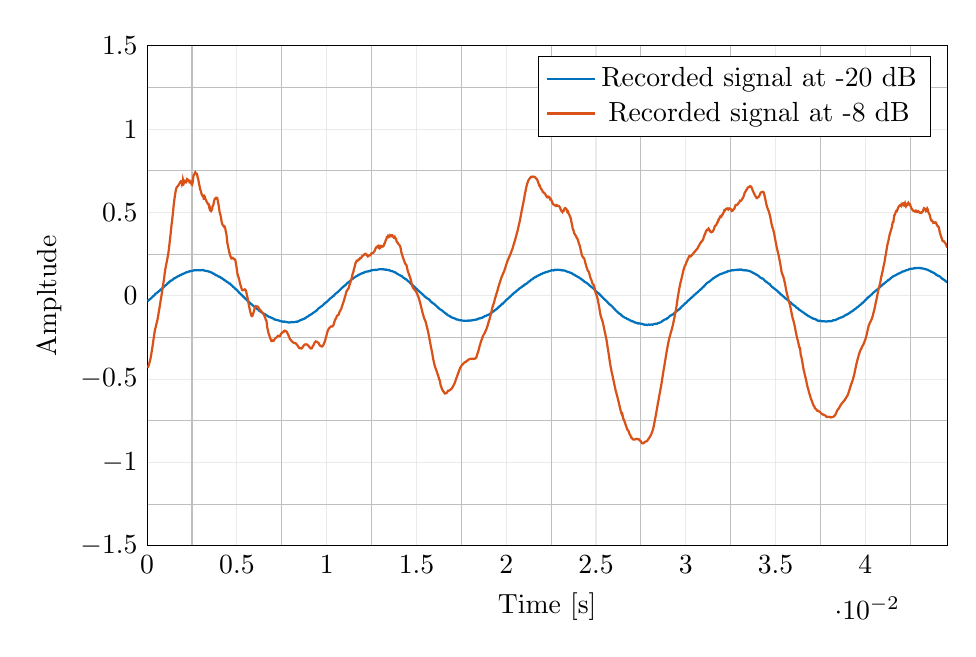
\begin{tikzpicture}

\begin{axis}[%
width=4in,
height=2.5in,
    grid = both,
    minor tick num=1,
    every major grid/.style={opacity=0.3},
    major tick length=0pt,
    minor tick length=0pt,
scale only axis,
xmin=0,
xmax=0.0445578231292517,
xlabel={Time [s]},
ymin=-1.5,
ymax=1.5,
ylabel={Ampltude},
axis background/.style={fill=white}
]
\addplot [color=mycolor1,solid,thick]
  table[row sep=crcr]{%
2.26757369614512e-05	-0.0328369140625\\
4.53514739229025e-05	-0.02972412109375\\
6.80272108843537e-05	-0.027435302734375\\
9.0702947845805e-05	-0.024932861328125\\
0.000113378684807256	-0.023895263671875\\
0.000136054421768707	-0.02191162109375\\
0.000158730158730159	-0.01983642578125\\
0.00018140589569161	-0.018402099609375\\
0.000204081632653061	-0.01605224609375\\
0.000226757369614512	-0.014068603515625\\
0.000249433106575964	-0.011749267578125\\
0.000272108843537415	-0.009124755859375\\
0.000294784580498866	-0.006683349609375\\
0.000317460317460317	-0.00439453125\\
0.000340136054421769	-0.001434326171875\\
0.00036281179138322	0.000579833984375\\
0.000385487528344671	0.001953125\\
0.000408163265306122	0.003631591796875\\
0.000430839002267574	0.007354736328125\\
0.000453514739229025	0.0113525390625\\
0.000476190476190476	0.013397216796875\\
0.000498866213151927	0.01416015625\\
0.000521541950113379	0.0147705078125\\
0.00054421768707483	0.0172119140625\\
0.000566893424036281	0.020050048828125\\
0.000589569160997732	0.021759033203125\\
0.000612244897959184	0.0238037109375\\
0.000634920634920635	0.026397705078125\\
0.000657596371882086	0.027740478515625\\
0.000680272108843537	0.02886962890625\\
0.000702947845804989	0.031829833984375\\
0.00072562358276644	0.03570556640625\\
0.000748299319727891	0.0372314453125\\
0.000770975056689342	0.038848876953125\\
0.000793650793650794	0.041229248046875\\
0.000816326530612245	0.0435791015625\\
0.000839002267573696	0.0457763671875\\
0.000861678004535147	0.047821044921875\\
0.000884353741496599	0.050567626953125\\
0.00090702947845805	0.05145263671875\\
0.000929705215419501	0.052490234375\\
0.000952380952380952	0.0550537109375\\
0.000975056689342404	0.05914306640625\\
0.000997732426303855	0.0614013671875\\
0.00102040816326531	0.062103271484375\\
0.00104308390022676	0.06439208984375\\
0.00106575963718821	0.066558837890625\\
0.00108843537414966	0.068572998046875\\
0.00111111111111111	0.0709228515625\\
0.00113378684807256	0.074066162109375\\
0.00115646258503401	0.076202392578125\\
0.00117913832199546	0.077545166015625\\
0.00120181405895692	0.079559326171875\\
0.00122448979591837	0.0819091796875\\
0.00124716553287982	0.0850830078125\\
0.00126984126984127	0.08746337890625\\
0.00129251700680272	0.08843994140625\\
0.00131519274376417	0.09027099609375\\
0.00133786848072562	0.09173583984375\\
0.00136054421768707	0.0921630859375\\
0.00138321995464853	0.09375\\
0.00140589569160998	0.095672607421875\\
0.00142857142857143	0.097320556640625\\
0.00145124716553288	0.099090576171875\\
0.00147392290249433	0.101531982421875\\
0.00149659863945578	0.104339599609375\\
0.00151927437641723	0.10528564453125\\
0.00154195011337868	0.106475830078125\\
0.00156462585034014	0.107421875\\
0.00158730158730159	0.108673095703125\\
0.00160997732426304	0.1104736328125\\
0.00163265306122449	0.1121826171875\\
0.00165532879818594	0.113677978515625\\
0.00167800453514739	0.11480712890625\\
0.00170068027210884	0.115875244140625\\
0.00172335600907029	0.116790771484375\\
0.00174603174603175	0.118560791015625\\
0.0017687074829932	0.119781494140625\\
0.00179138321995465	0.120635986328125\\
0.0018140589569161	0.122283935546875\\
0.00183673469387755	0.123809814453125\\
0.001859410430839	0.125030517578125\\
0.00188208616780045	0.124969482421875\\
0.0019047619047619	0.1268310546875\\
0.00192743764172336	0.128265380859375\\
0.00195011337868481	0.129302978515625\\
0.00197278911564626	0.130584716796875\\
0.00199546485260771	0.1318359375\\
0.00201814058956916	0.132537841796875\\
0.00204081632653061	0.13311767578125\\
0.00206349206349206	0.134429931640625\\
0.00208616780045351	0.13665771484375\\
0.00210884353741497	0.13739013671875\\
0.00213151927437642	0.137847900390625\\
0.00215419501133787	0.13946533203125\\
0.00217687074829932	0.1407470703125\\
0.00219954648526077	0.14117431640625\\
0.00222222222222222	0.140960693359375\\
0.00224489795918367	0.14215087890625\\
0.00226757369614512	0.143341064453125\\
0.00229024943310658	0.14422607421875\\
0.00231292517006803	0.144805908203125\\
0.00233560090702948	0.146392822265625\\
0.00235827664399093	0.14703369140625\\
0.00238095238095238	0.14642333984375\\
0.00240362811791383	0.14752197265625\\
0.00242630385487528	0.148284912109375\\
0.00244897959183673	0.148406982421875\\
0.00247165532879819	0.149078369140625\\
0.00249433106575964	0.149139404296875\\
0.00251700680272109	0.149993896484375\\
0.00253968253968254	0.151153564453125\\
0.00256235827664399	0.15118408203125\\
0.00258503401360544	0.151702880859375\\
0.00260770975056689	0.153106689453125\\
0.00263038548752834	0.15399169921875\\
0.0026530612244898	0.1534423828125\\
0.00267573696145125	0.1531982421875\\
0.0026984126984127	0.153533935546875\\
0.00272108843537415	0.15338134765625\\
0.0027437641723356	0.153411865234375\\
0.00276643990929705	0.153961181640625\\
0.0027891156462585	0.154144287109375\\
0.00281179138321995	0.15386962890625\\
0.00283446712018141	0.153717041015625\\
0.00285714285714286	0.1539306640625\\
0.00287981859410431	0.153778076171875\\
0.00290249433106576	0.1533203125\\
0.00292517006802721	0.1531982421875\\
0.00294784580498866	0.153472900390625\\
0.00297052154195011	0.153350830078125\\
0.00299319727891156	0.15325927734375\\
0.00301587301587302	0.1533203125\\
0.00303854875283447	0.154144287109375\\
0.00306122448979592	0.15496826171875\\
0.00308390022675737	0.15557861328125\\
0.00310657596371882	0.1551513671875\\
0.00312925170068027	0.153656005859375\\
0.00315192743764172	0.15228271484375\\
0.00317460317460317	0.151397705078125\\
0.00319727891156463	0.151763916015625\\
0.00321995464852608	0.151275634765625\\
0.00324263038548753	0.149658203125\\
0.00326530612244898	0.1494140625\\
0.00328798185941043	0.149505615234375\\
0.00331065759637188	0.149322509765625\\
0.00333333333333333	0.14910888671875\\
0.00335600907029478	0.148101806640625\\
0.00337868480725624	0.14752197265625\\
0.00340136054421769	0.146392822265625\\
0.00342403628117914	0.1461181640625\\
0.00344671201814059	0.145416259765625\\
0.00346938775510204	0.143798828125\\
0.00349206349206349	0.14276123046875\\
0.00351473922902494	0.142303466796875\\
0.00353741496598639	0.1417236328125\\
0.00356009070294785	0.140625\\
0.0035827664399093	0.13922119140625\\
0.00360544217687075	0.1378173828125\\
0.0036281179138322	0.1368408203125\\
0.00365079365079365	0.1356201171875\\
0.0036734693877551	0.133758544921875\\
0.00369614512471655	0.132568359375\\
0.003718820861678	0.132232666015625\\
0.00374149659863946	0.130584716796875\\
0.00376417233560091	0.1282958984375\\
0.00378684807256236	0.12701416015625\\
0.00380952380952381	0.12591552734375\\
0.00383219954648526	0.123687744140625\\
0.00385487528344671	0.1226806640625\\
0.00387755102040816	0.122528076171875\\
0.00390022675736961	0.121734619140625\\
0.00392290249433107	0.118927001953125\\
0.00394557823129252	0.11669921875\\
0.00396825396825397	0.1163330078125\\
0.00399092970521542	0.116241455078125\\
0.00401360544217687	0.1156005859375\\
0.00403628117913832	0.11358642578125\\
0.00405895691609977	0.1124267578125\\
0.00408163265306122	0.1104736328125\\
0.00410430839002268	0.10821533203125\\
0.00412698412698413	0.1068115234375\\
0.00414965986394558	0.106536865234375\\
0.00417233560090703	0.1048583984375\\
0.00419501133786848	0.101898193359375\\
0.00421768707482993	0.100555419921875\\
0.00424036281179138	0.099365234375\\
0.00426303854875283	0.097900390625\\
0.00428571428571429	0.095703125\\
0.00430839002267574	0.094207763671875\\
0.00433106575963719	0.093353271484375\\
0.00435374149659864	0.0906982421875\\
0.00437641723356009	0.08831787109375\\
0.00439909297052154	0.087249755859375\\
0.00442176870748299	0.085906982421875\\
0.00444444444444444	0.084075927734375\\
0.0044671201814059	0.081939697265625\\
0.00448979591836735	0.080902099609375\\
0.0045124716553288	0.079864501953125\\
0.00453514739229025	0.07708740234375\\
0.0045578231292517	0.074920654296875\\
0.00458049886621315	0.073486328125\\
0.0046031746031746	0.073577880859375\\
0.00462585034013605	0.071044921875\\
0.00464852607709751	0.06787109375\\
0.00467120181405896	0.065948486328125\\
0.00469387755102041	0.064178466796875\\
0.00471655328798186	0.06201171875\\
0.00473922902494331	0.0595703125\\
0.00476190476190476	0.057464599609375\\
0.00478458049886621	0.0543212890625\\
0.00480725623582766	0.05194091796875\\
0.00482993197278912	0.050537109375\\
0.00485260770975057	0.049224853515625\\
0.00487528344671202	0.046630859375\\
0.00489795918367347	0.04290771484375\\
0.00492063492063492	0.040374755859375\\
0.00494331065759637	0.03961181640625\\
0.00496598639455782	0.037689208984375\\
0.00498866213151927	0.03509521484375\\
0.00501133786848073	0.033721923828125\\
0.00503401360544218	0.03094482421875\\
0.00505668934240363	0.0269775390625\\
0.00507936507936508	0.024444580078125\\
0.00510204081632653	0.022491455078125\\
0.00512471655328798	0.01904296875\\
0.00514739229024943	0.015899658203125\\
0.00517006802721088	0.014678955078125\\
0.00519274376417234	0.01312255859375\\
0.00521541950113379	0.009857177734375\\
0.00523809523809524	0.007110595703125\\
0.00526077097505669	0.00543212890625\\
0.00528344671201814	0.003265380859375\\
0.00530612244897959	0.00048828125\\
0.00532879818594104	-0.001556396484375\\
0.00535147392290249	-0.00384521484375\\
0.00537414965986395	-0.006439208984375\\
0.0053968253968254	-0.009033203125\\
0.00541950113378685	-0.011688232421875\\
0.0054421768707483	-0.013916015625\\
0.00546485260770975	-0.01617431640625\\
0.0054875283446712	-0.018646240234375\\
0.00551020408163265	-0.021026611328125\\
0.0055328798185941	-0.022247314453125\\
0.00555555555555555	-0.02508544921875\\
0.00557823129251701	-0.0284423828125\\
0.00560090702947846	-0.03082275390625\\
0.00562358276643991	-0.0318603515625\\
0.00564625850340136	-0.033935546875\\
0.00566893424036281	-0.03662109375\\
0.00569160997732426	-0.039215087890625\\
0.00571428571428571	-0.0421142578125\\
0.00573696145124717	-0.043975830078125\\
0.00575963718820862	-0.046478271484375\\
0.00578231292517007	-0.048004150390625\\
0.00580498866213152	-0.04962158203125\\
0.00582766439909297	-0.052490234375\\
0.00585034013605442	-0.05419921875\\
0.00587301587301587	-0.056610107421875\\
0.00589569160997732	-0.059234619140625\\
0.00591836734693878	-0.061187744140625\\
0.00594104308390023	-0.06317138671875\\
0.00596371882086168	-0.064971923828125\\
0.00598639455782313	-0.06671142578125\\
0.00600907029478458	-0.06817626953125\\
0.00603174603174603	-0.069183349609375\\
0.00605442176870748	-0.071868896484375\\
0.00607709750566893	-0.074310302734375\\
0.00609977324263039	-0.07647705078125\\
0.00612244897959184	-0.07861328125\\
0.00614512471655329	-0.080596923828125\\
0.00616780045351474	-0.081634521484375\\
0.00619047619047619	-0.08306884765625\\
0.00621315192743764	-0.08538818359375\\
0.00623582766439909	-0.088958740234375\\
0.00625850340136054	-0.091156005859375\\
0.00628117913832199	-0.0921630859375\\
0.00630385487528345	-0.0936279296875\\
0.0063265306122449	-0.095733642578125\\
0.00634920634920635	-0.0966796875\\
0.0063718820861678	-0.098663330078125\\
0.00639455782312925	-0.100433349609375\\
0.0064172335600907	-0.10113525390625\\
0.00643990929705215	-0.102874755859375\\
0.00646258503401361	-0.10498046875\\
0.00648526077097506	-0.10638427734375\\
0.00650793650793651	-0.107666015625\\
0.00653061224489796	-0.109283447265625\\
0.00655328798185941	-0.110809326171875\\
0.00657596371882086	-0.111907958984375\\
0.00659863945578231	-0.11358642578125\\
0.00662131519274376	-0.115692138671875\\
0.00664399092970522	-0.117156982421875\\
0.00666666666666667	-0.118743896484375\\
0.00668934240362812	-0.119415283203125\\
0.00671201814058957	-0.1209716796875\\
0.00673469387755102	-0.123077392578125\\
0.00675736961451247	-0.1243896484375\\
0.00678004535147392	-0.126068115234375\\
0.00680272108843537	-0.127105712890625\\
0.00682539682539682	-0.127685546875\\
0.00684807256235828	-0.12799072265625\\
0.00687074829931973	-0.128814697265625\\
0.00689342403628118	-0.13043212890625\\
0.00691609977324263	-0.132568359375\\
0.00693877551020408	-0.133453369140625\\
0.00696145124716553	-0.133331298828125\\
0.00698412698412698	-0.13427734375\\
0.00700680272108843	-0.1356201171875\\
0.00702947845804989	-0.137054443359375\\
0.00705215419501134	-0.138763427734375\\
0.00707482993197279	-0.140838623046875\\
0.00709750566893424	-0.14208984375\\
0.00712018140589569	-0.14202880859375\\
0.00714285714285714	-0.142822265625\\
0.00716553287981859	-0.1439208984375\\
0.00718820861678005	-0.1448974609375\\
0.0072108843537415	-0.144805908203125\\
0.00723356009070295	-0.145263671875\\
0.0072562358276644	-0.145721435546875\\
0.00727891156462585	-0.1466064453125\\
0.0073015873015873	-0.147430419921875\\
0.00732426303854875	-0.14752197265625\\
0.0073469387755102	-0.148681640625\\
0.00736961451247166	-0.150543212890625\\
0.00739229024943311	-0.151031494140625\\
0.00741496598639456	-0.151031494140625\\
0.00743764172335601	-0.152435302734375\\
0.00746031746031746	-0.15252685546875\\
0.00748299319727891	-0.15283203125\\
0.00750566893424036	-0.153472900390625\\
0.00752834467120181	-0.154327392578125\\
0.00755102040816326	-0.154876708984375\\
0.00757369614512472	-0.15576171875\\
0.00759637188208617	-0.1556396484375\\
0.00761904761904762	-0.1539306640625\\
0.00764172335600907	-0.153656005859375\\
0.00766439909297052	-0.15484619140625\\
0.00768707482993197	-0.156005859375\\
0.00770975056689342	-0.156768798828125\\
0.00773242630385487	-0.157623291015625\\
0.00775510204081633	-0.15716552734375\\
0.00777777777777778	-0.1573486328125\\
0.00780045351473923	-0.1578369140625\\
0.00782312925170068	-0.15850830078125\\
0.00784580498866213	-0.15899658203125\\
0.00786848072562358	-0.1597900390625\\
0.00789115646258503	-0.16033935546875\\
0.00791383219954649	-0.16058349609375\\
0.00793650793650794	-0.160400390625\\
0.00795918367346939	-0.159149169921875\\
0.00798185941043084	-0.1583251953125\\
0.00800453514739229	-0.15863037109375\\
0.00802721088435374	-0.1585693359375\\
0.00804988662131519	-0.157562255859375\\
0.00807256235827664	-0.157196044921875\\
0.0080952380952381	-0.15771484375\\
0.00811791383219955	-0.15899658203125\\
0.008140589569161	-0.158905029296875\\
0.00816326530612245	-0.158111572265625\\
0.0081859410430839	-0.157684326171875\\
0.00820861678004535	-0.156585693359375\\
0.0082312925170068	-0.15679931640625\\
0.00825396825396825	-0.156280517578125\\
0.00827664399092971	-0.15594482421875\\
0.00829931972789116	-0.155059814453125\\
0.00832199546485261	-0.154815673828125\\
0.00834467120181406	-0.155792236328125\\
0.00836734693877551	-0.155517578125\\
0.00839002267573696	-0.154205322265625\\
0.00841269841269841	-0.15264892578125\\
0.00843537414965987	-0.151611328125\\
0.00845804988662132	-0.1507568359375\\
0.00848072562358277	-0.149505615234375\\
0.00850340136054422	-0.147491455078125\\
0.00852607709750567	-0.146728515625\\
0.00854875283446712	-0.1458740234375\\
0.00857142857142857	-0.14483642578125\\
0.00859410430839002	-0.14447021484375\\
0.00861678004535148	-0.143798828125\\
0.00863945578231293	-0.14178466796875\\
0.00866213151927438	-0.139739990234375\\
0.00868480725623583	-0.139617919921875\\
0.00870748299319728	-0.139923095703125\\
0.00873015873015873	-0.138702392578125\\
0.00875283446712018	-0.1373291015625\\
0.00877551020408163	-0.1361083984375\\
0.00879818594104308	-0.134552001953125\\
0.00882086167800454	-0.13323974609375\\
0.00884353741496599	-0.131500244140625\\
0.00886621315192744	-0.1295166015625\\
0.00888888888888889	-0.126678466796875\\
0.00891156462585034	-0.12518310546875\\
0.00893424036281179	-0.12493896484375\\
0.00895691609977324	-0.123809814453125\\
0.00897959183673469	-0.1221923828125\\
0.00900226757369615	-0.119842529296875\\
0.0090249433106576	-0.11712646484375\\
0.00904761904761905	-0.116302490234375\\
0.0090702947845805	-0.115997314453125\\
0.00909297052154195	-0.114349365234375\\
0.0091156462585034	-0.112060546875\\
0.00913832199546485	-0.110565185546875\\
0.0091609977324263	-0.108978271484375\\
0.00918367346938776	-0.107635498046875\\
0.00920634920634921	-0.10589599609375\\
0.00922902494331066	-0.10406494140625\\
0.00925170068027211	-0.10211181640625\\
0.00927437641723356	-0.100341796875\\
0.00929705215419501	-0.09912109375\\
0.00931972789115646	-0.09722900390625\\
0.00934240362811791	-0.095306396484375\\
0.00936507936507937	-0.094024658203125\\
0.00938775510204082	-0.09228515625\\
0.00941043083900227	-0.090118408203125\\
0.00943310657596372	-0.088226318359375\\
0.00945578231292517	-0.08599853515625\\
0.00947845804988662	-0.0836181640625\\
0.00950113378684807	-0.080535888671875\\
0.00952380952380952	-0.077392578125\\
0.00954648526077098	-0.0758056640625\\
0.00956916099773243	-0.07415771484375\\
0.00959183673469388	-0.0726318359375\\
0.00961451247165533	-0.07061767578125\\
0.00963718820861678	-0.068328857421875\\
0.00965986394557823	-0.0660400390625\\
0.00968253968253968	-0.064208984375\\
0.00970521541950113	-0.06304931640625\\
0.00972789115646258	-0.062164306640625\\
0.00975056689342404	-0.060089111328125\\
0.00977324263038549	-0.058074951171875\\
0.00979591836734694	-0.0557861328125\\
0.00981859410430839	-0.053192138671875\\
0.00984126984126984	-0.050323486328125\\
0.00986394557823129	-0.0474853515625\\
0.00988662131519275	-0.046356201171875\\
0.0099092970521542	-0.044464111328125\\
0.00993197278911565	-0.041748046875\\
0.0099546485260771	-0.039825439453125\\
0.00997732426303855	-0.0382080078125\\
0.01	-0.036590576171875\\
0.0100226757369615	-0.034942626953125\\
0.0100453514739229	-0.032318115234375\\
0.0100680272108844	-0.02935791015625\\
0.0100907029478458	-0.027374267578125\\
0.0101133786848073	-0.025238037109375\\
0.0101360544217687	-0.022552490234375\\
0.0101587301587302	-0.0198974609375\\
0.0101814058956916	-0.016815185546875\\
0.0102040816326531	-0.014434814453125\\
0.0102267573696145	-0.01318359375\\
0.010249433106576	-0.011383056640625\\
0.0102721088435374	-0.0098876953125\\
0.0102947845804989	-0.007965087890625\\
0.0103174603174603	-0.005126953125\\
0.0103401360544218	-0.0029296875\\
0.0103628117913832	-0.00213623046875\\
0.0103854875283447	-0.001007080078125\\
0.0104081632653061	0.00177001953125\\
0.0104308390022676	0.005462646484375\\
0.010453514739229	0.008270263671875\\
0.0104761904761905	0.01031494140625\\
0.0104988662131519	0.012908935546875\\
0.0105215419501134	0.015167236328125\\
0.0105442176870748	0.01617431640625\\
0.0105668934240363	0.018280029296875\\
0.0105895691609977	0.020843505859375\\
0.0106122448979592	0.022064208984375\\
0.0106349206349206	0.02398681640625\\
0.0106575963718821	0.026580810546875\\
0.0106802721088435	0.02972412109375\\
0.010702947845805	0.031494140625\\
0.0107256235827664	0.033843994140625\\
0.0107482993197279	0.036865234375\\
0.0107709750566893	0.0390625\\
0.0107936507936508	0.04156494140625\\
0.0108163265306122	0.04388427734375\\
0.0108390022675737	0.04669189453125\\
0.0108616780045351	0.0487060546875\\
0.0108843537414966	0.050323486328125\\
0.0109070294784581	0.052825927734375\\
0.0109297052154195	0.055419921875\\
0.010952380952381	0.0567626953125\\
0.0109750566893424	0.058563232421875\\
0.0109977324263039	0.061065673828125\\
0.0110204081632653	0.062530517578125\\
0.0110430839002268	0.06451416015625\\
0.0110657596371882	0.06707763671875\\
0.0110884353741497	0.06982421875\\
0.0111111111111111	0.072723388671875\\
0.0111337868480726	0.07489013671875\\
0.011156462585034	0.07708740234375\\
0.0111791383219955	0.079132080078125\\
0.0112018140589569	0.0809326171875\\
0.0112244897959184	0.0823974609375\\
0.0112471655328798	0.08416748046875\\
0.0112698412698413	0.08587646484375\\
0.0112925170068027	0.088043212890625\\
0.0113151927437642	0.089996337890625\\
0.0113378684807256	0.09228515625\\
0.0113605442176871	0.09503173828125\\
0.0113832199546485	0.0972900390625\\
0.01140589569161	0.09942626953125\\
0.0114285714285714	0.100433349609375\\
0.0114512471655329	0.101715087890625\\
0.0114739229024943	0.104583740234375\\
0.0114965986394558	0.10662841796875\\
0.0115192743764172	0.1083984375\\
0.0115419501133787	0.110198974609375\\
0.0115646258503401	0.11138916015625\\
0.0115873015873016	0.112884521484375\\
0.011609977324263	0.11480712890625\\
0.0116326530612245	0.116668701171875\\
0.0116553287981859	0.117950439453125\\
0.0116780045351474	0.1182861328125\\
0.0117006802721088	0.119232177734375\\
0.0117233560090703	0.121429443359375\\
0.0117460317460317	0.123809814453125\\
0.0117687074829932	0.124908447265625\\
0.0117913832199546	0.1265869140625\\
0.0118140589569161	0.127288818359375\\
0.0118367346938776	0.127593994140625\\
0.011859410430839	0.129119873046875\\
0.0118820861678005	0.131317138671875\\
0.0119047619047619	0.132476806640625\\
0.0119274376417234	0.1331787109375\\
0.0119501133786848	0.134002685546875\\
0.0119727891156463	0.135345458984375\\
0.0119954648526077	0.135345458984375\\
0.0120181405895692	0.1363525390625\\
0.0120408163265306	0.138214111328125\\
0.0120634920634921	0.138702392578125\\
0.0120861678004535	0.139923095703125\\
0.012108843537415	0.141754150390625\\
0.0121315192743764	0.14300537109375\\
0.0121541950113379	0.143402099609375\\
0.0121768707482993	0.144195556640625\\
0.0121995464852608	0.145050048828125\\
0.0122222222222222	0.145050048828125\\
0.0122448979591837	0.145599365234375\\
0.0122675736961451	0.146484375\\
0.0122902494331066	0.14593505859375\\
0.012312925170068	0.146270751953125\\
0.0123356009070295	0.14764404296875\\
0.0123582766439909	0.149139404296875\\
0.0123809523809524	0.149444580078125\\
0.0124036281179138	0.14910888671875\\
0.0124263038548753	0.149261474609375\\
0.0124489795918367	0.150970458984375\\
0.0124716553287982	0.152740478515625\\
0.0124943310657596	0.153289794921875\\
0.0125170068027211	0.15325927734375\\
0.0125396825396825	0.1531982421875\\
0.012562358276644	0.154052734375\\
0.0125850340136054	0.154571533203125\\
0.0126077097505669	0.15447998046875\\
0.0126303854875283	0.15460205078125\\
0.0126530612244898	0.1549072265625\\
0.0126757369614512	0.15496826171875\\
0.0126984126984127	0.155975341796875\\
0.0127210884353742	0.155975341796875\\
0.0127437641723356	0.15521240234375\\
0.0127664399092971	0.155029296875\\
0.0127891156462585	0.155853271484375\\
0.01281179138322	0.156158447265625\\
0.0128344671201814	0.1572265625\\
0.0128571428571429	0.157928466796875\\
0.0128798185941043	0.158477783203125\\
0.0129024943310658	0.158660888671875\\
0.0129251700680272	0.158905029296875\\
0.0129478458049887	0.158782958984375\\
0.0129705215419501	0.15899658203125\\
0.0129931972789116	0.15887451171875\\
0.013015873015873	0.158660888671875\\
0.0130385487528345	0.159088134765625\\
0.0130612244897959	0.159271240234375\\
0.0130839002267574	0.159332275390625\\
0.0131065759637188	0.1590576171875\\
0.0131292517006803	0.15960693359375\\
0.0131519274376417	0.16015625\\
0.0131746031746032	0.159393310546875\\
0.0131972789115646	0.157867431640625\\
0.0132199546485261	0.15838623046875\\
0.0132426303854875	0.158477783203125\\
0.013265306122449	0.156585693359375\\
0.0132879818594104	0.155853271484375\\
0.0133106575963719	0.156890869140625\\
0.0133333333333333	0.157440185546875\\
0.0133560090702948	0.156524658203125\\
0.0133786848072562	0.155364990234375\\
0.0134013605442177	0.15557861328125\\
0.0134240362811791	0.154815673828125\\
0.0134467120181406	0.153778076171875\\
0.013469387755102	0.15411376953125\\
0.0134920634920635	0.154815673828125\\
0.0135147392290249	0.152618408203125\\
0.0135374149659864	0.150787353515625\\
0.0135600907029478	0.149505615234375\\
0.0135827664399093	0.148529052734375\\
0.0136054421768707	0.148284912109375\\
0.0136281179138322	0.14788818359375\\
0.0136507936507937	0.14752197265625\\
0.0136734693877551	0.146575927734375\\
0.0136961451247166	0.14599609375\\
0.013718820861678	0.144866943359375\\
0.0137414965986395	0.142913818359375\\
0.0137641723356009	0.1414794921875\\
0.0137868480725624	0.141082763671875\\
0.0138095238095238	0.14105224609375\\
0.0138321995464853	0.139678955078125\\
0.0138548752834467	0.138092041015625\\
0.0138775510204082	0.13580322265625\\
0.0139002267573696	0.13458251953125\\
0.0139229024943311	0.13323974609375\\
0.0139455782312925	0.1309814453125\\
0.013968253968254	0.129638671875\\
0.0139909297052154	0.128204345703125\\
0.0140136054421769	0.127105712890625\\
0.0140362811791383	0.125885009765625\\
0.0140589569160998	0.12457275390625\\
0.0140816326530612	0.123077392578125\\
0.0141043083900227	0.12127685546875\\
0.0141269841269841	0.120208740234375\\
0.0141496598639456	0.119110107421875\\
0.014172335600907	0.1182861328125\\
0.0141950113378685	0.117095947265625\\
0.0142176870748299	0.114959716796875\\
0.0142403628117914	0.11138916015625\\
0.0142630385487528	0.10968017578125\\
0.0142857142857143	0.10858154296875\\
0.0143083900226757	0.107330322265625\\
0.0143310657596372	0.105316162109375\\
0.0143537414965986	0.103057861328125\\
0.0143764172335601	0.100738525390625\\
0.0143990929705215	0.099761962890625\\
0.014421768707483	0.09967041015625\\
0.0144444444444444	0.097747802734375\\
0.0144671201814059	0.094696044921875\\
0.0144897959183673	0.091888427734375\\
0.0145124716553288	0.089996337890625\\
0.0145351473922903	0.08746337890625\\
0.0145578231292517	0.086334228515625\\
0.0145804988662132	0.084869384765625\\
0.0146031746031746	0.083160400390625\\
0.0146258503401361	0.079742431640625\\
0.0146485260770975	0.076171875\\
0.014671201814059	0.0738525390625\\
0.0146938775510204	0.0712890625\\
0.0147165532879819	0.06915283203125\\
0.0147392290249433	0.067779541015625\\
0.0147619047619048	0.06646728515625\\
0.0147845804988662	0.063995361328125\\
0.0148072562358277	0.06103515625\\
0.0148299319727891	0.059326171875\\
0.0148526077097506	0.057525634765625\\
0.014875283446712	0.055328369140625\\
0.0148979591836735	0.052520751953125\\
0.0149206349206349	0.049957275390625\\
0.0149433106575964	0.0472412109375\\
0.0149659863945578	0.04473876953125\\
0.0149886621315193	0.04302978515625\\
0.0150113378684807	0.0411376953125\\
0.0150340136054422	0.038726806640625\\
0.0150566893424036	0.0352783203125\\
0.0150793650793651	0.0333251953125\\
0.0151020408163265	0.031463623046875\\
0.015124716553288	0.028900146484375\\
0.0151473922902494	0.026702880859375\\
0.0151700680272109	0.024627685546875\\
0.0151927437641723	0.022369384765625\\
0.0152154195011338	0.02020263671875\\
0.0152380952380952	0.018829345703125\\
0.0152607709750567	0.016754150390625\\
0.0152834467120181	0.01416015625\\
0.0153061224489796	0.01171875\\
0.015328798185941	0.009429931640625\\
0.0153514739229025	0.007781982421875\\
0.0153741496598639	0.005615234375\\
0.0153968253968254	0.0032958984375\\
0.0154195011337868	0.0009765625\\
0.0154421768707483	-0.00201416015625\\
0.0154648526077098	-0.004364013671875\\
0.0154875283446712	-0.0064697265625\\
0.0155102040816327	-0.00860595703125\\
0.0155328798185941	-0.009735107421875\\
0.0155555555555556	-0.011322021484375\\
0.015578231292517	-0.01348876953125\\
0.0156009070294785	-0.01568603515625\\
0.0156235827664399	-0.01666259765625\\
0.0156462585034014	-0.017852783203125\\
0.0156689342403628	-0.01934814453125\\
0.0156916099773243	-0.021240234375\\
0.0157142857142857	-0.023712158203125\\
0.0157369614512472	-0.026275634765625\\
0.0157596371882086	-0.0291748046875\\
0.0157823129251701	-0.0325927734375\\
0.0158049886621315	-0.035186767578125\\
0.015827664399093	-0.036285400390625\\
0.0158503401360544	-0.038238525390625\\
0.0158730158730159	-0.040802001953125\\
0.0158956916099773	-0.0426025390625\\
0.0159183673469388	-0.044769287109375\\
0.0159410430839002	-0.046173095703125\\
0.0159637188208617	-0.0474853515625\\
0.0159863945578231	-0.048858642578125\\
0.0160090702947846	-0.050628662109375\\
0.016031746031746	-0.05303955078125\\
0.0160544217687075	-0.05584716796875\\
0.0160770975056689	-0.057769775390625\\
0.0160997732426304	-0.06005859375\\
0.0161224489795918	-0.06268310546875\\
0.0161451247165533	-0.065032958984375\\
0.0161678004535147	-0.067047119140625\\
0.0161904761904762	-0.0689697265625\\
0.0162131519274376	-0.0711669921875\\
0.0162358276643991	-0.074493408203125\\
0.0162585034013605	-0.076171875\\
0.016281179138322	-0.07794189453125\\
0.0163038548752834	-0.080352783203125\\
0.0163265306122449	-0.08221435546875\\
0.0163492063492063	-0.082794189453125\\
0.0163718820861678	-0.084136962890625\\
0.0163945578231292	-0.086578369140625\\
0.0164172335600907	-0.087646484375\\
0.0164399092970522	-0.0894775390625\\
0.0164625850340136	-0.091949462890625\\
0.0164852607709751	-0.093994140625\\
0.0165079365079365	-0.0953369140625\\
0.016530612244898	-0.097625732421875\\
0.0165532879818594	-0.100006103515625\\
0.0165759637188209	-0.101837158203125\\
0.0165986394557823	-0.103424072265625\\
0.0166213151927438	-0.105255126953125\\
0.0166439909297052	-0.107421875\\
0.0166666666666667	-0.10906982421875\\
0.0166893424036281	-0.11077880859375\\
0.0167120181405896	-0.11328125\\
0.016734693877551	-0.11529541015625\\
0.0167573696145125	-0.116668701171875\\
0.0167800453514739	-0.117889404296875\\
0.0168027210884354	-0.119140625\\
0.0168253968253968	-0.119598388671875\\
0.0168480725623583	-0.120635986328125\\
0.0168707482993197	-0.123565673828125\\
0.0168934240362812	-0.125885009765625\\
0.0169160997732426	-0.126312255859375\\
0.0169387755102041	-0.127227783203125\\
0.0169614512471655	-0.12939453125\\
0.016984126984127	-0.130645751953125\\
0.0170068027210884	-0.1314697265625\\
0.0170294784580499	-0.132080078125\\
0.0170521541950113	-0.1326904296875\\
0.0170748299319728	-0.133270263671875\\
0.0170975056689342	-0.13458251953125\\
0.0171201814058957	-0.13555908203125\\
0.0171428571428571	-0.135986328125\\
0.0171655328798186	-0.137420654296875\\
0.01718820861678	-0.139556884765625\\
0.0172108843537415	-0.14117431640625\\
0.0172335600907029	-0.14178466796875\\
0.0172562358276644	-0.141876220703125\\
0.0172789115646259	-0.142120361328125\\
0.0173015873015873	-0.14288330078125\\
0.0173242630385488	-0.143218994140625\\
0.0173469387755102	-0.14434814453125\\
0.0173696145124717	-0.145751953125\\
0.0173922902494331	-0.14691162109375\\
0.0174149659863946	-0.147186279296875\\
0.017437641723356	-0.14617919921875\\
0.0174603174603175	-0.146331787109375\\
0.0174829931972789	-0.14691162109375\\
0.0175056689342404	-0.1473388671875\\
0.0175283446712018	-0.1478271484375\\
0.0175510204081633	-0.148406982421875\\
0.0175736961451247	-0.1488037109375\\
0.0175963718820862	-0.1490478515625\\
0.0176190476190476	-0.149383544921875\\
0.0176417233560091	-0.14990234375\\
0.0176643990929705	-0.14990234375\\
0.017687074829932	-0.149688720703125\\
0.0177097505668934	-0.14984130859375\\
0.0177324263038549	-0.149139404296875\\
0.0177551020408163	-0.15008544921875\\
0.0177777777777778	-0.1497802734375\\
0.0178004535147392	-0.149627685546875\\
0.0178231292517007	-0.149749755859375\\
0.0178458049886621	-0.149932861328125\\
0.0178684807256236	-0.149078369140625\\
0.017891156462585	-0.148193359375\\
0.0179138321995465	-0.148590087890625\\
0.0179365079365079	-0.149322509765625\\
0.0179591836734694	-0.1490478515625\\
0.0179818594104308	-0.148284912109375\\
0.0180045351473923	-0.14849853515625\\
0.0180272108843537	-0.148651123046875\\
0.0180498866213152	-0.1480712890625\\
0.0180725623582766	-0.146881103515625\\
0.0180952380952381	-0.147552490234375\\
0.0181179138321995	-0.147216796875\\
0.018140589569161	-0.145751953125\\
0.0181632653061224	-0.144561767578125\\
0.0181859410430839	-0.14483642578125\\
0.0182086167800454	-0.145233154296875\\
0.0182312925170068	-0.144500732421875\\
0.0182539682539683	-0.14404296875\\
0.0182766439909297	-0.144073486328125\\
0.0182993197278912	-0.14361572265625\\
0.0183219954648526	-0.14178466796875\\
0.0183446712018141	-0.14141845703125\\
0.0183673469387755	-0.1422119140625\\
0.018390022675737	-0.1402587890625\\
0.0184126984126984	-0.13824462890625\\
0.0184353741496599	-0.13775634765625\\
0.0184580498866213	-0.1373291015625\\
0.0184807256235828	-0.13616943359375\\
0.0185034013605442	-0.13531494140625\\
0.0185260770975057	-0.13568115234375\\
0.0185487528344671	-0.1353759765625\\
0.0185714285714286	-0.133941650390625\\
0.01859410430839	-0.13287353515625\\
0.0186167800453515	-0.13275146484375\\
0.0186394557823129	-0.132659912109375\\
0.0186621315192744	-0.130157470703125\\
0.0186848072562358	-0.12890625\\
0.0187074829931973	-0.1287841796875\\
0.0187301587301587	-0.12774658203125\\
0.0187528344671202	-0.125762939453125\\
0.0187755102040816	-0.123870849609375\\
0.0187981859410431	-0.122711181640625\\
0.0188208616780045	-0.12152099609375\\
0.018843537414966	-0.12139892578125\\
0.0188662131519274	-0.1207275390625\\
0.0188888888888889	-0.120147705078125\\
0.0189115646258503	-0.118194580078125\\
0.0189342403628118	-0.116729736328125\\
0.0189569160997732	-0.1153564453125\\
0.0189795918367347	-0.11468505859375\\
0.0190022675736961	-0.113922119140625\\
0.0190249433106576	-0.112640380859375\\
0.019047619047619	-0.111572265625\\
0.0190702947845805	-0.110443115234375\\
0.0190929705215419	-0.108673095703125\\
0.0191156462585034	-0.106109619140625\\
0.0191383219954649	-0.104705810546875\\
0.0191609977324263	-0.1031494140625\\
0.0191836734693878	-0.10125732421875\\
0.0192063492063492	-0.09954833984375\\
0.0192290249433107	-0.097503662109375\\
0.0192517006802721	-0.095367431640625\\
0.0192743764172336	-0.09442138671875\\
0.019297052154195	-0.092803955078125\\
0.0193197278911565	-0.091400146484375\\
0.0193424036281179	-0.08941650390625\\
0.0193650793650794	-0.086669921875\\
0.0193877551020408	-0.084747314453125\\
0.0194104308390023	-0.083038330078125\\
0.0194331065759637	-0.081756591796875\\
0.0194557823129252	-0.0799560546875\\
0.0194784580498866	-0.0780029296875\\
0.0195011337868481	-0.07513427734375\\
0.0195238095238095	-0.0731201171875\\
0.019546485260771	-0.071319580078125\\
0.0195691609977324	-0.069000244140625\\
0.0195918367346939	-0.0660400390625\\
0.0196145124716553	-0.06378173828125\\
0.0196371882086168	-0.062530517578125\\
0.0196598639455782	-0.061004638671875\\
0.0196825396825397	-0.058258056640625\\
0.0197052154195011	-0.05517578125\\
0.0197278911564626	-0.053131103515625\\
0.019750566893424	-0.050445556640625\\
0.0197732426303855	-0.04803466796875\\
0.0197959183673469	-0.04766845703125\\
0.0198185941043084	-0.046295166015625\\
0.0198412698412698	-0.04345703125\\
0.0198639455782313	-0.040313720703125\\
0.0198866213151927	-0.037811279296875\\
0.0199092970521542	-0.035552978515625\\
0.0199319727891156	-0.033050537109375\\
0.0199546485260771	-0.030731201171875\\
0.0199773242630385	-0.02783203125\\
0.02	-0.025482177734375\\
0.0200226757369615	-0.023101806640625\\
0.0200453514739229	-0.02105712890625\\
0.0200680272108844	-0.01971435546875\\
0.0200907029478458	-0.017822265625\\
0.0201133786848073	-0.015472412109375\\
0.0201360544217687	-0.012908935546875\\
0.0201587301587302	-0.010498046875\\
0.0201814058956916	-0.008636474609375\\
0.0202040816326531	-0.006072998046875\\
0.0202267573696145	-0.003173828125\\
0.020249433106576	-0.001953125\\
0.0202721088435374	0.0001220703125\\
0.0202947845804989	0.003082275390625\\
0.0203174603174603	0.00628662109375\\
0.0203401360544218	0.007843017578125\\
0.0203628117913832	0.009490966796875\\
0.0203854875283447	0.01275634765625\\
0.0204081632653061	0.014892578125\\
0.0204308390022676	0.016632080078125\\
0.020453514739229	0.018951416015625\\
0.0204761904761905	0.020233154296875\\
0.0204988662131519	0.0220947265625\\
0.0205215419501134	0.024078369140625\\
0.0205442176870748	0.026092529296875\\
0.0205668934240363	0.028778076171875\\
0.0205895691609977	0.0303955078125\\
0.0206122448979592	0.032073974609375\\
0.0206349206349206	0.034942626953125\\
0.0206575963718821	0.037384033203125\\
0.0206802721088435	0.0380859375\\
0.020702947845805	0.03985595703125\\
0.0207256235827664	0.042572021484375\\
0.0207482993197279	0.044830322265625\\
0.0207709750566893	0.04681396484375\\
0.0207936507936508	0.047882080078125\\
0.0208163265306122	0.049774169921875\\
0.0208390022675737	0.0513916015625\\
0.0208616780045351	0.0531005859375\\
0.0208843537414966	0.055084228515625\\
0.020907029478458	0.057342529296875\\
0.0209297052154195	0.05841064453125\\
0.020952380952381	0.05938720703125\\
0.0209750566893424	0.062042236328125\\
0.0209977324263039	0.064697265625\\
0.0210204081632653	0.0672607421875\\
0.0210430839002268	0.06768798828125\\
0.0210657596371882	0.0694580078125\\
0.0210884353741497	0.07049560546875\\
0.0211111111111111	0.07183837890625\\
0.0211337868480726	0.0733642578125\\
0.021156462585034	0.0748291015625\\
0.0211791383219955	0.077484130859375\\
0.0212018140589569	0.079345703125\\
0.0212244897959184	0.08148193359375\\
0.0212471655328798	0.084564208984375\\
0.0212698412698413	0.08587646484375\\
0.0212925170068027	0.0865478515625\\
0.0213151927437642	0.088470458984375\\
0.0213378684807256	0.090667724609375\\
0.0213605442176871	0.09368896484375\\
0.0213832199546485	0.095977783203125\\
0.02140589569161	0.097015380859375\\
0.0214285714285714	0.09808349609375\\
0.0214512471655329	0.100006103515625\\
0.0214739229024943	0.10205078125\\
0.0214965986394558	0.103271484375\\
0.0215192743764172	0.10540771484375\\
0.0215419501133787	0.10809326171875\\
0.0215646258503401	0.109222412109375\\
0.0215873015873016	0.1097412109375\\
0.021609977324263	0.1112060546875\\
0.0216326530612245	0.113494873046875\\
0.0216553287981859	0.114715576171875\\
0.0216780045351474	0.114593505859375\\
0.0217006802721088	0.11676025390625\\
0.0217233560090703	0.11883544921875\\
0.0217460317460317	0.119842529296875\\
0.0217687074829932	0.12091064453125\\
0.0217913832199546	0.1220703125\\
0.0218140589569161	0.124114990234375\\
0.0218367346938775	0.124237060546875\\
0.021859410430839	0.125\\
0.0218820861678005	0.1268310546875\\
0.0219047619047619	0.128692626953125\\
0.0219274376417234	0.130584716796875\\
0.0219501133786848	0.130706787109375\\
0.0219727891156463	0.130859375\\
0.0219954648526077	0.13232421875\\
0.0220181405895692	0.133819580078125\\
0.0220408163265306	0.135009765625\\
0.0220634920634921	0.136627197265625\\
0.0220861678004535	0.137298583984375\\
0.022108843537415	0.137969970703125\\
0.0221315192743764	0.13836669921875\\
0.0221541950113379	0.139373779296875\\
0.0221768707482993	0.141082763671875\\
0.0221995464852608	0.141876220703125\\
0.0222222222222222	0.142181396484375\\
0.0222448979591837	0.1429443359375\\
0.0222675736961451	0.14337158203125\\
0.0222902494331066	0.14337158203125\\
0.022312925170068	0.144500732421875\\
0.0223356009070295	0.146514892578125\\
0.0223582766439909	0.14691162109375\\
0.0223809523809524	0.14788818359375\\
0.0224036281179138	0.1484375\\
0.0224263038548753	0.14935302734375\\
0.0224489795918367	0.15008544921875\\
0.0224716553287982	0.1502685546875\\
0.0224943310657596	0.1510009765625\\
0.0225170068027211	0.15301513671875\\
0.0225396825396825	0.15380859375\\
0.022562358276644	0.153045654296875\\
0.0225850340136054	0.152587890625\\
0.0226077097505669	0.15240478515625\\
0.0226303854875283	0.152252197265625\\
0.0226530612244898	0.1529541015625\\
0.0226757369614512	0.155029296875\\
0.0226984126984127	0.1561279296875\\
0.0227210884353742	0.156005859375\\
0.0227437641723356	0.155181884765625\\
0.0227664399092971	0.1553955078125\\
0.0227891156462585	0.155120849609375\\
0.02281179138322	0.15582275390625\\
0.0228344671201814	0.156829833984375\\
0.0228571428571429	0.1568603515625\\
0.0228798185941043	0.157012939453125\\
0.0229024943310658	0.15631103515625\\
0.0229251700680272	0.1558837890625\\
0.0229478458049887	0.155364990234375\\
0.0229705215419501	0.1551513671875\\
0.0229931972789116	0.155181884765625\\
0.023015873015873	0.15460205078125\\
0.0230385487528345	0.15472412109375\\
0.0230612244897959	0.15447998046875\\
0.0230839002267574	0.152740478515625\\
0.0231065759637188	0.15203857421875\\
0.0231292517006803	0.152313232421875\\
0.0231519274376417	0.153045654296875\\
0.0231746031746032	0.15264892578125\\
0.0231972789115646	0.152252197265625\\
0.0232199546485261	0.1524658203125\\
0.0232426303854875	0.1514892578125\\
0.023265306122449	0.151123046875\\
0.0232879818594104	0.149444580078125\\
0.0233106575963719	0.148406982421875\\
0.0233333333333333	0.14794921875\\
0.0233560090702948	0.14697265625\\
0.0233786848072562	0.1453857421875\\
0.0234013605442177	0.14459228515625\\
0.0234240362811791	0.14410400390625\\
0.0234467120181406	0.14312744140625\\
0.023469387755102	0.1431884765625\\
0.0234920634920635	0.14276123046875\\
0.0235147392290249	0.141693115234375\\
0.0235374149659864	0.14013671875\\
0.0235600907029478	0.138427734375\\
0.0235827664399093	0.137481689453125\\
0.0236054421768707	0.137451171875\\
0.0236281179138322	0.136932373046875\\
0.0236507936507937	0.1351318359375\\
0.0236734693877551	0.133819580078125\\
0.0236961451247166	0.131988525390625\\
0.023718820861678	0.129486083984375\\
0.0237414965986395	0.128143310546875\\
0.0237641723356009	0.12713623046875\\
0.0237868480725624	0.126617431640625\\
0.0238095238095238	0.125213623046875\\
0.0238321995464853	0.123321533203125\\
0.0238548752834467	0.12152099609375\\
0.0238775510204082	0.120574951171875\\
0.0239002267573696	0.11944580078125\\
0.0239229024943311	0.11785888671875\\
0.0239455782312925	0.11602783203125\\
0.023968253968254	0.114013671875\\
0.0239909297052154	0.11273193359375\\
0.0240136054421769	0.111297607421875\\
0.0240362811791383	0.110595703125\\
0.0240589569160998	0.109619140625\\
0.0240816326530612	0.10748291015625\\
0.0241043083900227	0.10540771484375\\
0.0241269841269841	0.10443115234375\\
0.0241496598639456	0.10321044921875\\
0.024172335600907	0.101409912109375\\
0.0241950113378685	0.09893798828125\\
0.0242176870748299	0.096771240234375\\
0.0242403628117914	0.094879150390625\\
0.0242630385487528	0.093780517578125\\
0.0242857142857143	0.09149169921875\\
0.0243083900226757	0.08941650390625\\
0.0243310657596372	0.0880126953125\\
0.0243537414965986	0.085113525390625\\
0.0243764172335601	0.082733154296875\\
0.0243990929705215	0.081451416015625\\
0.024421768707483	0.080810546875\\
0.0244444444444444	0.079742431640625\\
0.0244671201814059	0.07794189453125\\
0.0244897959183673	0.0762939453125\\
0.0245124716553288	0.074249267578125\\
0.0245351473922902	0.072845458984375\\
0.0245578231292517	0.0711669921875\\
0.0245804988662132	0.06890869140625\\
0.0246031746031746	0.06585693359375\\
0.0246258503401361	0.0633544921875\\
0.0246485260770975	0.061187744140625\\
0.024671201814059	0.059326171875\\
0.0246938775510204	0.0579833984375\\
0.0247165532879819	0.05517578125\\
0.0247392290249433	0.053192138671875\\
0.0247619047619048	0.052154541015625\\
0.0247845804988662	0.050201416015625\\
0.0248072562358277	0.0484619140625\\
0.0248299319727891	0.04644775390625\\
0.0248526077097506	0.044158935546875\\
0.024875283446712	0.041778564453125\\
0.0248979591836735	0.03955078125\\
0.0249206349206349	0.03570556640625\\
0.0249433106575964	0.033905029296875\\
0.0249659863945578	0.03155517578125\\
0.0249886621315193	0.02850341796875\\
0.0250113378684807	0.0262451171875\\
0.0250340136054422	0.023590087890625\\
0.0250566893424036	0.02166748046875\\
0.0250793650793651	0.019775390625\\
0.0251020408163265	0.017791748046875\\
0.025124716553288	0.016448974609375\\
0.0251473922902494	0.01483154296875\\
0.0251700680272109	0.01202392578125\\
0.0251927437641723	0.00933837890625\\
0.0252154195011338	0.00677490234375\\
0.0252380952380952	0.004425048828125\\
0.0252607709750567	0.002044677734375\\
0.0252834467120181	-0.000885009765625\\
0.0253061224489796	-0.00341796875\\
0.025328798185941	-0.005340576171875\\
0.0253514739229025	-0.007720947265625\\
0.0253741496598639	-0.010986328125\\
0.0253968253968254	-0.01348876953125\\
0.0254195011337868	-0.0159912109375\\
0.0254421768707483	-0.01806640625\\
0.0254648526077098	-0.020263671875\\
0.0254875283446712	-0.022552490234375\\
0.0255102040816327	-0.02471923828125\\
0.0255328798185941	-0.026947021484375\\
0.0255555555555556	-0.02880859375\\
0.025578231292517	-0.031005859375\\
0.0256009070294785	-0.033477783203125\\
0.0256235827664399	-0.036651611328125\\
0.0256462585034014	-0.03955078125\\
0.0256689342403628	-0.04193115234375\\
0.0256916099773243	-0.044677734375\\
0.0257142857142857	-0.04730224609375\\
0.0257369614512472	-0.049560546875\\
0.0257596371882086	-0.05157470703125\\
0.0257823129251701	-0.0538330078125\\
0.0258049886621315	-0.05535888671875\\
0.025827664399093	-0.056640625\\
0.0258503401360544	-0.05902099609375\\
0.0258730158730159	-0.061614990234375\\
0.0258956916099773	-0.0643310546875\\
0.0259183673469388	-0.06671142578125\\
0.0259410430839002	-0.068572998046875\\
0.0259637188208617	-0.0716552734375\\
0.0259863945578231	-0.074554443359375\\
0.0260090702947846	-0.077911376953125\\
0.026031746031746	-0.079681396484375\\
0.0260544217687075	-0.08148193359375\\
0.0260770975056689	-0.084808349609375\\
0.0260997732426304	-0.087493896484375\\
0.0261224489795918	-0.09002685546875\\
0.0261451247165533	-0.09271240234375\\
0.0261678004535147	-0.094482421875\\
0.0261904761904762	-0.096038818359375\\
0.0262131519274376	-0.0986328125\\
0.0262358276643991	-0.1015625\\
0.0262585034013605	-0.103607177734375\\
0.026281179138322	-0.10504150390625\\
0.0263038548752834	-0.1070556640625\\
0.0263265306122449	-0.108428955078125\\
0.0263492063492063	-0.110107421875\\
0.0263718820861678	-0.111663818359375\\
0.0263945578231293	-0.113739013671875\\
0.0264172335600907	-0.1162109375\\
0.0264399092970522	-0.11865234375\\
0.0264625850340136	-0.121124267578125\\
0.0264852607709751	-0.12310791015625\\
0.0265079365079365	-0.12451171875\\
0.026530612244898	-0.1265869140625\\
0.0265532879818594	-0.127532958984375\\
0.0265759637188209	-0.12890625\\
0.0265986394557823	-0.130340576171875\\
0.0266213151927438	-0.1319580078125\\
0.0266439909297052	-0.133514404296875\\
0.0266666666666667	-0.134002685546875\\
0.0266893424036281	-0.13482666015625\\
0.0267120181405896	-0.136871337890625\\
0.026734693877551	-0.138763427734375\\
0.0267573696145125	-0.1392822265625\\
0.0267800453514739	-0.139617919921875\\
0.0268027210884354	-0.141326904296875\\
0.0268253968253968	-0.14288330078125\\
0.0268480725623583	-0.1435546875\\
0.0268707482993197	-0.14508056640625\\
0.0268934240362812	-0.14691162109375\\
0.0269160997732426	-0.147796630859375\\
0.0269387755102041	-0.149505615234375\\
0.0269614512471655	-0.150634765625\\
0.026984126984127	-0.152099609375\\
0.0270068027210884	-0.1527099609375\\
0.0270294784580499	-0.151824951171875\\
0.0270521541950113	-0.153289794921875\\
0.0270748299319728	-0.15521240234375\\
0.0270975056689342	-0.156646728515625\\
0.0271201814058957	-0.15692138671875\\
0.0271428571428571	-0.157562255859375\\
0.0271655328798186	-0.159759521484375\\
0.02718820861678	-0.160003662109375\\
0.0272108843537415	-0.160308837890625\\
0.0272335600907029	-0.162200927734375\\
0.0272562358276644	-0.16357421875\\
0.0272789115646258	-0.163818359375\\
0.0273015873015873	-0.164093017578125\\
0.0273242630385488	-0.16522216796875\\
0.0273469387755102	-0.166290283203125\\
0.0273696145124717	-0.1656494140625\\
0.0273922902494331	-0.164947509765625\\
0.0274149659863946	-0.165771484375\\
0.027437641723356	-0.166656494140625\\
0.0274603174603175	-0.16668701171875\\
0.0274829931972789	-0.16729736328125\\
0.0275056689342404	-0.168212890625\\
0.0275283446712018	-0.16796875\\
0.0275510204081633	-0.16802978515625\\
0.0275736961451247	-0.1685791015625\\
0.0275963718820862	-0.170379638671875\\
0.0276190476190476	-0.17034912109375\\
0.0276417233560091	-0.170684814453125\\
0.0276643990929705	-0.17193603515625\\
0.027687074829932	-0.172698974609375\\
0.0277097505668934	-0.1739501953125\\
0.0277324263038549	-0.17327880859375\\
0.0277551020408163	-0.17340087890625\\
0.0277777777777778	-0.173828125\\
0.0278004535147392	-0.17401123046875\\
0.0278231292517007	-0.17425537109375\\
0.0278458049886621	-0.1749267578125\\
0.0278684807256236	-0.1746826171875\\
0.027891156462585	-0.17376708984375\\
0.0279138321995465	-0.172607421875\\
0.0279365079365079	-0.17205810546875\\
0.0279591836734694	-0.172698974609375\\
0.0279818594104308	-0.173614501953125\\
0.0280045351473923	-0.17425537109375\\
0.0280272108843537	-0.173736572265625\\
0.0280498866213152	-0.172698974609375\\
0.0280725623582766	-0.172821044921875\\
0.0280952380952381	-0.172760009765625\\
0.0281179138321995	-0.173126220703125\\
0.028140589569161	-0.173614501953125\\
0.0281632653061224	-0.17291259765625\\
0.0281859410430839	-0.171722412109375\\
0.0282086167800454	-0.170074462890625\\
0.0282312925170068	-0.169158935546875\\
0.0282539682539683	-0.168853759765625\\
0.0282766439909297	-0.16925048828125\\
0.0282993197278912	-0.16790771484375\\
0.0283219954648526	-0.167999267578125\\
0.0283446712018141	-0.168609619140625\\
0.0283673469387755	-0.1683349609375\\
0.028390022675737	-0.167938232421875\\
0.0284126984126984	-0.16571044921875\\
0.0284353741496599	-0.164398193359375\\
0.0284580498866213	-0.163818359375\\
0.0284807256235828	-0.163299560546875\\
0.0285034013605442	-0.162322998046875\\
0.0285260770975057	-0.162078857421875\\
0.0285487528344671	-0.1610107421875\\
0.0285714285714286	-0.15960693359375\\
0.02859410430839	-0.159454345703125\\
0.0286167800453515	-0.15802001953125\\
0.0286394557823129	-0.15631103515625\\
0.0286621315192744	-0.15423583984375\\
0.0286848072562358	-0.1519775390625\\
0.0287074829931973	-0.150543212890625\\
0.0287301587301587	-0.14892578125\\
0.0287528344671202	-0.147216796875\\
0.0287755102040816	-0.145782470703125\\
0.0287981859410431	-0.144073486328125\\
0.0288208616780045	-0.143096923828125\\
0.028843537414966	-0.1419677734375\\
0.0288662131519274	-0.141204833984375\\
0.0288888888888889	-0.141357421875\\
0.0289115646258503	-0.1405029296875\\
0.0289342403628118	-0.1383056640625\\
0.0289569160997732	-0.135345458984375\\
0.0289795918367347	-0.13323974609375\\
0.0290022675736961	-0.132232666015625\\
0.0290249433106576	-0.13079833984375\\
0.029047619047619	-0.128631591796875\\
0.0290702947845805	-0.125701904296875\\
0.0290929705215419	-0.123382568359375\\
0.0291156462585034	-0.120941162109375\\
0.0291383219954649	-0.11920166015625\\
0.0291609977324263	-0.11883544921875\\
0.0291836734693878	-0.11761474609375\\
0.0292063492063492	-0.11639404296875\\
0.0292290249433107	-0.11376953125\\
0.0292517006802721	-0.11212158203125\\
0.0292743764172336	-0.1119384765625\\
0.029297052154195	-0.11126708984375\\
0.0293197278911565	-0.1094970703125\\
0.0293424036281179	-0.10650634765625\\
0.0293650793650794	-0.10345458984375\\
0.0293877551020408	-0.10198974609375\\
0.0294104308390023	-0.0997314453125\\
0.0294331065759637	-0.097412109375\\
0.0294557823129252	-0.095367431640625\\
0.0294784580498866	-0.09259033203125\\
0.0295011337868481	-0.090667724609375\\
0.0295238095238095	-0.08905029296875\\
0.029546485260771	-0.0880126953125\\
0.0295691609977324	-0.086273193359375\\
0.0295918367346939	-0.084259033203125\\
0.0296145124716553	-0.08233642578125\\
0.0296371882086168	-0.08074951171875\\
0.0296598639455782	-0.078369140625\\
0.0296825396825397	-0.075408935546875\\
0.0297052154195011	-0.073333740234375\\
0.0297278911564626	-0.071136474609375\\
0.029750566893424	-0.0679931640625\\
0.0297732426303855	-0.0645751953125\\
0.0297959183673469	-0.062530517578125\\
0.0298185941043084	-0.06097412109375\\
0.0298412698412698	-0.05914306640625\\
0.0298639455782313	-0.056488037109375\\
0.0298866213151927	-0.054412841796875\\
0.0299092970521542	-0.051849365234375\\
0.0299319727891156	-0.04864501953125\\
0.0299546485260771	-0.04595947265625\\
0.0299773242630385	-0.044891357421875\\
0.03	-0.043548583984375\\
0.0300226757369614	-0.041656494140625\\
0.0300453514739229	-0.03912353515625\\
0.0300680272108844	-0.036102294921875\\
0.0300907029478458	-0.03302001953125\\
0.0301133786848073	-0.0301513671875\\
0.0301360544217687	-0.02777099609375\\
0.0301587301587302	-0.026580810546875\\
0.0301814058956916	-0.02545166015625\\
0.0302040816326531	-0.022369384765625\\
0.0302267573696145	-0.019317626953125\\
0.030249433106576	-0.0174560546875\\
0.0302721088435374	-0.015472412109375\\
0.0302947845804989	-0.01251220703125\\
0.0303174603174603	-0.010345458984375\\
0.0303401360544218	-0.00933837890625\\
0.0303628117913832	-0.007568359375\\
0.0303854875283447	-0.00506591796875\\
0.0304081632653061	-0.002532958984375\\
0.0304308390022676	0.00030517578125\\
0.030453514739229	0.00299072265625\\
0.0304761904761905	0.005767822265625\\
0.0304988662131519	0.007049560546875\\
0.0305215419501134	0.008392333984375\\
0.0305442176870748	0.010467529296875\\
0.0305668934240363	0.01336669921875\\
0.0305895691609977	0.015838623046875\\
0.0306122448979592	0.01788330078125\\
0.0306349206349206	0.01934814453125\\
0.0306575963718821	0.021240234375\\
0.0306802721088435	0.02325439453125\\
0.030702947845805	0.02581787109375\\
0.0307256235827664	0.028717041015625\\
0.0307482993197279	0.031005859375\\
0.0307709750566893	0.032806396484375\\
0.0307936507936508	0.034637451171875\\
0.0308163265306122	0.03765869140625\\
0.0308390022675737	0.0390625\\
0.0308616780045351	0.041473388671875\\
0.0308843537414966	0.04339599609375\\
0.0309070294784581	0.0462646484375\\
0.0309297052154195	0.049163818359375\\
0.030952380952381	0.050933837890625\\
0.0309750566893424	0.053131103515625\\
0.0309977324263039	0.055419921875\\
0.0310204081632653	0.057647705078125\\
0.0310430839002268	0.06048583984375\\
0.0310657596371882	0.063507080078125\\
0.0310884353741497	0.066070556640625\\
0.0311111111111111	0.068939208984375\\
0.0311337868480726	0.0721435546875\\
0.031156462585034	0.07470703125\\
0.0311791383219955	0.07611083984375\\
0.0312018140589569	0.07757568359375\\
0.0312244897959184	0.079315185546875\\
0.0312471655328798	0.081146240234375\\
0.0312698412698413	0.08294677734375\\
0.0312925170068027	0.084564208984375\\
0.0313151927437642	0.085296630859375\\
0.0313378684807256	0.08685302734375\\
0.0313605442176871	0.0892333984375\\
0.0313832199546485	0.09222412109375\\
0.03140589569161	0.093780517578125\\
0.0314285714285714	0.09552001953125\\
0.0314512471655329	0.098052978515625\\
0.0314739229024943	0.099456787109375\\
0.0314965986394558	0.101165771484375\\
0.0315192743764172	0.104217529296875\\
0.0315419501133787	0.105865478515625\\
0.0315646258503401	0.10687255859375\\
0.0315873015873016	0.10833740234375\\
0.031609977324263	0.110321044921875\\
0.0316326530612245	0.112060546875\\
0.0316553287981859	0.11334228515625\\
0.0316780045351474	0.115234375\\
0.0317006802721088	0.116851806640625\\
0.0317233560090703	0.117095947265625\\
0.0317460317460317	0.118255615234375\\
0.0317687074829932	0.12060546875\\
0.0317913832199547	0.122039794921875\\
0.0318140589569161	0.12371826171875\\
0.0318367346938776	0.124908447265625\\
0.031859410430839	0.1263427734375\\
0.0318820861678005	0.127777099609375\\
0.0319047619047619	0.12884521484375\\
0.0319274376417234	0.129974365234375\\
0.0319501133786848	0.131195068359375\\
0.0319727891156463	0.1322021484375\\
0.0319954648526077	0.132568359375\\
0.0320181405895692	0.132965087890625\\
0.0320408163265306	0.1336669921875\\
0.0320634920634921	0.135101318359375\\
0.0320861678004535	0.136260986328125\\
0.032108843537415	0.137176513671875\\
0.0321315192743764	0.137725830078125\\
0.0321541950113379	0.13946533203125\\
0.0321768707482993	0.1396484375\\
0.0321995464852608	0.140045166015625\\
0.0322222222222222	0.140899658203125\\
0.0322448979591837	0.14202880859375\\
0.0322675736961451	0.1431884765625\\
0.0322902494331066	0.143798828125\\
0.032312925170068	0.146026611328125\\
0.0323356009070295	0.147735595703125\\
0.0323582766439909	0.14752197265625\\
0.0323809523809524	0.147857666015625\\
0.0324036281179138	0.14910888671875\\
0.0324263038548753	0.149261474609375\\
0.0324489795918367	0.149322509765625\\
0.0324716553287982	0.150238037109375\\
0.0324943310657596	0.151123046875\\
0.0325170068027211	0.151763916015625\\
0.0325396825396825	0.152191162109375\\
0.032562358276644	0.1534423828125\\
0.0325850340136054	0.153717041015625\\
0.0326077097505669	0.153289794921875\\
0.0326303854875283	0.152557373046875\\
0.0326530612244898	0.15289306640625\\
0.0326757369614512	0.154022216796875\\
0.0326984126984127	0.15423583984375\\
0.0327210884353741	0.154998779296875\\
0.0327437641723356	0.155517578125\\
0.032766439909297	0.15521240234375\\
0.0327891156462585	0.154998779296875\\
0.03281179138322	0.1556396484375\\
0.0328344671201814	0.156494140625\\
0.0328571428571429	0.155853271484375\\
0.0328798185941043	0.15533447265625\\
0.0329024943310658	0.155853271484375\\
0.0329251700680272	0.15625\\
0.0329478458049887	0.15643310546875\\
0.0329705215419501	0.157867431640625\\
0.0329931972789116	0.158111572265625\\
0.033015873015873	0.156951904296875\\
0.0330385487528345	0.155975341796875\\
0.0330612244897959	0.1561279296875\\
0.0330839002267574	0.157073974609375\\
0.0331065759637188	0.15753173828125\\
0.0331292517006803	0.156494140625\\
0.0331519274376417	0.155059814453125\\
0.0331746031746032	0.154541015625\\
0.0331972789115646	0.153411865234375\\
0.0332199546485261	0.152801513671875\\
0.0332426303854875	0.15362548828125\\
0.033265306122449	0.153045654296875\\
0.0332879818594104	0.1522216796875\\
0.0333106575963719	0.152984619140625\\
0.0333333333333333	0.153839111328125\\
0.0333560090702948	0.1529541015625\\
0.0333786848072562	0.152099609375\\
0.0334013605442177	0.151885986328125\\
0.0334240362811791	0.151763916015625\\
0.0334467120181406	0.15142822265625\\
0.033469387755102	0.15032958984375\\
0.0334920634920635	0.150054931640625\\
0.0335147392290249	0.149078369140625\\
0.0335374149659864	0.14825439453125\\
0.0335600907029478	0.148345947265625\\
0.0335827664399093	0.14764404296875\\
0.0336054421768707	0.146331787109375\\
0.0336281179138322	0.144927978515625\\
0.0336507936507937	0.14306640625\\
0.0336734693877551	0.142120361328125\\
0.0336961451247166	0.141204833984375\\
0.033718820861678	0.13922119140625\\
0.0337414965986395	0.13818359375\\
0.0337641723356009	0.137664794921875\\
0.0337868480725624	0.136016845703125\\
0.0338095238095238	0.134521484375\\
0.0338321995464853	0.133514404296875\\
0.0338548752834467	0.1322021484375\\
0.0338775510204082	0.130767822265625\\
0.0339002267573696	0.12921142578125\\
0.0339229024943311	0.127655029296875\\
0.0339455782312925	0.126068115234375\\
0.033968253968254	0.1251220703125\\
0.0339909297052154	0.123382568359375\\
0.0340136054421769	0.1217041015625\\
0.0340362811791383	0.120574951171875\\
0.0340589569160998	0.11871337890625\\
0.0340816326530612	0.116302490234375\\
0.0341043083900227	0.113555908203125\\
0.0341269841269841	0.111328125\\
0.0341496598639456	0.110260009765625\\
0.034172335600907	0.10888671875\\
0.0341950113378685	0.107025146484375\\
0.0342176870748299	0.1053466796875\\
0.0342403628117914	0.10394287109375\\
0.0342630385487528	0.103790283203125\\
0.0342857142857143	0.10321044921875\\
0.0343083900226757	0.10235595703125\\
0.0343310657596372	0.09930419921875\\
0.0343537414965986	0.096038818359375\\
0.0343764172335601	0.093414306640625\\
0.0343990929705215	0.090850830078125\\
0.034421768707483	0.08917236328125\\
0.0344444444444444	0.086761474609375\\
0.0344671201814059	0.08453369140625\\
0.0344897959183673	0.082855224609375\\
0.0345124716553288	0.081451416015625\\
0.0345351473922903	0.080078125\\
0.0345578231292517	0.078399658203125\\
0.0345804988662132	0.07611083984375\\
0.0346031746031746	0.073974609375\\
0.0346258503401361	0.07257080078125\\
0.0346485260770975	0.072052001953125\\
0.034671201814059	0.0703125\\
0.0346938775510204	0.067840576171875\\
0.0347165532879819	0.06365966796875\\
0.0347392290249433	0.06024169921875\\
0.0347619047619048	0.057861328125\\
0.0347845804988662	0.05517578125\\
0.0348072562358277	0.053619384765625\\
0.0348299319727891	0.0521240234375\\
0.0348526077097506	0.04998779296875\\
0.034875283446712	0.047637939453125\\
0.0348979591836735	0.0457763671875\\
0.0349206349206349	0.044097900390625\\
0.0349433106575964	0.0423583984375\\
0.0349659863945578	0.040435791015625\\
0.0349886621315193	0.03863525390625\\
0.0350113378684807	0.036773681640625\\
0.0350340136054422	0.03460693359375\\
0.0350566893424036	0.03277587890625\\
0.0350793650793651	0.031219482421875\\
0.0351020408163265	0.029144287109375\\
0.035124716553288	0.026214599609375\\
0.0351473922902494	0.0230712890625\\
0.0351700680272109	0.0203857421875\\
0.0351927437641723	0.019500732421875\\
0.0352154195011338	0.0177001953125\\
0.0352380952380952	0.01513671875\\
0.0352607709750567	0.0125732421875\\
0.0352834467120181	0.00921630859375\\
0.0353061224489796	0.007476806640625\\
0.035328798185941	0.00604248046875\\
0.0353514739229025	0.00445556640625\\
0.0353741496598639	0.00238037109375\\
0.0353968253968254	-0.0006103515625\\
0.0354195011337868	-0.002655029296875\\
0.0354421768707483	-0.0045166015625\\
0.0354648526077097	-0.0059814453125\\
0.0354875283446712	-0.008575439453125\\
0.0355102040816327	-0.011962890625\\
0.0355328798185941	-0.014556884765625\\
0.0355555555555556	-0.015533447265625\\
0.035578231292517	-0.0166015625\\
0.0356009070294785	-0.01904296875\\
0.0356235827664399	-0.020843505859375\\
0.0356462585034014	-0.02313232421875\\
0.0356689342403628	-0.0247802734375\\
0.0356916099773243	-0.02593994140625\\
0.0357142857142857	-0.02679443359375\\
0.0357369614512472	-0.02960205078125\\
0.0357596371882086	-0.0330810546875\\
0.0357823129251701	-0.03564453125\\
0.0358049886621315	-0.03778076171875\\
0.035827664399093	-0.0386962890625\\
0.0358503401360544	-0.040802001953125\\
0.0358730158730159	-0.043670654296875\\
0.0358956916099773	-0.045989990234375\\
0.0359183673469388	-0.04827880859375\\
0.0359410430839002	-0.049896240234375\\
0.0359637188208617	-0.052581787109375\\
0.0359863945578231	-0.054412841796875\\
0.0360090702947846	-0.05560302734375\\
0.036031746031746	-0.058013916015625\\
0.0360544217687075	-0.0594482421875\\
0.0360770975056689	-0.06048583984375\\
0.0360997732426304	-0.0621337890625\\
0.0361224489795918	-0.065460205078125\\
0.0361451247165533	-0.069061279296875\\
0.0361678004535147	-0.070709228515625\\
0.0361904761904762	-0.07171630859375\\
0.0362131519274376	-0.072998046875\\
0.0362358276643991	-0.0743408203125\\
0.0362585034013605	-0.07696533203125\\
0.036281179138322	-0.079803466796875\\
0.0363038548752834	-0.082275390625\\
0.0363265306122449	-0.084259033203125\\
0.0363492063492063	-0.08563232421875\\
0.0363718820861678	-0.0865478515625\\
0.0363945578231293	-0.087982177734375\\
0.0364172335600907	-0.09027099609375\\
0.0364399092970522	-0.092926025390625\\
0.0364625850340136	-0.09429931640625\\
0.0364852607709751	-0.09564208984375\\
0.0365079365079365	-0.097625732421875\\
0.036530612244898	-0.09918212890625\\
0.0365532879818594	-0.099884033203125\\
0.0365759637188209	-0.101593017578125\\
0.0365986394557823	-0.10394287109375\\
0.0366213151927438	-0.105987548828125\\
0.0366439909297052	-0.10784912109375\\
0.0366666666666667	-0.108795166015625\\
0.0366893424036281	-0.1109619140625\\
0.0367120181405896	-0.112823486328125\\
0.036734693877551	-0.113616943359375\\
0.0367573696145125	-0.11529541015625\\
0.0367800453514739	-0.11810302734375\\
0.0368027210884354	-0.119720458984375\\
0.0368253968253968	-0.120697021484375\\
0.0368480725623583	-0.122406005859375\\
0.0368707482993197	-0.123870849609375\\
0.0368934240362812	-0.12445068359375\\
0.0369160997732426	-0.125946044921875\\
0.0369387755102041	-0.128326416015625\\
0.0369614512471655	-0.12945556640625\\
0.036984126984127	-0.13055419921875\\
0.0370068027210884	-0.131744384765625\\
0.0370294784580499	-0.1326904296875\\
0.0370521541950113	-0.133148193359375\\
0.0370748299319728	-0.1353759765625\\
0.0370975056689342	-0.1373291015625\\
0.0371201814058957	-0.137359619140625\\
0.0371428571428571	-0.13726806640625\\
0.0371655328798186	-0.138641357421875\\
0.03718820861678	-0.139190673828125\\
0.0372108843537415	-0.139190673828125\\
0.0372335600907029	-0.140533447265625\\
0.0372562358276644	-0.14276123046875\\
0.0372789115646259	-0.144805908203125\\
0.0373015873015873	-0.14532470703125\\
0.0373242630385488	-0.1470947265625\\
0.0373469387755102	-0.14892578125\\
0.0373696145124717	-0.15008544921875\\
0.0373922902494331	-0.149658203125\\
0.0374149659863946	-0.149200439453125\\
0.037437641723356	-0.15057373046875\\
0.0374603174603175	-0.150604248046875\\
0.0374829931972789	-0.15020751953125\\
0.0375056689342404	-0.150146484375\\
0.0375283446712018	-0.151519775390625\\
0.0375510204081633	-0.152191162109375\\
0.0375736961451247	-0.152252197265625\\
0.0375963718820862	-0.152618408203125\\
0.0376190476190476	-0.15313720703125\\
0.0376417233560091	-0.152923583984375\\
0.0376643990929705	-0.152099609375\\
0.037687074829932	-0.15216064453125\\
0.0377097505668934	-0.15289306640625\\
0.0377324263038549	-0.152923583984375\\
0.0377551020408163	-0.153533935546875\\
0.0377777777777778	-0.154266357421875\\
0.0378004535147392	-0.1546630859375\\
0.0378231292517007	-0.15484619140625\\
0.0378458049886621	-0.15411376953125\\
0.0378684807256236	-0.15362548828125\\
0.037891156462585	-0.153045654296875\\
0.0379138321995465	-0.15325927734375\\
0.0379365079365079	-0.153076171875\\
0.0379591836734694	-0.15234375\\
0.0379818594104308	-0.152557373046875\\
0.0380045351473923	-0.15252685546875\\
0.0380272108843537	-0.151702880859375\\
0.0380498866213152	-0.152130126953125\\
0.0380725623582766	-0.152984619140625\\
0.0380952380952381	-0.15283203125\\
0.0381179138321995	-0.1512451171875\\
0.038140589569161	-0.150787353515625\\
0.0381632653061224	-0.14935302734375\\
0.0381859410430839	-0.14715576171875\\
0.0382086167800453	-0.146240234375\\
0.0382312925170068	-0.146209716796875\\
0.0382539682539683	-0.14642333984375\\
0.0382766439909297	-0.14691162109375\\
0.0382993197278912	-0.146240234375\\
0.0383219954648526	-0.145263671875\\
0.0383446712018141	-0.14447021484375\\
0.0383673469387755	-0.14300537109375\\
0.038390022675737	-0.141754150390625\\
0.0384126984126984	-0.1407470703125\\
0.0384353741496599	-0.139923095703125\\
0.0384580498866213	-0.13873291015625\\
0.0384807256235828	-0.1380615234375\\
0.0385034013605442	-0.13641357421875\\
0.0385260770975057	-0.134429931640625\\
0.0385487528344671	-0.133636474609375\\
0.0385714285714286	-0.13323974609375\\
0.03859410430839	-0.132110595703125\\
0.0386167800453515	-0.130950927734375\\
0.0386394557823129	-0.13031005859375\\
0.0386621315192744	-0.130157470703125\\
0.0386848072562358	-0.129058837890625\\
0.0387074829931973	-0.12725830078125\\
0.0387301587301587	-0.126373291015625\\
0.0387528344671202	-0.1258544921875\\
0.0387755102040816	-0.12445068359375\\
0.0387981859410431	-0.122955322265625\\
0.0388208616780045	-0.121978759765625\\
0.038843537414966	-0.119873046875\\
0.0388662131519274	-0.11798095703125\\
0.0388888888888889	-0.1160888671875\\
0.0389115646258503	-0.114776611328125\\
0.0389342403628118	-0.114227294921875\\
0.0389569160997732	-0.1136474609375\\
0.0389795918367347	-0.111602783203125\\
0.0390022675736961	-0.110595703125\\
0.0390249433106576	-0.10980224609375\\
0.039047619047619	-0.107635498046875\\
0.0390702947845805	-0.105743408203125\\
0.0390929705215419	-0.104461669921875\\
0.0391156462585034	-0.103179931640625\\
0.0391383219954649	-0.101654052734375\\
0.0391609977324263	-0.0994873046875\\
0.0391836734693878	-0.097503662109375\\
0.0392063492063492	-0.09552001953125\\
0.0392290249433107	-0.094146728515625\\
0.0392517006802721	-0.09356689453125\\
0.0392743764172336	-0.092041015625\\
0.039297052154195	-0.090240478515625\\
0.0393197278911565	-0.08880615234375\\
0.0393424036281179	-0.086334228515625\\
0.0393650793650794	-0.083648681640625\\
0.0393877551020408	-0.08221435546875\\
0.0394104308390023	-0.08111572265625\\
0.0394331065759637	-0.07916259765625\\
0.0394557823129252	-0.07769775390625\\
0.0394784580498866	-0.07586669921875\\
0.0395011337868481	-0.072784423828125\\
0.0395238095238095	-0.07049560546875\\
0.039546485260771	-0.06927490234375\\
0.0395691609977324	-0.06781005859375\\
0.0395918367346939	-0.066619873046875\\
0.0396145124716553	-0.06475830078125\\
0.0396371882086168	-0.061279296875\\
0.0396598639455782	-0.05914306640625\\
0.0396825396825397	-0.057586669921875\\
0.0397052154195011	-0.0552978515625\\
0.0397278911564626	-0.053558349609375\\
0.039750566893424	-0.051788330078125\\
0.0397732426303855	-0.049774169921875\\
0.0397959183673469	-0.0465087890625\\
0.0398185941043084	-0.043914794921875\\
0.0398412698412698	-0.042388916015625\\
0.0398639455782313	-0.041473388671875\\
0.0398866213151927	-0.039093017578125\\
0.0399092970521542	-0.0367431640625\\
0.0399319727891156	-0.034027099609375\\
0.0399546485260771	-0.0313720703125\\
0.0399773242630386	-0.028228759765625\\
0.04	-0.02587890625\\
0.0400226757369615	-0.02447509765625\\
0.0400453514739229	-0.0216064453125\\
0.0400680272108844	-0.018646240234375\\
0.0400907029478458	-0.015380859375\\
0.0401133786848073	-0.01416015625\\
0.0401360544217687	-0.011688232421875\\
0.0401587301587302	-0.00823974609375\\
0.0401814058956916	-0.00653076171875\\
0.0402040816326531	-0.006195068359375\\
0.0402267573696145	-0.004241943359375\\
0.040249433106576	-0.00079345703125\\
0.0402721088435374	0.0008544921875\\
0.0402947845804989	0.002716064453125\\
0.0403174603174603	0.005645751953125\\
0.0403401360544218	0.006988525390625\\
0.0403628117913832	0.0084228515625\\
0.0403854875283447	0.011688232421875\\
0.0404081632653061	0.015350341796875\\
0.0404308390022676	0.017608642578125\\
0.040453514739229	0.01873779296875\\
0.0404761904761905	0.0216064453125\\
0.0404988662131519	0.02362060546875\\
0.0405215419501134	0.025360107421875\\
0.0405442176870748	0.0274658203125\\
0.0405668934240363	0.029876708984375\\
0.0405895691609977	0.032379150390625\\
0.0406122448979592	0.033477783203125\\
0.0406349206349206	0.035369873046875\\
0.0406575963718821	0.037384033203125\\
0.0406802721088435	0.039154052734375\\
0.040702947845805	0.040618896484375\\
0.0407256235827664	0.04290771484375\\
0.0407482993197279	0.04541015625\\
0.0407709750566893	0.04705810546875\\
0.0407936507936508	0.049530029296875\\
0.0408163265306122	0.052215576171875\\
0.0408390022675737	0.0555419921875\\
0.0408616780045351	0.057861328125\\
0.0408843537414966	0.058990478515625\\
0.040907029478458	0.06024169921875\\
0.0409297052154195	0.062530517578125\\
0.040952380952381	0.06591796875\\
0.0409750566893424	0.06854248046875\\
0.0409977324263039	0.070281982421875\\
0.0410204081632653	0.071533203125\\
0.0410430839002268	0.073150634765625\\
0.0410657596371882	0.074798583984375\\
0.0410884353741497	0.07672119140625\\
0.0411111111111111	0.079559326171875\\
0.0411337868480726	0.081634521484375\\
0.041156462585034	0.082855224609375\\
0.0411791383219955	0.0853271484375\\
0.0412018140589569	0.0877685546875\\
0.0412244897959184	0.089599609375\\
0.0412471655328798	0.09173583984375\\
0.0412698412698413	0.09423828125\\
0.0412925170068027	0.09527587890625\\
0.0413151927437642	0.09539794921875\\
0.0413378684807256	0.097747802734375\\
0.0413605442176871	0.100799560546875\\
0.0413832199546485	0.102294921875\\
0.04140589569161	0.10400390625\\
0.0414285714285714	0.10662841796875\\
0.0414512471655329	0.10845947265625\\
0.0414739229024943	0.11065673828125\\
0.0414965986394558	0.112762451171875\\
0.0415192743764172	0.114410400390625\\
0.0415419501133787	0.116180419921875\\
0.0415646258503401	0.11700439453125\\
0.0415873015873016	0.118194580078125\\
0.041609977324263	0.119659423828125\\
0.0416326530612245	0.120849609375\\
0.0416553287981859	0.121795654296875\\
0.0416780045351474	0.12274169921875\\
0.0417006802721088	0.12420654296875\\
0.0417233560090703	0.1253662109375\\
0.0417460317460317	0.12677001953125\\
0.0417687074829932	0.129180908203125\\
0.0417913832199546	0.130767822265625\\
0.0418140589569161	0.132049560546875\\
0.0418367346938776	0.1329345703125\\
0.041859410430839	0.133453369140625\\
0.0418820861678005	0.134490966796875\\
0.0419047619047619	0.135955810546875\\
0.0419274376417234	0.137176513671875\\
0.0419501133786848	0.138153076171875\\
0.0419727891156463	0.13946533203125\\
0.0419954648526077	0.139892578125\\
0.0420181405895692	0.141082763671875\\
0.0420408163265306	0.1434326171875\\
0.0420634920634921	0.1455078125\\
0.0420861678004535	0.146514892578125\\
0.042108843537415	0.14593505859375\\
0.0421315192743764	0.146514892578125\\
0.0421541950113379	0.146942138671875\\
0.0421768707482993	0.148040771484375\\
0.0421995464852608	0.149749755859375\\
0.0422222222222222	0.150848388671875\\
0.0422448979591837	0.15167236328125\\
0.0422675736961451	0.152740478515625\\
0.0422902494331066	0.153594970703125\\
0.042312925170068	0.154083251953125\\
0.0423356009070295	0.154815673828125\\
0.0423582766439909	0.15521240234375\\
0.0423809523809524	0.156524658203125\\
0.0424036281179138	0.15777587890625\\
0.0424263038548753	0.158843994140625\\
0.0424489795918367	0.15966796875\\
0.0424716553287982	0.16094970703125\\
0.0424943310657596	0.16131591796875\\
0.0425170068027211	0.161285400390625\\
0.0425396825396825	0.162567138671875\\
0.042562358276644	0.16278076171875\\
0.0425850340136054	0.16204833984375\\
0.0426077097505669	0.16229248046875\\
0.0426303854875283	0.162994384765625\\
0.0426530612244898	0.1630859375\\
0.0426757369614512	0.163726806640625\\
0.0426984126984127	0.16497802734375\\
0.0427210884353742	0.164581298828125\\
0.0427437641723356	0.165557861328125\\
0.0427664399092971	0.16632080078125\\
0.0427891156462585	0.165924072265625\\
0.04281179138322	0.1658935546875\\
0.0428344671201814	0.16680908203125\\
0.0428571428571429	0.167144775390625\\
0.0428798185941043	0.16717529296875\\
0.0429024943310658	0.1666259765625\\
0.0429251700680272	0.16650390625\\
0.0429478458049887	0.166656494140625\\
0.0429705215419501	0.16705322265625\\
0.0429931972789116	0.1676025390625\\
0.043015873015873	0.166717529296875\\
0.0430385487528345	0.166534423828125\\
0.0430612244897959	0.165496826171875\\
0.0430839002267574	0.16607666015625\\
0.0431065759637188	0.166839599609375\\
0.0431292517006803	0.166259765625\\
0.0431519274376417	0.164642333984375\\
0.0431746031746032	0.163421630859375\\
0.0431972789115646	0.1636962890625\\
0.0432199546485261	0.163482666015625\\
0.0432426303854875	0.162811279296875\\
0.043265306122449	0.162445068359375\\
0.0432879818594104	0.16204833984375\\
0.0433106575963719	0.161041259765625\\
0.0433333333333333	0.160369873046875\\
0.0433560090702948	0.159210205078125\\
0.0433786848072562	0.159454345703125\\
0.0434013605442177	0.15850830078125\\
0.0434240362811791	0.15753173828125\\
0.0434467120181406	0.157135009765625\\
0.043469387755102	0.155548095703125\\
0.0434920634920635	0.15423583984375\\
0.0435147392290249	0.1529541015625\\
0.0435374149659864	0.15203857421875\\
0.0435600907029478	0.151092529296875\\
0.0435827664399093	0.14996337890625\\
0.0436054421768707	0.148590087890625\\
0.0436281179138322	0.147674560546875\\
0.0436507936507936	0.145538330078125\\
0.0436734693877551	0.143585205078125\\
0.0436961451247166	0.1436767578125\\
0.043718820861678	0.142578125\\
0.0437414965986395	0.141143798828125\\
0.0437641723356009	0.1392822265625\\
0.0437868480725624	0.138671875\\
0.0438095238095238	0.137908935546875\\
0.0438321995464853	0.1368408203125\\
0.0438548752834467	0.135009765625\\
0.0438775510204082	0.132659912109375\\
0.0439002267573696	0.1312255859375\\
0.0439229024943311	0.12908935546875\\
0.0439455782312925	0.126495361328125\\
0.043968253968254	0.12530517578125\\
0.0439909297052154	0.12445068359375\\
0.0440136054421769	0.1224365234375\\
0.0440362811791383	0.12091064453125\\
0.0440589569160998	0.120880126953125\\
0.0440816326530612	0.119384765625\\
0.0441043083900227	0.118011474609375\\
0.0441269841269841	0.1173095703125\\
0.0441496598639456	0.115692138671875\\
0.044172335600907	0.113525390625\\
0.0441950113378685	0.111175537109375\\
0.0442176870748299	0.109161376953125\\
0.0442403628117914	0.1065673828125\\
0.0442630385487528	0.104400634765625\\
0.0442857142857143	0.10247802734375\\
0.0443083900226757	0.10089111328125\\
0.0443310657596372	0.10003662109375\\
0.0443537414965986	0.098236083984375\\
0.0443764172335601	0.095977783203125\\
0.0443990929705215	0.094818115234375\\
0.044421768707483	0.093475341796875\\
0.0444444444444444	0.0906982421875\\
0.0444671201814059	0.088165283203125\\
0.0444897959183673	0.08709716796875\\
0.0445124716553288	0.08538818359375\\
0.0445351473922902	0.08294677734375\\
0.0445578231292517	0.0811767578125\\
};
\addplot [color=mycolor2,solid,thick]
  table[row sep=crcr]{%
2.26757369614512e-05	-0.430908203125\\
4.53514739229025e-05	-0.427520751953125\\
6.80272108843537e-05	-0.423095703125\\
9.0702947845805e-05	-0.41522216796875\\
0.000113378684807256	-0.4066162109375\\
0.000136054421768707	-0.398406982421875\\
0.000158730158730159	-0.389404296875\\
0.00018140589569161	-0.3785400390625\\
0.000204081632653061	-0.3656005859375\\
0.000226757369614512	-0.35150146484375\\
0.000249433106575964	-0.335968017578125\\
0.000272108843537415	-0.321136474609375\\
0.000294784580498866	-0.30645751953125\\
0.000317460317460317	-0.289642333984375\\
0.000340136054421769	-0.270904541015625\\
0.00036281179138322	-0.25396728515625\\
0.000385487528344671	-0.2381591796875\\
0.000408163265306122	-0.222686767578125\\
0.000430839002267574	-0.20709228515625\\
0.000453514739229025	-0.19659423828125\\
0.000476190476190476	-0.18780517578125\\
0.000498866213151927	-0.176666259765625\\
0.000521541950113379	-0.165924072265625\\
0.00054421768707483	-0.157623291015625\\
0.000566893424036281	-0.147308349609375\\
0.000589569160997732	-0.133880615234375\\
0.000612244897959184	-0.12091064453125\\
0.000634920634920635	-0.10516357421875\\
0.000657596371882086	-0.089447021484375\\
0.000680272108843537	-0.0765380859375\\
0.000702947845804989	-0.06195068359375\\
0.00072562358276644	-0.045928955078125\\
0.000748299319727891	-0.030029296875\\
0.000770975056689342	-0.0157470703125\\
0.000793650793650794	-0.00146484375\\
0.000816326530612245	0.014129638671875\\
0.000839002267573696	0.02996826171875\\
0.000861678004535147	0.046356201171875\\
0.000884353741496599	0.063201904296875\\
0.00090702947845805	0.079986572265625\\
0.000929705215419501	0.093505859375\\
0.000952380952380952	0.111846923828125\\
0.000975056689342404	0.1329345703125\\
0.000997732426303855	0.151031494140625\\
0.00102040816326531	0.164764404296875\\
0.00104308390022676	0.177703857421875\\
0.00106575963718821	0.190582275390625\\
0.00108843537414966	0.20135498046875\\
0.00111111111111111	0.215179443359375\\
0.00113378684807256	0.22784423828125\\
0.00115646258503401	0.240386962890625\\
0.00117913832199546	0.255615234375\\
0.00120181405895692	0.274139404296875\\
0.00122448979591837	0.294158935546875\\
0.00124716553287982	0.314971923828125\\
0.00126984126984127	0.337738037109375\\
0.00129251700680272	0.35870361328125\\
0.00131519274376417	0.381072998046875\\
0.00133786848072562	0.40478515625\\
0.00136054421768707	0.427581787109375\\
0.00138321995464853	0.447052001953125\\
0.00140589569160998	0.4674072265625\\
0.00142857142857143	0.490692138671875\\
0.00145124716553288	0.51409912109375\\
0.00147392290249433	0.5384521484375\\
0.00149659863945578	0.5609130859375\\
0.00151927437641723	0.579742431640625\\
0.00154195011337868	0.596923828125\\
0.00156462585034014	0.613128662109375\\
0.00158730158730159	0.62725830078125\\
0.00160997732426304	0.639739990234375\\
0.00163265306122449	0.64691162109375\\
0.00165532879818594	0.652374267578125\\
0.00167800453514739	0.6552734375\\
0.00170068027210884	0.6578369140625\\
0.00172335600907029	0.66094970703125\\
0.00174603174603175	0.663787841796875\\
0.0017687074829932	0.666351318359375\\
0.00179138321995465	0.671661376953125\\
0.0018140589569161	0.676910400390625\\
0.00183673469387755	0.681793212890625\\
0.001859410430839	0.683929443359375\\
0.00188208616780045	0.686676025390625\\
0.0019047619047619	0.685089111328125\\
0.00192743764172336	0.680450439453125\\
0.00195011337868481	0.666534423828125\\
0.00197278911564626	0.67047119140625\\
0.00199546485260771	0.69451904296875\\
0.00201814058956916	0.683868408203125\\
0.00204081632653061	0.67327880859375\\
0.00206349206349206	0.67669677734375\\
0.00208616780045351	0.684295654296875\\
0.00210884353741497	0.690093994140625\\
0.00213151927437642	0.688995361328125\\
0.00215419501133787	0.683135986328125\\
0.00217687074829932	0.681884765625\\
0.00219954648526077	0.69122314453125\\
0.00222222222222222	0.6988525390625\\
0.00224489795918367	0.6962890625\\
0.00226757369614512	0.69683837890625\\
0.00229024943310658	0.695709228515625\\
0.00231292517006803	0.69305419921875\\
0.00233560090702948	0.686309814453125\\
0.00235827664399093	0.68121337890625\\
0.00238095238095238	0.68096923828125\\
0.00240362811791383	0.679107666015625\\
0.00242630385487528	0.683441162109375\\
0.00244897959183673	0.676544189453125\\
0.00247165532879819	0.682586669921875\\
0.00249433106575964	0.68145751953125\\
0.00251700680272109	0.674041748046875\\
0.00253968253968254	0.68157958984375\\
0.00256235827664399	0.708160400390625\\
0.00258503401360544	0.72308349609375\\
0.00260770975056689	0.724273681640625\\
0.00263038548752834	0.73101806640625\\
0.0026530612244898	0.736419677734375\\
0.00267573696145125	0.740692138671875\\
0.0026984126984127	0.735443115234375\\
0.00272108843537415	0.734619140625\\
0.0027437641723356	0.733734130859375\\
0.00276643990929705	0.732513427734375\\
0.0027891156462585	0.7227783203125\\
0.00281179138321995	0.711700439453125\\
0.00283446712018141	0.7044677734375\\
0.00285714285714286	0.69281005859375\\
0.00287981859410431	0.67669677734375\\
0.00290249433106576	0.6651611328125\\
0.00292517006802721	0.654876708984375\\
0.00294784580498866	0.638916015625\\
0.00297052154195011	0.63433837890625\\
0.00299319727891156	0.62811279296875\\
0.00301587301587302	0.617156982421875\\
0.00303854875283447	0.609100341796875\\
0.00306122448979592	0.604644775390625\\
0.00308390022675737	0.599395751953125\\
0.00310657596371882	0.60150146484375\\
0.00312925170068027	0.60003662109375\\
0.00315192743764172	0.582855224609375\\
0.00317460317460317	0.583709716796875\\
0.00319727891156463	0.596343994140625\\
0.00321995464852608	0.592926025390625\\
0.00324263038548753	0.580291748046875\\
0.00326530612244898	0.57623291015625\\
0.00328798185941043	0.5714111328125\\
0.00331065759637188	0.565185546875\\
0.00333333333333333	0.56085205078125\\
0.00335600907029478	0.557281494140625\\
0.00337868480725624	0.5518798828125\\
0.00340136054421769	0.5509033203125\\
0.00342403628117914	0.55059814453125\\
0.00344671201814059	0.53369140625\\
0.00346938775510204	0.525421142578125\\
0.00349206349206349	0.529205322265625\\
0.00351473922902494	0.519775390625\\
0.00353741496598639	0.508514404296875\\
0.00356009070294785	0.507415771484375\\
0.0035827664399093	0.510986328125\\
0.00360544217687075	0.515625\\
0.0036281179138322	0.5283203125\\
0.00365079365079365	0.540252685546875\\
0.0036734693877551	0.541229248046875\\
0.00369614512471655	0.550323486328125\\
0.003718820861678	0.5621337890625\\
0.00374149659863946	0.573211669921875\\
0.00376417233560091	0.581573486328125\\
0.00378684807256236	0.580902099609375\\
0.00380952380952381	0.58343505859375\\
0.00383219954648526	0.586761474609375\\
0.00385487528344671	0.584991455078125\\
0.00387755102040816	0.5882568359375\\
0.00390022675736961	0.587890625\\
0.00392290249433107	0.577178955078125\\
0.00394557823129252	0.561981201171875\\
0.00396825396825397	0.5511474609375\\
0.00399092970521542	0.537689208984375\\
0.00401360544217687	0.518402099609375\\
0.00403628117913832	0.50408935546875\\
0.00405895691609977	0.491668701171875\\
0.00408163265306122	0.4849853515625\\
0.00410430839002268	0.4765625\\
0.00412698412698413	0.45892333984375\\
0.00414965986394558	0.443267822265625\\
0.00417233560090703	0.435089111328125\\
0.00419501133786848	0.42803955078125\\
0.00421768707482993	0.422149658203125\\
0.00424036281179138	0.42132568359375\\
0.00426303854875283	0.4210205078125\\
0.00428571428571429	0.41400146484375\\
0.00430839002267574	0.41009521484375\\
0.00433106575963719	0.411529541015625\\
0.00435374149659864	0.40185546875\\
0.00437641723356009	0.3878173828125\\
0.00439909297052154	0.37811279296875\\
0.00442176870748299	0.36383056640625\\
0.00444444444444444	0.339263916015625\\
0.0044671201814059	0.31781005859375\\
0.00448979591836735	0.30511474609375\\
0.0045124716553288	0.292510986328125\\
0.00453514739229025	0.28076171875\\
0.0045578231292517	0.269927978515625\\
0.00458049886621315	0.259063720703125\\
0.0046031746031746	0.249114990234375\\
0.00462585034013605	0.24169921875\\
0.00464852607709751	0.235198974609375\\
0.00467120181405896	0.228363037109375\\
0.00469387755102041	0.22412109375\\
0.00471655328798186	0.224822998046875\\
0.00473922902494331	0.227508544921875\\
0.00476190476190476	0.227813720703125\\
0.00478458049886621	0.224212646484375\\
0.00480725623582766	0.2215576171875\\
0.00482993197278912	0.221954345703125\\
0.00485260770975057	0.22100830078125\\
0.00487528344671202	0.2196044921875\\
0.00489795918367347	0.215545654296875\\
0.00492063492063492	0.2081298828125\\
0.00494331065759637	0.195281982421875\\
0.00496598639455782	0.18011474609375\\
0.00498866213151927	0.1619873046875\\
0.00501133786848073	0.1441650390625\\
0.00503401360544218	0.13006591796875\\
0.00505668934240363	0.120452880859375\\
0.00507936507936508	0.11431884765625\\
0.00510204081632653	0.106719970703125\\
0.00512471655328798	0.097991943359375\\
0.00514739229024943	0.08648681640625\\
0.00517006802721088	0.074859619140625\\
0.00519274376417234	0.065399169921875\\
0.00521541950113379	0.0592041015625\\
0.00523809523809524	0.0516357421875\\
0.00526077097505669	0.042266845703125\\
0.00528344671201814	0.036407470703125\\
0.00530612244897959	0.033843994140625\\
0.00532879818594104	0.033935546875\\
0.00535147392290249	0.034912109375\\
0.00537414965986395	0.03521728515625\\
0.0053968253968254	0.034820556640625\\
0.00541950113378685	0.036346435546875\\
0.0054421768707483	0.038665771484375\\
0.00546485260770975	0.037017822265625\\
0.0054875283446712	0.033477783203125\\
0.00551020408163265	0.02777099609375\\
0.0055328798185941	0.016754150390625\\
0.00555555555555555	0.0057373046875\\
0.00557823129251701	-0.00531005859375\\
0.00560090702947846	-0.01727294921875\\
0.00562358276643991	-0.030517578125\\
0.00564625850340136	-0.0452880859375\\
0.00566893424036281	-0.057708740234375\\
0.00569160997732426	-0.0704345703125\\
0.00571428571428571	-0.08294677734375\\
0.00573696145124717	-0.09332275390625\\
0.00575963718820862	-0.1021728515625\\
0.00578231292517007	-0.110931396484375\\
0.00580498866213152	-0.11767578125\\
0.00582766439909297	-0.121917724609375\\
0.00585034013605442	-0.121734619140625\\
0.00587301587301587	-0.116302490234375\\
0.00589569160997732	-0.108856201171875\\
0.00591836734693878	-0.101898193359375\\
0.00594104308390023	-0.094940185546875\\
0.00596371882086168	-0.08489990234375\\
0.00598639455782313	-0.075531005859375\\
0.00600907029478458	-0.06915283203125\\
0.00603174603174603	-0.06451416015625\\
0.00605442176870748	-0.0621337890625\\
0.00607709750566893	-0.06280517578125\\
0.00609977324263039	-0.063446044921875\\
0.00612244897959184	-0.064666748046875\\
0.00614512471655329	-0.064361572265625\\
0.00616780045351474	-0.06500244140625\\
0.00619047619047619	-0.068023681640625\\
0.00621315192743764	-0.072784423828125\\
0.00623582766439909	-0.078094482421875\\
0.00625850340136054	-0.080810546875\\
0.00628117913832199	-0.083709716796875\\
0.00630385487528345	-0.085845947265625\\
0.0063265306122449	-0.08807373046875\\
0.00634920634920635	-0.092376708984375\\
0.0063718820861678	-0.09747314453125\\
0.00639455782312925	-0.099609375\\
0.0064172335600907	-0.100311279296875\\
0.00643990929705215	-0.102813720703125\\
0.00646258503401361	-0.10711669921875\\
0.00648526077097506	-0.11083984375\\
0.00650793650793651	-0.115753173828125\\
0.00653061224489796	-0.12127685546875\\
0.00655328798185941	-0.126617431640625\\
0.00657596371882086	-0.13177490234375\\
0.00659863945578231	-0.14178466796875\\
0.00662131519274376	-0.147064208984375\\
0.00664399092970522	-0.149688720703125\\
0.00666666666666667	-0.169097900390625\\
0.00668934240362812	-0.19073486328125\\
0.00671201814058957	-0.200958251953125\\
0.00673469387755102	-0.21148681640625\\
0.00675736961451247	-0.22412109375\\
0.00678004535147392	-0.23126220703125\\
0.00680272108843537	-0.236724853515625\\
0.00682539682539682	-0.245758056640625\\
0.00684807256235828	-0.252288818359375\\
0.00687074829931973	-0.257537841796875\\
0.00689342403628118	-0.2652587890625\\
0.00691609977324263	-0.271087646484375\\
0.00693877551020408	-0.271575927734375\\
0.00696145124716553	-0.269134521484375\\
0.00698412698412698	-0.26727294921875\\
0.00700680272108843	-0.26751708984375\\
0.00702947845804989	-0.269805908203125\\
0.00705215419501134	-0.26910400390625\\
0.00707482993197279	-0.26495361328125\\
0.00709750566893424	-0.26068115234375\\
0.00712018140589569	-0.2567138671875\\
0.00714285714285714	-0.254547119140625\\
0.00716553287981859	-0.253814697265625\\
0.00718820861678005	-0.250701904296875\\
0.0072108843537415	-0.2484130859375\\
0.00723356009070295	-0.2467041015625\\
0.0072562358276644	-0.24334716796875\\
0.00727891156462585	-0.239990234375\\
0.0073015873015873	-0.240386962890625\\
0.00732426303854875	-0.2421875\\
0.0073469387755102	-0.243255615234375\\
0.00736961451247166	-0.24298095703125\\
0.00739229024943311	-0.241546630859375\\
0.00741496598639456	-0.236053466796875\\
0.00743764172335601	-0.231658935546875\\
0.00746031746031746	-0.22808837890625\\
0.00748299319727891	-0.224945068359375\\
0.00750566893424036	-0.22174072265625\\
0.00752834467120181	-0.21942138671875\\
0.00755102040816326	-0.218017578125\\
0.00757369614512472	-0.21636962890625\\
0.00759637188208617	-0.21649169921875\\
0.00761904761904762	-0.2142333984375\\
0.00764172335600907	-0.21002197265625\\
0.00766439909297052	-0.208740234375\\
0.00768707482993197	-0.210601806640625\\
0.00770975056689342	-0.211517333984375\\
0.00773242630385487	-0.212371826171875\\
0.00775510204081633	-0.213623046875\\
0.00777777777777778	-0.216888427734375\\
0.00780045351473923	-0.222198486328125\\
0.00782312925170068	-0.227203369140625\\
0.00784580498866213	-0.2313232421875\\
0.00786848072562358	-0.236968994140625\\
0.00789115646258503	-0.243988037109375\\
0.00791383219954649	-0.249420166015625\\
0.00793650793650794	-0.255126953125\\
0.00795918367346939	-0.260650634765625\\
0.00798185941043084	-0.263275146484375\\
0.00800453514739229	-0.26531982421875\\
0.00802721088435374	-0.269317626953125\\
0.00804988662131519	-0.2718505859375\\
0.00807256235827664	-0.2735595703125\\
0.0080952380952381	-0.277008056640625\\
0.00811791383219955	-0.27874755859375\\
0.008140589569161	-0.2803955078125\\
0.00816326530612245	-0.282196044921875\\
0.0081859410430839	-0.28277587890625\\
0.00820861678004535	-0.282440185546875\\
0.0082312925170068	-0.282623291015625\\
0.00825396825396825	-0.283843994140625\\
0.00827664399092971	-0.2850341796875\\
0.00829931972789116	-0.287933349609375\\
0.00832199546485261	-0.291259765625\\
0.00834467120181406	-0.293365478515625\\
0.00836734693877551	-0.296966552734375\\
0.00839002267573696	-0.300872802734375\\
0.00841269841269841	-0.304931640625\\
0.00843537414965987	-0.3092041015625\\
0.00845804988662132	-0.3115234375\\
0.00848072562358277	-0.313934326171875\\
0.00850340136054422	-0.314544677734375\\
0.00852607709750567	-0.313568115234375\\
0.00854875283446712	-0.3143310546875\\
0.00857142857142857	-0.316009521484375\\
0.00859410430839002	-0.31585693359375\\
0.00861678004535148	-0.314361572265625\\
0.00863945578231293	-0.3118896484375\\
0.00866213151927438	-0.30841064453125\\
0.00868480725623583	-0.303375244140625\\
0.00870748299319728	-0.30035400390625\\
0.00873015873015873	-0.298004150390625\\
0.00875283446712018	-0.294464111328125\\
0.00877551020408163	-0.292083740234375\\
0.00879818594104308	-0.2918701171875\\
0.00882086167800454	-0.291778564453125\\
0.00884353741496599	-0.291473388671875\\
0.00886621315192744	-0.291107177734375\\
0.00888888888888889	-0.292083740234375\\
0.00891156462585034	-0.293731689453125\\
0.00893424036281179	-0.2952880859375\\
0.00895691609977324	-0.29766845703125\\
0.00897959183673469	-0.29962158203125\\
0.00900226757369615	-0.3023681640625\\
0.0090249433106576	-0.30517578125\\
0.00904761904761905	-0.30877685546875\\
0.0090702947845805	-0.3106689453125\\
0.00909297052154195	-0.314056396484375\\
0.0091156462585034	-0.315887451171875\\
0.00913832199546485	-0.31597900390625\\
0.0091609977324263	-0.315338134765625\\
0.00918367346938776	-0.312255859375\\
0.00920634920634921	-0.306427001953125\\
0.00922902494331066	-0.30059814453125\\
0.00925170068027211	-0.298492431640625\\
0.00927437641723356	-0.29473876953125\\
0.00929705215419501	-0.289154052734375\\
0.00931972789115646	-0.28277587890625\\
0.00934240362811791	-0.279144287109375\\
0.00936507936507937	-0.276092529296875\\
0.00938775510204082	-0.273681640625\\
0.00941043083900227	-0.274658203125\\
0.00943310657596372	-0.27545166015625\\
0.00945578231292517	-0.275909423828125\\
0.00947845804988662	-0.27740478515625\\
0.00950113378684807	-0.27972412109375\\
0.00952380952380952	-0.2813720703125\\
0.00954648526077098	-0.28253173828125\\
0.00956916099773243	-0.287445068359375\\
0.00959183673469388	-0.2928466796875\\
0.00961451247165533	-0.297119140625\\
0.00963718820861678	-0.2991943359375\\
0.00965986394557823	-0.30108642578125\\
0.00968253968253968	-0.302520751953125\\
0.00970521541950113	-0.303466796875\\
0.00972789115646258	-0.303558349609375\\
0.00975056689342404	-0.303985595703125\\
0.00977324263038549	-0.301177978515625\\
0.00979591836734694	-0.2977294921875\\
0.00981859410430839	-0.293731689453125\\
0.00984126984126984	-0.287139892578125\\
0.00986394557823129	-0.2821044921875\\
0.00988662131519275	-0.27703857421875\\
0.0099092970521542	-0.26861572265625\\
0.00993197278911565	-0.25994873046875\\
0.0099546485260771	-0.251129150390625\\
0.00997732426303855	-0.242431640625\\
0.01	-0.232696533203125\\
0.0100226757369615	-0.222412109375\\
0.0100453514739229	-0.21514892578125\\
0.0100680272108844	-0.207794189453125\\
0.0100907029478458	-0.2020263671875\\
0.0101133786848073	-0.19921875\\
0.0101360544217687	-0.19549560546875\\
0.0101587301587302	-0.1920166015625\\
0.0101814058956916	-0.18927001953125\\
0.0102040816326531	-0.187225341796875\\
0.0102267573696145	-0.183746337890625\\
0.010249433106576	-0.183563232421875\\
0.0102721088435374	-0.183929443359375\\
0.0102947845804989	-0.184173583984375\\
0.0103174603174603	-0.183258056640625\\
0.0103401360544218	-0.181060791015625\\
0.0103628117913832	-0.178436279296875\\
0.0103854875283447	-0.172515869140625\\
0.0104081632653061	-0.164031982421875\\
0.0104308390022676	-0.154693603515625\\
0.010453514739229	-0.14947509765625\\
0.0104761904761905	-0.143402099609375\\
0.0104988662131519	-0.13824462890625\\
0.0105215419501134	-0.13470458984375\\
0.0105442176870748	-0.127899169921875\\
0.0105668934240363	-0.121734619140625\\
0.0105895691609977	-0.118377685546875\\
0.0106122448979592	-0.117218017578125\\
0.0106349206349206	-0.11566162109375\\
0.0106575963718821	-0.1138916015625\\
0.0106802721088435	-0.109130859375\\
0.010702947845805	-0.09979248046875\\
0.0107256235827664	-0.09442138671875\\
0.0107482993197279	-0.089691162109375\\
0.0107709750566893	-0.08489990234375\\
0.0107936507936508	-0.081298828125\\
0.0108163265306122	-0.076812744140625\\
0.0108390022675737	-0.067535400390625\\
0.0108616780045351	-0.058868408203125\\
0.0108843537414966	-0.052520751953125\\
0.0109070294784581	-0.045501708984375\\
0.0109297052154195	-0.038909912109375\\
0.010952380952381	-0.031646728515625\\
0.0109750566893424	-0.022979736328125\\
0.0109977324263039	-0.0126953125\\
0.0110204081632653	-0.0054931640625\\
0.0110430839002268	0.001556396484375\\
0.0110657596371882	0.01251220703125\\
0.0110884353741497	0.022186279296875\\
0.0111111111111111	0.028350830078125\\
0.0111337868480726	0.030426025390625\\
0.011156462585034	0.034759521484375\\
0.0111791383219955	0.0396728515625\\
0.0112018140589569	0.043060302734375\\
0.0112244897959184	0.047088623046875\\
0.0112471655328798	0.05511474609375\\
0.0112698412698413	0.06561279296875\\
0.0112925170068027	0.071136474609375\\
0.0113151927437642	0.078399658203125\\
0.0113378684807256	0.088409423828125\\
0.0113605442176871	0.095977783203125\\
0.0113832199546485	0.101959228515625\\
0.01140589569161	0.11279296875\\
0.0114285714285714	0.12506103515625\\
0.0114512471655329	0.133544921875\\
0.0114739229024943	0.139495849609375\\
0.0114965986394558	0.14971923828125\\
0.0115192743764172	0.161834716796875\\
0.0115419501133787	0.169158935546875\\
0.0115646258503401	0.177581787109375\\
0.0115873015873016	0.189300537109375\\
0.011609977324263	0.19775390625\\
0.0116326530612245	0.201812744140625\\
0.0116553287981859	0.206878662109375\\
0.0116780045351474	0.211212158203125\\
0.0117006802721088	0.212066650390625\\
0.0117233560090703	0.21075439453125\\
0.0117460317460317	0.21368408203125\\
0.0117687074829932	0.2174072265625\\
0.0117913832199546	0.21661376953125\\
0.0118140589569161	0.217041015625\\
0.0118367346938776	0.222259521484375\\
0.011859410430839	0.226715087890625\\
0.0118820861678005	0.22711181640625\\
0.0119047619047619	0.22637939453125\\
0.0119274376417234	0.228515625\\
0.0119501133786848	0.23321533203125\\
0.0119727891156463	0.23828125\\
0.0119954648526077	0.239959716796875\\
0.0120181405895692	0.240509033203125\\
0.0120408163265306	0.24237060546875\\
0.0120634920634921	0.243743896484375\\
0.0120861678004535	0.247161865234375\\
0.012108843537415	0.25006103515625\\
0.0121315192743764	0.248779296875\\
0.0121541950113379	0.24822998046875\\
0.0121768707482993	0.251129150390625\\
0.0121995464852608	0.2493896484375\\
0.0122222222222222	0.2476806640625\\
0.0122448979591837	0.244171142578125\\
0.0122675736961451	0.238739013671875\\
0.0122902494331066	0.23663330078125\\
0.012312925170068	0.240020751953125\\
0.0123356009070295	0.24151611328125\\
0.0123582766439909	0.241363525390625\\
0.0123809523809524	0.24114990234375\\
0.0124036281179138	0.24200439453125\\
0.0124263038548753	0.244110107421875\\
0.0124489795918367	0.24676513671875\\
0.0124716553287982	0.25177001953125\\
0.0124943310657596	0.254791259765625\\
0.0125170068027211	0.255218505859375\\
0.0125396825396825	0.25738525390625\\
0.012562358276644	0.257476806640625\\
0.0125850340136054	0.257598876953125\\
0.0126077097505669	0.2606201171875\\
0.0126303854875283	0.26361083984375\\
0.0126530612244898	0.267852783203125\\
0.0126757369614512	0.27069091796875\\
0.0126984126984127	0.27734375\\
0.0127210884353742	0.283538818359375\\
0.0127437641723356	0.288482666015625\\
0.0127664399092971	0.291046142578125\\
0.0127891156462585	0.293670654296875\\
0.01281179138322	0.295379638671875\\
0.0128344671201814	0.297271728515625\\
0.0128571428571429	0.298980712890625\\
0.0128798185941043	0.290802001953125\\
0.0129024943310658	0.287994384765625\\
0.0129251700680272	0.28985595703125\\
0.0129478458049887	0.28521728515625\\
0.0129705215419501	0.286834716796875\\
0.0129931972789116	0.299835205078125\\
0.013015873015873	0.298828125\\
0.0130385487528345	0.294708251953125\\
0.0130612244897959	0.29742431640625\\
0.0130839002267574	0.294830322265625\\
0.0131065759637188	0.295867919921875\\
0.0131292517006803	0.29541015625\\
0.0131519274376417	0.297149658203125\\
0.0131746031746032	0.30072021484375\\
0.0131972789115646	0.308807373046875\\
0.0132199546485261	0.315277099609375\\
0.0132426303854875	0.316497802734375\\
0.013265306122449	0.325225830078125\\
0.0132879818594104	0.334136962890625\\
0.0133106575963719	0.336212158203125\\
0.0133333333333333	0.343780517578125\\
0.0133560090702948	0.353546142578125\\
0.0133786848072562	0.354400634765625\\
0.0134013605442177	0.35528564453125\\
0.0134240362811791	0.3612060546875\\
0.0134467120181406	0.360595703125\\
0.013469387755102	0.3548583984375\\
0.0134920634920635	0.3583984375\\
0.0135147392290249	0.36212158203125\\
0.0135374149659864	0.3572998046875\\
0.0135600907029478	0.3565673828125\\
0.0135827664399093	0.362335205078125\\
0.0136054421768707	0.3641357421875\\
0.0136281179138322	0.36376953125\\
0.0136507936507937	0.363525390625\\
0.0136734693877551	0.358428955078125\\
0.0136961451247166	0.3544921875\\
0.013718820861678	0.35321044921875\\
0.0137414965986395	0.348907470703125\\
0.0137641723356009	0.34991455078125\\
0.0137868480725624	0.353668212890625\\
0.0138095238095238	0.346588134765625\\
0.0138321995464853	0.342437744140625\\
0.0138548752834467	0.34295654296875\\
0.0138775510204082	0.334991455078125\\
0.0139002267573696	0.325103759765625\\
0.0139229024943311	0.3221435546875\\
0.0139455782312925	0.320556640625\\
0.013968253968254	0.31488037109375\\
0.0139909297052154	0.3111572265625\\
0.0140136054421769	0.308502197265625\\
0.0140362811791383	0.30609130859375\\
0.0140589569160998	0.303070068359375\\
0.0140816326530612	0.297393798828125\\
0.0141043083900227	0.29248046875\\
0.0141269841269841	0.2816162109375\\
0.0141496598639456	0.2655029296875\\
0.014172335600907	0.254974365234375\\
0.0141950113378685	0.249053955078125\\
0.0142176870748299	0.24066162109375\\
0.0142403628117914	0.231353759765625\\
0.0142630385487528	0.224853515625\\
0.0142857142857143	0.219024658203125\\
0.0143083900226757	0.21221923828125\\
0.0143310657596372	0.204833984375\\
0.0143537414965986	0.19879150390625\\
0.0143764172335601	0.192138671875\\
0.0143990929705215	0.188568115234375\\
0.014421768707483	0.187103271484375\\
0.0144444444444444	0.1820068359375\\
0.0144671201814059	0.173431396484375\\
0.0144897959183673	0.161834716796875\\
0.0145124716553288	0.150238037109375\\
0.0145351473922903	0.141510009765625\\
0.0145578231292517	0.13623046875\\
0.0145804988662132	0.12945556640625\\
0.0146031746031746	0.121337890625\\
0.0146258503401361	0.115875244140625\\
0.0146485260770975	0.11004638671875\\
0.014671201814059	0.100494384765625\\
0.0146938775510204	0.091094970703125\\
0.0147165532879819	0.079986572265625\\
0.0147392290249433	0.067108154296875\\
0.0147619047619048	0.058837890625\\
0.0147845804988662	0.05352783203125\\
0.0148072562358277	0.047882080078125\\
0.0148299319727891	0.0455322265625\\
0.0148526077097506	0.043670654296875\\
0.014875283446712	0.039154052734375\\
0.0148979591836735	0.034820556640625\\
0.0149206349206349	0.033111572265625\\
0.0149433106575964	0.031280517578125\\
0.0149659863945578	0.026580810546875\\
0.0149886621315193	0.0230712890625\\
0.0150113378684807	0.019317626953125\\
0.0150340136054422	0.0126953125\\
0.0150566893424036	0.006317138671875\\
0.0150793650793651	0.000823974609375\\
0.0151020408163265	-0.00439453125\\
0.015124716553288	-0.01104736328125\\
0.0151473922902494	-0.020111083984375\\
0.0151700680272109	-0.029937744140625\\
0.0151927437641723	-0.037322998046875\\
0.0152154195011338	-0.046661376953125\\
0.0152380952380952	-0.0576171875\\
0.0152607709750567	-0.067596435546875\\
0.0152834467120181	-0.077117919921875\\
0.0153061224489796	-0.086700439453125\\
0.015328798185941	-0.09716796875\\
0.0153514739229025	-0.10589599609375\\
0.0153741496598639	-0.114654541015625\\
0.0153968253968254	-0.123443603515625\\
0.0154195011337868	-0.132171630859375\\
0.0154421768707483	-0.138916015625\\
0.0154648526077098	-0.143341064453125\\
0.0154875283446712	-0.149017333984375\\
0.0155102040816327	-0.156402587890625\\
0.0155328798185941	-0.16522216796875\\
0.0155555555555556	-0.175079345703125\\
0.015578231292517	-0.185455322265625\\
0.0156009070294785	-0.194976806640625\\
0.0156235827664399	-0.204193115234375\\
0.0156462585034014	-0.2147216796875\\
0.0156689342403628	-0.22662353515625\\
0.0156916099773243	-0.239105224609375\\
0.0157142857142857	-0.25225830078125\\
0.0157369614512472	-0.266265869140625\\
0.0157596371882086	-0.278717041015625\\
0.0157823129251701	-0.292816162109375\\
0.0158049886621315	-0.30657958984375\\
0.015827664399093	-0.317962646484375\\
0.0158503401360544	-0.328887939453125\\
0.0158730158730159	-0.341522216796875\\
0.0158956916099773	-0.355560302734375\\
0.0159183673469388	-0.371185302734375\\
0.0159410430839002	-0.38507080078125\\
0.0159637188208617	-0.39508056640625\\
0.0159863945578231	-0.405517578125\\
0.0160090702947846	-0.41656494140625\\
0.016031746031746	-0.42529296875\\
0.0160544217687075	-0.431610107421875\\
0.0160770975056689	-0.43798828125\\
0.0160997732426304	-0.44512939453125\\
0.0161224489795918	-0.4515380859375\\
0.0161451247165533	-0.45904541015625\\
0.0161678004535147	-0.467498779296875\\
0.0161904761904762	-0.474365234375\\
0.0162131519274376	-0.48101806640625\\
0.0162358276643991	-0.4892578125\\
0.0162585034013605	-0.501129150390625\\
0.016281179138322	-0.50439453125\\
0.0163038548752834	-0.5089111328125\\
0.0163265306122449	-0.5257568359375\\
0.0163492063492063	-0.538177490234375\\
0.0163718820861678	-0.5433349609375\\
0.0163945578231292	-0.55133056640625\\
0.0164172335600907	-0.55938720703125\\
0.0164399092970522	-0.563690185546875\\
0.0164625850340136	-0.56781005859375\\
0.0164852607709751	-0.571807861328125\\
0.0165079365079365	-0.57421875\\
0.016530612244898	-0.57684326171875\\
0.0165532879818594	-0.58197021484375\\
0.0165759637188209	-0.586212158203125\\
0.0165986394557823	-0.586700439453125\\
0.0166213151927438	-0.58563232421875\\
0.0166439909297052	-0.58392333984375\\
0.0166666666666667	-0.5830078125\\
0.0166893424036281	-0.581787109375\\
0.0167120181405896	-0.5784912109375\\
0.016734693877551	-0.573883056640625\\
0.0167573696145125	-0.569915771484375\\
0.0167800453514739	-0.569915771484375\\
0.0168027210884354	-0.56939697265625\\
0.0168253968253968	-0.567352294921875\\
0.0168480725623583	-0.56640625\\
0.0168707482993197	-0.564605712890625\\
0.0168934240362812	-0.5628662109375\\
0.0169160997732426	-0.561553955078125\\
0.0169387755102041	-0.5601806640625\\
0.0169614512471655	-0.555908203125\\
0.016984126984127	-0.552703857421875\\
0.0170068027210884	-0.549407958984375\\
0.0170294784580499	-0.54437255859375\\
0.0170521541950113	-0.53997802734375\\
0.0170748299319728	-0.53546142578125\\
0.0170975056689342	-0.530426025390625\\
0.0171201814058957	-0.5255126953125\\
0.0171428571428571	-0.5196533203125\\
0.0171655328798186	-0.51239013671875\\
0.01718820861678	-0.50347900390625\\
0.0172108843537415	-0.496337890625\\
0.0172335600907029	-0.4912109375\\
0.0172562358276644	-0.485260009765625\\
0.0172789115646259	-0.47747802734375\\
0.0173015873015873	-0.470123291015625\\
0.0173242630385488	-0.463226318359375\\
0.0173469387755102	-0.458038330078125\\
0.0173696145124717	-0.4515380859375\\
0.0173922902494331	-0.444091796875\\
0.0174149659863946	-0.436614990234375\\
0.017437641723356	-0.43145751953125\\
0.0174603174603175	-0.428741455078125\\
0.0174829931972789	-0.424713134765625\\
0.0175056689342404	-0.419921875\\
0.0175283446712018	-0.41583251953125\\
0.0175510204081633	-0.41290283203125\\
0.0175736961451247	-0.411163330078125\\
0.0175963718820862	-0.409271240234375\\
0.0176190476190476	-0.406158447265625\\
0.0176417233560091	-0.402618408203125\\
0.0176643990929705	-0.400726318359375\\
0.017687074829932	-0.399139404296875\\
0.0177097505668934	-0.397705078125\\
0.0177324263038549	-0.39752197265625\\
0.0177551020408163	-0.3961181640625\\
0.0177777777777778	-0.39300537109375\\
0.0178004535147392	-0.390594482421875\\
0.0178231292517007	-0.389678955078125\\
0.0178458049886621	-0.387847900390625\\
0.0178684807256236	-0.384735107421875\\
0.017891156462585	-0.383575439453125\\
0.0179138321995465	-0.382415771484375\\
0.0179365079365079	-0.380584716796875\\
0.0179591836734694	-0.379669189453125\\
0.0179818594104308	-0.37908935546875\\
0.0180045351473923	-0.37847900390625\\
0.0180272108843537	-0.377593994140625\\
0.0180498866213152	-0.377899169921875\\
0.0180725623582766	-0.378143310546875\\
0.0180952380952381	-0.378631591796875\\
0.0181179138321995	-0.377777099609375\\
0.018140589569161	-0.377655029296875\\
0.0181632653061224	-0.378662109375\\
0.0181859410430839	-0.378753662109375\\
0.0182086167800454	-0.3778076171875\\
0.0182312925170068	-0.377105712890625\\
0.0182539682539683	-0.3770751953125\\
0.0182766439909297	-0.375885009765625\\
0.0182993197278912	-0.373260498046875\\
0.0183219954648526	-0.370758056640625\\
0.0183446712018141	-0.36602783203125\\
0.0183673469387755	-0.35772705078125\\
0.018390022675737	-0.34912109375\\
0.0184126984126984	-0.341278076171875\\
0.0184353741496599	-0.334747314453125\\
0.0184580498866213	-0.3271484375\\
0.0184807256235828	-0.31744384765625\\
0.0185034013605442	-0.30682373046875\\
0.0185260770975057	-0.298614501953125\\
0.0185487528344671	-0.291473388671875\\
0.0185714285714286	-0.281829833984375\\
0.01859410430839	-0.273681640625\\
0.0186167800453515	-0.26739501953125\\
0.0186394557823129	-0.2608642578125\\
0.0186621315192744	-0.253662109375\\
0.0186848072562358	-0.24700927734375\\
0.0187074829931973	-0.240966796875\\
0.0187301587301587	-0.235748291015625\\
0.0187528344671202	-0.2308349609375\\
0.0187755102040816	-0.227630615234375\\
0.0187981859410431	-0.224151611328125\\
0.0188208616780045	-0.217864990234375\\
0.018843537414966	-0.211517333984375\\
0.0188662131519274	-0.207427978515625\\
0.0188888888888889	-0.20147705078125\\
0.0189115646258503	-0.19403076171875\\
0.0189342403628118	-0.186767578125\\
0.0189569160997732	-0.17987060546875\\
0.0189795918367347	-0.1715087890625\\
0.0190022675736961	-0.162872314453125\\
0.0190249433106576	-0.155364990234375\\
0.019047619047619	-0.1484375\\
0.0190702947845805	-0.14093017578125\\
0.0190929705215419	-0.131378173828125\\
0.0191156462585034	-0.1220703125\\
0.0191383219954649	-0.1121826171875\\
0.0191609977324263	-0.10162353515625\\
0.0191836734693878	-0.091094970703125\\
0.0192063492063492	-0.080169677734375\\
0.0192290249433107	-0.07061767578125\\
0.0192517006802721	-0.062286376953125\\
0.0192743764172336	-0.054168701171875\\
0.019297052154195	-0.047332763671875\\
0.0193197278911565	-0.039794921875\\
0.0193424036281179	-0.03106689453125\\
0.0193650793650794	-0.020355224609375\\
0.0193877551020408	-0.011474609375\\
0.0194104308390023	-0.004547119140625\\
0.0194331065759637	0.00421142578125\\
0.0194557823129252	0.012481689453125\\
0.0194784580498866	0.01995849609375\\
0.0195011337868481	0.028289794921875\\
0.0195238095238095	0.036956787109375\\
0.019546485260771	0.04644775390625\\
0.0195691609977324	0.05560302734375\\
0.0195918367346939	0.062255859375\\
0.0196145124716553	0.070709228515625\\
0.0196371882086168	0.079315185546875\\
0.0196598639455782	0.086883544921875\\
0.0196825396825397	0.09332275390625\\
0.0197052154195011	0.100341796875\\
0.0197278911564626	0.1083984375\\
0.019750566893424	0.11517333984375\\
0.0197732426303855	0.12042236328125\\
0.0197959183673469	0.12646484375\\
0.0198185941043084	0.13232421875\\
0.0198412698412698	0.13775634765625\\
0.0198639455782313	0.14208984375\\
0.0198866213151927	0.1485595703125\\
0.0199092970521542	0.155853271484375\\
0.0199319727891156	0.162628173828125\\
0.0199546485260771	0.17095947265625\\
0.0199773242630385	0.180419921875\\
0.02	0.187896728515625\\
0.0200226757369615	0.194000244140625\\
0.0200453514739229	0.20062255859375\\
0.0200680272108844	0.208587646484375\\
0.0200907029478458	0.21514892578125\\
0.0201133786848073	0.220062255859375\\
0.0201360544217687	0.2255859375\\
0.0201587301587302	0.231658935546875\\
0.0201814058956916	0.23724365234375\\
0.0202040816326531	0.24346923828125\\
0.0202267573696145	0.248870849609375\\
0.020249433106576	0.254730224609375\\
0.0202721088435374	0.261505126953125\\
0.0202947845804989	0.268646240234375\\
0.0203174603174603	0.274658203125\\
0.0203401360544218	0.2811279296875\\
0.0203628117913832	0.288421630859375\\
0.0203854875283447	0.29669189453125\\
0.0204081632653061	0.30523681640625\\
0.0204308390022676	0.31329345703125\\
0.020453514739229	0.321075439453125\\
0.0204761904761905	0.3287353515625\\
0.0204988662131519	0.336883544921875\\
0.0205215419501134	0.346649169921875\\
0.0205442176870748	0.3558349609375\\
0.0205668934240363	0.364959716796875\\
0.0205895691609977	0.374725341796875\\
0.0206122448979592	0.3829345703125\\
0.0206349206349206	0.39166259765625\\
0.0206575963718821	0.40240478515625\\
0.0206802721088435	0.414581298828125\\
0.020702947845805	0.42559814453125\\
0.0207256235827664	0.435028076171875\\
0.0207482993197279	0.4459228515625\\
0.0207709750566893	0.45721435546875\\
0.0207936507936508	0.471282958984375\\
0.0208163265306122	0.4842529296875\\
0.0208390022675737	0.497222900390625\\
0.0208616780045351	0.5108642578125\\
0.0208843537414966	0.523284912109375\\
0.020907029478458	0.534332275390625\\
0.0209297052154195	0.545562744140625\\
0.020952380952381	0.55804443359375\\
0.0209750566893424	0.57171630859375\\
0.0209977324263039	0.584930419921875\\
0.0210204081632653	0.598663330078125\\
0.0210430839002268	0.612396240234375\\
0.0210657596371882	0.624359130859375\\
0.0210884353741497	0.635986328125\\
0.0211111111111111	0.647918701171875\\
0.0211337868480726	0.65924072265625\\
0.021156462585034	0.668121337890625\\
0.0211791383219955	0.6759033203125\\
0.0212018140589569	0.683380126953125\\
0.0212244897959184	0.69049072265625\\
0.0212471655328798	0.694915771484375\\
0.0212698412698413	0.699066162109375\\
0.0212925170068027	0.70263671875\\
0.0213151927437642	0.705596923828125\\
0.0213378684807256	0.70916748046875\\
0.0213605442176871	0.71185302734375\\
0.0213832199546485	0.713592529296875\\
0.02140589569161	0.713531494140625\\
0.0214285714285714	0.71502685546875\\
0.0214512471655329	0.715240478515625\\
0.0214739229024943	0.7144775390625\\
0.0214965986394558	0.715179443359375\\
0.0215192743764172	0.714874267578125\\
0.0215419501133787	0.715057373046875\\
0.0215646258503401	0.713653564453125\\
0.0215873015873016	0.7122802734375\\
0.021609977324263	0.711090087890625\\
0.0216326530612245	0.707183837890625\\
0.0216553287981859	0.705474853515625\\
0.0216780045351474	0.70330810546875\\
0.0217006802721088	0.700592041015625\\
0.0217233560090703	0.696380615234375\\
0.0217460317460317	0.691253662109375\\
0.0217687074829932	0.683135986328125\\
0.0217913832199546	0.67645263671875\\
0.0218140589569161	0.669586181640625\\
0.0218367346938775	0.662322998046875\\
0.021859410430839	0.663330078125\\
0.0218820861678005	0.6583251953125\\
0.0219047619047619	0.649993896484375\\
0.0219274376417234	0.643707275390625\\
0.0219501133786848	0.640869140625\\
0.0219727891156463	0.637359619140625\\
0.0219954648526077	0.633209228515625\\
0.0220181405895692	0.628997802734375\\
0.0220408163265306	0.62371826171875\\
0.0220634920634921	0.62060546875\\
0.0220861678004535	0.620208740234375\\
0.022108843537415	0.61773681640625\\
0.0221315192743764	0.615570068359375\\
0.0221541950113379	0.613739013671875\\
0.0221768707482993	0.609649658203125\\
0.0221995464852608	0.60479736328125\\
0.0222222222222222	0.599365234375\\
0.0222448979591837	0.597076416015625\\
0.0222675736961451	0.591583251953125\\
0.0222902494331066	0.59075927734375\\
0.022312925170068	0.5955810546875\\
0.0223356009070295	0.595550537109375\\
0.0223582766439909	0.593414306640625\\
0.0223809523809524	0.593505859375\\
0.0224036281179138	0.591888427734375\\
0.0224263038548753	0.585723876953125\\
0.0224489795918367	0.579437255859375\\
0.0224716553287982	0.580902099609375\\
0.0224943310657596	0.57989501953125\\
0.0225170068027211	0.572540283203125\\
0.0225396825396825	0.5667724609375\\
0.022562358276644	0.5606689453125\\
0.0225850340136054	0.555450439453125\\
0.0226077097505669	0.55078125\\
0.0226303854875283	0.5479736328125\\
0.0226530612244898	0.54681396484375\\
0.0226757369614512	0.545257568359375\\
0.0226984126984127	0.544708251953125\\
0.0227210884353742	0.542694091796875\\
0.0227437641723356	0.539947509765625\\
0.0227664399092971	0.538818359375\\
0.0227891156462585	0.539154052734375\\
0.02281179138322	0.543853759765625\\
0.0228344671201814	0.542633056640625\\
0.0228571428571429	0.540374755859375\\
0.0228798185941043	0.540252685546875\\
0.0229024943310658	0.538116455078125\\
0.0229251700680272	0.537445068359375\\
0.0229478458049887	0.537322998046875\\
0.0229705215419501	0.534454345703125\\
0.0229931972789116	0.5303955078125\\
0.023015873015873	0.524444580078125\\
0.0230385487528345	0.51519775390625\\
0.0230612244897959	0.511627197265625\\
0.0230839002267574	0.508087158203125\\
0.0231065759637188	0.50494384765625\\
0.0231292517006803	0.502197265625\\
0.0231519274376417	0.508575439453125\\
0.0231746031746032	0.509796142578125\\
0.0231972789115646	0.510162353515625\\
0.0232199546485261	0.51837158203125\\
0.0232426303854875	0.520263671875\\
0.023265306122449	0.525238037109375\\
0.0232879818594104	0.5257568359375\\
0.0233106575963719	0.523651123046875\\
0.0233333333333333	0.5225830078125\\
0.0233560090702948	0.51904296875\\
0.0233786848072562	0.5123291015625\\
0.0234013605442177	0.501708984375\\
0.0234240362811791	0.499420166015625\\
0.0234467120181406	0.50250244140625\\
0.023469387755102	0.49493408203125\\
0.0234920634920635	0.49017333984375\\
0.0235147392290249	0.48614501953125\\
0.0235374149659864	0.479705810546875\\
0.0235600907029478	0.473846435546875\\
0.0235827664399093	0.4681396484375\\
0.0236054421768707	0.458648681640625\\
0.0236281179138322	0.44378662109375\\
0.0236507936507937	0.433013916015625\\
0.0236734693877551	0.42205810546875\\
0.0236961451247166	0.40582275390625\\
0.023718820861678	0.39788818359375\\
0.0237414965986395	0.39471435546875\\
0.0237641723356009	0.3839111328125\\
0.0237868480725624	0.375274658203125\\
0.0238095238095238	0.371002197265625\\
0.0238321995464853	0.366973876953125\\
0.0238548752834467	0.3626708984375\\
0.0238775510204082	0.3602294921875\\
0.0239002267573696	0.354034423828125\\
0.0239229024943311	0.3468017578125\\
0.0239455782312925	0.3466796875\\
0.023968253968254	0.341522216796875\\
0.0239909297052154	0.334197998046875\\
0.0240136054421769	0.32763671875\\
0.0240362811791383	0.317169189453125\\
0.0240589569160998	0.30926513671875\\
0.0240816326530612	0.3043212890625\\
0.0241043083900227	0.29766845703125\\
0.0241269841269841	0.284881591796875\\
0.0241496598639456	0.272796630859375\\
0.024172335600907	0.263092041015625\\
0.0241950113378685	0.25262451171875\\
0.0242176870748299	0.24261474609375\\
0.0242403628117914	0.237030029296875\\
0.0242630385487528	0.23284912109375\\
0.0242857142857143	0.22918701171875\\
0.0243083900226757	0.227508544921875\\
0.0243310657596372	0.225372314453125\\
0.0243537414965986	0.22015380859375\\
0.0243764172335601	0.21075439453125\\
0.0243990929705215	0.199951171875\\
0.024421768707483	0.191162109375\\
0.0244444444444444	0.182647705078125\\
0.0244671201814059	0.17425537109375\\
0.0244897959183673	0.16778564453125\\
0.0245124716553288	0.161102294921875\\
0.0245351473922902	0.1519775390625\\
0.0245578231292517	0.148590087890625\\
0.0245804988662132	0.1470947265625\\
0.0246031746031746	0.14166259765625\\
0.0246258503401361	0.133758544921875\\
0.0246485260770975	0.124481201171875\\
0.024671201814059	0.1151123046875\\
0.0246938775510204	0.106964111328125\\
0.0247165532879819	0.101348876953125\\
0.0247392290249433	0.09527587890625\\
0.0247619047619048	0.088134765625\\
0.0247845804988662	0.079925537109375\\
0.0248072562358277	0.072906494140625\\
0.0248299319727891	0.068603515625\\
0.0248526077097506	0.0672607421875\\
0.024875283446712	0.064544677734375\\
0.0248979591836735	0.0557861328125\\
0.0249206349206349	0.04632568359375\\
0.0249433106575964	0.035247802734375\\
0.0249659863945578	0.022369384765625\\
0.0249886621315193	0.01348876953125\\
0.0250113378684807	0.009033203125\\
0.0250340136054422	0.001983642578125\\
0.0250566893424036	-0.006011962890625\\
0.0250793650793651	-0.013824462890625\\
0.0251020408163265	-0.025787353515625\\
0.025124716553288	-0.039337158203125\\
0.0251473922902494	-0.051239013671875\\
0.0251700680272109	-0.063385009765625\\
0.0251927437641723	-0.0784912109375\\
0.0252154195011338	-0.0938720703125\\
0.0252380952380952	-0.108367919921875\\
0.0252607709750567	-0.11993408203125\\
0.0252834467120181	-0.128662109375\\
0.0253061224489796	-0.136199951171875\\
0.025328798185941	-0.1417236328125\\
0.0253514739229025	-0.1488037109375\\
0.0253741496598639	-0.158416748046875\\
0.0253968253968254	-0.16864013671875\\
0.0254195011337868	-0.179443359375\\
0.0254421768707483	-0.19134521484375\\
0.0254648526077098	-0.20355224609375\\
0.0254875283446712	-0.215789794921875\\
0.0255102040816327	-0.22747802734375\\
0.0255328798185941	-0.237945556640625\\
0.0255555555555556	-0.249725341796875\\
0.025578231292517	-0.26116943359375\\
0.0256009070294785	-0.275115966796875\\
0.0256235827664399	-0.29205322265625\\
0.0256462585034014	-0.30853271484375\\
0.0256689342403628	-0.32440185546875\\
0.0256916099773243	-0.33941650390625\\
0.0257142857142857	-0.35430908203125\\
0.0257369614512472	-0.371337890625\\
0.0257596371882086	-0.388580322265625\\
0.0257823129251701	-0.404876708984375\\
0.0258049886621315	-0.42010498046875\\
0.025827664399093	-0.4332275390625\\
0.0258503401360544	-0.445098876953125\\
0.0258730158730159	-0.457916259765625\\
0.0258956916099773	-0.46868896484375\\
0.0259183673469388	-0.47833251953125\\
0.0259410430839002	-0.49005126953125\\
0.0259637188208617	-0.5023193359375\\
0.0259863945578231	-0.513763427734375\\
0.0260090702947846	-0.52569580078125\\
0.026031746031746	-0.536834716796875\\
0.0260544217687075	-0.547515869140625\\
0.0260770975056689	-0.56036376953125\\
0.0260997732426304	-0.57080078125\\
0.0261224489795918	-0.578399658203125\\
0.0261451247165533	-0.588226318359375\\
0.0261678004535147	-0.5980224609375\\
0.0261904761904762	-0.6070556640625\\
0.0262131519274376	-0.616607666015625\\
0.0262358276643991	-0.627105712890625\\
0.0262585034013605	-0.63592529296875\\
0.026281179138322	-0.646575927734375\\
0.0263038548752834	-0.65802001953125\\
0.0263265306122449	-0.668060302734375\\
0.0263492063492063	-0.678314208984375\\
0.0263718820861678	-0.6885986328125\\
0.0263945578231293	-0.696319580078125\\
0.0264172335600907	-0.705413818359375\\
0.0264399092970522	-0.711212158203125\\
0.0264625850340136	-0.708892822265625\\
0.0264852607709751	-0.719512939453125\\
0.0265079365079365	-0.735321044921875\\
0.026530612244898	-0.740875244140625\\
0.0265532879818594	-0.74273681640625\\
0.0265759637188209	-0.749847412109375\\
0.0265986394557823	-0.758209228515625\\
0.0266213151927438	-0.763824462890625\\
0.0266439909297052	-0.772064208984375\\
0.0266666666666667	-0.779937744140625\\
0.0266893424036281	-0.78521728515625\\
0.0267120181405896	-0.792449951171875\\
0.026734693877551	-0.800537109375\\
0.0267573696145125	-0.80487060546875\\
0.0267800453514739	-0.80670166015625\\
0.0268027210884354	-0.809722900390625\\
0.0268253968253968	-0.816009521484375\\
0.0268480725623583	-0.823577880859375\\
0.0268707482993197	-0.8299560546875\\
0.0268934240362812	-0.834320068359375\\
0.0269160997732426	-0.837615966796875\\
0.0269387755102041	-0.844207763671875\\
0.0269614512471655	-0.85076904296875\\
0.026984126984127	-0.852691650390625\\
0.0270068027210884	-0.85467529296875\\
0.0270294784580499	-0.857452392578125\\
0.0270521541950113	-0.860076904296875\\
0.0270748299319728	-0.862213134765625\\
0.0270975056689342	-0.8626708984375\\
0.0271201814058957	-0.862518310546875\\
0.0271428571428571	-0.862091064453125\\
0.0271655328798186	-0.86224365234375\\
0.02718820861678	-0.8612060546875\\
0.0272108843537415	-0.859649658203125\\
0.0272335600907029	-0.859161376953125\\
0.0272562358276644	-0.85809326171875\\
0.0272789115646258	-0.858123779296875\\
0.0273015873015873	-0.860015869140625\\
0.0273242630385488	-0.86029052734375\\
0.0273469387755102	-0.860931396484375\\
0.0273696145124717	-0.860382080078125\\
0.0273922902494331	-0.860992431640625\\
0.0274149659863946	-0.864013671875\\
0.027437641723356	-0.86822509765625\\
0.0274603174603175	-0.870391845703125\\
0.0274829931972789	-0.87091064453125\\
0.0275056689342404	-0.874237060546875\\
0.0275283446712018	-0.8792724609375\\
0.0275510204081633	-0.88336181640625\\
0.0275736961451247	-0.885101318359375\\
0.0275963718820862	-0.884613037109375\\
0.0276190476190476	-0.88409423828125\\
0.0276417233560091	-0.884613037109375\\
0.0276643990929705	-0.8824462890625\\
0.027687074829932	-0.879486083984375\\
0.0277097505668934	-0.87744140625\\
0.0277324263038549	-0.87615966796875\\
0.0277551020408163	-0.874664306640625\\
0.0277777777777778	-0.8740234375\\
0.0278004535147392	-0.87347412109375\\
0.0278231292517007	-0.872283935546875\\
0.0278458049886621	-0.870452880859375\\
0.0278684807256236	-0.866729736328125\\
0.027891156462585	-0.86279296875\\
0.0279138321995465	-0.8594970703125\\
0.0279365079365079	-0.8565673828125\\
0.0279591836734694	-0.853179931640625\\
0.0279818594104308	-0.849517822265625\\
0.0280045351473923	-0.84552001953125\\
0.0280272108843537	-0.84075927734375\\
0.0280498866213152	-0.836456298828125\\
0.0280725623582766	-0.83160400390625\\
0.0280952380952381	-0.825286865234375\\
0.0281179138321995	-0.81854248046875\\
0.028140589569161	-0.81219482421875\\
0.0281632653061224	-0.8050537109375\\
0.0281859410430839	-0.795654296875\\
0.0282086167800454	-0.785430908203125\\
0.0282312925170068	-0.773681640625\\
0.0282539682539683	-0.760711669921875\\
0.0282766439909297	-0.7470703125\\
0.0282993197278912	-0.734375\\
0.0283219954648526	-0.72198486328125\\
0.0283446712018141	-0.708343505859375\\
0.0283673469387755	-0.693511962890625\\
0.028390022675737	-0.680419921875\\
0.0284126984126984	-0.666473388671875\\
0.0284353741496599	-0.65179443359375\\
0.0284580498866213	-0.63818359375\\
0.0284807256235828	-0.625823974609375\\
0.0285034013605442	-0.612335205078125\\
0.0285260770975057	-0.597564697265625\\
0.0285487528344671	-0.585235595703125\\
0.0285714285714286	-0.572357177734375\\
0.02859410430839	-0.558502197265625\\
0.0286167800453515	-0.545501708984375\\
0.0286394557823129	-0.532196044921875\\
0.0286621315192744	-0.51641845703125\\
0.0286848072562358	-0.500640869140625\\
0.0287074829931973	-0.4844970703125\\
0.0287301587301587	-0.46856689453125\\
0.0287528344671202	-0.4530029296875\\
0.0287755102040816	-0.438690185546875\\
0.0287981859410431	-0.42535400390625\\
0.0288208616780045	-0.409759521484375\\
0.028843537414966	-0.39434814453125\\
0.0288662131519274	-0.380523681640625\\
0.0288888888888889	-0.364288330078125\\
0.0289115646258503	-0.349578857421875\\
0.0289342403628118	-0.336029052734375\\
0.0289569160997732	-0.3223876953125\\
0.0289795918367347	-0.307952880859375\\
0.0290022675736961	-0.294281005859375\\
0.0290249433106576	-0.2821044921875\\
0.029047619047619	-0.271087646484375\\
0.0290702947845805	-0.25970458984375\\
0.0290929705215419	-0.248992919921875\\
0.0291156462585034	-0.24114990234375\\
0.0291383219954649	-0.23284912109375\\
0.0291609977324263	-0.222900390625\\
0.0291836734693878	-0.21417236328125\\
0.0292063492063492	-0.20697021484375\\
0.0292290249433107	-0.19769287109375\\
0.0292517006802721	-0.187225341796875\\
0.0292743764172336	-0.17718505859375\\
0.029297052154195	-0.16729736328125\\
0.0293197278911565	-0.155517578125\\
0.0293424036281179	-0.14306640625\\
0.0293650793650794	-0.130706787109375\\
0.0293877551020408	-0.1190185546875\\
0.0294104308390023	-0.106903076171875\\
0.0294331065759637	-0.0941162109375\\
0.0294557823129252	-0.08038330078125\\
0.0294784580498866	-0.0655517578125\\
0.0295011337868481	-0.049896240234375\\
0.0295238095238095	-0.031402587890625\\
0.029546485260771	-0.01409912109375\\
0.0295691609977324	0.00103759765625\\
0.0295918367346939	0.01446533203125\\
0.0296145124716553	0.028411865234375\\
0.0296371882086168	0.042236328125\\
0.0296598639455782	0.055633544921875\\
0.0296825396825397	0.06781005859375\\
0.0297052154195011	0.0787353515625\\
0.0297278911564626	0.088775634765625\\
0.029750566893424	0.09814453125\\
0.0297732426303855	0.1083984375\\
0.0297959183673469	0.11944580078125\\
0.0298185941043084	0.129180908203125\\
0.0298412698412698	0.1402587890625\\
0.0298639455782313	0.151031494140625\\
0.0298866213151927	0.159393310546875\\
0.0299092970521542	0.1678466796875\\
0.0299319727891156	0.175537109375\\
0.0299546485260771	0.181304931640625\\
0.0299773242630385	0.1844482421875\\
0.03	0.189788818359375\\
0.0300226757369614	0.197723388671875\\
0.0300453514739229	0.204254150390625\\
0.0300680272108844	0.20843505859375\\
0.0300907029478458	0.21435546875\\
0.0301133786848073	0.220977783203125\\
0.0301360544217687	0.224456787109375\\
0.0301587301587302	0.230316162109375\\
0.0301814058956916	0.236083984375\\
0.0302040816326531	0.238525390625\\
0.0302267573696145	0.23663330078125\\
0.030249433106576	0.23577880859375\\
0.0302721088435374	0.236297607421875\\
0.0302947845804989	0.23834228515625\\
0.0303174603174603	0.2420654296875\\
0.0303401360544218	0.2437744140625\\
0.0303628117913832	0.247283935546875\\
0.0303854875283447	0.251251220703125\\
0.0304081632653061	0.25372314453125\\
0.0304308390022676	0.256256103515625\\
0.030453514739229	0.2596435546875\\
0.0304761904761905	0.261749267578125\\
0.0304988662131519	0.2635498046875\\
0.0305215419501134	0.26849365234375\\
0.0305442176870748	0.27069091796875\\
0.0305668934240363	0.272735595703125\\
0.0305895691609977	0.276641845703125\\
0.0306122448979592	0.27972412109375\\
0.0306349206349206	0.281219482421875\\
0.0306575963718821	0.285369873046875\\
0.0306802721088435	0.29107666015625\\
0.030702947845805	0.296295166015625\\
0.0307256235827664	0.3006591796875\\
0.0307482993197279	0.302947998046875\\
0.0307709750566893	0.307891845703125\\
0.0307936507936508	0.313934326171875\\
0.0308163265306122	0.316680908203125\\
0.0308390022675737	0.32025146484375\\
0.0308616780045351	0.32476806640625\\
0.0308843537414966	0.326812744140625\\
0.0309070294784581	0.32733154296875\\
0.0309297052154195	0.3326416015625\\
0.030952380952381	0.336700439453125\\
0.0309750566893424	0.341156005859375\\
0.0309977324263039	0.351531982421875\\
0.0310204081632653	0.35858154296875\\
0.0310430839002268	0.364837646484375\\
0.0310657596371882	0.36865234375\\
0.0310884353741497	0.37408447265625\\
0.0311111111111111	0.38385009765625\\
0.0311337868480726	0.387969970703125\\
0.031156462585034	0.39202880859375\\
0.0311791383219955	0.395782470703125\\
0.0312018140589569	0.39453125\\
0.0312244897959184	0.394561767578125\\
0.0312471655328798	0.39801025390625\\
0.0312698412698413	0.403533935546875\\
0.0312925170068027	0.40106201171875\\
0.0313151927437642	0.39471435546875\\
0.0313378684807256	0.390167236328125\\
0.0313605442176871	0.3856201171875\\
0.0313832199546485	0.384552001953125\\
0.03140589569161	0.384857177734375\\
0.0314285714285714	0.3819580078125\\
0.0314512471655329	0.383514404296875\\
0.0314739229024943	0.38372802734375\\
0.0314965986394558	0.385589599609375\\
0.0315192743764172	0.39019775390625\\
0.0315419501133787	0.393646240234375\\
0.0315646258503401	0.399444580078125\\
0.0315873015873016	0.407806396484375\\
0.031609977324263	0.416412353515625\\
0.0316326530612245	0.420501708984375\\
0.0316553287981859	0.421295166015625\\
0.0316780045351474	0.4229736328125\\
0.0317006802721088	0.4256591796875\\
0.0317233560090703	0.432708740234375\\
0.0317460317460317	0.437591552734375\\
0.0317687074829932	0.43896484375\\
0.0317913832199547	0.44940185546875\\
0.0318140589569161	0.455841064453125\\
0.0318367346938776	0.455291748046875\\
0.031859410430839	0.461517333984375\\
0.0318820861678005	0.46746826171875\\
0.0319047619047619	0.472625732421875\\
0.0319274376417234	0.477294921875\\
0.0319501133786848	0.47705078125\\
0.0319727891156463	0.474945068359375\\
0.0319954648526077	0.47918701171875\\
0.0320181405895692	0.486907958984375\\
0.0320408163265306	0.487823486328125\\
0.0320634920634921	0.488250732421875\\
0.0320861678004535	0.495758056640625\\
0.032108843537415	0.501617431640625\\
0.0321315192743764	0.506195068359375\\
0.0321541950113379	0.515533447265625\\
0.0321768707482993	0.515777587890625\\
0.0321995464852608	0.51422119140625\\
0.0322222222222222	0.51812744140625\\
0.0322448979591837	0.522186279296875\\
0.0322675736961451	0.522430419921875\\
0.0322902494331066	0.52264404296875\\
0.032312925170068	0.5238037109375\\
0.0323356009070295	0.520294189453125\\
0.0323582766439909	0.5177001953125\\
0.0323809523809524	0.521759033203125\\
0.0324036281179138	0.52398681640625\\
0.0324263038548753	0.522735595703125\\
0.0324489795918367	0.5242919921875\\
0.0324716553287982	0.522796630859375\\
0.0324943310657596	0.52032470703125\\
0.0325170068027211	0.518768310546875\\
0.0325396825396825	0.5146484375\\
0.032562358276644	0.509124755859375\\
0.0325850340136054	0.510040283203125\\
0.0326077097505669	0.512664794921875\\
0.0326303854875283	0.51312255859375\\
0.0326530612244898	0.517059326171875\\
0.0326757369614512	0.521331787109375\\
0.0326984126984127	0.522247314453125\\
0.0327210884353741	0.5264892578125\\
0.0327437641723356	0.53656005859375\\
0.032766439909297	0.5430908203125\\
0.0327891156462585	0.54449462890625\\
0.03281179138322	0.544281005859375\\
0.0328344671201814	0.544158935546875\\
0.0328571428571429	0.546142578125\\
0.0328798185941043	0.54766845703125\\
0.0329024943310658	0.551910400390625\\
0.0329251700680272	0.555389404296875\\
0.0329478458049887	0.557098388671875\\
0.0329705215419501	0.559783935546875\\
0.0329931972789116	0.56475830078125\\
0.033015873015873	0.570709228515625\\
0.0330385487528345	0.570098876953125\\
0.0330612244897959	0.569732666015625\\
0.0330839002267574	0.57196044921875\\
0.0331065759637188	0.574981689453125\\
0.0331292517006803	0.579559326171875\\
0.0331519274376417	0.583343505859375\\
0.0331746031746032	0.586273193359375\\
0.0331972789115646	0.590606689453125\\
0.0332199546485261	0.596771240234375\\
0.0332426303854875	0.603485107421875\\
0.033265306122449	0.612884521484375\\
0.0332879818594104	0.620391845703125\\
0.0333106575963719	0.622955322265625\\
0.0333333333333333	0.626068115234375\\
0.0333560090702948	0.632965087890625\\
0.0333786848072562	0.6365966796875\\
0.0334013605442177	0.6383056640625\\
0.0334240362811791	0.642669677734375\\
0.0334467120181406	0.6485595703125\\
0.033469387755102	0.651123046875\\
0.0334920634920635	0.651611328125\\
0.0335147392290249	0.65234375\\
0.0335374149659864	0.653045654296875\\
0.0335600907029478	0.656005859375\\
0.0335827664399093	0.658172607421875\\
0.0336054421768707	0.6571044921875\\
0.0336281179138322	0.655517578125\\
0.0336507936507937	0.6533203125\\
0.0336734693877551	0.647796630859375\\
0.0336961451247166	0.640960693359375\\
0.033718820861678	0.634307861328125\\
0.0337414965986395	0.628753662109375\\
0.0337641723356009	0.622711181640625\\
0.0337868480725624	0.617828369140625\\
0.0338095238095238	0.614471435546875\\
0.0338321995464853	0.60748291015625\\
0.0338548752834467	0.600982666015625\\
0.0338775510204082	0.5987548828125\\
0.0339002267573696	0.5950927734375\\
0.0339229024943311	0.58978271484375\\
0.0339455782312925	0.58648681640625\\
0.033968253968254	0.58599853515625\\
0.0339909297052154	0.58856201171875\\
0.0340136054421769	0.59039306640625\\
0.0340362811791383	0.5916748046875\\
0.0340589569160998	0.593841552734375\\
0.0340816326530612	0.5975341796875\\
0.0341043083900227	0.60284423828125\\
0.0341269841269841	0.6083984375\\
0.0341496598639456	0.6131591796875\\
0.034172335600907	0.618255615234375\\
0.0341950113378685	0.620758056640625\\
0.0342176870748299	0.621337890625\\
0.0342403628117914	0.62188720703125\\
0.0342630385487528	0.62335205078125\\
0.0342857142857143	0.6241455078125\\
0.0343083900226757	0.62396240234375\\
0.0343310657596372	0.621795654296875\\
0.0343537414965986	0.614776611328125\\
0.0343764172335601	0.60528564453125\\
0.0343990929705215	0.595367431640625\\
0.034421768707483	0.584228515625\\
0.0344444444444444	0.5718994140625\\
0.0344671201814059	0.55926513671875\\
0.0344897959183673	0.548309326171875\\
0.0345124716553288	0.53900146484375\\
0.0345351473922903	0.530975341796875\\
0.0345578231292517	0.5233154296875\\
0.0345804988662132	0.515625\\
0.0346031746031746	0.511383056640625\\
0.0346258503401361	0.506072998046875\\
0.0346485260770975	0.49700927734375\\
0.034671201814059	0.48779296875\\
0.0346938775510204	0.477874755859375\\
0.0347165532879819	0.466033935546875\\
0.0347392290249433	0.452789306640625\\
0.0347619047619048	0.440460205078125\\
0.0347845804988662	0.428680419921875\\
0.0348072562358277	0.417938232421875\\
0.0348299319727891	0.40948486328125\\
0.0348526077097506	0.40277099609375\\
0.034875283446712	0.39459228515625\\
0.0348979591836735	0.38385009765625\\
0.0349206349206349	0.3740234375\\
0.0349433106575964	0.36151123046875\\
0.0349659863945578	0.3468017578125\\
0.0349886621315193	0.3328857421875\\
0.0350113378684807	0.3203125\\
0.0350340136054422	0.30792236328125\\
0.0350566893424036	0.294647216796875\\
0.0350793650793651	0.282684326171875\\
0.0351020408163265	0.27313232421875\\
0.035124716553288	0.264495849609375\\
0.0351473922902494	0.254150390625\\
0.0351700680272109	0.24334716796875\\
0.0351927437641723	0.231689453125\\
0.0352154195011338	0.21875\\
0.0352380952380952	0.2052001953125\\
0.0352607709750567	0.192230224609375\\
0.0352834467120181	0.17913818359375\\
0.0353061224489796	0.163116455078125\\
0.035328798185941	0.148223876953125\\
0.0353514739229025	0.137115478515625\\
0.0353741496598639	0.13006591796875\\
0.0353968253968254	0.1253662109375\\
0.0354195011337868	0.118255615234375\\
0.0354421768707483	0.110504150390625\\
0.0354648526077097	0.101837158203125\\
0.0354875283446712	0.09100341796875\\
0.0355102040816327	0.080322265625\\
0.0355328798185941	0.06866455078125\\
0.0355555555555556	0.05572509765625\\
0.035578231292517	0.0421142578125\\
0.0356009070294785	0.0281982421875\\
0.0356235827664399	0.017669677734375\\
0.0356462585034014	0.008026123046875\\
0.0356689342403628	-0.002532958984375\\
0.0356916099773243	-0.01263427734375\\
0.0357142857142857	-0.022247314453125\\
0.0357369614512472	-0.03131103515625\\
0.0357596371882086	-0.0396728515625\\
0.0357823129251701	-0.048004150390625\\
0.0358049886621315	-0.057281494140625\\
0.035827664399093	-0.06781005859375\\
0.0358503401360544	-0.0794677734375\\
0.0358730158730159	-0.092681884765625\\
0.0358956916099773	-0.105377197265625\\
0.0359183673469388	-0.117431640625\\
0.0359410430839002	-0.129119873046875\\
0.0359637188208617	-0.138702392578125\\
0.0359863945578231	-0.146697998046875\\
0.0360090702947846	-0.15478515625\\
0.036031746031746	-0.164398193359375\\
0.0360544217687075	-0.17535400390625\\
0.0360770975056689	-0.18804931640625\\
0.0360997732426304	-0.200531005859375\\
0.0361224489795918	-0.212890625\\
0.0361451247165533	-0.225860595703125\\
0.0361678004535147	-0.23748779296875\\
0.0361904761904762	-0.248138427734375\\
0.0362131519274376	-0.25787353515625\\
0.0362358276643991	-0.267242431640625\\
0.0362585034013605	-0.2779541015625\\
0.036281179138322	-0.28741455078125\\
0.0363038548752834	-0.299713134765625\\
0.0363265306122449	-0.310760498046875\\
0.0363492063492063	-0.311492919921875\\
0.0363718820861678	-0.321868896484375\\
0.0363945578231293	-0.34759521484375\\
0.0364172335600907	-0.362945556640625\\
0.0364399092970522	-0.36773681640625\\
0.0364625850340136	-0.379364013671875\\
0.0364852607709751	-0.394287109375\\
0.0365079365079365	-0.406768798828125\\
0.036530612244898	-0.4219970703125\\
0.0365532879818594	-0.43853759765625\\
0.0365759637188209	-0.44769287109375\\
0.0365986394557823	-0.457366943359375\\
0.0366213151927438	-0.470306396484375\\
0.0366439909297052	-0.480865478515625\\
0.0366666666666667	-0.4893798828125\\
0.0366893424036281	-0.499603271484375\\
0.0367120181405896	-0.51123046875\\
0.036734693877551	-0.524078369140625\\
0.0367573696145125	-0.536346435546875\\
0.0367800453514739	-0.5462646484375\\
0.0368027210884354	-0.553497314453125\\
0.0368253968253968	-0.562286376953125\\
0.0368480725623583	-0.5738525390625\\
0.0368707482993197	-0.58319091796875\\
0.0368934240362812	-0.5888671875\\
0.0369160997732426	-0.5960693359375\\
0.0369387755102041	-0.605499267578125\\
0.0369614512471655	-0.61431884765625\\
0.036984126984127	-0.62109375\\
0.0370068027210884	-0.62725830078125\\
0.0370294784580499	-0.633026123046875\\
0.0370521541950113	-0.640289306640625\\
0.0370748299319728	-0.64715576171875\\
0.0370975056689342	-0.6533203125\\
0.0371201814058957	-0.65869140625\\
0.0371428571428571	-0.661590576171875\\
0.0371655328798186	-0.665679931640625\\
0.03718820861678	-0.671966552734375\\
0.0372108843537415	-0.67633056640625\\
0.0372335600907029	-0.6790771484375\\
0.0372562358276644	-0.680511474609375\\
0.0372789115646259	-0.6822509765625\\
0.0373015873015873	-0.6861572265625\\
0.0373242630385488	-0.689453125\\
0.0373469387755102	-0.689544677734375\\
0.0373696145124717	-0.689605712890625\\
0.0373922902494331	-0.69134521484375\\
0.0374149659863946	-0.69384765625\\
0.037437641723356	-0.694488525390625\\
0.0374603174603175	-0.695281982421875\\
0.0374829931972789	-0.697052001953125\\
0.0375056689342404	-0.700714111328125\\
0.0375283446712018	-0.703582763671875\\
0.0375510204081633	-0.70623779296875\\
0.0375736961451247	-0.70880126953125\\
0.0375963718820862	-0.70965576171875\\
0.0376190476190476	-0.710113525390625\\
0.0376417233560091	-0.712158203125\\
0.0376643990929705	-0.714019775390625\\
0.037687074829932	-0.714385986328125\\
0.0377097505668934	-0.71435546875\\
0.0377324263038549	-0.71563720703125\\
0.0377551020408163	-0.71746826171875\\
0.0377777777777778	-0.719940185546875\\
0.0378004535147392	-0.72161865234375\\
0.0378231292517007	-0.723907470703125\\
0.0378458049886621	-0.726806640625\\
0.0378684807256236	-0.7271728515625\\
0.037891156462585	-0.726531982421875\\
0.0379138321995465	-0.725921630859375\\
0.0379365079365079	-0.725311279296875\\
0.0379591836734694	-0.7249755859375\\
0.0379818594104308	-0.726104736328125\\
0.0380045351473923	-0.72674560546875\\
0.0380272108843537	-0.72662353515625\\
0.0380498866213152	-0.728424072265625\\
0.0380725623582766	-0.72979736328125\\
0.0380952380952381	-0.728729248046875\\
0.0381179138321995	-0.72784423828125\\
0.038140589569161	-0.72747802734375\\
0.0381632653061224	-0.72760009765625\\
0.0381859410430839	-0.72674560546875\\
0.0382086167800453	-0.72576904296875\\
0.0382312925170068	-0.724853515625\\
0.0382539682539683	-0.722625732421875\\
0.0382766439909297	-0.719573974609375\\
0.0382993197278912	-0.717803955078125\\
0.0383219954648526	-0.715087890625\\
0.0383446712018141	-0.710906982421875\\
0.0383673469387755	-0.705047607421875\\
0.038390022675737	-0.698883056640625\\
0.0384126984126984	-0.693115234375\\
0.0384353741496599	-0.6878662109375\\
0.0384580498866213	-0.683929443359375\\
0.0384807256235828	-0.680267333984375\\
0.0385034013605442	-0.678192138671875\\
0.0385260770975057	-0.6754150390625\\
0.0385487528344671	-0.670989990234375\\
0.0385714285714286	-0.666259765625\\
0.03859410430839	-0.6622314453125\\
0.0386167800453515	-0.657745361328125\\
0.0386394557823129	-0.653167724609375\\
0.0386621315192744	-0.649688720703125\\
0.0386848072562358	-0.647125244140625\\
0.0387074829931973	-0.643768310546875\\
0.0387301587301587	-0.640716552734375\\
0.0387528344671202	-0.637359619140625\\
0.0387755102040816	-0.634979248046875\\
0.0387981859410431	-0.632171630859375\\
0.0388208616780045	-0.628570556640625\\
0.038843537414966	-0.62677001953125\\
0.0388662131519274	-0.623138427734375\\
0.0388888888888889	-0.618255615234375\\
0.0389115646258503	-0.614349365234375\\
0.0389342403628118	-0.6104736328125\\
0.0389569160997732	-0.606414794921875\\
0.0389795918367347	-0.60308837890625\\
0.0390022675736961	-0.599029541015625\\
0.0390249433106576	-0.593505859375\\
0.039047619047619	-0.587371826171875\\
0.0390702947845805	-0.579315185546875\\
0.0390929705215419	-0.57171630859375\\
0.0391156462585034	-0.564208984375\\
0.0391383219954649	-0.555816650390625\\
0.0391609977324263	-0.546600341796875\\
0.0391836734693878	-0.539703369140625\\
0.0392063492063492	-0.53271484375\\
0.0392290249433107	-0.525634765625\\
0.0392517006802721	-0.51995849609375\\
0.0392743764172336	-0.513031005859375\\
0.039297052154195	-0.50567626953125\\
0.0393197278911565	-0.497344970703125\\
0.0393424036281179	-0.48809814453125\\
0.0393650793650794	-0.479522705078125\\
0.0393877551020408	-0.468841552734375\\
0.0394104308390023	-0.456787109375\\
0.0394331065759637	-0.444793701171875\\
0.0394557823129252	-0.43389892578125\\
0.0394784580498866	-0.4219970703125\\
0.0395011337868481	-0.4105224609375\\
0.0395238095238095	-0.399871826171875\\
0.039546485260771	-0.390716552734375\\
0.0395691609977324	-0.381500244140625\\
0.0395918367346939	-0.3717041015625\\
0.0396145124716553	-0.363037109375\\
0.0396371882086168	-0.354827880859375\\
0.0396598639455782	-0.347564697265625\\
0.0396825396825397	-0.33856201171875\\
0.0397052154195011	-0.331939697265625\\
0.0397278911564626	-0.32720947265625\\
0.039750566893424	-0.3212890625\\
0.0397732426303855	-0.3162841796875\\
0.0397959183673469	-0.31170654296875\\
0.0398185941043084	-0.30572509765625\\
0.0398412698412698	-0.30059814453125\\
0.0398639455782313	-0.2967529296875\\
0.0398866213151927	-0.29327392578125\\
0.0399092970521542	-0.28753662109375\\
0.0399319727891156	-0.281219482421875\\
0.0399546485260771	-0.274505615234375\\
0.0399773242630386	-0.26788330078125\\
0.04	-0.26171875\\
0.0400226757369615	-0.253997802734375\\
0.0400453514739229	-0.246002197265625\\
0.0400680272108844	-0.23590087890625\\
0.0400907029478458	-0.22357177734375\\
0.0401133786848073	-0.2130126953125\\
0.0401360544217687	-0.2042236328125\\
0.0401587301587302	-0.19195556640625\\
0.0401814058956916	-0.18182373046875\\
0.0402040816326531	-0.1749267578125\\
0.0402267573696145	-0.169403076171875\\
0.040249433106576	-0.163726806640625\\
0.0402721088435374	-0.15850830078125\\
0.0402947845804989	-0.1534423828125\\
0.0403174603174603	-0.148406982421875\\
0.0403401360544218	-0.14361572265625\\
0.0403628117913832	-0.137420654296875\\
0.0403854875283447	-0.129119873046875\\
0.0404081632653061	-0.122772216796875\\
0.0404308390022676	-0.112518310546875\\
0.040453514739229	-0.102386474609375\\
0.0404761904761905	-0.091827392578125\\
0.0404988662131519	-0.084442138671875\\
0.0405215419501134	-0.072723388671875\\
0.0405442176870748	-0.060760498046875\\
0.0405668934240363	-0.048828125\\
0.0405895691609977	-0.036712646484375\\
0.0406122448979592	-0.0267333984375\\
0.0406349206349206	-0.0140380859375\\
0.0406575963718821	-0.003326416015625\\
0.0406802721088435	0.010406494140625\\
0.040702947845805	0.022552490234375\\
0.0407256235827664	0.035430908203125\\
0.0407482993197279	0.0460205078125\\
0.0407709750566893	0.0523681640625\\
0.0407936507936508	0.063018798828125\\
0.0408163265306122	0.072906494140625\\
0.0408390022675737	0.084747314453125\\
0.0408616780045351	0.0987548828125\\
0.0408843537414966	0.11236572265625\\
0.040907029478458	0.12176513671875\\
0.0409297052154195	0.13287353515625\\
0.040952380952381	0.14434814453125\\
0.0409750566893424	0.153900146484375\\
0.0409977324263039	0.1680908203125\\
0.0410204081632653	0.17950439453125\\
0.0410430839002268	0.19061279296875\\
0.0410657596371882	0.2015380859375\\
0.0410884353741497	0.2159423828125\\
0.0411111111111111	0.23199462890625\\
0.0411337868480726	0.244110107421875\\
0.041156462585034	0.258636474609375\\
0.0411791383219955	0.27423095703125\\
0.0412018140589569	0.29022216796875\\
0.0412244897959184	0.30328369140625\\
0.0412471655328798	0.313995361328125\\
0.0412698412698413	0.324127197265625\\
0.0412925170068027	0.33331298828125\\
0.0413151927437642	0.34661865234375\\
0.0413378684807256	0.359466552734375\\
0.0413605442176871	0.369598388671875\\
0.0413832199546485	0.37811279296875\\
0.04140589569161	0.385894775390625\\
0.0414285714285714	0.3934326171875\\
0.0414512471655329	0.400787353515625\\
0.0414739229024943	0.41107177734375\\
0.0414965986394558	0.423095703125\\
0.0415192743764172	0.439483642578125\\
0.0415419501133787	0.444610595703125\\
0.0415646258503401	0.444000244140625\\
0.0415873015873016	0.463348388671875\\
0.041609977324263	0.482208251953125\\
0.0416326530612245	0.485595703125\\
0.0416553287981859	0.488494873046875\\
0.0416780045351474	0.498291015625\\
0.0417006802721088	0.50457763671875\\
0.0417233560090703	0.510101318359375\\
0.0417460317460317	0.512420654296875\\
0.0417687074829932	0.51055908203125\\
0.0417913832199546	0.5179443359375\\
0.0418140589569161	0.524566650390625\\
0.0418367346938776	0.52978515625\\
0.041859410430839	0.534515380859375\\
0.0418820861678005	0.53814697265625\\
0.0419047619047619	0.54095458984375\\
0.0419274376417234	0.543487548828125\\
0.0419501133786848	0.54217529296875\\
0.0419727891156463	0.5465087890625\\
0.0419954648526077	0.54791259765625\\
0.0420181405895692	0.541839599609375\\
0.0420408163265306	0.546844482421875\\
0.0420634920634921	0.5540771484375\\
0.0420861678004535	0.552764892578125\\
0.042108843537415	0.550048828125\\
0.0421315192743764	0.554656982421875\\
0.0421541950113379	0.555450439453125\\
0.0421768707482993	0.54156494140625\\
0.0421995464852608	0.54327392578125\\
0.0422222222222222	0.553192138671875\\
0.0422448979591837	0.54595947265625\\
0.0422675736961451	0.536590576171875\\
0.0422902494331066	0.539093017578125\\
0.042312925170068	0.542938232421875\\
0.0423356009070295	0.545684814453125\\
0.0423582766439909	0.5535888671875\\
0.0423809523809524	0.556915283203125\\
0.0424036281179138	0.549407958984375\\
0.0424263038548753	0.548004150390625\\
0.0424489795918367	0.55255126953125\\
0.0424716553287982	0.55242919921875\\
0.0424943310657596	0.546600341796875\\
0.0425170068027211	0.53863525390625\\
0.0425396825396825	0.5322265625\\
0.042562358276644	0.525421142578125\\
0.0425850340136054	0.52288818359375\\
0.0426077097505669	0.519378662109375\\
0.0426303854875283	0.513885498046875\\
0.0426530612244898	0.511199951171875\\
0.0426757369614512	0.511138916015625\\
0.0426984126984127	0.50848388671875\\
0.0427210884353742	0.507965087890625\\
0.0427437641723356	0.509124755859375\\
0.0427664399092971	0.506072998046875\\
0.0427891156462585	0.5089111328125\\
0.04281179138322	0.511322021484375\\
0.0428344671201814	0.509552001953125\\
0.0428571428571429	0.50433349609375\\
0.0428798185941043	0.502838134765625\\
0.0429024943310658	0.505889892578125\\
0.0429251700680272	0.507904052734375\\
0.0429478458049887	0.508209228515625\\
0.0429705215419501	0.5050048828125\\
0.0429931972789116	0.50091552734375\\
0.043015873015873	0.5009765625\\
0.0430385487528345	0.498687744140625\\
0.0430612244897959	0.497833251953125\\
0.0430839002267574	0.4993896484375\\
0.0431065759637188	0.4976806640625\\
0.0431292517006803	0.499481201171875\\
0.0431519274376417	0.50201416015625\\
0.0431746031746032	0.502410888671875\\
0.0431972789115646	0.506561279296875\\
0.0432199546485261	0.512603759765625\\
0.0432426303854875	0.51885986328125\\
0.043265306122449	0.52490234375\\
0.0432879818594104	0.52325439453125\\
0.0433106575963719	0.523284912109375\\
0.0433333333333333	0.5203857421875\\
0.0433560090702948	0.51318359375\\
0.0433786848072562	0.50811767578125\\
0.0434013605442177	0.51019287109375\\
0.0434240362811791	0.5191650390625\\
0.0434467120181406	0.524505615234375\\
0.043469387755102	0.5201416015625\\
0.0434920634920635	0.510040283203125\\
0.0435147392290249	0.50030517578125\\
0.0435374149659864	0.495635986328125\\
0.0435600907029478	0.4918212890625\\
0.0435827664399093	0.486297607421875\\
0.0436054421768707	0.477569580078125\\
0.0436281179138322	0.466583251953125\\
0.0436507936507936	0.457672119140625\\
0.0436734693877551	0.451904296875\\
0.0436961451247166	0.450592041015625\\
0.043718820861678	0.45098876953125\\
0.0437414965986395	0.4478759765625\\
0.0437641723356009	0.4415283203125\\
0.0437868480725624	0.43731689453125\\
0.0438095238095238	0.438140869140625\\
0.0438321995464853	0.440765380859375\\
0.0438548752834467	0.440093994140625\\
0.0438775510204082	0.439453125\\
0.0439002267573696	0.4378662109375\\
0.0439229024943311	0.439910888671875\\
0.0439455782312925	0.43792724609375\\
0.043968253968254	0.429351806640625\\
0.0439909297052154	0.423858642578125\\
0.0440136054421769	0.420074462890625\\
0.0440362811791383	0.416656494140625\\
0.0440589569160998	0.41595458984375\\
0.0440816326530612	0.413543701171875\\
0.0441043083900227	0.40576171875\\
0.0441269841269841	0.39215087890625\\
0.0441496598639456	0.380035400390625\\
0.044172335600907	0.372406005859375\\
0.0441950113378685	0.363616943359375\\
0.0442176870748299	0.355072021484375\\
0.0442403628117914	0.349029541015625\\
0.0442630385487528	0.3427734375\\
0.0442857142857143	0.333831787109375\\
0.0443083900226757	0.328216552734375\\
0.0443310657596372	0.327728271484375\\
0.0443537414965986	0.328460693359375\\
0.0443764172335601	0.3262939453125\\
0.0443990929705215	0.322845458984375\\
0.044421768707483	0.319915771484375\\
0.0444444444444444	0.31646728515625\\
0.0444671201814059	0.3131103515625\\
0.0444897959183673	0.3089599609375\\
0.0445124716553288	0.302215576171875\\
0.0445351473922902	0.29571533203125\\
0.0445578231292517	0.289825439453125\\
};
\addlegendentry{Recorded signal at -20 dB};
\addlegendentry{Recorded signal at -8 dB};
\end{axis}
\end{tikzpicture}%
% \caption{Comparison between two recorded 100 Hz sinusoid by a microphone. Increasing the gain by 12 dB at 100 Hz distorts the signal significantly. The used loudspeaker is an active Music Angel Best Friendz.}
% \label{fig:introduction}
% \end{figure}
% % The measurements are recorded by a microphone and shows the distorted sound created by a small active loudspeaker. The loudspeaker is set to playback a 100 Hz sinusoid with two different amplitudes. 
% As shown in \autoref{fig:introduction}, pushing the loudspeaker too much will create distorted sound caused by the vibrations created by the speaker enclosure. This results in an unpleasant sound which is undesirable for the user. The purpose of this project is therefore to improve the performance of a speaker while not changing the physical limitation or breaking it. 
% The purpose of this project is therefore to develop an real-time embedded system to an wireless active loudspeaker which can both improve the sound and avoid distortion created by enclosure vibration and clipping.


% \section{Cooperation with DALI}

% This project will be developed in cooperation with Danish Audiophile Loudspeaker Industries (DALI). DALI is a loudspeaker manufacture from Denmark and mainly produces and develops high quality passive and active loudspeakers. An advantages of cooperating with DALI is their many years of experience in developing high quality loudspeakers. Because of this, they can help with stressing out actual problems in wireless loudspeakers.

% Among their products, they have recently introduced a new version of their DALI Zensor-series, which is the DALI Zensor 1 AX and DALI Zensor 5 AX. The  new versions include a amplification stage with a Bluetooth module, so the user can interface to the loudspeakers wirelessly. The amplification stage includes a pre-amplifier with a embedded system included. The purpose of the embedded system is to process the audio signal to achieve a better sound.
% As this project primarily concerns improving the sound of small wireless loudspeakers without changing the physical dimensions of the loudspeaker, the starting point will be to develop a embedded system based upon one of their loudspeaker system. In this project the system will be developed upon the DALI Zensor 1 AX.

% \begin{figure}[H]
% \centering
% \includegraphics[width=0.5\textwidth]{figures/dali_zensor_1_ax.jpg}
% \caption{The system will be developed upon the DALI Zensor 1 AX.}
% \label{fig:dali_zensor}
% \end{figure}

% In the following sections, there will be an analysis on how the sound can be improved.

% \todo[inline]{Ikke gennemlæst}








%%%%%%%%%%%%%%%%%%%%%%%% Problem analyse %%%%%%%%%%%%%%%%%%%%%%%%
\chapter{Active Loudspeakers and their Limitations}
%Before developing a system which can improve the overall performance of an active loudspeaker a brief analysis on how an active loudspeaker functions, is needed. 
The main topic of this chapter is to briefly explain the design of a simplified active loudspeaker and afterwards examine where the issues, concerning distortion in an active loudspeaker, arises. As distortion adds artefacts to the audio, distortion is often undesirable in an active loudspeaker. 

A simplified version of an active loudspeaker is seen in \autoref{fig:speaker_block}. The active loudspeaker typically consist of drivers (tweeter and woofer), an amplifier and a signal processor. While the block "signal processor" is not required in an active loudspeaker, it is common to find signal processors in new active loudspeakers. Because active loudspeakers have their own power supply, they can easily provide the necessary power to peripheral electronics such as a signal processor. The application of the signal processor varies from an equalizer to a wireless receiver for audio streaming.

\begin{figure}[H]
\centering
\tikzsetnextfilename{SpeakerBlock}
\scalebox{0.9}{
\begin{tikzpicture}
%% Audio Source %%
\node [block, fill=white] (AudioSource) at (0,0) {Audio Source};

%% Subsystems in enclosure %%
\node [block, fill=white] (Signal processor) at ($(AudioSource)+(4,0)$) {Signal processor};
\node [block, fill=white] (Amplifier) at ($(Signal processor)+(4,0)$) {Amplifier};
\node [block, fill=white] (PSU) at ($(Amplifier)+(0,2)$) {PSU};
\node [block, fill=white] (Driver) at ($(Amplifier)+(3.5,0)$) {Driver};

%% Store Blokke %%
\begin{pgfonlayer}{bg}
\draw[thick, fill=black!20] ($(-6,3)+(Amplifier)$) -- ($(1.750,3)+(Driver)$) -- ($(1.750,-1.25)+(Driver)$) -- ($(-6,-1.25)+(Amplifier)$) -- ($(-6,3)+(Amplifier)$); 
\node (Speakertag) at ($(-.25,-1)+(Driver)$) {\textbf{Speaker Enclosure}};
\end{pgfonlayer}

%% Forbindelse %%
\draw[->,thick] (AudioSource) -- (Signal processor);
\draw[->,thick] (PSU) -- (Amplifier);
\draw[->,thick] (Signal processor) -- (Amplifier);
\draw[->,thick] (Amplifier) -- (Driver);
\draw[->, to path={-| (\tikztotarget)},thick] (PSU) edge (Signal processor);
%\draw[->] ($(EnclosureDriver)+(-1.375,0.3)$) -- ($(EnclosureDriver)+(-1.75,0.3)$) -- ($(EnclosureDriver)+(-1.75,1)$) -- ($(EnclosureDriver)+(-5.5,1)$) |- ($(SpectralAnalysis)+(1.375,0.3)$);

\end{tikzpicture}}
\caption{Block diagram of an active speaker.}
\label{fig:speaker_block}
\end{figure}

An example of an active loudspeaker is the DALI Zensor 5 AX seen in \autoref{fig:dali_zensor_ax}. Besides the drivers and amplifier, the DALI Zensor 5 AX also includes a signal processor to handle wireless connectivity.
\begin{figure}[H]
\centering
\includegraphics[width=0.6\textwidth]{figures/dali_zensor_1_ax.jpg}
\caption{DALI Zensor 5 AX.}
\label{fig:dali_zensor_ax}
\end{figure}
The DALI Zensor 5 AX allows connection of the audio source via cable or via Bluetooth which enables the user to control the loudspeaker wirelessly, which makes it flexible to use. In the following sections, each block in \autoref{fig:speaker_block} namely "Signal processor", "Amplifier", and "Drivers" will be analysed. The analysis will focus on the basics of the block and how distortion can arise in the respective block.

\section{Signal Processor}

The digital signal processor (DSP) gives the manufacturer flexibility to add digital connectivity and digital signal processing to an active loudspeaker. The DSP also allows great flexibility in development as it is usually easier to implement signal processing algorithms in a signal processor rather than an equivalent analog circuit. There are however a few parameters to take into account when developing a digital processing system such as sampling rate, computational power and bit-resolution. 

The computational power of a DSP is limited by the clock frequency and the hardware architecture. A higher clock frequency gives more computational power but uses more energy. The hardware architecture is also important since the amount of clock cycles to perform instructions varies in different hardware architectures.

Because the DSP works in discrete time, the audio signal needs to be sampled. The sampling rate must be high enough to fulfill the Nyquist theorem, which states that the sampling frequency must be at least twice the highest frequency component. For music, the highest frequency component is commonly known as 20 kHz, thus the sampling rate must be greater than 40 kHz to avoid losing information and aliasing.

The bit-resolution is important, since it determines the signal to noise ratio (SNR). A higher bit resolution gives a higher SNR which is desirable because of less noise. The bit-resolution is also limited by the converters in a DSP while the hardware architecture also plays an important role with respect to efficiency. An example could be a fixed-point 16-bit DSP. Because the hardware architecture is optimized to 16-bit data, a 24-bit signal requires the 24-bit signal to be split into two pieces of data which increases the amount of computational power needed.

Noise and distortion can also be added to the signal in a signal processor if the signal processing algorithm is not designed correct. For example Infinite Impulse Response (IIR) filter generates noise if it is not implemented correctly. In a fixed-point 16-bit DSP, an IIR filter will generate noise because of quantization from 32-bit to 16-bit which is then fed back into the filter. 

%Distortion could arise using peak-limiters, which is implemented to avoid the signal to reach above a certain level, hard clips the signal and will generate distortion. Peak-limiters are therefore not ideal if the goal is to keep the distortion at a minimum level.











% and applying signal processing to the signal can result in added noise or distortion to the signal. 








\section{Amplifier topology}
This section will briefly describe the amplifier in a active loudspeaker and analyse how distortion is created in the amplifier.

The amplifier is the module which amplifies the input signal. There are several different classes of amplifiers for example class A, AB and D, these classes have different characteristics which gives them different advantages and disadvantages. Two main parameters for the performance of an amplifier are distortion and efficiency. There are several sources for the distortion in a amplifier, such as non-linearity in the active components, cross over distortion and audio clipping. Since no active components are ideal, all active components will create some distortion whenever a signal is passed through the components. An option for better performance is to increase the open-loop amplification of the amplifier as this will give more signal to feedback over thus decreasing the distortion from the components. Since the extend of this project will not deal with circuit design of an amplifier, cross over and non-linearity in component will not be further investigated.

Audio clipping is a wave distortion that occurs when the output signal has a greater signal level than the device is capable of producing. If the signal level is beyond the limitation of the device, the device will cut the signal to its maximum level. This type of clipping is called hard clipping and is often undesirable. In \autoref{fig:audioclipping} an example of how hard clipping affects a 1 kHz sinusoid with a peak amplitude of 1.5. The maximum output level of the device is simulated to be 1.

\begin{figure}[H]
\centering
\begin{subfigure}[t]{0.47\textwidth}
	\tikzsetnextfilename{clippingClean}
	% This file was created by matlab2tikz.
%
%The latest updates can be retrieved from
%  http://www.mathworks.com/matlabcentral/fileexchange/22022-matlab2tikz-matlab2tikz
%where you can also make suggestions and rate matlab2tikz.
%
\begin{tikzpicture}

\begin{axis}[%
width=6.028in,
height=4.754in,
at={(1.011in,0.642in)},
scale only axis,
xmin=0,
xmax=1,
xlabel={Time [s]},
xmajorgrids,
ymin=-2,
ymax=2,
ylabel={Amplitude [V]},
ymajorgrids,
axis background/.style={fill=white}
]
\addplot [color=black,solid,line width=1.2pt,forget plot]
  table[row sep=crcr]{%
0	0\\
2.26757369614512e-05	0.000227961368604074\\
4.53514739229025e-05	0.000455922718698259\\
6.80272108843537e-05	0.000683884031772669\\
9.0702947845805e-05	0.00091184528931742\\
0.000113378684807256	0.00113980647282263\\
0.000136054421768707	0.00136776756377843\\
0.000158730158730159	0.00159572854367495\\
0.00018140589569161	0.00182368939400234\\
0.000204081632653061	0.00205165009625074\\
0.000226757369614512	0.00227961063191033\\
0.000249433106575964	0.00250757098247128\\
0.000272108843537415	0.00273553112942379\\
0.000294784580498866	0.00296349105425807\\
0.000317460317460317	0.00319145073846435\\
0.000340136054421769	0.00341941016353287\\
0.00036281179138322	0.0036473693109539\\
0.000385487528344671	0.00387532816221774\\
0.000408163265306122	0.00410328669881471\\
0.000430839002267574	0.00433124490223514\\
0.000453514739229025	0.0045592027539694\\
0.000476190476190476	0.00478716023550789\\
0.000498866213151927	0.00501511732834103\\
0.000521541950113379	0.0052430740139593\\
0.00054421768707483	0.00547103027385317\\
0.000566893424036281	0.00569898608951317\\
0.000589569160997732	0.00592694144242987\\
0.000612244897959184	0.00615489631409386\\
0.000634920634920635	0.00638285068599579\\
0.000657596371882086	0.00661080453962634\\
0.000680272108843537	0.00683875785647622\\
0.000702947845804989	0.00706671061803621\\
0.00072562358276644	0.0072946628057971\\
0.000748299319727891	0.00752261440124977\\
0.000770975056689342	0.00775056538588511\\
0.000793650793650794	0.00797851574119408\\
0.000816326530612245	0.00820646544866768\\
0.000839002267573696	0.00843441448979698\\
0.000861678004535147	0.00866236284607308\\
0.000884353741496599	0.00889031049898715\\
0.00090702947845805	0.00911825743003043\\
0.000929705215419501	0.00934620362069418\\
0.000952380952380952	0.00957414905246977\\
0.000975056689342404	0.00980209370684858\\
0.000997732426303855	0.0100300375653221\\
0.00102040816326531	0.0102579806093819\\
0.00104308390022676	0.0104859228205194\\
0.00106575963718821	0.0107138641802265\\
0.00108843537414966	0.0109418046699949\\
0.00111111111111111	0.0111697442713162\\
0.00113378684807256	0.0113976829656825\\
0.00115646258503401	0.0116256207345857\\
0.00117913832199546	0.0118535575595177\\
0.00120181405895692	0.0120814934219708\\
0.00122448979591837	0.0123094283034371\\
0.00124716553287982	0.0125373621854088\\
0.00126984126984127	0.0127652950493783\\
0.00129251700680272	0.0129932268768381\\
0.00131519274376417	0.0132211576492805\\
0.00133786848072562	0.0134490873481983\\
0.00136054421768707	0.0136770159550841\\
0.00138321995464853	0.0139049434514307\\
0.00140589569160998	0.014132869818731\\
0.00142857142857143	0.0143607950384778\\
0.00145124716553288	0.0145887190921643\\
0.00147392290249433	0.0148166419612835\\
0.00149659863945578	0.0150445636273288\\
0.00151927437641723	0.0152724840717935\\
0.00154195011337868	0.0155004032761709\\
0.00156462585034014	0.0157283212219547\\
0.00158730158730159	0.0159562378906384\\
0.00160997732426304	0.0161841532637159\\
0.00163265306122449	0.0164120673226809\\
0.00165532879818594	0.0166399800490274\\
0.00167800453514739	0.0168678914242494\\
0.00170068027210884	0.0170958014298412\\
0.00172335600907029	0.0173237100472971\\
0.00174603174603175	0.0175516172581113\\
0.0017687074829932	0.0177795230437785\\
0.00179138321995465	0.0180074273857932\\
0.0018140589569161	0.0182353302656502\\
0.00183673469387755	0.0184632316648444\\
0.001859410430839	0.0186911315648707\\
0.00188208616780045	0.0189190299472242\\
0.0019047619047619	0.0191469267934002\\
0.00192743764172336	0.019374822084894\\
0.00195011337868481	0.0196027158032011\\
0.00197278911564626	0.0198306079298171\\
0.00199546485260771	0.0200584984462377\\
0.00201814058956916	0.0202863873339588\\
0.00204081632653061	0.0205142745744764\\
0.00206349206349206	0.0207421601492866\\
0.00208616780045351	0.0209700440398857\\
0.00210884353741497	0.02119792622777\\
0.00213151927437642	0.0214258066944363\\
0.00215419501133787	0.021653685421381\\
0.00217687074829932	0.021881562390101\\
0.00219954648526077	0.0221094375820934\\
0.00222222222222222	0.0223373109788551\\
0.00224489795918367	0.0225651825618835\\
0.00226757369614512	0.022793052312676\\
0.00229024943310658	0.02302092021273\\
0.00231292517006803	0.0232487862435434\\
0.00233560090702948	0.023476650386614\\
0.00235827664399093	0.0237045126234397\\
0.00238095238095238	0.0239323729355188\\
0.00240362811791383	0.0241602313043495\\
0.00242630385487528	0.0243880877114303\\
0.00244897959183673	0.0246159421382599\\
0.00247165532879819	0.024843794566337\\
0.00249433106575964	0.0250716449771607\\
0.00251700680272109	0.0252994933522299\\
0.00253968253968254	0.0255273396730441\\
0.00256235827664399	0.0257551839211027\\
0.00258503401360544	0.0259830260779052\\
0.00260770975056689	0.0262108661249516\\
0.00263038548752834	0.0264387040437417\\
0.0026530612244898	0.0266665398157756\\
0.00267573696145125	0.0268943734225538\\
0.0026984126984127	0.0271222048455766\\
0.00272108843537415	0.0273500340663448\\
0.0027437641723356	0.0275778610663591\\
0.00276643990929705	0.0278056858271207\\
0.0027891156462585	0.0280335083301306\\
0.00281179138321995	0.0282613285568904\\
0.00283446712018141	0.0284891464889015\\
0.00285714285714286	0.0287169621076657\\
0.00287981859410431	0.028944775394685\\
0.00290249433106576	0.0291725863314616\\
0.00292517006802721	0.0294003948994976\\
0.00294784580498866	0.0296282010802957\\
0.00297052154195011	0.0298560048553585\\
0.00299319727891156	0.0300838062061891\\
0.00301587301587302	0.0303116051142904\\
0.00303854875283447	0.0305394015611657\\
0.00306122448979592	0.0307671955283187\\
0.00308390022675737	0.0309949869972529\\
0.00310657596371882	0.0312227759494724\\
0.00312925170068027	0.0314505623664811\\
0.00315192743764172	0.0316783462297834\\
0.00317460317460317	0.0319061275208839\\
0.00319727891156463	0.0321339062212873\\
0.00321995464852608	0.0323616823124985\\
0.00324263038548753	0.0325894557760227\\
0.00326530612244898	0.0328172265933652\\
0.00328798185941043	0.0330449947460316\\
0.00331065759637188	0.0332727602155278\\
0.00333333333333333	0.0335005229833597\\
0.00335600907029478	0.0337282830310336\\
0.00337868480725624	0.033956040340056\\
0.00340136054421769	0.0341837948919334\\
0.00342403628117914	0.0344115466681729\\
0.00344671201814059	0.0346392956502816\\
0.00346938775510204	0.0348670418197668\\
0.00349206349206349	0.035094785158136\\
0.00351473922902494	0.0353225256468972\\
0.00353741496598639	0.0355502632675584\\
0.00356009070294785	0.0357779980016278\\
0.0035827664399093	0.0360057298306139\\
0.00360544217687075	0.0362334587360255\\
0.0036281179138322	0.0364611846993717\\
0.00365079365079365	0.0366889077021616\\
0.0036734693877551	0.0369166277259046\\
0.00369614512471655	0.0371443447521105\\
0.003718820861678	0.0373720587622893\\
0.00374149659863946	0.0375997697379511\\
0.00376417233560091	0.0378274776606064\\
0.00378684807256236	0.0380551825117659\\
0.00380952380952381	0.0382828842729405\\
0.00383219954648526	0.0385105829256413\\
0.00385487528344671	0.03873827845138\\
0.00387755102040816	0.0389659708316681\\
0.00390022675736961	0.0391936600480175\\
0.00392290249433107	0.0394213460819406\\
0.00394557823129252	0.0396490289149498\\
0.00396825396825397	0.0398767085285577\\
0.00399092970521542	0.0401043849042775\\
0.00401360544217687	0.0403320580236223\\
0.00403628117913832	0.0405597278681056\\
0.00405895691609977	0.0407873944192413\\
0.00408163265306122	0.0410150576585434\\
0.00410430839002268	0.0412427175675262\\
0.00412698412698413	0.0414703741277044\\
0.00414965986394558	0.0416980273205926\\
0.00417233560090703	0.0419256771277062\\
0.00419501133786848	0.0421533235305605\\
0.00421768707482993	0.0423809665106711\\
0.00424036281179138	0.0426086060495542\\
0.00426303854875283	0.0428362421287258\\
0.00428571428571429	0.0430638747297026\\
0.00430839002267574	0.0432915038340012\\
0.00433106575963719	0.043519129423139\\
0.00435374149659864	0.0437467514786331\\
0.00437641723356009	0.0439743699820012\\
0.00439909297052154	0.0442019849147614\\
0.00442176870748299	0.0444295962584318\\
0.00444444444444444	0.044657203994531\\
0.0044671201814059	0.0448848081045779\\
0.00448979591836735	0.0451124085700914\\
0.0045124716553288	0.0453400053725911\\
0.00453514739229025	0.0455675984935967\\
0.0045578231292517	0.0457951879146281\\
0.00458049886621315	0.0460227736172058\\
0.0046031746031746	0.0462503555828502\\
0.00462585034013605	0.0464779337930823\\
0.00464852607709751	0.0467055082294234\\
0.00467120181405896	0.046933078873395\\
0.00469387755102041	0.0471606457065189\\
0.00471655328798186	0.0473882087103172\\
0.00473922902494331	0.0476157678663124\\
0.00476190476190476	0.0478433231560273\\
0.00478458049886621	0.048070874560985\\
0.00480725623582766	0.0482984220627089\\
0.00482993197278912	0.0485259656427226\\
0.00485260770975057	0.0487535052825503\\
0.00487528344671202	0.0489810409637162\\
0.00489795918367347	0.0492085726677451\\
0.00492063492063492	0.0494361003761619\\
0.00494331065759637	0.049663624070492\\
0.00496598639455782	0.049891143732261\\
0.00498866213151927	0.050118659342995\\
0.00501133786848073	0.0503461708842201\\
0.00503401360544218	0.050573678337463\\
0.00505668934240363	0.0508011816842508\\
0.00507936507936508	0.0510286809061107\\
0.00510204081632653	0.0512561759845703\\
0.00512471655328798	0.0514836669011577\\
0.00514739229024943	0.0517111536374011\\
0.00517006802721088	0.0519386361748292\\
0.00519274376417234	0.0521661144949709\\
0.00521541950113379	0.0523935885793557\\
0.00523809523809524	0.0526210584095131\\
0.00526077097505669	0.0528485239669733\\
0.00528344671201814	0.0530759852332665\\
0.00530612244897959	0.0533034421899235\\
0.00532879818594104	0.0535308948184754\\
0.00535147392290249	0.0537583431004536\\
0.00537414965986395	0.0539857870173898\\
0.0053968253968254	0.0542132265508162\\
0.00541950113378685	0.0544406616822653\\
0.0054421768707483	0.0546680923932699\\
0.00546485260770975	0.0548955186653632\\
0.0054875283446712	0.0551229404800788\\
0.00551020408163265	0.0553503578189506\\
0.0055328798185941	0.0555777706635129\\
0.00555555555555556	0.0558051789953002\\
0.00557823129251701	0.0560325827958478\\
0.00560090702947846	0.0562599820466908\\
0.00562358276643991	0.0564873767293652\\
0.00564625850340136	0.0567147668254069\\
0.00566893424036281	0.0569421523163526\\
0.00569160997732426	0.057169533183739\\
0.00571428571428571	0.0573969094091034\\
0.00573696145124717	0.0576242809739835\\
0.00575963718820862	0.0578516478599173\\
0.00578231292517007	0.0580790100484431\\
0.00580498866213152	0.0583063675210996\\
0.00582766439909297	0.0585337202594261\\
0.00585034013605442	0.0587610682449621\\
0.00587301587301587	0.0589884114592475\\
0.00589569160997732	0.0592157498838226\\
0.00591836734693878	0.059443083500228\\
0.00594104308390023	0.0596704122900049\\
0.00596371882086168	0.0598977362346948\\
0.00598639455782313	0.0601250553158395\\
0.00600907029478458	0.0603523695149812\\
0.00603174603174603	0.0605796788136628\\
0.00605442176870748	0.060806983193427\\
0.00607709750566893	0.0610342826358176\\
0.00609977324263039	0.0612615771223782\\
0.00612244897959184	0.0614888666346533\\
0.00614512471655329	0.0617161511541873\\
0.00616780045351474	0.0619434306625255\\
0.00619047619047619	0.0621707051412132\\
0.00621315192743764	0.0623979745717964\\
0.00623582766439909	0.0626252389358214\\
0.00625850340136054	0.0628524982148349\\
0.006281179138322	0.0630797523903839\\
0.00630385487528345	0.0633070014440161\\
0.0063265306122449	0.0635342453572793\\
0.00634920634920635	0.063761484111722\\
0.0063718820861678	0.0639887176888929\\
0.00639455782312925	0.0642159460703412\\
0.0064172335600907	0.0644431692376166\\
0.00643990929705215	0.0646703871722691\\
0.00646258503401361	0.0648975998558492\\
0.00648526077097506	0.0651248072699078\\
0.00650793650793651	0.0653520093959962\\
0.00653061224489796	0.0655792062156662\\
0.00655328798185941	0.06580639771047\\
0.00657596371882086	0.0660335838619601\\
0.00659863945578231	0.0662607646516897\\
0.00662131519274376	0.0664879400612123\\
0.00664399092970522	0.0667151100720817\\
0.00666666666666667	0.0669422746658524\\
0.00668934240362812	0.0671694338240791\\
0.00671201814058957	0.0673965875283172\\
0.00673469387755102	0.0676237357601222\\
0.00675736961451247	0.0678508785010503\\
0.00678004535147392	0.0680780157326582\\
0.00680272108843537	0.0683051474365028\\
0.00682539682539683	0.0685322735941416\\
0.00684807256235828	0.0687593941871326\\
0.00687074829931973	0.0689865091970341\\
0.00689342403628118	0.0692136186054049\\
0.00691609977324263	0.0694407223938044\\
0.00693877551020408	0.0696678205437923\\
0.00696145124716553	0.0698949130369288\\
0.00698412698412698	0.0701219998547745\\
0.00700680272108844	0.0703490809788907\\
0.00702947845804989	0.0705761563908388\\
0.00705215419501134	0.0708032260721809\\
0.00707482993197279	0.0710302900044795\\
0.00709750566893424	0.0712573481692977\\
0.00712018140589569	0.0714844005481988\\
0.00714285714285714	0.0717114471227468\\
0.00716553287981859	0.0719384878745061\\
0.00718820861678005	0.0721655227850415\\
0.0072108843537415	0.0723925518359183\\
0.00723356009070295	0.0726195750087025\\
0.0072562358276644	0.0728465922849602\\
0.00727891156462585	0.0730736036462583\\
0.0073015873015873	0.073300609074164\\
0.00732426303854875	0.073527608550245\\
0.0073469387755102	0.0737546020560695\\
0.00736961451247166	0.0739815895732063\\
0.00739229024943311	0.0742085710832245\\
0.00741496598639456	0.0744355465676938\\
0.00743764172335601	0.0746625160081843\\
0.00746031746031746	0.0748894793862668\\
0.00748299319727891	0.0751164366835124\\
0.00750566893424036	0.0753433878814926\\
0.00752834467120181	0.0755703329617797\\
0.00755102040816327	0.0757972719059462\\
0.00757369614512472	0.0760242046955654\\
0.00759637188208617	0.0762511313122108\\
0.00761904761904762	0.0764780517374565\\
0.00764172335600907	0.0767049659528772\\
0.00766439909297052	0.0769318739400481\\
0.00768707482993197	0.0771587756805447\\
0.00770975056689342	0.0773856711559432\\
0.00773242630385488	0.0776125603478204\\
0.00775510204081633	0.0778394432377533\\
0.00777777777777778	0.0780663198073196\\
0.00780045351473923	0.0782931900380975\\
0.00782312925170068	0.0785200539116658\\
0.00784580498866213	0.0787469114096036\\
0.00786848072562358	0.0789737625134908\\
0.00789115646258503	0.0792006072049075\\
0.00791383219954649	0.0794274454654346\\
0.00793650793650794	0.0796542772766533\\
0.00795918367346939	0.0798811026201455\\
0.00798185941043084	0.0801079214774936\\
0.00800453514739229	0.0803347338302804\\
0.00802721088435374	0.0805615396600893\\
0.00804988662131519	0.0807883389485042\\
0.00807256235827664	0.0810151316771097\\
0.00809523809523809	0.0812419178274907\\
0.00811791383219955	0.0814686973812329\\
0.008140589569161	0.0816954703199221\\
0.00816326530612245	0.0819222366251452\\
0.0081859410430839	0.0821489962784891\\
0.00820861678004535	0.0823757492615416\\
0.0082312925170068	0.0826024955558909\\
0.00825396825396825	0.0828292351431258\\
0.0082766439909297	0.0830559680048356\\
0.00829931972789116	0.0832826941226102\\
0.00832199546485261	0.08350941347804\\
0.00834467120181406	0.083736126052716\\
0.00836734693877551	0.0839628318282296\\
0.00839002267573696	0.0841895307861729\\
0.00841269841269841	0.0844162229081385\\
0.00843537414965986	0.0846429081757196\\
0.00845804988662132	0.08486958657051\\
0.00848072562358277	0.0850962580741039\\
0.00850340136054422	0.0853229226680961\\
0.00852607709750567	0.0855495803340821\\
0.00854875283446712	0.0857762310536579\\
0.00857142857142857	0.0860028748084199\\
0.00859410430839002	0.0862295115799653\\
0.00861678004535147	0.0864561413498918\\
0.00863945578231293	0.0866827640997975\\
0.00866213151927438	0.0869093798112812\\
0.00868480725623583	0.0871359884659424\\
0.00870748299319728	0.0873625900453811\\
0.00873015873015873	0.0875891845311976\\
0.00875283446712018	0.0878157719049932\\
0.00877551020408163	0.0880423521483694\\
0.00879818594104308	0.0882689252429286\\
0.00882086167800454	0.0884954911702736\\
0.00884353741496599	0.0887220499120078\\
0.00886621315192744	0.0889486014497352\\
0.00888888888888889	0.0891751457650604\\
0.00891156462585034	0.0894016828395885\\
0.00893424036281179	0.0896282126549254\\
0.00895691609977324	0.0898547351926774\\
0.00897959183673469	0.0900812504344513\\
0.00900226757369615	0.0903077583618549\\
0.0090249433106576	0.0905342589564961\\
0.00904761904761905	0.0907607521999837\\
0.0090702947845805	0.090987238073927\\
0.00909297052154195	0.0912137165599359\\
0.0091156462585034	0.091440187639621\\
0.00913832199546485	0.0916666512945934\\
0.0091609977324263	0.0918931075064648\\
0.00918367346938776	0.0921195562568475\\
0.00920634920634921	0.0923459975273545\\
0.00922902494331066	0.0925724312995992\\
0.00925170068027211	0.0927988575551959\\
0.00927437641723356	0.0930252762757593\\
0.00929705215419501	0.0932516874429048\\
0.00931972789115646	0.0934780910382483\\
0.00934240362811791	0.0937044870434065\\
0.00936507936507936	0.0939308754399965\\
0.00938775510204082	0.0941572562096363\\
0.00941043083900227	0.0943836293339442\\
0.00943310657596372	0.0946099947945394\\
0.00945578231292517	0.0948363525730414\\
0.00947845804988662	0.0950627026510707\\
0.00950113378684807	0.0952890450102482\\
0.00952380952380952	0.0955153796321955\\
0.00954648526077097	0.0957417064985347\\
0.00956916099773243	0.0959680255908887\\
0.00959183673469388	0.0961943368908809\\
0.00961451247165533	0.0964206403801355\\
0.00963718820861678	0.0966469360402772\\
0.00965986394557823	0.0968732238529312\\
0.00968253968253968	0.0970995037997238\\
0.00970521541950113	0.0973257758622813\\
0.00972789115646258	0.0975520400222313\\
0.00975056689342404	0.0977782962612015\\
0.00977324263038549	0.0980045445608205\\
0.00979591836734694	0.0982307849027176\\
0.00981859410430839	0.0984570172685225\\
0.00984126984126984	0.0986832416398659\\
0.00986394557823129	0.0989094579983788\\
0.00988662131519274	0.099135666325693\\
0.0099092970521542	0.0993618666034411\\
0.00993197278911565	0.0995880588132561\\
0.0099546485260771	0.0998142429367717\\
0.00997732426303855	0.100040418955622\\
0.01	0.100266586851443\\
0.0100226757369615	0.10049274660587\\
0.0100453514739229	0.100718898200539\\
0.0100680272108844	0.100945041617088\\
0.0100907029478458	0.101171176837153\\
0.0101133786848073	0.101397303842375\\
0.0101360544217687	0.10162342261439\\
0.0101587301587302	0.10184953313484\\
0.0101814058956916	0.102075635385365\\
0.0102040816326531	0.102301729347605\\
0.0102267573696145	0.102527815003203\\
0.010249433106576	0.1027538923338\\
0.0102721088435374	0.102979961321041\\
0.0102947845804989	0.103206021946568\\
0.0103174603174603	0.103432074192027\\
0.0103401360544218	0.103658118039061\\
0.0103628117913832	0.103884153469318\\
0.0103854875283447	0.104110180464444\\
0.0104081632653061	0.104336199006085\\
0.0104308390022676	0.10456220907589\\
0.010453514739229	0.104788210655508\\
0.0104761904761905	0.105014203726586\\
0.0104988662131519	0.105240188270776\\
0.0105215419501134	0.105466164269729\\
0.0105442176870748	0.105692131705094\\
0.0105668934240363	0.105918090558525\\
0.0105895691609977	0.106144040811674\\
0.0106122448979592	0.106369982446194\\
0.0106349206349206	0.10659591544374\\
0.0106575963718821	0.106821839785966\\
0.0106802721088435	0.107047755454528\\
0.010702947845805	0.107273662431082\\
0.0107256235827664	0.107499560697286\\
0.0107482993197279	0.107725450234796\\
0.0107709750566893	0.107951331025271\\
0.0107936507936508	0.10817720305037\\
0.0108163265306122	0.108403066291753\\
0.0108390022675737	0.10862892073108\\
0.0108616780045351	0.108854766350012\\
0.0108843537414966	0.109080603130212\\
0.010907029478458	0.109306431053342\\
0.0109297052154195	0.109532250101066\\
0.010952380952381	0.109758060255046\\
0.0109750566893424	0.109983861496949\\
0.0109977324263039	0.11020965380844\\
0.0110204081632653	0.110435437171184\\
0.0110430839002268	0.11066121156685\\
0.0110657596371882	0.110886976977104\\
0.0110884353741497	0.111112733383615\\
0.0111111111111111	0.111338480768052\\
0.0111337868480726	0.111564219112086\\
0.011156462585034	0.111789948397386\\
0.0111791383219955	0.112015668605623\\
0.0112018140589569	0.112241379718471\\
0.0112244897959184	0.112467081717602\\
0.0112471655328798	0.11269277458469\\
0.0112698412698413	0.112918458301408\\
0.0112925170068027	0.113144132849432\\
0.0113151927437642	0.113369798210438\\
0.0113378684807256	0.113595454366101\\
0.0113605442176871	0.113821101298101\\
0.0113832199546485	0.114046738988114\\
0.01140589569161	0.114272367417819\\
0.0114285714285714	0.114497986568896\\
0.0114512471655329	0.114723596423025\\
0.0114739229024943	0.114949196961887\\
0.0114965986394558	0.115174788167164\\
0.0115192743764172	0.115400370020539\\
0.0115419501133787	0.115625942503694\\
0.0115646258503401	0.115851505598315\\
0.0115873015873016	0.116077059286085\\
0.011609977324263	0.116302603548691\\
0.0116326530612245	0.116528138367819\\
0.0116553287981859	0.116753663725155\\
0.0116780045351474	0.116979179602389\\
0.0117006802721088	0.117204685981207\\
0.0117233560090703	0.117430182843301\\
0.0117460317460317	0.11765567017036\\
0.0117687074829932	0.117881147944075\\
0.0117913832199546	0.118106616146138\\
0.0118140589569161	0.118332074758242\\
0.0118367346938776	0.118557523762079\\
0.011859410430839	0.118782963139345\\
0.0118820861678005	0.119008392871733\\
0.0119047619047619	0.11923381294094\\
0.0119274376417234	0.119459223328661\\
0.0119501133786848	0.119684624016595\\
0.0119727891156463	0.119910014986439\\
0.0119954648526077	0.120135396219892\\
0.0120181405895692	0.120360767698654\\
0.0120408163265306	0.120586129404425\\
0.0120634920634921	0.120811481318906\\
0.0120861678004535	0.1210368234238\\
0.012108843537415	0.121262155700808\\
0.0121315192743764	0.121487478131636\\
0.0121541950113379	0.121712790697986\\
0.0121768707482993	0.121938093381564\\
0.0121995464852608	0.122163386164077\\
0.0122222222222222	0.12238866902723\\
0.0122448979591837	0.122613941952733\\
0.0122675736961451	0.122839204922292\\
0.0122902494331066	0.123064457917617\\
0.012312925170068	0.123289700920419\\
0.0123356009070295	0.123514933912408\\
0.0123582766439909	0.123740156875296\\
0.0123809523809524	0.123965369790794\\
0.0124036281179138	0.124190572640618\\
0.0124263038548753	0.124415765406479\\
0.0124489795918367	0.124640948070095\\
0.0124716553287982	0.124866120613179\\
0.0124943310657596	0.125091283017449\\
0.0125170068027211	0.125316435264623\\
0.0125396825396825	0.125541577336418\\
0.012562358276644	0.125766709214553\\
0.0125850340136054	0.125991830880748\\
0.0126077097505669	0.126216942316725\\
0.0126303854875283	0.126442043504204\\
0.0126530612244898	0.126667134424907\\
0.0126757369614512	0.126892215060559\\
0.0126984126984127	0.127117285392883\\
0.0127210884353742	0.127342345403603\\
0.0127437641723356	0.127567395074446\\
0.0127664399092971	0.127792434387139\\
0.0127891156462585	0.128017463323407\\
0.01281179138322	0.128242481864981\\
0.0128344671201814	0.128467489993588\\
0.0128571428571429	0.128692487690959\\
0.0128798185941043	0.128917474938824\\
0.0129024943310658	0.129142451718915\\
0.0129251700680272	0.129367418012965\\
0.0129478458049887	0.129592373802707\\
0.0129705215419501	0.129817319069874\\
0.0129931972789116	0.130042253796202\\
0.013015873015873	0.130267177963428\\
0.0130385487528345	0.130492091553287\\
0.0130612244897959	0.130716994547516\\
0.0130839002267574	0.130941886927856\\
0.0131065759637188	0.131166768676044\\
0.0131292517006803	0.131391639773822\\
0.0131519274376417	0.131616500202929\\
0.0131746031746032	0.131841349945108\\
0.0131972789115646	0.132066188982103\\
0.0132199546485261	0.132291017295655\\
0.0132426303854875	0.132515834867511\\
0.013265306122449	0.132740641679414\\
0.0132879818594104	0.132965437713112\\
0.0133106575963719	0.133190222950352\\
0.0133333333333333	0.133414997372882\\
0.0133560090702948	0.13363976096245\\
0.0133786848072562	0.133864513700806\\
0.0134013605442177	0.134089255569702\\
0.0134240362811791	0.134313986550887\\
0.0134467120181406	0.134538706626116\\
0.013469387755102	0.134763415777141\\
0.0134920634920635	0.134988113985716\\
0.0135147392290249	0.135212801233597\\
0.0135374149659864	0.135437477502539\\
0.0135600907029478	0.135662142774299\\
0.0135827664399093	0.135886797030635\\
0.0136054421768707	0.136111440253306\\
0.0136281179138322	0.136336072424071\\
0.0136507936507937	0.136560693524691\\
0.0136734693877551	0.136785303536927\\
0.0136961451247166	0.13700990244254\\
0.013718820861678	0.137234490223295\\
0.0137414965986395	0.137459066860956\\
0.0137641723356009	0.137683632337287\\
0.0137868480725624	0.137908186634054\\
0.0138095238095238	0.138132729733023\\
0.0138321995464853	0.138357261615964\\
0.0138548752834467	0.138581782264643\\
0.0138775510204082	0.138806291660831\\
0.0139002267573696	0.139030789786298\\
0.0139229024943311	0.139255276622816\\
0.0139455782312925	0.139479752152156\\
0.013968253968254	0.139704216356092\\
0.0139909297052154	0.139928669216397\\
0.0140136054421769	0.140153110714848\\
0.0140362811791383	0.140377540833219\\
0.0140589569160998	0.140601959553288\\
0.0140816326530612	0.140826366856832\\
0.0141043083900227	0.14105076272563\\
0.0141269841269841	0.141275147141462\\
0.0141496598639456	0.141499520086108\\
0.014172335600907	0.141723881541349\\
0.0141950113378685	0.141948231488969\\
0.0142176870748299	0.14217256991075\\
0.0142403628117914	0.142396896788477\\
0.0142630385487528	0.142621212103934\\
0.0142857142857143	0.142845515838909\\
0.0143083900226757	0.143069807975188\\
0.0143310657596372	0.14329408849456\\
0.0143537414965986	0.143518357378812\\
0.0143764172335601	0.143742614609736\\
0.0143990929705215	0.143966860169122\\
0.014421768707483	0.144191094038762\\
0.0144444444444444	0.144415316200448\\
0.0144671201814059	0.144639526635975\\
0.0144897959183673	0.144863725327137\\
0.0145124716553288	0.145087912255729\\
0.0145351473922902	0.145312087403549\\
0.0145578231292517	0.145536250752393\\
0.0145804988662132	0.145760402284061\\
0.0146031746031746	0.145984541980352\\
0.0146258503401361	0.146208669823066\\
0.0146485260770975	0.146432785794004\\
0.014671201814059	0.14665688987497\\
0.0146938775510204	0.146880982047765\\
0.0147165532879819	0.147105062294195\\
0.0147392290249433	0.147329130596065\\
0.0147619047619048	0.147553186935181\\
0.0147845804988662	0.14777723129335\\
0.0148072562358277	0.148001263652381\\
0.0148299319727891	0.148225283994082\\
0.0148526077097506	0.148449292300263\\
0.014875283446712	0.148673288552737\\
0.0148979591836735	0.148897272733314\\
0.0149206349206349	0.149121244823808\\
0.0149433106575964	0.149345204806032\\
0.0149659863945578	0.149569152661803\\
0.0149886621315193	0.149793088372935\\
0.0150113378684807	0.150017011921246\\
0.0150340136054422	0.150240923288554\\
0.0150566893424036	0.150464822456678\\
0.0150793650793651	0.150688709407438\\
0.0151020408163265	0.150912584122654\\
0.015124716553288	0.151136446584148\\
0.0151473922902494	0.151360296773745\\
0.0151700680272109	0.151584134673267\\
0.0151927437641723	0.151807960264539\\
0.0152154195011338	0.152031773529387\\
0.0152380952380952	0.152255574449639\\
0.0152607709750567	0.152479363007122\\
0.0152834467120181	0.152703139183665\\
0.0153061224489796	0.152926902961098\\
0.015328798185941	0.153150654321252\\
0.0153514739229025	0.153374393245959\\
0.0153741496598639	0.153598119717052\\
0.0153968253968254	0.153821833716365\\
0.0154195011337868	0.154045535225732\\
0.0154421768707483	0.154269224226991\\
0.0154648526077098	0.154492900701977\\
0.0154875283446712	0.154716564632529\\
0.0155102040816327	0.154940216000487\\
0.0155328798185941	0.155163854787689\\
0.0155555555555556	0.155387480975978\\
0.015578231292517	0.155611094547194\\
0.0156009070294785	0.155834695483183\\
0.0156235827664399	0.156058283765786\\
0.0156462585034014	0.156281859376851\\
0.0156689342403628	0.156505422298222\\
0.0156916099773243	0.156728972511748\\
0.0157142857142857	0.156952509999276\\
0.0157369614512472	0.157176034742656\\
0.0157596371882086	0.157399546723739\\
0.0157823129251701	0.157623045924374\\
0.0158049886621315	0.157846532326416\\
0.015827664399093	0.158070005911718\\
0.0158503401360544	0.158293466662133\\
0.0158730158730159	0.158516914559518\\
0.0158956916099773	0.158740349585729\\
0.0159183673469388	0.158963771722624\\
0.0159410430839002	0.159187180952061\\
0.0159637188208617	0.159410577255901\\
0.0159863945578231	0.159633960616003\\
0.0160090702947846	0.159857331014231\\
0.016031746031746	0.160080688432446\\
0.0160544217687075	0.160304032852512\\
0.0160770975056689	0.160527364256296\\
0.0160997732426304	0.160750682625662\\
0.0161224489795918	0.160973987942478\\
0.0161451247165533	0.161197280188611\\
0.0161678004535147	0.161420559345932\\
0.0161904761904762	0.161643825396311\\
0.0162131519274376	0.161867078321618\\
0.0162358276643991	0.162090318103727\\
0.0162585034013605	0.16231354472451\\
0.016281179138322	0.162536758165843\\
0.0163038548752834	0.162759958409601\\
0.0163265306122449	0.16298314543766\\
0.0163492063492063	0.163206319231899\\
0.0163718820861678	0.163429479774197\\
0.0163945578231293	0.163652627046432\\
0.0164172335600907	0.163875761030487\\
0.0164399092970522	0.164098881708243\\
0.0164625850340136	0.164321989061583\\
0.0164852607709751	0.164545083072392\\
0.0165079365079365	0.164768163722555\\
0.016530612244898	0.164991230993959\\
0.0165532879818594	0.165214284868491\\
0.0165759637188209	0.165437325328039\\
0.0165986394557823	0.165660352354494\\
0.0166213151927438	0.165883365929745\\
0.0166439909297052	0.166106366035685\\
0.0166666666666667	0.166329352654207\\
0.0166893424036281	0.166552325767205\\
0.0167120181405896	0.166775285356574\\
0.016734693877551	0.166998231404211\\
0.0167573696145125	0.167221163892012\\
0.0167800453514739	0.167444082801876\\
0.0168027210884354	0.167666988115702\\
0.0168253968253968	0.167889879815392\\
0.0168480725623583	0.168112757882846\\
0.0168707482993197	0.168335622299969\\
0.0168934240362812	0.168558473048663\\
0.0169160997732426	0.168781310110835\\
0.0169387755102041	0.169004133468389\\
0.0169614512471655	0.169226943103234\\
0.016984126984127	0.169449738997277\\
0.0170068027210884	0.169672521132429\\
0.0170294784580499	0.1698952894906\\
0.0170521541950113	0.170118044053702\\
0.0170748299319728	0.170340784803648\\
0.0170975056689342	0.170563511722351\\
0.0171201814058957	0.170786224791727\\
0.0171428571428571	0.171008923993692\\
0.0171655328798186	0.171231609310163\\
0.01718820861678	0.17145428072306\\
0.0172108843537415	0.171676938214301\\
0.0172335600907029	0.171899581765807\\
0.0172562358276644	0.172122211359501\\
0.0172789115646259	0.172344826977305\\
0.0173015873015873	0.172567428601144\\
0.0173242630385488	0.172790016212942\\
0.0173469387755102	0.173012589794627\\
0.0173696145124717	0.173235149328125\\
0.0173922902494331	0.173457694795367\\
0.0174149659863946	0.17368022617828\\
0.017437641723356	0.173902743458797\\
0.0174603174603175	0.17412524661885\\
0.0174829931972789	0.174347735640371\\
0.0175056689342404	0.174570210505296\\
0.0175283446712018	0.17479267119556\\
0.0175510204081633	0.1750151176931\\
0.0175736961451247	0.175237549979853\\
0.0175963718820862	0.175459968037759\\
0.0176190476190476	0.175682371848758\\
0.0176417233560091	0.175904761394792\\
0.0176643990929705	0.176127136657802\\
0.017687074829932	0.176349497619732\\
0.0177097505668934	0.176571844262528\\
0.0177324263038549	0.176794176568135\\
0.0177551020408163	0.177016494518501\\
0.0177777777777778	0.177238798095574\\
0.0178004535147392	0.177461087281303\\
0.0178231292517007	0.177683362057639\\
0.0178458049886621	0.177905622406534\\
0.0178684807256236	0.178127868309941\\
0.017891156462585	0.178350099749814\\
0.0179138321995465	0.178572316708109\\
0.0179365079365079	0.178794519166782\\
0.0179591836734694	0.17901670710779\\
0.0179818594104308	0.179238880513093\\
0.0180045351473923	0.179461039364651\\
0.0180272108843537	0.179683183644425\\
0.0180498866213152	0.179905313334377\\
0.0180725623582766	0.180127428416472\\
0.0180952380952381	0.180349528872673\\
0.0181179138321995	0.180571614684947\\
0.018140589569161	0.180793685835261\\
0.0181632653061224	0.181015742305584\\
0.0181859410430839	0.181237784077885\\
0.0182086167800454	0.181459811134134\\
0.0182312925170068	0.181681823456305\\
0.0182539682539683	0.181903821026369\\
0.0182766439909297	0.182125803826302\\
0.0182993197278912	0.182347771838078\\
0.0183219954648526	0.182569725043675\\
0.0183446712018141	0.182791663425071\\
0.0183673469387755	0.183013586964244\\
0.018390022675737	0.183235495643176\\
0.0184126984126984	0.183457389443847\\
0.0184353741496599	0.18367926834824\\
0.0184580498866213	0.18390113233834\\
0.0184807256235828	0.184122981396132\\
0.0185034013605442	0.184344815503602\\
0.0185260770975057	0.184566634642737\\
0.0185487528344671	0.184788438795527\\
0.0185714285714286	0.185010227943962\\
0.01859410430839	0.185232002070032\\
0.0186167800453515	0.185453761155731\\
0.0186394557823129	0.185675505183052\\
0.0186621315192744	0.18589723413399\\
0.0186848072562358	0.186118947990541\\
0.0187074829931973	0.186340646734703\\
0.0187301587301587	0.186562330348474\\
0.0187528344671202	0.186783998813854\\
0.0187755102040816	0.187005652112844\\
0.0187981859410431	0.187227290227447\\
0.0188208616780045	0.187448913139666\\
0.018843537414966	0.187670520831505\\
0.0188662131519274	0.187892113284972\\
0.0188888888888889	0.188113690482072\\
0.0189115646258503	0.188335252404815\\
0.0189342403628118	0.18855679903521\\
0.0189569160997732	0.188778330355269\\
0.0189795918367347	0.188999846347003\\
0.0190022675736961	0.189221346992425\\
0.0190249433106576	0.189442832273552\\
0.019047619047619	0.189664302172398\\
0.0190702947845805	0.189885756670981\\
0.0190929705215419	0.190107195751319\\
0.0191156462585034	0.190328619395432\\
0.0191383219954649	0.190550027585341\\
0.0191609977324263	0.190771420303068\\
0.0191836734693878	0.190992797530637\\
0.0192063492063492	0.191214159250072\\
0.0192290249433107	0.191435505443399\\
0.0192517006802721	0.191656836092646\\
0.0192743764172336	0.191878151179841\\
0.019297052154195	0.192099450687013\\
0.0193197278911565	0.192320734596195\\
0.0193424036281179	0.192542002889417\\
0.0193650793650794	0.192763255548715\\
0.0193877551020408	0.192984492556122\\
0.0194104308390023	0.193205713893675\\
0.0194331065759637	0.193426919543411\\
0.0194557823129252	0.193648109487368\\
0.0194784580498866	0.193869283707587\\
0.0195011337868481	0.19409044218611\\
0.0195238095238095	0.194311584904977\\
0.019546485260771	0.194532711846234\\
0.0195691609977324	0.194753822991925\\
0.0195918367346939	0.194974918324096\\
0.0196145124716553	0.195195997824795\\
0.0196371882086168	0.195417061476072\\
0.0196598639455782	0.195638109259976\\
0.0196825396825397	0.195859141158558\\
0.0197052154195011	0.196080157153872\\
0.0197278911564626	0.196301157227972\\
0.019750566893424	0.196522141362912\\
0.0197732426303855	0.19674310954075\\
0.0197959183673469	0.196964061743543\\
0.0198185941043084	0.197184997953352\\
0.0198412698412698	0.197405918152235\\
0.0198639455782313	0.197626822322255\\
0.0198866213151927	0.197847710445476\\
0.0199092970521542	0.198068582503961\\
0.0199319727891156	0.198289438479777\\
0.0199546485260771	0.19851027835499\\
0.0199773242630386	0.198731102111669\\
0.02	0.198951909731884\\
0.0200226757369615	0.199172701197705\\
0.0200453514739229	0.199393476491205\\
0.0200680272108844	0.199614235594457\\
0.0200907029478458	0.199834978489536\\
0.0201133786848073	0.200055705158519\\
0.0201360544217687	0.200276415583483\\
0.0201587301587302	0.200497109746507\\
0.0201814058956916	0.200717787629671\\
0.0202040816326531	0.200938449215056\\
0.0202267573696145	0.201159094484746\\
0.020249433106576	0.201379723420825\\
0.0202721088435374	0.201600336005378\\
0.0202947845804989	0.201820932220492\\
0.0203174603174603	0.202041512048254\\
0.0203401360544218	0.202262075470756\\
0.0203628117913832	0.202482622470087\\
0.0203854875283447	0.202703153028339\\
0.0204081632653061	0.202923667127606\\
0.0204308390022676	0.203144164749983\\
0.020453514739229	0.203364645877566\\
0.0204761904761905	0.203585110492452\\
0.0204988662131519	0.203805558576741\\
0.0205215419501134	0.204025990112532\\
0.0205442176870748	0.204246405081926\\
0.0205668934240363	0.204466803467028\\
0.0205895691609977	0.204687185249941\\
0.0206122448979592	0.20490755041277\\
0.0206349206349206	0.205127898937623\\
0.0206575963718821	0.205348230806607\\
0.0206802721088435	0.205568546001833\\
0.020702947845805	0.205788844505411\\
0.0207256235827664	0.206009126299453\\
0.0207482993197279	0.206229391366074\\
0.0207709750566893	0.206449639687388\\
0.0207936507936508	0.206669871245512\\
0.0208163265306122	0.206890086022564\\
0.0208390022675737	0.207110284000661\\
0.0208616780045351	0.207330465161926\\
0.0208843537414966	0.20755062948848\\
0.0209070294784581	0.207770776962446\\
0.0209297052154195	0.207990907565949\\
0.020952380952381	0.208211021281114\\
0.0209750566893424	0.208431118090069\\
0.0209977324263039	0.208651197974943\\
0.0210204081632653	0.208871260917865\\
0.0210430839002268	0.209091306900968\\
0.0210657596371882	0.209311335906383\\
0.0210884353741497	0.209531347916246\\
0.0211111111111111	0.209751342912692\\
0.0211337868480726	0.209971320877857\\
0.021156462585034	0.21019128179388\\
0.0211791383219955	0.210411225642902\\
0.0212018140589569	0.210631152407062\\
0.0212244897959184	0.210851062068503\\
0.0212471655328798	0.21107095460937\\
0.0212698412698413	0.211290830011807\\
0.0212925170068027	0.211510688257961\\
0.0213151927437642	0.211730529329981\\
0.0213378684807256	0.211950353210016\\
0.0213605442176871	0.212170159880216\\
0.0213832199546485	0.212389949322734\\
0.02140589569161	0.212609721519724\\
0.0214285714285714	0.21282947645334\\
0.0214512471655329	0.213049214105739\\
0.0214739229024943	0.213268934459079\\
0.0214965986394558	0.21348863749552\\
0.0215192743764172	0.213708323197221\\
0.0215419501133787	0.213927991546345\\
0.0215646258503401	0.214147642525055\\
0.0215873015873016	0.214367276115517\\
0.021609977324263	0.214586892299896\\
0.0216326530612245	0.21480649106036\\
0.0216553287981859	0.215026072379079\\
0.0216780045351474	0.215245636238223\\
0.0217006802721088	0.215465182619964\\
0.0217233560090703	0.215684711506475\\
0.0217460317460317	0.215904222879932\\
0.0217687074829932	0.21612371672251\\
0.0217913832199546	0.216343193016386\\
0.0218140589569161	0.216562651743741\\
0.0218367346938776	0.216782092886755\\
0.021859410430839	0.217001516427608\\
0.0218820861678005	0.217220922348486\\
0.0219047619047619	0.217440310631573\\
0.0219274376417234	0.217659681259054\\
0.0219501133786848	0.217879034213119\\
0.0219727891156463	0.218098369475954\\
0.0219954648526077	0.218317687029752\\
0.0220181405895692	0.218536986856704\\
0.0220408163265306	0.218756268939004\\
0.0220634920634921	0.218975533258846\\
0.0220861678004535	0.219194779798427\\
0.022108843537415	0.219414008539944\\
0.0221315192743764	0.219633219465597\\
0.0221541950113379	0.219852412557586\\
0.0221768707482993	0.220071587798114\\
0.0221995464852608	0.220290745169383\\
0.0222222222222222	0.220509884653599\\
0.0222448979591837	0.220729006232969\\
0.0222675736961451	0.220948109889699\\
0.0222902494331066	0.221167195606\\
0.022312925170068	0.221386263364083\\
0.0223356009070295	0.221605313146158\\
0.0223582766439909	0.221824344934441\\
0.0223809523809524	0.222043358711147\\
0.0224036281179138	0.222262354458491\\
0.0224263038548753	0.222481332158692\\
0.0224489795918367	0.222700291793971\\
0.0224716553287982	0.222919233346546\\
0.0224943310657596	0.223138156798643\\
0.0225170068027211	0.223357062132483\\
0.0225396825396825	0.223575949330293\\
0.022562358276644	0.223794818374299\\
0.0225850340136054	0.22401366924673\\
0.0226077097505669	0.224232501929816\\
0.0226303854875283	0.224451316405789\\
0.0226530612244898	0.22467011265688\\
0.0226757369614512	0.224888890665324\\
0.0226984126984127	0.225107650413357\\
0.0227210884353742	0.225326391883217\\
0.0227437641723356	0.225545115057141\\
0.0227664399092971	0.225763819917371\\
0.0227891156462585	0.225982506446148\\
0.02281179138322	0.226201174625715\\
0.0228344671201814	0.226419824438317\\
0.0228571428571429	0.2266384558662\\
0.0228798185941043	0.226857068891611\\
0.0229024943310658	0.227075663496801\\
0.0229251700680272	0.227294239664018\\
0.0229478458049887	0.227512797375517\\
0.0229705215419501	0.22773133661355\\
0.0229931972789116	0.227949857360373\\
0.023015873015873	0.228168359598242\\
0.0230385487528345	0.228386843309415\\
0.0230612244897959	0.228605308476152\\
0.0230839002267574	0.228823755080715\\
0.0231065759637188	0.229042183105365\\
0.0231292517006803	0.229260592532368\\
0.0231519274376417	0.229478983343988\\
0.0231746031746032	0.229697355522494\\
0.0231972789115646	0.229915709050153\\
0.0232199546485261	0.230134043909236\\
0.0232426303854875	0.230352360082015\\
0.023265306122449	0.230570657550763\\
0.0232879818594104	0.230788936297755\\
0.0233106575963719	0.231007196305267\\
0.0233333333333333	0.231225437555577\\
0.0233560090702948	0.231443660030965\\
0.0233786848072562	0.23166186371371\\
0.0234013605442177	0.231880048586097\\
0.0234240362811791	0.232098214630408\\
0.0234467120181406	0.232316361828929\\
0.023469387755102	0.232534490163947\\
0.0234920634920635	0.232752599617751\\
0.0235147392290249	0.23297069017263\\
0.0235374149659864	0.233188761810877\\
0.0235600907029478	0.233406814514783\\
0.0235827664399093	0.233624848266646\\
0.0236054421768707	0.233842863048759\\
0.0236281179138322	0.234060858843421\\
0.0236507936507937	0.234278835632932\\
0.0236734693877551	0.234496793399592\\
0.0236961451247166	0.234714732125703\\
0.023718820861678	0.234932651793569\\
0.0237414965986395	0.235150552385497\\
0.0237641723356009	0.235368433883793\\
0.0237868480725624	0.235586296270765\\
0.0238095238095238	0.235804139528723\\
0.0238321995464853	0.23602196363998\\
0.0238548752834467	0.236239768586849\\
0.0238775510204082	0.236457554351644\\
0.0239002267573696	0.236675320916681\\
0.0239229024943311	0.236893068264279\\
0.0239455782312925	0.237110796376758\\
0.023968253968254	0.237328505236437\\
0.0239909297052154	0.23754619482564\\
0.0240136054421769	0.23776386512669\\
0.0240362811791383	0.237981516121914\\
0.0240589569160998	0.238199147793639\\
0.0240816326530612	0.238416760124194\\
0.0241043083900227	0.238634353095909\\
0.0241269841269841	0.238851926691116\\
0.0241496598639456	0.239069480892148\\
0.024172335600907	0.239287015681342\\
0.0241950113378685	0.239504531041033\\
0.0242176870748299	0.239722026953559\\
0.0242403628117914	0.239939503401262\\
0.0242630385487528	0.240156960366482\\
0.0242857142857143	0.240374397831562\\
0.0243083900226757	0.240591815778846\\
0.0243310657596372	0.240809214190682\\
0.0243537414965986	0.241026593049417\\
0.0243764172335601	0.2412439523374\\
0.0243990929705215	0.241461292036982\\
0.024421768707483	0.241678612130516\\
0.0244444444444444	0.241895912600356\\
0.0244671201814059	0.242113193428857\\
0.0244897959183673	0.242330454598378\\
0.0245124716553288	0.242547696091276\\
0.0245351473922902	0.242764917889913\\
0.0245578231292517	0.242982119976651\\
0.0245804988662132	0.243199302333853\\
0.0246031746031746	0.243416464943885\\
0.0246258503401361	0.243633607789114\\
0.0246485260770975	0.243850730851907\\
0.024671201814059	0.244067834114636\\
0.0246938775510204	0.244284917559673\\
0.0247165532879819	0.244501981169389\\
0.0247392290249433	0.244719024926162\\
0.0247619047619048	0.244936048812366\\
0.0247845804988662	0.245153052810381\\
0.0248072562358277	0.245370036902585\\
0.0248299319727891	0.245587001071362\\
0.0248526077097506	0.245803945299093\\
0.024875283446712	0.246020869568163\\
0.0248979591836735	0.246237773860959\\
0.0249206349206349	0.246454658159868\\
0.0249433106575964	0.24667152244728\\
0.0249659863945578	0.246888366705587\\
0.0249886621315193	0.24710519091718\\
0.0250113378684807	0.247321995064455\\
0.0250340136054422	0.247538779129808\\
0.0250566893424036	0.247755543095635\\
0.0250793650793651	0.247972286944337\\
0.0251020408163265	0.248189010658315\\
0.025124716553288	0.24840571421997\\
0.0251473922902494	0.248622397611708\\
0.0251700680272109	0.248839060815934\\
0.0251927437641723	0.249055703815055\\
0.0252154195011338	0.249272326591481\\
0.0252380952380952	0.249488929127622\\
0.0252607709750567	0.249705511405892\\
0.0252834467120181	0.249922073408703\\
0.0253061224489796	0.250138615118472\\
0.025328798185941	0.250355136517616\\
0.0253514739229025	0.250571637588554\\
0.0253741496598639	0.250788118313707\\
0.0253968253968254	0.251004578675496\\
0.0254195011337869	0.251221018656347\\
0.0254421768707483	0.251437438238684\\
0.0254648526077098	0.251653837404935\\
0.0254875283446712	0.251870216137529\\
0.0255102040816327	0.252086574418897\\
0.0255328798185941	0.252302912231469\\
0.0255555555555556	0.252519229557682\\
0.025578231292517	0.25273552637997\\
0.0256009070294785	0.25295180268077\\
0.0256235827664399	0.253168058442521\\
0.0256462585034014	0.253384293647664\\
0.0256689342403628	0.253600508278641\\
0.0256916099773243	0.253816702317897\\
0.0257142857142857	0.254032875747875\\
0.0257369614512472	0.254249028551025\\
0.0257596371882086	0.254465160709795\\
0.0257823129251701	0.254681272206635\\
0.0258049886621315	0.254897363023998\\
0.025827664399093	0.255113433144337\\
0.0258503401360544	0.255329482550109\\
0.0258730158730159	0.25554551122377\\
0.0258956916099773	0.25576151914778\\
0.0259183673469388	0.2559775063046\\
0.0259410430839002	0.256193472676691\\
0.0259637188208617	0.256409418246518\\
0.0259863945578231	0.256625342996547\\
0.0260090702947846	0.256841246909245\\
0.026031746031746	0.257057129967081\\
0.0260544217687075	0.257272992152526\\
0.0260770975056689	0.257488833448053\\
0.0260997732426304	0.257704653836136\\
0.0261224489795918	0.25792045329925\\
0.0261451247165533	0.258136231819873\\
0.0261678004535147	0.258351989380486\\
0.0261904761904762	0.258567725963568\\
0.0262131519274376	0.258783441551603\\
0.0262358276643991	0.258999136127074\\
0.0262585034013605	0.259214809672469\\
0.026281179138322	0.259430462170274\\
0.0263038548752834	0.25964609360298\\
0.0263265306122449	0.259861703953078\\
0.0263492063492064	0.26007729320306\\
0.0263718820861678	0.260292861335422\\
0.0263945578231293	0.26050840833266\\
0.0264172335600907	0.260723934177271\\
0.0264399092970522	0.260939438851757\\
0.0264625850340136	0.261154922338617\\
0.0264852607709751	0.261370384620357\\
0.0265079365079365	0.26158582567948\\
0.026530612244898	0.261801245498493\\
0.0265532879818594	0.262016644059906\\
0.0265759637188209	0.262232021346227\\
0.0265986394557823	0.262447377339969\\
0.0266213151927438	0.262662712023646\\
0.0266439909297052	0.262878025379773\\
0.0266666666666667	0.263093317390867\\
0.0266893424036281	0.263308588039446\\
0.0267120181405896	0.263523837308032\\
0.026734693877551	0.263739065179147\\
0.0267573696145125	0.263954271635314\\
0.0267800453514739	0.264169456659061\\
0.0268027210884354	0.264384620232913\\
0.0268253968253968	0.2645997623394\\
0.0268480725623583	0.264814882961054\\
0.0268707482993197	0.265029982080407\\
0.0268934240362812	0.265245059679993\\
0.0269160997732426	0.265460115742349\\
0.0269387755102041	0.265675150250013\\
0.0269614512471655	0.265890163185525\\
0.026984126984127	0.266105154531426\\
0.0270068027210884	0.266320124270258\\
0.0270294784580499	0.266535072384569\\
0.0270521541950113	0.266749998856903\\
0.0270748299319728	0.266964903669809\\
0.0270975056689342	0.267179786805839\\
0.0271201814058957	0.267394648247543\\
0.0271428571428571	0.267609487977476\\
0.0271655328798186	0.267824305978193\\
0.02718820861678	0.268039102232252\\
0.0272108843537415	0.268253876722211\\
0.0272335600907029	0.268468629430632\\
0.0272562358276644	0.268683360340077\\
0.0272789115646259	0.26889806943311\\
0.0273015873015873	0.269112756692298\\
0.0273242630385488	0.269327422100209\\
0.0273469387755102	0.269542065639411\\
0.0273696145124717	0.269756687292478\\
0.0273922902494331	0.269971287041981\\
0.0274149659863946	0.270185864870497\\
0.027437641723356	0.270400420760601\\
0.0274603174603175	0.270614954694873\\
0.0274829931972789	0.270829466655893\\
0.0275056689342404	0.271043956626243\\
0.0275283446712018	0.271258424588507\\
0.0275510204081633	0.27147287052527\\
0.0275736961451247	0.271687294419121\\
0.0275963718820862	0.271901696252648\\
0.0276190476190476	0.272116076008444\\
0.0276417233560091	0.272330433669099\\
0.0276643990929705	0.27254476921721\\
0.027687074829932	0.272759082635373\\
0.0277097505668934	0.272973373906186\\
0.0277324263038549	0.273187643012249\\
0.0277551020408163	0.273401889936164\\
0.0277777777777778	0.273616114660535\\
0.0278004535147392	0.273830317167967\\
0.0278231292517007	0.274044497441068\\
0.0278458049886621	0.274258655462446\\
0.0278684807256236	0.274472791214713\\
0.027891156462585	0.274686904680481\\
0.0279138321995465	0.274900995842365\\
0.0279365079365079	0.275115064682981\\
0.0279591836734694	0.275329111184947\\
0.0279818594104308	0.275543135330884\\
0.0280045351473923	0.275757137103413\\
0.0280272108843537	0.275971116485157\\
0.0280498866213152	0.276185073458742\\
0.0280725623582766	0.276399008006796\\
0.0280952380952381	0.276612920111947\\
0.0281179138321995	0.276826809756826\\
0.028140589569161	0.277040676924066\\
0.0281632653061225	0.277254521596301\\
0.0281859410430839	0.277468343756168\\
0.0282086167800454	0.277682143386305\\
0.0282312925170068	0.277895920469352\\
0.0282539682539683	0.278109674987951\\
0.0282766439909297	0.278323406924745\\
0.0282993197278912	0.278537116262381\\
0.0283219954648526	0.278750802983504\\
0.0283446712018141	0.278964467070766\\
0.0283673469387755	0.279178108506815\\
0.028390022675737	0.279391727274306\\
0.0284126984126984	0.279605323355893\\
0.0284353741496599	0.279818896734233\\
0.0284580498866213	0.280032447391984\\
0.0284807256235828	0.280245975311806\\
0.0285034013605442	0.280459480476361\\
0.0285260770975057	0.280672962868313\\
0.0285487528344671	0.280886422470328\\
0.0285714285714286	0.281099859265074\\
0.02859410430839	0.28131327323522\\
0.0286167800453515	0.281526664363437\\
0.0286394557823129	0.281740032632399\\
0.0286621315192744	0.281953378024781\\
0.0286848072562358	0.282166700523259\\
0.0287074829931973	0.282380000110512\\
0.0287301587301587	0.282593276769221\\
0.0287528344671202	0.282806530482068\\
0.0287755102040816	0.283019761231738\\
0.0287981859410431	0.283232969000917\\
0.0288208616780045	0.283446153772292\\
0.028843537414966	0.283659315528555\\
0.0288662131519274	0.283872454252396\\
0.0288888888888889	0.28408556992651\\
0.0289115646258503	0.284298662533591\\
0.0289342403628118	0.284511732056338\\
0.0289569160997732	0.284724778477449\\
0.0289795918367347	0.284937801779626\\
0.0290022675736961	0.285150801945572\\
0.0290249433106576	0.285363778957991\\
0.029047619047619	0.285576732799591\\
0.0290702947845805	0.285789663453081\\
0.029092970521542	0.28600257090117\\
0.0291156462585034	0.286215455126571\\
0.0291383219954649	0.286428316111999\\
0.0291609977324263	0.286641153840169\\
0.0291836734693878	0.286853968293801\\
0.0292063492063492	0.287066759455613\\
0.0292290249433107	0.287279527308328\\
0.0292517006802721	0.28749227183467\\
0.0292743764172336	0.287704993017364\\
0.029297052154195	0.287917690839138\\
0.0293197278911565	0.288130365282721\\
0.0293424036281179	0.288343016330845\\
0.0293650793650794	0.288555643966243\\
0.0293877551020408	0.28876824817165\\
0.0294104308390023	0.288980828929803\\
0.0294331065759637	0.289193386223441\\
0.0294557823129252	0.289405920035306\\
0.0294784580498866	0.289618430348139\\
0.0295011337868481	0.289830917144686\\
0.0295238095238095	0.290043380407693\\
0.029546485260771	0.290255820119908\\
0.0295691609977324	0.290468236264083\\
0.0295918367346939	0.290680628822969\\
0.0296145124716553	0.290892997779321\\
0.0296371882086168	0.291105343115895\\
0.0296598639455782	0.291317664815449\\
0.0296825396825397	0.291529962860743\\
0.0297052154195011	0.291742237234538\\
0.0297278911564626	0.2919544879196\\
0.029750566893424	0.292166714898693\\
0.0297732426303855	0.292378918154585\\
0.0297959183673469	0.292591097670046\\
0.0298185941043084	0.292803253427848\\
0.0298412698412698	0.293015385410764\\
0.0298639455782313	0.293227493601569\\
0.0298866213151927	0.29343957798304\\
0.0299092970521542	0.293651638537958\\
0.0299319727891156	0.293863675249103\\
0.0299546485260771	0.294075688099258\\
0.0299773242630385	0.294287677071209\\
0.03	0.294499642147742\\
0.0300226757369615	0.294711583311647\\
0.0300453514739229	0.294923500545714\\
0.0300680272108844	0.295135393832736\\
0.0300907029478458	0.295347263155509\\
0.0301133786848073	0.295559108496828\\
0.0301360544217687	0.295770929839492\\
0.0301587301587302	0.295982727166303\\
0.0301814058956916	0.296194500460062\\
0.0302040816326531	0.296406249703575\\
0.0302267573696145	0.296617974879647\\
0.030249433106576	0.296829675971088\\
0.0302721088435374	0.297041352960707\\
0.0302947845804989	0.297253005831317\\
0.0303174603174603	0.297464634565732\\
0.0303401360544218	0.297676239146769\\
0.0303628117913832	0.297887819557246\\
0.0303854875283447	0.298099375779982\\
0.0304081632653061	0.298310907797801\\
0.0304308390022676	0.298522415593526\\
0.030453514739229	0.298733899149984\\
0.0304761904761905	0.298945358450002\\
0.0304988662131519	0.29915679347641\\
0.0305215419501134	0.299368204212041\\
0.0305442176870748	0.299579590639729\\
0.0305668934240363	0.299790952742308\\
0.0305895691609977	0.300002290502619\\
0.0306122448979592	0.300213603903499\\
0.0306349206349206	0.300424892927792\\
0.0306575963718821	0.300636157558341\\
0.0306802721088435	0.300847397777991\\
0.030702947845805	0.301058613569592\\
0.0307256235827664	0.301269804915992\\
0.0307482993197279	0.301480971800043\\
0.0307709750566893	0.301692114204599\\
0.0307936507936508	0.301903232112516\\
0.0308163265306122	0.302114325506652\\
0.0308390022675737	0.302325394369866\\
0.0308616780045351	0.30253643868502\\
0.0308843537414966	0.302747458434978\\
0.0309070294784581	0.302958453602606\\
0.0309297052154195	0.303169424170771\\
0.030952380952381	0.303380370122343\\
0.0309750566893424	0.303591291440193\\
0.0309977324263039	0.303802188107197\\
0.0310204081632653	0.304013060106228\\
0.0310430839002268	0.304223907420165\\
0.0310657596371882	0.304434730031888\\
0.0310884353741497	0.304645527924278\\
0.0311111111111111	0.304856301080219\\
0.0311337868480726	0.305067049482597\\
0.031156462585034	0.3052777731143\\
0.0311791383219955	0.305488471958217\\
0.0312018140589569	0.305699145997241\\
0.0312244897959184	0.305909795214264\\
0.0312471655328798	0.306120419592183\\
0.0312698412698413	0.306331019113896\\
0.0312925170068027	0.306541593762302\\
0.0313151927437642	0.306752143520304\\
0.0313378684807256	0.306962668370805\\
0.0313605442176871	0.307173168296711\\
0.0313832199546485	0.30738364328093\\
0.03140589569161	0.307594093306372\\
0.0314285714285714	0.307804518355949\\
0.0314512471655329	0.308014918412575\\
0.0314739229024943	0.308225293459166\\
0.0314965986394558	0.308435643478641\\
0.0315192743764172	0.308645968453918\\
0.0315419501133787	0.308856268367922\\
0.0315646258503401	0.309066543203574\\
0.0315873015873016	0.309276792943803\\
0.031609977324263	0.309487017571535\\
0.0316326530612245	0.309697217069702\\
0.0316553287981859	0.309907391421236\\
0.0316780045351474	0.310117540609071\\
0.0317006802721088	0.310327664616143\\
0.0317233560090703	0.310537763425391\\
0.0317460317460317	0.310747837019756\\
0.0317687074829932	0.310957885382179\\
0.0317913832199547	0.311167908495607\\
0.0318140589569161	0.311377906342984\\
0.0318367346938776	0.31158787890726\\
0.031859410430839	0.311797826171386\\
0.0318820861678005	0.312007748118315\\
0.0319047619047619	0.312217644731001\\
0.0319274376417234	0.312427515992401\\
0.0319501133786848	0.312637361885475\\
0.0319727891156463	0.312847182393183\\
0.0319954648526077	0.313056977498488\\
0.0320181405895692	0.313266747184356\\
0.0320408163265306	0.313476491433754\\
0.0320634920634921	0.313686210229651\\
0.0320861678004535	0.313895903555019\\
0.032108843537415	0.31410557139283\\
0.0321315192743764	0.314315213726061\\
0.0321541950113379	0.314524830537689\\
0.0321768707482993	0.314734421810693\\
0.0321995464852608	0.314943987528056\\
0.0322222222222222	0.315153527672761\\
0.0322448979591837	0.315363042227794\\
0.0322675736961451	0.315572531176143\\
0.0322902494331066	0.315781994500798\\
0.032312925170068	0.315991432184751\\
0.0323356009070295	0.316200844210996\\
0.0323582766439909	0.31641023056253\\
0.0323809523809524	0.316619591222351\\
0.0324036281179138	0.316828926173459\\
0.0324263038548753	0.317038235398857\\
0.0324489795918367	0.31724751888155\\
0.0324716553287982	0.317456776604544\\
0.0324943310657596	0.317666008550847\\
0.0325170068027211	0.317875214703472\\
0.0325396825396825	0.318084395045431\\
0.032562358276644	0.318293549559738\\
0.0325850340136054	0.318502678229412\\
0.0326077097505669	0.318711781037471\\
0.0326303854875283	0.318920857966937\\
0.0326530612244898	0.319129909000833\\
0.0326757369614512	0.319338934122186\\
0.0326984126984127	0.319547933314021\\
0.0327210884353741	0.31975690655937\\
0.0327437641723356	0.319965853841265\\
0.0327664399092971	0.320174775142738\\
0.0327891156462585	0.320383670446827\\
0.03281179138322	0.32059253973657\\
0.0328344671201814	0.320801382995006\\
0.0328571428571429	0.321010200205179\\
0.0328798185941043	0.321218991350133\\
0.0329024943310658	0.321427756412915\\
0.0329251700680272	0.321636495376573\\
0.0329478458049887	0.321845208224158\\
0.0329705215419501	0.322053894938724\\
0.0329931972789116	0.322262555503326\\
0.033015873015873	0.32247118990102\\
0.0330385487528345	0.322679798114867\\
0.0330612244897959	0.322888380127927\\
0.0330839002267574	0.323096935923265\\
0.0331065759637188	0.323305465483946\\
0.0331292517006803	0.323513968793039\\
0.0331519274376417	0.323722445833613\\
0.0331746031746032	0.32393089658874\\
0.0331972789115646	0.324139321041495\\
0.0332199546485261	0.324347719174954\\
0.0332426303854875	0.324556090972196\\
0.033265306122449	0.324764436416302\\
0.0332879818594104	0.324972755490354\\
0.0333106575963719	0.325181048177438\\
0.0333333333333333	0.32538931446064\\
0.0333560090702948	0.32559755432305\\
0.0333786848072562	0.32580576774776\\
0.0334013605442177	0.326013954717863\\
0.0334240362811791	0.326222115216454\\
0.0334467120181406	0.326430249226632\\
0.033469387755102	0.326638356731496\\
0.0334920634920635	0.32684643771415\\
0.0335147392290249	0.327054492157696\\
0.0335374149659864	0.327262520045243\\
0.0335600907029478	0.327470521359897\\
0.0335827664399093	0.327678496084771\\
0.0336054421768707	0.327886444202977\\
0.0336281179138322	0.328094365697631\\
0.0336507936507937	0.328302260551849\\
0.0336734693877551	0.328510128748751\\
0.0336961451247166	0.328717970271458\\
0.033718820861678	0.328925785103095\\
0.0337414965986395	0.329133573226788\\
0.0337641723356009	0.329341334625664\\
0.0337868480725624	0.329549069282854\\
0.0338095238095238	0.32975677718149\\
0.0338321995464853	0.329964458304708\\
0.0338548752834467	0.330172112635643\\
0.0338775510204082	0.330379740157435\\
0.0339002267573696	0.330587340853224\\
0.0339229024943311	0.330794914706156\\
0.0339455782312925	0.331002461699374\\
0.033968253968254	0.331209981816026\\
0.0339909297052154	0.331417475039263\\
0.0340136054421769	0.331624941352236\\
0.0340362811791383	0.331832380738101\\
0.0340589569160998	0.332039793180012\\
0.0340816326530612	0.332247178661129\\
0.0341043083900227	0.332454537164613\\
0.0341269841269841	0.332661868673626\\
0.0341496598639456	0.332869173171335\\
0.034172335600907	0.333076450640905\\
0.0341950113378685	0.333283701065508\\
0.0342176870748299	0.333490924428314\\
0.0342403628117914	0.333698120712498\\
0.0342630385487528	0.333905289901235\\
0.0342857142857143	0.334112431977705\\
0.0343083900226757	0.334319546925087\\
0.0343310657596372	0.334526634726566\\
0.0343537414965986	0.334733695365324\\
0.0343764172335601	0.334940728824551\\
0.0343990929705215	0.335147735087434\\
0.034421768707483	0.335354714137167\\
0.0344444444444444	0.335561665956942\\
0.0344671201814059	0.335768590529955\\
0.0344897959183674	0.335975487839406\\
0.0345124716553288	0.336182357868494\\
0.0345351473922903	0.336389200600422\\
0.0345578231292517	0.336596016018394\\
0.0345804988662132	0.336802804105619\\
0.0346031746031746	0.337009564845305\\
0.0346258503401361	0.337216298220665\\
0.0346485260770975	0.33742300421491\\
0.034671201814059	0.337629682811259\\
0.0346938775510204	0.337836333992928\\
0.0347165532879819	0.338042957743138\\
0.0347392290249433	0.338249554045113\\
0.0347619047619048	0.338456122882077\\
0.0347845804988662	0.338662664237256\\
0.0348072562358277	0.338869178093881\\
0.0348299319727891	0.339075664435183\\
0.0348526077097506	0.339282123244396\\
0.034875283446712	0.339488554504755\\
0.0348979591836735	0.3396949581995\\
0.0349206349206349	0.339901334311871\\
0.0349433106575964	0.34010768282511\\
0.0349659863945578	0.340314003722462\\
0.0349886621315193	0.340520296987176\\
0.0350113378684807	0.3407265626025\\
0.0350340136054422	0.340932800551685\\
0.0350566893424036	0.341139010817987\\
0.0350793650793651	0.341345193384661\\
0.0351020408163265	0.341551348234966\\
0.035124716553288	0.341757475352162\\
0.0351473922902494	0.341963574719513\\
0.0351700680272109	0.342169646320284\\
0.0351927437641723	0.342375690137742\\
0.0352154195011338	0.342581706155157\\
0.0352380952380952	0.342787694355801\\
0.0352607709750567	0.342993654722949\\
0.0352834467120181	0.343199587239876\\
0.0353061224489796	0.343405491889862\\
0.035328798185941	0.343611368656188\\
0.0353514739229025	0.343817217522137\\
0.0353741496598639	0.344023038470994\\
0.0353968253968254	0.344228831486048\\
0.0354195011337868	0.344434596550589\\
0.0354421768707483	0.344640333647909\\
0.0354648526077097	0.344846042761302\\
0.0354875283446712	0.345051723874066\\
0.0355102040816327	0.3452573769695\\
0.0355328798185941	0.345463002030905\\
0.0355555555555556	0.345668599041586\\
0.035578231292517	0.345874167984847\\
0.0356009070294785	0.346079708843998\\
0.0356235827664399	0.34628522160235\\
0.0356462585034014	0.346490706243214\\
0.0356689342403628	0.346696162749906\\
0.0356916099773243	0.346901591105743\\
0.0357142857142857	0.347106991294047\\
0.0357369614512472	0.347312363298137\\
0.0357596371882086	0.347517707101339\\
0.0357823129251701	0.347723022686979\\
0.0358049886621315	0.347928310038386\\
0.035827664399093	0.348133569138892\\
0.0358503401360544	0.34833879997183\\
0.0358730158730159	0.348544002520535\\
0.0358956916099773	0.348749176768345\\
0.0359183673469388	0.348954322698602\\
0.0359410430839002	0.349159440294647\\
0.0359637188208617	0.349364529539826\\
0.0359863945578231	0.349569590417486\\
0.0360090702947846	0.349774622910977\\
0.036031746031746	0.349979627003649\\
0.0360544217687075	0.350184602678859\\
0.0360770975056689	0.350389549919961\\
0.0360997732426304	0.350594468710315\\
0.0361224489795918	0.350799359033282\\
0.0361451247165533	0.351004220872226\\
0.0361678004535147	0.351209054210511\\
0.0361904761904762	0.351413859031507\\
0.0362131519274376	0.351618635318583\\
0.0362358276643991	0.351823383055113\\
0.0362585034013605	0.352028102224471\\
0.036281179138322	0.352232792810034\\
0.0363038548752834	0.352437454795182\\
0.0363265306122449	0.352642088163298\\
0.0363492063492064	0.352846692897765\\
0.0363718820861678	0.35305126898197\\
0.0363945578231293	0.353255816399301\\
0.0364172335600907	0.353460335133152\\
0.0364399092970522	0.353664825166914\\
0.0364625850340136	0.353869286483983\\
0.0364852607709751	0.354073719067759\\
0.0365079365079365	0.354278122901641\\
0.036530612244898	0.354482497969033\\
0.0365532879818594	0.35468684425334\\
0.0365759637188209	0.354891161737969\\
0.0365986394557823	0.35509545040633\\
0.0366213151927438	0.355299710241836\\
0.0366439909297052	0.355503941227901\\
0.0366666666666667	0.355708143347942\\
0.0366893424036281	0.355912316585379\\
0.0367120181405896	0.356116460923632\\
0.036734693877551	0.356320576346127\\
0.0367573696145125	0.35652466283629\\
0.0367800453514739	0.356728720377548\\
0.0368027210884354	0.356932748953334\\
0.0368253968253968	0.35713674854708\\
0.0368480725623583	0.357340719142223\\
0.0368707482993197	0.357544660722199\\
0.0368934240362812	0.357748573270451\\
0.0369160997732426	0.357952456770421\\
0.0369387755102041	0.358156311205553\\
0.0369614512471655	0.358360136559296\\
0.036984126984127	0.358563932815099\\
0.0370068027210884	0.358767699956415\\
0.0370294784580499	0.358971437966698\\
0.0370521541950113	0.359175146829405\\
0.0370748299319728	0.359378826527995\\
0.0370975056689342	0.359582477045931\\
0.0371201814058957	0.359786098366676\\
0.0371428571428571	0.359989690473697\\
0.0371655328798186	0.360193253350462\\
0.03718820861678	0.360396786980444\\
0.0372108843537415	0.360600291347115\\
0.037233560090703	0.360803766433951\\
0.0372562358276644	0.361007212224431\\
0.0372789115646259	0.361210628702035\\
0.0373015873015873	0.361414015850247\\
0.0373242630385488	0.361617373652551\\
0.0373469387755102	0.361820702092437\\
0.0373696145124717	0.362024001153394\\
0.0373922902494331	0.362227270818914\\
0.0374149659863946	0.362430511072494\\
0.037437641723356	0.362633721897629\\
0.0374603174603175	0.36283690327782\\
0.0374829931972789	0.36304005519657\\
0.0375056689342404	0.363243177637382\\
0.0375283446712018	0.363446270583764\\
0.0375510204081633	0.363649334019225\\
0.0375736961451247	0.363852367927276\\
0.0375963718820862	0.364055372291433\\
0.0376190476190476	0.364258347095211\\
0.0376417233560091	0.36446129232213\\
0.0376643990929705	0.36466420795571\\
0.037687074829932	0.364867093979476\\
0.0377097505668934	0.365069950376954\\
0.0377324263038549	0.365272777131672\\
0.0377551020408163	0.365475574227161\\
0.0377777777777778	0.365678341646955\\
0.0378004535147392	0.36588107937459\\
0.0378231292517007	0.366083787393603\\
0.0378458049886621	0.366286465687536\\
0.0378684807256236	0.366489114239931\\
0.037891156462585	0.366691733034334\\
0.0379138321995465	0.366894322054292\\
0.0379365079365079	0.367096881283356\\
0.0379591836734694	0.36729941070508\\
0.0379818594104308	0.367501910303016\\
0.0380045351473923	0.367704380060724\\
0.0380272108843537	0.367906819961764\\
0.0380498866213152	0.368109229989697\\
0.0380725623582766	0.368311610128089\\
0.0380952380952381	0.368513960360506\\
0.0381179138321995	0.368716280670519\\
0.038140589569161	0.368918571041699\\
0.0381632653061224	0.369120831457621\\
0.0381859410430839	0.369323061901862\\
0.0382086167800454	0.369525262358002\\
0.0382312925170068	0.369727432809622\\
0.0382539682539683	0.369929573240306\\
0.0382766439909297	0.370131683633642\\
0.0382993197278912	0.370333763973218\\
0.0383219954648526	0.370535814242625\\
0.0383446712018141	0.370737834425459\\
0.0383673469387755	0.370939824505316\\
0.038390022675737	0.371141784465793\\
0.0384126984126984	0.371343714290493\\
0.0384353741496599	0.37154561396302\\
0.0384580498866213	0.37174748346698\\
0.0384807256235828	0.371949322785981\\
0.0385034013605442	0.372151131903635\\
0.0385260770975057	0.372352910803555\\
0.0385487528344671	0.372554659469357\\
0.0385714285714286	0.37275637788466\\
0.03859410430839	0.372958066033085\\
0.0386167800453515	0.373159723898255\\
0.0386394557823129	0.373361351463796\\
0.0386621315192744	0.373562948713337\\
0.0386848072562358	0.373764515630508\\
0.0387074829931973	0.373966052198942\\
0.0387301587301587	0.374167558402276\\
0.0387528344671202	0.374369034224147\\
0.0387755102040816	0.374570479648197\\
0.0387981859410431	0.374771894658067\\
0.0388208616780045	0.374973279237405\\
0.038843537414966	0.375174633369858\\
0.0388662131519274	0.375375957039076\\
0.0388888888888889	0.375577250228713\\
0.0389115646258503	0.375778512922423\\
0.0389342403628118	0.375979745103866\\
0.0389569160997732	0.376180946756702\\
0.0389795918367347	0.376382117864593\\
0.0390022675736961	0.376583258411204\\
0.0390249433106576	0.376784368380205\\
0.039047619047619	0.376985447755264\\
0.0390702947845805	0.377186496520056\\
0.039092970521542	0.377387514658254\\
0.0391156462585034	0.377588502153538\\
0.0391383219954649	0.377789458989588\\
0.0391609977324263	0.377990385150086\\
0.0391836734693878	0.378191280618717\\
0.0392063492063492	0.37839214537917\\
0.0392290249433107	0.378592979415134\\
0.0392517006802721	0.378793782710303\\
0.0392743764172336	0.378994555248372\\
0.039297052154195	0.379195297013038\\
0.0393197278911565	0.379396007988002\\
0.0393424036281179	0.379596688156966\\
0.0393650793650794	0.379797337503637\\
0.0393877551020408	0.379997956011721\\
0.0394104308390023	0.380198543664929\\
0.0394331065759637	0.380399100446973\\
0.0394557823129252	0.38059962634157\\
0.0394784580498866	0.380800121332436\\
0.0395011337868481	0.381000585403293\\
0.0395238095238095	0.381201018537862\\
0.039546485260771	0.38140142071987\\
0.0395691609977324	0.381601791933043\\
0.0395918367346939	0.381802132161114\\
0.0396145124716553	0.382002441387813\\
0.0396371882086168	0.382202719596878\\
0.0396598639455782	0.382402966772044\\
0.0396825396825397	0.382603182897055\\
0.0397052154195011	0.382803367955651\\
0.0397278911564626	0.383003521931578\\
0.039750566893424	0.383203644808586\\
0.0397732426303855	0.383403736570423\\
0.0397959183673469	0.383603797200843\\
0.0398185941043084	0.383803826683602\\
0.0398412698412698	0.384003825002458\\
0.0398639455782313	0.384203792141171\\
0.0398866213151927	0.384403728083505\\
0.0399092970521542	0.384603632813225\\
0.0399319727891156	0.3848035063141\\
0.0399546485260771	0.3850033485699\\
0.0399773242630386	0.385203159564399\\
0.04	0.385402939281372\\
0.0400226757369615	0.385602687704598\\
0.0400453514739229	0.385802404817858\\
0.0400680272108844	0.386002090604936\\
0.0400907029478458	0.386201745049616\\
0.0401133786848073	0.386401368135689\\
0.0401360544217687	0.386600959846944\\
0.0401587301587302	0.386800520167176\\
0.0401814058956916	0.387000049080181\\
0.0402040816326531	0.387199546569757\\
0.0402267573696145	0.387399012619707\\
0.040249433106576	0.387598447213833\\
0.0402721088435374	0.387797850335942\\
0.0402947845804989	0.387997221969844\\
0.0403174603174603	0.388196562099349\\
0.0403401360544218	0.388395870708272\\
0.0403628117913832	0.388595147780429\\
0.0403854875283447	0.38879439329964\\
0.0404081632653061	0.388993607249727\\
0.0404308390022676	0.389192789614513\\
0.040453514739229	0.389391940377825\\
0.0404761904761905	0.389591059523494\\
0.0404988662131519	0.389790147035351\\
0.0405215419501134	0.38998920289723\\
0.0405442176870748	0.390188227092969\\
0.0405668934240363	0.390387219606408\\
0.0405895691609977	0.390586180421389\\
0.0406122448979592	0.390785109521756\\
0.0406349206349206	0.390984006891358\\
0.0406575963718821	0.391182872514044\\
0.0406802721088435	0.391381706373667\\
0.040702947845805	0.391580508454082\\
0.0407256235827664	0.391779278739147\\
0.0407482993197279	0.391978017212722\\
0.0407709750566893	0.39217672385867\\
0.0407936507936508	0.392375398660857\\
0.0408163265306122	0.39257404160315\\
0.0408390022675737	0.392772652669421\\
0.0408616780045351	0.392971231843543\\
0.0408843537414966	0.393169779109391\\
0.040907029478458	0.393368294450845\\
0.0409297052154195	0.393566777851785\\
0.040952380952381	0.393765229296094\\
0.0409750566893424	0.393963648767659\\
0.0409977324263039	0.394162036250369\\
0.0410204081632653	0.394360391728116\\
0.0410430839002268	0.394558715184793\\
0.0410657596371882	0.394757006604297\\
0.0410884353741497	0.394955265970527\\
0.0411111111111111	0.395153493267385\\
0.0411337868480726	0.395351688478775\\
0.041156462585034	0.395549851588605\\
0.0411791383219955	0.395747982580785\\
0.0412018140589569	0.395946081439225\\
0.0412244897959184	0.396144148147842\\
0.0412471655328798	0.396342182690553\\
0.0412698412698413	0.396540185051278\\
0.0412925170068027	0.396738155213939\\
0.0413151927437642	0.396936093162463\\
0.0413378684807256	0.397133998880776\\
0.0413605442176871	0.397331872352809\\
0.0413832199546485	0.397529713562497\\
0.04140589569161	0.397727522493773\\
0.0414285714285714	0.397925299130578\\
0.0414512471655329	0.398123043456851\\
0.0414739229024943	0.398320755456537\\
0.0414965986394558	0.398518435113581\\
0.0415192743764172	0.398716082411933\\
0.0415419501133787	0.398913697335545\\
0.0415646258503401	0.399111279868369\\
0.0415873015873016	0.399308829994364\\
0.041609977324263	0.399506347697489\\
0.0416326530612245	0.399703832961705\\
0.0416553287981859	0.399901285770978\\
0.0416780045351474	0.400098706109274\\
0.0417006802721088	0.400296093960564\\
0.0417233560090703	0.400493449308821\\
0.0417460317460317	0.400690772138018\\
0.0417687074829932	0.400888062432136\\
0.0417913832199546	0.401085320175153\\
0.0418140589569161	0.401282545351053\\
0.0418367346938776	0.401479737943822\\
0.041859410430839	0.401676897937448\\
0.0418820861678005	0.401874025315924\\
0.0419047619047619	0.402071120063241\\
0.0419274376417234	0.402268182163397\\
0.0419501133786848	0.40246521160039\\
0.0419727891156463	0.402662208358223\\
0.0419954648526077	0.4028591724209\\
0.0420181405895692	0.403056103772427\\
0.0420408163265306	0.403253002396815\\
0.0420634920634921	0.403449868278075\\
0.0420861678004535	0.403646701400224\\
0.042108843537415	0.403843501747277\\
0.0421315192743764	0.404040269303257\\
0.0421541950113379	0.404237004052185\\
0.0421768707482993	0.404433705978087\\
0.0421995464852608	0.404630375064992\\
0.0422222222222222	0.404827011296931\\
0.0422448979591837	0.405023614657937\\
0.0422675736961451	0.405220185132046\\
0.0422902494331066	0.405416722703298\\
0.042312925170068	0.405613227355734\\
0.0423356009070295	0.405809699073398\\
0.0423582766439909	0.406006137840338\\
0.0423809523809524	0.406202543640603\\
0.0424036281179138	0.406398916458245\\
0.0424263038548753	0.40659525627732\\
0.0424489795918367	0.406791563081885\\
0.0424716553287982	0.406987836856001\\
0.0424943310657596	0.40718407758373\\
0.0425170068027211	0.407380285249138\\
0.0425396825396825	0.407576459836295\\
0.042562358276644	0.40777260132927\\
0.0425850340136054	0.407968709712138\\
0.0426077097505669	0.408164784968975\\
0.0426303854875283	0.408360827083861\\
0.0426530612244898	0.408556836040877\\
0.0426757369614513	0.408752811824107\\
0.0426984126984127	0.40894875441764\\
0.0427210884353742	0.409144663805565\\
0.0427437641723356	0.409340539971975\\
0.0427664399092971	0.409536382900964\\
0.0427891156462585	0.409732192576632\\
0.04281179138322	0.409927968983079\\
0.0428344671201814	0.410123712104408\\
0.0428571428571429	0.410319421924725\\
0.0428798185941043	0.41051509842814\\
0.0429024943310658	0.410710741598763\\
0.0429251700680272	0.41090635142071\\
0.0429478458049887	0.411101927878097\\
0.0429705215419501	0.411297470955043\\
0.0429931972789116	0.411492980635672\\
0.043015873015873	0.411688456904108\\
0.0430385487528345	0.411883899744479\\
0.0430612244897959	0.412079309140916\\
0.0430839002267574	0.412274685077552\\
0.0431065759637188	0.412470027538522\\
0.0431292517006803	0.412665336507967\\
0.0431519274376417	0.412860611970026\\
0.0431746031746032	0.413055853908844\\
0.0431972789115646	0.413251062308568\\
0.0432199546485261	0.413446237153348\\
0.0432426303854875	0.413641378427335\\
0.043265306122449	0.413836486114685\\
0.0432879818594104	0.414031560199556\\
0.0433106575963719	0.414226600666108\\
0.0433333333333333	0.414421607498504\\
0.0433560090702948	0.41461658068091\\
0.0433786848072562	0.414811520197496\\
0.0434013605442177	0.415006426032431\\
0.0434240362811791	0.415201298169891\\
0.0434467120181406	0.415396136594052\\
0.043469387755102	0.415590941289094\\
0.0434920634920635	0.415785712239199\\
0.0435147392290249	0.415980449428552\\
0.0435374149659864	0.416175152841342\\
0.0435600907029478	0.416369822461758\\
0.0435827664399093	0.416564458273995\\
0.0436054421768707	0.416759060262247\\
0.0436281179138322	0.416953628410715\\
0.0436507936507936	0.417148162703598\\
0.0436734693877551	0.417342663125103\\
0.0436961451247166	0.417537129659436\\
0.043718820861678	0.417731562290806\\
0.0437414965986395	0.417925961003426\\
0.0437641723356009	0.418120325781512\\
0.0437868480725624	0.418314656609281\\
0.0438095238095238	0.418508953470955\\
0.0438321995464853	0.418703216350757\\
0.0438548752834467	0.418897445232913\\
0.0438775510204082	0.419091640101652\\
0.0439002267573696	0.419285800941207\\
0.0439229024943311	0.419479927735812\\
0.0439455782312925	0.419674020469704\\
0.043968253968254	0.419868079127124\\
0.0439909297052154	0.420062103692314\\
0.0440136054421769	0.42025609414952\\
0.0440362811791383	0.420450050482991\\
0.0440589569160998	0.420643972676977\\
0.0440816326530612	0.420837860715734\\
0.0441043083900227	0.421031714583517\\
0.0441269841269841	0.421225534264586\\
0.0441496598639456	0.421419319743203\\
0.044172335600907	0.421613071003634\\
0.0441950113378685	0.421806788030147\\
0.0442176870748299	0.422000470807012\\
0.0442403628117914	0.422194119318502\\
0.0442630385487528	0.422387733548894\\
0.0442857142857143	0.422581313482468\\
0.0443083900226757	0.422774859103503\\
0.0443310657596372	0.422968370396286\\
0.0443537414965986	0.423161847345103\\
0.0443764172335601	0.423355289934246\\
0.0443990929705215	0.423548698148005\\
0.044421768707483	0.423742071970679\\
0.0444444444444444	0.423935411386564\\
0.0444671201814059	0.424128716379962\\
0.0444897959183673	0.424321986935178\\
0.0445124716553288	0.424515223036519\\
0.0445351473922903	0.424708424668293\\
0.0445578231292517	0.424901591814814\\
0.0445804988662132	0.425094724460397\\
0.0446031746031746	0.42528782258936\\
0.0446258503401361	0.425480886186023\\
0.0446485260770975	0.425673915234712\\
0.044671201814059	0.425866909719751\\
0.0446938775510204	0.426059869625471\\
0.0447165532879819	0.426252794936203\\
0.0447392290249433	0.426445685636284\\
0.0447619047619048	0.426638541710049\\
0.0447845804988662	0.426831363141841\\
0.0448072562358277	0.427024149916001\\
0.0448299319727891	0.427216902016878\\
0.0448526077097506	0.427409619428818\\
0.044875283446712	0.427602302136175\\
0.0448979591836735	0.427794950123304\\
0.0449206349206349	0.42798756337456\\
0.0449433106575964	0.428180141874306\\
0.0449659863945578	0.428372685606903\\
0.0449886621315193	0.428565194556718\\
0.0450113378684807	0.42875766870812\\
0.0450340136054422	0.428950108045479\\
0.0450566893424036	0.429142512553172\\
0.0450793650793651	0.429334882215574\\
0.0451020408163265	0.429527217017066\\
0.045124716553288	0.429719516942031\\
0.0451473922902494	0.429911781974854\\
0.0451700680272109	0.430104012099924\\
0.0451927437641723	0.430296207301633\\
0.0452154195011338	0.430488367564375\\
0.0452380952380952	0.430680492872546\\
0.0452607709750567	0.430872583210547\\
0.0452834467120181	0.43106463856278\\
0.0453061224489796	0.431256658913652\\
0.045328798185941	0.431448644247569\\
0.0453514739229025	0.431640594548945\\
0.0453741496598639	0.431832509802192\\
0.0453968253968254	0.432024389991729\\
0.0454195011337869	0.432216235101973\\
0.0454421768707483	0.43240804511735\\
0.0454648526077098	0.432599820022282\\
0.0454875283446712	0.4327915598012\\
0.0455102040816327	0.432983264438535\\
0.0455328798185941	0.43317493391872\\
0.0455555555555556	0.433366568226192\\
0.045578231292517	0.433558167345391\\
0.0456009070294785	0.43374973126076\\
0.0456235827664399	0.433941259956745\\
0.0456462585034014	0.434132753417793\\
0.0456689342403628	0.434324211628355\\
0.0456916099773243	0.434515634572887\\
0.0457142857142857	0.434707022235845\\
0.0457369614512472	0.434898374601688\\
0.0457596371882086	0.435089691654879\\
0.0457823129251701	0.435280973379884\\
0.0458049886621315	0.435472219761172\\
0.045827664399093	0.435663430783213\\
0.0458503401360544	0.435854606430482\\
0.0458730158730159	0.436045746687455\\
0.0458956916099773	0.436236851538614\\
0.0459183673469388	0.436427920968439\\
0.0459410430839002	0.436618954961417\\
0.0459637188208617	0.436809953502037\\
0.0459863945578231	0.43700091657479\\
0.0460090702947846	0.43719184416417\\
0.046031746031746	0.437382736254675\\
0.0460544217687075	0.437573592830804\\
0.0460770975056689	0.43776441387706\\
0.0460997732426304	0.437955199377949\\
0.0461224489795918	0.43814594931798\\
0.0461451247165533	0.438336663681665\\
0.0461678004535147	0.438527342453518\\
0.0461904761904762	0.438717985618055\\
0.0462131519274376	0.438908593159799\\
0.0462358276643991	0.439099165063271\\
0.0462585034013605	0.439289701312998\\
0.046281179138322	0.439480201893508\\
0.0463038548752834	0.439670666789334\\
0.0463265306122449	0.43986109598501\\
0.0463492063492063	0.440051489465074\\
0.0463718820861678	0.440241847214066\\
0.0463945578231293	0.44043216921653\\
0.0464172335600907	0.440622455457013\\
0.0464399092970522	0.440812705920062\\
0.0464625850340136	0.441002920590231\\
0.0464852607709751	0.441193099452075\\
0.0465079365079365	0.441383242490151\\
0.046530612244898	0.441573349689021\\
0.0465532879818594	0.441763421033248\\
0.0465759637188209	0.441953456507398\\
0.0465986394557823	0.442143456096043\\
0.0466213151927438	0.442333419783753\\
0.0466439909297052	0.442523347555104\\
0.0466666666666667	0.442713239394675\\
0.0466893424036281	0.442903095287047\\
0.0467120181405896	0.443092915216805\\
0.046734693877551	0.443282699168534\\
0.0467573696145125	0.443472447126826\\
0.0467800453514739	0.443662159076273\\
0.0468027210884354	0.443851835001472\\
0.0468253968253968	0.44404147488702\\
0.0468480725623583	0.44423107871752\\
0.0468707482993197	0.444420646477576\\
0.0468934240362812	0.444610178151796\\
0.0469160997732426	0.44479967372479\\
0.0469387755102041	0.444989133181172\\
0.0469614512471655	0.445178556505558\\
0.046984126984127	0.445367943682568\\
0.0470068027210884	0.445557294696823\\
0.0470294784580499	0.445746609532949\\
0.0470521541950113	0.445935888175574\\
0.0470748299319728	0.44612513060933\\
0.0470975056689342	0.446314336818849\\
0.0471201814058957	0.446503506788769\\
0.0471428571428571	0.44669264050373\\
0.0471655328798186	0.446881737948375\\
0.04718820861678	0.447070799107349\\
0.0472108843537415	0.447259823965301\\
0.0472335600907029	0.447448812506883\\
0.0472562358276644	0.447637764716749\\
0.0472789115646259	0.447826680579558\\
0.0473015873015873	0.448015560079969\\
0.0473242630385488	0.448204403202645\\
0.0473469387755102	0.448393209932254\\
0.0473696145124717	0.448581980253465\\
0.0473922902494331	0.44877071415095\\
0.0474149659863946	0.448959411609384\\
0.047437641723356	0.449148072613446\\
0.0474603174603175	0.449336697147816\\
0.0474829931972789	0.44952528519718\\
0.0475056689342404	0.449713836746223\\
0.0475283446712018	0.449902351779637\\
0.0475510204081633	0.450090830282113\\
0.0475736961451247	0.450279272238349\\
0.0475963718820862	0.450467677633043\\
0.0476190476190476	0.450656046450898\\
0.0476417233560091	0.450844378676617\\
0.0476643990929705	0.451032674294909\\
0.047687074829932	0.451220933290486\\
0.0477097505668934	0.45140915564806\\
0.0477324263038549	0.451597341352348\\
0.0477551020408163	0.451785490388071\\
0.0477777777777778	0.45197360273995\\
0.0478004535147392	0.452161678392713\\
0.0478231292517007	0.452349717331087\\
0.0478458049886621	0.452537719539805\\
0.0478684807256236	0.4527256850036\\
0.047891156462585	0.452913613707211\\
0.0479138321995465	0.453101505635379\\
0.0479365079365079	0.453289360772846\\
0.0479591836734694	0.45347717910436\\
0.0479818594104308	0.45366496061467\\
0.0480045351473923	0.453852705288529\\
0.0480272108843537	0.454040413110693\\
0.0480498866213152	0.454228084065919\\
0.0480725623582766	0.45441571813897\\
0.0480952380952381	0.454603315314611\\
0.0481179138321996	0.454790875577608\\
0.048140589569161	0.454978398912732\\
0.0481632653061225	0.455165885304758\\
0.0481859410430839	0.455353334738461\\
0.0482086167800454	0.455540747198621\\
0.0482312925170068	0.455728122670021\\
0.0482539682539683	0.455915461137446\\
0.0482766439909297	0.456102762585685\\
0.0482993197278912	0.456290026999529\\
0.0483219954648526	0.456477254363774\\
0.0483446712018141	0.456664444663216\\
0.0483673469387755	0.456851597882657\\
0.048390022675737	0.457038714006899\\
0.0484126984126984	0.45722579302075\\
0.0484353741496599	0.457412834909019\\
0.0484580498866213	0.457599839656519\\
0.0484807256235828	0.457786807248066\\
0.0485034013605442	0.457973737668478\\
0.0485260770975057	0.458160630902577\\
0.0485487528344671	0.458347486935188\\
0.0485714285714286	0.458534305751138\\
0.04859410430839	0.458721087335258\\
0.0486167800453515	0.458907831672383\\
0.0486394557823129	0.459094538747348\\
0.0486621315192744	0.459281208544995\\
0.0486848072562358	0.459467841050165\\
0.0487074829931973	0.459654436247704\\
0.0487301587301587	0.459840994122462\\
0.0487528344671202	0.460027514659291\\
0.0487755102040816	0.460213997843045\\
0.0487981859410431	0.460400443658582\\
0.0488208616780045	0.460586852090764\\
0.048843537414966	0.460773223124455\\
0.0488662131519274	0.460959556744522\\
0.0488888888888889	0.461145852935835\\
0.0489115646258503	0.461332111683267\\
0.0489342403628118	0.461518332971694\\
0.0489569160997732	0.461704516785996\\
0.0489795918367347	0.461890663111056\\
0.0490022675736961	0.462076771931758\\
0.0490249433106576	0.46226284323299\\
0.049047619047619	0.462448876999646\\
0.0490702947845805	0.462634873216618\\
0.0490929705215419	0.462820831868805\\
0.0491156462585034	0.463006752941107\\
0.0491383219954649	0.463192636418428\\
0.0491609977324263	0.463378482285674\\
0.0491836734693878	0.463564290527756\\
0.0492063492063492	0.463750061129586\\
0.0492290249433107	0.46393579407608\\
0.0492517006802721	0.464121489352157\\
0.0492743764172336	0.464307146942739\\
0.049297052154195	0.464492766832752\\
0.0493197278911565	0.464678349007122\\
0.0493424036281179	0.464863893450782\\
0.0493650793650794	0.465049400148666\\
0.0493877551020408	0.465234869085711\\
0.0494104308390023	0.465420300246857\\
0.0494331065759637	0.465605693617049\\
0.0494557823129252	0.465791049181231\\
0.0494784580498866	0.465976366924355\\
0.0495011337868481	0.466161646831372\\
0.0495238095238095	0.466346888887239\\
0.049546485260771	0.466532093076914\\
0.0495691609977324	0.466717259385359\\
0.0495918367346939	0.466902387797539\\
0.0496145124716553	0.467087478298422\\
0.0496371882086168	0.46727253087298\\
0.0496598639455782	0.467457545506185\\
0.0496825396825397	0.467642522183017\\
0.0497052154195011	0.467827460888455\\
0.0497278911564626	0.468012361607482\\
0.049750566893424	0.468197224325085\\
0.0497732426303855	0.468382049026254\\
0.0497959183673469	0.468566835695982\\
0.0498185941043084	0.468751584319263\\
0.0498412698412698	0.468936294881098\\
0.0498639455782313	0.469120967366487\\
0.0498866213151927	0.469305601760436\\
0.0499092970521542	0.469490198047954\\
0.0499319727891156	0.469674756214051\\
0.0499546485260771	0.469859276243742\\
0.0499773242630386	0.470043758122045\\
0.05	0.470228201833979\\
0.0500226757369615	0.470412607364568\\
0.0500453514739229	0.470596974698839\\
0.0500680272108844	0.470781303821823\\
0.0500907029478458	0.470965594718551\\
0.0501133786848073	0.471149847374061\\
0.0501360544217687	0.47133406177339\\
0.0501587301587302	0.471518237901582\\
0.0501814058956916	0.471702375743682\\
0.0502040816326531	0.471886475284737\\
0.0502267573696145	0.472070536509801\\
0.050249433106576	0.472254559403927\\
0.0502721088435374	0.472438543952173\\
0.0502947845804989	0.472622490139601\\
0.0503174603174603	0.472806397951273\\
0.0503401360544218	0.472990267372258\\
0.0503628117913832	0.473174098387626\\
0.0503854875283447	0.47335789098245\\
0.0504081632653061	0.473541645141806\\
0.0504308390022676	0.473725360850775\\
0.050453514739229	0.473909038094438\\
0.0504761904761905	0.474092676857882\\
0.0504988662131519	0.474276277126196\\
0.0505215419501134	0.474459838884472\\
0.0505442176870748	0.474643362117805\\
0.0505668934240363	0.474826846811294\\
0.0505895691609977	0.475010292950039\\
0.0506122448979592	0.475193700519146\\
0.0506349206349206	0.475377069503723\\
0.0506575963718821	0.47556039988888\\
0.0506802721088435	0.475743691659731\\
0.050702947845805	0.475926944801394\\
0.0507256235827664	0.476110159298989\\
0.0507482993197279	0.476293335137639\\
0.0507709750566893	0.47647647230247\\
0.0507936507936508	0.476659570778614\\
0.0508163265306122	0.476842630551202\\
0.0508390022675737	0.47702565160537\\
0.0508616780045352	0.477208633926258\\
0.0508843537414966	0.477391577499008\\
0.0509070294784581	0.477574482308765\\
0.0509297052154195	0.477757348340678\\
0.050952380952381	0.477940175579899\\
0.0509750566893424	0.478122964011583\\
0.0509977324263039	0.478305713620887\\
0.0510204081632653	0.478488424392973\\
0.0510430839002268	0.478671096313005\\
0.0510657596371882	0.478853729366151\\
0.0510884353741497	0.479036323537581\\
0.0511111111111111	0.479218878812469\\
0.0511337868480726	0.479401395175992\\
0.051156462585034	0.47958387261333\\
0.0511791383219955	0.479766311109667\\
0.0512018140589569	0.479948710650189\\
0.0512244897959184	0.480131071220086\\
0.0512471655328798	0.48031339280455\\
0.0512698412698413	0.480495675388777\\
0.0512925170068027	0.480677918957967\\
0.0513151927437642	0.480860123497321\\
0.0513378684807256	0.481042288992046\\
0.0513605442176871	0.481224415427349\\
0.0513832199546485	0.481406502788443\\
0.05140589569161	0.481588551060543\\
0.0514285714285714	0.481770560228866\\
0.0514512471655329	0.481952530278634\\
0.0514739229024943	0.482134461195072\\
0.0514965986394558	0.482316352963406\\
0.0515192743764172	0.482498205568869\\
0.0515419501133787	0.482680018996694\\
0.0515646258503401	0.482861793232118\\
0.0515873015873016	0.483043528260382\\
0.051609977324263	0.483225224066729\\
0.0516326530612245	0.483406880636406\\
0.0516553287981859	0.483588497954663\\
0.0516780045351474	0.483770076006752\\
0.0517006802721088	0.483951614777932\\
0.0517233560090703	0.48413311425346\\
0.0517460317460317	0.484314574418599\\
0.0517687074829932	0.484495995258616\\
0.0517913832199546	0.48467737675878\\
0.0518140589569161	0.484858718904363\\
0.0518367346938776	0.485040021680639\\
0.051859410430839	0.485221285072889\\
0.0518820861678005	0.485402509066394\\
0.0519047619047619	0.485583693646438\\
0.0519274376417234	0.485764838798311\\
0.0519501133786848	0.485945944507303\\
0.0519727891156463	0.48612701075871\\
0.0519954648526077	0.486308037537829\\
0.0520181405895692	0.486489024829961\\
0.0520408163265306	0.48666997262041\\
0.0520634920634921	0.486850880894485\\
0.0520861678004535	0.487031749637496\\
0.052108843537415	0.487212578834756\\
0.0521315192743764	0.487393368471583\\
0.0521541950113379	0.487574118533297\\
0.0521768707482993	0.487754829005222\\
0.0521995464852608	0.487935499872684\\
0.0522222222222222	0.488116131121014\\
0.0522448979591837	0.488296722735544\\
0.0522675736961451	0.488477274701612\\
0.0522902494331066	0.488657787004556\\
0.052312925170068	0.48883825962972\\
0.0523356009070295	0.489018692562449\\
0.0523582766439909	0.489199085788093\\
0.0523809523809524	0.489379439292005\\
0.0524036281179138	0.48955975305954\\
0.0524263038548753	0.489740027076057\\
0.0524489795918367	0.489920261326919\\
0.0524716553287982	0.49010045579749\\
0.0524943310657596	0.49028061047314\\
0.0525170068027211	0.49046072533924\\
0.0525396825396825	0.490640800381165\\
0.052562358276644	0.490820835584295\\
0.0525850340136054	0.49100083093401\\
0.0526077097505669	0.491180786415695\\
0.0526303854875283	0.491360702014739\\
0.0526530612244898	0.491540577716532\\
0.0526757369614512	0.491720413506469\\
0.0526984126984127	0.491900209369949\\
0.0527210884353742	0.492079965292371\\
0.0527437641723356	0.492259681259141\\
0.0527664399092971	0.492439357255666\\
0.0527891156462585	0.492618993267356\\
0.05281179138322	0.492798589279625\\
0.0528344671201814	0.492978145277892\\
0.0528571428571429	0.493157661247576\\
0.0528798185941043	0.493337137174101\\
0.0529024943310658	0.493516573042894\\
0.0529251700680272	0.493695968839386\\
0.0529478458049887	0.493875324549009\\
0.0529705215419501	0.494054640157201\\
0.0529931972789116	0.494233915649402\\
0.053015873015873	0.494413151011055\\
0.0530385487528345	0.494592346227606\\
0.0530612244897959	0.494771501284505\\
0.0530839002267574	0.494950616167206\\
0.0531065759637188	0.495129690861165\\
0.0531292517006803	0.49530872535184\\
0.0531519274376417	0.495487719624696\\
0.0531746031746032	0.495666673665199\\
0.0531972789115646	0.495845587458816\\
0.0532199546485261	0.496024460991022\\
0.0532426303854875	0.496203294247293\\
0.053265306122449	0.496382087213106\\
0.0532879818594104	0.496560839873946\\
0.0533106575963719	0.496739552215297\\
0.0533333333333333	0.496918224222648\\
0.0533560090702948	0.497096855881493\\
0.0533786848072562	0.497275447177326\\
0.0534013605442177	0.497453998095646\\
0.0534240362811791	0.497632508621955\\
0.0534467120181406	0.49781097874176\\
0.053469387755102	0.497989408440568\\
0.0534920634920635	0.498167797703891\\
0.0535147392290249	0.498346146517245\\
0.0535374149659864	0.498524454866148\\
0.0535600907029478	0.498702722736122\\
0.0535827664399093	0.498880950112692\\
0.0536054421768708	0.499059136981386\\
0.0536281179138322	0.499237283327737\\
0.0536507936507937	0.499415389137279\\
0.0536734693877551	0.49959345439555\\
0.0536961451247166	0.499771479088092\\
0.053718820861678	0.49994946320045\\
0.0537414965986395	0.500127406718172\\
0.0537641723356009	0.500305309626809\\
0.0537868480725624	0.500483171911917\\
0.0538095238095238	0.500660993559052\\
0.0538321995464853	0.500838774553777\\
0.0538548752834467	0.501016514881656\\
0.0538775510204082	0.501194214528256\\
0.0539002267573696	0.50137187347915\\
0.0539229024943311	0.501549491719912\\
0.0539455782312925	0.50172706923612\\
0.053968253968254	0.501904606013354\\
0.0539909297052154	0.5020821020372\\
0.0540136054421769	0.502259557293244\\
0.0540362811791383	0.502436971767079\\
0.0540589569160998	0.502614345444298\\
0.0540816326530612	0.502791678310499\\
0.0541043083900227	0.502968970351283\\
0.0541269841269841	0.503146221552255\\
0.0541496598639456	0.503323431899023\\
0.054172335600907	0.503500601377196\\
0.0541950113378685	0.50367772997239\\
0.0542176870748299	0.503854817670221\\
0.0542403628117914	0.504031864456312\\
0.0542630385487528	0.504208870316286\\
0.0542857142857143	0.504385835235771\\
0.0543083900226757	0.504562759200398\\
0.0543310657596372	0.5047396421958\\
0.0543537414965986	0.504916484207616\\
0.0543764172335601	0.505093285221486\\
0.0543990929705215	0.505270045223054\\
0.054421768707483	0.505446764197969\\
0.0544444444444444	0.505623442131881\\
0.0544671201814059	0.505800079010444\\
0.0544897959183673	0.505976674819315\\
0.0545124716553288	0.506153229544156\\
0.0545351473922902	0.50632974317063\\
0.0545578231292517	0.506506215684406\\
0.0545804988662132	0.506682647071154\\
0.0546031746031746	0.506859037316549\\
0.0546258503401361	0.507035386406267\\
0.0546485260770975	0.50721169432599\\
0.054671201814059	0.507387961061402\\
0.0546938775510204	0.507564186598191\\
0.0547165532879819	0.507740370922047\\
0.0547392290249433	0.507916514018665\\
0.0547619047619048	0.508092615873743\\
0.0547845804988662	0.508268676472981\\
0.0548072562358277	0.508444695802084\\
0.0548299319727891	0.508620673846759\\
0.0548526077097506	0.508796610592718\\
0.054875283446712	0.508972506025674\\
0.0548979591836735	0.509148360131347\\
0.0549206349206349	0.509324172895455\\
0.0549433106575964	0.509499944303725\\
0.0549659863945578	0.509675674341884\\
0.0549886621315193	0.509851362995663\\
0.0550113378684807	0.510027010250796\\
0.0550340136054422	0.510202616093022\\
0.0550566893424036	0.510378180508082\\
0.0550793650793651	0.51055370348172\\
0.0551020408163265	0.510729184999685\\
0.055124716553288	0.510904625047727\\
0.0551473922902494	0.511080023611601\\
0.0551700680272109	0.511255380677066\\
0.0551927437641723	0.511430696229883\\
0.0552154195011338	0.511605970255816\\
0.0552380952380952	0.511781202740635\\
0.0552607709750567	0.51195639367011\\
0.0552834467120181	0.512131543030016\\
0.0553061224489796	0.512306650806132\\
0.055328798185941	0.51248171698424\\
0.0553514739229025	0.512656741550124\\
0.0553741496598639	0.512831724489573\\
0.0553968253968254	0.513006665788378\\
0.0554195011337869	0.513181565432336\\
0.0554421768707483	0.513356423407244\\
0.0554648526077098	0.513531239698905\\
0.0554875283446712	0.513706014293124\\
0.0555102040816327	0.513880747175709\\
0.0555328798185941	0.514055438332473\\
0.0555555555555556	0.514230087749232\\
0.055578231292517	0.514404695411803\\
0.0556009070294785	0.51457926130601\\
0.0556235827664399	0.514753785417678\\
0.0556462585034014	0.514928267732637\\
0.0556689342403628	0.515102708236718\\
0.0556916099773243	0.515277106915758\\
0.0557142857142857	0.515451463755595\\
0.0557369614512472	0.515625778742074\\
0.0557596371882086	0.515800051861038\\
0.0557823129251701	0.515974283098339\\
0.0558049886621315	0.516148472439829\\
0.055827664399093	0.516322619871364\\
0.0558503401360544	0.516496725378804\\
0.0558730158730159	0.516670788948012\\
0.0558956916099773	0.516844810564854\\
0.0559183673469388	0.517018790215201\\
0.0559410430839002	0.517192727884925\\
0.0559637188208617	0.517366623559903\\
0.0559863945578231	0.517540477226016\\
0.0560090702947846	0.517714288869146\\
0.056031746031746	0.517888058475182\\
0.0560544217687075	0.518061786030013\\
0.0560770975056689	0.518235471519532\\
0.0560997732426304	0.518409114929638\\
0.0561224489795918	0.518582716246231\\
0.0561451247165533	0.518756275455214\\
0.0561678004535147	0.518929792542495\\
0.0561904761904762	0.519103267493986\\
0.0562131519274376	0.519276700295599\\
0.0562358276643991	0.519450090933254\\
0.0562585034013605	0.519623439392871\\
0.056281179138322	0.519796745660374\\
0.0563038548752835	0.519970009721692\\
0.0563265306122449	0.520143231562756\\
0.0563492063492064	0.520316411169501\\
0.0563718820861678	0.520489548527865\\
0.0563945578231293	0.52066264362379\\
0.0564172335600907	0.52083569644322\\
0.0564399092970522	0.521008706972105\\
0.0564625850340136	0.521181675196396\\
0.0564852607709751	0.521354601102049\\
0.0565079365079365	0.521527484675023\\
0.056530612244898	0.52170032590128\\
0.0565532879818594	0.521873124766785\\
0.0565759637188209	0.522045881257509\\
0.0565986394557823	0.522218595359423\\
0.0566213151927438	0.522391267058503\\
0.0566439909297052	0.522563896340729\\
0.0566666666666667	0.522736483192084\\
0.0566893424036281	0.522909027598555\\
0.0567120181405896	0.523081529546131\\
0.056734693877551	0.523253989020805\\
0.0567573696145125	0.523426406008574\\
0.0567800453514739	0.523598780495439\\
0.0568027210884354	0.523771112467402\\
0.0568253968253968	0.523943401910472\\
0.0568480725623583	0.524115648810658\\
0.0568707482993197	0.524287853153975\\
0.0568934240362812	0.52446001492644\\
0.0569160997732426	0.524632134114073\\
0.0569387755102041	0.5248042107029\\
0.0569614512471655	0.524976244678948\\
0.056984126984127	0.525148236028248\\
0.0570068027210884	0.525320184736836\\
0.0570294784580499	0.525492090790748\\
0.0570521541950113	0.525663954176028\\
0.0570748299319728	0.52583577487872\\
0.0570975056689342	0.526007552884872\\
0.0571201814058957	0.526179288180537\\
0.0571428571428571	0.52635098075177\\
0.0571655328798186	0.526522630584631\\
0.05718820861678	0.526694237665181\\
0.0572108843537415	0.526865801979487\\
0.0572335600907029	0.527037323513617\\
0.0572562358276644	0.527208802253646\\
0.0572789115646259	0.527380238185649\\
0.0573015873015873	0.527551631295707\\
0.0573242630385488	0.527722981569901\\
0.0573469387755102	0.52789428899432\\
0.0573696145124717	0.528065553555053\\
0.0573922902494331	0.528236775238195\\
0.0574149659863946	0.528407954029842\\
0.057437641723356	0.528579089916095\\
0.0574603174603175	0.528750182883059\\
0.0574829931972789	0.528921232916841\\
0.0575056689342404	0.529092240003552\\
0.0575283446712018	0.529263204129307\\
0.0575510204081633	0.529434125280224\\
0.0575736961451247	0.529605003442424\\
0.0575963718820862	0.529775838602034\\
0.0576190476190476	0.529946630745181\\
0.0576417233560091	0.530117379857997\\
0.0576643990929705	0.530288085926618\\
0.057687074829932	0.530458748937184\\
0.0577097505668934	0.530629368875837\\
0.0577324263038549	0.530799945728722\\
0.0577551020408163	0.53097047948199\\
0.0577777777777778	0.531140970121793\\
0.0578004535147392	0.531311417634289\\
0.0578231292517007	0.531481822005637\\
0.0578458049886621	0.531652183222001\\
0.0578684807256236	0.531822501269547\\
0.057891156462585	0.531992776134448\\
0.0579138321995465	0.532163007802876\\
0.0579365079365079	0.532333196261009\\
0.0579591836734694	0.532503341495029\\
0.0579818594104308	0.532673443491119\\
0.0580045351473923	0.532843502235469\\
0.0580272108843537	0.53301351771427\\
0.0580498866213152	0.533183489913717\\
0.0580725623582766	0.533353418820008\\
0.0580952380952381	0.533523304419347\\
0.0581179138321995	0.533693146697938\\
0.058140589569161	0.533862945641991\\
0.0581632653061225	0.534032701237718\\
0.0581859410430839	0.534202413471337\\
0.0582086167800454	0.534372082329066\\
0.0582312925170068	0.534541707797129\\
0.0582539682539683	0.534711289861753\\
0.0582766439909297	0.534880828509169\\
0.0582993197278912	0.535050323725609\\
0.0583219954648526	0.535219775497312\\
0.0583446712018141	0.535389183810518\\
0.0583673469387755	0.535558548651472\\
0.058390022675737	0.535727870006422\\
0.0584126984126984	0.53589714786162\\
0.0584353741496599	0.53606638220332\\
0.0584580498866213	0.536235573017781\\
0.0584807256235828	0.536404720291266\\
0.0585034013605442	0.536573824010039\\
0.0585260770975057	0.536742884160371\\
0.0585487528344671	0.536911900728533\\
0.0585714285714286	0.537080873700803\\
0.05859410430839	0.53724980306346\\
0.0586167800453515	0.537418688802787\\
0.0586394557823129	0.537587530905071\\
0.0586621315192744	0.537756329356603\\
0.0586848072562358	0.537925084143676\\
0.0587074829931973	0.538093795252589\\
0.0587301587301587	0.538262462669642\\
0.0587528344671202	0.53843108638114\\
0.0587755102040816	0.538599666373392\\
0.0587981859410431	0.538768202632708\\
0.0588208616780045	0.538936695145404\\
0.058843537414966	0.539105143897799\\
0.0588662131519274	0.539273548876215\\
0.0588888888888889	0.539441910066979\\
0.0589115646258503	0.539610227456419\\
0.0589342403628118	0.539778501030869\\
0.0589569160997732	0.539946730776666\\
0.0589795918367347	0.540114916680149\\
0.0590022675736961	0.540283058727663\\
0.0590249433106576	0.540451156905554\\
0.0590476190476191	0.540619211200174\\
0.0590702947845805	0.540787221597877\\
0.059092970521542	0.54095518808502\\
0.0591156462585034	0.541123110647966\\
0.0591383219954649	0.54129098927308\\
0.0591609977324263	0.54145882394673\\
0.0591836734693878	0.541626614655288\\
0.0592063492063492	0.54179436138513\\
0.0592290249433107	0.541962064122636\\
0.0592517006802721	0.542129722854189\\
0.0592743764172336	0.542297337566175\\
0.059297052154195	0.542464908244984\\
0.0593197278911565	0.54263243487701\\
0.0593424036281179	0.54279991744865\\
0.0593650793650794	0.542967355946305\\
0.0593877551020408	0.54313475035638\\
0.0594104308390023	0.543302100665282\\
0.0594331065759637	0.543469406859423\\
0.0594557823129252	0.543636668925219\\
0.0594784580498866	0.543803886849087\\
0.0595011337868481	0.543971060617451\\
0.0595238095238095	0.544138190216736\\
0.059546485260771	0.544305275633371\\
0.0595691609977324	0.54447231685379\\
0.0595918367346939	0.54463931386443\\
0.0596145124716553	0.54480626665173\\
0.0596371882086168	0.544973175202135\\
0.0596598639455782	0.545140039502092\\
0.0596825396825397	0.545306859538052\\
0.0597052154195011	0.545473635296469\\
0.0597278911564626	0.545640366763803\\
0.059750566893424	0.545807053926514\\
0.0597732426303855	0.545973696771068\\
0.0597959183673469	0.546140295283934\\
0.0598185941043084	0.546306849451586\\
0.0598412698412698	0.546473359260498\\
0.0598639455782313	0.546639824697151\\
0.0598866213151927	0.546806245748028\\
0.0599092970521542	0.546972622399617\\
0.0599319727891156	0.547138954638407\\
0.0599546485260771	0.547305242450894\\
0.0599773242630385	0.547471485823575\\
0.06	0.547637684742951\\
0.0600226757369615	0.547803839195528\\
0.0600453514739229	0.547969949167813\\
0.0600680272108844	0.548136014646321\\
0.0600907029478458	0.548302035617566\\
0.0601133786848073	0.548468012068067\\
0.0601360544217687	0.548633943984349\\
0.0601587301587302	0.548799831352938\\
0.0601814058956916	0.548965674160363\\
0.0602040816326531	0.54913147239316\\
0.0602267573696145	0.549297226037866\\
0.060249433106576	0.549462935081022\\
0.0602721088435374	0.549628599509172\\
0.0602947845804989	0.549794219308866\\
0.0603174603174603	0.549959794466654\\
0.0603401360544218	0.550125324969095\\
0.0603628117913832	0.550290810802745\\
0.0603854875283447	0.550456251954169\\
0.0604081632653061	0.550621648409933\\
0.0604308390022676	0.550787000156607\\
0.060453514739229	0.550952307180765\\
0.0604761904761905	0.551117569468985\\
0.0604988662131519	0.551282787007847\\
0.0605215419501134	0.551447959783937\\
0.0605442176870748	0.551613087783842\\
0.0605668934240363	0.551778170994156\\
0.0605895691609977	0.551943209401473\\
0.0606122448979592	0.552108202992392\\
0.0606349206349206	0.552273151753518\\
0.0606575963718821	0.552438055671455\\
0.0606802721088435	0.552602914732815\\
0.060702947845805	0.552767728924212\\
0.0607256235827664	0.552932498232262\\
0.0607482993197279	0.553097222643588\\
0.0607709750566893	0.553261902144813\\
0.0607936507936508	0.553426536722567\\
0.0608163265306122	0.553591126363481\\
0.0608390022675737	0.553755671054191\\
0.0608616780045351	0.553920170781336\\
0.0608843537414966	0.55408462553156\\
0.0609070294784581	0.554249035291509\\
0.0609297052154195	0.554413400047834\\
0.060952380952381	0.554577719787188\\
0.0609750566893424	0.554741994496229\\
0.0609977324263039	0.554906224161619\\
0.0610204081632653	0.555070408770023\\
0.0610430839002268	0.555234548308108\\
0.0610657596371882	0.555398642762548\\
0.0610884353741497	0.555562692120018\\
0.0611111111111111	0.555726696367198\\
0.0611337868480726	0.555890655490771\\
0.061156462585034	0.556054569477424\\
0.0611791383219955	0.556218438313848\\
0.0612018140589569	0.556382261986737\\
0.0612244897959184	0.556546040482789\\
0.0612471655328798	0.556709773788706\\
0.0612698412698413	0.556873461891192\\
0.0612925170068027	0.557037104776957\\
0.0613151927437642	0.557200702432713\\
0.0613378684807256	0.557364254845176\\
0.0613605442176871	0.557527762001068\\
0.0613832199546485	0.55769122388711\\
0.06140589569161	0.557854640490031\\
0.0614285714285714	0.558018011796562\\
0.0614512471655329	0.558181337793436\\
0.0614739229024943	0.558344618467394\\
0.0614965986394558	0.558507853805175\\
0.0615192743764172	0.558671043793527\\
0.0615419501133787	0.558834188419199\\
0.0615646258503401	0.558997287668943\\
0.0615873015873016	0.559160341529516\\
0.061609977324263	0.55932334998768\\
0.0616326530612245	0.559486313030197\\
0.0616553287981859	0.559649230643836\\
0.0616780045351474	0.559812102815369\\
0.0617006802721088	0.559974929531569\\
0.0617233560090703	0.560137710779218\\
0.0617460317460318	0.560300446545096\\
0.0617687074829932	0.56046313681599\\
0.0617913832199547	0.560625781578691\\
0.0618140589569161	0.560788380819991\\
0.0618367346938776	0.560950934526689\\
0.061859410430839	0.561113442685584\\
0.0618820861678005	0.561275905283483\\
0.0619047619047619	0.561438322307193\\
0.0619274376417234	0.561600693743527\\
0.0619501133786848	0.5617630195793\\
0.0619727891156463	0.561925299801332\\
0.0619954648526077	0.562087534396446\\
0.0620181405895692	0.562249723351469\\
0.0620408163265306	0.562411866653233\\
0.0620634920634921	0.56257396428857\\
0.0620861678004535	0.56273601624432\\
0.062108843537415	0.562898022507323\\
0.0621315192743764	0.563059983064427\\
0.0621541950113379	0.563221897902479\\
0.0621768707482993	0.563383767008333\\
0.0621995464852608	0.563545590368845\\
0.0622222222222222	0.563707367970876\\
0.0622448979591837	0.563869099801289\\
0.0622675736961451	0.564030785846954\\
0.0622902494331066	0.56419242609474\\
0.062312925170068	0.564354020531523\\
0.0623356009070295	0.564515569144183\\
0.0623582766439909	0.564677071919602\\
0.0623809523809524	0.564838528844666\\
0.0624036281179138	0.564999939906265\\
0.0624263038548753	0.565161305091293\\
0.0624489795918367	0.565322624386648\\
0.0624716553287982	0.565483897779231\\
0.0624943310657596	0.565645125255947\\
0.0625170068027211	0.565806306803705\\
0.0625396825396825	0.565967442409418\\
0.062562358276644	0.56612853206\\
0.0625850340136054	0.566289575742373\\
0.0626077097505669	0.56645057344346\\
0.0626303854875283	0.566611525150188\\
0.0626530612244898	0.566772430849489\\
0.0626757369614512	0.566933290528297\\
0.0626984126984127	0.567094104173551\\
0.0627210884353741	0.567254871772194\\
0.0627437641723356	0.567415593311171\\
0.062766439909297	0.567576268777432\\
0.0627891156462585	0.567736898157931\\
0.06281179138322	0.567897481439625\\
0.0628344671201814	0.568058018609475\\
0.0628571428571429	0.568218509654446\\
0.0628798185941043	0.568378954561506\\
0.0629024943310658	0.568539353317628\\
0.0629251700680272	0.568699705909788\\
0.0629478458049887	0.568860012324965\\
0.0629705215419501	0.569020272550144\\
0.0629931972789116	0.569180486572311\\
0.063015873015873	0.569340654378456\\
0.0630385487528345	0.569500775955577\\
0.0630612244897959	0.569660851290669\\
0.0630839002267574	0.569820880370737\\
0.0631065759637188	0.569980863182786\\
0.0631292517006803	0.570140799713825\\
0.0631519274376417	0.570300689950869\\
0.0631746031746032	0.570460533880934\\
0.0631972789115646	0.570620331491043\\
0.0632199546485261	0.570780082768218\\
0.0632426303854875	0.57093978769949\\
0.063265306122449	0.57109944627189\\
0.0632879818594104	0.571259058472456\\
0.0633106575963719	0.571418624288225\\
0.0633333333333333	0.571578143706243\\
0.0633560090702948	0.571737616713556\\
0.0633786848072562	0.571897043297216\\
0.0634013605442177	0.572056423444278\\
0.0634240362811791	0.572215757141801\\
0.0634467120181406	0.572375044376846\\
0.063469387755102	0.572534285136481\\
0.0634920634920635	0.572693479407775\\
0.0635147392290249	0.572852627177802\\
0.0635374149659864	0.57301172843364\\
0.0635600907029479	0.57317078316237\\
0.0635827664399093	0.573329791351078\\
0.0636054421768708	0.573488752986851\\
0.0636281179138322	0.573647668056784\\
0.0636507936507937	0.573806536547972\\
0.0636734693877551	0.573965358447516\\
0.0636961451247166	0.57412413374252\\
0.063718820861678	0.574282862420091\\
0.0637414965986395	0.574441544467342\\
0.0637641723356009	0.574600179871387\\
0.0637868480725624	0.574758768619346\\
0.0638095238095238	0.574917310698342\\
0.0638321995464853	0.575075806095502\\
0.0638548752834467	0.575234254797956\\
0.0638775510204082	0.575392656792838\\
0.0639002267573696	0.575551012067288\\
0.0639229024943311	0.575709320608446\\
0.0639455782312925	0.575867582403458\\
0.063968253968254	0.576025797439475\\
0.0639909297052154	0.576183965703649\\
0.0640136054421769	0.576342087183137\\
0.0640362811791383	0.576500161865101\\
0.0640589569160998	0.576658189736705\\
0.0640816326530612	0.576816170785118\\
0.0641043083900227	0.576974104997511\\
0.0641269841269841	0.577131992361062\\
0.0641496598639456	0.57728983286295\\
0.064172335600907	0.577447626490359\\
0.0641950113378685	0.577605373230476\\
0.0642176870748299	0.577763073070493\\
0.0642403628117914	0.577920725997605\\
0.0642630385487528	0.578078331999011\\
0.0642857142857143	0.578235891061913\\
0.0643083900226757	0.578393403173519\\
0.0643310657596372	0.578550868321039\\
0.0643537414965986	0.578708286491686\\
0.0643764172335601	0.57886565767268\\
0.0643990929705215	0.579022981851241\\
0.064421768707483	0.579180259014596\\
0.0644444444444444	0.579337489149974\\
0.0644671201814059	0.579494672244608\\
0.0644897959183673	0.579651808285736\\
0.0645124716553288	0.579808897260598\\
0.0645351473922903	0.579965939156439\\
0.0645578231292517	0.580122933960509\\
0.0645804988662132	0.580279881660058\\
0.0646031746031746	0.580436782242343\\
0.0646258503401361	0.580593635694626\\
0.0646485260770975	0.580750442004168\\
0.064671201814059	0.580907201158239\\
0.0646938775510204	0.581063913144109\\
0.0647165532879819	0.581220577949055\\
0.0647392290249433	0.581377195560354\\
0.0647619047619048	0.581533765965291\\
0.0647845804988662	0.581690289151153\\
0.0648072562358277	0.581846765105229\\
0.0648299319727891	0.582003193814814\\
0.0648526077097506	0.582159575267208\\
0.064875283446712	0.582315909449711\\
0.0648979591836735	0.58247219634963\\
0.0649206349206349	0.582628435954276\\
0.0649433106575964	0.582784628250961\\
0.0649659863945578	0.582940773227004\\
0.0649886621315193	0.583096870869725\\
0.0650113378684807	0.58325292116645\\
0.0650340136054422	0.583408924104509\\
0.0650566893424036	0.583564879671233\\
0.0650793650793651	0.583720787853961\\
0.0651020408163265	0.583876648640032\\
0.065124716553288	0.584032462016791\\
0.0651473922902494	0.584188227971586\\
0.0651700680272109	0.58434394649177\\
0.0651927437641723	0.584499617564698\\
0.0652154195011338	0.584655241177731\\
0.0652380952380952	0.584810817318232\\
0.0652607709750567	0.584966345973569\\
0.0652834467120181	0.585121827131114\\
0.0653061224489796	0.585277260778241\\
0.065328798185941	0.58543264690233\\
0.0653514739229025	0.585587985490764\\
0.0653741496598639	0.58574327653093\\
0.0653968253968254	0.585898520010218\\
0.0654195011337868	0.586053715916023\\
0.0654421768707483	0.586208864235744\\
0.0654648526077097	0.586363964956783\\
0.0654875283446712	0.586519018066546\\
0.0655102040816326	0.586674023552444\\
0.0655328798185941	0.586828981401889\\
0.0655555555555556	0.586983891602301\\
0.065578231292517	0.587138754141101\\
0.0656009070294785	0.587293569005713\\
0.0656235827664399	0.587448336183569\\
0.0656462585034014	0.5876030556621\\
0.0656689342403628	0.587757727428745\\
0.0656916099773243	0.587912351470944\\
0.0657142857142857	0.588066927776141\\
0.0657369614512472	0.588221456331787\\
0.0657596371882086	0.588375937125334\\
0.0657823129251701	0.588530370144237\\
0.0658049886621315	0.588684755375958\\
0.065827664399093	0.588839092807961\\
0.0658503401360544	0.588993382427714\\
0.0658730158730159	0.58914762422269\\
0.0658956916099773	0.589301818180363\\
0.0659183673469388	0.589455964288214\\
0.0659410430839002	0.589610062533727\\
0.0659637188208617	0.589764112904389\\
0.0659863945578231	0.589918115387692\\
0.0660090702947846	0.590072069971131\\
0.066031746031746	0.590225976642205\\
0.0660544217687075	0.590379835388418\\
0.0660770975056689	0.590533646197277\\
0.0660997732426304	0.590687409056292\\
0.0661224489795918	0.590841123952979\\
0.0661451247165533	0.590994790874856\\
0.0661678004535147	0.591148409809446\\
0.0661904761904762	0.591301980744275\\
0.0662131519274376	0.591455503666874\\
0.0662358276643991	0.591608978564777\\
0.0662585034013606	0.591762405425522\\
0.066281179138322	0.591915784236652\\
0.0663038548752835	0.592069114985712\\
0.0663265306122449	0.592222397660252\\
0.0663492063492064	0.592375632247827\\
0.0663718820861678	0.592528818735994\\
0.0663945578231293	0.592681957112314\\
0.0664172335600907	0.592835047364354\\
0.0664399092970522	0.592988089479682\\
0.0664625850340136	0.593141083445872\\
0.0664852607709751	0.593294029250502\\
0.0665079365079365	0.593446926881152\\
0.066530612244898	0.593599776325408\\
0.0665532879818594	0.593752577570858\\
0.0665759637188209	0.593905330605095\\
0.0665986394557823	0.594058035415717\\
0.0666213151927438	0.594210691990324\\
0.0666439909297052	0.59436330031652\\
0.0666666666666667	0.594515860381915\\
0.0666893424036281	0.594668372174121\\
0.0667120181405896	0.594820835680754\\
0.066734693877551	0.594973250889435\\
0.0667573696145125	0.595125617787788\\
0.0667800453514739	0.595277936363441\\
0.0668027210884354	0.595430206604025\\
0.0668253968253968	0.595582428497179\\
0.0668480725623583	0.59573460203054\\
0.0668707482993197	0.595886727191754\\
0.0668934240362812	0.596038803968467\\
0.0669160997732426	0.596190832348332\\
0.0669387755102041	0.596342812319004\\
0.0669614512471655	0.596494743868143\\
0.066984126984127	0.596646626983413\\
0.0670068027210884	0.596798461652481\\
0.0670294784580499	0.596950247863019\\
0.0670521541950113	0.5971019856027\\
0.0670748299319728	0.597253674859206\\
0.0670975056689342	0.597405315620219\\
0.0671201814058957	0.597556907873427\\
0.0671428571428571	0.59770845160652\\
0.0671655328798186	0.597859946807193\\
0.06718820861678	0.598011393463146\\
0.0672108843537415	0.598162791562081\\
0.0672335600907029	0.598314141091706\\
0.0672562358276644	0.59846544203973\\
0.0672789115646259	0.59861669439387\\
0.0673015873015873	0.598767898141842\\
0.0673242630385488	0.598919053271371\\
0.0673469387755102	0.599070159770183\\
0.0673696145124717	0.599221217626007\\
0.0673922902494331	0.59937222682658\\
0.0674149659863946	0.599523187359638\\
0.067437641723356	0.599674099212925\\
0.0674603174603175	0.599824962374187\\
0.0674829931972789	0.599975776831174\\
0.0675056689342404	0.600126542571641\\
0.0675283446712018	0.600277259583345\\
0.0675510204081633	0.600427927854049\\
0.0675736961451247	0.600578547371519\\
0.0675963718820862	0.600729118123524\\
0.0676190476190476	0.60087964009784\\
0.0676417233560091	0.601030113282243\\
0.0676643990929705	0.601180537664517\\
0.067687074829932	0.601330913232446\\
0.0677097505668934	0.601481239973821\\
0.0677324263038549	0.601631517876436\\
0.0677551020408163	0.601781746928088\\
0.0677777777777778	0.60193192711658\\
0.0678004535147392	0.602082058429716\\
0.0678231292517007	0.602232140855307\\
0.0678458049886621	0.602382174381166\\
0.0678684807256236	0.602532158995111\\
0.067891156462585	0.602682094684964\\
0.0679138321995465	0.60283198143855\\
0.0679365079365079	0.602981819243698\\
0.0679591836734694	0.603131608088243\\
0.0679818594104308	0.603281347960022\\
0.0680045351473923	0.603431038846876\\
0.0680272108843537	0.603580680736652\\
0.0680498866213152	0.603730273617197\\
0.0680725623582766	0.603879817476366\\
0.0680952380952381	0.604029312302016\\
0.0681179138321995	0.604178758082009\\
0.068140589569161	0.60432815480421\\
0.0681632653061224	0.604477502456488\\
0.0681859410430839	0.604626801026716\\
0.0682086167800453	0.604776050502773\\
0.0682312925170068	0.604925250872538\\
0.0682539682539683	0.605074402123899\\
0.0682766439909297	0.605223504244743\\
0.0682993197278912	0.605372557222965\\
0.0683219954648526	0.60552156104646\\
0.0683446712018141	0.605670515703132\\
0.0683673469387755	0.605819421180884\\
0.068390022675737	0.605968277467627\\
0.0684126984126984	0.606117084551273\\
0.0684353741496599	0.60626584241974\\
0.0684580498866213	0.606414551060949\\
0.0684807256235828	0.606563210462825\\
0.0685034013605442	0.606711820613297\\
0.0685260770975057	0.606860381500299\\
0.0685487528344671	0.607008893111768\\
0.0685714285714286	0.607157355435644\\
0.06859410430839	0.607305768459875\\
0.0686167800453515	0.607454132172407\\
0.0686394557823129	0.607602446561196\\
0.0686621315192744	0.607750711614197\\
0.0686848072562358	0.607898927319373\\
0.0687074829931973	0.608047093664689\\
0.0687301587301587	0.608195210638113\\
0.0687528344671202	0.608343278227619\\
0.0687755102040816	0.608491296421185\\
0.0687981859410431	0.608639265206791\\
0.0688208616780045	0.608787184572423\\
0.068843537414966	0.608935054506071\\
0.0688662131519274	0.609082874995727\\
0.0688888888888889	0.609230646029389\\
0.0689115646258503	0.609378367595059\\
0.0689342403628118	0.609526039680741\\
0.0689569160997732	0.609673662274446\\
0.0689795918367347	0.609821235364186\\
0.0690022675736962	0.609968758937979\\
0.0690249433106576	0.610116232983846\\
0.0690476190476191	0.610263657489813\\
0.0690702947845805	0.61041103244391\\
0.069092970521542	0.61055835783417\\
0.0691156462585034	0.61070563364863\\
0.0691383219954649	0.610852859875332\\
0.0691609977324263	0.611000036502322\\
0.0691836734693878	0.611147163517649\\
0.0692063492063492	0.611294240909367\\
0.0692290249433107	0.611441268665534\\
0.0692517006802721	0.611588246774211\\
0.0692743764172336	0.611735175223465\\
0.069297052154195	0.611882054001364\\
0.0693197278911565	0.612028883095982\\
0.0693424036281179	0.612175662495399\\
0.0693650793650794	0.612322392187695\\
0.0693877551020408	0.612469072160956\\
0.0694104308390023	0.612615702403272\\
0.0694331065759637	0.612762282902738\\
0.0694557823129252	0.612908813647451\\
0.0694784580498866	0.613055294625514\\
0.0695011337868481	0.613201725825032\\
0.0695238095238095	0.613348107234116\\
0.069546485260771	0.613494438840879\\
0.0695691609977324	0.613640720633441\\
0.0695918367346939	0.613786952599923\\
0.0696145124716553	0.613933134728452\\
0.0696371882086168	0.614079267007158\\
0.0696598639455782	0.614225349424175\\
0.0696825396825397	0.614371381967643\\
0.0697052154195011	0.614517364625703\\
0.0697278911564626	0.614663297386502\\
0.069750566893424	0.614809180238191\\
0.0697732426303855	0.614955013168925\\
0.0697959183673469	0.615100796166861\\
0.0698185941043084	0.615246529220164\\
0.0698412698412698	0.615392212316999\\
0.0698639455782313	0.615537845445538\\
0.0698866213151927	0.615683428593956\\
0.0699092970521542	0.615828961750431\\
0.0699319727891156	0.615974444903147\\
0.0699546485260771	0.616119878040291\\
0.0699773242630386	0.616265261150054\\
0.07	0.616410594220631\\
0.0700226757369615	0.616555877240223\\
0.0700453514739229	0.616701110197031\\
0.0700680272108844	0.616846293079263\\
0.0700907029478458	0.616991425875132\\
0.0701133786848073	0.617136508572852\\
0.0701360544217687	0.617281541160643\\
0.0701587301587302	0.617426523626729\\
0.0701814058956916	0.617571455959338\\
0.0702040816326531	0.617716338146702\\
0.0702267573696145	0.617861170177056\\
0.070249433106576	0.618005952038641\\
0.0702721088435374	0.6181506837197\\
0.0702947845804989	0.618295365208482\\
0.0703174603174603	0.61843999649324\\
0.0703401360544218	0.618584577562228\\
0.0703628117913832	0.618729108403708\\
0.0703854875283447	0.618873589005944\\
0.0704081632653061	0.619018019357205\\
0.0704308390022676	0.619162399445764\\
0.070453514739229	0.619306729259896\\
0.0704761904761905	0.619451008787883\\
0.0704988662131519	0.61959523801801\\
0.0705215419501134	0.619739416938565\\
0.0705442176870748	0.619883545537842\\
0.0705668934240363	0.620027623804138\\
0.0705895691609977	0.620171651725753\\
0.0706122448979592	0.620315629290994\\
0.0706349206349206	0.62045955648817\\
0.0706575963718821	0.620603433305594\\
0.0706802721088435	0.620747259731583\\
0.070702947845805	0.62089103575446\\
0.0707256235827664	0.62103476136255\\
0.0707482993197279	0.621178436544182\\
0.0707709750566893	0.621322061287692\\
0.0707936507936508	0.621465635581417\\
0.0708163265306122	0.621609159413698\\
0.0708390022675737	0.621752632772883\\
0.0708616780045351	0.621896055647321\\
0.0708843537414966	0.622039428025368\\
0.070907029478458	0.622182749895381\\
0.0709297052154195	0.622326021245723\\
0.0709523809523809	0.622469242064761\\
0.0709750566893424	0.622612412340866\\
0.0709977324263039	0.622755532062412\\
0.0710204081632653	0.622898601217779\\
0.0710430839002268	0.62304161979535\\
0.0710657596371882	0.623184587783512\\
0.0710884353741497	0.623327505170657\\
0.0711111111111111	0.623470371945179\\
0.0711337868480726	0.623613188095479\\
0.071156462585034	0.62375595360996\\
0.0711791383219955	0.62389866847703\\
0.0712018140589569	0.624041332685101\\
0.0712244897959184	0.624183946222589\\
0.0712471655328798	0.624326509077914\\
0.0712698412698413	0.624469021239501\\
0.0712925170068027	0.624611482695777\\
0.0713151927437642	0.624753893435175\\
0.0713378684807256	0.624896253446132\\
0.0713605442176871	0.625038562717088\\
0.0713832199546485	0.625180821236489\\
0.07140589569161	0.625323028992783\\
0.0714285714285714	0.625465185974424\\
0.0714512471655329	0.625607292169868\\
0.0714739229024943	0.625749347567577\\
0.0714965986394558	0.625891352156017\\
0.0715192743764172	0.626033305923657\\
0.0715419501133787	0.62617520885897\\
0.0715646258503401	0.626317060950435\\
0.0715873015873016	0.626458862186533\\
0.071609977324263	0.626600612555751\\
0.0716326530612245	0.626742312046579\\
0.0716553287981859	0.626883960647511\\
0.0716780045351474	0.627025558347046\\
0.0717006802721088	0.627167105133686\\
0.0717233560090703	0.627308600995938\\
0.0717460317460318	0.627450045922313\\
0.0717687074829932	0.627591439901327\\
0.0717913832199547	0.627732782921497\\
0.0718140589569161	0.627874074971348\\
0.0718367346938776	0.628015316039407\\
0.071859410430839	0.628156506114205\\
0.0718820861678005	0.628297645184278\\
0.0719047619047619	0.628438733238167\\
0.0719274376417234	0.628579770264414\\
0.0719501133786848	0.628720756251569\\
0.0719727891156463	0.628861691188184\\
0.0719954648526077	0.629002575062814\\
0.0720181405895692	0.629143407864021\\
0.0720408163265306	0.629284189580369\\
0.0720634920634921	0.629424920200427\\
0.0720861678004535	0.629565599712769\\
0.072108843537415	0.629706228105971\\
0.0721315192743764	0.629846805368614\\
0.0721541950113379	0.629987331489285\\
0.0721768707482993	0.630127806456573\\
0.0721995464852608	0.630268230259071\\
0.0722222222222222	0.630408602885378\\
0.0722448979591837	0.630548924324095\\
0.0722675736961451	0.630689194563829\\
0.0722902494331066	0.630829413593191\\
0.072312925170068	0.630969581400794\\
0.0723356009070295	0.631109697975258\\
0.0723582766439909	0.631249763305206\\
0.0723809523809524	0.631389777379264\\
0.0724036281179138	0.631529740186063\\
0.0724263038548753	0.63166965171424\\
0.0724489795918367	0.631809511952434\\
0.0724716553287982	0.631949320889288\\
0.0724943310657596	0.63208907851345\\
0.0725170068027211	0.632228784813572\\
0.0725396825396825	0.632368439778311\\
0.072562358276644	0.632508043396327\\
0.0725850340136054	0.632647595656283\\
0.0726077097505669	0.632787096546851\\
0.0726303854875283	0.632926546056701\\
0.0726530612244898	0.633065944174511\\
0.0726757369614512	0.633205290888962\\
0.0726984126984127	0.63334458618874\\
0.0727210884353742	0.633483830062534\\
0.0727437641723356	0.633623022499038\\
0.0727664399092971	0.63376216348695\\
0.0727891156462585	0.633901253014971\\
0.07281179138322	0.634040291071809\\
0.0728344671201814	0.634179277646174\\
0.0728571428571429	0.63431821272678\\
0.0728798185941043	0.634457096302346\\
0.0729024943310658	0.634595928361596\\
0.0729251700680272	0.634734708893256\\
0.0729478458049887	0.634873437886057\\
0.0729705215419501	0.635012115328736\\
0.0729931972789116	0.635150741210032\\
0.073015873015873	0.635289315518689\\
0.0730385487528345	0.635427838243455\\
0.0730612244897959	0.635566309373082\\
0.0730839002267574	0.635704728896327\\
0.0731065759637188	0.635843096801951\\
0.0731292517006803	0.635981413078718\\
0.0731519274376417	0.636119677715398\\
0.0731746031746032	0.636257890700763\\
0.0731972789115646	0.636396052023592\\
0.0732199546485261	0.636534161672665\\
0.0732426303854875	0.63667221963677\\
0.073265306122449	0.636810225904694\\
0.0732879818594104	0.636948180465234\\
0.0733106575963719	0.637086083307188\\
0.0733333333333333	0.637223934419357\\
0.0733560090702948	0.637361733790549\\
0.0733786848072562	0.637499481409576\\
0.0734013605442177	0.637637177265251\\
0.0734240362811791	0.637774821346395\\
0.0734467120181406	0.637912413641831\\
0.073469387755102	0.638049954140388\\
0.0734920634920635	0.638187442830896\\
0.0735147392290249	0.638324879702193\\
0.0735374149659864	0.638462264743119\\
0.0735600907029478	0.638599597942519\\
0.0735827664399093	0.638736879289241\\
0.0736054421768707	0.638874108772138\\
0.0736281179138322	0.639011286380069\\
0.0736507936507936	0.639148412101894\\
0.0736734693877551	0.639285485926479\\
0.0736961451247166	0.639422507842694\\
0.073718820861678	0.639559477839414\\
0.0737414965986395	0.639696395905516\\
0.0737641723356009	0.639833262029883\\
0.0737868480725624	0.639970076201402\\
0.0738095238095238	0.640106838408965\\
0.0738321995464853	0.640243548641466\\
0.0738548752834467	0.640380206887805\\
0.0738775510204082	0.640516813136885\\
0.0739002267573696	0.640653367377615\\
0.0739229024943311	0.640789869598906\\
0.0739455782312925	0.640926319789676\\
0.073968253968254	0.641062717938843\\
0.0739909297052154	0.641199064035334\\
0.0740136054421769	0.641335358068078\\
0.0740362811791383	0.641471600026007\\
0.0740589569160998	0.641607789898059\\
0.0740816326530612	0.641743927673177\\
0.0741043083900227	0.641880013340305\\
0.0741269841269841	0.642016046888394\\
0.0741496598639456	0.642152028306398\\
0.074172335600907	0.642287957583277\\
0.0741950113378685	0.642423834707993\\
0.0742176870748299	0.642559659669512\\
0.0742403628117914	0.642695432456808\\
0.0742630385487528	0.642831153058854\\
0.0742857142857143	0.642966821464631\\
0.0743083900226757	0.643102437663123\\
0.0743310657596372	0.643238001643318\\
0.0743537414965986	0.643373513394209\\
0.0743764172335601	0.643508972904793\\
0.0743990929705215	0.643644380164071\\
0.074421768707483	0.643779735161047\\
0.0744444444444445	0.643915037884731\\
0.0744671201814059	0.644050288324138\\
0.0744897959183674	0.644185486468285\\
0.0745124716553288	0.644320632306194\\
0.0745351473922903	0.644455725826893\\
0.0745578231292517	0.644590767019411\\
0.0745804988662132	0.644725755872783\\
0.0746031746031746	0.64486069237605\\
0.0746258503401361	0.644995576518254\\
0.0746485260770975	0.645130408288443\\
0.074671201814059	0.645265187675669\\
0.0746938775510204	0.645399914668988\\
0.0747165532879819	0.645534589257462\\
0.0747392290249433	0.645669211430154\\
0.0747619047619048	0.645803781176134\\
0.0747845804988662	0.645938298484475\\
0.0748072562358277	0.646072763344254\\
0.0748299319727891	0.646207175744554\\
0.0748526077097506	0.64634153567446\\
0.074875283446712	0.646475843123062\\
0.0748979591836735	0.646610098079456\\
0.0749206349206349	0.64674430053274\\
0.0749433106575964	0.646878450472018\\
0.0749659863945578	0.647012547886395\\
0.0749886621315193	0.647146592764985\\
0.0750113378684807	0.647280585096903\\
0.0750340136054422	0.647414524871269\\
0.0750566893424036	0.647548412077208\\
0.0750793650793651	0.647682246703848\\
0.0751020408163265	0.647816028740322\\
0.075124716553288	0.647949758175768\\
0.0751473922902494	0.648083434999327\\
0.0751700680272109	0.648217059200145\\
0.0751927437641723	0.648350630767371\\
0.0752154195011338	0.648484149690161\\
0.0752380952380952	0.648617615957673\\
0.0752607709750567	0.648751029559069\\
0.0752834467120181	0.648884390483517\\
0.0753061224489796	0.649017698720189\\
0.075328798185941	0.649150954258259\\
0.0753514739229025	0.649284157086908\\
0.0753741496598639	0.649417307195321\\
0.0753968253968254	0.649550404572685\\
0.0754195011337869	0.649683449208194\\
0.0754421768707483	0.649816441091045\\
0.0754648526077098	0.649949380210439\\
0.0754875283446712	0.650082266555581\\
0.0755102040816327	0.650215100115682\\
0.0755328798185941	0.650347880879956\\
0.0755555555555556	0.650480608837622\\
0.075578231292517	0.650613283977902\\
0.0756009070294785	0.650745906290024\\
0.0756235827664399	0.650878475763218\\
0.0756462585034014	0.651010992386721\\
0.0756689342403628	0.651143456149773\\
0.0756916099773243	0.651275867041617\\
0.0757142857142857	0.651408225051503\\
0.0757369614512472	0.651540530168683\\
0.0757596371882086	0.651672782382414\\
0.0757823129251701	0.651804981681959\\
0.0758049886621315	0.651937128056582\\
0.075827664399093	0.652069221495553\\
0.0758503401360544	0.652201261988148\\
0.0758730158730159	0.652333249523644\\
0.0758956916099773	0.652465184091325\\
0.0759183673469388	0.652597065680477\\
0.0759410430839002	0.652728894280393\\
0.0759637188208617	0.652860669880369\\
0.0759863945578231	0.652992392469703\\
0.0760090702947846	0.653124062037702\\
0.076031746031746	0.653255678573673\\
0.0760544217687075	0.65338724206693\\
0.0760770975056689	0.65351875250679\\
0.0760997732426304	0.653650209882574\\
0.0761224489795918	0.65378161418361\\
0.0761451247165533	0.653912965399226\\
0.0761678004535147	0.654044263518758\\
0.0761904761904762	0.654175508531545\\
0.0762131519274376	0.65430670042693\\
0.0762358276643991	0.654437839194259\\
0.0762585034013605	0.654568924822887\\
0.076281179138322	0.654699957302167\\
0.0763038548752834	0.654830936621461\\
0.0763265306122449	0.654961862770134\\
0.0763492063492063	0.655092735737555\\
0.0763718820861678	0.655223555513097\\
0.0763945578231292	0.655354322086139\\
0.0764172335600907	0.655485035446061\\
0.0764399092970522	0.655615695582251\\
0.0764625850340136	0.655746302484099\\
0.0764852607709751	0.655876856141\\
0.0765079365079365	0.656007356542354\\
0.076530612244898	0.656137803677565\\
0.0765532879818594	0.65626819753604\\
0.0765759637188209	0.656398538107191\\
0.0765986394557823	0.656528825380436\\
0.0766213151927438	0.656659059345196\\
0.0766439909297052	0.656789239990895\\
0.0766666666666667	0.656919367306963\\
0.0766893424036281	0.657049441282835\\
0.0767120181405896	0.657179461907949\\
0.076734693877551	0.657309429171747\\
0.0767573696145125	0.657439343063676\\
0.0767800453514739	0.657569203573188\\
0.0768027210884354	0.657699010689739\\
0.0768253968253968	0.657828764402787\\
0.0768480725623583	0.657958464701799\\
0.0768707482993197	0.658088111576242\\
0.0768934240362812	0.658217705015589\\
0.0769160997732426	0.658347245009317\\
0.0769387755102041	0.658476731546909\\
0.0769614512471655	0.65860616461785\\
0.076984126984127	0.658735544211631\\
0.0770068027210884	0.658864870317747\\
0.0770294784580499	0.658994142925696\\
0.0770521541950113	0.659123362024981\\
0.0770748299319728	0.659252527605112\\
0.0770975056689342	0.659381639655599\\
0.0771201814058957	0.659510698165959\\
0.0771428571428571	0.659639703125713\\
0.0771655328798186	0.659768654524385\\
0.0771882086167801	0.659897552351507\\
0.0772108843537415	0.66002639659661\\
0.077233560090703	0.660155187249234\\
0.0772562358276644	0.660283924298922\\
0.0772789115646259	0.660412607735218\\
0.0773015873015873	0.660541237547676\\
0.0773242630385488	0.660669813725851\\
0.0773469387755102	0.660798336259302\\
0.0773696145124717	0.660926805137594\\
0.0773922902494331	0.661055220350296\\
0.0774149659863946	0.66118358188698\\
0.077437641723356	0.661311889737225\\
0.0774603174603175	0.66144014389061\\
0.0774829931972789	0.661568344336724\\
0.0775056689342404	0.661696491065156\\
0.0775283446712018	0.6618245840655\\
0.0775510204081633	0.661952623327357\\
0.0775736961451247	0.66208060884033\\
0.0775963718820862	0.662208540594026\\
0.0776190476190476	0.662336418578058\\
0.0776417233560091	0.662464242782042\\
0.0776643990929705	0.662592013195601\\
0.077687074829932	0.662719729808357\\
0.0777097505668934	0.662847392609943\\
0.0777324263038549	0.662975001589991\\
0.0777551020408163	0.66310255673814\\
0.0777777777777778	0.663230058044033\\
0.0778004535147392	0.663357505497318\\
0.0778231292517007	0.663484899087645\\
0.0778458049886621	0.663612238804671\\
0.0778684807256236	0.663739524638056\\
0.077891156462585	0.663866756577465\\
0.0779138321995465	0.663993934612567\\
0.0779365079365079	0.664121058733036\\
0.0779591836734694	0.664248128928548\\
0.0779818594104308	0.664375145188787\\
0.0780045351473923	0.664502107503439\\
0.0780272108843537	0.664629015862195\\
0.0780498866213152	0.66475587025475\\
0.0780725623582766	0.664882670670804\\
0.0780952380952381	0.665009417100062\\
0.0781179138321995	0.665136109532231\\
0.078140589569161	0.665262747957025\\
0.0781632653061225	0.665389332364161\\
0.0781859410430839	0.665515862743361\\
0.0782086167800454	0.66564233908435\\
0.0782312925170068	0.665768761376859\\
0.0782539682539683	0.665895129610623\\
0.0782766439909297	0.666021443775382\\
0.0782993197278912	0.666147703860877\\
0.0783219954648526	0.666273909856859\\
0.0783446712018141	0.666400061753079\\
0.0783673469387755	0.666526159539294\\
0.078390022675737	0.666652203205265\\
0.0784126984126984	0.666778192740757\\
0.0784353741496599	0.666904128135541\\
0.0784580498866213	0.667030009379391\\
0.0784807256235828	0.667155836462086\\
0.0785034013605442	0.667281609373409\\
0.0785260770975057	0.667407328103147\\
0.0785487528344671	0.667532992641093\\
0.0785714285714286	0.667658602977042\\
0.07859410430839	0.667784159100796\\
0.0786167800453515	0.66790966100216\\
0.0786394557823129	0.668035108670943\\
0.0786621315192744	0.668160502096959\\
0.0786848072562358	0.668285841270026\\
0.0787074829931973	0.668411126179969\\
0.0787301587301587	0.668536356816612\\
0.0787528344671202	0.668661533169789\\
0.0787755102040816	0.668786655229335\\
0.0787981859410431	0.66891172298509\\
0.0788208616780045	0.6690367364269\\
0.078843537414966	0.669161695544613\\
0.0788662131519274	0.669286600328084\\
0.0788888888888889	0.669411450767169\\
0.0789115646258503	0.669536246851733\\
0.0789342403628118	0.669660988571641\\
0.0789569160997732	0.669785675916765\\
0.0789795918367347	0.66991030887698\\
0.0790022675736961	0.670034887442168\\
0.0790249433106576	0.670159411602211\\
0.079047619047619	0.670283881346999\\
0.0790702947845805	0.670408296666427\\
0.0790929705215419	0.67053265755039\\
0.0791156462585034	0.670656963988792\\
0.0791383219954649	0.670781215971539\\
0.0791609977324263	0.670905413488543\\
0.0791836734693878	0.671029556529718\\
0.0792063492063492	0.671153645084985\\
0.0792290249433107	0.671277679144267\\
0.0792517006802721	0.671401658697495\\
0.0792743764172336	0.6715255837346\\
0.079297052154195	0.67164945424552\\
0.0793197278911565	0.671773270220198\\
0.0793424036281179	0.67189703164858\\
0.0793650793650794	0.672020738520617\\
0.0793877551020408	0.672144390826264\\
0.0794104308390023	0.672267988555481\\
0.0794331065759637	0.672391531698232\\
0.0794557823129252	0.672515020244485\\
0.0794784580498866	0.672638454184214\\
0.0795011337868481	0.672761833507397\\
0.0795238095238095	0.672885158204014\\
0.079546485260771	0.673008428264053\\
0.0795691609977324	0.673131643677504\\
0.0795918367346939	0.673254804434362\\
0.0796145124716553	0.673377910524628\\
0.0796371882086168	0.673500961938305\\
0.0796598639455782	0.673623958665401\\
0.0796825396825397	0.67374690069593\\
0.0797052154195011	0.67386978801991\\
0.0797278911564626	0.673992620627361\\
0.079750566893424	0.67411539850831\\
0.0797732426303855	0.674238121652789\\
0.0797959183673469	0.674360790050831\\
0.0798185941043084	0.674483403692478\\
0.0798412698412698	0.674605962567772\\
0.0798639455782313	0.674728466666763\\
0.0798866213151928	0.674850915979504\\
0.0799092970521542	0.674973310496051\\
0.0799319727891157	0.675095650206467\\
0.0799546485260771	0.675217935100818\\
0.0799773242630386	0.675340165169174\\
0.08	0.675462340401612\\
0.0800226757369615	0.675584460788211\\
0.0800453514739229	0.675706526319054\\
0.0800680272108844	0.675828536984231\\
0.0800907029478458	0.675950492773834\\
0.0801133786848073	0.676072393677961\\
0.0801360544217687	0.676194239686715\\
0.0801587301587302	0.6763160307902\\
0.0801814058956916	0.676437766978529\\
0.0802040816326531	0.676559448241816\\
0.0802267573696145	0.676681074570182\\
0.080249433106576	0.67680264595375\\
0.0802721088435374	0.67692416238265\\
0.0802947845804989	0.677045623847014\\
0.0803174603174603	0.67716703033698\\
0.0803401360544218	0.67728838184269\\
0.0803628117913832	0.677409678354291\\
0.0803854875283447	0.677530919861934\\
0.0804081632653061	0.677652106355774\\
0.0804308390022676	0.677773237825972\\
0.080453514739229	0.677894314262691\\
0.0804761904761905	0.6780153356561\\
0.0804988662131519	0.678136301996374\\
0.0805215419501134	0.678257213273689\\
0.0805442176870748	0.678378069478229\\
0.0805668934240363	0.678498870600179\\
0.0805895691609977	0.678619616629732\\
0.0806122448979592	0.678740307557082\\
0.0806349206349206	0.67886094337243\\
0.0806575963718821	0.678981524065982\\
0.0806802721088435	0.679102049627945\\
0.080702947845805	0.679222520048533\\
0.0807256235827664	0.679342935317965\\
0.0807482993197279	0.679463295426464\\
0.0807709750566893	0.679583600364255\\
0.0807936507936508	0.679703850121572\\
0.0808163265306122	0.679824044688649\\
0.0808390022675737	0.679944184055727\\
0.0808616780045351	0.680064268213052\\
0.0808843537414966	0.680184297150873\\
0.0809070294784581	0.680304270859443\\
0.0809297052154195	0.680424189329022\\
0.080952380952381	0.680544052549872\\
0.0809750566893424	0.68066386051226\\
0.0809977324263039	0.680783613206458\\
0.0810204081632653	0.680903310622744\\
0.0810430839002268	0.681022952751397\\
0.0810657596371882	0.681142539582703\\
0.0810884353741497	0.681262071106952\\
0.0811111111111111	0.681381547314438\\
0.0811337868480726	0.68150096819546\\
0.081156462585034	0.681620333740322\\
0.0811791383219955	0.681739643939331\\
0.0812018140589569	0.681858898782799\\
0.0812244897959184	0.681978098261043\\
0.0812471655328798	0.682097242364386\\
0.0812698412698413	0.682216331083151\\
0.0812925170068027	0.682335364407671\\
0.0813151927437642	0.682454342328278\\
0.0813378684807256	0.682573264835314\\
0.0813605442176871	0.682692131919121\\
0.0813832199546485	0.682810943570048\\
0.08140589569161	0.682929699778448\\
0.0814285714285714	0.683048400534678\\
0.0814512471655329	0.683167045829099\\
0.0814739229024943	0.683285635652079\\
0.0814965986394558	0.683404169993987\\
0.0815192743764172	0.6835226488452\\
0.0815419501133787	0.683641072196096\\
0.0815646258503401	0.683759440037061\\
0.0815873015873016	0.683877752358483\\
0.081609977324263	0.683996009150756\\
0.0816326530612245	0.684114210404277\\
0.0816553287981859	0.684232356109449\\
0.0816780045351474	0.684350446256678\\
0.0817006802721088	0.684468480836376\\
0.0817233560090703	0.684586459838959\\
0.0817460317460317	0.684704383254847\\
0.0817687074829932	0.684822251074465\\
0.0817913832199546	0.684940063288243\\
0.0818140589569161	0.685057819886614\\
0.0818367346938775	0.685175520860018\\
0.081859410430839	0.685293166198896\\
0.0818820861678005	0.685410755893697\\
0.0819047619047619	0.685528289934872\\
0.0819274376417234	0.685645768312878\\
0.0819501133786848	0.685763191018177\\
0.0819727891156463	0.685880558041232\\
0.0819954648526077	0.685997869372516\\
0.0820181405895692	0.686115125002502\\
0.0820408163265306	0.68623232492167\\
0.0820634920634921	0.686349469120502\\
0.0820861678004535	0.686466557589488\\
0.082108843537415	0.68658359031912\\
0.0821315192743764	0.686700567299895\\
0.0821541950113379	0.686817488522315\\
0.0821768707482993	0.686934353976887\\
0.0821995464852608	0.68705116365412\\
0.0822222222222222	0.687167917544532\\
0.0822448979591837	0.68728461563864\\
0.0822675736961451	0.68740125792697\\
0.0822902494331066	0.687517844400051\\
0.082312925170068	0.687634375048417\\
0.0823356009070295	0.687750849862604\\
0.0823582766439909	0.687867268833156\\
0.0823809523809524	0.68798363195062\\
0.0824036281179138	0.688099939205548\\
0.0824263038548753	0.688216190588494\\
0.0824489795918367	0.688332386090022\\
0.0824716553287982	0.688448525700694\\
0.0824943310657596	0.688564609411082\\
0.0825170068027211	0.68868063721176\\
0.0825396825396825	0.688796609093305\\
0.082562358276644	0.688912525046303\\
0.0825850340136054	0.68902838506134\\
0.0826077097505669	0.689144189129009\\
0.0826303854875284	0.689259937239907\\
0.0826530612244898	0.689375629384636\\
0.0826757369614513	0.689491265553802\\
0.0826984126984127	0.689606845738015\\
0.0827210884353742	0.68972236992789\\
0.0827437641723356	0.689837838114048\\
0.0827664399092971	0.689953250287112\\
0.0827891156462585	0.690068606437712\\
0.08281179138322	0.690183906556481\\
0.0828344671201814	0.690299150634056\\
0.0828571428571429	0.69041433866108\\
0.0828798185941043	0.690529470628201\\
0.0829024943310658	0.690644546526069\\
0.0829251700680272	0.690759566345341\\
0.0829478458049887	0.690874530076678\\
0.0829705215419501	0.690989437710744\\
0.0829931972789116	0.69110428923821\\
0.083015873015873	0.69121908464975\\
0.0830385487528345	0.691333823936042\\
0.0830612244897959	0.691448507087771\\
0.0830839002267574	0.691563134095625\\
0.0831065759637188	0.691677704950295\\
0.0831292517006803	0.691792219642479\\
0.0831519274376417	0.691906678162879\\
0.0831746031746032	0.6920210805022\\
0.0831972789115646	0.692135426651155\\
0.0832199546485261	0.692249716600458\\
0.0832426303854875	0.692363950340828\\
0.083265306122449	0.692478127862992\\
0.0832879818594104	0.692592249157677\\
0.0833106575963719	0.692706314215617\\
0.0833333333333333	0.692820323027551\\
0.0833560090702948	0.692934275584221\\
0.0833786848072562	0.693048171876375\\
0.0834013605442177	0.693162011894764\\
0.0834240362811791	0.693275795630146\\
0.0834467120181406	0.69338952307328\\
0.083469387755102	0.693503194214933\\
0.0834920634920635	0.693616809045875\\
0.0835147392290249	0.693730367556881\\
0.0835374149659864	0.693843869738729\\
0.0835600907029478	0.693957315582205\\
0.0835827664399093	0.694070705078096\\
0.0836054421768708	0.694184038217195\\
0.0836281179138322	0.6942973149903\\
0.0836507936507937	0.694410535388214\\
0.0836734693877551	0.694523699401743\\
0.0836961451247166	0.694636807021698\\
0.083718820861678	0.694749858238895\\
0.0837414965986395	0.694862853044156\\
0.0837641723356009	0.694975791428304\\
0.0837868480725624	0.69508867338217\\
0.0838095238095238	0.695201498896588\\
0.0838321995464853	0.695314267962397\\
0.0838548752834467	0.69542698057044\\
0.0838775510204082	0.695539636711565\\
0.0839002267573696	0.695652236376626\\
0.0839229024943311	0.695764779556478\\
0.0839455782312925	0.695877266241984\\
0.083968253968254	0.695989696424011\\
0.0839909297052154	0.696102070093428\\
0.0840136054421769	0.696214387241112\\
0.0840362811791383	0.696326647857943\\
0.0840589569160998	0.696438851934806\\
0.0840816326530612	0.696550999462589\\
0.0841043083900227	0.696663090432188\\
0.0841269841269841	0.696775124834499\\
0.0841496598639456	0.696887102660427\\
0.084172335600907	0.696999023900879\\
0.0841950113378685	0.697110888546767\\
0.0842176870748299	0.697222696589009\\
0.0842403628117914	0.697334448018525\\
0.0842630385487528	0.697446142826242\\
0.0842857142857143	0.69755778100309\\
0.0843083900226757	0.697669362540005\\
0.0843310657596372	0.697780887427926\\
0.0843537414965986	0.697892355657799\\
0.0843764172335601	0.698003767220571\\
0.0843990929705215	0.698115122107197\\
0.084421768707483	0.698226420308635\\
0.0844444444444444	0.698337661815848\\
0.0844671201814059	0.698448846619803\\
0.0844897959183673	0.698559974711472\\
0.0845124716553288	0.698671046081833\\
0.0845351473922902	0.698782060721866\\
0.0845578231292517	0.698893018622557\\
0.0845804988662131	0.699003919774897\\
0.0846031746031746	0.69911476416988\\
0.0846258503401361	0.699225551798508\\
0.0846485260770975	0.699336282651783\\
0.084671201814059	0.699446956720714\\
0.0846938775510204	0.699557573996317\\
0.0847165532879819	0.699668134469607\\
0.0847392290249433	0.699778638131609\\
0.0847619047619048	0.69988908497335\\
0.0847845804988662	0.699999474985861\\
0.0848072562358277	0.70010980816018\\
0.0848299319727891	0.700220084487347\\
0.0848526077097506	0.700330303958408\\
0.084875283446712	0.700440466564414\\
0.0848979591836735	0.70055057229642\\
0.0849206349206349	0.700660621145485\\
0.0849433106575964	0.700770613102675\\
0.0849659863945578	0.700880548159057\\
0.0849886621315193	0.700990426305705\\
0.0850113378684807	0.701100247533698\\
0.0850340136054422	0.701210011834118\\
0.0850566893424036	0.701319719198053\\
0.0850793650793651	0.701429369616595\\
0.0851020408163265	0.70153896308084\\
0.085124716553288	0.70164849958189\\
0.0851473922902494	0.70175797911085\\
0.0851700680272109	0.701867401658832\\
0.0851927437641723	0.701976767216949\\
0.0852154195011338	0.702086075776323\\
0.0852380952380952	0.702195327328078\\
0.0852607709750567	0.702304521863342\\
0.0852834467120181	0.702413659373249\\
0.0853061224489796	0.702522739848938\\
0.0853287981859411	0.702631763281552\\
0.0853514739229025	0.702740729662237\\
0.085374149659864	0.702849638982147\\
0.0853968253968254	0.702958491232438\\
0.0854195011337869	0.703067286404271\\
0.0854421768707483	0.703176024488814\\
0.0854648526077098	0.703284705477235\\
0.0854875283446712	0.703393329360712\\
0.0855102040816327	0.703501896130423\\
0.0855328798185941	0.703610405777554\\
0.0855555555555556	0.703718858293293\\
0.085578231292517	0.703827253668836\\
0.0856009070294785	0.703935591895379\\
0.0856235827664399	0.704043872964127\\
0.0856462585034014	0.704152096866287\\
0.0856689342403628	0.704260263593072\\
0.0856916099773243	0.7043683731357\\
0.0857142857142857	0.70447642548539\\
0.0857369614512472	0.704584420633371\\
0.0857596371882086	0.704692358570874\\
0.0857823129251701	0.704800239289133\\
0.0858049886621315	0.704908062779389\\
0.085827664399093	0.705015829032888\\
0.0858503401360544	0.705123538040879\\
0.0858730158730159	0.705231189794616\\
0.0858956916099773	0.705338784285358\\
0.0859183673469388	0.705446321504369\\
0.0859410430839002	0.705553801442917\\
0.0859637188208617	0.705661224092275\\
0.0859863945578231	0.70576858944372\\
0.0860090702947846	0.705875897488535\\
0.086031746031746	0.705983148218007\\
0.0860544217687075	0.706090341623427\\
0.0860770975056689	0.706197477696091\\
0.0860997732426304	0.7063045564273\\
0.0861224489795918	0.70641157780836\\
0.0861451247165533	0.70651854183058\\
0.0861678004535147	0.706625448485275\\
0.0861904761904762	0.706732297763766\\
0.0862131519274376	0.706839089657376\\
0.0862358276643991	0.706945824157433\\
0.0862585034013605	0.707052501255272\\
0.086281179138322	0.70715912094223\\
0.0863038548752834	0.70726568320965\\
0.0863265306122449	0.707372188048879\\
0.0863492063492064	0.70747863545127\\
0.0863718820861678	0.707585025408179\\
0.0863945578231293	0.707691357910968\\
0.0864172335600907	0.707797632951003\\
0.0864399092970522	0.707903850519654\\
0.0864625850340136	0.708010010608297\\
0.0864852607709751	0.708116113208312\\
0.0865079365079365	0.708222158311084\\
0.086530612244898	0.708328145908002\\
0.0865532879818594	0.70843407599046\\
0.0865759637188209	0.708539948549857\\
0.0865986394557823	0.708645763577596\\
0.0866213151927438	0.708751521065086\\
0.0866439909297052	0.708857221003738\\
0.0866666666666667	0.708962863384972\\
0.0866893424036281	0.709068448200208\\
0.0867120181405896	0.709173975440873\\
0.086734693877551	0.7092794450984\\
0.0867573696145125	0.709384857164224\\
0.0867800453514739	0.709490211629785\\
0.0868027210884354	0.70959550848653\\
0.0868253968253968	0.709700747725909\\
0.0868480725623583	0.709805929339375\\
0.0868707482993197	0.70991105331839\\
0.0868934240362812	0.710016119654417\\
0.0869160997732426	0.710121128338924\\
0.0869387755102041	0.710226079363386\\
0.0869614512471655	0.710330972719281\\
0.086984126984127	0.710435808398092\\
0.0870068027210884	0.710540586391306\\
0.0870294784580499	0.710645306690415\\
0.0870521541950113	0.710749969286917\\
0.0870748299319728	0.710854574172314\\
0.0870975056689342	0.710959121338111\\
0.0871201814058957	0.711063610775819\\
0.0871428571428571	0.711168042476955\\
0.0871655328798186	0.711272416433038\\
0.08718820861678	0.711376732635594\\
0.0872108843537415	0.711480991076153\\
0.0872335600907029	0.711585191746249\\
0.0872562358276644	0.711689334637422\\
0.0872789115646258	0.711793419741214\\
0.0873015873015873	0.711897447049175\\
0.0873242630385488	0.712001416552858\\
0.0873469387755102	0.712105328243821\\
0.0873696145124717	0.712209182113626\\
0.0873922902494331	0.712312978153841\\
0.0874149659863946	0.712416716356038\\
0.087437641723356	0.712520396711793\\
0.0874603174603175	0.712624019212689\\
0.0874829931972789	0.71272758385031\\
0.0875056689342404	0.712831090616249\\
0.0875283446712018	0.7129345395021\\
0.0875510204081633	0.713037930499463\\
0.0875736961451247	0.713141263599944\\
0.0875963718820862	0.713244538795152\\
0.0876190476190476	0.713347756076702\\
0.0876417233560091	0.713450915436212\\
0.0876643990929705	0.713554016865307\\
0.087687074829932	0.713657060355613\\
0.0877097505668934	0.713760045898766\\
0.0877324263038549	0.713862973486402\\
0.0877551020408163	0.713965843110165\\
0.0877777777777778	0.7140686547617\\
0.0878004535147392	0.714171408432661\\
0.0878231292517007	0.714274104114705\\
0.0878458049886621	0.714376741799491\\
0.0878684807256236	0.714479321478687\\
0.087891156462585	0.714581843143963\\
0.0879138321995465	0.714684306786995\\
0.0879365079365079	0.714786712399462\\
0.0879591836734694	0.714889059973051\\
0.0879818594104308	0.71499134949945\\
0.0880045351473923	0.715093580970354\\
0.0880272108843537	0.715195754377461\\
0.0880498866213152	0.715297869712477\\
0.0880725623582767	0.715399926967109\\
0.0880952380952381	0.71550192613307\\
0.0881179138321996	0.715603867202078\\
0.088140589569161	0.715705750165856\\
0.0881632653061225	0.715807575016131\\
0.0881859410430839	0.715909341744636\\
0.0882086167800454	0.716011050343107\\
0.0882312925170068	0.716112700803286\\
0.0882539682539683	0.716214293116919\\
0.0882766439909297	0.716315827275757\\
0.0882993197278912	0.716417303271555\\
0.0883219954648526	0.716518721096074\\
0.0883446712018141	0.716620080741079\\
0.0883673469387755	0.71672138219834\\
0.088390022675737	0.716822625459632\\
0.0884126984126984	0.716923810516734\\
0.0884353741496599	0.717024937361429\\
0.0884580498866213	0.717126005985508\\
0.0884807256235828	0.717227016380762\\
0.0885034013605442	0.71732796853899\\
0.0885260770975057	0.717428862451996\\
0.0885487528344671	0.717529698111587\\
0.0885714285714286	0.717630475509575\\
0.08859410430839	0.717731194637778\\
0.0886167800453515	0.717831855488016\\
0.0886394557823129	0.717932458052118\\
0.0886621315192744	0.718033002321914\\
0.0886848072562358	0.71813348828924\\
0.0887074829931973	0.718233915945938\\
0.0887301587301587	0.718334285283852\\
0.0887528344671202	0.718434596294833\\
0.0887755102040816	0.718534848970735\\
0.0887981859410431	0.71863504330342\\
0.0888208616780045	0.71873517928475\\
0.088843537414966	0.718835256906596\\
0.0888662131519274	0.718935276160831\\
0.0888888888888889	0.719035237039334\\
0.0889115646258503	0.719135139533988\\
0.0889342403628118	0.719234983636682\\
0.0889569160997732	0.719334769339308\\
0.0889795918367347	0.719434496633764\\
0.0890022675736961	0.719534165511953\\
0.0890249433106576	0.719633775965781\\
0.0890476190476191	0.719733327987161\\
0.0890702947845805	0.719832821568009\\
0.089092970521542	0.719932256700247\\
0.0891156462585034	0.7200316333758\\
0.0891383219954649	0.7201309515866\\
0.0891609977324263	0.720230211324582\\
0.0891836734693878	0.720329412581686\\
0.0892063492063492	0.720428555349858\\
0.0892290249433107	0.720527639621047\\
0.0892517006802721	0.720626665387208\\
0.0892743764172336	0.720725632640301\\
0.089297052154195	0.720824541372289\\
0.0893197278911565	0.720923391575142\\
0.0893424036281179	0.721022183240832\\
0.0893650793650794	0.721120916361339\\
0.0893877551020408	0.721219590928646\\
0.0894104308390023	0.721318206934739\\
0.0894331065759637	0.721416764371613\\
0.0894557823129252	0.721515263231264\\
0.0894784580498866	0.721613703505694\\
0.0895011337868481	0.721712085186911\\
0.0895238095238095	0.721810408266926\\
0.089546485260771	0.721908672737755\\
0.0895691609977324	0.72200687859142\\
0.0895918367346939	0.722105025819947\\
0.0896145124716553	0.722203114415365\\
0.0896371882086168	0.722301144369712\\
0.0896598639455782	0.722399115675026\\
0.0896825396825397	0.722497028323353\\
0.0897052154195011	0.722594882306743\\
0.0897278911564626	0.72269267761725\\
0.089750566893424	0.722790414246934\\
0.0897732426303855	0.722888092187858\\
0.0897959183673469	0.722985711432091\\
0.0898185941043084	0.723083271971707\\
0.0898412698412698	0.723180773798784\\
0.0898639455782313	0.723278216905405\\
0.0898866213151927	0.723375601283658\\
0.0899092970521542	0.723472926925636\\
0.0899319727891156	0.723570193823437\\
0.0899546485260771	0.723667401969161\\
0.0899773242630385	0.723764551354917\\
0.09	0.723861641972816\\
0.0900226757369614	0.723958673814974\\
0.0900453514739229	0.724055646873513\\
0.0900680272108844	0.724152561140558\\
0.0900907029478458	0.724249416608242\\
0.0901133786848073	0.724346213268698\\
0.0901360544217687	0.724442951114068\\
0.0901587301587302	0.724539630136496\\
0.0901814058956916	0.724636250328133\\
0.0902040816326531	0.724732811681133\\
0.0902267573696145	0.724829314187656\\
0.090249433106576	0.724925757839865\\
0.0902721088435374	0.725022142629931\\
0.0902947845804989	0.725118468550026\\
0.0903174603174603	0.72521473559233\\
0.0903401360544218	0.725310943749025\\
0.0903628117913832	0.7254070930123\\
0.0903854875283447	0.725503183374348\\
0.0904081632653061	0.725599214827366\\
0.0904308390022676	0.725695187363557\\
0.090453514739229	0.725791100975128\\
0.0904761904761905	0.725886955654292\\
0.0904988662131519	0.725982751393265\\
0.0905215419501134	0.726078488184268\\
0.0905442176870748	0.726174166019528\\
0.0905668934240363	0.726269784891277\\
0.0905895691609977	0.72636534479175\\
0.0906122448979592	0.726460845713188\\
0.0906349206349206	0.726556287647837\\
0.0906575963718821	0.726651670587947\\
0.0906802721088435	0.726746994525773\\
0.090702947845805	0.726842259453575\\
};
\addplot [color=black,solid,line width=1.2pt,forget plot]
  table[row sep=crcr]{%
0.090702947845805	0.726842259453575\\
0.0907256235827664	0.726937465363618\\
0.0907482993197279	0.727032612248171\\
0.0907709750566893	0.727127700099509\\
0.0907936507936508	0.727222728909911\\
0.0908163265306123	0.72731769867166\\
0.0908390022675737	0.727412609377046\\
0.0908616780045352	0.727507461018361\\
0.0908843537414966	0.727602253587905\\
0.0909070294784581	0.72769698707798\\
0.0909297052154195	0.727791661480894\\
0.090952380952381	0.727886276788959\\
0.0909750566893424	0.727980832994494\\
0.0909977324263039	0.728075330089821\\
0.0910204081632653	0.728169768067266\\
0.0910430839002268	0.728264146919162\\
0.0910657596371882	0.728358466637844\\
0.0910884353741497	0.728452727215656\\
0.0911111111111111	0.728546928644942\\
0.0911337868480726	0.728641070918054\\
0.091156462585034	0.728735154027348\\
0.0911791383219955	0.728829177965185\\
0.0912018140589569	0.728923142723929\\
0.0912244897959184	0.729017048295952\\
0.0912471655328798	0.729110894673629\\
0.0912698412698413	0.729204681849339\\
0.0912925170068027	0.729298409815466\\
0.0913151927437642	0.729392078564402\\
0.0913378684807256	0.729485688088539\\
0.0913605442176871	0.729579238380278\\
0.0913832199546485	0.729672729432021\\
0.09140589569161	0.729766161236179\\
0.0914285714285714	0.729859533785163\\
0.0914512471655329	0.729952847071394\\
0.0914739229024943	0.730046101087293\\
0.0914965986394558	0.73013929582529\\
0.0915192743764172	0.730232431277816\\
0.0915419501133787	0.73032550743731\\
0.0915646258503401	0.730418524296213\\
0.0915873015873016	0.730511481846974\\
0.091609977324263	0.730604380082043\\
0.0916326530612245	0.730697218993879\\
0.0916553287981859	0.730789998574943\\
0.0916780045351474	0.730882718817701\\
0.0917006802721088	0.730975379714625\\
0.0917233560090703	0.73106798125819\\
0.0917460317460317	0.731160523440879\\
0.0917687074829932	0.731253006255176\\
0.0917913832199547	0.731345429693573\\
0.0918140589569161	0.731437793748564\\
0.0918367346938776	0.73153009841265\\
0.091859410430839	0.731622343678336\\
0.0918820861678005	0.731714529538133\\
0.0919047619047619	0.731806655984554\\
0.0919274376417234	0.731898723010119\\
0.0919501133786848	0.731990730607354\\
0.0919727891156463	0.732082678768786\\
0.0919954648526077	0.73217456748695\\
0.0920181405895692	0.732266396754385\\
0.0920408163265306	0.732358166563635\\
0.0920634920634921	0.732449876907247\\
0.0920861678004535	0.732541527777776\\
0.092108843537415	0.73263311916778\\
0.0921315192743764	0.732724651069821\\
0.0921541950113379	0.732816123476468\\
0.0921768707482993	0.732907536380293\\
0.0921995464852608	0.732998889773873\\
0.0922222222222222	0.733090183649792\\
0.0922448979591837	0.733181418000635\\
0.0922675736961451	0.733272592818996\\
0.0922902494331066	0.733363708097471\\
0.092312925170068	0.733454763828661\\
0.0923356009070295	0.733545760005173\\
0.0923582766439909	0.733636696619619\\
0.0923809523809524	0.733727573664615\\
0.0924036281179138	0.733818391132781\\
0.0924263038548753	0.733909149016744\\
0.0924489795918367	0.733999847309133\\
0.0924716553287982	0.734090486002586\\
0.0924943310657596	0.734181065089742\\
0.0925170068027211	0.734271584563246\\
0.0925396825396825	0.734362044415748\\
0.092562358276644	0.734452444639904\\
0.0925850340136054	0.734542785228373\\
0.0926077097505669	0.734633066173819\\
0.0926303854875283	0.734723287468912\\
0.0926530612244898	0.734813449106326\\
0.0926757369614512	0.734903551078741\\
0.0926984126984127	0.73499359337884\\
0.0927210884353741	0.735083575999312\\
0.0927437641723356	0.73517349893285\\
0.0927664399092971	0.735263362172154\\
0.0927891156462585	0.735353165709926\\
0.09281179138322	0.735442909538875\\
0.0928344671201814	0.735532593651714\\
0.0928571428571429	0.73562221804116\\
0.0928798185941043	0.735711782699937\\
0.0929024943310658	0.735801287620772\\
0.0929251700680272	0.735890732796397\\
0.0929478458049887	0.735980118219549\\
0.0929705215419501	0.736069443882971\\
0.0929931972789116	0.73615870977941\\
0.093015873015873	0.736247915901618\\
0.0930385487528345	0.73633706224235\\
0.0930612244897959	0.73642614879437\\
0.0930839002267574	0.736515175550442\\
0.0931065759637188	0.736604142503339\\
0.0931292517006803	0.736693049645837\\
0.0931519274376417	0.736781896970716\\
0.0931746031746032	0.736870684470762\\
0.0931972789115646	0.736959412138766\\
0.0932199546485261	0.737048079967524\\
0.0932426303854875	0.737136687949836\\
0.093265306122449	0.737225236078507\\
0.0932879818594104	0.737313724346347\\
0.0933106575963719	0.737402152746172\\
0.0933333333333333	0.737490521270801\\
0.0933560090702948	0.737578829913058\\
0.0933786848072562	0.737667078665774\\
0.0934013605442177	0.737755267521782\\
0.0934240362811791	0.737843396473923\\
0.0934467120181406	0.73793146551504\\
0.093469387755102	0.738019474637982\\
0.0934920634920635	0.738107423835603\\
0.093514739229025	0.738195313100762\\
0.0935374149659864	0.738283142426323\\
0.0935600907029479	0.738370911805154\\
0.0935827664399093	0.738458621230128\\
0.0936054421768708	0.738546270694123\\
0.0936281179138322	0.738633860190023\\
0.0936507936507937	0.738721389710716\\
0.0936734693877551	0.738808859249094\\
0.0936961451247166	0.738896268798055\\
0.093718820861678	0.738983618350501\\
0.0937414965986395	0.739070907899341\\
0.0937641723356009	0.739158137437486\\
0.0937868480725624	0.739245306957854\\
0.0938095238095238	0.739332416453367\\
0.0938321995464853	0.739419465916951\\
0.0938548752834467	0.739506455341538\\
0.0938775510204082	0.739593384720065\\
0.0939002267573696	0.739680254045474\\
0.0939229024943311	0.739767063310711\\
0.0939455782312925	0.739853812508728\\
0.093968253968254	0.739940501632479\\
0.0939909297052154	0.740027130674928\\
0.0940136054421769	0.740113699629039\\
0.0940362811791383	0.740200208487783\\
0.0940589569160998	0.740286657244136\\
0.0940816326530612	0.740373045891079\\
0.0941043083900227	0.740459374421597\\
0.0941269841269841	0.740545642828681\\
0.0941496598639456	0.740631851105325\\
0.094172335600907	0.740717999244529\\
0.0941950113378685	0.7408040872393\\
0.0942176870748299	0.740890115082646\\
0.0942403628117914	0.740976082767583\\
0.0942630385487528	0.741061990287129\\
0.0942857142857143	0.74114783763431\\
0.0943083900226757	0.741233624802155\\
0.0943310657596372	0.741319351783698\\
0.0943537414965986	0.741405018571979\\
0.0943764172335601	0.741490625160041\\
0.0943990929705215	0.741576171540933\\
0.094421768707483	0.74166165770771\\
0.0944444444444444	0.74174708365343\\
0.0944671201814059	0.741832449371156\\
0.0944897959183674	0.741917754853958\\
0.0945124716553288	0.742003000094908\\
0.0945351473922903	0.742088185087086\\
0.0945578231292517	0.742173309823573\\
0.0945804988662132	0.742258374297459\\
0.0946031746031746	0.742343378501835\\
0.0946258503401361	0.742428322429801\\
0.0946485260770975	0.742513206074458\\
0.094671201814059	0.742598029428915\\
0.0946938775510204	0.742682792486284\\
0.0947165532879819	0.742767495239683\\
0.0947392290249433	0.742852137682233\\
0.0947619047619048	0.742936719807062\\
0.0947845804988662	0.743021241607303\\
0.0948072562358277	0.743105703076092\\
0.0948299319727891	0.743190104206571\\
0.0948526077097506	0.743274444991887\\
0.094875283446712	0.743358725425191\\
0.0948979591836735	0.743442945499642\\
0.0949206349206349	0.743527105208399\\
0.0949433106575964	0.743611204544629\\
0.0949659863945578	0.743695243501505\\
0.0949886621315193	0.743779222072201\\
0.0950113378684807	0.7438631402499\\
0.0950340136054422	0.743946998027786\\
0.0950566893424036	0.744030795399052\\
0.0950793650793651	0.744114532356893\\
0.0951020408163265	0.74419820889451\\
0.095124716553288	0.744281825005108\\
0.0951473922902494	0.744365380681898\\
0.0951700680272109	0.744448875918096\\
0.0951927437641723	0.744532310706922\\
0.0952154195011338	0.744615685041601\\
0.0952380952380952	0.744698998915363\\
0.0952607709750567	0.744782252321444\\
0.0952834467120181	0.744865445253084\\
0.0953061224489796	0.744948577703528\\
0.095328798185941	0.745031649666024\\
0.0953514739229025	0.745114661133829\\
0.0953741496598639	0.745197612100202\\
0.0953968253968254	0.745280502558407\\
0.0954195011337868	0.745363332501714\\
0.0954421768707483	0.745446101923398\\
0.0954648526077097	0.745528810816737\\
0.0954875283446712	0.745611459175016\\
0.0955102040816327	0.745694046991525\\
0.0955328798185941	0.745776574259556\\
0.0955555555555556	0.74585904097241\\
0.095578231292517	0.74594144712339\\
0.0956009070294785	0.746023792705804\\
0.0956235827664399	0.746106077712968\\
0.0956462585034014	0.746188302138199\\
0.0956689342403628	0.74627046597482\\
0.0956916099773243	0.746352569216161\\
0.0957142857142857	0.746434611855555\\
0.0957369614512472	0.746516593886341\\
0.0957596371882086	0.74659851530186\\
0.0957823129251701	0.746680376095462\\
0.0958049886621315	0.7467621762605\\
0.095827664399093	0.746843915790332\\
0.0958503401360544	0.746925594678321\\
0.0958730158730159	0.747007212917834\\
0.0958956916099773	0.747088770502245\\
0.0959183673469388	0.747170267424931\\
0.0959410430839002	0.747251703679274\\
0.0959637188208617	0.747333079258663\\
0.0959863945578231	0.74741439415649\\
0.0960090702947846	0.747495648366153\\
0.096031746031746	0.747576841881052\\
0.0960544217687075	0.747657974694597\\
0.0960770975056689	0.7477390468002\\
0.0960997732426304	0.747820058191276\\
0.0961224489795918	0.747901008861249\\
0.0961451247165533	0.747981898803546\\
0.0961678004535147	0.748062728011598\\
0.0961904761904762	0.748143496478842\\
0.0962131519274376	0.74822420419872\\
0.0962358276643991	0.748304851164679\\
0.0962585034013606	0.74838543737017\\
0.096281179138322	0.748465962808651\\
0.0963038548752835	0.748546427473582\\
0.0963265306122449	0.748626831358431\\
0.0963492063492064	0.748707174456667\\
0.0963718820861678	0.748787456761769\\
0.0963945578231293	0.748867678267217\\
0.0964172335600907	0.748947838966497\\
0.0964399092970522	0.7490279388531\\
0.0964625850340136	0.749107977920524\\
0.0964852607709751	0.749187956162267\\
0.0965079365079365	0.749267873571838\\
0.096530612244898	0.749347730142746\\
0.0965532879818594	0.749427525868507\\
0.0965759637188209	0.749507260742642\\
0.0965986394557823	0.749586934758677\\
0.0966213151927438	0.749666547910143\\
0.0966439909297052	0.749746100190575\\
0.0966666666666667	0.749825591593513\\
0.0966893424036281	0.749905022112504\\
0.0967120181405896	0.749984391741097\\
0.096734693877551	0.750063700472849\\
0.0967573696145125	0.750142948301318\\
0.0967800453514739	0.750222135220072\\
0.0968027210884354	0.750301261222679\\
0.0968253968253968	0.750380326302715\\
0.0968480725623583	0.75045933045376\\
0.0968707482993197	0.7505382736694\\
0.0968934240362812	0.750617155943224\\
0.0969160997732426	0.750695977268826\\
0.0969387755102041	0.750774737639808\\
0.0969614512471655	0.750853437049774\\
0.096984126984127	0.750932075492334\\
0.0970068027210884	0.751010652961102\\
0.0970294784580499	0.751089169449698\\
0.0970521541950113	0.751167624951747\\
0.0970748299319728	0.751246019460879\\
0.0970975056689342	0.751324352970728\\
0.0971201814058957	0.751402625474933\\
0.0971428571428571	0.751480836967139\\
0.0971655328798186	0.751558987440995\\
0.09718820861678	0.751637076890157\\
0.0972108843537415	0.751715105308282\\
0.097233560090703	0.751793072689037\\
0.0972562358276644	0.751870979026088\\
0.0972789115646259	0.751948824313112\\
0.0973015873015873	0.752026608543786\\
0.0973242630385488	0.752104331711796\\
0.0973469387755102	0.75218199381083\\
0.0973696145124717	0.752259594834583\\
0.0973922902494331	0.752337134776752\\
0.0974149659863946	0.752414613631043\\
0.097437641723356	0.752492031391164\\
0.0974603174603175	0.752569388050829\\
0.0974829931972789	0.752646683603757\\
0.0975056689342404	0.752723918043671\\
0.0975283446712018	0.752801091364301\\
0.0975510204081633	0.75287820355938\\
0.0975736961451247	0.752955254622646\\
0.0975963718820862	0.753032244547844\\
0.0976190476190476	0.753109173328723\\
0.0976417233560091	0.753186040959034\\
0.0976643990929705	0.753262847432538\\
0.097687074829932	0.753339592742998\\
0.0977097505668934	0.753416276884182\\
0.0977324263038549	0.753492899849863\\
0.0977551020408163	0.753569461633821\\
0.0977777777777778	0.753645962229837\\
0.0978004535147392	0.753722401631702\\
0.0978231292517007	0.753798779833208\\
0.0978458049886621	0.753875096828152\\
0.0978684807256236	0.75395135261034\\
0.097891156462585	0.754027547173578\\
0.0979138321995465	0.75410368051168\\
0.0979365079365079	0.754179752618465\\
0.0979591836734694	0.754255763487754\\
0.0979818594104308	0.754331713113377\\
0.0980045351473923	0.754407601489167\\
0.0980272108843537	0.754483428608961\\
0.0980498866213152	0.754559194466603\\
0.0980725623582766	0.75463489905594\\
0.0980952380952381	0.754710542370826\\
0.0981179138321995	0.754786124405118\\
0.098140589569161	0.75486164515268\\
0.0981632653061224	0.754937104607379\\
0.0981859410430839	0.755012502763088\\
0.0982086167800454	0.755087839613685\\
0.0982312925170068	0.755163115153054\\
0.0982539682539683	0.755238329375081\\
0.0982766439909297	0.755313482273659\\
0.0982993197278912	0.755388573842687\\
0.0983219954648526	0.755463604076067\\
0.0983446712018141	0.755538572967707\\
0.0983673469387755	0.755613480511519\\
0.098390022675737	0.755688326701421\\
0.0984126984126984	0.755763111531336\\
0.0984353741496599	0.755837834995192\\
0.0984580498866213	0.755912497086921\\
0.0984807256235828	0.755987097800461\\
0.0985034013605442	0.756061637129754\\
0.0985260770975057	0.756136115068748\\
0.0985487528344671	0.756210531611396\\
0.0985714285714286	0.756284886751655\\
0.09859410430839	0.756359180483488\\
0.0986167800453515	0.756433412800862\\
0.0986394557823129	0.756507583697749\\
0.0986621315192744	0.756581693168128\\
0.0986848072562358	0.756655741205981\\
0.0987074829931973	0.756729727805295\\
0.0987301587301587	0.756803652960063\\
0.0987528344671202	0.756877516664282\\
0.0987755102040816	0.756951318911954\\
0.0987981859410431	0.757025059697088\\
0.0988208616780045	0.757098739013695\\
0.098843537414966	0.757172356855793\\
0.0988662131519274	0.757245913217405\\
0.0988888888888889	0.757319408092557\\
0.0989115646258503	0.757392841475283\\
0.0989342403628118	0.757466213359619\\
0.0989569160997733	0.757539523739608\\
0.0989795918367347	0.757612772609297\\
0.0990022675736962	0.757685959962739\\
0.0990249433106576	0.757759085793991\\
0.0990476190476191	0.757832150097116\\
0.0990702947845805	0.75790515286618\\
0.099092970521542	0.757978094095257\\
0.0991156462585034	0.758050973778423\\
0.0991383219954649	0.758123791909761\\
0.0991609977324263	0.758196548483359\\
0.0991836734693878	0.758269243493308\\
0.0992063492063492	0.758341876933705\\
0.0992290249433107	0.758414448798655\\
0.0992517006802721	0.758486959082262\\
0.0992743764172336	0.758559407778641\\
0.099297052154195	0.758631794881908\\
0.0993197278911565	0.758704120386186\\
0.0993424036281179	0.758776384285602\\
0.0993650793650794	0.758848586574288\\
0.0993877551020408	0.758920727246382\\
0.0994104308390023	0.758992806296026\\
0.0994331065759637	0.759064823717368\\
0.0994557823129252	0.759136779504559\\
0.0994784580498866	0.759208673651757\\
0.0995011337868481	0.759280506153126\\
0.0995238095238095	0.759352277002831\\
0.099546485260771	0.759423986195045\\
0.0995691609977324	0.759495633723946\\
0.0995918367346939	0.759567219583717\\
0.0996145124716553	0.759638743768543\\
0.0996371882086168	0.759710206272619\\
0.0996598639455782	0.759781607090142\\
0.0996825396825397	0.759852946215313\\
0.0997052154195011	0.75992422364234\\
0.0997278911564626	0.759995439365436\\
0.099750566893424	0.760066593378819\\
0.0997732426303855	0.760137685676709\\
0.0997959183673469	0.760208716253337\\
0.0998185941043084	0.760279685102932\\
0.0998412698412698	0.760350592219734\\
0.0998639455782313	0.760421437597985\\
0.0998866213151927	0.760492221231931\\
0.0999092970521542	0.760562943115827\\
0.0999319727891156	0.760633603243929\\
0.0999546485260771	0.760704201610499\\
0.0999773242630386	0.760774738209807\\
0.1	0.760845213036123\\
0.100022675736961	0.760915626083726\\
0.100045351473923	0.760985977346898\\
0.100068027210884	0.761056266819927\\
0.100090702947846	0.761126494497107\\
0.100113378684807	0.761196660372733\\
0.100136054421769	0.761266764441109\\
0.10015873015873	0.761336806696544\\
0.100181405895692	0.761406787133348\\
0.100204081632653	0.761476705745841\\
0.100226757369615	0.761546562528346\\
0.100249433106576	0.761616357475189\\
0.100272108843537	0.761686090580703\\
0.100294784580499	0.761755761839228\\
0.10031746031746	0.761825371245105\\
0.100340136054422	0.761894918792682\\
0.100362811791383	0.761964404476312\\
0.100385487528345	0.762033828290354\\
0.100408163265306	0.76210319022917\\
0.100430839002268	0.762172490287127\\
0.100453514739229	0.7622417284586\\
0.10047619047619	0.762310904737967\\
0.100498866213152	0.762380019119609\\
0.100521541950113	0.762449071597916\\
0.100544217687075	0.76251806216728\\
0.100566893424036	0.7625869908221\\
0.100589569160998	0.762655857556778\\
0.100612244897959	0.762724662365723\\
0.100634920634921	0.762793405243349\\
0.100657596371882	0.762862086184073\\
0.100680272108844	0.762930705182319\\
0.100702947845805	0.762999262232514\\
0.100725623582766	0.763067757329093\\
0.100748299319728	0.763136190466494\\
0.100770975056689	0.76320456163916\\
0.100793650793651	0.763272870841539\\
0.100816326530612	0.763341118068086\\
0.100839002267574	0.763409303313258\\
0.100861678004535	0.763477426571519\\
0.100884353741497	0.763545487837337\\
0.100907029478458	0.763613487105187\\
0.10092970521542	0.763681424369547\\
0.100952380952381	0.7637492996249\\
0.100975056689342	0.763817112865735\\
0.100997732426304	0.763884864086546\\
0.101020408163265	0.763952553281832\\
0.101043083900227	0.764020180446097\\
0.101065759637188	0.764087745573849\\
0.10108843537415	0.764155248659602\\
0.101111111111111	0.764222689697875\\
0.101133786848073	0.764290068683192\\
0.101156462585034	0.764357385610083\\
0.101179138321995	0.76442464047308\\
0.101201814058957	0.764491833266724\\
0.101224489795918	0.764558963985558\\
0.10124716553288	0.764626032624132\\
0.101269841269841	0.764693039176999\\
0.101292517006803	0.76475998363872\\
0.101315192743764	0.764826866003857\\
0.101337868480726	0.764893686266981\\
0.101360544217687	0.764960444422666\\
0.101383219954649	0.765027140465491\\
0.10140589569161	0.765093774390041\\
0.101428571428571	0.765160346190905\\
0.101451247165533	0.765226855862678\\
0.101473922902494	0.76529330339996\\
0.101496598639456	0.765359688797354\\
0.101519274376417	0.765426012049471\\
0.101541950113379	0.765492273150925\\
0.10156462585034	0.765558472096336\\
0.101587301587302	0.76562460888033\\
0.101609977324263	0.765690683497535\\
0.101632653061224	0.765756695942587\\
0.101655328798186	0.765822646210126\\
0.101678004535147	0.765888534294796\\
0.101700680272109	0.765954360191248\\
0.10172335600907	0.766020123894137\\
0.101746031746032	0.766085825398123\\
0.101768707482993	0.766151464697871\\
0.101791383219955	0.766217041788051\\
0.101814058956916	0.76628255666334\\
0.101836734693878	0.766348009318416\\
0.101859410430839	0.766413399747966\\
0.1018820861678	0.76647872794668\\
0.101904761904762	0.766543993909253\\
0.101927437641723	0.766609197630387\\
0.101950113378685	0.766674339104786\\
0.101972789115646	0.766739418327161\\
0.101995464852608	0.766804435292229\\
0.102018140589569	0.766869389994709\\
0.102040816326531	0.766934282429328\\
0.102063492063492	0.766999112590817\\
0.102086167800454	0.767063880473912\\
0.102108843537415	0.767128586073353\\
0.102131519274376	0.767193229383886\\
0.102154195011338	0.767257810400264\\
0.102176870748299	0.767322329117241\\
0.102199546485261	0.76738678552958\\
0.102222222222222	0.767451179632046\\
0.102244897959184	0.767515511419411\\
0.102267573696145	0.767579780886451\\
0.102290249433107	0.767643988027948\\
0.102312925170068	0.767708132838689\\
0.102335600907029	0.767772215313464\\
0.102358276643991	0.767836235447071\\
0.102380952380952	0.767900193234311\\
0.102403628117914	0.767964088669992\\
0.102426303854875	0.768027921748924\\
0.102448979591837	0.768091692465925\\
0.102471655328798	0.768155400815817\\
0.10249433106576	0.768219046793427\\
0.102517006802721	0.768282630393587\\
0.102539682539683	0.768346151611134\\
0.102562358276644	0.76840961044091\\
0.102585034013605	0.768473006877763\\
0.102607709750567	0.768536340916546\\
0.102630385487528	0.768599612552114\\
0.10265306122449	0.768662821779332\\
0.102675736961451	0.768725968593066\\
0.102698412698413	0.76878905298819\\
0.102721088435374	0.76885207495958\\
0.102743764172336	0.768915034502121\\
0.102766439909297	0.768977931610698\\
0.102789115646259	0.769040766280207\\
0.10281179138322	0.769103538505543\\
0.102834467120181	0.769166248281611\\
0.102857142857143	0.769228895603319\\
0.102879818594104	0.76929148046558\\
0.102902494331066	0.769354002863311\\
0.102925170068027	0.769416462791437\\
0.102947845804989	0.769478860244886\\
0.10297052154195	0.769541195218592\\
0.102993197278912	0.769603467707492\\
0.103015873015873	0.76966567770653\\
0.103038548752834	0.769727825210656\\
0.103061224489796	0.769789910214823\\
0.103083900226757	0.76985193271399\\
0.103106575963719	0.76991389270312\\
0.10312925170068	0.769975790177183\\
0.103151927437642	0.770037625131154\\
0.103174603174603	0.77009939756001\\
0.103197278911565	0.770161107458736\\
0.103219954648526	0.770222754822322\\
0.103242630385488	0.770284339645762\\
0.103265306122449	0.770345861924055\\
0.10328798185941	0.770407321652206\\
0.103310657596372	0.770468718825225\\
0.103333333333333	0.770530053438127\\
0.103356009070295	0.77059132548593\\
0.103378684807256	0.77065253496366\\
0.103401360544218	0.770713681866347\\
0.103424036281179	0.770774766189026\\
0.103446712018141	0.770835787926737\\
0.103469387755102	0.770896747074525\\
0.103492063492063	0.770957643627441\\
0.103514739229025	0.77101847758054\\
0.103537414965986	0.771079248928882\\
0.103560090702948	0.771139957667532\\
0.103582766439909	0.771200603791562\\
0.103605442176871	0.771261187296047\\
0.103628117913832	0.771321708176068\\
0.103650793650794	0.771382166426711\\
0.103673469387755	0.771442562043066\\
0.103696145124717	0.77150289502023\\
0.103718820861678	0.771563165353304\\
0.103741496598639	0.771623373037394\\
0.103764172335601	0.771683518067611\\
0.103786848072562	0.771743600439072\\
0.103809523809524	0.771803620146898\\
0.103832199546485	0.771863577186215\\
0.103854875283447	0.771923471552156\\
0.103877551020408	0.771983303239857\\
0.10390022675737	0.77204307224446\\
0.103922902494331	0.772102778561111\\
0.103945578231293	0.772162422184964\\
0.103968253968254	0.772222003111174\\
0.103990929705215	0.772281521334904\\
0.104013605442177	0.772340976851322\\
0.104036281179138	0.772400369655599\\
0.1040589569161	0.772459699742913\\
0.104081632653061	0.772518967108447\\
0.104104308390023	0.772578171747388\\
0.104126984126984	0.77263731365493\\
0.104149659863946	0.772696392826269\\
0.104172335600907	0.772755409256609\\
0.104195011337868	0.772814362941158\\
0.10421768707483	0.772873253875128\\
0.104240362811791	0.772932082053739\\
0.104263038548753	0.772990847472213\\
0.104285714285714	0.773049550125779\\
0.104308390022676	0.773108190009671\\
0.104331065759637	0.773166767119126\\
0.104353741496599	0.773225281449389\\
0.10437641723356	0.773283732995708\\
0.104399092970522	0.773342121753337\\
0.104421768707483	0.773400447717536\\
0.104444444444444	0.773458710883568\\
0.104467120181406	0.773516911246702\\
0.104489795918367	0.773575048802213\\
0.104512471655329	0.77363312354538\\
0.10453514739229	0.773691135471488\\
0.104557823129252	0.773749084575826\\
0.104580498866213	0.773806970853689\\
0.104603174603175	0.773864794300377\\
0.104625850340136	0.773922554911194\\
0.104648526077098	0.773980252681451\\
0.104671201814059	0.774037887606462\\
0.10469387755102	0.774095459681548\\
0.104716553287982	0.774152968902034\\
0.104739229024943	0.774210415263251\\
0.104761904761905	0.774267798760533\\
0.104784580498866	0.774325119389222\\
0.104807256235828	0.774382377144664\\
0.104829931972789	0.774439572022208\\
0.104852607709751	0.774496704017212\\
0.104875283446712	0.774553773125036\\
0.104897959183673	0.774610779341045\\
0.104920634920635	0.774667722660613\\
0.104943310657596	0.774724603079114\\
0.104965986394558	0.77478142059193\\
0.104988662131519	0.774838175194448\\
0.105011337868481	0.77489486688206\\
0.105034013605442	0.774951495650161\\
0.105056689342404	0.775008061494155\\
0.105079365079365	0.775064564409448\\
0.105102040816327	0.775121004391452\\
0.105124716553288	0.775177381435585\\
0.105147392290249	0.775233695537268\\
0.105170068027211	0.77528994669193\\
0.105192743764172	0.775346134895002\\
0.105215419501134	0.775402260141923\\
0.105238095238095	0.775458322428135\\
0.105260770975057	0.775514321749086\\
0.105283446712018	0.775570258100229\\
0.10530612244898	0.775626131477022\\
0.105328798185941	0.775681941874929\\
0.105351473922902	0.775737689289417\\
0.105374149659864	0.775793373715961\\
0.105396825396825	0.775848995150038\\
0.105419501133787	0.775904553587133\\
0.105442176870748	0.775960049022733\\
0.10546485260771	0.776015481452335\\
0.105487528344671	0.776070850871435\\
0.105510204081633	0.776126157275538\\
0.105532879818594	0.776181400660154\\
0.105555555555556	0.776236581020797\\
0.105578231292517	0.776291698352987\\
0.105600907029478	0.776346752652247\\
0.10562358276644	0.776401743914108\\
0.105646258503401	0.776456672134105\\
0.105668934240363	0.776511537307778\\
0.105691609977324	0.776566339430671\\
0.105714285714286	0.776621078498335\\
0.105736961451247	0.776675754506325\\
0.105759637188209	0.776730367450202\\
0.10578231292517	0.776784917325531\\
0.105804988662132	0.776839404127883\\
0.105827664399093	0.776893827852833\\
0.105850340136054	0.776948188495963\\
0.105873015873016	0.777002486052859\\
0.105895691609977	0.777056720519112\\
0.105918367346939	0.777110891890318\\
0.1059410430839	0.777165000162079\\
0.105963718820862	0.777219045330001\\
0.105986394557823	0.777273027389695\\
0.106009070294785	0.777326946336779\\
0.106031746031746	0.777380802166875\\
0.106054421768707	0.777434594875609\\
0.106077097505669	0.777488324458614\\
0.10609977324263	0.777541990911527\\
0.106122448979592	0.77759559422999\\
0.106145124716553	0.777649134409652\\
0.106167800453515	0.777702611446164\\
0.106190476190476	0.777756025335184\\
0.106213151927438	0.777809376072376\\
0.106235827664399	0.777862663653407\\
0.106258503401361	0.777915888073951\\
0.106281179138322	0.777969049329686\\
0.106303854875283	0.778022147416295\\
0.106326530612245	0.778075182329467\\
0.106349206349206	0.778128154064896\\
0.106371882086168	0.77818106261828\\
0.106394557823129	0.778233907985324\\
0.106417233560091	0.778286690161736\\
0.106439909297052	0.778339409143231\\
0.106462585034014	0.778392064925528\\
0.106485260770975	0.778444657504352\\
0.106507936507937	0.778497186875431\\
0.106530612244898	0.778549653034502\\
0.106553287981859	0.778602055977303\\
0.106575963718821	0.778654395699581\\
0.106598639455782	0.778706672197084\\
0.106621315192744	0.778758885465569\\
0.106643990929705	0.778811035500795\\
0.106666666666667	0.778863122298528\\
0.106689342403628	0.77891514585454\\
0.10671201814059	0.778967106164605\\
0.106734693877551	0.779019003224504\\
0.106757369614512	0.779070837030025\\
0.106780045351474	0.779122607576957\\
0.106802721088435	0.779174314861098\\
0.106825396825397	0.779225958878249\\
0.106848072562358	0.779277539624216\\
0.10687074829932	0.779329057094811\\
0.106893424036281	0.779380511285852\\
0.106916099773243	0.779431902193159\\
0.106938775510204	0.779483229812561\\
0.106961451247166	0.77953449413989\\
0.106984126984127	0.779585695170983\\
0.107006802721088	0.779636832901683\\
0.10702947845805	0.779687907327838\\
0.107052154195011	0.7797389184453\\
0.107074829931973	0.779789866249927\\
0.107097505668934	0.779840750737583\\
0.107120181405896	0.779891571904136\\
0.107142857142857	0.779942329745459\\
0.107165532879819	0.779993024257431\\
0.10718820861678	0.780043655435936\\
0.107210884353742	0.780094223276863\\
0.107233560090703	0.780144727776105\\
0.107256235827664	0.780195168929562\\
0.107278911564626	0.780245546733138\\
0.107301587301587	0.780295861182742\\
0.107324263038549	0.78034611227429\\
0.10734693877551	0.7803963000037\\
0.107369614512472	0.780446424366898\\
0.107392290249433	0.780496485359814\\
0.107414965986395	0.780546482978383\\
0.107437641723356	0.780596417218545\\
0.107460317460317	0.780646288076246\\
0.107482993197279	0.780696095547436\\
0.10750566893424	0.780745839628071\\
0.107528344671202	0.780795520314113\\
0.107551020408163	0.780845137601526\\
0.107573696145125	0.780894691486282\\
0.107596371882086	0.780944181964359\\
0.107619047619048	0.780993609031736\\
0.107641723356009	0.781042972684401\\
0.107664399092971	0.781092272918345\\
0.107687074829932	0.781141509729566\\
0.107709750566893	0.781190683114066\\
0.107732426303855	0.781239793067851\\
0.107755102040816	0.781288839586935\\
0.107777777777778	0.781337822667334\\
0.107800453514739	0.781386742305072\\
0.107823129251701	0.781435598496176\\
0.107845804988662	0.78148439123668\\
0.107868480725624	0.781533120522621\\
0.107891156462585	0.781581786350043\\
0.107913832199546	0.781630388714994\\
0.107936507936508	0.781678927613528\\
0.107959183673469	0.781727403041703\\
0.107981859410431	0.781775814995584\\
0.108004535147392	0.781824163471239\\
0.108027210884354	0.781872448464744\\
0.108049886621315	0.781920669972176\\
0.108072562358277	0.781968827989622\\
0.108095238095238	0.782016922513169\\
0.1081179138322	0.782064953538914\\
0.108140589569161	0.782112921062957\\
0.108163265306122	0.782160825081401\\
0.108185941043084	0.782208665590359\\
0.108208616780045	0.782256442585944\\
0.108231292517007	0.782304156064279\\
0.108253968253968	0.782351806021488\\
0.10827664399093	0.782399392453703\\
0.108299319727891	0.782446915357059\\
0.108321995464853	0.782494374727698\\
0.108344671201814	0.782541770561767\\
0.108367346938776	0.782589102855416\\
0.108390022675737	0.782636371604804\\
0.108412698412698	0.782683576806091\\
0.10843537414966	0.782730718455444\\
0.108458049886621	0.782777796549036\\
0.108480725623583	0.782824811083045\\
0.108503401360544	0.782871762053652\\
0.108526077097506	0.782918649457046\\
0.108548752834467	0.782965473289419\\
0.108571428571429	0.783012233546969\\
0.10859410430839	0.7830589302259\\
0.108616780045351	0.78310556332242\\
0.108639455782313	0.783152132832742\\
0.108662131519274	0.783198638753085\\
0.108684807256236	0.783245081079673\\
0.108707482993197	0.783291459808735\\
0.108730158730159	0.783337774936505\\
0.10875283446712	0.783384026459223\\
0.108775510204082	0.783430214373132\\
0.108798185941043	0.783476338674483\\
0.108820861678005	0.78352239935953\\
0.108843537414966	0.783568396424533\\
0.108866213151927	0.783614329865758\\
0.108888888888889	0.783660199679475\\
0.10891156462585	0.783706005861959\\
0.108934240362812	0.783751748409492\\
0.108956916099773	0.783797427318357\\
0.108979591836735	0.783843042584848\\
0.109002267573696	0.78388859420526\\
0.109024943310658	0.783934082175894\\
0.109047619047619	0.783979506493056\\
0.10907029478458	0.784024867153059\\
0.109092970521542	0.784070164152219\\
0.109115646258503	0.784115397486859\\
0.109138321995465	0.784160567153305\\
0.109160997732426	0.784205673147889\\
0.109183673469388	0.78425071546695\\
0.109206349206349	0.78429569410683\\
0.109229024943311	0.784340609063876\\
0.109251700680272	0.784385460334442\\
0.109274376417234	0.784430247914886\\
0.109297052154195	0.784474971801572\\
0.109319727891156	0.784519631990867\\
0.109342403628118	0.784564228479146\\
0.109365079365079	0.784608761262788\\
0.109387755102041	0.784653230338176\\
0.109410430839002	0.784697635701699\\
0.109433106575964	0.784741977349753\\
0.109455782312925	0.784786255278736\\
0.109478458049887	0.784830469485054\\
0.109501133786848	0.784874619965116\\
0.10952380952381	0.784918706715338\\
0.109546485260771	0.78496272973214\\
0.109569160997732	0.785006689011946\\
0.109591836734694	0.785050584551188\\
0.109614512471655	0.785094416346302\\
0.109637188208617	0.785138184393729\\
0.109659863945578	0.785181888689914\\
0.10968253968254	0.785225529231309\\
0.109705215419501	0.78526910601437\\
0.109727891156463	0.78531261903556\\
0.109750566893424	0.785356068291345\\
0.109773242630385	0.785399453778196\\
0.109795918367347	0.785442775492592\\
0.109818594104308	0.785486033431015\\
0.10984126984127	0.785529227589952\\
0.109863945578231	0.785572357965896\\
0.109886621315193	0.785615424555344\\
0.109909297052154	0.785658427354801\\
0.109931972789116	0.785701366360774\\
0.109954648526077	0.785744241569777\\
0.109977324263039	0.785787052978328\\
0.11	0.785829800582951\\
0.110022675736961	0.785872484380175\\
0.110045351473923	0.785915104366535\\
0.110068027210884	0.78595766053857\\
0.110090702947846	0.786000152892823\\
0.110113378684807	0.786042581425846\\
0.110136054421769	0.786084946134193\\
0.11015873015873	0.786127247014423\\
0.110181405895692	0.786169484063103\\
0.110204081632653	0.786211657276803\\
0.110226757369615	0.786253766652098\\
0.110249433106576	0.78629581218557\\
0.110272108843537	0.786337793873803\\
0.110294784580499	0.78637971171339\\
0.11031746031746	0.786421565700927\\
0.110340136054422	0.786463355833015\\
0.110362811791383	0.786505082106261\\
0.110385487528345	0.786546744517277\\
0.110408163265306	0.78658834306268\\
0.110430839002268	0.786629877739093\\
0.110453514739229	0.786671348543143\\
0.11047619047619	0.786712755471462\\
0.110498866213152	0.786754098520689\\
0.110521541950113	0.786795377687466\\
0.110544217687075	0.786836592968442\\
0.110566893424036	0.78687774436027\\
0.110589569160998	0.78691883185961\\
0.110612244897959	0.786959855463123\\
0.110634920634921	0.78700081516748\\
0.110657596371882	0.787041710969355\\
0.110680272108844	0.787082542865427\\
0.110702947845805	0.787123310852381\\
0.110725623582766	0.787164014926906\\
0.110748299319728	0.787204655085697\\
0.110770975056689	0.787245231325455\\
0.110793650793651	0.787285743642885\\
0.110816326530612	0.787326192034697\\
0.110839002267574	0.787366576497607\\
0.110861678004535	0.787406897028336\\
0.110884353741497	0.78744715362361\\
0.110907029478458	0.78748734628016\\
0.11092970521542	0.787527474994722\\
0.110952380952381	0.787567539764039\\
0.110975056689342	0.787607540584857\\
0.110997732426304	0.787647477453928\\
0.111020408163265	0.78768735036801\\
0.111043083900227	0.787727159323864\\
0.111065759637188	0.787766904318259\\
0.11108843537415	0.787806585347967\\
0.111111111111111	0.787846202409767\\
0.111133786848073	0.78788575550044\\
0.111156462585034	0.787925244616777\\
0.111179138321995	0.78796466975557\\
0.111201814058957	0.788004030913618\\
0.111224489795918	0.788043328087725\\
0.11124716553288	0.788082561274701\\
0.111269841269841	0.788121730471359\\
0.111292517006803	0.78816083567452\\
0.111315192743764	0.788199876881008\\
0.111337868480726	0.788238854087652\\
0.111360544217687	0.788277767291289\\
0.111383219954649	0.788316616488758\\
0.11140589569161	0.788355401676906\\
0.111428571428571	0.788394122852581\\
0.111451247165533	0.788432780012642\\
0.111473922902494	0.788471373153948\\
0.111496598639456	0.788509902273367\\
0.111519274376417	0.788548367367769\\
0.111541950113379	0.788586768434032\\
0.11156462585034	0.788625105469037\\
0.111587301587302	0.788663378469671\\
0.111609977324263	0.788701587432828\\
0.111632653061224	0.788739732355403\\
0.111655328798186	0.788777813234301\\
0.111678004535147	0.788815830066429\\
0.111700680272109	0.788853782848699\\
0.11172335600907	0.788891671578031\\
0.111746031746032	0.788929496251349\\
0.111768707482993	0.78896725686558\\
0.111791383219955	0.789004953417658\\
0.111814058956916	0.789042585904523\\
0.111836734693878	0.78908015432312\\
0.111859410430839	0.789117658670397\\
0.1118820861678	0.789155098943309\\
0.111904761904762	0.789192475138817\\
0.111927437641723	0.789229787253885\\
0.111950113378685	0.789267035285485\\
0.111972789115646	0.78930421923059\\
0.111995464852608	0.789341339086183\\
0.112018140589569	0.789378394849249\\
0.112040816326531	0.789415386516779\\
0.112063492063492	0.789452314085769\\
0.112086167800454	0.789489177553222\\
0.112108843537415	0.789525976916144\\
0.112131519274376	0.789562712171547\\
0.112154195011338	0.789599383316448\\
0.112176870748299	0.78963599034787\\
0.112199546485261	0.78967253326284\\
0.112222222222222	0.78970901205839\\
0.112244897959184	0.78974542673156\\
0.112267573696145	0.789781777279392\\
0.112290249433107	0.789818063698935\\
0.112312925170068	0.789854285987242\\
0.112335600907029	0.789890444141372\\
0.112358276643991	0.789926538158389\\
0.112380952380952	0.789962568035362\\
0.112403628117914	0.789998533769367\\
0.112426303854875	0.790034435357482\\
0.112448979591837	0.790070272796792\\
0.112471655328798	0.790106046084388\\
0.11249433106576	0.790141755217365\\
0.112517006802721	0.790177400192823\\
0.112539682539683	0.790212981007869\\
0.112562358276644	0.790248497659612\\
0.112585034013605	0.790283950145169\\
0.112607709750567	0.790319338461662\\
0.112630385487528	0.790354662606217\\
0.11265306122449	0.790389922575965\\
0.112675736961451	0.790425118368045\\
0.112698412698413	0.790460249979597\\
0.112721088435374	0.79049531740777\\
0.112743764172336	0.790530320649715\\
0.112766439909297	0.790565259702592\\
0.112789115646259	0.790600134563562\\
0.11281179138322	0.790634945229794\\
0.112834467120181	0.790669691698462\\
0.112857142857143	0.790704373966745\\
0.112879818594104	0.790738992031825\\
0.112902494331066	0.790773545890892\\
0.112925170068027	0.790808035541141\\
0.112947845804989	0.790842460979772\\
0.11297052154195	0.790876822203987\\
0.112993197278912	0.790911119210999\\
0.113015873015873	0.790945351998022\\
0.113038548752834	0.790979520562275\\
0.113061224489796	0.791013624900986\\
0.113083900226757	0.791047665011385\\
0.113106575963719	0.791081640890707\\
0.11312925170068	0.791115552536194\\
0.113151927437642	0.791149399945093\\
0.113174603174603	0.791183183114655\\
0.113197278911565	0.791216902042136\\
0.113219954648526	0.7912505567248\\
0.113242630385488	0.791284147159914\\
0.113265306122449	0.791317673344749\\
0.11328798185941	0.791351135276584\\
0.113310657596372	0.791384532952702\\
0.113333333333333	0.791417866370391\\
0.113356009070295	0.791451135526944\\
0.113378684807256	0.79148434041966\\
0.113401360544218	0.791517481045843\\
0.113424036281179	0.791550557402801\\
0.113446712018141	0.79158356948785\\
0.113469387755102	0.791616517298309\\
0.113492063492063	0.791649400831502\\
0.113514739229025	0.791682220084759\\
0.113537414965986	0.791714975055415\\
0.113560090702948	0.791747665740812\\
0.113582766439909	0.791780292138294\\
0.113605442176871	0.791812854245212\\
0.113628117913832	0.791845352058923\\
0.113650793650794	0.791877785576787\\
0.113673469387755	0.791910154796171\\
0.113696145124717	0.791942459714447\\
0.113718820861678	0.791974700328991\\
0.113741496598639	0.792006876637187\\
0.113764172335601	0.792038988636421\\
0.113786848072562	0.792071036324085\\
0.113809523809524	0.792103019697578\\
0.113832199546485	0.792134938754302\\
0.113854875283447	0.792166793491667\\
0.113877551020408	0.792198583907084\\
0.11390022675737	0.792230309997974\\
0.113922902494331	0.79226197176176\\
0.113945578231293	0.79229356919587\\
0.113968253968254	0.792325102297741\\
0.113990929705215	0.79235657106481\\
0.114013605442177	0.792387975494523\\
0.114036281179138	0.79241931558433\\
0.1140589569161	0.792450591331687\\
0.114081632653061	0.792481802734053\\
0.114104308390023	0.792512949788894\\
0.114126984126984	0.792544032493682\\
0.114149659863946	0.792575050845892\\
0.114172335600907	0.792606004843006\\
0.114195011337868	0.79263689448251\\
0.11421768707483	0.792667719761897\\
0.114240362811791	0.792698480678663\\
0.114263038548753	0.792729177230311\\
0.114285714285714	0.792759809414348\\
0.114308390022676	0.792790377228287\\
0.114331065759637	0.792820880669646\\
0.114353741496599	0.792851319735948\\
0.11437641723356	0.792881694424721\\
0.114399092970522	0.7929120047335\\
0.114421768707483	0.792942250659822\\
0.114444444444444	0.792972432201233\\
0.114467120181406	0.793002549355282\\
0.114489795918367	0.793032602119522\\
0.114512471655329	0.793062590491515\\
0.11453514739229	0.793092514468824\\
0.114557823129252	0.79312237404902\\
0.114580498866213	0.793152169229679\\
0.114603174603175	0.793181900008381\\
0.114625850340136	0.793211566382713\\
0.114648526077098	0.793241168350265\\
0.114671201814059	0.793270705908633\\
0.11469387755102	0.79330017905542\\
0.114716553287982	0.793329587788233\\
0.114739229024943	0.793358932104683\\
0.114761904761905	0.793388212002387\\
0.114784580498866	0.793417427478969\\
0.114807256235828	0.793446578532055\\
0.114829931972789	0.79347566515928\\
0.114852607709751	0.793504687358281\\
0.114875283446712	0.793533645126702\\
0.114897959183673	0.793562538462191\\
0.114920634920635	0.793591367362402\\
0.114943310657596	0.793620131824995\\
0.114965986394558	0.793648831847634\\
0.114988662131519	0.793677467427989\\
0.115011337868481	0.793706038563733\\
0.115034013605442	0.793734545252549\\
0.115056689342404	0.79376298749212\\
0.115079365079365	0.793791365280138\\
0.115102040816327	0.793819678614298\\
0.115124716553288	0.793847927492301\\
0.115147392290249	0.793876111911853\\
0.115170068027211	0.793904231870667\\
0.115192743764172	0.793932287366458\\
0.115215419501134	0.793960278396949\\
0.115238095238095	0.793988204959867\\
0.115260770975057	0.794016067052944\\
0.115283446712018	0.794043864673918\\
0.11530612244898	0.794071597820532\\
0.115328798185941	0.794099266490534\\
0.115351473922903	0.794126870681677\\
0.115374149659864	0.794154410391721\\
0.115396825396825	0.794181885618428\\
0.115419501133787	0.794209296359568\\
0.115442176870748	0.794236642612916\\
0.11546485260771	0.79426392437625\\
0.115487528344671	0.794291141647356\\
0.115510204081633	0.794318294424023\\
0.115532879818594	0.794345382704048\\
0.115555555555556	0.79437240648523\\
0.115578231292517	0.794399365765375\\
0.115600907029478	0.794426260542293\\
0.11562358276644	0.794453090813803\\
0.115646258503401	0.794479856577724\\
0.115668934240363	0.794506557831883\\
0.115691609977324	0.794533194574113\\
0.115714285714286	0.79455976680225\\
0.115736961451247	0.794586274514138\\
0.115759637188209	0.794612717707623\\
0.11578231292517	0.794639096380558\\
0.115804988662132	0.794665410530802\\
0.115827664399093	0.794691660156218\\
0.115850340136054	0.794717845254674\\
0.115873015873016	0.794743965824045\\
0.115895691609977	0.794770021862209\\
0.115918367346939	0.794796013367051\\
0.1159410430839	0.79482194033646\\
0.115963718820862	0.794847802768331\\
0.115986394557823	0.794873600660564\\
0.116009070294785	0.794899334011065\\
0.116031746031746	0.794925002817744\\
0.116054421768707	0.794950607078517\\
0.116077097505669	0.794976146791304\\
0.11609977324263	0.795001621954032\\
0.116122448979592	0.795027032564632\\
0.116145124716553	0.795052378621042\\
0.116167800453515	0.795077660121203\\
0.116190476190476	0.795102877063062\\
0.116213151927438	0.795128029444572\\
0.116235827664399	0.79515311726369\\
0.116258503401361	0.795178140518379\\
0.116281179138322	0.795203099206608\\
0.116303854875283	0.795227993326351\\
0.116326530612245	0.795252822875584\\
0.116349206349206	0.795277587852294\\
0.116371882086168	0.795302288254467\\
0.116394557823129	0.7953269240801\\
0.116417233560091	0.795351495327192\\
0.116439909297052	0.795376001993747\\
0.116462585034014	0.795400444077776\\
0.116485260770975	0.795424821577294\\
0.116507936507937	0.795449134490322\\
0.116530612244898	0.795473382814885\\
0.116553287981859	0.795497566549015\\
0.116575963718821	0.795521685690748\\
0.116598639455782	0.795545740238125\\
0.116621315192744	0.795569730189194\\
0.116643990929705	0.795593655542006\\
0.116666666666667	0.795617516294619\\
0.116689342403628	0.795641312445095\\
0.11671201814059	0.795665043991502\\
0.116734693877551	0.795688710931914\\
0.116757369614512	0.795712313264408\\
0.116780045351474	0.795735850987068\\
0.116802721088435	0.795759324097983\\
0.116825396825397	0.795782732595247\\
0.116848072562358	0.795806076476959\\
0.11687074829932	0.795829355741224\\
0.116893424036281	0.795852570386152\\
0.116916099773243	0.795875720409857\\
0.116938775510204	0.795898805810459\\
0.116961451247166	0.795921826586085\\
0.116984126984127	0.795944782734866\\
0.117006802721088	0.795967674254936\\
0.11702947845805	0.795990501144438\\
0.117052154195011	0.796013263401517\\
0.117074829931973	0.796035961024327\\
0.117097505668934	0.796058594011023\\
0.117120181405896	0.796081162359768\\
0.117142857142857	0.796103666068729\\
0.117165532879819	0.79612610513608\\
0.11718820861678	0.796148479559997\\
0.117210884353741	0.796170789338666\\
0.117233560090703	0.796193034470273\\
0.117256235827664	0.796215214953013\\
0.117278911564626	0.796237330785085\\
0.117301587301587	0.796259381964692\\
0.117324263038549	0.796281368490045\\
0.11734693877551	0.796303290359359\\
0.117369614512472	0.796325147570852\\
0.117392290249433	0.796346940122751\\
0.117414965986395	0.796368668013286\\
0.117437641723356	0.796390331240693\\
0.117460317460317	0.796411929803212\\
0.117482993197279	0.796433463699091\\
0.11750566893424	0.796454932926579\\
0.117528344671202	0.796476337483935\\
0.117551020408163	0.796497677369421\\
0.117573696145125	0.796518952581302\\
0.117596371882086	0.796540163117853\\
0.117619047619048	0.796561308977351\\
0.117641723356009	0.796582390158078\\
0.117664399092971	0.796603406658323\\
0.117687074829932	0.79662435847638\\
0.117709750566893	0.796645245610547\\
0.117732426303855	0.796666068059128\\
0.117755102040816	0.796686825820433\\
0.117777777777778	0.796707518892776\\
0.117800453514739	0.796728147274477\\
0.117823129251701	0.796748710963861\\
0.117845804988662	0.796769209959258\\
0.117868480725624	0.796789644259004\\
0.117891156462585	0.796810013861439\\
0.117913832199546	0.79683031876491\\
0.117936507936508	0.796850558967768\\
0.117959183673469	0.796870734468369\\
0.117981859410431	0.796890845265075\\
0.118004535147392	0.796910891356253\\
0.118027210884354	0.796930872740276\\
0.118049886621315	0.796950789415521\\
0.118072562358277	0.796970641380371\\
0.118095238095238	0.796990428633214\\
0.1181179138322	0.797010151172444\\
0.118140589569161	0.797029808996458\\
0.118163265306122	0.797049402103661\\
0.118185941043084	0.797068930492462\\
0.118208616780045	0.797088394161275\\
0.118231292517007	0.797107793108519\\
0.118253968253968	0.797127127332621\\
0.11827664399093	0.797146396832009\\
0.118299319727891	0.797165601605119\\
0.118321995464853	0.797184741650392\\
0.118344671201814	0.797203816966273\\
0.118367346938776	0.797222827551215\\
0.118390022675737	0.797241773403672\\
0.118412698412698	0.797260654522107\\
0.11843537414966	0.797279470904987\\
0.118458049886621	0.797298222550783\\
0.118480725623583	0.797316909457974\\
0.118503401360544	0.797335531625042\\
0.118526077097506	0.797354089050474\\
0.118548752834467	0.797372581732765\\
0.118571428571429	0.797391009670412\\
0.11859410430839	0.797409372861919\\
0.118616780045351	0.797427671305795\\
0.118639455782313	0.797445905000555\\
0.118662131519274	0.797464073944717\\
0.118684807256236	0.797482178136807\\
0.118707482993197	0.797500217575354\\
0.118730158730159	0.797518192258894\\
0.11875283446712	0.797536102185968\\
0.118775510204082	0.79755394735512\\
0.118798185941043	0.797571727764902\\
0.118820861678005	0.797589443413871\\
0.118843537414966	0.797607094300587\\
0.118866213151927	0.797624680423618\\
0.118888888888889	0.797642201781536\\
0.11891156462585	0.797659658372918\\
0.118934240362812	0.797677050196346\\
0.118956916099773	0.797694377250409\\
0.118979591836735	0.797711639533699\\
0.119002267573696	0.797728837044815\\
0.119024943310658	0.797745969782361\\
0.119047619047619	0.797763037744944\\
0.119070294784581	0.79778004093118\\
0.119092970521542	0.797796979339688\\
0.119115646258503	0.797813852969092\\
0.119138321995465	0.797830661818023\\
0.119160997732426	0.797847405885115\\
0.119183673469388	0.797864085169009\\
0.119206349206349	0.797880699668351\\
0.119229024943311	0.797897249381791\\
0.119251700680272	0.797913734307986\\
0.119274376417234	0.797930154445597\\
0.119297052154195	0.797946509793292\\
0.119319727891156	0.797962800349741\\
0.119342403628118	0.797979026113622\\
0.119365079365079	0.797995187083618\\
0.119387755102041	0.798011283258417\\
0.119410430839002	0.798027314636711\\
0.119433106575964	0.798043281217198\\
0.119455782312925	0.798059182998583\\
0.119478458049887	0.798075019979575\\
0.119501133786848	0.798090792158886\\
0.11952380952381	0.798106499535237\\
0.119546485260771	0.798122142107352\\
0.119569160997732	0.798137719873962\\
0.119591836734694	0.7981532328338\\
0.119614512471655	0.798168680985608\\
0.119637188208617	0.798184064328131\\
0.119659863945578	0.798199382860121\\
0.11968253968254	0.798214636580332\\
0.119705215419501	0.798229825487528\\
0.119727891156463	0.798244949580473\\
0.119750566893424	0.798260008857941\\
0.119773242630385	0.798275003318709\\
0.119795918367347	0.798289932961559\\
0.119818594104308	0.798304797785279\\
0.11984126984127	0.798319597788661\\
0.119863945578231	0.798334332970505\\
0.119886621315193	0.798349003329613\\
0.119909297052154	0.798363608864795\\
0.119931972789116	0.798378149574864\\
0.119954648526077	0.798392625458641\\
0.119977324263039	0.798407036514948\\
0.12	0.798421382742617\\
0.120022675736961	0.798435664140483\\
0.120045351473923	0.798449880707385\\
0.120068027210884	0.79846403244217\\
0.120090702947846	0.798478119343688\\
0.120113378684807	0.798492141410796\\
0.120136054421769	0.798506098642355\\
0.12015873015873	0.798519991037231\\
0.120181405895692	0.798533818594298\\
0.120204081632653	0.798547581312431\\
0.120226757369615	0.798561279190514\\
0.120249433106576	0.798574912227433\\
0.120272108843537	0.798588480422084\\
0.120294784580499	0.798601983773362\\
0.12031746031746	0.798615422280173\\
0.120340136054422	0.798628795941425\\
0.120362811791383	0.798642104756031\\
0.120385487528345	0.798655348722913\\
0.120408163265306	0.798668527840993\\
0.120430839002268	0.798681642109202\\
0.120453514739229	0.798694691526475\\
0.12047619047619	0.798707676091752\\
0.120498866213152	0.79872059580398\\
0.120521541950113	0.798733450662109\\
0.120544217687075	0.798746240665095\\
0.120566893424036	0.7987589658119\\
0.120589569160998	0.79877162610149\\
0.120612244897959	0.798784221532839\\
0.120634920634921	0.798796752104921\\
0.120657596371882	0.798809217816722\\
0.120680272108844	0.798821618667227\\
0.120702947845805	0.798833954655431\\
0.120725623582766	0.798846225780332\\
0.120748299319728	0.798858432040933\\
0.120770975056689	0.798870573436242\\
0.120793650793651	0.798882649965276\\
0.120816326530612	0.798894661627052\\
0.120839002267574	0.798906608420595\\
0.120861678004535	0.798918490344936\\
0.120884353741497	0.798930307399109\\
0.120907029478458	0.798942059582155\\
0.12092970521542	0.79895374689312\\
0.120952380952381	0.798965369331055\\
0.120975056689342	0.798976926895017\\
0.120997732426304	0.798988419584065\\
0.121020408163265	0.798999847397269\\
0.121043083900227	0.799011210333698\\
0.121065759637188	0.799022508392432\\
0.12108843537415	0.799033741572552\\
0.121111111111111	0.799044909873147\\
0.121133786848073	0.79905601329331\\
0.121156462585034	0.799067051832138\\
0.121179138321995	0.799078025488736\\
0.121201814058957	0.799088934262213\\
0.121224489795918	0.799099778151683\\
0.12124716553288	0.799110557156266\\
0.121269841269841	0.799121271275085\\
0.121292517006803	0.799131920507272\\
0.121315192743764	0.799142504851961\\
0.121337868480726	0.799153024308294\\
0.121360544217687	0.799163478875416\\
0.121383219954649	0.799173868552477\\
0.12140589569161	0.799184193338635\\
0.121428571428571	0.799194453233052\\
0.121451247165533	0.799204648234893\\
0.121473922902494	0.799214778343332\\
0.121496598639456	0.799224843557545\\
0.121519274376417	0.799234843876716\\
0.121541950113379	0.799244779300033\\
0.12156462585034	0.799254649826688\\
0.121587301587302	0.79926445545588\\
0.121609977324263	0.799274196186814\\
0.121632653061224	0.799283872018697\\
0.121655328798186	0.799293482950745\\
0.121678004535147	0.799303028982177\\
0.121700680272109	0.799312510112218\\
0.12172335600907	0.799321926340099\\
0.121746031746032	0.799331277665054\\
0.121768707482993	0.799340564086324\\
0.121791383219955	0.799349785603155\\
0.121814058956916	0.799358942214799\\
0.121836734693878	0.799368033920512\\
0.121859410430839	0.799377060719556\\
0.1218820861678	0.799386022611198\\
0.121904761904762	0.799394919594709\\
0.121927437641723	0.799403751669368\\
0.121950113378685	0.799412518834458\\
0.121972789115646	0.799421221089267\\
0.121995464852608	0.799429858433088\\
0.122018140589569	0.799438430865219\\
0.122040816326531	0.799446938384965\\
0.122063492063492	0.799455380991635\\
0.122086167800454	0.799463758684544\\
0.122108843537415	0.799472071463011\\
0.122131519274376	0.79948031932636\\
0.122154195011338	0.799488502273924\\
0.122176870748299	0.799496620305036\\
0.122199546485261	0.799504673419038\\
0.122222222222222	0.799512661615277\\
0.122244897959184	0.799520584893102\\
0.122267573696145	0.799528443251872\\
0.122290249433107	0.799536236690947\\
0.122312925170068	0.799543965209696\\
0.122335600907029	0.79955162880749\\
0.122358276643991	0.799559227483708\\
0.122380952380952	0.799566761237732\\
0.122403628117914	0.79957423006895\\
0.122426303854875	0.799581633976757\\
0.122448979591837	0.79958897296055\\
0.122471655328798	0.799596247019735\\
0.12249433106576	0.79960345615372\\
0.122517006802721	0.79961060036192\\
0.122539682539683	0.799617679643756\\
0.122562358276644	0.799624693998651\\
0.122585034013605	0.799631643426037\\
0.122607709750567	0.799638527925349\\
0.122630385487528	0.799645347496029\\
0.12265306122449	0.799652102137522\\
0.122675736961451	0.79965879184928\\
0.122698412698413	0.799665416630761\\
0.122721088435374	0.799671976481425\\
0.122743764172336	0.799678471400741\\
0.122766439909297	0.79968490138818\\
0.122789115646259	0.799691266443222\\
0.12281179138322	0.799697566565349\\
0.122834467120181	0.799703801754049\\
0.122857142857143	0.799709972008817\\
0.122879818594104	0.799716077329151\\
0.122902494331066	0.799722117714555\\
0.122925170068027	0.79972809316454\\
0.122947845804989	0.799734003678619\\
0.12297052154195	0.799739849256313\\
0.122993197278912	0.799745629897148\\
0.123015873015873	0.799751345600653\\
0.123038548752834	0.799756996366365\\
0.123061224489796	0.799762582193826\\
0.123083900226757	0.79976810308258\\
0.123106575963719	0.799773559032181\\
0.12312925170068	0.799778950042185\\
0.123151927437642	0.799784276112155\\
0.123174603174603	0.799789537241657\\
0.123197278911565	0.799794733430265\\
0.123219954648526	0.799799864677557\\
0.123242630385488	0.799804930983116\\
0.123265306122449	0.799809932346531\\
0.12328798185941	0.799814868767396\\
0.123310657596372	0.799819740245309\\
0.123333333333333	0.799824546779876\\
0.123356009070295	0.799829288370706\\
0.123378684807256	0.799833965017415\\
0.123401360544218	0.799838576719621\\
0.123424036281179	0.799843123476951\\
0.123446712018141	0.799847605289036\\
0.123469387755102	0.799852022155512\\
0.123492063492064	0.79985637407602\\
0.123514739229025	0.799860661050207\\
0.123537414965986	0.799864883077724\\
0.123560090702948	0.799869040158229\\
0.123582766439909	0.799873132291385\\
0.123605442176871	0.799877159476858\\
0.123628117913832	0.799881121714323\\
0.123650793650794	0.799885019003457\\
0.123673469387755	0.799888851343944\\
0.123696145124717	0.799892618735472\\
0.123718820861678	0.799896321177737\\
0.123741496598639	0.799899958670436\\
0.123764172335601	0.799903531213276\\
0.123786848072562	0.799907038805965\\
0.123809523809524	0.799910481448219\\
0.123832199546485	0.799913859139758\\
0.123854875283447	0.799917171880309\\
0.123877551020408	0.799920419669601\\
0.12390022675737	0.799923602507372\\
0.123922902494331	0.799926720393364\\
0.123945578231293	0.799929773327322\\
0.123968253968254	0.799932761308998\\
0.123990929705215	0.799935684338152\\
0.124013605442177	0.799938542414544\\
0.124036281179138	0.799941335537943\\
0.1240589569161	0.799944063708122\\
0.124081632653061	0.79994672692486\\
0.124104308390023	0.79994932518794\\
0.124126984126984	0.799951858497152\\
0.124149659863946	0.799954326852289\\
0.124172335600907	0.799956730253151\\
0.124195011337868	0.799959068699544\\
0.12421768707483	0.799961342191277\\
0.124240362811791	0.799963550728165\\
0.124263038548753	0.79996569431003\\
0.124285714285714	0.799967772936697\\
0.124308390022676	0.799969786607997\\
0.124331065759637	0.799971735323768\\
0.124353741496599	0.79997361908385\\
0.12437641723356	0.799975437888091\\
0.124399092970522	0.799977191736343\\
0.124421768707483	0.799978880628464\\
0.124444444444444	0.799980504564316\\
0.124467120181406	0.799982063543768\\
0.124489795918367	0.799983557566693\\
0.124512471655329	0.79998498663297\\
0.12453514739229	0.799986350742482\\
0.124557823129252	0.79998764989512\\
0.124580498866213	0.799988884090777\\
0.124603174603175	0.799990053329354\\
0.124625850340136	0.799991157610754\\
0.124648526077098	0.79999219693489\\
0.124671201814059	0.799993171301675\\
0.12469387755102	0.799994080711032\\
0.124716553287982	0.799994925162887\\
0.124739229024943	0.79999570465717\\
0.124761904761905	0.799996419193818\\
0.124784580498866	0.799997068772774\\
0.124807256235828	0.799997653393985\\
0.124829931972789	0.799998173057403\\
0.124852607709751	0.799998627762986\\
0.124875283446712	0.799999017510697\\
0.124897959183673	0.799999342300505\\
0.124920634920635	0.799999602132383\\
0.124943310657596	0.79999979700631\\
0.124965986394558	0.799999926922269\\
0.124988662131519	0.799999991880252\\
0.125011337868481	0.799999991880252\\
0.125034013605442	0.799999926922269\\
0.125056689342404	0.79999979700631\\
0.125079365079365	0.799999602132383\\
0.125102040816327	0.799999342300505\\
0.125124716553288	0.799999017510697\\
0.125147392290249	0.799998627762986\\
0.125170068027211	0.799998173057403\\
0.125192743764172	0.799997653393985\\
0.125215419501134	0.799997068772774\\
0.125238095238095	0.799996419193818\\
0.125260770975057	0.79999570465717\\
0.125283446712018	0.799994925162887\\
0.12530612244898	0.799994080711032\\
0.125328798185941	0.799993171301675\\
0.125351473922902	0.79999219693489\\
0.125374149659864	0.799991157610754\\
0.125396825396825	0.799990053329354\\
0.125419501133787	0.799988884090777\\
0.125442176870748	0.79998764989512\\
0.12546485260771	0.799986350742482\\
0.125487528344671	0.79998498663297\\
0.125510204081633	0.799983557566693\\
0.125532879818594	0.799982063543768\\
0.125555555555556	0.799980504564316\\
0.125578231292517	0.799978880628464\\
0.125600907029478	0.799977191736343\\
0.12562358276644	0.799975437888091\\
0.125646258503401	0.79997361908385\\
0.125668934240363	0.799971735323768\\
0.125691609977324	0.799969786607997\\
0.125714285714286	0.799967772936697\\
0.125736961451247	0.79996569431003\\
0.125759637188209	0.799963550728165\\
0.12578231292517	0.799961342191277\\
0.125804988662132	0.799959068699544\\
0.125827664399093	0.799956730253151\\
0.125850340136054	0.799954326852289\\
0.125873015873016	0.799951858497152\\
0.125895691609977	0.79994932518794\\
0.125918367346939	0.79994672692486\\
0.1259410430839	0.799944063708122\\
0.125963718820862	0.799941335537943\\
0.125986394557823	0.799938542414544\\
0.126009070294785	0.799935684338152\\
0.126031746031746	0.799932761308998\\
0.126054421768707	0.799929773327322\\
0.126077097505669	0.799926720393364\\
0.12609977324263	0.799923602507372\\
0.126122448979592	0.799920419669601\\
0.126145124716553	0.799917171880309\\
0.126167800453515	0.799913859139758\\
0.126190476190476	0.799910481448219\\
0.126213151927438	0.799907038805965\\
0.126235827664399	0.799903531213276\\
0.126258503401361	0.799899958670436\\
0.126281179138322	0.799896321177737\\
0.126303854875283	0.799892618735472\\
0.126326530612245	0.799888851343944\\
0.126349206349206	0.799885019003457\\
0.126371882086168	0.799881121714323\\
0.126394557823129	0.799877159476858\\
0.126417233560091	0.799873132291385\\
0.126439909297052	0.799869040158229\\
0.126462585034014	0.799864883077724\\
0.126485260770975	0.799860661050207\\
0.126507936507937	0.79985637407602\\
0.126530612244898	0.799852022155512\\
0.126553287981859	0.799847605289036\\
0.126575963718821	0.799843123476951\\
0.126598639455782	0.799838576719621\\
0.126621315192744	0.799833965017415\\
0.126643990929705	0.799829288370706\\
0.126666666666667	0.799824546779876\\
0.126689342403628	0.799819740245309\\
0.12671201814059	0.799814868767396\\
0.126734693877551	0.799809932346531\\
0.126757369614512	0.799804930983116\\
0.126780045351474	0.799799864677557\\
0.126802721088435	0.799794733430265\\
0.126825396825397	0.799789537241657\\
0.126848072562358	0.799784276112155\\
0.12687074829932	0.799778950042185\\
0.126893424036281	0.799773559032181\\
0.126916099773243	0.79976810308258\\
0.126938775510204	0.799762582193826\\
0.126961451247166	0.799756996366365\\
0.126984126984127	0.799751345600653\\
0.127006802721088	0.799745629897148\\
0.12702947845805	0.799739849256313\\
0.127052154195011	0.799734003678619\\
0.127074829931973	0.79972809316454\\
0.127097505668934	0.799722117714555\\
0.127120181405896	0.799716077329151\\
0.127142857142857	0.799709972008817\\
0.127165532879819	0.799703801754049\\
0.12718820861678	0.799697566565349\\
0.127210884353742	0.799691266443222\\
0.127233560090703	0.799684901388181\\
0.127256235827664	0.799678471400741\\
0.127278911564626	0.799671976481425\\
0.127301587301587	0.799665416630761\\
0.127324263038549	0.79965879184928\\
0.12734693877551	0.799652102137522\\
0.127369614512472	0.799645347496029\\
0.127392290249433	0.799638527925349\\
0.127414965986395	0.799631643426037\\
0.127437641723356	0.799624693998651\\
0.127460317460317	0.799617679643756\\
0.127482993197279	0.79961060036192\\
0.12750566893424	0.79960345615372\\
0.127528344671202	0.799596247019735\\
0.127551020408163	0.79958897296055\\
0.127573696145125	0.799581633976757\\
0.127596371882086	0.79957423006895\\
0.127619047619048	0.799566761237732\\
0.127641723356009	0.799559227483708\\
0.127664399092971	0.79955162880749\\
0.127687074829932	0.799543965209696\\
0.127709750566893	0.799536236690947\\
0.127732426303855	0.799528443251872\\
0.127755102040816	0.799520584893102\\
0.127777777777778	0.799512661615277\\
0.127800453514739	0.799504673419038\\
0.127823129251701	0.799496620305036\\
0.127845804988662	0.799488502273924\\
0.127868480725624	0.79948031932636\\
0.127891156462585	0.799472071463011\\
0.127913832199546	0.799463758684544\\
0.127936507936508	0.799455380991635\\
0.127959183673469	0.799446938384965\\
0.127981859410431	0.799438430865219\\
0.128004535147392	0.799429858433088\\
0.128027210884354	0.799421221089267\\
0.128049886621315	0.799412518834458\\
0.128072562358277	0.799403751669368\\
0.128095238095238	0.799394919594709\\
0.1281179138322	0.799386022611198\\
0.128140589569161	0.799377060719556\\
0.128163265306122	0.799368033920512\\
0.128185941043084	0.799358942214799\\
0.128208616780045	0.799349785603155\\
0.128231292517007	0.799340564086324\\
0.128253968253968	0.799331277665054\\
0.12827664399093	0.799321926340099\\
0.128299319727891	0.799312510112218\\
0.128321995464853	0.799303028982177\\
0.128344671201814	0.799293482950745\\
0.128367346938776	0.799283872018697\\
0.128390022675737	0.799274196186814\\
0.128412698412698	0.79926445545588\\
0.12843537414966	0.799254649826688\\
0.128458049886621	0.799244779300033\\
0.128480725623583	0.799234843876716\\
0.128503401360544	0.799224843557545\\
0.128526077097506	0.799214778343332\\
0.128548752834467	0.799204648234893\\
0.128571428571429	0.799194453233052\\
0.12859410430839	0.799184193338635\\
0.128616780045351	0.799173868552477\\
0.128639455782313	0.799163478875416\\
0.128662131519274	0.799153024308294\\
0.128684807256236	0.799142504851961\\
0.128707482993197	0.799131920507272\\
0.128730158730159	0.799121271275085\\
0.12875283446712	0.799110557156266\\
0.128775510204082	0.799099778151683\\
0.128798185941043	0.799088934262213\\
0.128820861678005	0.799078025488736\\
0.128843537414966	0.799067051832138\\
0.128866213151927	0.79905601329331\\
0.128888888888889	0.799044909873147\\
0.12891156462585	0.799033741572552\\
0.128934240362812	0.799022508392432\\
0.128956916099773	0.799011210333698\\
0.128979591836735	0.798999847397269\\
0.129002267573696	0.798988419584065\\
0.129024943310658	0.798976926895017\\
0.129047619047619	0.798965369331055\\
0.129070294784581	0.79895374689312\\
0.129092970521542	0.798942059582155\\
0.129115646258503	0.798930307399109\\
0.129138321995465	0.798918490344936\\
0.129160997732426	0.798906608420595\\
0.129183673469388	0.798894661627052\\
0.129206349206349	0.798882649965276\\
0.129229024943311	0.798870573436242\\
0.129251700680272	0.798858432040933\\
0.129274376417234	0.798846225780332\\
0.129297052154195	0.798833954655431\\
0.129319727891156	0.798821618667227\\
0.129342403628118	0.798809217816722\\
0.129365079365079	0.798796752104921\\
0.129387755102041	0.798784221532839\\
0.129410430839002	0.79877162610149\\
0.129433106575964	0.7987589658119\\
0.129455782312925	0.798746240665095\\
0.129478458049887	0.798733450662109\\
0.129501133786848	0.79872059580398\\
0.12952380952381	0.798707676091752\\
0.129546485260771	0.798694691526475\\
0.129569160997732	0.798681642109202\\
0.129591836734694	0.798668527840993\\
0.129614512471655	0.798655348722913\\
0.129637188208617	0.798642104756031\\
0.129659863945578	0.798628795941425\\
0.12968253968254	0.798615422280173\\
0.129705215419501	0.798601983773362\\
0.129727891156463	0.798588480422084\\
0.129750566893424	0.798574912227433\\
0.129773242630385	0.798561279190514\\
0.129795918367347	0.798547581312431\\
0.129818594104308	0.798533818594298\\
0.12984126984127	0.798519991037231\\
0.129863945578231	0.798506098642355\\
0.129886621315193	0.798492141410796\\
0.129909297052154	0.798478119343688\\
0.129931972789116	0.79846403244217\\
0.129954648526077	0.798449880707385\\
0.129977324263039	0.798435664140483\\
0.13	0.798421382742617\\
0.130022675736961	0.798407036514948\\
0.130045351473923	0.798392625458641\\
0.130068027210884	0.798378149574864\\
0.130090702947846	0.798363608864795\\
0.130113378684807	0.798349003329613\\
0.130136054421769	0.798334332970505\\
0.13015873015873	0.798319597788661\\
0.130181405895692	0.798304797785279\\
0.130204081632653	0.798289932961559\\
0.130226757369615	0.798275003318709\\
0.130249433106576	0.798260008857941\\
0.130272108843537	0.798244949580473\\
0.130294784580499	0.798229825487528\\
0.13031746031746	0.798214636580332\\
0.130340136054422	0.798199382860121\\
0.130362811791383	0.798184064328131\\
0.130385487528345	0.798168680985608\\
0.130408163265306	0.7981532328338\\
0.130430839002268	0.798137719873962\\
0.130453514739229	0.798122142107352\\
0.13047619047619	0.798106499535237\\
0.130498866213152	0.798090792158886\\
0.130521541950113	0.798075019979575\\
0.130544217687075	0.798059182998583\\
0.130566893424036	0.798043281217198\\
0.130589569160998	0.798027314636711\\
0.130612244897959	0.798011283258417\\
0.130634920634921	0.797995187083618\\
0.130657596371882	0.797979026113622\\
0.130680272108844	0.797962800349741\\
0.130702947845805	0.797946509793292\\
0.130725623582766	0.797930154445597\\
0.130748299319728	0.797913734307986\\
0.130770975056689	0.797897249381791\\
0.130793650793651	0.797880699668351\\
0.130816326530612	0.797864085169009\\
0.130839002267574	0.797847405885115\\
0.130861678004535	0.797830661818023\\
0.130884353741497	0.797813852969092\\
0.130907029478458	0.797796979339688\\
0.130929705215419	0.79778004093118\\
0.130952380952381	0.797763037744944\\
0.130975056689342	0.797745969782361\\
0.130997732426304	0.797728837044815\\
0.131020408163265	0.797711639533699\\
0.131043083900227	0.797694377250409\\
0.131065759637188	0.797677050196346\\
0.13108843537415	0.797659658372918\\
0.131111111111111	0.797642201781536\\
0.131133786848073	0.797624680423618\\
0.131156462585034	0.797607094300587\\
0.131179138321995	0.797589443413871\\
0.131201814058957	0.797571727764902\\
0.131224489795918	0.79755394735512\\
0.13124716553288	0.797536102185968\\
0.131269841269841	0.797518192258894\\
0.131292517006803	0.797500217575354\\
0.131315192743764	0.797482178136807\\
0.131337868480726	0.797464073944717\\
0.131360544217687	0.797445905000555\\
0.131383219954649	0.797427671305795\\
0.13140589569161	0.797409372861919\\
0.131428571428571	0.797391009670412\\
0.131451247165533	0.797372581732765\\
0.131473922902494	0.797354089050474\\
0.131496598639456	0.797335531625042\\
0.131519274376417	0.797316909457974\\
0.131541950113379	0.797298222550783\\
0.13156462585034	0.797279470904987\\
0.131587301587302	0.797260654522107\\
0.131609977324263	0.797241773403672\\
0.131632653061224	0.797222827551215\\
0.131655328798186	0.797203816966273\\
0.131678004535147	0.797184741650392\\
0.131700680272109	0.797165601605119\\
0.13172335600907	0.797146396832009\\
0.131746031746032	0.797127127332621\\
0.131768707482993	0.797107793108519\\
0.131791383219955	0.797088394161275\\
0.131814058956916	0.797068930492462\\
0.131836734693878	0.797049402103661\\
0.131859410430839	0.797029808996458\\
0.1318820861678	0.797010151172444\\
0.131904761904762	0.796990428633214\\
0.131927437641723	0.796970641380371\\
0.131950113378685	0.796950789415521\\
0.131972789115646	0.796930872740276\\
0.131995464852608	0.796910891356253\\
0.132018140589569	0.796890845265075\\
0.132040816326531	0.796870734468369\\
0.132063492063492	0.796850558967768\\
0.132086167800454	0.79683031876491\\
0.132108843537415	0.796810013861439\\
0.132131519274376	0.796789644259004\\
0.132154195011338	0.796769209959258\\
0.132176870748299	0.796748710963861\\
0.132199546485261	0.796728147274477\\
0.132222222222222	0.796707518892776\\
0.132244897959184	0.796686825820433\\
0.132267573696145	0.796666068059128\\
0.132290249433107	0.796645245610547\\
0.132312925170068	0.79662435847638\\
0.132335600907029	0.796603406658323\\
0.132358276643991	0.796582390158078\\
0.132380952380952	0.796561308977351\\
0.132403628117914	0.796540163117853\\
0.132426303854875	0.796518952581302\\
0.132448979591837	0.796497677369421\\
0.132471655328798	0.796476337483935\\
0.13249433106576	0.796454932926579\\
0.132517006802721	0.796433463699091\\
0.132539682539683	0.796411929803212\\
0.132562358276644	0.796390331240693\\
0.132585034013605	0.796368668013286\\
0.132607709750567	0.796346940122751\\
0.132630385487528	0.796325147570852\\
0.13265306122449	0.796303290359359\\
0.132675736961451	0.796281368490045\\
0.132698412698413	0.796259381964692\\
0.132721088435374	0.796237330785085\\
0.132743764172336	0.796215214953013\\
0.132766439909297	0.796193034470273\\
0.132789115646259	0.796170789338666\\
0.13281179138322	0.796148479559997\\
0.132834467120181	0.79612610513608\\
0.132857142857143	0.796103666068729\\
0.132879818594104	0.796081162359768\\
0.132902494331066	0.796058594011023\\
0.132925170068027	0.796035961024327\\
0.132947845804989	0.796013263401517\\
0.13297052154195	0.795990501144438\\
0.132993197278912	0.795967674254936\\
0.133015873015873	0.795944782734866\\
0.133038548752834	0.795921826586085\\
0.133061224489796	0.795898805810459\\
0.133083900226757	0.795875720409857\\
0.133106575963719	0.795852570386152\\
0.13312925170068	0.795829355741224\\
0.133151927437642	0.795806076476959\\
0.133174603174603	0.795782732595247\\
0.133197278911565	0.795759324097983\\
0.133219954648526	0.795735850987068\\
0.133242630385488	0.795712313264408\\
0.133265306122449	0.795688710931914\\
0.13328798185941	0.795665043991502\\
0.133310657596372	0.795641312445095\\
0.133333333333333	0.795617516294619\\
0.133356009070295	0.795593655542006\\
0.133378684807256	0.795569730189194\\
0.133401360544218	0.795545740238125\\
0.133424036281179	0.795521685690748\\
0.133446712018141	0.795497566549015\\
0.133469387755102	0.795473382814885\\
0.133492063492063	0.795449134490322\\
0.133514739229025	0.795424821577294\\
0.133537414965986	0.795400444077776\\
0.133560090702948	0.795376001993747\\
0.133582766439909	0.795351495327192\\
0.133605442176871	0.7953269240801\\
0.133628117913832	0.795302288254467\\
0.133650793650794	0.795277587852294\\
0.133673469387755	0.795252822875584\\
0.133696145124717	0.795227993326351\\
0.133718820861678	0.795203099206608\\
0.133741496598639	0.795178140518379\\
0.133764172335601	0.79515311726369\\
0.133786848072562	0.795128029444572\\
0.133809523809524	0.795102877063062\\
0.133832199546485	0.795077660121203\\
0.133854875283447	0.795052378621042\\
0.133877551020408	0.795027032564632\\
0.13390022675737	0.795001621954032\\
0.133922902494331	0.794976146791304\\
0.133945578231293	0.794950607078517\\
0.133968253968254	0.794925002817744\\
0.133990929705215	0.794899334011065\\
0.134013605442177	0.794873600660564\\
0.134036281179138	0.794847802768331\\
0.1340589569161	0.79482194033646\\
0.134081632653061	0.794796013367051\\
0.134104308390023	0.794770021862209\\
0.134126984126984	0.794743965824045\\
0.134149659863946	0.794717845254674\\
0.134172335600907	0.794691660156218\\
0.134195011337868	0.794665410530802\\
0.13421768707483	0.794639096380558\\
0.134240362811791	0.794612717707623\\
0.134263038548753	0.794586274514138\\
0.134285714285714	0.79455976680225\\
0.134308390022676	0.794533194574113\\
0.134331065759637	0.794506557831883\\
0.134353741496599	0.794479856577724\\
0.13437641723356	0.794453090813803\\
0.134399092970522	0.794426260542293\\
0.134421768707483	0.794399365765375\\
0.134444444444444	0.79437240648523\\
0.134467120181406	0.794345382704048\\
0.134489795918367	0.794318294424023\\
0.134512471655329	0.794291141647356\\
0.13453514739229	0.79426392437625\\
0.134557823129252	0.794236642612916\\
0.134580498866213	0.794209296359568\\
0.134603174603175	0.794181885618428\\
0.134625850340136	0.794154410391721\\
0.134648526077098	0.794126870681677\\
0.134671201814059	0.794099266490534\\
0.13469387755102	0.794071597820532\\
0.134716553287982	0.794043864673918\\
0.134739229024943	0.794016067052944\\
0.134761904761905	0.793988204959867\\
0.134784580498866	0.793960278396949\\
0.134807256235828	0.793932287366458\\
0.134829931972789	0.793904231870667\\
0.134852607709751	0.793876111911853\\
0.134875283446712	0.793847927492301\\
0.134897959183673	0.793819678614298\\
0.134920634920635	0.793791365280138\\
0.134943310657596	0.79376298749212\\
0.134965986394558	0.793734545252549\\
0.134988662131519	0.793706038563733\\
0.135011337868481	0.793677467427989\\
0.135034013605442	0.793648831847634\\
0.135056689342404	0.793620131824995\\
0.135079365079365	0.793591367362402\\
0.135102040816327	0.793562538462191\\
0.135124716553288	0.793533645126702\\
0.135147392290249	0.793504687358281\\
0.135170068027211	0.79347566515928\\
0.135192743764172	0.793446578532055\\
0.135215419501134	0.793417427478969\\
0.135238095238095	0.793388212002387\\
0.135260770975057	0.793358932104683\\
0.135283446712018	0.793329587788233\\
0.13530612244898	0.79330017905542\\
0.135328798185941	0.793270705908633\\
0.135351473922903	0.793241168350265\\
0.135374149659864	0.793211566382713\\
0.135396825396825	0.793181900008381\\
0.135419501133787	0.793152169229679\\
0.135442176870748	0.79312237404902\\
0.13546485260771	0.793092514468824\\
0.135487528344671	0.793062590491515\\
0.135510204081633	0.793032602119522\\
0.135532879818594	0.793002549355282\\
0.135555555555556	0.792972432201233\\
0.135578231292517	0.792942250659823\\
0.135600907029478	0.7929120047335\\
0.13562358276644	0.792881694424721\\
0.135646258503401	0.792851319735948\\
0.135668934240363	0.792820880669646\\
0.135691609977324	0.792790377228287\\
0.135714285714286	0.792759809414348\\
0.135736961451247	0.792729177230311\\
0.135759637188209	0.792698480678663\\
0.13578231292517	0.792667719761897\\
0.135804988662132	0.79263689448251\\
0.135827664399093	0.792606004843006\\
0.135850340136054	0.792575050845892\\
0.135873015873016	0.792544032493682\\
0.135895691609977	0.792512949788894\\
0.135918367346939	0.792481802734053\\
0.1359410430839	0.792450591331687\\
0.135963718820862	0.79241931558433\\
0.135986394557823	0.792387975494523\\
0.136009070294785	0.79235657106481\\
0.136031746031746	0.792325102297741\\
0.136054421768707	0.79229356919587\\
0.136077097505669	0.79226197176176\\
0.13609977324263	0.792230309997974\\
0.136122448979592	0.792198583907084\\
0.136145124716553	0.792166793491667\\
0.136167800453515	0.792134938754302\\
0.136190476190476	0.792103019697578\\
0.136213151927438	0.792071036324085\\
0.136235827664399	0.792038988636421\\
0.136258503401361	0.792006876637187\\
0.136281179138322	0.791974700328991\\
0.136303854875283	0.791942459714447\\
0.136326530612245	0.791910154796171\\
0.136349206349206	0.791877785576787\\
0.136371882086168	0.791845352058923\\
0.136394557823129	0.791812854245212\\
0.136417233560091	0.791780292138294\\
0.136439909297052	0.791747665740812\\
0.136462585034014	0.791714975055415\\
0.136485260770975	0.791682220084759\\
0.136507936507937	0.791649400831502\\
0.136530612244898	0.791616517298309\\
0.136553287981859	0.79158356948785\\
0.136575963718821	0.791550557402801\\
0.136598639455782	0.791517481045843\\
0.136621315192744	0.79148434041966\\
0.136643990929705	0.791451135526944\\
0.136666666666667	0.791417866370391\\
0.136689342403628	0.791384532952702\\
0.13671201814059	0.791351135276584\\
0.136734693877551	0.791317673344749\\
0.136757369614512	0.791284147159914\\
0.136780045351474	0.7912505567248\\
0.136802721088435	0.791216902042136\\
0.136825396825397	0.791183183114655\\
0.136848072562358	0.791149399945093\\
0.13687074829932	0.791115552536194\\
0.136893424036281	0.791081640890707\\
0.136916099773243	0.791047665011385\\
0.136938775510204	0.791013624900986\\
0.136961451247166	0.790979520562275\\
0.136984126984127	0.790945351998022\\
0.137006802721088	0.790911119210999\\
0.13702947845805	0.790876822203987\\
0.137052154195011	0.790842460979772\\
0.137074829931973	0.790808035541141\\
0.137097505668934	0.790773545890892\\
0.137120181405896	0.790738992031825\\
0.137142857142857	0.790704373966745\\
0.137165532879819	0.790669691698462\\
0.13718820861678	0.790634945229794\\
0.137210884353741	0.790600134563562\\
0.137233560090703	0.790565259702592\\
0.137256235827664	0.790530320649715\\
0.137278911564626	0.79049531740777\\
0.137301587301587	0.790460249979597\\
0.137324263038549	0.790425118368045\\
0.13734693877551	0.790389922575965\\
0.137369614512472	0.790354662606217\\
0.137392290249433	0.790319338461662\\
0.137414965986395	0.790283950145169\\
0.137437641723356	0.790248497659612\\
0.137460317460317	0.790212981007869\\
0.137482993197279	0.790177400192823\\
0.13750566893424	0.790141755217365\\
0.137528344671202	0.790106046084388\\
0.137551020408163	0.790070272796792\\
0.137573696145125	0.790034435357482\\
0.137596371882086	0.789998533769367\\
0.137619047619048	0.789962568035362\\
0.137641723356009	0.789926538158389\\
0.137664399092971	0.789890444141372\\
0.137687074829932	0.789854285987242\\
0.137709750566893	0.789818063698935\\
0.137732426303855	0.789781777279392\\
0.137755102040816	0.78974542673156\\
0.137777777777778	0.78970901205839\\
0.137800453514739	0.78967253326284\\
0.137823129251701	0.78963599034787\\
0.137845804988662	0.789599383316448\\
0.137868480725624	0.789562712171547\\
0.137891156462585	0.789525976916144\\
0.137913832199546	0.789489177553222\\
0.137936507936508	0.789452314085769\\
0.137959183673469	0.789415386516779\\
0.137981859410431	0.789378394849249\\
0.138004535147392	0.789341339086183\\
0.138027210884354	0.78930421923059\\
0.138049886621315	0.789267035285485\\
0.138072562358277	0.789229787253885\\
0.138095238095238	0.789192475138817\\
0.1381179138322	0.789155098943309\\
0.138140589569161	0.789117658670397\\
0.138163265306122	0.78908015432312\\
0.138185941043084	0.789042585904523\\
0.138208616780045	0.789004953417658\\
0.138231292517007	0.78896725686558\\
0.138253968253968	0.788929496251349\\
0.13827664399093	0.788891671578031\\
0.138299319727891	0.788853782848699\\
0.138321995464853	0.788815830066429\\
0.138344671201814	0.788777813234301\\
0.138367346938776	0.788739732355403\\
0.138390022675737	0.788701587432828\\
0.138412698412698	0.788663378469671\\
0.13843537414966	0.788625105469037\\
0.138458049886621	0.788586768434032\\
0.138480725623583	0.788548367367769\\
0.138503401360544	0.788509902273367\\
0.138526077097506	0.788471373153948\\
0.138548752834467	0.788432780012642\\
0.138571428571429	0.788394122852581\\
0.13859410430839	0.788355401676905\\
0.138616780045351	0.788316616488758\\
0.138639455782313	0.788277767291289\\
0.138662131519274	0.788238854087652\\
0.138684807256236	0.788199876881008\\
0.138707482993197	0.78816083567452\\
0.138730158730159	0.78812173047136\\
0.13875283446712	0.788082561274701\\
0.138775510204082	0.788043328087725\\
0.138798185941043	0.788004030913618\\
0.138820861678005	0.78796466975557\\
0.138843537414966	0.787925244616777\\
0.138866213151927	0.78788575550044\\
0.138888888888889	0.787846202409766\\
0.13891156462585	0.787806585347967\\
0.138934240362812	0.787766904318259\\
0.138956916099773	0.787727159323864\\
0.138979591836735	0.78768735036801\\
0.139002267573696	0.787647477453928\\
0.139024943310658	0.787607540584857\\
0.139047619047619	0.787567539764039\\
0.13907029478458	0.787527474994722\\
0.139092970521542	0.78748734628016\\
0.139115646258503	0.78744715362361\\
0.139138321995465	0.787406897028336\\
0.139160997732426	0.787366576497607\\
0.139183673469388	0.787326192034697\\
0.139206349206349	0.787285743642885\\
0.139229024943311	0.787245231325455\\
0.139251700680272	0.787204655085697\\
0.139274376417234	0.787164014926906\\
0.139297052154195	0.787123310852381\\
0.139319727891156	0.787082542865427\\
0.139342403628118	0.787041710969355\\
0.139365079365079	0.78700081516748\\
0.139387755102041	0.786959855463123\\
0.139410430839002	0.78691883185961\\
0.139433106575964	0.78687774436027\\
0.139455782312925	0.786836592968442\\
0.139478458049887	0.786795377687466\\
0.139501133786848	0.786754098520689\\
0.13952380952381	0.786712755471462\\
0.139546485260771	0.786671348543143\\
0.139569160997732	0.786629877739093\\
0.139591836734694	0.78658834306268\\
0.139614512471655	0.786546744517277\\
0.139637188208617	0.786505082106261\\
0.139659863945578	0.786463355833015\\
0.13968253968254	0.786421565700927\\
0.139705215419501	0.78637971171339\\
0.139727891156463	0.786337793873803\\
0.139750566893424	0.78629581218557\\
0.139773242630385	0.786253766652098\\
0.139795918367347	0.786211657276803\\
0.139818594104308	0.786169484063103\\
0.13984126984127	0.786127247014423\\
0.139863945578231	0.786084946134193\\
0.139886621315193	0.786042581425846\\
0.139909297052154	0.786000152892823\\
0.139931972789116	0.78595766053857\\
0.139954648526077	0.785915104366535\\
0.139977324263039	0.785872484380175\\
0.14	0.785829800582951\\
0.140022675736961	0.785787052978328\\
0.140045351473923	0.785744241569777\\
0.140068027210884	0.785701366360774\\
0.140090702947846	0.785658427354801\\
0.140113378684807	0.785615424555344\\
0.140136054421769	0.785572357965896\\
0.14015873015873	0.785529227589952\\
0.140181405895692	0.785486033431015\\
0.140204081632653	0.785442775492592\\
0.140226757369615	0.785399453778196\\
0.140249433106576	0.785356068291345\\
0.140272108843537	0.78531261903556\\
0.140294784580499	0.78526910601437\\
0.14031746031746	0.785225529231309\\
0.140340136054422	0.785181888689914\\
0.140362811791383	0.785138184393729\\
0.140385487528345	0.785094416346302\\
0.140408163265306	0.785050584551188\\
0.140430839002268	0.785006689011946\\
0.140453514739229	0.784962729732139\\
0.14047619047619	0.784918706715338\\
0.140498866213152	0.784874619965116\\
0.140521541950113	0.784830469485054\\
0.140544217687075	0.784786255278736\\
0.140566893424036	0.784741977349753\\
0.140589569160998	0.784697635701699\\
0.140612244897959	0.784653230338176\\
0.140634920634921	0.784608761262788\\
0.140657596371882	0.784564228479146\\
0.140680272108844	0.784519631990867\\
0.140702947845805	0.784474971801572\\
0.140725623582766	0.784430247914886\\
0.140748299319728	0.784385460334442\\
0.140770975056689	0.784340609063876\\
0.140793650793651	0.78429569410683\\
0.140816326530612	0.78425071546695\\
0.140839002267574	0.784205673147889\\
0.140861678004535	0.784160567153305\\
0.140884353741497	0.784115397486859\\
0.140907029478458	0.784070164152219\\
0.14092970521542	0.784024867153059\\
0.140952380952381	0.783979506493056\\
0.140975056689342	0.783934082175894\\
0.140997732426304	0.78388859420526\\
0.141020408163265	0.783843042584848\\
0.141043083900227	0.783797427318357\\
0.141065759637188	0.783751748409492\\
0.14108843537415	0.783706005861959\\
0.141111111111111	0.783660199679475\\
0.141133786848073	0.783614329865758\\
0.141156462585034	0.783568396424533\\
0.141179138321995	0.78352239935953\\
0.141201814058957	0.783476338674483\\
0.141224489795918	0.783430214373132\\
0.14124716553288	0.783384026459223\\
0.141269841269841	0.783337774936505\\
0.141292517006803	0.783291459808735\\
0.141315192743764	0.783245081079673\\
0.141337868480726	0.783198638753085\\
0.141360544217687	0.783152132832742\\
0.141383219954649	0.78310556332242\\
0.14140589569161	0.7830589302259\\
0.141428571428571	0.783012233546969\\
0.141451247165533	0.782965473289419\\
0.141473922902494	0.782918649457046\\
0.141496598639456	0.782871762053652\\
0.141519274376417	0.782824811083045\\
0.141541950113379	0.782777796549036\\
0.14156462585034	0.782730718455444\\
0.141587301587302	0.782683576806091\\
0.141609977324263	0.782636371604804\\
0.141632653061224	0.782589102855416\\
0.141655328798186	0.782541770561767\\
0.141678004535147	0.782494374727698\\
0.141700680272109	0.782446915357059\\
0.14172335600907	0.782399392453703\\
0.141746031746032	0.782351806021488\\
0.141768707482993	0.782304156064279\\
0.141791383219955	0.782256442585944\\
0.141814058956916	0.782208665590359\\
0.141836734693878	0.782160825081401\\
0.141859410430839	0.782112921062957\\
0.1418820861678	0.782064953538914\\
0.141904761904762	0.782016922513169\\
0.141927437641723	0.781968827989622\\
0.141950113378685	0.781920669972176\\
0.141972789115646	0.781872448464744\\
0.141995464852608	0.781824163471239\\
0.142018140589569	0.781775814995584\\
0.142040816326531	0.781727403041703\\
0.142063492063492	0.781678927613528\\
0.142086167800454	0.781630388714994\\
0.142108843537415	0.781581786350043\\
0.142131519274376	0.781533120522621\\
0.142154195011338	0.78148439123668\\
0.142176870748299	0.781435598496176\\
0.142199546485261	0.781386742305072\\
0.142222222222222	0.781337822667334\\
0.142244897959184	0.781288839586935\\
0.142267573696145	0.781239793067851\\
0.142290249433107	0.781190683114066\\
0.142312925170068	0.781141509729566\\
0.142335600907029	0.781092272918345\\
0.142358276643991	0.781042972684401\\
0.142380952380952	0.780993609031736\\
0.142403628117914	0.780944181964359\\
0.142426303854875	0.780894691486282\\
0.142448979591837	0.780845137601526\\
0.142471655328798	0.780795520314113\\
0.14249433106576	0.780745839628071\\
0.142517006802721	0.780696095547436\\
0.142539682539683	0.780646288076246\\
0.142562358276644	0.780596417218545\\
0.142585034013605	0.780546482978383\\
0.142607709750567	0.780496485359814\\
0.142630385487528	0.780446424366898\\
0.14265306122449	0.7803963000037\\
0.142675736961451	0.78034611227429\\
0.142698412698413	0.780295861182742\\
0.142721088435374	0.780245546733138\\
0.142743764172336	0.780195168929562\\
0.142766439909297	0.780144727776105\\
0.142789115646259	0.780094223276863\\
0.14281179138322	0.780043655435936\\
0.142834467120181	0.779993024257431\\
0.142857142857143	0.779942329745459\\
0.142879818594104	0.779891571904136\\
0.142902494331066	0.779840750737583\\
0.142925170068027	0.779789866249927\\
0.142947845804989	0.7797389184453\\
0.14297052154195	0.779687907327838\\
0.142993197278912	0.779636832901683\\
0.143015873015873	0.779585695170983\\
0.143038548752834	0.77953449413989\\
0.143061224489796	0.779483229812561\\
0.143083900226757	0.779431902193159\\
0.143106575963719	0.779380511285852\\
0.14312925170068	0.779329057094811\\
0.143151927437642	0.779277539624216\\
0.143174603174603	0.779225958878249\\
0.143197278911565	0.779174314861098\\
0.143219954648526	0.779122607576957\\
0.143242630385488	0.779070837030025\\
0.143265306122449	0.779019003224504\\
0.14328798185941	0.778967106164605\\
0.143310657596372	0.77891514585454\\
0.143333333333333	0.778863122298528\\
0.143356009070295	0.778811035500795\\
0.143378684807256	0.778758885465569\\
0.143401360544218	0.778706672197084\\
0.143424036281179	0.778654395699581\\
0.143446712018141	0.778602055977303\\
0.143469387755102	0.778549653034502\\
0.143492063492064	0.778497186875431\\
0.143514739229025	0.778444657504352\\
0.143537414965986	0.778392064925528\\
0.143560090702948	0.778339409143231\\
0.143582766439909	0.778286690161736\\
0.143605442176871	0.778233907985324\\
0.143628117913832	0.77818106261828\\
0.143650793650794	0.778128154064896\\
0.143673469387755	0.778075182329467\\
0.143696145124717	0.778022147416295\\
0.143718820861678	0.777969049329686\\
0.143741496598639	0.777915888073951\\
0.143764172335601	0.777862663653407\\
0.143786848072562	0.777809376072376\\
0.143809523809524	0.777756025335184\\
0.143832199546485	0.777702611446164\\
0.143854875283447	0.777649134409652\\
0.143877551020408	0.77759559422999\\
0.14390022675737	0.777541990911527\\
0.143922902494331	0.777488324458614\\
0.143945578231293	0.777434594875609\\
0.143968253968254	0.777380802166875\\
0.143990929705215	0.777326946336779\\
0.144013605442177	0.777273027389695\\
0.144036281179138	0.777219045330001\\
0.1440589569161	0.777165000162079\\
0.144081632653061	0.777110891890318\\
0.144104308390023	0.777056720519112\\
0.144126984126984	0.777002486052859\\
0.144149659863946	0.776948188495963\\
0.144172335600907	0.776893827852833\\
0.144195011337868	0.776839404127883\\
0.14421768707483	0.776784917325531\\
0.144240362811791	0.776730367450202\\
0.144263038548753	0.776675754506325\\
0.144285714285714	0.776621078498335\\
0.144308390022676	0.776566339430671\\
0.144331065759637	0.776511537307778\\
0.144353741496599	0.776456672134105\\
0.14437641723356	0.776401743914108\\
0.144399092970522	0.776346752652247\\
0.144421768707483	0.776291698352987\\
0.144444444444444	0.776236581020797\\
0.144467120181406	0.776181400660154\\
0.144489795918367	0.776126157275538\\
0.144512471655329	0.776070850871435\\
0.14453514739229	0.776015481452335\\
0.144557823129252	0.775960049022734\\
0.144580498866213	0.775904553587133\\
0.144603174603175	0.775848995150038\\
0.144625850340136	0.775793373715961\\
0.144648526077098	0.775737689289417\\
0.144671201814059	0.775681941874929\\
0.14469387755102	0.775626131477022\\
0.144716553287982	0.775570258100229\\
0.144739229024943	0.775514321749086\\
0.144761904761905	0.775458322428135\\
0.144784580498866	0.775402260141923\\
0.144807256235828	0.775346134895002\\
0.144829931972789	0.77528994669193\\
0.144852607709751	0.775233695537268\\
0.144875283446712	0.775177381435585\\
0.144897959183673	0.775121004391452\\
0.144920634920635	0.775064564409448\\
0.144943310657596	0.775008061494155\\
0.144965986394558	0.774951495650161\\
0.144988662131519	0.77489486688206\\
0.145011337868481	0.774838175194448\\
0.145034013605442	0.77478142059193\\
0.145056689342404	0.774724603079114\\
0.145079365079365	0.774667722660613\\
0.145102040816327	0.774610779341045\\
0.145124716553288	0.774553773125036\\
0.145147392290249	0.774496704017212\\
0.145170068027211	0.774439572022208\\
0.145192743764172	0.774382377144664\\
0.145215419501134	0.774325119389222\\
0.145238095238095	0.774267798760533\\
0.145260770975057	0.774210415263251\\
0.145283446712018	0.774152968902034\\
0.14530612244898	0.774095459681548\\
0.145328798185941	0.774037887606462\\
0.145351473922902	0.773980252681451\\
0.145374149659864	0.773922554911194\\
0.145396825396825	0.773864794300377\\
0.145419501133787	0.773806970853689\\
0.145442176870748	0.773749084575826\\
0.14546485260771	0.773691135471488\\
0.145487528344671	0.77363312354538\\
0.145510204081633	0.773575048802213\\
0.145532879818594	0.773516911246702\\
0.145555555555556	0.773458710883568\\
0.145578231292517	0.773400447717536\\
0.145600907029478	0.773342121753337\\
0.14562358276644	0.773283732995708\\
0.145646258503401	0.773225281449389\\
0.145668934240363	0.773166767119126\\
0.145691609977324	0.77310819000967\\
0.145714285714286	0.773049550125779\\
0.145736961451247	0.772990847472213\\
0.145759637188209	0.772932082053739\\
0.14578231292517	0.772873253875128\\
0.145804988662132	0.772814362941158\\
0.145827664399093	0.772755409256609\\
0.145850340136054	0.772696392826269\\
0.145873015873016	0.77263731365493\\
0.145895691609977	0.772578171747388\\
0.145918367346939	0.772518967108447\\
0.1459410430839	0.772459699742913\\
0.145963718820862	0.772400369655599\\
0.145986394557823	0.772340976851322\\
0.146009070294785	0.772281521334904\\
0.146031746031746	0.772222003111174\\
0.146054421768707	0.772162422184964\\
0.146077097505669	0.772102778561111\\
0.14609977324263	0.77204307224446\\
0.146122448979592	0.771983303239857\\
0.146145124716553	0.771923471552156\\
0.146167800453515	0.771863577186215\\
0.146190476190476	0.771803620146898\\
0.146213151927438	0.771743600439072\\
0.146235827664399	0.771683518067611\\
0.146258503401361	0.771623373037394\\
0.146281179138322	0.771563165353304\\
0.146303854875283	0.77150289502023\\
0.146326530612245	0.771442562043066\\
0.146349206349206	0.771382166426711\\
0.146371882086168	0.771321708176068\\
0.146394557823129	0.771261187296047\\
0.146417233560091	0.771200603791562\\
0.146439909297052	0.771139957667532\\
0.146462585034014	0.771079248928882\\
0.146485260770975	0.77101847758054\\
0.146507936507937	0.770957643627441\\
0.146530612244898	0.770896747074525\\
0.146553287981859	0.770835787926737\\
0.146575963718821	0.770774766189026\\
0.146598639455782	0.770713681866347\\
0.146621315192744	0.77065253496366\\
0.146643990929705	0.77059132548593\\
0.146666666666667	0.770530053438127\\
0.146689342403628	0.770468718825225\\
0.14671201814059	0.770407321652207\\
0.146734693877551	0.770345861924055\\
0.146757369614512	0.770284339645762\\
0.146780045351474	0.770222754822322\\
0.146802721088435	0.770161107458736\\
0.146825396825397	0.77009939756001\\
0.146848072562358	0.770037625131154\\
0.14687074829932	0.769975790177183\\
0.146893424036281	0.76991389270312\\
0.146916099773243	0.76985193271399\\
0.146938775510204	0.769789910214823\\
0.146961451247166	0.769727825210656\\
0.146984126984127	0.76966567770653\\
0.147006802721088	0.769603467707492\\
0.14702947845805	0.769541195218592\\
0.147052154195011	0.769478860244886\\
0.147074829931973	0.769416462791437\\
0.147097505668934	0.769354002863311\\
0.147120181405896	0.76929148046558\\
0.147142857142857	0.769228895603319\\
0.147165532879819	0.769166248281611\\
0.14718820861678	0.769103538505543\\
0.147210884353741	0.769040766280207\\
0.147233560090703	0.768977931610698\\
0.147256235827664	0.768915034502121\\
0.147278911564626	0.76885207495958\\
0.147301587301587	0.76878905298819\\
0.147324263038549	0.768725968593066\\
0.14734693877551	0.768662821779332\\
0.147369614512472	0.768599612552114\\
0.147392290249433	0.768536340916546\\
0.147414965986395	0.768473006877763\\
0.147437641723356	0.76840961044091\\
0.147460317460317	0.768346151611134\\
0.147482993197279	0.768282630393587\\
0.14750566893424	0.768219046793427\\
0.147528344671202	0.768155400815817\\
0.147551020408163	0.768091692465925\\
0.147573696145125	0.768027921748924\\
0.147596371882086	0.767964088669992\\
0.147619047619048	0.767900193234311\\
0.147641723356009	0.767836235447071\\
0.147664399092971	0.767772215313464\\
0.147687074829932	0.767708132838689\\
0.147709750566893	0.767643988027948\\
0.147732426303855	0.767579780886451\\
0.147755102040816	0.767515511419411\\
0.147777777777778	0.767451179632046\\
0.147800453514739	0.76738678552958\\
0.147823129251701	0.767322329117241\\
0.147845804988662	0.767257810400264\\
0.147868480725624	0.767193229383886\\
0.147891156462585	0.767128586073353\\
0.147913832199546	0.767063880473912\\
0.147936507936508	0.766999112590817\\
0.147959183673469	0.766934282429329\\
0.147981859410431	0.766869389994709\\
0.148004535147392	0.766804435292229\\
0.148027210884354	0.766739418327161\\
0.148049886621315	0.766674339104786\\
0.148072562358277	0.766609197630387\\
0.148095238095238	0.766543993909253\\
0.1481179138322	0.76647872794668\\
0.148140589569161	0.766413399747966\\
0.148163265306122	0.766348009318416\\
0.148185941043084	0.76628255666334\\
0.148208616780045	0.766217041788051\\
0.148231292517007	0.766151464697871\\
0.148253968253968	0.766085825398123\\
0.14827664399093	0.766020123894137\\
0.148299319727891	0.765954360191248\\
0.148321995464853	0.765888534294796\\
0.148344671201814	0.765822646210126\\
0.148367346938776	0.765756695942587\\
0.148390022675737	0.765690683497535\\
0.148412698412698	0.76562460888033\\
0.14843537414966	0.765558472096337\\
0.148458049886621	0.765492273150925\\
0.148480725623583	0.765426012049471\\
0.148503401360544	0.765359688797354\\
0.148526077097506	0.765293303399959\\
0.148548752834467	0.765226855862678\\
0.148571428571429	0.765160346190905\\
0.14859410430839	0.765093774390041\\
0.148616780045351	0.765027140465491\\
0.148639455782313	0.764960444422666\\
0.148662131519274	0.764893686266981\\
0.148684807256236	0.764826866003857\\
0.148707482993197	0.76475998363872\\
0.148730158730159	0.764693039176999\\
0.14875283446712	0.764626032624132\\
0.148775510204082	0.764558963985558\\
0.148798185941043	0.764491833266724\\
0.148820861678005	0.76442464047308\\
0.148843537414966	0.764357385610083\\
0.148866213151927	0.764290068683192\\
0.148888888888889	0.764222689697875\\
0.14891156462585	0.764155248659602\\
0.148934240362812	0.764087745573849\\
0.148956916099773	0.764020180446097\\
0.148979591836735	0.763952553281832\\
0.149002267573696	0.763884864086547\\
0.149024943310658	0.763817112865735\\
0.149047619047619	0.7637492996249\\
0.149070294784581	0.763681424369547\\
0.149092970521542	0.763613487105187\\
0.149115646258503	0.763545487837337\\
0.149138321995465	0.763477426571519\\
0.149160997732426	0.763409303313258\\
0.149183673469388	0.763341118068086\\
0.149206349206349	0.763272870841539\\
0.149229024943311	0.76320456163916\\
0.149251700680272	0.763136190466494\\
0.149274376417234	0.763067757329093\\
0.149297052154195	0.762999262232514\\
0.149319727891156	0.762930705182319\\
0.149342403628118	0.762862086184073\\
0.149365079365079	0.762793405243349\\
0.149387755102041	0.762724662365723\\
0.149410430839002	0.762655857556778\\
0.149433106575964	0.7625869908221\\
0.149455782312925	0.76251806216728\\
0.149478458049887	0.762449071597916\\
0.149501133786848	0.762380019119609\\
0.14952380952381	0.762310904737966\\
0.149546485260771	0.7622417284586\\
0.149569160997732	0.762172490287127\\
0.149591836734694	0.76210319022917\\
0.149614512471655	0.762033828290354\\
0.149637188208617	0.761964404476312\\
0.149659863945578	0.761894918792682\\
0.14968253968254	0.761825371245105\\
0.149705215419501	0.761755761839228\\
0.149727891156463	0.761686090580703\\
0.149750566893424	0.761616357475189\\
0.149773242630385	0.761546562528346\\
0.149795918367347	0.761476705745841\\
0.149818594104308	0.761406787133348\\
0.14984126984127	0.761336806696544\\
0.149863945578231	0.761266764441109\\
0.149886621315193	0.761196660372733\\
0.149909297052154	0.761126494497107\\
0.149931972789116	0.761056266819928\\
0.149954648526077	0.760985977346898\\
0.149977324263039	0.760915626083726\\
0.15	0.760845213036123\\
0.150022675736961	0.760774738209807\\
0.150045351473923	0.760704201610499\\
0.150068027210884	0.760633603243929\\
0.150090702947846	0.760562943115827\\
0.150113378684807	0.760492221231931\\
0.150136054421769	0.760421437597985\\
0.15015873015873	0.760350592219734\\
0.150181405895692	0.760279685102932\\
0.150204081632653	0.760208716253337\\
0.150226757369615	0.760137685676709\\
0.150249433106576	0.760066593378819\\
0.150272108843537	0.759995439365436\\
0.150294784580499	0.75992422364234\\
0.15031746031746	0.759852946215313\\
0.150340136054422	0.759781607090142\\
0.150362811791383	0.759710206272619\\
0.150385487528345	0.759638743768543\\
0.150408163265306	0.759567219583717\\
0.150430839002268	0.759495633723946\\
0.150453514739229	0.759423986195045\\
0.15047619047619	0.759352277002831\\
0.150498866213152	0.759280506153126\\
0.150521541950113	0.759208673651757\\
0.150544217687075	0.759136779504559\\
0.150566893424036	0.759064823717368\\
0.150589569160998	0.758992806296026\\
0.150612244897959	0.758920727246382\\
0.150634920634921	0.758848586574288\\
0.150657596371882	0.758776384285602\\
0.150680272108844	0.758704120386186\\
0.150702947845805	0.758631794881908\\
0.150725623582766	0.758559407778641\\
0.150748299319728	0.758486959082262\\
0.150770975056689	0.758414448798655\\
0.150793650793651	0.758341876933705\\
0.150816326530612	0.758269243493308\\
0.150839002267574	0.758196548483359\\
0.150861678004535	0.758123791909761\\
0.150884353741497	0.758050973778423\\
0.150907029478458	0.757978094095257\\
0.15092970521542	0.75790515286618\\
0.150952380952381	0.757832150097116\\
0.150975056689342	0.757759085793991\\
0.150997732426304	0.757685959962739\\
0.151020408163265	0.757612772609297\\
0.151043083900227	0.757539523739608\\
0.151065759637188	0.757466213359619\\
0.15108843537415	0.757392841475283\\
0.151111111111111	0.757319408092557\\
0.151133786848073	0.757245913217405\\
0.151156462585034	0.757172356855793\\
0.151179138321995	0.757098739013695\\
0.151201814058957	0.757025059697088\\
0.151224489795918	0.756951318911954\\
0.15124716553288	0.756877516664282\\
0.151269841269841	0.756803652960063\\
0.151292517006803	0.756729727805295\\
0.151315192743764	0.756655741205981\\
0.151337868480726	0.756581693168128\\
0.151360544217687	0.756507583697749\\
0.151383219954649	0.756433412800862\\
0.15140589569161	0.756359180483488\\
0.151428571428571	0.756284886751655\\
0.151451247165533	0.756210531611396\\
0.151473922902494	0.756136115068748\\
0.151496598639456	0.756061637129754\\
0.151519274376417	0.755987097800461\\
0.151541950113379	0.755912497086921\\
0.15156462585034	0.755837834995192\\
0.151587301587302	0.755763111531336\\
0.151609977324263	0.755688326701421\\
0.151632653061225	0.755613480511519\\
0.151655328798186	0.755538572967707\\
0.151678004535147	0.755463604076067\\
0.151700680272109	0.755388573842687\\
0.15172335600907	0.755313482273659\\
0.151746031746032	0.755238329375081\\
0.151768707482993	0.755163115153054\\
0.151791383219955	0.755087839613686\\
0.151814058956916	0.755012502763088\\
0.151836734693878	0.754937104607379\\
0.151859410430839	0.75486164515268\\
0.1518820861678	0.754786124405118\\
0.151904761904762	0.754710542370826\\
0.151927437641723	0.75463489905594\\
0.151950113378685	0.754559194466603\\
0.151972789115646	0.754483428608961\\
0.151995464852608	0.754407601489167\\
0.152018140589569	0.754331713113377\\
0.152040816326531	0.754255763487754\\
0.152063492063492	0.754179752618465\\
0.152086167800454	0.75410368051168\\
0.152108843537415	0.754027547173578\\
0.152131519274376	0.75395135261034\\
0.152154195011338	0.753875096828152\\
0.152176870748299	0.753798779833208\\
0.152199546485261	0.753722401631702\\
0.152222222222222	0.753645962229837\\
0.152244897959184	0.753569461633821\\
0.152267573696145	0.753492899849863\\
0.152290249433107	0.753416276884182\\
0.152312925170068	0.753339592742998\\
0.152335600907029	0.753262847432538\\
0.152358276643991	0.753186040959034\\
0.152380952380952	0.753109173328723\\
0.152403628117914	0.753032244547844\\
0.152426303854875	0.752955254622646\\
0.152448979591837	0.75287820355938\\
0.152471655328798	0.752801091364301\\
0.15249433106576	0.752723918043671\\
0.152517006802721	0.752646683603757\\
0.152539682539683	0.752569388050829\\
0.152562358276644	0.752492031391164\\
0.152585034013605	0.752414613631043\\
0.152607709750567	0.752337134776752\\
0.152630385487528	0.752259594834583\\
0.15265306122449	0.75218199381083\\
0.152675736961451	0.752104331711796\\
0.152698412698413	0.752026608543787\\
0.152721088435374	0.751948824313112\\
0.152743764172336	0.751870979026088\\
0.152766439909297	0.751793072689037\\
0.152789115646258	0.751715105308283\\
0.15281179138322	0.751637076890157\\
0.152834467120181	0.751558987440995\\
0.152857142857143	0.751480836967139\\
0.152879818594104	0.751402625474933\\
0.152902494331066	0.751324352970728\\
0.152925170068027	0.751246019460879\\
0.152947845804989	0.751167624951747\\
0.15297052154195	0.751089169449698\\
0.152993197278912	0.751010652961102\\
0.153015873015873	0.750932075492334\\
0.153038548752834	0.750853437049774\\
0.153061224489796	0.750774737639808\\
0.153083900226757	0.750695977268826\\
0.153106575963719	0.750617155943224\\
0.15312925170068	0.7505382736694\\
0.153151927437642	0.75045933045376\\
0.153174603174603	0.750380326302715\\
0.153197278911565	0.750301261222679\\
0.153219954648526	0.750222135220072\\
0.153242630385488	0.750142948301318\\
0.153265306122449	0.750063700472849\\
0.15328798185941	0.749984391741097\\
0.153310657596372	0.749905022112504\\
0.153333333333333	0.749825591593513\\
0.153356009070295	0.749746100190575\\
0.153378684807256	0.749666547910143\\
0.153401360544218	0.749586934758677\\
0.153424036281179	0.749507260742642\\
0.153446712018141	0.749427525868507\\
0.153469387755102	0.749347730142746\\
0.153492063492063	0.749267873571838\\
0.153514739229025	0.749187956162267\\
0.153537414965986	0.749107977920524\\
0.153560090702948	0.7490279388531\\
0.153582766439909	0.748947838966497\\
0.153605442176871	0.748867678267217\\
0.153628117913832	0.748787456761769\\
0.153650793650794	0.748707174456667\\
0.153673469387755	0.748626831358431\\
0.153696145124717	0.748546427473582\\
0.153718820861678	0.748465962808651\\
0.153741496598639	0.74838543737017\\
0.153764172335601	0.748304851164679\\
0.153786848072562	0.74822420419872\\
0.153809523809524	0.748143496478842\\
0.153832199546485	0.748062728011598\\
0.153854875283447	0.747981898803546\\
0.153877551020408	0.747901008861249\\
0.15390022675737	0.747820058191276\\
0.153922902494331	0.7477390468002\\
0.153945578231293	0.747657974694597\\
0.153968253968254	0.747576841881052\\
0.153990929705215	0.747495648366153\\
0.154013605442177	0.74741439415649\\
0.154036281179138	0.747333079258663\\
0.1540589569161	0.747251703679274\\
0.154081632653061	0.747170267424931\\
0.154104308390023	0.747088770502245\\
0.154126984126984	0.747007212917834\\
0.154149659863946	0.746925594678321\\
0.154172335600907	0.746843915790332\\
0.154195011337868	0.746762176260501\\
0.15421768707483	0.746680376095462\\
0.154240362811791	0.74659851530186\\
0.154263038548753	0.746516593886341\\
0.154285714285714	0.746434611855555\\
0.154308390022676	0.746352569216161\\
0.154331065759637	0.74627046597482\\
0.154353741496599	0.746188302138199\\
0.15437641723356	0.746106077712968\\
0.154399092970522	0.746023792705804\\
0.154421768707483	0.74594144712339\\
0.154444444444444	0.74585904097241\\
0.154467120181406	0.745776574259556\\
0.154489795918367	0.745694046991525\\
0.154512471655329	0.745611459175016\\
0.15453514739229	0.745528810816737\\
0.154557823129252	0.745446101923398\\
0.154580498866213	0.745363332501714\\
0.154603174603175	0.745280502558407\\
0.154625850340136	0.745197612100202\\
0.154648526077098	0.745114661133829\\
0.154671201814059	0.745031649666024\\
0.15469387755102	0.744948577703528\\
0.154716553287982	0.744865445253084\\
0.154739229024943	0.744782252321445\\
0.154761904761905	0.744698998915363\\
0.154784580498866	0.744615685041601\\
0.154807256235828	0.744532310706922\\
0.154829931972789	0.744448875918096\\
0.154852607709751	0.744365380681898\\
0.154875283446712	0.744281825005108\\
0.154897959183673	0.74419820889451\\
0.154920634920635	0.744114532356893\\
0.154943310657596	0.744030795399052\\
0.154965986394558	0.743946998027786\\
0.154988662131519	0.7438631402499\\
0.155011337868481	0.743779222072201\\
0.155034013605442	0.743695243501505\\
0.155056689342404	0.743611204544629\\
0.155079365079365	0.743527105208399\\
0.155102040816327	0.743442945499642\\
0.155124716553288	0.743358725425191\\
0.155147392290249	0.743274444991887\\
0.155170068027211	0.743190104206571\\
0.155192743764172	0.743105703076092\\
0.155215419501134	0.743021241607303\\
0.155238095238095	0.742936719807062\\
0.155260770975057	0.742852137682233\\
0.155283446712018	0.742767495239683\\
0.15530612244898	0.742682792486284\\
0.155328798185941	0.742598029428915\\
0.155351473922902	0.742513206074458\\
0.155374149659864	0.742428322429801\\
0.155396825396825	0.742343378501835\\
0.155419501133787	0.742258374297459\\
0.155442176870748	0.742173309823573\\
0.15546485260771	0.742088185087086\\
0.155487528344671	0.742003000094909\\
0.155510204081633	0.741917754853958\\
0.155532879818594	0.741832449371157\\
0.155555555555556	0.74174708365343\\
0.155578231292517	0.74166165770771\\
0.155600907029478	0.741576171540933\\
0.15562358276644	0.741490625160041\\
0.155646258503401	0.741405018571979\\
0.155668934240363	0.741319351783698\\
0.155691609977324	0.741233624802155\\
0.155714285714286	0.74114783763431\\
0.155736961451247	0.741061990287129\\
0.155759637188209	0.740976082767583\\
0.15578231292517	0.740890115082646\\
0.155804988662132	0.7408040872393\\
0.155827664399093	0.740717999244529\\
0.155850340136054	0.740631851105325\\
0.155873015873016	0.740545642828681\\
0.155895691609977	0.740459374421597\\
0.155918367346939	0.740373045891079\\
0.1559410430839	0.740286657244136\\
0.155963718820862	0.740200208487783\\
0.155986394557823	0.740113699629039\\
0.156009070294785	0.740027130674928\\
0.156031746031746	0.739940501632479\\
0.156054421768707	0.739853812508728\\
0.156077097505669	0.739767063310711\\
0.15609977324263	0.739680254045474\\
0.156122448979592	0.739593384720065\\
0.156145124716553	0.739506455341538\\
0.156167800453515	0.739419465916951\\
0.156190476190476	0.739332416453367\\
0.156213151927438	0.739245306957854\\
0.156235827664399	0.739158137437486\\
0.156258503401361	0.739070907899341\\
0.156281179138322	0.738983618350501\\
0.156303854875283	0.738896268798055\\
0.156326530612245	0.738808859249094\\
0.156349206349206	0.738721389710716\\
0.156371882086168	0.738633860190023\\
0.156394557823129	0.738546270694123\\
0.156417233560091	0.738458621230127\\
0.156439909297052	0.738370911805154\\
0.156462585034014	0.738283142426323\\
0.156485260770975	0.738195313100762\\
0.156507936507937	0.738107423835603\\
0.156530612244898	0.738019474637982\\
0.156553287981859	0.73793146551504\\
0.156575963718821	0.737843396473923\\
0.156598639455782	0.737755267521782\\
0.156621315192744	0.737667078665774\\
0.156643990929705	0.737578829913058\\
0.156666666666667	0.737490521270801\\
0.156689342403628	0.737402152746172\\
0.15671201814059	0.737313724346347\\
0.156734693877551	0.737225236078507\\
0.156757369614512	0.737136687949836\\
0.156780045351474	0.737048079967524\\
0.156802721088435	0.736959412138766\\
0.156825396825397	0.736870684470762\\
0.156848072562358	0.736781896970716\\
0.15687074829932	0.736693049645837\\
0.156893424036281	0.736604142503339\\
0.156916099773243	0.736515175550442\\
0.156938775510204	0.73642614879437\\
0.156961451247166	0.73633706224235\\
0.156984126984127	0.736247915901618\\
0.157006802721088	0.73615870977941\\
0.15702947845805	0.736069443882971\\
0.157052154195011	0.735980118219549\\
0.157074829931973	0.735890732796397\\
0.157097505668934	0.735801287620772\\
0.157120181405896	0.735711782699937\\
0.157142857142857	0.735622218041161\\
0.157165532879819	0.735532593651714\\
0.15718820861678	0.735442909538876\\
0.157210884353742	0.735353165709926\\
0.157233560090703	0.735263362172154\\
0.157256235827664	0.73517349893285\\
0.157278911564626	0.735083575999312\\
0.157301587301587	0.73499359337884\\
0.157324263038549	0.734903551078741\\
0.15734693877551	0.734813449106326\\
0.157369614512472	0.734723287468912\\
0.157392290249433	0.734633066173819\\
0.157414965986395	0.734542785228373\\
0.157437641723356	0.734452444639904\\
0.157460317460317	0.734362044415748\\
0.157482993197279	0.734271584563246\\
0.15750566893424	0.734181065089742\\
0.157528344671202	0.734090486002586\\
0.157551020408163	0.733999847309133\\
0.157573696145125	0.733909149016744\\
0.157596371882086	0.733818391132781\\
0.157619047619048	0.733727573664615\\
0.157641723356009	0.733636696619619\\
0.157664399092971	0.733545760005173\\
0.157687074829932	0.733454763828661\\
0.157709750566893	0.733363708097471\\
0.157732426303855	0.733272592818996\\
0.157755102040816	0.733181418000635\\
0.157777777777778	0.733090183649792\\
0.157800453514739	0.732998889773873\\
0.157823129251701	0.732907536380293\\
0.157845804988662	0.732816123476468\\
0.157868480725624	0.732724651069821\\
0.157891156462585	0.73263311916778\\
0.157913832199546	0.732541527777776\\
0.157936507936508	0.732449876907247\\
0.157959183673469	0.732358166563635\\
0.157981859410431	0.732266396754385\\
0.158004535147392	0.73217456748695\\
0.158027210884354	0.732082678768786\\
0.158049886621315	0.731990730607354\\
0.158072562358277	0.731898723010119\\
0.158095238095238	0.731806655984554\\
0.1581179138322	0.731714529538133\\
0.158140589569161	0.731622343678336\\
0.158163265306122	0.73153009841265\\
0.158185941043084	0.731437793748564\\
0.158208616780045	0.731345429693573\\
0.158231292517007	0.731253006255176\\
0.158253968253968	0.731160523440879\\
0.15827664399093	0.73106798125819\\
0.158299319727891	0.730975379714625\\
0.158321995464853	0.730882718817701\\
0.158344671201814	0.730789998574943\\
0.158367346938776	0.730697218993879\\
0.158390022675737	0.730604380082043\\
0.158412698412698	0.730511481846973\\
0.15843537414966	0.730418524296213\\
0.158458049886621	0.73032550743731\\
0.158480725623583	0.730232431277816\\
0.158503401360544	0.73013929582529\\
0.158526077097506	0.730046101087293\\
0.158548752834467	0.729952847071394\\
0.158571428571429	0.729859533785164\\
0.15859410430839	0.729766161236179\\
0.158616780045351	0.729672729432021\\
0.158639455782313	0.729579238380278\\
0.158662131519274	0.729485688088539\\
0.158684807256236	0.729392078564402\\
0.158707482993197	0.729298409815466\\
0.158730158730159	0.729204681849339\\
0.15875283446712	0.729110894673629\\
0.158775510204082	0.729017048295952\\
0.158798185941043	0.728923142723929\\
0.158820861678005	0.728829177965185\\
0.158843537414966	0.728735154027348\\
0.158866213151927	0.728641070918054\\
0.158888888888889	0.728546928644942\\
0.15891156462585	0.728452727215656\\
0.158934240362812	0.728358466637844\\
0.158956916099773	0.728264146919162\\
0.158979591836735	0.728169768067266\\
0.159002267573696	0.728075330089821\\
0.159024943310658	0.727980832994494\\
0.159047619047619	0.727886276788959\\
0.159070294784581	0.727791661480894\\
0.159092970521542	0.72769698707798\\
0.159115646258503	0.727602253587905\\
0.159138321995465	0.727507461018361\\
0.159160997732426	0.727412609377046\\
0.159183673469388	0.72731769867166\\
0.159206349206349	0.727222728909911\\
0.159229024943311	0.727127700099509\\
0.159251700680272	0.727032612248171\\
0.159274376417234	0.726937465363618\\
0.159297052154195	0.726842259453575\\
0.159319727891156	0.726746994525773\\
0.159342403628118	0.726651670587947\\
0.159365079365079	0.726556287647837\\
0.159387755102041	0.726460845713188\\
0.159410430839002	0.72636534479175\\
0.159433106575964	0.726269784891277\\
0.159455782312925	0.726174166019528\\
0.159478458049887	0.726078488184268\\
0.159501133786848	0.725982751393265\\
0.15952380952381	0.725886955654292\\
0.159546485260771	0.725791100975128\\
0.159569160997732	0.725695187363557\\
0.159591836734694	0.725599214827366\\
0.159614512471655	0.725503183374348\\
0.159637188208617	0.7254070930123\\
0.159659863945578	0.725310943749025\\
0.15968253968254	0.72521473559233\\
0.159705215419501	0.725118468550026\\
0.159727891156463	0.725022142629931\\
0.159750566893424	0.724925757839865\\
0.159773242630386	0.724829314187656\\
0.159795918367347	0.724732811681133\\
0.159818594104308	0.724636250328133\\
0.15984126984127	0.724539630136496\\
0.159863945578231	0.724442951114067\\
0.159886621315193	0.724346213268698\\
0.159909297052154	0.724249416608241\\
0.159931972789116	0.724152561140558\\
0.159954648526077	0.724055646873513\\
0.159977324263039	0.723958673814974\\
0.16	0.723861641972816\\
0.160022675736961	0.723764551354917\\
0.160045351473923	0.723667401969161\\
0.160068027210884	0.723570193823437\\
0.160090702947846	0.723472926925636\\
0.160113378684807	0.723375601283658\\
0.160136054421769	0.723278216905405\\
0.16015873015873	0.723180773798784\\
0.160181405895692	0.723083271971707\\
0.160204081632653	0.722985711432091\\
0.160226757369615	0.722888092187858\\
0.160249433106576	0.722790414246934\\
0.160272108843537	0.72269267761725\\
0.160294784580499	0.722594882306743\\
0.16031746031746	0.722497028323353\\
0.160340136054422	0.722399115675026\\
0.160362811791383	0.722301144369712\\
0.160385487528345	0.722203114415365\\
0.160408163265306	0.722105025819947\\
0.160430839002268	0.72200687859142\\
0.160453514739229	0.721908672737755\\
0.16047619047619	0.721810408266926\\
0.160498866213152	0.721712085186911\\
0.160521541950113	0.721613703505694\\
0.160544217687075	0.721515263231264\\
0.160566893424036	0.721416764371613\\
0.160589569160998	0.721318206934739\\
0.160612244897959	0.721219590928646\\
0.160634920634921	0.721120916361339\\
0.160657596371882	0.721022183240832\\
0.160680272108844	0.720923391575142\\
0.160702947845805	0.720824541372289\\
0.160725623582766	0.720725632640301\\
0.160748299319728	0.720626665387208\\
0.160770975056689	0.720527639621047\\
0.160793650793651	0.720428555349858\\
0.160816326530612	0.720329412581686\\
0.160839002267574	0.720230211324582\\
0.160861678004535	0.7201309515866\\
0.160884353741497	0.7200316333758\\
0.160907029478458	0.719932256700247\\
0.160929705215419	0.71983282156801\\
0.160952380952381	0.719733327987161\\
0.160975056689342	0.719633775965781\\
0.160997732426304	0.719534165511953\\
0.161020408163265	0.719434496633764\\
0.161043083900227	0.719334769339308\\
0.161065759637188	0.719234983636682\\
0.16108843537415	0.719135139533988\\
0.161111111111111	0.719035237039334\\
0.161133786848073	0.718935276160831\\
0.161156462585034	0.718835256906596\\
0.161179138321995	0.71873517928475\\
0.161201814058957	0.71863504330342\\
0.161224489795918	0.718534848970735\\
0.16124716553288	0.718434596294833\\
0.161269841269841	0.718334285283852\\
0.161292517006803	0.718233915945938\\
0.161315192743764	0.71813348828924\\
0.161337868480726	0.718033002321914\\
0.161360544217687	0.717932458052118\\
0.161383219954649	0.717831855488016\\
0.16140589569161	0.717731194637777\\
0.161428571428571	0.717630475509575\\
0.161451247165533	0.717529698111587\\
0.161473922902494	0.717428862451996\\
0.161496598639456	0.71732796853899\\
0.161519274376417	0.717227016380762\\
0.161541950113379	0.717126005985508\\
0.16156462585034	0.717024937361429\\
0.161587301587302	0.716923810516734\\
0.161609977324263	0.716822625459632\\
0.161632653061224	0.71672138219834\\
0.161655328798186	0.716620080741079\\
0.161678004535147	0.716518721096074\\
0.161700680272109	0.716417303271555\\
0.16172335600907	0.716315827275757\\
0.161746031746032	0.716214293116919\\
0.161768707482993	0.716112700803286\\
0.161791383219955	0.716011050343108\\
0.161814058956916	0.715909341744636\\
0.161836734693878	0.715807575016132\\
0.161859410430839	0.715705750165856\\
0.1618820861678	0.715603867202078\\
0.161904761904762	0.71550192613307\\
0.161927437641723	0.715399926967109\\
0.161950113378685	0.715297869712477\\
0.161972789115646	0.715195754377461\\
0.161995464852608	0.715093580970354\\
0.162018140589569	0.71499134949945\\
0.162040816326531	0.714889059973051\\
0.162063492063492	0.714786712399462\\
0.162086167800454	0.714684306786995\\
0.162108843537415	0.714581843143963\\
0.162131519274376	0.714479321478687\\
0.162154195011338	0.714376741799491\\
0.162176870748299	0.714274104114705\\
0.162199546485261	0.714171408432661\\
0.162222222222222	0.714068654761701\\
0.162244897959184	0.713965843110165\\
0.162267573696145	0.713862973486402\\
0.162290249433107	0.713760045898766\\
0.162312925170068	0.713657060355613\\
0.162335600907029	0.713554016865307\\
0.162358276643991	0.713450915436212\\
0.162380952380952	0.713347756076702\\
0.162403628117914	0.713244538795152\\
0.162426303854875	0.713141263599944\\
0.162448979591837	0.713037930499463\\
0.162471655328798	0.7129345395021\\
0.16249433106576	0.712831090616249\\
0.162517006802721	0.71272758385031\\
0.162539682539683	0.712624019212689\\
0.162562358276644	0.712520396711793\\
0.162585034013605	0.712416716356038\\
0.162607709750567	0.712312978153841\\
0.162630385487528	0.712209182113626\\
0.16265306122449	0.712105328243821\\
0.162675736961451	0.712001416552858\\
0.162698412698413	0.711897447049175\\
0.162721088435374	0.711793419741214\\
0.162743764172336	0.711689334637422\\
0.162766439909297	0.711585191746249\\
0.162789115646259	0.711480991076153\\
0.16281179138322	0.711376732635594\\
0.162834467120181	0.711272416433038\\
0.162857142857143	0.711168042476955\\
0.162879818594104	0.711063610775819\\
0.162902494331066	0.71095912133811\\
0.162925170068027	0.710854574172314\\
0.162947845804989	0.710749969286917\\
0.16297052154195	0.710645306690415\\
0.162993197278912	0.710540586391306\\
0.163015873015873	0.710435808398092\\
0.163038548752834	0.710330972719281\\
0.163061224489796	0.710226079363386\\
0.163083900226757	0.710121128338924\\
0.163106575963719	0.710016119654417\\
0.16312925170068	0.70991105331839\\
0.163151927437642	0.709805929339375\\
0.163174603174603	0.709700747725909\\
0.163197278911565	0.70959550848653\\
0.163219954648526	0.709490211629785\\
0.163242630385488	0.709384857164224\\
0.163265306122449	0.7092794450984\\
0.16328798185941	0.709173975440874\\
0.163310657596372	0.709068448200208\\
0.163333333333333	0.708962863384972\\
0.163356009070295	0.708857221003738\\
0.163378684807256	0.708751521065086\\
0.163401360544218	0.708645763577596\\
0.163424036281179	0.708539948549857\\
0.163446712018141	0.70843407599046\\
0.163469387755102	0.708328145908002\\
0.163492063492063	0.708222158311084\\
0.163514739229025	0.708116113208312\\
0.163537414965986	0.708010010608297\\
0.163560090702948	0.707903850519654\\
0.163582766439909	0.707797632951003\\
0.163605442176871	0.707691357910968\\
0.163628117913832	0.707585025408179\\
0.163650793650794	0.70747863545127\\
0.163673469387755	0.707372188048879\\
0.163696145124717	0.70726568320965\\
0.163718820861678	0.70715912094223\\
0.163741496598639	0.707052501255272\\
0.163764172335601	0.706945824157433\\
0.163786848072562	0.706839089657376\\
0.163809523809524	0.706732297763766\\
0.163832199546485	0.706625448485275\\
0.163854875283447	0.70651854183058\\
0.163877551020408	0.70641157780836\\
0.16390022675737	0.7063045564273\\
0.163922902494331	0.706197477696091\\
0.163945578231293	0.706090341623427\\
0.163968253968254	0.705983148218007\\
0.163990929705215	0.705875897488535\\
0.164013605442177	0.70576858944372\\
0.164036281179138	0.705661224092275\\
0.1640589569161	0.705553801442917\\
0.164081632653061	0.705446321504369\\
0.164104308390023	0.705338784285358\\
0.164126984126984	0.705231189794616\\
0.164149659863946	0.705123538040879\\
0.164172335600907	0.705015829032888\\
0.164195011337868	0.704908062779389\\
0.16421768707483	0.704800239289133\\
0.164240362811791	0.704692358570874\\
0.164263038548753	0.704584420633371\\
0.164285714285714	0.70447642548539\\
0.164308390022676	0.7043683731357\\
0.164331065759637	0.704260263593072\\
0.164353741496599	0.704152096866287\\
0.16437641723356	0.704043872964127\\
0.164399092970522	0.703935591895379\\
0.164421768707483	0.703827253668836\\
0.164444444444444	0.703718858293293\\
0.164467120181406	0.703610405777554\\
0.164489795918367	0.703501896130423\\
0.164512471655329	0.703393329360712\\
0.16453514739229	0.703284705477235\\
0.164557823129252	0.703176024488814\\
0.164580498866213	0.703067286404271\\
0.164603174603175	0.702958491232438\\
0.164625850340136	0.702849638982147\\
0.164648526077098	0.702740729662237\\
0.164671201814059	0.702631763281552\\
0.16469387755102	0.702522739848938\\
0.164716553287982	0.702413659373249\\
0.164739229024943	0.702304521863342\\
0.164761904761905	0.702195327328078\\
0.164784580498866	0.702086075776324\\
0.164807256235828	0.701976767216949\\
0.164829931972789	0.701867401658832\\
0.164852607709751	0.70175797911085\\
0.164875283446712	0.70164849958189\\
0.164897959183673	0.70153896308084\\
0.164920634920635	0.701429369616595\\
0.164943310657596	0.701319719198053\\
0.164965986394558	0.701210011834118\\
0.164988662131519	0.701100247533698\\
0.165011337868481	0.700990426305705\\
0.165034013605442	0.700880548159057\\
0.165056689342404	0.700770613102675\\
0.165079365079365	0.700660621145485\\
0.165102040816327	0.70055057229642\\
0.165124716553288	0.700440466564414\\
0.165147392290249	0.700330303958408\\
0.165170068027211	0.700220084487347\\
0.165192743764172	0.70010980816018\\
0.165215419501134	0.699999474985861\\
0.165238095238095	0.69988908497335\\
0.165260770975057	0.699778638131609\\
0.165283446712018	0.699668134469607\\
0.16530612244898	0.699557573996317\\
0.165328798185941	0.699446956720714\\
0.165351473922903	0.699336282651783\\
0.165374149659864	0.699225551798508\\
0.165396825396825	0.69911476416988\\
0.165419501133787	0.699003919774897\\
0.165442176870748	0.698893018622557\\
0.16546485260771	0.698782060721866\\
0.165487528344671	0.698671046081833\\
0.165510204081633	0.698559974711472\\
0.165532879818594	0.698448846619803\\
0.165555555555556	0.698337661815848\\
0.165578231292517	0.698226420308635\\
0.165600907029478	0.698115122107197\\
0.16562358276644	0.698003767220571\\
0.165646258503401	0.697892355657799\\
0.165668934240363	0.697780887427926\\
0.165691609977324	0.697669362540005\\
0.165714285714286	0.69755778100309\\
0.165736961451247	0.697446142826242\\
0.165759637188209	0.697334448018525\\
0.16578231292517	0.697222696589009\\
0.165804988662132	0.697110888546767\\
0.165827664399093	0.696999023900879\\
0.165850340136054	0.696887102660427\\
0.165873015873016	0.696775124834499\\
0.165895691609977	0.696663090432188\\
0.165918367346939	0.69655099946259\\
0.1659410430839	0.696438851934806\\
0.165963718820862	0.696326647857943\\
0.165986394557823	0.696214387241112\\
0.166009070294785	0.696102070093428\\
0.166031746031746	0.69598969642401\\
0.166054421768707	0.695877266241984\\
0.166077097505669	0.695764779556478\\
0.16609977324263	0.695652236376626\\
0.166122448979592	0.695539636711565\\
0.166145124716553	0.69542698057044\\
0.166167800453515	0.695314267962397\\
0.166190476190476	0.695201498896588\\
0.166213151927438	0.69508867338217\\
0.166235827664399	0.694975791428304\\
0.166258503401361	0.694862853044156\\
0.166281179138322	0.694749858238895\\
0.166303854875283	0.694636807021698\\
0.166326530612245	0.694523699401743\\
0.166349206349206	0.694410535388214\\
0.166371882086168	0.694297314990301\\
0.166394557823129	0.694184038217195\\
0.166417233560091	0.694070705078096\\
0.166439909297052	0.693957315582205\\
0.166462585034014	0.69384386973873\\
0.166485260770975	0.693730367556881\\
0.166507936507937	0.693616809045875\\
0.166530612244898	0.693503194214933\\
0.166553287981859	0.69338952307328\\
0.166575963718821	0.693275795630146\\
0.166598639455782	0.693162011894764\\
0.166621315192744	0.693048171876375\\
0.166643990929705	0.692934275584221\\
0.166666666666667	0.692820323027551\\
0.166689342403628	0.692706314215617\\
0.16671201814059	0.692592249157677\\
0.166734693877551	0.692478127862992\\
0.166757369614512	0.692363950340828\\
0.166780045351474	0.692249716600458\\
0.166802721088435	0.692135426651155\\
0.166825396825397	0.6920210805022\\
0.166848072562358	0.691906678162879\\
0.16687074829932	0.691792219642479\\
0.166893424036281	0.691677704950295\\
0.166916099773243	0.691563134095625\\
0.166938775510204	0.691448507087771\\
0.166961451247166	0.691333823936042\\
0.166984126984127	0.69121908464975\\
0.167006802721088	0.69110428923821\\
0.16702947845805	0.690989437710744\\
0.167052154195011	0.690874530076678\\
0.167074829931973	0.690759566345341\\
0.167097505668934	0.690644546526069\\
0.167120181405896	0.690529470628201\\
0.167142857142857	0.69041433866108\\
0.167165532879819	0.690299150634056\\
0.16718820861678	0.690183906556481\\
0.167210884353742	0.690068606437712\\
0.167233560090703	0.689953250287113\\
0.167256235827664	0.689837838114048\\
0.167278911564626	0.68972236992789\\
0.167301587301587	0.689606845738015\\
0.167324263038549	0.689491265553802\\
0.16734693877551	0.689375629384636\\
0.167369614512472	0.689259937239907\\
0.167392290249433	0.689144189129009\\
0.167414965986395	0.68902838506134\\
0.167437641723356	0.688912525046303\\
0.167460317460317	0.688796609093305\\
0.167482993197279	0.68868063721176\\
0.16750566893424	0.688564609411082\\
0.167528344671202	0.688448525700694\\
0.167551020408163	0.688332386090022\\
0.167573696145125	0.688216190588494\\
0.167596371882086	0.688099939205548\\
0.167619047619048	0.68798363195062\\
0.167641723356009	0.687867268833156\\
0.167664399092971	0.687750849862604\\
0.167687074829932	0.687634375048417\\
0.167709750566893	0.687517844400051\\
0.167732426303855	0.68740125792697\\
0.167755102040816	0.68728461563864\\
0.167777777777778	0.687167917544532\\
0.167800453514739	0.68705116365412\\
0.167823129251701	0.686934353976887\\
0.167845804988662	0.686817488522315\\
0.167868480725624	0.686700567299895\\
0.167891156462585	0.68658359031912\\
0.167913832199546	0.686466557589488\\
0.167936507936508	0.686349469120502\\
0.167959183673469	0.68623232492167\\
0.167981859410431	0.686115125002502\\
0.168004535147392	0.685997869372516\\
0.168027210884354	0.685880558041232\\
0.168049886621315	0.685763191018177\\
0.168072562358277	0.685645768312878\\
0.168095238095238	0.685528289934872\\
0.1681179138322	0.685410755893697\\
0.168140589569161	0.685293166198896\\
0.168163265306122	0.685175520860018\\
0.168185941043084	0.685057819886615\\
0.168208616780045	0.684940063288243\\
0.168231292517007	0.684822251074465\\
0.168253968253968	0.684704383254847\\
0.16827664399093	0.684586459838959\\
0.168299319727891	0.684468480836376\\
0.168321995464853	0.684350446256678\\
0.168344671201814	0.684232356109449\\
0.168367346938776	0.684114210404277\\
0.168390022675737	0.683996009150756\\
0.168412698412698	0.683877752358484\\
0.16843537414966	0.683759440037061\\
0.168458049886621	0.683641072196096\\
0.168480725623583	0.6835226488452\\
0.168503401360544	0.683404169993987\\
0.168526077097506	0.683285635652079\\
0.168548752834467	0.683167045829099\\
0.168571428571429	0.683048400534678\\
0.16859410430839	0.682929699778448\\
0.168616780045351	0.682810943570048\\
0.168639455782313	0.682692131919121\\
0.168662131519274	0.682573264835314\\
0.168684807256236	0.682454342328279\\
0.168707482993197	0.682335364407671\\
0.168730158730159	0.682216331083151\\
0.16875283446712	0.682097242364386\\
0.168775510204082	0.681978098261044\\
0.168798185941043	0.681858898782799\\
0.168820861678005	0.681739643939331\\
0.168843537414966	0.681620333740322\\
0.168866213151927	0.68150096819546\\
0.168888888888889	0.681381547314438\\
0.16891156462585	0.681262071106952\\
0.168934240362812	0.681142539582703\\
0.168956916099773	0.681022952751397\\
0.168979591836735	0.680903310622744\\
0.169002267573696	0.680783613206458\\
0.169024943310658	0.68066386051226\\
0.169047619047619	0.680544052549872\\
0.16907029478458	0.680424189329022\\
0.169092970521542	0.680304270859443\\
0.169115646258503	0.680184297150873\\
0.169138321995465	0.680064268213052\\
0.169160997732426	0.679944184055727\\
0.169183673469388	0.679824044688649\\
0.169206349206349	0.679703850121571\\
0.169229024943311	0.679583600364255\\
0.169251700680272	0.679463295426463\\
0.169274376417234	0.679342935317965\\
0.169297052154195	0.679222520048533\\
0.169319727891156	0.679102049627945\\
0.169342403628118	0.678981524065982\\
0.169365079365079	0.678860943372431\\
0.169387755102041	0.678740307557082\\
0.169410430839002	0.678619616629732\\
0.169433106575964	0.678498870600179\\
0.169455782312925	0.678378069478229\\
0.169478458049887	0.678257213273689\\
0.169501133786848	0.678136301996374\\
0.16952380952381	0.6780153356561\\
0.169546485260771	0.677894314262691\\
0.169569160997732	0.677773237825972\\
0.169591836734694	0.677652106355774\\
0.169614512471655	0.677530919861934\\
0.169637188208617	0.677409678354291\\
0.169659863945578	0.67728838184269\\
0.16968253968254	0.67716703033698\\
0.169705215419501	0.677045623847014\\
0.169727891156463	0.67692416238265\\
0.169750566893424	0.67680264595375\\
0.169773242630385	0.676681074570182\\
0.169795918367347	0.676559448241816\\
0.169818594104308	0.676437766978529\\
0.16984126984127	0.6763160307902\\
0.169863945578231	0.676194239686715\\
0.169886621315193	0.676072393677961\\
0.169909297052154	0.675950492773834\\
0.169931972789116	0.675828536984231\\
0.169954648526077	0.675706526319054\\
0.169977324263039	0.675584460788211\\
0.17	0.675462340401612\\
0.170022675736961	0.675340165169174\\
0.170045351473923	0.675217935100818\\
0.170068027210884	0.675095650206467\\
0.170090702947846	0.674973310496051\\
0.170113378684807	0.674850915979504\\
0.170136054421769	0.674728466666763\\
0.17015873015873	0.674605962567772\\
0.170181405895692	0.674483403692478\\
0.170204081632653	0.674360790050831\\
0.170226757369615	0.674238121652789\\
0.170249433106576	0.67411539850831\\
0.170272108843537	0.673992620627361\\
0.170294784580499	0.67386978801991\\
0.17031746031746	0.67374690069593\\
0.170340136054422	0.673623958665401\\
0.170362811791383	0.673500961938305\\
0.170385487528345	0.673377910524628\\
0.170408163265306	0.673254804434362\\
0.170430839002268	0.673131643677504\\
0.170453514739229	0.673008428264053\\
0.17047619047619	0.672885158204014\\
0.170498866213152	0.672761833507397\\
0.170521541950113	0.672638454184215\\
0.170544217687075	0.672515020244485\\
0.170566893424036	0.672391531698232\\
0.170589569160998	0.672267988555481\\
0.170612244897959	0.672144390826264\\
0.170634920634921	0.672020738520617\\
0.170657596371882	0.67189703164858\\
0.170680272108844	0.671773270220198\\
0.170702947845805	0.67164945424552\\
0.170725623582766	0.6715255837346\\
0.170748299319728	0.671401658697494\\
0.170770975056689	0.671277679144267\\
0.170793650793651	0.671153645084984\\
0.170816326530612	0.671029556529718\\
0.170839002267574	0.670905413488543\\
0.170861678004535	0.67078121597154\\
0.170884353741497	0.670656963988792\\
0.170907029478458	0.67053265755039\\
0.17092970521542	0.670408296666427\\
0.170952380952381	0.670283881346999\\
0.170975056689342	0.670159411602211\\
0.170997732426304	0.670034887442168\\
0.171020408163265	0.66991030887698\\
0.171043083900227	0.669785675916765\\
0.171065759637188	0.669660988571641\\
0.17108843537415	0.669536246851733\\
0.171111111111111	0.669411450767169\\
0.171133786848073	0.669286600328084\\
0.171156462585034	0.669161695544613\\
0.171179138321995	0.6690367364269\\
0.171201814058957	0.66891172298509\\
0.171224489795918	0.668786655229335\\
0.17124716553288	0.668661533169789\\
0.171269841269841	0.668536356816612\\
0.171292517006803	0.668411126179968\\
0.171315192743764	0.668285841270026\\
0.171337868480726	0.668160502096959\\
0.171360544217687	0.668035108670943\\
0.171383219954649	0.66790966100216\\
0.17140589569161	0.667784159100796\\
0.171428571428571	0.667658602977042\\
0.171451247165533	0.667532992641093\\
0.171473922902494	0.667407328103147\\
0.171496598639456	0.667281609373409\\
0.171519274376417	0.667155836462086\\
0.171541950113379	0.667030009379391\\
0.17156462585034	0.666904128135541\\
0.171587301587302	0.666778192740757\\
0.171609977324263	0.666652203205265\\
0.171632653061224	0.666526159539294\\
0.171655328798186	0.666400061753079\\
0.171678004535147	0.666273909856859\\
0.171700680272109	0.666147703860877\\
0.17172335600907	0.666021443775382\\
0.171746031746032	0.665895129610623\\
0.171768707482993	0.665768761376859\\
0.171791383219955	0.66564233908435\\
0.171814058956916	0.665515862743361\\
0.171836734693878	0.665389332364161\\
0.171859410430839	0.665262747957025\\
0.1718820861678	0.665136109532231\\
0.171904761904762	0.665009417100062\\
0.171927437641723	0.664882670670804\\
0.171950113378685	0.66475587025475\\
0.171972789115646	0.664629015862195\\
0.171995464852608	0.664502107503439\\
0.172018140589569	0.664375145188787\\
0.172040816326531	0.664248128928548\\
0.172063492063492	0.664121058733036\\
0.172086167800454	0.663993934612567\\
0.172108843537415	0.663866756577465\\
0.172131519274376	0.663739524638056\\
0.172154195011338	0.663612238804671\\
0.172176870748299	0.663484899087645\\
0.172199546485261	0.663357505497318\\
0.172222222222222	0.663230058044033\\
0.172244897959184	0.66310255673814\\
0.172267573696145	0.662975001589991\\
0.172290249433107	0.662847392609943\\
0.172312925170068	0.662719729808357\\
0.172335600907029	0.6625920131956\\
0.172358276643991	0.662464242782043\\
0.172380952380952	0.662336418578058\\
0.172403628117914	0.662208540594026\\
0.172426303854875	0.66208060884033\\
0.172448979591837	0.661952623327357\\
0.172471655328798	0.6618245840655\\
0.17249433106576	0.661696491065156\\
0.172517006802721	0.661568344336724\\
0.172539682539683	0.66144014389061\\
0.172562358276644	0.661311889737225\\
0.172585034013605	0.66118358188698\\
0.172607709750567	0.661055220350296\\
0.172630385487528	0.660926805137595\\
0.17265306122449	0.660798336259302\\
0.172675736961451	0.660669813725851\\
0.172698412698413	0.660541237547676\\
0.172721088435374	0.660412607735219\\
0.172743764172336	0.660283924298922\\
0.172766439909297	0.660155187249235\\
0.172789115646259	0.66002639659661\\
0.17281179138322	0.659897552351507\\
0.172834467120181	0.659768654524385\\
0.172857142857143	0.659639703125713\\
0.172879818594104	0.659510698165959\\
0.172902494331066	0.659381639655599\\
0.172925170068027	0.659252527605112\\
0.172947845804989	0.659123362024981\\
0.17297052154195	0.658994142925696\\
0.172993197278912	0.658864870317747\\
0.173015873015873	0.658735544211631\\
0.173038548752834	0.65860616461785\\
0.173061224489796	0.658476731546909\\
0.173083900226757	0.658347245009317\\
0.173106575963719	0.658217705015589\\
0.17312925170068	0.658088111576241\\
0.173151927437642	0.657958464701799\\
0.173174603174603	0.657828764402787\\
0.173197278911565	0.657699010689739\\
0.173219954648526	0.657569203573188\\
0.173242630385488	0.657439343063676\\
0.173265306122449	0.657309429171747\\
0.17328798185941	0.657179461907949\\
0.173310657596372	0.657049441282835\\
0.173333333333333	0.656919367306963\\
0.173356009070295	0.656789239990895\\
0.173378684807256	0.656659059345196\\
0.173401360544218	0.656528825380436\\
0.173424036281179	0.656398538107191\\
0.173446712018141	0.656268197536039\\
0.173469387755102	0.656137803677565\\
0.173492063492064	0.656007356542354\\
0.173514739229025	0.655876856141\\
0.173537414965986	0.655746302484099\\
0.173560090702948	0.655615695582251\\
0.173582766439909	0.655485035446061\\
0.173605442176871	0.655354322086139\\
0.173628117913832	0.655223555513097\\
0.173650793650794	0.655092735737555\\
0.173673469387755	0.654961862770134\\
0.173696145124717	0.654830936621461\\
0.173718820861678	0.654699957302167\\
0.173741496598639	0.654568924822887\\
0.173764172335601	0.65443783919426\\
0.173786848072562	0.65430670042693\\
0.173809523809524	0.654175508531545\\
0.173832199546485	0.654044263518758\\
0.173854875283447	0.653912965399226\\
0.173877551020408	0.65378161418361\\
0.17390022675737	0.653650209882574\\
0.173922902494331	0.65351875250679\\
0.173945578231293	0.65338724206693\\
0.173968253968254	0.653255678573673\\
0.173990929705215	0.653124062037702\\
0.174013605442177	0.652992392469703\\
0.174036281179138	0.652860669880369\\
0.1740589569161	0.652728894280393\\
0.174081632653061	0.652597065680477\\
0.174104308390023	0.652465184091325\\
0.174126984126984	0.652333249523644\\
0.174149659863946	0.652201261988147\\
0.174172335600907	0.652069221495553\\
0.174195011337868	0.651937128056581\\
0.17421768707483	0.651804981681959\\
0.174240362811791	0.651672782382414\\
0.174263038548753	0.651540530168683\\
0.174285714285714	0.651408225051503\\
0.174308390022676	0.651275867041617\\
0.174331065759637	0.651143456149773\\
0.174353741496599	0.651010992386721\\
0.17437641723356	0.650878475763218\\
0.174399092970522	0.650745906290024\\
0.174421768707483	0.650613283977902\\
0.174444444444444	0.650480608837622\\
0.174467120181406	0.650347880879957\\
0.174489795918367	0.650215100115682\\
0.174512471655329	0.650082266555581\\
0.17453514739229	0.649949380210439\\
0.174557823129252	0.649816441091045\\
0.174580498866213	0.649683449208194\\
0.174603174603175	0.649550404572685\\
0.174625850340136	0.649417307195321\\
0.174648526077098	0.649284157086908\\
0.174671201814059	0.649150954258259\\
0.17469387755102	0.649017698720189\\
0.174716553287982	0.648884390483517\\
0.174739229024943	0.648751029559069\\
0.174761904761905	0.648617615957673\\
0.174784580498866	0.648484149690161\\
0.174807256235828	0.648350630767371\\
0.174829931972789	0.648217059200145\\
0.174852607709751	0.648083434999327\\
0.174875283446712	0.647949758175768\\
0.174897959183673	0.647816028740322\\
0.174920634920635	0.647682246703848\\
0.174943310657596	0.647548412077207\\
0.174965986394558	0.647414524871269\\
0.174988662131519	0.647280585096903\\
0.175011337868481	0.647146592764985\\
0.175034013605442	0.647012547886395\\
0.175056689342404	0.646878450472018\\
0.175079365079365	0.64674430053274\\
0.175102040816327	0.646610098079457\\
0.175124716553288	0.646475843123063\\
0.175147392290249	0.64634153567446\\
0.175170068027211	0.646207175744554\\
0.175192743764172	0.646072763344254\\
0.175215419501134	0.645938298484475\\
0.175238095238095	0.645803781176134\\
0.175260770975057	0.645669211430154\\
0.175283446712018	0.645534589257462\\
0.17530612244898	0.645399914668989\\
0.175328798185941	0.645265187675669\\
0.175351473922902	0.645130408288443\\
0.175374149659864	0.644995576518254\\
0.175396825396825	0.64486069237605\\
0.175419501133787	0.644725755872783\\
0.175442176870748	0.644590767019411\\
0.17546485260771	0.644455725826893\\
0.175487528344671	0.644320632306194\\
0.175510204081633	0.644185486468285\\
0.175532879818594	0.644050288324138\\
0.175555555555556	0.643915037884731\\
0.175578231292517	0.643779735161047\\
0.175600907029478	0.643644380164071\\
0.17562358276644	0.643508972904793\\
0.175646258503401	0.643373513394209\\
0.175668934240363	0.643238001643319\\
0.175691609977324	0.643102437663123\\
0.175714285714286	0.642966821464631\\
0.175736961451247	0.642831153058854\\
0.175759637188209	0.642695432456808\\
0.17578231292517	0.642559659669512\\
0.175804988662132	0.642423834707993\\
0.175827664399093	0.642287957583277\\
0.175850340136054	0.642152028306399\\
0.175873015873016	0.642016046888394\\
0.175895691609977	0.641880013340305\\
0.175918367346939	0.641743927673177\\
0.1759410430839	0.641607789898059\\
0.175963718820862	0.641471600026007\\
0.175986394557823	0.641335358068078\\
0.176009070294785	0.641199064035334\\
0.176031746031746	0.641062717938843\\
0.176054421768707	0.640926319789676\\
0.176077097505669	0.640789869598906\\
0.17609977324263	0.640653367377615\\
0.176122448979592	0.640516813136885\\
0.176145124716553	0.640380206887805\\
0.176167800453515	0.640243548641466\\
0.176190476190476	0.640106838408965\\
0.176213151927438	0.639970076201402\\
0.176235827664399	0.639833262029883\\
0.176258503401361	0.639696395905516\\
0.176281179138322	0.639559477839414\\
0.176303854875283	0.639422507842694\\
0.176326530612245	0.639285485926479\\
0.176349206349206	0.639148412101894\\
0.176371882086168	0.639011286380069\\
0.176394557823129	0.638874108772138\\
0.176417233560091	0.638736879289241\\
0.176439909297052	0.638599597942519\\
0.176462585034014	0.638462264743119\\
0.176485260770975	0.638324879702193\\
0.176507936507937	0.638187442830896\\
0.176530612244898	0.638049954140388\\
0.176553287981859	0.637912413641831\\
0.176575963718821	0.637774821346395\\
0.176598639455782	0.637637177265251\\
0.176621315192744	0.637499481409576\\
0.176643990929705	0.637361733790549\\
0.176666666666667	0.637223934419357\\
0.176689342403628	0.637086083307188\\
0.17671201814059	0.636948180465234\\
0.176734693877551	0.636810225904694\\
0.176757369614512	0.63667221963677\\
0.176780045351474	0.636534161672665\\
0.176802721088435	0.636396052023592\\
0.176825396825397	0.636257890700763\\
0.176848072562358	0.636119677715398\\
0.17687074829932	0.635981413078718\\
0.176893424036281	0.635843096801951\\
0.176916099773243	0.635704728896327\\
0.176938775510204	0.635566309373082\\
0.176961451247166	0.635427838243455\\
0.176984126984127	0.635289315518689\\
0.177006802721088	0.635150741210032\\
0.17702947845805	0.635012115328736\\
0.177052154195011	0.634873437886057\\
0.177074829931973	0.634734708893256\\
0.177097505668934	0.634595928361596\\
0.177120181405896	0.634457096302347\\
0.177142857142857	0.63431821272678\\
0.177165532879819	0.634179277646174\\
0.17718820861678	0.634040291071809\\
0.177210884353741	0.633901253014971\\
0.177233560090703	0.633762163486949\\
0.177256235827664	0.633623022499038\\
0.177278911564626	0.633483830062534\\
0.177301587301587	0.63334458618874\\
0.177324263038549	0.633205290888962\\
0.17734693877551	0.633065944174511\\
0.177369614512472	0.632926546056701\\
0.177392290249433	0.632787096546851\\
0.177414965986395	0.632647595656284\\
0.177437641723356	0.632508043396327\\
0.177460317460317	0.632368439778311\\
0.177482993197279	0.632228784813572\\
0.17750566893424	0.63208907851345\\
0.177528344671202	0.631949320889288\\
0.177551020408163	0.631809511952434\\
0.177573696145125	0.63166965171424\\
0.177596371882086	0.631529740186063\\
0.177619047619048	0.631389777379264\\
0.177641723356009	0.631249763305206\\
0.177664399092971	0.631109697975258\\
0.177687074829932	0.630969581400794\\
0.177709750566893	0.630829413593191\\
0.177732426303855	0.630689194563829\\
0.177755102040816	0.630548924324095\\
0.177777777777778	0.630408602885378\\
0.177800453514739	0.630268230259071\\
0.177823129251701	0.630127806456573\\
0.177845804988662	0.629987331489285\\
0.177868480725624	0.629846805368614\\
0.177891156462585	0.629706228105971\\
0.177913832199546	0.629565599712769\\
0.177936507936508	0.629424920200427\\
0.177959183673469	0.629284189580369\\
0.177981859410431	0.629143407864021\\
0.178004535147392	0.629002575062814\\
0.178027210884354	0.628861691188184\\
0.178049886621315	0.628720756251569\\
0.178072562358277	0.628579770264414\\
0.178095238095238	0.628438733238167\\
0.1781179138322	0.628297645184278\\
0.178140589569161	0.628156506114205\\
0.178163265306122	0.628015316039407\\
0.178185941043084	0.627874074971348\\
0.178208616780045	0.627732782921497\\
0.178231292517007	0.627591439901327\\
0.178253968253968	0.627450045922314\\
0.17827664399093	0.627308600995938\\
0.178299319727891	0.627167105133686\\
0.178321995464853	0.627025558347046\\
0.178344671201814	0.626883960647511\\
0.178367346938776	0.626742312046579\\
0.178390022675737	0.626600612555751\\
0.178412698412698	0.626458862186533\\
0.17843537414966	0.626317060950435\\
0.178458049886621	0.62617520885897\\
0.178480725623583	0.626033305923656\\
0.178503401360544	0.625891352156017\\
0.178526077097506	0.625749347567577\\
0.178548752834467	0.625607292169868\\
0.178571428571429	0.625465185974424\\
0.17859410430839	0.625323028992783\\
0.178616780045351	0.625180821236489\\
0.178639455782313	0.625038562717088\\
0.178662131519274	0.624896253446132\\
0.178684807256236	0.624753893435175\\
0.178707482993197	0.624611482695777\\
0.178730158730159	0.624469021239501\\
0.17875283446712	0.624326509077914\\
0.178775510204082	0.624183946222589\\
0.178798185941043	0.624041332685102\\
0.178820861678005	0.62389866847703\\
0.178843537414966	0.62375595360996\\
0.178866213151927	0.623613188095479\\
0.178888888888889	0.623470371945179\\
0.17891156462585	0.623327505170657\\
0.178934240362812	0.623184587783512\\
0.178956916099773	0.62304161979535\\
0.178979591836735	0.62289860121778\\
0.179002267573696	0.622755532062412\\
0.179024943310658	0.622612412340866\\
0.179047619047619	0.622469242064761\\
0.179070294784581	0.622326021245723\\
0.179092970521542	0.622182749895381\\
0.179115646258503	0.622039428025368\\
0.179138321995465	0.621896055647321\\
0.179160997732426	0.621752632772883\\
0.179183673469388	0.621609159413698\\
0.179206349206349	0.621465635581417\\
0.179229024943311	0.621322061287692\\
0.179251700680272	0.621178436544182\\
0.179274376417234	0.62103476136255\\
0.179297052154195	0.62089103575446\\
0.179319727891156	0.620747259731583\\
0.179342403628118	0.620603433305593\\
0.179365079365079	0.62045955648817\\
0.179387755102041	0.620315629290994\\
0.179410430839002	0.620171651725753\\
0.179433106575964	0.620027623804138\\
0.179455782312925	0.619883545537842\\
0.179478458049887	0.619739416938565\\
0.179501133786848	0.61959523801801\\
0.17952380952381	0.619451008787883\\
0.179546485260771	0.619306729259896\\
0.179569160997732	0.619162399445764\\
0.179591836734694	0.619018019357205\\
0.179614512471655	0.618873589005944\\
0.179637188208617	0.618729108403708\\
0.179659863945578	0.618584577562228\\
0.17968253968254	0.61843999649324\\
0.179705215419501	0.618295365208482\\
0.179727891156463	0.6181506837197\\
0.179750566893424	0.618005952038641\\
0.179773242630385	0.617861170177056\\
0.179795918367347	0.617716338146702\\
0.179818594104308	0.617571455959338\\
0.17984126984127	0.617426523626729\\
0.179863945578231	0.617281541160643\\
0.179886621315193	0.617136508572852\\
0.179909297052154	0.616991425875131\\
0.179931972789116	0.616846293079263\\
0.179954648526077	0.61670111019703\\
0.179977324263039	0.616555877240222\\
0.18	0.616410594220631\\
0.180022675736961	0.616265261150054\\
0.180045351473923	0.616119878040291\\
0.180068027210884	0.615974444903147\\
0.180090702947846	0.615828961750431\\
0.180113378684807	0.615683428593956\\
0.180136054421769	0.615537845445538\\
0.18015873015873	0.615392212316999\\
0.180181405895692	0.615246529220164\\
0.180204081632653	0.615100796166861\\
0.180226757369615	0.614955013168925\\
0.180249433106576	0.614809180238191\\
0.180272108843537	0.614663297386502\\
0.180294784580499	0.614517364625703\\
0.18031746031746	0.614371381967643\\
0.180340136054422	0.614225349424175\\
0.180362811791383	0.614079267007158\\
0.180385487528345	0.613933134728452\\
0.180408163265306	0.613786952599923\\
0.180430839002268	0.613640720633441\\
0.180453514739229	0.613494438840879\\
0.18047619047619	0.613348107234116\\
0.180498866213152	0.613201725825032\\
0.180521541950113	0.613055294625514\\
0.180544217687075	0.612908813647451\\
0.180566893424036	0.612762282902738\\
0.180589569160998	0.612615702403272\\
0.180612244897959	0.612469072160956\\
0.180634920634921	0.612322392187695\\
0.180657596371882	0.612175662495399\\
0.180680272108844	0.612028883095982\\
0.180702947845805	0.611882054001364\\
0.180725623582766	0.611735175223464\\
0.180748299319728	0.611588246774211\\
0.180770975056689	0.611441268665534\\
0.180793650793651	0.611294240909367\\
0.180816326530612	0.611147163517649\\
0.180839002267574	0.611000036502322\\
0.180861678004535	0.610852859875332\\
0.180884353741497	0.61070563364863\\
0.180907029478458	0.61055835783417\\
0.18092970521542	0.61041103244391\\
0.180952380952381	0.610263657489813\\
0.180975056689342	0.610116232983846\\
0.180997732426304	0.609968758937979\\
0.181020408163265	0.609821235364186\\
0.181043083900227	0.609673662274446\\
0.181065759637188	0.609526039680741\\
0.18108843537415	0.609378367595059\\
0.181111111111111	0.609230646029389\\
0.181133786848073	0.609082874995727\\
0.181156462585034	0.608935054506071\\
0.181179138321995	0.608787184572423\\
0.181201814058957	0.608639265206791\\
0.181224489795918	0.608491296421185\\
0.18124716553288	0.608343278227619\\
0.181269841269841	0.608195210638113\\
0.181292517006803	0.608047093664689\\
0.181315192743764	0.607898927319373\\
0.181337868480726	0.607750711614197\\
0.181360544217687	0.607602446561196\\
0.181383219954649	0.607454132172407\\
0.18140589569161	0.607305768459875\\
};
\addplot [color=black,solid,line width=1.2pt,forget plot]
  table[row sep=crcr]{%
0.18140589569161	0.607305768459875\\
0.181428571428571	0.607157355435644\\
0.181451247165533	0.607008893111768\\
0.181473922902494	0.606860381500299\\
0.181496598639456	0.606711820613297\\
0.181519274376417	0.606563210462825\\
0.181541950113379	0.606414551060949\\
0.18156462585034	0.60626584241974\\
0.181587301587302	0.606117084551273\\
0.181609977324263	0.605968277467627\\
0.181632653061225	0.605819421180884\\
0.181655328798186	0.605670515703132\\
0.181678004535147	0.60552156104646\\
0.181700680272109	0.605372557222965\\
0.18172335600907	0.605223504244743\\
0.181746031746032	0.605074402123899\\
0.181768707482993	0.604925250872538\\
0.181791383219955	0.604776050502773\\
0.181814058956916	0.604626801026716\\
0.181836734693878	0.604477502456488\\
0.181859410430839	0.60432815480421\\
0.1818820861678	0.604178758082009\\
0.181904761904762	0.604029312302016\\
0.181927437641723	0.603879817476366\\
0.181950113378685	0.603730273617197\\
0.181972789115646	0.603580680736652\\
0.181995464852608	0.603431038846877\\
0.182018140589569	0.603281347960022\\
0.182040816326531	0.603131608088243\\
0.182063492063492	0.602981819243698\\
0.182086167800454	0.602831981438549\\
0.182108843537415	0.602682094684964\\
0.182131519274376	0.602532158995111\\
0.182154195011338	0.602382174381166\\
0.182176870748299	0.602232140855307\\
0.182199546485261	0.602082058429716\\
0.182222222222222	0.60193192711658\\
0.182244897959184	0.601781746928088\\
0.182267573696145	0.601631517876436\\
0.182290249433107	0.601481239973822\\
0.182312925170068	0.601330913232446\\
0.182335600907029	0.601180537664517\\
0.182358276643991	0.601030113282243\\
0.182380952380952	0.60087964009784\\
0.182403628117914	0.600729118123524\\
0.182426303854875	0.600578547371518\\
0.182448979591837	0.600427927854049\\
0.182471655328798	0.600277259583345\\
0.18249433106576	0.600126542571641\\
0.182517006802721	0.599975776831174\\
0.182539682539683	0.599824962374188\\
0.182562358276644	0.599674099212925\\
0.182585034013605	0.599523187359638\\
0.182607709750567	0.59937222682658\\
0.182630385487528	0.599221217626007\\
0.18265306122449	0.599070159770183\\
0.182675736961451	0.598919053271371\\
0.182698412698413	0.598767898141842\\
0.182721088435374	0.59861669439387\\
0.182743764172336	0.59846544203973\\
0.182766439909297	0.598314141091706\\
0.182789115646259	0.598162791562081\\
0.18281179138322	0.598011393463146\\
0.182834467120181	0.597859946807193\\
0.182857142857143	0.59770845160652\\
0.182879818594104	0.597556907873427\\
0.182902494331066	0.597405315620219\\
0.182925170068027	0.597253674859206\\
0.182947845804989	0.597101985602701\\
0.18297052154195	0.596950247863018\\
0.182993197278912	0.596798461652481\\
0.183015873015873	0.596646626983413\\
0.183038548752834	0.596494743868144\\
0.183061224489796	0.596342812319004\\
0.183083900226757	0.596190832348332\\
0.183106575963719	0.596038803968467\\
0.18312925170068	0.595886727191754\\
0.183151927437642	0.59573460203054\\
0.183174603174603	0.595582428497178\\
0.183197278911565	0.595430206604026\\
0.183219954648526	0.59527793636344\\
0.183242630385488	0.595125617787788\\
0.183265306122449	0.594973250889435\\
0.18328798185941	0.594820835680754\\
0.183310657596372	0.594668372174121\\
0.183333333333333	0.594515860381915\\
0.183356009070295	0.59436330031652\\
0.183378684807256	0.594210691990324\\
0.183401360544218	0.594058035415717\\
0.183424036281179	0.593905330605095\\
0.183446712018141	0.593752577570857\\
0.183469387755102	0.593599776325407\\
0.183492063492063	0.593446926881152\\
0.183514739229025	0.593294029250502\\
0.183537414965986	0.593141083445872\\
0.183560090702948	0.592988089479682\\
0.183582766439909	0.592835047364354\\
0.183605442176871	0.592681957112315\\
0.183628117913832	0.592528818735994\\
0.183650793650794	0.592375632247827\\
0.183673469387755	0.592222397660252\\
0.183696145124717	0.592069114985712\\
0.183718820861678	0.591915784236652\\
0.183741496598639	0.591762405425522\\
0.183764172335601	0.591608978564777\\
0.183786848072562	0.591455503666874\\
0.183809523809524	0.591301980744275\\
0.183832199546485	0.591148409809446\\
0.183854875283447	0.590994790874856\\
0.183877551020408	0.590841123952979\\
0.18390022675737	0.590687409056293\\
0.183922902494331	0.590533646197277\\
0.183945578231293	0.590379835388419\\
0.183968253968254	0.590225976642205\\
0.183990929705215	0.590072069971131\\
0.184013605442177	0.589918115387692\\
0.184036281179138	0.589764112904389\\
0.1840589569161	0.589610062533727\\
0.184081632653061	0.589455964288214\\
0.184104308390023	0.589301818180363\\
0.184126984126984	0.58914762422269\\
0.184149659863946	0.588993382427714\\
0.184172335600907	0.588839092807961\\
0.184195011337868	0.588684755375958\\
0.18421768707483	0.588530370144237\\
0.184240362811791	0.588375937125334\\
0.184263038548753	0.588221456331787\\
0.184285714285714	0.588066927776141\\
0.184308390022676	0.587912351470944\\
0.184331065759637	0.587757727428745\\
0.184353741496599	0.5876030556621\\
0.18437641723356	0.587448336183569\\
0.184399092970522	0.587293569005714\\
0.184421768707483	0.587138754141101\\
0.184444444444444	0.586983891602301\\
0.184467120181406	0.586828981401889\\
0.184489795918367	0.586674023552444\\
0.184512471655329	0.586519018066546\\
0.18453514739229	0.586363964956783\\
0.184557823129252	0.586208864235744\\
0.184580498866213	0.586053715916023\\
0.184603174603175	0.585898520010218\\
0.184625850340136	0.58574327653093\\
0.184648526077098	0.585587985490764\\
0.184671201814059	0.58543264690233\\
0.18469387755102	0.585277260778241\\
0.184716553287982	0.585121827131114\\
0.184739229024943	0.58496634597357\\
0.184761904761905	0.584810817318232\\
0.184784580498866	0.584655241177731\\
0.184807256235828	0.584499617564698\\
0.184829931972789	0.58434394649177\\
0.184852607709751	0.584188227971586\\
0.184875283446712	0.584032462016791\\
0.184897959183673	0.583876648640032\\
0.184920634920635	0.583720787853961\\
0.184943310657596	0.583564879671233\\
0.184965986394558	0.583408924104509\\
0.184988662131519	0.58325292116645\\
0.185011337868481	0.583096870869725\\
0.185034013605442	0.582940773227004\\
0.185056689342404	0.582784628250961\\
0.185079365079365	0.582628435954276\\
0.185102040816327	0.582472196349631\\
0.185124716553288	0.582315909449711\\
0.185147392290249	0.582159575267208\\
0.185170068027211	0.582003193814814\\
0.185192743764172	0.581846765105229\\
0.185215419501134	0.581690289151153\\
0.185238095238095	0.581533765965292\\
0.185260770975057	0.581377195560354\\
0.185283446712018	0.581220577949055\\
0.18530612244898	0.581063913144109\\
0.185328798185941	0.580907201158239\\
0.185351473922902	0.580750442004168\\
0.185374149659864	0.580593635694626\\
0.185396825396825	0.580436782242344\\
0.185419501133787	0.580279881660058\\
0.185442176870748	0.580122933960509\\
0.18546485260771	0.579965939156439\\
0.185487528344671	0.579808897260598\\
0.185510204081633	0.579651808285736\\
0.185532879818594	0.579494672244608\\
0.185555555555556	0.579337489149974\\
0.185578231292517	0.579180259014596\\
0.185600907029478	0.579022981851241\\
0.18562358276644	0.57886565767268\\
0.185646258503401	0.578708286491686\\
0.185668934240363	0.578550868321039\\
0.185691609977324	0.578393403173519\\
0.185714285714286	0.578235891061913\\
0.185736961451247	0.578078331999011\\
0.185759637188209	0.577920725997605\\
0.18578231292517	0.577763073070493\\
0.185804988662132	0.577605373230476\\
0.185827664399093	0.577447626490359\\
0.185850340136054	0.57728983286295\\
0.185873015873016	0.577131992361062\\
0.185895691609977	0.576974104997511\\
0.185918367346939	0.576816170785117\\
0.1859410430839	0.576658189736705\\
0.185963718820862	0.576500161865101\\
0.185986394557823	0.576342087183137\\
0.186009070294785	0.576183965703649\\
0.186031746031746	0.576025797439475\\
0.186054421768707	0.575867582403458\\
0.186077097505669	0.575709320608446\\
0.18609977324263	0.575551012067288\\
0.186122448979592	0.575392656792838\\
0.186145124716553	0.575234254797956\\
0.186167800453515	0.575075806095502\\
0.186190476190476	0.574917310698342\\
0.186213151927438	0.574758768619346\\
0.186235827664399	0.574600179871387\\
0.186258503401361	0.574441544467342\\
0.186281179138322	0.574282862420091\\
0.186303854875283	0.57412413374252\\
0.186326530612245	0.573965358447516\\
0.186349206349206	0.573806536547972\\
0.186371882086168	0.573647668056784\\
0.186394557823129	0.573488752986851\\
0.186417233560091	0.573329791351078\\
0.186439909297052	0.57317078316237\\
0.186462585034014	0.57301172843364\\
0.186485260770975	0.572852627177802\\
0.186507936507937	0.572693479407775\\
0.186530612244898	0.572534285136481\\
0.186553287981859	0.572375044376846\\
0.186575963718821	0.5722157571418\\
0.186598639455782	0.572056423444278\\
0.186621315192744	0.571897043297216\\
0.186643990929705	0.571737616713556\\
0.186666666666667	0.571578143706243\\
0.186689342403628	0.571418624288225\\
0.18671201814059	0.571259058472455\\
0.186734693877551	0.571099446271891\\
0.186757369614512	0.57093978769949\\
0.186780045351474	0.570780082768218\\
0.186802721088435	0.570620331491043\\
0.186825396825397	0.570460533880935\\
0.186848072562358	0.570300689950869\\
0.18687074829932	0.570140799713825\\
0.186893424036281	0.569980863182786\\
0.186916099773243	0.569820880370737\\
0.186938775510204	0.56966085129067\\
0.186961451247166	0.569500775955577\\
0.186984126984127	0.569340654378457\\
0.187006802721088	0.56918048657231\\
0.18702947845805	0.569020272550144\\
0.187052154195011	0.568860012324965\\
0.187074829931973	0.568699705909788\\
0.187097505668934	0.568539353317628\\
0.187120181405896	0.568378954561506\\
0.187142857142857	0.568218509654446\\
0.187165532879819	0.568058018609475\\
0.18718820861678	0.567897481439625\\
0.187210884353742	0.567736898157931\\
0.187233560090703	0.567576268777432\\
0.187256235827664	0.567415593311171\\
0.187278911564626	0.567254871772194\\
0.187301587301587	0.567094104173551\\
0.187324263038549	0.566933290528297\\
0.18734693877551	0.566772430849489\\
0.187369614512472	0.566611525150188\\
0.187392290249433	0.56645057344346\\
0.187414965986395	0.566289575742373\\
0.187437641723356	0.56612853206\\
0.187460317460317	0.565967442409417\\
0.187482993197279	0.565806306803706\\
0.18750566893424	0.565645125255947\\
0.187528344671202	0.565483897779231\\
0.187551020408163	0.565322624386648\\
0.187573696145125	0.565161305091293\\
0.187596371882086	0.564999939906265\\
0.187619047619048	0.564838528844666\\
0.187641723356009	0.564677071919602\\
0.187664399092971	0.564515569144183\\
0.187687074829932	0.564354020531524\\
0.187709750566893	0.56419242609474\\
0.187732426303855	0.564030785846954\\
0.187755102040816	0.563869099801289\\
0.187777777777778	0.563707367970876\\
0.187800453514739	0.563545590368845\\
0.187823129251701	0.563383767008333\\
0.187845804988662	0.563221897902479\\
0.187868480725624	0.563059983064427\\
0.187891156462585	0.562898022507323\\
0.187913832199546	0.56273601624432\\
0.187936507936508	0.56257396428857\\
0.187959183673469	0.562411866653233\\
0.187981859410431	0.562249723351469\\
0.188004535147392	0.562087534396446\\
0.188027210884354	0.561925299801332\\
0.188049886621315	0.5617630195793\\
0.188072562358277	0.561600693743527\\
0.188095238095238	0.561438322307193\\
0.1881179138322	0.561275905283483\\
0.188140589569161	0.561113442685584\\
0.188163265306122	0.560950934526689\\
0.188185941043084	0.560788380819991\\
0.188208616780045	0.560625781578691\\
0.188231292517007	0.56046313681599\\
0.188253968253968	0.560300446545096\\
0.18827664399093	0.560137710779218\\
0.188299319727891	0.559974929531569\\
0.188321995464853	0.559812102815369\\
0.188344671201814	0.559649230643836\\
0.188367346938776	0.559486313030197\\
0.188390022675737	0.55932334998768\\
0.188412698412698	0.559160341529516\\
0.18843537414966	0.558997287668943\\
0.188458049886621	0.558834188419199\\
0.188480725623583	0.558671043793527\\
0.188503401360544	0.558507853805176\\
0.188526077097506	0.558344618467394\\
0.188548752834467	0.558181337793436\\
0.188571428571429	0.558018011796562\\
0.18859410430839	0.557854640490031\\
0.188616780045351	0.55769122388711\\
0.188639455782313	0.557527762001068\\
0.188662131519274	0.557364254845177\\
0.188684807256236	0.557200702432713\\
0.188707482993197	0.557037104776957\\
0.188730158730159	0.556873461891192\\
0.18875283446712	0.556709773788706\\
0.188775510204082	0.556546040482789\\
0.188798185941043	0.556382261986737\\
0.188820861678005	0.556218438313848\\
0.188843537414966	0.556054569477424\\
0.188866213151927	0.555890655490771\\
0.188888888888889	0.555726696367198\\
0.18891156462585	0.555562692120018\\
0.188934240362812	0.555398642762548\\
0.188956916099773	0.555234548308108\\
0.188979591836735	0.555070408770023\\
0.189002267573696	0.554906224161619\\
0.189024943310658	0.554741994496229\\
0.189047619047619	0.554577719787188\\
0.189070294784581	0.554413400047834\\
0.189092970521542	0.554249035291509\\
0.189115646258503	0.55408462553156\\
0.189138321995465	0.553920170781336\\
0.189160997732426	0.553755671054191\\
0.189183673469388	0.553591126363481\\
0.189206349206349	0.553426536722567\\
0.189229024943311	0.553261902144813\\
0.189251700680272	0.553097222643588\\
0.189274376417234	0.552932498232262\\
0.189297052154195	0.552767728924212\\
0.189319727891156	0.552602914732815\\
0.189342403628118	0.552438055671455\\
0.189365079365079	0.552273151753518\\
0.189387755102041	0.552108202992392\\
0.189410430839002	0.551943209401473\\
0.189433106575964	0.551778170994156\\
0.189455782312925	0.551613087783842\\
0.189478458049887	0.551447959783937\\
0.189501133786848	0.551282787007847\\
0.18952380952381	0.551117569468984\\
0.189546485260771	0.550952307180765\\
0.189569160997732	0.550787000156607\\
0.189591836734694	0.550621648409933\\
0.189614512471655	0.550456251954169\\
0.189637188208617	0.550290810802745\\
0.189659863945578	0.550125324969094\\
0.18968253968254	0.549959794466655\\
0.189705215419501	0.549794219308865\\
0.189727891156463	0.549628599509172\\
0.189750566893424	0.549462935081022\\
0.189773242630386	0.549297226037866\\
0.189795918367347	0.54913147239316\\
0.189818594104308	0.548965674160363\\
0.18984126984127	0.548799831352938\\
0.189863945578231	0.548633943984349\\
0.189886621315193	0.548468012068068\\
0.189909297052154	0.548302035617566\\
0.189931972789116	0.548136014646321\\
0.189954648526077	0.547969949167814\\
0.189977324263039	0.547803839195528\\
0.19	0.547637684742951\\
0.190022675736961	0.547471485823575\\
0.190045351473923	0.547305242450894\\
0.190068027210884	0.547138954638407\\
0.190090702947846	0.546972622399617\\
0.190113378684807	0.546806245748028\\
0.190136054421769	0.546639824697151\\
0.19015873015873	0.546473359260498\\
0.190181405895692	0.546306849451586\\
0.190204081632653	0.546140295283934\\
0.190226757369615	0.545973696771068\\
0.190249433106576	0.545807053926514\\
0.190272108843537	0.545640366763802\\
0.190294784580499	0.545473635296469\\
0.19031746031746	0.545306859538051\\
0.190340136054422	0.545140039502092\\
0.190362811791383	0.544973175202135\\
0.190385487528345	0.54480626665173\\
0.190408163265306	0.54463931386443\\
0.190430839002268	0.54447231685379\\
0.190453514739229	0.544305275633371\\
0.19047619047619	0.544138190216735\\
0.190498866213152	0.543971060617451\\
0.190521541950113	0.543803886849087\\
0.190544217687075	0.543636668925219\\
0.190566893424036	0.543469406859423\\
0.190589569160998	0.543302100665282\\
0.190612244897959	0.54313475035638\\
0.190634920634921	0.542967355946305\\
0.190657596371882	0.54279991744865\\
0.190680272108844	0.54263243487701\\
0.190702947845805	0.542464908244984\\
0.190725623582766	0.542297337566174\\
0.190748299319728	0.542129722854189\\
0.190770975056689	0.541962064122636\\
0.190793650793651	0.54179436138513\\
0.190816326530612	0.541626614655287\\
0.190839002267574	0.541458823946729\\
0.190861678004535	0.54129098927308\\
0.190884353741497	0.541123110647966\\
0.190907029478458	0.54095518808502\\
0.190929705215419	0.540787221597877\\
0.190952380952381	0.540619211200174\\
0.190975056689342	0.540451156905555\\
0.190997732426304	0.540283058727663\\
0.191020408163265	0.540114916680149\\
0.191043083900227	0.539946730776666\\
0.191065759637188	0.539778501030869\\
0.19108843537415	0.539610227456419\\
0.191111111111111	0.539441910066979\\
0.191133786848073	0.539273548876215\\
0.191156462585034	0.539105143897799\\
0.191179138321995	0.538936695145404\\
0.191201814058957	0.538768202632708\\
0.191224489795918	0.538599666373392\\
0.19124716553288	0.53843108638114\\
0.191269841269841	0.538262462669642\\
0.191292517006803	0.538093795252589\\
0.191315192743764	0.537925084143676\\
0.191337868480726	0.537756329356603\\
0.191360544217687	0.537587530905071\\
0.191383219954649	0.537418688802787\\
0.19140589569161	0.53724980306346\\
0.191428571428571	0.537080873700803\\
0.191451247165533	0.536911900728534\\
0.191473922902494	0.536742884160371\\
0.191496598639456	0.53657382401004\\
0.191519274376417	0.536404720291266\\
0.191541950113379	0.536235573017782\\
0.19156462585034	0.53606638220332\\
0.191587301587302	0.53589714786162\\
0.191609977324263	0.535727870006422\\
0.191632653061224	0.535558548651472\\
0.191655328798186	0.535389183810518\\
0.191678004535147	0.535219775497312\\
0.191700680272109	0.535050323725609\\
0.19172335600907	0.534880828509169\\
0.191746031746032	0.534711289861753\\
0.191768707482993	0.534541707797129\\
0.191791383219955	0.534372082329066\\
0.191814058956916	0.534202413471337\\
0.191836734693878	0.534032701237719\\
0.191859410430839	0.533862945641991\\
0.1918820861678	0.533693146697938\\
0.191904761904762	0.533523304419347\\
0.191927437641723	0.533353418820009\\
0.191950113378685	0.533183489913717\\
0.191972789115646	0.53301351771427\\
0.191995464852608	0.532843502235469\\
0.192018140589569	0.532673443491119\\
0.192040816326531	0.532503341495029\\
0.192063492063492	0.532333196261009\\
0.192086167800454	0.532163007802876\\
0.192108843537415	0.531992776134448\\
0.192131519274376	0.531822501269547\\
0.192154195011338	0.531652183222001\\
0.192176870748299	0.531481822005637\\
0.192199546485261	0.531311417634289\\
0.192222222222222	0.531140970121793\\
0.192244897959184	0.53097047948199\\
0.192267573696145	0.530799945728722\\
0.192290249433107	0.530629368875837\\
0.192312925170068	0.530458748937184\\
0.192335600907029	0.530288085926618\\
0.192358276643991	0.530117379857997\\
0.192380952380952	0.529946630745181\\
0.192403628117914	0.529775838602034\\
0.192426303854875	0.529605003442424\\
0.192448979591837	0.529434125280224\\
0.192471655328798	0.529263204129307\\
0.19249433106576	0.529092240003552\\
0.192517006802721	0.528921232916841\\
0.192539682539683	0.528750182883059\\
0.192562358276644	0.528579089916095\\
0.192585034013605	0.528407954029842\\
0.192607709750567	0.528236775238195\\
0.192630385487528	0.528065553555054\\
0.19265306122449	0.52789428899432\\
0.192675736961451	0.527722981569901\\
0.192698412698413	0.527551631295707\\
0.192721088435374	0.527380238185649\\
0.192743764172336	0.527208802253646\\
0.192766439909297	0.527037323513617\\
0.192789115646259	0.526865801979487\\
0.19281179138322	0.526694237665181\\
0.192834467120181	0.526522630584631\\
0.192857142857143	0.52635098075177\\
0.192879818594104	0.526179288180537\\
0.192902494331066	0.526007552884872\\
0.192925170068027	0.52583577487872\\
0.192947845804989	0.525663954176028\\
0.19297052154195	0.525492090790748\\
0.192993197278912	0.525320184736836\\
0.193015873015873	0.525148236028248\\
0.193038548752834	0.524976244678948\\
0.193061224489796	0.5248042107029\\
0.193083900226757	0.524632134114074\\
0.193106575963719	0.52446001492644\\
0.19312925170068	0.524287853153975\\
0.193151927437642	0.524115648810658\\
0.193174603174603	0.523943401910472\\
0.193197278911565	0.523771112467402\\
0.193219954648526	0.523598780495439\\
0.193242630385488	0.523426406008574\\
0.193265306122449	0.523253989020805\\
0.19328798185941	0.523081529546131\\
0.193310657596372	0.522909027598555\\
0.193333333333333	0.522736483192085\\
0.193356009070295	0.522563896340729\\
0.193378684807256	0.522391267058503\\
0.193401360544218	0.522218595359422\\
0.193424036281179	0.522045881257509\\
0.193446712018141	0.521873124766785\\
0.193469387755102	0.52170032590128\\
0.193492063492063	0.521527484675023\\
0.193514739229025	0.521354601102049\\
0.193537414965986	0.521181675196396\\
0.193560090702948	0.521008706972105\\
0.193582766439909	0.52083569644322\\
0.193605442176871	0.52066264362379\\
0.193628117913832	0.520489548527865\\
0.193650793650794	0.520316411169501\\
0.193673469387755	0.520143231562756\\
0.193696145124717	0.519970009721692\\
0.193718820861678	0.519796745660374\\
0.193741496598639	0.519623439392871\\
0.193764172335601	0.519450090933254\\
0.193786848072562	0.5192767002956\\
0.193809523809524	0.519103267493986\\
0.193832199546485	0.518929792542496\\
0.193854875283447	0.518756275455214\\
0.193877551020408	0.518582716246231\\
0.19390022675737	0.518409114929638\\
0.193922902494331	0.518235471519532\\
0.193945578231293	0.518061786030013\\
0.193968253968254	0.517888058475182\\
0.193990929705215	0.517714288869147\\
0.194013605442177	0.517540477226016\\
0.194036281179138	0.517366623559903\\
0.1940589569161	0.517192727884925\\
0.194081632653061	0.517018790215201\\
0.194104308390023	0.516844810564854\\
0.194126984126984	0.516670788948012\\
0.194149659863946	0.516496725378804\\
0.194172335600907	0.516322619871365\\
0.194195011337868	0.516148472439829\\
0.19421768707483	0.515974283098339\\
0.194240362811791	0.515800051861038\\
0.194263038548753	0.515625778742074\\
0.194285714285714	0.515451463755595\\
0.194308390022676	0.515277106915758\\
0.194331065759637	0.515102708236718\\
0.194353741496599	0.514928267732637\\
0.19437641723356	0.514753785417678\\
0.194399092970522	0.51457926130601\\
0.194421768707483	0.514404695411803\\
0.194444444444444	0.514230087749232\\
0.194467120181406	0.514055438332473\\
0.194489795918367	0.513880747175709\\
0.194512471655329	0.513706014293124\\
0.19453514739229	0.513531239698905\\
0.194557823129252	0.513356423407244\\
0.194580498866213	0.513181565432336\\
0.194603174603175	0.513006665788378\\
0.194625850340136	0.512831724489573\\
0.194648526077098	0.512656741550124\\
0.194671201814059	0.51248171698424\\
0.19469387755102	0.512306650806132\\
0.194716553287982	0.512131543030016\\
0.194739229024943	0.51195639367011\\
0.194761904761905	0.511781202740635\\
0.194784580498866	0.511605970255816\\
0.194807256235828	0.511430696229883\\
0.194829931972789	0.511255380677066\\
0.194852607709751	0.511080023611601\\
0.194875283446712	0.510904625047727\\
0.194897959183673	0.510729184999684\\
0.194920634920635	0.51055370348172\\
0.194943310657596	0.510378180508082\\
0.194965986394558	0.510202616093022\\
0.194988662131519	0.510027010250796\\
0.195011337868481	0.509851362995663\\
0.195034013605442	0.509675674341884\\
0.195056689342404	0.509499944303725\\
0.195079365079365	0.509324172895455\\
0.195102040816327	0.509148360131347\\
0.195124716553288	0.508972506025674\\
0.195147392290249	0.508796610592718\\
0.195170068027211	0.508620673846759\\
0.195192743764172	0.508444695802084\\
0.195215419501134	0.508268676472981\\
0.195238095238095	0.508092615873743\\
0.195260770975057	0.507916514018665\\
0.195283446712018	0.507740370922047\\
0.19530612244898	0.507564186598191\\
0.195328798185941	0.507387961061402\\
0.195351473922903	0.50721169432599\\
0.195374149659864	0.507035386406267\\
0.195396825396825	0.506859037316549\\
0.195419501133787	0.506682647071154\\
0.195442176870748	0.506506215684406\\
0.19546485260771	0.50632974317063\\
0.195487528344671	0.506153229544156\\
0.195510204081633	0.505976674819315\\
0.195532879818594	0.505800079010444\\
0.195555555555556	0.505623442131881\\
0.195578231292517	0.505446764197969\\
0.195600907029478	0.505270045223054\\
0.19562358276644	0.505093285221486\\
0.195646258503401	0.504916484207615\\
0.195668934240363	0.5047396421958\\
0.195691609977324	0.504562759200397\\
0.195714285714286	0.504385835235771\\
0.195736961451247	0.504208870316286\\
0.195759637188209	0.504031864456312\\
0.19578231292517	0.503854817670221\\
0.195804988662132	0.50367772997239\\
0.195827664399093	0.503500601377196\\
0.195850340136054	0.503323431899023\\
0.195873015873016	0.503146221552255\\
0.195895691609977	0.502968970351283\\
0.195918367346939	0.502791678310499\\
0.1959410430839	0.502614345444298\\
0.195963718820862	0.502436971767078\\
0.195986394557823	0.502259557293244\\
0.196009070294785	0.502082102037199\\
0.196031746031746	0.501904606013354\\
0.196054421768707	0.50172706923612\\
0.196077097505669	0.501549491719912\\
0.19609977324263	0.50137187347915\\
0.196122448979592	0.501194214528257\\
0.196145124716553	0.501016514881656\\
0.196167800453515	0.500838774553777\\
0.196190476190476	0.500660993559052\\
0.196213151927438	0.500483171911917\\
0.196235827664399	0.500305309626809\\
0.196258503401361	0.500127406718172\\
0.196281179138322	0.49994946320045\\
0.196303854875283	0.499771479088093\\
0.196326530612245	0.49959345439555\\
0.196349206349206	0.499415389137279\\
0.196371882086168	0.499237283327737\\
0.196394557823129	0.499059136981386\\
0.196417233560091	0.498880950112692\\
0.196439909297052	0.498702722736122\\
0.196462585034014	0.498524454866148\\
0.196485260770975	0.498346146517245\\
0.196507936507937	0.498167797703891\\
0.196530612244898	0.497989408440568\\
0.196553287981859	0.49781097874176\\
0.196575963718821	0.497632508621956\\
0.196598639455782	0.497453998095646\\
0.196621315192744	0.497275447177326\\
0.196643990929705	0.497096855881493\\
0.196666666666667	0.496918224222648\\
0.196689342403628	0.496739552215297\\
0.19671201814059	0.496560839873946\\
0.196734693877551	0.496382087213106\\
0.196757369614512	0.496203294247292\\
0.196780045351474	0.496024460991022\\
0.196802721088435	0.495845587458816\\
0.196825396825397	0.495666673665199\\
0.196848072562358	0.495487719624696\\
0.19687074829932	0.495308725351841\\
0.196893424036281	0.495129690861165\\
0.196916099773243	0.494950616167206\\
0.196938775510204	0.494771501284505\\
0.196961451247166	0.494592346227606\\
0.196984126984127	0.494413151011055\\
0.197006802721088	0.494233915649402\\
0.19702947845805	0.494054640157201\\
0.197052154195011	0.493875324549009\\
0.197074829931973	0.493695968839386\\
0.197097505668934	0.493516573042894\\
0.197120181405896	0.493337137174101\\
0.197142857142857	0.493157661247576\\
0.197165532879819	0.492978145277892\\
0.19718820861678	0.492798589279625\\
0.197210884353742	0.492618993267356\\
0.197233560090703	0.492439357255666\\
0.197256235827664	0.492259681259141\\
0.197278911564626	0.492079965292371\\
0.197301587301587	0.491900209369949\\
0.197324263038549	0.491720413506469\\
0.19734693877551	0.491540577716532\\
0.197369614512472	0.491360702014739\\
0.197392290249433	0.491180786415695\\
0.197414965986395	0.49100083093401\\
0.197437641723356	0.490820835584295\\
0.197460317460317	0.490640800381165\\
0.197482993197279	0.49046072533924\\
0.19750566893424	0.490280610473139\\
0.197528344671202	0.49010045579749\\
0.197551020408163	0.489920261326918\\
0.197573696145125	0.489740027076057\\
0.197596371882086	0.48955975305954\\
0.197619047619048	0.489379439292005\\
0.197641723356009	0.489199085788093\\
0.197664399092971	0.489018692562449\\
0.197687074829932	0.48883825962972\\
0.197709750566893	0.488657787004556\\
0.197732426303855	0.488477274701612\\
0.197755102040816	0.488296722735545\\
0.197777777777778	0.488116131121014\\
0.197800453514739	0.487935499872684\\
0.197823129251701	0.487754829005222\\
0.197845804988662	0.487574118533297\\
0.197868480725624	0.487393368471583\\
0.197891156462585	0.487212578834756\\
0.197913832199547	0.487031749637496\\
0.197936507936508	0.486850880894485\\
0.197959183673469	0.48666997262041\\
0.197981859410431	0.486489024829961\\
0.198004535147392	0.486308037537829\\
0.198027210884354	0.48612701075871\\
0.198049886621315	0.485945944507303\\
0.198072562358277	0.485764838798311\\
0.198095238095238	0.485583693646438\\
0.1981179138322	0.485402509066394\\
0.198140589569161	0.485221285072889\\
0.198163265306122	0.485040021680639\\
0.198185941043084	0.484858718904363\\
0.198208616780045	0.48467737675878\\
0.198231292517007	0.484495995258617\\
0.198253968253968	0.484314574418599\\
0.19827664399093	0.48413311425346\\
0.198299319727891	0.483951614777931\\
0.198321995464853	0.483770076006753\\
0.198344671201814	0.483588497954663\\
0.198367346938776	0.483406880636406\\
0.198390022675737	0.483225224066729\\
0.198412698412698	0.483043528260382\\
0.19843537414966	0.482861793232118\\
0.198458049886621	0.482680018996694\\
0.198480725623583	0.482498205568869\\
0.198503401360544	0.482316352963406\\
0.198526077097506	0.482134461195072\\
0.198548752834467	0.481952530278634\\
0.198571428571429	0.481770560228866\\
0.19859410430839	0.481588551060543\\
0.198616780045351	0.481406502788443\\
0.198639455782313	0.481224415427349\\
0.198662131519274	0.481042288992046\\
0.198684807256236	0.480860123497321\\
0.198707482993197	0.480677918957967\\
0.198730158730159	0.480495675388777\\
0.19875283446712	0.48031339280455\\
0.198775510204082	0.480131071220086\\
0.198798185941043	0.479948710650189\\
0.198820861678005	0.479766311109667\\
0.198843537414966	0.47958387261333\\
0.198866213151927	0.479401395175992\\
0.198888888888889	0.479218878812469\\
0.19891156462585	0.47903632353758\\
0.198934240362812	0.478853729366151\\
0.198956916099773	0.478671096313005\\
0.198979591836735	0.478488424392973\\
0.199002267573696	0.478305713620887\\
0.199024943310658	0.478122964011583\\
0.199047619047619	0.477940175579899\\
0.19907029478458	0.477757348340679\\
0.199092970521542	0.477574482308765\\
0.199115646258503	0.477391577499008\\
0.199138321995465	0.477208633926258\\
0.199160997732426	0.47702565160537\\
0.199183673469388	0.476842630551202\\
0.199206349206349	0.476659570778614\\
0.199229024943311	0.476476472302471\\
0.199251700680272	0.476293335137639\\
0.199274376417234	0.476110159298989\\
0.199297052154195	0.475926944801394\\
0.199319727891156	0.475743691659731\\
0.199342403628118	0.47556039988888\\
0.199365079365079	0.475377069503723\\
0.199387755102041	0.475193700519147\\
0.199410430839002	0.475010292950039\\
0.199433106575964	0.474826846811294\\
0.199455782312925	0.474643362117805\\
0.199478458049887	0.474459838884472\\
0.199501133786848	0.474276277126196\\
0.19952380952381	0.474092676857882\\
0.199546485260771	0.473909038094438\\
0.199569160997732	0.473725360850775\\
0.199591836734694	0.473541645141806\\
0.199614512471655	0.47335789098245\\
0.199637188208617	0.473174098387626\\
0.199659863945578	0.472990267372258\\
0.19968253968254	0.472806397951273\\
0.199705215419501	0.472622490139601\\
0.199727891156463	0.472438543952173\\
0.199750566893424	0.472254559403927\\
0.199773242630385	0.472070536509801\\
0.199795918367347	0.471886475284737\\
0.199818594104308	0.471702375743682\\
0.19984126984127	0.471518237901582\\
0.199863945578231	0.47133406177339\\
0.199886621315193	0.471149847374061\\
0.199909297052154	0.470965594718551\\
0.199931972789116	0.470781303821823\\
0.199954648526077	0.470596974698839\\
0.199977324263039	0.470412607364568\\
0.2	0.470228201833979\\
0.200022675736961	0.470043758122045\\
0.200045351473923	0.469859276243743\\
0.200068027210884	0.469674756214052\\
0.200090702947846	0.469490198047954\\
0.200113378684807	0.469305601760437\\
0.200136054421769	0.469120967366487\\
0.20015873015873	0.468936294881097\\
0.200181405895692	0.468751584319263\\
0.200204081632653	0.468566835695982\\
0.200226757369615	0.468382049026254\\
0.200249433106576	0.468197224325085\\
0.200272108843537	0.468012361607482\\
0.200294784580499	0.467827460888455\\
0.20031746031746	0.467642522183017\\
0.200340136054422	0.467457545506186\\
0.200362811791383	0.46727253087298\\
0.200385487528345	0.467087478298422\\
0.200408163265306	0.466902387797539\\
0.200430839002268	0.466717259385359\\
0.200453514739229	0.466532093076913\\
0.20047619047619	0.466346888887239\\
0.200498866213152	0.466161646831372\\
0.200521541950113	0.465976366924355\\
0.200544217687075	0.465791049181231\\
0.200566893424036	0.465605693617049\\
0.200589569160998	0.465420300246857\\
0.200612244897959	0.465234869085711\\
0.200634920634921	0.465049400148666\\
0.200657596371882	0.464863893450782\\
0.200680272108844	0.464678349007122\\
0.200702947845805	0.464492766832752\\
0.200725623582766	0.464307146942739\\
0.200748299319728	0.464121489352157\\
0.200770975056689	0.46393579407608\\
0.200793650793651	0.463750061129586\\
0.200816326530612	0.463564290527756\\
0.200839002267574	0.463378482285674\\
0.200861678004535	0.463192636418428\\
0.200884353741497	0.463006752941107\\
0.200907029478458	0.462820831868805\\
0.20092970521542	0.462634873216618\\
0.200952380952381	0.462448876999646\\
0.200975056689342	0.46226284323299\\
0.200997732426304	0.462076771931757\\
0.201020408163265	0.461890663111056\\
0.201043083900227	0.461704516785996\\
0.201065759637188	0.461518332971694\\
0.20108843537415	0.461332111683267\\
0.201111111111111	0.461145852935835\\
0.201133786848073	0.460959556744522\\
0.201156462585034	0.460773223124455\\
0.201179138321995	0.460586852090765\\
0.201201814058957	0.460400443658582\\
0.201224489795918	0.460213997843045\\
0.20124716553288	0.460027514659291\\
0.201269841269841	0.459840994122462\\
0.201292517006803	0.459654436247704\\
0.201315192743764	0.459467841050165\\
0.201337868480726	0.459281208544995\\
0.201360544217687	0.459094538747349\\
0.201383219954649	0.458907831672383\\
0.20140589569161	0.458721087335258\\
0.201428571428571	0.458534305751138\\
0.201451247165533	0.458347486935188\\
0.201473922902494	0.458160630902577\\
0.201496598639456	0.457973737668478\\
0.201519274376417	0.457786807248066\\
0.201541950113379	0.457599839656519\\
0.20156462585034	0.457412834909019\\
0.201587301587302	0.45722579302075\\
0.201609977324263	0.457038714006899\\
0.201632653061224	0.456851597882657\\
0.201655328798186	0.456664444663216\\
0.201678004535147	0.456477254363774\\
0.201700680272109	0.456290026999529\\
0.20172335600907	0.456102762585685\\
0.201746031746032	0.455915461137446\\
0.201768707482993	0.455728122670021\\
0.201791383219955	0.455540747198621\\
0.201814058956916	0.455353334738461\\
0.201836734693878	0.455165885304758\\
0.201859410430839	0.454978398912732\\
0.2018820861678	0.454790875577608\\
0.201904761904762	0.45460331531461\\
0.201927437641723	0.45441571813897\\
0.201950113378685	0.454228084065919\\
0.201972789115646	0.454040413110693\\
0.201995464852608	0.453852705288529\\
0.202018140589569	0.45366496061467\\
0.202040816326531	0.45347717910436\\
0.202063492063492	0.453289360772846\\
0.202086167800454	0.453101505635379\\
0.202108843537415	0.452913613707211\\
0.202131519274376	0.4527256850036\\
0.202154195011338	0.452537719539805\\
0.202176870748299	0.452349717331087\\
0.202199546485261	0.452161678392713\\
0.202222222222222	0.45197360273995\\
0.202244897959184	0.451785490388071\\
0.202267573696145	0.451597341352348\\
0.202290249433107	0.45140915564806\\
0.202312925170068	0.451220933290486\\
0.202335600907029	0.451032674294909\\
0.202358276643991	0.450844378676617\\
0.202380952380952	0.450656046450898\\
0.202403628117914	0.450467677633043\\
0.202426303854875	0.450279272238349\\
0.202448979591837	0.450090830282113\\
0.202471655328798	0.449902351779637\\
0.20249433106576	0.449713836746223\\
0.202517006802721	0.44952528519718\\
0.202539682539683	0.449336697147816\\
0.202562358276644	0.449148072613446\\
0.202585034013605	0.448959411609384\\
0.202607709750567	0.44877071415095\\
0.202630385487528	0.448581980253465\\
0.20265306122449	0.448393209932255\\
0.202675736961451	0.448204403202645\\
0.202698412698413	0.448015560079968\\
0.202721088435374	0.447826680579558\\
0.202743764172336	0.447637764716749\\
0.202766439909297	0.447448812506883\\
0.202789115646259	0.447259823965301\\
0.20281179138322	0.447070799107349\\
0.202834467120181	0.446881737948375\\
0.202857142857143	0.44669264050373\\
0.202879818594104	0.446503506788769\\
0.202902494331066	0.446314336818849\\
0.202925170068027	0.44612513060933\\
0.202947845804989	0.445935888175574\\
0.20297052154195	0.445746609532949\\
0.202993197278912	0.445557294696823\\
0.203015873015873	0.445367943682568\\
0.203038548752834	0.445178556505558\\
0.203061224489796	0.444989133181172\\
0.203083900226757	0.44479967372479\\
0.203106575963719	0.444610178151795\\
0.20312925170068	0.444420646477576\\
0.203151927437642	0.44423107871752\\
0.203174603174603	0.44404147488702\\
0.203197278911565	0.443851835001472\\
0.203219954648526	0.443662159076274\\
0.203242630385488	0.443472447126826\\
0.203265306122449	0.443282699168534\\
0.20328798185941	0.443092915216805\\
0.203310657596372	0.442903095287047\\
0.203333333333333	0.442713239394675\\
0.203356009070295	0.442523347555104\\
0.203378684807256	0.442333419783753\\
0.203401360544218	0.442143456096043\\
0.203424036281179	0.441953456507399\\
0.203446712018141	0.441763421033248\\
0.203469387755102	0.441573349689021\\
0.203492063492064	0.441383242490151\\
0.203514739229025	0.441193099452075\\
0.203537414965986	0.441002920590231\\
0.203560090702948	0.440812705920062\\
0.203582766439909	0.440622455457013\\
0.203605442176871	0.44043216921653\\
0.203628117913832	0.440241847214066\\
0.203650793650794	0.440051489465074\\
0.203673469387755	0.43986109598501\\
0.203696145124717	0.439670666789334\\
0.203718820861678	0.439480201893508\\
0.203741496598639	0.439289701312998\\
0.203764172335601	0.439099165063271\\
0.203786848072562	0.438908593159799\\
0.203809523809524	0.438717985618056\\
0.203832199546485	0.438527342453518\\
0.203854875283447	0.438336663681665\\
0.203877551020408	0.438145949317981\\
0.20390022675737	0.437955199377949\\
0.203922902494331	0.43776441387706\\
0.203945578231293	0.437573592830804\\
0.203968253968254	0.437382736254675\\
0.203990929705215	0.43719184416417\\
0.204013605442177	0.43700091657479\\
0.204036281179138	0.436809953502037\\
0.2040589569161	0.436618954961417\\
0.204081632653061	0.436427920968439\\
0.204104308390023	0.436236851538614\\
0.204126984126984	0.436045746687455\\
0.204149659863946	0.435854606430482\\
0.204172335600907	0.435663430783213\\
0.204195011337868	0.435472219761172\\
0.20421768707483	0.435280973379885\\
0.204240362811791	0.435089691654879\\
0.204263038548753	0.434898374601688\\
0.204285714285714	0.434707022235844\\
0.204308390022676	0.434515634572887\\
0.204331065759637	0.434324211628355\\
0.204353741496599	0.434132753417793\\
0.20437641723356	0.433941259956745\\
0.204399092970522	0.43374973126076\\
0.204421768707483	0.433558167345391\\
0.204444444444444	0.433366568226192\\
0.204467120181406	0.43317493391872\\
0.204489795918367	0.432983264438535\\
0.204512471655329	0.432791559801201\\
0.20453514739229	0.432599820022283\\
0.204557823129252	0.43240804511735\\
0.204580498866213	0.432216235101974\\
0.204603174603175	0.432024389991728\\
0.204625850340136	0.431832509802193\\
0.204648526077098	0.431640594548945\\
0.204671201814059	0.43144864424757\\
0.20469387755102	0.431256658913652\\
0.204716553287982	0.43106463856278\\
0.204739229024943	0.430872583210547\\
0.204761904761905	0.430680492872546\\
0.204784580498866	0.430488367564375\\
0.204807256235828	0.430296207301633\\
0.204829931972789	0.430104012099924\\
0.204852607709751	0.429911781974854\\
0.204875283446712	0.429719516942031\\
0.204897959183673	0.429527217017066\\
0.204920634920635	0.429334882215574\\
0.204943310657596	0.429142512553172\\
0.204965986394558	0.42895010804548\\
0.204988662131519	0.428757668708119\\
0.205011337868481	0.428565194556718\\
0.205034013605442	0.428372685606903\\
0.205056689342404	0.428180141874306\\
0.205079365079365	0.42798756337456\\
0.205102040816327	0.427794950123304\\
0.205124716553288	0.427602302136175\\
0.205147392290249	0.427409619428818\\
0.205170068027211	0.427216902016878\\
0.205192743764172	0.427024149916001\\
0.205215419501134	0.426831363141841\\
0.205238095238095	0.426638541710049\\
0.205260770975057	0.426445685636284\\
0.205283446712018	0.426252794936204\\
0.20530612244898	0.426059869625471\\
0.205328798185941	0.425866909719751\\
0.205351473922903	0.425673915234711\\
0.205374149659864	0.425480886186023\\
0.205396825396825	0.425287822589359\\
0.205419501133787	0.425094724460397\\
0.205442176870748	0.424901591814814\\
0.20546485260771	0.424708424668293\\
0.205487528344671	0.424515223036519\\
0.205510204081633	0.424321986935179\\
0.205532879818594	0.424128716379963\\
0.205555555555556	0.423935411386564\\
0.205578231292517	0.423742071970679\\
0.205600907029478	0.423548698148005\\
0.20562358276644	0.423355289934246\\
0.205646258503401	0.423161847345104\\
0.205668934240363	0.422968370396286\\
0.205691609977324	0.422774859103503\\
0.205714285714286	0.422581313482468\\
0.205736961451247	0.422387733548894\\
0.205759637188209	0.422194119318502\\
0.20578231292517	0.422000470807012\\
0.205804988662132	0.421806788030147\\
0.205827664399093	0.421613071003634\\
0.205850340136054	0.421419319743203\\
0.205873015873016	0.421225534264586\\
0.205895691609977	0.421031714583517\\
0.205918367346939	0.420837860715734\\
0.2059410430839	0.420643972676977\\
0.205963718820862	0.420450050482991\\
0.205986394557823	0.42025609414952\\
0.206009070294785	0.420062103692314\\
0.206031746031746	0.419868079127124\\
0.206054421768707	0.419674020469704\\
0.206077097505669	0.419479927735812\\
0.20609977324263	0.419285800941207\\
0.206122448979592	0.419091640101653\\
0.206145124716553	0.418897445232913\\
0.206167800453515	0.418703216350757\\
0.206190476190476	0.418508953470955\\
0.206213151927438	0.418314656609281\\
0.206235827664399	0.418120325781512\\
0.206258503401361	0.417925961003426\\
0.206281179138322	0.417731562290806\\
0.206303854875283	0.417537129659436\\
0.206326530612245	0.417342663125103\\
0.206349206349206	0.417148162703599\\
0.206371882086168	0.416953628410715\\
0.206394557823129	0.416759060262247\\
0.206417233560091	0.416564458273995\\
0.206439909297052	0.416369822461758\\
0.206462585034014	0.416175152841342\\
0.206485260770975	0.415980449428553\\
0.206507936507937	0.415785712239199\\
0.206530612244898	0.415590941289094\\
0.206553287981859	0.415396136594052\\
0.206575963718821	0.415201298169891\\
0.206598639455782	0.415006426032431\\
0.206621315192744	0.414811520197496\\
0.206643990929705	0.414616580680911\\
0.206666666666667	0.414421607498504\\
0.206689342403628	0.414226600666108\\
0.20671201814059	0.414031560199556\\
0.206734693877551	0.413836486114685\\
0.206757369614512	0.413641378427335\\
0.206780045351474	0.413446237153348\\
0.206802721088435	0.413251062308568\\
0.206825396825397	0.413055853908844\\
0.206848072562358	0.412860611970025\\
0.20687074829932	0.412665336507967\\
0.206893424036281	0.412470027538522\\
0.206916099773243	0.412274685077552\\
0.206938775510204	0.412079309140916\\
0.206961451247166	0.411883899744479\\
0.206984126984127	0.411688456904108\\
0.207006802721088	0.411492980635672\\
0.20702947845805	0.411297470955043\\
0.207052154195011	0.411101927878097\\
0.207074829931973	0.41090635142071\\
0.207097505668934	0.410710741598763\\
0.207120181405896	0.41051509842814\\
0.207142857142857	0.410319421924725\\
0.207165532879819	0.410123712104408\\
0.20718820861678	0.409927968983079\\
0.207210884353741	0.409732192576632\\
0.207233560090703	0.409536382900965\\
0.207256235827664	0.409340539971975\\
0.207278911564626	0.409144663805565\\
0.207301587301587	0.408948754417641\\
0.207324263038549	0.408752811824107\\
0.20734693877551	0.408556836040877\\
0.207369614512472	0.408360827083861\\
0.207392290249433	0.408164784968975\\
0.207414965986395	0.407968709712138\\
0.207437641723356	0.40777260132927\\
0.207460317460317	0.407576459836295\\
0.207482993197279	0.407380285249139\\
0.20750566893424	0.40718407758373\\
0.207528344671202	0.406987836856001\\
0.207551020408163	0.406791563081885\\
0.207573696145125	0.40659525627732\\
0.207596371882086	0.406398916458245\\
0.207619047619048	0.406202543640603\\
0.207641723356009	0.406006137840338\\
0.207664399092971	0.405809699073398\\
0.207687074829932	0.405613227355734\\
0.207709750566893	0.405416722703298\\
0.207732426303855	0.405220185132046\\
0.207755102040816	0.405023614657937\\
0.207777777777778	0.404827011296931\\
0.207800453514739	0.404630375064993\\
0.207823129251701	0.404433705978087\\
0.207845804988662	0.404237004052185\\
0.207868480725624	0.404040269303257\\
0.207891156462585	0.403843501747278\\
0.207913832199546	0.403646701400224\\
0.207936507936508	0.403449868278075\\
0.207959183673469	0.403253002396815\\
0.207981859410431	0.403056103772427\\
0.208004535147392	0.4028591724209\\
0.208027210884354	0.402662208358223\\
0.208049886621315	0.40246521160039\\
0.208072562358277	0.402268182163396\\
0.208095238095238	0.402071120063241\\
0.2081179138322	0.401874025315923\\
0.208140589569161	0.401676897937448\\
0.208163265306122	0.401479737943822\\
0.208185941043084	0.401282545351053\\
0.208208616780045	0.401085320175153\\
0.208231292517007	0.400888062432136\\
0.208253968253968	0.400690772138018\\
0.20827664399093	0.400493449308821\\
0.208299319727891	0.400296093960564\\
0.208321995464853	0.400098706109274\\
0.208344671201814	0.399901285770978\\
0.208367346938776	0.399703832961705\\
0.208390022675737	0.399506347697489\\
0.208412698412698	0.399308829994365\\
0.20843537414966	0.399111279868369\\
0.208458049886621	0.398913697335545\\
0.208480725623583	0.398716082411933\\
0.208503401360544	0.398518435113581\\
0.208526077097506	0.398320755456537\\
0.208548752834467	0.398123043456851\\
0.208571428571429	0.397925299130578\\
0.20859410430839	0.397727522493773\\
0.208616780045351	0.397529713562497\\
0.208639455782313	0.39733187235281\\
0.208662131519274	0.397133998880776\\
0.208684807256236	0.396936093162463\\
0.208707482993197	0.39673815521394\\
0.208730158730159	0.396540185051278\\
0.20875283446712	0.396342182690554\\
0.208775510204082	0.396144148147843\\
0.208798185941043	0.395946081439225\\
0.208820861678005	0.395747982580785\\
0.208843537414966	0.395549851588605\\
0.208866213151927	0.395351688478775\\
0.208888888888889	0.395153493267385\\
0.20891156462585	0.394955265970527\\
0.208934240362812	0.394757006604297\\
0.208956916099773	0.394558715184793\\
0.208979591836735	0.394360391728116\\
0.209002267573696	0.39416203625037\\
0.209024943310658	0.393963648767659\\
0.209047619047619	0.393765229296094\\
0.209070294784581	0.393566777851785\\
0.209092970521542	0.393368294450845\\
0.209115646258503	0.393169779109392\\
0.209138321995465	0.392971231843543\\
0.209160997732426	0.392772652669422\\
0.209183673469388	0.39257404160315\\
0.209206349206349	0.392375398660857\\
0.209229024943311	0.39217672385867\\
0.209251700680272	0.391978017212722\\
0.209274376417234	0.391779278739147\\
0.209297052154195	0.391580508454082\\
0.209319727891156	0.391381706373667\\
0.209342403628118	0.391182872514044\\
0.209365079365079	0.390984006891358\\
0.209387755102041	0.390785109521756\\
0.209410430839002	0.390586180421389\\
0.209433106575964	0.390387219606408\\
0.209455782312925	0.390188227092969\\
0.209478458049887	0.38998920289723\\
0.209501133786848	0.389790147035351\\
0.20952380952381	0.389591059523494\\
0.209546485260771	0.389391940377825\\
0.209569160997732	0.389192789614512\\
0.209591836734694	0.388993607249726\\
0.209614512471655	0.38879439329964\\
0.209637188208617	0.388595147780429\\
0.209659863945578	0.388395870708272\\
0.20968253968254	0.388196562099349\\
0.209705215419501	0.387997221969844\\
0.209727891156463	0.387797850335942\\
0.209750566893424	0.387598447213833\\
0.209773242630385	0.387399012619707\\
0.209795918367347	0.387199546569757\\
0.209818594104308	0.387000049080181\\
0.20984126984127	0.386800520167176\\
0.209863945578231	0.386600959846944\\
0.209886621315193	0.386401368135688\\
0.209909297052154	0.386201745049616\\
0.209931972789116	0.386002090604936\\
0.209954648526077	0.385802404817859\\
0.209977324263039	0.385602687704598\\
0.21	0.385402939281372\\
0.210022675736961	0.385203159564399\\
0.210045351473923	0.3850033485699\\
0.210068027210884	0.3848035063141\\
0.210090702947846	0.384603632813225\\
0.210113378684807	0.384403728083505\\
0.210136054421769	0.384203792141171\\
0.21015873015873	0.384003825002458\\
0.210181405895692	0.383803826683602\\
0.210204081632653	0.383603797200843\\
0.210226757369615	0.383403736570423\\
0.210249433106576	0.383203644808586\\
0.210272108843537	0.383003521931579\\
0.210294784580499	0.382803367955651\\
0.21031746031746	0.382603182897054\\
0.210340136054422	0.382402966772044\\
0.210362811791383	0.382202719596877\\
0.210385487528345	0.382002441387813\\
0.210408163265306	0.381802132161114\\
0.210430839002268	0.381601791933043\\
0.210453514739229	0.38140142071987\\
0.21047619047619	0.381201018537862\\
0.210498866213152	0.381000585403293\\
0.210521541950113	0.380800121332436\\
0.210544217687075	0.38059962634157\\
0.210566893424036	0.380399100446973\\
0.210589569160998	0.380198543664928\\
0.210612244897959	0.379997956011721\\
0.210634920634921	0.379797337503637\\
0.210657596371882	0.379596688156967\\
0.210680272108844	0.379396007988002\\
0.210702947845805	0.379195297013038\\
0.210725623582766	0.378994555248372\\
0.210748299319728	0.378793782710303\\
0.210770975056689	0.378592979415134\\
0.210793650793651	0.37839214537917\\
0.210816326530612	0.378191280618717\\
0.210839002267574	0.377990385150086\\
0.210861678004535	0.377789458989588\\
0.210884353741497	0.377588502153539\\
0.210907029478458	0.377387514658255\\
0.21092970521542	0.377186496520056\\
0.210952380952381	0.376985447755264\\
0.210975056689342	0.376784368380205\\
0.210997732426304	0.376583258411204\\
0.211020408163265	0.376382117864593\\
0.211043083900227	0.376180946756702\\
0.211065759637188	0.375979745103867\\
0.21108843537415	0.375778512922423\\
0.211111111111111	0.375577250228713\\
0.211133786848073	0.375375957039076\\
0.211156462585034	0.375174633369858\\
0.211179138321995	0.374973279237405\\
0.211201814058957	0.374771894658067\\
0.211224489795918	0.374570479648197\\
0.21124716553288	0.374369034224147\\
0.211269841269841	0.374167558402276\\
0.211292517006803	0.373966052198942\\
0.211315192743764	0.373764515630508\\
0.211337868480726	0.373562948713337\\
0.211360544217687	0.373361351463796\\
0.211383219954649	0.373159723898255\\
0.21140589569161	0.372958066033085\\
0.211428571428571	0.37275637788466\\
0.211451247165533	0.372554659469357\\
0.211473922902494	0.372352910803555\\
0.211496598639456	0.372151131903635\\
0.211519274376417	0.371949322785981\\
0.211541950113379	0.37174748346698\\
0.21156462585034	0.37154561396302\\
0.211587301587302	0.371343714290493\\
0.211609977324263	0.371141784465793\\
0.211632653061225	0.370939824505316\\
0.211655328798186	0.370737834425459\\
0.211678004535147	0.370535814242626\\
0.211700680272109	0.370333763973218\\
0.21172335600907	0.370131683633642\\
0.211746031746032	0.369929573240306\\
0.211768707482993	0.369727432809622\\
0.211791383219955	0.369525262358002\\
0.211814058956916	0.369323061901862\\
0.211836734693878	0.369120831457621\\
0.211859410430839	0.368918571041699\\
0.2118820861678	0.368716280670519\\
0.211904761904762	0.368513960360506\\
0.211927437641723	0.368311610128089\\
0.211950113378685	0.368109229989697\\
0.211972789115646	0.367906819961764\\
0.211995464852608	0.367704380060725\\
0.212018140589569	0.367501910303016\\
0.212040816326531	0.367299410705079\\
0.212063492063492	0.367096881283357\\
0.212086167800454	0.366894322054292\\
0.212108843537415	0.366691733034334\\
0.212131519274376	0.366489114239931\\
0.212154195011338	0.366286465687536\\
0.212176870748299	0.366083787393603\\
0.212199546485261	0.36588107937459\\
0.212222222222222	0.365678341646955\\
0.212244897959184	0.365475574227161\\
0.212267573696145	0.365272777131672\\
0.212290249433107	0.365069950376954\\
0.212312925170068	0.364867093979476\\
0.212335600907029	0.36466420795571\\
0.212358276643991	0.36446129232213\\
0.212380952380952	0.364258347095211\\
0.212403628117914	0.364055372291433\\
0.212426303854875	0.363852367927276\\
0.212448979591837	0.363649334019225\\
0.212471655328798	0.363446270583764\\
0.21249433106576	0.363243177637382\\
0.212517006802721	0.36304005519657\\
0.212539682539683	0.36283690327782\\
0.212562358276644	0.362633721897629\\
0.212585034013605	0.362430511072493\\
0.212607709750567	0.362227270818914\\
0.212630385487528	0.362024001153394\\
0.21265306122449	0.361820702092437\\
0.212675736961451	0.361617373652551\\
0.212698412698413	0.361414015850247\\
0.212721088435374	0.361210628702035\\
0.212743764172336	0.361007212224431\\
0.212766439909297	0.360803766433951\\
0.212789115646259	0.360600291347115\\
0.21281179138322	0.360396786980444\\
0.212834467120181	0.360193253350462\\
0.212857142857143	0.359989690473697\\
0.212879818594104	0.359786098366676\\
0.212902494331066	0.359582477045931\\
0.212925170068027	0.359378826527995\\
0.212947845804989	0.359175146829405\\
0.21297052154195	0.358971437966698\\
0.212993197278912	0.358767699956415\\
0.213015873015873	0.358563932815099\\
0.213038548752834	0.358360136559296\\
0.213061224489796	0.358156311205553\\
0.213083900226757	0.357952456770421\\
0.213106575963719	0.357748573270451\\
0.21312925170068	0.3575446607222\\
0.213151927437642	0.357340719142223\\
0.213174603174603	0.35713674854708\\
0.213197278911565	0.356932748953334\\
0.213219954648526	0.356728720377548\\
0.213242630385488	0.35652466283629\\
0.213265306122449	0.356320576346128\\
0.21328798185941	0.356116460923632\\
0.213310657596372	0.355912316585379\\
0.213333333333333	0.355708143347942\\
0.213356009070295	0.355503941227901\\
0.213378684807256	0.355299710241836\\
0.213401360544218	0.35509545040633\\
0.213424036281179	0.354891161737969\\
0.213446712018141	0.35468684425334\\
0.213469387755102	0.354482497969033\\
0.213492063492063	0.354278122901641\\
0.213514739229025	0.354073719067759\\
0.213537414965986	0.353869286483983\\
0.213560090702948	0.353664825166914\\
0.213582766439909	0.353460335133151\\
0.213605442176871	0.353255816399302\\
0.213628117913832	0.353051268981969\\
0.213650793650794	0.352846692897765\\
0.213673469387755	0.352642088163298\\
0.213696145124717	0.352437454795182\\
0.213718820861678	0.352232792810034\\
0.213741496598639	0.352028102224471\\
0.213764172335601	0.351823383055113\\
0.213786848072562	0.351618635318583\\
0.213809523809524	0.351413859031507\\
0.213832199546485	0.351209054210511\\
0.213854875283447	0.351004220872226\\
0.213877551020408	0.350799359033282\\
0.21390022675737	0.350594468710315\\
0.213922902494331	0.350389549919961\\
0.213945578231293	0.350184602678859\\
0.213968253968254	0.349979627003649\\
0.213990929705215	0.349774622910977\\
0.214013605442177	0.349569590417486\\
0.214036281179138	0.349364529539826\\
0.2140589569161	0.349159440294648\\
0.214081632653061	0.348954322698602\\
0.214104308390023	0.348749176768346\\
0.214126984126984	0.348544002520535\\
0.214149659863946	0.34833879997183\\
0.214172335600907	0.348133569138892\\
0.214195011337868	0.347928310038386\\
0.21421768707483	0.347723022686979\\
0.214240362811791	0.347517707101339\\
0.214263038548753	0.347312363298137\\
0.214285714285714	0.347106991294047\\
0.214308390022676	0.346901591105744\\
0.214331065759637	0.346696162749906\\
0.214353741496599	0.346490706243214\\
0.21437641723356	0.346285221602349\\
0.214399092970522	0.346079708843999\\
0.214421768707483	0.345874167984847\\
0.214444444444444	0.345668599041586\\
0.214467120181406	0.345463002030905\\
0.214489795918367	0.3452573769695\\
0.214512471655329	0.345051723874066\\
0.21453514739229	0.344846042761302\\
0.214557823129252	0.344640333647909\\
0.214580498866213	0.344434596550589\\
0.214603174603175	0.344228831486048\\
0.214625850340136	0.344023038470994\\
0.214648526077098	0.343817217522137\\
0.214671201814059	0.343611368656188\\
0.21469387755102	0.343405491889862\\
0.214716553287982	0.343199587239876\\
0.214739229024943	0.342993654722948\\
0.214761904761905	0.342787694355801\\
0.214784580498866	0.342581706155157\\
0.214807256235828	0.342375690137742\\
0.214829931972789	0.342169646320284\\
0.214852607709751	0.341963574719513\\
0.214875283446712	0.341757475352162\\
0.214897959183673	0.341551348234966\\
0.214920634920635	0.341345193384661\\
0.214943310657596	0.341139010817987\\
0.214965986394558	0.340932800551685\\
0.214988662131519	0.3407265626025\\
0.215011337868481	0.340520296987176\\
0.215034013605442	0.340314003722462\\
0.215056689342404	0.34010768282511\\
0.215079365079365	0.339901334311871\\
0.215102040816327	0.3396949581995\\
0.215124716553288	0.339488554504755\\
0.215147392290249	0.339282123244396\\
0.215170068027211	0.339075664435183\\
0.215192743764172	0.338869178093881\\
0.215215419501134	0.338662664237256\\
0.215238095238095	0.338456122882077\\
0.215260770975057	0.338249554045113\\
0.215283446712018	0.338042957743138\\
0.21530612244898	0.337836333992928\\
0.215328798185941	0.337629682811259\\
0.215351473922902	0.33742300421491\\
0.215374149659864	0.337216298220665\\
0.215396825396825	0.337009564845305\\
0.215419501133787	0.336802804105619\\
0.215442176870748	0.336596016018395\\
0.21546485260771	0.336389200600422\\
0.215487528344671	0.336182357868494\\
0.215510204081633	0.335975487839406\\
0.215532879818594	0.335768590529955\\
0.215555555555556	0.335561665956942\\
0.215578231292517	0.335354714137167\\
0.215600907029478	0.335147735087435\\
0.21562358276644	0.334940728824551\\
0.215646258503401	0.334733695365325\\
0.215668934240363	0.334526634726566\\
0.215691609977324	0.334319546925087\\
0.215714285714286	0.334112431977705\\
0.215736961451247	0.333905289901235\\
0.215759637188209	0.333698120712498\\
0.21578231292517	0.333490924428314\\
0.215804988662132	0.333283701065508\\
0.215827664399093	0.333076450640905\\
0.215850340136054	0.332869173171335\\
0.215873015873016	0.332661868673626\\
0.215895691609977	0.332454537164613\\
0.215918367346939	0.332247178661129\\
0.2159410430839	0.332039793180012\\
0.215963718820862	0.3318323807381\\
0.215986394557823	0.331624941352236\\
0.216009070294785	0.331417475039263\\
0.216031746031746	0.331209981816026\\
0.216054421768707	0.331002461699374\\
0.216077097505669	0.330794914706156\\
0.21609977324263	0.330587340853224\\
0.216122448979592	0.330379740157435\\
0.216145124716553	0.330172112635643\\
0.216167800453515	0.329964458304708\\
0.216190476190476	0.32975677718149\\
0.216213151927438	0.329549069282854\\
0.216235827664399	0.329341334625664\\
0.216258503401361	0.329133573226788\\
0.216281179138322	0.328925785103095\\
0.216303854875283	0.328717970271458\\
0.216326530612245	0.32851012874875\\
0.216349206349206	0.328302260551849\\
0.216371882086168	0.328094365697631\\
0.216394557823129	0.327886444202978\\
0.216417233560091	0.327678496084771\\
0.216439909297052	0.327470521359897\\
0.216462585034014	0.327262520045243\\
0.216485260770975	0.327054492157696\\
0.216507936507937	0.32684643771415\\
0.216530612244898	0.326638356731496\\
0.216553287981859	0.326430249226632\\
0.216575963718821	0.326222115216454\\
0.216598639455782	0.326013954717863\\
0.216621315192744	0.32580576774776\\
0.216643990929705	0.325597554323051\\
0.216666666666667	0.32538931446064\\
0.216689342403628	0.325181048177438\\
0.21671201814059	0.324972755490354\\
0.216734693877551	0.324764436416302\\
0.216757369614512	0.324556090972196\\
0.216780045351474	0.324347719174954\\
0.216802721088435	0.324139321041495\\
0.216825396825397	0.32393089658874\\
0.216848072562358	0.323722445833613\\
0.21687074829932	0.323513968793039\\
0.216893424036281	0.323305465483947\\
0.216916099773243	0.323096935923265\\
0.216938775510204	0.322888380127927\\
0.216961451247166	0.322679798114867\\
0.216984126984127	0.32247118990102\\
0.217006802721088	0.322262555503326\\
0.21702947845805	0.322053894938724\\
0.217052154195011	0.321845208224159\\
0.217074829931973	0.321636495376573\\
0.217097505668934	0.321427756412915\\
0.217120181405896	0.321218991350133\\
0.217142857142857	0.32101020020518\\
0.217165532879819	0.320801382995006\\
0.21718820861678	0.32059253973657\\
0.217210884353742	0.320383670446827\\
0.217233560090703	0.320174775142738\\
0.217256235827664	0.319965853841265\\
0.217278911564626	0.31975690655937\\
0.217301587301587	0.319547933314021\\
0.217324263038549	0.319338934122186\\
0.21734693877551	0.319129909000833\\
0.217369614512472	0.318920857966937\\
0.217392290249433	0.318711781037471\\
0.217414965986395	0.318502678229412\\
0.217437641723356	0.318293549559738\\
0.217460317460317	0.318084395045431\\
0.217482993197279	0.317875214703472\\
0.21750566893424	0.317666008550847\\
0.217528344671202	0.317456776604544\\
0.217551020408163	0.31724751888155\\
0.217573696145125	0.317038235398857\\
0.217596371882086	0.316828926173459\\
0.217619047619048	0.316619591222351\\
0.217641723356009	0.31641023056253\\
0.217664399092971	0.316200844210996\\
0.217687074829932	0.315991432184751\\
0.217709750566893	0.315781994500798\\
0.217732426303855	0.315572531176143\\
0.217755102040816	0.315363042227794\\
0.217777777777778	0.315153527672761\\
0.217800453514739	0.314943987528056\\
0.217823129251701	0.314734421810693\\
0.217845804988662	0.314524830537689\\
0.217868480725624	0.314315213726061\\
0.217891156462585	0.31410557139283\\
0.217913832199546	0.313895903555019\\
0.217936507936508	0.313686210229651\\
0.217959183673469	0.313476491433754\\
0.217981859410431	0.313266747184356\\
0.218004535147392	0.313056977498488\\
0.218027210884354	0.312847182393183\\
0.218049886621315	0.312637361885475\\
0.218072562358277	0.312427515992401\\
0.218095238095238	0.312217644731001\\
0.2181179138322	0.312007748118315\\
0.218140589569161	0.311797826171387\\
0.218163265306122	0.31158787890726\\
0.218185941043084	0.311377906342984\\
0.218208616780045	0.311167908495606\\
0.218231292517007	0.310957885382179\\
0.218253968253968	0.310747837019756\\
0.21827664399093	0.310537763425391\\
0.218299319727891	0.310327664616143\\
0.218321995464853	0.310117540609071\\
0.218344671201814	0.309907391421236\\
0.218367346938776	0.309697217069703\\
0.218390022675737	0.309487017571536\\
0.218412698412698	0.309276792943803\\
0.21843537414966	0.309066543203574\\
0.218458049886621	0.308856268367922\\
0.218480725623583	0.308645968453918\\
0.218503401360544	0.308435643478641\\
0.218526077097506	0.308225293459166\\
0.218548752834467	0.308014918412575\\
0.218571428571429	0.307804518355949\\
0.21859410430839	0.307594093306372\\
0.218616780045351	0.30738364328093\\
0.218639455782313	0.307173168296711\\
0.218662131519274	0.306962668370805\\
0.218684807256236	0.306752143520304\\
0.218707482993197	0.306541593762302\\
0.218730158730159	0.306331019113896\\
0.21875283446712	0.306120419592183\\
0.218775510204082	0.305909795214264\\
0.218798185941043	0.305699145997241\\
0.218820861678005	0.305488471958218\\
0.218843537414966	0.3052777731143\\
0.218866213151927	0.305067049482598\\
0.218888888888889	0.304856301080219\\
0.21891156462585	0.304645527924278\\
0.218934240362812	0.304434730031888\\
0.218956916099773	0.304223907420165\\
0.218979591836735	0.304013060106228\\
0.219002267573696	0.303802188107196\\
0.219024943310658	0.303591291440193\\
0.219047619047619	0.303380370122343\\
0.219070294784581	0.303169424170771\\
0.219092970521542	0.302958453602606\\
0.219115646258503	0.302747458434978\\
0.219138321995465	0.30253643868502\\
0.219160997732426	0.302325394369866\\
0.219183673469388	0.302114325506652\\
0.219206349206349	0.301903232112516\\
0.219229024943311	0.301692114204599\\
0.219251700680272	0.301480971800043\\
0.219274376417234	0.301269804915992\\
0.219297052154195	0.301058613569592\\
0.219319727891156	0.300847397777991\\
0.219342403628118	0.300636157558341\\
0.219365079365079	0.300424892927792\\
0.219387755102041	0.3002136039035\\
0.219410430839002	0.300002290502619\\
0.219433106575964	0.299790952742309\\
0.219455782312925	0.299579590639729\\
0.219478458049887	0.299368204212041\\
0.219501133786848	0.29915679347641\\
0.21952380952381	0.298945358450002\\
0.219546485260771	0.298733899149984\\
0.219569160997732	0.298522415593526\\
0.219591836734694	0.298310907797801\\
0.219614512471655	0.298099375779983\\
0.219637188208617	0.297887819557246\\
0.219659863945578	0.297676239146769\\
0.21968253968254	0.297464634565732\\
0.219705215419501	0.297253005831317\\
0.219727891156463	0.297041352960707\\
0.219750566893424	0.296829675971088\\
0.219773242630386	0.296617974879647\\
0.219795918367347	0.296406249703575\\
0.219818594104308	0.296194500460062\\
0.21984126984127	0.295982727166303\\
0.219863945578231	0.295770929839492\\
0.219886621315193	0.295559108496828\\
0.219909297052154	0.295347263155509\\
0.219931972789116	0.295135393832737\\
0.219954648526077	0.294923500545714\\
0.219977324263039	0.294711583311647\\
0.22	0.294499642147743\\
0.220022675736961	0.294287677071209\\
0.220045351473923	0.294075688099259\\
0.220068027210884	0.293863675249103\\
0.220090702947846	0.293651638537958\\
0.220113378684807	0.29343957798304\\
0.220136054421769	0.293227493601569\\
0.22015873015873	0.293015385410764\\
0.220181405895692	0.292803253427848\\
0.220204081632653	0.292591097670046\\
0.220226757369615	0.292378918154585\\
0.220249433106576	0.292166714898693\\
0.220272108843537	0.2919544879196\\
0.220294784580499	0.291742237234538\\
0.22031746031746	0.291529962860743\\
0.220340136054422	0.291317664815449\\
0.220362811791383	0.291105343115895\\
0.220385487528345	0.290892997779321\\
0.220408163265306	0.290680628822969\\
0.220430839002268	0.290468236264083\\
0.220453514739229	0.290255820119908\\
0.22047619047619	0.290043380407693\\
0.220498866213152	0.289830917144686\\
0.220521541950113	0.289618430348139\\
0.220544217687075	0.289405920035306\\
0.220566893424036	0.289193386223441\\
0.220589569160998	0.288980828929803\\
0.220612244897959	0.28876824817165\\
0.220634920634921	0.288555643966243\\
0.220657596371882	0.288343016330845\\
0.220680272108844	0.288130365282721\\
0.220702947845805	0.287917690839138\\
0.220725623582766	0.287704993017364\\
0.220748299319728	0.28749227183467\\
0.220770975056689	0.287279527308328\\
0.220793650793651	0.287066759455613\\
0.220816326530612	0.286853968293801\\
0.220839002267574	0.28664115384017\\
0.220861678004535	0.286428316111999\\
0.220884353741497	0.286215455126571\\
0.220907029478458	0.28600257090117\\
0.220929705215419	0.285789663453081\\
0.220952380952381	0.285576732799591\\
0.220975056689342	0.285363778957991\\
0.220997732426304	0.285150801945572\\
0.221020408163265	0.284937801779626\\
0.221043083900227	0.284724778477449\\
0.221065759637188	0.284511732056338\\
0.22108843537415	0.284298662533591\\
0.221111111111111	0.28408556992651\\
0.221133786848073	0.283872454252396\\
0.221156462585034	0.283659315528555\\
0.221179138321995	0.283446153772292\\
0.221201814058957	0.283232969000917\\
0.221224489795918	0.283019761231738\\
0.22124716553288	0.282806530482068\\
0.221269841269841	0.282593276769221\\
0.221292517006803	0.282380000110512\\
0.221315192743764	0.282166700523259\\
0.221337868480726	0.281953378024781\\
0.221360544217687	0.281740032632399\\
0.221383219954649	0.281526664363437\\
0.22140589569161	0.28131327323522\\
0.221428571428571	0.281099859265074\\
0.221451247165533	0.280886422470328\\
0.221473922902494	0.280672962868313\\
0.221496598639456	0.280459480476361\\
0.221519274376417	0.280245975311805\\
0.221541950113379	0.280032447391984\\
0.22156462585034	0.279818896734233\\
0.221587301587302	0.279605323355894\\
0.221609977324263	0.279391727274306\\
0.221632653061224	0.279178108506816\\
0.221655328798186	0.278964467070766\\
0.221678004535147	0.278750802983504\\
0.221700680272109	0.278537116262381\\
0.22172335600907	0.278323406924745\\
0.221746031746032	0.278109674987951\\
0.221768707482993	0.277895920469352\\
0.221791383219955	0.277682143386305\\
0.221814058956916	0.277468343756168\\
0.221836734693878	0.277254521596301\\
0.221859410430839	0.277040676924066\\
0.2218820861678	0.276826809756826\\
0.221904761904762	0.276612920111947\\
0.221927437641723	0.276399008006796\\
0.221950113378685	0.276185073458742\\
0.221972789115646	0.275971116485157\\
0.221995464852608	0.275757137103413\\
0.222018140589569	0.275543135330884\\
0.222040816326531	0.275329111184947\\
0.222063492063492	0.275115064682981\\
0.222086167800454	0.274900995842365\\
0.222108843537415	0.274686904680481\\
0.222131519274376	0.274472791214713\\
0.222154195011338	0.274258655462446\\
0.222176870748299	0.274044497441068\\
0.222199546485261	0.273830317167967\\
0.222222222222222	0.273616114660535\\
0.222244897959184	0.273401889936164\\
0.222267573696145	0.273187643012249\\
0.222290249433107	0.272973373906186\\
0.222312925170068	0.272759082635373\\
0.222335600907029	0.27254476921721\\
0.222358276643991	0.272330433669099\\
0.222380952380952	0.272116076008444\\
0.222403628117914	0.271901696252648\\
0.222426303854875	0.271687294419121\\
0.222448979591837	0.27147287052527\\
0.222471655328798	0.271258424588507\\
0.22249433106576	0.271043956626243\\
0.222517006802721	0.270829466655893\\
0.222539682539683	0.270614954694873\\
0.222562358276644	0.270400420760601\\
0.222585034013605	0.270185864870497\\
0.222607709750567	0.269971287041981\\
0.222630385487528	0.269756687292478\\
0.22265306122449	0.269542065639411\\
0.222675736961451	0.269327422100208\\
0.222698412698413	0.269112756692298\\
0.222721088435374	0.26889806943311\\
0.222743764172336	0.268683360340077\\
0.222766439909297	0.268468629430632\\
0.222789115646259	0.268253876722211\\
0.22281179138322	0.268039102232252\\
0.222834467120181	0.267824305978193\\
0.222857142857143	0.267609487977476\\
0.222879818594104	0.267394648247543\\
0.222902494331066	0.267179786805839\\
0.222925170068027	0.26696490366981\\
0.222947845804989	0.266749998856903\\
0.22297052154195	0.266535072384568\\
0.222993197278912	0.266320124270259\\
0.223015873015873	0.266105154531425\\
0.223038548752834	0.265890163185525\\
0.223061224489796	0.265675150250013\\
0.223083900226757	0.26546011574235\\
0.223106575963719	0.265245059679993\\
0.22312925170068	0.265029982080407\\
0.223151927437642	0.264814882961054\\
0.223174603174603	0.2645997623394\\
0.223197278911565	0.264384620232913\\
0.223219954648526	0.264169456659061\\
0.223242630385488	0.263954271635315\\
0.223265306122449	0.263739065179147\\
0.22328798185941	0.263523837308032\\
0.223310657596372	0.263308588039446\\
0.223333333333333	0.263093317390867\\
0.223356009070295	0.262878025379773\\
0.223378684807256	0.262662712023646\\
0.223401360544218	0.262447377339969\\
0.223424036281179	0.262232021346227\\
0.223446712018141	0.262016644059906\\
0.223469387755102	0.261801245498493\\
0.223492063492063	0.26158582567948\\
0.223514739229025	0.261370384620357\\
0.223537414965986	0.261154922338617\\
0.223560090702948	0.260939438851757\\
0.223582766439909	0.260723934177271\\
0.223605442176871	0.26050840833266\\
0.223628117913832	0.260292861335422\\
0.223650793650794	0.26007729320306\\
0.223673469387755	0.259861703953078\\
0.223696145124717	0.25964609360298\\
0.223718820861678	0.259430462170274\\
0.223741496598639	0.259214809672469\\
0.223764172335601	0.258999136127074\\
0.223786848072562	0.258783441551603\\
0.223809523809524	0.258567725963568\\
0.223832199546485	0.258351989380486\\
0.223854875283447	0.258136231819873\\
0.223877551020408	0.25792045329925\\
0.22390022675737	0.257704653836135\\
0.223922902494331	0.257488833448053\\
0.223945578231293	0.257272992152526\\
0.223968253968254	0.257057129967081\\
0.223990929705215	0.256841246909245\\
0.224013605442177	0.256625342996547\\
0.224036281179138	0.256409418246518\\
0.2240589569161	0.256193472676691\\
0.224081632653061	0.2559775063046\\
0.224104308390023	0.255761519147781\\
0.224126984126984	0.25554551122377\\
0.224149659863946	0.255329482550109\\
0.224172335600907	0.255113433144337\\
0.224195011337868	0.254897363023998\\
0.22421768707483	0.254681272206635\\
0.224240362811791	0.254465160709795\\
0.224263038548753	0.254249028551025\\
0.224285714285714	0.254032875747875\\
0.224308390022676	0.253816702317897\\
0.224331065759637	0.253600508278641\\
0.224353741496599	0.253384293647664\\
0.22437641723356	0.253168058442521\\
0.224399092970522	0.25295180268077\\
0.224421768707483	0.25273552637997\\
0.224444444444444	0.252519229557682\\
0.224467120181406	0.25230291223147\\
0.224489795918367	0.252086574418897\\
0.224512471655329	0.251870216137529\\
0.22453514739229	0.251653837404936\\
0.224557823129252	0.251437438238684\\
0.224580498866213	0.251221018656347\\
0.224603174603175	0.251004578675496\\
0.224625850340136	0.250788118313707\\
0.224648526077098	0.250571637588554\\
0.224671201814059	0.250355136517616\\
0.22469387755102	0.250138615118472\\
0.224716553287982	0.249922073408703\\
0.224739229024943	0.249705511405892\\
0.224761904761905	0.249488929127622\\
0.224784580498866	0.249272326591481\\
0.224807256235828	0.249055703815055\\
0.224829931972789	0.248839060815934\\
0.224852607709751	0.248622397611708\\
0.224875283446712	0.24840571421997\\
0.224897959183673	0.248189010658315\\
0.224920634920635	0.247972286944337\\
0.224943310657596	0.247755543095636\\
0.224965986394558	0.247538779129808\\
0.224988662131519	0.247321995064456\\
0.225011337868481	0.24710519091718\\
0.225034013605442	0.246888366705587\\
0.225056689342404	0.24667152244728\\
0.225079365079365	0.246454658159868\\
0.225102040816327	0.246237773860959\\
0.225124716553288	0.246020869568163\\
0.225147392290249	0.245803945299093\\
0.225170068027211	0.245587001071362\\
0.225192743764172	0.245370036902586\\
0.225215419501134	0.245153052810381\\
0.225238095238095	0.244936048812366\\
0.225260770975057	0.244719024926162\\
0.225283446712018	0.24450198116939\\
0.22530612244898	0.244284917559673\\
0.225328798185941	0.244067834114637\\
0.225351473922903	0.243850730851907\\
0.225374149659864	0.243633607789114\\
0.225396825396825	0.243416464943885\\
0.225419501133787	0.243199302333853\\
0.225442176870748	0.242982119976651\\
0.22546485260771	0.242764917889913\\
0.225487528344671	0.242547696091276\\
0.225510204081633	0.242330454598378\\
0.225532879818594	0.242113193428857\\
0.225555555555556	0.241895912600356\\
0.225578231292517	0.241678612130516\\
0.225600907029478	0.241461292036982\\
0.22562358276644	0.2412439523374\\
0.225646258503401	0.241026593049417\\
0.225668934240363	0.240809214190682\\
0.225691609977324	0.240591815778846\\
0.225714285714286	0.240374397831561\\
0.225736961451247	0.240156960366482\\
0.225759637188209	0.239939503401262\\
0.22578231292517	0.23972202695356\\
0.225804988662132	0.239504531041033\\
0.225827664399093	0.239287015681342\\
0.225850340136054	0.239069480892148\\
0.225873015873016	0.238851926691116\\
0.225895691609977	0.238634353095909\\
0.225918367346939	0.238416760124194\\
0.2259410430839	0.23819914779364\\
0.225963718820862	0.237981516121915\\
0.225986394557823	0.23776386512669\\
0.226009070294785	0.237546194825639\\
0.226031746031746	0.237328505236437\\
0.226054421768707	0.237110796376757\\
0.226077097505669	0.23689306826428\\
0.22609977324263	0.236675320916681\\
0.226122448979592	0.236457554351644\\
0.226145124716553	0.236239768586849\\
0.226167800453515	0.23602196363998\\
0.226190476190476	0.235804139528723\\
0.226213151927438	0.235586296270765\\
0.226235827664399	0.235368433883793\\
0.226258503401361	0.235150552385497\\
0.226281179138322	0.23493265179357\\
0.226303854875283	0.234714732125703\\
0.226326530612245	0.234496793399592\\
0.226349206349206	0.234278835632932\\
0.226371882086168	0.234060858843421\\
0.226394557823129	0.233842863048759\\
0.226417233560091	0.233624848266645\\
0.226439909297052	0.233406814514784\\
0.226462585034014	0.233188761810876\\
0.226485260770975	0.23297069017263\\
0.226507936507937	0.232752599617751\\
0.226530612244898	0.232534490163947\\
0.226553287981859	0.232316361828929\\
0.226575963718821	0.232098214630408\\
0.226598639455782	0.231880048586097\\
0.226621315192744	0.23166186371371\\
0.226643990929705	0.231443660030965\\
0.226666666666667	0.231225437555577\\
0.226689342403628	0.231007196305267\\
0.22671201814059	0.230788936297755\\
0.226734693877551	0.230570657550763\\
0.226757369614512	0.230352360082015\\
0.226780045351474	0.230134043909236\\
0.226802721088435	0.229915709050153\\
0.226825396825397	0.229697355522494\\
0.226848072562358	0.229478983343988\\
0.22687074829932	0.229260592532368\\
0.226893424036281	0.229042183105365\\
0.226916099773243	0.228823755080715\\
0.226938775510204	0.228605308476152\\
0.226961451247166	0.228386843309415\\
0.226984126984127	0.228168359598242\\
0.227006802721088	0.227949857360373\\
0.22702947845805	0.22773133661355\\
0.227052154195011	0.227512797375517\\
0.227074829931973	0.227294239664019\\
0.227097505668934	0.227075663496801\\
0.227120181405896	0.226857068891611\\
0.227142857142857	0.2266384558662\\
0.227165532879819	0.226419824438317\\
0.22718820861678	0.226201174625715\\
0.227210884353742	0.225982506446148\\
0.227233560090703	0.225763819917372\\
0.227256235827664	0.225545115057141\\
0.227278911564626	0.225326391883217\\
0.227301587301587	0.225107650413357\\
0.227324263038549	0.224888890665324\\
0.22734693877551	0.22467011265688\\
0.227369614512472	0.224451316405789\\
0.227392290249433	0.224232501929816\\
0.227414965986395	0.22401366924673\\
0.227437641723356	0.223794818374299\\
0.227460317460317	0.223575949330293\\
0.227482993197279	0.223357062132483\\
0.22750566893424	0.223138156798643\\
0.227528344671202	0.222919233346547\\
0.227551020408163	0.22270029179397\\
0.227573696145125	0.222481332158693\\
0.227596371882086	0.222262354458491\\
0.227619047619048	0.222043358711146\\
0.227641723356009	0.221824344934441\\
0.227664399092971	0.221605313146158\\
0.227687074829932	0.221386263364082\\
0.227709750566893	0.221167195606\\
0.227732426303855	0.220948109889699\\
0.227755102040816	0.220729006232969\\
0.227777777777778	0.220509884653599\\
0.227800453514739	0.220290745169383\\
0.227823129251701	0.220071587798114\\
0.227845804988662	0.219852412557587\\
0.227868480725624	0.219633219465597\\
0.227891156462585	0.219414008539944\\
0.227913832199547	0.219194779798427\\
0.227936507936508	0.218975533258846\\
0.227959183673469	0.218756268939004\\
0.227981859410431	0.218536986856705\\
0.228004535147392	0.218317687029752\\
0.228027210884354	0.218098369475955\\
0.228049886621315	0.217879034213118\\
0.228072562358277	0.217659681259055\\
0.228095238095238	0.217440310631573\\
0.2281179138322	0.217220922348486\\
0.228140589569161	0.217001516427609\\
0.228163265306122	0.216782092886755\\
0.228185941043084	0.216562651743741\\
0.228208616780045	0.216343193016386\\
0.228231292517007	0.21612371672251\\
0.228253968253968	0.215904222879932\\
0.22827664399093	0.215684711506476\\
0.228299319727891	0.215465182619964\\
0.228321995464853	0.215245636238224\\
0.228344671201814	0.215026072379079\\
0.228367346938776	0.21480649106036\\
0.228390022675737	0.214586892299896\\
0.228412698412698	0.214367276115517\\
0.22843537414966	0.214147642525055\\
0.228458049886621	0.213927991546345\\
0.228480725623583	0.213708323197221\\
0.228503401360544	0.21348863749552\\
0.228526077097506	0.21326893445908\\
0.228548752834467	0.213049214105739\\
0.228571428571429	0.21282947645334\\
0.22859410430839	0.212609721519724\\
0.228616780045351	0.212389949322734\\
0.228639455782313	0.212170159880216\\
0.228662131519274	0.211950353210016\\
0.228684807256236	0.211730529329982\\
0.228707482993197	0.211510688257961\\
0.228730158730159	0.211290830011807\\
0.22875283446712	0.21107095460937\\
0.228775510204082	0.210851062068503\\
0.228798185941043	0.210631152407061\\
0.228820861678005	0.210411225642902\\
0.228843537414966	0.21019128179388\\
0.228866213151927	0.209971320877857\\
0.228888888888889	0.209751342912692\\
0.22891156462585	0.209531347916246\\
0.228934240362812	0.209311335906384\\
0.228956916099773	0.209091306900968\\
0.228979591836735	0.208871260917865\\
0.229002267573696	0.208651197974943\\
0.229024943310658	0.208431118090069\\
0.229047619047619	0.208211021281114\\
0.22907029478458	0.207990907565949\\
0.229092970521542	0.207770776962446\\
0.229115646258503	0.20755062948848\\
0.229138321995465	0.207330465161926\\
0.229160997732426	0.207110284000661\\
0.229183673469388	0.206890086022564\\
0.229206349206349	0.206669871245512\\
0.229229024943311	0.206449639687388\\
0.229251700680272	0.206229391366074\\
0.229274376417234	0.206009126299453\\
0.229297052154195	0.205788844505411\\
0.229319727891156	0.205568546001833\\
0.229342403628118	0.205348230806607\\
0.229365079365079	0.205127898937622\\
0.229387755102041	0.20490755041277\\
0.229410430839002	0.204687185249941\\
0.229433106575964	0.204466803467028\\
0.229455782312925	0.204246405081926\\
0.229478458049887	0.204025990112532\\
0.229501133786848	0.20380555857674\\
0.22952380952381	0.203585110492452\\
0.229546485260771	0.203364645877566\\
0.229569160997732	0.203144164749983\\
0.229591836734694	0.202923667127606\\
0.229614512471655	0.202703153028339\\
0.229637188208617	0.202482622470087\\
0.229659863945578	0.202262075470756\\
0.22968253968254	0.202041512048255\\
0.229705215419501	0.201820932220492\\
0.229727891156463	0.201600336005378\\
0.229750566893424	0.201379723420825\\
0.229773242630385	0.201159094484746\\
0.229795918367347	0.200938449215056\\
0.229818594104308	0.200717787629671\\
0.22984126984127	0.200497109746507\\
0.229863945578231	0.200276415583483\\
0.229886621315193	0.200055705158519\\
0.229909297052154	0.199834978489536\\
0.229931972789116	0.199614235594457\\
0.229954648526077	0.199393476491205\\
0.229977324263039	0.199172701197705\\
0.23	0.198951909731884\\
0.230022675736961	0.198731102111669\\
0.230045351473923	0.19851027835499\\
0.230068027210884	0.198289438479777\\
0.230090702947846	0.198068582503961\\
0.230113378684807	0.197847710445476\\
0.230136054421769	0.197626822322256\\
0.23015873015873	0.197405918152235\\
0.230181405895692	0.197184997953352\\
0.230204081632653	0.196964061743543\\
0.230226757369615	0.19674310954075\\
0.230249433106576	0.196522141362912\\
0.230272108843537	0.196301157227972\\
0.230294784580499	0.196080157153872\\
0.23031746031746	0.195859141158559\\
0.230340136054422	0.195638109259976\\
0.230362811791383	0.195417061476072\\
0.230385487528345	0.195195997824795\\
0.230408163265306	0.194974918324096\\
0.230430839002268	0.194753822991925\\
0.230453514739229	0.194532711846234\\
0.23047619047619	0.194311584904977\\
0.230498866213152	0.19409044218611\\
0.230521541950113	0.193869283707588\\
0.230544217687075	0.193648109487368\\
0.230566893424036	0.193426919543411\\
0.230589569160998	0.193205713893675\\
0.230612244897959	0.192984492556122\\
0.230634920634921	0.192763255548715\\
0.230657596371882	0.192542002889417\\
0.230680272108844	0.192320734596195\\
0.230702947845805	0.192099450687013\\
0.230725623582766	0.191878151179841\\
0.230748299319728	0.191656836092646\\
0.230770975056689	0.191435505443399\\
0.230793650793651	0.191214159250072\\
0.230816326530612	0.190992797530637\\
0.230839002267574	0.190771420303068\\
0.230861678004535	0.190550027585341\\
0.230884353741497	0.190328619395432\\
0.230907029478458	0.190107195751319\\
0.23092970521542	0.189885756670981\\
0.230952380952381	0.189664302172398\\
0.230975056689342	0.189442832273552\\
0.230997732426304	0.189221346992425\\
0.231020408163265	0.188999846347003\\
0.231043083900227	0.188778330355269\\
0.231065759637188	0.18855679903521\\
0.23108843537415	0.188335252404815\\
0.231111111111111	0.188113690482072\\
0.231133786848073	0.187892113284972\\
0.231156462585034	0.187670520831505\\
0.231179138321995	0.187448913139666\\
0.231201814058957	0.187227290227447\\
0.231224489795918	0.187005652112844\\
0.23124716553288	0.186783998813854\\
0.231269841269841	0.186562330348474\\
0.231292517006803	0.186340646734703\\
0.231315192743764	0.186118947990541\\
0.231337868480726	0.18589723413399\\
0.231360544217687	0.185675505183052\\
0.231383219954649	0.185453761155731\\
0.23140589569161	0.185232002070032\\
0.231428571428571	0.185010227943962\\
0.231451247165533	0.184788438795527\\
0.231473922902494	0.184566634642737\\
0.231496598639456	0.184344815503602\\
0.231519274376417	0.184122981396132\\
0.231541950113379	0.18390113233834\\
0.23156462585034	0.18367926834824\\
0.231587301587302	0.183457389443847\\
0.231609977324263	0.183235495643175\\
0.231632653061224	0.183013586964244\\
0.231655328798186	0.182791663425071\\
0.231678004535147	0.182569725043675\\
0.231700680272109	0.182347771838078\\
0.23172335600907	0.182125803826302\\
0.231746031746032	0.181903821026369\\
0.231768707482993	0.181681823456305\\
0.231791383219955	0.181459811134134\\
0.231814058956916	0.181237784077885\\
0.231836734693878	0.181015742305584\\
0.231859410430839	0.180793685835261\\
0.2318820861678	0.180571614684947\\
0.231904761904762	0.180349528872673\\
0.231927437641723	0.180127428416472\\
0.231950113378685	0.179905313334377\\
0.231972789115646	0.179683183644425\\
0.231995464852608	0.179461039364651\\
0.232018140589569	0.179238880513093\\
0.232040816326531	0.17901670710779\\
0.232063492063492	0.178794519166782\\
0.232086167800454	0.178572316708109\\
0.232108843537415	0.178350099749814\\
0.232131519274376	0.178127868309941\\
0.232154195011338	0.177905622406534\\
0.232176870748299	0.177683362057639\\
0.232199546485261	0.177461087281303\\
0.232222222222222	0.177238798095574\\
0.232244897959184	0.177016494518501\\
0.232267573696145	0.176794176568135\\
0.232290249433107	0.176571844262528\\
0.232312925170068	0.176349497619732\\
0.232335600907029	0.176127136657802\\
0.232358276643991	0.175904761394791\\
0.232380952380952	0.175682371848759\\
0.232403628117914	0.175459968037759\\
0.232426303854875	0.175237549979854\\
0.232448979591837	0.1750151176931\\
0.232471655328798	0.174792671195561\\
0.23249433106576	0.174570210505296\\
0.232517006802721	0.174347735640372\\
0.232539682539683	0.17412524661885\\
0.232562358276644	0.173902743458797\\
0.232585034013605	0.17368022617828\\
0.232607709750567	0.173457694795366\\
0.232630385487528	0.173235149328125\\
0.23265306122449	0.173012589794627\\
0.232675736961451	0.172790016212942\\
0.232698412698413	0.172567428601144\\
0.232721088435374	0.172344826977305\\
0.232743764172336	0.172122211359501\\
0.232766439909297	0.171899581765807\\
0.232789115646259	0.171676938214301\\
0.23281179138322	0.17145428072306\\
0.232834467120181	0.171231609310163\\
0.232857142857143	0.171008923993691\\
0.232879818594104	0.170786224791727\\
0.232902494331066	0.170563511722351\\
0.232925170068027	0.170340784803647\\
0.232947845804989	0.170118044053702\\
0.23297052154195	0.1698952894906\\
0.232993197278912	0.169672521132429\\
0.233015873015873	0.169449738997277\\
0.233038548752834	0.169226943103234\\
0.233061224489796	0.169004133468389\\
0.233083900226757	0.168781310110835\\
0.233106575963719	0.168558473048663\\
0.23312925170068	0.168335622299969\\
0.233151927437642	0.168112757882846\\
0.233174603174603	0.167889879815392\\
0.233197278911565	0.167666988115702\\
0.233219954648526	0.167444082801876\\
0.233242630385488	0.167221163892011\\
0.233265306122449	0.166998231404211\\
0.23328798185941	0.166775285356574\\
0.233310657596372	0.166552325767206\\
0.233333333333333	0.166329352654207\\
0.233356009070295	0.166106366035685\\
0.233378684807256	0.165883365929745\\
0.233401360544218	0.165660352354494\\
0.233424036281179	0.165437325328039\\
0.233446712018141	0.165214284868491\\
0.233469387755102	0.164991230993959\\
0.233492063492064	0.164768163722556\\
0.233514739229025	0.164545083072392\\
0.233537414965986	0.164321989061583\\
0.233560090702948	0.164098881708243\\
0.233582766439909	0.163875761030487\\
0.233605442176871	0.163652627046432\\
0.233628117913832	0.163429479774197\\
0.233650793650794	0.163206319231899\\
0.233673469387755	0.16298314543766\\
0.233696145124717	0.162759958409601\\
0.233718820861678	0.162536758165843\\
0.233741496598639	0.16231354472451\\
0.233764172335601	0.162090318103727\\
0.233786848072562	0.161867078321618\\
0.233809523809524	0.161643825396311\\
0.233832199546485	0.161420559345932\\
0.233854875283447	0.161197280188611\\
0.233877551020408	0.160973987942478\\
0.23390022675737	0.160750682625662\\
0.233922902494331	0.160527364256296\\
0.233945578231293	0.160304032852512\\
0.233968253968254	0.160080688432446\\
0.233990929705215	0.159857331014231\\
0.234013605442177	0.159633960616004\\
0.234036281179138	0.159410577255901\\
0.2340589569161	0.159187180952061\\
0.234081632653061	0.158963771722624\\
0.234104308390023	0.158740349585729\\
0.234126984126984	0.158516914559518\\
0.234149659863946	0.158293466662133\\
0.234172335600907	0.158070005911718\\
0.234195011337868	0.157846532326416\\
0.23421768707483	0.157623045924375\\
0.234240362811791	0.157399546723739\\
0.234263038548753	0.157176034742656\\
0.234285714285714	0.156952509999276\\
0.234308390022676	0.156728972511748\\
0.234331065759637	0.156505422298222\\
0.234353741496599	0.156281859376851\\
0.23437641723356	0.156058283765786\\
0.234399092970522	0.155834695483182\\
0.234421768707483	0.155611094547194\\
0.234444444444444	0.155387480975978\\
0.234467120181406	0.155163854787689\\
0.234489795918367	0.154940216000487\\
0.234512471655329	0.154716564632529\\
0.23453514739229	0.154492900701977\\
0.234557823129252	0.154269224226991\\
0.234580498866213	0.154045535225732\\
0.234603174603175	0.153821833716365\\
0.234625850340136	0.153598119717052\\
0.234648526077098	0.153374393245959\\
0.234671201814059	0.153150654321252\\
0.23469387755102	0.152926902961098\\
0.234716553287982	0.152703139183665\\
0.234739229024943	0.152479363007122\\
0.234761904761905	0.152255574449639\\
0.234784580498866	0.152031773529387\\
0.234807256235828	0.151807960264539\\
0.234829931972789	0.151584134673267\\
0.234852607709751	0.151360296773745\\
0.234875283446712	0.151136446584148\\
0.234897959183673	0.150912584122654\\
0.234920634920635	0.150688709407438\\
0.234943310657596	0.150464822456678\\
0.234965986394558	0.150240923288554\\
0.234988662131519	0.150017011921246\\
0.235011337868481	0.149793088372935\\
0.235034013605442	0.149569152661803\\
0.235056689342404	0.149345204806032\\
0.235079365079365	0.149121244823808\\
0.235102040816327	0.148897272733314\\
0.235124716553288	0.148673288552737\\
0.235147392290249	0.148449292300263\\
0.235170068027211	0.148225283994082\\
0.235192743764172	0.148001263652381\\
0.235215419501134	0.14777723129335\\
0.235238095238095	0.147553186935181\\
0.235260770975057	0.147329130596065\\
0.235283446712018	0.147105062294195\\
0.23530612244898	0.146880982047765\\
0.235328798185941	0.14665688987497\\
0.235351473922903	0.146432785794004\\
0.235374149659864	0.146208669823066\\
0.235396825396825	0.145984541980352\\
0.235419501133787	0.145760402284061\\
0.235442176870748	0.145536250752393\\
0.23546485260771	0.145312087403549\\
0.235487528344671	0.145087912255729\\
0.235510204081633	0.144863725327137\\
0.235532879818594	0.144639526635975\\
0.235555555555556	0.144415316200448\\
0.235578231292517	0.144191094038762\\
0.235600907029478	0.143966860169122\\
0.23562358276644	0.143742614609736\\
0.235646258503401	0.143518357378812\\
0.235668934240363	0.14329408849456\\
0.235691609977324	0.143069807975189\\
0.235714285714286	0.142845515838909\\
0.235736961451247	0.142621212103935\\
0.235759637188209	0.142396896788477\\
0.23578231292517	0.14217256991075\\
0.235804988662132	0.141948231488969\\
0.235827664399093	0.141723881541349\\
0.235850340136054	0.141499520086107\\
0.235873015873016	0.141275147141462\\
0.235895691609977	0.14105076272563\\
0.235918367346939	0.140826366856832\\
0.2359410430839	0.140601959553288\\
0.235963718820862	0.140377540833219\\
0.235986394557823	0.140153110714848\\
0.236009070294785	0.139928669216397\\
0.236031746031746	0.139704216356092\\
0.236054421768708	0.139479752152156\\
0.236077097505669	0.139255276622816\\
0.23609977324263	0.139030789786299\\
0.236122448979592	0.138806291660831\\
0.236145124716553	0.138581782264643\\
0.236167800453515	0.138357261615964\\
0.236190476190476	0.138132729733023\\
0.236213151927438	0.137908186634054\\
0.236235827664399	0.137683632337287\\
0.236258503401361	0.137459066860956\\
0.236281179138322	0.137234490223295\\
0.236303854875283	0.13700990244254\\
0.236326530612245	0.136785303536926\\
0.236349206349206	0.136560693524691\\
0.236371882086168	0.136336072424071\\
0.236394557823129	0.136111440253306\\
0.236417233560091	0.135886797030635\\
0.236439909297052	0.135662142774299\\
0.236462585034014	0.135437477502539\\
0.236485260770975	0.135212801233597\\
0.236507936507937	0.134988113985716\\
0.236530612244898	0.134763415777141\\
0.236553287981859	0.134538706626116\\
0.236575963718821	0.134313986550887\\
0.236598639455782	0.134089255569701\\
0.236621315192744	0.133864513700806\\
0.236643990929705	0.13363976096245\\
0.236666666666667	0.133414997372882\\
0.236689342403628	0.133190222950352\\
0.23671201814059	0.132965437713112\\
0.236734693877551	0.132740641679414\\
0.236757369614512	0.132515834867511\\
0.236780045351474	0.132291017295655\\
0.236802721088435	0.132066188982103\\
0.236825396825397	0.131841349945108\\
0.236848072562358	0.131616500202929\\
0.23687074829932	0.131391639773822\\
0.236893424036281	0.131166768676044\\
0.236916099773243	0.130941886927856\\
0.236938775510204	0.130716994547516\\
0.236961451247166	0.130492091553287\\
0.236984126984127	0.130267177963428\\
0.237006802721088	0.130042253796203\\
0.23702947845805	0.129817319069874\\
0.237052154195011	0.129592373802707\\
0.237074829931973	0.129367418012965\\
0.237097505668934	0.129142451718915\\
0.237120181405896	0.128917474938824\\
0.237142857142857	0.128692487690959\\
0.237165532879819	0.128467489993588\\
0.23718820861678	0.128242481864981\\
0.237210884353741	0.128017463323407\\
0.237233560090703	0.127792434387139\\
0.237256235827664	0.127567395074446\\
0.237278911564626	0.127342345403603\\
0.237301587301587	0.127117285392882\\
0.237324263038549	0.126892215060559\\
0.23734693877551	0.126667134424907\\
0.237369614512472	0.126442043504204\\
0.237392290249433	0.126216942316725\\
0.237414965986395	0.125991830880749\\
0.237437641723356	0.125766709214553\\
0.237460317460317	0.125541577336418\\
0.237482993197279	0.125316435264623\\
0.23750566893424	0.125091283017449\\
0.237528344671202	0.124866120613179\\
0.237551020408163	0.124640948070095\\
0.237573696145125	0.124415765406479\\
0.237596371882086	0.124190572640618\\
0.237619047619048	0.123965369790794\\
0.237641723356009	0.123740156875296\\
0.237664399092971	0.123514933912408\\
0.237687074829932	0.123289700920419\\
0.237709750566893	0.123064457917618\\
0.237732426303855	0.122839204922292\\
0.237755102040816	0.122613941952733\\
0.237777777777778	0.12238866902723\\
0.237800453514739	0.122163386164077\\
0.237823129251701	0.121938093381564\\
0.237845804988662	0.121712790697986\\
0.237868480725624	0.121487478131636\\
0.237891156462585	0.121262155700808\\
0.237913832199546	0.1210368234238\\
0.237936507936508	0.120811481318906\\
0.237959183673469	0.120586129404425\\
0.237981859410431	0.120360767698654\\
0.238004535147392	0.120135396219892\\
0.238027210884354	0.119910014986439\\
0.238049886621315	0.119684624016595\\
0.238072562358277	0.119459223328661\\
0.238095238095238	0.119233812940939\\
0.2381179138322	0.119008392871733\\
0.238140589569161	0.118782963139345\\
0.238163265306122	0.11855752376208\\
0.238185941043084	0.118332074758242\\
0.238208616780045	0.118106616146139\\
0.238231292517007	0.117881147944075\\
0.238253968253968	0.11765567017036\\
0.23827664399093	0.117430182843301\\
0.238299319727891	0.117204685981207\\
0.238321995464853	0.116979179602389\\
0.238344671201814	0.116753663725155\\
0.238367346938776	0.116528138367819\\
0.238390022675737	0.116302603548691\\
0.238412698412698	0.116077059286086\\
0.23843537414966	0.115851505598315\\
0.238458049886621	0.115625942503695\\
0.238480725623583	0.115400370020539\\
0.238503401360544	0.115174788167164\\
0.238526077097506	0.114949196961887\\
0.238548752834467	0.114723596423025\\
0.238571428571429	0.114497986568896\\
0.23859410430839	0.114272367417819\\
0.238616780045351	0.114046738988114\\
0.238639455782313	0.113821101298101\\
0.238662131519274	0.113595454366101\\
0.238684807256236	0.113369798210438\\
0.238707482993197	0.113144132849432\\
0.238730158730159	0.112918458301408\\
0.23875283446712	0.11269277458469\\
0.238775510204082	0.112467081717602\\
0.238798185941043	0.112241379718471\\
0.238820861678005	0.112015668605624\\
0.238843537414966	0.111789948397385\\
0.238866213151927	0.111564219112086\\
0.238888888888889	0.111338480768052\\
0.23891156462585	0.111112733383615\\
0.238934240362812	0.110886976977104\\
0.238956916099773	0.11066121156685\\
0.238979591836735	0.110435437171184\\
0.239002267573696	0.11020965380844\\
0.239024943310658	0.109983861496949\\
0.239047619047619	0.109758060255046\\
0.239070294784581	0.109532250101066\\
0.239092970521542	0.109306431053342\\
0.239115646258503	0.109080603130212\\
0.239138321995465	0.108854766350012\\
0.239160997732426	0.10862892073108\\
0.239183673469388	0.108403066291753\\
0.239206349206349	0.10817720305037\\
0.239229024943311	0.107951331025271\\
0.239251700680272	0.107725450234796\\
0.239274376417234	0.107499560697286\\
0.239297052154195	0.107273662431082\\
0.239319727891156	0.107047755454528\\
0.239342403628118	0.106821839785966\\
0.239365079365079	0.10659591544374\\
0.239387755102041	0.106369982446194\\
0.239410430839002	0.106144040811674\\
0.239433106575964	0.105918090558525\\
0.239455782312925	0.105692131705094\\
0.239478458049887	0.105466164269729\\
0.239501133786848	0.105240188270777\\
0.23952380952381	0.105014203726587\\
0.239546485260771	0.104788210655507\\
0.239569160997732	0.104562209075891\\
0.239591836734694	0.104336199006085\\
0.239614512471655	0.104110180464444\\
0.239637188208617	0.103884153469318\\
0.239659863945578	0.103658118039062\\
0.23968253968254	0.103432074192027\\
0.239705215419501	0.103206021946568\\
0.239727891156463	0.102979961321041\\
0.239750566893424	0.102753892333801\\
0.239773242630385	0.102527815003203\\
0.239795918367347	0.102301729347605\\
0.239818594104308	0.102075635385365\\
0.23984126984127	0.10184953313484\\
0.239863945578231	0.10162342261439\\
0.239886621315193	0.101397303842375\\
0.239909297052154	0.101171176837154\\
0.239931972789116	0.100945041617088\\
0.239954648526077	0.10071889820054\\
0.239977324263039	0.10049274660587\\
0.24	0.100266586851444\\
0.240022675736961	0.100040418955622\\
0.240045351473923	0.0998142429367717\\
0.240068027210884	0.099588058813256\\
0.240090702947846	0.0993618666034411\\
0.240113378684807	0.099135666325693\\
0.240136054421769	0.0989094579983788\\
0.24015873015873	0.0986832416398659\\
0.240181405895692	0.0984570172685226\\
0.240204081632653	0.0982307849027176\\
0.240226757369615	0.0980045445608206\\
0.240249433106576	0.0977782962612012\\
0.240272108843537	0.0975520400222314\\
0.240294784580499	0.0973257758622811\\
0.24031746031746	0.0970995037997239\\
0.240340136054422	0.0968732238529311\\
0.240362811791383	0.0966469360402774\\
0.240385487528345	0.0964206403801354\\
0.240408163265306	0.0961943368908812\\
0.240430839002268	0.0959680255908886\\
0.240453514739229	0.095741706498535\\
0.24047619047619	0.0955153796321954\\
0.240498866213152	0.0952890450102482\\
0.240521541950113	0.0950627026510708\\
0.240544217687075	0.0948363525730415\\
0.240566893424036	0.0946099947945394\\
0.240589569160998	0.0943836293339443\\
0.240612244897959	0.0941572562096364\\
0.240634920634921	0.0939308754399967\\
0.240657596371882	0.0937044870434066\\
0.240680272108844	0.0934780910382485\\
0.240702947845805	0.093251687442905\\
0.240725623582766	0.0930252762757595\\
0.240748299319728	0.0927988575551958\\
0.240770975056689	0.0925724312995991\\
0.240793650793651	0.0923459975273544\\
0.240816326530612	0.0921195562568474\\
0.240839002267574	0.0918931075064648\\
0.240861678004535	0.0916666512945934\\
0.240884353741497	0.091440187639621\\
0.240907029478458	0.091213716559936\\
0.24092970521542	0.090987238073927\\
0.240952380952381	0.0907607521999837\\
0.240975056689342	0.0905342589564962\\
0.240997732426304	0.0903077583618546\\
0.241020408163265	0.0900812504344515\\
0.241043083900227	0.0898547351926772\\
0.241065759637188	0.0896282126549256\\
0.24108843537415	0.0894016828395884\\
0.241111111111111	0.0891751457650606\\
0.241133786848073	0.0889486014497351\\
0.241156462585034	0.088722049912008\\
0.241179138321995	0.0884954911702735\\
0.241201814058957	0.0882689252429289\\
0.241224489795918	0.0880423521483694\\
0.24124716553288	0.0878157719049932\\
0.241269841269841	0.0875891845311976\\
0.241292517006803	0.0873625900453811\\
0.241315192743764	0.0871359884659425\\
0.241337868480726	0.0869093798112813\\
0.241360544217687	0.0866827640997976\\
0.241383219954649	0.0864561413498919\\
0.24140589569161	0.0862295115799655\\
0.241428571428571	0.0860028748084201\\
0.241451247165533	0.0857762310536581\\
0.241473922902494	0.0855495803340824\\
0.241496598639456	0.085322922668096\\
0.241519274376417	0.0850962580741038\\
0.241541950113379	0.0848695865705099\\
0.24156462585034	0.0846429081757196\\
0.241587301587302	0.0844162229081385\\
0.241609977324263	0.0841895307861728\\
0.241632653061225	0.0839628318282296\\
0.241655328798186	0.083736126052716\\
0.241678004535147	0.0835094134780401\\
0.241700680272109	0.0832826941226103\\
0.24172335600907	0.0830559680048357\\
0.241746031746032	0.0828292351431256\\
0.241768707482993	0.082602495555891\\
0.241791383219955	0.0823757492615414\\
0.241814058956916	0.0821489962784892\\
0.241836734693878	0.081922236625145\\
0.241859410430839	0.0816954703199224\\
0.2418820861678	0.0814686973812328\\
0.241904761904762	0.081241917827491\\
0.241927437641723	0.0810151316771097\\
0.241950113378685	0.0807883389485045\\
0.241972789115646	0.0805615396600892\\
0.241995464852608	0.0803347338302803\\
0.242018140589569	0.0801079214774936\\
0.242040816326531	0.0798811026201456\\
0.242063492063492	0.0796542772766534\\
0.242086167800454	0.0794274454654347\\
0.242108843537415	0.0792006072049076\\
0.242131519274376	0.0789737625134909\\
0.242154195011338	0.0787469114096038\\
0.242176870748299	0.078520053911666\\
0.242199546485261	0.0782931900380977\\
0.242222222222222	0.0780663198073198\\
0.242244897959184	0.0778394432377531\\
0.242267573696145	0.0776125603478203\\
0.242290249433107	0.0773856711559432\\
0.242312925170068	0.0771587756805446\\
0.242335600907029	0.076931873940048\\
0.242358276643991	0.0767049659528772\\
0.242380952380952	0.0764780517374565\\
0.242403628117914	0.0762511313122108\\
0.242426303854875	0.0760242046955654\\
0.242448979591837	0.0757972719059463\\
0.242471655328798	0.0755703329617798\\
0.24249433106576	0.0753433878814924\\
0.242517006802721	0.0751164366835125\\
0.242539682539683	0.0748894793862666\\
0.242562358276644	0.0746625160081845\\
0.242585034013605	0.0744355465676936\\
0.242607709750567	0.0742085710832247\\
0.242630385487528	0.0739815895732061\\
0.24265306122449	0.0737546020560697\\
0.242675736961451	0.0735276085502449\\
0.242698412698413	0.0733006090741643\\
0.242721088435374	0.0730736036462583\\
0.242743764172336	0.0728465922849602\\
0.242766439909297	0.0726195750087025\\
0.242789115646259	0.0723925518359184\\
0.24281179138322	0.0721655227850415\\
0.242834467120181	0.0719384878745061\\
0.242857142857143	0.0717114471227469\\
0.242879818594104	0.0714844005481989\\
0.242902494331066	0.0712573481692978\\
0.242925170068027	0.0710302900044797\\
0.242947845804989	0.0708032260721811\\
0.24297052154195	0.070576156390839\\
0.242993197278912	0.0703490809788905\\
0.243015873015873	0.0701219998547748\\
0.243038548752834	0.0698949130369287\\
0.243061224489796	0.0696678205437922\\
0.243083900226757	0.0694407223938044\\
0.243106575963719	0.0692136186054049\\
0.24312925170068	0.0689865091970341\\
0.243151927437642	0.0687593941871326\\
0.243174603174603	0.0685322735941416\\
0.243197278911565	0.0683051474365028\\
0.243219954648526	0.0680780157326583\\
0.243242630385488	0.0678508785010501\\
0.243265306122449	0.0676237357601223\\
0.24328798185941	0.0673965875283169\\
0.243310657596372	0.0671694338240793\\
0.243333333333333	0.0669422746658522\\
0.243356009070295	0.0667151100720819\\
0.243378684807256	0.0664879400612122\\
0.243401360544218	0.06626076465169\\
0.243424036281179	0.06603358386196\\
0.243446712018141	0.0658063977104702\\
0.243469387755102	0.0655792062156662\\
0.243492063492064	0.0653520093959962\\
0.243514739229025	0.0651248072699078\\
0.243537414965986	0.0648975998558492\\
0.243560090702948	0.0646703871722692\\
0.243582766439909	0.0644431692376167\\
0.243605442176871	0.0642159460703413\\
0.243628117913832	0.063988717688893\\
0.243650793650794	0.0637614841117221\\
0.243673469387755	0.0635342453572795\\
0.243696145124717	0.0633070014440163\\
0.243718820861678	0.0630797523903841\\
0.243741496598639	0.0628524982148347\\
0.243764172335601	0.0626252389358217\\
0.243786848072562	0.0623979745717964\\
0.243809523809524	0.0621707051412132\\
0.243832199546485	0.0619434306625254\\
0.243854875283447	0.0617161511541873\\
0.243877551020408	0.0614888666346532\\
0.24390022675737	0.0612615771223782\\
0.243922902494331	0.0610342826358176\\
0.243945578231293	0.0608069831934271\\
0.243968253968254	0.0605796788136628\\
0.243990929705215	0.060352369514981\\
0.244013605442177	0.0601250553158396\\
0.244036281179138	0.0598977362346946\\
0.2440589569161	0.0596704122900051\\
0.244081632653061	0.0594430835002279\\
0.244104308390023	0.0592157498838228\\
0.244126984126984	0.0589884114592474\\
0.244149659863946	0.0587610682449624\\
0.244172335600907	0.0585337202594261\\
0.244195011337868	0.0583063675210999\\
0.24421768707483	0.058079010048443\\
0.244240362811791	0.0578516478599173\\
0.244263038548753	0.0576242809739835\\
0.244285714285714	0.0573969094091035\\
0.244308390022676	0.057169533183739\\
0.244331065759637	0.0569421523163526\\
0.244353741496599	0.056714766825407\\
0.24437641723356	0.0564873767293653\\
0.244399092970522	0.0562599820466909\\
0.244421768707483	0.0560325827958479\\
0.244444444444444	0.0558051789953004\\
0.244467120181406	0.0555777706635131\\
0.244489795918367	0.0553503578189505\\
0.244512471655329	0.0551229404800791\\
0.24453514739229	0.0548955186653632\\
0.244557823129252	0.0546680923932699\\
0.244580498866213	0.0544406616822653\\
0.244603174603175	0.0542132265508162\\
0.244625850340136	0.0539857870173898\\
0.244648526077098	0.0537583431004536\\
0.244671201814059	0.0535308948184754\\
0.24469387755102	0.0533034421899236\\
0.244716553287982	0.0530759852332666\\
0.244739229024943	0.0528485239669734\\
0.244761904761905	0.0526210584095132\\
0.244784580498866	0.0523935885793554\\
0.244807256235828	0.0521661144949711\\
0.244829931972789	0.051938636174829\\
0.244852607709751	0.0517111536374013\\
0.244875283446712	0.0514836669011576\\
0.244897959183673	0.0512561759845706\\
0.244920634920635	0.0510286809061106\\
0.244943310657596	0.0508011816842511\\
0.244965986394558	0.050573678337463\\
0.244988662131519	0.0503461708842201\\
0.245011337868481	0.0501186593429949\\
0.245034013605442	0.049891143732261\\
0.245056689342404	0.049663624070492\\
0.245079365079365	0.049436100376162\\
0.245102040816327	0.0492085726677452\\
0.245124716553288	0.0489810409637163\\
0.245147392290249	0.0487535052825504\\
0.245170068027211	0.0485259656427228\\
0.245192743764172	0.048298422062709\\
0.245215419501134	0.0480708745609852\\
0.245238095238095	0.0478433231560272\\
0.245260770975057	0.0476157678663127\\
0.245283446712018	0.0473882087103171\\
0.24530612244898	0.0471606457065191\\
0.245328798185941	0.0469330788733949\\
0.245351473922902	0.0467055082294234\\
0.245374149659864	0.0464779337930823\\
0.245396825396825	0.0462503555828502\\
0.245419501133787	0.0460227736172058\\
0.245442176870748	0.0457951879146282\\
0.24546485260771	0.0455675984935968\\
0.245487528344671	0.0453400053725912\\
0.245510204081633	0.0451124085700916\\
0.245532879818594	0.0448848081045777\\
0.245555555555556	0.0446572039945312\\
0.245578231292517	0.0444295962584317\\
0.245600907029478	0.0442019849147616\\
0.24562358276644	0.0439743699820011\\
0.245646258503401	0.0437467514786333\\
0.245668934240363	0.0435191294231389\\
0.245691609977324	0.0432915038340015\\
0.245714285714286	0.0430638747297025\\
0.245736961451247	0.0428362421287258\\
0.245759637188209	0.0426086060495542\\
0.24578231292517	0.0423809665106712\\
0.245804988662132	0.0421533235305605\\
0.245827664399093	0.0419256771277063\\
0.245850340136054	0.0416980273205927\\
0.245873015873016	0.0414703741277045\\
0.245895691609977	0.0412427175675264\\
0.245918367346939	0.0410150576585436\\
0.2459410430839	0.0407873944192415\\
0.245963718820862	0.0405597278681058\\
0.245986394557823	0.0403320580236221\\
0.246009070294785	0.0401043849042777\\
0.246031746031746	0.0398767085285576\\
0.246054421768707	0.03964902891495\\
0.246077097505669	0.0394213460819406\\
0.24609977324263	0.0391936600480175\\
0.246122448979592	0.038965970831668\\
0.246145124716553	0.03873827845138\\
0.246167800453515	0.0385105829256414\\
0.246190476190476	0.0382828842729405\\
0.246213151927438	0.0380551825117659\\
0.246235827664399	0.0378274776606065\\
0.246258503401361	0.0375997697379512\\
0.246281179138322	0.0373720587622891\\
0.246303854875283	0.0371443447521107\\
0.246326530612245	0.0369166277259044\\
0.246349206349206	0.0366889077021617\\
0.246371882086168	0.0364611846993716\\
0.246394557823129	0.0362334587360258\\
0.246417233560091	0.0360057298306138\\
0.246439909297052	0.035777998001628\\
0.246462585034014	0.0355502632675583\\
0.246485260770975	0.0353225256468972\\
0.246507936507937	0.035094785158136\\
0.246530612244898	0.0348670418197668\\
0.246553287981859	0.0346392956502816\\
0.246575963718821	0.034411546668173\\
0.246598639455782	0.0341837948919335\\
0.246621315192744	0.0339560403400561\\
0.246643990929705	0.0337282830310337\\
0.246666666666667	0.0335005229833598\\
0.246689342403628	0.0332727602155276\\
0.24671201814059	0.0330449947460318\\
0.246734693877551	0.032817226593365\\
0.246757369614512	0.0325894557760229\\
0.246780045351474	0.0323616823124984\\
0.246802721088435	0.0321339062212876\\
0.246825396825397	0.0319061275208839\\
0.246848072562358	0.0316783462297834\\
0.24687074829932	0.0314505623664811\\
0.246893424036281	0.0312227759494724\\
0.246916099773243	0.030994986997253\\
0.246938775510204	0.0307671955283187\\
0.246961451247166	0.0305394015611658\\
0.246984126984127	0.0303116051142905\\
0.247006802721088	0.0300838062061892\\
0.24702947845805	0.0298560048553587\\
0.247052154195011	0.0296282010802958\\
0.247074829931973	0.0294003948994974\\
0.247097505668934	0.0291725863314618\\
0.247120181405896	0.0289447753946849\\
0.247142857142857	0.028716962107666\\
0.247165532879819	0.0284891464889014\\
0.24718820861678	0.0282613285568903\\
0.247210884353742	0.0280335083301306\\
0.247233560090703	0.0278056858271207\\
0.247256235827664	0.0275778610663591\\
0.247278911564626	0.0273500340663448\\
0.247301587301587	0.0271222048455766\\
0.247324263038549	0.0268943734225538\\
0.24734693877551	0.0266665398157757\\
0.247369614512472	0.0264387040437418\\
0.247392290249433	0.0262108661249517\\
0.247414965986395	0.0259830260779054\\
0.247437641723356	0.0257551839211025\\
0.247460317460317	0.0255273396730443\\
0.247482993197279	0.0252994933522298\\
0.24750566893424	0.0250716449771609\\
0.247528344671202	0.0248437945663369\\
0.247551020408163	0.0246159421382601\\
0.247573696145125	0.0243880877114302\\
0.247596371882086	0.0241602313043498\\
0.247619047619048	0.0239323729355187\\
0.247641723356009	0.0237045126234397\\
0.247664399092971	0.023476650386614\\
0.247687074829932	0.0232487862435435\\
0.247709750566893	0.0230209202127301\\
0.247732426303855	0.0227930523126761\\
0.247755102040816	0.0225651825618836\\
0.247777777777778	0.0223373109788552\\
0.247800453514739	0.0221094375820935\\
0.247823129251701	0.0218815623901008\\
0.247845804988662	0.0216536854213812\\
0.247868480725624	0.0214258066944361\\
0.247891156462585	0.0211979262277703\\
0.247913832199546	0.0209700440398856\\
0.247936507936508	0.0207421601492865\\
0.247959183673469	0.0205142745744763\\
0.247981859410431	0.0202863873339587\\
0.248004535147392	0.0200584984462377\\
0.248027210884354	0.0198306079298171\\
0.248049886621315	0.0196027158032011\\
0.248072562358277	0.019374822084894\\
0.248095238095238	0.0191469267934003\\
0.2481179138322	0.0189190299472243\\
0.248140589569161	0.0186911315648708\\
0.248163265306122	0.0184632316648445\\
0.248185941043084	0.01823533026565\\
0.248208616780045	0.0180074273857934\\
0.248231292517007	0.0177795230437783\\
0.248253968253968	0.0175516172581115\\
0.24827664399093	0.017323710047297\\
0.248299319727891	0.0170958014298415\\
0.248321995464853	0.0168678914242494\\
0.248344671201814	0.0166399800490277\\
0.248367346938776	0.0164120673226808\\
0.248390022675737	0.0161841532637159\\
0.248412698412698	0.0159562378906384\\
0.24843537414966	0.0157283212219547\\
0.248458049886621	0.015500403276171\\
0.248480725623583	0.0152724840717936\\
0.248503401360544	0.0150445636273289\\
0.248526077097506	0.0148166419612837\\
0.248548752834467	0.0145887190921644\\
0.248571428571429	0.0143607950384776\\
0.24859410430839	0.0141328698187311\\
0.248616780045351	0.0139049434514306\\
0.248639455782313	0.0136770159550844\\
0.248662131519274	0.0134490873481982\\
0.248684807256236	0.0132211576492804\\
0.248707482993197	0.012993226876838\\
0.248730158730159	0.0127652950493783\\
0.24875283446712	0.0125373621854088\\
0.248775510204082	0.0123094283034371\\
0.248798185941043	0.0120814934219708\\
0.248820861678005	0.0118535575595178\\
0.248843537414966	0.0116256207345857\\
0.248866213151927	0.0113976829656826\\
0.248888888888889	0.0111697442713163\\
0.24891156462585	0.010941804669995\\
0.248934240362812	0.0107138641802263\\
0.248956916099773	0.0104859228205196\\
0.248979591836735	0.0102579806093817\\
0.249002267573696	0.0100300375653223\\
0.249024943310658	0.00980209370684847\\
0.249047619047619	0.00957414905247003\\
0.249070294784581	0.00934620362069412\\
0.249092970521542	0.00911825743003073\\
0.249115646258503	0.00889031049898713\\
0.249138321995465	0.00866236284607307\\
0.249160997732426	0.00843441448979699\\
0.249183673469388	0.00820646544866772\\
0.249206349206349	0.00797851574119413\\
0.249229024943311	0.00775056538588519\\
0.249251700680272	0.00752261440124987\\
0.249274376417234	0.00729466280579723\\
0.249297052154195	0.00706671061803635\\
0.249319727891156	0.00683875785647639\\
0.249342403628118	0.00661080453962653\\
0.249365079365079	0.00638285068599565\\
0.249387755102041	0.00615489631409409\\
0.249410430839002	0.00592694144242977\\
0.249433106575964	0.00569898608951309\\
0.249455782312925	0.00547103027385311\\
0.249478458049887	0.00524307401395926\\
0.249501133786848	0.00501511732834102\\
0.24952380952381	0.00478716023550789\\
0.249546485260771	0.00455920275396942\\
0.249569160997732	0.00433124490223518\\
0.249591836734694	0.00410328669881478\\
0.249614512471655	0.00387532816221783\\
0.249637188208617	0.00364736931095401\\
0.249659863945578	0.003419410163533\\
0.24968253968254	0.00319145073846414\\
0.249705215419501	0.00296349105425825\\
0.249727891156463	0.00273553112942363\\
0.249750566893424	0.0025075709824715\\
0.249773242630386	0.00227961063191022\\
0.249795918367347	0.002051650096251\\
0.249818594104308	0.00182368939400226\\
0.24984126984127	0.00159572854367526\\
0.249863945578231	0.0013677675637784\\
0.249886621315193	0.00113980647282298\\
0.249909297052154	0.000911845289317432\\
0.249931972789116	0.000683884031772703\\
0.249954648526077	0.000455922718698314\\
0.249977324263039	0.00022796136860415\\
0.25	9.79717439317883e-17\\
0.250022675736961	-0.000227961368603954\\
0.250045351473923	-0.000455922718698474\\
0.250068027210884	-0.000683884031772507\\
0.250090702947846	-0.000911845289317236\\
0.250113378684807	-0.00113980647282278\\
0.250136054421769	-0.00136776756377856\\
0.25015873015873	-0.00159572854367506\\
0.250181405895692	-0.00182368939400207\\
0.250204081632653	-0.00205165009625081\\
0.250226757369615	-0.00227961063191037\\
0.250249433106576	-0.00250757098247131\\
0.250272108843537	-0.00273553112942344\\
0.250294784580499	-0.00296349105425805\\
0.25031746031746	-0.0031914507384643\\
0.250340136054422	-0.00341941016353316\\
0.250362811791383	-0.00364736931095346\\
0.250385487528345	-0.00387532816221764\\
0.250408163265306	-0.00410328669881458\\
0.250430839002268	-0.00433124490223534\\
0.250453514739229	-0.00455920275396958\\
0.25047619047619	-0.00478716023550769\\
0.250498866213152	-0.00501511732834082\\
0.250521541950113	-0.00524307401395942\\
0.250544217687075	-0.00547103027385326\\
0.250566893424036	-0.00569898608951289\\
0.250589569160998	-0.00592694144242957\\
0.250612244897959	-0.0061548963140939\\
0.250634920634921	-0.00638285068599581\\
0.250657596371882	-0.00661080453962669\\
0.250680272108844	-0.00683875785647619\\
0.250702947845805	-0.00706671061803615\\
0.250725623582766	-0.00729466280579703\\
0.250748299319728	-0.00752261440125003\\
0.250770975056689	-0.00775056538588499\\
0.250793650793651	-0.00797851574119394\\
0.250816326530612	-0.00820646544866752\\
0.250839002267574	-0.00843441448979715\\
0.250861678004535	-0.00866236284607287\\
0.250884353741497	-0.00889031049898693\\
0.250907029478458	-0.00911825743003054\\
0.25092970521542	-0.00934620362069427\\
0.250952380952381	-0.00957414905246984\\
0.250975056689342	-0.00980209370684828\\
0.250997732426304	-0.0100300375653221\\
0.251020408163265	-0.0102579806093819\\
0.251043083900227	-0.0104859228205194\\
0.251065759637188	-0.0107138641802261\\
0.25108843537415	-0.0109418046699948\\
0.251111111111111	-0.0111697442713161\\
0.251133786848073	-0.0113976829656828\\
0.251156462585034	-0.0116256207345859\\
0.251179138321995	-0.0118535575595176\\
0.251201814058957	-0.0120814934219707\\
0.251224489795918	-0.0123094283034373\\
0.25124716553288	-0.0125373621854089\\
0.251269841269841	-0.0127652950493781\\
0.251292517006803	-0.0129932268768378\\
0.251315192743764	-0.0132211576492806\\
0.251337868480726	-0.0134490873481984\\
0.251360544217687	-0.0136770159550838\\
0.251383219954649	-0.0139049434514304\\
0.25140589569161	-0.014132869818731\\
0.251428571428571	-0.0143607950384778\\
0.251451247165533	-0.0145887190921646\\
0.251473922902494	-0.0148166419612835\\
0.251496598639456	-0.0150445636273287\\
0.251519274376417	-0.0152724840717934\\
0.251541950113379	-0.0155004032761711\\
0.25156462585034	-0.0157283212219545\\
0.251587301587302	-0.0159562378906382\\
0.251609977324263	-0.0161841532637157\\
0.251632653061225	-0.016412067322681\\
0.251655328798186	-0.0166399800490275\\
0.251678004535147	-0.0168678914242492\\
0.251700680272109	-0.0170958014298413\\
0.25172335600907	-0.0173237100472971\\
0.251746031746032	-0.0175516172581113\\
0.251768707482993	-0.0177795230437781\\
0.251791383219955	-0.0180074273857932\\
0.251814058956916	-0.0182353302656502\\
0.251836734693878	-0.0184632316648447\\
0.251859410430839	-0.0186911315648702\\
0.2518820861678	-0.0189190299472241\\
0.251904761904762	-0.0191469267934001\\
0.251927437641723	-0.0193748220848942\\
0.251950113378685	-0.0196027158032013\\
0.251972789115646	-0.0198306079298169\\
0.251995464852608	-0.0200584984462375\\
0.252018140589569	-0.0202863873339589\\
0.252040816326531	-0.0205142745744765\\
0.252063492063492	-0.0207421601492863\\
0.252086167800454	-0.0209700440398854\\
0.252108843537415	-0.0211979262277701\\
0.252131519274376	-0.0214258066944363\\
0.252154195011338	-0.0216536854213813\\
0.252176870748299	-0.0218815623901006\\
0.252199546485261	-0.0221094375820933\\
0.252222222222222	-0.022337310978855\\
0.252244897959184	-0.0225651825618838\\
0.252267573696145	-0.0227930523126759\\
0.252290249433107	-0.0230209202127299\\
0.252312925170068	-0.0232487862435433\\
0.25233560090703	-0.0234766503866142\\
0.252358276643991	-0.0237045126234395\\
0.252380952380952	-0.0239323729355185\\
0.252403628117914	-0.0241602313043496\\
0.252426303854875	-0.0243880877114304\\
0.252448979591837	-0.02461594213826\\
0.252471655328798	-0.0248437945663367\\
0.25249433106576	-0.0250716449771607\\
0.252517006802721	-0.0252994933522299\\
0.252539682539683	-0.0255273396730441\\
0.252562358276644	-0.0257551839211023\\
0.252585034013605	-0.0259830260779052\\
0.252607709750567	-0.0262108661249515\\
0.252630385487528	-0.0264387040437419\\
0.25265306122449	-0.0266665398157759\\
0.252675736961451	-0.0268943734225536\\
0.252698412698413	-0.0271222048455765\\
0.252721088435374	-0.027350034066345\\
0.252743764172336	-0.0275778610663593\\
0.252766439909297	-0.0278056858271205\\
0.252789115646258	-0.0280335083301304\\
0.25281179138322	-0.0282613285568905\\
0.252834467120181	-0.0284891464889016\\
0.252857142857143	-0.0287169621076654\\
0.252879818594104	-0.0289447753946847\\
0.252902494331066	-0.0291725863314616\\
0.252925170068027	-0.0294003948994976\\
0.252947845804989	-0.029628201080296\\
0.25297052154195	-0.0298560048553585\\
0.252993197278912	-0.030083806206189\\
0.253015873015873	-0.0303116051142903\\
0.253038548752834	-0.030539401561166\\
0.253061224489796	-0.0307671955283185\\
0.253083900226757	-0.0309949869972528\\
0.253106575963719	-0.0312227759494722\\
0.25312925170068	-0.0314505623664812\\
0.253151927437642	-0.0316783462297836\\
0.253174603174603	-0.0319061275208837\\
0.253197278911565	-0.0321339062212874\\
0.253219954648526	-0.0323616823124986\\
0.253242630385488	-0.0325894557760227\\
0.253265306122449	-0.0328172265933648\\
0.25328798185941	-0.0330449947460316\\
0.253310657596372	-0.0332727602155278\\
0.253333333333333	-0.0335005229833597\\
0.253356009070295	-0.0337282830310332\\
0.253378684807256	-0.0339560403400559\\
0.253401360544218	-0.0341837948919333\\
0.253424036281179	-0.0344115466681731\\
0.253446712018141	-0.0346392956502818\\
0.253469387755102	-0.0348670418197666\\
0.253492063492063	-0.0350947851581358\\
0.253514739229025	-0.0353225256468973\\
0.253537414965986	-0.0355502632675585\\
0.253560090702948	-0.0357779980016275\\
0.253582766439909	-0.0360057298306136\\
0.253605442176871	-0.0362334587360256\\
0.253628117913832	-0.0364611846993717\\
0.253650793650794	-0.0366889077021619\\
0.253673469387755	-0.0369166277259042\\
0.253696145124717	-0.0371443447521105\\
0.253718820861678	-0.0373720587622892\\
0.253741496598639	-0.0375997697379514\\
0.253764172335601	-0.0378274776606063\\
0.253786848072562	-0.0380551825117658\\
0.253809523809524	-0.0382828842729403\\
0.253832199546485	-0.0385105829256415\\
0.253854875283447	-0.0387382784513798\\
0.253877551020408	-0.0389659708316678\\
0.25390022675737	-0.0391936600480173\\
0.253922902494331	-0.0394213460819407\\
0.253945578231293	-0.0396490289149499\\
0.253968253968254	-0.0398767085285574\\
0.253990929705215	-0.0401043849042775\\
0.254013605442177	-0.0403320580236223\\
0.254036281179138	-0.0405597278681056\\
0.2540589569161	-0.040787394419241\\
0.254081632653061	-0.0410150576585434\\
0.254104308390023	-0.0412427175675262\\
0.254126984126984	-0.0414703741277046\\
0.254149659863946	-0.0416980273205929\\
0.254172335600907	-0.0419256771277061\\
0.254195011337868	-0.0421533235305603\\
0.25421768707483	-0.0423809665106713\\
0.254240362811791	-0.0426086060495543\\
0.254263038548753	-0.0428362421287256\\
0.254285714285714	-0.0430638747297023\\
0.254308390022676	-0.0432915038340013\\
0.254331065759637	-0.043519129423139\\
0.254353741496599	-0.0437467514786328\\
0.25437641723356	-0.0439743699820009\\
0.254399092970522	-0.0442019849147614\\
0.254421768707483	-0.0444295962584318\\
0.254444444444444	-0.0446572039945314\\
0.254467120181406	-0.0448848081045775\\
0.254489795918367	-0.0451124085700914\\
0.254512471655329	-0.045340005372591\\
0.25453514739229	-0.0455675984935969\\
0.254557823129252	-0.045795187914628\\
0.254580498866213	-0.0460227736172056\\
0.254603174603175	-0.04625035558285\\
0.254625850340136	-0.0464779337930825\\
0.254648526077098	-0.0467055082294236\\
0.254671201814059	-0.0469330788733947\\
0.25469387755102	-0.0471606457065189\\
0.254716553287982	-0.0473882087103172\\
0.254739229024943	-0.0476157678663125\\
0.254761904761905	-0.047843323156027\\
0.254784580498866	-0.048070874560985\\
0.254807256235828	-0.0482984220627089\\
0.254829931972789	-0.0485259656427226\\
0.254852607709751	-0.0487535052825498\\
0.254875283446712	-0.0489810409637161\\
0.254897959183673	-0.049208572667745\\
0.254920634920635	-0.0494361003761621\\
0.254943310657596	-0.0496636240704922\\
0.254965986394558	-0.0498911437322609\\
0.254988662131519	-0.0501186593429948\\
0.255011337868481	-0.0503461708842202\\
0.255034013605442	-0.0505736783374632\\
0.255056689342404	-0.0508011816842506\\
0.255079365079365	-0.0510286809061104\\
0.255102040816327	-0.0512561759845704\\
0.255124716553288	-0.0514836669011577\\
0.255147392290249	-0.0517111536374015\\
0.255170068027211	-0.0519386361748288\\
0.255192743764172	-0.0521661144949709\\
0.255215419501134	-0.0523935885793556\\
0.255238095238095	-0.0526210584095134\\
0.255260770975057	-0.0528485239669731\\
0.255283446712018	-0.0530759852332664\\
0.25530612244898	-0.0533034421899234\\
0.255328798185941	-0.0535308948184756\\
0.255351473922902	-0.0537583431004534\\
0.255374149659864	-0.0539857870173896\\
0.255396825396825	-0.054213226550816\\
0.255419501133787	-0.0544406616822654\\
0.255442176870748	-0.05466809239327\\
0.25546485260771	-0.054895518665363\\
0.255487528344671	-0.0551229404800789\\
0.255510204081633	-0.0553503578189506\\
0.255532879818594	-0.0555777706635129\\
0.255555555555556	-0.0558051789952999\\
0.255578231292517	-0.0560325827958477\\
0.255600907029478	-0.0562599820466908\\
0.25562358276644	-0.0564873767293651\\
0.255646258503401	-0.0567147668254072\\
0.255668934240363	-0.0569421523163524\\
0.255691609977324	-0.0571695331837388\\
0.255714285714286	-0.0573969094091036\\
0.255736961451247	-0.0576242809739837\\
0.255759637188209	-0.0578516478599171\\
0.25578231292517	-0.0580790100484428\\
0.255804988662132	-0.0583063675210997\\
0.255827664399093	-0.0585337202594262\\
0.255850340136054	-0.0587610682449618\\
0.255873015873016	-0.0589884114592472\\
0.255895691609977	-0.0592157498838226\\
0.255918367346939	-0.059443083500228\\
0.2559410430839	-0.0596704122900053\\
0.255963718820862	-0.0598977362346944\\
0.255986394557823	-0.0601250553158394\\
0.256009070294785	-0.0603523695149812\\
0.256031746031746	-0.060579678813663\\
0.256054421768707	-0.0608069831934269\\
0.256077097505669	-0.0610342826358174\\
0.25609977324263	-0.0612615771223781\\
0.256122448979592	-0.0614888666346534\\
0.256145124716553	-0.0617161511541875\\
0.256167800453515	-0.0619434306625252\\
0.256190476190476	-0.062170705141213\\
0.256213151927438	-0.0623979745717965\\
0.256235827664399	-0.0626252389358215\\
0.256258503401361	-0.0628524982148346\\
0.256281179138322	-0.0630797523903839\\
0.256303854875283	-0.0633070014440161\\
0.256326530612245	-0.0635342453572793\\
0.256349206349206	-0.0637614841117223\\
0.256371882086168	-0.0639887176888928\\
0.256394557823129	-0.0642159460703411\\
0.256417233560091	-0.0644431692376168\\
0.256439909297052	-0.0646703871722693\\
0.256462585034014	-0.064897599855849\\
0.256485260770975	-0.0651248072699076\\
0.256507936507937	-0.0653520093959963\\
0.256530612244898	-0.0655792062156663\\
0.256553287981859	-0.0658063977104697\\
0.256575963718821	-0.0660335838619598\\
0.256598639455782	-0.0662607646516898\\
0.256621315192744	-0.0664879400612123\\
0.256643990929705	-0.0667151100720821\\
0.256666666666667	-0.066942274665852\\
0.256689342403628	-0.0671694338240791\\
0.25671201814059	-0.0673965875283171\\
0.256734693877551	-0.0676237357601225\\
0.256757369614512	-0.0678508785010499\\
0.256780045351474	-0.0680780157326581\\
0.256802721088435	-0.0683051474365027\\
0.256825396825397	-0.0685322735941418\\
0.256848072562358	-0.0687593941871327\\
0.25687074829932	-0.0689865091970339\\
0.256893424036281	-0.0692136186054047\\
0.256916099773243	-0.0694407223938045\\
0.256938775510204	-0.0696678205437924\\
0.256961451247166	-0.0698949130369285\\
0.256984126984127	-0.0701219998547746\\
0.257006802721088	-0.0703490809788907\\
0.25702947845805	-0.0705761563908388\\
0.257052154195011	-0.0708032260721805\\
0.257074829931973	-0.0710302900044795\\
0.257097505668934	-0.0712573481692976\\
0.257120181405896	-0.0714844005481987\\
0.257142857142857	-0.0717114471227471\\
0.257165532879819	-0.0719384878745059\\
0.25718820861678	-0.0721655227850413\\
0.257210884353742	-0.0723925518359185\\
0.257233560090703	-0.0726195750087027\\
0.257256235827664	-0.07284659228496\\
0.257278911564626	-0.0730736036462581\\
0.257301587301587	-0.0733006090741641\\
0.257324263038549	-0.0735276085502451\\
0.25734693877551	-0.0737546020560696\\
0.257369614512472	-0.073981589573206\\
0.257392290249433	-0.0742085710832245\\
0.257414965986395	-0.0744355465676938\\
0.257437641723356	-0.0746625160081847\\
0.257460317460317	-0.0748894793862664\\
0.257482993197279	-0.0751164366835123\\
0.25750566893424	-0.0753433878814925\\
0.257528344671202	-0.07557033296178\\
0.257551020408163	-0.0757972719059461\\
0.257573696145125	-0.0760242046955652\\
0.257596371882086	-0.0762511313122106\\
0.257619047619048	-0.0764780517374567\\
0.257641723356009	-0.0767049659528774\\
0.257664399092971	-0.0769318739400478\\
0.257687074829932	-0.0771587756805444\\
0.257709750566893	-0.0773856711559433\\
0.257732426303855	-0.0776125603478204\\
0.257755102040816	-0.0778394432377529\\
0.257777777777778	-0.0780663198073196\\
0.257800453514739	-0.0782931900380975\\
0.257823129251701	-0.0785200539116658\\
0.257845804988662	-0.078746911409604\\
0.257868480725624	-0.0789737625134907\\
0.257891156462585	-0.0792006072049074\\
0.257913832199546	-0.0794274454654345\\
0.257936507936508	-0.0796542772766535\\
0.257959183673469	-0.0798811026201454\\
0.257981859410431	-0.0801079214774934\\
0.258004535147392	-0.0803347338302805\\
0.258027210884354	-0.0805615396600894\\
0.258049886621315	-0.080788338948504\\
0.258072562358277	-0.0810151316771095\\
0.258095238095238	-0.0812419178274908\\
0.2581179138322	-0.0814686973812329\\
0.258140589569161	-0.0816954703199222\\
0.258163265306122	-0.0819222366251448\\
0.258185941043084	-0.082148996278489\\
0.258208616780045	-0.0823757492615415\\
0.258231292517007	-0.0826024955558912\\
0.258253968253968	-0.0828292351431254\\
0.25827664399093	-0.0830559680048356\\
0.258299319727891	-0.0832826941226101\\
0.258321995464853	-0.0835094134780403\\
0.258344671201814	-0.0837361260527162\\
0.258367346938775	-0.0839628318282294\\
0.258390022675737	-0.0841895307861726\\
0.258412698412698	-0.0844162229081386\\
0.25843537414966	-0.0846429081757197\\
0.258458049886621	-0.0848695865705097\\
0.258480725623583	-0.0850962580741036\\
0.258503401360544	-0.0853229226680962\\
0.258526077097506	-0.0855495803340822\\
0.258548752834467	-0.0857762310536575\\
0.258571428571429	-0.0860028748084199\\
0.25859410430839	-0.0862295115799653\\
0.258616780045351	-0.0864561413498917\\
0.258639455782313	-0.0866827640997977\\
0.258662131519274	-0.0869093798112811\\
0.258684807256236	-0.0871359884659423\\
0.258707482993197	-0.0873625900453809\\
0.258730158730159	-0.0875891845311978\\
0.25875283446712	-0.087815771904993\\
0.258775510204082	-0.0880423521483692\\
0.258798185941043	-0.0882689252429287\\
0.258820861678005	-0.0884954911702737\\
0.258843537414966	-0.0887220499120079\\
0.258866213151927	-0.0889486014497349\\
0.258888888888889	-0.0891751457650604\\
0.25891156462585	-0.0894016828395885\\
0.258934240362812	-0.0896282126549258\\
0.258956916099773	-0.089854735192677\\
0.258979591836735	-0.0900812504344513\\
0.259002267573696	-0.0903077583618548\\
0.259024943310658	-0.0905342589564963\\
0.259047619047619	-0.0907607521999832\\
0.25907029478458	-0.0909872380739268\\
0.259092970521542	-0.0912137165599358\\
0.259115646258503	-0.0914401876396212\\
0.259138321995465	-0.0916666512945936\\
0.259160997732426	-0.0918931075064646\\
0.259183673469388	-0.0921195562568473\\
0.259206349206349	-0.0923459975273545\\
0.259229024943311	-0.0925724312995993\\
0.259251700680272	-0.0927988575551956\\
0.259274376417234	-0.0930252762757593\\
0.259297052154195	-0.0932516874429048\\
0.259319727891156	-0.0934780910382483\\
0.259342403628118	-0.0937044870434068\\
0.259365079365079	-0.0939308754399965\\
0.259387755102041	-0.0941572562096362\\
0.259410430839002	-0.0943836293339441\\
0.259433106575964	-0.0946099947945396\\
0.259455782312925	-0.0948363525730413\\
0.259478458049887	-0.0950627026510705\\
0.259501133786848	-0.0952890450102484\\
0.25952380952381	-0.0955153796321956\\
0.259546485260771	-0.0957417064985344\\
0.259569160997732	-0.0959680255908884\\
0.259591836734694	-0.096194336890881\\
0.259614512471655	-0.0964206403801356\\
0.259637188208617	-0.0966469360402772\\
0.259659863945578	-0.0968732238529309\\
0.25968253968254	-0.0970995037997237\\
0.259705215419501	-0.0973257758622813\\
0.259727891156463	-0.0975520400222316\\
0.259750566893424	-0.097778296261201\\
0.259773242630385	-0.0980045445608204\\
0.259795918367347	-0.0982307849027174\\
0.259818594104308	-0.0984570172685227\\
0.25984126984127	-0.0986832416398661\\
0.259863945578231	-0.0989094579983786\\
0.259886621315193	-0.0991356663256928\\
0.259909297052154	-0.0993618666034412\\
0.259931972789116	-0.0995880588132562\\
0.259954648526077	-0.0998142429367715\\
0.259977324263039	-0.100040418955622\\
0.26	-0.100266586851443\\
0.260022675736961	-0.10049274660587\\
0.260045351473923	-0.100718898200539\\
0.260068027210884	-0.100945041617088\\
0.260090702947846	-0.101171176837153\\
0.260113378684807	-0.101397303842374\\
0.260136054421769	-0.10162342261439\\
0.26015873015873	-0.10184953313484\\
0.260181405895692	-0.102075635385364\\
0.260204081632653	-0.102301729347605\\
0.260226757369615	-0.102527815003203\\
0.260249433106576	-0.1027538923338\\
0.260272108843537	-0.102979961321041\\
0.260294784580499	-0.103206021946568\\
0.26031746031746	-0.103432074192027\\
0.260340136054422	-0.103658118039062\\
0.260362811791383	-0.103884153469318\\
0.260385487528345	-0.104110180464444\\
0.260408163265306	-0.104336199006085\\
0.260430839002268	-0.10456220907589\\
0.260453514739229	-0.104788210655507\\
0.26047619047619	-0.105014203726586\\
0.260498866213152	-0.105240188270776\\
0.260521541950113	-0.105466164269729\\
0.260544217687075	-0.105692131705094\\
0.260566893424036	-0.105918090558525\\
0.260589569160998	-0.106144040811673\\
0.260612244897959	-0.106369982446194\\
0.260634920634921	-0.10659591544374\\
0.260657596371882	-0.106821839785966\\
0.260680272108844	-0.107047755454528\\
0.260702947845805	-0.107273662431083\\
0.260725623582766	-0.107499560697286\\
0.260748299319728	-0.107725450234795\\
0.260770975056689	-0.10795133102527\\
0.260793650793651	-0.10817720305037\\
0.260816326530612	-0.108403066291753\\
0.260839002267574	-0.10862892073108\\
0.260861678004535	-0.108854766350012\\
0.260884353741497	-0.109080603130212\\
0.260907029478458	-0.109306431053342\\
0.26092970521542	-0.109532250101066\\
0.260952380952381	-0.109758060255046\\
0.260975056689342	-0.109983861496949\\
0.260997732426304	-0.11020965380844\\
0.261020408163265	-0.110435437171185\\
0.261043083900227	-0.11066121156685\\
0.261065759637188	-0.110886976977104\\
0.26108843537415	-0.111112733383615\\
0.261111111111111	-0.111338480768052\\
0.261133786848073	-0.111564219112086\\
0.261156462585034	-0.111789948397385\\
0.261179138321995	-0.112015668605623\\
0.261201814058957	-0.112241379718471\\
0.261224489795918	-0.112467081717603\\
0.26124716553288	-0.112692774584689\\
0.261269841269841	-0.112918458301408\\
0.261292517006803	-0.113144132849432\\
0.261315192743764	-0.113369798210438\\
0.261337868480726	-0.113595454366102\\
0.261360544217687	-0.113821101298101\\
0.261383219954649	-0.114046738988113\\
0.26140589569161	-0.114272367417819\\
0.261428571428571	-0.114497986568896\\
0.261451247165533	-0.114723596423024\\
0.261473922902494	-0.114949196961887\\
0.261496598639456	-0.115174788167164\\
0.261519274376417	-0.115400370020539\\
0.261541950113379	-0.115625942503694\\
0.26156462585034	-0.115851505598315\\
0.261587301587302	-0.116077059286085\\
0.261609977324263	-0.116302603548691\\
0.261632653061225	-0.116528138367819\\
0.261655328798186	-0.116753663725155\\
0.261678004535147	-0.116979179602388\\
0.261700680272109	-0.117204685981207\\
0.26172335600907	-0.117430182843301\\
0.261746031746032	-0.11765567017036\\
0.261768707482993	-0.117881147944075\\
0.261791383219955	-0.118106616146138\\
0.261814058956916	-0.118332074758242\\
0.261836734693878	-0.118557523762079\\
0.261859410430839	-0.118782963139344\\
0.2618820861678	-0.119008392871733\\
0.261904761904762	-0.11923381294094\\
0.261927437641723	-0.119459223328661\\
0.261950113378685	-0.119684624016595\\
0.261972789115646	-0.119910014986439\\
0.261995464852608	-0.120135396219892\\
0.262018140589569	-0.120360767698654\\
0.262040816326531	-0.120586129404425\\
0.262063492063492	-0.120811481318906\\
0.262086167800454	-0.1210368234238\\
0.262108843537415	-0.121262155700809\\
0.262131519274376	-0.121487478131636\\
0.262154195011338	-0.121712790697986\\
0.262176870748299	-0.121938093381564\\
0.262199546485261	-0.122163386164077\\
0.262222222222222	-0.122388669027231\\
0.262244897959184	-0.122613941952732\\
0.262267573696145	-0.122839204922292\\
0.262290249433107	-0.123064457917617\\
0.262312925170068	-0.123289700920419\\
0.26233560090703	-0.123514933912408\\
0.262358276643991	-0.123740156875295\\
0.262380952380952	-0.123965369790794\\
0.262403628117914	-0.124190572640617\\
0.262426303854875	-0.12441576540648\\
0.262448979591837	-0.124640948070094\\
0.262471655328798	-0.124866120613179\\
0.26249433106576	-0.125091283017449\\
0.262517006802721	-0.125316435264623\\
0.262539682539683	-0.125541577336417\\
0.262562358276644	-0.125766709214553\\
0.262585034013605	-0.125991830880748\\
0.262607709750567	-0.126216942316725\\
0.262630385487528	-0.126442043504204\\
0.26265306122449	-0.126667134424907\\
0.262675736961451	-0.126892215060559\\
0.262698412698413	-0.127117285392883\\
0.262721088435374	-0.127342345403603\\
0.262743764172336	-0.127567395074446\\
0.262766439909297	-0.127792434387138\\
0.262789115646259	-0.128017463323407\\
0.26281179138322	-0.128242481864981\\
0.262834467120181	-0.128467489993588\\
0.262857142857143	-0.128692487690959\\
0.262879818594104	-0.128917474938824\\
0.262902494331066	-0.129142451718915\\
0.262925170068027	-0.129367418012965\\
0.262947845804989	-0.129592373802706\\
0.26297052154195	-0.129817319069874\\
0.262993197278912	-0.130042253796203\\
0.263015873015873	-0.130267177963428\\
0.263038548752835	-0.130492091553287\\
0.263061224489796	-0.130716994547516\\
0.263083900226757	-0.130941886927856\\
0.263106575963719	-0.131166768676044\\
0.26312925170068	-0.131391639773822\\
0.263151927437642	-0.131616500202929\\
0.263174603174603	-0.131841349945108\\
0.263197278911565	-0.132066188982102\\
0.263219954648526	-0.132291017295655\\
0.263242630385488	-0.13251583486751\\
0.263265306122449	-0.132740641679414\\
0.26328798185941	-0.132965437713112\\
0.263310657596372	-0.133190222950352\\
0.263333333333333	-0.133414997372882\\
0.263356009070295	-0.13363976096245\\
0.263378684807256	-0.133864513700806\\
0.263401360544218	-0.134089255569702\\
0.263424036281179	-0.134313986550887\\
0.263446712018141	-0.134538706626116\\
0.263469387755102	-0.134763415777141\\
0.263492063492063	-0.134988113985716\\
0.263514739229025	-0.135212801233597\\
0.263537414965986	-0.135437477502539\\
0.263560090702948	-0.135662142774299\\
0.263582766439909	-0.135886797030635\\
0.263605442176871	-0.136111440253306\\
0.263628117913832	-0.136336072424071\\
0.263650793650794	-0.136560693524691\\
0.263673469387755	-0.136785303536926\\
0.263696145124717	-0.13700990244254\\
0.263718820861678	-0.137234490223296\\
0.263741496598639	-0.137459066860956\\
0.263764172335601	-0.137683632337286\\
0.263786848072562	-0.137908186634054\\
0.263809523809524	-0.138132729733023\\
0.263832199546485	-0.138357261615964\\
0.263854875283447	-0.138581782264643\\
0.263877551020408	-0.138806291660831\\
0.26390022675737	-0.139030789786298\\
0.263922902494331	-0.139255276622816\\
0.263945578231292	-0.139479752152156\\
0.263968253968254	-0.139704216356092\\
0.263990929705215	-0.139928669216397\\
0.264013605442177	-0.140153110714848\\
0.264036281179138	-0.140377540833219\\
0.2640589569161	-0.140601959553288\\
0.264081632653061	-0.140826366856832\\
0.264104308390023	-0.14105076272563\\
0.264126984126984	-0.141275147141462\\
0.264149659863946	-0.141499520086107\\
0.264172335600907	-0.141723881541349\\
0.264195011337868	-0.141948231488969\\
0.26421768707483	-0.14217256991075\\
0.264240362811791	-0.142396896788476\\
0.264263038548753	-0.142621212103934\\
0.264285714285714	-0.142845515838909\\
0.264308390022676	-0.143069807975189\\
0.264331065759637	-0.14329408849456\\
0.264353741496599	-0.143518357378812\\
0.26437641723356	-0.143742614609736\\
0.264399092970522	-0.143966860169122\\
0.264421768707483	-0.144191094038762\\
0.264444444444444	-0.144415316200448\\
0.264467120181406	-0.144639526635974\\
0.264489795918367	-0.144863725327137\\
0.264512471655329	-0.145087912255729\\
0.26453514739229	-0.145312087403549\\
0.264557823129252	-0.145536250752393\\
0.264580498866213	-0.145760402284061\\
0.264603174603175	-0.145984541980352\\
0.264625850340136	-0.146208669823066\\
0.264648526077097	-0.146432785794004\\
0.264671201814059	-0.146656889874969\\
0.26469387755102	-0.146880982047765\\
0.264716553287982	-0.147105062294196\\
0.264739229024943	-0.147329130596065\\
0.264761904761905	-0.147553186935181\\
0.264784580498866	-0.14777723129335\\
0.264807256235828	-0.148001263652381\\
0.264829931972789	-0.148225283994082\\
0.264852607709751	-0.148449292300263\\
0.264875283446712	-0.148673288552737\\
0.264897959183673	-0.148897272733314\\
0.264920634920635	-0.149121244823808\\
0.264943310657596	-0.149345204806032\\
0.264965986394558	-0.149569152661803\\
0.264988662131519	-0.149793088372935\\
0.265011337868481	-0.150017011921246\\
0.265034013605442	-0.150240923288555\\
0.265056689342404	-0.150464822456678\\
0.265079365079365	-0.150688709407437\\
0.265102040816327	-0.150912584122654\\
0.265124716553288	-0.151136446584149\\
0.265147392290249	-0.151360296773745\\
0.265170068027211	-0.151584134673266\\
0.265192743764172	-0.151807960264539\\
0.265215419501134	-0.152031773529387\\
0.265238095238095	-0.152255574449639\\
0.265260770975057	-0.152479363007122\\
0.265283446712018	-0.152703139183665\\
0.26530612244898	-0.152926902961098\\
0.265328798185941	-0.153150654321252\\
0.265351473922902	-0.153374393245958\\
0.265374149659864	-0.153598119717052\\
0.265396825396825	-0.153821833716364\\
0.265419501133787	-0.154045535225732\\
0.265442176870748	-0.154269224226991\\
0.26546485260771	-0.154492900701977\\
0.265487528344671	-0.154716564632529\\
0.265510204081633	-0.154940216000487\\
0.265532879818594	-0.155163854787689\\
0.265555555555556	-0.155387480975977\\
0.265578231292517	-0.155611094547194\\
0.265600907029478	-0.155834695483183\\
0.26562358276644	-0.156058283765786\\
0.265646258503401	-0.15628185937685\\
0.265668934240363	-0.156505422298222\\
0.265691609977324	-0.156728972511748\\
0.265714285714286	-0.156952509999276\\
0.265736961451247	-0.157176034742656\\
0.265759637188209	-0.157399546723738\\
0.26578231292517	-0.157623045924374\\
0.265804988662132	-0.157846532326417\\
0.265827664399093	-0.158070005911718\\
0.265850340136054	-0.158293466662133\\
0.265873015873016	-0.158516914559518\\
0.265895691609977	-0.158740349585729\\
0.265918367346939	-0.158963771722624\\
0.2659410430839	-0.159187180952061\\
0.265963718820862	-0.159410577255901\\
0.265986394557823	-0.159633960616003\\
0.266009070294785	-0.159857331014231\\
0.266031746031746	-0.160080688432446\\
0.266054421768707	-0.160304032852512\\
0.266077097505669	-0.160527364256296\\
0.26609977324263	-0.160750682625662\\
0.266122448979592	-0.160973987942478\\
0.266145124716553	-0.161197280188611\\
0.266167800453515	-0.161420559345932\\
0.266190476190476	-0.161643825396311\\
0.266213151927438	-0.161867078321619\\
0.266235827664399	-0.162090318103727\\
0.266258503401361	-0.16231354472451\\
0.266281179138322	-0.162536758165843\\
0.266303854875283	-0.162759958409601\\
0.266326530612245	-0.162983145437661\\
0.266349206349206	-0.163206319231899\\
0.266371882086168	-0.163429479774197\\
0.266394557823129	-0.163652627046432\\
0.266417233560091	-0.163875761030487\\
0.266439909297052	-0.164098881708242\\
0.266462585034014	-0.164321989061583\\
0.266485260770975	-0.164545083072392\\
0.266507936507937	-0.164768163722555\\
0.266530612244898	-0.164991230993959\\
0.266553287981859	-0.165214284868491\\
0.266575963718821	-0.165437325328039\\
0.266598639455782	-0.165660352354494\\
0.266621315192744	-0.165883365929745\\
0.266643990929705	-0.166106366035685\\
0.266666666666667	-0.166329352654207\\
0.266689342403628	-0.166552325767206\\
0.26671201814059	-0.166775285356575\\
0.266734693877551	-0.16699823140421\\
0.266757369614512	-0.167221163892011\\
0.266780045351474	-0.167444082801876\\
0.266802721088435	-0.167666988115702\\
0.266825396825397	-0.167889879815392\\
0.266848072562358	-0.168112757882846\\
0.26687074829932	-0.168335622299969\\
0.266893424036281	-0.168558473048663\\
0.266916099773243	-0.168781310110835\\
0.266938775510204	-0.169004133468389\\
0.266961451247166	-0.169226943103234\\
0.266984126984127	-0.169449738997277\\
0.267006802721088	-0.16967252113243\\
0.26702947845805	-0.1698952894906\\
0.267052154195011	-0.170118044053702\\
0.267074829931973	-0.170340784803647\\
0.267097505668934	-0.170563511722351\\
0.267120181405896	-0.170786224791727\\
0.267142857142857	-0.171008923993691\\
0.267165532879819	-0.171231609310163\\
0.26718820861678	-0.17145428072306\\
0.267210884353742	-0.171676938214301\\
0.267233560090703	-0.171899581765807\\
0.267256235827664	-0.172122211359501\\
0.267278911564626	-0.172344826977305\\
0.267301587301587	-0.172567428601143\\
0.267324263038549	-0.172790016212942\\
0.26734693877551	-0.173012589794627\\
0.267369614512472	-0.173235149328125\\
0.267392290249433	-0.173457694795367\\
0.267414965986395	-0.17368022617828\\
0.267437641723356	-0.173902743458797\\
0.267460317460317	-0.17412524661885\\
0.267482993197279	-0.174347735640372\\
0.26750566893424	-0.174570210505297\\
0.267528344671202	-0.174792671195561\\
0.267551020408163	-0.1750151176931\\
0.267573696145125	-0.175237549979853\\
0.267596371882086	-0.175459968037759\\
0.267619047619048	-0.175682371848759\\
0.267641723356009	-0.175904761394791\\
0.267664399092971	-0.176127136657802\\
0.267687074829932	-0.176349497619732\\
0.267709750566893	-0.176571844262528\\
0.267732426303855	-0.176794176568135\\
0.267755102040816	-0.177016494518501\\
0.267777777777778	-0.177238798095574\\
0.267800453514739	-0.177461087281303\\
0.267823129251701	-0.177683362057639\\
0.267845804988662	-0.177905622406534\\
0.267868480725624	-0.178127868309941\\
0.267891156462585	-0.178350099749814\\
0.267913832199547	-0.178572316708109\\
0.267936507936508	-0.178794519166781\\
0.267959183673469	-0.17901670710779\\
0.267981859410431	-0.179238880513093\\
0.268004535147392	-0.179461039364651\\
0.268027210884354	-0.179683183644425\\
0.268049886621315	-0.179905313334377\\
0.268072562358277	-0.180127428416471\\
0.268095238095238	-0.180349528872673\\
0.2681179138322	-0.180571614684947\\
0.268140589569161	-0.180793685835261\\
0.268163265306122	-0.181015742305584\\
0.268185941043084	-0.181237784077885\\
0.268208616780045	-0.181459811134135\\
0.268231292517007	-0.181681823456305\\
0.268253968253968	-0.181903821026369\\
0.26827664399093	-0.182125803826302\\
0.268299319727891	-0.182347771838078\\
0.268321995464853	-0.182569725043676\\
0.268344671201814	-0.182791663425071\\
0.268367346938776	-0.183013586964244\\
0.268390022675737	-0.183235495643176\\
0.268412698412698	-0.183457389443847\\
0.26843537414966	-0.18367926834824\\
0.268458049886621	-0.18390113233834\\
0.268480725623583	-0.184122981396132\\
0.268503401360544	-0.184344815503602\\
0.268526077097506	-0.184566634642737\\
0.268548752834467	-0.184788438795527\\
0.268571428571429	-0.185010227943961\\
0.26859410430839	-0.185232002070032\\
0.268616780045351	-0.185453761155731\\
0.268639455782313	-0.185675505183052\\
0.268662131519274	-0.18589723413399\\
0.268684807256236	-0.186118947990541\\
0.268707482993197	-0.186340646734703\\
0.268730158730159	-0.186562330348474\\
0.26875283446712	-0.186783998813854\\
0.268775510204082	-0.187005652112844\\
0.268798185941043	-0.187227290227447\\
0.268820861678005	-0.187448913139666\\
0.268843537414966	-0.187670520831505\\
0.268866213151927	-0.187892113284971\\
0.268888888888889	-0.188113690482072\\
0.26891156462585	-0.188335252404815\\
0.268934240362812	-0.18855679903521\\
0.268956916099773	-0.188778330355268\\
0.268979591836735	-0.188999846347003\\
0.269002267573696	-0.189221346992426\\
0.269024943310658	-0.189442832273552\\
0.269047619047619	-0.189664302172398\\
0.26907029478458	-0.189885756670981\\
0.269092970521542	-0.190107195751319\\
0.269115646258503	-0.190328619395432\\
0.269138321995465	-0.190550027585341\\
0.269160997732426	-0.190771420303068\\
0.269183673469388	-0.190992797530637\\
0.269206349206349	-0.191214159250072\\
0.269229024943311	-0.191435505443399\\
0.269251700680272	-0.191656836092645\\
0.269274376417234	-0.19187815117984\\
0.269297052154195	-0.192099450687013\\
0.269319727891156	-0.192320734596195\\
0.269342403628118	-0.192542002889417\\
0.269365079365079	-0.192763255548715\\
0.269387755102041	-0.192984492556122\\
0.269410430839002	-0.193205713893675\\
0.269433106575964	-0.19342691954341\\
0.269455782312925	-0.193648109487368\\
0.269478458049887	-0.193869283707587\\
0.269501133786848	-0.194090442186109\\
0.26952380952381	-0.194311584904977\\
0.269546485260771	-0.194532711846234\\
0.269569160997732	-0.194753822991924\\
0.269591836734694	-0.194974918324096\\
0.269614512471655	-0.195195997824796\\
0.269637188208617	-0.195417061476072\\
0.269659863945578	-0.195638109259976\\
0.26968253968254	-0.195859141158558\\
0.269705215419501	-0.196080157153872\\
0.269727891156463	-0.196301157227972\\
0.269750566893424	-0.196522141362912\\
0.269773242630385	-0.19674310954075\\
0.269795918367347	-0.196964061743543\\
0.269818594104308	-0.197184997953352\\
0.26984126984127	-0.197405918152235\\
0.269863945578231	-0.197626822322255\\
0.269886621315193	-0.197847710445476\\
0.269909297052154	-0.198068582503962\\
0.269931972789116	-0.198289438479777\\
0.269954648526077	-0.19851027835499\\
0.269977324263039	-0.198731102111669\\
0.27	-0.198951909731884\\
0.270022675736961	-0.199172701197705\\
0.270045351473923	-0.199393476491204\\
0.270068027210884	-0.199614235594456\\
0.270090702947846	-0.199834978489536\\
0.270113378684807	-0.200055705158519\\
0.270136054421769	-0.200276415583483\\
0.27015873015873	-0.200497109746506\\
0.270181405895692	-0.200717787629671\\
0.270204081632653	-0.200938449215056\\
0.270226757369615	-0.201159094484747\\
0.270249433106576	-0.201379723420825\\
0.270272108843537	-0.201600336005378\\
0.270294784580499	-0.201820932220491\\
0.27031746031746	-0.202041512048255\\
0.270340136054422	-0.202262075470756\\
0.270362811791383	-0.202482622470086\\
0.270385487528345	-0.202703153028339\\
0.270408163265306	-0.202923667127606\\
0.270430839002268	-0.203144164749983\\
0.270453514739229	-0.203364645877566\\
0.27047619047619	-0.203585110492452\\
0.270498866213152	-0.203805558576741\\
0.270521541950113	-0.204025990112532\\
0.270544217687075	-0.204246405081926\\
0.270566893424036	-0.204466803467028\\
0.270589569160998	-0.204687185249941\\
0.270612244897959	-0.20490755041277\\
0.270634920634921	-0.205127898937622\\
0.270657596371882	-0.205348230806607\\
0.270680272108844	-0.205568546001833\\
0.270702947845805	-0.205788844505411\\
0.270725623582766	-0.206009126299454\\
0.270748299319728	-0.206229391366074\\
0.270770975056689	-0.206449639687388\\
0.270793650793651	-0.206669871245512\\
0.270816326530612	-0.206890086022564\\
0.270839002267574	-0.207110284000661\\
0.270861678004535	-0.207330465161926\\
0.270884353741497	-0.20755062948848\\
0.270907029478458	-0.207770776962446\\
0.270929705215419	-0.207990907565948\\
0.270952380952381	-0.208211021281114\\
0.270975056689342	-0.208431118090069\\
0.270997732426304	-0.208651197974943\\
0.271020408163265	-0.208871260917865\\
0.271043083900227	-0.209091306900968\\
0.271065759637188	-0.209311335906383\\
0.27108843537415	-0.209531347916246\\
0.271111111111111	-0.209751342912692\\
0.271133786848073	-0.209971320877857\\
0.271156462585034	-0.21019128179388\\
0.271179138321995	-0.210411225642902\\
0.271201814058957	-0.210631152407062\\
0.271224489795918	-0.210851062068503\\
0.27124716553288	-0.211070954609369\\
0.271269841269841	-0.211290830011807\\
0.271292517006803	-0.211510688257962\\
0.271315192743764	-0.211730529329981\\
0.271337868480726	-0.211950353210016\\
0.271360544217687	-0.212170159880216\\
0.271383219954649	-0.212389949322734\\
0.27140589569161	-0.212609721519724\\
0.271428571428571	-0.21282947645334\\
0.271451247165533	-0.213049214105739\\
0.271473922902494	-0.213268934459079\\
0.271496598639456	-0.21348863749552\\
0.271519274376417	-0.213708323197221\\
0.271541950113379	-0.213927991546345\\
0.27156462585034	-0.214147642525055\\
0.271587301587302	-0.214367276115517\\
0.271609977324263	-0.214586892299896\\
0.271632653061224	-0.21480649106036\\
0.271655328798186	-0.215026072379079\\
0.271678004535147	-0.215245636238223\\
0.271700680272109	-0.215465182619964\\
0.27172335600907	-0.215684711506476\\
0.271746031746032	-0.215904222879932\\
0.271768707482993	-0.216123716722509\\
0.271791383219955	-0.216343193016386\\
0.271814058956916	-0.216562651743741\\
0.271836734693878	-0.216782092886754\\
0.271859410430839	-0.217001516427608\\
0.2718820861678	-0.217220922348486\\
0.271904761904762	-0.217440310631573\\
0.271927437641723	-0.217659681259054\\
0.271950113378685	-0.217879034213118\\
0.271972789115646	-0.218098369475954\\
0.271995464852608	-0.218317687029752\\
0.272018140589569	-0.218536986856704\\
0.272040816326531	-0.218756268939004\\
0.272063492063492	-0.218975533258846\\
0.272086167800454	-0.219194779798427\\
0.272108843537415	-0.219414008539945\\
};
\addplot [color=black,solid,line width=1.2pt,forget plot]
  table[row sep=crcr]{%
0.272108843537415	-0.219414008539945\\
0.272131519274376	-0.219633219465597\\
0.272154195011338	-0.219852412557586\\
0.272176870748299	-0.220071587798114\\
0.272199546485261	-0.220290745169383\\
0.272222222222222	-0.2205098846536\\
0.272244897959184	-0.220729006232969\\
0.272267573696145	-0.220948109889699\\
0.272290249433107	-0.221167195606\\
0.272312925170068	-0.221386263364083\\
0.272335600907029	-0.221605313146158\\
0.272358276643991	-0.221824344934441\\
0.272380952380952	-0.222043358711147\\
0.272403628117914	-0.222262354458491\\
0.272426303854875	-0.222481332158692\\
0.272448979591837	-0.22270029179397\\
0.272471655328798	-0.222919233346546\\
0.27249433106576	-0.223138156798642\\
0.272517006802721	-0.223357062132483\\
0.272539682539683	-0.223575949330293\\
0.272562358276644	-0.223794818374299\\
0.272585034013605	-0.22401366924673\\
0.272607709750567	-0.224232501929817\\
0.272630385487528	-0.224451316405788\\
0.27265306122449	-0.22467011265688\\
0.272675736961451	-0.224888890665324\\
0.272698412698413	-0.225107650413357\\
0.272721088435374	-0.225326391883217\\
0.272743764172336	-0.225545115057141\\
0.272766439909297	-0.225763819917371\\
0.272789115646259	-0.225982506446148\\
0.27281179138322	-0.226201174625715\\
0.272834467120181	-0.226419824438316\\
0.272857142857143	-0.2266384558662\\
0.272879818594104	-0.226857068891611\\
0.272902494331066	-0.227075663496801\\
0.272925170068027	-0.227294239664018\\
0.272947845804989	-0.227512797375517\\
0.27297052154195	-0.22773133661355\\
0.272993197278912	-0.227949857360373\\
0.273015873015873	-0.228168359598242\\
0.273038548752834	-0.228386843309415\\
0.273061224489796	-0.228605308476152\\
0.273083900226757	-0.228823755080715\\
0.273106575963719	-0.229042183105365\\
0.27312925170068	-0.229260592532367\\
0.273151927437642	-0.229478983343988\\
0.273174603174603	-0.229697355522494\\
0.273197278911565	-0.229915709050153\\
0.273219954648526	-0.230134043909236\\
0.273242630385488	-0.230352360082015\\
0.273265306122449	-0.230570657550763\\
0.27328798185941	-0.230788936297755\\
0.273310657596372	-0.231007196305267\\
0.273333333333333	-0.231225437555577\\
0.273356009070295	-0.231443660030965\\
0.273378684807256	-0.23166186371371\\
0.273401360544218	-0.231880048586097\\
0.273424036281179	-0.232098214630408\\
0.273446712018141	-0.232316361828929\\
0.273469387755102	-0.232534490163947\\
0.273492063492064	-0.232752599617751\\
0.273514739229025	-0.23297069017263\\
0.273537414965986	-0.233188761810876\\
0.273560090702948	-0.233406814514784\\
0.273582766439909	-0.233624848266646\\
0.273605442176871	-0.233842863048759\\
0.273628117913832	-0.234060858843421\\
0.273650793650794	-0.234278835632932\\
0.273673469387755	-0.234496793399591\\
0.273696145124717	-0.234714732125703\\
0.273718820861678	-0.23493265179357\\
0.273741496598639	-0.235150552385497\\
0.273764172335601	-0.235368433883792\\
0.273786848072562	-0.235586296270765\\
0.273809523809524	-0.235804139528724\\
0.273832199546485	-0.23602196363998\\
0.273854875283447	-0.236239768586849\\
0.273877551020408	-0.236457554351644\\
0.27390022675737	-0.236675320916681\\
0.273922902494331	-0.236893068264279\\
0.273945578231293	-0.237110796376757\\
0.273968253968254	-0.237328505236437\\
0.273990929705215	-0.23754619482564\\
0.274013605442177	-0.237763865126691\\
0.274036281179138	-0.237981516121914\\
0.2740589569161	-0.238199147793639\\
0.274081632653061	-0.238416760124194\\
0.274104308390023	-0.238634353095909\\
0.274126984126984	-0.238851926691116\\
0.274149659863946	-0.239069480892148\\
0.274172335600907	-0.239287015681342\\
0.274195011337868	-0.239504531041033\\
0.27421768707483	-0.23972202695356\\
0.274240362811791	-0.239939503401262\\
0.274263038548753	-0.240156960366482\\
0.274285714285714	-0.240374397831562\\
0.274308390022676	-0.240591815778846\\
0.274331065759637	-0.240809214190682\\
0.274353741496599	-0.241026593049417\\
0.27437641723356	-0.2412439523374\\
0.274399092970522	-0.241461292036982\\
0.274421768707483	-0.241678612130515\\
0.274444444444444	-0.241895912600355\\
0.274467120181406	-0.242113193428857\\
0.274489795918367	-0.242330454598378\\
0.274512471655329	-0.242547696091276\\
0.27453514739229	-0.242764917889913\\
0.274557823129252	-0.242982119976651\\
0.274580498866213	-0.243199302333853\\
0.274603174603175	-0.243416464943885\\
0.274625850340136	-0.243633607789113\\
0.274648526077097	-0.243850730851907\\
0.274671201814059	-0.244067834114637\\
0.27469387755102	-0.244284917559673\\
0.274716553287982	-0.24450198116939\\
0.274739229024943	-0.244719024926161\\
0.274761904761905	-0.244936048812366\\
0.274784580498866	-0.245153052810381\\
0.274807256235828	-0.245370036902586\\
0.274829931972789	-0.245587001071362\\
0.274852607709751	-0.245803945299093\\
0.274875283446712	-0.246020869568163\\
0.274897959183673	-0.246237773860959\\
0.274920634920635	-0.246454658159868\\
0.274943310657596	-0.24667152244728\\
0.274965986394558	-0.246888366705587\\
0.274988662131519	-0.24710519091718\\
0.275011337868481	-0.247321995064455\\
0.275034013605442	-0.247538779129807\\
0.275056689342404	-0.247755543095635\\
0.275079365079365	-0.247972286944337\\
0.275102040816327	-0.248189010658315\\
0.275124716553288	-0.24840571421997\\
0.275147392290249	-0.248622397611708\\
0.275170068027211	-0.248839060815934\\
0.275192743764172	-0.249055703815055\\
0.275215419501134	-0.249272326591481\\
0.275238095238095	-0.249488929127622\\
0.275260770975057	-0.249705511405892\\
0.275283446712018	-0.249922073408703\\
0.27530612244898	-0.250138615118472\\
0.275328798185941	-0.250355136517616\\
0.275351473922902	-0.250571637588554\\
0.275374149659864	-0.250788118313707\\
0.275396825396825	-0.251004578675496\\
0.275419501133787	-0.251221018656347\\
0.275442176870748	-0.251437438238684\\
0.27546485260771	-0.251653837404935\\
0.275487528344671	-0.251870216137529\\
0.275510204081633	-0.252086574418897\\
0.275532879818594	-0.252302912231469\\
0.275555555555556	-0.252519229557682\\
0.275578231292517	-0.252735526379969\\
0.275600907029478	-0.25295180268077\\
0.27562358276644	-0.253168058442521\\
0.275646258503401	-0.253384293647664\\
0.275668934240363	-0.253600508278641\\
0.275691609977324	-0.253816702317897\\
0.275714285714286	-0.254032875747876\\
0.275736961451247	-0.254249028551025\\
0.275759637188209	-0.254465160709795\\
0.27578231292517	-0.254681272206635\\
0.275804988662132	-0.254897363023998\\
0.275827664399093	-0.255113433144337\\
0.275850340136054	-0.255329482550109\\
0.275873015873016	-0.25554551122377\\
0.275895691609977	-0.25576151914778\\
0.275918367346939	-0.2559775063046\\
0.2759410430839	-0.256193472676691\\
0.275963718820862	-0.256409418246518\\
0.275986394557823	-0.256625342996547\\
0.276009070294785	-0.256841246909245\\
0.276031746031746	-0.257057129967081\\
0.276054421768707	-0.257272992152526\\
0.276077097505669	-0.257488833448053\\
0.27609977324263	-0.257704653836136\\
0.276122448979592	-0.25792045329925\\
0.276145124716553	-0.258136231819873\\
0.276167800453515	-0.258351989380486\\
0.276190476190476	-0.258567725963568\\
0.276213151927438	-0.258783441551603\\
0.276235827664399	-0.258999136127074\\
0.276258503401361	-0.259214809672469\\
0.276281179138322	-0.259430462170274\\
0.276303854875283	-0.25964609360298\\
0.276326530612245	-0.259861703953078\\
0.276349206349206	-0.26007729320306\\
0.276371882086168	-0.260292861335422\\
0.276394557823129	-0.26050840833266\\
0.276417233560091	-0.260723934177271\\
0.276439909297052	-0.260939438851756\\
0.276462585034014	-0.261154922338617\\
0.276485260770975	-0.261370384620357\\
0.276507936507937	-0.26158582567948\\
0.276530612244898	-0.261801245498493\\
0.276553287981859	-0.262016644059906\\
0.276575963718821	-0.262232021346227\\
0.276598639455782	-0.262447377339969\\
0.276621315192744	-0.262662712023646\\
0.276643990929705	-0.262878025379773\\
0.276666666666667	-0.263093317390866\\
0.276689342403628	-0.263308588039446\\
0.27671201814059	-0.263523837308032\\
0.276734693877551	-0.263739065179147\\
0.276757369614512	-0.263954271635314\\
0.276780045351474	-0.264169456659061\\
0.276802721088435	-0.264384620232913\\
0.276825396825397	-0.2645997623394\\
0.276848072562358	-0.264814882961054\\
0.27687074829932	-0.265029982080407\\
0.276893424036281	-0.265245059679993\\
0.276916099773243	-0.26546011574235\\
0.276938775510204	-0.265675150250013\\
0.276961451247166	-0.265890163185525\\
0.276984126984127	-0.266105154531426\\
0.277006802721088	-0.266320124270259\\
0.27702947845805	-0.266535072384568\\
0.277052154195011	-0.266749998856903\\
0.277074829931973	-0.266964903669809\\
0.277097505668934	-0.267179786805839\\
0.277120181405896	-0.267394648247543\\
0.277142857142857	-0.267609487977476\\
0.277165532879819	-0.267824305978193\\
0.27718820861678	-0.268039102232252\\
0.277210884353742	-0.268253876722212\\
0.277233560090703	-0.268468629430632\\
0.277256235827664	-0.268683360340077\\
0.277278911564626	-0.26889806943311\\
0.277301587301587	-0.269112756692298\\
0.277324263038549	-0.269327422100208\\
0.27734693877551	-0.269542065639411\\
0.277369614512472	-0.269756687292478\\
0.277392290249433	-0.269971287041981\\
0.277414965986395	-0.270185864870497\\
0.277437641723356	-0.270400420760601\\
0.277460317460317	-0.270614954694873\\
0.277482993197279	-0.270829466655893\\
0.27750566893424	-0.271043956626243\\
0.277528344671202	-0.271258424588506\\
0.277551020408163	-0.27147287052527\\
0.277573696145125	-0.271687294419121\\
0.277596371882086	-0.271901696252648\\
0.277619047619048	-0.272116076008443\\
0.277641723356009	-0.272330433669099\\
0.277664399092971	-0.27254476921721\\
0.277687074829932	-0.272759082635373\\
0.277709750566893	-0.272973373906186\\
0.277732426303855	-0.273187643012249\\
0.277755102040816	-0.273401889936164\\
0.277777777777778	-0.273616114660535\\
0.277800453514739	-0.273830317167967\\
0.277823129251701	-0.274044497441068\\
0.277845804988662	-0.274258655462446\\
0.277868480725624	-0.274472791214713\\
0.277891156462585	-0.274686904680481\\
0.277913832199547	-0.274900995842365\\
0.277936507936508	-0.275115064682981\\
0.277959183673469	-0.275329111184947\\
0.277981859410431	-0.275543135330884\\
0.278004535147392	-0.275757137103413\\
0.278027210884354	-0.275971116485157\\
0.278049886621315	-0.276185073458742\\
0.278072562358277	-0.276399008006796\\
0.278095238095238	-0.276612920111947\\
0.2781179138322	-0.276826809756825\\
0.278140589569161	-0.277040676924066\\
0.278163265306122	-0.277254521596301\\
0.278185941043084	-0.277468343756168\\
0.278208616780045	-0.277682143386305\\
0.278231292517007	-0.277895920469352\\
0.278253968253968	-0.278109674987951\\
0.27827664399093	-0.278323406924746\\
0.278299319727891	-0.278537116262381\\
0.278321995464853	-0.278750802983504\\
0.278344671201814	-0.278964467070765\\
0.278367346938776	-0.279178108506815\\
0.278390022675737	-0.279391727274306\\
0.278412698412698	-0.279605323355893\\
0.27843537414966	-0.279818896734233\\
0.278458049886621	-0.280032447391984\\
0.278480725623583	-0.280245975311806\\
0.278503401360544	-0.280459480476361\\
0.278526077097506	-0.280672962868313\\
0.278548752834467	-0.280886422470328\\
0.278571428571429	-0.281099859265074\\
0.27859410430839	-0.28131327323522\\
0.278616780045351	-0.281526664363437\\
0.278639455782313	-0.281740032632399\\
0.278662131519274	-0.28195337802478\\
0.278684807256236	-0.282166700523259\\
0.278707482993197	-0.282380000110512\\
0.278730158730159	-0.28259327676922\\
0.27875283446712	-0.282806530482068\\
0.278775510204082	-0.283019761231738\\
0.278798185941043	-0.283232969000917\\
0.278820861678005	-0.283446153772292\\
0.278843537414966	-0.283659315528555\\
0.278866213151927	-0.283872454252396\\
0.278888888888889	-0.28408556992651\\
0.27891156462585	-0.284298662533591\\
0.278934240362812	-0.284511732056338\\
0.278956916099773	-0.284724778477449\\
0.278979591836735	-0.284937801779626\\
0.279002267573696	-0.285150801945572\\
0.279024943310658	-0.285363778957991\\
0.279047619047619	-0.285576732799591\\
0.279070294784581	-0.285789663453081\\
0.279092970521542	-0.28600257090117\\
0.279115646258503	-0.286215455126571\\
0.279138321995465	-0.286428316111998\\
0.279160997732426	-0.286641153840169\\
0.279183673469388	-0.286853968293801\\
0.279206349206349	-0.287066759455613\\
0.279229024943311	-0.287279527308328\\
0.279251700680272	-0.28749227183467\\
0.279274376417234	-0.287704993017364\\
0.279297052154195	-0.287917690839138\\
0.279319727891156	-0.288130365282721\\
0.279342403628118	-0.288343016330845\\
0.279365079365079	-0.288555643966243\\
0.279387755102041	-0.28876824817165\\
0.279410430839002	-0.288980828929803\\
0.279433106575964	-0.289193386223441\\
0.279455782312925	-0.289405920035305\\
0.279478458049887	-0.289618430348139\\
0.279501133786848	-0.289830917144686\\
0.27952380952381	-0.290043380407692\\
0.279546485260771	-0.290255820119908\\
0.279569160997732	-0.290468236264083\\
0.279591836734694	-0.290680628822969\\
0.279614512471655	-0.290892997779321\\
0.279637188208617	-0.291105343115895\\
0.279659863945578	-0.291317664815449\\
0.27968253968254	-0.291529962860742\\
0.279705215419501	-0.291742237234539\\
0.279727891156463	-0.2919544879196\\
0.279750566893424	-0.292166714898693\\
0.279773242630385	-0.292378918154585\\
0.279795918367347	-0.292591097670047\\
0.279818594104308	-0.292803253427848\\
0.27984126984127	-0.293015385410763\\
0.279863945578231	-0.293227493601569\\
0.279886621315193	-0.29343957798304\\
0.279909297052154	-0.293651638537958\\
0.279931972789116	-0.293863675249103\\
0.279954648526077	-0.294075688099258\\
0.279977324263039	-0.294287677071209\\
0.28	-0.294499642147743\\
0.280022675736961	-0.294711583311647\\
0.280045351473923	-0.294923500545714\\
0.280068027210884	-0.295135393832736\\
0.280090702947846	-0.295347263155509\\
0.280113378684807	-0.295559108496827\\
0.280136054421769	-0.295770929839492\\
0.28015873015873	-0.295982727166303\\
0.280181405895692	-0.296194500460063\\
0.280204081632653	-0.296406249703575\\
0.280226757369614	-0.296617974879647\\
0.280249433106576	-0.296829675971088\\
0.280272108843537	-0.297041352960707\\
0.280294784580499	-0.297253005831317\\
0.28031746031746	-0.297464634565732\\
0.280340136054422	-0.297676239146769\\
0.280362811791383	-0.297887819557246\\
0.280385487528345	-0.298099375779982\\
0.280408163265306	-0.298310907797801\\
0.280430839002268	-0.298522415593526\\
0.280453514739229	-0.298733899149984\\
0.28047619047619	-0.298945358450002\\
0.280498866213152	-0.29915679347641\\
0.280521541950113	-0.299368204212041\\
0.280544217687075	-0.299579590639728\\
0.280566893424036	-0.299790952742309\\
0.280589569160998	-0.300002290502619\\
0.280612244897959	-0.300213603903499\\
0.280634920634921	-0.300424892927792\\
0.280657596371882	-0.300636157558341\\
0.280680272108844	-0.300847397777992\\
0.280702947845805	-0.301058613569592\\
0.280725623582766	-0.301269804915991\\
0.280748299319728	-0.301480971800043\\
0.280770975056689	-0.301692114204599\\
0.280793650793651	-0.301903232112516\\
0.280816326530612	-0.302114325506652\\
0.280839002267574	-0.302325394369866\\
0.280861678004535	-0.30253643868502\\
0.280884353741497	-0.302747458434979\\
0.280907029478458	-0.302958453602606\\
0.280929705215419	-0.303169424170771\\
0.280952380952381	-0.303380370122343\\
0.280975056689342	-0.303591291440193\\
0.280997732426304	-0.303802188107197\\
0.281020408163265	-0.304013060106228\\
0.281043083900227	-0.304223907420165\\
0.281065759637188	-0.304434730031888\\
0.28108843537415	-0.304645527924278\\
0.281111111111111	-0.304856301080219\\
0.281133786848073	-0.305067049482597\\
0.281156462585034	-0.3052777731143\\
0.281179138321995	-0.305488471958217\\
0.281201814058957	-0.305699145997241\\
0.281224489795918	-0.305909795214264\\
0.28124716553288	-0.306120419592183\\
0.281269841269841	-0.306331019113896\\
0.281292517006803	-0.306541593762302\\
0.281315192743764	-0.306752143520304\\
0.281337868480726	-0.306962668370804\\
0.281360544217687	-0.307173168296711\\
0.281383219954649	-0.30738364328093\\
0.28140589569161	-0.307594093306372\\
0.281428571428571	-0.307804518355949\\
0.281451247165533	-0.308014918412575\\
0.281473922902494	-0.308225293459166\\
0.281496598639456	-0.308435643478641\\
0.281519274376417	-0.308645968453918\\
0.281541950113379	-0.308856268367921\\
0.28156462585034	-0.309066543203574\\
0.281587301587302	-0.309276792943803\\
0.281609977324263	-0.309487017571535\\
0.281632653061224	-0.309697217069702\\
0.281655328798186	-0.309907391421236\\
0.281678004535147	-0.310117540609071\\
0.281700680272109	-0.310327664616143\\
0.28172335600907	-0.310537763425391\\
0.281746031746032	-0.310747837019756\\
0.281768707482993	-0.310957885382179\\
0.281791383219955	-0.311167908495607\\
0.281814058956916	-0.311377906342984\\
0.281836734693878	-0.31158787890726\\
0.281859410430839	-0.311797826171386\\
0.2818820861678	-0.312007748118315\\
0.281904761904762	-0.312217644731001\\
0.281927437641723	-0.312427515992401\\
0.281950113378685	-0.312637361885475\\
0.281972789115646	-0.312847182393183\\
0.281995464852608	-0.313056977498488\\
0.282018140589569	-0.313266747184356\\
0.282040816326531	-0.313476491433754\\
0.282063492063492	-0.313686210229651\\
0.282086167800454	-0.313895903555019\\
0.282108843537415	-0.31410557139283\\
0.282131519274376	-0.314315213726061\\
0.282154195011338	-0.314524830537689\\
0.282176870748299	-0.314734421810693\\
0.282199546485261	-0.314943987528056\\
0.282222222222222	-0.315153527672761\\
0.282244897959184	-0.315363042227794\\
0.282267573696145	-0.315572531176143\\
0.282290249433107	-0.315781994500798\\
0.282312925170068	-0.315991432184751\\
0.282335600907029	-0.316200844210996\\
0.282358276643991	-0.31641023056253\\
0.282380952380952	-0.316619591222351\\
0.282403628117914	-0.316828926173459\\
0.282426303854875	-0.317038235398857\\
0.282448979591837	-0.31724751888155\\
0.282471655328798	-0.317456776604544\\
0.28249433106576	-0.317666008550847\\
0.282517006802721	-0.317875214703472\\
0.282539682539683	-0.31808439504543\\
0.282562358276644	-0.318293549559738\\
0.282585034013605	-0.318502678229412\\
0.282607709750567	-0.318711781037471\\
0.282630385487528	-0.318920857966937\\
0.28265306122449	-0.319129909000833\\
0.282675736961451	-0.319338934122185\\
0.282698412698413	-0.319547933314021\\
0.282721088435374	-0.31975690655937\\
0.282743764172336	-0.319965853841265\\
0.282766439909297	-0.320174775142738\\
0.282789115646259	-0.320383670446827\\
0.28281179138322	-0.32059253973657\\
0.282834467120181	-0.320801382995006\\
0.282857142857143	-0.321010200205179\\
0.282879818594104	-0.321218991350133\\
0.282902494331066	-0.321427756412915\\
0.282925170068027	-0.321636495376573\\
0.282947845804989	-0.321845208224158\\
0.28297052154195	-0.322053894938724\\
0.282993197278912	-0.322262555503326\\
0.283015873015873	-0.32247118990102\\
0.283038548752834	-0.322679798114867\\
0.283061224489796	-0.322888380127927\\
0.283083900226757	-0.323096935923265\\
0.283106575963719	-0.323305465483947\\
0.28312925170068	-0.323513968793039\\
0.283151927437642	-0.323722445833613\\
0.283174603174603	-0.32393089658874\\
0.283197278911565	-0.324139321041495\\
0.283219954648526	-0.324347719174954\\
0.283242630385488	-0.324556090972196\\
0.283265306122449	-0.324764436416302\\
0.28328798185941	-0.324972755490354\\
0.283310657596372	-0.325181048177438\\
0.283333333333333	-0.32538931446064\\
0.283356009070295	-0.32559755432305\\
0.283378684807256	-0.32580576774776\\
0.283401360544218	-0.326013954717863\\
0.283424036281179	-0.326222115216454\\
0.283446712018141	-0.326430249226632\\
0.283469387755102	-0.326638356731496\\
0.283492063492064	-0.32684643771415\\
0.283514739229025	-0.327054492157696\\
0.283537414965986	-0.327262520045243\\
0.283560090702948	-0.327470521359897\\
0.283582766439909	-0.327678496084771\\
0.283605442176871	-0.327886444202977\\
0.283628117913832	-0.32809436569763\\
0.283650793650794	-0.328302260551849\\
0.283673469387755	-0.328510128748751\\
0.283696145124717	-0.328717970271458\\
0.283718820861678	-0.328925785103095\\
0.283741496598639	-0.329133573226788\\
0.283764172335601	-0.329341334625664\\
0.283786848072562	-0.329549069282854\\
0.283809523809524	-0.32975677718149\\
0.283832199546485	-0.329964458304708\\
0.283854875283447	-0.330172112635643\\
0.283877551020408	-0.330379740157435\\
0.28390022675737	-0.330587340853225\\
0.283922902494331	-0.330794914706155\\
0.283945578231293	-0.331002461699373\\
0.283968253968254	-0.331209981816026\\
0.283990929705215	-0.331417475039263\\
0.284013605442177	-0.331624941352236\\
0.284036281179138	-0.3318323807381\\
0.2840589569161	-0.332039793180012\\
0.284081632653061	-0.332247178661129\\
0.284104308390023	-0.332454537164613\\
0.284126984126984	-0.332661868673626\\
0.284149659863946	-0.332869173171335\\
0.284172335600907	-0.333076450640905\\
0.284195011337869	-0.333283701065508\\
0.28421768707483	-0.333490924428314\\
0.284240362811791	-0.333698120712497\\
0.284263038548753	-0.333905289901235\\
0.284285714285714	-0.334112431977705\\
0.284308390022676	-0.334319546925087\\
0.284331065759637	-0.334526634726565\\
0.284353741496599	-0.334733695365324\\
0.28437641723356	-0.334940728824551\\
0.284399092970522	-0.335147735087434\\
0.284421768707483	-0.335354714137166\\
0.284444444444444	-0.335561665956942\\
0.284467120181406	-0.335768590529955\\
0.284489795918367	-0.335975487839406\\
0.284512471655329	-0.336182357868493\\
0.28453514739229	-0.336389200600422\\
0.284557823129252	-0.336596016018394\\
0.284580498866213	-0.336802804105619\\
0.284603174603175	-0.337009564845306\\
0.284625850340136	-0.337216298220664\\
0.284648526077098	-0.33742300421491\\
0.284671201814059	-0.337629682811259\\
0.28469387755102	-0.337836333992928\\
0.284716553287982	-0.338042957743138\\
0.284739229024943	-0.338249554045113\\
0.284761904761905	-0.338456122882077\\
0.284784580498866	-0.338662664237256\\
0.284807256235828	-0.338869178093881\\
0.284829931972789	-0.339075664435183\\
0.284852607709751	-0.339282123244396\\
0.284875283446712	-0.339488554504755\\
0.284897959183673	-0.3396949581995\\
0.284920634920635	-0.339901334311871\\
0.284943310657596	-0.34010768282511\\
0.284965986394558	-0.340314003722462\\
0.284988662131519	-0.340520296987176\\
0.285011337868481	-0.340726562602499\\
0.285034013605442	-0.340932800551685\\
0.285056689342404	-0.341139010817987\\
0.285079365079365	-0.341345193384661\\
0.285102040816327	-0.341551348234966\\
0.285124716553288	-0.341757475352162\\
0.285147392290249	-0.341963574719513\\
0.285170068027211	-0.342169646320284\\
0.285192743764172	-0.342375690137742\\
0.285215419501134	-0.342581706155157\\
0.285238095238095	-0.342787694355801\\
0.285260770975057	-0.342993654722949\\
0.285283446712018	-0.343199587239876\\
0.28530612244898	-0.343405491889862\\
0.285328798185941	-0.343611368656188\\
0.285351473922902	-0.343817217522137\\
0.285374149659864	-0.344023038470994\\
0.285396825396825	-0.344228831486048\\
0.285419501133787	-0.344434596550589\\
0.285442176870748	-0.344640333647908\\
0.28546485260771	-0.344846042761302\\
0.285487528344671	-0.345051723874066\\
0.285510204081633	-0.3452573769695\\
0.285532879818594	-0.345463002030905\\
0.285555555555556	-0.345668599041586\\
0.285578231292517	-0.345874167984847\\
0.285600907029478	-0.346079708843999\\
0.28562358276644	-0.346285221602349\\
0.285646258503401	-0.346490706243214\\
0.285668934240363	-0.346696162749906\\
0.285691609977324	-0.346901591105744\\
0.285714285714286	-0.347106991294046\\
0.285736961451247	-0.347312363298137\\
0.285759637188209	-0.347517707101339\\
0.28578231292517	-0.347723022686979\\
0.285804988662131	-0.347928310038386\\
0.285827664399093	-0.348133569138892\\
0.285850340136054	-0.348338799971829\\
0.285873015873016	-0.348544002520535\\
0.285895691609977	-0.348749176768345\\
0.285918367346939	-0.348954322698602\\
0.2859410430839	-0.349159440294647\\
0.285963718820862	-0.349364529539826\\
0.285986394557823	-0.349569590417486\\
0.286009070294785	-0.349774622910976\\
0.286031746031746	-0.349979627003649\\
0.286054421768707	-0.350184602678859\\
0.286077097505669	-0.350389549919961\\
0.28609977324263	-0.350594468710315\\
0.286122448979592	-0.350799359033282\\
0.286145124716553	-0.351004220872226\\
0.286167800453515	-0.351209054210512\\
0.286190476190476	-0.351413859031507\\
0.286213151927438	-0.351618635318583\\
0.286235827664399	-0.351823383055113\\
0.286258503401361	-0.352028102224471\\
0.286281179138322	-0.352232792810034\\
0.286303854875283	-0.352437454795182\\
0.286326530612245	-0.352642088163297\\
0.286349206349206	-0.352846692897765\\
0.286371882086168	-0.35305126898197\\
0.286394557823129	-0.353255816399302\\
0.286417233560091	-0.353460335133151\\
0.286439909297052	-0.353664825166913\\
0.286462585034014	-0.353869286483983\\
0.286485260770975	-0.354073719067759\\
0.286507936507936	-0.354278122901641\\
0.286530612244898	-0.354482497969033\\
0.286553287981859	-0.35468684425334\\
0.286575963718821	-0.354891161737969\\
0.286598639455782	-0.35509545040633\\
0.286621315192744	-0.355299710241836\\
0.286643990929705	-0.355503941227901\\
0.286666666666667	-0.355708143347942\\
0.286689342403628	-0.355912316585379\\
0.28671201814059	-0.356116460923632\\
0.286734693877551	-0.356320576346127\\
0.286757369614512	-0.35652466283629\\
0.286780045351474	-0.356728720377548\\
0.286802721088435	-0.356932748953333\\
0.286825396825397	-0.35713674854708\\
0.286848072562358	-0.357340719142222\\
0.28687074829932	-0.3575446607222\\
0.286893424036281	-0.357748573270452\\
0.286916099773243	-0.357952456770421\\
0.286938775510204	-0.358156311205553\\
0.286961451247166	-0.358360136559296\\
0.286984126984127	-0.358563932815099\\
0.287006802721088	-0.358767699956415\\
0.28702947845805	-0.358971437966697\\
0.287052154195011	-0.359175146829405\\
0.287074829931973	-0.359378826527995\\
0.287097505668934	-0.359582477045931\\
0.287120181405896	-0.359786098366676\\
0.287142857142857	-0.359989690473697\\
0.287165532879819	-0.360193253350462\\
0.28718820861678	-0.360396786980444\\
0.287210884353741	-0.360600291347114\\
0.287233560090703	-0.360803766433951\\
0.287256235827664	-0.36100721222443\\
0.287278911564626	-0.361210628702035\\
0.287301587301587	-0.361414015850246\\
0.287324263038549	-0.361617373652551\\
0.28734693877551	-0.361820702092437\\
0.287369614512472	-0.362024001153394\\
0.287392290249433	-0.362227270818914\\
0.287414965986395	-0.362430511072493\\
0.287437641723356	-0.362633721897629\\
0.287460317460317	-0.36283690327782\\
0.287482993197279	-0.36304005519657\\
0.28750566893424	-0.363243177637382\\
0.287528344671202	-0.363446270583764\\
0.287551020408163	-0.363649334019225\\
0.287573696145125	-0.363852367927276\\
0.287596371882086	-0.364055372291433\\
0.287619047619048	-0.364258347095211\\
0.287641723356009	-0.364461292322129\\
0.287664399092971	-0.36466420795571\\
0.287687074829932	-0.364867093979476\\
0.287709750566893	-0.365069950376954\\
0.287732426303855	-0.365272777131672\\
0.287755102040816	-0.365475574227161\\
0.287777777777778	-0.365678341646955\\
0.287800453514739	-0.36588107937459\\
0.287823129251701	-0.366083787393603\\
0.287845804988662	-0.366286465687536\\
0.287868480725624	-0.366489114239931\\
0.287891156462585	-0.366691733034334\\
0.287913832199546	-0.366894322054292\\
0.287936507936508	-0.367096881283356\\
0.287959183673469	-0.367299410705079\\
0.287981859410431	-0.367501910303017\\
0.288004535147392	-0.367704380060724\\
0.288027210884354	-0.367906819961764\\
0.288049886621315	-0.368109229989697\\
0.288072562358277	-0.368311610128089\\
0.288095238095238	-0.368513960360506\\
0.2881179138322	-0.368716280670518\\
0.288140589569161	-0.368918571041699\\
0.288163265306122	-0.369120831457621\\
0.288185941043084	-0.369323061901862\\
0.288208616780045	-0.369525262358002\\
0.288231292517007	-0.369727432809622\\
0.288253968253968	-0.369929573240306\\
0.28827664399093	-0.370131683633642\\
0.288299319727891	-0.370333763973218\\
0.288321995464853	-0.370535814242625\\
0.288344671201814	-0.370737834425459\\
0.288367346938776	-0.370939824505316\\
0.288390022675737	-0.371141784465793\\
0.288412698412698	-0.371343714290493\\
0.28843537414966	-0.37154561396302\\
0.288458049886621	-0.37174748346698\\
0.288480725623583	-0.371949322785981\\
0.288503401360544	-0.372151131903634\\
0.288526077097506	-0.372352910803554\\
0.288548752834467	-0.372554659469357\\
0.288571428571429	-0.37275637788466\\
0.28859410430839	-0.372958066033085\\
0.288616780045351	-0.373159723898255\\
0.288639455782313	-0.373361351463796\\
0.288662131519274	-0.373562948713337\\
0.288684807256236	-0.373764515630508\\
0.288707482993197	-0.373966052198942\\
0.288730158730159	-0.374167558402276\\
0.28875283446712	-0.374369034224147\\
0.288775510204082	-0.374570479648197\\
0.288798185941043	-0.374771894658068\\
0.288820861678005	-0.374973279237405\\
0.288843537414966	-0.375174633369858\\
0.288866213151927	-0.375375957039076\\
0.288888888888889	-0.375577250228713\\
0.28891156462585	-0.375778512922423\\
0.288934240362812	-0.375979745103866\\
0.288956916099773	-0.376180946756702\\
0.288979591836735	-0.376382117864593\\
0.289002267573696	-0.376583258411204\\
0.289024943310658	-0.376784368380205\\
0.289047619047619	-0.376985447755264\\
0.289070294784581	-0.377186496520056\\
0.289092970521542	-0.377387514658255\\
0.289115646258503	-0.377588502153538\\
0.289138321995465	-0.377789458989588\\
0.289160997732426	-0.377990385150086\\
0.289183673469388	-0.378191280618717\\
0.289206349206349	-0.37839214537917\\
0.289229024943311	-0.378592979415134\\
0.289251700680272	-0.378793782710303\\
0.289274376417234	-0.378994555248372\\
0.289297052154195	-0.379195297013038\\
0.289319727891156	-0.379396007988002\\
0.289342403628118	-0.379596688156966\\
0.289365079365079	-0.379797337503637\\
0.289387755102041	-0.379997956011721\\
0.289410430839002	-0.380198543664928\\
0.289433106575964	-0.380399100446973\\
0.289455782312925	-0.38059962634157\\
0.289478458049887	-0.380800121332436\\
0.289501133786848	-0.381000585403293\\
0.28952380952381	-0.381201018537862\\
0.289546485260771	-0.381401420719869\\
0.289569160997732	-0.381601791933044\\
0.289591836734694	-0.381802132161114\\
0.289614512471655	-0.382002441387813\\
0.289637188208617	-0.382202719596877\\
0.289659863945578	-0.382402966772045\\
0.28968253968254	-0.382603182897055\\
0.289705215419501	-0.38280336795565\\
0.289727891156463	-0.383003521931578\\
0.289750566893424	-0.383203644808586\\
0.289773242630386	-0.383403736570423\\
0.289795918367347	-0.383603797200843\\
0.289818594104308	-0.383803826683602\\
0.28984126984127	-0.384003825002458\\
0.289863945578231	-0.384203792141171\\
0.289886621315193	-0.384403728083505\\
0.289909297052154	-0.384603632813225\\
0.289931972789116	-0.3848035063141\\
0.289954648526077	-0.3850033485699\\
0.289977324263039	-0.385203159564399\\
0.29	-0.385402939281372\\
0.290022675736961	-0.385602687704598\\
0.290045351473923	-0.385802404817858\\
0.290068027210884	-0.386002090604936\\
0.290090702947846	-0.386201745049616\\
0.290113378684807	-0.386401368135688\\
0.290136054421769	-0.386600959846944\\
0.29015873015873	-0.386800520167176\\
0.290181405895692	-0.387000049080181\\
0.290204081632653	-0.387199546569757\\
0.290226757369615	-0.387399012619707\\
0.290249433106576	-0.387598447213833\\
0.290272108843537	-0.387797850335943\\
0.290294784580499	-0.387997221969844\\
0.29031746031746	-0.388196562099349\\
0.290340136054422	-0.388395870708272\\
0.290362811791383	-0.388595147780429\\
0.290385487528345	-0.38879439329964\\
0.290408163265306	-0.388993607249726\\
0.290430839002268	-0.389192789614512\\
0.290453514739229	-0.389391940377825\\
0.29047619047619	-0.389591059523494\\
0.290498866213152	-0.38979014703535\\
0.290521541950113	-0.38998920289723\\
0.290544217687075	-0.390188227092969\\
0.290566893424036	-0.390387219606408\\
0.290589569160998	-0.390586180421389\\
0.290612244897959	-0.390785109521756\\
0.290634920634921	-0.390984006891358\\
0.290657596371882	-0.391182872514044\\
0.290680272108844	-0.391381706373667\\
0.290702947845805	-0.391580508454082\\
0.290725623582766	-0.391779278739147\\
0.290748299319728	-0.391978017212722\\
0.290770975056689	-0.39217672385867\\
0.290793650793651	-0.392375398660857\\
0.290816326530612	-0.39257404160315\\
0.290839002267574	-0.392772652669421\\
0.290861678004535	-0.392971231843543\\
0.290884353741497	-0.393169779109392\\
0.290907029478458	-0.393368294450845\\
0.290929705215419	-0.393566777851784\\
0.290952380952381	-0.393765229296094\\
0.290975056689342	-0.393963648767659\\
0.290997732426304	-0.394162036250369\\
0.291020408163265	-0.394360391728116\\
0.291043083900227	-0.394558715184793\\
0.291065759637188	-0.394757006604297\\
0.29108843537415	-0.394955265970527\\
0.291111111111111	-0.395153493267385\\
0.291133786848073	-0.395351688478775\\
0.291156462585034	-0.395549851588606\\
0.291179138321995	-0.395747982580785\\
0.291201814058957	-0.395946081439225\\
0.291224489795918	-0.396144148147842\\
0.29124716553288	-0.396342182690553\\
0.291269841269841	-0.396540185051278\\
0.291292517006803	-0.39673815521394\\
0.291315192743764	-0.396936093162463\\
0.291337868480726	-0.397133998880776\\
0.291360544217687	-0.397331872352809\\
0.291383219954649	-0.397529713562497\\
0.29140589569161	-0.397727522493773\\
0.291428571428571	-0.397925299130578\\
0.291451247165533	-0.398123043456851\\
0.291473922902494	-0.398320755456537\\
0.291496598639456	-0.398518435113581\\
0.291519274376417	-0.398716082411933\\
0.291541950113379	-0.398913697335545\\
0.29156462585034	-0.399111279868369\\
0.291587301587302	-0.399308829994364\\
0.291609977324263	-0.399506347697489\\
0.291632653061224	-0.399703832961705\\
0.291655328798186	-0.399901285770978\\
0.291678004535147	-0.400098706109274\\
0.291700680272109	-0.400296093960564\\
0.29172335600907	-0.40049344930882\\
0.291746031746032	-0.400690772138018\\
0.291768707482993	-0.400888062432136\\
0.291791383219955	-0.401085320175153\\
0.291814058956916	-0.401282545351053\\
0.291836734693878	-0.401479737943822\\
0.291859410430839	-0.401676897937449\\
0.2918820861678	-0.401874025315924\\
0.291904761904762	-0.40207112006324\\
0.291927437641723	-0.402268182163396\\
0.291950113378685	-0.40246521160039\\
0.291972789115646	-0.402662208358223\\
0.291995464852608	-0.402859172420899\\
0.292018140589569	-0.403056103772427\\
0.292040816326531	-0.403253002396815\\
0.292063492063492	-0.403449868278075\\
0.292086167800454	-0.403646701400224\\
0.292108843537415	-0.403843501747277\\
0.292131519274376	-0.404040269303257\\
0.292154195011338	-0.404237004052185\\
0.292176870748299	-0.404433705978088\\
0.292199546485261	-0.404630375064992\\
0.292222222222222	-0.404827011296931\\
0.292244897959184	-0.405023614657937\\
0.292267573696145	-0.405220185132046\\
0.292290249433107	-0.405416722703298\\
0.292312925170068	-0.405613227355734\\
0.292335600907029	-0.405809699073398\\
0.292358276643991	-0.406006137840338\\
0.292380952380952	-0.406202543640603\\
0.292403628117914	-0.406398916458245\\
0.292426303854875	-0.40659525627732\\
0.292448979591837	-0.406791563081885\\
0.292471655328798	-0.406987836856001\\
0.29249433106576	-0.40718407758373\\
0.292517006802721	-0.407380285249138\\
0.292539682539683	-0.407576459836295\\
0.292562358276644	-0.40777260132927\\
0.292585034013605	-0.407968709712138\\
0.292607709750567	-0.408164784968975\\
0.292630385487528	-0.408360827083861\\
0.29265306122449	-0.408556836040877\\
0.292675736961451	-0.408752811824108\\
0.292698412698413	-0.40894875441764\\
0.292721088435374	-0.409144663805565\\
0.292743764172336	-0.409340539971975\\
0.292766439909297	-0.409536382900964\\
0.292789115646259	-0.409732192576632\\
0.29281179138322	-0.409927968983079\\
0.292834467120181	-0.410123712104407\\
0.292857142857143	-0.410319421924725\\
0.292879818594104	-0.41051509842814\\
0.292902494331066	-0.410710741598763\\
0.292925170068027	-0.41090635142071\\
0.292947845804989	-0.411101927878097\\
0.29297052154195	-0.411297470955043\\
0.292993197278912	-0.411492980635672\\
0.293015873015873	-0.411688456904108\\
0.293038548752834	-0.411883899744479\\
0.293061224489796	-0.412079309140916\\
0.293083900226757	-0.412274685077552\\
0.293106575963719	-0.412470027538522\\
0.29312925170068	-0.412665336507967\\
0.293151927437642	-0.412860611970026\\
0.293174603174603	-0.413055853908844\\
0.293197278911565	-0.413251062308568\\
0.293219954648526	-0.413446237153348\\
0.293242630385488	-0.413641378427335\\
0.293265306122449	-0.413836486114686\\
0.29328798185941	-0.414031560199556\\
0.293310657596372	-0.414226600666108\\
0.293333333333333	-0.414421607498504\\
0.293356009070295	-0.414616580680911\\
0.293378684807256	-0.414811520197496\\
0.293401360544218	-0.415006426032431\\
0.293424036281179	-0.415201298169891\\
0.293446712018141	-0.415396136594052\\
0.293469387755102	-0.415590941289094\\
0.293492063492063	-0.415785712239199\\
0.293514739229025	-0.415980449428552\\
0.293537414965986	-0.416175152841342\\
0.293560090702948	-0.416369822461758\\
0.293582766439909	-0.416564458273995\\
0.293605442176871	-0.416759060262247\\
0.293628117913832	-0.416953628410714\\
0.293650793650794	-0.417148162703598\\
0.293673469387755	-0.417342663125103\\
0.293696145124717	-0.417537129659435\\
0.293718820861678	-0.417731562290805\\
0.293741496598639	-0.417925961003426\\
0.293764172335601	-0.418120325781512\\
0.293786848072562	-0.418314656609281\\
0.293809523809524	-0.418508953470955\\
0.293832199546485	-0.418703216350757\\
0.293854875283447	-0.418897445232913\\
0.293877551020408	-0.419091640101652\\
0.29390022675737	-0.419285800941207\\
0.293922902494331	-0.419479927735812\\
0.293945578231293	-0.419674020469704\\
0.293968253968254	-0.419868079127124\\
0.293990929705215	-0.420062103692314\\
0.294013605442177	-0.42025609414952\\
0.294036281179138	-0.420450050482991\\
0.2940589569161	-0.420643972676978\\
0.294081632653061	-0.420837860715734\\
0.294104308390023	-0.421031714583516\\
0.294126984126984	-0.421225534264585\\
0.294149659863946	-0.421419319743203\\
0.294172335600907	-0.421613071003635\\
0.294195011337868	-0.421806788030147\\
0.29421768707483	-0.422000470807012\\
0.294240362811791	-0.422194119318502\\
0.294263038548753	-0.422387733548894\\
0.294285714285714	-0.422581313482468\\
0.294308390022676	-0.422774859103503\\
0.294331065759637	-0.422968370396286\\
0.294353741496599	-0.423161847345103\\
0.29437641723356	-0.423355289934246\\
0.294399092970522	-0.423548698148005\\
0.294421768707483	-0.423742071970679\\
0.294444444444444	-0.423935411386564\\
0.294467120181406	-0.424128716379963\\
0.294489795918367	-0.424321986935178\\
0.294512471655329	-0.424515223036519\\
0.29453514739229	-0.424708424668293\\
0.294557823129252	-0.424901591814814\\
0.294580498866213	-0.425094724460397\\
0.294603174603175	-0.425287822589359\\
0.294625850340136	-0.425480886186023\\
0.294648526077098	-0.425673915234711\\
0.294671201814059	-0.425866909719751\\
0.29469387755102	-0.42605986962547\\
0.294716553287982	-0.426252794936203\\
0.294739229024943	-0.426445685636283\\
0.294761904761905	-0.426638541710049\\
0.294784580498866	-0.426831363141841\\
0.294807256235828	-0.427024149916001\\
0.294829931972789	-0.427216902016877\\
0.294852607709751	-0.427409619428818\\
0.294875283446712	-0.427602302136176\\
0.294897959183673	-0.427794950123303\\
0.294920634920635	-0.42798756337456\\
0.294943310657596	-0.428180141874306\\
0.294965986394558	-0.428372685606903\\
0.294988662131519	-0.428565194556718\\
0.295011337868481	-0.428757668708119\\
0.295034013605442	-0.428950108045479\\
0.295056689342404	-0.429142512553172\\
0.295079365079365	-0.429334882215574\\
0.295102040816327	-0.429527217017066\\
0.295124716553288	-0.429719516942031\\
0.295147392290249	-0.429911781974854\\
0.295170068027211	-0.430104012099924\\
0.295192743764172	-0.430296207301633\\
0.295215419501134	-0.430488367564374\\
0.295238095238095	-0.430680492872546\\
0.295260770975057	-0.430872583210547\\
0.295283446712018	-0.43106463856278\\
0.29530612244898	-0.431256658913651\\
0.295328798185941	-0.43144864424757\\
0.295351473922903	-0.431640594548945\\
0.295374149659864	-0.431832509802192\\
0.295396825396825	-0.432024389991728\\
0.295419501133787	-0.432216235101973\\
0.295442176870748	-0.432408045117349\\
0.29546485260771	-0.432599820022283\\
0.295487528344671	-0.432791559801201\\
0.295510204081633	-0.432983264438535\\
0.295532879818594	-0.43317493391872\\
0.295555555555556	-0.433366568226192\\
0.295578231292517	-0.433558167345391\\
0.295600907029478	-0.43374973126076\\
0.29562358276644	-0.433941259956744\\
0.295646258503401	-0.434132753417793\\
0.295668934240363	-0.434324211628355\\
0.295691609977324	-0.434515634572887\\
0.295714285714286	-0.434707022235844\\
0.295736961451247	-0.434898374601688\\
0.295759637188209	-0.435089691654879\\
0.29578231292517	-0.435280973379885\\
0.295804988662132	-0.435472219761172\\
0.295827664399093	-0.435663430783213\\
0.295850340136054	-0.435854606430482\\
0.295873015873016	-0.436045746687456\\
0.295895691609977	-0.436236851538613\\
0.295918367346939	-0.436427920968439\\
0.2959410430839	-0.436618954961417\\
0.295963718820862	-0.436809953502037\\
0.295986394557823	-0.43700091657479\\
0.296009070294785	-0.43719184416417\\
0.296031746031746	-0.437382736254675\\
0.296054421768707	-0.437573592830804\\
0.296077097505669	-0.43776441387706\\
0.29609977324263	-0.437955199377949\\
0.296122448979592	-0.43814594931798\\
0.296145124716553	-0.438336663681665\\
0.296167800453515	-0.438527342453518\\
0.296190476190476	-0.438717985618055\\
0.296213151927438	-0.438908593159799\\
0.296235827664399	-0.439099165063271\\
0.296258503401361	-0.439289701312998\\
0.296281179138322	-0.439480201893508\\
0.296303854875283	-0.439670666789334\\
0.296326530612245	-0.43986109598501\\
0.296349206349206	-0.440051489465074\\
0.296371882086168	-0.440241847214066\\
0.296394557823129	-0.44043216921653\\
0.296417233560091	-0.440622455457012\\
0.296439909297052	-0.440812705920062\\
0.296462585034014	-0.441002920590231\\
0.296485260770975	-0.441193099452075\\
0.296507936507936	-0.441383242490151\\
0.296530612244898	-0.441573349689021\\
0.296553287981859	-0.441763421033248\\
0.296575963718821	-0.441953456507399\\
0.296598639455782	-0.442143456096042\\
0.296621315192744	-0.442333419783753\\
0.296643990929705	-0.442523347555104\\
0.296666666666667	-0.442713239394675\\
0.296689342403628	-0.442903095287047\\
0.29671201814059	-0.443092915216805\\
0.296734693877551	-0.443282699168534\\
0.296757369614512	-0.443472447126826\\
0.296780045351474	-0.443662159076274\\
0.296802721088435	-0.443851835001471\\
0.296825396825397	-0.44404147488702\\
0.296848072562358	-0.44423107871752\\
0.29687074829932	-0.444420646477576\\
0.296893424036281	-0.444610178151795\\
0.296916099773243	-0.44479967372479\\
0.296938775510204	-0.444989133181172\\
0.296961451247166	-0.445178556505558\\
0.296984126984127	-0.445367943682568\\
0.297006802721088	-0.445557294696823\\
0.29702947845805	-0.445746609532949\\
0.297052154195011	-0.445935888175575\\
0.297074829931973	-0.44612513060933\\
0.297097505668934	-0.446314336818849\\
0.297120181405896	-0.446503506788769\\
0.297142857142857	-0.44669264050373\\
0.297165532879819	-0.446881737948375\\
0.29718820861678	-0.447070799107349\\
0.297210884353741	-0.447259823965301\\
0.297233560090703	-0.447448812506883\\
0.297256235827664	-0.447637764716749\\
0.297278911564626	-0.447826680579558\\
0.297301587301587	-0.448015560079968\\
0.297324263038549	-0.448204403202645\\
0.29734693877551	-0.448393209932254\\
0.297369614512472	-0.448581980253465\\
0.297392290249433	-0.44877071415095\\
0.297414965986395	-0.448959411609384\\
0.297437641723356	-0.449148072613446\\
0.297460317460317	-0.449336697147816\\
0.297482993197279	-0.44952528519718\\
0.29750566893424	-0.449713836746223\\
0.297528344671202	-0.449902351779636\\
0.297551020408163	-0.450090830282113\\
0.297573696145125	-0.450279272238349\\
0.297596371882086	-0.450467677633043\\
0.297619047619048	-0.450656046450898\\
0.297641723356009	-0.450844378676617\\
0.297664399092971	-0.451032674294909\\
0.297687074829932	-0.451220933290485\\
0.297709750566893	-0.451409155648059\\
0.297732426303855	-0.451597341352348\\
0.297755102040816	-0.451785490388071\\
0.297777777777778	-0.451973602739951\\
0.297800453514739	-0.452161678392713\\
0.297823129251701	-0.452349717331087\\
0.297845804988662	-0.452537719539805\\
0.297868480725624	-0.4527256850036\\
0.297891156462585	-0.452913613707211\\
0.297913832199546	-0.453101505635378\\
0.297936507936508	-0.453289360772846\\
0.297959183673469	-0.45347717910436\\
0.297981859410431	-0.45366496061467\\
0.298004535147392	-0.453852705288529\\
0.298027210884354	-0.454040413110693\\
0.298049886621315	-0.454228084065919\\
0.298072562358277	-0.454415718138971\\
0.298095238095238	-0.45460331531461\\
0.2981179138322	-0.454790875577608\\
0.298140589569161	-0.454978398912732\\
0.298163265306122	-0.455165885304758\\
0.298185941043084	-0.455353334738461\\
0.298208616780045	-0.455540747198621\\
0.298231292517007	-0.455728122670021\\
0.298253968253968	-0.455915461137446\\
0.29827664399093	-0.456102762585685\\
0.298299319727891	-0.456290026999529\\
0.298321995464853	-0.456477254363774\\
0.298344671201814	-0.456664444663216\\
0.298367346938776	-0.456851597882657\\
0.298390022675737	-0.457038714006899\\
0.298412698412698	-0.45722579302075\\
0.29843537414966	-0.457412834909019\\
0.298458049886621	-0.457599839656519\\
0.298480725623583	-0.457786807248066\\
0.298503401360544	-0.457973737668478\\
0.298526077097506	-0.458160630902577\\
0.298548752834467	-0.458347486935188\\
0.298571428571429	-0.458534305751138\\
0.29859410430839	-0.458721087335258\\
0.298616780045351	-0.458907831672383\\
0.298639455782313	-0.459094538747349\\
0.298662131519274	-0.459281208544995\\
0.298684807256236	-0.459467841050164\\
0.298707482993197	-0.459654436247704\\
0.298730158730159	-0.459840994122462\\
0.29875283446712	-0.460027514659291\\
0.298775510204082	-0.460213997843045\\
0.298798185941043	-0.460400443658582\\
0.298820861678005	-0.460586852090764\\
0.298843537414966	-0.460773223124455\\
0.298866213151927	-0.460959556744522\\
0.298888888888889	-0.461145852935834\\
0.29891156462585	-0.461332111683266\\
0.298934240362812	-0.461518332971694\\
0.298956916099773	-0.461704516785996\\
0.298979591836735	-0.461890663111056\\
0.299002267573696	-0.462076771931757\\
0.299024943310658	-0.46226284323299\\
0.299047619047619	-0.462448876999646\\
0.299070294784581	-0.462634873216618\\
0.299092970521542	-0.462820831868805\\
0.299115646258503	-0.463006752941107\\
0.299138321995465	-0.463192636418428\\
0.299160997732426	-0.463378482285674\\
0.299183673469388	-0.463564290527755\\
0.299206349206349	-0.463750061129586\\
0.299229024943311	-0.46393579407608\\
0.299251700680272	-0.464121489352157\\
0.299274376417234	-0.46430714694274\\
0.299297052154195	-0.464492766832752\\
0.299319727891156	-0.464678349007122\\
0.299342403628118	-0.464863893450782\\
0.299365079365079	-0.465049400148666\\
0.299387755102041	-0.465234869085711\\
0.299410430839002	-0.465420300246857\\
0.299433106575964	-0.465605693617049\\
0.299455782312925	-0.465791049181231\\
0.299478458049887	-0.465976366924355\\
0.299501133786848	-0.466161646831372\\
0.29952380952381	-0.466346888887239\\
0.299546485260771	-0.466532093076914\\
0.299569160997732	-0.466717259385359\\
0.299591836734694	-0.466902387797538\\
0.299614512471655	-0.467087478298422\\
0.299637188208617	-0.467272530872979\\
0.299659863945578	-0.467457545506186\\
0.29968253968254	-0.467642522183017\\
0.299705215419501	-0.467827460888455\\
0.299727891156463	-0.468012361607482\\
0.299750566893424	-0.468197224325085\\
0.299773242630386	-0.468382049026254\\
0.299795918367347	-0.468566835695981\\
0.299818594104308	-0.468751584319263\\
0.29984126984127	-0.468936294881098\\
0.299863945578231	-0.469120967366487\\
0.299886621315193	-0.469305601760436\\
0.299909297052154	-0.469490198047954\\
0.299931972789116	-0.469674756214051\\
0.299954648526077	-0.469859276243742\\
0.299977324263039	-0.470043758122045\\
0.3	-0.470228201833978\\
0.300022675736961	-0.470412607364568\\
0.300045351473923	-0.47059697469884\\
0.300068027210884	-0.470781303821823\\
0.300090702947846	-0.470965594718551\\
0.300113378684807	-0.471149847374061\\
0.300136054421769	-0.47133406177339\\
0.30015873015873	-0.471518237901582\\
0.300181405895692	-0.471702375743681\\
0.300204081632653	-0.471886475284737\\
0.300226757369615	-0.472070536509801\\
0.300249433106576	-0.472254559403927\\
0.300272108843537	-0.472438543952173\\
0.300294784580499	-0.4726224901396\\
0.30031746031746	-0.472806397951273\\
0.300340136054422	-0.472990267372258\\
0.300362811791383	-0.473174098387626\\
0.300385487528345	-0.47335789098245\\
0.300408163265306	-0.473541645141806\\
0.300430839002268	-0.473725360850775\\
0.300453514739229	-0.473909038094438\\
0.300476190476191	-0.474092676857882\\
0.300498866213152	-0.474276277126196\\
0.300521541950113	-0.474459838884472\\
0.300544217687075	-0.474643362117805\\
0.300566893424036	-0.474826846811294\\
0.300589569160998	-0.475010292950039\\
0.300612244897959	-0.475193700519146\\
0.300634920634921	-0.475377069503723\\
0.300657596371882	-0.47556039988888\\
0.300680272108844	-0.475743691659731\\
0.300702947845805	-0.475926944801394\\
0.300725623582766	-0.476110159298989\\
0.300748299319728	-0.476293335137639\\
0.300770975056689	-0.476476472302471\\
0.300793650793651	-0.476659570778614\\
0.300816326530612	-0.476842630551202\\
0.300839002267574	-0.47702565160537\\
0.300861678004535	-0.477208633926258\\
0.300884353741497	-0.477391577499008\\
0.300907029478458	-0.477574482308765\\
0.30092970521542	-0.477757348340679\\
0.300952380952381	-0.477940175579899\\
0.300975056689342	-0.478122964011583\\
0.300997732426304	-0.478305713620887\\
0.301020408163265	-0.478488424392973\\
0.301043083900227	-0.478671096313005\\
0.301065759637188	-0.478853729366151\\
0.30108843537415	-0.47903632353758\\
0.301111111111111	-0.479218878812469\\
0.301133786848073	-0.479401395175992\\
0.301156462585034	-0.479583872613331\\
0.301179138321995	-0.479766311109667\\
0.301201814058957	-0.479948710650189\\
0.301224489795918	-0.480131071220086\\
0.30124716553288	-0.48031339280455\\
0.301269841269841	-0.480495675388777\\
0.301292517006803	-0.480677918957967\\
0.301315192743764	-0.480860123497321\\
0.301337868480726	-0.481042288992046\\
0.301360544217687	-0.481224415427349\\
0.301383219954649	-0.481406502788443\\
0.30140589569161	-0.481588551060543\\
0.301428571428571	-0.481770560228866\\
0.301451247165533	-0.481952530278634\\
0.301473922902494	-0.482134461195072\\
0.301496598639456	-0.482316352963406\\
0.301519274376417	-0.482498205568869\\
0.301541950113379	-0.482680018996694\\
0.30156462585034	-0.482861793232118\\
0.301587301587302	-0.483043528260382\\
0.301609977324263	-0.483225224066729\\
0.301632653061224	-0.483406880636406\\
0.301655328798186	-0.483588497954663\\
0.301678004535147	-0.483770076006752\\
0.301700680272109	-0.483951614777931\\
0.30172335600907	-0.48413311425346\\
0.301746031746032	-0.484314574418599\\
0.301768707482993	-0.484495995258617\\
0.301791383219955	-0.48467737675878\\
0.301814058956916	-0.484858718904362\\
0.301836734693878	-0.485040021680639\\
0.301859410430839	-0.485221285072889\\
0.3018820861678	-0.485402509066393\\
0.301904761904762	-0.485583693646438\\
0.301927437641723	-0.485764838798311\\
0.301950113378685	-0.485945944507303\\
0.301972789115646	-0.48612701075871\\
0.301995464852608	-0.486308037537829\\
0.302018140589569	-0.486489024829961\\
0.302040816326531	-0.486669972620411\\
0.302063492063492	-0.486850880894485\\
0.302086167800453	-0.487031749637496\\
0.302108843537415	-0.487212578834756\\
0.302131519274376	-0.487393368471583\\
0.302154195011338	-0.487574118533297\\
0.302176870748299	-0.487754829005222\\
0.302199546485261	-0.487935499872684\\
0.302222222222222	-0.488116131121014\\
0.302244897959184	-0.488296722735544\\
0.302267573696145	-0.488477274701612\\
0.302290249433107	-0.488657787004556\\
0.302312925170068	-0.48883825962972\\
0.302335600907029	-0.489018692562449\\
0.302358276643991	-0.489199085788094\\
0.302380952380952	-0.489379439292005\\
0.302403628117914	-0.48955975305954\\
0.302426303854875	-0.489740027076057\\
0.302448979591837	-0.489920261326919\\
0.302471655328798	-0.49010045579749\\
0.30249433106576	-0.490280610473139\\
0.302517006802721	-0.49046072533924\\
0.302539682539683	-0.490640800381165\\
0.302562358276644	-0.490820835584295\\
0.302585034013605	-0.491000830934009\\
0.302607709750567	-0.491180786415695\\
0.302630385487528	-0.491360702014738\\
0.30265306122449	-0.491540577716532\\
0.302675736961451	-0.491720413506469\\
0.302698412698413	-0.491900209369949\\
0.302721088435374	-0.492079965292371\\
0.302743764172336	-0.492259681259141\\
0.302766439909297	-0.492439357255666\\
0.302789115646258	-0.492618993267356\\
0.30281179138322	-0.492798589279625\\
0.302834467120181	-0.492978145277892\\
0.302857142857143	-0.493157661247576\\
0.302879818594104	-0.493337137174101\\
0.302902494331066	-0.493516573042894\\
0.302925170068027	-0.493695968839386\\
0.302947845804989	-0.493875324549009\\
0.30297052154195	-0.494054640157201\\
0.302993197278912	-0.494233915649402\\
0.303015873015873	-0.494413151011054\\
0.303038548752834	-0.494592346227606\\
0.303061224489796	-0.494771501284505\\
0.303083900226757	-0.494950616167206\\
0.303106575963719	-0.495129690861164\\
0.30312925170068	-0.495308725351841\\
0.303151927437642	-0.495487719624696\\
0.303174603174603	-0.495666673665199\\
0.303197278911565	-0.495845587458816\\
0.303219954648526	-0.496024460991022\\
0.303242630385488	-0.496203294247293\\
0.303265306122449	-0.496382087213106\\
0.30328798185941	-0.496560839873945\\
0.303310657596372	-0.496739552215297\\
0.303333333333333	-0.496918224222648\\
0.303356009070295	-0.497096855881493\\
0.303378684807256	-0.497275447177325\\
0.303401360544218	-0.497453998095646\\
0.303424036281179	-0.497632508621955\\
0.303446712018141	-0.49781097874176\\
0.303469387755102	-0.497989408440568\\
0.303492063492063	-0.498167797703891\\
0.303514739229025	-0.498346146517245\\
0.303537414965986	-0.498524454866148\\
0.303560090702948	-0.498702722736122\\
0.303582766439909	-0.498880950112692\\
0.303605442176871	-0.499059136981386\\
0.303628117913832	-0.499237283327737\\
0.303650793650794	-0.499415389137279\\
0.303673469387755	-0.49959345439555\\
0.303696145124717	-0.499771479088092\\
0.303718820861678	-0.49994946320045\\
0.303741496598639	-0.500127406718172\\
0.303764172335601	-0.50030530962681\\
0.303786848072562	-0.500483171911916\\
0.303809523809524	-0.500660993559052\\
0.303832199546485	-0.500838774553777\\
0.303854875283447	-0.501016514881656\\
0.303877551020408	-0.501194214528256\\
0.30390022675737	-0.50137187347915\\
0.303922902494331	-0.501549491719912\\
0.303945578231293	-0.50172706923612\\
0.303968253968254	-0.501904606013354\\
0.303990929705215	-0.502082102037199\\
0.304013605442177	-0.502259557293244\\
0.304036281179138	-0.502436971767079\\
0.3040589569161	-0.502614345444298\\
0.304081632653061	-0.502791678310499\\
0.304104308390023	-0.502968970351283\\
0.304126984126984	-0.503146221552255\\
0.304149659863946	-0.503323431899023\\
0.304172335600907	-0.503500601377196\\
0.304195011337868	-0.503677729972389\\
0.30421768707483	-0.503854817670221\\
0.304240362811791	-0.504031864456312\\
0.304263038548753	-0.504208870316286\\
0.304285714285714	-0.504385835235771\\
0.304308390022676	-0.504562759200397\\
0.304331065759637	-0.5047396421958\\
0.304353741496599	-0.504916484207616\\
0.30437641723356	-0.505093285221485\\
0.304399092970522	-0.505270045223054\\
0.304421768707483	-0.505446764197969\\
0.304444444444444	-0.505623442131881\\
0.304467120181406	-0.505800079010444\\
0.304489795918367	-0.505976674819315\\
0.304512471655329	-0.506153229544156\\
0.30453514739229	-0.50632974317063\\
0.304557823129252	-0.506506215684406\\
0.304580498866213	-0.506682647071154\\
0.304603174603175	-0.506859037316548\\
0.304625850340136	-0.507035386406267\\
0.304648526077098	-0.50721169432599\\
0.304671201814059	-0.507387961061402\\
0.30469387755102	-0.507564186598191\\
0.304716553287982	-0.507740370922047\\
0.304739229024943	-0.507916514018665\\
0.304761904761905	-0.508092615873743\\
0.304784580498866	-0.508268676472981\\
0.304807256235828	-0.508444695802084\\
0.304829931972789	-0.508620673846759\\
0.304852607709751	-0.508796610592718\\
0.304875283446712	-0.508972506025674\\
0.304897959183673	-0.509148360131346\\
0.304920634920635	-0.509324172895455\\
0.304943310657596	-0.509499944303725\\
0.304965986394558	-0.509675674341884\\
0.304988662131519	-0.509851362995663\\
0.305011337868481	-0.510027010250796\\
0.305034013605442	-0.510202616093022\\
0.305056689342404	-0.510378180508082\\
0.305079365079365	-0.51055370348172\\
0.305102040816327	-0.510729184999684\\
0.305124716553288	-0.510904625047727\\
0.305147392290249	-0.511080023611601\\
0.305170068027211	-0.511255380677066\\
0.305192743764172	-0.511430696229883\\
0.305215419501134	-0.511605970255816\\
0.305238095238095	-0.511781202740635\\
0.305260770975057	-0.51195639367011\\
0.305283446712018	-0.512131543030016\\
0.30530612244898	-0.512306650806132\\
0.305328798185941	-0.51248171698424\\
0.305351473922903	-0.512656741550124\\
0.305374149659864	-0.512831724489572\\
0.305396825396825	-0.513006665788378\\
0.305419501133787	-0.513181565432336\\
0.305442176870748	-0.513356423407244\\
0.30546485260771	-0.513531239698905\\
0.305487528344671	-0.513706014293123\\
0.305510204081633	-0.513880747175709\\
0.305532879818594	-0.514055438332473\\
0.305555555555556	-0.514230087749231\\
0.305578231292517	-0.514404695411803\\
0.305600907029478	-0.51457926130601\\
0.30562358276644	-0.514753785417678\\
0.305646258503401	-0.514928267732637\\
0.305668934240363	-0.515102708236718\\
0.305691609977324	-0.515277106915758\\
0.305714285714286	-0.515451463755595\\
0.305736961451247	-0.515625778742074\\
0.305759637188209	-0.515800051861039\\
0.30578231292517	-0.515974283098339\\
0.305804988662132	-0.516148472439829\\
0.305827664399093	-0.516322619871364\\
0.305850340136054	-0.516496725378804\\
0.305873015873016	-0.516670788948012\\
0.305895691609977	-0.516844810564854\\
0.305918367346939	-0.517018790215201\\
0.3059410430839	-0.517192727884925\\
0.305963718820862	-0.517366623559903\\
0.305986394557823	-0.517540477226016\\
0.306009070294785	-0.517714288869146\\
0.306031746031746	-0.517888058475182\\
0.306054421768708	-0.518061786030013\\
0.306077097505669	-0.518235471519532\\
0.30609977324263	-0.518409114929638\\
0.306122448979592	-0.518582716246231\\
0.306145124716553	-0.518756275455214\\
0.306167800453515	-0.518929792542495\\
0.306190476190476	-0.519103267493985\\
0.306213151927438	-0.519276700295599\\
0.306235827664399	-0.519450090933254\\
0.306258503401361	-0.519623439392871\\
0.306281179138322	-0.519796745660374\\
0.306303854875283	-0.519970009721692\\
0.306326530612245	-0.520143231562756\\
0.306349206349206	-0.520316411169501\\
0.306371882086168	-0.520489548527865\\
0.306394557823129	-0.520662643623789\\
0.306417233560091	-0.52083569644322\\
0.306439909297052	-0.521008706972105\\
0.306462585034014	-0.521181675196396\\
0.306485260770975	-0.521354601102049\\
0.306507936507937	-0.521527484675023\\
0.306530612244898	-0.52170032590128\\
0.306553287981859	-0.521873124766785\\
0.306575963718821	-0.522045881257509\\
0.306598639455782	-0.522218595359422\\
0.306621315192744	-0.522391267058503\\
0.306643990929705	-0.522563896340729\\
0.306666666666667	-0.522736483192085\\
0.306689342403628	-0.522909027598555\\
0.30671201814059	-0.523081529546131\\
0.306734693877551	-0.523253989020805\\
0.306757369614512	-0.523426406008574\\
0.306780045351474	-0.523598780495439\\
0.306802721088435	-0.523771112467402\\
0.306825396825397	-0.523943401910472\\
0.306848072562358	-0.524115648810658\\
0.30687074829932	-0.524287853153975\\
0.306893424036281	-0.524460014926439\\
0.306916099773243	-0.524632134114073\\
0.306938775510204	-0.5248042107029\\
0.306961451247166	-0.524976244678948\\
0.306984126984127	-0.525148236028248\\
0.307006802721088	-0.525320184736836\\
0.30702947845805	-0.525492090790748\\
0.307052154195011	-0.525663954176028\\
0.307074829931973	-0.525835774878719\\
0.307097505668934	-0.526007552884872\\
0.307120181405896	-0.526179288180537\\
0.307142857142857	-0.52635098075177\\
0.307165532879819	-0.526522630584631\\
0.30718820861678	-0.526694237665181\\
0.307210884353741	-0.526865801979487\\
0.307233560090703	-0.527037323513618\\
0.307256235827664	-0.527208802253646\\
0.307278911564626	-0.527380238185649\\
0.307301587301587	-0.527551631295706\\
0.307324263038549	-0.527722981569901\\
0.30734693877551	-0.52789428899432\\
0.307369614512472	-0.528065553555053\\
0.307392290249433	-0.528236775238195\\
0.307414965986395	-0.528407954029842\\
0.307437641723356	-0.528579089916095\\
0.307460317460317	-0.528750182883059\\
0.307482993197279	-0.528921232916841\\
0.30750566893424	-0.529092240003552\\
0.307528344671202	-0.529263204129307\\
0.307551020408163	-0.529434125280224\\
0.307573696145125	-0.529605003442424\\
0.307596371882086	-0.529775838602034\\
0.307619047619048	-0.52994663074518\\
0.307641723356009	-0.530117379857997\\
0.307664399092971	-0.530288085926618\\
0.307687074829932	-0.530458748937184\\
0.307709750566893	-0.530629368875837\\
0.307732426303855	-0.530799945728722\\
0.307755102040816	-0.53097047948199\\
0.307777777777778	-0.531140970121793\\
0.307800453514739	-0.531311417634289\\
0.307823129251701	-0.531481822005637\\
0.307845804988662	-0.531652183222001\\
0.307868480725624	-0.531822501269548\\
0.307891156462585	-0.531992776134448\\
0.307913832199546	-0.532163007802876\\
0.307936507936508	-0.532333196261009\\
0.307959183673469	-0.532503341495029\\
0.307981859410431	-0.532673443491119\\
0.308004535147392	-0.532843502235469\\
0.308027210884354	-0.53301351771427\\
0.308049886621315	-0.533183489913717\\
0.308072562358277	-0.533353418820008\\
0.308095238095238	-0.533523304419347\\
0.3081179138322	-0.533693146697938\\
0.308140589569161	-0.533862945641991\\
0.308163265306122	-0.534032701237719\\
0.308185941043084	-0.534202413471337\\
0.308208616780045	-0.534372082329066\\
0.308231292517007	-0.534541707797129\\
0.308253968253968	-0.534711289861753\\
0.30827664399093	-0.534880828509168\\
0.308299319727891	-0.535050323725609\\
0.308321995464853	-0.535219775497311\\
0.308344671201814	-0.535389183810518\\
0.308367346938776	-0.535558548651472\\
0.308390022675737	-0.535727870006422\\
0.308412698412698	-0.53589714786162\\
0.30843537414966	-0.53606638220332\\
0.308458049886621	-0.536235573017781\\
0.308480725623583	-0.536404720291266\\
0.308503401360544	-0.536573824010039\\
0.308526077097506	-0.536742884160371\\
0.308548752834467	-0.536911900728533\\
0.308571428571429	-0.537080873700803\\
0.30859410430839	-0.53724980306346\\
0.308616780045351	-0.537418688802787\\
0.308639455782313	-0.537587530905071\\
0.308662131519274	-0.537756329356603\\
0.308684807256236	-0.537925084143676\\
0.308707482993197	-0.538093795252589\\
0.308730158730159	-0.538262462669643\\
0.30875283446712	-0.53843108638114\\
0.308775510204082	-0.538599666373391\\
0.308798185941043	-0.538768202632707\\
0.308820861678005	-0.538936695145404\\
0.308843537414966	-0.539105143897799\\
0.308866213151927	-0.539273548876215\\
0.308888888888889	-0.539441910066979\\
0.30891156462585	-0.539610227456419\\
0.308934240362812	-0.539778501030869\\
0.308956916099773	-0.539946730776666\\
0.308979591836735	-0.540114916680149\\
0.309002267573696	-0.540283058727663\\
0.309024943310658	-0.540451156905554\\
0.309047619047619	-0.540619211200174\\
0.30907029478458	-0.540787221597877\\
0.309092970521542	-0.54095518808502\\
0.309115646258503	-0.541123110647966\\
0.309138321995465	-0.54129098927308\\
0.309160997732426	-0.54145882394673\\
0.309183673469388	-0.541626614655287\\
0.309206349206349	-0.54179436138513\\
0.309229024943311	-0.541962064122636\\
0.309251700680272	-0.542129722854189\\
0.309274376417234	-0.542297337566174\\
0.309297052154195	-0.542464908244984\\
0.309319727891156	-0.54263243487701\\
0.309342403628118	-0.54279991744865\\
0.309365079365079	-0.542967355946305\\
0.309387755102041	-0.54313475035638\\
0.309410430839002	-0.543302100665282\\
0.309433106575964	-0.543469406859424\\
0.309455782312925	-0.543636668925219\\
0.309478458049887	-0.543803886849087\\
0.309501133786848	-0.543971060617451\\
0.30952380952381	-0.544138190216736\\
0.309546485260771	-0.544305275633371\\
0.309569160997732	-0.54447231685379\\
0.309591836734694	-0.54463931386443\\
0.309614512471655	-0.54480626665173\\
0.309637188208617	-0.544973175202135\\
0.309659863945578	-0.545140039502092\\
0.30968253968254	-0.545306859538051\\
0.309705215419501	-0.545473635296469\\
0.309727891156463	-0.545640366763803\\
0.309750566893424	-0.545807053926514\\
0.309773242630385	-0.545973696771068\\
0.309795918367347	-0.546140295283934\\
0.309818594104308	-0.546306849451586\\
0.30984126984127	-0.546473359260498\\
0.309863945578231	-0.546639824697151\\
0.309886621315193	-0.546806245748028\\
0.309909297052154	-0.546972622399617\\
0.309931972789116	-0.547138954638408\\
0.309954648526077	-0.547305242450894\\
0.309977324263039	-0.547471485823575\\
0.31	-0.547637684742951\\
0.310022675736961	-0.547803839195528\\
0.310045351473923	-0.547969949167813\\
0.310068027210884	-0.548136014646321\\
0.310090702947846	-0.548302035617566\\
0.310113378684807	-0.548468012068067\\
0.310136054421769	-0.548633943984349\\
0.31015873015873	-0.548799831352938\\
0.310181405895692	-0.548965674160363\\
0.310204081632653	-0.54913147239316\\
0.310226757369615	-0.549297226037866\\
0.310249433106576	-0.549462935081022\\
0.310272108843537	-0.549628599509172\\
0.310294784580499	-0.549794219308865\\
0.31031746031746	-0.549959794466654\\
0.310340136054422	-0.550125324969095\\
0.310362811791383	-0.550290810802745\\
0.310385487528345	-0.550456251954169\\
0.310408163265306	-0.550621648409933\\
0.310430839002268	-0.550787000156607\\
0.310453514739229	-0.550952307180765\\
0.31047619047619	-0.551117569468984\\
0.310498866213152	-0.551282787007847\\
0.310521541950113	-0.551447959783937\\
0.310544217687075	-0.551613087783842\\
0.310566893424036	-0.551778170994156\\
0.310589569160998	-0.551943209401472\\
0.310612244897959	-0.552108202992392\\
0.310634920634921	-0.552273151753518\\
0.310657596371882	-0.552438055671455\\
0.310680272108844	-0.552602914732815\\
0.310702947845805	-0.552767728924212\\
0.310725623582766	-0.552932498232263\\
0.310748299319728	-0.553097222643588\\
0.310770975056689	-0.553261902144813\\
0.310793650793651	-0.553426536722567\\
0.310816326530612	-0.553591126363481\\
0.310839002267574	-0.553755671054191\\
0.310861678004535	-0.553920170781336\\
0.310884353741497	-0.55408462553156\\
0.310907029478458	-0.554249035291509\\
0.31092970521542	-0.554413400047834\\
0.310952380952381	-0.554577719787188\\
0.310975056689342	-0.554741994496229\\
0.310997732426304	-0.554906224161619\\
0.311020408163265	-0.555070408770023\\
0.311043083900227	-0.555234548308108\\
0.311065759637188	-0.555398642762548\\
0.31108843537415	-0.555562692120018\\
0.311111111111111	-0.555726696367198\\
0.311133786848073	-0.555890655490771\\
0.311156462585034	-0.556054569477425\\
0.311179138321995	-0.556218438313848\\
0.311201814058957	-0.556382261986737\\
0.311224489795918	-0.556546040482789\\
0.31124716553288	-0.556709773788706\\
0.311269841269841	-0.556873461891191\\
0.311292517006803	-0.557037104776956\\
0.311315192743764	-0.557200702432713\\
0.311337868480726	-0.557364254845177\\
0.311360544217687	-0.557527762001068\\
0.311383219954649	-0.55769122388711\\
0.31140589569161	-0.557854640490031\\
0.311428571428571	-0.558018011796562\\
0.311451247165533	-0.558181337793437\\
0.311473922902494	-0.558344618467394\\
0.311496598639456	-0.558507853805175\\
0.311519274376417	-0.558671043793527\\
0.311541950113379	-0.558834188419199\\
0.31156462585034	-0.558997287668943\\
0.311587301587302	-0.559160341529516\\
0.311609977324263	-0.55932334998768\\
0.311632653061225	-0.559486313030197\\
0.311655328798186	-0.559649230643836\\
0.311678004535147	-0.559812102815369\\
0.311700680272109	-0.559974929531569\\
0.31172335600907	-0.560137710779218\\
0.311746031746032	-0.560300446545096\\
0.311768707482993	-0.56046313681599\\
0.311791383219955	-0.560625781578691\\
0.311814058956916	-0.560788380819991\\
0.311836734693878	-0.560950934526689\\
0.311859410430839	-0.561113442685584\\
0.3118820861678	-0.561275905283483\\
0.311904761904762	-0.561438322307193\\
0.311927437641723	-0.561600693743527\\
0.311950113378685	-0.5617630195793\\
0.311972789115646	-0.561925299801331\\
0.311995464852608	-0.562087534396446\\
0.312018140589569	-0.562249723351469\\
0.312040816326531	-0.562411866653233\\
0.312063492063492	-0.56257396428857\\
0.312086167800454	-0.562736016244319\\
0.312108843537415	-0.562898022507323\\
0.312131519274376	-0.563059983064427\\
0.312154195011338	-0.563221897902479\\
0.312176870748299	-0.563383767008332\\
0.312199546485261	-0.563545590368845\\
0.312222222222222	-0.563707367970876\\
0.312244897959184	-0.563869099801289\\
0.312267573696145	-0.564030785846953\\
0.312290249433107	-0.56419242609474\\
0.312312925170068	-0.564354020531523\\
0.312335600907029	-0.564515569144183\\
0.312358276643991	-0.564677071919602\\
0.312380952380952	-0.564838528844665\\
0.312403628117914	-0.564999939906265\\
0.312426303854875	-0.565161305091293\\
0.312448979591837	-0.565322624386648\\
0.312471655328798	-0.565483897779231\\
0.31249433106576	-0.565645125255947\\
0.312517006802721	-0.565806306803705\\
0.312539682539683	-0.565967442409418\\
0.312562358276644	-0.56612853206\\
0.312585034013605	-0.566289575742373\\
0.312607709750567	-0.56645057344346\\
0.312630385487528	-0.566611525150188\\
0.31265306122449	-0.566772430849489\\
0.312675736961451	-0.566933290528297\\
0.312698412698413	-0.567094104173551\\
0.312721088435374	-0.567254871772194\\
0.312743764172336	-0.567415593311171\\
0.312766439909297	-0.567576268777432\\
0.312789115646258	-0.567736898157931\\
0.31281179138322	-0.567897481439624\\
0.312834467120181	-0.568058018609475\\
0.312857142857143	-0.568218509654446\\
0.312879818594104	-0.568378954561506\\
0.312902494331066	-0.568539353317628\\
0.312925170068027	-0.568699705909788\\
0.312947845804989	-0.568860012324966\\
0.31297052154195	-0.569020272550144\\
0.312993197278912	-0.56918048657231\\
0.313015873015873	-0.569340654378457\\
0.313038548752834	-0.569500775955577\\
0.313061224489796	-0.569660851290669\\
0.313083900226757	-0.569820880370737\\
0.313106575963719	-0.569980863182786\\
0.31312925170068	-0.570140799713825\\
0.313151927437642	-0.570300689950869\\
0.313174603174603	-0.570460533880934\\
0.313197278911565	-0.570620331491043\\
0.313219954648526	-0.570780082768218\\
0.313242630385488	-0.57093978769949\\
0.313265306122449	-0.57109944627189\\
0.31328798185941	-0.571259058472455\\
0.313310657596372	-0.571418624288225\\
0.313333333333333	-0.571578143706243\\
0.313356009070295	-0.571737616713556\\
0.313378684807256	-0.571897043297216\\
0.313401360544218	-0.572056423444278\\
0.313424036281179	-0.572215757141801\\
0.313446712018141	-0.572375044376846\\
0.313469387755102	-0.57253428513648\\
0.313492063492063	-0.572693479407775\\
0.313514739229025	-0.572852627177802\\
0.313537414965986	-0.57301172843364\\
0.313560090702948	-0.57317078316237\\
0.313582766439909	-0.573329791351078\\
0.313605442176871	-0.573488752986851\\
0.313628117913832	-0.573647668056784\\
0.313650793650794	-0.573806536547972\\
0.313673469387755	-0.573965358447516\\
0.313696145124717	-0.574124133742519\\
0.313718820861678	-0.574282862420091\\
0.313741496598639	-0.574441544467342\\
0.313764172335601	-0.574600179871387\\
0.313786848072562	-0.574758768619346\\
0.313809523809524	-0.574917310698342\\
0.313832199546485	-0.575075806095502\\
0.313854875283447	-0.575234254797956\\
0.313877551020408	-0.575392656792838\\
0.31390022675737	-0.575551012067288\\
0.313922902494331	-0.575709320608446\\
0.313945578231293	-0.575867582403458\\
0.313968253968254	-0.576025797439475\\
0.313990929705215	-0.576183965703649\\
0.314013605442177	-0.576342087183137\\
0.314036281179138	-0.576500161865101\\
0.3140589569161	-0.576658189736705\\
0.314081632653061	-0.576816170785117\\
0.314104308390023	-0.576974104997511\\
0.314126984126984	-0.577131992361062\\
0.314149659863946	-0.57728983286295\\
0.314172335600907	-0.577447626490359\\
0.314195011337868	-0.577605373230476\\
0.31421768707483	-0.577763073070493\\
0.314240362811791	-0.577920725997605\\
0.314263038548753	-0.57807833199901\\
0.314285714285714	-0.578235891061913\\
0.314308390022676	-0.578393403173519\\
0.314331065759637	-0.578550868321039\\
0.314353741496599	-0.578708286491686\\
0.31437641723356	-0.57886565767268\\
0.314399092970522	-0.579022981851241\\
0.314421768707483	-0.579180259014596\\
0.314444444444444	-0.579337489149974\\
0.314467120181406	-0.579494672244608\\
0.314489795918367	-0.579651808285736\\
0.314512471655329	-0.579808897260598\\
0.31453514739229	-0.579965939156439\\
0.314557823129252	-0.580122933960509\\
0.314580498866213	-0.580279881660058\\
0.314603174603175	-0.580436782242343\\
0.314625850340136	-0.580593635694626\\
0.314648526077098	-0.580750442004168\\
0.314671201814059	-0.580907201158239\\
0.31469387755102	-0.581063913144109\\
0.314716553287982	-0.581220577949055\\
0.314739229024943	-0.581377195560354\\
0.314761904761905	-0.581533765965291\\
0.314784580498866	-0.581690289151152\\
0.314807256235828	-0.581846765105229\\
0.314829931972789	-0.582003193814814\\
0.314852607709751	-0.582159575267208\\
0.314875283446712	-0.582315909449711\\
0.314897959183673	-0.58247219634963\\
0.314920634920635	-0.582628435954276\\
0.314943310657596	-0.582784628250961\\
0.314965986394558	-0.582940773227003\\
0.314988662131519	-0.583096870869725\\
0.315011337868481	-0.58325292116645\\
0.315034013605442	-0.583408924104509\\
0.315056689342404	-0.583564879671233\\
0.315079365079365	-0.583720787853961\\
0.315102040816327	-0.583876648640032\\
0.315124716553288	-0.584032462016791\\
0.315147392290249	-0.584188227971586\\
0.315170068027211	-0.58434394649177\\
0.315192743764172	-0.584499617564698\\
0.315215419501134	-0.584655241177731\\
0.315238095238095	-0.584810817318232\\
0.315260770975057	-0.584966345973569\\
0.315283446712018	-0.585121827131114\\
0.31530612244898	-0.585277260778241\\
0.315328798185941	-0.58543264690233\\
0.315351473922903	-0.585587985490764\\
0.315374149659864	-0.58574327653093\\
0.315396825396825	-0.585898520010218\\
0.315419501133787	-0.586053715916023\\
0.315442176870748	-0.586208864235744\\
0.31546485260771	-0.586363964956783\\
0.315487528344671	-0.586519018066546\\
0.315510204081633	-0.586674023552444\\
0.315532879818594	-0.58682898140189\\
0.315555555555556	-0.586983891602301\\
0.315578231292517	-0.5871387541411\\
0.315600907029478	-0.587293569005713\\
0.31562358276644	-0.587448336183569\\
0.315646258503401	-0.5876030556621\\
0.315668934240363	-0.587757727428745\\
0.315691609977324	-0.587912351470944\\
0.315714285714286	-0.588066927776141\\
0.315736961451247	-0.588221456331787\\
0.315759637188209	-0.588375937125333\\
0.31578231292517	-0.588530370144237\\
0.315804988662132	-0.588684755375958\\
0.315827664399093	-0.588839092807961\\
0.315850340136054	-0.588993382427715\\
0.315873015873016	-0.58914762422269\\
0.315895691609977	-0.589301818180363\\
0.315918367346939	-0.589455964288214\\
0.3159410430839	-0.589610062533727\\
0.315963718820862	-0.589764112904389\\
0.315986394557823	-0.589918115387692\\
0.316009070294785	-0.590072069971131\\
0.316031746031746	-0.590225976642205\\
0.316054421768708	-0.590379835388419\\
0.316077097505669	-0.590533646197277\\
0.31609977324263	-0.590687409056292\\
0.316122448979592	-0.590841123952979\\
0.316145124716553	-0.590994790874856\\
0.316167800453515	-0.591148409809446\\
0.316190476190476	-0.591301980744275\\
0.316213151927438	-0.591455503666874\\
0.316235827664399	-0.591608978564777\\
0.316258503401361	-0.591762405425522\\
0.316281179138322	-0.591915784236651\\
0.316303854875283	-0.592069114985712\\
0.316326530612245	-0.592222397660253\\
0.316349206349206	-0.592375632247827\\
0.316371882086168	-0.592528818735994\\
0.316394557823129	-0.592681957112315\\
0.316417233560091	-0.592835047364354\\
0.316439909297052	-0.592988089479682\\
0.316462585034014	-0.593141083445872\\
0.316485260770975	-0.593294029250502\\
0.316507936507937	-0.593446926881152\\
0.316530612244898	-0.593599776325408\\
0.316553287981859	-0.593752577570858\\
0.316575963718821	-0.593905330605095\\
0.316598639455782	-0.594058035415717\\
0.316621315192744	-0.594210691990324\\
0.316643990929705	-0.594363300316521\\
0.316666666666667	-0.594515860381915\\
0.316689342403628	-0.594668372174121\\
0.31671201814059	-0.594820835680755\\
0.316734693877551	-0.594973250889435\\
0.316757369614512	-0.595125617787788\\
0.316780045351474	-0.59527793636344\\
0.316802721088435	-0.595430206604025\\
0.316825396825397	-0.595582428497179\\
0.316848072562358	-0.59573460203054\\
0.31687074829932	-0.595886727191753\\
0.316893424036281	-0.596038803968467\\
0.316916099773243	-0.596190832348332\\
0.316938775510204	-0.596342812319004\\
0.316961451247166	-0.596494743868143\\
0.316984126984127	-0.596646626983413\\
0.317006802721088	-0.596798461652481\\
0.31702947845805	-0.596950247863019\\
0.317052154195011	-0.5971019856027\\
0.317074829931973	-0.597253674859206\\
0.317097505668934	-0.597405315620219\\
0.317120181405896	-0.597556907873427\\
0.317142857142857	-0.59770845160652\\
0.317165532879819	-0.597859946807193\\
0.31718820861678	-0.598011393463146\\
0.317210884353742	-0.598162791562081\\
0.317233560090703	-0.598314141091706\\
0.317256235827664	-0.59846544203973\\
0.317278911564626	-0.598616694393869\\
0.317301587301587	-0.598767898141842\\
0.317324263038549	-0.598919053271371\\
0.31734693877551	-0.599070159770183\\
0.317369614512472	-0.599221217626007\\
0.317392290249433	-0.59937222682658\\
0.317414965986395	-0.599523187359638\\
0.317437641723356	-0.599674099212925\\
0.317460317460317	-0.599824962374187\\
0.317482993197279	-0.599975776831174\\
0.31750566893424	-0.600126542571641\\
0.317528344671202	-0.600277259583345\\
0.317551020408163	-0.600427927854049\\
0.317573696145125	-0.600578547371518\\
0.317596371882086	-0.600729118123524\\
0.317619047619048	-0.60087964009784\\
0.317641723356009	-0.601030113282244\\
0.317664399092971	-0.601180537664517\\
0.317687074829932	-0.601330913232446\\
0.317709750566893	-0.601481239973821\\
0.317732426303855	-0.601631517876436\\
0.317755102040816	-0.601781746928088\\
0.317777777777778	-0.601931927116579\\
0.317800453514739	-0.602082058429716\\
0.317823129251701	-0.602232140855307\\
0.317845804988662	-0.602382174381166\\
0.317868480725624	-0.602532158995111\\
0.317891156462585	-0.602682094684964\\
0.317913832199546	-0.60283198143855\\
0.317936507936508	-0.602981819243698\\
0.317959183673469	-0.603131608088243\\
0.317981859410431	-0.603281347960022\\
0.318004535147392	-0.603431038846876\\
0.318027210884354	-0.603580680736652\\
0.318049886621315	-0.603730273617197\\
0.318072562358277	-0.603879817476366\\
0.318095238095238	-0.604029312302016\\
0.3181179138322	-0.604178758082009\\
0.318140589569161	-0.60432815480421\\
0.318163265306122	-0.604477502456487\\
0.318185941043084	-0.604626801026716\\
0.318208616780045	-0.604776050502773\\
0.318231292517007	-0.604925250872538\\
0.318253968253968	-0.605074402123899\\
0.31827664399093	-0.605223504244743\\
0.318299319727891	-0.605372557222965\\
0.318321995464853	-0.605521561046461\\
0.318344671201814	-0.605670515703132\\
0.318367346938775	-0.605819421180884\\
0.318390022675737	-0.605968277467627\\
0.318412698412698	-0.606117084551273\\
0.31843537414966	-0.60626584241974\\
0.318458049886621	-0.606414551060948\\
0.318480725623583	-0.606563210462825\\
0.318503401360544	-0.606711820613297\\
0.318526077097506	-0.606860381500299\\
0.318548752834467	-0.607008893111768\\
0.318571428571429	-0.607157355435644\\
0.31859410430839	-0.607305768459875\\
0.318616780045351	-0.607454132172407\\
0.318639455782313	-0.607602446561196\\
0.318662131519274	-0.607750711614197\\
0.318684807256236	-0.607898927319373\\
0.318707482993197	-0.608047093664689\\
0.318730158730159	-0.608195210638113\\
0.31875283446712	-0.608343278227619\\
0.318775510204082	-0.608491296421185\\
0.318798185941043	-0.608639265206791\\
0.318820861678005	-0.608787184572423\\
0.318843537414966	-0.608935054506071\\
0.318866213151927	-0.609082874995727\\
0.318888888888889	-0.60923064602939\\
0.31891156462585	-0.609378367595059\\
0.318934240362812	-0.609526039680741\\
0.318956916099773	-0.609673662274446\\
0.318979591836735	-0.609821235364186\\
0.319002267573696	-0.609968758937978\\
0.319024943310658	-0.610116232983846\\
0.319047619047619	-0.610263657489813\\
0.31907029478458	-0.61041103244391\\
0.319092970521542	-0.610558357834169\\
0.319115646258503	-0.61070563364863\\
0.319138321995465	-0.610852859875332\\
0.319160997732426	-0.611000036502322\\
0.319183673469388	-0.611147163517649\\
0.319206349206349	-0.611294240909367\\
0.319229024943311	-0.611441268665534\\
0.319251700680272	-0.611588246774211\\
0.319274376417234	-0.611735175223465\\
0.319297052154195	-0.611882054001363\\
0.319319727891156	-0.612028883095982\\
0.319342403628118	-0.612175662495399\\
0.319365079365079	-0.612322392187695\\
0.319387755102041	-0.612469072160956\\
0.319410430839002	-0.612615702403272\\
0.319433106575964	-0.612762282902738\\
0.319455782312925	-0.612908813647451\\
0.319478458049887	-0.613055294625513\\
0.319501133786848	-0.613201725825032\\
0.31952380952381	-0.613348107234116\\
0.319546485260771	-0.613494438840879\\
0.319569160997732	-0.613640720633441\\
0.319591836734694	-0.613786952599923\\
0.319614512471655	-0.613933134728452\\
0.319637188208617	-0.614079267007158\\
0.319659863945578	-0.614225349424175\\
0.31968253968254	-0.614371381967643\\
0.319705215419501	-0.614517364625703\\
0.319727891156463	-0.614663297386502\\
0.319750566893424	-0.614809180238191\\
0.319773242630385	-0.614955013168924\\
0.319795918367347	-0.615100796166861\\
0.319818594104308	-0.615246529220164\\
0.31984126984127	-0.615392212316999\\
0.319863945578231	-0.615537845445538\\
0.319886621315193	-0.615683428593956\\
0.319909297052154	-0.615828961750431\\
0.319931972789116	-0.615974444903147\\
0.319954648526077	-0.616119878040291\\
0.319977324263039	-0.616265261150054\\
0.32	-0.616410594220631\\
0.320022675736961	-0.616555877240222\\
0.320045351473923	-0.616701110197031\\
0.320068027210884	-0.616846293079263\\
0.320090702947846	-0.616991425875132\\
0.320113378684807	-0.617136508572851\\
0.320136054421769	-0.617281541160643\\
0.32015873015873	-0.617426523626729\\
0.320181405895692	-0.617571455959338\\
0.320204081632653	-0.617716338146702\\
0.320226757369615	-0.617861170177056\\
0.320249433106576	-0.618005952038641\\
0.320272108843537	-0.6181506837197\\
0.320294784580499	-0.618295365208483\\
0.32031746031746	-0.61843999649324\\
0.320340136054422	-0.618584577562228\\
0.320362811791383	-0.618729108403708\\
0.320385487528345	-0.618873589005945\\
0.320408163265306	-0.619018019357205\\
0.320430839002268	-0.619162399445764\\
0.320453514739229	-0.619306729259896\\
0.32047619047619	-0.619451008787883\\
0.320498866213152	-0.61959523801801\\
0.320521541950113	-0.619739416938565\\
0.320544217687075	-0.619883545537842\\
0.320566893424036	-0.620027623804138\\
0.320589569160998	-0.620171651725753\\
0.320612244897959	-0.620315629290994\\
0.320634920634921	-0.62045955648817\\
0.320657596371882	-0.620603433305594\\
0.320680272108844	-0.620747259731583\\
0.320702947845805	-0.62089103575446\\
0.320725623582766	-0.62103476136255\\
0.320748299319728	-0.621178436544183\\
0.320770975056689	-0.621322061287692\\
0.320793650793651	-0.621465635581416\\
0.320816326530612	-0.621609159413698\\
0.320839002267574	-0.621752632772883\\
0.320861678004535	-0.621896055647321\\
0.320884353741497	-0.622039428025368\\
0.320907029478458	-0.622182749895381\\
0.32092970521542	-0.622326021245723\\
0.320952380952381	-0.622469242064761\\
0.320975056689342	-0.622612412340866\\
0.320997732426304	-0.622755532062412\\
0.321020408163265	-0.62289860121778\\
0.321043083900227	-0.62304161979535\\
0.321065759637188	-0.623184587783512\\
0.32108843537415	-0.623327505170657\\
0.321111111111111	-0.623470371945179\\
0.321133786848073	-0.623613188095479\\
0.321156462585034	-0.62375595360996\\
0.321179138321995	-0.62389866847703\\
0.321201814058957	-0.624041332685102\\
0.321224489795918	-0.62418394622259\\
0.32124716553288	-0.624326509077914\\
0.321269841269841	-0.6244690212395\\
0.321292517006803	-0.624611482695777\\
0.321315192743764	-0.624753893435175\\
0.321337868480726	-0.624896253446132\\
0.321360544217687	-0.625038562717088\\
0.321383219954649	-0.625180821236489\\
0.32140589569161	-0.625323028992783\\
0.321428571428571	-0.625465185974424\\
0.321451247165533	-0.625607292169868\\
0.321473922902494	-0.625749347567577\\
0.321496598639456	-0.625891352156017\\
0.321519274376417	-0.626033305923656\\
0.321541950113379	-0.62617520885897\\
0.32156462585034	-0.626317060950435\\
0.321587301587302	-0.626458862186533\\
0.321609977324263	-0.626600612555751\\
0.321632653061225	-0.626742312046579\\
0.321655328798186	-0.626883960647511\\
0.321678004535147	-0.627025558347046\\
0.321700680272109	-0.627167105133686\\
0.32172335600907	-0.627308600995938\\
0.321746031746032	-0.627450045922314\\
0.321768707482993	-0.627591439901327\\
0.321791383219955	-0.627732782921497\\
0.321814058956916	-0.627874074971348\\
0.321836734693878	-0.628015316039407\\
0.321859410430839	-0.628156506114205\\
0.3218820861678	-0.628297645184278\\
0.321904761904762	-0.628438733238167\\
0.321927437641723	-0.628579770264414\\
0.321950113378685	-0.628720756251569\\
0.321972789115646	-0.628861691188184\\
0.321995464852608	-0.629002575062814\\
0.322018140589569	-0.629143407864021\\
0.322040816326531	-0.629284189580369\\
0.322063492063492	-0.629424920200427\\
0.322086167800454	-0.629565599712769\\
0.322108843537415	-0.629706228105971\\
0.322131519274376	-0.629846805368615\\
0.322154195011338	-0.629987331489285\\
0.322176870748299	-0.630127806456572\\
0.322199546485261	-0.630268230259071\\
0.322222222222222	-0.630408602885378\\
0.322244897959184	-0.630548924324095\\
0.322267573696145	-0.630689194563829\\
0.322290249433107	-0.630829413593191\\
0.322312925170068	-0.630969581400794\\
0.32233560090703	-0.631109697975258\\
0.322358276643991	-0.631249763305206\\
0.322380952380952	-0.631389777379263\\
0.322403628117914	-0.631529740186064\\
0.322426303854875	-0.63166965171424\\
0.322448979591837	-0.631809511952434\\
0.322471655328798	-0.631949320889287\\
0.32249433106576	-0.63208907851345\\
0.322517006802721	-0.632228784813572\\
0.322539682539683	-0.632368439778311\\
0.322562358276644	-0.632508043396326\\
0.322585034013605	-0.632647595656283\\
0.322607709750567	-0.632787096546851\\
0.322630385487528	-0.632926546056701\\
0.32265306122449	-0.63306594417451\\
0.322675736961451	-0.633205290888962\\
0.322698412698413	-0.63334458618874\\
0.322721088435374	-0.633483830062534\\
0.322743764172336	-0.633623022499038\\
0.322766439909297	-0.633762163486949\\
0.322789115646259	-0.633901253014971\\
0.32281179138322	-0.634040291071809\\
0.322834467120181	-0.634179277646174\\
0.322857142857143	-0.63431821272678\\
0.322879818594104	-0.634457096302346\\
0.322902494331066	-0.634595928361596\\
0.322925170068027	-0.634734708893256\\
0.322947845804989	-0.634873437886057\\
0.32297052154195	-0.635012115328736\\
0.322993197278912	-0.635150741210032\\
0.323015873015873	-0.635289315518689\\
0.323038548752834	-0.635427838243455\\
0.323061224489796	-0.635566309373082\\
0.323083900226757	-0.635704728896327\\
0.323106575963719	-0.635843096801951\\
0.32312925170068	-0.635981413078718\\
0.323151927437642	-0.636119677715398\\
0.323174603174603	-0.636257890700763\\
0.323197278911565	-0.636396052023592\\
0.323219954648526	-0.636534161672665\\
0.323242630385488	-0.63667221963677\\
0.323265306122449	-0.636810225904694\\
0.32328798185941	-0.636948180465234\\
0.323310657596372	-0.637086083307188\\
0.323333333333333	-0.637223934419357\\
0.323356009070295	-0.637361733790549\\
0.323378684807256	-0.637499481409576\\
0.323401360544218	-0.637637177265251\\
0.323424036281179	-0.637774821346395\\
0.323446712018141	-0.637912413641831\\
0.323469387755102	-0.638049954140388\\
0.323492063492063	-0.638187442830896\\
0.323514739229025	-0.638324879702193\\
0.323537414965986	-0.63846226474312\\
0.323560090702948	-0.638599597942519\\
0.323582766439909	-0.638736879289241\\
0.323605442176871	-0.638874108772138\\
0.323628117913832	-0.639011286380069\\
0.323650793650794	-0.639148412101894\\
0.323673469387755	-0.639285485926479\\
0.323696145124717	-0.639422507842694\\
0.323718820861678	-0.639559477839414\\
0.323741496598639	-0.639696395905516\\
0.323764172335601	-0.639833262029883\\
0.323786848072562	-0.639970076201402\\
0.323809523809524	-0.640106838408965\\
0.323832199546485	-0.640243548641466\\
0.323854875283447	-0.640380206887805\\
0.323877551020408	-0.640516813136885\\
0.32390022675737	-0.640653367377615\\
0.323922902494331	-0.640789869598906\\
0.323945578231292	-0.640926319789675\\
0.323968253968254	-0.641062717938843\\
0.323990929705215	-0.641199064035334\\
0.324013605442177	-0.641335358068078\\
0.324036281179138	-0.641471600026007\\
0.3240589569161	-0.641607789898059\\
0.324081632653061	-0.641743927673177\\
0.324104308390023	-0.641880013340305\\
0.324126984126984	-0.642016046888394\\
0.324149659863946	-0.642152028306398\\
0.324172335600907	-0.642287957583277\\
0.324195011337868	-0.642423834707993\\
0.32421768707483	-0.642559659669512\\
0.324240362811791	-0.642695432456808\\
0.324263038548753	-0.642831153058854\\
0.324285714285714	-0.642966821464631\\
0.324308390022676	-0.643102437663123\\
0.324331065759637	-0.643238001643318\\
0.324353741496599	-0.643373513394209\\
0.32437641723356	-0.643508972904793\\
0.324399092970522	-0.643644380164071\\
0.324421768707483	-0.643779735161047\\
0.324444444444444	-0.643915037884731\\
0.324467120181406	-0.644050288324138\\
0.324489795918367	-0.644185486468285\\
0.324512471655329	-0.644320632306194\\
0.32453514739229	-0.644455725826893\\
0.324557823129252	-0.64459076701941\\
0.324580498866213	-0.644725755872783\\
0.324603174603175	-0.644860692376049\\
0.324625850340136	-0.644995576518254\\
0.324648526077097	-0.645130408288442\\
0.324671201814059	-0.645265187675669\\
0.32469387755102	-0.645399914668988\\
0.324716553287982	-0.645534589257462\\
0.324739229024943	-0.645669211430154\\
0.324761904761905	-0.645803781176134\\
0.324784580498866	-0.645938298484475\\
0.324807256235828	-0.646072763344254\\
0.324829931972789	-0.646207175744554\\
0.324852607709751	-0.64634153567446\\
0.324875283446712	-0.646475843123063\\
0.324897959183673	-0.646610098079456\\
0.324920634920635	-0.64674430053274\\
0.324943310657596	-0.646878450472017\\
0.324965986394558	-0.647012547886395\\
0.324988662131519	-0.647146592764985\\
0.325011337868481	-0.647280585096903\\
0.325034013605442	-0.647414524871269\\
0.325056689342404	-0.647548412077208\\
0.325079365079365	-0.647682246703847\\
0.325102040816327	-0.647816028740322\\
0.325124716553288	-0.647949758175768\\
0.325147392290249	-0.648083434999327\\
0.325170068027211	-0.648217059200144\\
0.325192743764172	-0.648350630767371\\
0.325215419501134	-0.648484149690161\\
0.325238095238095	-0.648617615957673\\
0.325260770975057	-0.648751029559069\\
0.325283446712018	-0.648884390483517\\
0.32530612244898	-0.649017698720189\\
0.325328798185941	-0.649150954258259\\
0.325351473922902	-0.649284157086908\\
0.325374149659864	-0.649417307195321\\
0.325396825396825	-0.649550404572685\\
0.325419501133787	-0.649683449208194\\
0.325442176870748	-0.649816441091045\\
0.32546485260771	-0.649949380210438\\
0.325487528344671	-0.650082266555581\\
0.325510204081633	-0.650215100115682\\
0.325532879818594	-0.650347880879956\\
0.325555555555556	-0.650480608837622\\
0.325578231292517	-0.650613283977902\\
0.325600907029478	-0.650745906290024\\
0.32562358276644	-0.650878475763218\\
0.325646258503401	-0.651010992386721\\
0.325668934240363	-0.651143456149773\\
0.325691609977324	-0.651275867041617\\
0.325714285714286	-0.651408225051503\\
0.325736961451247	-0.651540530168683\\
0.325759637188209	-0.651672782382414\\
0.32578231292517	-0.651804981681959\\
0.325804988662132	-0.651937128056582\\
0.325827664399093	-0.652069221495553\\
0.325850340136054	-0.652201261988147\\
0.325873015873016	-0.652333249523644\\
0.325895691609977	-0.652465184091325\\
0.325918367346939	-0.652597065680477\\
0.3259410430839	-0.652728894280393\\
0.325963718820862	-0.652860669880369\\
0.325986394557823	-0.652992392469704\\
0.326009070294785	-0.653124062037702\\
0.326031746031746	-0.653255678573673\\
0.326054421768707	-0.65338724206693\\
0.326077097505669	-0.65351875250679\\
0.32609977324263	-0.653650209882574\\
0.326122448979592	-0.65378161418361\\
0.326145124716553	-0.653912965399226\\
0.326167800453515	-0.654044263518758\\
0.326190476190476	-0.654175508531545\\
0.326213151927438	-0.65430670042693\\
0.326235827664399	-0.65443783919426\\
0.326258503401361	-0.654568924822886\\
0.326281179138322	-0.654699957302167\\
0.326303854875283	-0.654830936621461\\
0.326326530612245	-0.654961862770134\\
0.326349206349206	-0.655092735737555\\
0.326371882086168	-0.655223555513098\\
0.326394557823129	-0.655354322086138\\
0.326417233560091	-0.655485035446061\\
0.326439909297052	-0.655615695582251\\
0.326462585034014	-0.655746302484099\\
0.326485260770975	-0.655876856141\\
0.326507936507937	-0.656007356542354\\
0.326530612244898	-0.656137803677565\\
0.326553287981859	-0.65626819753604\\
0.326575963718821	-0.656398538107191\\
0.326598639455782	-0.656528825380436\\
0.326621315192744	-0.656659059345196\\
0.326643990929705	-0.656789239990895\\
0.326666666666667	-0.656919367306963\\
0.326689342403628	-0.657049441282835\\
0.32671201814059	-0.657179461907949\\
0.326734693877551	-0.657309429171747\\
0.326757369614512	-0.657439343063676\\
0.326780045351474	-0.657569203573188\\
0.326802721088435	-0.657699010689739\\
0.326825396825397	-0.657828764402788\\
0.326848072562358	-0.657958464701799\\
0.32687074829932	-0.658088111576241\\
0.326893424036281	-0.658217705015589\\
0.326916099773243	-0.658347245009317\\
0.326938775510204	-0.658476731546909\\
0.326961451247166	-0.65860616461785\\
0.326984126984127	-0.658735544211631\\
0.327006802721088	-0.658864870317747\\
0.32702947845805	-0.658994142925696\\
0.327052154195011	-0.659123362024981\\
0.327074829931973	-0.659252527605112\\
0.327097505668934	-0.659381639655599\\
0.327120181405896	-0.659510698165959\\
0.327142857142857	-0.659639703125712\\
0.327165532879819	-0.659768654524385\\
0.32718820861678	-0.659897552351507\\
0.327210884353742	-0.66002639659661\\
0.327233560090703	-0.660155187249235\\
0.327256235827664	-0.660283924298921\\
0.327278911564626	-0.660412607735219\\
0.327301587301587	-0.660541237547677\\
0.327324263038549	-0.660669813725851\\
0.32734693877551	-0.660798336259302\\
0.327369614512472	-0.660926805137594\\
0.327392290249433	-0.661055220350296\\
0.327414965986395	-0.66118358188698\\
0.327437641723356	-0.661311889737225\\
0.327460317460317	-0.66144014389061\\
0.327482993197279	-0.661568344336724\\
0.32750566893424	-0.661696491065156\\
0.327528344671202	-0.6618245840655\\
0.327551020408163	-0.661952623327357\\
0.327573696145125	-0.66208060884033\\
0.327596371882086	-0.662208540594026\\
0.327619047619048	-0.662336418578058\\
0.327641723356009	-0.662464242782042\\
0.327664399092971	-0.6625920131956\\
0.327687074829932	-0.662719729808357\\
0.327709750566893	-0.662847392609943\\
0.327732426303855	-0.662975001589991\\
0.327755102040816	-0.66310255673814\\
0.327777777777778	-0.663230058044033\\
0.327800453514739	-0.663357505497318\\
0.327823129251701	-0.663484899087645\\
0.327845804988662	-0.663612238804671\\
0.327868480725624	-0.663739524638057\\
0.327891156462585	-0.663866756577465\\
0.327913832199547	-0.663993934612567\\
0.327936507936508	-0.664121058733036\\
0.327959183673469	-0.664248128928548\\
0.327981859410431	-0.664375145188787\\
0.328004535147392	-0.664502107503439\\
0.328027210884354	-0.664629015862195\\
0.328049886621315	-0.66475587025475\\
0.328072562358277	-0.664882670670804\\
0.328095238095238	-0.665009417100062\\
0.3281179138322	-0.665136109532231\\
0.328140589569161	-0.665262747957025\\
0.328163265306122	-0.665389332364161\\
0.328185941043084	-0.665515862743361\\
0.328208616780045	-0.66564233908435\\
0.328231292517007	-0.665768761376859\\
0.328253968253968	-0.665895129610623\\
0.32827664399093	-0.666021443775381\\
0.328299319727891	-0.666147703860878\\
0.328321995464853	-0.666273909856859\\
0.328344671201814	-0.666400061753079\\
0.328367346938776	-0.666526159539294\\
0.328390022675737	-0.666652203205265\\
0.328412698412698	-0.666778192740757\\
0.32843537414966	-0.666904128135541\\
0.328458049886621	-0.667030009379391\\
0.328480725623583	-0.667155836462086\\
0.328503401360544	-0.667281609373409\\
0.328526077097506	-0.667407328103147\\
0.328548752834467	-0.667532992641092\\
0.328571428571429	-0.667658602977042\\
0.32859410430839	-0.667784159100796\\
0.328616780045351	-0.66790966100216\\
0.328639455782313	-0.668035108670942\\
0.328662131519274	-0.668160502096959\\
0.328684807256236	-0.668285841270027\\
0.328707482993197	-0.668411126179968\\
0.328730158730159	-0.668536356816612\\
0.32875283446712	-0.668661533169789\\
0.328775510204082	-0.668786655229335\\
0.328798185941043	-0.66891172298509\\
0.328820861678005	-0.6690367364269\\
0.328843537414966	-0.669161695544613\\
0.328866213151927	-0.669286600328084\\
0.328888888888889	-0.66941145076717\\
0.32891156462585	-0.669536246851733\\
0.328934240362812	-0.669660988571641\\
0.328956916099773	-0.669785675916765\\
0.328979591836735	-0.66991030887698\\
0.329002267573696	-0.670034887442167\\
0.329024943310658	-0.670159411602211\\
0.329047619047619	-0.670283881346999\\
0.32907029478458	-0.670408296666427\\
0.329092970521542	-0.67053265755039\\
0.329115646258503	-0.670656963988792\\
0.329138321995465	-0.670781215971539\\
0.329160997732426	-0.670905413488543\\
0.329183673469388	-0.671029556529718\\
0.329206349206349	-0.671153645084985\\
0.329229024943311	-0.671277679144267\\
0.329251700680272	-0.671401658697495\\
0.329274376417234	-0.671525583734599\\
0.329297052154195	-0.67164945424552\\
0.329319727891156	-0.671773270220199\\
0.329342403628118	-0.67189703164858\\
0.329365079365079	-0.672020738520617\\
0.329387755102041	-0.672144390826264\\
0.329410430839002	-0.672267988555481\\
0.329433106575964	-0.672391531698232\\
0.329455782312925	-0.672515020244485\\
0.329478458049887	-0.672638454184214\\
0.329501133786848	-0.672761833507397\\
0.32952380952381	-0.672885158204014\\
0.329546485260771	-0.673008428264053\\
0.329569160997732	-0.673131643677504\\
0.329591836734694	-0.673254804434363\\
0.329614512471655	-0.673377910524628\\
0.329637188208617	-0.673500961938305\\
0.329659863945578	-0.673623958665401\\
0.32968253968254	-0.67374690069593\\
0.329705215419501	-0.67386978801991\\
0.329727891156463	-0.673992620627361\\
0.329750566893424	-0.67411539850831\\
0.329773242630385	-0.674238121652789\\
0.329795918367347	-0.674360790050831\\
0.329818594104308	-0.674483403692478\\
0.32984126984127	-0.674605962567772\\
0.329863945578231	-0.674728466666763\\
0.329886621315193	-0.674850915979504\\
0.329909297052154	-0.674973310496051\\
0.329931972789116	-0.675095650206467\\
0.329954648526077	-0.675217935100817\\
0.329977324263039	-0.675340165169174\\
0.33	-0.675462340401612\\
0.330022675736961	-0.675584460788211\\
0.330045351473923	-0.675706526319054\\
0.330068027210884	-0.675828536984231\\
0.330090702947846	-0.675950492773834\\
0.330113378684807	-0.676072393677961\\
0.330136054421769	-0.676194239686714\\
0.33015873015873	-0.6763160307902\\
0.330181405895692	-0.676437766978529\\
0.330204081632653	-0.676559448241816\\
0.330226757369615	-0.676681074570182\\
0.330249433106576	-0.67680264595375\\
0.330272108843537	-0.67692416238265\\
0.330294784580499	-0.677045623847014\\
0.33031746031746	-0.67716703033698\\
0.330340136054422	-0.67728838184269\\
0.330362811791383	-0.677409678354291\\
0.330385487528345	-0.677530919861934\\
0.330408163265306	-0.677652106355774\\
0.330430839002268	-0.677773237825972\\
0.330453514739229	-0.677894314262691\\
0.33047619047619	-0.678015335656101\\
0.330498866213152	-0.678136301996374\\
0.330521541950113	-0.678257213273689\\
0.330544217687075	-0.678378069478229\\
0.330566893424036	-0.678498870600179\\
0.330589569160998	-0.678619616629732\\
0.330612244897959	-0.678740307557082\\
0.330634920634921	-0.67886094337243\\
0.330657596371882	-0.678981524065982\\
0.330680272108844	-0.679102049627944\\
0.330702947845805	-0.679222520048533\\
0.330725623582766	-0.679342935317965\\
0.330748299319728	-0.679463295426464\\
0.330770975056689	-0.679583600364255\\
0.330793650793651	-0.679703850121572\\
0.330816326530612	-0.679824044688649\\
0.330839002267574	-0.679944184055727\\
0.330861678004535	-0.680064268213052\\
0.330884353741497	-0.680184297150873\\
0.330907029478458	-0.680304270859443\\
0.33092970521542	-0.680424189329022\\
0.330952380952381	-0.680544052549872\\
0.330975056689342	-0.68066386051226\\
0.330997732426304	-0.680783613206459\\
0.331020408163265	-0.680903310622744\\
0.331043083900227	-0.681022952751397\\
0.331065759637188	-0.681142539582703\\
0.33108843537415	-0.681262071106952\\
0.331111111111111	-0.681381547314438\\
0.331133786848073	-0.68150096819546\\
0.331156462585034	-0.681620333740322\\
0.331179138321995	-0.681739643939331\\
0.331201814058957	-0.681858898782799\\
0.331224489795918	-0.681978098261043\\
0.33124716553288	-0.682097242364386\\
0.331269841269841	-0.682216331083151\\
0.331292517006803	-0.682335364407671\\
0.331315192743764	-0.682454342328279\\
0.331337868480726	-0.682573264835314\\
0.331360544217687	-0.682692131919121\\
0.331383219954649	-0.682810943570048\\
0.33140589569161	-0.682929699778448\\
0.331428571428571	-0.683048400534678\\
0.331451247165533	-0.683167045829099\\
0.331473922902494	-0.683285635652079\\
0.331496598639456	-0.683404169993987\\
0.331519274376417	-0.6835226488452\\
0.331541950113379	-0.683641072196096\\
0.33156462585034	-0.683759440037061\\
0.331587301587302	-0.683877752358484\\
0.331609977324263	-0.683996009150756\\
0.331632653061224	-0.684114210404277\\
0.331655328798186	-0.684232356109448\\
0.331678004535147	-0.684350446256678\\
0.331700680272109	-0.684468480836376\\
0.33172335600907	-0.684586459838959\\
0.331746031746032	-0.684704383254847\\
0.331768707482993	-0.684822251074465\\
0.331791383219955	-0.684940063288243\\
0.331814058956916	-0.685057819886614\\
0.331836734693878	-0.685175520860018\\
0.331859410430839	-0.685293166198896\\
0.3318820861678	-0.685410755893697\\
0.331904761904762	-0.685528289934872\\
0.331927437641723	-0.685645768312878\\
0.331950113378685	-0.685763191018177\\
0.331972789115646	-0.685880558041233\\
0.331995464852608	-0.685997869372516\\
0.332018140589569	-0.686115125002502\\
0.332040816326531	-0.686232324921669\\
0.332063492063492	-0.686349469120502\\
0.332086167800454	-0.686466557589488\\
0.332108843537415	-0.68658359031912\\
0.332131519274376	-0.686700567299895\\
0.332154195011338	-0.686817488522315\\
0.332176870748299	-0.686934353976887\\
0.332199546485261	-0.68705116365412\\
0.332222222222222	-0.687167917544532\\
0.332244897959184	-0.68728461563864\\
0.332267573696145	-0.68740125792697\\
0.332290249433107	-0.687517844400051\\
0.332312925170068	-0.687634375048417\\
0.332335600907029	-0.687750849862604\\
0.332358276643991	-0.687867268833156\\
0.332380952380952	-0.68798363195062\\
0.332403628117914	-0.688099939205548\\
0.332426303854875	-0.688216190588495\\
0.332448979591837	-0.688332386090022\\
0.332471655328798	-0.688448525700694\\
0.33249433106576	-0.688564609411082\\
0.332517006802721	-0.68868063721176\\
0.332539682539683	-0.688796609093305\\
0.332562358276644	-0.688912525046303\\
0.332585034013605	-0.68902838506134\\
0.332607709750567	-0.689144189129009\\
0.332630385487528	-0.689259937239907\\
0.33265306122449	-0.689375629384636\\
0.332675736961451	-0.689491265553802\\
0.332698412698413	-0.689606845738015\\
0.332721088435374	-0.68972236992789\\
0.332743764172336	-0.689837838114048\\
0.332766439909297	-0.689953250287112\\
0.332789115646259	-0.690068606437712\\
0.33281179138322	-0.690183906556481\\
0.332834467120181	-0.690299150634056\\
0.332857142857143	-0.69041433866108\\
0.332879818594104	-0.690529470628201\\
0.332902494331066	-0.690644546526069\\
0.332925170068027	-0.690759566345341\\
0.332947845804989	-0.690874530076677\\
0.33297052154195	-0.690989437710744\\
0.332993197278912	-0.69110428923821\\
0.333015873015873	-0.69121908464975\\
0.333038548752834	-0.691333823936042\\
0.333061224489796	-0.691448507087771\\
0.333083900226757	-0.691563134095625\\
0.333106575963719	-0.691677704950295\\
0.33312925170068	-0.691792219642479\\
0.333151927437642	-0.691906678162879\\
0.333174603174603	-0.6920210805022\\
0.333197278911565	-0.692135426651155\\
0.333219954648526	-0.692249716600458\\
0.333242630385488	-0.692363950340828\\
0.333265306122449	-0.692478127862992\\
0.33328798185941	-0.692592249157677\\
0.333310657596372	-0.692706314215617\\
0.333333333333333	-0.692820323027551\\
0.333356009070295	-0.692934275584221\\
0.333378684807256	-0.693048171876375\\
0.333401360544218	-0.693162011894764\\
0.333424036281179	-0.693275795630146\\
0.333446712018141	-0.69338952307328\\
0.333469387755102	-0.693503194214933\\
0.333492063492064	-0.693616809045875\\
0.333514739229025	-0.693730367556881\\
0.333537414965986	-0.693843869738729\\
0.333560090702948	-0.693957315582205\\
0.333582766439909	-0.694070705078096\\
0.333605442176871	-0.694184038217195\\
0.333628117913832	-0.694297314990301\\
0.333650793650794	-0.694410535388214\\
0.333673469387755	-0.694523699401743\\
0.333696145124717	-0.694636807021698\\
0.333718820861678	-0.694749858238895\\
0.333741496598639	-0.694862853044156\\
0.333764172335601	-0.694975791428304\\
0.333786848072562	-0.69508867338217\\
0.333809523809524	-0.695201498896588\\
0.333832199546485	-0.695314267962397\\
0.333854875283447	-0.69542698057044\\
0.333877551020408	-0.695539636711565\\
0.33390022675737	-0.695652236376626\\
0.333922902494331	-0.695764779556478\\
0.333945578231293	-0.695877266241984\\
0.333968253968254	-0.69598969642401\\
0.333990929705215	-0.696102070093428\\
0.334013605442177	-0.696214387241113\\
0.334036281179138	-0.696326647857943\\
0.3340589569161	-0.696438851934806\\
0.334081632653061	-0.696550999462589\\
0.334104308390023	-0.696663090432188\\
0.334126984126984	-0.696775124834499\\
0.334149659863946	-0.696887102660427\\
0.334172335600907	-0.696999023900879\\
0.334195011337868	-0.697110888546768\\
0.33421768707483	-0.697222696589009\\
0.334240362811791	-0.697334448018525\\
0.334263038548753	-0.697446142826242\\
0.334285714285714	-0.69755778100309\\
0.334308390022676	-0.697669362540005\\
0.334331065759637	-0.697780887427926\\
0.334353741496599	-0.697892355657798\\
0.33437641723356	-0.698003767220571\\
0.334399092970522	-0.698115122107197\\
0.334421768707483	-0.698226420308635\\
0.334444444444444	-0.698337661815848\\
0.334467120181406	-0.698448846619803\\
0.334489795918367	-0.698559974711473\\
0.334512471655329	-0.698671046081833\\
0.33453514739229	-0.698782060721866\\
0.334557823129252	-0.698893018622557\\
0.334580498866213	-0.699003919774897\\
0.334603174603175	-0.69911476416988\\
0.334625850340136	-0.699225551798508\\
0.334648526077097	-0.699336282651782\\
0.334671201814059	-0.699446956720715\\
0.33469387755102	-0.699557573996317\\
0.334716553287982	-0.699668134469607\\
0.334739229024943	-0.699778638131609\\
0.334761904761905	-0.69988908497335\\
0.334784580498866	-0.699999474985861\\
0.334807256235828	-0.70010980816018\\
0.334829931972789	-0.700220084487346\\
0.334852607709751	-0.700330303958408\\
0.334875283446712	-0.700440466564414\\
0.334897959183673	-0.70055057229642\\
0.334920634920635	-0.700660621145485\\
0.334943310657596	-0.700770613102675\\
0.334965986394558	-0.700880548159057\\
0.334988662131519	-0.700990426305705\\
0.335011337868481	-0.701100247533698\\
0.335034013605442	-0.701210011834118\\
0.335056689342404	-0.701319719198053\\
0.335079365079365	-0.701429369616595\\
0.335102040816327	-0.70153896308084\\
0.335124716553288	-0.70164849958189\\
0.335147392290249	-0.70175797911085\\
0.335170068027211	-0.701867401658832\\
0.335192743764172	-0.70197676721695\\
0.335215419501134	-0.702086075776324\\
0.335238095238095	-0.702195327328078\\
0.335260770975057	-0.702304521863342\\
0.335283446712018	-0.702413659373249\\
0.33530612244898	-0.702522739848938\\
0.335328798185941	-0.702631763281552\\
0.335351473922902	-0.702740729662237\\
0.335374149659864	-0.702849638982147\\
0.335396825396825	-0.702958491232438\\
0.335419501133787	-0.703067286404272\\
0.335442176870748	-0.703176024488813\\
0.33546485260771	-0.703284705477235\\
0.335487528344671	-0.703393329360712\\
0.335510204081633	-0.703501896130423\\
0.335532879818594	-0.703610405777554\\
0.335555555555556	-0.703718858293293\\
0.335578231292517	-0.703827253668835\\
0.335600907029478	-0.703935591895379\\
0.33562358276644	-0.704043872964127\\
0.335646258503401	-0.704152096866287\\
0.335668934240363	-0.704260263593072\\
0.335691609977324	-0.7043683731357\\
0.335714285714286	-0.70447642548539\\
0.335736961451247	-0.704584420633371\\
0.335759637188209	-0.704692358570874\\
0.33578231292517	-0.704800239289133\\
0.335804988662132	-0.704908062779389\\
0.335827664399093	-0.705015829032888\\
0.335850340136054	-0.705123538040879\\
0.335873015873016	-0.705231189794616\\
0.335895691609977	-0.705338784285358\\
0.335918367346939	-0.705446321504369\\
0.3359410430839	-0.705553801442917\\
0.335963718820862	-0.705661224092275\\
0.335986394557823	-0.70576858944372\\
0.336009070294785	-0.705875897488535\\
0.336031746031746	-0.705983148218007\\
0.336054421768707	-0.706090341623427\\
0.336077097505669	-0.706197477696091\\
0.33609977324263	-0.7063045564273\\
0.336122448979592	-0.70641157780836\\
0.336145124716553	-0.70651854183058\\
0.336167800453515	-0.706625448485276\\
0.336190476190476	-0.706732297763766\\
0.336213151927438	-0.706839089657376\\
0.336235827664399	-0.706945824157433\\
0.336258503401361	-0.707052501255272\\
0.336281179138322	-0.70715912094223\\
0.336303854875283	-0.70726568320965\\
0.336326530612245	-0.707372188048879\\
0.336349206349206	-0.70747863545127\\
0.336371882086168	-0.707585025408179\\
0.336394557823129	-0.707691357910968\\
0.336417233560091	-0.707797632951003\\
0.336439909297052	-0.707903850519654\\
0.336462585034014	-0.708010010608297\\
0.336485260770975	-0.708116113208312\\
0.336507936507937	-0.708222158311084\\
0.336530612244898	-0.708328145908002\\
0.336553287981859	-0.70843407599046\\
0.336575963718821	-0.708539948549857\\
0.336598639455782	-0.708645763577596\\
0.336621315192744	-0.708751521065086\\
0.336643990929705	-0.708857221003738\\
0.336666666666667	-0.708962863384972\\
0.336689342403628	-0.709068448200208\\
0.33671201814059	-0.709173975440874\\
0.336734693877551	-0.7092794450984\\
0.336757369614512	-0.709384857164224\\
0.336780045351474	-0.709490211629785\\
0.336802721088435	-0.70959550848653\\
0.336825396825397	-0.709700747725908\\
0.336848072562358	-0.709805929339375\\
0.33687074829932	-0.70991105331839\\
0.336893424036281	-0.710016119654417\\
0.336916099773243	-0.710121128338924\\
0.336938775510204	-0.710226079363386\\
0.336961451247166	-0.710330972719281\\
0.336984126984127	-0.710435808398092\\
0.337006802721088	-0.710540586391306\\
0.33702947845805	-0.710645306690415\\
0.337052154195011	-0.710749969286917\\
0.337074829931973	-0.710854574172314\\
0.337097505668934	-0.710959121338111\\
0.337120181405896	-0.711063610775819\\
0.337142857142857	-0.711168042476954\\
0.337165532879819	-0.711272416433038\\
0.33718820861678	-0.711376732635594\\
0.337210884353742	-0.711480991076153\\
0.337233560090703	-0.711585191746249\\
0.337256235827664	-0.711689334637421\\
0.337278911564626	-0.711793419741214\\
0.337301587301587	-0.711897447049175\\
0.337324263038549	-0.712001416552858\\
0.33734693877551	-0.712105328243821\\
0.337369614512472	-0.712209182113626\\
0.337392290249433	-0.712312978153841\\
0.337414965986395	-0.712416716356038\\
0.337437641723356	-0.712520396711793\\
0.337460317460317	-0.712624019212689\\
0.337482993197279	-0.712727583850311\\
0.33750566893424	-0.712831090616249\\
0.337528344671202	-0.7129345395021\\
0.337551020408163	-0.713037930499463\\
0.337573696145125	-0.713141263599944\\
0.337596371882086	-0.713244538795152\\
0.337619047619048	-0.713347756076702\\
0.337641723356009	-0.713450915436212\\
0.337664399092971	-0.713554016865307\\
0.337687074829932	-0.713657060355613\\
0.337709750566893	-0.713760045898766\\
0.337732426303855	-0.713862973486402\\
0.337755102040816	-0.713965843110165\\
0.337777777777778	-0.7140686547617\\
0.337800453514739	-0.714171408432661\\
0.337823129251701	-0.714274104114704\\
0.337845804988662	-0.714376741799491\\
0.337868480725624	-0.714479321478687\\
0.337891156462585	-0.714581843143963\\
0.337913832199547	-0.714684306786995\\
0.337936507936508	-0.714786712399462\\
0.337959183673469	-0.714889059973051\\
0.337981859410431	-0.71499134949945\\
0.338004535147392	-0.715093580970354\\
0.338027210884354	-0.715195754377461\\
0.338049886621315	-0.715297869712477\\
0.338072562358277	-0.715399926967108\\
0.338095238095238	-0.71550192613307\\
0.3381179138322	-0.715603867202078\\
0.338140589569161	-0.715705750165856\\
0.338163265306122	-0.715807575016131\\
0.338185941043084	-0.715909341744636\\
0.338208616780045	-0.716011050343108\\
0.338231292517007	-0.716112700803286\\
0.338253968253968	-0.716214293116919\\
0.33827664399093	-0.716315827275757\\
0.338299319727891	-0.716417303271555\\
0.338321995464853	-0.716518721096074\\
0.338344671201814	-0.716620080741079\\
0.338367346938776	-0.71672138219834\\
0.338390022675737	-0.716822625459632\\
0.338412698412698	-0.716923810516734\\
0.33843537414966	-0.717024937361429\\
0.338458049886621	-0.717126005985507\\
0.338480725623583	-0.717227016380762\\
0.338503401360544	-0.717327968538991\\
0.338526077097506	-0.717428862451996\\
0.338548752834467	-0.717529698111587\\
0.338571428571429	-0.717630475509575\\
0.33859410430839	-0.717731194637778\\
0.338616780045352	-0.717831855488016\\
0.338639455782313	-0.717932458052118\\
0.338662131519274	-0.718033002321914\\
0.338684807256236	-0.718133488289241\\
0.338707482993197	-0.718233915945938\\
0.338730158730159	-0.718334285283851\\
0.33875283446712	-0.718434596294832\\
0.338775510204082	-0.718534848970735\\
0.338798185941043	-0.71863504330342\\
0.338820861678005	-0.71873517928475\\
0.338843537414966	-0.718835256906596\\
0.338866213151927	-0.718935276160831\\
0.338888888888889	-0.719035237039333\\
0.33891156462585	-0.719135139533988\\
0.338934240362812	-0.719234983636682\\
0.338956916099773	-0.719334769339308\\
0.338979591836735	-0.719434496633764\\
0.339002267573696	-0.719534165511953\\
0.339024943310658	-0.719633775965781\\
0.339047619047619	-0.719733327987161\\
0.339070294784581	-0.71983282156801\\
0.339092970521542	-0.719932256700247\\
0.339115646258503	-0.7200316333758\\
0.339138321995465	-0.7201309515866\\
0.339160997732426	-0.720230211324582\\
0.339183673469388	-0.720329412581686\\
0.339206349206349	-0.720428555349858\\
0.339229024943311	-0.720527639621047\\
0.339251700680272	-0.720626665387209\\
0.339274376417234	-0.720725632640301\\
0.339297052154195	-0.720824541372289\\
0.339319727891156	-0.720923391575142\\
0.339342403628118	-0.721022183240832\\
0.339365079365079	-0.721120916361339\\
0.339387755102041	-0.721219590928646\\
0.339410430839002	-0.721318206934739\\
0.339433106575964	-0.721416764371613\\
0.339455782312925	-0.721515263231264\\
0.339478458049887	-0.721613703505694\\
0.339501133786848	-0.721712085186911\\
0.33952380952381	-0.721810408266926\\
0.339546485260771	-0.721908672737755\\
0.339569160997732	-0.72200687859142\\
0.339591836734694	-0.722105025819947\\
0.339614512471655	-0.722203114415366\\
0.339637188208617	-0.722301144369712\\
0.339659863945578	-0.722399115675026\\
0.33968253968254	-0.722497028323353\\
0.339705215419501	-0.722594882306744\\
0.339727891156463	-0.72269267761725\\
0.339750566893424	-0.722790414246934\\
0.339773242630385	-0.722888092187858\\
0.339795918367347	-0.722985711432091\\
0.339818594104308	-0.723083271971707\\
0.33984126984127	-0.723180773798784\\
0.339863945578231	-0.723278216905405\\
0.339886621315193	-0.723375601283658\\
0.339909297052154	-0.723472926925636\\
0.339931972789116	-0.723570193823436\\
0.339954648526077	-0.723667401969161\\
0.339977324263039	-0.723764551354917\\
0.34	-0.723861641972816\\
0.340022675736961	-0.723958673814974\\
0.340045351473923	-0.724055646873513\\
0.340068027210884	-0.724152561140558\\
0.340090702947846	-0.724249416608242\\
0.340113378684807	-0.724346213268698\\
0.340136054421769	-0.724442951114067\\
0.34015873015873	-0.724539630136496\\
0.340181405895692	-0.724636250328133\\
0.340204081632653	-0.724732811681133\\
0.340226757369614	-0.724829314187655\\
0.340249433106576	-0.724925757839865\\
0.340272108843537	-0.725022142629931\\
0.340294784580499	-0.725118468550026\\
0.34031746031746	-0.72521473559233\\
0.340340136054422	-0.725310943749025\\
0.340362811791383	-0.7254070930123\\
0.340385487528345	-0.725503183374348\\
0.340408163265306	-0.725599214827366\\
0.340430839002268	-0.725695187363557\\
0.340453514739229	-0.725791100975128\\
0.34047619047619	-0.725886955654292\\
0.340498866213152	-0.725982751393265\\
0.340521541950113	-0.726078488184268\\
0.340544217687075	-0.726174166019528\\
0.340566893424036	-0.726269784891277\\
0.340589569160998	-0.72636534479175\\
0.340612244897959	-0.726460845713188\\
0.340634920634921	-0.726556287647837\\
0.340657596371882	-0.726651670587947\\
0.340680272108844	-0.726746994525773\\
0.340702947845805	-0.726842259453575\\
0.340725623582766	-0.726937465363618\\
0.340748299319728	-0.727032612248171\\
0.340770975056689	-0.727127700099509\\
0.340793650793651	-0.727222728909911\\
0.340816326530612	-0.72731769867166\\
0.340839002267574	-0.727412609377046\\
0.340861678004535	-0.727507461018361\\
0.340884353741497	-0.727602253587905\\
0.340907029478458	-0.72769698707798\\
0.340929705215419	-0.727791661480894\\
0.340952380952381	-0.727886276788959\\
0.340975056689342	-0.727980832994494\\
0.340997732426304	-0.728075330089821\\
0.341020408163265	-0.728169768067266\\
0.341043083900227	-0.728264146919161\\
0.341065759637188	-0.728358466637844\\
0.34108843537415	-0.728452727215656\\
0.341111111111111	-0.728546928644942\\
0.341133786848073	-0.728641070918054\\
0.341156462585034	-0.728735154027348\\
0.341179138321995	-0.728829177965185\\
0.341201814058957	-0.728923142723929\\
0.341224489795918	-0.729017048295952\\
0.34124716553288	-0.729110894673629\\
0.341269841269841	-0.729204681849339\\
0.341292517006803	-0.729298409815467\\
0.341315192743764	-0.729392078564402\\
0.341337868480726	-0.729485688088539\\
0.341360544217687	-0.729579238380278\\
0.341383219954649	-0.729672729432022\\
0.34140589569161	-0.729766161236179\\
0.341428571428571	-0.729859533785163\\
0.341451247165533	-0.729952847071394\\
0.341473922902494	-0.730046101087293\\
0.341496598639456	-0.73013929582529\\
0.341519274376417	-0.730232431277816\\
0.341541950113379	-0.730325507437309\\
0.34156462585034	-0.730418524296213\\
0.341587301587302	-0.730511481846974\\
0.341609977324263	-0.730604380082043\\
0.341632653061224	-0.730697218993879\\
0.341655328798186	-0.730789998574943\\
0.341678004535147	-0.730882718817701\\
0.341700680272109	-0.730975379714625\\
0.34172335600907	-0.73106798125819\\
0.341746031746032	-0.731160523440879\\
0.341768707482993	-0.731253006255176\\
0.341791383219955	-0.731345429693572\\
0.341814058956916	-0.731437793748564\\
0.341836734693878	-0.73153009841265\\
0.341859410430839	-0.731622343678336\\
0.3418820861678	-0.731714529538133\\
0.341904761904762	-0.731806655984554\\
0.341927437641723	-0.731898723010119\\
0.341950113378685	-0.731990730607354\\
0.341972789115646	-0.732082678768786\\
0.341995464852608	-0.73217456748695\\
0.342018140589569	-0.732266396754385\\
0.342040816326531	-0.732358166563635\\
0.342063492063492	-0.732449876907247\\
0.342086167800454	-0.732541527777776\\
0.342108843537415	-0.73263311916778\\
0.342131519274376	-0.732724651069821\\
0.342154195011338	-0.732816123476468\\
0.342176870748299	-0.732907536380293\\
0.342199546485261	-0.732998889773873\\
0.342222222222222	-0.733090183649792\\
0.342244897959184	-0.733181418000635\\
0.342267573696145	-0.733272592818996\\
0.342290249433107	-0.733363708097471\\
0.342312925170068	-0.733454763828661\\
0.342335600907029	-0.733545760005173\\
0.342358276643991	-0.733636696619619\\
0.342380952380952	-0.733727573664615\\
0.342403628117914	-0.733818391132781\\
0.342426303854875	-0.733909149016744\\
0.342448979591837	-0.733999847309133\\
0.342471655328798	-0.734090486002586\\
0.34249433106576	-0.734181065089742\\
0.342517006802721	-0.734271584563246\\
0.342539682539683	-0.734362044415748\\
0.342562358276644	-0.734452444639904\\
0.342585034013605	-0.734542785228373\\
0.342607709750567	-0.734633066173819\\
0.342630385487528	-0.734723287468912\\
0.34265306122449	-0.734813449106326\\
0.342675736961451	-0.734903551078741\\
0.342698412698413	-0.73499359337884\\
0.342721088435374	-0.735083575999312\\
0.342743764172336	-0.73517349893285\\
0.342766439909297	-0.735263362172154\\
0.342789115646259	-0.735353165709927\\
0.34281179138322	-0.735442909538875\\
0.342834467120181	-0.735532593651714\\
0.342857142857143	-0.73562221804116\\
0.342879818594104	-0.735711782699937\\
0.342902494331066	-0.735801287620772\\
0.342925170068027	-0.735890732796396\\
0.342947845804989	-0.735980118219549\\
0.34297052154195	-0.736069443882971\\
0.342993197278912	-0.73615870977941\\
0.343015873015873	-0.736247915901617\\
0.343038548752834	-0.73633706224235\\
0.343061224489796	-0.73642614879437\\
0.343083900226757	-0.736515175550442\\
0.343106575963719	-0.736604142503339\\
0.34312925170068	-0.736693049645837\\
0.343151927437642	-0.736781896970716\\
0.343174603174603	-0.736870684470762\\
0.343197278911565	-0.736959412138766\\
0.343219954648526	-0.737048079967524\\
0.343242630385488	-0.737136687949836\\
0.343265306122449	-0.737225236078507\\
0.34328798185941	-0.737313724346347\\
0.343310657596372	-0.737402152746172\\
0.343333333333333	-0.7374905212708\\
0.343356009070295	-0.737578829913058\\
0.343378684807256	-0.737667078665774\\
0.343401360544218	-0.737755267521782\\
0.343424036281179	-0.737843396473923\\
0.343446712018141	-0.73793146551504\\
0.343469387755102	-0.738019474637982\\
0.343492063492064	-0.738107423835603\\
0.343514739229025	-0.738195313100762\\
0.343537414965986	-0.738283142426323\\
0.343560090702948	-0.738370911805154\\
0.343582766439909	-0.738458621230127\\
0.343605442176871	-0.738546270694123\\
0.343628117913832	-0.738633860190023\\
0.343650793650794	-0.738721389710716\\
0.343673469387755	-0.738808859249093\\
0.343696145124717	-0.738896268798055\\
0.343718820861678	-0.738983618350501\\
0.343741496598639	-0.739070907899341\\
0.343764172335601	-0.739158137437486\\
0.343786848072562	-0.739245306957854\\
0.343809523809524	-0.739332416453367\\
0.343832199546485	-0.739419465916951\\
0.343854875283447	-0.739506455341538\\
0.343877551020408	-0.739593384720065\\
0.34390022675737	-0.739680254045474\\
0.343922902494331	-0.739767063310711\\
0.343945578231293	-0.739853812508728\\
0.343968253968254	-0.739940501632479\\
0.343990929705215	-0.740027130674928\\
0.344013605442177	-0.740113699629039\\
0.344036281179138	-0.740200208487783\\
0.3440589569161	-0.740286657244136\\
0.344081632653061	-0.740373045891079\\
0.344104308390023	-0.740459374421597\\
0.344126984126984	-0.740545642828681\\
0.344149659863946	-0.740631851105325\\
0.344172335600907	-0.74071799924453\\
0.344195011337869	-0.7408040872393\\
0.34421768707483	-0.740890115082646\\
0.344240362811791	-0.740976082767582\\
0.344263038548753	-0.741061990287129\\
0.344285714285714	-0.74114783763431\\
0.344308390022676	-0.741233624802155\\
0.344331065759637	-0.741319351783698\\
0.344353741496599	-0.741405018571979\\
0.34437641723356	-0.741490625160041\\
0.344399092970522	-0.741576171540933\\
0.344421768707483	-0.74166165770771\\
0.344444444444444	-0.74174708365343\\
0.344467120181406	-0.741832449371157\\
0.344489795918367	-0.741917754853958\\
0.344512471655329	-0.742003000094908\\
0.34453514739229	-0.742088185087086\\
0.344557823129252	-0.742173309823573\\
0.344580498866213	-0.742258374297459\\
0.344603174603175	-0.742343378501835\\
0.344625850340136	-0.742428322429801\\
0.344648526077098	-0.742513206074458\\
0.344671201814059	-0.742598029428915\\
0.34469387755102	-0.742682792486284\\
0.344716553287982	-0.742767495239683\\
0.344739229024943	-0.742852137682233\\
0.344761904761905	-0.742936719807062\\
0.344784580498866	-0.743021241607303\\
0.344807256235828	-0.743105703076092\\
0.344829931972789	-0.743190104206571\\
0.344852607709751	-0.743274444991887\\
0.344875283446712	-0.743358725425191\\
0.344897959183673	-0.743442945499642\\
0.344920634920635	-0.743527105208399\\
0.344943310657596	-0.743611204544629\\
0.344965986394558	-0.743695243501505\\
0.344988662131519	-0.743779222072201\\
0.345011337868481	-0.7438631402499\\
0.345034013605442	-0.743946998027786\\
0.345056689342404	-0.744030795399052\\
0.345079365079365	-0.744114532356893\\
0.345102040816327	-0.74419820889451\\
0.345124716553288	-0.744281825005108\\
0.345147392290249	-0.744365380681899\\
0.345170068027211	-0.744448875918096\\
0.345192743764172	-0.744532310706922\\
0.345215419501134	-0.744615685041601\\
0.345238095238095	-0.744698998915363\\
0.345260770975057	-0.744782252321444\\
0.345283446712018	-0.744865445253084\\
0.34530612244898	-0.744948577703528\\
0.345328798185941	-0.745031649666024\\
0.345351473922902	-0.745114661133829\\
0.345374149659864	-0.745197612100202\\
0.345396825396825	-0.745280502558407\\
0.345419501133787	-0.745363332501714\\
0.345442176870748	-0.745446101923398\\
0.34546485260771	-0.745528810816737\\
0.345487528344671	-0.745611459175016\\
0.345510204081633	-0.745694046991525\\
0.345532879818594	-0.745776574259556\\
0.345555555555556	-0.74585904097241\\
0.345578231292517	-0.74594144712339\\
0.345600907029478	-0.746023792705805\\
0.34562358276644	-0.746106077712968\\
0.345646258503401	-0.746188302138199\\
0.345668934240363	-0.74627046597482\\
0.345691609977324	-0.746352569216162\\
0.345714285714286	-0.746434611855555\\
0.345736961451247	-0.74651659388634\\
0.345759637188209	-0.74659851530186\\
0.34578231292517	-0.746680376095463\\
0.345804988662132	-0.7467621762605\\
0.345827664399093	-0.746843915790332\\
0.345850340136054	-0.746925594678321\\
0.345873015873016	-0.747007212917834\\
0.345895691609977	-0.747088770502245\\
0.345918367346939	-0.74717026742493\\
0.3459410430839	-0.747251703679274\\
0.345963718820862	-0.747333079258663\\
0.345986394557823	-0.74741439415649\\
0.346009070294785	-0.747495648366153\\
0.346031746031746	-0.747576841881052\\
0.346054421768707	-0.747657974694597\\
0.346077097505669	-0.7477390468002\\
0.34609977324263	-0.747820058191276\\
0.346122448979592	-0.747901008861249\\
0.346145124716553	-0.747981898803546\\
0.346167800453515	-0.748062728011598\\
0.346190476190476	-0.748143496478842\\
0.346213151927438	-0.74822420419872\\
0.346235827664399	-0.748304851164679\\
0.346258503401361	-0.748385437370171\\
0.346281179138322	-0.748465962808651\\
0.346303854875283	-0.748546427473582\\
0.346326530612245	-0.74862683135843\\
0.346349206349206	-0.748707174456667\\
0.346371882086168	-0.748787456761769\\
0.346394557823129	-0.748867678267217\\
0.346417233560091	-0.748947838966497\\
0.346439909297052	-0.7490279388531\\
0.346462585034014	-0.749107977920524\\
0.346485260770975	-0.749187956162267\\
0.346507936507937	-0.749267873571838\\
0.346530612244898	-0.749347730142746\\
0.346553287981859	-0.749427525868507\\
0.346575963718821	-0.749507260742642\\
0.346598639455782	-0.749586934758677\\
0.346621315192744	-0.749666547910143\\
0.346643990929705	-0.749746100190575\\
0.346666666666667	-0.749825591593513\\
0.346689342403628	-0.749905022112504\\
0.34671201814059	-0.749984391741097\\
0.346734693877551	-0.750063700472849\\
0.346757369614512	-0.750142948301318\\
0.346780045351474	-0.750222135220072\\
0.346802721088435	-0.750301261222679\\
0.346825396825397	-0.750380326302715\\
0.346848072562358	-0.75045933045376\\
0.34687074829932	-0.7505382736694\\
0.346893424036281	-0.750617155943224\\
0.346916099773243	-0.750695977268826\\
0.346938775510204	-0.750774737639808\\
0.346961451247166	-0.750853437049774\\
0.346984126984127	-0.750932075492334\\
0.347006802721088	-0.751010652961102\\
0.34702947845805	-0.751089169449698\\
0.347052154195011	-0.751167624951747\\
0.347074829931973	-0.751246019460879\\
0.347097505668934	-0.751324352970728\\
0.347120181405896	-0.751402625474932\\
0.347142857142857	-0.751480836967139\\
0.347165532879819	-0.751558987440995\\
0.34718820861678	-0.751637076890157\\
0.347210884353741	-0.751715105308282\\
0.347233560090703	-0.751793072689036\\
0.347256235827664	-0.751870979026088\\
0.347278911564626	-0.751948824313112\\
0.347301587301587	-0.752026608543786\\
0.347324263038549	-0.752104331711796\\
0.34734693877551	-0.75218199381083\\
0.347369614512472	-0.752259594834583\\
0.347392290249433	-0.752337134776752\\
0.347414965986395	-0.752414613631043\\
0.347437641723356	-0.752492031391164\\
0.347460317460317	-0.752569388050829\\
0.347482993197279	-0.752646683603757\\
0.34750566893424	-0.752723918043671\\
0.347528344671202	-0.752801091364301\\
0.347551020408163	-0.75287820355938\\
0.347573696145125	-0.752955254622646\\
0.347596371882086	-0.753032244547844\\
0.347619047619048	-0.753109173328722\\
0.347641723356009	-0.753186040959034\\
0.347664399092971	-0.753262847432538\\
0.347687074829932	-0.753339592742998\\
0.347709750566893	-0.753416276884182\\
0.347732426303855	-0.753492899849863\\
0.347755102040816	-0.753569461633821\\
0.347777777777778	-0.753645962229837\\
0.347800453514739	-0.753722401631702\\
0.347823129251701	-0.753798779833207\\
0.347845804988662	-0.753875096828152\\
0.347868480725624	-0.75395135261034\\
0.347891156462585	-0.754027547173578\\
0.347913832199546	-0.75410368051168\\
0.347936507936508	-0.754179752618465\\
0.347959183673469	-0.754255763487754\\
0.347981859410431	-0.754331713113377\\
0.348004535147392	-0.754407601489167\\
0.348027210884354	-0.754483428608961\\
0.348049886621315	-0.754559194466603\\
0.348072562358277	-0.75463489905594\\
0.348095238095238	-0.754710542370826\\
0.3481179138322	-0.754786124405118\\
0.348140589569161	-0.75486164515268\\
0.348163265306122	-0.754937104607379\\
0.348185941043084	-0.755012502763088\\
0.348208616780045	-0.755087839613685\\
0.348231292517007	-0.755163115153054\\
0.348253968253968	-0.755238329375081\\
0.34827664399093	-0.755313482273659\\
0.348299319727891	-0.755388573842687\\
0.348321995464853	-0.755463604076067\\
0.348344671201814	-0.755538572967707\\
0.348367346938776	-0.755613480511519\\
0.348390022675737	-0.755688326701421\\
0.348412698412698	-0.755763111531336\\
0.34843537414966	-0.755837834995192\\
0.348458049886621	-0.755912497086921\\
0.348480725623583	-0.755987097800461\\
0.348503401360544	-0.756061637129754\\
0.348526077097506	-0.756136115068748\\
0.348548752834467	-0.756210531611396\\
0.348571428571429	-0.756284886751655\\
0.34859410430839	-0.756359180483488\\
0.348616780045351	-0.756433412800862\\
0.348639455782313	-0.756507583697749\\
0.348662131519274	-0.756581693168128\\
0.348684807256236	-0.756655741205981\\
0.348707482993197	-0.756729727805295\\
0.348730158730159	-0.756803652960063\\
0.34875283446712	-0.756877516664282\\
0.348775510204082	-0.756951318911954\\
0.348798185941043	-0.757025059697088\\
0.348820861678005	-0.757098739013695\\
0.348843537414966	-0.757172356855793\\
0.348866213151927	-0.757245913217405\\
0.348888888888889	-0.757319408092557\\
0.34891156462585	-0.757392841475282\\
0.348934240362812	-0.757466213359619\\
0.348956916099773	-0.757539523739608\\
0.348979591836735	-0.757612772609297\\
0.349002267573696	-0.757685959962739\\
0.349024943310658	-0.757759085793991\\
0.349047619047619	-0.757832150097116\\
0.349070294784581	-0.75790515286618\\
0.349092970521542	-0.757978094095257\\
0.349115646258503	-0.758050973778423\\
0.349138321995465	-0.758123791909761\\
0.349160997732426	-0.758196548483359\\
0.349183673469388	-0.758269243493308\\
0.349206349206349	-0.758341876933705\\
0.349229024943311	-0.758414448798654\\
0.349251700680272	-0.758486959082262\\
0.349274376417234	-0.758559407778641\\
0.349297052154195	-0.758631794881908\\
0.349319727891156	-0.758704120386186\\
0.349342403628118	-0.758776384285602\\
0.349365079365079	-0.758848586574288\\
0.349387755102041	-0.758920727246382\\
0.349410430839002	-0.758992806296026\\
0.349433106575964	-0.759064823717368\\
0.349455782312925	-0.759136779504559\\
0.349478458049887	-0.759208673651757\\
0.349501133786848	-0.759280506153126\\
0.34952380952381	-0.759352277002831\\
0.349546485260771	-0.759423986195045\\
0.349569160997732	-0.759495633723946\\
0.349591836734694	-0.759567219583717\\
0.349614512471655	-0.759638743768543\\
0.349637188208617	-0.759710206272619\\
0.349659863945578	-0.759781607090142\\
0.34968253968254	-0.759852946215313\\
0.349705215419501	-0.75992422364234\\
0.349727891156463	-0.759995439365436\\
0.349750566893424	-0.760066593378818\\
0.349773242630386	-0.760137685676709\\
0.349795918367347	-0.760208716253337\\
0.349818594104308	-0.760279685102932\\
0.34984126984127	-0.760350592219734\\
0.349863945578231	-0.760421437597985\\
0.349886621315193	-0.760492221231931\\
0.349909297052154	-0.760562943115827\\
0.349931972789116	-0.760633603243929\\
0.349954648526077	-0.760704201610499\\
0.349977324263039	-0.760774738209807\\
0.35	-0.760845213036123\\
0.350022675736961	-0.760915626083726\\
0.350045351473923	-0.760985977346898\\
0.350068027210884	-0.761056266819928\\
0.350090702947846	-0.761126494497107\\
0.350113378684807	-0.761196660372733\\
0.350136054421769	-0.761266764441109\\
0.35015873015873	-0.761336806696544\\
0.350181405895692	-0.761406787133349\\
0.350204081632653	-0.761476705745841\\
0.350226757369615	-0.761546562528346\\
0.350249433106576	-0.761616357475189\\
0.350272108843537	-0.761686090580704\\
0.350294784580499	-0.761755761839228\\
0.35031746031746	-0.761825371245105\\
0.350340136054422	-0.761894918792682\\
0.350362811791383	-0.761964404476312\\
0.350385487528345	-0.762033828290354\\
0.350408163265306	-0.762103190229169\\
0.350430839002268	-0.762172490287127\\
0.350453514739229	-0.7622417284586\\
0.35047619047619	-0.762310904737966\\
0.350498866213152	-0.762380019119609\\
0.350521541950113	-0.762449071597916\\
0.350544217687075	-0.76251806216728\\
0.350566893424036	-0.762586990822099\\
0.350589569160998	-0.762655857556778\\
0.350612244897959	-0.762724662365723\\
0.350634920634921	-0.762793405243349\\
0.350657596371882	-0.762862086184073\\
0.350680272108844	-0.762930705182319\\
0.350702947845805	-0.762999262232514\\
0.350725623582766	-0.763067757329093\\
0.350748299319728	-0.763136190466494\\
0.350770975056689	-0.76320456163916\\
0.350793650793651	-0.763272870841539\\
0.350816326530612	-0.763341118068086\\
0.350839002267574	-0.763409303313258\\
0.350861678004535	-0.763477426571519\\
0.350884353741497	-0.763545487837337\\
0.350907029478458	-0.763613487105187\\
0.350929705215419	-0.763681424369547\\
0.350952380952381	-0.7637492996249\\
0.350975056689342	-0.763817112865735\\
0.350997732426304	-0.763884864086547\\
0.351020408163265	-0.763952553281832\\
0.351043083900227	-0.764020180446097\\
0.351065759637188	-0.764087745573849\\
0.35108843537415	-0.764155248659602\\
0.351111111111111	-0.764222689697875\\
0.351133786848073	-0.764290068683192\\
0.351156462585034	-0.764357385610083\\
0.351179138321995	-0.76442464047308\\
0.351201814058957	-0.764491833266724\\
0.351224489795918	-0.764558963985558\\
0.35124716553288	-0.764626032624132\\
0.351269841269841	-0.764693039176999\\
0.351292517006803	-0.76475998363872\\
0.351315192743764	-0.764826866003857\\
0.351337868480726	-0.764893686266981\\
0.351360544217687	-0.764960444422666\\
0.351383219954649	-0.765027140465491\\
0.35140589569161	-0.765093774390041\\
0.351428571428571	-0.765160346190905\\
0.351451247165533	-0.765226855862678\\
0.351473922902494	-0.76529330339996\\
0.351496598639456	-0.765359688797354\\
0.351519274376417	-0.765426012049471\\
0.351541950113379	-0.765492273150925\\
0.35156462585034	-0.765558472096337\\
0.351587301587302	-0.76562460888033\\
0.351609977324263	-0.765690683497535\\
0.351632653061224	-0.765756695942587\\
0.351655328798186	-0.765822646210126\\
0.351678004535147	-0.765888534294796\\
0.351700680272109	-0.765954360191248\\
0.35172335600907	-0.766020123894137\\
0.351746031746032	-0.766085825398123\\
0.351768707482993	-0.766151464697871\\
0.351791383219955	-0.766217041788051\\
0.351814058956916	-0.766282556663339\\
0.351836734693878	-0.766348009318416\\
0.351859410430839	-0.766413399747966\\
0.3518820861678	-0.76647872794668\\
0.351904761904762	-0.766543993909253\\
0.351927437641723	-0.766609197630387\\
0.351950113378685	-0.766674339104786\\
0.351972789115646	-0.766739418327161\\
0.351995464852608	-0.766804435292229\\
0.352018140589569	-0.766869389994709\\
0.352040816326531	-0.766934282429329\\
0.352063492063492	-0.766999112590817\\
0.352086167800454	-0.767063880473912\\
0.352108843537415	-0.767128586073353\\
0.352131519274376	-0.767193229383886\\
0.352154195011338	-0.767257810400264\\
0.352176870748299	-0.767322329117241\\
0.352199546485261	-0.76738678552958\\
0.352222222222222	-0.767451179632046\\
0.352244897959184	-0.767515511419411\\
0.352267573696145	-0.767579780886451\\
0.352290249433107	-0.767643988027948\\
0.352312925170068	-0.767708132838689\\
0.352335600907029	-0.767772215313464\\
0.352358276643991	-0.767836235447071\\
0.352380952380952	-0.767900193234311\\
0.352403628117914	-0.767964088669991\\
0.352426303854875	-0.768027921748924\\
0.352448979591837	-0.768091692465925\\
0.352471655328798	-0.768155400815817\\
0.35249433106576	-0.768219046793427\\
0.352517006802721	-0.768282630393587\\
0.352539682539683	-0.768346151611134\\
0.352562358276644	-0.76840961044091\\
0.352585034013605	-0.768473006877763\\
0.352607709750567	-0.768536340916546\\
0.352630385487528	-0.768599612552114\\
0.35265306122449	-0.768662821779332\\
0.352675736961451	-0.768725968593066\\
0.352698412698413	-0.76878905298819\\
0.352721088435374	-0.76885207495958\\
0.352743764172336	-0.768915034502121\\
0.352766439909297	-0.768977931610698\\
0.352789115646259	-0.769040766280207\\
0.35281179138322	-0.769103538505543\\
0.352834467120181	-0.769166248281611\\
0.352857142857143	-0.769228895603319\\
0.352879818594104	-0.76929148046558\\
0.352902494331066	-0.769354002863311\\
0.352925170068027	-0.769416462791437\\
0.352947845804989	-0.769478860244886\\
0.35297052154195	-0.769541195218592\\
0.352993197278912	-0.769603467707492\\
0.353015873015873	-0.76966567770653\\
0.353038548752834	-0.769727825210656\\
0.353061224489796	-0.769789910214823\\
0.353083900226757	-0.76985193271399\\
0.353106575963719	-0.76991389270312\\
0.35312925170068	-0.769975790177183\\
0.353151927437642	-0.770037625131154\\
0.353174603174603	-0.77009939756001\\
0.353197278911565	-0.770161107458736\\
0.353219954648526	-0.770222754822322\\
0.353242630385488	-0.770284339645762\\
0.353265306122449	-0.770345861924055\\
0.35328798185941	-0.770407321652206\\
0.353310657596372	-0.770468718825225\\
0.353333333333333	-0.770530053438127\\
0.353356009070295	-0.77059132548593\\
0.353378684807256	-0.77065253496366\\
0.353401360544218	-0.770713681866347\\
0.353424036281179	-0.770774766189026\\
0.353446712018141	-0.770835787926737\\
0.353469387755102	-0.770896747074525\\
0.353492063492064	-0.770957643627441\\
0.353514739229025	-0.77101847758054\\
0.353537414965986	-0.771079248928882\\
0.353560090702948	-0.771139957667532\\
0.353582766439909	-0.771200603791562\\
0.353605442176871	-0.771261187296047\\
0.353628117913832	-0.771321708176068\\
0.353650793650794	-0.771382166426711\\
0.353673469387755	-0.771442562043066\\
0.353696145124717	-0.77150289502023\\
0.353718820861678	-0.771563165353304\\
0.353741496598639	-0.771623373037394\\
0.353764172335601	-0.771683518067611\\
0.353786848072562	-0.771743600439072\\
0.353809523809524	-0.771803620146898\\
0.353832199546485	-0.771863577186215\\
0.353854875283447	-0.771923471552156\\
0.353877551020408	-0.771983303239857\\
0.35390022675737	-0.77204307224446\\
0.353922902494331	-0.772102778561111\\
0.353945578231293	-0.772162422184964\\
0.353968253968254	-0.772222003111174\\
0.353990929705215	-0.772281521334904\\
0.354013605442177	-0.772340976851322\\
0.354036281179138	-0.772400369655599\\
0.3540589569161	-0.772459699742913\\
0.354081632653061	-0.772518967108447\\
0.354104308390023	-0.772578171747388\\
0.354126984126984	-0.77263731365493\\
0.354149659863946	-0.772696392826269\\
0.354172335600907	-0.772755409256609\\
0.354195011337869	-0.772814362941158\\
0.35421768707483	-0.772873253875128\\
0.354240362811791	-0.772932082053739\\
0.354263038548753	-0.772990847472213\\
0.354285714285714	-0.773049550125779\\
0.354308390022676	-0.773108190009671\\
0.354331065759637	-0.773166767119126\\
0.354353741496599	-0.773225281449389\\
0.35437641723356	-0.773283732995708\\
0.354399092970522	-0.773342121753337\\
0.354421768707483	-0.773400447717536\\
0.354444444444444	-0.773458710883568\\
0.354467120181406	-0.773516911246702\\
0.354489795918367	-0.773575048802213\\
0.354512471655329	-0.77363312354538\\
0.35453514739229	-0.773691135471488\\
0.354557823129252	-0.773749084575826\\
0.354580498866213	-0.773806970853689\\
0.354603174603175	-0.773864794300377\\
0.354625850340136	-0.773922554911194\\
0.354648526077098	-0.773980252681451\\
0.354671201814059	-0.774037887606462\\
0.35469387755102	-0.774095459681548\\
0.354716553287982	-0.774152968902034\\
0.354739229024943	-0.774210415263251\\
0.354761904761905	-0.774267798760533\\
0.354784580498866	-0.774325119389222\\
0.354807256235828	-0.774382377144664\\
0.354829931972789	-0.774439572022208\\
0.354852607709751	-0.774496704017212\\
0.354875283446712	-0.774553773125036\\
0.354897959183673	-0.774610779341045\\
0.354920634920635	-0.774667722660613\\
0.354943310657596	-0.774724603079114\\
0.354965986394558	-0.77478142059193\\
0.354988662131519	-0.774838175194448\\
0.355011337868481	-0.774894866882059\\
0.355034013605442	-0.774951495650161\\
0.355056689342404	-0.775008061494155\\
0.355079365079365	-0.775064564409448\\
0.355102040816327	-0.775121004391452\\
0.355124716553288	-0.775177381435585\\
0.355147392290249	-0.775233695537268\\
0.355170068027211	-0.77528994669193\\
0.355192743764172	-0.775346134895002\\
0.355215419501134	-0.775402260141923\\
0.355238095238095	-0.775458322428135\\
0.355260770975057	-0.775514321749086\\
0.355283446712018	-0.775570258100229\\
0.35530612244898	-0.775626131477022\\
0.355328798185941	-0.775681941874929\\
0.355351473922903	-0.775737689289417\\
0.355374149659864	-0.775793373715961\\
0.355396825396825	-0.775848995150038\\
0.355419501133787	-0.775904553587133\\
0.355442176870748	-0.775960049022733\\
0.35546485260771	-0.776015481452335\\
0.355487528344671	-0.776070850871435\\
0.355510204081633	-0.776126157275538\\
0.355532879818594	-0.776181400660154\\
0.355555555555556	-0.776236581020797\\
0.355578231292517	-0.776291698352987\\
0.355600907029478	-0.776346752652247\\
0.35562358276644	-0.776401743914108\\
0.355646258503401	-0.776456672134105\\
0.355668934240363	-0.776511537307778\\
0.355691609977324	-0.776566339430671\\
0.355714285714286	-0.776621078498335\\
0.355736961451247	-0.776675754506325\\
0.355759637188209	-0.776730367450202\\
0.35578231292517	-0.776784917325531\\
0.355804988662132	-0.776839404127883\\
0.355827664399093	-0.776893827852833\\
0.355850340136054	-0.776948188495963\\
0.355873015873016	-0.777002486052859\\
0.355895691609977	-0.777056720519112\\
0.355918367346939	-0.777110891890318\\
0.3559410430839	-0.777165000162079\\
0.355963718820862	-0.777219045330001\\
0.355986394557823	-0.777273027389695\\
0.356009070294785	-0.777326946336779\\
0.356031746031746	-0.777380802166875\\
0.356054421768707	-0.777434594875609\\
0.356077097505669	-0.777488324458614\\
0.35609977324263	-0.777541990911527\\
0.356122448979592	-0.77759559422999\\
0.356145124716553	-0.777649134409652\\
0.356167800453515	-0.777702611446164\\
0.356190476190476	-0.777756025335184\\
0.356213151927438	-0.777809376072376\\
0.356235827664399	-0.777862663653407\\
0.356258503401361	-0.777915888073951\\
0.356281179138322	-0.777969049329686\\
0.356303854875283	-0.778022147416295\\
0.356326530612245	-0.778075182329467\\
0.356349206349206	-0.778128154064896\\
0.356371882086168	-0.77818106261828\\
0.356394557823129	-0.778233907985324\\
0.356417233560091	-0.778286690161736\\
0.356439909297052	-0.778339409143231\\
0.356462585034014	-0.778392064925528\\
0.356485260770975	-0.778444657504352\\
0.356507936507936	-0.778497186875431\\
0.356530612244898	-0.778549653034502\\
0.356553287981859	-0.778602055977303\\
0.356575963718821	-0.778654395699581\\
0.356598639455782	-0.778706672197084\\
0.356621315192744	-0.778758885465569\\
0.356643990929705	-0.778811035500795\\
0.356666666666667	-0.778863122298528\\
0.356689342403628	-0.77891514585454\\
0.35671201814059	-0.778967106164605\\
0.356734693877551	-0.779019003224504\\
0.356757369614512	-0.779070837030025\\
0.356780045351474	-0.779122607576957\\
0.356802721088435	-0.779174314861098\\
0.356825396825397	-0.779225958878249\\
0.356848072562358	-0.779277539624216\\
0.35687074829932	-0.779329057094811\\
0.356893424036281	-0.779380511285852\\
0.356916099773243	-0.779431902193159\\
0.356938775510204	-0.779483229812561\\
0.356961451247166	-0.77953449413989\\
0.356984126984127	-0.779585695170983\\
0.357006802721088	-0.779636832901683\\
0.35702947845805	-0.779687907327838\\
0.357052154195011	-0.7797389184453\\
0.357074829931973	-0.779789866249927\\
0.357097505668934	-0.779840750737583\\
0.357120181405896	-0.779891571904136\\
0.357142857142857	-0.779942329745459\\
0.357165532879819	-0.779993024257431\\
0.35718820861678	-0.780043655435936\\
0.357210884353741	-0.780094223276862\\
0.357233560090703	-0.780144727776105\\
0.357256235827664	-0.780195168929562\\
0.357278911564626	-0.780245546733138\\
0.357301587301587	-0.780295861182742\\
0.357324263038549	-0.78034611227429\\
0.35734693877551	-0.7803963000037\\
0.357369614512472	-0.780446424366898\\
0.357392290249433	-0.780496485359814\\
0.357414965986395	-0.780546482978383\\
0.357437641723356	-0.780596417218545\\
0.357460317460317	-0.780646288076246\\
0.357482993197279	-0.780696095547436\\
0.35750566893424	-0.780745839628071\\
0.357528344671202	-0.780795520314112\\
0.357551020408163	-0.780845137601526\\
0.357573696145125	-0.780894691486282\\
0.357596371882086	-0.780944181964358\\
0.357619047619048	-0.780993609031736\\
0.357641723356009	-0.781042972684401\\
0.357664399092971	-0.781092272918345\\
0.357687074829932	-0.781141509729566\\
0.357709750566893	-0.781190683114066\\
0.357732426303855	-0.781239793067851\\
0.357755102040816	-0.781288839586935\\
0.357777777777778	-0.781337822667334\\
0.357800453514739	-0.781386742305072\\
0.357823129251701	-0.781435598496176\\
0.357845804988662	-0.78148439123668\\
0.357868480725624	-0.781533120522621\\
0.357891156462585	-0.781581786350042\\
0.357913832199546	-0.781630388714994\\
0.357936507936508	-0.781678927613528\\
0.357959183673469	-0.781727403041703\\
0.357981859410431	-0.781775814995584\\
0.358004535147392	-0.781824163471239\\
0.358027210884354	-0.781872448464744\\
0.358049886621315	-0.781920669972176\\
0.358072562358277	-0.781968827989622\\
0.358095238095238	-0.782016922513169\\
0.3581179138322	-0.782064953538914\\
0.358140589569161	-0.782112921062956\\
0.358163265306122	-0.782160825081401\\
0.358185941043084	-0.782208665590359\\
0.358208616780045	-0.782256442585944\\
0.358231292517007	-0.782304156064279\\
0.358253968253968	-0.782351806021488\\
0.35827664399093	-0.782399392453703\\
0.358299319727891	-0.782446915357059\\
0.358321995464853	-0.782494374727698\\
0.358344671201814	-0.782541770561767\\
0.358367346938776	-0.782589102855416\\
0.358390022675737	-0.782636371604804\\
0.358412698412698	-0.782683576806091\\
0.35843537414966	-0.782730718455444\\
0.358458049886621	-0.782777796549036\\
0.358480725623583	-0.782824811083045\\
0.358503401360544	-0.782871762053652\\
0.358526077097506	-0.782918649457046\\
0.358548752834467	-0.782965473289419\\
0.358571428571429	-0.783012233546969\\
0.35859410430839	-0.7830589302259\\
0.358616780045351	-0.78310556332242\\
0.358639455782313	-0.783152132832742\\
0.358662131519274	-0.783198638753085\\
0.358684807256236	-0.783245081079673\\
0.358707482993197	-0.783291459808735\\
0.358730158730159	-0.783337774936505\\
0.35875283446712	-0.783384026459223\\
0.358775510204082	-0.783430214373132\\
0.358798185941043	-0.783476338674483\\
0.358820861678005	-0.78352239935953\\
0.358843537414966	-0.783568396424533\\
0.358866213151927	-0.783614329865759\\
0.358888888888889	-0.783660199679475\\
0.35891156462585	-0.783706005861959\\
0.358934240362812	-0.783751748409492\\
0.358956916099773	-0.783797427318357\\
0.358979591836735	-0.783843042584848\\
0.359002267573696	-0.78388859420526\\
0.359024943310658	-0.783934082175894\\
0.359047619047619	-0.783979506493056\\
0.359070294784581	-0.784024867153059\\
0.359092970521542	-0.784070164152219\\
0.359115646258503	-0.784115397486859\\
0.359138321995465	-0.784160567153305\\
0.359160997732426	-0.784205673147889\\
0.359183673469388	-0.78425071546695\\
0.359206349206349	-0.784295694106829\\
0.359229024943311	-0.784340609063876\\
0.359251700680272	-0.784385460334442\\
0.359274376417234	-0.784430247914886\\
0.359297052154195	-0.784474971801572\\
0.359319727891156	-0.784519631990867\\
0.359342403628118	-0.784564228479146\\
0.359365079365079	-0.784608761262788\\
0.359387755102041	-0.784653230338176\\
0.359410430839002	-0.784697635701699\\
0.359433106575964	-0.784741977349753\\
0.359455782312925	-0.784786255278736\\
0.359478458049887	-0.784830469485054\\
0.359501133786848	-0.784874619965116\\
0.35952380952381	-0.784918706715338\\
0.359546485260771	-0.784962729732139\\
0.359569160997732	-0.785006689011946\\
0.359591836734694	-0.785050584551188\\
0.359614512471655	-0.785094416346302\\
0.359637188208617	-0.785138184393729\\
0.359659863945578	-0.785181888689914\\
0.35968253968254	-0.785225529231309\\
0.359705215419501	-0.78526910601437\\
0.359727891156463	-0.78531261903556\\
0.359750566893424	-0.785356068291345\\
0.359773242630386	-0.785399453778196\\
0.359795918367347	-0.785442775492592\\
0.359818594104308	-0.785486033431015\\
0.35984126984127	-0.785529227589952\\
0.359863945578231	-0.785572357965896\\
0.359886621315193	-0.785615424555345\\
0.359909297052154	-0.785658427354801\\
0.359931972789116	-0.785701366360774\\
0.359954648526077	-0.785744241569777\\
0.359977324263039	-0.785787052978328\\
0.36	-0.785829800582951\\
0.360022675736961	-0.785872484380175\\
0.360045351473923	-0.785915104366535\\
0.360068027210884	-0.78595766053857\\
0.360090702947846	-0.786000152892823\\
0.360113378684807	-0.786042581425846\\
0.360136054421769	-0.786084946134193\\
0.36015873015873	-0.786127247014424\\
0.360181405895692	-0.786169484063103\\
0.360204081632653	-0.786211657276803\\
0.360226757369615	-0.786253766652098\\
0.360249433106576	-0.78629581218557\\
0.360272108843537	-0.786337793873803\\
0.360294784580499	-0.78637971171339\\
0.36031746031746	-0.786421565700927\\
0.360340136054422	-0.786463355833015\\
0.360362811791383	-0.786505082106261\\
0.360385487528345	-0.786546744517277\\
0.360408163265306	-0.78658834306268\\
0.360430839002268	-0.786629877739093\\
0.360453514739229	-0.786671348543143\\
0.360476190476191	-0.786712755471462\\
0.360498866213152	-0.786754098520689\\
0.360521541950113	-0.786795377687466\\
0.360544217687075	-0.786836592968442\\
0.360566893424036	-0.78687774436027\\
0.360589569160998	-0.786918831859609\\
0.360612244897959	-0.786959855463123\\
0.360634920634921	-0.78700081516748\\
0.360657596371882	-0.787041710969355\\
0.360680272108844	-0.787082542865427\\
0.360702947845805	-0.787123310852381\\
0.360725623582766	-0.787164014926906\\
0.360748299319728	-0.787204655085697\\
0.360770975056689	-0.787245231325455\\
0.360793650793651	-0.787285743642885\\
0.360816326530612	-0.787326192034697\\
0.360839002267574	-0.787366576497607\\
0.360861678004535	-0.787406897028336\\
0.360884353741497	-0.78744715362361\\
0.360907029478458	-0.787487346280159\\
0.36092970521542	-0.787527474994722\\
0.360952380952381	-0.787567539764039\\
0.360975056689342	-0.787607540584857\\
0.360997732426304	-0.787647477453928\\
0.361020408163265	-0.78768735036801\\
0.361043083900227	-0.787727159323864\\
0.361065759637188	-0.787766904318259\\
0.36108843537415	-0.787806585347967\\
0.361111111111111	-0.787846202409766\\
0.361133786848073	-0.78788575550044\\
0.361156462585034	-0.787925244616777\\
0.361179138321995	-0.78796466975557\\
0.361201814058957	-0.788004030913618\\
0.361224489795918	-0.788043328087725\\
0.36124716553288	-0.788082561274701\\
0.361269841269841	-0.78812173047136\\
0.361292517006803	-0.78816083567452\\
0.361315192743764	-0.788199876881008\\
0.361337868480726	-0.788238854087652\\
0.361360544217687	-0.788277767291289\\
0.361383219954649	-0.788316616488758\\
0.36140589569161	-0.788355401676906\\
0.361428571428571	-0.788394122852581\\
0.361451247165533	-0.788432780012642\\
0.361473922902494	-0.788471373153949\\
0.361496598639456	-0.788509902273367\\
0.361519274376417	-0.788548367367769\\
0.361541950113379	-0.788586768434032\\
0.36156462585034	-0.788625105469037\\
0.361587301587302	-0.788663378469671\\
0.361609977324263	-0.788701587432827\\
0.361632653061224	-0.788739732355403\\
0.361655328798186	-0.788777813234301\\
0.361678004535147	-0.788815830066429\\
0.361700680272109	-0.788853782848699\\
0.36172335600907	-0.788891671578031\\
0.361746031746032	-0.788929496251349\\
0.361768707482993	-0.78896725686558\\
0.361791383219955	-0.789004953417658\\
0.361814058956916	-0.789042585904523\\
0.361836734693878	-0.78908015432312\\
0.361859410430839	-0.789117658670397\\
0.3618820861678	-0.789155098943309\\
0.361904761904762	-0.789192475138817\\
0.361927437641723	-0.789229787253885\\
0.361950113378685	-0.789267035285485\\
0.361972789115646	-0.78930421923059\\
0.361995464852608	-0.789341339086183\\
0.362018140589569	-0.789378394849249\\
0.362040816326531	-0.789415386516779\\
0.362063492063492	-0.789452314085769\\
0.362086167800453	-0.789489177553222\\
0.362108843537415	-0.789525976916144\\
0.362131519274376	-0.789562712171547\\
0.362154195011338	-0.789599383316448\\
0.362176870748299	-0.78963599034787\\
0.362199546485261	-0.78967253326284\\
0.362222222222222	-0.78970901205839\\
0.362244897959184	-0.78974542673156\\
0.362267573696145	-0.789781777279392\\
0.362290249433107	-0.789818063698935\\
0.362312925170068	-0.789854285987242\\
0.362335600907029	-0.789890444141372\\
0.362358276643991	-0.789926538158389\\
0.362380952380952	-0.789962568035362\\
0.362403628117914	-0.789998533769367\\
0.362426303854875	-0.790034435357482\\
0.362448979591837	-0.790070272796792\\
0.362471655328798	-0.790106046084388\\
0.36249433106576	-0.790141755217365\\
0.362517006802721	-0.790177400192823\\
0.362539682539683	-0.790212981007869\\
0.362562358276644	-0.790248497659612\\
0.362585034013605	-0.790283950145169\\
0.362607709750567	-0.790319338461662\\
0.362630385487528	-0.790354662606217\\
0.36265306122449	-0.790389922575965\\
0.362675736961451	-0.790425118368045\\
0.362698412698413	-0.790460249979597\\
0.362721088435374	-0.79049531740777\\
0.362743764172336	-0.790530320649715\\
0.362766439909297	-0.790565259702592\\
0.362789115646258	-0.790600134563562\\
0.36281179138322	-0.790634945229794\\
};
\addplot [color=black,solid,line width=1.2pt,forget plot]
  table[row sep=crcr]{%
0.36281179138322	-0.790634945229794\\
0.362834467120181	-0.790669691698462\\
0.362857142857143	-0.790704373966745\\
0.362879818594104	-0.790738992031825\\
0.362902494331066	-0.790773545890892\\
0.362925170068027	-0.790808035541141\\
0.362947845804989	-0.790842460979772\\
0.36297052154195	-0.790876822203987\\
0.362993197278912	-0.790911119210999\\
0.363015873015873	-0.790945351998022\\
0.363038548752834	-0.790979520562275\\
0.363061224489796	-0.791013624900986\\
0.363083900226757	-0.791047665011385\\
0.363106575963719	-0.791081640890707\\
0.36312925170068	-0.791115552536194\\
0.363151927437642	-0.791149399945093\\
0.363174603174603	-0.791183183114655\\
0.363197278911565	-0.791216902042136\\
0.363219954648526	-0.7912505567248\\
0.363242630385488	-0.791284147159914\\
0.363265306122449	-0.791317673344749\\
0.36328798185941	-0.791351135276584\\
0.363310657596372	-0.791384532952702\\
0.363333333333333	-0.791417866370391\\
0.363356009070295	-0.791451135526944\\
0.363378684807256	-0.79148434041966\\
0.363401360544218	-0.791517481045843\\
0.363424036281179	-0.791550557402801\\
0.363446712018141	-0.79158356948785\\
0.363469387755102	-0.791616517298309\\
0.363492063492063	-0.791649400831501\\
0.363514739229025	-0.791682220084759\\
0.363537414965986	-0.791714975055415\\
0.363560090702948	-0.791747665740812\\
0.363582766439909	-0.791780292138294\\
0.363605442176871	-0.791812854245212\\
0.363628117913832	-0.791845352058923\\
0.363650793650794	-0.791877785576787\\
0.363673469387755	-0.791910154796171\\
0.363696145124717	-0.791942459714447\\
0.363718820861678	-0.791974700328991\\
0.363741496598639	-0.792006876637187\\
0.363764172335601	-0.792038988636421\\
0.363786848072562	-0.792071036324085\\
0.363809523809524	-0.792103019697578\\
0.363832199546485	-0.792134938754302\\
0.363854875283447	-0.792166793491667\\
0.363877551020408	-0.792198583907084\\
0.36390022675737	-0.792230309997974\\
0.363922902494331	-0.79226197176176\\
0.363945578231293	-0.79229356919587\\
0.363968253968254	-0.792325102297741\\
0.363990929705215	-0.79235657106481\\
0.364013605442177	-0.792387975494523\\
0.364036281179138	-0.79241931558433\\
0.3640589569161	-0.792450591331687\\
0.364081632653061	-0.792481802734053\\
0.364104308390023	-0.792512949788894\\
0.364126984126984	-0.792544032493681\\
0.364149659863946	-0.792575050845892\\
0.364172335600907	-0.792606004843006\\
0.364195011337868	-0.79263689448251\\
0.36421768707483	-0.792667719761897\\
0.364240362811791	-0.792698480678663\\
0.364263038548753	-0.792729177230311\\
0.364285714285714	-0.792759809414348\\
0.364308390022676	-0.792790377228287\\
0.364331065759637	-0.792820880669646\\
0.364353741496599	-0.792851319735948\\
0.36437641723356	-0.792881694424721\\
0.364399092970522	-0.7929120047335\\
0.364421768707483	-0.792942250659822\\
0.364444444444444	-0.792972432201233\\
0.364467120181406	-0.793002549355282\\
0.364489795918367	-0.793032602119522\\
0.364512471655329	-0.793062590491515\\
0.36453514739229	-0.793092514468824\\
0.364557823129252	-0.79312237404902\\
0.364580498866213	-0.793152169229679\\
0.364603174603175	-0.793181900008381\\
0.364625850340136	-0.793211566382713\\
0.364648526077098	-0.793241168350265\\
0.364671201814059	-0.793270705908633\\
0.36469387755102	-0.79330017905542\\
0.364716553287982	-0.793329587788233\\
0.364739229024943	-0.793358932104683\\
0.364761904761905	-0.793388212002387\\
0.364784580498866	-0.793417427478969\\
0.364807256235828	-0.793446578532055\\
0.364829931972789	-0.79347566515928\\
0.364852607709751	-0.793504687358281\\
0.364875283446712	-0.793533645126702\\
0.364897959183673	-0.793562538462191\\
0.364920634920635	-0.793591367362402\\
0.364943310657596	-0.793620131824995\\
0.364965986394558	-0.793648831847634\\
0.364988662131519	-0.793677467427989\\
0.365011337868481	-0.793706038563733\\
0.365034013605442	-0.793734545252549\\
0.365056689342404	-0.79376298749212\\
0.365079365079365	-0.793791365280138\\
0.365102040816327	-0.793819678614298\\
0.365124716553288	-0.793847927492301\\
0.365147392290249	-0.793876111911853\\
0.365170068027211	-0.793904231870667\\
0.365192743764172	-0.793932287366458\\
0.365215419501134	-0.793960278396949\\
0.365238095238095	-0.793988204959867\\
0.365260770975057	-0.794016067052944\\
0.365283446712018	-0.794043864673918\\
0.36530612244898	-0.794071597820532\\
0.365328798185941	-0.794099266490534\\
0.365351473922903	-0.794126870681677\\
0.365374149659864	-0.794154410391721\\
0.365396825396825	-0.794181885618428\\
0.365419501133787	-0.794209296359568\\
0.365442176870748	-0.794236642612916\\
0.36546485260771	-0.79426392437625\\
0.365487528344671	-0.794291141647356\\
0.365510204081633	-0.794318294424023\\
0.365532879818594	-0.794345382704048\\
0.365555555555556	-0.79437240648523\\
0.365578231292517	-0.794399365765375\\
0.365600907029478	-0.794426260542293\\
0.36562358276644	-0.794453090813803\\
0.365646258503401	-0.794479856577724\\
0.365668934240363	-0.794506557831883\\
0.365691609977324	-0.794533194574113\\
0.365714285714286	-0.79455976680225\\
0.365736961451247	-0.794586274514138\\
0.365759637188209	-0.794612717707623\\
0.36578231292517	-0.794639096380558\\
0.365804988662132	-0.794665410530802\\
0.365827664399093	-0.794691660156218\\
0.365850340136054	-0.794717845254674\\
0.365873015873016	-0.794743965824045\\
0.365895691609977	-0.794770021862209\\
0.365918367346939	-0.794796013367051\\
0.3659410430839	-0.79482194033646\\
0.365963718820862	-0.794847802768331\\
0.365986394557823	-0.794873600660564\\
0.366009070294785	-0.794899334011065\\
0.366031746031746	-0.794925002817744\\
0.366054421768708	-0.794950607078517\\
0.366077097505669	-0.794976146791304\\
0.36609977324263	-0.795001621954032\\
0.366122448979592	-0.795027032564632\\
0.366145124716553	-0.795052378621042\\
0.366167800453515	-0.795077660121203\\
0.366190476190476	-0.795102877063062\\
0.366213151927438	-0.795128029444572\\
0.366235827664399	-0.79515311726369\\
0.366258503401361	-0.795178140518379\\
0.366281179138322	-0.795203099206608\\
0.366303854875283	-0.795227993326351\\
0.366326530612245	-0.795252822875584\\
0.366349206349206	-0.795277587852294\\
0.366371882086168	-0.795302288254467\\
0.366394557823129	-0.7953269240801\\
0.366417233560091	-0.795351495327192\\
0.366439909297052	-0.795376001993747\\
0.366462585034014	-0.795400444077776\\
0.366485260770975	-0.795424821577294\\
0.366507936507937	-0.795449134490322\\
0.366530612244898	-0.795473382814885\\
0.366553287981859	-0.795497566549015\\
0.366575963718821	-0.795521685690748\\
0.366598639455782	-0.795545740238125\\
0.366621315192744	-0.795569730189194\\
0.366643990929705	-0.795593655542006\\
0.366666666666667	-0.795617516294619\\
0.366689342403628	-0.795641312445095\\
0.36671201814059	-0.795665043991502\\
0.366734693877551	-0.795688710931914\\
0.366757369614512	-0.795712313264408\\
0.366780045351474	-0.795735850987068\\
0.366802721088435	-0.795759324097983\\
0.366825396825397	-0.795782732595247\\
0.366848072562358	-0.795806076476959\\
0.36687074829932	-0.795829355741224\\
0.366893424036281	-0.795852570386152\\
0.366916099773243	-0.795875720409857\\
0.366938775510204	-0.795898805810459\\
0.366961451247166	-0.795921826586086\\
0.366984126984127	-0.795944782734866\\
0.367006802721088	-0.795967674254936\\
0.36702947845805	-0.795990501144438\\
0.367052154195011	-0.796013263401517\\
0.367074829931973	-0.796035961024327\\
0.367097505668934	-0.796058594011023\\
0.367120181405896	-0.796081162359768\\
0.367142857142857	-0.796103666068729\\
0.367165532879819	-0.79612610513608\\
0.36718820861678	-0.796148479559997\\
0.367210884353741	-0.796170789338666\\
0.367233560090703	-0.796193034470273\\
0.367256235827664	-0.796215214953013\\
0.367278911564626	-0.796237330785085\\
0.367301587301587	-0.796259381964692\\
0.367324263038549	-0.796281368490045\\
0.36734693877551	-0.796303290359359\\
0.367369614512472	-0.796325147570852\\
0.367392290249433	-0.796346940122751\\
0.367414965986395	-0.796368668013286\\
0.367437641723356	-0.796390331240693\\
0.367460317460317	-0.796411929803212\\
0.367482993197279	-0.796433463699091\\
0.36750566893424	-0.796454932926579\\
0.367528344671202	-0.796476337483935\\
0.367551020408163	-0.796497677369421\\
0.367573696145125	-0.796518952581302\\
0.367596371882086	-0.796540163117853\\
0.367619047619048	-0.796561308977351\\
0.367641723356009	-0.796582390158078\\
0.367664399092971	-0.796603406658323\\
0.367687074829932	-0.79662435847638\\
0.367709750566893	-0.796645245610547\\
0.367732426303855	-0.796666068059128\\
0.367755102040816	-0.796686825820433\\
0.367777777777778	-0.796707518892776\\
0.367800453514739	-0.796728147274477\\
0.367823129251701	-0.796748710963861\\
0.367845804988662	-0.796769209959258\\
0.367868480725624	-0.796789644259004\\
0.367891156462585	-0.796810013861439\\
0.367913832199546	-0.79683031876491\\
0.367936507936508	-0.796850558967768\\
0.367959183673469	-0.796870734468369\\
0.367981859410431	-0.796890845265075\\
0.368004535147392	-0.796910891356253\\
0.368027210884354	-0.796930872740276\\
0.368049886621315	-0.796950789415521\\
0.368072562358277	-0.796970641380371\\
0.368095238095238	-0.796990428633214\\
0.3681179138322	-0.797010151172444\\
0.368140589569161	-0.797029808996458\\
0.368163265306122	-0.797049402103661\\
0.368185941043084	-0.797068930492462\\
0.368208616780045	-0.797088394161275\\
0.368231292517007	-0.797107793108519\\
0.368253968253968	-0.797127127332621\\
0.36827664399093	-0.797146396832009\\
0.368299319727891	-0.797165601605119\\
0.368321995464853	-0.797184741650392\\
0.368344671201814	-0.797203816966273\\
0.368367346938776	-0.797222827551215\\
0.368390022675737	-0.797241773403672\\
0.368412698412698	-0.797260654522107\\
0.36843537414966	-0.797279470904987\\
0.368458049886621	-0.797298222550783\\
0.368480725623583	-0.797316909457974\\
0.368503401360544	-0.797335531625042\\
0.368526077097506	-0.797354089050474\\
0.368548752834467	-0.797372581732765\\
0.368571428571429	-0.797391009670412\\
0.36859410430839	-0.797409372861919\\
0.368616780045351	-0.797427671305795\\
0.368639455782313	-0.797445905000555\\
0.368662131519274	-0.797464073944717\\
0.368684807256236	-0.797482178136807\\
0.368707482993197	-0.797500217575354\\
0.368730158730159	-0.797518192258894\\
0.36875283446712	-0.797536102185968\\
0.368775510204082	-0.79755394735512\\
0.368798185941043	-0.797571727764902\\
0.368820861678005	-0.797589443413871\\
0.368843537414966	-0.797607094300587\\
0.368866213151927	-0.797624680423619\\
0.368888888888889	-0.797642201781536\\
0.36891156462585	-0.797659658372918\\
0.368934240362812	-0.797677050196346\\
0.368956916099773	-0.797694377250409\\
0.368979591836735	-0.797711639533699\\
0.369002267573696	-0.797728837044815\\
0.369024943310658	-0.797745969782361\\
0.369047619047619	-0.797763037744944\\
0.369070294784581	-0.79778004093118\\
0.369092970521542	-0.797796979339688\\
0.369115646258503	-0.797813852969092\\
0.369138321995465	-0.797830661818023\\
0.369160997732426	-0.797847405885115\\
0.369183673469388	-0.797864085169009\\
0.369206349206349	-0.797880699668351\\
0.369229024943311	-0.797897249381791\\
0.369251700680272	-0.797913734307986\\
0.369274376417234	-0.797930154445597\\
0.369297052154195	-0.797946509793292\\
0.369319727891156	-0.797962800349741\\
0.369342403628118	-0.797979026113622\\
0.369365079365079	-0.797995187083618\\
0.369387755102041	-0.798011283258417\\
0.369410430839002	-0.798027314636711\\
0.369433106575964	-0.798043281217198\\
0.369455782312925	-0.798059182998583\\
0.369478458049887	-0.798075019979575\\
0.369501133786848	-0.798090792158886\\
0.36952380952381	-0.798106499535237\\
0.369546485260771	-0.798122142107352\\
0.369569160997732	-0.798137719873962\\
0.369591836734694	-0.7981532328338\\
0.369614512471655	-0.798168680985608\\
0.369637188208617	-0.798184064328131\\
0.369659863945578	-0.798199382860121\\
0.36968253968254	-0.798214636580332\\
0.369705215419501	-0.798229825487528\\
0.369727891156463	-0.798244949580473\\
0.369750566893424	-0.798260008857941\\
0.369773242630385	-0.798275003318709\\
0.369795918367347	-0.798289932961559\\
0.369818594104308	-0.798304797785279\\
0.36984126984127	-0.798319597788661\\
0.369863945578231	-0.798334332970505\\
0.369886621315193	-0.798349003329613\\
0.369909297052154	-0.798363608864795\\
0.369931972789116	-0.798378149574864\\
0.369954648526077	-0.798392625458641\\
0.369977324263039	-0.798407036514948\\
0.37	-0.798421382742617\\
0.370022675736961	-0.798435664140483\\
0.370045351473923	-0.798449880707385\\
0.370068027210884	-0.79846403244217\\
0.370090702947846	-0.798478119343688\\
0.370113378684807	-0.798492141410796\\
0.370136054421769	-0.798506098642355\\
0.37015873015873	-0.798519991037231\\
0.370181405895692	-0.798533818594298\\
0.370204081632653	-0.798547581312431\\
0.370226757369615	-0.798561279190514\\
0.370249433106576	-0.798574912227433\\
0.370272108843537	-0.798588480422084\\
0.370294784580499	-0.798601983773362\\
0.37031746031746	-0.798615422280173\\
0.370340136054422	-0.798628795941425\\
0.370362811791383	-0.798642104756031\\
0.370385487528345	-0.798655348722913\\
0.370408163265306	-0.798668527840993\\
0.370430839002268	-0.798681642109202\\
0.370453514739229	-0.798694691526475\\
0.37047619047619	-0.798707676091752\\
0.370498866213152	-0.79872059580398\\
0.370521541950113	-0.798733450662109\\
0.370544217687075	-0.798746240665095\\
0.370566893424036	-0.7987589658119\\
0.370589569160998	-0.79877162610149\\
0.370612244897959	-0.798784221532839\\
0.370634920634921	-0.798796752104922\\
0.370657596371882	-0.798809217816722\\
0.370680272108844	-0.798821618667227\\
0.370702947845805	-0.798833954655431\\
0.370725623582766	-0.798846225780332\\
0.370748299319728	-0.798858432040932\\
0.370770975056689	-0.798870573436242\\
0.370793650793651	-0.798882649965276\\
0.370816326530612	-0.798894661627052\\
0.370839002267574	-0.798906608420595\\
0.370861678004535	-0.798918490344936\\
0.370884353741497	-0.798930307399109\\
0.370907029478458	-0.798942059582155\\
0.37092970521542	-0.79895374689312\\
0.370952380952381	-0.798965369331055\\
0.370975056689342	-0.798976926895017\\
0.370997732426304	-0.798988419584065\\
0.371020408163265	-0.798999847397269\\
0.371043083900227	-0.799011210333698\\
0.371065759637188	-0.799022508392432\\
0.37108843537415	-0.799033741572552\\
0.371111111111111	-0.799044909873147\\
0.371133786848073	-0.79905601329331\\
0.371156462585034	-0.799067051832138\\
0.371179138321995	-0.799078025488736\\
0.371201814058957	-0.799088934262213\\
0.371224489795918	-0.799099778151683\\
0.37124716553288	-0.799110557156266\\
0.371269841269841	-0.799121271275085\\
0.371292517006803	-0.799131920507272\\
0.371315192743764	-0.799142504851961\\
0.371337868480726	-0.799153024308294\\
0.371360544217687	-0.799163478875416\\
0.371383219954649	-0.799173868552477\\
0.37140589569161	-0.799184193338635\\
0.371428571428571	-0.799194453233052\\
0.371451247165533	-0.799204648234893\\
0.371473922902494	-0.799214778343332\\
0.371496598639456	-0.799224843557545\\
0.371519274376417	-0.799234843876716\\
0.371541950113379	-0.799244779300033\\
0.37156462585034	-0.799254649826688\\
0.371587301587302	-0.79926445545588\\
0.371609977324263	-0.799274196186814\\
0.371632653061225	-0.799283872018697\\
0.371655328798186	-0.799293482950745\\
0.371678004535147	-0.799303028982177\\
0.371700680272109	-0.799312510112218\\
0.37172335600907	-0.799321926340099\\
0.371746031746032	-0.799331277665054\\
0.371768707482993	-0.799340564086324\\
0.371791383219955	-0.799349785603155\\
0.371814058956916	-0.799358942214799\\
0.371836734693878	-0.799368033920512\\
0.371859410430839	-0.799377060719556\\
0.3718820861678	-0.799386022611197\\
0.371904761904762	-0.799394919594709\\
0.371927437641723	-0.799403751669368\\
0.371950113378685	-0.799412518834458\\
0.371972789115646	-0.799421221089267\\
0.371995464852608	-0.799429858433088\\
0.372018140589569	-0.799438430865219\\
0.372040816326531	-0.799446938384965\\
0.372063492063492	-0.799455380991635\\
0.372086167800454	-0.799463758684544\\
0.372108843537415	-0.799472071463011\\
0.372131519274376	-0.79948031932636\\
0.372154195011338	-0.799488502273924\\
0.372176870748299	-0.799496620305036\\
0.372199546485261	-0.799504673419038\\
0.372222222222222	-0.799512661615277\\
0.372244897959184	-0.799520584893102\\
0.372267573696145	-0.799528443251872\\
0.372290249433107	-0.799536236690947\\
0.372312925170068	-0.799543965209696\\
0.372335600907029	-0.79955162880749\\
0.372358276643991	-0.799559227483708\\
0.372380952380952	-0.799566761237732\\
0.372403628117914	-0.79957423006895\\
0.372426303854875	-0.799581633976757\\
0.372448979591837	-0.79958897296055\\
0.372471655328798	-0.799596247019735\\
0.37249433106576	-0.79960345615372\\
0.372517006802721	-0.79961060036192\\
0.372539682539683	-0.799617679643756\\
0.372562358276644	-0.799624693998651\\
0.372585034013605	-0.799631643426037\\
0.372607709750567	-0.799638527925349\\
0.372630385487528	-0.799645347496029\\
0.37265306122449	-0.799652102137522\\
0.372675736961451	-0.79965879184928\\
0.372698412698413	-0.799665416630761\\
0.372721088435374	-0.799671976481425\\
0.372743764172336	-0.799678471400741\\
0.372766439909297	-0.799684901388181\\
0.372789115646258	-0.799691266443222\\
0.37281179138322	-0.799697566565349\\
0.372834467120181	-0.799703801754049\\
0.372857142857143	-0.799709972008817\\
0.372879818594104	-0.799716077329151\\
0.372902494331066	-0.799722117714555\\
0.372925170068027	-0.79972809316454\\
0.372947845804989	-0.799734003678619\\
0.37297052154195	-0.799739849256313\\
0.372993197278912	-0.799745629897148\\
0.373015873015873	-0.799751345600653\\
0.373038548752834	-0.799756996366365\\
0.373061224489796	-0.799762582193826\\
0.373083900226757	-0.79976810308258\\
0.373106575963719	-0.799773559032181\\
0.37312925170068	-0.799778950042185\\
0.373151927437642	-0.799784276112155\\
0.373174603174603	-0.799789537241657\\
0.373197278911565	-0.799794733430265\\
0.373219954648526	-0.799799864677557\\
0.373242630385488	-0.799804930983116\\
0.373265306122449	-0.799809932346531\\
0.37328798185941	-0.799814868767396\\
0.373310657596372	-0.799819740245309\\
0.373333333333333	-0.799824546779876\\
0.373356009070295	-0.799829288370706\\
0.373378684807256	-0.799833965017415\\
0.373401360544218	-0.799838576719621\\
0.373424036281179	-0.799843123476951\\
0.373446712018141	-0.799847605289036\\
0.373469387755102	-0.799852022155512\\
0.373492063492063	-0.79985637407602\\
0.373514739229025	-0.799860661050207\\
0.373537414965986	-0.799864883077724\\
0.373560090702948	-0.799869040158229\\
0.373582766439909	-0.799873132291385\\
0.373605442176871	-0.799877159476858\\
0.373628117913832	-0.799881121714323\\
0.373650793650794	-0.799885019003457\\
0.373673469387755	-0.799888851343944\\
0.373696145124717	-0.799892618735472\\
0.373718820861678	-0.799896321177737\\
0.373741496598639	-0.799899958670436\\
0.373764172335601	-0.799903531213276\\
0.373786848072562	-0.799907038805965\\
0.373809523809524	-0.799910481448219\\
0.373832199546485	-0.799913859139758\\
0.373854875283447	-0.799917171880309\\
0.373877551020408	-0.799920419669601\\
0.37390022675737	-0.799923602507372\\
0.373922902494331	-0.799926720393364\\
0.373945578231293	-0.799929773327322\\
0.373968253968254	-0.799932761308998\\
0.373990929705215	-0.799935684338152\\
0.374013605442177	-0.799938542414544\\
0.374036281179138	-0.799941335537943\\
0.3740589569161	-0.799944063708122\\
0.374081632653061	-0.79994672692486\\
0.374104308390023	-0.79994932518794\\
0.374126984126984	-0.799951858497152\\
0.374149659863946	-0.799954326852289\\
0.374172335600907	-0.799956730253151\\
0.374195011337868	-0.799959068699544\\
0.37421768707483	-0.799961342191277\\
0.374240362811791	-0.799963550728165\\
0.374263038548753	-0.79996569431003\\
0.374285714285714	-0.799967772936697\\
0.374308390022676	-0.799969786607997\\
0.374331065759637	-0.799971735323768\\
0.374353741496599	-0.79997361908385\\
0.37437641723356	-0.799975437888091\\
0.374399092970522	-0.799977191736343\\
0.374421768707483	-0.799978880628464\\
0.374444444444444	-0.799980504564316\\
0.374467120181406	-0.799982063543768\\
0.374489795918367	-0.799983557566693\\
0.374512471655329	-0.79998498663297\\
0.37453514739229	-0.799986350742482\\
0.374557823129252	-0.79998764989512\\
0.374580498866213	-0.799988884090777\\
0.374603174603175	-0.799990053329354\\
0.374625850340136	-0.799991157610754\\
0.374648526077098	-0.79999219693489\\
0.374671201814059	-0.799993171301675\\
0.37469387755102	-0.799994080711032\\
0.374716553287982	-0.799994925162887\\
0.374739229024943	-0.79999570465717\\
0.374761904761905	-0.799996419193818\\
0.374784580498866	-0.799997068772774\\
0.374807256235828	-0.799997653393985\\
0.374829931972789	-0.799998173057403\\
0.374852607709751	-0.799998627762986\\
0.374875283446712	-0.799999017510697\\
0.374897959183673	-0.799999342300505\\
0.374920634920635	-0.799999602132383\\
0.374943310657596	-0.79999979700631\\
0.374965986394558	-0.799999926922269\\
0.374988662131519	-0.799999991880252\\
0.375011337868481	-0.799999991880252\\
0.375034013605442	-0.799999926922269\\
0.375056689342404	-0.79999979700631\\
0.375079365079365	-0.799999602132383\\
0.375102040816327	-0.799999342300505\\
0.375124716553288	-0.799999017510697\\
0.375147392290249	-0.799998627762986\\
0.375170068027211	-0.799998173057403\\
0.375192743764172	-0.799997653393985\\
0.375215419501134	-0.799997068772774\\
0.375238095238095	-0.799996419193818\\
0.375260770975057	-0.79999570465717\\
0.375283446712018	-0.799994925162887\\
0.37530612244898	-0.799994080711032\\
0.375328798185941	-0.799993171301675\\
0.375351473922903	-0.79999219693489\\
0.375374149659864	-0.799991157610754\\
0.375396825396825	-0.799990053329354\\
0.375419501133787	-0.799988884090777\\
0.375442176870748	-0.79998764989512\\
0.37546485260771	-0.799986350742482\\
0.375487528344671	-0.79998498663297\\
0.375510204081633	-0.799983557566693\\
0.375532879818594	-0.799982063543768\\
0.375555555555556	-0.799980504564316\\
0.375578231292517	-0.799978880628464\\
0.375600907029478	-0.799977191736343\\
0.37562358276644	-0.799975437888091\\
0.375646258503401	-0.79997361908385\\
0.375668934240363	-0.799971735323768\\
0.375691609977324	-0.799969786607997\\
0.375714285714286	-0.799967772936697\\
0.375736961451247	-0.79996569431003\\
0.375759637188209	-0.799963550728165\\
0.37578231292517	-0.799961342191277\\
0.375804988662132	-0.799959068699544\\
0.375827664399093	-0.799956730253151\\
0.375850340136054	-0.799954326852289\\
0.375873015873016	-0.799951858497152\\
0.375895691609977	-0.79994932518794\\
0.375918367346939	-0.79994672692486\\
0.3759410430839	-0.799944063708122\\
0.375963718820862	-0.799941335537943\\
0.375986394557823	-0.799938542414544\\
0.376009070294785	-0.799935684338152\\
0.376031746031746	-0.799932761308998\\
0.376054421768708	-0.799929773327322\\
0.376077097505669	-0.799926720393364\\
0.37609977324263	-0.799923602507372\\
0.376122448979592	-0.799920419669601\\
0.376145124716553	-0.799917171880309\\
0.376167800453515	-0.799913859139758\\
0.376190476190476	-0.799910481448219\\
0.376213151927438	-0.799907038805965\\
0.376235827664399	-0.799903531213276\\
0.376258503401361	-0.799899958670436\\
0.376281179138322	-0.799896321177737\\
0.376303854875283	-0.799892618735472\\
0.376326530612245	-0.799888851343944\\
0.376349206349206	-0.799885019003457\\
0.376371882086168	-0.799881121714323\\
0.376394557823129	-0.799877159476858\\
0.376417233560091	-0.799873132291385\\
0.376439909297052	-0.799869040158229\\
0.376462585034014	-0.799864883077724\\
0.376485260770975	-0.799860661050207\\
0.376507936507937	-0.79985637407602\\
0.376530612244898	-0.799852022155512\\
0.376553287981859	-0.799847605289036\\
0.376575963718821	-0.799843123476951\\
0.376598639455782	-0.799838576719621\\
0.376621315192744	-0.799833965017415\\
0.376643990929705	-0.799829288370706\\
0.376666666666667	-0.799824546779876\\
0.376689342403628	-0.799819740245309\\
0.37671201814059	-0.799814868767396\\
0.376734693877551	-0.799809932346531\\
0.376757369614513	-0.799804930983116\\
0.376780045351474	-0.799799864677557\\
0.376802721088435	-0.799794733430265\\
0.376825396825397	-0.799789537241657\\
0.376848072562358	-0.799784276112155\\
0.37687074829932	-0.799778950042185\\
0.376893424036281	-0.799773559032181\\
0.376916099773243	-0.79976810308258\\
0.376938775510204	-0.799762582193826\\
0.376961451247166	-0.799756996366365\\
0.376984126984127	-0.799751345600653\\
0.377006802721088	-0.799745629897148\\
0.37702947845805	-0.799739849256313\\
0.377052154195011	-0.799734003678619\\
0.377074829931973	-0.79972809316454\\
0.377097505668934	-0.799722117714555\\
0.377120181405896	-0.799716077329151\\
0.377142857142857	-0.799709972008817\\
0.377165532879819	-0.799703801754049\\
0.37718820861678	-0.799697566565349\\
0.377210884353742	-0.799691266443222\\
0.377233560090703	-0.79968490138818\\
0.377256235827664	-0.799678471400741\\
0.377278911564626	-0.799671976481425\\
0.377301587301587	-0.799665416630761\\
0.377324263038549	-0.79965879184928\\
0.37734693877551	-0.799652102137522\\
0.377369614512472	-0.799645347496029\\
0.377392290249433	-0.799638527925349\\
0.377414965986395	-0.799631643426037\\
0.377437641723356	-0.799624693998651\\
0.377460317460317	-0.799617679643756\\
0.377482993197279	-0.79961060036192\\
0.37750566893424	-0.79960345615372\\
0.377528344671202	-0.799596247019735\\
0.377551020408163	-0.79958897296055\\
0.377573696145125	-0.799581633976757\\
0.377596371882086	-0.79957423006895\\
0.377619047619048	-0.799566761237732\\
0.377641723356009	-0.799559227483708\\
0.377664399092971	-0.79955162880749\\
0.377687074829932	-0.799543965209696\\
0.377709750566893	-0.799536236690947\\
0.377732426303855	-0.799528443251872\\
0.377755102040816	-0.799520584893102\\
0.377777777777778	-0.799512661615277\\
0.377800453514739	-0.799504673419038\\
0.377823129251701	-0.799496620305036\\
0.377845804988662	-0.799488502273924\\
0.377868480725624	-0.79948031932636\\
0.377891156462585	-0.799472071463011\\
0.377913832199546	-0.799463758684544\\
0.377936507936508	-0.799455380991635\\
0.377959183673469	-0.799446938384965\\
0.377981859410431	-0.799438430865219\\
0.378004535147392	-0.799429858433088\\
0.378027210884354	-0.799421221089267\\
0.378049886621315	-0.799412518834458\\
0.378072562358277	-0.799403751669368\\
0.378095238095238	-0.799394919594709\\
0.3781179138322	-0.799386022611198\\
0.378140589569161	-0.799377060719556\\
0.378163265306122	-0.799368033920512\\
0.378185941043084	-0.799358942214799\\
0.378208616780045	-0.799349785603155\\
0.378231292517007	-0.799340564086324\\
0.378253968253968	-0.799331277665054\\
0.37827664399093	-0.799321926340099\\
0.378299319727891	-0.799312510112218\\
0.378321995464853	-0.799303028982177\\
0.378344671201814	-0.799293482950745\\
0.378367346938775	-0.799283872018697\\
0.378390022675737	-0.799274196186814\\
0.378412698412698	-0.79926445545588\\
0.37843537414966	-0.799254649826688\\
0.378458049886621	-0.799244779300033\\
0.378480725623583	-0.799234843876716\\
0.378503401360544	-0.799224843557545\\
0.378526077097506	-0.799214778343332\\
0.378548752834467	-0.799204648234893\\
0.378571428571429	-0.799194453233052\\
0.37859410430839	-0.799184193338635\\
0.378616780045351	-0.799173868552477\\
0.378639455782313	-0.799163478875416\\
0.378662131519274	-0.799153024308294\\
0.378684807256236	-0.799142504851961\\
0.378707482993197	-0.799131920507272\\
0.378730158730159	-0.799121271275085\\
0.37875283446712	-0.799110557156266\\
0.378775510204082	-0.799099778151683\\
0.378798185941043	-0.799088934262213\\
0.378820861678005	-0.799078025488736\\
0.378843537414966	-0.799067051832138\\
0.378866213151927	-0.79905601329331\\
0.378888888888889	-0.799044909873147\\
0.37891156462585	-0.799033741572552\\
0.378934240362812	-0.799022508392432\\
0.378956916099773	-0.799011210333698\\
0.378979591836735	-0.798999847397269\\
0.379002267573696	-0.798988419584065\\
0.379024943310658	-0.798976926895017\\
0.379047619047619	-0.798965369331055\\
0.37907029478458	-0.798953746893121\\
0.379092970521542	-0.798942059582155\\
0.379115646258503	-0.798930307399109\\
0.379138321995465	-0.798918490344936\\
0.379160997732426	-0.798906608420595\\
0.379183673469388	-0.798894661627052\\
0.379206349206349	-0.798882649965276\\
0.379229024943311	-0.798870573436242\\
0.379251700680272	-0.798858432040933\\
0.379274376417234	-0.798846225780332\\
0.379297052154195	-0.798833954655431\\
0.379319727891156	-0.798821618667227\\
0.379342403628118	-0.798809217816722\\
0.379365079365079	-0.798796752104922\\
0.379387755102041	-0.798784221532839\\
0.379410430839002	-0.79877162610149\\
0.379433106575964	-0.7987589658119\\
0.379455782312925	-0.798746240665095\\
0.379478458049887	-0.798733450662109\\
0.379501133786848	-0.79872059580398\\
0.37952380952381	-0.798707676091752\\
0.379546485260771	-0.798694691526475\\
0.379569160997732	-0.798681642109202\\
0.379591836734694	-0.798668527840993\\
0.379614512471655	-0.798655348722913\\
0.379637188208617	-0.798642104756031\\
0.379659863945578	-0.798628795941425\\
0.37968253968254	-0.798615422280173\\
0.379705215419501	-0.798601983773362\\
0.379727891156463	-0.798588480422084\\
0.379750566893424	-0.798574912227433\\
0.379773242630385	-0.798561279190514\\
0.379795918367347	-0.798547581312431\\
0.379818594104308	-0.798533818594298\\
0.37984126984127	-0.798519991037231\\
0.379863945578231	-0.798506098642355\\
0.379886621315193	-0.798492141410796\\
0.379909297052154	-0.798478119343688\\
0.379931972789116	-0.79846403244217\\
0.379954648526077	-0.798449880707385\\
0.379977324263039	-0.798435664140483\\
0.38	-0.798421382742617\\
0.380022675736961	-0.798407036514948\\
0.380045351473923	-0.798392625458641\\
0.380068027210884	-0.798378149574864\\
0.380090702947846	-0.798363608864795\\
0.380113378684807	-0.798349003329613\\
0.380136054421769	-0.798334332970505\\
0.38015873015873	-0.798319597788661\\
0.380181405895692	-0.798304797785279\\
0.380204081632653	-0.798289932961559\\
0.380226757369615	-0.798275003318709\\
0.380249433106576	-0.798260008857941\\
0.380272108843537	-0.798244949580473\\
0.380294784580499	-0.798229825487528\\
0.38031746031746	-0.798214636580332\\
0.380340136054422	-0.798199382860121\\
0.380362811791383	-0.798184064328131\\
0.380385487528345	-0.798168680985608\\
0.380408163265306	-0.7981532328338\\
0.380430839002268	-0.798137719873962\\
0.380453514739229	-0.798122142107352\\
0.38047619047619	-0.798106499535237\\
0.380498866213152	-0.798090792158886\\
0.380521541950113	-0.798075019979575\\
0.380544217687075	-0.798059182998583\\
0.380566893424036	-0.798043281217198\\
0.380589569160998	-0.798027314636711\\
0.380612244897959	-0.798011283258417\\
0.380634920634921	-0.797995187083618\\
0.380657596371882	-0.797979026113622\\
0.380680272108844	-0.797962800349741\\
0.380702947845805	-0.797946509793292\\
0.380725623582766	-0.797930154445597\\
0.380748299319728	-0.797913734307986\\
0.380770975056689	-0.797897249381791\\
0.380793650793651	-0.797880699668351\\
0.380816326530612	-0.797864085169009\\
0.380839002267574	-0.797847405885115\\
0.380861678004535	-0.797830661818023\\
0.380884353741497	-0.797813852969092\\
0.380907029478458	-0.797796979339688\\
0.38092970521542	-0.79778004093118\\
0.380952380952381	-0.797763037744944\\
0.380975056689342	-0.797745969782361\\
0.380997732426304	-0.797728837044815\\
0.381020408163265	-0.797711639533699\\
0.381043083900227	-0.797694377250409\\
0.381065759637188	-0.797677050196346\\
0.38108843537415	-0.797659658372918\\
0.381111111111111	-0.797642201781536\\
0.381133786848073	-0.797624680423618\\
0.381156462585034	-0.797607094300587\\
0.381179138321995	-0.797589443413871\\
0.381201814058957	-0.797571727764902\\
0.381224489795918	-0.79755394735512\\
0.38124716553288	-0.797536102185968\\
0.381269841269841	-0.797518192258894\\
0.381292517006803	-0.797500217575354\\
0.381315192743764	-0.797482178136807\\
0.381337868480726	-0.797464073944717\\
0.381360544217687	-0.797445905000555\\
0.381383219954649	-0.797427671305795\\
0.38140589569161	-0.797409372861919\\
0.381428571428571	-0.797391009670412\\
0.381451247165533	-0.797372581732765\\
0.381473922902494	-0.797354089050474\\
0.381496598639456	-0.797335531625042\\
0.381519274376417	-0.797316909457974\\
0.381541950113379	-0.797298222550783\\
0.38156462585034	-0.797279470904987\\
0.381587301587302	-0.797260654522107\\
0.381609977324263	-0.797241773403672\\
0.381632653061225	-0.797222827551215\\
0.381655328798186	-0.797203816966273\\
0.381678004535147	-0.797184741650392\\
0.381700680272109	-0.797165601605119\\
0.38172335600907	-0.797146396832009\\
0.381746031746032	-0.797127127332621\\
0.381768707482993	-0.797107793108519\\
0.381791383219955	-0.797088394161275\\
0.381814058956916	-0.797068930492462\\
0.381836734693878	-0.797049402103661\\
0.381859410430839	-0.797029808996458\\
0.3818820861678	-0.797010151172444\\
0.381904761904762	-0.796990428633214\\
0.381927437641723	-0.796970641380371\\
0.381950113378685	-0.796950789415521\\
0.381972789115646	-0.796930872740276\\
0.381995464852608	-0.796910891356253\\
0.382018140589569	-0.796890845265075\\
0.382040816326531	-0.796870734468369\\
0.382063492063492	-0.796850558967768\\
0.382086167800454	-0.79683031876491\\
0.382108843537415	-0.796810013861439\\
0.382131519274376	-0.796789644259004\\
0.382154195011338	-0.796769209959258\\
0.382176870748299	-0.796748710963861\\
0.382199546485261	-0.796728147274477\\
0.382222222222222	-0.796707518892776\\
0.382244897959184	-0.796686825820433\\
0.382267573696145	-0.796666068059128\\
0.382290249433107	-0.796645245610547\\
0.382312925170068	-0.79662435847638\\
0.38233560090703	-0.796603406658323\\
0.382358276643991	-0.796582390158078\\
0.382380952380952	-0.796561308977351\\
0.382403628117914	-0.796540163117853\\
0.382426303854875	-0.796518952581302\\
0.382448979591837	-0.796497677369421\\
0.382471655328798	-0.796476337483935\\
0.38249433106576	-0.796454932926579\\
0.382517006802721	-0.796433463699091\\
0.382539682539683	-0.796411929803212\\
0.382562358276644	-0.796390331240693\\
0.382585034013605	-0.796368668013286\\
0.382607709750567	-0.796346940122751\\
0.382630385487528	-0.796325147570852\\
0.38265306122449	-0.796303290359359\\
0.382675736961451	-0.796281368490045\\
0.382698412698413	-0.796259381964692\\
0.382721088435374	-0.796237330785085\\
0.382743764172336	-0.796215214953013\\
0.382766439909297	-0.796193034470273\\
0.382789115646259	-0.796170789338666\\
0.38281179138322	-0.796148479559998\\
0.382834467120181	-0.79612610513608\\
0.382857142857143	-0.796103666068729\\
0.382879818594104	-0.796081162359768\\
0.382902494331066	-0.796058594011023\\
0.382925170068027	-0.796035961024327\\
0.382947845804989	-0.796013263401517\\
0.38297052154195	-0.795990501144438\\
0.382993197278912	-0.795967674254936\\
0.383015873015873	-0.795944782734866\\
0.383038548752834	-0.795921826586085\\
0.383061224489796	-0.795898805810459\\
0.383083900226757	-0.795875720409857\\
0.383106575963719	-0.795852570386152\\
0.38312925170068	-0.795829355741224\\
0.383151927437642	-0.795806076476959\\
0.383174603174603	-0.795782732595247\\
0.383197278911565	-0.795759324097983\\
0.383219954648526	-0.795735850987068\\
0.383242630385488	-0.795712313264408\\
0.383265306122449	-0.795688710931914\\
0.38328798185941	-0.795665043991502\\
0.383310657596372	-0.795641312445095\\
0.383333333333333	-0.795617516294619\\
0.383356009070295	-0.795593655542006\\
0.383378684807256	-0.795569730189194\\
0.383401360544218	-0.795545740238125\\
0.383424036281179	-0.795521685690748\\
0.383446712018141	-0.795497566549015\\
0.383469387755102	-0.795473382814885\\
0.383492063492063	-0.795449134490322\\
0.383514739229025	-0.795424821577294\\
0.383537414965986	-0.795400444077776\\
0.383560090702948	-0.795376001993747\\
0.383582766439909	-0.795351495327192\\
0.383605442176871	-0.7953269240801\\
0.383628117913832	-0.795302288254467\\
0.383650793650794	-0.795277587852294\\
0.383673469387755	-0.795252822875584\\
0.383696145124717	-0.795227993326351\\
0.383718820861678	-0.795203099206608\\
0.383741496598639	-0.795178140518379\\
0.383764172335601	-0.79515311726369\\
0.383786848072562	-0.795128029444572\\
0.383809523809524	-0.795102877063062\\
0.383832199546485	-0.795077660121203\\
0.383854875283447	-0.795052378621042\\
0.383877551020408	-0.795027032564632\\
0.38390022675737	-0.795001621954032\\
0.383922902494331	-0.794976146791304\\
0.383945578231293	-0.794950607078517\\
0.383968253968254	-0.794925002817744\\
0.383990929705215	-0.794899334011065\\
0.384013605442177	-0.794873600660565\\
0.384036281179138	-0.794847802768331\\
0.3840589569161	-0.79482194033646\\
0.384081632653061	-0.794796013367051\\
0.384104308390023	-0.794770021862209\\
0.384126984126984	-0.794743965824045\\
0.384149659863946	-0.794717845254674\\
0.384172335600907	-0.794691660156218\\
0.384195011337868	-0.794665410530802\\
0.38421768707483	-0.794639096380558\\
0.384240362811791	-0.794612717707623\\
0.384263038548753	-0.794586274514138\\
0.384285714285714	-0.79455976680225\\
0.384308390022676	-0.794533194574113\\
0.384331065759637	-0.794506557831883\\
0.384353741496599	-0.794479856577724\\
0.38437641723356	-0.794453090813803\\
0.384399092970522	-0.794426260542293\\
0.384421768707483	-0.794399365765375\\
0.384444444444444	-0.79437240648523\\
0.384467120181406	-0.794345382704048\\
0.384489795918367	-0.794318294424024\\
0.384512471655329	-0.794291141647356\\
0.38453514739229	-0.79426392437625\\
0.384557823129252	-0.794236642612916\\
0.384580498866213	-0.794209296359568\\
0.384603174603175	-0.794181885618428\\
0.384625850340136	-0.794154410391721\\
0.384648526077098	-0.794126870681677\\
0.384671201814059	-0.794099266490534\\
0.38469387755102	-0.794071597820532\\
0.384716553287982	-0.794043864673918\\
0.384739229024943	-0.794016067052944\\
0.384761904761905	-0.793988204959867\\
0.384784580498866	-0.793960278396949\\
0.384807256235828	-0.793932287366458\\
0.384829931972789	-0.793904231870667\\
0.384852607709751	-0.793876111911853\\
0.384875283446712	-0.793847927492301\\
0.384897959183673	-0.793819678614298\\
0.384920634920635	-0.793791365280138\\
0.384943310657596	-0.79376298749212\\
0.384965986394558	-0.793734545252549\\
0.384988662131519	-0.793706038563733\\
0.385011337868481	-0.793677467427989\\
0.385034013605442	-0.793648831847634\\
0.385056689342404	-0.793620131824995\\
0.385079365079365	-0.793591367362402\\
0.385102040816327	-0.793562538462191\\
0.385124716553288	-0.793533645126702\\
0.385147392290249	-0.793504687358281\\
0.385170068027211	-0.79347566515928\\
0.385192743764172	-0.793446578532055\\
0.385215419501134	-0.793417427478969\\
0.385238095238095	-0.793388212002387\\
0.385260770975057	-0.793358932104683\\
0.385283446712018	-0.793329587788233\\
0.38530612244898	-0.79330017905542\\
0.385328798185941	-0.793270705908633\\
0.385351473922902	-0.793241168350265\\
0.385374149659864	-0.793211566382713\\
0.385396825396825	-0.793181900008381\\
0.385419501133787	-0.793152169229679\\
0.385442176870748	-0.79312237404902\\
0.38546485260771	-0.793092514468824\\
0.385487528344671	-0.793062590491515\\
0.385510204081633	-0.793032602119522\\
0.385532879818594	-0.793002549355282\\
0.385555555555556	-0.792972432201233\\
0.385578231292517	-0.792942250659822\\
0.385600907029478	-0.7929120047335\\
0.38562358276644	-0.792881694424721\\
0.385646258503401	-0.792851319735948\\
0.385668934240363	-0.792820880669646\\
0.385691609977324	-0.792790377228287\\
0.385714285714286	-0.792759809414348\\
0.385736961451247	-0.792729177230311\\
0.385759637188209	-0.792698480678663\\
0.38578231292517	-0.792667719761897\\
0.385804988662132	-0.79263689448251\\
0.385827664399093	-0.792606004843006\\
0.385850340136054	-0.792575050845892\\
0.385873015873016	-0.792544032493682\\
0.385895691609977	-0.792512949788894\\
0.385918367346939	-0.792481802734053\\
0.3859410430839	-0.792450591331687\\
0.385963718820862	-0.79241931558433\\
0.385986394557823	-0.792387975494523\\
0.386009070294785	-0.79235657106481\\
0.386031746031746	-0.792325102297741\\
0.386054421768707	-0.792293569195871\\
0.386077097505669	-0.79226197176176\\
0.38609977324263	-0.792230309997974\\
0.386122448979592	-0.792198583907084\\
0.386145124716553	-0.792166793491667\\
0.386167800453515	-0.792134938754302\\
0.386190476190476	-0.792103019697578\\
0.386213151927438	-0.792071036324085\\
0.386235827664399	-0.79203898863642\\
0.386258503401361	-0.792006876637187\\
0.386281179138322	-0.791974700328992\\
0.386303854875283	-0.791942459714447\\
0.386326530612245	-0.791910154796171\\
0.386349206349206	-0.791877785576787\\
0.386371882086168	-0.791845352058923\\
0.386394557823129	-0.791812854245212\\
0.386417233560091	-0.791780292138294\\
0.386439909297052	-0.791747665740812\\
0.386462585034014	-0.791714975055416\\
0.386485260770975	-0.791682220084759\\
0.386507936507937	-0.791649400831502\\
0.386530612244898	-0.791616517298309\\
0.386553287981859	-0.79158356948785\\
0.386575963718821	-0.791550557402801\\
0.386598639455782	-0.791517481045843\\
0.386621315192744	-0.79148434041966\\
0.386643990929705	-0.791451135526944\\
0.386666666666667	-0.791417866370391\\
0.386689342403628	-0.791384532952702\\
0.38671201814059	-0.791351135276584\\
0.386734693877551	-0.791317673344749\\
0.386757369614512	-0.791284147159914\\
0.386780045351474	-0.7912505567248\\
0.386802721088435	-0.791216902042136\\
0.386825396825397	-0.791183183114655\\
0.386848072562358	-0.791149399945093\\
0.38687074829932	-0.791115552536194\\
0.386893424036281	-0.791081640890707\\
0.386916099773243	-0.791047665011385\\
0.386938775510204	-0.791013624900986\\
0.386961451247166	-0.790979520562275\\
0.386984126984127	-0.790945351998022\\
0.387006802721088	-0.790911119210999\\
0.38702947845805	-0.790876822203987\\
0.387052154195011	-0.790842460979772\\
0.387074829931973	-0.790808035541141\\
0.387097505668934	-0.790773545890893\\
0.387120181405896	-0.790738992031825\\
0.387142857142857	-0.790704373966745\\
0.387165532879819	-0.790669691698462\\
0.38718820861678	-0.790634945229794\\
0.387210884353742	-0.790600134563562\\
0.387233560090703	-0.790565259702592\\
0.387256235827664	-0.790530320649715\\
0.387278911564626	-0.79049531740777\\
0.387301587301587	-0.790460249979597\\
0.387324263038549	-0.790425118368045\\
0.38734693877551	-0.790389922575965\\
0.387369614512472	-0.790354662606217\\
0.387392290249433	-0.790319338461662\\
0.387414965986395	-0.790283950145169\\
0.387437641723356	-0.790248497659612\\
0.387460317460317	-0.790212981007869\\
0.387482993197279	-0.790177400192823\\
0.38750566893424	-0.790141755217365\\
0.387528344671202	-0.790106046084388\\
0.387551020408163	-0.790070272796792\\
0.387573696145125	-0.790034435357482\\
0.387596371882086	-0.789998533769367\\
0.387619047619048	-0.789962568035362\\
0.387641723356009	-0.789926538158389\\
0.387664399092971	-0.789890444141372\\
0.387687074829932	-0.789854285987242\\
0.387709750566893	-0.789818063698935\\
0.387732426303855	-0.789781777279392\\
0.387755102040816	-0.78974542673156\\
0.387777777777778	-0.789709012058391\\
0.387800453514739	-0.78967253326284\\
0.387823129251701	-0.78963599034787\\
0.387845804988662	-0.789599383316448\\
0.387868480725624	-0.789562712171547\\
0.387891156462585	-0.789525976916144\\
0.387913832199547	-0.789489177553222\\
0.387936507936508	-0.789452314085769\\
0.387959183673469	-0.789415386516779\\
0.387981859410431	-0.789378394849249\\
0.388004535147392	-0.789341339086183\\
0.388027210884354	-0.78930421923059\\
0.388049886621315	-0.789267035285485\\
0.388072562358277	-0.789229787253885\\
0.388095238095238	-0.789192475138817\\
0.3881179138322	-0.789155098943309\\
0.388140589569161	-0.789117658670397\\
0.388163265306122	-0.78908015432312\\
0.388185941043084	-0.789042585904523\\
0.388208616780045	-0.789004953417658\\
0.388231292517007	-0.78896725686558\\
0.388253968253968	-0.788929496251349\\
0.38827664399093	-0.788891671578031\\
0.388299319727891	-0.788853782848699\\
0.388321995464853	-0.788815830066429\\
0.388344671201814	-0.788777813234301\\
0.388367346938776	-0.788739732355403\\
0.388390022675737	-0.788701587432828\\
0.388412698412698	-0.788663378469671\\
0.38843537414966	-0.788625105469037\\
0.388458049886621	-0.788586768434032\\
0.388480725623583	-0.788548367367769\\
0.388503401360544	-0.788509902273367\\
0.388526077097506	-0.788471373153948\\
0.388548752834467	-0.788432780012642\\
0.388571428571429	-0.788394122852581\\
0.38859410430839	-0.788355401676906\\
0.388616780045351	-0.788316616488758\\
0.388639455782313	-0.788277767291289\\
0.388662131519274	-0.788238854087652\\
0.388684807256236	-0.788199876881008\\
0.388707482993197	-0.78816083567452\\
0.388730158730159	-0.788121730471359\\
0.38875283446712	-0.788082561274701\\
0.388775510204082	-0.788043328087725\\
0.388798185941043	-0.788004030913618\\
0.388820861678005	-0.78796466975557\\
0.388843537414966	-0.787925244616777\\
0.388866213151927	-0.78788575550044\\
0.388888888888889	-0.787846202409767\\
0.38891156462585	-0.787806585347967\\
0.388934240362812	-0.787766904318259\\
0.388956916099773	-0.787727159323864\\
0.388979591836735	-0.78768735036801\\
0.389002267573696	-0.787647477453928\\
0.389024943310658	-0.787607540584857\\
0.389047619047619	-0.787567539764039\\
0.38907029478458	-0.787527474994722\\
0.389092970521542	-0.78748734628016\\
0.389115646258503	-0.78744715362361\\
0.389138321995465	-0.787406897028336\\
0.389160997732426	-0.787366576497607\\
0.389183673469388	-0.787326192034697\\
0.389206349206349	-0.787285743642885\\
0.389229024943311	-0.787245231325455\\
0.389251700680272	-0.787204655085698\\
0.389274376417234	-0.787164014926906\\
0.389297052154195	-0.787123310852381\\
0.389319727891156	-0.787082542865427\\
0.389342403628118	-0.787041710969355\\
0.389365079365079	-0.78700081516748\\
0.389387755102041	-0.786959855463123\\
0.389410430839002	-0.786918831859609\\
0.389433106575964	-0.78687774436027\\
0.389455782312925	-0.786836592968442\\
0.389478458049887	-0.786795377687466\\
0.389501133786848	-0.786754098520689\\
0.38952380952381	-0.786712755471462\\
0.389546485260771	-0.786671348543143\\
0.389569160997732	-0.786629877739093\\
0.389591836734694	-0.78658834306268\\
0.389614512471655	-0.786546744517277\\
0.389637188208617	-0.786505082106261\\
0.389659863945578	-0.786463355833015\\
0.38968253968254	-0.786421565700927\\
0.389705215419501	-0.78637971171339\\
0.389727891156463	-0.786337793873803\\
0.389750566893424	-0.78629581218557\\
0.389773242630385	-0.786253766652098\\
0.389795918367347	-0.786211657276803\\
0.389818594104308	-0.786169484063103\\
0.38984126984127	-0.786127247014424\\
0.389863945578231	-0.786084946134193\\
0.389886621315193	-0.786042581425846\\
0.389909297052154	-0.786000152892823\\
0.389931972789116	-0.78595766053857\\
0.389954648526077	-0.785915104366535\\
0.389977324263039	-0.785872484380175\\
0.39	-0.785829800582951\\
0.390022675736961	-0.785787052978328\\
0.390045351473923	-0.785744241569777\\
0.390068027210884	-0.785701366360774\\
0.390090702947846	-0.785658427354801\\
0.390113378684807	-0.785615424555344\\
0.390136054421769	-0.785572357965896\\
0.39015873015873	-0.785529227589952\\
0.390181405895692	-0.785486033431015\\
0.390204081632653	-0.785442775492592\\
0.390226757369615	-0.785399453778196\\
0.390249433106576	-0.785356068291345\\
0.390272108843537	-0.78531261903556\\
0.390294784580499	-0.78526910601437\\
0.39031746031746	-0.785225529231309\\
0.390340136054422	-0.785181888689914\\
0.390362811791383	-0.785138184393729\\
0.390385487528345	-0.785094416346302\\
0.390408163265306	-0.785050584551188\\
0.390430839002268	-0.785006689011946\\
0.390453514739229	-0.78496272973214\\
0.39047619047619	-0.784918706715338\\
0.390498866213152	-0.784874619965116\\
0.390521541950113	-0.784830469485054\\
0.390544217687075	-0.784786255278736\\
0.390566893424036	-0.784741977349753\\
0.390589569160998	-0.784697635701699\\
0.390612244897959	-0.784653230338176\\
0.390634920634921	-0.784608761262788\\
0.390657596371882	-0.784564228479146\\
0.390680272108844	-0.784519631990867\\
0.390702947845805	-0.784474971801572\\
0.390725623582766	-0.784430247914886\\
0.390748299319728	-0.784385460334442\\
0.390770975056689	-0.784340609063876\\
0.390793650793651	-0.78429569410683\\
0.390816326530612	-0.78425071546695\\
0.390839002267574	-0.784205673147889\\
0.390861678004535	-0.784160567153305\\
0.390884353741497	-0.784115397486859\\
0.390907029478458	-0.784070164152219\\
0.39092970521542	-0.784024867153059\\
0.390952380952381	-0.783979506493056\\
0.390975056689342	-0.783934082175894\\
0.390997732426304	-0.78388859420526\\
0.391020408163265	-0.783843042584848\\
0.391043083900227	-0.783797427318358\\
0.391065759637188	-0.783751748409492\\
0.39108843537415	-0.783706005861959\\
0.391111111111111	-0.783660199679475\\
0.391133786848073	-0.783614329865758\\
0.391156462585034	-0.783568396424533\\
0.391179138321995	-0.78352239935953\\
0.391201814058957	-0.783476338674483\\
0.391224489795918	-0.783430214373132\\
0.39124716553288	-0.783384026459223\\
0.391269841269841	-0.783337774936505\\
0.391292517006803	-0.783291459808735\\
0.391315192743764	-0.783245081079673\\
0.391337868480726	-0.783198638753085\\
0.391360544217687	-0.783152132832742\\
0.391383219954649	-0.78310556332242\\
0.39140589569161	-0.7830589302259\\
0.391428571428571	-0.783012233546969\\
0.391451247165533	-0.782965473289419\\
0.391473922902494	-0.782918649457046\\
0.391496598639456	-0.782871762053652\\
0.391519274376417	-0.782824811083045\\
0.391541950113379	-0.782777796549036\\
0.39156462585034	-0.782730718455444\\
0.391587301587302	-0.782683576806091\\
0.391609977324263	-0.782636371604804\\
0.391632653061225	-0.782589102855416\\
0.391655328798186	-0.782541770561767\\
0.391678004535147	-0.782494374727698\\
0.391700680272109	-0.782446915357059\\
0.39172335600907	-0.782399392453702\\
0.391746031746032	-0.782351806021488\\
0.391768707482993	-0.782304156064279\\
0.391791383219955	-0.782256442585944\\
0.391814058956916	-0.782208665590359\\
0.391836734693878	-0.782160825081401\\
0.391859410430839	-0.782112921062956\\
0.3918820861678	-0.782064953538914\\
0.391904761904762	-0.782016922513169\\
0.391927437641723	-0.781968827989622\\
0.391950113378685	-0.781920669972176\\
0.391972789115646	-0.781872448464744\\
0.391995464852608	-0.781824163471239\\
0.392018140589569	-0.781775814995584\\
0.392040816326531	-0.781727403041703\\
0.392063492063492	-0.781678927613528\\
0.392086167800454	-0.781630388714994\\
0.392108843537415	-0.781581786350043\\
0.392131519274376	-0.781533120522621\\
0.392154195011338	-0.78148439123668\\
0.392176870748299	-0.781435598496176\\
0.392199546485261	-0.781386742305072\\
0.392222222222222	-0.781337822667334\\
0.392244897959184	-0.781288839586935\\
0.392267573696145	-0.781239793067851\\
0.392290249433107	-0.781190683114066\\
0.392312925170068	-0.781141509729566\\
0.39233560090703	-0.781092272918345\\
0.392358276643991	-0.781042972684401\\
0.392380952380952	-0.780993609031736\\
0.392403628117914	-0.780944181964358\\
0.392426303854875	-0.780894691486282\\
0.392448979591837	-0.780845137601526\\
0.392471655328798	-0.780795520314113\\
0.39249433106576	-0.780745839628071\\
0.392517006802721	-0.780696095547436\\
0.392539682539683	-0.780646288076246\\
0.392562358276644	-0.780596417218545\\
0.392585034013605	-0.780546482978383\\
0.392607709750567	-0.780496485359814\\
0.392630385487528	-0.780446424366898\\
0.39265306122449	-0.7803963000037\\
0.392675736961451	-0.78034611227429\\
0.392698412698413	-0.780295861182742\\
0.392721088435374	-0.780245546733138\\
0.392743764172336	-0.780195168929562\\
0.392766439909297	-0.780144727776105\\
0.392789115646259	-0.780094223276863\\
0.39281179138322	-0.780043655435936\\
0.392834467120181	-0.779993024257431\\
0.392857142857143	-0.779942329745459\\
0.392879818594104	-0.779891571904136\\
0.392902494331066	-0.779840750737583\\
0.392925170068027	-0.779789866249927\\
0.392947845804989	-0.7797389184453\\
0.39297052154195	-0.779687907327838\\
0.392993197278912	-0.779636832901683\\
0.393015873015873	-0.779585695170983\\
0.393038548752834	-0.77953449413989\\
0.393061224489796	-0.779483229812561\\
0.393083900226757	-0.779431902193159\\
0.393106575963719	-0.779380511285852\\
0.39312925170068	-0.779329057094811\\
0.393151927437642	-0.779277539624216\\
0.393174603174603	-0.779225958878249\\
0.393197278911565	-0.779174314861098\\
0.393219954648526	-0.779122607576957\\
0.393242630385488	-0.779070837030025\\
0.393265306122449	-0.779019003224504\\
0.39328798185941	-0.778967106164605\\
0.393310657596372	-0.77891514585454\\
0.393333333333333	-0.778863122298528\\
0.393356009070295	-0.778811035500795\\
0.393378684807256	-0.778758885465569\\
0.393401360544218	-0.778706672197084\\
0.393424036281179	-0.778654395699581\\
0.393446712018141	-0.778602055977303\\
0.393469387755102	-0.778549653034502\\
0.393492063492064	-0.778497186875431\\
0.393514739229025	-0.778444657504352\\
0.393537414965986	-0.778392064925528\\
0.393560090702948	-0.778339409143231\\
0.393582766439909	-0.778286690161736\\
0.393605442176871	-0.778233907985324\\
0.393628117913832	-0.77818106261828\\
0.393650793650794	-0.778128154064896\\
0.393673469387755	-0.778075182329467\\
0.393696145124717	-0.778022147416295\\
0.393718820861678	-0.777969049329686\\
0.393741496598639	-0.777915888073951\\
0.393764172335601	-0.777862663653407\\
0.393786848072562	-0.777809376072376\\
0.393809523809524	-0.777756025335184\\
0.393832199546485	-0.777702611446164\\
0.393854875283447	-0.777649134409652\\
0.393877551020408	-0.77759559422999\\
0.39390022675737	-0.777541990911527\\
0.393922902494331	-0.777488324458614\\
0.393945578231293	-0.777434594875609\\
0.393968253968254	-0.777380802166875\\
0.393990929705215	-0.777326946336779\\
0.394013605442177	-0.777273027389695\\
0.394036281179138	-0.777219045330001\\
0.3940589569161	-0.777165000162079\\
0.394081632653061	-0.777110891890318\\
0.394104308390023	-0.777056720519112\\
0.394126984126984	-0.777002486052859\\
0.394149659863946	-0.776948188495963\\
0.394172335600907	-0.776893827852833\\
0.394195011337868	-0.776839404127883\\
0.39421768707483	-0.776784917325531\\
0.394240362811791	-0.776730367450202\\
0.394263038548753	-0.776675754506325\\
0.394285714285714	-0.776621078498335\\
0.394308390022676	-0.776566339430671\\
0.394331065759637	-0.776511537307778\\
0.394353741496599	-0.776456672134105\\
0.39437641723356	-0.776401743914108\\
0.394399092970522	-0.776346752652247\\
0.394421768707483	-0.776291698352987\\
0.394444444444444	-0.776236581020797\\
0.394467120181406	-0.776181400660154\\
0.394489795918367	-0.776126157275538\\
0.394512471655329	-0.776070850871435\\
0.39453514739229	-0.776015481452335\\
0.394557823129252	-0.775960049022733\\
0.394580498866213	-0.775904553587133\\
0.394603174603175	-0.775848995150038\\
0.394625850340136	-0.775793373715961\\
0.394648526077097	-0.775737689289417\\
0.394671201814059	-0.775681941874929\\
0.39469387755102	-0.775626131477022\\
0.394716553287982	-0.775570258100229\\
0.394739229024943	-0.775514321749086\\
0.394761904761905	-0.775458322428135\\
0.394784580498866	-0.775402260141923\\
0.394807256235828	-0.775346134895002\\
0.394829931972789	-0.77528994669193\\
0.394852607709751	-0.775233695537268\\
0.394875283446712	-0.775177381435585\\
0.394897959183673	-0.775121004391452\\
0.394920634920635	-0.775064564409448\\
0.394943310657596	-0.775008061494155\\
0.394965986394558	-0.774951495650161\\
0.394988662131519	-0.77489486688206\\
0.395011337868481	-0.774838175194448\\
0.395034013605442	-0.77478142059193\\
0.395056689342404	-0.774724603079114\\
0.395079365079365	-0.774667722660613\\
0.395102040816327	-0.774610779341045\\
0.395124716553288	-0.774553773125036\\
0.395147392290249	-0.774496704017212\\
0.395170068027211	-0.774439572022208\\
0.395192743764172	-0.774382377144664\\
0.395215419501134	-0.774325119389222\\
0.395238095238095	-0.774267798760533\\
0.395260770975057	-0.774210415263251\\
0.395283446712018	-0.774152968902034\\
0.39530612244898	-0.774095459681548\\
0.395328798185941	-0.774037887606462\\
0.395351473922902	-0.773980252681451\\
0.395374149659864	-0.773922554911194\\
0.395396825396825	-0.773864794300377\\
0.395419501133787	-0.773806970853689\\
0.395442176870748	-0.773749084575826\\
0.39546485260771	-0.773691135471488\\
0.395487528344671	-0.77363312354538\\
0.395510204081633	-0.773575048802213\\
0.395532879818594	-0.773516911246702\\
0.395555555555556	-0.773458710883568\\
0.395578231292517	-0.773400447717536\\
0.395600907029478	-0.773342121753337\\
0.39562358276644	-0.773283732995708\\
0.395646258503401	-0.773225281449389\\
0.395668934240363	-0.773166767119126\\
0.395691609977324	-0.773108190009671\\
0.395714285714286	-0.773049550125779\\
0.395736961451247	-0.772990847472213\\
0.395759637188209	-0.772932082053739\\
0.39578231292517	-0.772873253875128\\
0.395804988662132	-0.772814362941158\\
0.395827664399093	-0.772755409256609\\
0.395850340136054	-0.772696392826269\\
0.395873015873016	-0.77263731365493\\
0.395895691609977	-0.772578171747389\\
0.395918367346939	-0.772518967108447\\
0.3959410430839	-0.772459699742913\\
0.395963718820862	-0.772400369655599\\
0.395986394557823	-0.772340976851322\\
0.396009070294785	-0.772281521334904\\
0.396031746031746	-0.772222003111174\\
0.396054421768707	-0.772162422184964\\
0.396077097505669	-0.772102778561112\\
0.39609977324263	-0.77204307224446\\
0.396122448979592	-0.771983303239857\\
0.396145124716553	-0.771923471552156\\
0.396167800453515	-0.771863577186215\\
0.396190476190476	-0.771803620146898\\
0.396213151927438	-0.771743600439072\\
0.396235827664399	-0.771683518067611\\
0.396258503401361	-0.771623373037394\\
0.396281179138322	-0.771563165353304\\
0.396303854875283	-0.77150289502023\\
0.396326530612245	-0.771442562043066\\
0.396349206349206	-0.771382166426711\\
0.396371882086168	-0.771321708176068\\
0.396394557823129	-0.771261187296047\\
0.396417233560091	-0.771200603791562\\
0.396439909297052	-0.771139957667532\\
0.396462585034014	-0.771079248928882\\
0.396485260770975	-0.77101847758054\\
0.396507936507937	-0.770957643627441\\
0.396530612244898	-0.770896747074525\\
0.396553287981859	-0.770835787926737\\
0.396575963718821	-0.770774766189026\\
0.396598639455782	-0.770713681866347\\
0.396621315192744	-0.77065253496366\\
0.396643990929705	-0.77059132548593\\
0.396666666666667	-0.770530053438127\\
0.396689342403628	-0.770468718825225\\
0.39671201814059	-0.770407321652207\\
0.396734693877551	-0.770345861924055\\
0.396757369614512	-0.770284339645762\\
0.396780045351474	-0.770222754822322\\
0.396802721088435	-0.770161107458736\\
0.396825396825397	-0.77009939756001\\
0.396848072562358	-0.770037625131154\\
0.39687074829932	-0.769975790177183\\
0.396893424036281	-0.76991389270312\\
0.396916099773243	-0.76985193271399\\
0.396938775510204	-0.769789910214823\\
0.396961451247166	-0.769727825210656\\
0.396984126984127	-0.76966567770653\\
0.397006802721088	-0.769603467707492\\
0.39702947845805	-0.769541195218592\\
0.397052154195011	-0.769478860244886\\
0.397074829931973	-0.769416462791437\\
0.397097505668934	-0.769354002863311\\
0.397120181405896	-0.76929148046558\\
0.397142857142857	-0.769228895603319\\
0.397165532879819	-0.769166248281611\\
0.39718820861678	-0.769103538505543\\
0.397210884353742	-0.769040766280207\\
0.397233560090703	-0.768977931610698\\
0.397256235827664	-0.768915034502121\\
0.397278911564626	-0.768852074959581\\
0.397301587301587	-0.76878905298819\\
0.397324263038549	-0.768725968593066\\
0.39734693877551	-0.768662821779332\\
0.397369614512472	-0.768599612552114\\
0.397392290249433	-0.768536340916546\\
0.397414965986395	-0.768473006877763\\
0.397437641723356	-0.76840961044091\\
0.397460317460317	-0.768346151611134\\
0.397482993197279	-0.768282630393587\\
0.39750566893424	-0.768219046793427\\
0.397528344671202	-0.768155400815817\\
0.397551020408163	-0.768091692465925\\
0.397573696145125	-0.768027921748924\\
0.397596371882086	-0.767964088669992\\
0.397619047619048	-0.767900193234311\\
0.397641723356009	-0.767836235447071\\
0.397664399092971	-0.767772215313464\\
0.397687074829932	-0.767708132838689\\
0.397709750566893	-0.767643988027948\\
0.397732426303855	-0.767579780886451\\
0.397755102040816	-0.767515511419411\\
0.397777777777778	-0.767451179632046\\
0.397800453514739	-0.76738678552958\\
0.397823129251701	-0.767322329117241\\
0.397845804988662	-0.767257810400264\\
0.397868480725624	-0.767193229383887\\
0.397891156462585	-0.767128586073353\\
0.397913832199547	-0.767063880473912\\
0.397936507936508	-0.766999112590817\\
0.397959183673469	-0.766934282429329\\
0.397981859410431	-0.766869389994709\\
0.398004535147392	-0.766804435292229\\
0.398027210884354	-0.766739418327161\\
0.398049886621315	-0.766674339104786\\
0.398072562358277	-0.766609197630387\\
0.398095238095238	-0.766543993909253\\
0.3981179138322	-0.76647872794668\\
0.398140589569161	-0.766413399747966\\
0.398163265306122	-0.766348009318416\\
0.398185941043084	-0.76628255666334\\
0.398208616780045	-0.766217041788051\\
0.398231292517007	-0.766151464697871\\
0.398253968253968	-0.766085825398123\\
0.39827664399093	-0.766020123894137\\
0.398299319727891	-0.765954360191248\\
0.398321995464853	-0.765888534294796\\
0.398344671201814	-0.765822646210126\\
0.398367346938776	-0.765756695942587\\
0.398390022675737	-0.765690683497535\\
0.398412698412698	-0.76562460888033\\
0.39843537414966	-0.765558472096337\\
0.398458049886621	-0.765492273150925\\
0.398480725623583	-0.765426012049471\\
0.398503401360544	-0.765359688797354\\
0.398526077097506	-0.765293303399959\\
0.398548752834467	-0.765226855862678\\
0.398571428571429	-0.765160346190905\\
0.39859410430839	-0.765093774390041\\
0.398616780045352	-0.765027140465491\\
0.398639455782313	-0.764960444422666\\
0.398662131519274	-0.764893686266981\\
0.398684807256236	-0.764826866003857\\
0.398707482993197	-0.76475998363872\\
0.398730158730159	-0.764693039176999\\
0.39875283446712	-0.764626032624132\\
0.398775510204082	-0.764558963985559\\
0.398798185941043	-0.764491833266724\\
0.398820861678005	-0.76442464047308\\
0.398843537414966	-0.764357385610083\\
0.398866213151927	-0.764290068683192\\
0.398888888888889	-0.764222689697875\\
0.39891156462585	-0.764155248659602\\
0.398934240362812	-0.764087745573849\\
0.398956916099773	-0.764020180446097\\
0.398979591836735	-0.763952553281833\\
0.399002267573696	-0.763884864086546\\
0.399024943310658	-0.763817112865735\\
0.399047619047619	-0.7637492996249\\
0.399070294784581	-0.763681424369547\\
0.399092970521542	-0.763613487105187\\
0.399115646258503	-0.763545487837337\\
0.399138321995465	-0.763477426571519\\
0.399160997732426	-0.763409303313258\\
0.399183673469388	-0.763341118068086\\
0.399206349206349	-0.763272870841539\\
0.399229024943311	-0.76320456163916\\
0.399251700680272	-0.763136190466494\\
0.399274376417234	-0.763067757329093\\
0.399297052154195	-0.762999262232514\\
0.399319727891156	-0.762930705182319\\
0.399342403628118	-0.762862086184073\\
0.399365079365079	-0.762793405243349\\
0.399387755102041	-0.762724662365723\\
0.399410430839002	-0.762655857556778\\
0.399433106575964	-0.7625869908221\\
0.399455782312925	-0.76251806216728\\
0.399478458049887	-0.762449071597916\\
0.399501133786848	-0.762380019119609\\
0.39952380952381	-0.762310904737967\\
0.399546485260771	-0.7622417284586\\
0.399569160997732	-0.762172490287127\\
0.399591836734694	-0.76210319022917\\
0.399614512471655	-0.762033828290354\\
0.399637188208617	-0.761964404476312\\
0.399659863945578	-0.761894918792682\\
0.39968253968254	-0.761825371245105\\
0.399705215419501	-0.761755761839228\\
0.399727891156463	-0.761686090580704\\
0.399750566893424	-0.761616357475189\\
0.399773242630385	-0.761546562528346\\
0.399795918367347	-0.761476705745841\\
0.399818594104308	-0.761406787133348\\
0.39984126984127	-0.761336806696544\\
0.399863945578231	-0.761266764441109\\
0.399886621315193	-0.761196660372733\\
0.399909297052154	-0.761126494497107\\
0.399931972789116	-0.761056266819928\\
0.399954648526077	-0.760985977346898\\
0.399977324263039	-0.760915626083726\\
0.4	-0.760845213036123\\
0.400022675736961	-0.760774738209807\\
0.400045351473923	-0.760704201610499\\
0.400068027210884	-0.760633603243929\\
0.400090702947846	-0.760562943115827\\
0.400113378684807	-0.760492221231931\\
0.400136054421769	-0.760421437597985\\
0.40015873015873	-0.760350592219734\\
0.400181405895692	-0.760279685102932\\
0.400204081632653	-0.760208716253337\\
0.400226757369614	-0.760137685676709\\
0.400249433106576	-0.760066593378819\\
0.400272108843537	-0.759995439365436\\
0.400294784580499	-0.75992422364234\\
0.40031746031746	-0.759852946215313\\
0.400340136054422	-0.759781607090142\\
0.400362811791383	-0.759710206272619\\
0.400385487528345	-0.759638743768544\\
0.400408163265306	-0.759567219583717\\
0.400430839002268	-0.759495633723946\\
0.400453514739229	-0.759423986195045\\
0.40047619047619	-0.759352277002831\\
0.400498866213152	-0.759280506153126\\
0.400521541950113	-0.759208673651757\\
0.400544217687075	-0.759136779504559\\
0.400566893424036	-0.759064823717368\\
0.400589569160998	-0.758992806296026\\
0.400612244897959	-0.758920727246382\\
0.400634920634921	-0.758848586574288\\
0.400657596371882	-0.758776384285602\\
0.400680272108844	-0.758704120386186\\
0.400702947845805	-0.758631794881908\\
0.400725623582766	-0.758559407778641\\
0.400748299319728	-0.758486959082262\\
0.400770975056689	-0.758414448798655\\
0.400793650793651	-0.758341876933705\\
0.400816326530612	-0.758269243493307\\
0.400839002267574	-0.758196548483359\\
0.400861678004535	-0.758123791909761\\
0.400884353741497	-0.758050973778423\\
0.400907029478458	-0.757978094095257\\
0.400929705215419	-0.75790515286618\\
0.400952380952381	-0.757832150097116\\
0.400975056689342	-0.757759085793991\\
0.400997732426304	-0.757685959962739\\
0.401020408163265	-0.757612772609297\\
0.401043083900227	-0.757539523739608\\
0.401065759637188	-0.757466213359619\\
0.40108843537415	-0.757392841475283\\
0.401111111111111	-0.757319408092557\\
0.401133786848073	-0.757245913217405\\
0.401156462585034	-0.757172356855793\\
0.401179138321995	-0.757098739013695\\
0.401201814058957	-0.757025059697088\\
0.401224489795918	-0.756951318911955\\
0.40124716553288	-0.756877516664282\\
0.401269841269841	-0.756803652960063\\
0.401292517006803	-0.756729727805295\\
0.401315192743764	-0.756655741205981\\
0.401337868480726	-0.756581693168129\\
0.401360544217687	-0.756507583697749\\
0.401383219954649	-0.756433412800862\\
0.40140589569161	-0.756359180483488\\
0.401428571428571	-0.756284886751655\\
0.401451247165533	-0.756210531611396\\
0.401473922902494	-0.756136115068748\\
0.401496598639456	-0.756061637129754\\
0.401519274376417	-0.755987097800461\\
0.401541950113379	-0.755912497086921\\
0.40156462585034	-0.755837834995192\\
0.401587301587302	-0.755763111531337\\
0.401609977324263	-0.755688326701421\\
0.401632653061224	-0.755613480511519\\
0.401655328798186	-0.755538572967707\\
0.401678004535147	-0.755463604076067\\
0.401700680272109	-0.755388573842687\\
0.40172335600907	-0.755313482273659\\
0.401746031746032	-0.755238329375081\\
0.401768707482993	-0.755163115153054\\
0.401791383219955	-0.755087839613685\\
0.401814058956916	-0.755012502763088\\
0.401836734693878	-0.754937104607379\\
0.401859410430839	-0.75486164515268\\
0.4018820861678	-0.754786124405118\\
0.401904761904762	-0.754710542370826\\
0.401927437641723	-0.75463489905594\\
0.401950113378685	-0.754559194466603\\
0.401972789115646	-0.754483428608961\\
0.401995464852608	-0.754407601489167\\
0.402018140589569	-0.754331713113377\\
0.402040816326531	-0.754255763487754\\
0.402063492063492	-0.754179752618465\\
0.402086167800454	-0.75410368051168\\
0.402108843537415	-0.754027547173578\\
0.402131519274376	-0.75395135261034\\
0.402154195011338	-0.753875096828152\\
0.402176870748299	-0.753798779833208\\
0.402199546485261	-0.753722401631702\\
0.402222222222222	-0.753645962229837\\
0.402244897959184	-0.753569461633821\\
0.402267573696145	-0.753492899849863\\
0.402290249433107	-0.753416276884182\\
0.402312925170068	-0.753339592742998\\
0.402335600907029	-0.753262847432539\\
0.402358276643991	-0.753186040959034\\
0.402380952380952	-0.753109173328723\\
0.402403628117914	-0.753032244547844\\
0.402426303854875	-0.752955254622647\\
0.402448979591837	-0.75287820355938\\
0.402471655328798	-0.752801091364301\\
0.40249433106576	-0.752723918043671\\
0.402517006802721	-0.752646683603757\\
0.402539682539683	-0.752569388050829\\
0.402562358276644	-0.752492031391164\\
0.402585034013605	-0.752414613631043\\
0.402607709750567	-0.752337134776752\\
0.402630385487528	-0.752259594834583\\
0.40265306122449	-0.75218199381083\\
0.402675736961451	-0.752104331711796\\
0.402698412698413	-0.752026608543787\\
0.402721088435374	-0.751948824313112\\
0.402743764172336	-0.751870979026088\\
0.402766439909297	-0.751793072689037\\
0.402789115646259	-0.751715105308283\\
0.40281179138322	-0.751637076890157\\
0.402834467120181	-0.751558987440996\\
0.402857142857143	-0.751480836967139\\
0.402879818594104	-0.751402625474933\\
0.402902494331066	-0.751324352970728\\
0.402925170068027	-0.751246019460879\\
0.402947845804989	-0.751167624951747\\
0.40297052154195	-0.751089169449698\\
0.402993197278912	-0.751010652961102\\
0.403015873015873	-0.750932075492334\\
0.403038548752834	-0.750853437049774\\
0.403061224489796	-0.750774737639808\\
0.403083900226757	-0.750695977268827\\
0.403106575963719	-0.750617155943224\\
0.40312925170068	-0.7505382736694\\
0.403151927437642	-0.75045933045376\\
0.403174603174603	-0.750380326302715\\
0.403197278911565	-0.750301261222679\\
0.403219954648526	-0.750222135220072\\
0.403242630385488	-0.750142948301318\\
0.403265306122449	-0.750063700472849\\
0.40328798185941	-0.749984391741097\\
0.403310657596372	-0.749905022112504\\
0.403333333333333	-0.749825591593513\\
0.403356009070295	-0.749746100190575\\
0.403378684807256	-0.749666547910143\\
0.403401360544218	-0.749586934758677\\
0.403424036281179	-0.749507260742642\\
0.403446712018141	-0.749427525868507\\
0.403469387755102	-0.749347730142746\\
0.403492063492064	-0.749267873571838\\
0.403514739229025	-0.749187956162267\\
0.403537414965986	-0.749107977920524\\
0.403560090702948	-0.7490279388531\\
0.403582766439909	-0.748947838966497\\
0.403605442176871	-0.748867678267217\\
0.403628117913832	-0.748787456761769\\
0.403650793650794	-0.748707174456667\\
0.403673469387755	-0.748626831358431\\
0.403696145124717	-0.748546427473582\\
0.403718820861678	-0.748465962808651\\
0.403741496598639	-0.748385437370171\\
0.403764172335601	-0.748304851164679\\
0.403786848072562	-0.74822420419872\\
0.403809523809524	-0.748143496478842\\
0.403832199546485	-0.748062728011598\\
0.403854875283447	-0.747981898803546\\
0.403877551020408	-0.747901008861249\\
0.40390022675737	-0.747820058191276\\
0.403922902494331	-0.7477390468002\\
0.403945578231293	-0.747657974694598\\
0.403968253968254	-0.747576841881052\\
0.403990929705215	-0.747495648366152\\
0.404013605442177	-0.74741439415649\\
0.404036281179138	-0.747333079258663\\
0.4040589569161	-0.747251703679274\\
0.404081632653061	-0.747170267424931\\
0.404104308390023	-0.747088770502245\\
0.404126984126984	-0.747007212917834\\
0.404149659863946	-0.746925594678321\\
0.404172335600907	-0.746843915790332\\
0.404195011337869	-0.746762176260501\\
0.40421768707483	-0.746680376095462\\
0.404240362811791	-0.74659851530186\\
0.404263038548753	-0.746516593886341\\
0.404285714285714	-0.746434611855555\\
0.404308390022676	-0.746352569216161\\
0.404331065759637	-0.74627046597482\\
0.404353741496599	-0.746188302138199\\
0.40437641723356	-0.746106077712968\\
0.404399092970522	-0.746023792705804\\
0.404421768707483	-0.74594144712339\\
0.404444444444444	-0.74585904097241\\
0.404467120181406	-0.745776574259556\\
0.404489795918367	-0.745694046991525\\
0.404512471655329	-0.745611459175016\\
0.40453514739229	-0.745528810816737\\
0.404557823129252	-0.745446101923398\\
0.404580498866213	-0.745363332501714\\
0.404603174603175	-0.745280502558407\\
0.404625850340136	-0.745197612100202\\
0.404648526077098	-0.745114661133829\\
0.404671201814059	-0.745031649666024\\
0.40469387755102	-0.744948577703528\\
0.404716553287982	-0.744865445253084\\
0.404739229024943	-0.744782252321444\\
0.404761904761905	-0.744698998915364\\
0.404784580498866	-0.744615685041601\\
0.404807256235828	-0.744532310706922\\
0.404829931972789	-0.744448875918096\\
0.404852607709751	-0.744365380681899\\
0.404875283446712	-0.744281825005108\\
0.404897959183673	-0.74419820889451\\
0.404920634920635	-0.744114532356893\\
0.404943310657596	-0.744030795399052\\
0.404965986394558	-0.743946998027787\\
0.404988662131519	-0.7438631402499\\
0.405011337868481	-0.743779222072201\\
0.405034013605442	-0.743695243501505\\
0.405056689342404	-0.74361120454463\\
0.405079365079365	-0.743527105208399\\
0.405102040816327	-0.743442945499642\\
0.405124716553288	-0.743358725425192\\
0.405147392290249	-0.743274444991887\\
0.405170068027211	-0.743190104206571\\
0.405192743764172	-0.743105703076091\\
0.405215419501134	-0.743021241607303\\
0.405238095238095	-0.742936719807063\\
0.405260770975057	-0.742852137682233\\
0.405283446712018	-0.742767495239683\\
0.40530612244898	-0.742682792486284\\
0.405328798185941	-0.742598029428916\\
0.405351473922902	-0.742513206074458\\
0.405374149659864	-0.742428322429801\\
0.405396825396825	-0.742343378501835\\
0.405419501133787	-0.742258374297459\\
0.405442176870748	-0.742173309823573\\
0.40546485260771	-0.742088185087086\\
0.405487528344671	-0.742003000094908\\
0.405510204081633	-0.741917754853958\\
0.405532879818594	-0.741832449371157\\
0.405555555555556	-0.74174708365343\\
0.405578231292517	-0.74166165770771\\
0.405600907029478	-0.741576171540933\\
0.40562358276644	-0.741490625160041\\
0.405646258503401	-0.741405018571979\\
0.405668934240363	-0.741319351783698\\
0.405691609977324	-0.741233624802155\\
0.405714285714286	-0.74114783763431\\
0.405736961451247	-0.741061990287129\\
0.405759637188209	-0.740976082767583\\
0.40578231292517	-0.740890115082646\\
0.405804988662132	-0.7408040872393\\
0.405827664399093	-0.74071799924453\\
0.405850340136054	-0.740631851105325\\
0.405873015873016	-0.740545642828681\\
0.405895691609977	-0.740459374421597\\
0.405918367346939	-0.740373045891079\\
0.4059410430839	-0.740286657244136\\
0.405963718820862	-0.740200208487783\\
0.405986394557823	-0.740113699629039\\
0.406009070294785	-0.740027130674928\\
0.406031746031746	-0.739940501632479\\
0.406054421768707	-0.739853812508728\\
0.406077097505669	-0.739767063310711\\
0.40609977324263	-0.739680254045474\\
0.406122448979592	-0.739593384720065\\
0.406145124716553	-0.739506455341538\\
0.406167800453515	-0.739419465916951\\
0.406190476190476	-0.739332416453367\\
0.406213151927438	-0.739245306957854\\
0.406235827664399	-0.739158137437486\\
0.406258503401361	-0.739070907899341\\
0.406281179138322	-0.738983618350501\\
0.406303854875283	-0.738896268798054\\
0.406326530612245	-0.738808859249094\\
0.406349206349206	-0.738721389710716\\
0.406371882086168	-0.738633860190023\\
0.406394557823129	-0.738546270694123\\
0.406417233560091	-0.738458621230128\\
0.406439909297052	-0.738370911805154\\
0.406462585034014	-0.738283142426323\\
0.406485260770975	-0.738195313100762\\
0.406507936507937	-0.738107423835603\\
0.406530612244898	-0.738019474637982\\
0.406553287981859	-0.73793146551504\\
0.406575963718821	-0.737843396473923\\
0.406598639455782	-0.737755267521782\\
0.406621315192744	-0.737667078665774\\
0.406643990929705	-0.737578829913058\\
0.406666666666667	-0.737490521270801\\
0.406689342403628	-0.737402152746172\\
0.40671201814059	-0.737313724346347\\
0.406734693877551	-0.737225236078507\\
0.406757369614512	-0.737136687949836\\
0.406780045351474	-0.737048079967524\\
0.406802721088435	-0.736959412138767\\
0.406825396825397	-0.736870684470762\\
0.406848072562358	-0.736781896970716\\
0.40687074829932	-0.736693049645837\\
0.406893424036281	-0.736604142503339\\
0.406916099773243	-0.736515175550442\\
0.406938775510204	-0.73642614879437\\
0.406961451247166	-0.73633706224235\\
0.406984126984127	-0.736247915901617\\
0.407006802721088	-0.73615870977941\\
0.40702947845805	-0.736069443882971\\
0.407052154195011	-0.735980118219549\\
0.407074829931973	-0.735890732796396\\
0.407097505668934	-0.735801287620772\\
0.407120181405896	-0.735711782699937\\
0.407142857142857	-0.735622218041161\\
0.407165532879819	-0.735532593651714\\
0.40718820861678	-0.735442909538876\\
0.407210884353742	-0.735353165709926\\
0.407233560090703	-0.735263362172154\\
0.407256235827664	-0.73517349893285\\
0.407278911564626	-0.735083575999312\\
0.407301587301587	-0.73499359337884\\
0.407324263038549	-0.734903551078741\\
0.40734693877551	-0.734813449106326\\
0.407369614512472	-0.734723287468912\\
0.407392290249433	-0.734633066173819\\
0.407414965986395	-0.734542785228373\\
0.407437641723356	-0.734452444639904\\
0.407460317460317	-0.734362044415748\\
0.407482993197279	-0.734271584563246\\
0.40750566893424	-0.734181065089742\\
0.407528344671202	-0.734090486002586\\
0.407551020408163	-0.733999847309133\\
0.407573696145125	-0.733909149016744\\
0.407596371882086	-0.733818391132781\\
0.407619047619048	-0.733727573664615\\
0.407641723356009	-0.733636696619619\\
0.407664399092971	-0.733545760005173\\
0.407687074829932	-0.733454763828661\\
0.407709750566893	-0.73336370809747\\
0.407732426303855	-0.733272592818996\\
0.407755102040816	-0.733181418000635\\
0.407777777777778	-0.733090183649792\\
0.407800453514739	-0.732998889773873\\
0.407823129251701	-0.732907536380293\\
0.407845804988662	-0.732816123476468\\
0.407868480725624	-0.732724651069821\\
0.407891156462585	-0.73263311916778\\
0.407913832199546	-0.732541527777776\\
0.407936507936508	-0.732449876907248\\
0.407959183673469	-0.732358166563635\\
0.407981859410431	-0.732266396754385\\
0.408004535147392	-0.73217456748695\\
0.408027210884354	-0.732082678768786\\
0.408049886621315	-0.731990730607354\\
0.408072562358277	-0.731898723010119\\
0.408095238095238	-0.731806655984554\\
0.4081179138322	-0.731714529538133\\
0.408140589569161	-0.731622343678337\\
0.408163265306122	-0.73153009841265\\
0.408185941043084	-0.731437793748564\\
0.408208616780045	-0.731345429693573\\
0.408231292517007	-0.731253006255176\\
0.408253968253968	-0.731160523440879\\
0.40827664399093	-0.73106798125819\\
0.408299319727891	-0.730975379714625\\
0.408321995464853	-0.730882718817701\\
0.408344671201814	-0.730789998574943\\
0.408367346938776	-0.730697218993879\\
0.408390022675737	-0.730604380082043\\
0.408412698412698	-0.730511481846974\\
0.40843537414966	-0.730418524296213\\
0.408458049886621	-0.73032550743731\\
0.408480725623583	-0.730232431277816\\
0.408503401360544	-0.73013929582529\\
0.408526077097506	-0.730046101087294\\
0.408548752834467	-0.729952847071394\\
0.408571428571429	-0.729859533785163\\
0.40859410430839	-0.729766161236179\\
0.408616780045351	-0.729672729432022\\
0.408639455782313	-0.729579238380278\\
0.408662131519274	-0.729485688088539\\
0.408684807256236	-0.729392078564402\\
0.408707482993197	-0.729298409815466\\
0.408730158730159	-0.729204681849339\\
0.40875283446712	-0.729110894673629\\
0.408775510204082	-0.729017048295952\\
0.408798185941043	-0.728923142723929\\
0.408820861678005	-0.728829177965185\\
0.408843537414966	-0.728735154027348\\
0.408866213151927	-0.728641070918054\\
0.408888888888889	-0.728546928644942\\
0.40891156462585	-0.728452727215656\\
0.408934240362812	-0.728358466637844\\
0.408956916099773	-0.728264146919161\\
0.408979591836735	-0.728169768067266\\
0.409002267573696	-0.728075330089821\\
0.409024943310658	-0.727980832994494\\
0.409047619047619	-0.727886276788959\\
0.409070294784581	-0.727791661480894\\
0.409092970521542	-0.72769698707798\\
0.409115646258503	-0.727602253587905\\
0.409138321995465	-0.727507461018361\\
0.409160997732426	-0.727412609377046\\
0.409183673469388	-0.72731769867166\\
0.409206349206349	-0.72722272890991\\
0.409229024943311	-0.727127700099509\\
0.409251700680272	-0.727032612248171\\
0.409274376417234	-0.726937465363618\\
0.409297052154195	-0.726842259453575\\
0.409319727891156	-0.726746994525773\\
0.409342403628118	-0.726651670587947\\
0.409365079365079	-0.726556287647837\\
0.409387755102041	-0.726460845713188\\
0.409410430839002	-0.72636534479175\\
0.409433106575964	-0.726269784891277\\
0.409455782312925	-0.726174166019528\\
0.409478458049887	-0.726078488184268\\
0.409501133786848	-0.725982751393264\\
0.40952380952381	-0.725886955654292\\
0.409546485260771	-0.725791100975129\\
0.409569160997732	-0.725695187363557\\
0.409591836734694	-0.725599214827366\\
0.409614512471655	-0.725503183374348\\
0.409637188208617	-0.7254070930123\\
0.409659863945578	-0.725310943749025\\
0.40968253968254	-0.72521473559233\\
0.409705215419501	-0.725118468550026\\
0.409727891156463	-0.725022142629931\\
0.409750566893424	-0.724925757839865\\
0.409773242630386	-0.724829314187656\\
0.409795918367347	-0.724732811681133\\
0.409818594104308	-0.724636250328133\\
0.40984126984127	-0.724539630136496\\
0.409863945578231	-0.724442951114067\\
0.409886621315193	-0.724346213268698\\
0.409909297052154	-0.724249416608242\\
0.409931972789116	-0.724152561140558\\
0.409954648526077	-0.724055646873513\\
0.409977324263039	-0.723958673814974\\
0.41	-0.723861641972816\\
0.410022675736961	-0.723764551354917\\
0.410045351473923	-0.723667401969161\\
0.410068027210884	-0.723570193823437\\
0.410090702947846	-0.723472926925636\\
0.410113378684807	-0.723375601283659\\
0.410136054421769	-0.723278216905405\\
0.41015873015873	-0.723180773798784\\
0.410181405895692	-0.723083271971707\\
0.410204081632653	-0.722985711432091\\
0.410226757369615	-0.722888092187858\\
0.410249433106576	-0.722790414246934\\
0.410272108843537	-0.72269267761725\\
0.410294784580499	-0.722594882306743\\
0.41031746031746	-0.722497028323354\\
0.410340136054422	-0.722399115675026\\
0.410362811791383	-0.722301144369712\\
0.410385487528345	-0.722203114415365\\
0.410408163265306	-0.722105025819947\\
0.410430839002268	-0.72200687859142\\
0.410453514739229	-0.721908672737755\\
0.41047619047619	-0.721810408266926\\
0.410498866213152	-0.721712085186911\\
0.410521541950113	-0.721613703505694\\
0.410544217687075	-0.721515263231264\\
0.410566893424036	-0.721416764371613\\
0.410589569160998	-0.721318206934739\\
0.410612244897959	-0.721219590928646\\
0.410634920634921	-0.721120916361339\\
0.410657596371882	-0.721022183240832\\
0.410680272108844	-0.720923391575142\\
0.410702947845805	-0.720824541372289\\
0.410725623582766	-0.720725632640301\\
0.410748299319728	-0.720626665387209\\
0.410770975056689	-0.720527639621047\\
0.410793650793651	-0.720428555349858\\
0.410816326530612	-0.720329412581686\\
0.410839002267574	-0.720230211324582\\
0.410861678004535	-0.7201309515866\\
0.410884353741497	-0.7200316333758\\
0.410907029478458	-0.719932256700247\\
0.410929705215419	-0.71983282156801\\
0.410952380952381	-0.719733327987161\\
0.410975056689342	-0.719633775965781\\
0.410997732426304	-0.719534165511953\\
0.411020408163265	-0.719434496633764\\
0.411043083900227	-0.719334769339308\\
0.411065759637188	-0.719234983636682\\
0.41108843537415	-0.719135139533988\\
0.411111111111111	-0.719035237039334\\
0.411133786848073	-0.718935276160831\\
0.411156462585034	-0.718835256906596\\
0.411179138321995	-0.71873517928475\\
0.411201814058957	-0.71863504330342\\
0.411224489795918	-0.718534848970735\\
0.41124716553288	-0.718434596294833\\
0.411269841269841	-0.718334285283852\\
0.411292517006803	-0.718233915945938\\
0.411315192743764	-0.718133488289241\\
0.411337868480726	-0.718033002321914\\
0.411360544217687	-0.717932458052118\\
0.411383219954649	-0.717831855488016\\
0.41140589569161	-0.717731194637777\\
0.411428571428571	-0.717630475509575\\
0.411451247165533	-0.717529698111587\\
0.411473922902494	-0.717428862451996\\
0.411496598639456	-0.71732796853899\\
0.411519274376417	-0.717227016380762\\
0.411541950113379	-0.717126005985508\\
0.41156462585034	-0.717024937361429\\
0.411587301587302	-0.716923810516734\\
0.411609977324263	-0.716822625459632\\
0.411632653061224	-0.716721382198341\\
0.411655328798186	-0.716620080741079\\
0.411678004535147	-0.716518721096074\\
0.411700680272109	-0.716417303271555\\
0.41172335600907	-0.716315827275757\\
0.411746031746032	-0.716214293116919\\
0.411768707482993	-0.716112700803286\\
0.411791383219955	-0.716011050343107\\
0.411814058956916	-0.715909341744636\\
0.411836734693878	-0.715807575016131\\
0.411859410430839	-0.715705750165856\\
0.4118820861678	-0.715603867202078\\
0.411904761904762	-0.715501926133069\\
0.411927437641723	-0.715399926967109\\
0.411950113378685	-0.715297869712477\\
0.411972789115646	-0.715195754377462\\
0.411995464852608	-0.715093580970354\\
0.412018140589569	-0.71499134949945\\
0.412040816326531	-0.714889059973051\\
0.412063492063492	-0.714786712399462\\
0.412086167800454	-0.714684306786995\\
0.412108843537415	-0.714581843143963\\
0.412131519274376	-0.714479321478687\\
0.412154195011338	-0.714376741799491\\
0.412176870748299	-0.714274104114704\\
0.412199546485261	-0.714171408432661\\
0.412222222222222	-0.7140686547617\\
0.412244897959184	-0.713965843110165\\
0.412267573696145	-0.713862973486402\\
0.412290249433107	-0.713760045898766\\
0.412312925170068	-0.713657060355613\\
0.412335600907029	-0.713554016865307\\
0.412358276643991	-0.713450915436212\\
0.412380952380952	-0.713347756076702\\
0.412403628117914	-0.713244538795152\\
0.412426303854875	-0.713141263599945\\
0.412448979591837	-0.713037930499463\\
0.412471655328798	-0.7129345395021\\
0.41249433106576	-0.712831090616249\\
0.412517006802721	-0.712727583850311\\
0.412539682539683	-0.712624019212689\\
0.412562358276644	-0.712520396711793\\
0.412585034013605	-0.712416716356038\\
0.412607709750567	-0.712312978153841\\
0.412630385487528	-0.712209182113626\\
0.41265306122449	-0.712105328243821\\
0.412675736961451	-0.712001416552858\\
0.412698412698413	-0.711897447049175\\
0.412721088435374	-0.711793419741214\\
0.412743764172336	-0.711689334637422\\
0.412766439909297	-0.711585191746249\\
0.412789115646259	-0.711480991076153\\
0.41281179138322	-0.711376732635595\\
0.412834467120181	-0.711272416433038\\
0.412857142857143	-0.711168042476955\\
0.412879818594104	-0.711063610775819\\
0.412902494331066	-0.71095912133811\\
0.412925170068027	-0.710854574172314\\
0.412947845804989	-0.710749969286917\\
0.41297052154195	-0.710645306690416\\
0.412993197278912	-0.710540586391306\\
0.413015873015873	-0.710435808398092\\
0.413038548752834	-0.710330972719281\\
0.413061224489796	-0.710226079363386\\
0.413083900226757	-0.710121128338924\\
0.413106575963719	-0.710016119654417\\
0.41312925170068	-0.70991105331839\\
0.413151927437642	-0.709805929339375\\
0.413174603174603	-0.709700747725909\\
0.413197278911565	-0.70959550848653\\
0.413219954648526	-0.709490211629785\\
0.413242630385488	-0.709384857164224\\
0.413265306122449	-0.7092794450984\\
0.41328798185941	-0.709173975440874\\
0.413310657596372	-0.709068448200208\\
0.413333333333333	-0.708962863384972\\
0.413356009070295	-0.708857221003738\\
0.413378684807256	-0.708751521065086\\
0.413401360544218	-0.708645763577596\\
0.413424036281179	-0.708539948549857\\
0.413446712018141	-0.70843407599046\\
0.413469387755102	-0.708328145908002\\
0.413492063492064	-0.708222158311084\\
0.413514739229025	-0.708116113208312\\
0.413537414965986	-0.708010010608298\\
0.413560090702948	-0.707903850519654\\
0.413582766439909	-0.707797632951003\\
0.413605442176871	-0.707691357910968\\
0.413628117913832	-0.707585025408179\\
0.413650793650794	-0.70747863545127\\
0.413673469387755	-0.707372188048879\\
0.413696145124717	-0.70726568320965\\
0.413718820861678	-0.70715912094223\\
0.413741496598639	-0.707052501255272\\
0.413764172335601	-0.706945824157433\\
0.413786848072562	-0.706839089657376\\
0.413809523809524	-0.706732297763766\\
0.413832199546485	-0.706625448485276\\
0.413854875283447	-0.70651854183058\\
0.413877551020408	-0.706411577808359\\
0.41390022675737	-0.7063045564273\\
0.413922902494331	-0.706197477696091\\
0.413945578231293	-0.706090341623427\\
0.413968253968254	-0.705983148218007\\
0.413990929705215	-0.705875897488535\\
0.414013605442177	-0.70576858944372\\
0.414036281179138	-0.705661224092275\\
0.4140589569161	-0.705553801442917\\
0.414081632653061	-0.705446321504369\\
0.414104308390023	-0.705338784285358\\
0.414126984126984	-0.705231189794616\\
0.414149659863946	-0.705123538040879\\
0.414172335600907	-0.705015829032888\\
0.414195011337869	-0.704908062779389\\
0.41421768707483	-0.704800239289133\\
0.414240362811791	-0.704692358570874\\
0.414263038548753	-0.704584420633371\\
0.414285714285714	-0.704476425485391\\
0.414308390022676	-0.7043683731357\\
0.414331065759637	-0.704260263593073\\
0.414353741496599	-0.704152096866287\\
0.41437641723356	-0.704043872964127\\
0.414399092970522	-0.703935591895379\\
0.414421768707483	-0.703827253668836\\
0.414444444444444	-0.703718858293293\\
0.414467120181406	-0.703610405777554\\
0.414489795918367	-0.703501896130423\\
0.414512471655329	-0.703393329360712\\
0.41453514739229	-0.703284705477235\\
0.414557823129252	-0.703176024488813\\
0.414580498866213	-0.703067286404271\\
0.414603174603175	-0.702958491232438\\
0.414625850340136	-0.702849638982147\\
0.414648526077098	-0.702740729662237\\
0.414671201814059	-0.702631763281552\\
0.41469387755102	-0.702522739848938\\
0.414716553287982	-0.70241365937325\\
0.414739229024943	-0.702304521863342\\
0.414761904761905	-0.702195327328078\\
0.414784580498866	-0.702086075776323\\
0.414807256235828	-0.70197676721695\\
0.414829931972789	-0.701867401658832\\
0.414852607709751	-0.70175797911085\\
0.414875283446712	-0.70164849958189\\
0.414897959183674	-0.70153896308084\\
0.414920634920635	-0.701429369616595\\
0.414943310657596	-0.701319719198053\\
0.414965986394558	-0.701210011834118\\
0.414988662131519	-0.701100247533698\\
0.415011337868481	-0.700990426305705\\
0.415034013605442	-0.700880548159057\\
0.415056689342404	-0.700770613102675\\
0.415079365079365	-0.700660621145485\\
0.415102040816327	-0.70055057229642\\
0.415124716553288	-0.700440466564414\\
0.415147392290249	-0.700330303958408\\
0.415170068027211	-0.700220084487347\\
0.415192743764172	-0.700109808160179\\
0.415215419501134	-0.699999474985861\\
0.415238095238095	-0.69988908497335\\
0.415260770975057	-0.699778638131609\\
0.415283446712018	-0.699668134469607\\
0.41530612244898	-0.699557573996317\\
0.415328798185941	-0.699446956720715\\
0.415351473922903	-0.699336282651783\\
0.415374149659864	-0.699225551798507\\
0.415396825396825	-0.69911476416988\\
0.415419501133787	-0.699003919774897\\
0.415442176870748	-0.698893018622557\\
0.41546485260771	-0.698782060721866\\
0.415487528344671	-0.698671046081833\\
0.415510204081633	-0.698559974711473\\
0.415532879818594	-0.698448846619803\\
0.415555555555556	-0.698337661815848\\
0.415578231292517	-0.698226420308635\\
0.415600907029478	-0.698115122107197\\
0.41562358276644	-0.698003767220571\\
0.415646258503401	-0.697892355657799\\
0.415668934240363	-0.697780887427926\\
0.415691609977324	-0.697669362540005\\
0.415714285714286	-0.69755778100309\\
0.415736961451247	-0.697446142826242\\
0.415759637188209	-0.697334448018525\\
0.41578231292517	-0.697222696589009\\
0.415804988662132	-0.697110888546768\\
0.415827664399093	-0.696999023900879\\
0.415850340136054	-0.696887102660427\\
0.415873015873016	-0.696775124834499\\
0.415895691609977	-0.696663090432188\\
0.415918367346939	-0.69655099946259\\
0.4159410430839	-0.696438851934806\\
0.415963718820862	-0.696326647857944\\
0.415986394557823	-0.696214387241112\\
0.416009070294785	-0.696102070093428\\
0.416031746031746	-0.695989696424011\\
0.416054421768707	-0.695877266241984\\
0.416077097505669	-0.695764779556478\\
0.41609977324263	-0.695652236376626\\
0.416122448979592	-0.695539636711565\\
0.416145124716553	-0.69542698057044\\
0.416167800453515	-0.695314267962397\\
0.416190476190476	-0.695201498896588\\
0.416213151927438	-0.69508867338217\\
0.416235827664399	-0.694975791428304\\
0.416258503401361	-0.694862853044156\\
0.416281179138322	-0.694749858238895\\
0.416303854875283	-0.694636807021698\\
0.416326530612245	-0.694523699401743\\
0.416349206349206	-0.694410535388214\\
0.416371882086168	-0.694297314990301\\
0.416394557823129	-0.694184038217195\\
0.416417233560091	-0.694070705078096\\
0.416439909297052	-0.693957315582205\\
0.416462585034014	-0.69384386973873\\
0.416485260770975	-0.693730367556881\\
0.416507936507936	-0.693616809045875\\
0.416530612244898	-0.693503194214934\\
0.416553287981859	-0.69338952307328\\
0.416575963718821	-0.693275795630146\\
0.416598639455782	-0.693162011894764\\
0.416621315192744	-0.693048171876375\\
0.416643990929705	-0.692934275584221\\
0.416666666666667	-0.692820323027551\\
0.416689342403628	-0.692706314215617\\
0.41671201814059	-0.692592249157677\\
0.416734693877551	-0.692478127862992\\
0.416757369614512	-0.692363950340828\\
0.416780045351474	-0.692249716600457\\
0.416802721088435	-0.692135426651155\\
0.416825396825397	-0.6920210805022\\
0.416848072562358	-0.691906678162879\\
0.41687074829932	-0.691792219642479\\
0.416893424036281	-0.691677704950295\\
0.416916099773243	-0.691563134095625\\
0.416938775510204	-0.691448507087772\\
0.416961451247166	-0.691333823936042\\
0.416984126984127	-0.69121908464975\\
0.417006802721088	-0.69110428923821\\
0.41702947845805	-0.690989437710744\\
0.417052154195011	-0.690874530076678\\
0.417074829931973	-0.690759566345341\\
0.417097505668934	-0.690644546526069\\
0.417120181405896	-0.690529470628201\\
0.417142857142857	-0.69041433866108\\
0.417165532879819	-0.690299150634056\\
0.41718820861678	-0.690183906556481\\
0.417210884353741	-0.690068606437713\\
0.417233560090703	-0.689953250287113\\
0.417256235827664	-0.689837838114048\\
0.417278911564626	-0.68972236992789\\
0.417301587301587	-0.689606845738015\\
0.417324263038549	-0.689491265553802\\
0.41734693877551	-0.689375629384636\\
0.417369614512472	-0.689259937239907\\
0.417392290249433	-0.689144189129009\\
0.417414965986395	-0.68902838506134\\
0.417437641723356	-0.688912525046303\\
0.417460317460317	-0.688796609093305\\
0.417482993197279	-0.68868063721176\\
0.41750566893424	-0.688564609411082\\
0.417528344671202	-0.688448525700694\\
0.417551020408163	-0.688332386090022\\
0.417573696145125	-0.688216190588494\\
0.417596371882086	-0.688099939205547\\
0.417619047619048	-0.68798363195062\\
0.417641723356009	-0.687867268833156\\
0.417664399092971	-0.687750849862604\\
0.417687074829932	-0.687634375048417\\
0.417709750566893	-0.687517844400051\\
0.417732426303855	-0.68740125792697\\
0.417755102040816	-0.68728461563864\\
0.417777777777778	-0.687167917544532\\
0.417800453514739	-0.687051163654121\\
0.417823129251701	-0.686934353976887\\
0.417845804988662	-0.686817488522315\\
0.417868480725624	-0.686700567299895\\
0.417891156462585	-0.68658359031912\\
0.417913832199546	-0.686466557589488\\
0.417936507936508	-0.686349469120502\\
0.417959183673469	-0.68623232492167\\
0.417981859410431	-0.686115125002502\\
0.418004535147392	-0.685997869372516\\
0.418027210884354	-0.685880558041233\\
0.418049886621315	-0.685763191018177\\
0.418072562358277	-0.685645768312878\\
0.418095238095238	-0.685528289934872\\
0.4181179138322	-0.685410755893697\\
0.418140589569161	-0.685293166198896\\
0.418163265306122	-0.685175520860018\\
0.418185941043084	-0.685057819886614\\
0.418208616780045	-0.684940063288243\\
0.418231292517007	-0.684822251074465\\
0.418253968253968	-0.684704383254847\\
0.41827664399093	-0.684586459838958\\
0.418299319727891	-0.684468480836376\\
0.418321995464853	-0.684350446256678\\
0.418344671201814	-0.684232356109449\\
0.418367346938776	-0.684114210404277\\
0.418390022675737	-0.683996009150756\\
0.418412698412698	-0.683877752358484\\
0.41843537414966	-0.683759440037062\\
0.418458049886621	-0.683641072196096\\
0.418480725623583	-0.6835226488452\\
0.418503401360544	-0.683404169993988\\
0.418526077097506	-0.683285635652079\\
0.418548752834467	-0.683167045829099\\
0.418571428571429	-0.683048400534678\\
0.41859410430839	-0.682929699778448\\
0.418616780045351	-0.682810943570049\\
0.418639455782313	-0.682692131919121\\
0.418662131519274	-0.682573264835314\\
0.418684807256236	-0.682454342328279\\
0.418707482993197	-0.682335364407671\\
0.418730158730159	-0.682216331083151\\
0.41875283446712	-0.682097242364386\\
0.418775510204082	-0.681978098261044\\
0.418798185941043	-0.681858898782799\\
0.418820861678005	-0.681739643939331\\
0.418843537414966	-0.681620333740322\\
0.418866213151927	-0.68150096819546\\
0.418888888888889	-0.681381547314438\\
0.41891156462585	-0.681262071106952\\
0.418934240362812	-0.681142539582703\\
0.418956916099773	-0.681022952751397\\
0.418979591836735	-0.680903310622744\\
0.419002267573696	-0.680783613206459\\
0.419024943310658	-0.68066386051226\\
0.419047619047619	-0.680544052549872\\
0.419070294784581	-0.680424189329022\\
0.419092970521542	-0.680304270859443\\
0.419115646258503	-0.680184297150873\\
0.419138321995465	-0.680064268213052\\
0.419160997732426	-0.679944184055727\\
0.419183673469388	-0.679824044688649\\
0.419206349206349	-0.679703850121572\\
0.419229024943311	-0.679583600364255\\
0.419251700680272	-0.679463295426464\\
0.419274376417234	-0.679342935317965\\
0.419297052154195	-0.679222520048533\\
0.419319727891156	-0.679102049627945\\
0.419342403628118	-0.678981524065982\\
0.419365079365079	-0.67886094337243\\
0.419387755102041	-0.678740307557082\\
0.419410430839002	-0.678619616629732\\
0.419433106575964	-0.678498870600179\\
0.419455782312925	-0.678378069478229\\
0.419478458049887	-0.678257213273689\\
0.419501133786848	-0.678136301996374\\
0.41952380952381	-0.678015335656101\\
0.419546485260771	-0.677894314262691\\
0.419569160997732	-0.677773237825972\\
0.419591836734694	-0.677652106355774\\
0.419614512471655	-0.677530919861934\\
0.419637188208617	-0.677409678354291\\
0.419659863945578	-0.67728838184269\\
0.41968253968254	-0.67716703033698\\
0.419705215419501	-0.677045623847014\\
0.419727891156463	-0.67692416238265\\
0.419750566893424	-0.67680264595375\\
0.419773242630386	-0.676681074570182\\
0.419795918367347	-0.676559448241816\\
0.419818594104308	-0.676437766978529\\
0.41984126984127	-0.6763160307902\\
0.419863945578231	-0.676194239686714\\
0.419886621315193	-0.676072393677961\\
0.419909297052154	-0.675950492773834\\
0.419931972789116	-0.675828536984231\\
0.419954648526077	-0.675706526319054\\
0.419977324263039	-0.675584460788211\\
0.42	-0.675462340401612\\
0.420022675736961	-0.675340165169175\\
0.420045351473923	-0.675217935100818\\
0.420068027210884	-0.675095650206466\\
0.420090702947846	-0.674973310496051\\
0.420113378684807	-0.674850915979504\\
0.420136054421769	-0.674728466666763\\
0.42015873015873	-0.674605962567772\\
0.420181405895692	-0.674483403692478\\
0.420204081632653	-0.674360790050832\\
0.420226757369615	-0.674238121652789\\
0.420249433106576	-0.67411539850831\\
0.420272108843537	-0.673992620627361\\
0.420294784580499	-0.67386978801991\\
0.42031746031746	-0.673746900695931\\
0.420340136054422	-0.673623958665401\\
0.420362811791383	-0.673500961938305\\
0.420385487528345	-0.673377910524628\\
0.420408163265306	-0.673254804434363\\
0.420430839002268	-0.673131643677504\\
0.420453514739229	-0.673008428264053\\
0.420476190476191	-0.672885158204014\\
0.420498866213152	-0.672761833507397\\
0.420521541950113	-0.672638454184214\\
0.420544217687075	-0.672515020244485\\
0.420566893424036	-0.672391531698232\\
0.420589569160998	-0.672267988555481\\
0.420612244897959	-0.672144390826264\\
0.420634920634921	-0.672020738520617\\
0.420657596371882	-0.671897031648581\\
0.420680272108844	-0.671773270220198\\
0.420702947845805	-0.67164945424552\\
0.420725623582766	-0.6715255837346\\
0.420748299319728	-0.671401658697495\\
0.420770975056689	-0.671277679144267\\
0.420793650793651	-0.671153645084985\\
0.420816326530612	-0.671029556529718\\
0.420839002267574	-0.670905413488543\\
0.420861678004535	-0.670781215971539\\
0.420884353741497	-0.670656963988792\\
0.420907029478458	-0.67053265755039\\
0.42092970521542	-0.670408296666427\\
0.420952380952381	-0.670283881347\\
0.420975056689342	-0.670159411602211\\
0.420997732426304	-0.670034887442168\\
0.421020408163265	-0.669910308876981\\
0.421043083900227	-0.669785675916765\\
0.421065759637188	-0.669660988571641\\
0.42108843537415	-0.669536246851733\\
0.421111111111111	-0.66941145076717\\
0.421133786848073	-0.669286600328084\\
0.421156462585034	-0.669161695544613\\
0.421179138321995	-0.6690367364269\\
0.421201814058957	-0.66891172298509\\
0.421224489795918	-0.668786655229335\\
0.42124716553288	-0.668661533169789\\
0.421269841269841	-0.668536356816612\\
0.421292517006803	-0.668411126179969\\
0.421315192743764	-0.668285841270027\\
0.421337868480726	-0.668160502096959\\
0.421360544217687	-0.668035108670943\\
0.421383219954649	-0.66790966100216\\
0.42140589569161	-0.667784159100796\\
0.421428571428571	-0.667658602977042\\
0.421451247165533	-0.667532992641093\\
0.421473922902494	-0.667407328103147\\
0.421496598639456	-0.667281609373409\\
0.421519274376417	-0.667155836462086\\
0.421541950113379	-0.667030009379391\\
0.42156462585034	-0.666904128135541\\
0.421587301587302	-0.666778192740757\\
0.421609977324263	-0.666652203205265\\
0.421632653061224	-0.666526159539294\\
0.421655328798186	-0.666400061753079\\
0.421678004535147	-0.666273909856859\\
0.421700680272109	-0.666147703860878\\
0.42172335600907	-0.666021443775382\\
0.421746031746032	-0.665895129610623\\
0.421768707482993	-0.665768761376859\\
0.421791383219955	-0.66564233908435\\
0.421814058956916	-0.665515862743361\\
0.421836734693878	-0.665389332364161\\
0.421859410430839	-0.665262747957025\\
0.4218820861678	-0.665136109532231\\
0.421904761904762	-0.665009417100062\\
0.421927437641723	-0.664882670670804\\
0.421950113378685	-0.66475587025475\\
0.421972789115646	-0.664629015862195\\
0.421995464852608	-0.664502107503439\\
0.422018140589569	-0.664375145188787\\
0.422040816326531	-0.664248128928548\\
0.422063492063492	-0.664121058733036\\
0.422086167800454	-0.663993934612567\\
0.422108843537415	-0.663866756577465\\
0.422131519274376	-0.663739524638057\\
0.422154195011338	-0.663612238804671\\
0.422176870748299	-0.663484899087645\\
0.422199546485261	-0.663357505497318\\
0.422222222222222	-0.663230058044033\\
0.422244897959184	-0.66310255673814\\
0.422267573696145	-0.662975001589991\\
0.422290249433107	-0.662847392609943\\
0.422312925170068	-0.662719729808357\\
0.422335600907029	-0.662592013195601\\
0.422358276643991	-0.662464242782042\\
0.422380952380952	-0.662336418578058\\
0.422403628117914	-0.662208540594026\\
0.422426303854875	-0.66208060884033\\
0.422448979591837	-0.661952623327357\\
0.422471655328798	-0.6618245840655\\
0.42249433106576	-0.661696491065156\\
0.422517006802721	-0.661568344336724\\
0.422539682539683	-0.66144014389061\\
0.422562358276644	-0.661311889737224\\
0.422585034013605	-0.66118358188698\\
0.422607709750567	-0.661055220350297\\
0.422630385487528	-0.660926805137595\\
0.42265306122449	-0.660798336259302\\
0.422675736961451	-0.660669813725851\\
0.422698412698413	-0.660541237547677\\
0.422721088435374	-0.660412607735219\\
0.422743764172336	-0.660283924298922\\
0.422766439909297	-0.660155187249234\\
0.422789115646259	-0.66002639659661\\
0.42281179138322	-0.659897552351507\\
0.422834467120181	-0.659768654524385\\
0.422857142857143	-0.659639703125713\\
0.422879818594104	-0.659510698165959\\
0.422902494331066	-0.659381639655599\\
0.422925170068027	-0.659252527605112\\
0.422947845804989	-0.659123362024981\\
0.42297052154195	-0.658994142925696\\
0.422993197278912	-0.658864870317747\\
0.423015873015873	-0.658735544211631\\
0.423038548752834	-0.65860616461785\\
0.423061224489796	-0.658476731546909\\
0.423083900226757	-0.658347245009317\\
0.423106575963719	-0.658217705015589\\
0.42312925170068	-0.658088111576242\\
0.423151927437642	-0.657958464701799\\
0.423174603174603	-0.657828764402788\\
0.423197278911565	-0.657699010689739\\
0.423219954648526	-0.657569203573188\\
0.423242630385488	-0.657439343063676\\
0.423265306122449	-0.657309429171747\\
0.42328798185941	-0.657179461907949\\
0.423310657596372	-0.657049441282835\\
0.423333333333333	-0.656919367306963\\
0.423356009070295	-0.656789239990895\\
0.423378684807256	-0.656659059345196\\
0.423401360544218	-0.656528825380436\\
0.423424036281179	-0.656398538107191\\
0.423446712018141	-0.65626819753604\\
0.423469387755102	-0.656137803677565\\
0.423492063492063	-0.656007356542355\\
0.423514739229025	-0.655876856141\\
0.423537414965986	-0.655746302484099\\
0.423560090702948	-0.655615695582251\\
0.423582766439909	-0.655485035446061\\
0.423605442176871	-0.655354322086139\\
0.423628117913832	-0.655223555513098\\
0.423650793650794	-0.655092735737555\\
0.423673469387755	-0.654961862770134\\
0.423696145124717	-0.654830936621461\\
0.423718820861678	-0.654699957302167\\
0.423741496598639	-0.654568924822887\\
0.423764172335601	-0.654437839194259\\
0.423786848072562	-0.654306700426929\\
0.423809523809524	-0.654175508531545\\
0.423832199546485	-0.654044263518759\\
0.423854875283447	-0.653912965399226\\
0.423877551020408	-0.65378161418361\\
0.42390022675737	-0.653650209882575\\
0.423922902494331	-0.65351875250679\\
0.423945578231293	-0.65338724206693\\
0.423968253968254	-0.653255678573673\\
0.423990929705215	-0.653124062037702\\
0.424013605442177	-0.652992392469704\\
0.424036281179138	-0.652860669880369\\
0.4240589569161	-0.652728894280393\\
0.424081632653061	-0.652597065680477\\
0.424104308390023	-0.652465184091325\\
0.424126984126984	-0.652333249523644\\
0.424149659863946	-0.652201261988148\\
0.424172335600907	-0.652069221495553\\
0.424195011337868	-0.651937128056582\\
0.42421768707483	-0.651804981681959\\
0.424240362811791	-0.651672782382414\\
0.424263038548753	-0.651540530168683\\
0.424285714285714	-0.651408225051503\\
0.424308390022676	-0.651275867041617\\
0.424331065759637	-0.651143456149773\\
0.424353741496599	-0.651010992386721\\
0.42437641723356	-0.650878475763218\\
0.424399092970522	-0.650745906290024\\
0.424421768707483	-0.650613283977902\\
0.424444444444444	-0.650480608837622\\
0.424467120181406	-0.650347880879957\\
0.424489795918367	-0.650215100115683\\
0.424512471655329	-0.650082266555581\\
0.42453514739229	-0.649949380210438\\
0.424557823129252	-0.649816441091045\\
0.424580498866213	-0.649683449208194\\
0.424603174603175	-0.649550404572685\\
0.424625850340136	-0.649417307195321\\
0.424648526077098	-0.649284157086908\\
0.424671201814059	-0.649150954258259\\
0.42469387755102	-0.649017698720189\\
0.424716553287982	-0.648884390483517\\
0.424739229024943	-0.648751029559069\\
0.424761904761905	-0.648617615957673\\
0.424784580498866	-0.648484149690161\\
0.424807256235828	-0.648350630767371\\
0.424829931972789	-0.648217059200145\\
0.424852607709751	-0.648083434999327\\
0.424875283446712	-0.647949758175768\\
0.424897959183673	-0.647816028740322\\
0.424920634920635	-0.647682246703848\\
0.424943310657596	-0.647548412077208\\
0.424965986394558	-0.647414524871269\\
0.424988662131519	-0.647280585096903\\
0.425011337868481	-0.647146592764985\\
0.425034013605442	-0.647012547886395\\
0.425056689342404	-0.646878450472018\\
0.425079365079365	-0.64674430053274\\
0.425102040816327	-0.646610098079456\\
0.425124716553288	-0.646475843123063\\
0.425147392290249	-0.64634153567446\\
0.425170068027211	-0.646207175744554\\
0.425192743764172	-0.646072763344254\\
0.425215419501134	-0.645938298484475\\
0.425238095238095	-0.645803781176134\\
0.425260770975057	-0.645669211430154\\
0.425283446712018	-0.645534589257462\\
0.42530612244898	-0.645399914668988\\
0.425328798185941	-0.645265187675669\\
0.425351473922903	-0.645130408288443\\
0.425374149659864	-0.644995576518253\\
0.425396825396825	-0.64486069237605\\
0.425419501133787	-0.644725755872783\\
0.425442176870748	-0.644590767019411\\
0.42546485260771	-0.644455725826893\\
0.425487528344671	-0.644320632306195\\
0.425510204081633	-0.644185486468285\\
0.425532879818594	-0.644050288324138\\
0.425555555555556	-0.643915037884731\\
0.425578231292517	-0.643779735161047\\
0.425600907029478	-0.643644380164071\\
0.42562358276644	-0.643508972904793\\
0.425646258503401	-0.643373513394209\\
0.425668934240363	-0.643238001643318\\
0.425691609977324	-0.643102437663123\\
0.425714285714286	-0.642966821464631\\
0.425736961451247	-0.642831153058854\\
0.425759637188209	-0.642695432456807\\
0.42578231292517	-0.642559659669512\\
0.425804988662132	-0.642423834707993\\
0.425827664399093	-0.642287957583277\\
0.425850340136054	-0.642152028306398\\
0.425873015873016	-0.642016046888394\\
0.425895691609977	-0.641880013340305\\
0.425918367346939	-0.641743927673177\\
0.4259410430839	-0.641607789898059\\
0.425963718820862	-0.641471600026007\\
0.425986394557823	-0.641335358068078\\
0.426009070294785	-0.641199064035334\\
0.426031746031746	-0.641062717938843\\
0.426054421768708	-0.640926319789676\\
0.426077097505669	-0.640789869598906\\
0.42609977324263	-0.640653367377615\\
0.426122448979592	-0.640516813136885\\
0.426145124716553	-0.640380206887805\\
0.426167800453515	-0.640243548641466\\
0.426190476190476	-0.640106838408965\\
0.426213151927438	-0.639970076201403\\
0.426235827664399	-0.639833262029883\\
0.426258503401361	-0.639696395905516\\
0.426281179138322	-0.639559477839413\\
0.426303854875283	-0.639422507842694\\
0.426326530612245	-0.639285485926479\\
0.426349206349206	-0.639148412101894\\
0.426371882086168	-0.639011286380069\\
0.426394557823129	-0.638874108772138\\
0.426417233560091	-0.638736879289241\\
0.426439909297052	-0.638599597942519\\
0.426462585034014	-0.638462264743119\\
0.426485260770975	-0.638324879702194\\
0.426507936507937	-0.638187442830896\\
0.426530612244898	-0.638049954140388\\
0.426553287981859	-0.637912413641831\\
0.426575963718821	-0.637774821346395\\
0.426598639455782	-0.637637177265251\\
0.426621315192744	-0.637499481409576\\
0.426643990929705	-0.63736173379055\\
0.426666666666667	-0.637223934419357\\
0.426689342403628	-0.637086083307188\\
0.42671201814059	-0.636948180465235\\
0.426734693877551	-0.636810225904695\\
0.426757369614512	-0.636672219636769\\
0.426780045351474	-0.636534161672665\\
0.426802721088435	-0.636396052023592\\
0.426825396825397	-0.636257890700763\\
0.426848072562358	-0.636119677715398\\
0.42687074829932	-0.635981413078718\\
0.426893424036281	-0.635843096801951\\
0.426916099773243	-0.635704728896328\\
0.426938775510204	-0.635566309373082\\
0.426961451247166	-0.635427838243455\\
0.426984126984127	-0.635289315518689\\
0.427006802721088	-0.635150741210032\\
0.42702947845805	-0.635012115328736\\
0.427052154195011	-0.634873437886057\\
0.427074829931973	-0.634734708893256\\
0.427097505668934	-0.634595928361596\\
0.427120181405896	-0.634457096302347\\
0.427142857142857	-0.63431821272678\\
0.427165532879819	-0.634179277646174\\
0.42718820861678	-0.63404029107181\\
0.427210884353741	-0.633901253014971\\
0.427233560090703	-0.633762163486949\\
0.427256235827664	-0.633623022499037\\
0.427278911564626	-0.633483830062534\\
0.427301587301587	-0.63334458618874\\
0.427324263038549	-0.633205290888962\\
0.42734693877551	-0.63306594417451\\
0.427369614512472	-0.632926546056701\\
0.427392290249433	-0.632787096546851\\
0.427414965986395	-0.632647595656284\\
0.427437641723356	-0.632508043396326\\
0.427460317460317	-0.632368439778311\\
0.427482993197279	-0.632228784813572\\
0.42750566893424	-0.63208907851345\\
0.427528344671202	-0.631949320889288\\
0.427551020408163	-0.631809511952434\\
0.427573696145125	-0.63166965171424\\
0.427596371882086	-0.631529740186064\\
0.427619047619048	-0.631389777379264\\
0.427641723356009	-0.631249763305206\\
0.427664399092971	-0.631109697975258\\
0.427687074829932	-0.630969581400794\\
0.427709750566893	-0.630829413593191\\
0.427732426303855	-0.630689194563829\\
0.427755102040816	-0.630548924324095\\
0.427777777777778	-0.630408602885377\\
0.427800453514739	-0.630268230259071\\
0.427823129251701	-0.630127806456573\\
0.427845804988662	-0.629987331489285\\
0.427868480725624	-0.629846805368614\\
0.427891156462585	-0.629706228105971\\
0.427913832199546	-0.629565599712769\\
0.427936507936508	-0.629424920200428\\
0.427959183673469	-0.629284189580369\\
0.427981859410431	-0.629143407864021\\
0.428004535147392	-0.629002575062814\\
0.428027210884354	-0.628861691188184\\
0.428049886621315	-0.628720756251569\\
0.428072562358277	-0.628579770264414\\
0.428095238095238	-0.628438733238167\\
0.4281179138322	-0.628297645184278\\
0.428140589569161	-0.628156506114205\\
0.428163265306122	-0.628015316039406\\
0.428185941043084	-0.627874074971348\\
0.428208616780045	-0.627732782921497\\
0.428231292517007	-0.627591439901327\\
0.428253968253968	-0.627450045922313\\
0.42827664399093	-0.627308600995938\\
0.428299319727891	-0.627167105133686\\
0.428321995464853	-0.627025558347046\\
0.428344671201814	-0.626883960647511\\
0.428367346938776	-0.626742312046579\\
0.428390022675737	-0.626600612555751\\
0.428412698412698	-0.626458862186533\\
0.42843537414966	-0.626317060950435\\
0.428458049886621	-0.62617520885897\\
0.428480725623583	-0.626033305923657\\
0.428503401360544	-0.625891352156017\\
0.428526077097506	-0.625749347567577\\
0.428548752834467	-0.625607292169868\\
0.428571428571429	-0.625465185974424\\
0.42859410430839	-0.625323028992784\\
0.428616780045351	-0.625180821236489\\
0.428639455782313	-0.625038562717088\\
0.428662131519274	-0.624896253446132\\
0.428684807256236	-0.624753893435175\\
0.428707482993197	-0.624611482695777\\
0.428730158730159	-0.624469021239501\\
0.42875283446712	-0.624326509077914\\
0.428775510204082	-0.624183946222589\\
0.428798185941043	-0.624041332685102\\
0.428820861678005	-0.623898668477031\\
0.428843537414966	-0.62375595360996\\
0.428866213151927	-0.623613188095479\\
0.428888888888889	-0.62347037194518\\
0.42891156462585	-0.623327505170657\\
0.428934240362812	-0.623184587783512\\
0.428956916099773	-0.62304161979535\\
0.428979591836735	-0.62289860121778\\
0.429002267573696	-0.622755532062413\\
0.429024943310658	-0.622612412340866\\
0.429047619047619	-0.622469242064761\\
0.429070294784581	-0.622326021245723\\
0.429092970521542	-0.622182749895381\\
0.429115646258503	-0.622039428025368\\
0.429138321995465	-0.621896055647322\\
0.429160997732426	-0.621752632772883\\
0.429183673469388	-0.621609159413698\\
0.429206349206349	-0.621465635581417\\
0.429229024943311	-0.621322061287692\\
0.429251700680272	-0.621178436544182\\
0.429274376417234	-0.621034761362549\\
0.429297052154195	-0.62089103575446\\
0.429319727891156	-0.620747259731583\\
0.429342403628118	-0.620603433305594\\
0.429365079365079	-0.62045955648817\\
0.429387755102041	-0.620315629290994\\
0.429410430839002	-0.620171651725753\\
0.429433106575964	-0.620027623804138\\
0.429455782312925	-0.619883545537842\\
0.429478458049887	-0.619739416938565\\
0.429501133786848	-0.61959523801801\\
0.42952380952381	-0.619451008787883\\
0.429546485260771	-0.619306729259896\\
0.429569160997732	-0.619162399445763\\
0.429591836734694	-0.619018019357205\\
0.429614512471655	-0.618873589005945\\
0.429637188208617	-0.618729108403708\\
0.429659863945578	-0.618584577562228\\
0.42968253968254	-0.61843999649324\\
0.429705215419501	-0.618295365208483\\
0.429727891156463	-0.6181506837197\\
0.429750566893424	-0.618005952038641\\
0.429773242630386	-0.617861170177056\\
0.429795918367347	-0.617716338146702\\
0.429818594104308	-0.617571455959339\\
0.42984126984127	-0.617426523626729\\
0.429863945578231	-0.617281541160643\\
0.429886621315193	-0.617136508572852\\
0.429909297052154	-0.616991425875132\\
0.429931972789116	-0.616846293079263\\
0.429954648526077	-0.61670111019703\\
0.429977324263039	-0.616555877240223\\
0.43	-0.616410594220632\\
0.430022675736961	-0.616265261150054\\
0.430045351473923	-0.616119878040291\\
0.430068027210884	-0.615974444903147\\
0.430090702947846	-0.615828961750431\\
0.430113378684807	-0.615683428593956\\
0.430136054421769	-0.615537845445538\\
0.43015873015873	-0.615392212316999\\
0.430181405895692	-0.615246529220164\\
0.430204081632653	-0.615100796166861\\
0.430226757369615	-0.614955013168925\\
0.430249433106576	-0.614809180238191\\
0.430272108843537	-0.614663297386502\\
0.430294784580499	-0.614517364625703\\
0.43031746031746	-0.614371381967643\\
0.430340136054422	-0.614225349424175\\
0.430362811791383	-0.614079267007158\\
0.430385487528345	-0.613933134728452\\
0.430408163265306	-0.613786952599923\\
0.430430839002268	-0.613640720633441\\
0.430453514739229	-0.613494438840879\\
0.430476190476191	-0.613348107234115\\
0.430498866213152	-0.613201725825032\\
0.430521541950113	-0.613055294625514\\
0.430544217687075	-0.612908813647451\\
0.430566893424036	-0.612762282902738\\
0.430589569160998	-0.612615702403273\\
0.430612244897959	-0.612469072160956\\
0.430634920634921	-0.612322392187695\\
0.430657596371882	-0.612175662495399\\
0.430680272108844	-0.612028883095983\\
0.430702947845805	-0.611882054001364\\
0.430725623582766	-0.611735175223465\\
0.430748299319728	-0.611588246774211\\
0.430770975056689	-0.611441268665534\\
0.430793650793651	-0.611294240909367\\
0.430816326530612	-0.611147163517649\\
0.430839002267574	-0.611000036502322\\
0.430861678004535	-0.610852859875332\\
0.430884353741497	-0.61070563364863\\
0.430907029478458	-0.61055835783417\\
0.43092970521542	-0.61041103244391\\
0.430952380952381	-0.610263657489813\\
0.430975056689342	-0.610116232983846\\
0.430997732426304	-0.609968758937979\\
0.431020408163265	-0.609821235364186\\
0.431043083900227	-0.609673662274446\\
0.431065759637188	-0.609526039680741\\
0.43108843537415	-0.609378367595059\\
0.431111111111111	-0.60923064602939\\
0.431133786848073	-0.609082874995727\\
0.431156462585034	-0.608935054506071\\
0.431179138321995	-0.608787184572424\\
0.431201814058957	-0.608639265206791\\
0.431224489795918	-0.608491296421185\\
0.43124716553288	-0.608343278227619\\
0.431269841269841	-0.608195210638113\\
0.431292517006803	-0.608047093664689\\
0.431315192743764	-0.607898927319373\\
0.431337868480726	-0.607750711614197\\
0.431360544217687	-0.607602446561196\\
0.431383219954649	-0.607454132172407\\
0.43140589569161	-0.607305768459875\\
0.431428571428571	-0.607157355435644\\
0.431451247165533	-0.607008893111767\\
0.431473922902494	-0.606860381500299\\
0.431496598639456	-0.606711820613297\\
0.431519274376417	-0.606563210462825\\
0.431541950113379	-0.606414551060949\\
0.43156462585034	-0.60626584241974\\
0.431587301587302	-0.606117084551274\\
0.431609977324263	-0.605968277467627\\
0.431632653061225	-0.605819421180884\\
0.431655328798186	-0.605670515703132\\
0.431678004535147	-0.605521561046461\\
0.431700680272109	-0.605372557222965\\
0.43172335600907	-0.605223504244743\\
0.431746031746032	-0.605074402123899\\
0.431768707482993	-0.604925250872538\\
0.431791383219955	-0.604776050502773\\
0.431814058956916	-0.604626801026716\\
0.431836734693878	-0.604477502456487\\
0.431859410430839	-0.60432815480421\\
0.4318820861678	-0.604178758082009\\
0.431904761904762	-0.604029312302016\\
0.431927437641723	-0.603879817476366\\
0.431950113378685	-0.603730273617197\\
0.431972789115646	-0.603580680736651\\
0.431995464852608	-0.603431038846877\\
0.432018140589569	-0.603281347960022\\
0.432040816326531	-0.603131608088244\\
0.432063492063492	-0.602981819243698\\
0.432086167800454	-0.60283198143855\\
0.432108843537415	-0.602682094684964\\
0.432131519274376	-0.602532158995111\\
0.432154195011338	-0.602382174381166\\
0.432176870748299	-0.602232140855307\\
0.432199546485261	-0.602082058429716\\
0.432222222222222	-0.60193192711658\\
0.432244897959184	-0.601781746928088\\
0.432267573696145	-0.601631517876436\\
0.432290249433107	-0.601481239973822\\
0.432312925170068	-0.601330913232446\\
0.432335600907029	-0.601180537664517\\
0.432358276643991	-0.601030113282243\\
0.432380952380952	-0.60087964009784\\
0.432403628117914	-0.600729118123524\\
0.432426303854875	-0.600578547371519\\
0.432448979591837	-0.600427927854049\\
0.432471655328798	-0.600277259583345\\
0.43249433106576	-0.600126542571641\\
0.432517006802721	-0.599975776831175\\
0.432539682539683	-0.599824962374187\\
0.432562358276644	-0.599674099212925\\
0.432585034013605	-0.599523187359638\\
0.432607709750567	-0.59937222682658\\
0.432630385487528	-0.599221217626007\\
0.43265306122449	-0.599070159770183\\
0.432675736961451	-0.598919053271371\\
0.432698412698413	-0.598767898141843\\
0.432721088435374	-0.59861669439387\\
0.432743764172336	-0.59846544203973\\
0.432766439909297	-0.598314141091705\\
0.432789115646258	-0.598162791562082\\
0.43281179138322	-0.598011393463146\\
0.432834467120181	-0.597859946807193\\
0.432857142857143	-0.597708451606519\\
0.432879818594104	-0.597556907873427\\
0.432902494331066	-0.59740531562022\\
0.432925170068027	-0.597253674859206\\
0.432947845804989	-0.5971019856027\\
0.43297052154195	-0.596950247863019\\
0.432993197278912	-0.596798461652482\\
0.433015873015873	-0.596646626983413\\
0.433038548752834	-0.596494743868143\\
0.433061224489796	-0.596342812319004\\
0.433083900226757	-0.596190832348332\\
0.433106575963719	-0.596038803968467\\
0.43312925170068	-0.595886727191753\\
0.433151927437642	-0.59573460203054\\
0.433174603174603	-0.595582428497179\\
0.433197278911565	-0.595430206604026\\
0.433219954648526	-0.595277936363441\\
0.433242630385488	-0.595125617787788\\
0.433265306122449	-0.594973250889435\\
0.43328798185941	-0.594820835680755\\
0.433310657596372	-0.594668372174121\\
0.433333333333333	-0.594515860381915\\
0.433356009070295	-0.59436330031652\\
0.433378684807256	-0.594210691990324\\
0.433401360544218	-0.594058035415717\\
0.433424036281179	-0.593905330605095\\
0.433446712018141	-0.593752577570858\\
0.433469387755102	-0.593599776325407\\
0.433492063492063	-0.593446926881152\\
0.433514739229025	-0.593294029250502\\
0.433537414965986	-0.593141083445873\\
0.433560090702948	-0.592988089479682\\
0.433582766439909	-0.592835047364354\\
0.433605442176871	-0.592681957112314\\
0.433628117913832	-0.592528818735994\\
0.433650793650794	-0.592375632247827\\
0.433673469387755	-0.592222397660253\\
0.433696145124717	-0.592069114985712\\
0.433718820861678	-0.591915784236652\\
0.433741496598639	-0.591762405425522\\
0.433764172335601	-0.591608978564777\\
0.433786848072562	-0.591455503666874\\
0.433809523809524	-0.591301980744275\\
0.433832199546485	-0.591148409809446\\
0.433854875283447	-0.590994790874856\\
0.433877551020408	-0.590841123952979\\
0.43390022675737	-0.590687409056292\\
0.433922902494331	-0.590533646197277\\
0.433945578231293	-0.590379835388418\\
0.433968253968254	-0.590225976642205\\
0.433990929705215	-0.590072069971131\\
0.434013605442177	-0.589918115387692\\
0.434036281179138	-0.589764112904389\\
0.4340589569161	-0.589610062533727\\
0.434081632653061	-0.589455964288214\\
0.434104308390023	-0.589301818180363\\
0.434126984126984	-0.58914762422269\\
0.434149659863946	-0.588993382427714\\
0.434172335600907	-0.588839092807961\\
0.434195011337868	-0.588684755375959\\
0.43421768707483	-0.588530370144237\\
0.434240362811791	-0.588375937125334\\
0.434263038548753	-0.588221456331787\\
0.434285714285714	-0.588066927776142\\
0.434308390022676	-0.587912351470944\\
0.434331065759637	-0.587757727428745\\
0.434353741496599	-0.5876030556621\\
0.43437641723356	-0.587448336183569\\
0.434399092970522	-0.587293569005714\\
0.434421768707483	-0.587138754141101\\
0.434444444444444	-0.586983891602301\\
0.434467120181406	-0.586828981401889\\
0.434489795918367	-0.586674023552444\\
0.434512471655329	-0.586519018066546\\
0.43453514739229	-0.586363964956783\\
0.434557823129252	-0.586208864235744\\
0.434580498866213	-0.586053715916023\\
0.434603174603175	-0.585898520010218\\
0.434625850340136	-0.58574327653093\\
0.434648526077098	-0.585587985490764\\
0.434671201814059	-0.585432646902331\\
0.43469387755102	-0.585277260778241\\
0.434716553287982	-0.585121827131114\\
0.434739229024943	-0.58496634597357\\
0.434761904761905	-0.584810817318232\\
0.434784580498866	-0.584655241177731\\
0.434807256235828	-0.584499617564698\\
0.434829931972789	-0.584343946491769\\
0.434852607709751	-0.584188227971586\\
0.434875283446712	-0.584032462016791\\
0.434897959183673	-0.583876648640032\\
0.434920634920635	-0.583720787853961\\
0.434943310657596	-0.583564879671233\\
0.434965986394558	-0.583408924104509\\
0.434988662131519	-0.583252921166451\\
0.435011337868481	-0.583096870869725\\
0.435034013605442	-0.582940773227004\\
0.435056689342404	-0.582784628250961\\
0.435079365079365	-0.582628435954276\\
0.435102040816327	-0.58247219634963\\
0.435124716553288	-0.582315909449711\\
0.435147392290249	-0.582159575267207\\
0.435170068027211	-0.582003193814814\\
0.435192743764172	-0.581846765105229\\
0.435215419501134	-0.581690289151153\\
0.435238095238095	-0.581533765965291\\
0.435260770975057	-0.581377195560354\\
0.435283446712018	-0.581220577949055\\
0.43530612244898	-0.58106391314411\\
0.435328798185941	-0.580907201158239\\
0.435351473922903	-0.580750442004168\\
0.435374149659864	-0.580593635694626\\
0.435396825396825	-0.580436782242343\\
0.435419501133787	-0.580279881660058\\
0.435442176870748	-0.580122933960508\\
0.43546485260771	-0.579965939156439\\
0.435487528344671	-0.579808897260598\\
0.435510204081633	-0.579651808285736\\
0.435532879818594	-0.579494672244608\\
0.435555555555556	-0.579337489149974\\
0.435578231292517	-0.579180259014596\\
0.435600907029478	-0.579022981851241\\
0.43562358276644	-0.57886565767268\\
0.435646258503401	-0.578708286491686\\
0.435668934240363	-0.578550868321039\\
0.435691609977324	-0.57839340317352\\
0.435714285714286	-0.578235891061913\\
0.435736961451247	-0.57807833199901\\
0.435759637188209	-0.577920725997605\\
0.43578231292517	-0.577763073070493\\
0.435804988662132	-0.577605373230476\\
0.435827664399093	-0.577447626490359\\
0.435850340136054	-0.57728983286295\\
0.435873015873016	-0.577131992361063\\
0.435895691609977	-0.576974104997511\\
0.435918367346939	-0.576816170785118\\
0.4359410430839	-0.576658189736705\\
0.435963718820862	-0.576500161865101\\
0.435986394557823	-0.576342087183138\\
0.436009070294785	-0.576183965703649\\
0.436031746031746	-0.576025797439475\\
0.436054421768708	-0.575867582403458\\
0.436077097505669	-0.575709320608446\\
0.43609977324263	-0.575551012067288\\
0.436122448979592	-0.575392656792838\\
0.436145124716553	-0.575234254797956\\
0.436167800453515	-0.575075806095502\\
0.436190476190476	-0.574917310698342\\
0.436213151927438	-0.574758768619346\\
0.436235827664399	-0.574600179871387\\
0.436258503401361	-0.574441544467342\\
0.436281179138322	-0.574282862420091\\
0.436303854875283	-0.57412413374252\\
0.436326530612245	-0.573965358447516\\
0.436349206349206	-0.573806536547972\\
0.436371882086168	-0.573647668056784\\
0.436394557823129	-0.573488752986851\\
0.436417233560091	-0.573329791351078\\
0.436439909297052	-0.57317078316237\\
0.436462585034014	-0.57301172843364\\
0.436485260770975	-0.572852627177802\\
0.436507936507937	-0.572693479407775\\
0.436530612244898	-0.572534285136481\\
0.436553287981859	-0.572375044376846\\
0.436575963718821	-0.572215757141801\\
0.436598639455782	-0.572056423444278\\
0.436621315192744	-0.571897043297216\\
0.436643990929705	-0.571737616713556\\
0.436666666666667	-0.571578143706242\\
0.436689342403628	-0.571418624288225\\
0.43671201814059	-0.571259058472456\\
0.436734693877551	-0.571099446271891\\
0.436757369614513	-0.57093978769949\\
0.436780045351474	-0.570780082768218\\
0.436802721088435	-0.570620331491043\\
0.436825396825397	-0.570460533880935\\
0.436848072562358	-0.570300689950869\\
0.43687074829932	-0.570140799713825\\
0.436893424036281	-0.569980863182786\\
0.436916099773243	-0.569820880370737\\
0.436938775510204	-0.569660851290669\\
0.436961451247166	-0.569500775955576\\
0.436984126984127	-0.569340654378457\\
0.437006802721088	-0.569180486572311\\
0.43702947845805	-0.569020272550144\\
0.437052154195011	-0.568860012324965\\
0.437074829931973	-0.568699705909788\\
0.437097505668934	-0.568539353317629\\
0.437120181405896	-0.568378954561506\\
0.437142857142857	-0.568218509654446\\
0.437165532879819	-0.568058018609475\\
0.43718820861678	-0.567897481439625\\
0.437210884353742	-0.567736898157931\\
0.437233560090703	-0.567576268777432\\
0.437256235827664	-0.567415593311171\\
0.437278911564626	-0.567254871772194\\
0.437301587301587	-0.567094104173551\\
0.437324263038549	-0.566933290528297\\
0.43734693877551	-0.566772430849489\\
0.437369614512472	-0.566611525150189\\
0.437392290249433	-0.56645057344346\\
0.437414965986395	-0.566289575742373\\
0.437437641723356	-0.56612853206\\
0.437460317460317	-0.565967442409418\\
0.437482993197279	-0.565806306803706\\
0.43750566893424	-0.565645125255947\\
0.437528344671202	-0.565483897779231\\
0.437551020408163	-0.565322624386648\\
0.437573696145125	-0.565161305091293\\
0.437596371882086	-0.564999939906265\\
0.437619047619048	-0.564838528844665\\
0.437641723356009	-0.564677071919602\\
0.437664399092971	-0.564515569144183\\
0.437687074829932	-0.564354020531524\\
0.437709750566893	-0.56419242609474\\
0.437732426303855	-0.564030785846954\\
0.437755102040816	-0.563869099801289\\
0.437777777777778	-0.563707367970876\\
0.437800453514739	-0.563545590368845\\
0.437823129251701	-0.563383767008333\\
0.437845804988662	-0.563221897902479\\
0.437868480725624	-0.563059983064427\\
0.437891156462585	-0.562898022507323\\
0.437913832199546	-0.562736016244319\\
0.437936507936508	-0.56257396428857\\
0.437959183673469	-0.562411866653232\\
0.437981859410431	-0.562249723351469\\
0.438004535147392	-0.562087534396446\\
0.438027210884354	-0.561925299801332\\
0.438049886621315	-0.5617630195793\\
0.438072562358277	-0.561600693743527\\
0.438095238095238	-0.561438322307193\\
0.4381179138322	-0.561275905283483\\
0.438140589569161	-0.561113442685584\\
0.438163265306122	-0.560950934526688\\
0.438185941043084	-0.560788380819991\\
0.438208616780045	-0.560625781578691\\
0.438231292517007	-0.56046313681599\\
0.438253968253968	-0.560300446545096\\
0.43827664399093	-0.560137710779218\\
0.438299319727891	-0.55997492953157\\
0.438321995464853	-0.559812102815369\\
0.438344671201814	-0.559649230643836\\
0.438367346938775	-0.559486313030197\\
0.438390022675737	-0.55932334998768\\
0.438412698412698	-0.559160341529516\\
0.43843537414966	-0.558997287668943\\
0.438458049886621	-0.558834188419198\\
0.438480725623583	-0.558671043793527\\
0.438503401360544	-0.558507853805176\\
0.438526077097506	-0.558344618467394\\
0.438548752834467	-0.558181337793436\\
0.438571428571429	-0.558018011796562\\
0.43859410430839	-0.557854640490032\\
0.438616780045351	-0.55769122388711\\
0.438639455782313	-0.557527762001068\\
0.438662131519274	-0.557364254845177\\
0.438684807256236	-0.557200702432713\\
0.438707482993197	-0.557037104776957\\
0.438730158730159	-0.556873461891191\\
0.43875283446712	-0.556709773788706\\
0.438775510204082	-0.55654604048279\\
0.438798185941043	-0.556382261986737\\
0.438820861678005	-0.556218438313848\\
0.438843537414966	-0.556054569477424\\
0.438866213151927	-0.555890655490772\\
0.438888888888889	-0.555726696367198\\
0.43891156462585	-0.555562692120018\\
0.438934240362812	-0.555398642762547\\
0.438956916099773	-0.555234548308108\\
0.438979591836735	-0.555070408770023\\
0.439002267573696	-0.554906224161619\\
0.439024943310658	-0.554741994496229\\
0.439047619047619	-0.554577719787188\\
0.43907029478458	-0.554413400047834\\
0.439092970521542	-0.554249035291509\\
0.439115646258503	-0.55408462553156\\
0.439138321995465	-0.553920170781336\\
0.439160997732426	-0.553755671054191\\
0.439183673469388	-0.553591126363481\\
0.439206349206349	-0.553426536722567\\
0.439229024943311	-0.553261902144813\\
0.439251700680272	-0.553097222643588\\
0.439274376417234	-0.552932498232263\\
0.439297052154195	-0.552767728924212\\
0.439319727891156	-0.552602914732816\\
0.439342403628118	-0.552438055671455\\
0.439365079365079	-0.552273151753518\\
0.439387755102041	-0.552108202992392\\
0.439410430839002	-0.551943209401472\\
0.439433106575964	-0.551778170994156\\
0.439455782312925	-0.551613087783842\\
0.439478458049887	-0.551447959783937\\
0.439501133786848	-0.551282787007847\\
0.43952380952381	-0.551117569468985\\
0.439546485260771	-0.550952307180765\\
0.439569160997732	-0.550787000156607\\
0.439591836734694	-0.550621648409933\\
0.439614512471655	-0.550456251954169\\
0.439637188208617	-0.550290810802745\\
0.439659863945578	-0.550125324969094\\
0.43968253968254	-0.549959794466654\\
0.439705215419501	-0.549794219308866\\
0.439727891156463	-0.549628599509172\\
0.439750566893424	-0.549462935081021\\
0.439773242630385	-0.549297226037866\\
0.439795918367347	-0.549131472393161\\
0.439818594104308	-0.548965674160364\\
0.43984126984127	-0.548799831352938\\
0.439863945578231	-0.548633943984349\\
0.439886621315193	-0.548468012068068\\
0.439909297052154	-0.548302035617566\\
0.439931972789116	-0.548136014646321\\
0.439954648526077	-0.547969949167813\\
0.439977324263039	-0.547803839195528\\
0.44	-0.547637684742951\\
0.440022675736961	-0.547471485823575\\
0.440045351473923	-0.547305242450894\\
0.440068027210884	-0.547138954638407\\
0.440090702947846	-0.546972622399617\\
0.440113378684807	-0.546806245748028\\
0.440136054421769	-0.546639824697151\\
0.44015873015873	-0.546473359260498\\
0.440181405895692	-0.546306849451586\\
0.440204081632653	-0.546140295283935\\
0.440226757369615	-0.545973696771068\\
0.440249433106576	-0.545807053926514\\
0.440272108843537	-0.545640366763803\\
0.440294784580499	-0.545473635296469\\
0.44031746031746	-0.545306859538052\\
0.440340136054422	-0.545140039502091\\
0.440362811791383	-0.544973175202135\\
0.440385487528345	-0.54480626665173\\
0.440408163265306	-0.54463931386443\\
0.440430839002268	-0.54447231685379\\
0.440453514739229	-0.544305275633371\\
0.44047619047619	-0.544138190216736\\
0.440498866213152	-0.543971060617451\\
0.440521541950113	-0.543803886849087\\
0.440544217687075	-0.543636668925219\\
0.440566893424036	-0.543469406859424\\
0.440589569160998	-0.543302100665282\\
0.440612244897959	-0.54313475035638\\
0.440634920634921	-0.542967355946305\\
0.440657596371882	-0.54279991744865\\
0.440680272108844	-0.54263243487701\\
0.440702947845805	-0.542464908244984\\
0.440725623582766	-0.542297337566175\\
0.440748299319728	-0.542129722854189\\
0.440770975056689	-0.541962064122636\\
0.440793650793651	-0.54179436138513\\
0.440816326530612	-0.541626614655288\\
0.440839002267574	-0.54145882394673\\
0.440861678004535	-0.54129098927308\\
0.440884353741497	-0.541123110647966\\
0.440907029478458	-0.54095518808502\\
0.44092970521542	-0.540787221597877\\
0.440952380952381	-0.540619211200174\\
0.440975056689342	-0.540451156905555\\
0.440997732426304	-0.540283058727663\\
0.441020408163265	-0.54011491668015\\
0.441043083900227	-0.539946730776666\\
0.441065759637188	-0.53977850103087\\
0.44108843537415	-0.539610227456419\\
0.441111111111111	-0.539441910066979\\
0.441133786848073	-0.539273548876215\\
0.441156462585034	-0.539105143897798\\
0.441179138321995	-0.538936695145404\\
0.441201814058957	-0.538768202632708\\
0.441224489795918	-0.538599666373392\\
0.44124716553288	-0.53843108638114\\
0.441269841269841	-0.538262462669643\\
0.441292517006803	-0.53809379525259\\
0.441315192743764	-0.537925084143677\\
0.441337868480726	-0.537756329356603\\
0.441360544217687	-0.537587530905071\\
0.441383219954649	-0.537418688802787\\
0.44140589569161	-0.53724980306346\\
0.441428571428571	-0.537080873700803\\
0.441451247165533	-0.536911900728533\\
0.441473922902494	-0.536742884160371\\
0.441496598639456	-0.53657382401004\\
0.441519274376417	-0.536404720291266\\
0.441541950113379	-0.536235573017781\\
0.44156462585034	-0.53606638220332\\
0.441587301587302	-0.53589714786162\\
0.441609977324263	-0.535727870006422\\
0.441632653061225	-0.535558548651472\\
0.441655328798186	-0.535389183810518\\
0.441678004535147	-0.535219775497312\\
0.441700680272109	-0.535050323725609\\
0.44172335600907	-0.534880828509168\\
0.441746031746032	-0.534711289861753\\
0.441768707482993	-0.53454170779713\\
0.441791383219955	-0.534372082329066\\
0.441814058956916	-0.534202413471337\\
0.441836734693878	-0.534032701237719\\
0.441859410430839	-0.533862945641991\\
0.4418820861678	-0.533693146697938\\
0.441904761904762	-0.533523304419347\\
0.441927437641723	-0.533353418820008\\
0.441950113378685	-0.533183489913717\\
0.441972789115646	-0.53301351771427\\
0.441995464852608	-0.532843502235469\\
0.442018140589569	-0.532673443491119\\
0.442040816326531	-0.532503341495029\\
0.442063492063492	-0.532333196261009\\
0.442086167800454	-0.532163007802876\\
0.442108843537415	-0.531992776134448\\
0.442131519274376	-0.531822501269548\\
0.442154195011338	-0.531652183222\\
0.442176870748299	-0.531481822005637\\
0.442199546485261	-0.531311417634289\\
0.442222222222222	-0.531140970121794\\
0.442244897959184	-0.53097047948199\\
0.442267573696145	-0.530799945728722\\
0.442290249433107	-0.530629368875837\\
0.442312925170068	-0.530458748937184\\
0.44233560090703	-0.530288085926618\\
0.442358276643991	-0.530117379857997\\
0.442380952380952	-0.529946630745181\\
0.442403628117914	-0.529775838602034\\
0.442426303854875	-0.529605003442425\\
0.442448979591837	-0.529434125280224\\
0.442471655328798	-0.529263204129307\\
0.44249433106576	-0.529092240003552\\
0.442517006802721	-0.528921232916841\\
0.442539682539683	-0.528750182883059\\
0.442562358276644	-0.528579089916096\\
0.442585034013605	-0.528407954029842\\
0.442607709750567	-0.528236775238195\\
0.442630385487528	-0.528065553555053\\
0.44265306122449	-0.52789428899432\\
0.442675736961451	-0.527722981569901\\
0.442698412698413	-0.527551631295707\\
0.442721088435374	-0.527380238185649\\
0.442743764172336	-0.527208802253646\\
0.442766439909297	-0.527037323513618\\
0.442789115646259	-0.526865801979487\\
0.44281179138322	-0.526694237665181\\
0.442834467120181	-0.52652263058463\\
0.442857142857143	-0.52635098075177\\
0.442879818594104	-0.526179288180537\\
0.442902494331066	-0.526007552884872\\
0.442925170068027	-0.525835774878719\\
0.442947845804989	-0.525663954176028\\
0.44297052154195	-0.525492090790749\\
0.442993197278912	-0.525320184736836\\
0.443015873015873	-0.525148236028248\\
0.443038548752834	-0.524976244678948\\
0.443061224489796	-0.5248042107029\\
0.443083900226757	-0.524632134114074\\
0.443106575963719	-0.52446001492644\\
0.44312925170068	-0.524287853153975\\
0.443151927437642	-0.524115648810658\\
0.443174603174603	-0.523943401910472\\
0.443197278911565	-0.523771112467402\\
0.443219954648526	-0.523598780495439\\
0.443242630385488	-0.523426406008574\\
0.443265306122449	-0.523253989020805\\
0.44328798185941	-0.523081529546131\\
0.443310657596372	-0.522909027598555\\
0.443333333333333	-0.522736483192085\\
0.443356009070295	-0.522563896340729\\
0.443378684807256	-0.522391267058503\\
0.443401360544218	-0.522218595359423\\
0.443424036281179	-0.522045881257509\\
0.443446712018141	-0.521873124766785\\
0.443469387755102	-0.52170032590128\\
0.443492063492063	-0.521527484675023\\
0.443514739229025	-0.521354601102049\\
0.443537414965986	-0.521181675196396\\
0.443560090702948	-0.521008706972105\\
0.443582766439909	-0.52083569644322\\
0.443605442176871	-0.520662643623789\\
0.443628117913832	-0.520489548527865\\
0.443650793650794	-0.520316411169501\\
0.443673469387755	-0.520143231562756\\
0.443696145124717	-0.519970009721692\\
0.443718820861678	-0.519796745660374\\
0.443741496598639	-0.519623439392871\\
0.443764172335601	-0.519450090933254\\
0.443786848072562	-0.519276700295599\\
0.443809523809524	-0.519103267493986\\
0.443832199546485	-0.518929792542495\\
0.443854875283447	-0.518756275455214\\
0.443877551020408	-0.518582716246231\\
0.44390022675737	-0.518409114929639\\
0.443922902494331	-0.518235471519533\\
0.443945578231293	-0.518061786030013\\
0.443968253968254	-0.517888058475182\\
0.443990929705215	-0.517714288869146\\
0.444013605442177	-0.517540477226016\\
0.444036281179138	-0.517366623559903\\
0.4440589569161	-0.517192727884925\\
0.444081632653061	-0.517018790215201\\
0.444104308390023	-0.516844810564854\\
0.444126984126984	-0.516670788948012\\
0.444149659863946	-0.516496725378804\\
0.444172335600907	-0.516322619871364\\
0.444195011337868	-0.51614847243983\\
0.44421768707483	-0.515974283098339\\
0.444240362811791	-0.515800051861038\\
0.444263038548753	-0.515625778742074\\
0.444285714285714	-0.515451463755596\\
0.444308390022676	-0.515277106915758\\
0.444331065759637	-0.515102708236718\\
0.444353741496599	-0.514928267732637\\
0.44437641723356	-0.514753785417679\\
0.444399092970522	-0.51457926130601\\
0.444421768707483	-0.514404695411803\\
0.444444444444444	-0.514230087749231\\
0.444467120181406	-0.514055438332474\\
0.444489795918367	-0.513880747175709\\
0.444512471655329	-0.513706014293124\\
0.44453514739229	-0.513531239698905\\
0.444557823129252	-0.513356423407244\\
0.444580498866213	-0.513181565432336\\
0.444603174603175	-0.513006665788378\\
0.444625850340136	-0.512831724489572\\
0.444648526077098	-0.512656741550124\\
0.444671201814059	-0.51248171698424\\
0.44469387755102	-0.512306650806132\\
0.444716553287982	-0.512131543030016\\
0.444739229024943	-0.51195639367011\\
0.444761904761905	-0.511781202740635\\
0.444784580498866	-0.511605970255817\\
0.444807256235828	-0.511430696229883\\
0.444829931972789	-0.511255380677066\\
0.444852607709751	-0.511080023611601\\
0.444875283446712	-0.510904625047727\\
0.444897959183673	-0.510729184999685\\
0.444920634920635	-0.51055370348172\\
0.444943310657596	-0.510378180508082\\
0.444965986394558	-0.510202616093023\\
0.444988662131519	-0.510027010250796\\
0.445011337868481	-0.509851362995663\\
0.445034013605442	-0.509675674341884\\
0.445056689342404	-0.509499944303726\\
0.445079365079365	-0.509324172895456\\
0.445102040816327	-0.509148360131346\\
0.445124716553288	-0.508972506025675\\
0.445147392290249	-0.508796610592718\\
0.445170068027211	-0.508620673846759\\
0.445192743764172	-0.508444695802084\\
0.445215419501134	-0.508268676472981\\
0.445238095238095	-0.508092615873743\\
0.445260770975057	-0.507916514018666\\
0.445283446712018	-0.507740370922047\\
0.44530612244898	-0.507564186598191\\
0.445328798185941	-0.507387961061402\\
0.445351473922903	-0.50721169432599\\
0.445374149659864	-0.507035386406267\\
0.445396825396825	-0.506859037316549\\
0.445419501133787	-0.506682647071154\\
0.445442176870748	-0.506506215684406\\
0.44546485260771	-0.506329743170631\\
0.445487528344671	-0.506153229544156\\
0.445510204081633	-0.505976674819315\\
0.445532879818594	-0.505800079010443\\
0.445555555555556	-0.505623442131881\\
0.445578231292517	-0.505446764197969\\
0.445600907029478	-0.505270045223055\\
0.44562358276644	-0.505093285221486\\
0.445646258503401	-0.504916484207615\\
0.445668934240363	-0.5047396421958\\
0.445691609977324	-0.504562759200398\\
0.445714285714286	-0.504385835235771\\
0.445736961451247	-0.504208870316286\\
0.445759637188209	-0.504031864456312\\
0.44578231292517	-0.503854817670222\\
0.445804988662132	-0.50367772997239\\
0.445827664399093	-0.503500601377196\\
0.445850340136054	-0.503323431899023\\
0.445873015873016	-0.503146221552256\\
0.445895691609977	-0.502968970351284\\
0.445918367346939	-0.502791678310499\\
0.4459410430839	-0.502614345444297\\
0.445963718820862	-0.502436971767079\\
0.445986394557823	-0.502259557293244\\
0.446009070294785	-0.502082102037199\\
0.446031746031746	-0.501904606013354\\
0.446054421768707	-0.50172706923612\\
0.446077097505669	-0.501549491719913\\
0.44609977324263	-0.50137187347915\\
0.446122448979592	-0.501194214528256\\
0.446145124716553	-0.501016514881656\\
0.446167800453515	-0.500838774553777\\
0.446190476190476	-0.500660993559052\\
0.446213151927438	-0.500483171911916\\
0.446235827664399	-0.500305309626809\\
0.446258503401361	-0.500127406718173\\
0.446281179138322	-0.499949463200451\\
0.446303854875283	-0.499771479088092\\
0.446326530612245	-0.49959345439555\\
0.446349206349206	-0.499415389137279\\
0.446371882086168	-0.499237283327737\\
0.446394557823129	-0.499059136981386\\
0.446417233560091	-0.498880950112692\\
0.446439909297052	-0.498702722736122\\
0.446462585034014	-0.498524454866148\\
0.446485260770975	-0.498346146517245\\
0.446507936507937	-0.498167797703891\\
0.446530612244898	-0.497989408440568\\
0.446553287981859	-0.49781097874176\\
0.446575963718821	-0.497632508621956\\
0.446598639455782	-0.497453998095646\\
0.446621315192744	-0.497275447177326\\
0.446643990929705	-0.497096855881493\\
0.446666666666667	-0.496918224222649\\
0.446689342403628	-0.496739552215297\\
0.44671201814059	-0.496560839873946\\
0.446734693877551	-0.496382087213106\\
0.446757369614512	-0.496203294247293\\
0.446780045351474	-0.496024460991022\\
0.446802721088435	-0.495845587458817\\
0.446825396825397	-0.495666673665199\\
0.446848072562358	-0.495487719624696\\
0.44687074829932	-0.49530872535184\\
0.446893424036281	-0.495129690861165\\
0.446916099773243	-0.494950616167206\\
0.446938775510204	-0.494771501284505\\
0.446961451247166	-0.494592346227606\\
0.446984126984127	-0.494413151011055\\
0.447006802721088	-0.494233915649402\\
0.44702947845805	-0.494054640157201\\
0.447052154195011	-0.493875324549009\\
0.447074829931973	-0.493695968839386\\
0.447097505668934	-0.493516573042894\\
0.447120181405896	-0.493337137174101\\
0.447142857142857	-0.493157661247576\\
0.447165532879819	-0.492978145277892\\
0.44718820861678	-0.492798589279626\\
0.447210884353742	-0.492618993267356\\
0.447233560090703	-0.492439357255665\\
0.447256235827664	-0.492259681259141\\
0.447278911564626	-0.492079965292372\\
0.447301587301587	-0.491900209369949\\
0.447324263038549	-0.491720413506469\\
0.44734693877551	-0.491540577716532\\
0.447369614512472	-0.491360702014739\\
0.447392290249433	-0.491180786415695\\
0.447414965986395	-0.49100083093401\\
0.447437641723356	-0.490820835584294\\
0.447460317460317	-0.490640800381166\\
0.447482993197279	-0.49046072533924\\
0.44750566893424	-0.49028061047314\\
0.447528344671202	-0.49010045579749\\
0.447551020408163	-0.489920261326919\\
0.447573696145125	-0.489740027076057\\
0.447596371882086	-0.48955975305954\\
0.447619047619048	-0.489379439292005\\
0.447641723356009	-0.489199085788093\\
0.447664399092971	-0.48901869256245\\
0.447687074829932	-0.48883825962972\\
0.447709750566893	-0.488657787004556\\
0.447732426303855	-0.488477274701612\\
0.447755102040816	-0.488296722735545\\
0.447777777777778	-0.488116131121014\\
0.447800453514739	-0.487935499872684\\
0.447823129251701	-0.487754829005222\\
0.447845804988662	-0.487574118533297\\
0.447868480725624	-0.487393368471583\\
0.447891156462585	-0.487212578834756\\
0.447913832199547	-0.487031749637496\\
0.447936507936508	-0.486850880894485\\
0.447959183673469	-0.486669972620411\\
0.447981859410431	-0.486489024829961\\
0.448004535147392	-0.486308037537828\\
0.448027210884354	-0.48612701075871\\
0.448049886621315	-0.485945944507304\\
0.448072562358277	-0.485764838798311\\
0.448095238095238	-0.485583693646438\\
0.4481179138322	-0.485402509066394\\
0.448140589569161	-0.485221285072889\\
0.448163265306122	-0.485040021680639\\
0.448185941043084	-0.484858718904362\\
0.448208616780045	-0.48467737675878\\
0.448231292517007	-0.484495995258616\\
0.448253968253968	-0.4843145744186\\
0.44827664399093	-0.48413311425346\\
0.448299319727891	-0.483951614777932\\
0.448321995464853	-0.483770076006752\\
0.448344671201814	-0.483588497954662\\
0.448367346938776	-0.483406880636406\\
0.448390022675737	-0.483225224066729\\
0.448412698412698	-0.483043528260382\\
0.44843537414966	-0.482861793232118\\
0.448458049886621	-0.482680018996694\\
0.448480725623583	-0.48249820556887\\
0.448503401360544	-0.482316352963407\\
0.448526077097506	-0.482134461195071\\
0.448548752834467	-0.481952530278634\\
0.448571428571429	-0.481770560228866\\
0.44859410430839	-0.481588551060543\\
0.448616780045351	-0.481406502788443\\
0.448639455782313	-0.481224415427349\\
0.448662131519274	-0.481042288992046\\
0.448684807256236	-0.480860123497321\\
0.448707482993197	-0.480677918957967\\
0.448730158730159	-0.480495675388777\\
0.44875283446712	-0.48031339280455\\
0.448775510204082	-0.480131071220086\\
0.448798185941043	-0.479948710650189\\
0.448820861678005	-0.479766311109667\\
0.448843537414966	-0.479583872613331\\
0.448866213151927	-0.479401395175992\\
0.448888888888889	-0.479218878812469\\
0.44891156462585	-0.47903632353758\\
0.448934240362812	-0.478853729366151\\
0.448956916099773	-0.478671096313005\\
0.448979591836735	-0.478488424392973\\
0.449002267573696	-0.478305713620887\\
0.449024943310658	-0.478122964011582\\
0.449047619047619	-0.477940175579899\\
0.44907029478458	-0.477757348340679\\
0.449092970521542	-0.477574482308765\\
0.449115646258503	-0.477391577499008\\
0.449138321995465	-0.477208633926258\\
0.449160997732426	-0.477025651605371\\
0.449183673469388	-0.476842630551202\\
0.449206349206349	-0.476659570778614\\
0.449229024943311	-0.476476472302471\\
0.449251700680272	-0.476293335137639\\
0.449274376417234	-0.476110159298989\\
0.449297052154195	-0.475926944801394\\
0.449319727891156	-0.475743691659731\\
0.449342403628118	-0.47556039988888\\
0.449365079365079	-0.475377069503723\\
0.449387755102041	-0.475193700519146\\
0.449410430839002	-0.475010292950039\\
0.449433106575964	-0.474826846811294\\
0.449455782312925	-0.474643362117805\\
0.449478458049887	-0.474459838884472\\
0.449501133786848	-0.474276277126197\\
0.44952380952381	-0.474092676857882\\
0.449546485260771	-0.473909038094438\\
0.449569160997732	-0.473725360850775\\
0.449591836734694	-0.473541645141806\\
0.449614512471655	-0.47335789098245\\
0.449637188208617	-0.473174098387626\\
0.449659863945578	-0.472990267372259\\
0.44968253968254	-0.472806397951273\\
0.449705215419501	-0.472622490139601\\
0.449727891156463	-0.472438543952173\\
0.449750566893424	-0.472254559403927\\
0.449773242630385	-0.472070536509801\\
0.449795918367347	-0.471886475284738\\
0.449818594104308	-0.471702375743682\\
0.44984126984127	-0.471518237901582\\
0.449863945578231	-0.47133406177339\\
0.449886621315193	-0.471149847374061\\
0.449909297052154	-0.470965594718551\\
0.449931972789116	-0.470781303821823\\
0.449954648526077	-0.47059697469884\\
0.449977324263039	-0.470412607364568\\
0.45	-0.470228201833979\\
0.450022675736961	-0.470043758122044\\
0.450045351473923	-0.469859276243742\\
0.450068027210884	-0.469674756214052\\
0.450090702947846	-0.469490198047954\\
0.450113378684807	-0.469305601760436\\
0.450136054421769	-0.469120967366487\\
0.45015873015873	-0.468936294881098\\
0.450181405895692	-0.468751584319263\\
0.450204081632653	-0.468566835695982\\
0.450226757369615	-0.468382049026254\\
0.450249433106576	-0.468197224325085\\
0.450272108843537	-0.468012361607482\\
0.450294784580499	-0.467827460888455\\
0.45031746031746	-0.467642522183017\\
0.450340136054422	-0.467457545506186\\
0.450362811791383	-0.46727253087298\\
0.450385487528345	-0.467087478298422\\
0.450408163265306	-0.466902387797539\\
0.450430839002268	-0.466717259385359\\
0.450453514739229	-0.466532093076914\\
0.45047619047619	-0.466346888887239\\
0.450498866213152	-0.466161646831372\\
0.450521541950113	-0.465976366924354\\
0.450544217687075	-0.465791049181231\\
0.450566893424036	-0.465605693617049\\
0.450589569160998	-0.465420300246857\\
0.450612244897959	-0.465234869085711\\
0.450634920634921	-0.465049400148666\\
0.450657596371882	-0.464863893450783\\
0.450680272108844	-0.464678349007122\\
0.450702947845805	-0.464492766832751\\
0.450725623582766	-0.464307146942739\\
0.450748299319728	-0.464121489352157\\
0.450770975056689	-0.46393579407608\\
0.450793650793651	-0.463750061129586\\
0.450816326530612	-0.463564290527756\\
0.450839002267574	-0.463378482285674\\
0.450861678004535	-0.463192636418428\\
0.450884353741497	-0.463006752941107\\
0.450907029478458	-0.462820831868805\\
0.45092970521542	-0.462634873216618\\
0.450952380952381	-0.462448876999646\\
0.450975056689342	-0.46226284323299\\
0.450997732426304	-0.462076771931758\\
0.451020408163265	-0.461890663111056\\
0.451043083900227	-0.461704516785996\\
0.451065759637188	-0.461518332971694\\
0.45108843537415	-0.461332111683266\\
0.451111111111111	-0.461145852935835\\
0.451133786848073	-0.460959556744522\\
0.451156462585034	-0.460773223124455\\
0.451179138321995	-0.460586852090764\\
0.451201814058957	-0.460400443658583\\
0.451224489795918	-0.460213997843045\\
0.45124716553288	-0.460027514659291\\
0.451269841269841	-0.459840994122462\\
0.451292517006803	-0.459654436247704\\
0.451315192743764	-0.459467841050165\\
0.451337868480726	-0.459281208544994\\
0.451360544217687	-0.459094538747348\\
0.451383219954649	-0.458907831672383\\
0.45140589569161	-0.458721087335258\\
0.451428571428571	-0.458534305751138\\
0.451451247165533	-0.458347486935188\\
0.451473922902494	-0.458160630902577\\
0.451496598639456	-0.457973737668478\\
0.451519274376417	-0.457786807248066\\
0.451541950113379	-0.457599839656519\\
0.45156462585034	-0.45741283490902\\
0.451587301587302	-0.45722579302075\\
0.451609977324263	-0.457038714006899\\
0.451632653061225	-0.456851597882656\\
0.451655328798186	-0.456664444663216\\
0.451678004535147	-0.456477254363774\\
0.451700680272109	-0.456290026999529\\
0.45172335600907	-0.456102762585685\\
0.451746031746032	-0.455915461137446\\
0.451768707482993	-0.455728122670021\\
0.451791383219955	-0.455540747198621\\
0.451814058956916	-0.455353334738461\\
0.451836734693878	-0.455165885304758\\
0.451859410430839	-0.454978398912733\\
0.4518820861678	-0.454790875577608\\
0.451904761904762	-0.454603315314611\\
0.451927437641723	-0.45441571813897\\
0.451950113378685	-0.45422808406592\\
0.451972789115646	-0.454040413110693\\
0.451995464852608	-0.453852705288529\\
0.452018140589569	-0.45366496061467\\
0.452040816326531	-0.45347717910436\\
0.452063492063492	-0.453289360772846\\
0.452086167800454	-0.453101505635379\\
0.452108843537415	-0.452913613707211\\
0.452131519274376	-0.4527256850036\\
0.452154195011338	-0.452537719539805\\
0.452176870748299	-0.452349717331087\\
0.452199546485261	-0.452161678392713\\
0.452222222222222	-0.451973602739951\\
0.452244897959184	-0.451785490388071\\
0.452267573696145	-0.451597341352348\\
0.452290249433107	-0.451409155648059\\
0.452312925170068	-0.451220933290486\\
0.45233560090703	-0.451032674294909\\
0.452358276643991	-0.450844378676617\\
0.452380952380952	-0.450656046450898\\
0.452403628117914	-0.450467677633044\\
0.452426303854875	-0.450279272238349\\
0.452448979591837	-0.450090830282114\\
0.452471655328798	-0.449902351779637\\
0.45249433106576	-0.449713836746223\\
0.452517006802721	-0.44952528519718\\
0.452539682539683	-0.449336697147816\\
0.452562358276644	-0.449148072613446\\
0.452585034013605	-0.448959411609384\\
0.452607709750567	-0.44877071415095\\
0.452630385487528	-0.448581980253465\\
0.45265306122449	-0.448393209932255\\
0.452675736961451	-0.448204403202645\\
0.452698412698413	-0.448015560079969\\
0.452721088435374	-0.447826680579558\\
0.452743764172336	-0.44763776471675\\
0.452766439909297	-0.447448812506883\\
0.452789115646259	-0.447259823965301\\
0.45281179138322	-0.447070799107349\\
0.452834467120181	-0.446881737948374\\
0.452857142857143	-0.44669264050373\\
0.452879818594104	-0.446503506788769\\
0.452902494331066	-0.446314336818849\\
0.452925170068027	-0.446125130609329\\
0.452947845804989	-0.445935888175574\\
0.45297052154195	-0.44574660953295\\
0.452993197278912	-0.445557294696823\\
0.453015873015873	-0.445367943682567\\
0.453038548752835	-0.445178556505558\\
0.453061224489796	-0.444989133181172\\
0.453083900226757	-0.44479967372479\\
0.453106575963719	-0.444610178151795\\
0.45312925170068	-0.444420646477575\\
0.453151927437642	-0.44423107871752\\
0.453174603174603	-0.44404147488702\\
0.453197278911565	-0.443851835001472\\
0.453219954648526	-0.443662159076273\\
0.453242630385488	-0.443472447126826\\
0.453265306122449	-0.443282699168535\\
0.45328798185941	-0.443092915216805\\
0.453310657596372	-0.442903095287047\\
0.453333333333333	-0.442713239394675\\
0.453356009070295	-0.442523347555105\\
0.453378684807256	-0.442333419783753\\
0.453401360544218	-0.442143456096042\\
0.453424036281179	-0.441953456507399\\
0.453446712018141	-0.441763421033248\\
0.453469387755102	-0.441573349689021\\
0.453492063492064	-0.441383242490151\\
0.453514739229025	-0.441193099452075\\
};
\addplot [color=black,solid,line width=1.2pt,forget plot]
  table[row sep=crcr]{%
0.453514739229025	-0.441193099452075\\
0.453537414965986	-0.441002920590231\\
0.453560090702948	-0.440812705920063\\
0.453582766439909	-0.440622455457013\\
0.453605442176871	-0.44043216921653\\
0.453628117913832	-0.440241847214066\\
0.453650793650794	-0.440051489465074\\
0.453673469387755	-0.43986109598501\\
0.453696145124717	-0.439670666789334\\
0.453718820861678	-0.439480201893508\\
0.453741496598639	-0.439289701312998\\
0.453764172335601	-0.439099165063271\\
0.453786848072562	-0.438908593159799\\
0.453809523809524	-0.438717985618056\\
0.453832199546485	-0.438527342453517\\
0.453854875283447	-0.438336663681665\\
0.453877551020408	-0.43814594931798\\
0.45390022675737	-0.43795519937795\\
0.453922902494331	-0.43776441387706\\
0.453945578231293	-0.437573592830804\\
0.453968253968254	-0.437382736254675\\
0.453990929705215	-0.437191844164171\\
0.454013605442177	-0.43700091657479\\
0.454036281179138	-0.436809953502037\\
0.4540589569161	-0.436618954961418\\
0.454081632653061	-0.436427920968439\\
0.454104308390023	-0.436236851538614\\
0.454126984126984	-0.436045746687455\\
0.454149659863946	-0.435854606430482\\
0.454172335600907	-0.435663430783213\\
0.454195011337868	-0.435472219761172\\
0.45421768707483	-0.435280973379884\\
0.454240362811791	-0.435089691654879\\
0.454263038548753	-0.434898374601688\\
0.454285714285714	-0.434707022235845\\
0.454308390022676	-0.434515634572887\\
0.454331065759637	-0.434324211628355\\
0.454353741496599	-0.434132753417793\\
0.45437641723356	-0.433941259956745\\
0.454399092970522	-0.43374973126076\\
0.454421768707483	-0.433558167345391\\
0.454444444444444	-0.433366568226192\\
0.454467120181406	-0.43317493391872\\
0.454489795918367	-0.432983264438535\\
0.454512471655329	-0.4327915598012\\
0.45453514739229	-0.432599820022282\\
0.454557823129252	-0.43240804511735\\
0.454580498866213	-0.432216235101974\\
0.454603174603175	-0.432024389991729\\
0.454625850340136	-0.431832509802192\\
0.454648526077097	-0.431640594548946\\
0.454671201814059	-0.43144864424757\\
0.45469387755102	-0.431256658913652\\
0.454716553287982	-0.43106463856278\\
0.454739229024943	-0.430872583210547\\
0.454761904761905	-0.430680492872546\\
0.454784580498866	-0.430488367564375\\
0.454807256235828	-0.430296207301633\\
0.454829931972789	-0.430104012099924\\
0.454852607709751	-0.429911781974854\\
0.454875283446712	-0.429719516942031\\
0.454897959183673	-0.429527217017066\\
0.454920634920635	-0.429334882215574\\
0.454943310657596	-0.429142512553172\\
0.454965986394558	-0.42895010804548\\
0.454988662131519	-0.42875766870812\\
0.455011337868481	-0.428565194556718\\
0.455034013605442	-0.428372685606903\\
0.455056689342404	-0.428180141874306\\
0.455079365079365	-0.42798756337456\\
0.455102040816327	-0.427794950123303\\
0.455124716553288	-0.427602302136176\\
0.455147392290249	-0.427409619428819\\
0.455170068027211	-0.427216902016878\\
0.455192743764172	-0.427024149916001\\
0.455215419501134	-0.426831363141841\\
0.455238095238095	-0.426638541710049\\
0.455260770975057	-0.426445685636284\\
0.455283446712018	-0.426252794936203\\
0.45530612244898	-0.426059869625471\\
0.455328798185941	-0.425866909719751\\
0.455351473922902	-0.425673915234712\\
0.455374149659864	-0.425480886186023\\
0.455396825396825	-0.42528782258936\\
0.455419501133787	-0.425094724460397\\
0.455442176870748	-0.424901591814814\\
0.45546485260771	-0.424708424668293\\
0.455487528344671	-0.424515223036519\\
0.455510204081633	-0.424321986935179\\
0.455532879818594	-0.424128716379962\\
0.455555555555556	-0.423935411386564\\
0.455578231292517	-0.423742071970679\\
0.455600907029478	-0.423548698148006\\
0.45562358276644	-0.423355289934245\\
0.455646258503401	-0.423161847345104\\
0.455668934240363	-0.422968370396286\\
0.455691609977324	-0.422774859103503\\
0.455714285714286	-0.422581313482467\\
0.455736961451247	-0.422387733548894\\
0.455759637188209	-0.422194119318502\\
0.45578231292517	-0.422000470807012\\
0.455804988662132	-0.421806788030147\\
0.455827664399093	-0.421613071003634\\
0.455850340136054	-0.421419319743203\\
0.455873015873016	-0.421225534264586\\
0.455895691609977	-0.421031714583517\\
0.455918367346939	-0.420837860715733\\
0.4559410430839	-0.420643972676977\\
0.455963718820862	-0.420450050482991\\
0.455986394557823	-0.42025609414952\\
0.456009070294785	-0.420062103692314\\
0.456031746031746	-0.419868079127123\\
0.456054421768707	-0.419674020469705\\
0.456077097505669	-0.419479927735812\\
0.45609977324263	-0.419285800941207\\
0.456122448979592	-0.419091640101652\\
0.456145124716553	-0.418897445232913\\
0.456167800453515	-0.418703216350757\\
0.456190476190476	-0.418508953470955\\
0.456213151927438	-0.418314656609281\\
0.456235827664399	-0.418120325781512\\
0.456258503401361	-0.417925961003426\\
0.456281179138322	-0.417731562290806\\
0.456303854875283	-0.417537129659435\\
0.456326530612245	-0.417342663125103\\
0.456349206349206	-0.417148162703599\\
0.456371882086168	-0.416953628410715\\
0.456394557823129	-0.416759060262247\\
0.456417233560091	-0.416564458273995\\
0.456439909297052	-0.416369822461759\\
0.456462585034014	-0.416175152841342\\
0.456485260770975	-0.415980449428552\\
0.456507936507937	-0.415785712239199\\
0.456530612244898	-0.415590941289094\\
0.456553287981859	-0.415396136594052\\
0.456575963718821	-0.415201298169891\\
0.456598639455782	-0.415006426032431\\
0.456621315192744	-0.414811520197496\\
0.456643990929705	-0.414616580680911\\
0.456666666666667	-0.414421607498504\\
0.456689342403628	-0.414226600666108\\
0.45671201814059	-0.414031560199556\\
0.456734693877551	-0.413836486114685\\
0.456757369614512	-0.413641378427335\\
0.456780045351474	-0.413446237153348\\
0.456802721088435	-0.413251062308568\\
0.456825396825397	-0.413055853908844\\
0.456848072562358	-0.412860611970026\\
0.45687074829932	-0.412665336507966\\
0.456893424036281	-0.412470027538523\\
0.456916099773243	-0.412274685077552\\
0.456938775510204	-0.412079309140916\\
0.456961451247166	-0.411883899744479\\
0.456984126984127	-0.411688456904108\\
0.457006802721088	-0.411492980635672\\
0.45702947845805	-0.411297470955043\\
0.457052154195011	-0.411101927878097\\
0.457074829931973	-0.41090635142071\\
0.457097505668934	-0.410710741598763\\
0.457120181405896	-0.410515098428139\\
0.457142857142857	-0.410319421924725\\
0.457165532879819	-0.410123712104407\\
0.45718820861678	-0.409927968983079\\
0.457210884353742	-0.409732192576632\\
0.457233560090703	-0.409536382900964\\
0.457256235827664	-0.409340539971975\\
0.457278911564626	-0.409144663805565\\
0.457301587301587	-0.40894875441764\\
0.457324263038549	-0.408752811824107\\
0.45734693877551	-0.408556836040877\\
0.457369614512472	-0.408360827083861\\
0.457392290249433	-0.408164784968975\\
0.457414965986395	-0.407968709712138\\
0.457437641723356	-0.40777260132927\\
0.457460317460317	-0.407576459836295\\
0.457482993197279	-0.407380285249139\\
0.45750566893424	-0.40718407758373\\
0.457528344671202	-0.406987836856001\\
0.457551020408163	-0.406791563081886\\
0.457573696145125	-0.40659525627732\\
0.457596371882086	-0.406398916458245\\
0.457619047619048	-0.406202543640603\\
0.457641723356009	-0.406006137840339\\
0.457664399092971	-0.405809699073399\\
0.457687074829932	-0.405613227355734\\
0.457709750566893	-0.405416722703298\\
0.457732426303855	-0.405220185132046\\
0.457755102040816	-0.405023614657937\\
0.457777777777778	-0.404827011296931\\
0.457800453514739	-0.404630375064992\\
0.457823129251701	-0.404433705978088\\
0.457845804988662	-0.404237004052185\\
0.457868480725624	-0.404040269303257\\
0.457891156462585	-0.403843501747277\\
0.457913832199547	-0.403646701400224\\
0.457936507936508	-0.403449868278076\\
0.457959183673469	-0.403253002396815\\
0.457981859410431	-0.403056103772427\\
0.458004535147392	-0.4028591724209\\
0.458027210884354	-0.402662208358223\\
0.458049886621315	-0.40246521160039\\
0.458072562358277	-0.402268182163396\\
0.458095238095238	-0.402071120063241\\
0.4581179138322	-0.401874025315924\\
0.458140589569161	-0.401676897937449\\
0.458163265306122	-0.401479737943822\\
0.458185941043084	-0.401282545351053\\
0.458208616780045	-0.401085320175153\\
0.458231292517007	-0.400888062432135\\
0.458253968253968	-0.400690772138019\\
0.45827664399093	-0.40049344930882\\
0.458299319727891	-0.400296093960564\\
0.458321995464853	-0.400098706109274\\
0.458344671201814	-0.399901285770978\\
0.458367346938776	-0.399703832961705\\
0.458390022675737	-0.399506347697489\\
0.458412698412698	-0.399308829994364\\
0.45843537414966	-0.39911127986837\\
0.458458049886621	-0.398913697335545\\
0.458480725623583	-0.398716082411934\\
0.458503401360544	-0.398518435113581\\
0.458526077097506	-0.398320755456536\\
0.458548752834467	-0.398123043456851\\
0.458571428571429	-0.397925299130578\\
0.45859410430839	-0.397727522493773\\
0.458616780045352	-0.397529713562497\\
0.458639455782313	-0.39733187235281\\
0.458662131519274	-0.397133998880776\\
0.458684807256236	-0.396936093162463\\
0.458707482993197	-0.396738155213939\\
0.458730158730159	-0.396540185051278\\
0.45875283446712	-0.396342182690553\\
0.458775510204082	-0.396144148147843\\
0.458798185941043	-0.395946081439225\\
0.458820861678005	-0.395747982580784\\
0.458843537414966	-0.395549851588605\\
0.458866213151927	-0.395351688478776\\
0.458888888888889	-0.395153493267385\\
0.45891156462585	-0.394955265970526\\
0.458934240362812	-0.394757006604297\\
0.458956916099773	-0.394558715184793\\
0.458979591836735	-0.394360391728116\\
0.459002267573696	-0.394162036250369\\
0.459024943310658	-0.393963648767659\\
0.459047619047619	-0.393765229296094\\
0.459070294784581	-0.393566777851785\\
0.459092970521542	-0.393368294450845\\
0.459115646258503	-0.393169779109391\\
0.459138321995465	-0.392971231843544\\
0.459160997732426	-0.392772652669422\\
0.459183673469388	-0.39257404160315\\
0.459206349206349	-0.392375398660856\\
0.459229024943311	-0.39217672385867\\
0.459251700680272	-0.391978017212722\\
0.459274376417234	-0.391779278739147\\
0.459297052154195	-0.391580508454082\\
0.459319727891156	-0.391381706373667\\
0.459342403628118	-0.391182872514045\\
0.459365079365079	-0.390984006891358\\
0.459387755102041	-0.390785109521756\\
0.459410430839002	-0.390586180421389\\
0.459433106575964	-0.390387219606409\\
0.459455782312925	-0.390188227092969\\
0.459478458049887	-0.38998920289723\\
0.459501133786848	-0.389790147035351\\
0.45952380952381	-0.389591059523494\\
0.459546485260771	-0.389391940377825\\
0.459569160997732	-0.389192789614513\\
0.459591836734694	-0.388993607249727\\
0.459614512471655	-0.38879439329964\\
0.459637188208617	-0.38859514778043\\
0.459659863945578	-0.388395870708272\\
0.45968253968254	-0.388196562099349\\
0.459705215419501	-0.387997221969844\\
0.459727891156463	-0.387797850335942\\
0.459750566893424	-0.387598447213833\\
0.459773242630385	-0.387399012619707\\
0.459795918367347	-0.387199546569758\\
0.459818594104308	-0.387000049080181\\
0.45984126984127	-0.386800520167176\\
0.459863945578231	-0.386600959846944\\
0.459886621315193	-0.386401368135689\\
0.459909297052154	-0.386201745049616\\
0.459931972789116	-0.386002090604936\\
0.459954648526077	-0.385802404817858\\
0.459977324263039	-0.385602687704599\\
0.46	-0.385402939281372\\
0.460022675736961	-0.385203159564399\\
0.460045351473923	-0.3850033485699\\
0.460068027210884	-0.384803506314101\\
0.460090702947846	-0.384603632813225\\
0.460113378684807	-0.384403728083505\\
0.460136054421769	-0.384203792141171\\
0.46015873015873	-0.384003825002458\\
0.460181405895692	-0.383803826683602\\
0.460204081632653	-0.383603797200843\\
0.460226757369615	-0.383403736570422\\
0.460249433106576	-0.383203644808585\\
0.460272108843537	-0.383003521931579\\
0.460294784580499	-0.382803367955651\\
0.46031746031746	-0.382603182897054\\
0.460340136054422	-0.382402966772045\\
0.460362811791383	-0.382202719596878\\
0.460385487528345	-0.382002441387813\\
0.460408163265306	-0.381802132161113\\
0.460430839002268	-0.381601791933043\\
0.460453514739229	-0.38140142071987\\
0.46047619047619	-0.381201018537862\\
0.460498866213152	-0.381000585403292\\
0.460521541950113	-0.380800121332436\\
0.460544217687075	-0.38059962634157\\
0.460566893424036	-0.380399100446973\\
0.460589569160998	-0.380198543664929\\
0.460612244897959	-0.37999795601172\\
0.460634920634921	-0.379797337503637\\
0.460657596371882	-0.379596688156967\\
0.460680272108844	-0.379396007988002\\
0.460702947845805	-0.379195297013038\\
0.460725623582766	-0.378994555248372\\
0.460748299319728	-0.378793782710303\\
0.460770975056689	-0.378592979415134\\
0.460793650793651	-0.37839214537917\\
0.460816326530612	-0.378191280618717\\
0.460839002267574	-0.377990385150086\\
0.460861678004535	-0.377789458989588\\
0.460884353741497	-0.377588502153538\\
0.460907029478458	-0.377387514658255\\
0.460929705215419	-0.377186496520056\\
0.460952380952381	-0.376985447755264\\
0.460975056689342	-0.376784368380205\\
0.460997732426304	-0.376583258411204\\
0.461020408163265	-0.376382117864593\\
0.461043083900227	-0.376180946756702\\
0.461065759637188	-0.375979745103866\\
0.46108843537415	-0.375778512922424\\
0.461111111111111	-0.375577250228713\\
0.461133786848073	-0.375375957039076\\
0.461156462585034	-0.375174633369858\\
0.461179138321995	-0.374973279237405\\
0.461201814058957	-0.374771894658067\\
0.461224489795918	-0.374570479648196\\
0.46124716553288	-0.374369034224147\\
0.461269841269841	-0.374167558402276\\
0.461292517006803	-0.373966052198942\\
0.461315192743764	-0.373764515630508\\
0.461337868480726	-0.373562948713337\\
0.461360544217687	-0.373361351463796\\
0.461383219954649	-0.373159723898255\\
0.46140589569161	-0.372958066033085\\
0.461428571428571	-0.37275637788466\\
0.461451247165533	-0.372554659469357\\
0.461473922902494	-0.372352910803555\\
0.461496598639456	-0.372151131903635\\
0.461519274376417	-0.371949322785981\\
0.461541950113379	-0.37174748346698\\
0.46156462585034	-0.371545613963021\\
0.461587301587302	-0.371343714290494\\
0.461609977324263	-0.371141784465793\\
0.461632653061224	-0.370939824505316\\
0.461655328798186	-0.37073783442546\\
0.461678004535147	-0.370535814242626\\
0.461700680272109	-0.370333763973217\\
0.46172335600907	-0.370131683633641\\
0.461746031746032	-0.369929573240306\\
0.461768707482993	-0.369727432809622\\
0.461791383219955	-0.369525262358002\\
0.461814058956916	-0.369323061901862\\
0.461836734693878	-0.369120831457621\\
0.461859410430839	-0.368918571041699\\
0.4618820861678	-0.368716280670519\\
0.461904761904762	-0.368513960360506\\
0.461927437641723	-0.368311610128089\\
0.461950113378685	-0.368109229989697\\
0.461972789115646	-0.367906819961764\\
0.461995464852608	-0.367704380060724\\
0.462018140589569	-0.367501910303016\\
0.462040816326531	-0.36729941070508\\
0.462063492063492	-0.367096881283357\\
0.462086167800454	-0.366894322054292\\
0.462108843537415	-0.366691733034334\\
0.462131519274376	-0.366489114239931\\
0.462154195011338	-0.366286465687536\\
0.462176870748299	-0.366083787393603\\
0.462199546485261	-0.36588107937459\\
0.462222222222222	-0.365678341646955\\
0.462244897959184	-0.365475574227162\\
0.462267573696145	-0.365272777131672\\
0.462290249433107	-0.365069950376953\\
0.462312925170068	-0.364867093979476\\
0.462335600907029	-0.36466420795571\\
0.462358276643991	-0.36446129232213\\
0.462380952380952	-0.364258347095211\\
0.462403628117914	-0.364055372291433\\
0.462426303854875	-0.363852367927276\\
0.462448979591837	-0.363649334019225\\
0.462471655328798	-0.363446270583764\\
0.46249433106576	-0.363243177637382\\
0.462517006802721	-0.36304005519657\\
0.462539682539683	-0.362836903277821\\
0.462562358276644	-0.362633721897629\\
0.462585034013605	-0.362430511072494\\
0.462607709750567	-0.362227270818914\\
0.462630385487528	-0.362024001153394\\
0.46265306122449	-0.361820702092437\\
0.462675736961451	-0.361617373652552\\
0.462698412698413	-0.361414015850247\\
0.462721088435374	-0.361210628702035\\
0.462743764172336	-0.361007212224431\\
0.462766439909297	-0.360803766433951\\
0.462789115646259	-0.360600291347115\\
0.46281179138322	-0.360396786980444\\
0.462834467120181	-0.360193253350463\\
0.462857142857143	-0.359989690473697\\
0.462879818594104	-0.359786098366676\\
0.462902494331066	-0.359582477045931\\
0.462925170068027	-0.359378826527995\\
0.462947845804989	-0.359175146829405\\
0.46297052154195	-0.358971437966698\\
0.462993197278912	-0.358767699956415\\
0.463015873015873	-0.358563932815099\\
0.463038548752834	-0.358360136559296\\
0.463061224489796	-0.358156311205554\\
0.463083900226757	-0.357952456770421\\
0.463106575963719	-0.357748573270451\\
0.46312925170068	-0.3575446607222\\
0.463151927437642	-0.357340719142223\\
0.463174603174603	-0.35713674854708\\
0.463197278911565	-0.356932748953334\\
0.463219954648526	-0.356728720377548\\
0.463242630385488	-0.35652466283629\\
0.463265306122449	-0.356320576346128\\
0.46328798185941	-0.356116460923632\\
0.463310657596372	-0.355912316585378\\
0.463333333333333	-0.355708143347942\\
0.463356009070295	-0.355503941227901\\
0.463378684807256	-0.355299710241836\\
0.463401360544218	-0.35509545040633\\
0.463424036281179	-0.354891161737969\\
0.463446712018141	-0.35468684425334\\
0.463469387755102	-0.354482497969033\\
0.463492063492064	-0.354278122901641\\
0.463514739229025	-0.354073719067759\\
0.463537414965986	-0.353869286483984\\
0.463560090702948	-0.353664825166914\\
0.463582766439909	-0.353460335133152\\
0.463605442176871	-0.353255816399302\\
0.463628117913832	-0.35305126898197\\
0.463650793650794	-0.352846692897765\\
0.463673469387755	-0.352642088163298\\
0.463696145124717	-0.352437454795182\\
0.463718820861678	-0.352232792810034\\
0.463741496598639	-0.352028102224471\\
0.463764172335601	-0.351823383055113\\
0.463786848072562	-0.351618635318583\\
0.463809523809524	-0.351413859031507\\
0.463832199546485	-0.351209054210512\\
0.463854875283447	-0.351004220872226\\
0.463877551020408	-0.350799359033282\\
0.46390022675737	-0.350594468710315\\
0.463922902494331	-0.350389549919961\\
0.463945578231293	-0.350184602678859\\
0.463968253968254	-0.349979627003649\\
0.463990929705215	-0.349774622910977\\
0.464013605442177	-0.349569590417486\\
0.464036281179138	-0.349364529539827\\
0.4640589569161	-0.349159440294647\\
0.464081632653061	-0.348954322698602\\
0.464104308390023	-0.348749176768345\\
0.464126984126984	-0.348544002520535\\
0.464149659863946	-0.34833879997183\\
0.464172335600907	-0.348133569138893\\
0.464195011337869	-0.347928310038387\\
0.46421768707483	-0.347723022686979\\
0.464240362811791	-0.347517707101339\\
0.464263038548753	-0.347312363298137\\
0.464285714285714	-0.347106991294047\\
0.464308390022676	-0.346901591105743\\
0.464331065759637	-0.346696162749906\\
0.464353741496599	-0.346490706243213\\
0.46437641723356	-0.34628522160235\\
0.464399092970522	-0.346079708843998\\
0.464421768707483	-0.345874167984847\\
0.464444444444444	-0.345668599041586\\
0.464467120181406	-0.345463002030906\\
0.464489795918367	-0.3452573769695\\
0.464512471655329	-0.345051723874066\\
0.46453514739229	-0.344846042761302\\
0.464557823129252	-0.344640333647909\\
0.464580498866213	-0.344434596550589\\
0.464603174603175	-0.344228831486048\\
0.464625850340136	-0.344023038470994\\
0.464648526077098	-0.343817217522137\\
0.464671201814059	-0.343611368656188\\
0.46469387755102	-0.343405491889862\\
0.464716553287982	-0.343199587239876\\
0.464739229024943	-0.342993654722949\\
0.464761904761905	-0.342787694355801\\
0.464784580498866	-0.342581706155157\\
0.464807256235828	-0.342375690137742\\
0.464829931972789	-0.342169646320284\\
0.464852607709751	-0.341963574719514\\
0.464875283446712	-0.341757475352162\\
0.464897959183673	-0.341551348234966\\
0.464920634920635	-0.341345193384661\\
0.464943310657596	-0.341139010817987\\
0.464965986394558	-0.340932800551685\\
0.464988662131519	-0.340726562602499\\
0.465011337868481	-0.340520296987176\\
0.465034013605442	-0.340314003722463\\
0.465056689342404	-0.34010768282511\\
0.465079365079365	-0.339901334311871\\
0.465102040816327	-0.3396949581995\\
0.465124716553288	-0.339488554504756\\
0.465147392290249	-0.339282123244396\\
0.465170068027211	-0.339075664435183\\
0.465192743764172	-0.338869178093881\\
0.465215419501134	-0.338662664237256\\
0.465238095238095	-0.338456122882077\\
0.465260770975057	-0.338249554045113\\
0.465283446712018	-0.338042957743138\\
0.46530612244898	-0.337836333992928\\
0.465328798185941	-0.337629682811259\\
0.465351473922902	-0.33742300421491\\
0.465374149659864	-0.337216298220664\\
0.465396825396825	-0.337009564845306\\
0.465419501133787	-0.336802804105619\\
0.465442176870748	-0.336596016018395\\
0.46546485260771	-0.336389200600421\\
0.465487528344671	-0.336182357868494\\
0.465510204081633	-0.335975487839406\\
0.465532879818594	-0.335768590529956\\
0.465555555555556	-0.335561665956942\\
0.465578231292517	-0.335354714137167\\
0.465600907029478	-0.335147735087434\\
0.46562358276644	-0.334940728824551\\
0.465646258503401	-0.334733695365324\\
0.465668934240363	-0.334526634726566\\
0.465691609977324	-0.334319546925088\\
0.465714285714286	-0.334112431977705\\
0.465736961451247	-0.333905289901235\\
0.465759637188209	-0.333698120712498\\
0.46578231292517	-0.333490924428314\\
0.465804988662132	-0.333283701065508\\
0.465827664399093	-0.333076450640905\\
0.465850340136054	-0.332869173171335\\
0.465873015873016	-0.332661868673627\\
0.465895691609977	-0.332454537164613\\
0.465918367346939	-0.332247178661129\\
0.4659410430839	-0.332039793180012\\
0.465963718820862	-0.331832380738101\\
0.465986394557823	-0.331624941352236\\
0.466009070294785	-0.331417475039263\\
0.466031746031746	-0.331209981816026\\
0.466054421768707	-0.331002461699374\\
0.466077097505669	-0.330794914706156\\
0.46609977324263	-0.330587340853224\\
0.466122448979592	-0.330379740157435\\
0.466145124716553	-0.330172112635643\\
0.466167800453515	-0.329964458304708\\
0.466190476190476	-0.32975677718149\\
0.466213151927438	-0.329549069282854\\
0.466235827664399	-0.329341334625665\\
0.466258503401361	-0.329133573226788\\
0.466281179138322	-0.328925785103095\\
0.466303854875283	-0.328717970271458\\
0.466326530612245	-0.328510128748751\\
0.466349206349206	-0.328302260551849\\
0.466371882086168	-0.328094365697631\\
0.466394557823129	-0.327886444202977\\
0.466417233560091	-0.327678496084771\\
0.466439909297052	-0.327470521359898\\
0.466462585034014	-0.327262520045243\\
0.466485260770975	-0.327054492157696\\
0.466507936507937	-0.32684643771415\\
0.466530612244898	-0.326638356731497\\
0.466553287981859	-0.326430249226632\\
0.466575963718821	-0.326222115216454\\
0.466598639455782	-0.326013954717863\\
0.466621315192744	-0.325805767747761\\
0.466643990929705	-0.325597554323051\\
0.466666666666667	-0.32538931446064\\
0.466689342403628	-0.325181048177438\\
0.46671201814059	-0.324972755490354\\
0.466734693877551	-0.324764436416302\\
0.466757369614512	-0.324556090972196\\
0.466780045351474	-0.324347719174954\\
0.466802721088435	-0.324139321041495\\
0.466825396825397	-0.32393089658874\\
0.466848072562358	-0.323722445833613\\
0.46687074829932	-0.323513968793039\\
0.466893424036281	-0.323305465483947\\
0.466916099773243	-0.323096935923265\\
0.466938775510204	-0.322888380127927\\
0.466961451247166	-0.322679798114867\\
0.466984126984127	-0.32247118990102\\
0.467006802721088	-0.322262555503326\\
0.46702947845805	-0.322053894938725\\
0.467052154195011	-0.321845208224158\\
0.467074829931973	-0.321636495376573\\
0.467097505668934	-0.321427756412915\\
0.467120181405896	-0.321218991350134\\
0.467142857142857	-0.321010200205179\\
0.467165532879819	-0.320801382995007\\
0.46718820861678	-0.32059253973657\\
0.467210884353742	-0.320383670446827\\
0.467233560090703	-0.320174775142738\\
0.467256235827664	-0.319965853841265\\
0.467278911564626	-0.31975690655937\\
0.467301587301587	-0.319547933314021\\
0.467324263038549	-0.319338934122186\\
0.46734693877551	-0.319129909000833\\
0.467369614512472	-0.318920857966937\\
0.467392290249433	-0.318711781037471\\
0.467414965986395	-0.318502678229412\\
0.467437641723356	-0.318293549559738\\
0.467460317460317	-0.318084395045431\\
0.467482993197279	-0.317875214703472\\
0.46750566893424	-0.317666008550847\\
0.467528344671202	-0.317456776604544\\
0.467551020408163	-0.31724751888155\\
0.467573696145125	-0.317038235398857\\
0.467596371882086	-0.316828926173459\\
0.467619047619048	-0.316619591222351\\
0.467641723356009	-0.316410230562531\\
0.467664399092971	-0.316200844210996\\
0.467687074829932	-0.315991432184751\\
0.467709750566893	-0.315781994500797\\
0.467732426303855	-0.315572531176143\\
0.467755102040816	-0.315363042227794\\
0.467777777777778	-0.315153527672761\\
0.467800453514739	-0.314943987528056\\
0.467823129251701	-0.314734421810694\\
0.467845804988662	-0.314524830537689\\
0.467868480725624	-0.314315213726061\\
0.467891156462585	-0.31410557139283\\
0.467913832199547	-0.313895903555019\\
0.467936507936508	-0.313686210229651\\
0.467959183673469	-0.313476491433754\\
0.467981859410431	-0.313266747184356\\
0.468004535147392	-0.313056977498488\\
0.468027210884354	-0.312847182393183\\
0.468049886621315	-0.312637361885475\\
0.468072562358277	-0.312427515992401\\
0.468095238095238	-0.312217644731001\\
0.4681179138322	-0.312007748118315\\
0.468140589569161	-0.311797826171387\\
0.468163265306122	-0.31158787890726\\
0.468185941043084	-0.311377906342984\\
0.468208616780045	-0.311167908495606\\
0.468231292517007	-0.31095788538218\\
0.468253968253968	-0.310747837019756\\
0.46827664399093	-0.310537763425391\\
0.468299319727891	-0.310327664616143\\
0.468321995464853	-0.310117540609071\\
0.468344671201814	-0.309907391421236\\
0.468367346938776	-0.309697217069702\\
0.468390022675737	-0.309487017571536\\
0.468412698412698	-0.309276792943803\\
0.46843537414966	-0.309066543203574\\
0.468458049886621	-0.308856268367921\\
0.468480725623583	-0.308645968453919\\
0.468503401360544	-0.308435643478641\\
0.468526077097506	-0.308225293459166\\
0.468548752834467	-0.308014918412575\\
0.468571428571429	-0.307804518355949\\
0.46859410430839	-0.307594093306372\\
0.468616780045352	-0.307383643280929\\
0.468639455782313	-0.307173168296711\\
0.468662131519274	-0.306962668370805\\
0.468684807256236	-0.306752143520304\\
0.468707482993197	-0.306541593762302\\
0.468730158730159	-0.306331019113896\\
0.46875283446712	-0.306120419592184\\
0.468775510204082	-0.305909795214264\\
0.468798185941043	-0.305699145997241\\
0.468820861678005	-0.305488471958218\\
0.468843537414966	-0.3052777731143\\
0.468866213151927	-0.305067049482598\\
0.468888888888889	-0.304856301080219\\
0.46891156462585	-0.304645527924278\\
0.468934240362812	-0.304434730031888\\
0.468956916099773	-0.304223907420165\\
0.468979591836735	-0.304013060106228\\
0.469002267573696	-0.303802188107196\\
0.469024943310658	-0.303591291440193\\
0.469047619047619	-0.303380370122343\\
0.469070294784581	-0.303169424170771\\
0.469092970521542	-0.302958453602606\\
0.469115646258503	-0.302747458434978\\
0.469138321995465	-0.302536438685021\\
0.469160997732426	-0.302325394369866\\
0.469183673469388	-0.302114325506652\\
0.469206349206349	-0.301903232112516\\
0.469229024943311	-0.3016921142046\\
0.469251700680272	-0.301480971800043\\
0.469274376417234	-0.301269804915992\\
0.469297052154195	-0.301058613569591\\
0.469319727891156	-0.300847397777992\\
0.469342403628118	-0.300636157558341\\
0.469365079365079	-0.300424892927792\\
0.469387755102041	-0.300213603903499\\
0.469410430839002	-0.300002290502619\\
0.469433106575964	-0.299790952742309\\
0.469455782312925	-0.299579590639729\\
0.469478458049887	-0.299368204212041\\
0.469501133786848	-0.29915679347641\\
0.46952380952381	-0.298945358450002\\
0.469546485260771	-0.298733899149984\\
0.469569160997732	-0.298522415593526\\
0.469591836734694	-0.298310907797801\\
0.469614512471655	-0.298099375779982\\
0.469637188208617	-0.297887819557246\\
0.469659863945578	-0.297676239146769\\
0.46968253968254	-0.297464634565733\\
0.469705215419501	-0.297253005831317\\
0.469727891156463	-0.297041352960707\\
0.469750566893424	-0.296829675971088\\
0.469773242630386	-0.296617974879648\\
0.469795918367347	-0.296406249703575\\
0.469818594104308	-0.296194500460063\\
0.46984126984127	-0.295982727166303\\
0.469863945578231	-0.295770929839492\\
0.469886621315193	-0.295559108496828\\
0.469909297052154	-0.295347263155509\\
0.469931972789116	-0.295135393832737\\
0.469954648526077	-0.294923500545714\\
0.469977324263039	-0.294711583311647\\
0.47	-0.294499642147742\\
0.470022675736961	-0.294287677071209\\
0.470045351473923	-0.294075688099258\\
0.470068027210884	-0.293863675249103\\
0.470090702947846	-0.293651638537958\\
0.470113378684807	-0.29343957798304\\
0.470136054421769	-0.293227493601569\\
0.47015873015873	-0.293015385410764\\
0.470181405895692	-0.292803253427848\\
0.470204081632653	-0.292591097670046\\
0.470226757369615	-0.292378918154585\\
0.470249433106576	-0.292166714898693\\
0.470272108843537	-0.2919544879196\\
0.470294784580499	-0.291742237234538\\
0.47031746031746	-0.291529962860743\\
0.470340136054422	-0.291317664815449\\
0.470362811791383	-0.291105343115895\\
0.470385487528345	-0.290892997779321\\
0.470408163265306	-0.290680628822969\\
0.470430839002268	-0.290468236264083\\
0.470453514739229	-0.290255820119909\\
0.47047619047619	-0.290043380407693\\
0.470498866213152	-0.289830917144685\\
0.470521541950113	-0.289618430348139\\
0.470544217687075	-0.289405920035306\\
0.470566893424036	-0.289193386223441\\
0.470589569160998	-0.288980828929803\\
0.470612244897959	-0.28876824817165\\
0.470634920634921	-0.288555643966243\\
0.470657596371882	-0.288343016330845\\
0.470680272108844	-0.288130365282721\\
0.470702947845805	-0.287917690839138\\
0.470725623582766	-0.287704993017365\\
0.470748299319728	-0.28749227183467\\
0.470770975056689	-0.287279527308328\\
0.470793650793651	-0.287066759455613\\
0.470816326530612	-0.286853968293801\\
0.470839002267574	-0.28664115384017\\
0.470861678004535	-0.286428316111999\\
0.470884353741497	-0.286215455126571\\
0.470907029478458	-0.28600257090117\\
0.470929705215419	-0.285789663453081\\
0.470952380952381	-0.285576732799591\\
0.470975056689342	-0.285363778957991\\
0.470997732426304	-0.285150801945572\\
0.471020408163265	-0.284937801779626\\
0.471043083900227	-0.284724778477449\\
0.471065759637188	-0.284511732056338\\
0.47108843537415	-0.284298662533591\\
0.471111111111111	-0.28408556992651\\
0.471133786848073	-0.283872454252396\\
0.471156462585034	-0.283659315528555\\
0.471179138321995	-0.283446153772293\\
0.471201814058957	-0.283232969000917\\
0.471224489795918	-0.283019761231738\\
0.47124716553288	-0.282806530482068\\
0.471269841269841	-0.282593276769221\\
0.471292517006803	-0.282380000110512\\
0.471315192743764	-0.282166700523259\\
0.471337868480726	-0.281953378024781\\
0.471360544217687	-0.281740032632399\\
0.471383219954649	-0.281526664363437\\
0.47140589569161	-0.28131327323522\\
0.471428571428571	-0.281099859265074\\
0.471451247165533	-0.280886422470328\\
0.471473922902494	-0.280672962868313\\
0.471496598639456	-0.280459480476361\\
0.471519274376417	-0.280245975311806\\
0.471541950113379	-0.280032447391984\\
0.47156462585034	-0.279818896734233\\
0.471587301587302	-0.279605323355893\\
0.471609977324263	-0.279391727274306\\
0.471632653061224	-0.279178108506815\\
0.471655328798186	-0.278964467070766\\
0.471678004535147	-0.278750802983505\\
0.471700680272109	-0.278537116262381\\
0.47172335600907	-0.278323406924746\\
0.471746031746032	-0.278109674987952\\
0.471768707482993	-0.277895920469352\\
0.471791383219955	-0.277682143386305\\
0.471814058956916	-0.277468343756168\\
0.471836734693878	-0.277254521596301\\
0.471859410430839	-0.277040676924066\\
0.4718820861678	-0.276826809756826\\
0.471904761904762	-0.276612920111946\\
0.471927437641723	-0.276399008006796\\
0.471950113378685	-0.276185073458742\\
0.471972789115646	-0.275971116485157\\
0.471995464852608	-0.275757137103412\\
0.472018140589569	-0.275543135330884\\
0.472040816326531	-0.275329111184948\\
0.472063492063492	-0.275115064682981\\
0.472086167800454	-0.274900995842365\\
0.472108843537415	-0.274686904680481\\
0.472131519274376	-0.274472791214713\\
0.472154195011338	-0.274258655462446\\
0.472176870748299	-0.274044497441068\\
0.472199546485261	-0.273830317167967\\
0.472222222222222	-0.273616114660536\\
0.472244897959184	-0.273401889936164\\
0.472267573696145	-0.273187643012249\\
0.472290249433107	-0.272973373906186\\
0.472312925170068	-0.272759082635374\\
0.472335600907029	-0.272544769217211\\
0.472358276643991	-0.272330433669099\\
0.472380952380952	-0.272116076008443\\
0.472403628117914	-0.271901696252648\\
0.472426303854875	-0.271687294419121\\
0.472448979591837	-0.27147287052527\\
0.472471655328798	-0.271258424588506\\
0.47249433106576	-0.271043956626243\\
0.472517006802721	-0.270829466655893\\
0.472539682539683	-0.270614954694873\\
0.472562358276644	-0.270400420760601\\
0.472585034013605	-0.270185864870497\\
0.472607709750567	-0.269971287041981\\
0.472630385487528	-0.269756687292478\\
0.47265306122449	-0.269542065639411\\
0.472675736961451	-0.269327422100209\\
0.472698412698413	-0.269112756692298\\
0.472721088435374	-0.268898069433111\\
0.472743764172336	-0.268683360340077\\
0.472766439909297	-0.268468629430633\\
0.472789115646259	-0.268253876722212\\
0.47281179138322	-0.268039102232253\\
0.472834467120181	-0.267824305978194\\
0.472857142857143	-0.267609487977476\\
0.472879818594104	-0.267394648247543\\
0.472902494331066	-0.267179786805839\\
0.472925170068027	-0.26696490366981\\
0.472947845804989	-0.266749998856903\\
0.47297052154195	-0.266535072384569\\
0.472993197278912	-0.266320124270258\\
0.473015873015873	-0.266105154531426\\
0.473038548752834	-0.265890163185525\\
0.473061224489796	-0.265675150250014\\
0.473083900226757	-0.265460115742349\\
0.473106575963719	-0.265245059679993\\
0.47312925170068	-0.265029982080407\\
0.473151927437642	-0.264814882961054\\
0.473174603174603	-0.2645997623394\\
0.473197278911565	-0.264384620232912\\
0.473219954648526	-0.264169456659061\\
0.473242630385488	-0.263954271635315\\
0.473265306122449	-0.263739065179147\\
0.47328798185941	-0.263523837308032\\
0.473310657596372	-0.263308588039446\\
0.473333333333333	-0.263093317390867\\
0.473356009070295	-0.262878025379773\\
0.473378684807256	-0.262662712023646\\
0.473401360544218	-0.262447377339969\\
0.473424036281179	-0.262232021346227\\
0.473446712018141	-0.262016644059906\\
0.473469387755102	-0.261801245498493\\
0.473492063492064	-0.26158582567948\\
0.473514739229025	-0.261370384620357\\
0.473537414965986	-0.261154922338618\\
0.473560090702948	-0.260939438851757\\
0.473582766439909	-0.260723934177271\\
0.473605442176871	-0.26050840833266\\
0.473628117913832	-0.260292861335423\\
0.473650793650794	-0.26007729320306\\
0.473673469387755	-0.259861703953078\\
0.473696145124717	-0.25964609360298\\
0.473718820861678	-0.259430462170275\\
0.473741496598639	-0.259214809672469\\
0.473764172335601	-0.258999136127074\\
0.473786848072562	-0.258783441551603\\
0.473809523809524	-0.258567725963569\\
0.473832199546485	-0.258351989380486\\
0.473854875283447	-0.258136231819873\\
0.473877551020408	-0.25792045329925\\
0.47390022675737	-0.257704653836136\\
0.473922902494331	-0.257488833448053\\
0.473945578231293	-0.257272992152526\\
0.473968253968254	-0.257057129967081\\
0.473990929705215	-0.256841246909245\\
0.474013605442177	-0.256625342996548\\
0.474036281179138	-0.256409418246519\\
0.4740589569161	-0.256193472676691\\
0.474081632653061	-0.2559775063046\\
0.474104308390023	-0.25576151914778\\
0.474126984126984	-0.255545511223771\\
0.474149659863946	-0.255329482550109\\
0.474172335600907	-0.255113433144337\\
0.474195011337869	-0.254897363023998\\
0.47421768707483	-0.254681272206635\\
0.474240362811791	-0.254465160709795\\
0.474263038548753	-0.254249028551026\\
0.474285714285714	-0.254032875747876\\
0.474308390022676	-0.253816702317896\\
0.474331065759637	-0.253600508278641\\
0.474353741496599	-0.253384293647664\\
0.47437641723356	-0.253168058442521\\
0.474399092970522	-0.252951802680769\\
0.474421768707483	-0.25273552637997\\
0.474444444444444	-0.252519229557682\\
0.474467120181406	-0.25230291223147\\
0.474489795918367	-0.252086574418896\\
0.474512471655329	-0.25187021613753\\
0.47453514739229	-0.251653837404935\\
0.474557823129252	-0.251437438238685\\
0.474580498866213	-0.251221018656347\\
0.474603174603175	-0.251004578675496\\
0.474625850340136	-0.250788118313707\\
0.474648526077098	-0.250571637588554\\
0.474671201814059	-0.250355136517616\\
0.47469387755102	-0.250138615118472\\
0.474716553287982	-0.249922073408703\\
0.474739229024943	-0.249705511405892\\
0.474761904761905	-0.249488929127623\\
0.474784580498866	-0.249272326591481\\
0.474807256235828	-0.249055703815054\\
0.474829931972789	-0.248839060815934\\
0.474852607709751	-0.248622397611708\\
0.474875283446712	-0.24840571421997\\
0.474897959183674	-0.248189010658314\\
0.474920634920635	-0.247972286944338\\
0.474943310657596	-0.247755543095636\\
0.474965986394558	-0.247538779129808\\
0.474988662131519	-0.247321995064455\\
0.475011337868481	-0.24710519091718\\
0.475034013605442	-0.246888366705587\\
0.475056689342404	-0.24667152244728\\
0.475079365079365	-0.246454658159868\\
0.475102040816327	-0.246237773860959\\
0.475124716553288	-0.246020869568163\\
0.475147392290249	-0.245803945299093\\
0.475170068027211	-0.245587001071362\\
0.475192743764172	-0.245370036902586\\
0.475215419501134	-0.245153052810381\\
0.475238095238095	-0.244936048812366\\
0.475260770975057	-0.244719024926162\\
0.475283446712018	-0.24450198116939\\
0.47530612244898	-0.244284917559673\\
0.475328798185941	-0.244067834114637\\
0.475351473922903	-0.243850730851907\\
0.475374149659864	-0.243633607789113\\
0.475396825396825	-0.243416464943885\\
0.475419501133787	-0.243199302333854\\
0.475442176870748	-0.242982119976651\\
0.47546485260771	-0.242764917889913\\
0.475487528344671	-0.242547696091276\\
0.475510204081633	-0.242330454598378\\
0.475532879818594	-0.242113193428857\\
0.475555555555556	-0.241895912600355\\
0.475578231292517	-0.241678612130516\\
0.475600907029478	-0.241461292036982\\
0.47562358276644	-0.2412439523374\\
0.475646258503401	-0.241026593049417\\
0.475668934240363	-0.240809214190682\\
0.475691609977324	-0.240591815778846\\
0.475714285714286	-0.240374397831562\\
0.475736961451247	-0.240156960366482\\
0.475759637188209	-0.239939503401262\\
0.47578231292517	-0.239722026953559\\
0.475804988662132	-0.239504531041032\\
0.475827664399093	-0.239287015681342\\
0.475850340136054	-0.239069480892149\\
0.475873015873016	-0.238851926691116\\
0.475895691609977	-0.238634353095909\\
0.475918367346939	-0.238416760124194\\
0.4759410430839	-0.238199147793639\\
0.475963718820862	-0.237981516121915\\
0.475986394557823	-0.23776386512669\\
0.476009070294785	-0.23754619482564\\
0.476031746031746	-0.237328505236437\\
0.476054421768707	-0.237110796376758\\
0.476077097505669	-0.236893068264279\\
0.47609977324263	-0.236675320916681\\
0.476122448979592	-0.236457554351644\\
0.476145124716553	-0.236239768586849\\
0.476167800453515	-0.23602196363998\\
0.476190476190476	-0.235804139528723\\
0.476213151927438	-0.235586296270765\\
0.476235827664399	-0.235368433883793\\
0.476258503401361	-0.235150552385497\\
0.476281179138322	-0.234932651793569\\
0.476303854875283	-0.234714732125702\\
0.476326530612245	-0.234496793399592\\
0.476349206349206	-0.234278835632932\\
0.476371882086168	-0.234060858843421\\
0.476394557823129	-0.233842863048758\\
0.476417233560091	-0.233624848266646\\
0.476439909297052	-0.233406814514784\\
0.476462585034014	-0.233188761810876\\
0.476485260770975	-0.23297069017263\\
0.476507936507936	-0.232752599617751\\
0.476530612244898	-0.232534490163947\\
0.476553287981859	-0.232316361828929\\
0.476575963718821	-0.232098214630408\\
0.476598639455782	-0.231880048586097\\
0.476621315192744	-0.231661863713711\\
0.476643990929705	-0.231443660030965\\
0.476666666666667	-0.231225437555577\\
0.476689342403628	-0.231007196305267\\
0.47671201814059	-0.230788936297756\\
0.476734693877551	-0.230570657550763\\
0.476757369614512	-0.230352360082015\\
0.476780045351474	-0.230134043909236\\
0.476802721088435	-0.229915709050153\\
0.476825396825397	-0.229697355522494\\
0.476848072562358	-0.229478983343988\\
0.47687074829932	-0.229260592532367\\
0.476893424036281	-0.229042183105365\\
0.476916099773243	-0.228823755080715\\
0.476938775510204	-0.228605308476152\\
0.476961451247166	-0.228386843309415\\
0.476984126984127	-0.228168359598242\\
0.477006802721088	-0.227949857360373\\
0.47702947845805	-0.22773133661355\\
0.477052154195011	-0.227512797375517\\
0.477074829931973	-0.227294239664019\\
0.477097505668934	-0.2270756634968\\
0.477120181405896	-0.226857068891611\\
0.477142857142857	-0.226638455866199\\
0.477165532879819	-0.226419824438317\\
0.47718820861678	-0.226201174625715\\
0.477210884353741	-0.225982506446148\\
0.477233560090703	-0.225763819917371\\
0.477256235827664	-0.225545115057142\\
0.477278911564626	-0.225326391883217\\
0.477301587301587	-0.225107650413357\\
0.477324263038549	-0.224888890665324\\
0.47734693877551	-0.22467011265688\\
0.477369614512472	-0.224451316405789\\
0.477392290249433	-0.224232501929816\\
0.477414965986395	-0.22401366924673\\
0.477437641723356	-0.223794818374299\\
0.477460317460317	-0.223575949330293\\
0.477482993197279	-0.223357062132483\\
0.47750566893424	-0.223138156798643\\
0.477528344671202	-0.222919233346546\\
0.477551020408163	-0.222700291793971\\
0.477573696145125	-0.222481332158692\\
0.477596371882086	-0.222262354458491\\
0.477619047619048	-0.222043358711147\\
0.477641723356009	-0.221824344934442\\
0.477664399092971	-0.221605313146158\\
0.477687074829932	-0.221386263364082\\
0.477709750566893	-0.221167195606\\
0.477732426303855	-0.2209481098897\\
0.477755102040816	-0.220729006232969\\
0.477777777777778	-0.220509884653599\\
0.477800453514739	-0.220290745169383\\
0.477823129251701	-0.220071587798114\\
0.477845804988662	-0.219852412557587\\
0.477868480725624	-0.219633219465597\\
0.477891156462585	-0.219414008539944\\
0.477913832199546	-0.219194779798428\\
0.477936507936508	-0.218975533258847\\
0.477959183673469	-0.218756268939004\\
0.477981859410431	-0.218536986856704\\
0.478004535147392	-0.218317687029752\\
0.478027210884354	-0.218098369475955\\
0.478049886621315	-0.217879034213119\\
0.478072562358277	-0.217659681259054\\
0.478095238095238	-0.217440310631573\\
0.4781179138322	-0.217220922348487\\
0.478140589569161	-0.217001516427609\\
0.478163265306122	-0.216782092886754\\
0.478185941043084	-0.216562651743741\\
0.478208616780045	-0.216343193016387\\
0.478231292517007	-0.21612371672251\\
0.478253968253968	-0.215904222879932\\
0.47827664399093	-0.215684711506476\\
0.478299319727891	-0.215465182619964\\
0.478321995464853	-0.215245636238224\\
0.478344671201814	-0.215026072379079\\
0.478367346938776	-0.214806491060361\\
0.478390022675737	-0.214586892299896\\
0.478412698412698	-0.214367276115517\\
0.47843537414966	-0.214147642525055\\
0.478458049886621	-0.213927991546345\\
0.478480725623583	-0.213708323197221\\
0.478503401360544	-0.21348863749552\\
0.478526077097506	-0.21326893445908\\
0.478548752834467	-0.213049214105739\\
0.478571428571429	-0.21282947645334\\
0.47859410430839	-0.212609721519724\\
0.478616780045351	-0.212389949322734\\
0.478639455782313	-0.212170159880216\\
0.478662131519274	-0.211950353210016\\
0.478684807256236	-0.211730529329981\\
0.478707482993197	-0.211510688257962\\
0.478730158730159	-0.211290830011807\\
0.47875283446712	-0.21107095460937\\
0.478775510204082	-0.210851062068503\\
0.478798185941043	-0.210631152407061\\
0.478820861678005	-0.210411225642902\\
0.478843537414966	-0.210191281793881\\
0.478866213151927	-0.209971320877857\\
0.478888888888889	-0.209751342912692\\
0.47891156462585	-0.209531347916246\\
0.478934240362812	-0.209311335906384\\
0.478956916099773	-0.209091306900968\\
0.478979591836735	-0.208871260917865\\
0.479002267573696	-0.208651197974943\\
0.479024943310658	-0.208431118090069\\
0.479047619047619	-0.208211021281114\\
0.479070294784581	-0.207990907565948\\
0.479092970521542	-0.207770776962446\\
0.479115646258503	-0.20755062948848\\
0.479138321995465	-0.207330465161927\\
0.479160997732426	-0.207110284000661\\
0.479183673469388	-0.206890086022563\\
0.479206349206349	-0.206669871245512\\
0.479229024943311	-0.206449639687389\\
0.479251700680272	-0.206229391366074\\
0.479274376417234	-0.206009126299453\\
0.479297052154195	-0.205788844505411\\
0.479319727891156	-0.205568546001833\\
0.479342403628118	-0.205348230806607\\
0.479365079365079	-0.205127898937623\\
0.479387755102041	-0.20490755041277\\
0.479410430839002	-0.204687185249941\\
0.479433106575964	-0.204466803467028\\
0.479455782312925	-0.204246405081926\\
0.479478458049887	-0.204025990112531\\
0.479501133786848	-0.203805558576741\\
0.47952380952381	-0.203585110492452\\
0.479546485260771	-0.203364645877566\\
0.479569160997732	-0.203144164749983\\
0.479591836734694	-0.202923667127606\\
0.479614512471655	-0.202703153028339\\
0.479637188208617	-0.202482622470087\\
0.479659863945578	-0.202262075470756\\
0.47968253968254	-0.202041512048255\\
0.479705215419501	-0.201820932220492\\
0.479727891156463	-0.201600336005378\\
0.479750566893424	-0.201379723420825\\
0.479773242630386	-0.201159094484747\\
0.479795918367347	-0.200938449215056\\
0.479818594104308	-0.200717787629671\\
0.47984126984127	-0.200497109746507\\
0.479863945578231	-0.200276415583483\\
0.479886621315193	-0.200055705158519\\
0.479909297052154	-0.199834978489536\\
0.479931972789116	-0.199614235594457\\
0.479954648526077	-0.199393476491204\\
0.479977324263039	-0.199172701197705\\
0.48	-0.198951909731884\\
0.480022675736961	-0.198731102111669\\
0.480045351473923	-0.19851027835499\\
0.480068027210884	-0.198289438479777\\
0.480090702947846	-0.198068582503961\\
0.480113378684807	-0.197847710445476\\
0.480136054421769	-0.197626822322255\\
0.48015873015873	-0.197405918152235\\
0.480181405895692	-0.197184997953352\\
0.480204081632653	-0.196964061743544\\
0.480226757369615	-0.19674310954075\\
0.480249433106576	-0.196522141362912\\
0.480272108843537	-0.196301157227972\\
0.480294784580499	-0.196080157153872\\
0.48031746031746	-0.195859141158558\\
0.480340136054422	-0.195638109259976\\
0.480362811791383	-0.195417061476072\\
0.480385487528345	-0.195195997824795\\
0.480408163265306	-0.194974918324096\\
0.480430839002268	-0.194753822991925\\
0.480453514739229	-0.194532711846234\\
0.480476190476191	-0.194311584904977\\
0.480498866213152	-0.194090442186109\\
0.480521541950113	-0.193869283707587\\
0.480544217687075	-0.193648109487368\\
0.480566893424036	-0.193426919543411\\
0.480589569160998	-0.193205713893674\\
0.480612244897959	-0.192984492556122\\
0.480634920634921	-0.192763255548715\\
0.480657596371882	-0.192542002889418\\
0.480680272108844	-0.192320734596194\\
0.480702947845805	-0.192099450687013\\
0.480725623582766	-0.191878151179841\\
0.480748299319728	-0.191656836092646\\
0.480770975056689	-0.191435505443399\\
0.480793650793651	-0.191214159250072\\
0.480816326530612	-0.190992797530637\\
0.480839002267574	-0.190771420303068\\
0.480861678004535	-0.190550027585341\\
0.480884353741497	-0.190328619395432\\
0.480907029478458	-0.19010719575132\\
0.48092970521542	-0.189885756670981\\
0.480952380952381	-0.189664302172398\\
0.480975056689342	-0.189442832273552\\
0.480997732426304	-0.189221346992425\\
0.481020408163265	-0.188999846347003\\
0.481043083900227	-0.188778330355269\\
0.481065759637188	-0.18855679903521\\
0.48108843537415	-0.188335252404815\\
0.481111111111111	-0.188113690482072\\
0.481133786848073	-0.187892113284972\\
0.481156462585034	-0.187670520831505\\
0.481179138321995	-0.187448913139666\\
0.481201814058957	-0.187227290227448\\
0.481224489795918	-0.187005652112844\\
0.48124716553288	-0.186783998813854\\
0.481269841269841	-0.186562330348474\\
0.481292517006803	-0.186340646734703\\
0.481315192743764	-0.186118947990541\\
0.481337868480726	-0.18589723413399\\
0.481360544217687	-0.185675505183052\\
0.481383219954649	-0.185453761155731\\
0.48140589569161	-0.185232002070033\\
0.481428571428571	-0.185010227943962\\
0.481451247165533	-0.184788438795528\\
0.481473922902494	-0.184566634642737\\
0.481496598639456	-0.184344815503602\\
0.481519274376417	-0.184122981396132\\
0.481541950113379	-0.18390113233834\\
0.48156462585034	-0.183679268348241\\
0.481587301587302	-0.183457389443847\\
0.481609977324263	-0.183235495643176\\
0.481632653061224	-0.183013586964244\\
0.481655328798186	-0.182791663425071\\
0.481678004535147	-0.182569725043675\\
0.481700680272109	-0.182347771838079\\
0.48172335600907	-0.182125803826302\\
0.481746031746032	-0.181903821026369\\
0.481768707482993	-0.181681823456305\\
0.481791383219955	-0.181459811134134\\
0.481814058956916	-0.181237784077885\\
0.481836734693878	-0.181015742305585\\
0.481859410430839	-0.180793685835261\\
0.4818820861678	-0.180571614684947\\
0.481904761904762	-0.180349528872673\\
0.481927437641723	-0.180127428416472\\
0.481950113378685	-0.179905313334377\\
0.481972789115646	-0.179683183644425\\
0.481995464852608	-0.179461039364651\\
0.482018140589569	-0.179238880513093\\
0.482040816326531	-0.17901670710779\\
0.482063492063492	-0.178794519166782\\
0.482086167800454	-0.178572316708109\\
0.482108843537415	-0.178350099749814\\
0.482131519274376	-0.178127868309941\\
0.482154195011338	-0.177905622406534\\
0.482176870748299	-0.177683362057639\\
0.482199546485261	-0.177461087281303\\
0.482222222222222	-0.177238798095574\\
0.482244897959184	-0.177016494518501\\
0.482267573696145	-0.176794176568135\\
0.482290249433107	-0.176571844262528\\
0.482312925170068	-0.176349497619733\\
0.482335600907029	-0.176127136657802\\
0.482358276643991	-0.175904761394792\\
0.482380952380952	-0.175682371848759\\
0.482403628117914	-0.17545996803776\\
0.482426303854875	-0.175237549979854\\
0.482448979591837	-0.1750151176931\\
0.482471655328798	-0.17479267119556\\
0.48249433106576	-0.174570210505296\\
0.482517006802721	-0.174347735640372\\
0.482539682539683	-0.17412524661885\\
0.482562358276644	-0.173902743458797\\
0.482585034013605	-0.17368022617828\\
0.482607709750567	-0.173457694795367\\
0.482630385487528	-0.173235149328125\\
0.48265306122449	-0.173012589794627\\
0.482675736961451	-0.172790016212942\\
0.482698412698413	-0.172567428601144\\
0.482721088435374	-0.172344826977305\\
0.482743764172336	-0.172122211359501\\
0.482766439909297	-0.171899581765807\\
0.482789115646259	-0.171676938214301\\
0.48281179138322	-0.17145428072306\\
0.482834467120181	-0.171231609310163\\
0.482857142857143	-0.171008923993692\\
0.482879818594104	-0.170786224791727\\
0.482902494331066	-0.170563511722351\\
0.482925170068027	-0.170340784803648\\
0.482947845804989	-0.170118044053702\\
0.48297052154195	-0.1698952894906\\
0.482993197278912	-0.169672521132429\\
0.483015873015873	-0.169449738997277\\
0.483038548752834	-0.169226943103234\\
0.483061224489796	-0.169004133468389\\
0.483083900226757	-0.168781310110834\\
0.483106575963719	-0.168558473048664\\
0.48312925170068	-0.168335622299969\\
0.483151927437642	-0.168112757882847\\
0.483174603174603	-0.167889879815392\\
0.483197278911565	-0.167666988115702\\
0.483219954648526	-0.167444082801875\\
0.483242630385488	-0.167221163892012\\
0.483265306122449	-0.166998231404211\\
0.48328798185941	-0.166775285356574\\
0.483310657596372	-0.166552325767206\\
0.483333333333333	-0.166329352654208\\
0.483356009070295	-0.166106366035685\\
0.483378684807256	-0.165883365929745\\
0.483401360544218	-0.165660352354494\\
0.483424036281179	-0.16543732532804\\
0.483446712018141	-0.165214284868491\\
0.483469387755102	-0.164991230993959\\
0.483492063492064	-0.164768163722555\\
0.483514739229025	-0.164545083072393\\
0.483537414965986	-0.164321989061583\\
0.483560090702948	-0.164098881708243\\
0.483582766439909	-0.163875761030486\\
0.483605442176871	-0.163652627046432\\
0.483628117913832	-0.163429479774197\\
0.483650793650794	-0.163206319231899\\
0.483673469387755	-0.16298314543766\\
0.483696145124717	-0.162759958409601\\
0.483718820861678	-0.162536758165844\\
0.483741496598639	-0.162313544724511\\
0.483764172335601	-0.162090318103727\\
0.483786848072562	-0.161867078321618\\
0.483809523809524	-0.161643825396311\\
0.483832199546485	-0.161420559345933\\
0.483854875283447	-0.161197280188611\\
0.483877551020408	-0.160973987942478\\
0.48390022675737	-0.160750682625662\\
0.483922902494331	-0.160527364256296\\
0.483945578231293	-0.160304032852512\\
0.483968253968254	-0.160080688432445\\
0.483990929705215	-0.159857331014231\\
0.484013605442177	-0.159633960616004\\
0.484036281179138	-0.159410577255901\\
0.4840589569161	-0.159187180952061\\
0.484081632653061	-0.158963771722624\\
0.484104308390023	-0.15874034958573\\
0.484126984126984	-0.158516914559518\\
0.484149659863946	-0.158293466662133\\
0.484172335600907	-0.158070005911718\\
0.484195011337868	-0.157846532326417\\
0.48421768707483	-0.157623045924375\\
0.484240362811791	-0.157399546723738\\
0.484263038548753	-0.157176034742656\\
0.484285714285714	-0.156952509999276\\
0.484308390022676	-0.156728972511748\\
0.484331065759637	-0.156505422298222\\
0.484353741496599	-0.156281859376851\\
0.48437641723356	-0.156058283765786\\
0.484399092970522	-0.155834695483183\\
0.484421768707483	-0.155611094547194\\
0.484444444444444	-0.155387480975978\\
0.484467120181406	-0.155163854787689\\
0.484489795918367	-0.154940216000486\\
0.484512471655329	-0.15471656463253\\
0.48453514739229	-0.154492900701977\\
0.484557823129252	-0.154269224226991\\
0.484580498866213	-0.154045535225732\\
0.484603174603175	-0.153821833716365\\
0.484625850340136	-0.153598119717052\\
0.484648526077098	-0.153374393245959\\
0.484671201814059	-0.153150654321252\\
0.48469387755102	-0.152926902961098\\
0.484716553287982	-0.152703139183665\\
0.484739229024943	-0.152479363007122\\
0.484761904761905	-0.152255574449639\\
0.484784580498866	-0.152031773529387\\
0.484807256235828	-0.151807960264539\\
0.484829931972789	-0.151584134673267\\
0.484852607709751	-0.151360296773745\\
0.484875283446712	-0.151136446584148\\
0.484897959183673	-0.150912584122654\\
0.484920634920635	-0.150688709407438\\
0.484943310657596	-0.150464822456678\\
0.484965986394558	-0.150240923288554\\
0.484988662131519	-0.150017011921246\\
0.485011337868481	-0.149793088372936\\
0.485034013605442	-0.149569152661803\\
0.485056689342404	-0.149345204806032\\
0.485079365079365	-0.149121244823807\\
0.485102040816327	-0.148897272733314\\
0.485124716553288	-0.148673288552737\\
0.485147392290249	-0.148449292300263\\
0.485170068027211	-0.148225283994082\\
0.485192743764172	-0.148001263652381\\
0.485215419501134	-0.147777231293351\\
0.485238095238095	-0.147553186935181\\
0.485260770975057	-0.147329130596065\\
0.485283446712018	-0.147105062294196\\
0.48530612244898	-0.146880982047766\\
0.485328798185941	-0.14665688987497\\
0.485351473922903	-0.146432785794004\\
0.485374149659864	-0.146208669823066\\
0.485396825396825	-0.145984541980352\\
0.485419501133787	-0.145760402284061\\
0.485442176870748	-0.145536250752393\\
0.48546485260771	-0.145312087403549\\
0.485487528344671	-0.145087912255729\\
0.485510204081633	-0.144863725327137\\
0.485532879818594	-0.144639526635975\\
0.485555555555556	-0.144415316200448\\
0.485578231292517	-0.144191094038762\\
0.485600907029478	-0.143966860169122\\
0.48562358276644	-0.143742614609736\\
0.485646258503401	-0.143518357378812\\
0.485668934240363	-0.14329408849456\\
0.485691609977324	-0.143069807975189\\
0.485714285714286	-0.14284551583891\\
0.485736961451247	-0.142621212103934\\
0.485759637188209	-0.142396896788477\\
0.48578231292517	-0.14217256991075\\
0.485804988662132	-0.141948231488969\\
0.485827664399093	-0.141723881541349\\
0.485850340136054	-0.141499520086108\\
0.485873015873016	-0.141275147141462\\
0.485895691609977	-0.14105076272563\\
0.485918367346939	-0.140826366856832\\
0.4859410430839	-0.140601959553288\\
0.485963718820862	-0.140377540833219\\
0.485986394557823	-0.140153110714848\\
0.486009070294785	-0.139928669216398\\
0.486031746031746	-0.139704216356092\\
0.486054421768708	-0.139479752152156\\
0.486077097505669	-0.139255276622816\\
0.48609977324263	-0.139030789786299\\
0.486122448979592	-0.138806291660831\\
0.486145124716553	-0.138581782264643\\
0.486167800453515	-0.138357261615964\\
0.486190476190476	-0.138132729733024\\
0.486213151927438	-0.137908186634053\\
0.486235827664399	-0.137683632337287\\
0.486258503401361	-0.137459066860956\\
0.486281179138322	-0.137234490223295\\
0.486303854875283	-0.13700990244254\\
0.486326530612245	-0.136785303536927\\
0.486349206349206	-0.136560693524691\\
0.486371882086168	-0.136336072424071\\
0.486394557823129	-0.136111440253306\\
0.486417233560091	-0.135886797030636\\
0.486439909297052	-0.135662142774299\\
0.486462585034014	-0.135437477502538\\
0.486485260770975	-0.135212801233596\\
0.486507936507937	-0.134988113985717\\
0.486530612244898	-0.134763415777141\\
0.486553287981859	-0.134538706626116\\
0.486575963718821	-0.134313986550887\\
0.486598639455782	-0.134089255569702\\
0.486621315192744	-0.133864513700807\\
0.486643990929705	-0.13363976096245\\
0.486666666666667	-0.133414997372882\\
0.486689342403628	-0.133190222950352\\
0.48671201814059	-0.132965437713113\\
0.486734693877551	-0.132740641679414\\
0.486757369614512	-0.13251583486751\\
0.486780045351474	-0.132291017295655\\
0.486802721088435	-0.132066188982103\\
0.486825396825397	-0.131841349945109\\
0.486848072562358	-0.131616500202929\\
0.48687074829932	-0.131391639773822\\
0.486893424036281	-0.131166768676045\\
0.486916099773243	-0.130941886927856\\
0.486938775510204	-0.130716994547516\\
0.486961451247166	-0.130492091553287\\
0.486984126984127	-0.130267177963428\\
0.487006802721088	-0.130042253796203\\
0.48702947845805	-0.129817319069874\\
0.487052154195011	-0.129592373802706\\
0.487074829931973	-0.129367418012965\\
0.487097505668934	-0.129142451718916\\
0.487120181405896	-0.128917474938824\\
0.487142857142857	-0.128692487690959\\
0.487165532879819	-0.128467489993588\\
0.48718820861678	-0.128242481864981\\
0.487210884353741	-0.128017463323407\\
0.487233560090703	-0.127792434387138\\
0.487256235827664	-0.127567395074447\\
0.487278911564626	-0.127342345403603\\
0.487301587301587	-0.127117285392883\\
0.487324263038549	-0.126892215060559\\
0.48734693877551	-0.126667134424908\\
0.487369614512472	-0.126442043504204\\
0.487392290249433	-0.126216942316725\\
0.487414965986395	-0.125991830880748\\
0.487437641723356	-0.125766709214553\\
0.487460317460317	-0.125541577336418\\
0.487482993197279	-0.125316435264623\\
0.48750566893424	-0.125091283017449\\
0.487528344671202	-0.12486612061318\\
0.487551020408163	-0.124640948070095\\
0.487573696145125	-0.124415765406479\\
0.487596371882086	-0.124190572640618\\
0.487619047619048	-0.123965369790794\\
0.487641723356009	-0.123740156875296\\
0.487664399092971	-0.123514933912408\\
0.487687074829932	-0.123289700920419\\
0.487709750566893	-0.123064457917617\\
0.487732426303855	-0.122839204922292\\
0.487755102040816	-0.122613941952733\\
0.487777777777778	-0.12238866902723\\
0.487800453514739	-0.122163386164077\\
0.487823129251701	-0.121938093381565\\
0.487845804988662	-0.121712790697986\\
0.487868480725624	-0.121487478131635\\
0.487891156462585	-0.121262155700808\\
0.487913832199546	-0.1210368234238\\
0.487936507936508	-0.120811481318907\\
0.487959183673469	-0.120586129404425\\
0.487981859410431	-0.120360767698654\\
0.488004535147392	-0.120135396219893\\
0.488027210884354	-0.119910014986439\\
0.488049886621315	-0.119684624016595\\
0.488072562358277	-0.119459223328661\\
0.488095238095238	-0.11923381294094\\
0.4881179138322	-0.119008392871733\\
0.488140589569161	-0.118782963139345\\
0.488163265306122	-0.118557523762079\\
0.488185941043084	-0.118332074758242\\
0.488208616780045	-0.118106616146139\\
0.488231292517007	-0.117881147944075\\
0.488253968253968	-0.11765567017036\\
0.48827664399093	-0.117430182843301\\
0.488299319727891	-0.117204685981208\\
0.488321995464853	-0.116979179602389\\
0.488344671201814	-0.116753663725155\\
0.488367346938776	-0.116528138367819\\
0.488390022675737	-0.116302603548692\\
0.488412698412698	-0.116077059286086\\
0.48843537414966	-0.115851505598315\\
0.488458049886621	-0.115625942503695\\
0.488480725623583	-0.115400370020539\\
0.488503401360544	-0.115174788167164\\
0.488526077097506	-0.114949196961887\\
0.488548752834467	-0.114723596423024\\
0.488571428571429	-0.114497986568896\\
0.48859410430839	-0.114272367417819\\
0.488616780045351	-0.114046738988114\\
0.488639455782313	-0.113821101298101\\
0.488662131519274	-0.113595454366102\\
0.488684807256236	-0.113369798210437\\
0.488707482993197	-0.113144132849432\\
0.488730158730159	-0.112918458301408\\
0.48875283446712	-0.11269277458469\\
0.488775510204082	-0.112467081717602\\
0.488798185941043	-0.112241379718472\\
0.488820861678005	-0.112015668605623\\
0.488843537414966	-0.111789948397386\\
0.488866213151927	-0.111564219112086\\
0.488888888888889	-0.111338480768053\\
0.48891156462585	-0.111112733383615\\
0.488934240362812	-0.110886976977104\\
0.488956916099773	-0.11066121156685\\
0.488979591836735	-0.110435437171184\\
0.489002267573696	-0.11020965380844\\
0.489024943310658	-0.10998386149695\\
0.489047619047619	-0.109758060255046\\
0.489070294784581	-0.109532250101065\\
0.489092970521542	-0.109306431053342\\
0.489115646258503	-0.109080603130212\\
0.489138321995465	-0.108854766350012\\
0.489160997732426	-0.10862892073108\\
0.489183673469388	-0.108403066291752\\
0.489206349206349	-0.10817720305037\\
0.489229024943311	-0.107951331025271\\
0.489251700680272	-0.107725450234796\\
0.489274376417234	-0.107499560697285\\
0.489297052154195	-0.107273662431082\\
0.489319727891156	-0.107047755454529\\
0.489342403628118	-0.106821839785966\\
0.489365079365079	-0.10659591544374\\
0.489387755102041	-0.106369982446194\\
0.489410430839002	-0.106144040811674\\
0.489433106575964	-0.105918090558525\\
0.489455782312925	-0.105692131705094\\
0.489478458049887	-0.105466164269729\\
0.489501133786848	-0.105240188270777\\
0.48952380952381	-0.105014203726587\\
0.489546485260771	-0.104788210655508\\
0.489569160997732	-0.10456220907589\\
0.489591836734694	-0.104336199006086\\
0.489614512471655	-0.104110180464444\\
0.489637188208617	-0.103884153469318\\
0.489659863945578	-0.103658118039061\\
0.48968253968254	-0.103432074192027\\
0.489705215419501	-0.103206021946568\\
0.489727891156463	-0.102979961321041\\
0.489750566893424	-0.1027538923338\\
0.489773242630386	-0.102527815003203\\
0.489795918367347	-0.102301729347605\\
0.489818594104308	-0.102075635385365\\
0.48984126984127	-0.10184953313484\\
0.489863945578231	-0.10162342261439\\
0.489886621315193	-0.101397303842375\\
0.489909297052154	-0.101171176837154\\
0.489931972789116	-0.100945041617088\\
0.489954648526077	-0.10071889820054\\
0.489977324263039	-0.10049274660587\\
0.49	-0.100266586851444\\
0.490022675736961	-0.100040418955622\\
0.490045351473923	-0.0998142429367721\\
0.490068027210884	-0.0995880588132561\\
0.490090702947846	-0.0993618666034415\\
0.490113378684807	-0.0991356663256931\\
0.490136054421769	-0.0989094579983786\\
0.49015873015873	-0.098683241639866\\
0.490181405895692	-0.0984570172685223\\
0.490204081632653	-0.0982307849027177\\
0.490226757369615	-0.0980045445608203\\
0.490249433106576	-0.0977782962612017\\
0.490272108843537	-0.0975520400222312\\
0.490294784580499	-0.0973257758622816\\
0.49031746031746	-0.0970995037997237\\
0.490340136054422	-0.0968732238529316\\
0.490362811791383	-0.0966469360402771\\
0.490385487528345	-0.0964206403801359\\
0.490408163265306	-0.0961943368908809\\
0.490430839002268	-0.0959680255908891\\
0.490453514739229	-0.0957417064985347\\
0.490476190476191	-0.0955153796321952\\
0.490498866213152	-0.0952890450102483\\
0.490521541950113	-0.0950627026510712\\
0.490544217687075	-0.0948363525730416\\
0.490566893424036	-0.0946099947945392\\
0.490589569160998	-0.0943836293339444\\
0.490612244897959	-0.0941572562096368\\
0.490634920634921	-0.0939308754399968\\
0.490657596371882	-0.0937044870434064\\
0.490680272108844	-0.0934780910382479\\
0.490702947845805	-0.0932516874429047\\
0.490725623582766	-0.0930252762757596\\
0.490748299319728	-0.0927988575551959\\
0.490770975056689	-0.0925724312995989\\
0.490793650793651	-0.0923459975273545\\
0.490816326530612	-0.0921195562568479\\
0.490839002267574	-0.0918931075064649\\
0.490861678004535	-0.0916666512945932\\
0.490884353741497	-0.0914401876396211\\
0.490907029478458	-0.0912137165599364\\
0.49092970521542	-0.0909872380739271\\
0.490952380952381	-0.0907607521999835\\
0.490975056689342	-0.0905342589564962\\
0.490997732426304	-0.0903077583618554\\
0.491020408163265	-0.0900812504344516\\
0.491043083900227	-0.0898547351926773\\
0.491065759637188	-0.089628212654925\\
0.49108843537415	-0.0894016828395892\\
0.491111111111111	-0.0891751457650607\\
0.491133786848073	-0.0889486014497352\\
0.491156462585034	-0.0887220499120074\\
0.491179138321996	-0.0884954911702736\\
0.491201814058957	-0.088268925242929\\
0.491224489795918	-0.0880423521483695\\
0.49124716553288	-0.0878157719049929\\
0.491269841269841	-0.0875891845311977\\
0.491292517006803	-0.0873625900453815\\
0.491315192743764	-0.0871359884659426\\
0.491337868480726	-0.0869093798112811\\
0.491360544217687	-0.0866827640997977\\
0.491383219954649	-0.0864561413498923\\
0.49140589569161	-0.0862295115799656\\
0.491428571428571	-0.0860028748084198\\
0.491451247165533	-0.0857762310536582\\
0.491473922902494	-0.0855495803340821\\
0.491496598639456	-0.0853229226680965\\
0.491519274376417	-0.0850962580741039\\
0.491541950113379	-0.0848695865705104\\
0.49156462585034	-0.0846429081757197\\
0.491587301587302	-0.0844162229081389\\
0.491609977324263	-0.0841895307861729\\
0.491632653061225	-0.0839628318282293\\
0.491655328798186	-0.0837361260527161\\
0.491678004535147	-0.0835094134780398\\
0.491700680272109	-0.0832826941226104\\
0.49172335600907	-0.0830559680048355\\
0.491746031746032	-0.082829235143126\\
0.491768707482993	-0.0826024955558908\\
0.491791383219955	-0.0823757492615418\\
0.491814058956916	-0.082148996278489\\
0.491836734693878	-0.0819222366251454\\
0.491859410430839	-0.0816954703199221\\
0.4918820861678	-0.0814686973812332\\
0.491904761904762	-0.0812419178274908\\
0.491927437641723	-0.0810151316771101\\
0.491950113378685	-0.0807883389485043\\
0.491972789115646	-0.080561539660089\\
0.491995464852608	-0.0803347338302804\\
0.492018140589569	-0.0801079214774941\\
0.492040816326531	-0.0798811026201457\\
0.492063492063492	-0.0796542772766531\\
0.492086167800454	-0.0794274454654348\\
0.492108843537415	-0.0792006072049081\\
0.492131519274376	-0.078973762513491\\
0.492154195011338	-0.0787469114096035\\
0.492176870748299	-0.0785200539116654\\
0.492199546485261	-0.0782931900380975\\
0.492222222222222	-0.0780663198073199\\
0.492244897959184	-0.0778394432377532\\
0.492267573696145	-0.07761256034782\\
0.492290249433107	-0.0773856711559433\\
0.492312925170068	-0.0771587756805451\\
0.492335600907029	-0.0769318739400481\\
0.492358276643991	-0.0767049659528769\\
0.492380952380952	-0.0764780517374566\\
0.492403628117914	-0.0762511313122112\\
0.492426303854875	-0.0760242046955655\\
0.492448979591837	-0.0757972719059461\\
0.492471655328798	-0.0755703329617799\\
0.49249433106576	-0.0753433878814932\\
0.492517006802721	-0.0751164366835126\\
0.492539682539683	-0.0748894793862667\\
0.492562358276644	-0.0746625160081839\\
0.492585034013605	-0.0744355465676944\\
0.492607709750567	-0.0742085710832248\\
0.492630385487528	-0.0739815895732063\\
0.49265306122449	-0.0737546020560691\\
0.492675736961451	-0.073527608550245\\
0.492698412698413	-0.0733006090741644\\
0.492721088435374	-0.0730736036462584\\
0.492743764172336	-0.07284659228496\\
0.492766439909297	-0.0726195750087026\\
0.492789115646258	-0.0723925518359188\\
0.49281179138322	-0.0721655227850416\\
0.492834467120181	-0.0719384878745059\\
0.492857142857143	-0.071711447122747\\
0.492879818594104	-0.0714844005481994\\
0.492902494331066	-0.0712573481692979\\
0.492925170068027	-0.0710302900044794\\
0.492947845804989	-0.0708032260721812\\
0.49297052154195	-0.0705761563908387\\
0.492993197278912	-0.070349080978891\\
0.493015873015873	-0.0701219998547745\\
0.493038548752834	-0.0698949130369292\\
0.493061224489796	-0.0696678205437923\\
0.493083900226757	-0.0694407223938048\\
0.493106575963719	-0.069213618605405\\
0.49312925170068	-0.0689865091970338\\
0.493151927437642	-0.0687593941871327\\
0.493174603174603	-0.0685322735941414\\
0.493197278911565	-0.0683051474365029\\
0.493219954648526	-0.068078015732658\\
0.493242630385488	-0.0678508785010505\\
0.493265306122449	-0.067623735760122\\
0.49328798185941	-0.0673965875283174\\
0.493310657596372	-0.067169433824079\\
0.493333333333333	-0.0669422746658527\\
0.493356009070295	-0.0667151100720817\\
0.493378684807256	-0.0664879400612119\\
0.493401360544218	-0.0662607646516897\\
0.493424036281179	-0.0660335838619605\\
0.493446712018141	-0.06580639771047\\
0.493469387755102	-0.0655792062156659\\
0.493492063492063	-0.0653520093959963\\
0.493514739229025	-0.0651248072699083\\
0.493537414965986	-0.0648975998558493\\
0.493560090702948	-0.0646703871722689\\
0.493582766439909	-0.0644431692376168\\
0.493605442176871	-0.0642159460703418\\
0.493628117913832	-0.0639887176888931\\
0.493650793650794	-0.0637614841117219\\
0.493673469387755	-0.0635342453572789\\
0.493696145124717	-0.063307001444016\\
0.493718820861678	-0.0630797523903842\\
0.493741496598639	-0.0628524982148348\\
0.493764172335601	-0.0626252389358211\\
0.493786848072562	-0.0623979745717965\\
0.493809523809524	-0.0621707051412136\\
0.493832199546485	-0.0619434306625255\\
0.493854875283447	-0.061716151154187\\
0.493877551020408	-0.0614888666346534\\
0.49390022675737	-0.0612615771223787\\
0.493922902494331	-0.0610342826358177\\
0.493945578231293	-0.0608069831934268\\
0.493968253968254	-0.0605796788136629\\
0.493990929705215	-0.0603523695149818\\
0.494013605442177	-0.0601250553158397\\
0.494036281179138	-0.0598977362346947\\
0.4940589569161	-0.0596704122900052\\
0.494081632653061	-0.0594430835002287\\
0.494104308390023	-0.0592157498838229\\
0.494126984126984	-0.0589884114592475\\
0.494149659863946	-0.0587610682449618\\
0.494172335600907	-0.0585337202594262\\
0.494195011337868	-0.0583063675211\\
0.49421768707483	-0.0580790100484431\\
0.494240362811791	-0.057851647859917\\
0.494263038548753	-0.0576242809739836\\
0.494285714285714	-0.0573969094091039\\
0.494308390022676	-0.0571695331837391\\
0.494331065759637	-0.0569421523163524\\
0.494353741496599	-0.0567147668254071\\
0.49437641723356	-0.056487376729365\\
0.494399092970522	-0.0562599820466911\\
0.494421768707483	-0.0560325827958477\\
0.494444444444444	-0.0558051789953005\\
0.494467120181406	-0.0555777706635128\\
0.494489795918367	-0.0553503578189509\\
0.494512471655329	-0.0551229404800788\\
0.49453514739229	-0.0548955186653636\\
0.494557823129252	-0.05466809239327\\
0.494580498866213	-0.0544406616822657\\
0.494603174603175	-0.0542132265508163\\
0.494625850340136	-0.0539857870173903\\
0.494648526077098	-0.0537583431004537\\
0.494671201814059	-0.0535308948184752\\
0.49469387755102	-0.0533034421899237\\
0.494716553287982	-0.0530759852332663\\
0.494739229024943	-0.0528485239669735\\
0.494761904761905	-0.052621058409513\\
0.494784580498866	-0.0523935885793559\\
0.494807256235828	-0.0521661144949708\\
0.494829931972789	-0.0519386361748294\\
0.494852607709751	-0.051711153637401\\
0.494875283446712	-0.0514836669011573\\
0.494897959183673	-0.0512561759845703\\
0.494920634920635	-0.0510286809061111\\
0.494943310657596	-0.0508011816842509\\
0.494965986394558	-0.0505736783374627\\
0.494988662131519	-0.0503461708842201\\
0.495011337868481	-0.0501186593429954\\
0.495034013605442	-0.0498911437322611\\
0.495056689342404	-0.0496636240704918\\
0.495079365079365	-0.0494361003761621\\
0.495102040816327	-0.0492085726677456\\
0.495124716553288	-0.0489810409637164\\
0.495147392290249	-0.0487535052825501\\
0.495170068027211	-0.0485259656427222\\
0.495192743764172	-0.0482984220627095\\
0.495215419501134	-0.0480708745609853\\
0.495238095238095	-0.0478433231560273\\
0.495260770975057	-0.047615767866312\\
0.495283446712018	-0.0473882087103172\\
0.49530612244898	-0.0471606457065192\\
0.495328798185941	-0.046933078873395\\
0.495351473922903	-0.0467055082294231\\
0.495374149659864	-0.0464779337930824\\
0.495396825396825	-0.0462503555828507\\
0.495419501133787	-0.0460227736172059\\
0.495442176870748	-0.0457951879146279\\
0.49546485260771	-0.0455675984935969\\
0.495487528344671	-0.0453400053725917\\
0.495510204081633	-0.0451124085700916\\
0.495532879818594	-0.0448848081045778\\
0.495555555555556	-0.0446572039945313\\
0.495578231292517	-0.0444295962584325\\
0.495600907029478	-0.0442019849147617\\
0.49562358276644	-0.0439743699820012\\
0.495646258503401	-0.0437467514786327\\
0.495668934240363	-0.043519129423139\\
0.495691609977324	-0.0432915038340016\\
0.495714285714286	-0.0430638747297026\\
0.495736961451247	-0.0428362421287255\\
0.495759637188209	-0.0426086060495543\\
0.49578231292517	-0.0423809665106716\\
0.495804988662132	-0.0421533235305606\\
0.495827664399093	-0.041925677127706\\
0.495850340136054	-0.0416980273205928\\
0.495873015873016	-0.0414703741277042\\
0.495895691609977	-0.0412427175675265\\
0.495918367346939	-0.0410150576585433\\
0.4959410430839	-0.0407873944192416\\
0.495963718820862	-0.0405597278681056\\
0.495986394557823	-0.0403320580236226\\
0.496009070294785	-0.0401043849042775\\
0.496031746031746	-0.0398767085285581\\
0.496054421768708	-0.0396490289149498\\
0.496077097505669	-0.039421346081941\\
0.49609977324263	-0.0391936600480176\\
0.496122448979592	-0.0389659708316685\\
0.496145124716553	-0.0387382784513801\\
0.496167800453515	-0.0385105829256411\\
0.496190476190476	-0.0382828842729406\\
0.496213151927438	-0.0380551825117657\\
0.496235827664399	-0.0378274776606066\\
0.496258503401361	-0.037599769737951\\
0.496281179138322	-0.0373720587622895\\
0.496303854875283	-0.0371443447521104\\
0.496326530612245	-0.0369166277259049\\
0.496349206349206	-0.0366889077021615\\
0.496371882086168	-0.0364611846993713\\
0.496394557823129	-0.0362334587360255\\
0.496417233560091	-0.0360057298306143\\
0.496439909297052	-0.0357779980016278\\
0.496462585034014	-0.0355502632675581\\
0.496485260770975	-0.0353225256468973\\
0.496507936507937	-0.0350947851581365\\
0.496530612244898	-0.0348670418197669\\
0.496553287981859	-0.0346392956502814\\
0.496575963718821	-0.0344115466681731\\
0.496598639455782	-0.034183794891934\\
0.496621315192744	-0.0339560403400562\\
0.496643990929705	-0.0337282830310335\\
0.496666666666667	-0.0335005229833592\\
0.496689342403628	-0.0332727602155284\\
0.49671201814059	-0.0330449947460319\\
0.496734693877551	-0.0328172265933651\\
0.496757369614513	-0.0325894557760223\\
0.496780045351474	-0.0323616823124985\\
0.496802721088435	-0.0321339062212877\\
0.496825396825397	-0.031906127520884\\
0.496848072562358	-0.0316783462297831\\
0.49687074829932	-0.0314505623664812\\
0.496893424036281	-0.0312227759494728\\
0.496916099773243	-0.0309949869972531\\
0.496938775510204	-0.0307671955283185\\
0.496961451247166	-0.0305394015611659\\
0.496984126984127	-0.0303116051142909\\
0.497006802721088	-0.0300838062061893\\
0.49702947845805	-0.0298560048553584\\
0.497052154195011	-0.0296282010802959\\
0.497074829931973	-0.0294003948994982\\
0.497097505668934	-0.0291725863314619\\
0.497120181405896	-0.028944775394685\\
0.497142857142857	-0.0287169621076654\\
0.497165532879819	-0.0284891464889015\\
0.49718820861678	-0.0282613285568908\\
0.497210884353742	-0.0280335083301307\\
0.497233560090703	-0.0278056858271204\\
0.497256235827664	-0.0275778610663592\\
0.497278911564626	-0.0273500340663452\\
0.497301587301587	-0.0271222048455767\\
0.497324263038549	-0.0268943734225536\\
0.49734693877551	-0.0266665398157758\\
0.497369614512472	-0.0264387040437415\\
0.497392290249433	-0.0262108661249518\\
0.497414965986395	-0.0259830260779051\\
0.497437641723356	-0.0257551839211029\\
0.497460317460317	-0.0255273396730441\\
0.497482993197279	-0.0252994933522302\\
0.49750566893424	-0.0250716449771606\\
0.497528344671202	-0.0248437945663374\\
0.497551020408163	-0.0246159421382599\\
0.497573696145125	-0.0243880877114307\\
0.497596371882086	-0.0241602313043495\\
0.497619047619048	-0.0239323729355192\\
0.497641723356009	-0.0237045126234398\\
0.497664399092971	-0.0234766503866138\\
0.497687074829932	-0.0232487862435436\\
0.497709750566893	-0.0230209202127299\\
0.497732426303855	-0.0227930523126762\\
0.497755102040816	-0.0225651825618834\\
0.497777777777778	-0.0223373109788553\\
0.497800453514739	-0.0221094375820933\\
0.497823129251701	-0.0218815623901013\\
0.497845804988662	-0.0216536854213809\\
0.497868480725624	-0.0214258066944359\\
0.497891156462585	-0.02119792622777\\
0.497913832199546	-0.020970044039886\\
0.497936507936508	-0.0207421601492866\\
0.497959183673469	-0.0205142745744761\\
0.497981859410431	-0.0202863873339588\\
0.498004535147392	-0.0200584984462381\\
0.498027210884354	-0.0198306079298172\\
0.498049886621315	-0.0196027158032009\\
0.498072562358277	-0.0193748220848941\\
0.498095238095238	-0.0191469267934007\\
0.4981179138322	-0.0189190299472244\\
0.498140589569161	-0.0186911315648705\\
0.498163265306122	-0.0184632316648439\\
0.498185941043084	-0.0182353302656508\\
0.498208616780045	-0.0180074273857935\\
0.498231292517007	-0.0177795230437784\\
0.498253968253968	-0.0175516172581109\\
0.49827664399093	-0.0173237100472971\\
0.498299319727891	-0.0170958014298416\\
0.498321995464853	-0.0168678914242495\\
0.498344671201814	-0.0166399800490271\\
0.498367346938776	-0.0164120673226809\\
0.498390022675737	-0.0161841532637163\\
0.498412698412698	-0.0159562378906385\\
0.49843537414966	-0.0157283212219545\\
0.498458049886621	-0.0155004032761711\\
0.498480725623583	-0.015272484071794\\
0.498503401360544	-0.015044563627329\\
0.498526077097506	-0.0148166419612834\\
0.498548752834467	-0.0145887190921645\\
0.498571428571429	-0.0143607950384784\\
0.49859410430839	-0.0141328698187312\\
0.498616780045351	-0.0139049434514307\\
0.498639455782313	-0.0136770159550845\\
0.498662131519274	-0.0134490873481983\\
0.498684807256236	-0.0132211576492809\\
0.498707482993197	-0.0129932268768381\\
0.498730158730159	-0.012765295049378\\
0.49875283446712	-0.0125373621854089\\
0.498775510204082	-0.0123094283034375\\
0.498798185941043	-0.0120814934219709\\
0.498820861678005	-0.0118535575595175\\
0.498843537414966	-0.0116256207345858\\
0.498866213151927	-0.0113976829656823\\
0.498888888888889	-0.0111697442713164\\
0.49891156462585	-0.0109418046699947\\
0.498934240362812	-0.0107138641802268\\
0.498956916099773	-0.0104859228205194\\
0.498979591836735	-0.0102579806093822\\
0.499002267573696	-0.0100300375653221\\
0.499024943310658	-0.00980209370684892\\
0.499047619047619	-0.00957414905246978\\
0.49907029478458	-0.00934620362069457\\
0.499092970521542	-0.00911825743003048\\
0.499115646258503	-0.00889031049898758\\
0.499138321995465	-0.00866236284607317\\
0.499160997732426	-0.00843441448979673\\
0.499183673469388	-0.00820646544866781\\
0.499206349206349	-0.00797851574119459\\
0.499229024943311	-0.00775056538588528\\
0.499251700680272	-0.00752261440124961\\
0.499274376417234	-0.00729466280579732\\
0.499297052154195	-0.00706671061803609\\
0.499319727891156	-0.00683875785647649\\
0.499342403628118	-0.00661080453962627\\
0.499365079365079	-0.00638285068599539\\
0.499387755102041	-0.00615489631409384\\
0.499410430839002	-0.00592694144243022\\
0.499433106575964	-0.00569898608951318\\
0.499455782312925	-0.00547103027385285\\
0.499478458049887	-0.00524307401395935\\
0.499501133786848	-0.00501511732834147\\
0.49952380952381	-0.00478716023550799\\
0.499546485260771	-0.00455920275396916\\
0.499569160997732	-0.00433124490223528\\
0.499591836734694	-0.00410328669881523\\
0.499614512471655	-0.00387532816221793\\
0.499637188208617	-0.00364736931095376\\
0.499659863945578	-0.00341941016353239\\
0.49968253968254	-0.00319145073846495\\
0.499705215419501	-0.00296349105425834\\
0.499727891156463	-0.00273553112942373\\
0.499750566893424	-0.00250757098247089\\
0.499773242630385	-0.00227961063191102\\
0.499795918367347	-0.0020516500962511\\
0.499818594104308	-0.00182368939400236\\
0.49984126984127	-0.00159572854367464\\
0.499863945578231	-0.0013677675637785\\
0.499886621315193	-0.00113980647282308\\
0.499909297052154	-0.00091184528931753\\
0.499931972789116	-0.000683884031772446\\
0.499954648526077	-0.000455922718698412\\
0.499977324263039	-0.000227961368604604\\
0.5	-1.95943487863577e-16\\
0.500022675736961	0.000227961368604212\\
0.500045351473923	0.00045592271869802\\
0.500068027210884	0.000683884031772764\\
0.500090702947846	0.000911845289317849\\
0.500113378684807	0.00113980647282339\\
0.500136054421769	0.00136776756377811\\
0.50015873015873	0.00159572854367425\\
0.500181405895692	0.00182368939400197\\
0.500204081632653	0.00205165009625071\\
0.500226757369615	0.00227961063191063\\
0.500249433106576	0.0025075709824705\\
0.500272108843537	0.00273553112942263\\
0.500294784580499	0.00296349105425724\\
0.50031746031746	0.00319145073846385\\
0.500340136054422	0.00341941016353199\\
0.500362811791383	0.00364736931095336\\
0.500385487528345	0.00387532816221754\\
0.500408163265306	0.00410328669881484\\
0.500430839002268	0.00433124490223489\\
0.500453514739229	0.00455920275396948\\
0.500476190476191	0.00478716023550831\\
0.500498866213152	0.00501511732834108\\
0.500521541950113	0.00524307401395967\\
0.500544217687075	0.00547103027385246\\
0.500566893424036	0.00569898608951279\\
0.500589569160998	0.00592694144242983\\
0.500612244897959	0.00615489631409345\\
0.500634920634921	0.006382850685995\\
0.500657596371882	0.00661080453962517\\
0.500680272108843	0.00683875785647538\\
0.500702947845805	0.0070667106180357\\
0.500725623582766	0.00729466280579622\\
0.500748299319728	0.00752261440124922\\
0.500770975056689	0.00775056538588489\\
0.500793650793651	0.00797851574119419\\
0.500816326530612	0.00820646544866742\\
0.500839002267574	0.00843441448979705\\
0.500861678004535	0.00866236284607349\\
0.500884353741497	0.00889031049898719\\
0.500907029478458	0.0091182574300308\\
0.50092970521542	0.00934620362069489\\
0.500952380952381	0.00957414905246938\\
0.500975056689342	0.00980209370684853\\
0.500997732426304	0.0100300375653217\\
0.501020408163265	0.0102579806093818\\
0.501043083900227	0.0104859228205183\\
0.501065759637188	0.0107138641802257\\
0.50108843537415	0.0109418046699943\\
0.501111111111111	0.0111697442713153\\
0.501133786848073	0.011397682965682\\
0.501156462585034	0.0116256207345855\\
0.501179138321995	0.0118535575595171\\
0.501201814058957	0.0120814934219706\\
0.501224489795918	0.0123094283034372\\
0.50124716553288	0.0125373621854092\\
0.501269841269841	0.0127652950493783\\
0.501292517006803	0.0129932268768384\\
0.501315192743764	0.0132211576492812\\
0.501337868480726	0.0134490873481979\\
0.501360544217687	0.0136770159550841\\
0.501383219954649	0.0139049434514303\\
0.50140589569161	0.0141328698187309\\
0.501428571428571	0.014360795038478\\
0.501451247165533	0.0145887190921634\\
0.501473922902494	0.0148166419612823\\
0.501496598639456	0.0150445636273279\\
0.501519274376417	0.0152724840717929\\
0.501541950113379	0.0155004032761707\\
0.50156462585034	0.0157283212219541\\
0.501587301587302	0.0159562378906381\\
0.501609977324263	0.0161841532637159\\
0.501632653061225	0.0164120673226805\\
0.501655328798186	0.0166399800490274\\
0.501678004535147	0.0168678914242498\\
0.501700680272109	0.0170958014298419\\
0.50172335600907	0.0173237100472974\\
0.501746031746032	0.0175516172581105\\
0.501768707482993	0.017779523043778\\
0.501791383219955	0.0180074273857931\\
0.501814058956916	0.0182353302656504\\
0.501836734693877	0.0184632316648435\\
0.501859410430839	0.0186911315648694\\
0.5018820861678	0.0189190299472233\\
0.501904761904762	0.0191469267933996\\
0.501927437641723	0.0193748220848937\\
0.501950113378685	0.0196027158032005\\
0.501972789115646	0.0198306079298168\\
0.501995464852608	0.0200584984462377\\
0.502018140589569	0.0202863873339584\\
0.502040816326531	0.0205142745744764\\
0.502063492063492	0.0207421601492869\\
0.502086167800454	0.0209700440398856\\
0.502108843537415	0.0211979262277703\\
0.502131519274376	0.0214258066944355\\
0.502154195011338	0.0216536854213805\\
0.502176870748299	0.0218815623901009\\
0.502199546485261	0.0221094375820929\\
0.502222222222222	0.0223373109788549\\
0.502244897959184	0.0225651825618823\\
0.502267573696145	0.0227930523126751\\
0.502290249433107	0.0230209202127295\\
0.502312925170068	0.0232487862435425\\
0.502335600907029	0.0234766503866134\\
0.502358276643991	0.0237045126234394\\
0.502380952380952	0.0239323729355188\\
0.502403628117914	0.0241602313043491\\
0.502426303854875	0.0243880877114303\\
0.502448979591837	0.0246159421382602\\
0.502471655328798	0.024843794566337\\
0.50249433106576	0.0250716449771609\\
0.502517006802721	0.0252994933522306\\
0.502539682539683	0.0255273396730437\\
0.502562358276644	0.0257551839211026\\
0.502585034013605	0.0259830260779047\\
0.502607709750567	0.0262108661249514\\
0.502630385487528	0.0264387040437404\\
0.50265306122449	0.0266665398157747\\
0.502675736961451	0.0268943734225532\\
0.502698412698413	0.0271222048455756\\
0.502721088435374	0.0273500340663441\\
0.502743764172336	0.0275778610663588\\
0.502766439909297	0.02780568582712\\
0.502789115646258	0.0280335083301303\\
0.50281179138322	0.0282613285568904\\
0.502834467120181	0.0284891464889018\\
0.502857142857143	0.0287169621076657\\
0.502879818594104	0.0289447753946853\\
0.502902494331066	0.0291725863314622\\
0.502925170068027	0.0294003948994978\\
0.502947845804989	0.0296282010802956\\
0.50297052154195	0.029856004855358\\
0.502993197278912	0.0300838062061889\\
0.503015873015873	0.0303116051142905\\
0.503038548752834	0.0305394015611648\\
0.503061224489796	0.0307671955283181\\
0.503083900226757	0.0309949869972519\\
0.503106575963719	0.0312227759494717\\
0.50312925170068	0.0314505623664808\\
0.503151927437642	0.0316783462297828\\
0.503174603174603	0.0319061275208836\\
0.503197278911565	0.0321339062212873\\
0.503219954648526	0.0323616823124981\\
0.503242630385488	0.0325894557760226\\
0.503265306122449	0.0328172265933654\\
0.50328798185941	0.0330449947460322\\
0.503310657596372	0.033272760215528\\
0.503333333333333	0.0335005229833588\\
0.503356009070295	0.0337282830310331\\
0.503378684807256	0.0339560403400558\\
0.503401360544218	0.0341837948919336\\
0.503424036281179	0.0344115466681727\\
0.503446712018141	0.0346392956502803\\
0.503469387755102	0.0348670418197658\\
0.503492063492063	0.0350947851581354\\
0.503514739229025	0.0353225256468969\\
0.503537414965986	0.0355502632675577\\
0.503560090702948	0.0357779980016274\\
0.503582766439909	0.0360057298306139\\
0.503605442176871	0.0362334587360251\\
0.503628117913832	0.0364611846993716\\
0.503650793650794	0.0366889077021618\\
0.503673469387755	0.0369166277259052\\
0.503696145124717	0.0371443447521107\\
0.503718820861678	0.0373720587622898\\
0.503741496598639	0.0375997697379506\\
0.503764172335601	0.0378274776606062\\
0.503786848072562	0.0380551825117653\\
0.503809523809524	0.0382828842729402\\
0.503832199546485	0.03851058292564\\
0.503854875283447	0.038738278451379\\
0.503877551020408	0.0389659708316674\\
0.50390022675737	0.0391936600480165\\
0.503922902494331	0.0394213460819399\\
0.503945578231292	0.0396490289149494\\
0.503968253968254	0.0398767085285577\\
0.503990929705215	0.0401043849042771\\
0.504013605442177	0.0403320580236222\\
0.504036281179138	0.0405597278681059\\
0.5040589569161	0.0407873944192412\\
0.504081632653061	0.0410150576585437\\
0.504104308390023	0.0412427175675268\\
0.504126984126984	0.0414703741277038\\
0.504149659863946	0.0416980273205924\\
0.504172335600907	0.0419256771277056\\
0.504195011337868	0.0421533235305602\\
0.50421768707483	0.0423809665106712\\
0.504240362811791	0.0426086060495532\\
0.504263038548753	0.0428362421287251\\
0.504285714285714	0.0430638747297015\\
0.504308390022676	0.0432915038340005\\
0.504331065759637	0.0435191294231386\\
0.504353741496599	0.0437467514786323\\
0.50437641723356	0.0439743699820008\\
0.504399092970522	0.0442019849147613\\
0.504421768707483	0.0444295962584321\\
0.504444444444444	0.0446572039945309\\
0.504467120181406	0.0448848081045781\\
0.504489795918367	0.045112408570092\\
0.504512471655329	0.0453400053725913\\
0.50453514739229	0.0455675984935965\\
0.504557823129252	0.0457951879146276\\
0.504580498866213	0.0460227736172055\\
0.504603174603175	0.0462503555828503\\
0.504625850340136	0.0464779337930813\\
0.504648526077097	0.0467055082294228\\
0.504671201814059	0.0469330788733939\\
0.50469387755102	0.0471606457065181\\
0.504716553287982	0.0473882087103168\\
0.504739229024943	0.0476157678663117\\
0.504761904761905	0.0478433231560269\\
0.504784580498866	0.0480708745609849\\
0.504807256235828	0.0482984220627091\\
0.504829931972789	0.0485259656427225\\
0.504852607709751	0.0487535052825505\\
0.504875283446712	0.0489810409637167\\
0.504897959183674	0.0492085726677452\\
0.504920634920635	0.0494361003761624\\
0.504943310657596	0.0496636240704914\\
0.504965986394558	0.0498911437322608\\
0.504988662131519	0.050118659342995\\
0.505011337868481	0.0503461708842198\\
0.505034013605442	0.0505736783374616\\
0.505056689342404	0.0508011816842498\\
0.505079365079365	0.05102868090611\\
0.505102040816326	0.0512561759845699\\
0.505124716553288	0.0514836669011569\\
0.505147392290249	0.0517111536374006\\
0.505170068027211	0.0519386361748291\\
0.505192743764172	0.0521661144949704\\
0.505215419501134	0.0523935885793555\\
0.505238095238095	0.0526210584095133\\
0.505260770975057	0.0528485239669738\\
0.505283446712018	0.0530759852332666\\
0.50530612244898	0.053303442189924\\
0.505328798185941	0.0535308948184748\\
0.505351473922902	0.0537583431004533\\
0.505374149659864	0.0539857870173899\\
0.505396825396825	0.0542132265508159\\
0.505419501133787	0.0544406616822653\\
0.505442176870748	0.0546680923932689\\
0.50546485260771	0.0548955186653625\\
0.505487528344671	0.0551229404800777\\
0.505510204081633	0.0553503578189498\\
0.505532879818594	0.0555777706635124\\
0.505555555555556	0.0558051789953001\\
0.505578231292517	0.0560325827958473\\
0.505600907029478	0.0562599820466907\\
0.50562358276644	0.0564873767293653\\
0.505646258503401	0.0567147668254067\\
0.505668934240363	0.0569421523163527\\
0.505691609977324	0.0571695331837394\\
0.505714285714286	0.0573969094091042\\
0.505736961451247	0.0576242809739832\\
0.505759637188209	0.0578516478599166\\
0.50578231292517	0.0580790100484427\\
0.505804988662132	0.0583063675210996\\
0.505827664399093	0.0585337202594251\\
0.505850340136054	0.0587610682449614\\
0.505873015873016	0.0589884114592464\\
0.505895691609977	0.0592157498838218\\
0.505918367346939	0.0594430835002276\\
0.5059410430839	0.0596704122900048\\
0.505963718820862	0.0598977362346943\\
0.505986394557823	0.0601250553158393\\
0.506009070294785	0.0603523695149814\\
0.506031746031746	0.0605796788136625\\
0.506054421768708	0.0608069831934272\\
0.506077097505669	0.061034282635818\\
0.50609977324263	0.0612615771223783\\
0.506122448979592	0.061488866634653\\
0.506145124716553	0.0617161511541866\\
0.506167800453515	0.0619434306625251\\
0.506190476190476	0.0621707051412132\\
0.506213151927438	0.0623979745717961\\
0.506235827664399	0.0626252389358207\\
0.50625850340136	0.0628524982148337\\
0.506281179138322	0.0630797523903831\\
0.506303854875283	0.0633070014440156\\
0.506326530612245	0.0635342453572785\\
0.506349206349206	0.0637614841117215\\
0.506371882086168	0.0639887176888927\\
0.506394557823129	0.0642159460703414\\
0.506417233560091	0.0644431692376164\\
0.506439909297052	0.0646703871722692\\
0.506462585034014	0.0648975998558497\\
0.506485260770975	0.0651248072699079\\
0.506507936507937	0.0653520093959966\\
0.506530612244898	0.0655792062156655\\
0.506553287981859	0.0658063977104696\\
0.506575963718821	0.0660335838619601\\
0.506598639455782	0.0662607646516893\\
0.506621315192744	0.0664879400612108\\
0.506643990929705	0.0667151100720806\\
0.506666666666667	0.0669422746658516\\
0.506689342403628	0.0671694338240786\\
0.50671201814059	0.0673965875283163\\
0.506734693877551	0.0676237357601217\\
0.506757369614512	0.0678508785010501\\
0.506780045351474	0.0680780157326576\\
0.506802721088435	0.0683051474365026\\
0.506825396825397	0.0685322735941417\\
0.506848072562358	0.068759394187133\\
0.50687074829932	0.0689865091970341\\
0.506893424036281	0.0692136186054053\\
0.506916099773243	0.0694407223938051\\
0.506938775510204	0.0696678205437919\\
0.506961451247166	0.0698949130369288\\
0.506984126984127	0.0701219998547741\\
0.507006802721088	0.0703490809788906\\
0.50702947845805	0.0705761563908376\\
0.507052154195011	0.0708032260721801\\
0.507074829931973	0.0710302900044791\\
0.507097505668934	0.0712573481692968\\
0.507120181405896	0.0714844005481983\\
0.507142857142857	0.0717114471227466\\
0.507165532879819	0.0719384878745055\\
0.50718820861678	0.0721655227850412\\
0.507210884353742	0.0723925518359184\\
0.507233560090703	0.0726195750087022\\
0.507256235827664	0.0728465922849603\\
0.507278911564626	0.0730736036462587\\
0.507301587301587	0.0733006090741647\\
0.507324263038549	0.0735276085502446\\
0.50734693877551	0.0737546020560687\\
0.507369614512472	0.0739815895732059\\
0.507392290249433	0.0742085710832244\\
0.507414965986395	0.074435546567694\\
0.507437641723356	0.0746625160081835\\
0.507460317460317	0.0748894793862656\\
0.507482993197279	0.0751164366835115\\
0.50750566893424	0.0753433878814921\\
0.507528344671202	0.0755703329617795\\
0.507551020408163	0.0757972719059457\\
0.507573696145125	0.0760242046955651\\
0.507596371882086	0.0762511313122108\\
0.507619047619048	0.0764780517374562\\
0.507641723356009	0.0767049659528773\\
0.507664399092971	0.0769318739400485\\
0.507687074829932	0.0771587756805454\\
0.507709750566893	0.0773856711559436\\
0.507732426303855	0.0776125603478196\\
0.507755102040816	0.0778394432377528\\
0.507777777777778	0.0780663198073195\\
0.507800453514739	0.0782931900380971\\
0.507823129251701	0.078520053911665\\
0.507845804988662	0.0787469114096024\\
0.507868480725624	0.0789737625134899\\
0.507891156462585	0.079200607204907\\
0.507913832199546	0.0794274454654337\\
0.507936507936508	0.0796542772766527\\
0.507959183673469	0.0798811026201453\\
0.507981859410431	0.0801079214774937\\
0.508004535147392	0.0803347338302801\\
0.508027210884354	0.0805615396600893\\
0.508049886621315	0.0807883389485046\\
0.508072562358277	0.0810151316771097\\
0.508095238095238	0.0812419178274911\\
0.5081179138322	0.0814686973812335\\
0.508140589569161	0.0816954703199217\\
0.508163265306122	0.0819222366251451\\
0.508185941043084	0.0821489962784886\\
0.508208616780045	0.0823757492615414\\
0.508231292517007	0.0826024955558897\\
0.508253968253968	0.0828292351431249\\
0.50827664399093	0.0830559680048351\\
0.508299319727891	0.0832826941226093\\
0.508321995464853	0.0835094134780394\\
0.508344671201814	0.0837361260527157\\
0.508367346938775	0.0839628318282289\\
0.508390022675737	0.0841895307861725\\
0.508412698412698	0.0844162229081385\\
0.50843537414966	0.08464290817572\\
0.508458049886621	0.08486958657051\\
0.508480725623583	0.0850962580741042\\
0.508503401360544	0.0853229226680968\\
0.508526077097506	0.0855495803340817\\
0.508548752834467	0.0857762310536578\\
0.508571428571429	0.0860028748084194\\
0.50859410430839	0.0862295115799652\\
0.508616780045351	0.0864561413498919\\
0.508639455782313	0.0866827640997966\\
0.508662131519274	0.0869093798112807\\
0.508684807256236	0.0871359884659415\\
0.508707482993197	0.0873625900453805\\
0.508730158730159	0.0875891845311973\\
0.50875283446712	0.0878157719049925\\
0.508775510204082	0.0880423521483691\\
0.508798185941043	0.0882689252429286\\
0.508820861678005	0.0884954911702739\\
0.508843537414966	0.0887220499120078\\
0.508866213151927	0.0889486014497355\\
0.508888888888889	0.089175145765061\\
0.50891156462585	0.0894016828395888\\
0.508934240362812	0.0896282126549246\\
0.508956916099773	0.0898547351926769\\
0.508979591836735	0.0900812504344512\\
0.509002267573696	0.090307758361855\\
0.509024943310658	0.0905342589564952\\
0.509047619047619	0.0907607521999824\\
0.50907029478458	0.090987238073926\\
0.509092970521542	0.0912137165599353\\
0.509115646258503	0.0914401876396208\\
0.509138321995465	0.0916666512945928\\
0.509160997732426	0.0918931075064645\\
0.509183673469388	0.0921195562568475\\
0.509206349206349	0.0923459975273541\\
0.509229024943311	0.0925724312995992\\
0.509251700680272	0.0927988575551962\\
0.509274376417234	0.0930252762757599\\
0.509297052154195	0.093251687442905\\
0.509319727891156	0.0934780910382475\\
0.509342403628118	0.093704487043406\\
0.509365079365079	0.0939308754399964\\
0.509387755102041	0.0941572562096365\\
0.509410430839002	0.094383629333944\\
0.509433106575964	0.0946099947945381\\
0.509455782312925	0.0948363525730405\\
0.509478458049887	0.0950627026510701\\
0.509501133786848	0.0952890450102472\\
0.509523809523809	0.0955153796321948\\
0.509546485260771	0.0957417064985343\\
0.509569160997732	0.0959680255908887\\
0.509591836734694	0.0961943368908806\\
0.509614512471655	0.0964206403801355\\
0.509637188208617	0.0966469360402775\\
0.509659863945578	0.0968732238529312\\
0.50968253968254	0.097099503799724\\
0.509705215419501	0.0973257758622819\\
0.509727891156463	0.0975520400222308\\
0.509750566893424	0.0977782962612013\\
0.509773242630385	0.0980045445608199\\
0.509795918367347	0.0982307849027173\\
0.509818594104308	0.0984570172685212\\
0.50984126984127	0.0986832416398649\\
0.509863945578231	0.0989094579983782\\
0.509886621315193	0.099135666325692\\
0.509909297052154	0.0993618666034404\\
0.509931972789116	0.0995880588132557\\
0.509954648526077	0.0998142429367717\\
0.509977324263039	0.100040418955622\\
0.51	0.100266586851443\\
0.510022675736961	0.10049274660587\\
0.510045351473923	0.100718898200539\\
0.510068027210884	0.100945041617088\\
0.510090702947846	0.101171176837154\\
0.510113378684807	0.101397303842375\\
0.510136054421769	0.10162342261439\\
0.51015873015873	0.101849533134839\\
0.510181405895692	0.102075635385364\\
0.510204081632653	0.102301729347605\\
0.510226757369614	0.102527815003202\\
0.510249433106576	0.1027538923338\\
0.510272108843537	0.10297996132104\\
0.510294784580499	0.103206021946567\\
0.51031746031746	0.103432074192026\\
0.510340136054422	0.103658118039061\\
0.510362811791383	0.103884153469318\\
0.510385487528345	0.104110180464444\\
0.510408163265306	0.104336199006086\\
0.510430839002268	0.10456220907589\\
0.510453514739229	0.104788210655508\\
0.510476190476191	0.105014203726587\\
0.510498866213152	0.105240188270777\\
0.510521541950113	0.105466164269728\\
0.510544217687075	0.105692131705093\\
0.510566893424036	0.105918090558525\\
0.510589569160998	0.106144040811674\\
0.510612244897959	0.106369982446194\\
0.510634920634921	0.106595915443738\\
0.510657596371882	0.106821839785965\\
0.510680272108843	0.107047755454527\\
0.510702947845805	0.107273662431082\\
0.510725623582766	0.107499560697285\\
0.510748299319728	0.107725450234795\\
0.510770975056689	0.107951331025271\\
0.510793650793651	0.108177203050369\\
0.510816326530612	0.108403066291752\\
0.510839002267574	0.10862892073108\\
0.510861678004535	0.108854766350013\\
0.510884353741497	0.109080603130212\\
0.510907029478458	0.109306431053343\\
0.510929705215419	0.109532250101065\\
0.510952380952381	0.109758060255046\\
0.510975056689342	0.109983861496949\\
0.510997732426304	0.11020965380844\\
0.511020408163265	0.110435437171183\\
0.511043083900227	0.110661211566849\\
0.511065759637188	0.110886976977103\\
0.51108843537415	0.111112733383615\\
0.511111111111111	0.111338480768052\\
0.511133786848073	0.111564219112085\\
0.511156462585034	0.111789948397385\\
0.511179138321995	0.112015668605623\\
0.511201814058957	0.112241379718471\\
0.511224489795918	0.112467081717603\\
0.51124716553288	0.11269277458469\\
0.511269841269841	0.112918458301408\\
0.511292517006803	0.113144132849432\\
0.511315192743764	0.113369798210437\\
0.511337868480726	0.113595454366101\\
0.511360544217687	0.1138211012981\\
0.511383219954649	0.114046738988113\\
0.51140589569161	0.114272367417819\\
0.511428571428571	0.114497986568895\\
0.511451247165533	0.114723596423024\\
0.511473922902494	0.114949196961886\\
0.511496598639456	0.115174788167163\\
0.511519274376417	0.115400370020538\\
0.511541950113379	0.115625942503694\\
0.51156462585034	0.115851505598315\\
0.511587301587302	0.116077059286085\\
0.511609977324263	0.116302603548691\\
0.511632653061225	0.116528138367819\\
0.511655328798186	0.116753663725155\\
0.511678004535147	0.116979179602389\\
0.511700680272109	0.117204685981208\\
0.51172335600907	0.117430182843301\\
0.511746031746032	0.117655670170359\\
0.511768707482993	0.117881147944075\\
0.511791383219955	0.118106616146138\\
0.511814058956916	0.118332074758241\\
0.511836734693877	0.118557523762079\\
0.511859410430839	0.118782963139344\\
0.5118820861678	0.119008392871732\\
0.511904761904762	0.119233812940939\\
0.511927437641723	0.11945922332866\\
0.511950113378685	0.119684624016595\\
0.511972789115646	0.119910014986439\\
0.511995464852608	0.120135396219893\\
0.512018140589569	0.120360767698654\\
0.512040816326531	0.120586129404425\\
0.512063492063492	0.120811481318907\\
0.512086167800454	0.1210368234238\\
0.512108843537415	0.121262155700809\\
0.512131519274376	0.121487478131635\\
0.512154195011338	0.121712790697985\\
0.512176870748299	0.121938093381564\\
0.512199546485261	0.122163386164076\\
0.512222222222222	0.12238866902723\\
0.512244897959184	0.122613941952732\\
0.512267573696145	0.122839204922291\\
0.512290249433107	0.123064457917617\\
0.512312925170068	0.123289700920418\\
0.512335600907029	0.123514933912408\\
0.512358276643991	0.123740156875295\\
0.512380952380952	0.123965369790794\\
0.512403628117914	0.124190572640617\\
0.512426303854875	0.124415765406479\\
0.512448979591837	0.124640948070095\\
0.512471655328798	0.124866120613179\\
0.51249433106576	0.12509128301745\\
0.512517006802721	0.125316435264622\\
0.512539682539683	0.125541577336417\\
0.512562358276644	0.125766709214553\\
0.512585034013605	0.125991830880748\\
0.512607709750567	0.126216942316725\\
0.512630385487528	0.126442043504202\\
0.51265306122449	0.126667134424906\\
0.512675736961451	0.126892215060558\\
0.512698412698413	0.127117285392882\\
0.512721088435374	0.127342345403603\\
0.512743764172336	0.127567395074446\\
0.512766439909297	0.127792434387138\\
0.512789115646259	0.128017463323407\\
0.51281179138322	0.128242481864981\\
0.512834467120181	0.128467489993588\\
0.512857142857143	0.128692487690959\\
0.512879818594104	0.128917474938824\\
0.512902494331066	0.129142451718916\\
0.512925170068027	0.129367418012965\\
0.512947845804989	0.129592373802706\\
0.51297052154195	0.129817319069874\\
0.512993197278912	0.130042253796202\\
0.513015873015873	0.130267177963427\\
0.513038548752834	0.130492091553286\\
0.513061224489796	0.130716994547515\\
0.513083900226757	0.130941886927855\\
0.513106575963719	0.131166768676044\\
0.51312925170068	0.131391639773821\\
0.513151927437642	0.131616500202928\\
0.513174603174603	0.131841349945108\\
0.513197278911565	0.132066188982103\\
0.513219954648526	0.132291017295655\\
0.513242630385488	0.132515834867511\\
0.513265306122449	0.132740641679415\\
0.51328798185941	0.132965437713113\\
0.513310657596372	0.133190222950353\\
0.513333333333333	0.133414997372881\\
0.513356009070295	0.13363976096245\\
0.513378684807256	0.133864513700806\\
0.513401360544218	0.134089255569702\\
0.513424036281179	0.134313986550887\\
0.513446712018141	0.134538706626115\\
0.513469387755102	0.13476341577714\\
0.513492063492063	0.134988113985716\\
0.513514739229025	0.135212801233596\\
0.513537414965986	0.135437477502538\\
0.513560090702948	0.135662142774299\\
0.513582766439909	0.135886797030635\\
0.513605442176871	0.136111440253306\\
0.513628117913832	0.136336072424071\\
0.513650793650794	0.136560693524691\\
0.513673469387755	0.136785303536927\\
0.513696145124717	0.137009902442541\\
0.513718820861678	0.137234490223295\\
0.513741496598639	0.137459066860956\\
0.513764172335601	0.137683632337287\\
0.513786848072562	0.137908186634053\\
0.513809523809524	0.138132729733023\\
0.513832199546485	0.138357261615962\\
0.513854875283447	0.138581782264642\\
0.513877551020408	0.138806291660831\\
0.51390022675737	0.139030789786298\\
0.513922902494331	0.139255276622815\\
0.513945578231292	0.139479752152156\\
0.513968253968254	0.139704216356092\\
0.513990929705215	0.139928669216397\\
0.514013605442177	0.140153110714848\\
0.514036281179138	0.140377540833219\\
0.5140589569161	0.140601959553288\\
0.514081632653061	0.140826366856832\\
0.514104308390023	0.141050762725631\\
0.514126984126984	0.141275147141461\\
0.514149659863946	0.141499520086107\\
0.514172335600907	0.141723881541349\\
0.514195011337868	0.141948231488969\\
0.51421768707483	0.142172569910749\\
0.514240362811791	0.142396896788476\\
0.514263038548753	0.142621212103934\\
0.514285714285714	0.142845515838908\\
0.514308390022676	0.143069807975188\\
0.514331065759637	0.14329408849456\\
0.514353741496599	0.143518357378812\\
0.51437641723356	0.143742614609736\\
0.514399092970522	0.143966860169122\\
0.514421768707483	0.144191094038762\\
0.514444444444444	0.144415316200448\\
0.514467120181406	0.144639526635975\\
0.514489795918367	0.144863725327137\\
0.514512471655329	0.145087912255729\\
0.51453514739229	0.145312087403549\\
0.514557823129252	0.145536250752393\\
0.514580498866213	0.145760402284061\\
0.514603174603175	0.145984541980352\\
0.514625850340136	0.146208669823065\\
0.514648526077097	0.146432785794003\\
0.514671201814059	0.146656889874969\\
0.51469387755102	0.146880982047765\\
0.514716553287982	0.147105062294195\\
0.514739229024943	0.147329130596065\\
0.514761904761905	0.147553186935181\\
0.514784580498866	0.14777723129335\\
0.514807256235828	0.148001263652381\\
0.514829931972789	0.148225283994082\\
0.514852607709751	0.148449292300264\\
0.514875283446712	0.148673288552737\\
0.514897959183674	0.148897272733314\\
0.514920634920635	0.149121244823807\\
0.514943310657596	0.149345204806032\\
0.514965986394558	0.149569152661803\\
0.514988662131519	0.149793088372935\\
0.515011337868481	0.150017011921245\\
0.515034013605442	0.150240923288553\\
0.515056689342404	0.150464822456677\\
0.515079365079365	0.150688709407437\\
0.515102040816326	0.150912584122653\\
0.515124716553288	0.151136446584148\\
0.515147392290249	0.151360296773744\\
0.515170068027211	0.151584134673267\\
0.515192743764172	0.151807960264538\\
0.515215419501134	0.152031773529387\\
0.515238095238095	0.152255574449639\\
0.515260770975057	0.152479363007122\\
0.515283446712018	0.152703139183665\\
0.51530612244898	0.152926902961098\\
0.515328798185941	0.153150654321251\\
0.515351473922902	0.153374393245959\\
0.515374149659864	0.153598119717051\\
0.515396825396825	0.153821833716364\\
0.515419501133787	0.154045535225731\\
0.515442176870748	0.15426922422699\\
0.51546485260771	0.154492900701977\\
0.515487528344671	0.154716564632528\\
0.515510204081633	0.154940216000486\\
0.515532879818594	0.155163854787689\\
0.515555555555556	0.155387480975978\\
0.515578231292517	0.155611094547194\\
0.515600907029478	0.155834695483182\\
0.51562358276644	0.156058283765787\\
0.515646258503401	0.156281859376851\\
0.515668934240363	0.156505422298222\\
0.515691609977324	0.156728972511748\\
0.515714285714286	0.156952509999276\\
0.515736961451247	0.157176034742656\\
0.515759637188209	0.157399546723738\\
0.51578231292517	0.157623045924374\\
0.515804988662132	0.157846532326416\\
0.515827664399093	0.158070005911717\\
0.515850340136054	0.158293466662133\\
0.515873015873016	0.158516914559517\\
0.515895691609977	0.158740349585729\\
0.515918367346939	0.158963771722624\\
0.5159410430839	0.159187180952061\\
0.515963718820862	0.159410577255901\\
0.515986394557823	0.159633960616003\\
0.516009070294785	0.159857331014231\\
0.516031746031746	0.160080688432446\\
0.516054421768708	0.160304032852513\\
0.516077097505669	0.160527364256296\\
0.51609977324263	0.160750682625662\\
0.516122448979592	0.160973987942477\\
0.516145124716553	0.161197280188611\\
0.516167800453515	0.161420559345932\\
0.516190476190476	0.161643825396311\\
0.516213151927438	0.161867078321617\\
0.516235827664399	0.162090318103726\\
0.51625850340136	0.162313544724509\\
0.516281179138322	0.162536758165843\\
0.516303854875283	0.162759958409601\\
0.516326530612245	0.16298314543766\\
0.516349206349206	0.163206319231899\\
0.516371882086168	0.163429479774196\\
0.516394557823129	0.163652627046432\\
0.516417233560091	0.163875761030487\\
0.516439909297052	0.164098881708243\\
0.516462585034014	0.164321989061584\\
0.516485260770975	0.164545083072392\\
0.516507936507936	0.164768163722555\\
0.516530612244898	0.164991230993959\\
0.516553287981859	0.165214284868491\\
0.516575963718821	0.165437325328039\\
0.516598639455782	0.165660352354493\\
0.516621315192744	0.165883365929744\\
0.516643990929705	0.166106366035684\\
0.516666666666667	0.166329352654207\\
0.516689342403628	0.166552325767205\\
0.51671201814059	0.166775285356574\\
0.516734693877551	0.16699823140421\\
0.516757369614512	0.167221163892012\\
0.516780045351474	0.167444082801875\\
0.516802721088435	0.167666988115702\\
0.516825396825397	0.167889879815392\\
0.516848072562358	0.168112757882846\\
0.51687074829932	0.168335622299969\\
0.516893424036281	0.168558473048664\\
0.516916099773243	0.168781310110834\\
0.516938775510204	0.169004133468389\\
0.516961451247166	0.169226943103233\\
0.516984126984127	0.169449738997277\\
0.517006802721088	0.169672521132428\\
0.51702947845805	0.169895289490599\\
0.517052154195011	0.170118044053701\\
0.517074829931973	0.170340784803646\\
0.517097505668934	0.17056351172235\\
0.517120181405896	0.170786224791726\\
0.517142857142857	0.171008923993691\\
0.517165532879819	0.171231609310163\\
0.51718820861678	0.171454280723059\\
0.517210884353742	0.171676938214301\\
0.517233560090703	0.171899581765807\\
0.517256235827664	0.172122211359501\\
0.517278911564626	0.172344826977305\\
0.517301587301587	0.172567428601144\\
0.517324263038549	0.172790016212942\\
0.51734693877551	0.173012589794626\\
0.517369614512472	0.173235149328125\\
0.517392290249433	0.173457694795367\\
0.517414965986394	0.173680226178279\\
0.517437641723356	0.173902743458796\\
0.517460317460317	0.174125246618849\\
0.517482993197279	0.174347735640371\\
0.51750566893424	0.174570210505296\\
0.517528344671202	0.17479267119556\\
0.517551020408163	0.1750151176931\\
0.517573696145125	0.175237549979853\\
0.517596371882086	0.17545996803776\\
0.517619047619048	0.175682371848758\\
0.517641723356009	0.175904761394792\\
0.517664399092971	0.176127136657802\\
0.517687074829932	0.176349497619732\\
0.517709750566893	0.176571844262528\\
0.517732426303855	0.176794176568135\\
0.517755102040816	0.177016494518501\\
0.517777777777778	0.177238798095574\\
0.517800453514739	0.177461087281303\\
0.517823129251701	0.177683362057638\\
0.517845804988662	0.177905622406533\\
0.517868480725624	0.17812786830994\\
0.517891156462585	0.178350099749814\\
0.517913832199546	0.178572316708108\\
0.517936507936508	0.178794519166781\\
0.517959183673469	0.17901670710779\\
0.517981859410431	0.179238880513093\\
0.518004535147392	0.179461039364651\\
0.518027210884354	0.179683183644425\\
0.518049886621315	0.179905313334378\\
0.518072562358277	0.180127428416472\\
0.518095238095238	0.180349528872673\\
0.5181179138322	0.180571614684946\\
0.518140589569161	0.180793685835261\\
0.518163265306122	0.181015742305584\\
0.518185941043084	0.181237784077885\\
0.518208616780045	0.181459811134133\\
0.518231292517007	0.181681823456304\\
0.518253968253968	0.181903821026368\\
0.51827664399093	0.182125803826301\\
0.518299319727891	0.182347771838077\\
0.518321995464853	0.182569725043675\\
0.518344671201814	0.182791663425071\\
0.518367346938776	0.183013586964244\\
0.518390022675737	0.183235495643176\\
0.518412698412698	0.183457389443847\\
0.51843537414966	0.183679268348241\\
0.518458049886621	0.183901132338341\\
0.518480725623583	0.184122981396133\\
0.518503401360544	0.184344815503601\\
0.518526077097506	0.184566634642737\\
0.518548752834467	0.184788438795527\\
0.518571428571429	0.185010227943961\\
0.51859410430839	0.185232002070032\\
0.518616780045351	0.18545376115573\\
0.518639455782313	0.185675505183051\\
0.518662131519274	0.185897234133989\\
0.518684807256236	0.18611894799054\\
0.518707482993197	0.186340646734702\\
0.518730158730159	0.186562330348474\\
0.51875283446712	0.186783998813854\\
0.518775510204082	0.187005652112844\\
0.518798185941043	0.187227290227447\\
0.518820861678005	0.187448913139666\\
0.518843537414966	0.187670520831505\\
0.518866213151927	0.187892113284972\\
0.518888888888889	0.188113690482073\\
0.51891156462585	0.188335252404815\\
0.518934240362812	0.18855679903521\\
0.518956916099773	0.188778330355268\\
0.518979591836735	0.188999846347003\\
0.519002267573696	0.189221346992424\\
0.519024943310658	0.189442832273551\\
0.519047619047619	0.189664302172397\\
0.51907029478458	0.18988575667098\\
0.519092970521542	0.190107195751319\\
0.519115646258503	0.190328619395432\\
0.519138321995465	0.19055002758534\\
0.519160997732426	0.190771420303068\\
0.519183673469388	0.190992797530637\\
0.519206349206349	0.191214159250071\\
0.519229024943311	0.191435505443399\\
0.519251700680272	0.191656836092646\\
0.519274376417234	0.191878151179841\\
0.519297052154195	0.192099450687014\\
0.519319727891156	0.192320734596194\\
0.519342403628118	0.192542002889417\\
0.519365079365079	0.192763255548715\\
0.519387755102041	0.192984492556122\\
0.519410430839002	0.193205713893674\\
0.519433106575964	0.193426919543409\\
0.519455782312925	0.193648109487367\\
0.519478458049887	0.193869283707587\\
0.519501133786848	0.194090442186109\\
0.519523809523809	0.194311584904977\\
0.519546485260771	0.194532711846233\\
0.519569160997732	0.194753822991925\\
0.519591836734694	0.194974918324096\\
0.519614512471655	0.195195997824795\\
0.519637188208617	0.195417061476072\\
0.519659863945578	0.195638109259976\\
0.51968253968254	0.195859141158559\\
0.519705215419501	0.196080157153872\\
0.519727891156463	0.196301157227971\\
0.519750566893424	0.196522141362912\\
0.519773242630385	0.19674310954075\\
0.519795918367347	0.196964061743543\\
0.519818594104308	0.19718499795335\\
0.51984126984127	0.197405918152234\\
0.519863945578231	0.197626822322255\\
0.519886621315193	0.197847710445475\\
0.519909297052154	0.198068582503961\\
0.519931972789116	0.198289438479777\\
0.519954648526077	0.19851027835499\\
0.519977324263039	0.198731102111669\\
0.52	0.198951909731884\\
0.520022675736961	0.199172701197705\\
0.520045351473923	0.199393476491205\\
0.520068027210884	0.199614235594457\\
0.520090702947846	0.199834978489537\\
0.520113378684807	0.200055705158518\\
0.520136054421769	0.200276415583483\\
0.52015873015873	0.200497109746506\\
0.520181405895692	0.200717787629671\\
0.520204081632653	0.200938449215055\\
0.520226757369614	0.201159094484746\\
0.520249433106576	0.201379723420825\\
0.520272108843537	0.201600336005377\\
0.520294784580499	0.201820932220491\\
0.52031746031746	0.202041512048254\\
0.520340136054422	0.202262075470755\\
0.520362811791383	0.202482622470086\\
0.520385487528345	0.202703153028339\\
0.520408163265306	0.202923667127606\\
0.520430839002268	0.203144164749983\\
0.520453514739229	0.203364645877566\\
0.520476190476191	0.203585110492453\\
0.520498866213152	0.203805558576741\\
0.520521541950113	0.204025990112531\\
0.520544217687075	0.204246405081926\\
0.520566893424036	0.204466803467028\\
0.520589569160998	0.204687185249941\\
0.520612244897959	0.204907550412769\\
0.520634920634921	0.205127898937621\\
0.520657596371882	0.205348230806606\\
0.520680272108843	0.205568546001832\\
0.520702947845805	0.205788844505411\\
0.520725623582766	0.206009126299453\\
0.520748299319728	0.206229391366074\\
0.520770975056689	0.206449639687388\\
0.520793650793651	0.206669871245512\\
0.520816326530612	0.206890086022564\\
0.520839002267574	0.207110284000662\\
0.520861678004535	0.207330465161926\\
0.520884353741497	0.20755062948848\\
0.520907029478458	0.207770776962445\\
0.520929705215419	0.207990907565948\\
0.520952380952381	0.208211021281114\\
0.520975056689342	0.208431118090068\\
0.520997732426304	0.208651197974942\\
0.521020408163265	0.208871260917864\\
0.521043083900227	0.209091306900967\\
0.521065759637188	0.209311335906383\\
0.52108843537415	0.209531347916245\\
0.521111111111111	0.209751342912691\\
0.521133786848073	0.209971320877857\\
0.521156462585034	0.21019128179388\\
0.521179138321995	0.210411225642901\\
0.521201814058957	0.210631152407062\\
0.521224489795918	0.210851062068503\\
0.52124716553288	0.21107095460937\\
0.521269841269841	0.211290830011807\\
0.521292517006803	0.211510688257962\\
0.521315192743764	0.211730529329981\\
0.521337868480726	0.211950353210016\\
0.521360544217687	0.212170159880216\\
0.521383219954649	0.212389949322734\\
0.52140589569161	0.212609721519723\\
0.521428571428571	0.212829476453339\\
0.521451247165533	0.213049214105739\\
0.521473922902494	0.213268934459079\\
0.521496598639456	0.213488637495519\\
0.521519274376417	0.213708323197221\\
0.521541950113379	0.213927991546344\\
0.52156462585034	0.214147642525055\\
0.521587301587302	0.214367276115517\\
0.521609977324263	0.214586892299896\\
0.521632653061225	0.21480649106036\\
0.521655328798186	0.21502607237908\\
0.521678004535147	0.215245636238224\\
0.521700680272109	0.215465182619964\\
0.52172335600907	0.215684711506475\\
0.521746031746032	0.215904222879931\\
0.521768707482993	0.216123716722509\\
0.521791383219955	0.216343193016386\\
0.521814058956916	0.21656265174374\\
0.521836734693877	0.216782092886754\\
0.521859410430839	0.217001516427608\\
0.5218820861678	0.217220922348486\\
0.521904761904762	0.217440310631573\\
0.521927437641723	0.217659681259054\\
0.521950113378685	0.217879034213118\\
0.521972789115646	0.218098369475954\\
0.521995464852608	0.218317687029752\\
0.522018140589569	0.218536986856704\\
0.522040816326531	0.218756268939004\\
0.522063492063492	0.218975533258847\\
0.522086167800454	0.219194779798427\\
0.522108843537415	0.219414008539944\\
0.522131519274376	0.219633219465597\\
0.522154195011338	0.219852412557586\\
0.522176870748299	0.220071587798114\\
0.522199546485261	0.220290745169382\\
0.522222222222222	0.220509884653598\\
0.522244897959184	0.220729006232968\\
0.522267573696145	0.220948109889699\\
0.522290249433107	0.221167195606\\
0.522312925170068	0.221386263364082\\
0.522335600907029	0.221605313146158\\
0.522358276643991	0.221824344934441\\
0.522380952380952	0.222043358711146\\
0.522403628117914	0.222262354458491\\
0.522426303854875	0.222481332158693\\
0.522448979591837	0.222700291793971\\
0.522471655328798	0.222919233346547\\
0.52249433106576	0.223138156798643\\
0.522517006802721	0.223357062132482\\
0.522539682539683	0.223575949330292\\
0.522562358276644	0.223794818374298\\
0.522585034013605	0.22401366924673\\
0.522607709750567	0.224232501929815\\
0.522630385487528	0.224451316405788\\
0.52265306122449	0.224670112656879\\
0.522675736961451	0.224888890665323\\
0.522698412698413	0.225107650413357\\
0.522721088435374	0.225326391883217\\
0.522743764172336	0.225545115057141\\
0.522766439909297	0.225763819917371\\
0.522789115646259	0.225982506446148\\
0.52281179138322	0.226201174625715\\
0.522834467120181	0.226419824438317\\
0.522857142857143	0.2266384558662\\
0.522879818594104	0.226857068891612\\
0.522902494331066	0.2270756634968\\
0.522925170068027	0.227294239664018\\
0.522947845804989	0.227512797375517\\
0.52297052154195	0.22773133661355\\
0.522993197278912	0.227949857360373\\
0.523015873015873	0.228168359598241\\
0.523038548752834	0.228386843309414\\
0.523061224489796	0.228605308476151\\
0.523083900226757	0.228823755080714\\
0.523106575963719	0.229042183105365\\
0.52312925170068	0.229260592532367\\
0.523151927437642	0.229478983343988\\
0.523174603174603	0.229697355522494\\
0.523197278911565	0.229915709050153\\
0.523219954648526	0.230134043909236\\
0.523242630385488	0.230352360082015\\
0.523265306122449	0.230570657550764\\
0.523287981859411	0.230788936297755\\
0.523310657596372	0.231007196305267\\
0.523333333333333	0.231225437555577\\
0.523356009070295	0.231443660030965\\
0.523378684807256	0.231661863713711\\
0.523401360544218	0.231880048586096\\
0.523424036281179	0.232098214630407\\
0.523446712018141	0.232316361828928\\
0.523469387755102	0.232534490163946\\
0.523492063492063	0.23275259961775\\
0.523514739229025	0.232970690172629\\
0.523537414965986	0.233188761810876\\
0.523560090702948	0.233406814514783\\
0.523582766439909	0.233624848266646\\
0.523605442176871	0.233842863048759\\
0.523628117913832	0.234060858843421\\
0.523650793650794	0.234278835632932\\
0.523673469387755	0.234496793399592\\
0.523696145124717	0.234714732125702\\
0.523718820861678	0.234932651793569\\
0.523741496598639	0.235150552385497\\
0.523764172335601	0.235368433883793\\
0.523786848072562	0.235586296270764\\
0.523809523809524	0.235804139528722\\
0.523832199546485	0.236021963639979\\
0.523854875283447	0.236239768586848\\
0.523877551020408	0.236457554351643\\
0.52390022675737	0.236675320916681\\
0.523922902494331	0.236893068264279\\
0.523945578231293	0.237110796376757\\
0.523968253968254	0.237328505236436\\
0.523990929705215	0.237546194825639\\
0.524013605442177	0.23776386512669\\
0.524036281179138	0.237981516121915\\
0.5240589569161	0.23819914779364\\
0.524081632653061	0.238416760124195\\
0.524104308390023	0.238634353095908\\
0.524126984126984	0.238851926691116\\
0.524149659863946	0.239069480892148\\
0.524172335600907	0.239287015681341\\
0.524195011337868	0.239504531041031\\
0.52421768707483	0.239722026953558\\
0.524240362811791	0.239939503401261\\
0.524263038548753	0.240156960366481\\
0.524285714285714	0.240374397831561\\
0.524308390022676	0.240591815778846\\
0.524331065759637	0.240809214190682\\
0.524353741496599	0.241026593049416\\
0.52437641723356	0.2412439523374\\
0.524399092970522	0.241461292036982\\
0.524421768707483	0.241678612130516\\
0.524444444444444	0.241895912600356\\
0.524467120181406	0.242113193428858\\
0.524489795918367	0.242330454598379\\
0.524512471655329	0.242547696091276\\
0.52453514739229	0.242764917889913\\
0.524557823129252	0.242982119976651\\
0.524580498866213	0.243199302333853\\
0.524603174603175	0.243416464943884\\
0.524625850340136	0.243633607789113\\
0.524648526077097	0.243850730851906\\
0.524671201814059	0.244067834114636\\
0.52469387755102	0.244284917559672\\
0.524716553287982	0.244501981169389\\
0.524739229024943	0.244719024926161\\
0.524761904761905	0.244936048812366\\
0.524784580498866	0.245153052810381\\
0.524807256235828	0.245370036902585\\
0.524829931972789	0.245587001071362\\
0.524852607709751	0.245803945299093\\
0.524875283446712	0.246020869568163\\
0.524897959183673	0.246237773860958\\
0.524920634920635	0.246454658159867\\
0.524943310657596	0.24667152244728\\
0.524965986394558	0.246888366705587\\
0.524988662131519	0.24710519091718\\
0.525011337868481	0.247321995064455\\
0.525034013605442	0.247538779129807\\
0.525056689342404	0.247755543095635\\
0.525079365079365	0.247972286944337\\
0.525102040816326	0.248189010658314\\
0.525124716553288	0.24840571421997\\
0.525147392290249	0.248622397611708\\
0.525170068027211	0.248839060815934\\
0.525192743764172	0.249055703815055\\
0.525215419501134	0.249272326591481\\
0.525238095238095	0.249488929127623\\
0.525260770975057	0.249705511405892\\
0.525283446712018	0.249922073408703\\
0.52530612244898	0.250138615118471\\
0.525328798185941	0.250355136517616\\
0.525351473922902	0.250571637588554\\
0.525374149659864	0.250788118313706\\
0.525396825396825	0.251004578675496\\
0.525419501133787	0.251221018656346\\
0.525442176870748	0.251437438238683\\
0.52546485260771	0.251653837404935\\
0.525487528344671	0.251870216137528\\
0.525510204081633	0.252086574418896\\
0.525532879818594	0.252302912231469\\
0.525555555555556	0.252519229557681\\
0.525578231292517	0.252735526379969\\
0.525600907029478	0.25295180268077\\
0.52562358276644	0.253168058442521\\
0.525646258503401	0.253384293647664\\
0.525668934240363	0.253600508278642\\
0.525691609977324	0.253816702317896\\
0.525714285714286	0.254032875747875\\
0.525736961451247	0.254249028551025\\
0.525759637188209	0.254465160709794\\
0.52578231292517	0.254681272206635\\
0.525804988662131	0.254897363023997\\
0.525827664399093	0.255113433144336\\
0.525850340136054	0.255329482550108\\
0.525873015873016	0.255545511223769\\
0.525895691609977	0.25576151914778\\
0.525918367346939	0.2559775063046\\
0.5259410430839	0.256193472676691\\
0.525963718820862	0.256409418246518\\
0.525986394557823	0.256625342996547\\
0.526009070294785	0.256841246909245\\
0.526031746031746	0.257057129967081\\
0.526054421768708	0.257272992152527\\
0.526077097505669	0.257488833448054\\
0.52609977324263	0.257704653836135\\
0.526122448979592	0.257920453299249\\
0.526145124716553	0.258136231819873\\
0.526167800453515	0.258351989380486\\
0.526190476190476	0.258567725963568\\
0.526213151927438	0.258783441551602\\
0.526235827664399	0.258999136127073\\
0.52625850340136	0.259214809672468\\
0.526281179138322	0.259430462170274\\
0.526303854875283	0.25964609360298\\
0.526326530612245	0.259861703953077\\
0.526349206349206	0.26007729320306\\
0.526371882086168	0.260292861335422\\
0.526394557823129	0.260508408332659\\
0.526417233560091	0.260723934177271\\
0.526439909297052	0.260939438851757\\
0.526462585034014	0.261154922338618\\
0.526485260770975	0.261370384620357\\
0.526507936507936	0.261585825679479\\
0.526530612244898	0.261801245498493\\
0.526553287981859	0.262016644059906\\
0.526575963718821	0.262232021346227\\
0.526598639455782	0.262447377339969\\
0.526621315192744	0.262662712023645\\
0.526643990929705	0.262878025379772\\
0.526666666666667	0.263093317390866\\
0.526689342403628	0.263308588039445\\
0.52671201814059	0.263523837308032\\
0.526734693877551	0.263739065179147\\
0.526757369614512	0.263954271635315\\
0.526780045351474	0.26416945665906\\
0.526802721088435	0.264384620232913\\
0.526825396825397	0.264599762339401\\
0.526848072562358	0.264814882961054\\
0.52687074829932	0.265029982080407\\
0.526893424036281	0.265245059679993\\
0.526916099773243	0.265460115742349\\
0.526938775510204	0.265675150250013\\
0.526961451247166	0.265890163185525\\
0.526984126984127	0.266105154531425\\
0.527006802721088	0.266320124270257\\
0.52702947845805	0.266535072384568\\
0.527052154195011	0.266749998856902\\
0.527074829931973	0.266964903669809\\
0.527097505668934	0.267179786805838\\
0.527120181405896	0.267394648247543\\
0.527142857142857	0.267609487977476\\
0.527165532879819	0.267824305978193\\
0.52718820861678	0.268039102232252\\
0.527210884353742	0.268253876722212\\
0.527233560090703	0.268468629430632\\
0.527256235827664	0.268683360340077\\
0.527278911564626	0.268898069433111\\
0.527301587301587	0.269112756692298\\
0.527324263038549	0.269327422100208\\
0.52734693877551	0.269542065639411\\
0.527369614512472	0.269756687292478\\
0.527392290249433	0.26997128704198\\
0.527414965986394	0.270185864870496\\
0.527437641723356	0.270400420760601\\
0.527460317460317	0.270614954694872\\
0.527482993197279	0.270829466655892\\
0.52750566893424	0.271043956626243\\
0.527528344671202	0.271258424588506\\
0.527551020408163	0.27147287052527\\
0.527573696145125	0.271687294419121\\
0.527596371882086	0.271901696252649\\
0.527619047619048	0.272116076008444\\
0.527641723356009	0.272330433669099\\
0.527664399092971	0.272544769217211\\
0.527687074829932	0.272759082635373\\
0.527709750566893	0.272973373906185\\
0.527732426303855	0.273187643012249\\
0.527755102040816	0.273401889936164\\
0.527777777777778	0.273616114660535\\
0.527800453514739	0.273830317167966\\
0.527823129251701	0.274044497441067\\
0.527845804988662	0.274258655462445\\
0.527868480725624	0.274472791214712\\
0.527891156462585	0.274686904680481\\
0.527913832199546	0.274900995842364\\
0.527936507936508	0.275115064682981\\
0.527959183673469	0.275329111184947\\
0.527981859410431	0.275543135330884\\
0.528004535147392	0.275757137103413\\
0.528027210884354	0.275971116485157\\
0.528049886621315	0.276185073458743\\
0.528072562358277	0.276399008006796\\
0.528095238095238	0.276612920111946\\
0.5281179138322	0.276826809756825\\
0.528140589569161	0.277040676924065\\
0.528163265306122	0.277254521596301\\
0.528185941043084	0.277468343756168\\
0.528208616780045	0.277682143386304\\
0.528231292517007	0.277895920469351\\
0.528253968253968	0.278109674987951\\
0.52827664399093	0.278323406924745\\
0.528299319727891	0.27853711626238\\
0.528321995464853	0.278750802983504\\
0.528344671201814	0.278964467070766\\
0.528367346938776	0.279178108506815\\
0.528390022675737	0.279391727274306\\
0.528412698412698	0.279605323355894\\
0.52843537414966	0.279818896734233\\
0.528458049886621	0.280032447391984\\
0.528480725623583	0.280245975311806\\
0.528503401360544	0.28045948047636\\
0.528526077097506	0.280672962868313\\
0.528548752834467	0.280886422470328\\
0.528571428571429	0.281099859265074\\
0.52859410430839	0.281313273235219\\
0.528616780045351	0.281526664363436\\
0.528639455782313	0.281740032632399\\
0.528662131519274	0.28195337802478\\
0.528684807256236	0.282166700523258\\
0.528707482993197	0.282380000110511\\
0.528730158730159	0.282593276769221\\
0.52875283446712	0.282806530482068\\
0.528775510204082	0.283019761231738\\
0.528798185941043	0.283232969000917\\
0.528820861678005	0.283446153772292\\
0.528843537414966	0.283659315528555\\
0.528866213151928	0.283872454252397\\
0.528888888888889	0.284085569926509\\
0.52891156462585	0.284298662533591\\
0.528934240362812	0.284511732056337\\
0.528956916099773	0.284724778477449\\
0.528979591836735	0.284937801779626\\
0.529002267573696	0.285150801945571\\
0.529024943310658	0.285363778957991\\
0.529047619047619	0.28557673279959\\
0.52907029478458	0.28578966345308\\
0.529092970521542	0.286002570901169\\
0.529115646258503	0.28621545512657\\
0.529138321995465	0.286428316111998\\
0.529160997732426	0.286641153840169\\
0.529183673469388	0.286853968293801\\
0.529206349206349	0.287066759455613\\
0.529229024943311	0.287279527308329\\
0.529251700680272	0.287492271834671\\
0.529274376417234	0.287704993017364\\
0.529297052154195	0.287917690839138\\
0.529319727891156	0.288130365282721\\
0.529342403628118	0.288343016330845\\
0.529365079365079	0.288555643966243\\
0.529387755102041	0.288768248171649\\
0.529410430839002	0.288980828929802\\
0.529433106575964	0.28919338622344\\
0.529455782312925	0.289405920035305\\
0.529478458049887	0.289618430348139\\
0.529501133786848	0.289830917144685\\
0.52952380952381	0.290043380407692\\
0.529546485260771	0.290255820119908\\
0.529569160997732	0.290468236264083\\
0.529591836734694	0.290680628822969\\
0.529614512471655	0.290892997779321\\
0.529637188208617	0.291105343115896\\
0.529659863945578	0.291317664815449\\
0.52968253968254	0.291529962860743\\
0.529705215419501	0.291742237234538\\
0.529727891156463	0.2919544879196\\
0.529750566893424	0.292166714898693\\
0.529773242630385	0.292378918154585\\
0.529795918367347	0.292591097670045\\
0.529818594104308	0.292803253427847\\
0.52984126984127	0.293015385410763\\
0.529863945578231	0.293227493601568\\
0.529886621315193	0.29343957798304\\
0.529909297052154	0.293651638537958\\
0.529931972789116	0.293863675249103\\
0.529954648526077	0.294075688099258\\
0.529977324263039	0.294287677071209\\
0.53	0.294499642147743\\
0.530022675736961	0.294711583311647\\
0.530045351473923	0.294923500545714\\
0.530068027210884	0.295135393832737\\
0.530090702947846	0.295347263155508\\
0.530113378684807	0.295559108496828\\
0.530136054421769	0.295770929839492\\
0.53015873015873	0.295982727166303\\
0.530181405895692	0.296194500460062\\
0.530204081632653	0.296406249703574\\
0.530226757369614	0.296617974879647\\
0.530249433106576	0.296829675971087\\
0.530272108843537	0.297041352960706\\
0.530294784580499	0.297253005831317\\
0.53031746031746	0.297464634565732\\
0.530340136054422	0.297676239146769\\
0.530362811791383	0.297887819557246\\
0.530385487528345	0.298099375779983\\
0.530408163265306	0.298310907797801\\
0.530430839002268	0.298522415593526\\
0.530453514739229	0.298733899149984\\
0.530476190476191	0.298945358450002\\
0.530498866213152	0.29915679347641\\
0.530521541950113	0.299368204212041\\
0.530544217687075	0.299579590639728\\
0.530566893424036	0.299790952742309\\
0.530589569160998	0.300002290502618\\
0.530612244897959	0.300213603903499\\
0.530634920634921	0.300424892927791\\
0.530657596371882	0.30063615755834\\
0.530680272108843	0.300847397777991\\
0.530702947845805	0.301058613569591\\
0.530725623582766	0.301269804915991\\
0.530748299319728	0.301480971800043\\
0.530770975056689	0.301692114204599\\
0.530793650793651	0.301903232112516\\
0.530816326530612	0.302114325506652\\
0.530839002267574	0.302325394369866\\
0.530861678004535	0.30253643868502\\
0.530884353741497	0.302747458434978\\
0.530907029478458	0.302958453602605\\
0.530929705215419	0.303169424170771\\
0.530952380952381	0.303380370122343\\
0.530975056689342	0.303591291440193\\
0.530997732426304	0.303802188107196\\
0.531020408163265	0.304013060106227\\
0.531043083900227	0.304223907420164\\
0.531065759637188	0.304434730031887\\
0.53108843537415	0.304645527924277\\
0.531111111111111	0.304856301080219\\
0.531133786848073	0.305067049482597\\
0.531156462585034	0.3052777731143\\
0.531179138321995	0.305488471958217\\
0.531201814058957	0.305699145997241\\
0.531224489795918	0.305909795214265\\
0.53124716553288	0.306120419592183\\
0.531269841269841	0.306331019113896\\
0.531292517006803	0.306541593762302\\
0.531315192743764	0.306752143520304\\
0.531337868480726	0.306962668370805\\
0.531360544217687	0.30717316829671\\
0.531383219954648	0.307383643280928\\
0.53140589569161	0.307594093306371\\
0.531428571428571	0.307804518355948\\
0.531451247165533	0.308014918412575\\
0.531473922902494	0.308225293459165\\
0.531496598639456	0.30843564347864\\
0.531519274376417	0.308645968453918\\
0.531541950113379	0.308856268367921\\
0.53156462585034	0.309066543203574\\
0.531587301587302	0.309276792943803\\
0.531609977324263	0.309487017571536\\
0.531632653061225	0.309697217069703\\
0.531655328798186	0.309907391421237\\
0.531678004535147	0.310117540609072\\
0.531700680272109	0.310327664616143\\
0.53172335600907	0.310537763425391\\
0.531746031746032	0.310747837019755\\
0.531768707482993	0.310957885382179\\
0.531791383219955	0.311167908495605\\
0.531814058956916	0.311377906342983\\
0.531836734693877	0.311587878907259\\
0.531859410430839	0.311797826171386\\
0.5318820861678	0.312007748118315\\
0.531904761904762	0.312217644731001\\
0.531927437641723	0.312427515992401\\
0.531950113378685	0.312637361885475\\
0.531972789115646	0.312847182393183\\
0.531995464852608	0.313056977498488\\
0.532018140589569	0.313266747184356\\
0.532040816326531	0.313476491433755\\
0.532063492063492	0.313686210229652\\
0.532086167800453	0.313895903555018\\
0.532108843537415	0.314105571392829\\
0.532131519274376	0.31431521372606\\
0.532154195011338	0.314524830537689\\
0.532176870748299	0.314734421810693\\
0.532199546485261	0.314943987528055\\
0.532222222222222	0.31515352767276\\
0.532244897959184	0.315363042227793\\
0.532267573696145	0.315572531176142\\
0.532290249433107	0.315781994500797\\
0.532312925170068	0.31599143218475\\
0.532335600907029	0.316200844210996\\
0.532358276643991	0.31641023056253\\
0.532380952380952	0.316619591222351\\
0.532403628117914	0.316828926173459\\
0.532426303854875	0.317038235398858\\
0.532448979591837	0.31724751888155\\
0.532471655328798	0.317456776604544\\
0.53249433106576	0.317666008550847\\
0.532517006802721	0.317875214703472\\
0.532539682539683	0.318084395045431\\
0.532562358276644	0.318293549559738\\
0.532585034013605	0.318502678229411\\
0.532607709750567	0.31871178103747\\
0.532630385487528	0.318920857966936\\
0.53265306122449	0.319129909000833\\
0.532675736961451	0.319338934122185\\
0.532698412698413	0.319547933314021\\
0.532721088435374	0.31975690655937\\
0.532743764172336	0.319965853841265\\
0.532766439909297	0.320174775142738\\
0.532789115646259	0.320383670446827\\
0.53281179138322	0.32059253973657\\
0.532834467120181	0.320801382995006\\
0.532857142857143	0.32101020020518\\
0.532879818594104	0.321218991350134\\
0.532902494331066	0.321427756412915\\
0.532925170068027	0.321636495376573\\
0.532947845804989	0.321845208224158\\
0.53297052154195	0.322053894938724\\
0.532993197278911	0.322262555503325\\
0.533015873015873	0.322471189901019\\
0.533038548752834	0.322679798114866\\
0.533061224489796	0.322888380127926\\
0.533083900226757	0.323096935923265\\
0.533106575963719	0.323305465483946\\
0.53312925170068	0.323513968793038\\
0.533151927437642	0.323722445833612\\
0.533174603174603	0.32393089658874\\
0.533197278911565	0.324139321041495\\
0.533219954648526	0.324347719174954\\
0.533242630385488	0.324556090972197\\
0.533265306122449	0.324764436416303\\
0.53328798185941	0.324972755490354\\
0.533310657596372	0.325181048177438\\
0.533333333333333	0.32538931446064\\
0.533356009070295	0.32559755432305\\
0.533378684807256	0.32580576774776\\
0.533401360544218	0.326013954717862\\
0.533424036281179	0.326222115216453\\
0.533446712018141	0.326430249226631\\
0.533469387755102	0.326638356731496\\
0.533492063492063	0.32684643771415\\
0.533514739229025	0.327054492157696\\
0.533537414965986	0.327262520045242\\
0.533560090702948	0.327470521359897\\
0.533582766439909	0.327678496084771\\
0.533605442176871	0.327886444202977\\
0.533628117913832	0.328094365697631\\
0.533650793650794	0.328302260551849\\
0.533673469387755	0.328510128748751\\
0.533696145124717	0.328717970271457\\
0.533718820861678	0.328925785103095\\
0.533741496598639	0.329133573226788\\
0.533764172335601	0.329341334625664\\
0.533786848072562	0.329549069282853\\
0.533809523809524	0.329756777181489\\
0.533832199546485	0.329964458304707\\
0.533854875283447	0.330172112635642\\
0.533877551020408	0.330379740157434\\
0.53390022675737	0.330587340853224\\
0.533922902494331	0.330794914706155\\
0.533945578231293	0.331002461699374\\
0.533968253968254	0.331209981816026\\
0.533990929705215	0.331417475039263\\
0.534013605442177	0.331624941352237\\
0.534036281179138	0.3318323807381\\
0.5340589569161	0.332039793180012\\
0.534081632653061	0.332247178661128\\
0.534104308390023	0.332454537164612\\
0.534126984126984	0.332661868673626\\
0.534149659863946	0.332869173171334\\
0.534172335600907	0.333076450640905\\
0.534195011337868	0.333283701065507\\
0.53421768707483	0.333490924428313\\
0.534240362811791	0.333698120712497\\
0.534263038548753	0.333905289901234\\
0.534285714285714	0.334112431977704\\
0.534308390022676	0.334319546925087\\
0.534331065759637	0.334526634726566\\
0.534353741496599	0.334733695365324\\
0.53437641723356	0.334940728824551\\
0.534399092970522	0.335147735087435\\
0.534421768707483	0.335354714137167\\
0.534444444444444	0.335561665956942\\
0.534467120181406	0.335768590529956\\
0.534489795918367	0.335975487839405\\
0.534512471655329	0.336182357868494\\
0.53453514739229	0.336389200600421\\
0.534557823129252	0.336596016018394\\
0.534580498866213	0.336802804105618\\
0.534603174603175	0.337009564845305\\
0.534625850340136	0.337216298220664\\
0.534648526077097	0.337423004214909\\
0.534671201814059	0.337629682811258\\
0.53469387755102	0.337836333992928\\
0.534716553287982	0.338042957743138\\
0.534739229024943	0.338249554045113\\
0.534761904761905	0.338456122882077\\
0.534784580498866	0.338662664237256\\
0.534807256235828	0.338869178093881\\
0.534829931972789	0.339075664435183\\
0.534852607709751	0.339282123244396\\
0.534875283446712	0.339488554504756\\
0.534897959183673	0.3396949581995\\
0.534920634920635	0.33990133431187\\
0.534943310657596	0.34010768282511\\
0.534965986394558	0.340314003722463\\
0.534988662131519	0.340520296987175\\
0.535011337868481	0.340726562602499\\
0.535034013605442	0.340932800551684\\
0.535056689342404	0.341139010817986\\
0.535079365079365	0.341345193384661\\
0.535102040816327	0.341551348234965\\
0.535124716553288	0.341757475352162\\
0.535147392290249	0.341963574719513\\
0.535170068027211	0.342169646320284\\
0.535192743764172	0.342375690137742\\
0.535215419501134	0.342581706155157\\
0.535238095238095	0.342787694355802\\
0.535260770975057	0.342993654722949\\
0.535283446712018	0.343199587239875\\
0.53530612244898	0.343405491889862\\
0.535328798185941	0.343611368656188\\
0.535351473922902	0.343817217522137\\
0.535374149659864	0.344023038470994\\
0.535396825396825	0.344228831486047\\
0.535419501133787	0.344434596550588\\
0.535442176870748	0.344640333647908\\
0.53546485260771	0.344846042761302\\
0.535487528344671	0.345051723874066\\
0.535510204081633	0.3452573769695\\
0.535532879818594	0.345463002030905\\
0.535555555555556	0.345668599041585\\
0.535578231292517	0.345874167984847\\
0.535600907029478	0.346079708843999\\
0.53562358276644	0.34628522160235\\
0.535646258503401	0.346490706243214\\
0.535668934240363	0.346696162749906\\
0.535691609977324	0.346901591105743\\
0.535714285714286	0.347106991294046\\
0.535736961451247	0.347312363298136\\
0.535759637188209	0.347517707101339\\
0.53578231292517	0.347723022686978\\
0.535804988662131	0.347928310038386\\
0.535827664399093	0.348133569138892\\
0.535850340136054	0.348338799971829\\
0.535873015873016	0.348544002520534\\
0.535895691609977	0.348749176768345\\
0.535918367346939	0.348954322698602\\
0.5359410430839	0.349159440294647\\
0.535963718820862	0.349364529539826\\
0.535986394557823	0.349569590417486\\
0.536009070294785	0.349774622910976\\
0.536031746031746	0.34997962700365\\
0.536054421768708	0.350184602678859\\
0.536077097505669	0.350389549919961\\
0.53609977324263	0.350594468710315\\
0.536122448979592	0.350799359033282\\
0.536145124716553	0.351004220872226\\
0.536167800453515	0.351209054210511\\
0.536190476190476	0.351413859031506\\
0.536213151927438	0.351618635318583\\
0.536235827664399	0.351823383055112\\
0.53625850340136	0.35202810222447\\
0.536281179138322	0.352232792810034\\
0.536303854875283	0.352437454795182\\
0.536326530612245	0.352642088163297\\
0.536349206349206	0.352846692897765\\
0.536371882086168	0.35305126898197\\
0.536394557823129	0.353255816399301\\
0.536417233560091	0.353460335133152\\
0.536439909297052	0.353664825166914\\
0.536462585034014	0.353869286483983\\
0.536485260770975	0.354073719067759\\
0.536507936507936	0.354278122901641\\
0.536530612244898	0.354482497969033\\
0.536553287981859	0.35468684425334\\
0.536575963718821	0.354891161737968\\
0.536598639455782	0.355095450406329\\
0.536621315192744	0.355299710241835\\
0.536643990929705	0.3555039412279\\
0.536666666666667	0.355708143347942\\
0.536689342403628	0.355912316585378\\
0.53671201814059	0.356116460923632\\
0.536734693877551	0.356320576346127\\
0.536757369614512	0.35652466283629\\
0.536780045351474	0.356728720377548\\
0.536802721088435	0.356932748953334\\
0.536825396825397	0.35713674854708\\
0.536848072562358	0.357340719142223\\
0.53687074829932	0.3575446607222\\
0.536893424036281	0.357748573270451\\
0.536916099773243	0.357952456770421\\
0.536938775510204	0.358156311205553\\
0.536961451247166	0.358360136559296\\
0.536984126984127	0.358563932815098\\
0.537006802721088	0.358767699956414\\
0.53702947845805	0.358971437966697\\
0.537052154195011	0.359175146829404\\
0.537074829931973	0.359378826527994\\
0.537097505668934	0.359582477045931\\
0.537120181405896	0.359786098366676\\
0.537142857142857	0.359989690473696\\
0.537165532879819	0.360193253350462\\
0.53718820861678	0.360396786980444\\
0.537210884353742	0.360600291347115\\
0.537233560090703	0.360803766433951\\
0.537256235827664	0.361007212224431\\
0.537278911564626	0.361210628702034\\
0.537301587301587	0.361414015850246\\
0.537324263038549	0.361617373652551\\
0.53734693877551	0.361820702092437\\
0.537369614512472	0.362024001153394\\
0.537392290249433	0.362227270818913\\
0.537414965986394	0.362430511072493\\
0.537437641723356	0.362633721897628\\
0.537460317460317	0.36283690327782\\
0.537482993197279	0.363040055196569\\
0.53750566893424	0.363243177637382\\
0.537528344671202	0.363446270583763\\
0.537551020408163	0.363649334019224\\
0.537573696145125	0.363852367927276\\
0.537596371882086	0.364055372291433\\
0.537619047619048	0.364258347095211\\
0.537641723356009	0.36446129232213\\
0.537664399092971	0.364664207955711\\
0.537687074829932	0.364867093979476\\
0.537709750566893	0.365069950376953\\
0.537732426303855	0.365272777131671\\
0.537755102040816	0.365475574227161\\
0.537777777777778	0.365678341646954\\
0.537800453514739	0.365881079374589\\
0.537823129251701	0.366083787393602\\
0.537845804988662	0.366286465687535\\
0.537868480725624	0.36648911423993\\
0.537891156462585	0.366691733034334\\
0.537913832199546	0.366894322054292\\
0.537936507936508	0.367096881283356\\
0.537959183673469	0.36729941070508\\
0.537981859410431	0.367501910303016\\
0.538004535147392	0.367704380060725\\
0.538027210884354	0.367906819961764\\
0.538049886621315	0.368109229989697\\
0.538072562358277	0.368311610128088\\
0.538095238095238	0.368513960360505\\
0.5381179138322	0.368716280670518\\
0.538140589569161	0.368918571041699\\
0.538163265306122	0.369120831457621\\
0.538185941043084	0.369323061901862\\
0.538208616780045	0.369525262358001\\
0.538231292517007	0.369727432809621\\
0.538253968253968	0.369929573240306\\
0.53827664399093	0.370131683633641\\
0.538299319727891	0.370333763973217\\
0.538321995464853	0.370535814242625\\
0.538344671201814	0.370737834425459\\
0.538367346938776	0.370939824505315\\
0.538390022675737	0.371141784465793\\
0.538412698412698	0.371343714290494\\
0.53843537414966	0.37154561396302\\
0.538458049886621	0.37174748346698\\
0.538480725623583	0.37194932278598\\
0.538503401360544	0.372151131903634\\
0.538526077097506	0.372352910803555\\
0.538548752834467	0.372554659469357\\
0.538571428571428	0.372756377884659\\
0.53859410430839	0.372958066033084\\
0.538616780045351	0.373159723898254\\
0.538639455782313	0.373361351463796\\
0.538662131519274	0.373562948713336\\
0.538684807256236	0.373764515630507\\
0.538707482993197	0.373966052198942\\
0.538730158730159	0.374167558402275\\
0.53875283446712	0.374369034224147\\
0.538775510204082	0.374570479648197\\
0.538798185941043	0.374771894658068\\
0.538820861678005	0.374973279237405\\
0.538843537414966	0.375174633369858\\
0.538866213151928	0.375375957039077\\
0.538888888888889	0.375577250228712\\
0.53891156462585	0.375778512922423\\
0.538934240362812	0.375979745103866\\
0.538956916099773	0.376180946756702\\
0.538979591836735	0.376382117864592\\
0.539002267573696	0.376583258411203\\
0.539024943310658	0.376784368380204\\
0.539047619047619	0.376985447755263\\
0.53907029478458	0.377186496520055\\
0.539092970521542	0.377387514658254\\
0.539115646258503	0.377588502153538\\
0.539138321995465	0.377789458989588\\
0.539160997732426	0.377990385150086\\
0.539183673469388	0.378191280618717\\
0.539206349206349	0.37839214537917\\
0.539229024943311	0.378592979415135\\
0.539251700680272	0.378793782710304\\
0.539274376417234	0.378994555248371\\
0.539297052154195	0.379195297013037\\
0.539319727891156	0.379396007988001\\
0.539342403628118	0.379596688156966\\
0.539365079365079	0.379797337503637\\
0.539387755102041	0.37999795601172\\
0.539410430839002	0.380198543664928\\
0.539433106575964	0.380399100446972\\
0.539455782312925	0.380599626341569\\
0.539478458049887	0.380800121332436\\
0.539501133786848	0.381000585403292\\
0.53952380952381	0.381201018537862\\
0.539546485260771	0.38140142071987\\
0.539569160997732	0.381601791933043\\
0.539591836734694	0.381802132161114\\
0.539614512471655	0.382002441387814\\
0.539637188208617	0.382202719596878\\
0.539659863945578	0.382402966772045\\
0.53968253968254	0.382603182897054\\
0.539705215419501	0.38280336795565\\
0.539727891156463	0.383003521931578\\
0.539750566893424	0.383203644808585\\
0.539773242630385	0.383403736570422\\
0.539795918367347	0.383603797200842\\
0.539818594104308	0.383803826683601\\
0.53984126984127	0.384003825002458\\
0.539863945578231	0.38420379214117\\
0.539886621315193	0.384403728083505\\
0.539909297052154	0.384603632813225\\
0.539931972789116	0.3848035063141\\
0.539954648526077	0.3850033485699\\
0.539977324263039	0.385203159564399\\
0.54	0.385402939281373\\
0.540022675736961	0.385602687704598\\
0.540045351473923	0.385802404817859\\
0.540068027210884	0.386002090604936\\
0.540090702947846	0.386201745049616\\
0.540113378684807	0.386401368135688\\
0.540136054421769	0.386600959846944\\
0.54015873015873	0.386800520167176\\
0.540181405895692	0.38700004908018\\
0.540204081632653	0.387199546569757\\
0.540226757369614	0.387399012619706\\
0.540249433106576	0.387598447213832\\
0.540272108843537	0.387797850335942\\
0.540294784580499	0.387997221969844\\
0.54031746031746	0.388196562099348\\
0.540340136054422	0.388395870708272\\
0.540362811791383	0.388595147780429\\
0.540385487528345	0.388794393299641\\
0.540408163265306	0.388993607249727\\
0.540430839002268	0.389192789614513\\
0.540453514739229	0.389391940377826\\
0.54047619047619	0.389591059523493\\
0.540498866213152	0.38979014703535\\
0.540521541950113	0.38998920289723\\
0.540544217687075	0.390188227092969\\
0.540566893424036	0.390387219606408\\
0.540589569160998	0.390586180421388\\
0.540612244897959	0.390785109521756\\
0.540634920634921	0.390984006891357\\
0.540657596371882	0.391182872514044\\
0.540680272108844	0.391381706373667\\
0.540702947845805	0.391580508454081\\
0.540725623582766	0.391779278739147\\
0.540748299319728	0.391978017212722\\
0.540770975056689	0.39217672385867\\
0.540793650793651	0.392375398660857\\
0.540816326530612	0.392574041603151\\
0.540839002267574	0.392772652669422\\
0.540861678004535	0.392971231843543\\
0.540884353741497	0.393169779109391\\
0.540907029478458	0.393368294450845\\
0.540929705215419	0.393566777851784\\
0.540952380952381	0.393765229296094\\
0.540975056689342	0.393963648767658\\
0.540997732426304	0.394162036250368\\
0.541020408163265	0.394360391728115\\
0.541043083900227	0.394558715184792\\
0.541065759637188	0.394757006604296\\
0.54108843537415	0.394955265970526\\
0.541111111111111	0.395153493267385\\
0.541133786848073	0.395351688478775\\
0.541156462585034	0.395549851588605\\
0.541179138321995	0.395747982580785\\
0.541201814058957	0.395946081439226\\
0.541224489795918	0.396144148147843\\
0.54124716553288	0.396342182690554\\
0.541269841269841	0.396540185051277\\
0.541292517006803	0.396738155213939\\
0.541315192743764	0.396936093162463\\
0.541337868480726	0.397133998880776\\
0.541360544217687	0.397331872352809\\
0.541383219954648	0.397529713562496\\
0.54140589569161	0.397727522493772\\
0.541428571428571	0.397925299130577\\
0.541451247165533	0.39812304345685\\
0.541473922902494	0.398320755456536\\
0.541496598639456	0.398518435113581\\
0.541519274376417	0.398716082411933\\
0.541541950113379	0.398913697335544\\
0.54156462585034	0.399111279868369\\
0.541587301587302	0.399308829994365\\
0.541609977324263	0.399506347697489\\
0.541632653061225	0.399703832961705\\
0.541655328798186	0.399901285770978\\
0.541678004535147	0.400098706109274\\
0.541700680272109	0.400296093960564\\
0.54172335600907	0.40049344930882\\
0.541746031746032	0.400690772138018\\
0.541768707482993	0.400888062432134\\
0.541791383219955	0.401085320175152\\
0.541814058956916	0.401282545351052\\
0.541836734693877	0.401479737943821\\
0.541859410430839	0.401676897937448\\
0.5418820861678	0.401874025315923\\
0.541904761904762	0.402071120063241\\
0.541927437641723	0.402268182163396\\
0.541950113378685	0.40246521160039\\
0.541972789115646	0.402662208358223\\
0.541995464852608	0.402859172420899\\
0.542018140589569	0.403056103772427\\
0.542040816326531	0.403253002396815\\
0.542063492063492	0.403449868278075\\
0.542086167800453	0.403646701400224\\
0.542108843537415	0.403843501747277\\
0.542131519274376	0.404040269303257\\
0.542154195011338	0.404237004052185\\
0.542176870748299	0.404433705978087\\
0.542199546485261	0.404630375064992\\
0.542222222222222	0.40482701129693\\
0.542244897959184	0.405023614657936\\
0.542267573696145	0.405220185132046\\
0.542290249433107	0.405416722703297\\
0.542312925170068	0.405613227355734\\
0.542335600907029	0.405809699073398\\
0.542358276643991	0.406006137840338\\
0.542380952380952	0.406202543640603\\
0.542403628117914	0.406398916458246\\
0.542426303854875	0.406595256277321\\
0.542448979591837	0.406791563081885\\
0.542471655328798	0.406987836856001\\
0.54249433106576	0.407184077583729\\
0.542517006802721	0.407380285249138\\
0.542539682539683	0.407576459836295\\
0.542562358276644	0.40777260132927\\
0.542585034013605	0.407968709712137\\
0.542607709750567	0.408164784968974\\
0.542630385487528	0.40836082708386\\
0.54265306122449	0.408556836040876\\
0.542675736961451	0.408752811824107\\
0.542698412698413	0.40894875441764\\
0.542721088435374	0.409144663805565\\
0.542743764172336	0.409340539971974\\
0.542766439909297	0.409536382900964\\
0.542789115646259	0.409732192576632\\
0.54281179138322	0.409927968983079\\
0.542834467120181	0.410123712104408\\
0.542857142857143	0.410319421924725\\
0.542879818594104	0.410515098428139\\
0.542902494331066	0.410710741598763\\
0.542925170068027	0.41090635142071\\
0.542947845804989	0.411101927878096\\
0.54297052154195	0.411297470955042\\
0.542993197278911	0.411492980635671\\
0.543015873015873	0.411688456904107\\
0.543038548752834	0.411883899744479\\
0.543061224489796	0.412079309140915\\
0.543083900226757	0.412274685077551\\
0.543106575963719	0.412470027538522\\
0.54312925170068	0.412665336507966\\
0.543151927437642	0.412860611970026\\
0.543174603174603	0.413055853908844\\
0.543197278911565	0.413251062308568\\
0.543219954648526	0.413446237153348\\
0.543242630385488	0.413641378427336\\
0.543265306122449	0.413836486114685\\
0.54328798185941	0.414031560199556\\
0.543310657596372	0.414226600666108\\
0.543333333333333	0.414421607498504\\
0.543356009070295	0.414616580680911\\
0.543378684807256	0.414811520197495\\
0.543401360544218	0.41500642603243\\
0.543424036281179	0.41520129816989\\
0.543446712018141	0.415396136594051\\
0.543469387755102	0.415590941289093\\
0.543492063492063	0.415785712239199\\
0.543514739229025	0.415980449428552\\
0.543537414965986	0.416175152841342\\
0.543560090702948	0.416369822461759\\
0.543582766439909	0.416564458273995\\
0.543605442176871	0.416759060262247\\
0.543628117913832	0.416953628410715\\
0.543650793650794	0.417148162703599\\
0.543673469387755	0.417342663125103\\
0.543696145124717	0.417537129659435\\
0.543718820861678	0.417731562290805\\
0.543741496598639	0.417925961003426\\
0.543764172335601	0.418120325781511\\
0.543786848072562	0.418314656609281\\
0.543809523809524	0.418508953470954\\
0.543832199546485	0.418703216350756\\
0.543854875283447	0.418897445232912\\
0.543877551020408	0.419091640101652\\
0.54390022675737	0.419285800941207\\
0.543922902494331	0.419479927735812\\
0.543945578231293	0.419674020469704\\
0.543968253968254	0.419868079127124\\
0.543990929705215	0.420062103692314\\
0.544013605442177	0.42025609414952\\
0.544036281179138	0.420450050482991\\
0.5440589569161	0.420643972676978\\
0.544081632653061	0.420837860715733\\
0.544104308390023	0.421031714583516\\
0.544126984126984	0.421225534264586\\
0.544149659863946	0.421419319743203\\
0.544172335600907	0.421613071003634\\
0.544195011337868	0.421806788030146\\
0.54421768707483	0.422000470807011\\
};
\addplot [color=black,solid,line width=1.2pt,forget plot]
  table[row sep=crcr]{%
0.54421768707483	0.422000470807011\\
0.544240362811791	0.422194119318502\\
0.544263038548753	0.422387733548894\\
0.544285714285714	0.422581313482467\\
0.544308390022676	0.422774859103503\\
0.544331065759637	0.422968370396285\\
0.544353741496599	0.423161847345103\\
0.54437641723356	0.423355289934246\\
0.544399092970522	0.423548698148006\\
0.544421768707483	0.423742071970679\\
0.544444444444445	0.423935411386564\\
0.544467120181406	0.424128716379962\\
0.544489795918367	0.424321986935178\\
0.544512471655329	0.424515223036519\\
0.54453514739229	0.424708424668293\\
0.544557823129252	0.424901591814814\\
0.544580498866213	0.425094724460396\\
0.544603174603175	0.425287822589359\\
0.544625850340136	0.425480886186023\\
0.544648526077097	0.425673915234711\\
0.544671201814059	0.42586690971975\\
0.54469387755102	0.426059869625471\\
0.544716553287982	0.426252794936203\\
0.544739229024943	0.426445685636283\\
0.544761904761905	0.426638541710049\\
0.544784580498866	0.426831363141841\\
0.544807256235828	0.427024149916001\\
0.544829931972789	0.427216902016878\\
0.544852607709751	0.427409619428819\\
0.544875283446712	0.427602302136175\\
0.544897959183673	0.427794950123303\\
0.544920634920635	0.42798756337456\\
0.544943310657596	0.428180141874306\\
0.544965986394558	0.428372685606902\\
0.544988662131519	0.428565194556717\\
0.545011337868481	0.428757668708119\\
0.545034013605442	0.428950108045479\\
0.545056689342404	0.429142512553171\\
0.545079365079365	0.429334882215574\\
0.545102040816327	0.429527217017065\\
0.545124716553288	0.42971951694203\\
0.545147392290249	0.429911781974854\\
0.545170068027211	0.430104012099924\\
0.545192743764172	0.430296207301633\\
0.545215419501134	0.430488367564375\\
0.545238095238095	0.430680492872547\\
0.545260770975057	0.430872583210547\\
0.545283446712018	0.43106463856278\\
0.54530612244898	0.431256658913651\\
0.545328798185941	0.431448644247569\\
0.545351473922903	0.431640594548945\\
0.545374149659864	0.431832509802192\\
0.545396825396825	0.432024389991728\\
0.545419501133787	0.432216235101973\\
0.545442176870748	0.432408045117349\\
0.54546485260771	0.432599820022282\\
0.545487528344671	0.4327915598012\\
0.545510204081633	0.432983264438535\\
0.545532879818594	0.43317493391872\\
0.545555555555556	0.433366568226192\\
0.545578231292517	0.433558167345391\\
0.545600907029478	0.433749731260761\\
0.54562358276644	0.433941259956745\\
0.545646258503401	0.434132753417793\\
0.545668934240363	0.434324211628355\\
0.545691609977324	0.434515634572887\\
0.545714285714286	0.434707022235845\\
0.545736961451247	0.434898374601687\\
0.545759637188209	0.435089691654879\\
0.54578231292517	0.435280973379883\\
0.545804988662131	0.435472219761171\\
0.545827664399093	0.435663430783213\\
0.545850340136054	0.435854606430481\\
0.545873015873016	0.436045746687455\\
0.545895691609977	0.436236851538613\\
0.545918367346939	0.436427920968439\\
0.5459410430839	0.436618954961417\\
0.545963718820862	0.436809953502037\\
0.545986394557823	0.437000916574791\\
0.546009070294785	0.43719184416417\\
0.546031746031746	0.437382736254675\\
0.546054421768708	0.437573592830804\\
0.546077097505669	0.43776441387706\\
0.54609977324263	0.437955199377949\\
0.546122448979592	0.43814594931798\\
0.546145124716553	0.438336663681665\\
0.546167800453515	0.438527342453517\\
0.546190476190476	0.438717985618055\\
0.546213151927438	0.438908593159798\\
0.546235827664399	0.43909916506327\\
0.546258503401361	0.439289701312997\\
0.546281179138322	0.439480201893508\\
0.546303854875283	0.439670666789333\\
0.546326530612245	0.43986109598501\\
0.546349206349206	0.440051489465074\\
0.546371882086168	0.440241847214067\\
0.546394557823129	0.44043216921653\\
0.546417233560091	0.440622455457013\\
0.546439909297052	0.440812705920063\\
0.546462585034014	0.441002920590231\\
0.546485260770975	0.441193099452075\\
0.546507936507936	0.441383242490151\\
0.546530612244898	0.441573349689021\\
0.546553287981859	0.441763421033248\\
0.546575963718821	0.441953456507398\\
0.546598639455782	0.442143456096042\\
0.546621315192744	0.442333419783752\\
0.546643990929705	0.442523347555104\\
0.546666666666667	0.442713239394675\\
0.546689342403628	0.442903095287047\\
0.54671201814059	0.443092915216805\\
0.546734693877551	0.443282699168534\\
0.546757369614512	0.443472447126826\\
0.546780045351474	0.443662159076273\\
0.546802721088435	0.443851835001472\\
0.546825396825397	0.444041474887021\\
0.546848072562358	0.44423107871752\\
0.54687074829932	0.444420646477575\\
0.546893424036281	0.444610178151795\\
0.546916099773243	0.44479967372479\\
0.546938775510204	0.444989133181172\\
0.546961451247165	0.445178556505557\\
0.546984126984127	0.445367943682567\\
0.547006802721088	0.445557294696822\\
0.54702947845805	0.445746609532949\\
0.547052154195011	0.445935888175574\\
0.547074829931973	0.446125130609329\\
0.547097505668934	0.446314336818848\\
0.547120181405896	0.446503506788769\\
0.547142857142857	0.44669264050373\\
0.547165532879819	0.446881737948375\\
0.54718820861678	0.447070799107349\\
0.547210884353742	0.447259823965301\\
0.547233560090703	0.447448812506883\\
0.547256235827664	0.44763776471675\\
0.547278911564626	0.447826680579557\\
0.547301587301587	0.448015560079969\\
0.547324263038549	0.448204403202645\\
0.54734693877551	0.448393209932254\\
0.547369614512472	0.448581980253464\\
0.547392290249433	0.448770714150949\\
0.547414965986394	0.448959411609384\\
0.547437641723356	0.449148072613445\\
0.547460317460317	0.449336697147816\\
0.547482993197279	0.449525285197179\\
0.54750566893424	0.449713836746223\\
0.547528344671202	0.449902351779636\\
0.547551020408163	0.450090830282113\\
0.547573696145125	0.45027927223835\\
0.547596371882086	0.450467677633043\\
0.547619047619048	0.450656046450898\\
0.547641723356009	0.450844378676617\\
0.54766439909297	0.451032674294909\\
0.547687074829932	0.451220933290485\\
0.547709750566893	0.451409155648059\\
0.547732426303855	0.451597341352348\\
0.547755102040816	0.451785490388071\\
0.547777777777778	0.45197360273995\\
0.547800453514739	0.452161678392712\\
0.547823129251701	0.452349717331086\\
0.547845804988662	0.452537719539804\\
0.547868480725624	0.4527256850036\\
0.547891156462585	0.452913613707211\\
0.547913832199546	0.453101505635378\\
0.547936507936508	0.453289360772846\\
0.547959183673469	0.45347717910436\\
0.547981859410431	0.45366496061467\\
0.548004535147392	0.453852705288529\\
0.548027210884354	0.454040413110693\\
0.548049886621315	0.454228084065919\\
0.548072562358277	0.45441571813897\\
0.548095238095238	0.45460331531461\\
0.5481179138322	0.454790875577608\\
0.548140589569161	0.454978398912732\\
0.548163265306122	0.455165885304757\\
0.548185941043084	0.45535333473846\\
0.548208616780045	0.45554074719862\\
0.548231292517007	0.45572812267002\\
0.548253968253968	0.455915461137446\\
0.54827664399093	0.456102762585684\\
0.548299319727891	0.456290026999529\\
0.548321995464853	0.456477254363774\\
0.548344671201814	0.456664444663216\\
0.548367346938776	0.456851597882657\\
0.548390022675737	0.457038714006899\\
0.548412698412698	0.45722579302075\\
0.54843537414966	0.457412834909019\\
0.548458049886621	0.457599839656519\\
0.548480725623583	0.457786807248066\\
0.548503401360544	0.457973737668478\\
0.548526077097506	0.458160630902577\\
0.548548752834467	0.458347486935187\\
0.548571428571428	0.458534305751137\\
0.54859410430839	0.458721087335258\\
0.548616780045351	0.458907831672382\\
0.548639455782313	0.459094538747348\\
0.548662131519274	0.459281208544994\\
0.548684807256236	0.459467841050164\\
0.548707482993197	0.459654436247704\\
0.548730158730159	0.459840994122462\\
0.54875283446712	0.460027514659291\\
0.548775510204082	0.460213997843045\\
0.548798185941043	0.460400443658583\\
0.548820861678005	0.460586852090765\\
0.548843537414966	0.460773223124456\\
0.548866213151927	0.460959556744521\\
0.548888888888889	0.461145852935834\\
0.54891156462585	0.461332111683266\\
0.548934240362812	0.461518332971694\\
0.548956916099773	0.461704516785995\\
0.548979591836735	0.461890663111055\\
0.549002267573696	0.462076771931757\\
0.549024943310658	0.46226284323299\\
0.549047619047619	0.462448876999645\\
0.54907029478458	0.462634873216618\\
0.549092970521542	0.462820831868805\\
0.549115646258503	0.463006752941106\\
0.549138321995465	0.463192636418428\\
0.549160997732426	0.463378482285674\\
0.549183673469388	0.463564290527756\\
0.549206349206349	0.463750061129586\\
0.549229024943311	0.46393579407608\\
0.549251700680272	0.464121489352158\\
0.549274376417234	0.464307146942739\\
0.549297052154195	0.464492766832751\\
0.549319727891156	0.464678349007122\\
0.549342403628118	0.464863893450782\\
0.549365079365079	0.465049400148665\\
0.549387755102041	0.46523486908571\\
0.549410430839002	0.465420300246856\\
0.549433106575964	0.465605693617048\\
0.549455782312925	0.465791049181231\\
0.549478458049887	0.465976366924354\\
0.549501133786848	0.466161646831372\\
0.54952380952381	0.466346888887239\\
0.549546485260771	0.466532093076914\\
0.549569160997732	0.466717259385359\\
0.549591836734694	0.466902387797539\\
0.549614512471655	0.467087478298422\\
0.549637188208617	0.46727253087298\\
0.549659863945578	0.467457545506185\\
0.54968253968254	0.467642522183017\\
0.549705215419501	0.467827460888455\\
0.549727891156463	0.468012361607482\\
0.549750566893424	0.468197224325085\\
0.549773242630385	0.468382049026254\\
0.549795918367347	0.468566835695981\\
0.549818594104308	0.468751584319262\\
0.54984126984127	0.468936294881097\\
0.549863945578231	0.469120967366486\\
0.549886621315193	0.469305601760436\\
0.549909297052154	0.469490198047954\\
0.549931972789116	0.469674756214052\\
0.549954648526077	0.469859276243742\\
0.549977324263039	0.470043758122045\\
0.55	0.470228201833979\\
0.550022675736962	0.470412607364568\\
0.550045351473923	0.47059697469884\\
0.550068027210884	0.470781303821822\\
0.550090702947846	0.470965594718551\\
0.550113378684807	0.471149847374061\\
0.550136054421769	0.47133406177339\\
0.55015873015873	0.471518237901581\\
0.550181405895692	0.471702375743681\\
0.550204081632653	0.471886475284737\\
0.550226757369614	0.472070536509801\\
0.550249433106576	0.472254559403926\\
0.550272108843537	0.472438543952173\\
0.550294784580499	0.472622490139601\\
0.55031746031746	0.472806397951273\\
0.550340136054422	0.472990267372258\\
0.550362811791383	0.473174098387626\\
0.550385487528345	0.47335789098245\\
0.550408163265306	0.473541645141806\\
0.550430839002268	0.473725360850775\\
0.550453514739229	0.473909038094438\\
0.55047619047619	0.474092676857882\\
0.550498866213152	0.474276277126196\\
0.550521541950113	0.474459838884472\\
0.550544217687075	0.474643362117805\\
0.550566893424036	0.474826846811293\\
0.550589569160998	0.475010292950039\\
0.550612244897959	0.475193700519145\\
0.550634920634921	0.475377069503722\\
0.550657596371882	0.475560399888879\\
0.550680272108844	0.475743691659731\\
0.550702947845805	0.475926944801394\\
0.550725623582766	0.476110159298988\\
0.550748299319728	0.476293335137639\\
0.550770975056689	0.47647647230247\\
0.550793650793651	0.476659570778614\\
0.550816326530612	0.476842630551202\\
0.550839002267574	0.477025651605371\\
0.550861678004535	0.477208633926258\\
0.550884353741497	0.477391577499007\\
0.550907029478458	0.477574482308765\\
0.55092970521542	0.477757348340678\\
0.550952380952381	0.477940175579898\\
0.550975056689342	0.478122964011582\\
0.550997732426304	0.478305713620886\\
0.551020408163265	0.478488424392972\\
0.551043083900227	0.478671096313004\\
0.551065759637188	0.47885372936615\\
0.55108843537415	0.47903632353758\\
0.551111111111111	0.479218878812468\\
0.551133786848073	0.479401395175992\\
0.551156462585034	0.47958387261333\\
0.551179138321995	0.479766311109667\\
0.551201814058957	0.47994871065019\\
0.551224489795918	0.480131071220086\\
0.55124716553288	0.48031339280455\\
0.551269841269841	0.480495675388777\\
0.551292517006803	0.480677918957966\\
0.551315192743764	0.480860123497321\\
0.551337868480726	0.481042288992045\\
0.551360544217687	0.481224415427348\\
0.551383219954648	0.481406502788442\\
0.55140589569161	0.481588551060542\\
0.551428571428571	0.481770560228865\\
0.551451247165533	0.481952530278633\\
0.551473922902494	0.482134461195071\\
0.551496598639456	0.482316352963406\\
0.551519274376417	0.482498205568869\\
0.551541950113379	0.482680018996694\\
0.55156462585034	0.482861793232118\\
0.551587301587302	0.483043528260382\\
0.551609977324263	0.483225224066729\\
0.551632653061225	0.483406880636406\\
0.551655328798186	0.483588497954662\\
0.551678004535147	0.483770076006752\\
0.551700680272109	0.483951614777932\\
0.55172335600907	0.484133114253459\\
0.551746031746032	0.484314574418599\\
0.551768707482993	0.484495995258616\\
0.551791383219955	0.484677376758779\\
0.551814058956916	0.484858718904362\\
0.551836734693878	0.485040021680639\\
0.551859410430839	0.485221285072889\\
0.5518820861678	0.485402509066394\\
0.551904761904762	0.485583693646438\\
0.551927437641723	0.485764838798311\\
0.551950113378685	0.485945944507303\\
0.551972789115646	0.48612701075871\\
0.551995464852608	0.486308037537829\\
0.552018140589569	0.486489024829961\\
0.552040816326531	0.486669972620411\\
0.552063492063492	0.486850880894485\\
0.552086167800453	0.487031749637496\\
0.552108843537415	0.487212578834756\\
0.552131519274376	0.487393368471583\\
0.552154195011338	0.487574118533296\\
0.552176870748299	0.487754829005221\\
0.552199546485261	0.487935499872684\\
0.552222222222222	0.488116131121013\\
0.552244897959184	0.488296722735544\\
0.552267573696145	0.488477274701612\\
0.552290249433107	0.488657787004556\\
0.552312925170068	0.48883825962972\\
0.552335600907029	0.489018692562449\\
0.552358276643991	0.489199085788093\\
0.552380952380952	0.489379439292005\\
0.552403628117914	0.48955975305954\\
0.552426303854875	0.489740027076058\\
0.552448979591837	0.489920261326919\\
0.552471655328798	0.490100455797489\\
0.55249433106576	0.490280610473139\\
0.552517006802721	0.49046072533924\\
0.552539682539683	0.490640800381166\\
0.552562358276644	0.490820835584294\\
0.552585034013605	0.491000830934009\\
0.552607709750567	0.491180786415694\\
0.552630385487528	0.491360702014738\\
0.55265306122449	0.491540577716532\\
0.552675736961451	0.491720413506469\\
0.552698412698413	0.491900209369948\\
0.552721088435374	0.492079965292371\\
0.552743764172336	0.492259681259141\\
0.552766439909297	0.492439357255666\\
0.552789115646259	0.492618993267356\\
0.55281179138322	0.492798589279625\\
0.552834467120181	0.492978145277892\\
0.552857142857143	0.493157661247575\\
0.552879818594104	0.493337137174101\\
0.552902494331066	0.493516573042894\\
0.552925170068027	0.493695968839385\\
0.552947845804989	0.493875324549009\\
0.55297052154195	0.4940546401572\\
0.552993197278911	0.494233915649401\\
0.553015873015873	0.494413151011054\\
0.553038548752834	0.494592346227605\\
0.553061224489796	0.494771501284505\\
0.553083900226757	0.494950616167206\\
0.553106575963719	0.495129690861165\\
0.55312925170068	0.49530872535184\\
0.553151927437642	0.495487719624696\\
0.553174603174603	0.495666673665199\\
0.553197278911565	0.495845587458816\\
0.553219954648526	0.496024460991023\\
0.553242630385488	0.496203294247293\\
0.553265306122449	0.496382087213106\\
0.55328798185941	0.496560839873946\\
0.553310657596372	0.496739552215296\\
0.553333333333333	0.496918224222648\\
0.553356009070295	0.497096855881492\\
0.553378684807256	0.497275447177325\\
0.553401360544218	0.497453998095645\\
0.553424036281179	0.497632508621955\\
0.553446712018141	0.497810978741759\\
0.553469387755102	0.497989408440567\\
0.553492063492063	0.49816779770389\\
0.553514739229025	0.498346146517244\\
0.553537414965986	0.498524454866148\\
0.553560090702948	0.498702722736122\\
0.553582766439909	0.498880950112692\\
0.553605442176871	0.499059136981387\\
0.553628117913832	0.499237283327738\\
0.553650793650794	0.499415389137279\\
0.553673469387755	0.49959345439555\\
0.553696145124717	0.499771479088092\\
0.553718820861678	0.49994946320045\\
0.553741496598639	0.500127406718172\\
0.553764172335601	0.500305309626809\\
0.553786848072562	0.500483171911916\\
0.553809523809524	0.500660993559051\\
0.553832199546485	0.500838774553776\\
0.553854875283447	0.501016514881655\\
0.553877551020408	0.501194214528256\\
0.55390022675737	0.50137187347915\\
0.553922902494331	0.501549491719912\\
0.553945578231293	0.501727069236119\\
0.553968253968254	0.501904606013354\\
0.553990929705215	0.5020821020372\\
0.554013605442177	0.502259557293244\\
0.554036281179138	0.502436971767079\\
0.5540589569161	0.502614345444297\\
0.554081632653061	0.502791678310499\\
0.554104308390023	0.502968970351283\\
0.554126984126984	0.503146221552256\\
0.554149659863945	0.503323431899022\\
0.554172335600907	0.503500601377195\\
0.554195011337868	0.503677729972389\\
0.55421768707483	0.503854817670221\\
0.554240362811791	0.504031864456312\\
0.554263038548753	0.504208870316286\\
0.554285714285714	0.504385835235771\\
0.554308390022676	0.504562759200398\\
0.554331065759637	0.504739642195799\\
0.554353741496599	0.504916484207616\\
0.55437641723356	0.505093285221486\\
0.554399092970522	0.505270045223055\\
0.554421768707483	0.505446764197969\\
0.554444444444445	0.505623442131881\\
0.554467120181406	0.505800079010443\\
0.554489795918367	0.505976674819315\\
0.554512471655329	0.506153229544155\\
0.55453514739229	0.50632974317063\\
0.554557823129252	0.506506215684405\\
0.554580498866213	0.506682647071154\\
0.554603174603175	0.506859037316548\\
0.554625850340136	0.507035386406266\\
0.554648526077097	0.507211694325989\\
0.554671201814059	0.507387961061402\\
0.55469387755102	0.507564186598191\\
0.554716553287982	0.507740370922047\\
0.554739229024943	0.507916514018665\\
0.554761904761905	0.508092615873743\\
0.554784580498866	0.508268676472981\\
0.554807256235828	0.508444695802084\\
0.554829931972789	0.50862067384676\\
0.554852607709751	0.508796610592717\\
0.554875283446712	0.508972506025674\\
0.554897959183673	0.509148360131346\\
0.554920634920635	0.509324172895455\\
0.554943310657596	0.509499944303725\\
0.554965986394558	0.509675674341883\\
0.554988662131519	0.509851362995662\\
0.555011337868481	0.510027010250796\\
0.555034013605442	0.510202616093022\\
0.555056689342404	0.510378180508082\\
0.555079365079365	0.51055370348172\\
0.555102040816327	0.510729184999684\\
0.555124716553288	0.510904625047727\\
0.555147392290249	0.511080023611601\\
0.555170068027211	0.511255380677066\\
0.555192743764172	0.511430696229883\\
0.555215419501134	0.511605970255817\\
0.555238095238095	0.511781202740635\\
0.555260770975057	0.51195639367011\\
0.555283446712018	0.512131543030016\\
0.55530612244898	0.512306650806132\\
0.555328798185941	0.51248171698424\\
0.555351473922902	0.512656741550123\\
0.555374149659864	0.512831724489572\\
0.555396825396825	0.513006665788378\\
0.555419501133787	0.513181565432336\\
0.555442176870748	0.513356423407244\\
0.55546485260771	0.513531239698905\\
0.555487528344671	0.513706014293123\\
0.555510204081633	0.513880747175709\\
0.555532879818594	0.514055438332473\\
0.555555555555556	0.514230087749231\\
0.555578231292517	0.514404695411803\\
0.555600907029479	0.51457926130601\\
0.55562358276644	0.514753785417678\\
0.555646258503401	0.514928267732637\\
0.555668934240363	0.515102708236717\\
0.555691609977324	0.515277106915758\\
0.555714285714286	0.515451463755596\\
0.555736961451247	0.515625778742073\\
0.555759637188209	0.515800051861038\\
0.55578231292517	0.515974283098339\\
0.555804988662131	0.516148472439829\\
0.555827664399093	0.516322619871364\\
0.555850340136054	0.516496725378804\\
0.555873015873016	0.516670788948012\\
0.555895691609977	0.516844810564854\\
0.555918367346939	0.5170187902152\\
0.5559410430839	0.517192727884925\\
0.555963718820862	0.517366623559903\\
0.555986394557823	0.517540477226016\\
0.556009070294785	0.517714288869147\\
0.556031746031746	0.517888058475182\\
0.556054421768707	0.518061786030012\\
0.556077097505669	0.518235471519532\\
0.55609977324263	0.518409114929638\\
0.556122448979592	0.518582716246231\\
0.556145124716553	0.518756275455213\\
0.556167800453515	0.518929792542495\\
0.556190476190476	0.519103267493985\\
0.556213151927438	0.519276700295599\\
0.556235827664399	0.519450090933254\\
0.556258503401361	0.519623439392871\\
0.556281179138322	0.519796745660374\\
0.556303854875283	0.519970009721692\\
0.556326530612245	0.520143231562756\\
0.556349206349206	0.520316411169501\\
0.556371882086168	0.520489548527865\\
0.556394557823129	0.52066264362379\\
0.556417233560091	0.52083569644322\\
0.556439909297052	0.521008706972106\\
0.556462585034014	0.521181675196396\\
0.556485260770975	0.521354601102049\\
0.556507936507937	0.521527484675023\\
0.556530612244898	0.52170032590128\\
0.556553287981859	0.521873124766785\\
0.556575963718821	0.522045881257508\\
0.556598639455782	0.522218595359422\\
0.556621315192744	0.522391267058502\\
0.556643990929705	0.522563896340729\\
0.556666666666667	0.522736483192084\\
0.556689342403628	0.522909027598555\\
0.55671201814059	0.523081529546131\\
0.556734693877551	0.523253989020805\\
0.556757369614512	0.523426406008574\\
0.556780045351474	0.523598780495439\\
0.556802721088435	0.523771112467403\\
0.556825396825397	0.523943401910472\\
0.556848072562358	0.524115648810658\\
0.55687074829932	0.524287853153974\\
0.556893424036281	0.524460014926439\\
0.556916099773243	0.524632134114073\\
0.556938775510204	0.5248042107029\\
0.556961451247165	0.524976244678948\\
0.556984126984127	0.525148236028248\\
0.557006802721088	0.525320184736835\\
0.55702947845805	0.525492090790748\\
0.557052154195011	0.525663954176027\\
0.557074829931973	0.525835774878719\\
0.557097505668934	0.526007552884872\\
0.557120181405896	0.526179288180537\\
0.557142857142857	0.52635098075177\\
0.557165532879819	0.526522630584631\\
0.55718820861678	0.526694237665181\\
0.557210884353742	0.526865801979487\\
0.557233560090703	0.527037323513618\\
0.557256235827664	0.527208802253646\\
0.557278911564626	0.527380238185649\\
0.557301587301587	0.527551631295707\\
0.557324263038549	0.527722981569901\\
0.55734693877551	0.52789428899432\\
0.557369614512472	0.528065553555053\\
0.557392290249433	0.528236775238195\\
0.557414965986395	0.528407954029842\\
0.557437641723356	0.528579089916095\\
0.557460317460317	0.528750182883059\\
0.557482993197279	0.528921232916841\\
0.55750566893424	0.529092240003551\\
0.557528344671202	0.529263204129307\\
0.557551020408163	0.529434125280224\\
0.557573696145125	0.529605003442425\\
0.557596371882086	0.529775838602034\\
0.557619047619048	0.529946630745181\\
0.557641723356009	0.530117379857996\\
0.55766439909297	0.530288085926618\\
0.557687074829932	0.530458748937184\\
0.557709750566893	0.530629368875836\\
0.557732426303855	0.530799945728722\\
0.557755102040816	0.530970479481989\\
0.557777777777778	0.531140970121793\\
0.557800453514739	0.531311417634289\\
0.557823129251701	0.531481822005636\\
0.557845804988662	0.531652183222\\
0.557868480725624	0.531822501269547\\
0.557891156462585	0.531992776134447\\
0.557913832199546	0.532163007802875\\
0.557936507936508	0.532333196261009\\
0.557959183673469	0.532503341495028\\
0.557981859410431	0.532673443491119\\
0.558004535147392	0.53284350223547\\
0.558027210884354	0.53301351771427\\
0.558049886621315	0.533183489913717\\
0.558072562358277	0.533353418820008\\
0.558095238095238	0.533523304419346\\
0.5581179138322	0.533693146697938\\
0.558140589569161	0.533862945641991\\
0.558163265306122	0.534032701237718\\
0.558185941043084	0.534202413471336\\
0.558208616780045	0.534372082329065\\
0.558231292517007	0.534541707797129\\
0.558253968253968	0.534711289861753\\
0.55827664399093	0.534880828509168\\
0.558299319727891	0.535050323725608\\
0.558321995464853	0.535219775497312\\
0.558344671201814	0.535389183810518\\
0.558367346938776	0.535558548651472\\
0.558390022675737	0.535727870006423\\
0.558412698412698	0.53589714786162\\
0.55843537414966	0.53606638220332\\
0.558458049886621	0.536235573017781\\
0.558480725623583	0.536404720291266\\
0.558503401360544	0.536573824010039\\
0.558526077097506	0.536742884160371\\
0.558548752834467	0.536911900728533\\
0.558571428571428	0.537080873700802\\
0.55859410430839	0.537249803063459\\
0.558616780045351	0.537418688802786\\
0.558639455782313	0.53758753090507\\
0.558662131519274	0.537756329356602\\
0.558684807256236	0.537925084143676\\
0.558707482993197	0.538093795252589\\
0.558730158730159	0.538262462669642\\
0.55875283446712	0.53843108638114\\
0.558775510204082	0.538599666373392\\
0.558798185941043	0.538768202632708\\
0.558820861678005	0.538936695145404\\
0.558843537414966	0.539105143897798\\
0.558866213151927	0.539273548876215\\
0.558888888888889	0.539441910066979\\
0.55891156462585	0.539610227456419\\
0.558934240362812	0.539778501030869\\
0.558956916099773	0.539946730776665\\
0.558979591836735	0.540114916680149\\
0.559002267573696	0.540283058727663\\
0.559024943310658	0.540451156905554\\
0.559047619047619	0.540619211200174\\
0.55907029478458	0.540787221597877\\
0.559092970521542	0.54095518808502\\
0.559115646258503	0.541123110647966\\
0.559138321995465	0.54129098927308\\
0.559160997732426	0.54145882394673\\
0.559183673469388	0.541626614655288\\
0.559206349206349	0.54179436138513\\
0.559229024943311	0.541962064122637\\
0.559251700680272	0.542129722854188\\
0.559274376417234	0.542297337566174\\
0.559297052154195	0.542464908244983\\
0.559319727891156	0.54263243487701\\
0.559342403628118	0.542799917448649\\
0.559365079365079	0.542967355946305\\
0.559387755102041	0.54313475035638\\
0.559410430839002	0.543302100665282\\
0.559433106575964	0.543469406859423\\
0.559455782312925	0.543636668925219\\
0.559478458049887	0.543803886849087\\
0.559501133786848	0.54397106061745\\
0.55952380952381	0.544138190216735\\
0.559546485260771	0.544305275633371\\
0.559569160997732	0.54447231685379\\
0.559591836734694	0.54463931386443\\
0.559614512471655	0.544806266651731\\
0.559637188208617	0.544973175202135\\
0.559659863945578	0.545140039502091\\
0.55968253968254	0.545306859538051\\
0.559705215419501	0.545473635296469\\
0.559727891156463	0.545640366763803\\
0.559750566893424	0.545807053926513\\
0.559773242630385	0.545973696771067\\
0.559795918367347	0.546140295283934\\
0.559818594104308	0.546306849451585\\
0.55984126984127	0.546473359260498\\
0.559863945578231	0.546639824697151\\
0.559886621315193	0.546806245748028\\
0.559909297052154	0.546972622399617\\
0.559931972789116	0.547138954638407\\
0.559954648526077	0.547305242450894\\
0.559977324263039	0.547471485823575\\
0.56	0.547637684742951\\
0.560022675736962	0.547803839195528\\
0.560045351473923	0.547969949167813\\
0.560068027210884	0.548136014646321\\
0.560090702947846	0.548302035617566\\
0.560113378684807	0.548468012068068\\
0.560136054421769	0.548633943984349\\
0.56015873015873	0.548799831352937\\
0.560181405895692	0.548965674160363\\
0.560204081632653	0.54913147239316\\
0.560226757369614	0.549297226037865\\
0.560249433106576	0.549462935081021\\
0.560272108843537	0.549628599509172\\
0.560294784580499	0.549794219308866\\
0.56031746031746	0.549959794466654\\
0.560340136054422	0.550125324969094\\
0.560362811791383	0.550290810802745\\
0.560385487528345	0.550456251954169\\
0.560408163265306	0.550621648409933\\
0.560430839002268	0.550787000156607\\
0.560453514739229	0.550952307180765\\
0.56047619047619	0.551117569468984\\
0.560498866213152	0.551282787007846\\
0.560521541950113	0.551447959783937\\
0.560544217687075	0.551613087783841\\
0.560566893424036	0.551778170994155\\
0.560589569160998	0.551943209401472\\
0.560612244897959	0.552108202992391\\
0.560634920634921	0.552273151753517\\
0.560657596371882	0.552438055671455\\
0.560680272108844	0.552602914732815\\
0.560702947845805	0.552767728924212\\
0.560725623582766	0.552932498232262\\
0.560748299319728	0.553097222643588\\
0.560770975056689	0.553261902144813\\
0.560793650793651	0.553426536722567\\
0.560816326530612	0.553591126363481\\
0.560839002267574	0.55375567105419\\
0.560861678004535	0.553920170781336\\
0.560884353741497	0.55408462553156\\
0.560907029478458	0.554249035291509\\
0.56092970521542	0.554413400047834\\
0.560952380952381	0.554577719787187\\
0.560975056689342	0.554741994496229\\
0.560997732426304	0.554906224161618\\
0.561020408163265	0.555070408770022\\
0.561043083900227	0.555234548308108\\
0.561065759637188	0.555398642762547\\
0.56108843537415	0.555562692120018\\
0.561111111111111	0.555726696367198\\
0.561133786848073	0.555890655490771\\
0.561156462585034	0.556054569477424\\
0.561179138321996	0.556218438313849\\
0.561201814058957	0.556382261986738\\
0.561224489795918	0.556546040482789\\
0.56124716553288	0.556709773788705\\
0.561269841269841	0.556873461891191\\
0.561292517006803	0.557037104776956\\
0.561315192743764	0.557200702432713\\
0.561337868480726	0.557364254845176\\
0.561360544217687	0.557527762001067\\
0.561383219954648	0.55769122388711\\
0.56140589569161	0.557854640490031\\
0.561428571428571	0.558018011796562\\
0.561451247165533	0.558181337793436\\
0.561473922902494	0.558344618467393\\
0.561496598639456	0.558507853805175\\
0.561519274376417	0.558671043793527\\
0.561541950113379	0.558834188419199\\
0.56156462585034	0.558997287668943\\
0.561587301587302	0.559160341529517\\
0.561609977324263	0.55932334998768\\
0.561632653061225	0.559486313030197\\
0.561655328798186	0.559649230643836\\
0.561678004535147	0.559812102815368\\
0.561700680272109	0.559974929531569\\
0.56172335600907	0.560137710779217\\
0.561746031746032	0.560300446545095\\
0.561768707482993	0.560463136815989\\
0.561791383219955	0.56062578157869\\
0.561814058956916	0.560788380819991\\
0.561836734693878	0.560950934526688\\
0.561859410430839	0.561113442685584\\
0.5618820861678	0.561275905283483\\
0.561904761904762	0.561438322307193\\
0.561927437641723	0.561600693743527\\
0.561950113378685	0.5617630195793\\
0.561972789115646	0.561925299801332\\
0.561995464852608	0.562087534396446\\
0.562018140589569	0.56224972335147\\
0.562040816326531	0.562411866653232\\
0.562063492063492	0.56257396428857\\
0.562086167800454	0.562736016244319\\
0.562108843537415	0.562898022507323\\
0.562131519274376	0.563059983064427\\
0.562154195011338	0.563221897902478\\
0.562176870748299	0.563383767008332\\
0.562199546485261	0.563545590368844\\
0.562222222222222	0.563707367970875\\
0.562244897959184	0.563869099801289\\
0.562267573696145	0.564030785846954\\
0.562290249433107	0.56419242609474\\
0.562312925170068	0.564354020531523\\
0.562335600907029	0.564515569144183\\
0.562358276643991	0.564677071919601\\
0.562380952380952	0.564838528844666\\
0.562403628117914	0.564999939906265\\
0.562426303854875	0.565161305091294\\
0.562448979591837	0.565322624386648\\
0.562471655328798	0.565483897779231\\
0.56249433106576	0.565645125255947\\
0.562517006802721	0.565806306803705\\
0.562539682539682	0.565967442409417\\
0.562562358276644	0.566128532059999\\
0.562585034013605	0.566289575742372\\
0.562607709750567	0.566450573443459\\
0.562630385487528	0.566611525150188\\
0.56265306122449	0.566772430849488\\
0.562675736961451	0.566933290528297\\
0.562698412698413	0.567094104173551\\
0.562721088435374	0.567254871772194\\
0.562743764172336	0.567415593311171\\
0.562766439909297	0.567576268777432\\
0.562789115646259	0.567736898157931\\
0.56281179138322	0.567897481439625\\
0.562834467120181	0.568058018609474\\
0.562857142857143	0.568218509654445\\
0.562879818594104	0.568378954561506\\
0.562902494331066	0.568539353317628\\
0.562925170068027	0.568699705909788\\
0.562947845804989	0.568860012324965\\
0.56297052154195	0.569020272550143\\
0.562993197278912	0.56918048657231\\
0.563015873015873	0.569340654378456\\
0.563038548752834	0.569500775955576\\
0.563061224489796	0.569660851290669\\
0.563083900226757	0.569820880370737\\
0.563106575963719	0.569980863182786\\
0.56312925170068	0.570140799713825\\
0.563151927437642	0.570300689950869\\
0.563174603174603	0.570460533880935\\
0.563197278911565	0.570620331491043\\
0.563219954648526	0.570780082768219\\
0.563242630385487	0.57093978769949\\
0.563265306122449	0.57109944627189\\
0.56328798185941	0.571259058472456\\
0.563310657596372	0.571418624288225\\
0.563333333333333	0.571578143706242\\
0.563356009070295	0.571737616713555\\
0.563378684807256	0.571897043297216\\
0.563401360544218	0.572056423444278\\
0.563424036281179	0.5722157571418\\
0.563446712018141	0.572375044376846\\
0.563469387755102	0.572534285136481\\
0.563492063492063	0.572693479407774\\
0.563514739229025	0.572852627177802\\
0.563537414965986	0.57301172843364\\
0.563560090702948	0.573170783162371\\
0.563582766439909	0.573329791351078\\
0.563605442176871	0.573488752986852\\
0.563628117913832	0.573647668056785\\
0.563650793650794	0.573806536547972\\
0.563673469387755	0.573965358447516\\
0.563696145124717	0.574124133742519\\
0.563718820861678	0.574282862420091\\
0.563741496598639	0.574441544467341\\
0.563764172335601	0.574600179871386\\
0.563786848072562	0.574758768619345\\
0.563809523809524	0.574917310698342\\
0.563832199546485	0.575075806095501\\
0.563854875283447	0.575234254797956\\
0.563877551020408	0.575392656792838\\
0.56390022675737	0.575551012067288\\
0.563922902494331	0.575709320608446\\
0.563945578231293	0.575867582403458\\
0.563968253968254	0.576025797439475\\
0.563990929705215	0.576183965703649\\
0.564013605442177	0.576342087183138\\
0.564036281179138	0.576500161865101\\
0.5640589569161	0.576658189736704\\
0.564081632653061	0.576816170785117\\
0.564104308390023	0.576974104997511\\
0.564126984126984	0.577131992361062\\
0.564149659863945	0.57728983286295\\
0.564172335600907	0.577447626490358\\
0.564195011337868	0.577605373230475\\
0.56421768707483	0.577763073070493\\
0.564240362811791	0.577920725997604\\
0.564263038548753	0.57807833199901\\
0.564285714285714	0.578235891061913\\
0.564308390022676	0.578393403173519\\
0.564331065759637	0.578550868321038\\
0.564353741496599	0.578708286491686\\
0.56437641723356	0.57886565767268\\
0.564399092970522	0.579022981851241\\
0.564421768707483	0.579180259014596\\
0.564444444444444	0.579337489149974\\
0.564467120181406	0.579494672244608\\
0.564489795918367	0.579651808285736\\
0.564512471655329	0.579808897260598\\
0.56453514739229	0.579965939156439\\
0.564557823129252	0.580122933960508\\
0.564580498866213	0.580279881660057\\
0.564603174603175	0.580436782242343\\
0.564625850340136	0.580593635694625\\
0.564648526077097	0.580750442004168\\
0.564671201814059	0.580907201158239\\
0.56469387755102	0.581063913144109\\
0.564716553287982	0.581220577949055\\
0.564739229024943	0.581377195560354\\
0.564761904761905	0.581533765965292\\
0.564784580498866	0.581690289151153\\
0.564807256235828	0.581846765105229\\
0.564829931972789	0.582003193814815\\
0.564852607709751	0.582159575267207\\
0.564875283446712	0.582315909449711\\
0.564897959183673	0.58247219634963\\
0.564920634920635	0.582628435954276\\
0.564943310657596	0.58278462825096\\
0.564965986394558	0.582940773227003\\
0.564988662131519	0.583096870869725\\
0.565011337868481	0.58325292116645\\
0.565034013605442	0.583408924104508\\
0.565056689342404	0.583564879671233\\
0.565079365079365	0.58372078785396\\
0.565102040816327	0.583876648640031\\
0.565124716553288	0.584032462016791\\
0.565147392290249	0.584188227971586\\
0.565170068027211	0.58434394649177\\
0.565192743764172	0.584499617564698\\
0.565215419501134	0.584655241177732\\
0.565238095238095	0.584810817318232\\
0.565260770975057	0.584966345973569\\
0.565283446712018	0.585121827131114\\
0.56530612244898	0.585277260778241\\
0.565328798185941	0.58543264690233\\
0.565351473922902	0.585587985490763\\
0.565374149659864	0.585743276530929\\
0.565396825396825	0.585898520010217\\
0.565419501133787	0.586053715916023\\
0.565442176870748	0.586208864235744\\
0.56546485260771	0.586363964956783\\
0.565487528344671	0.586519018066546\\
0.565510204081633	0.586674023552444\\
0.565532879818594	0.586828981401889\\
0.565555555555556	0.586983891602301\\
0.565578231292517	0.587138754141101\\
0.565600907029479	0.587293569005714\\
0.56562358276644	0.587448336183569\\
0.565646258503401	0.5876030556621\\
0.565668934240363	0.587757727428744\\
0.565691609977324	0.587912351470943\\
0.565714285714286	0.588066927776142\\
0.565736961451247	0.588221456331787\\
0.565759637188209	0.588375937125333\\
0.56578231292517	0.588530370144237\\
0.565804988662131	0.588684755375958\\
0.565827664399093	0.588839092807961\\
0.565850340136054	0.588993382427714\\
0.565873015873016	0.589147624222689\\
0.565895691609977	0.589301818180363\\
0.565918367346939	0.589455964288214\\
0.5659410430839	0.589610062533727\\
0.565963718820862	0.589764112904389\\
0.565986394557823	0.589918115387692\\
0.566009070294785	0.590072069971131\\
0.566031746031746	0.590225976642205\\
0.566054421768707	0.590379835388418\\
0.566077097505669	0.590533646197277\\
0.56609977324263	0.590687409056292\\
0.566122448979592	0.590841123952979\\
0.566145124716553	0.590994790874855\\
0.566167800453515	0.591148409809445\\
0.566190476190476	0.591301980744275\\
0.566213151927438	0.591455503666873\\
0.566235827664399	0.591608978564776\\
0.566258503401361	0.591762405425522\\
0.566281179138322	0.591915784236652\\
0.566303854875283	0.592069114985712\\
0.566326530612245	0.592222397660252\\
0.566349206349206	0.592375632247828\\
0.566371882086168	0.592528818735994\\
0.566394557823129	0.592681957112315\\
0.566417233560091	0.592835047364355\\
0.566439909297052	0.592988089479682\\
0.566462585034014	0.593141083445872\\
0.566485260770975	0.593294029250502\\
0.566507936507937	0.593446926881152\\
0.566530612244898	0.593599776325407\\
0.566553287981859	0.593752577570857\\
0.566575963718821	0.593905330605095\\
0.566598639455782	0.594058035415716\\
0.566621315192744	0.594210691990323\\
0.566643990929705	0.59436330031652\\
0.566666666666667	0.594515860381915\\
0.566689342403628	0.594668372174121\\
0.56671201814059	0.594820835680754\\
0.566734693877551	0.594973250889435\\
0.566757369614513	0.595125617787788\\
0.566780045351474	0.595277936363441\\
0.566802721088435	0.595430206604026\\
0.566825396825397	0.595582428497179\\
0.566848072562358	0.59573460203054\\
0.56687074829932	0.595886727191753\\
0.566893424036281	0.596038803968467\\
0.566916099773243	0.596190832348332\\
0.566938775510204	0.596342812319004\\
0.566961451247165	0.596494743868143\\
0.566984126984127	0.596646626983413\\
0.567006802721088	0.596798461652481\\
0.56702947845805	0.596950247863018\\
0.567052154195011	0.5971019856027\\
0.567074829931973	0.597253674859206\\
0.567097505668934	0.597405315620219\\
0.567120181405896	0.597556907873427\\
0.567142857142857	0.59770845160652\\
0.567165532879819	0.597859946807193\\
0.56718820861678	0.598011393463146\\
0.567210884353742	0.598162791562081\\
0.567233560090703	0.598314141091705\\
0.567256235827664	0.59846544203973\\
0.567278911564626	0.598616694393869\\
0.567301587301587	0.598767898141842\\
0.567324263038549	0.598919053271371\\
0.56734693877551	0.599070159770182\\
0.567369614512472	0.599221217626007\\
0.567392290249433	0.599372226826579\\
0.567414965986395	0.599523187359638\\
0.567437641723356	0.599674099212925\\
0.567460317460317	0.599824962374187\\
0.567482993197279	0.599975776831174\\
0.56750566893424	0.600126542571641\\
0.567528344671202	0.600277259583345\\
0.567551020408163	0.600427927854049\\
0.567573696145125	0.600578547371519\\
0.567596371882086	0.600729118123524\\
0.567619047619048	0.60087964009784\\
0.567641723356009	0.601030113282243\\
0.567664399092971	0.601180537664517\\
0.567687074829932	0.601330913232446\\
0.567709750566893	0.601481239973821\\
0.567732426303855	0.601631517876435\\
0.567755102040816	0.601781746928088\\
0.567777777777778	0.601931927116579\\
0.567800453514739	0.602082058429715\\
0.567823129251701	0.602232140855306\\
0.567845804988662	0.602382174381165\\
0.567868480725624	0.602532158995111\\
0.567891156462585	0.602682094684963\\
0.567913832199546	0.60283198143855\\
0.567936507936508	0.602981819243698\\
0.567959183673469	0.603131608088243\\
0.567981859410431	0.603281347960022\\
0.568004535147392	0.603431038846877\\
0.568027210884354	0.603580680736651\\
0.568049886621315	0.603730273617197\\
0.568072562358277	0.603879817476366\\
0.568095238095238	0.604029312302016\\
0.5681179138322	0.604178758082009\\
0.568140589569161	0.604328154804209\\
0.568163265306122	0.604477502456487\\
0.568185941043084	0.604626801026716\\
0.568208616780045	0.604776050502772\\
0.568231292517007	0.604925250872538\\
0.568253968253968	0.605074402123898\\
0.56827664399093	0.605223504244743\\
0.568299319727891	0.605372557222964\\
0.568321995464853	0.60552156104646\\
0.568344671201814	0.605670515703132\\
0.568367346938776	0.605819421180884\\
0.568390022675737	0.605968277467627\\
0.568412698412698	0.606117084551273\\
0.56843537414966	0.60626584241974\\
0.568458049886621	0.606414551060948\\
0.568480725623583	0.606563210462824\\
0.568503401360544	0.606711820613297\\
0.568526077097506	0.606860381500298\\
0.568548752834467	0.607008893111767\\
0.568571428571429	0.607157355435644\\
0.56859410430839	0.607305768459874\\
0.568616780045351	0.607454132172407\\
0.568639455782313	0.607602446561195\\
0.568662131519274	0.607750711614197\\
0.568684807256236	0.607898927319373\\
0.568707482993197	0.608047093664689\\
0.568730158730159	0.608195210638113\\
0.56875283446712	0.608343278227619\\
0.568775510204082	0.608491296421185\\
0.568798185941043	0.608639265206791\\
0.568820861678005	0.608787184572424\\
0.568843537414966	0.608935054506071\\
0.568866213151927	0.609082874995727\\
0.568888888888889	0.609230646029389\\
0.56891156462585	0.609378367595059\\
0.568934240362812	0.60952603968074\\
0.568956916099773	0.609673662274445\\
0.568979591836735	0.609821235364185\\
0.569002267573696	0.609968758937978\\
0.569024943310658	0.610116232983845\\
0.569047619047619	0.610263657489813\\
0.56907029478458	0.61041103244391\\
0.569092970521542	0.610558357834169\\
0.569115646258503	0.61070563364863\\
0.569138321995465	0.610852859875332\\
0.569160997732426	0.611000036502322\\
0.569183673469388	0.611147163517649\\
0.569206349206349	0.611294240909368\\
0.569229024943311	0.611441268665534\\
0.569251700680272	0.611588246774211\\
0.569274376417234	0.611735175223464\\
0.569297052154195	0.611882054001363\\
0.569319727891156	0.612028883095982\\
0.569342403628118	0.612175662495398\\
0.569365079365079	0.612322392187694\\
0.569387755102041	0.612469072160955\\
0.569410430839002	0.612615702403272\\
0.569433106575964	0.612762282902738\\
0.569455782312925	0.612908813647451\\
0.569478458049887	0.613055294625513\\
0.569501133786848	0.613201725825032\\
0.56952380952381	0.613348107234116\\
0.569546485260771	0.613494438840879\\
0.569569160997732	0.613640720633441\\
0.569591836734694	0.613786952599923\\
0.569614512471655	0.613933134728452\\
0.569637188208617	0.614079267007158\\
0.569659863945578	0.614225349424175\\
0.56968253968254	0.614371381967643\\
0.569705215419501	0.614517364625703\\
0.569727891156462	0.614663297386502\\
0.569750566893424	0.614809180238191\\
0.569773242630385	0.614955013168924\\
0.569795918367347	0.615100796166861\\
0.569818594104308	0.615246529220163\\
0.56984126984127	0.615392212316999\\
0.569863945578231	0.615537845445538\\
0.569886621315193	0.615683428593956\\
0.569909297052154	0.615828961750431\\
0.569931972789116	0.615974444903147\\
0.569954648526077	0.616119878040291\\
0.569977324263039	0.616265261150054\\
0.57	0.616410594220631\\
0.570022675736961	0.616555877240222\\
0.570045351473923	0.61670111019703\\
0.570068027210884	0.616846293079263\\
0.570090702947846	0.616991425875132\\
0.570113378684807	0.617136508572851\\
0.570136054421769	0.617281541160642\\
0.57015873015873	0.617426523626729\\
0.570181405895692	0.617571455959338\\
0.570204081632653	0.617716338146702\\
0.570226757369614	0.617861170177056\\
0.570249433106576	0.618005952038641\\
0.570272108843537	0.6181506837197\\
0.570294784580499	0.618295365208483\\
0.57031746031746	0.618439996493239\\
0.570340136054422	0.618584577562228\\
0.570362811791383	0.618729108403708\\
0.570385487528345	0.618873589005944\\
0.570408163265306	0.619018019357206\\
0.570430839002268	0.619162399445763\\
0.570453514739229	0.619306729259896\\
0.57047619047619	0.619451008787883\\
0.570498866213152	0.619595238018009\\
0.570521541950113	0.619739416938564\\
0.570544217687075	0.619883545537841\\
0.570566893424036	0.620027623804137\\
0.570589569160998	0.620171651725753\\
0.570612244897959	0.620315629290994\\
0.570634920634921	0.62045955648817\\
0.570657596371882	0.620603433305593\\
0.570680272108844	0.620747259731583\\
0.570702947845805	0.62089103575446\\
0.570725623582766	0.62103476136255\\
0.570748299319728	0.621178436544183\\
0.570770975056689	0.621322061287692\\
0.570793650793651	0.621465635581417\\
0.570816326530612	0.621609159413699\\
0.570839002267574	0.621752632772883\\
0.570861678004535	0.621896055647321\\
0.570884353741497	0.622039428025368\\
0.570907029478458	0.622182749895381\\
0.570929705215419	0.622326021245722\\
0.570952380952381	0.622469242064761\\
0.570975056689342	0.622612412340866\\
0.570997732426304	0.622755532062412\\
0.571020408163265	0.622898601217779\\
0.571043083900227	0.62304161979535\\
0.571065759637188	0.623184587783512\\
0.57108843537415	0.623327505170657\\
0.571111111111111	0.623470371945179\\
0.571133786848073	0.623613188095479\\
0.571156462585034	0.62375595360996\\
0.571179138321996	0.623898668477031\\
0.571201814058957	0.624041332685102\\
0.571224489795918	0.624183946222589\\
0.57124716553288	0.624326509077914\\
0.571269841269841	0.6244690212395\\
0.571292517006803	0.624611482695777\\
0.571315192743764	0.624753893435175\\
0.571337868480726	0.624896253446131\\
0.571360544217687	0.625038562717088\\
0.571383219954648	0.625180821236489\\
0.57140589569161	0.625323028992783\\
0.571428571428571	0.625465185974424\\
0.571451247165533	0.625607292169868\\
0.571473922902494	0.625749347567577\\
0.571496598639456	0.625891352156017\\
0.571519274376417	0.626033305923656\\
0.571541950113379	0.62617520885897\\
0.57156462585034	0.626317060950435\\
0.571587301587302	0.626458862186534\\
0.571609977324263	0.626600612555751\\
0.571632653061224	0.626742312046578\\
0.571655328798186	0.626883960647511\\
0.571678004535147	0.627025558347046\\
0.571700680272109	0.627167105133686\\
0.57172335600907	0.627308600995938\\
0.571746031746032	0.627450045922313\\
0.571768707482993	0.627591439901326\\
0.571791383219955	0.627732782921497\\
0.571814058956916	0.627874074971347\\
0.571836734693878	0.628015316039406\\
0.571859410430839	0.628156506114205\\
0.5718820861678	0.628297645184278\\
0.571904761904762	0.628438733238167\\
0.571927437641723	0.628579770264414\\
0.571950113378685	0.628720756251569\\
0.571972789115646	0.628861691188184\\
0.571995464852608	0.629002575062814\\
0.572018140589569	0.629143407864021\\
0.572040816326531	0.629284189580369\\
0.572063492063492	0.629424920200427\\
0.572086167800454	0.629565599712769\\
0.572108843537415	0.629706228105971\\
0.572131519274376	0.629846805368614\\
0.572154195011338	0.629987331489285\\
0.572176870748299	0.630127806456572\\
0.572199546485261	0.63026823025907\\
0.572222222222222	0.630408602885377\\
0.572244897959184	0.630548924324095\\
0.572267573696145	0.630689194563829\\
0.572290249433107	0.630829413593191\\
0.572312925170068	0.630969581400794\\
0.57233560090703	0.631109697975258\\
0.572358276643991	0.631249763305206\\
0.572380952380952	0.631389777379264\\
0.572403628117914	0.631529740186064\\
0.572426303854875	0.63166965171424\\
0.572448979591837	0.631809511952434\\
0.572471655328798	0.631949320889287\\
0.57249433106576	0.63208907851345\\
0.572517006802721	0.632228784813572\\
0.572539682539682	0.63236843977831\\
0.572562358276644	0.632508043396326\\
0.572585034013605	0.632647595656283\\
0.572607709750567	0.63278709654685\\
0.572630385487528	0.6329265460567\\
0.57265306122449	0.63306594417451\\
0.572675736961451	0.633205290888962\\
0.572698412698413	0.63334458618874\\
0.572721088435374	0.633483830062534\\
0.572743764172336	0.633623022499038\\
0.572766439909297	0.63376216348695\\
0.572789115646259	0.633901253014972\\
0.57281179138322	0.634040291071809\\
0.572834467120181	0.634179277646174\\
0.572857142857143	0.63431821272678\\
0.572879818594104	0.634457096302346\\
0.572902494331066	0.634595928361596\\
0.572925170068027	0.634734708893255\\
0.572947845804989	0.634873437886057\\
0.57297052154195	0.635012115328736\\
0.572993197278912	0.635150741210032\\
0.573015873015873	0.635289315518689\\
0.573038548752834	0.635427838243455\\
0.573061224489796	0.635566309373082\\
0.573083900226757	0.635704728896327\\
0.573106575963719	0.635843096801951\\
0.57312925170068	0.635981413078718\\
0.573151927437642	0.636119677715398\\
0.573174603174603	0.636257890700764\\
0.573197278911565	0.636396052023592\\
0.573219954648526	0.636534161672665\\
0.573242630385488	0.636672219636769\\
0.573265306122449	0.636810225904694\\
0.57328798185941	0.636948180465234\\
0.573310657596372	0.637086083307188\\
0.573333333333333	0.637223934419356\\
0.573356009070295	0.637361733790549\\
0.573378684807256	0.637499481409575\\
0.573401360544218	0.63763717726525\\
0.573424036281179	0.637774821346395\\
0.573446712018141	0.637912413641831\\
0.573469387755102	0.638049954140388\\
0.573492063492063	0.638187442830896\\
0.573514739229025	0.638324879702193\\
0.573537414965986	0.638462264743119\\
0.573560090702948	0.638599597942519\\
0.573582766439909	0.638736879289241\\
0.573605442176871	0.638874108772139\\
0.573628117913832	0.639011286380069\\
0.573650793650794	0.639148412101894\\
0.573673469387755	0.639285485926479\\
0.573696145124717	0.639422507842694\\
0.573718820861678	0.639559477839413\\
0.573741496598639	0.639696395905515\\
0.573764172335601	0.639833262029883\\
0.573786848072562	0.639970076201402\\
0.573809523809524	0.640106838408965\\
0.573832199546485	0.640243548641466\\
0.573854875283447	0.640380206887805\\
0.573877551020408	0.640516813136885\\
0.57390022675737	0.640653367377615\\
0.573922902494331	0.640789869598906\\
0.573945578231293	0.640926319789675\\
0.573968253968254	0.641062717938843\\
0.573990929705215	0.641199064035335\\
0.574013605442177	0.641335358068078\\
0.574036281179138	0.641471600026007\\
0.5740589569161	0.641607789898059\\
0.574081632653061	0.641743927673177\\
0.574104308390023	0.641880013340305\\
0.574126984126984	0.642016046888393\\
0.574149659863946	0.642152028306398\\
0.574172335600907	0.642287957583277\\
0.574195011337868	0.642423834707992\\
0.57421768707483	0.642559659669512\\
0.574240362811791	0.642695432456807\\
0.574263038548753	0.642831153058854\\
0.574285714285714	0.642966821464631\\
0.574308390022676	0.643102437663123\\
0.574331065759637	0.643238001643318\\
0.574353741496599	0.64337351339421\\
0.57437641723356	0.643508972904794\\
0.574399092970522	0.643644380164071\\
0.574421768707483	0.643779735161047\\
0.574444444444444	0.643915037884731\\
0.574467120181406	0.644050288324138\\
0.574489795918367	0.644185486468285\\
0.574512471655329	0.644320632306194\\
0.57453514739229	0.644455725826892\\
0.574557823129252	0.64459076701941\\
0.574580498866213	0.644725755872783\\
0.574603174603175	0.644860692376049\\
0.574625850340136	0.644995576518253\\
0.574648526077097	0.645130408288442\\
0.574671201814059	0.645265187675669\\
0.57469387755102	0.645399914668988\\
0.574716553287982	0.645534589257462\\
0.574739229024943	0.645669211430154\\
0.574761904761905	0.645803781176134\\
0.574784580498866	0.645938298484475\\
0.574807256235828	0.646072763344255\\
0.574829931972789	0.646207175744554\\
0.574852607709751	0.64634153567446\\
0.574875283446712	0.646475843123063\\
0.574897959183673	0.646610098079456\\
0.574920634920635	0.64674430053274\\
0.574943310657596	0.646878450472017\\
0.574965986394558	0.647012547886395\\
0.574988662131519	0.647146592764985\\
0.575011337868481	0.647280585096902\\
0.575034013605442	0.647414524871269\\
0.575056689342404	0.647548412077207\\
0.575079365079365	0.647682246703847\\
0.575102040816327	0.647816028740322\\
0.575124716553288	0.647949758175768\\
0.575147392290249	0.648083434999327\\
0.575170068027211	0.648217059200145\\
0.575192743764172	0.648350630767372\\
0.575215419501134	0.648484149690161\\
0.575238095238095	0.648617615957673\\
0.575260770975057	0.648751029559069\\
0.575283446712018	0.648884390483517\\
0.57530612244898	0.649017698720189\\
0.575328798185941	0.649150954258258\\
0.575351473922902	0.649284157086908\\
0.575374149659864	0.64941730719532\\
0.575396825396825	0.649550404572685\\
0.575419501133787	0.649683449208194\\
0.575442176870748	0.649816441091045\\
0.57546485260771	0.649949380210438\\
0.575487528344671	0.650082266555581\\
0.575510204081633	0.650215100115682\\
0.575532879818594	0.650347880879956\\
0.575555555555556	0.650480608837622\\
0.575578231292517	0.650613283977903\\
0.575600907029479	0.650745906290024\\
0.57562358276644	0.650878475763218\\
0.575646258503401	0.651010992386721\\
0.575668934240363	0.651143456149773\\
0.575691609977324	0.651275867041617\\
0.575714285714286	0.651408225051502\\
0.575736961451247	0.651540530168683\\
0.575759637188209	0.651672782382414\\
0.57578231292517	0.651804981681958\\
0.575804988662131	0.651937128056581\\
0.575827664399093	0.652069221495553\\
0.575850340136054	0.652201261988147\\
0.575873015873016	0.652333249523644\\
0.575895691609977	0.652465184091325\\
0.575918367346939	0.652597065680477\\
0.5759410430839	0.652728894280393\\
0.575963718820862	0.652860669880369\\
0.575986394557823	0.652992392469703\\
0.576009070294785	0.653124062037702\\
0.576031746031746	0.653255678573673\\
0.576054421768707	0.65338724206693\\
0.576077097505669	0.65351875250679\\
0.57609977324263	0.653650209882574\\
0.576122448979592	0.653781614183609\\
0.576145124716553	0.653912965399226\\
0.576167800453515	0.654044263518758\\
0.576190476190476	0.654175508531545\\
0.576213151927438	0.654306700426929\\
0.576235827664399	0.654437839194259\\
0.576258503401361	0.654568924822886\\
0.576281179138322	0.654699957302167\\
0.576303854875283	0.654830936621461\\
0.576326530612245	0.654961862770134\\
0.576349206349206	0.655092735737556\\
0.576371882086168	0.655223555513097\\
0.576394557823129	0.655354322086139\\
0.576417233560091	0.655485035446061\\
0.576439909297052	0.655615695582251\\
0.576462585034014	0.655746302484099\\
0.576485260770975	0.655876856141\\
0.576507936507937	0.656007356542354\\
0.576530612244898	0.656137803677564\\
0.576553287981859	0.656268197536039\\
0.576575963718821	0.656398538107191\\
0.576598639455782	0.656528825380436\\
0.576621315192744	0.656659059345195\\
0.576643990929705	0.656789239990895\\
0.576666666666667	0.656919367306963\\
0.576689342403628	0.657049441282835\\
0.57671201814059	0.657179461907949\\
0.576734693877551	0.657309429171747\\
0.576757369614513	0.657439343063676\\
0.576780045351474	0.657569203573189\\
0.576802721088435	0.657699010689739\\
0.576825396825397	0.657828764402787\\
0.576848072562358	0.657958464701799\\
0.57687074829932	0.658088111576241\\
0.576893424036281	0.658217705015589\\
0.576916099773243	0.658347245009317\\
0.576938775510204	0.658476731546909\\
0.576961451247165	0.65860616461785\\
0.576984126984127	0.658735544211631\\
0.577006802721088	0.658864870317747\\
0.57702947845805	0.658994142925696\\
0.577052154195011	0.659123362024981\\
0.577074829931973	0.659252527605112\\
0.577097505668934	0.659381639655599\\
0.577120181405896	0.659510698165959\\
0.577142857142857	0.659639703125713\\
0.577165532879819	0.659768654524386\\
0.57718820861678	0.659897552351507\\
0.577210884353741	0.66002639659661\\
0.577233560090703	0.660155187249234\\
0.577256235827664	0.660283924298921\\
0.577278911564626	0.660412607735218\\
0.577301587301587	0.660541237547677\\
0.577324263038549	0.660669813725851\\
0.57734693877551	0.660798336259302\\
0.577369614512472	0.660926805137594\\
0.577392290249433	0.661055220350296\\
0.577414965986395	0.66118358188698\\
0.577437641723356	0.661311889737224\\
0.577460317460317	0.66144014389061\\
0.577482993197279	0.661568344336724\\
0.57750566893424	0.661696491065155\\
0.577528344671202	0.6618245840655\\
0.577551020408163	0.661952623327357\\
0.577573696145125	0.66208060884033\\
0.577596371882086	0.662208540594026\\
0.577619047619048	0.662336418578058\\
0.577641723356009	0.662464242782042\\
0.577664399092971	0.6625920131956\\
0.577687074829932	0.662719729808357\\
0.577709750566893	0.662847392609943\\
0.577732426303855	0.66297500158999\\
0.577755102040816	0.66310255673814\\
0.577777777777778	0.663230058044033\\
0.577800453514739	0.663357505497317\\
0.577823129251701	0.663484899087645\\
0.577845804988662	0.663612238804671\\
0.577868480725624	0.663739524638056\\
0.577891156462585	0.663866756577465\\
0.577913832199547	0.663993934612567\\
0.577936507936508	0.664121058733036\\
0.577959183673469	0.664248128928548\\
0.577981859410431	0.664375145188787\\
0.578004535147392	0.664502107503439\\
0.578027210884354	0.664629015862194\\
0.578049886621315	0.66475587025475\\
0.578072562358277	0.664882670670804\\
0.578095238095238	0.665009417100062\\
0.578117913832199	0.665136109532231\\
0.578140589569161	0.665262747957025\\
0.578163265306122	0.665389332364161\\
0.578185941043084	0.66551586274336\\
0.578208616780045	0.66564233908435\\
0.578231292517007	0.665768761376859\\
0.578253968253968	0.665895129610623\\
0.57827664399093	0.666021443775381\\
0.578299319727891	0.666147703860878\\
0.578321995464853	0.666273909856859\\
0.578344671201814	0.666400061753079\\
0.578367346938776	0.666526159539294\\
0.578390022675737	0.666652203205265\\
0.578412698412698	0.666778192740757\\
0.57843537414966	0.666904128135541\\
0.578458049886621	0.667030009379391\\
0.578480725623583	0.667155836462086\\
0.578503401360544	0.667281609373409\\
0.578526077097506	0.667407328103147\\
0.578548752834467	0.667532992641092\\
0.578571428571429	0.667658602977042\\
0.57859410430839	0.667784159100796\\
0.578616780045351	0.66790966100216\\
0.578639455782313	0.668035108670942\\
0.578662131519274	0.668160502096959\\
0.578684807256236	0.668285841270026\\
0.578707482993197	0.668411126179968\\
0.578730158730159	0.668536356816612\\
0.57875283446712	0.668661533169789\\
0.578775510204082	0.668786655229335\\
0.578798185941043	0.66891172298509\\
0.578820861678005	0.669036736426899\\
0.578843537414966	0.669161695544613\\
0.578866213151927	0.669286600328084\\
0.578888888888889	0.66941145076717\\
0.57891156462585	0.669536246851732\\
0.578934240362812	0.66966098857164\\
0.578956916099773	0.669785675916764\\
0.578979591836735	0.66991030887698\\
0.579002267573696	0.670034887442167\\
0.579024943310658	0.670159411602211\\
0.579047619047619	0.670283881346999\\
0.57907029478458	0.670408296666427\\
0.579092970521542	0.67053265755039\\
0.579115646258503	0.670656963988792\\
0.579138321995465	0.67078121597154\\
0.579160997732426	0.670905413488543\\
0.579183673469388	0.671029556529718\\
0.579206349206349	0.671153645084985\\
0.579229024943311	0.671277679144267\\
0.579251700680272	0.671401658697494\\
0.579274376417234	0.671525583734599\\
0.579297052154195	0.67164945424552\\
0.579319727891156	0.671773270220198\\
0.579342403628118	0.67189703164858\\
0.579365079365079	0.672020738520617\\
0.579387755102041	0.672144390826264\\
0.579410430839002	0.672267988555481\\
0.579433106575964	0.672391531698232\\
0.579455782312925	0.672515020244485\\
0.579478458049887	0.672638454184214\\
0.579501133786848	0.672761833507397\\
0.57952380952381	0.672885158204014\\
0.579546485260771	0.673008428264053\\
0.579569160997732	0.673131643677504\\
0.579591836734694	0.673254804434363\\
0.579614512471655	0.673377910524628\\
0.579637188208617	0.673500961938305\\
0.579659863945578	0.673623958665401\\
0.57968253968254	0.67374690069593\\
0.579705215419501	0.67386978801991\\
0.579727891156463	0.67399262062736\\
0.579750566893424	0.67411539850831\\
0.579773242630385	0.674238121652788\\
0.579795918367347	0.674360790050831\\
0.579818594104308	0.674483403692478\\
0.57984126984127	0.674605962567772\\
0.579863945578231	0.674728466666763\\
0.579886621315193	0.674850915979504\\
0.579909297052154	0.674973310496051\\
0.579931972789116	0.675095650206467\\
0.579954648526077	0.675217935100818\\
0.579977324263039	0.675340165169175\\
0.58	0.675462340401612\\
0.580022675736961	0.675584460788211\\
0.580045351473923	0.675706526319054\\
0.580068027210884	0.675828536984231\\
0.580090702947846	0.675950492773834\\
0.580113378684807	0.676072393677961\\
0.580136054421769	0.676194239686714\\
0.58015873015873	0.6763160307902\\
0.580181405895692	0.676437766978529\\
0.580204081632653	0.676559448241816\\
0.580226757369614	0.676681074570182\\
0.580249433106576	0.67680264595375\\
0.580272108843537	0.67692416238265\\
0.580294784580499	0.677045623847014\\
0.58031746031746	0.67716703033698\\
0.580340136054422	0.67728838184269\\
0.580362811791383	0.677409678354292\\
0.580385487528345	0.677530919861934\\
0.580408163265306	0.677652106355774\\
0.580430839002268	0.677773237825971\\
0.580453514739229	0.677894314262691\\
0.58047619047619	0.678015335656101\\
0.580498866213152	0.678136301996374\\
0.580521541950113	0.678257213273689\\
0.580544217687075	0.678378069478228\\
0.580566893424036	0.678498870600179\\
0.580589569160998	0.678619616629732\\
0.580612244897959	0.678740307557082\\
0.580634920634921	0.67886094337243\\
0.580657596371882	0.678981524065982\\
0.580680272108844	0.679102049627944\\
0.580702947845805	0.679222520048533\\
0.580725623582766	0.679342935317965\\
0.580748299319728	0.679463295426464\\
0.580770975056689	0.679583600364255\\
0.580793650793651	0.679703850121572\\
0.580816326530612	0.679824044688649\\
0.580839002267574	0.679944184055727\\
0.580861678004535	0.680064268213052\\
0.580884353741497	0.680184297150873\\
0.580907029478458	0.680304270859443\\
0.580929705215419	0.680424189329021\\
0.580952380952381	0.680544052549871\\
0.580975056689342	0.680663860512259\\
0.580997732426304	0.680783613206458\\
0.581020408163265	0.680903310622744\\
0.581043083900227	0.681022952751397\\
0.581065759637188	0.681142539582703\\
0.58108843537415	0.681262071106952\\
0.581111111111111	0.681381547314438\\
0.581133786848073	0.68150096819546\\
0.581156462585034	0.681620333740322\\
0.581179138321996	0.681739643939331\\
0.581201814058957	0.681858898782799\\
0.581224489795918	0.681978098261043\\
0.58124716553288	0.682097242364385\\
0.581269841269841	0.682216331083151\\
0.581292517006803	0.682335364407671\\
0.581315192743764	0.682454342328278\\
0.581337868480726	0.682573264835314\\
0.581360544217687	0.682692131919121\\
0.581383219954648	0.682810943570048\\
0.58140589569161	0.682929699778448\\
0.581428571428571	0.683048400534677\\
0.581451247165533	0.683167045829099\\
0.581473922902494	0.683285635652079\\
0.581496598639456	0.683404169993987\\
0.581519274376417	0.6835226488452\\
0.581541950113379	0.683641072196097\\
0.58156462585034	0.683759440037062\\
0.581587301587302	0.683877752358484\\
0.581609977324263	0.683996009150756\\
0.581632653061224	0.684114210404277\\
0.581655328798186	0.684232356109448\\
0.581678004535147	0.684350446256678\\
0.581700680272109	0.684468480836376\\
0.58172335600907	0.684586459838958\\
0.581746031746032	0.684704383254846\\
0.581768707482993	0.684822251074465\\
0.581791383219955	0.684940063288243\\
0.581814058956916	0.685057819886614\\
0.581836734693878	0.685175520860017\\
0.581859410430839	0.685293166198896\\
0.5818820861678	0.685410755893697\\
0.581904761904762	0.685528289934872\\
0.581927437641723	0.685645768312878\\
0.581950113378685	0.685763191018177\\
0.581972789115646	0.685880558041232\\
0.581995464852608	0.685997869372516\\
0.582018140589569	0.686115125002502\\
0.582040816326531	0.686232324921669\\
0.582063492063492	0.686349469120502\\
0.582086167800454	0.686466557589488\\
0.582108843537415	0.686583590319119\\
0.582131519274376	0.686700567299894\\
0.582154195011338	0.686817488522315\\
0.582176870748299	0.686934353976887\\
0.582199546485261	0.68705116365412\\
0.582222222222222	0.687167917544531\\
0.582244897959184	0.68728461563864\\
0.582267573696145	0.68740125792697\\
0.582290249433107	0.687517844400051\\
0.582312925170068	0.687634375048417\\
0.58233560090703	0.687750849862604\\
0.582358276643991	0.687867268833156\\
0.582380952380952	0.68798363195062\\
0.582403628117914	0.688099939205547\\
0.582426303854875	0.688216190588494\\
0.582448979591837	0.688332386090022\\
0.582471655328798	0.688448525700694\\
0.58249433106576	0.688564609411082\\
0.582517006802721	0.688680637211759\\
0.582539682539682	0.688796609093305\\
0.582562358276644	0.688912525046302\\
0.582585034013605	0.689028385061339\\
0.582607709750567	0.689144189129009\\
0.582630385487528	0.689259937239907\\
0.58265306122449	0.689375629384636\\
0.582675736961451	0.689491265553802\\
0.582698412698413	0.689606845738015\\
0.582721088435374	0.68972236992789\\
0.582743764172336	0.689837838114048\\
0.582766439909297	0.689953250287113\\
0.582789115646259	0.690068606437713\\
0.58281179138322	0.690183906556481\\
0.582834467120181	0.690299150634056\\
0.582857142857143	0.69041433866108\\
0.582879818594104	0.690529470628201\\
0.582902494331066	0.690644546526068\\
0.582925170068027	0.690759566345341\\
0.582947845804989	0.690874530076677\\
0.58297052154195	0.690989437710744\\
0.582993197278912	0.69110428923821\\
0.583015873015873	0.69121908464975\\
0.583038548752834	0.691333823936042\\
0.583061224489796	0.691448507087771\\
0.583083900226757	0.691563134095625\\
0.583106575963719	0.691677704950295\\
0.58312925170068	0.691792219642479\\
0.583151927437642	0.691906678162879\\
0.583174603174603	0.6920210805022\\
0.583197278911565	0.692135426651155\\
0.583219954648526	0.692249716600457\\
0.583242630385488	0.692363950340828\\
0.583265306122449	0.692478127862992\\
0.58328798185941	0.692592249157677\\
0.583310657596372	0.692706314215617\\
0.583333333333333	0.69282032302755\\
0.583356009070295	0.692934275584221\\
0.583378684807256	0.693048171876375\\
0.583401360544218	0.693162011894764\\
0.583424036281179	0.693275795630145\\
0.583446712018141	0.69338952307328\\
0.583469387755102	0.693503194214933\\
0.583492063492064	0.693616809045875\\
0.583514739229025	0.693730367556881\\
0.583537414965986	0.69384386973873\\
0.583560090702948	0.693957315582205\\
0.583582766439909	0.694070705078096\\
0.583605442176871	0.694184038217195\\
0.583628117913832	0.6942973149903\\
0.583650793650794	0.694410535388214\\
0.583673469387755	0.694523699401743\\
0.583696145124717	0.694636807021698\\
0.583718820861678	0.694749858238895\\
0.583741496598639	0.694862853044155\\
0.583764172335601	0.694975791428304\\
0.583786848072562	0.69508867338217\\
0.583809523809524	0.695201498896588\\
0.583832199546485	0.695314267962397\\
0.583854875283447	0.69542698057044\\
0.583877551020408	0.695539636711565\\
0.58390022675737	0.695652236376626\\
0.583922902494331	0.695764779556478\\
0.583945578231293	0.695877266241984\\
0.583968253968254	0.695989696424011\\
0.583990929705215	0.696102070093428\\
0.584013605442177	0.696214387241112\\
0.584036281179138	0.696326647857943\\
0.5840589569161	0.696438851934806\\
0.584081632653061	0.696550999462589\\
0.584104308390023	0.696663090432187\\
0.584126984126984	0.696775124834499\\
0.584149659863946	0.696887102660427\\
0.584172335600907	0.696999023900879\\
0.584195011337868	0.697110888546767\\
0.58421768707483	0.697222696589009\\
0.584240362811791	0.697334448018525\\
0.584263038548753	0.697446142826242\\
0.584285714285714	0.69755778100309\\
0.584308390022676	0.697669362540005\\
0.584331065759637	0.697780887427926\\
0.584353741496599	0.697892355657799\\
0.58437641723356	0.698003767220571\\
0.584399092970522	0.698115122107197\\
0.584421768707483	0.698226420308635\\
0.584444444444444	0.698337661815848\\
0.584467120181406	0.698448846619803\\
0.584489795918367	0.698559974711472\\
0.584512471655329	0.698671046081833\\
0.58453514739229	0.698782060721865\\
0.584557823129252	0.698893018622556\\
0.584580498866213	0.699003919774897\\
0.584603174603175	0.69911476416988\\
0.584625850340136	0.699225551798507\\
0.584648526077097	0.699336282651782\\
0.584671201814059	0.699446956720714\\
0.58469387755102	0.699557573996316\\
0.584716553287982	0.699668134469607\\
0.584739229024943	0.699778638131609\\
0.584761904761905	0.69988908497335\\
0.584784580498866	0.699999474985861\\
0.584807256235828	0.700109808160179\\
0.584829931972789	0.700220084487346\\
0.584852607709751	0.700330303958408\\
0.584875283446712	0.700440466564414\\
0.584897959183673	0.70055057229642\\
0.584920634920635	0.700660621145485\\
0.584943310657596	0.700770613102674\\
0.584965986394558	0.700880548159056\\
0.584988662131519	0.700990426305705\\
0.585011337868481	0.701100247533698\\
0.585034013605442	0.701210011834118\\
0.585056689342404	0.701319719198053\\
0.585079365079365	0.701429369616595\\
0.585102040816327	0.70153896308084\\
0.585124716553288	0.70164849958189\\
0.585147392290249	0.70175797911085\\
0.585170068027211	0.701867401658832\\
0.585192743764172	0.70197676721695\\
0.585215419501134	0.702086075776323\\
0.585238095238095	0.702195327328078\\
0.585260770975057	0.702304521863342\\
0.585283446712018	0.702413659373249\\
0.58530612244898	0.702522739848938\\
0.585328798185941	0.702631763281551\\
0.585351473922902	0.702740729662237\\
0.585374149659864	0.702849638982147\\
0.585396825396825	0.702958491232438\\
0.585419501133787	0.703067286404271\\
0.585442176870748	0.703176024488813\\
0.58546485260771	0.703284705477235\\
0.585487528344671	0.703393329360712\\
0.585510204081633	0.703501896130423\\
0.585532879818594	0.703610405777554\\
0.585555555555556	0.703718858293293\\
0.585578231292517	0.703827253668836\\
0.585600907029478	0.703935591895379\\
0.58562358276644	0.704043872964127\\
0.585646258503401	0.704152096866287\\
0.585668934240363	0.704260263593072\\
0.585691609977324	0.7043683731357\\
0.585714285714286	0.70447642548539\\
0.585736961451247	0.704584420633371\\
0.585759637188209	0.704692358570873\\
0.58578231292517	0.704800239289133\\
0.585804988662131	0.704908062779389\\
0.585827664399093	0.705015829032888\\
0.585850340136054	0.705123538040879\\
0.585873015873016	0.705231189794616\\
0.585895691609977	0.705338784285358\\
0.585918367346939	0.705446321504369\\
0.5859410430839	0.705553801442917\\
0.585963718820862	0.705661224092275\\
0.585986394557823	0.70576858944372\\
0.586009070294785	0.705875897488535\\
0.586031746031746	0.705983148218007\\
0.586054421768707	0.706090341623427\\
0.586077097505669	0.706197477696091\\
0.58609977324263	0.7063045564273\\
0.586122448979592	0.706411577808359\\
0.586145124716553	0.706518541830579\\
0.586167800453515	0.706625448485275\\
0.586190476190476	0.706732297763766\\
0.586213151927438	0.706839089657375\\
0.586235827664399	0.706945824157433\\
0.586258503401361	0.707052501255272\\
0.586281179138322	0.70715912094223\\
0.586303854875283	0.70726568320965\\
0.586326530612245	0.707372188048879\\
0.586349206349206	0.70747863545127\\
0.586371882086168	0.70758502540818\\
0.586394557823129	0.707691357910969\\
0.586417233560091	0.707797632951003\\
0.586439909297052	0.707903850519654\\
0.586462585034014	0.708010010608297\\
0.586485260770975	0.708116113208312\\
0.586507936507936	0.708222158311083\\
0.586530612244898	0.708328145908001\\
0.586553287981859	0.70843407599046\\
0.586575963718821	0.708539948549856\\
0.586598639455782	0.708645763577596\\
0.586621315192744	0.708751521065085\\
0.586643990929705	0.708857221003738\\
0.586666666666667	0.708962863384972\\
0.586689342403628	0.709068448200208\\
0.58671201814059	0.709173975440874\\
0.586734693877551	0.7092794450984\\
0.586757369614513	0.709384857164224\\
0.586780045351474	0.709490211629785\\
0.586802721088435	0.70959550848653\\
0.586825396825397	0.709700747725908\\
0.586848072562358	0.709805929339375\\
0.58687074829932	0.70991105331839\\
0.586893424036281	0.710016119654417\\
0.586916099773243	0.710121128338924\\
0.586938775510204	0.710226079363386\\
0.586961451247165	0.710330972719281\\
0.586984126984127	0.710435808398092\\
0.587006802721088	0.710540586391306\\
0.58702947845805	0.710645306690415\\
0.587052154195011	0.710749969286917\\
0.587074829931973	0.710854574172314\\
0.587097505668934	0.710959121338111\\
0.587120181405896	0.711063610775819\\
0.587142857142857	0.711168042476955\\
0.587165532879819	0.711272416433038\\
0.58718820861678	0.711376732635594\\
0.587210884353741	0.711480991076153\\
0.587233560090703	0.711585191746249\\
0.587256235827664	0.711689334637421\\
0.587278911564626	0.711793419741214\\
0.587301587301587	0.711897447049174\\
0.587324263038549	0.712001416552858\\
0.58734693877551	0.71210532824382\\
0.587369614512472	0.712209182113626\\
0.587392290249433	0.712312978153841\\
0.587414965986395	0.712416716356038\\
0.587437641723356	0.712520396711793\\
0.587460317460317	0.712624019212689\\
0.587482993197279	0.712727583850311\\
0.58750566893424	0.712831090616249\\
0.587528344671202	0.7129345395021\\
0.587551020408163	0.713037930499464\\
0.587573696145125	0.713141263599944\\
0.587596371882086	0.713244538795152\\
0.587619047619048	0.713347756076702\\
0.587641723356009	0.713450915436212\\
0.587664399092971	0.713554016865307\\
0.587687074829932	0.713657060355613\\
0.587709750566893	0.713760045898765\\
0.587732426303855	0.713862973486402\\
0.587755102040816	0.713965843110164\\
0.587777777777778	0.7140686547617\\
0.587800453514739	0.714171408432661\\
0.587823129251701	0.714274104114704\\
0.587845804988662	0.714376741799491\\
0.587868480725624	0.714479321478687\\
0.587891156462585	0.714581843143963\\
0.587913832199547	0.714684306786995\\
0.587936507936508	0.714786712399463\\
0.587959183673469	0.714889059973051\\
0.587981859410431	0.71499134949945\\
0.588004535147392	0.715093580970353\\
0.588027210884354	0.715195754377461\\
0.588049886621315	0.715297869712477\\
0.588072562358277	0.715399926967108\\
0.588095238095238	0.715501926133069\\
0.588117913832199	0.715603867202077\\
0.588140589569161	0.715705750165856\\
0.588163265306122	0.715807575016131\\
0.588185941043084	0.715909341744636\\
0.588208616780045	0.716011050343107\\
0.588231292517007	0.716112700803286\\
0.588253968253968	0.716214293116919\\
0.58827664399093	0.716315827275757\\
0.588299319727891	0.716417303271555\\
0.588321995464853	0.716518721096074\\
0.588344671201814	0.716620080741079\\
0.588367346938776	0.716721382198341\\
0.588390022675737	0.716822625459633\\
0.588412698412698	0.716923810516734\\
0.58843537414966	0.717024937361429\\
0.588458049886621	0.717126005985507\\
0.588480725623583	0.717227016380762\\
0.588503401360544	0.71732796853899\\
0.588526077097506	0.717428862451996\\
0.588548752834467	0.717529698111586\\
0.588571428571429	0.717630475509575\\
0.58859410430839	0.717731194637777\\
0.588616780045351	0.717831855488016\\
0.588639455782313	0.717932458052118\\
0.588662131519274	0.718033002321914\\
0.588684807256236	0.718133488289241\\
0.588707482993197	0.718233915945938\\
0.588730158730159	0.718334285283852\\
0.58875283446712	0.718434596294833\\
0.588775510204082	0.718534848970735\\
0.588798185941043	0.718635043303419\\
0.588820861678005	0.71873517928475\\
0.588843537414966	0.718835256906596\\
0.588866213151927	0.718935276160831\\
0.588888888888889	0.719035237039333\\
0.58891156462585	0.719135139533988\\
0.588934240362812	0.719234983636681\\
0.588956916099773	0.719334769339308\\
0.588979591836735	0.719434496633764\\
0.589002267573696	0.719534165511953\\
0.589024943310658	0.719633775965781\\
0.589047619047619	0.719733327987161\\
0.589070294784581	0.71983282156801\\
0.589092970521542	0.719932256700247\\
0.589115646258503	0.7200316333758\\
0.589138321995465	0.7201309515866\\
0.589160997732426	0.720230211324582\\
0.589183673469388	0.720329412581686\\
0.589206349206349	0.720428555349858\\
0.589229024943311	0.720527639621047\\
0.589251700680272	0.720626665387208\\
0.589274376417234	0.720725632640301\\
0.589297052154195	0.720824541372289\\
0.589319727891156	0.720923391575141\\
0.589342403628118	0.721022183240832\\
0.589365079365079	0.721120916361339\\
0.589387755102041	0.721219590928645\\
0.589410430839002	0.721318206934739\\
0.589433106575964	0.721416764371613\\
0.589455782312925	0.721515263231263\\
0.589478458049887	0.721613703505694\\
0.589501133786848	0.721712085186911\\
0.58952380952381	0.721810408266926\\
0.589546485260771	0.721908672737755\\
0.589569160997732	0.72200687859142\\
0.589591836734694	0.722105025819946\\
0.589614512471655	0.722203114415365\\
0.589637188208617	0.722301144369712\\
0.589659863945578	0.722399115675026\\
0.58968253968254	0.722497028323353\\
0.589705215419501	0.722594882306743\\
0.589727891156463	0.72269267761725\\
0.589750566893424	0.722790414246934\\
0.589773242630385	0.722888092187857\\
0.589795918367347	0.722985711432091\\
0.589818594104308	0.723083271971707\\
0.58984126984127	0.723180773798783\\
0.589863945578231	0.723278216905405\\
0.589886621315193	0.723375601283658\\
0.589909297052154	0.723472926925636\\
0.589931972789116	0.723570193823437\\
0.589954648526077	0.723667401969161\\
0.589977324263039	0.723764551354917\\
0.59	0.723861641972816\\
0.590022675736961	0.723958673814973\\
0.590045351473923	0.724055646873513\\
0.590068027210884	0.724152561140558\\
0.590090702947846	0.724249416608242\\
0.590113378684807	0.724346213268697\\
0.590136054421769	0.724442951114067\\
0.59015873015873	0.724539630136495\\
0.590181405895692	0.724636250328133\\
0.590204081632653	0.724732811681133\\
0.590226757369614	0.724829314187655\\
0.590249433106576	0.724925757839865\\
0.590272108843537	0.725022142629931\\
0.590294784580499	0.725118468550026\\
0.59031746031746	0.72521473559233\\
0.590340136054422	0.725310943749025\\
0.590362811791383	0.7254070930123\\
0.590385487528345	0.725503183374348\\
0.590408163265306	0.725599214827366\\
0.590430839002268	0.725695187363557\\
0.590453514739229	0.725791100975128\\
0.59047619047619	0.725886955654292\\
0.590498866213152	0.725982751393264\\
0.590521541950113	0.726078488184267\\
0.590544217687075	0.726174166019528\\
0.590566893424036	0.726269784891277\\
0.590589569160998	0.72636534479175\\
0.590612244897959	0.726460845713188\\
0.590634920634921	0.726556287647837\\
0.590657596371882	0.726651670587947\\
0.590680272108844	0.726746994525773\\
0.590702947845805	0.726842259453575\\
0.590725623582766	0.726937465363618\\
0.590748299319728	0.727032612248171\\
0.590770975056689	0.727127700099509\\
0.590793650793651	0.72722272890991\\
0.590816326530612	0.72731769867166\\
0.590839002267574	0.727412609377046\\
0.590861678004535	0.727507461018361\\
0.590884353741497	0.727602253587905\\
0.590907029478458	0.727696987077979\\
0.590929705215419	0.727791661480893\\
0.590952380952381	0.727886276788959\\
0.590975056689342	0.727980832994494\\
0.590997732426304	0.728075330089821\\
0.591020408163265	0.728169768067266\\
0.591043083900227	0.728264146919161\\
0.591065759637188	0.728358466637844\\
0.59108843537415	0.728452727215656\\
0.591111111111111	0.728546928644942\\
0.591133786848073	0.728641070918054\\
0.591156462585034	0.728735154027348\\
0.591179138321996	0.728829177965185\\
0.591201814058957	0.728923142723929\\
0.591224489795918	0.729017048295952\\
0.59124716553288	0.729110894673629\\
0.591269841269841	0.729204681849339\\
0.591292517006803	0.729298409815466\\
0.591315192743764	0.729392078564402\\
0.591337868480726	0.729485688088539\\
0.591360544217687	0.729579238380277\\
0.591383219954648	0.729672729432021\\
0.59140589569161	0.729766161236179\\
0.591428571428571	0.729859533785163\\
0.591451247165533	0.729952847071394\\
0.591473922902494	0.730046101087293\\
0.591496598639456	0.73013929582529\\
0.591519274376417	0.730232431277816\\
0.591541950113379	0.73032550743731\\
0.59156462585034	0.730418524296213\\
0.591587301587302	0.730511481846974\\
0.591609977324263	0.730604380082043\\
0.591632653061224	0.730697218993879\\
0.591655328798186	0.730789998574943\\
0.591678004535147	0.730882718817701\\
0.591700680272109	0.730975379714624\\
0.59172335600907	0.73106798125819\\
0.591746031746032	0.731160523440878\\
0.591768707482993	0.731253006255176\\
0.591791383219955	0.731345429693572\\
0.591814058956916	0.731437793748563\\
0.591836734693878	0.73153009841265\\
0.591859410430839	0.731622343678336\\
0.5918820861678	0.731714529538133\\
0.591904761904762	0.731806655984554\\
0.591927437641723	0.73189872301012\\
0.591950113378685	0.731990730607354\\
0.591972789115646	0.732082678768786\\
0.591995464852608	0.73217456748695\\
0.592018140589569	0.732266396754385\\
0.592040816326531	0.732358166563635\\
0.592063492063492	0.732449876907247\\
0.592086167800454	0.732541527777776\\
0.592108843537415	0.73263311916778\\
0.592131519274376	0.732724651069821\\
0.592154195011338	0.732816123476468\\
0.592176870748299	0.732907536380293\\
0.592199546485261	0.732998889773873\\
0.592222222222222	0.733090183649792\\
0.592244897959184	0.733181418000635\\
0.592267573696145	0.733272592818996\\
0.592290249433107	0.733363708097471\\
0.592312925170068	0.733454763828661\\
0.59233560090703	0.733545760005173\\
0.592358276643991	0.733636696619619\\
0.592380952380952	0.733727573664615\\
0.592403628117914	0.733818391132781\\
0.592426303854875	0.733909149016744\\
0.592448979591837	0.733999847309133\\
0.592471655328798	0.734090486002586\\
0.59249433106576	0.734181065089741\\
0.592517006802721	0.734271584563245\\
0.592539682539682	0.734362044415748\\
0.592562358276644	0.734452444639904\\
0.592585034013605	0.734542785228372\\
0.592607709750567	0.734633066173819\\
0.592630385487528	0.734723287468912\\
0.59265306122449	0.734813449106326\\
0.592675736961451	0.734903551078741\\
0.592698412698413	0.73499359337884\\
0.592721088435374	0.735083575999312\\
0.592743764172336	0.73517349893285\\
0.592766439909297	0.735263362172154\\
0.592789115646258	0.735353165709926\\
0.59281179138322	0.735442909538875\\
0.592834467120181	0.735532593651714\\
0.592857142857143	0.73562221804116\\
0.592879818594104	0.735711782699937\\
0.592902494331066	0.735801287620771\\
0.592925170068027	0.735890732796396\\
0.592947845804989	0.735980118219549\\
0.59297052154195	0.736069443882971\\
0.592993197278912	0.73615870977941\\
0.593015873015873	0.736247915901617\\
0.593038548752834	0.73633706224235\\
0.593061224489796	0.73642614879437\\
0.593083900226757	0.736515175550442\\
0.593106575963719	0.736604142503339\\
0.59312925170068	0.736693049645837\\
0.593151927437642	0.736781896970716\\
0.593174603174603	0.736870684470762\\
0.593197278911565	0.736959412138766\\
0.593219954648526	0.737048079967524\\
0.593242630385488	0.737136687949836\\
0.593265306122449	0.737225236078507\\
0.59328798185941	0.737313724346347\\
0.593310657596372	0.737402152746172\\
0.593333333333333	0.7374905212708\\
0.593356009070295	0.737578829913058\\
0.593378684807256	0.737667078665774\\
0.593401360544218	0.737755267521782\\
0.593424036281179	0.737843396473923\\
0.593446712018141	0.73793146551504\\
0.593469387755102	0.738019474637982\\
0.593492063492064	0.738107423835603\\
0.593514739229025	0.738195313100762\\
0.593537414965986	0.738283142426323\\
0.593560090702948	0.738370911805154\\
0.593582766439909	0.738458621230128\\
0.593605442176871	0.738546270694123\\
0.593628117913832	0.738633860190023\\
0.593650793650794	0.738721389710716\\
0.593673469387755	0.738808859249093\\
0.593696145124716	0.738896268798054\\
0.593718820861678	0.738983618350501\\
0.593741496598639	0.739070907899341\\
0.593764172335601	0.739158137437486\\
0.593786848072562	0.739245306957854\\
0.593809523809524	0.739332416453366\\
0.593832199546485	0.739419465916951\\
0.593854875283447	0.739506455341538\\
0.593877551020408	0.739593384720065\\
0.59390022675737	0.739680254045474\\
0.593922902494331	0.739767063310711\\
0.593945578231293	0.739853812508728\\
0.593968253968254	0.73994050163248\\
0.593990929705215	0.740027130674928\\
0.594013605442177	0.740113699629039\\
0.594036281179138	0.740200208487783\\
0.5940589569161	0.740286657244136\\
0.594081632653061	0.740373045891079\\
0.594104308390023	0.740459374421597\\
0.594126984126984	0.74054564282868\\
0.594149659863946	0.740631851105324\\
0.594172335600907	0.740717999244529\\
0.594195011337868	0.7408040872393\\
0.59421768707483	0.740890115082646\\
0.594240362811791	0.740976082767582\\
0.594263038548753	0.741061990287129\\
0.594285714285714	0.74114783763431\\
0.594308390022676	0.741233624802155\\
0.594331065759637	0.741319351783698\\
0.594353741496599	0.741405018571979\\
0.59437641723356	0.741490625160041\\
0.594399092970522	0.741576171540933\\
0.594421768707483	0.74166165770771\\
0.594444444444444	0.74174708365343\\
0.594467120181406	0.741832449371156\\
0.594489795918367	0.741917754853958\\
0.594512471655329	0.742003000094908\\
0.59453514739229	0.742088185087085\\
0.594557823129252	0.742173309823573\\
0.594580498866213	0.742258374297458\\
0.594603174603175	0.742343378501835\\
0.594625850340136	0.742428322429801\\
0.594648526077098	0.742513206074458\\
0.594671201814059	0.742598029428915\\
0.59469387755102	0.742682792486284\\
0.594716553287982	0.742767495239683\\
0.594739229024943	0.742852137682233\\
0.594761904761905	0.742936719807062\\
0.594784580498866	0.743021241607303\\
0.594807256235828	0.743105703076091\\
0.594829931972789	0.743190104206571\\
0.594852607709751	0.743274444991887\\
0.594875283446712	0.743358725425191\\
0.594897959183673	0.743442945499641\\
0.594920634920635	0.743527105208398\\
0.594943310657596	0.743611204544629\\
0.594965986394558	0.743695243501505\\
0.594988662131519	0.743779222072201\\
0.595011337868481	0.7438631402499\\
0.595034013605442	0.743946998027786\\
0.595056689342404	0.744030795399052\\
0.595079365079365	0.744114532356893\\
0.595102040816327	0.74419820889451\\
0.595124716553288	0.744281825005108\\
0.595147392290249	0.744365380681898\\
0.595170068027211	0.744448875918096\\
0.595192743764172	0.744532310706922\\
0.595215419501134	0.744615685041601\\
0.595238095238095	0.744698998915363\\
0.595260770975057	0.744782252321444\\
0.595283446712018	0.744865445253084\\
0.59530612244898	0.744948577703527\\
0.595328798185941	0.745031649666024\\
0.595351473922902	0.745114661133829\\
0.595374149659864	0.745197612100202\\
0.595396825396825	0.745280502558407\\
0.595419501133787	0.745363332501714\\
0.595442176870748	0.745446101923398\\
0.59546485260771	0.745528810816737\\
0.595487528344671	0.745611459175016\\
0.595510204081633	0.745694046991525\\
0.595532879818594	0.745776574259556\\
0.595555555555556	0.74585904097241\\
0.595578231292517	0.74594144712339\\
0.595600907029478	0.746023792705804\\
0.59562358276644	0.746106077712968\\
0.595646258503401	0.746188302138199\\
0.595668934240363	0.74627046597482\\
0.595691609977324	0.746352569216161\\
0.595714285714286	0.746434611855555\\
0.595736961451247	0.74651659388634\\
0.595759637188209	0.74659851530186\\
0.59578231292517	0.746680376095462\\
0.595804988662131	0.7467621762605\\
0.595827664399093	0.746843915790332\\
0.595850340136054	0.746925594678321\\
0.595873015873016	0.747007212917834\\
0.595895691609977	0.747088770502245\\
0.595918367346939	0.747170267424931\\
0.5959410430839	0.747251703679274\\
0.595963718820862	0.747333079258663\\
0.595986394557823	0.74741439415649\\
0.596009070294785	0.747495648366152\\
0.596031746031746	0.747576841881052\\
0.596054421768707	0.747657974694597\\
0.596077097505669	0.7477390468002\\
0.59609977324263	0.747820058191276\\
0.596122448979592	0.747901008861249\\
0.596145124716553	0.747981898803545\\
0.596167800453515	0.748062728011597\\
0.596190476190476	0.748143496478841\\
0.596213151927438	0.74822420419872\\
0.596235827664399	0.748304851164679\\
0.596258503401361	0.74838543737017\\
0.596281179138322	0.748465962808651\\
0.596303854875283	0.748546427473582\\
0.596326530612245	0.748626831358431\\
0.596349206349206	0.748707174456667\\
0.596371882086168	0.748787456761769\\
0.596394557823129	0.748867678267216\\
0.596417233560091	0.748947838966497\\
0.596439909297052	0.7490279388531\\
0.596462585034014	0.749107977920523\\
0.596485260770975	0.749187956162267\\
0.596507936507936	0.749267873571837\\
0.596530612244898	0.749347730142745\\
0.596553287981859	0.749427525868507\\
0.596575963718821	0.749507260742642\\
0.596598639455782	0.749586934758677\\
0.596621315192744	0.749666547910143\\
0.596643990929705	0.749746100190575\\
0.596666666666667	0.749825591593513\\
0.596689342403628	0.749905022112504\\
0.59671201814059	0.749984391741097\\
0.596734693877551	0.750063700472849\\
0.596757369614513	0.750142948301318\\
0.596780045351474	0.750222135220072\\
0.596802721088435	0.750301261222679\\
0.596825396825397	0.750380326302715\\
0.596848072562358	0.75045933045376\\
0.59687074829932	0.7505382736694\\
0.596893424036281	0.750617155943223\\
0.596916099773243	0.750695977268826\\
0.596938775510204	0.750774737639808\\
0.596961451247165	0.750853437049774\\
0.596984126984127	0.750932075492334\\
0.597006802721088	0.751010652961102\\
0.59702947845805	0.751089169449698\\
0.597052154195011	0.751167624951747\\
0.597074829931973	0.751246019460879\\
0.597097505668934	0.751324352970728\\
0.597120181405896	0.751402625474933\\
0.597142857142857	0.751480836967139\\
0.597165532879819	0.751558987440996\\
0.59718820861678	0.751637076890157\\
0.597210884353741	0.751715105308282\\
0.597233560090703	0.751793072689036\\
0.597256235827664	0.751870979026088\\
0.597278911564626	0.751948824313112\\
0.597301587301587	0.752026608543786\\
0.597324263038549	0.752104331711796\\
0.59734693877551	0.75218199381083\\
0.597369614512472	0.752259594834582\\
0.597392290249433	0.752337134776752\\
0.597414965986395	0.752414613631043\\
0.597437641723356	0.752492031391164\\
0.597460317460317	0.752569388050829\\
0.597482993197279	0.752646683603757\\
0.59750566893424	0.752723918043671\\
0.597528344671202	0.752801091364301\\
0.597551020408163	0.75287820355938\\
0.597573696145125	0.752955254622646\\
0.597596371882086	0.753032244547844\\
0.597619047619048	0.753109173328722\\
0.597641723356009	0.753186040959034\\
0.597664399092971	0.753262847432538\\
0.597687074829932	0.753339592742998\\
0.597709750566893	0.753416276884181\\
0.597732426303855	0.753492899849863\\
0.597755102040816	0.75356946163382\\
0.597777777777778	0.753645962229837\\
0.597800453514739	0.753722401631702\\
0.597823129251701	0.753798779833207\\
0.597845804988662	0.753875096828152\\
0.597868480725624	0.75395135261034\\
0.597891156462585	0.754027547173578\\
0.597913832199547	0.75410368051168\\
0.597936507936508	0.754179752618465\\
0.597959183673469	0.754255763487754\\
0.597981859410431	0.754331713113377\\
0.598004535147392	0.754407601489167\\
0.598027210884354	0.754483428608961\\
0.598049886621315	0.754559194466603\\
0.598072562358277	0.75463489905594\\
0.598095238095238	0.754710542370825\\
0.598117913832199	0.754786124405118\\
0.598140589569161	0.75486164515268\\
0.598163265306122	0.754937104607379\\
0.598185941043084	0.755012502763088\\
0.598208616780045	0.755087839613685\\
0.598231292517007	0.755163115153054\\
0.598253968253968	0.755238329375081\\
0.59827664399093	0.755313482273659\\
0.598299319727891	0.755388573842687\\
0.598321995464853	0.755463604076067\\
0.598344671201814	0.755538572967707\\
0.598367346938776	0.755613480511519\\
0.598390022675737	0.755688326701421\\
0.598412698412698	0.755763111531336\\
0.59843537414966	0.755837834995192\\
0.598458049886621	0.755912497086921\\
0.598480725623583	0.755987097800461\\
0.598503401360544	0.756061637129754\\
0.598526077097506	0.756136115068748\\
0.598548752834467	0.756210531611396\\
0.598571428571429	0.756284886751655\\
0.59859410430839	0.756359180483488\\
0.598616780045351	0.756433412800862\\
0.598639455782313	0.756507583697749\\
0.598662131519274	0.756581693168128\\
0.598684807256236	0.756655741205981\\
0.598707482993197	0.756729727805295\\
0.598730158730159	0.756803652960063\\
0.59875283446712	0.756877516664282\\
0.598775510204082	0.756951318911954\\
0.598798185941043	0.757025059697088\\
0.598820861678005	0.757098739013695\\
0.598843537414966	0.757172356855793\\
0.598866213151927	0.757245913217405\\
0.598888888888889	0.757319408092557\\
0.59891156462585	0.757392841475282\\
0.598934240362812	0.757466213359618\\
0.598956916099773	0.757539523739608\\
0.598979591836735	0.757612772609297\\
0.599002267573696	0.757685959962739\\
0.599024943310658	0.757759085793991\\
0.599047619047619	0.757832150097116\\
0.599070294784581	0.75790515286618\\
0.599092970521542	0.757978094095257\\
0.599115646258503	0.758050973778423\\
0.599138321995465	0.758123791909762\\
0.599160997732426	0.758196548483359\\
0.599183673469388	0.758269243493307\\
0.599206349206349	0.758341876933705\\
0.599229024943311	0.758414448798654\\
0.599251700680272	0.758486959082262\\
0.599274376417234	0.758559407778641\\
0.599297052154195	0.758631794881908\\
0.599319727891156	0.758704120386186\\
0.599342403628118	0.758776384285602\\
0.599365079365079	0.758848586574288\\
0.599387755102041	0.758920727246382\\
0.599410430839002	0.758992806296026\\
0.599433106575964	0.759064823717368\\
0.599455782312925	0.759136779504559\\
0.599478458049887	0.759208673651757\\
0.599501133786848	0.759280506153126\\
0.59952380952381	0.759352277002831\\
0.599546485260771	0.759423986195045\\
0.599569160997732	0.759495633723946\\
0.599591836734694	0.759567219583717\\
0.599614512471655	0.759638743768543\\
0.599637188208617	0.759710206272619\\
0.599659863945578	0.759781607090142\\
0.59968253968254	0.759852946215312\\
0.599705215419501	0.75992422364234\\
0.599727891156463	0.759995439365436\\
0.599750566893424	0.760066593378818\\
0.599773242630385	0.760137685676709\\
0.599795918367347	0.760208716253336\\
0.599818594104308	0.760279685102932\\
0.59984126984127	0.760350592219734\\
0.599863945578231	0.760421437597985\\
0.599886621315193	0.760492221231931\\
0.599909297052154	0.760562943115827\\
0.599931972789116	0.760633603243929\\
0.599954648526077	0.7607042016105\\
0.599977324263039	0.760774738209806\\
0.6	0.760845213036123\\
0.600022675736961	0.760915626083726\\
0.600045351473923	0.760985977346898\\
0.600068027210884	0.761056266819928\\
0.600090702947846	0.761126494497106\\
0.600113378684807	0.761196660372733\\
0.600136054421769	0.761266764441109\\
0.60015873015873	0.761336806696543\\
0.600181405895692	0.761406787133348\\
0.600204081632653	0.761476705745841\\
0.600226757369615	0.761546562528346\\
0.600249433106576	0.761616357475189\\
0.600272108843537	0.761686090580704\\
0.600294784580499	0.761755761839228\\
0.60031746031746	0.761825371245105\\
0.600340136054422	0.761894918792682\\
0.600362811791383	0.761964404476312\\
0.600385487528345	0.762033828290354\\
0.600408163265306	0.762103190229169\\
0.600430839002268	0.762172490287127\\
0.600453514739229	0.7622417284586\\
0.60047619047619	0.762310904737966\\
0.600498866213152	0.762380019119609\\
0.600521541950113	0.762449071597915\\
0.600544217687075	0.76251806216728\\
0.600566893424036	0.762586990822099\\
0.600589569160998	0.762655857556778\\
0.600612244897959	0.762724662365723\\
0.600634920634921	0.762793405243349\\
0.600657596371882	0.762862086184073\\
0.600680272108844	0.762930705182319\\
0.600702947845805	0.762999262232514\\
0.600725623582766	0.763067757329094\\
0.600748299319728	0.763136190466494\\
0.600770975056689	0.76320456163916\\
0.600793650793651	0.763272870841539\\
0.600816326530612	0.763341118068086\\
0.600839002267574	0.763409303313258\\
0.600861678004535	0.763477426571519\\
0.600884353741497	0.763545487837337\\
0.600907029478458	0.763613487105187\\
0.600929705215419	0.763681424369547\\
0.600952380952381	0.7637492996249\\
0.600975056689342	0.763817112865735\\
0.600997732426304	0.763884864086546\\
0.601020408163265	0.763952553281832\\
0.601043083900227	0.764020180446097\\
0.601065759637188	0.764087745573849\\
0.60108843537415	0.764155248659602\\
0.601111111111111	0.764222689697875\\
0.601133786848073	0.764290068683192\\
0.601156462585034	0.764357385610083\\
0.601179138321995	0.76442464047308\\
0.601201814058957	0.764491833266724\\
0.601224489795918	0.764558963985558\\
0.60124716553288	0.764626032624132\\
0.601269841269841	0.764693039176999\\
0.601292517006803	0.764759983638719\\
0.601315192743764	0.764826866003857\\
0.601337868480726	0.764893686266981\\
0.601360544217687	0.764960444422666\\
0.601383219954648	0.765027140465491\\
0.60140589569161	0.765093774390041\\
0.601428571428571	0.765160346190905\\
0.601451247165533	0.765226855862678\\
0.601473922902494	0.76529330339996\\
0.601496598639456	0.765359688797354\\
0.601519274376417	0.765426012049471\\
0.601541950113379	0.765492273150925\\
0.60156462585034	0.765558472096337\\
0.601587301587302	0.76562460888033\\
0.601609977324263	0.765690683497535\\
0.601632653061224	0.765756695942587\\
0.601655328798186	0.765822646210126\\
0.601678004535147	0.765888534294796\\
0.601700680272109	0.765954360191248\\
0.60172335600907	0.766020123894137\\
0.601746031746032	0.766085825398123\\
0.601768707482993	0.766151464697871\\
0.601791383219955	0.766217041788051\\
0.601814058956916	0.766282556663339\\
0.601836734693878	0.766348009318416\\
0.601859410430839	0.766413399747966\\
0.6018820861678	0.76647872794668\\
0.601904761904762	0.766543993909253\\
0.601927437641723	0.766609197630387\\
0.601950113378685	0.766674339104786\\
0.601972789115646	0.766739418327161\\
0.601995464852608	0.766804435292229\\
0.602018140589569	0.766869389994709\\
0.602040816326531	0.766934282429328\\
0.602063492063492	0.766999112590817\\
0.602086167800453	0.767063880473912\\
0.602108843537415	0.767128586073353\\
0.602131519274376	0.767193229383886\\
0.602154195011338	0.767257810400264\\
0.602176870748299	0.767322329117241\\
0.602199546485261	0.76738678552958\\
0.602222222222222	0.767451179632046\\
0.602244897959184	0.767515511419411\\
0.602267573696145	0.767579780886451\\
0.602290249433107	0.767643988027948\\
0.602312925170068	0.767708132838689\\
0.60233560090703	0.767772215313464\\
0.602358276643991	0.767836235447071\\
0.602380952380952	0.767900193234311\\
0.602403628117914	0.767964088669991\\
0.602426303854875	0.768027921748924\\
0.602448979591837	0.768091692465925\\
0.602471655328798	0.768155400815817\\
0.60249433106576	0.768219046793427\\
0.602517006802721	0.768282630393586\\
0.602539682539682	0.768346151611134\\
0.602562358276644	0.76840961044091\\
0.602585034013605	0.768473006877763\\
0.602607709750567	0.768536340916545\\
0.602630385487528	0.768599612552114\\
0.60265306122449	0.768662821779332\\
0.602675736961451	0.768725968593066\\
0.602698412698413	0.76878905298819\\
0.602721088435374	0.76885207495958\\
0.602743764172336	0.768915034502121\\
0.602766439909297	0.768977931610698\\
0.602789115646258	0.769040766280206\\
0.60281179138322	0.769103538505543\\
0.602834467120181	0.769166248281611\\
0.602857142857143	0.769228895603319\\
0.602879818594104	0.769291480465579\\
0.602902494331066	0.769354002863311\\
0.602925170068027	0.769416462791437\\
0.602947845804989	0.769478860244886\\
0.60297052154195	0.769541195218591\\
0.602993197278912	0.769603467707492\\
0.603015873015873	0.76966567770653\\
0.603038548752834	0.769727825210656\\
0.603061224489796	0.769789910214823\\
0.603083900226757	0.76985193271399\\
0.603106575963719	0.76991389270312\\
0.60312925170068	0.769975790177184\\
0.603151927437642	0.770037625131154\\
0.603174603174603	0.77009939756001\\
0.603197278911565	0.770161107458736\\
0.603219954648526	0.770222754822322\\
0.603242630385488	0.770284339645762\\
0.603265306122449	0.770345861924055\\
0.60328798185941	0.770407321652206\\
0.603310657596372	0.770468718825225\\
0.603333333333333	0.770530053438126\\
0.603356009070295	0.77059132548593\\
0.603378684807256	0.77065253496366\\
0.603401360544218	0.770713681866347\\
0.603424036281179	0.770774766189026\\
0.603446712018141	0.770835787926737\\
0.603469387755102	0.770896747074525\\
0.603492063492064	0.770957643627441\\
0.603514739229025	0.77101847758054\\
0.603537414965986	0.771079248928882\\
0.603560090702948	0.771139957667532\\
0.603582766439909	0.771200603791562\\
0.603605442176871	0.771261187296047\\
0.603628117913832	0.771321708176068\\
0.603650793650794	0.771382166426711\\
0.603673469387755	0.771442562043066\\
0.603696145124716	0.77150289502023\\
0.603718820861678	0.771563165353304\\
0.603741496598639	0.771623373037394\\
0.603764172335601	0.771683518067611\\
0.603786848072562	0.771743600439072\\
0.603809523809524	0.771803620146898\\
0.603832199546485	0.771863577186215\\
0.603854875283447	0.771923471552156\\
0.603877551020408	0.771983303239857\\
0.60390022675737	0.77204307224446\\
0.603922902494331	0.772102778561111\\
0.603945578231293	0.772162422184964\\
0.603968253968254	0.772222003111174\\
0.603990929705215	0.772281521334904\\
0.604013605442177	0.772340976851322\\
0.604036281179138	0.772400369655599\\
0.6040589569161	0.772459699742913\\
0.604081632653061	0.772518967108447\\
0.604104308390023	0.772578171747388\\
0.604126984126984	0.77263731365493\\
0.604149659863946	0.772696392826269\\
0.604172335600907	0.772755409256609\\
0.604195011337868	0.772814362941157\\
0.60421768707483	0.772873253875128\\
0.604240362811791	0.772932082053739\\
0.604263038548753	0.772990847472213\\
0.604285714285714	0.773049550125779\\
0.604308390022676	0.773108190009671\\
0.604331065759637	0.773166767119126\\
0.604353741496599	0.773225281449389\\
0.60437641723356	0.773283732995708\\
0.604399092970522	0.773342121753337\\
0.604421768707483	0.773400447717536\\
0.604444444444444	0.773458710883568\\
0.604467120181406	0.773516911246702\\
0.604489795918367	0.773575048802213\\
0.604512471655329	0.77363312354538\\
0.60453514739229	0.773691135471488\\
0.604557823129252	0.773749084575826\\
0.604580498866213	0.773806970853689\\
0.604603174603175	0.773864794300377\\
0.604625850340136	0.773922554911194\\
0.604648526077098	0.773980252681451\\
0.604671201814059	0.774037887606462\\
0.60469387755102	0.774095459681548\\
0.604716553287982	0.774152968902034\\
0.604739229024943	0.774210415263251\\
0.604761904761905	0.774267798760533\\
0.604784580498866	0.774325119389222\\
0.604807256235828	0.774382377144664\\
0.604829931972789	0.774439572022208\\
0.604852607709751	0.774496704017212\\
0.604875283446712	0.774553773125035\\
0.604897959183673	0.774610779341045\\
0.604920634920635	0.774667722660612\\
0.604943310657596	0.774724603079114\\
0.604965986394558	0.77478142059193\\
0.604988662131519	0.774838175194448\\
0.605011337868481	0.774894866882059\\
0.605034013605442	0.774951495650161\\
0.605056689342404	0.775008061494155\\
0.605079365079365	0.775064564409448\\
0.605102040816327	0.775121004391452\\
0.605124716553288	0.775177381435585\\
0.605147392290249	0.775233695537268\\
0.605170068027211	0.77528994669193\\
0.605192743764172	0.775346134895002\\
0.605215419501134	0.775402260141923\\
0.605238095238095	0.775458322428135\\
0.605260770975057	0.775514321749086\\
0.605283446712018	0.775570258100229\\
0.60530612244898	0.775626131477022\\
0.605328798185941	0.775681941874929\\
0.605351473922902	0.775737689289417\\
0.605374149659864	0.77579337371596\\
0.605396825396825	0.775848995150038\\
0.605419501133787	0.775904553587133\\
0.605442176870748	0.775960049022733\\
0.60546485260771	0.776015481452335\\
0.605487528344671	0.776070850871435\\
0.605510204081633	0.776126157275538\\
0.605532879818594	0.776181400660154\\
0.605555555555556	0.776236581020797\\
0.605578231292517	0.776291698352987\\
0.605600907029478	0.776346752652247\\
0.60562358276644	0.776401743914108\\
0.605646258503401	0.776456672134105\\
0.605668934240363	0.776511537307777\\
0.605691609977324	0.77656633943067\\
0.605714285714286	0.776621078498335\\
0.605736961451247	0.776675754506325\\
0.605759637188209	0.776730367450201\\
0.60578231292517	0.77678491732553\\
0.605804988662132	0.776839404127883\\
0.605827664399093	0.776893827852833\\
0.605850340136054	0.776948188495963\\
0.605873015873016	0.777002486052859\\
0.605895691609977	0.777056720519112\\
0.605918367346939	0.777110891890318\\
0.6059410430839	0.777165000162079\\
0.605963718820862	0.777219045330001\\
0.605986394557823	0.777273027389695\\
0.606009070294785	0.777326946336779\\
0.606031746031746	0.777380802166875\\
0.606054421768707	0.777434594875609\\
0.606077097505669	0.777488324458614\\
0.60609977324263	0.777541990911527\\
0.606122448979592	0.77759559422999\\
0.606145124716553	0.777649134409652\\
0.606167800453515	0.777702611446164\\
0.606190476190476	0.777756025335184\\
0.606213151927438	0.777809376072376\\
0.606235827664399	0.777862663653407\\
0.606258503401361	0.777915888073951\\
0.606281179138322	0.777969049329686\\
0.606303854875283	0.778022147416295\\
0.606326530612245	0.778075182329467\\
0.606349206349206	0.778128154064896\\
0.606371882086168	0.77818106261828\\
0.606394557823129	0.778233907985324\\
0.606417233560091	0.778286690161736\\
0.606439909297052	0.778339409143231\\
0.606462585034014	0.778392064925528\\
0.606485260770975	0.778444657504351\\
0.606507936507936	0.778497186875431\\
0.606530612244898	0.778549653034502\\
0.606553287981859	0.778602055977303\\
0.606575963718821	0.778654395699581\\
0.606598639455782	0.778706672197084\\
0.606621315192744	0.778758885465569\\
0.606643990929705	0.778811035500795\\
0.606666666666667	0.778863122298528\\
0.606689342403628	0.77891514585454\\
0.60671201814059	0.778967106164605\\
0.606734693877551	0.779019003224504\\
0.606757369614513	0.779070837030025\\
0.606780045351474	0.779122607576957\\
0.606802721088435	0.779174314861098\\
0.606825396825397	0.779225958878249\\
0.606848072562358	0.779277539624216\\
0.60687074829932	0.779329057094811\\
0.606893424036281	0.779380511285851\\
0.606916099773243	0.779431902193159\\
0.606938775510204	0.779483229812561\\
0.606961451247165	0.77953449413989\\
0.606984126984127	0.779585695170983\\
0.607006802721088	0.779636832901683\\
0.60702947845805	0.779687907327838\\
0.607052154195011	0.7797389184453\\
0.607074829931973	0.779789866249927\\
0.607097505668934	0.779840750737583\\
0.607120181405896	0.779891571904136\\
0.607142857142857	0.779942329745459\\
0.607165532879819	0.779993024257431\\
0.60718820861678	0.780043655435936\\
0.607210884353741	0.780094223276862\\
0.607233560090703	0.780144727776105\\
0.607256235827664	0.780195168929562\\
0.607278911564626	0.780245546733137\\
0.607301587301587	0.780295861182742\\
0.607324263038549	0.780346112274289\\
0.60734693877551	0.7803963000037\\
0.607369614512472	0.780446424366898\\
0.607392290249433	0.780496485359814\\
0.607414965986395	0.780546482978383\\
0.607437641723356	0.780596417218545\\
0.607460317460317	0.780646288076246\\
0.607482993197279	0.780696095547436\\
0.60750566893424	0.780745839628071\\
0.607528344671202	0.780795520314113\\
0.607551020408163	0.780845137601526\\
0.607573696145125	0.780894691486282\\
0.607596371882086	0.780944181964358\\
0.607619047619048	0.780993609031736\\
0.607641723356009	0.781042972684401\\
0.60766439909297	0.781092272918345\\
0.607687074829932	0.781141509729566\\
0.607709750566893	0.781190683114066\\
0.607732426303855	0.781239793067851\\
0.607755102040816	0.781288839586935\\
0.607777777777778	0.781337822667334\\
0.607800453514739	0.781386742305072\\
0.607823129251701	0.781435598496176\\
0.607845804988662	0.78148439123668\\
0.607868480725624	0.781533120522621\\
0.607891156462585	0.781581786350043\\
0.607913832199547	0.781630388714994\\
0.607936507936508	0.781678927613528\\
0.607959183673469	0.781727403041703\\
0.607981859410431	0.781775814995584\\
0.608004535147392	0.781824163471239\\
0.608027210884354	0.781872448464744\\
0.608049886621315	0.781920669972176\\
0.608072562358277	0.781968827989621\\
0.608095238095238	0.782016922513169\\
0.608117913832199	0.782064953538914\\
0.608140589569161	0.782112921062956\\
0.608163265306122	0.782160825081401\\
0.608185941043084	0.782208665590359\\
0.608208616780045	0.782256442585944\\
0.608231292517007	0.782304156064279\\
0.608253968253968	0.782351806021488\\
0.60827664399093	0.782399392453703\\
0.608299319727891	0.782446915357059\\
0.608321995464853	0.782494374727698\\
0.608344671201814	0.782541770561767\\
0.608367346938775	0.782589102855416\\
0.608390022675737	0.782636371604804\\
0.608412698412698	0.782683576806091\\
0.60843537414966	0.782730718455444\\
0.608458049886621	0.782777796549036\\
0.608480725623583	0.782824811083045\\
0.608503401360544	0.782871762053652\\
0.608526077097506	0.782918649457046\\
0.608548752834467	0.782965473289419\\
0.608571428571429	0.783012233546969\\
0.60859410430839	0.7830589302259\\
0.608616780045351	0.78310556332242\\
0.608639455782313	0.783152132832742\\
0.608662131519274	0.783198638753085\\
0.608684807256236	0.783245081079673\\
0.608707482993197	0.783291459808735\\
0.608730158730159	0.783337774936505\\
0.60875283446712	0.783384026459223\\
0.608775510204082	0.783430214373132\\
0.608798185941043	0.783476338674483\\
0.608820861678005	0.78352239935953\\
0.608843537414966	0.783568396424533\\
0.608866213151927	0.783614329865758\\
0.608888888888889	0.783660199679475\\
0.60891156462585	0.783706005861959\\
0.608934240362812	0.783751748409491\\
0.608956916099773	0.783797427318357\\
0.608979591836735	0.783843042584848\\
0.609002267573696	0.78388859420526\\
0.609024943310658	0.783934082175894\\
0.609047619047619	0.783979506493056\\
0.609070294784581	0.784024867153059\\
0.609092970521542	0.784070164152219\\
0.609115646258503	0.784115397486859\\
0.609138321995465	0.784160567153305\\
0.609160997732426	0.784205673147889\\
0.609183673469388	0.78425071546695\\
0.609206349206349	0.784295694106829\\
0.609229024943311	0.784340609063876\\
0.609251700680272	0.784385460334442\\
0.609274376417233	0.784430247914886\\
0.609297052154195	0.784474971801572\\
0.609319727891156	0.784519631990867\\
0.609342403628118	0.784564228479146\\
0.609365079365079	0.784608761262787\\
0.609387755102041	0.784653230338175\\
0.609410430839002	0.784697635701699\\
0.609433106575964	0.784741977349753\\
0.609455782312925	0.784786255278736\\
0.609478458049887	0.784830469485054\\
0.609501133786848	0.784874619965117\\
0.60952380952381	0.784918706715338\\
0.609546485260771	0.78496272973214\\
0.609569160997732	0.785006689011946\\
0.609591836734694	0.785050584551188\\
0.609614512471655	0.785094416346302\\
0.609637188208617	0.785138184393728\\
0.609659863945578	0.785181888689914\\
0.60968253968254	0.785225529231308\\
0.609705215419501	0.78526910601437\\
0.609727891156463	0.78531261903556\\
0.609750566893424	0.785356068291344\\
0.609773242630385	0.785399453778196\\
0.609795918367347	0.785442775492592\\
0.609818594104308	0.785486033431015\\
0.60984126984127	0.785529227589952\\
0.609863945578231	0.785572357965896\\
0.609886621315193	0.785615424555345\\
0.609909297052154	0.785658427354801\\
0.609931972789116	0.785701366360774\\
0.609954648526077	0.785744241569777\\
0.609977324263039	0.785787052978328\\
0.61	0.785829800582951\\
0.610022675736961	0.785872484380175\\
0.610045351473923	0.785915104366535\\
0.610068027210884	0.785957660538569\\
0.610090702947846	0.786000152892823\\
0.610113378684807	0.786042581425846\\
0.610136054421769	0.786084946134193\\
0.61015873015873	0.786127247014423\\
0.610181405895692	0.786169484063103\\
0.610204081632653	0.786211657276803\\
0.610226757369615	0.786253766652098\\
0.610249433106576	0.78629581218557\\
0.610272108843537	0.786337793873803\\
0.610294784580499	0.78637971171339\\
0.61031746031746	0.786421565700927\\
0.610340136054422	0.786463355833015\\
0.610362811791383	0.786505082106261\\
0.610385487528345	0.786546744517277\\
0.610408163265306	0.78658834306268\\
0.610430839002268	0.786629877739093\\
0.610453514739229	0.786671348543143\\
0.61047619047619	0.786712755471462\\
0.610498866213152	0.786754098520689\\
0.610521541950113	0.786795377687466\\
0.610544217687075	0.786836592968442\\
0.610566893424036	0.78687774436027\\
0.610589569160998	0.786918831859609\\
0.610612244897959	0.786959855463123\\
0.610634920634921	0.78700081516748\\
0.610657596371882	0.787041710969355\\
0.610680272108844	0.787082542865427\\
0.610702947845805	0.787123310852381\\
0.610725623582766	0.787164014926906\\
0.610748299319728	0.787204655085698\\
0.610770975056689	0.787245231325455\\
0.610793650793651	0.787285743642885\\
0.610816326530612	0.787326192034697\\
0.610839002267574	0.787366576497607\\
0.610861678004535	0.787406897028336\\
0.610884353741497	0.787447153623609\\
0.610907029478458	0.787487346280159\\
0.610929705215419	0.787527474994722\\
0.610952380952381	0.787567539764039\\
0.610975056689342	0.787607540584857\\
0.610997732426304	0.787647477453928\\
0.611020408163265	0.78768735036801\\
0.611043083900227	0.787727159323864\\
0.611065759637188	0.787766904318259\\
0.61108843537415	0.787806585347967\\
0.611111111111111	0.787846202409766\\
0.611133786848073	0.78788575550044\\
0.611156462585034	0.787925244616777\\
0.611179138321995	0.78796466975557\\
0.611201814058957	0.788004030913618\\
0.611224489795918	0.788043328087725\\
0.61124716553288	0.788082561274701\\
0.611269841269841	0.788121730471359\\
0.611292517006803	0.78816083567452\\
0.611315192743764	0.788199876881008\\
0.611337868480726	0.788238854087652\\
0.611360544217687	0.788277767291289\\
0.611383219954649	0.788316616488758\\
0.61140589569161	0.788355401676905\\
0.611428571428571	0.788394122852581\\
0.611451247165533	0.788432780012642\\
0.611473922902494	0.788471373153948\\
0.611496598639456	0.788509902273367\\
0.611519274376417	0.788548367367769\\
0.611541950113379	0.788586768434032\\
0.61156462585034	0.788625105469037\\
0.611587301587302	0.788663378469671\\
0.611609977324263	0.788701587432827\\
0.611632653061224	0.788739732355403\\
0.611655328798186	0.788777813234301\\
0.611678004535147	0.788815830066428\\
0.611700680272109	0.788853782848699\\
0.61172335600907	0.788891671578031\\
0.611746031746032	0.788929496251349\\
0.611768707482993	0.788967256865579\\
0.611791383219955	0.789004953417658\\
0.611814058956916	0.789042585904523\\
0.611836734693878	0.78908015432312\\
0.611859410430839	0.789117658670397\\
0.6118820861678	0.789155098943309\\
0.611904761904762	0.789192475138817\\
0.611927437641723	0.789229787253886\\
0.611950113378685	0.789267035285485\\
0.611972789115646	0.78930421923059\\
0.611995464852608	0.789341339086183\\
0.612018140589569	0.789378394849249\\
0.612040816326531	0.789415386516779\\
0.612063492063492	0.789452314085769\\
0.612086167800453	0.789489177553222\\
0.612108843537415	0.789525976916144\\
0.612131519274376	0.789562712171547\\
0.612154195011338	0.789599383316448\\
0.612176870748299	0.78963599034787\\
0.612199546485261	0.78967253326284\\
0.612222222222222	0.78970901205839\\
0.612244897959184	0.78974542673156\\
0.612267573696145	0.789781777279392\\
0.612290249433107	0.789818063698935\\
0.612312925170068	0.789854285987242\\
0.61233560090703	0.789890444141372\\
0.612358276643991	0.789926538158389\\
0.612380952380952	0.789962568035362\\
0.612403628117914	0.789998533769367\\
0.612426303854875	0.790034435357482\\
0.612448979591837	0.790070272796792\\
0.612471655328798	0.790106046084388\\
0.61249433106576	0.790141755217365\\
0.612517006802721	0.790177400192823\\
0.612539682539682	0.790212981007869\\
0.612562358276644	0.790248497659612\\
0.612585034013605	0.790283950145169\\
0.612607709750567	0.790319338461662\\
0.612630385487528	0.790354662606217\\
0.61265306122449	0.790389922575965\\
0.612675736961451	0.790425118368045\\
0.612698412698413	0.790460249979597\\
0.612721088435374	0.79049531740777\\
0.612743764172336	0.790530320649715\\
0.612766439909297	0.790565259702592\\
0.612789115646258	0.790600134563562\\
0.61281179138322	0.790634945229794\\
0.612834467120181	0.790669691698462\\
0.612857142857143	0.790704373966744\\
0.612879818594104	0.790738992031825\\
0.612902494331066	0.790773545890892\\
0.612925170068027	0.790808035541141\\
0.612947845804989	0.790842460979771\\
0.61297052154195	0.790876822203987\\
0.612993197278912	0.790911119210999\\
0.613015873015873	0.790945351998022\\
0.613038548752834	0.790979520562275\\
0.613061224489796	0.791013624900986\\
0.613083900226757	0.791047665011385\\
0.613106575963719	0.791081640890707\\
0.61312925170068	0.791115552536194\\
0.613151927437642	0.791149399945093\\
0.613174603174603	0.791183183114655\\
0.613197278911565	0.791216902042136\\
0.613219954648526	0.7912505567248\\
0.613242630385488	0.791284147159914\\
0.613265306122449	0.791317673344749\\
0.61328798185941	0.791351135276584\\
0.613310657596372	0.791384532952702\\
0.613333333333333	0.791417866370391\\
0.613356009070295	0.791451135526944\\
0.613378684807256	0.79148434041966\\
0.613401360544218	0.791517481045843\\
0.613424036281179	0.791550557402801\\
0.613446712018141	0.79158356948785\\
0.613469387755102	0.791616517298309\\
0.613492063492064	0.791649400831502\\
0.613514739229025	0.791682220084759\\
0.613537414965986	0.791714975055415\\
0.613560090702948	0.791747665740812\\
0.613582766439909	0.791780292138294\\
0.613605442176871	0.791812854245212\\
0.613628117913832	0.791845352058923\\
0.613650793650794	0.791877785576787\\
0.613673469387755	0.791910154796171\\
0.613696145124716	0.791942459714447\\
0.613718820861678	0.791974700328991\\
0.613741496598639	0.792006876637187\\
0.613764172335601	0.79203898863642\\
0.613786848072562	0.792071036324085\\
0.613809523809524	0.792103019697578\\
0.613832199546485	0.792134938754302\\
0.613854875283447	0.792166793491667\\
0.613877551020408	0.792198583907084\\
0.61390022675737	0.792230309997974\\
0.613922902494331	0.79226197176176\\
0.613945578231293	0.792293569195871\\
0.613968253968254	0.792325102297741\\
0.613990929705215	0.79235657106481\\
0.614013605442177	0.792387975494523\\
0.614036281179138	0.79241931558433\\
0.6140589569161	0.792450591331686\\
0.614081632653061	0.792481802734052\\
0.614104308390023	0.792512949788894\\
0.614126984126984	0.792544032493681\\
0.614149659863946	0.792575050845892\\
0.614172335600907	0.792606004843006\\
0.614195011337868	0.79263689448251\\
0.61421768707483	0.792667719761897\\
0.614240362811791	0.792698480678663\\
0.614263038548753	0.792729177230311\\
0.614285714285714	0.792759809414348\\
0.614308390022676	0.792790377228287\\
0.614331065759637	0.792820880669646\\
0.614353741496599	0.792851319735948\\
0.61437641723356	0.792881694424721\\
0.614399092970522	0.7929120047335\\
0.614421768707483	0.792942250659822\\
0.614444444444444	0.792972432201233\\
0.614467120181406	0.793002549355282\\
0.614489795918367	0.793032602119522\\
0.614512471655329	0.793062590491514\\
0.61453514739229	0.793092514468824\\
0.614557823129252	0.79312237404902\\
0.614580498866213	0.793152169229679\\
0.614603174603175	0.793181900008381\\
0.614625850340136	0.793211566382713\\
0.614648526077098	0.793241168350265\\
0.614671201814059	0.793270705908633\\
0.61469387755102	0.79330017905542\\
0.614716553287982	0.793329587788233\\
0.614739229024943	0.793358932104683\\
0.614761904761905	0.793388212002387\\
0.614784580498866	0.793417427478968\\
0.614807256235828	0.793446578532055\\
0.614829931972789	0.79347566515928\\
0.61485260770975	0.793504687358281\\
0.614875283446712	0.793533645126702\\
0.614897959183673	0.793562538462191\\
0.614920634920635	0.793591367362402\\
0.614943310657596	0.793620131824995\\
0.614965986394558	0.793648831847634\\
0.614988662131519	0.793677467427989\\
0.615011337868481	0.793706038563733\\
0.615034013605442	0.793734545252549\\
0.615056689342404	0.79376298749212\\
0.615079365079365	0.793791365280138\\
0.615102040816327	0.793819678614298\\
0.615124716553288	0.793847927492301\\
0.61514739229025	0.793876111911853\\
0.615170068027211	0.793904231870667\\
0.615192743764172	0.793932287366458\\
0.615215419501134	0.793960278396949\\
0.615238095238095	0.793988204959867\\
0.615260770975057	0.794016067052944\\
0.615283446712018	0.794043864673918\\
0.61530612244898	0.794071597820532\\
0.615328798185941	0.794099266490534\\
0.615351473922902	0.794126870681677\\
0.615374149659864	0.794154410391721\\
0.615396825396825	0.794181885618428\\
0.615419501133787	0.794209296359568\\
0.615442176870748	0.794236642612916\\
0.61546485260771	0.79426392437625\\
0.615487528344671	0.794291141647356\\
0.615510204081633	0.794318294424023\\
0.615532879818594	0.794345382704048\\
0.615555555555556	0.79437240648523\\
0.615578231292517	0.794399365765374\\
0.615600907029478	0.794426260542293\\
0.61562358276644	0.794453090813803\\
0.615646258503401	0.794479856577724\\
0.615668934240363	0.794506557831883\\
0.615691609977324	0.794533194574113\\
0.615714285714286	0.79455976680225\\
0.615736961451247	0.794586274514137\\
0.615759637188209	0.794612717707622\\
0.61578231292517	0.794639096380558\\
0.615804988662132	0.794665410530802\\
0.615827664399093	0.794691660156218\\
0.615850340136054	0.794717845254674\\
0.615873015873016	0.794743965824045\\
0.615895691609977	0.794770021862209\\
0.615918367346939	0.794796013367051\\
0.6159410430839	0.79482194033646\\
0.615963718820862	0.794847802768331\\
0.615986394557823	0.794873600660564\\
0.616009070294785	0.794899334011065\\
0.616031746031746	0.794925002817744\\
0.616054421768707	0.794950607078517\\
0.616077097505669	0.794976146791304\\
0.61609977324263	0.795001621954032\\
0.616122448979592	0.795027032564632\\
0.616145124716553	0.795052378621042\\
0.616167800453515	0.795077660121203\\
0.616190476190476	0.795102877063062\\
0.616213151927438	0.795128029444572\\
0.616235827664399	0.79515311726369\\
0.616258503401361	0.795178140518379\\
0.616281179138322	0.795203099206608\\
0.616303854875283	0.795227993326351\\
0.616326530612245	0.795252822875584\\
0.616349206349206	0.795277587852294\\
0.616371882086168	0.795302288254467\\
0.616394557823129	0.7953269240801\\
0.616417233560091	0.795351495327192\\
0.616439909297052	0.795376001993747\\
0.616462585034014	0.795400444077776\\
0.616485260770975	0.795424821577294\\
0.616507936507936	0.795449134490322\\
0.616530612244898	0.795473382814885\\
0.616553287981859	0.795497566549015\\
0.616575963718821	0.795521685690748\\
0.616598639455782	0.795545740238125\\
0.616621315192744	0.795569730189194\\
0.616643990929705	0.795593655542006\\
0.616666666666667	0.795617516294619\\
0.616689342403628	0.795641312445095\\
0.61671201814059	0.795665043991503\\
0.616734693877551	0.795688710931914\\
0.616757369614512	0.795712313264408\\
0.616780045351474	0.795735850987068\\
0.616802721088435	0.795759324097983\\
0.616825396825397	0.795782732595247\\
0.616848072562358	0.795806076476959\\
0.61687074829932	0.795829355741224\\
0.616893424036281	0.795852570386152\\
0.616916099773243	0.795875720409857\\
0.616938775510204	0.795898805810459\\
0.616961451247166	0.795921826586085\\
0.616984126984127	0.795944782734866\\
0.617006802721088	0.795967674254936\\
0.61702947845805	0.795990501144438\\
0.617052154195011	0.796013263401517\\
0.617074829931973	0.796035961024327\\
0.617097505668934	0.796058594011023\\
0.617120181405896	0.796081162359768\\
0.617142857142857	0.796103666068729\\
0.617165532879819	0.79612610513608\\
0.61718820861678	0.796148479559997\\
0.617210884353741	0.796170789338666\\
0.617233560090703	0.796193034470273\\
0.617256235827664	0.796215214953013\\
0.617278911564626	0.796237330785085\\
0.617301587301587	0.796259381964692\\
0.617324263038549	0.796281368490045\\
0.61734693877551	0.796303290359359\\
0.617369614512472	0.796325147570852\\
0.617392290249433	0.796346940122751\\
0.617414965986395	0.796368668013286\\
0.617437641723356	0.796390331240693\\
0.617460317460317	0.796411929803212\\
0.617482993197279	0.796433463699091\\
0.61750566893424	0.796454932926579\\
0.617528344671202	0.796476337483935\\
0.617551020408163	0.796497677369421\\
0.617573696145125	0.796518952581302\\
0.617596371882086	0.796540163117853\\
0.617619047619048	0.796561308977351\\
0.617641723356009	0.796582390158078\\
0.61766439909297	0.796603406658323\\
0.617687074829932	0.79662435847638\\
0.617709750566893	0.796645245610547\\
0.617732426303855	0.796666068059128\\
0.617755102040816	0.796686825820433\\
0.617777777777778	0.796707518892776\\
0.617800453514739	0.796728147274477\\
0.617823129251701	0.796748710963861\\
0.617845804988662	0.796769209959258\\
0.617868480725624	0.796789644259004\\
0.617891156462585	0.796810013861439\\
0.617913832199547	0.79683031876491\\
0.617936507936508	0.796850558967768\\
0.617959183673469	0.796870734468369\\
0.617981859410431	0.796890845265075\\
0.618004535147392	0.796910891356253\\
0.618027210884354	0.796930872740276\\
0.618049886621315	0.796950789415521\\
0.618072562358277	0.796970641380371\\
0.618095238095238	0.796990428633214\\
0.618117913832199	0.797010151172444\\
0.618140589569161	0.797029808996458\\
0.618163265306122	0.797049402103661\\
0.618185941043084	0.797068930492462\\
0.618208616780045	0.797088394161275\\
0.618231292517007	0.797107793108519\\
0.618253968253968	0.797127127332621\\
0.61827664399093	0.797146396832009\\
0.618299319727891	0.797165601605119\\
0.618321995464853	0.797184741650392\\
0.618344671201814	0.797203816966273\\
0.618367346938775	0.797222827551215\\
0.618390022675737	0.797241773403672\\
0.618412698412698	0.797260654522107\\
0.61843537414966	0.797279470904987\\
0.618458049886621	0.797298222550783\\
0.618480725623583	0.797316909457974\\
0.618503401360544	0.797335531625042\\
0.618526077097506	0.797354089050474\\
0.618548752834467	0.797372581732765\\
0.618571428571429	0.797391009670412\\
0.61859410430839	0.797409372861919\\
0.618616780045351	0.797427671305795\\
0.618639455782313	0.797445905000555\\
0.618662131519274	0.797464073944717\\
0.618684807256236	0.797482178136807\\
0.618707482993197	0.797500217575354\\
0.618730158730159	0.797518192258894\\
0.61875283446712	0.797536102185967\\
0.618775510204082	0.79755394735512\\
0.618798185941043	0.797571727764902\\
0.618820861678005	0.797589443413871\\
0.618843537414966	0.797607094300587\\
0.618866213151927	0.797624680423618\\
0.618888888888889	0.797642201781536\\
0.61891156462585	0.797659658372918\\
0.618934240362812	0.797677050196346\\
0.618956916099773	0.797694377250409\\
0.618979591836735	0.797711639533699\\
0.619002267573696	0.797728837044815\\
0.619024943310658	0.797745969782361\\
0.619047619047619	0.797763037744944\\
0.619070294784581	0.79778004093118\\
0.619092970521542	0.797796979339688\\
0.619115646258503	0.797813852969092\\
0.619138321995465	0.797830661818023\\
0.619160997732426	0.797847405885115\\
0.619183673469388	0.797864085169009\\
0.619206349206349	0.797880699668351\\
0.619229024943311	0.797897249381791\\
0.619251700680272	0.797913734307986\\
0.619274376417233	0.797930154445597\\
0.619297052154195	0.797946509793292\\
0.619319727891156	0.797962800349741\\
0.619342403628118	0.797979026113622\\
0.619365079365079	0.797995187083618\\
0.619387755102041	0.798011283258417\\
0.619410430839002	0.798027314636711\\
0.619433106575964	0.798043281217198\\
0.619455782312925	0.798059182998583\\
0.619478458049887	0.798075019979575\\
0.619501133786848	0.798090792158886\\
0.61952380952381	0.798106499535237\\
0.619546485260771	0.798122142107352\\
0.619569160997732	0.798137719873962\\
0.619591836734694	0.7981532328338\\
0.619614512471655	0.798168680985608\\
0.619637188208617	0.798184064328131\\
0.619659863945578	0.798199382860121\\
0.61968253968254	0.798214636580332\\
0.619705215419501	0.798229825487528\\
0.619727891156463	0.798244949580473\\
0.619750566893424	0.798260008857941\\
0.619773242630385	0.798275003318709\\
0.619795918367347	0.798289932961559\\
0.619818594104308	0.798304797785279\\
0.61984126984127	0.798319597788661\\
0.619863945578231	0.798334332970505\\
0.619886621315193	0.798349003329613\\
0.619909297052154	0.798363608864795\\
0.619931972789116	0.798378149574864\\
0.619954648526077	0.798392625458641\\
0.619977324263039	0.798407036514948\\
0.62	0.798421382742617\\
0.620022675736961	0.798435664140483\\
0.620045351473923	0.798449880707385\\
0.620068027210884	0.79846403244217\\
0.620090702947846	0.798478119343688\\
0.620113378684807	0.798492141410796\\
0.620136054421769	0.798506098642355\\
0.62015873015873	0.798519991037231\\
0.620181405895692	0.798533818594298\\
0.620204081632653	0.798547581312431\\
0.620226757369615	0.798561279190514\\
0.620249433106576	0.798574912227433\\
0.620272108843537	0.798588480422084\\
0.620294784580499	0.798601983773362\\
0.62031746031746	0.798615422280173\\
0.620340136054422	0.798628795941425\\
0.620362811791383	0.798642104756031\\
0.620385487528345	0.798655348722913\\
0.620408163265306	0.798668527840993\\
0.620430839002268	0.798681642109202\\
0.620453514739229	0.798694691526475\\
0.62047619047619	0.798707676091752\\
0.620498866213152	0.79872059580398\\
0.620521541950113	0.798733450662109\\
0.620544217687075	0.798746240665095\\
0.620566893424036	0.7987589658119\\
0.620589569160998	0.79877162610149\\
0.620612244897959	0.798784221532839\\
0.620634920634921	0.798796752104921\\
0.620657596371882	0.798809217816722\\
0.620680272108844	0.798821618667227\\
0.620702947845805	0.798833954655431\\
0.620725623582767	0.798846225780332\\
0.620748299319728	0.798858432040932\\
0.620770975056689	0.798870573436242\\
0.620793650793651	0.798882649965276\\
0.620816326530612	0.798894661627052\\
0.620839002267574	0.798906608420595\\
0.620861678004535	0.798918490344936\\
0.620884353741497	0.798930307399109\\
0.620907029478458	0.798942059582155\\
0.620929705215419	0.79895374689312\\
0.620952380952381	0.798965369331055\\
0.620975056689342	0.798976926895017\\
0.620997732426304	0.798988419584065\\
0.621020408163265	0.798999847397269\\
0.621043083900227	0.799011210333698\\
0.621065759637188	0.799022508392432\\
0.62108843537415	0.799033741572552\\
0.621111111111111	0.799044909873147\\
0.621133786848073	0.79905601329331\\
0.621156462585034	0.799067051832138\\
0.621179138321995	0.799078025488736\\
0.621201814058957	0.799088934262213\\
0.621224489795918	0.799099778151683\\
0.62124716553288	0.799110557156265\\
0.621269841269841	0.799121271275085\\
0.621292517006803	0.799131920507272\\
0.621315192743764	0.799142504851961\\
0.621337868480726	0.799153024308294\\
0.621360544217687	0.799163478875416\\
0.621383219954649	0.799173868552477\\
0.62140589569161	0.799184193338635\\
0.621428571428571	0.799194453233052\\
0.621451247165533	0.799204648234893\\
0.621473922902494	0.799214778343332\\
0.621496598639456	0.799224843557545\\
0.621519274376417	0.799234843876716\\
0.621541950113379	0.799244779300033\\
0.62156462585034	0.799254649826688\\
0.621587301587302	0.79926445545588\\
0.621609977324263	0.799274196186813\\
0.621632653061225	0.799283872018697\\
0.621655328798186	0.799293482950745\\
0.621678004535147	0.799303028982177\\
0.621700680272109	0.799312510112218\\
0.62172335600907	0.799321926340099\\
0.621746031746032	0.799331277665054\\
0.621768707482993	0.799340564086324\\
0.621791383219955	0.799349785603155\\
0.621814058956916	0.799358942214799\\
0.621836734693878	0.799368033920512\\
0.621859410430839	0.799377060719556\\
0.6218820861678	0.799386022611198\\
0.621904761904762	0.799394919594709\\
0.621927437641723	0.799403751669368\\
0.621950113378685	0.799412518834458\\
0.621972789115646	0.799421221089267\\
0.621995464852608	0.799429858433088\\
0.622018140589569	0.799438430865219\\
0.622040816326531	0.799446938384965\\
0.622063492063492	0.799455380991635\\
0.622086167800453	0.799463758684544\\
0.622108843537415	0.799472071463011\\
0.622131519274376	0.79948031932636\\
0.622154195011338	0.799488502273924\\
0.622176870748299	0.799496620305036\\
0.622199546485261	0.799504673419038\\
0.622222222222222	0.799512661615277\\
0.622244897959184	0.799520584893102\\
0.622267573696145	0.799528443251872\\
0.622290249433107	0.799536236690947\\
0.622312925170068	0.799543965209696\\
0.62233560090703	0.79955162880749\\
0.622358276643991	0.799559227483708\\
0.622380952380952	0.799566761237732\\
0.622403628117914	0.79957423006895\\
0.622426303854875	0.799581633976757\\
0.622448979591837	0.79958897296055\\
0.622471655328798	0.799596247019735\\
0.62249433106576	0.79960345615372\\
0.622517006802721	0.79961060036192\\
0.622539682539683	0.799617679643756\\
0.622562358276644	0.799624693998651\\
0.622585034013605	0.799631643426037\\
0.622607709750567	0.799638527925349\\
0.622630385487528	0.799645347496029\\
0.62265306122449	0.799652102137522\\
0.622675736961451	0.79965879184928\\
0.622698412698413	0.799665416630761\\
0.622721088435374	0.799671976481425\\
0.622743764172336	0.799678471400741\\
0.622766439909297	0.79968490138818\\
0.622789115646258	0.799691266443222\\
0.62281179138322	0.799697566565349\\
0.622834467120181	0.799703801754049\\
0.622857142857143	0.799709972008817\\
0.622879818594104	0.799716077329151\\
0.622902494331066	0.799722117714555\\
0.622925170068027	0.79972809316454\\
0.622947845804989	0.799734003678619\\
0.62297052154195	0.799739849256313\\
0.622993197278912	0.799745629897148\\
0.623015873015873	0.799751345600653\\
0.623038548752834	0.799756996366365\\
0.623061224489796	0.799762582193826\\
0.623083900226757	0.79976810308258\\
0.623106575963719	0.799773559032181\\
0.62312925170068	0.799778950042185\\
0.623151927437642	0.799784276112155\\
0.623174603174603	0.799789537241657\\
0.623197278911565	0.799794733430265\\
0.623219954648526	0.799799864677557\\
0.623242630385487	0.799804930983116\\
0.623265306122449	0.799809932346531\\
0.62328798185941	0.799814868767396\\
0.623310657596372	0.799819740245309\\
0.623333333333333	0.799824546779876\\
0.623356009070295	0.799829288370706\\
0.623378684807256	0.799833965017415\\
0.623401360544218	0.799838576719621\\
0.623424036281179	0.799843123476951\\
0.623446712018141	0.799847605289036\\
0.623469387755102	0.799852022155512\\
0.623492063492064	0.79985637407602\\
0.623514739229025	0.799860661050207\\
0.623537414965986	0.799864883077724\\
0.623560090702948	0.799869040158229\\
0.623582766439909	0.799873132291385\\
0.623605442176871	0.799877159476858\\
0.623628117913832	0.799881121714323\\
0.623650793650794	0.799885019003457\\
0.623673469387755	0.799888851343944\\
0.623696145124716	0.799892618735472\\
0.623718820861678	0.799896321177737\\
0.623741496598639	0.799899958670436\\
0.623764172335601	0.799903531213276\\
0.623786848072562	0.799907038805965\\
0.623809523809524	0.799910481448219\\
0.623832199546485	0.799913859139758\\
0.623854875283447	0.799917171880309\\
0.623877551020408	0.799920419669601\\
0.62390022675737	0.799923602507372\\
0.623922902494331	0.799926720393364\\
0.623945578231292	0.799929773327322\\
0.623968253968254	0.799932761308998\\
0.623990929705215	0.799935684338152\\
0.624013605442177	0.799938542414544\\
0.624036281179138	0.799941335537943\\
0.6240589569161	0.799944063708122\\
0.624081632653061	0.79994672692486\\
0.624104308390023	0.79994932518794\\
0.624126984126984	0.799951858497152\\
0.624149659863946	0.799954326852289\\
0.624172335600907	0.799956730253151\\
0.624195011337868	0.799959068699544\\
0.62421768707483	0.799961342191277\\
0.624240362811791	0.799963550728165\\
0.624263038548753	0.79996569431003\\
0.624285714285714	0.799967772936697\\
0.624308390022676	0.799969786607997\\
0.624331065759637	0.799971735323768\\
0.624353741496599	0.79997361908385\\
0.62437641723356	0.799975437888091\\
0.624399092970522	0.799977191736343\\
0.624421768707483	0.799978880628464\\
0.624444444444444	0.799980504564316\\
0.624467120181406	0.799982063543768\\
0.624489795918367	0.799983557566693\\
0.624512471655329	0.79998498663297\\
0.62453514739229	0.799986350742482\\
0.624557823129252	0.79998764989512\\
0.624580498866213	0.799988884090777\\
0.624603174603175	0.799990053329353\\
0.624625850340136	0.799991157610754\\
0.624648526077098	0.79999219693489\\
0.624671201814059	0.799993171301675\\
0.62469387755102	0.799994080711032\\
0.624716553287982	0.799994925162887\\
0.624739229024943	0.79999570465717\\
0.624761904761905	0.799996419193818\\
0.624784580498866	0.799997068772774\\
0.624807256235828	0.799997653393985\\
0.624829931972789	0.799998173057403\\
0.62485260770975	0.799998627762986\\
0.624875283446712	0.799999017510697\\
0.624897959183673	0.799999342300505\\
0.624920634920635	0.799999602132383\\
0.624943310657596	0.79999979700631\\
0.624965986394558	0.799999926922269\\
0.624988662131519	0.799999991880252\\
0.625011337868481	0.799999991880252\\
0.625034013605442	0.799999926922269\\
0.625056689342404	0.79999979700631\\
0.625079365079365	0.799999602132383\\
0.625102040816327	0.799999342300505\\
0.625124716553288	0.799999017510697\\
0.625147392290249	0.799998627762986\\
0.625170068027211	0.799998173057403\\
0.625192743764172	0.799997653393985\\
0.625215419501134	0.799997068772774\\
0.625238095238095	0.799996419193818\\
0.625260770975057	0.79999570465717\\
0.625283446712018	0.799994925162887\\
0.62530612244898	0.799994080711032\\
0.625328798185941	0.799993171301675\\
0.625351473922902	0.79999219693489\\
0.625374149659864	0.799991157610754\\
0.625396825396825	0.799990053329354\\
0.625419501133787	0.799988884090777\\
0.625442176870748	0.79998764989512\\
0.62546485260771	0.799986350742482\\
0.625487528344671	0.79998498663297\\
0.625510204081633	0.799983557566693\\
0.625532879818594	0.799982063543768\\
0.625555555555556	0.799980504564316\\
0.625578231292517	0.799978880628464\\
0.625600907029478	0.799977191736343\\
0.62562358276644	0.799975437888091\\
0.625646258503401	0.79997361908385\\
0.625668934240363	0.799971735323768\\
0.625691609977324	0.799969786607997\\
0.625714285714286	0.799967772936697\\
0.625736961451247	0.79996569431003\\
0.625759637188209	0.799963550728165\\
0.62578231292517	0.799961342191277\\
0.625804988662132	0.799959068699544\\
0.625827664399093	0.799956730253151\\
0.625850340136054	0.799954326852289\\
0.625873015873016	0.799951858497152\\
0.625895691609977	0.79994932518794\\
0.625918367346939	0.79994672692486\\
0.6259410430839	0.799944063708122\\
0.625963718820862	0.799941335537943\\
0.625986394557823	0.799938542414544\\
0.626009070294785	0.799935684338152\\
0.626031746031746	0.799932761308998\\
0.626054421768707	0.799929773327322\\
0.626077097505669	0.799926720393364\\
0.62609977324263	0.799923602507373\\
0.626122448979592	0.799920419669601\\
0.626145124716553	0.799917171880309\\
0.626167800453515	0.799913859139758\\
0.626190476190476	0.799910481448219\\
0.626213151927438	0.799907038805965\\
0.626235827664399	0.799903531213276\\
0.626258503401361	0.799899958670436\\
0.626281179138322	0.799896321177737\\
0.626303854875284	0.799892618735472\\
0.626326530612245	0.799888851343944\\
0.626349206349206	0.799885019003457\\
0.626371882086168	0.799881121714323\\
0.626394557823129	0.799877159476858\\
0.626417233560091	0.799873132291385\\
0.626439909297052	0.799869040158229\\
0.626462585034014	0.799864883077724\\
0.626485260770975	0.799860661050207\\
0.626507936507936	0.79985637407602\\
0.626530612244898	0.799852022155512\\
0.626553287981859	0.799847605289036\\
0.626575963718821	0.799843123476951\\
0.626598639455782	0.799838576719621\\
0.626621315192744	0.799833965017415\\
0.626643990929705	0.799829288370706\\
0.626666666666667	0.799824546779876\\
0.626689342403628	0.799819740245309\\
0.62671201814059	0.799814868767396\\
0.626734693877551	0.799809932346531\\
0.626757369614512	0.799804930983116\\
0.626780045351474	0.799799864677557\\
0.626802721088435	0.799794733430265\\
0.626825396825397	0.799789537241657\\
0.626848072562358	0.799784276112155\\
0.62687074829932	0.799778950042185\\
0.626893424036281	0.799773559032181\\
0.626916099773243	0.79976810308258\\
0.626938775510204	0.799762582193826\\
0.626961451247166	0.799756996366365\\
0.626984126984127	0.799751345600653\\
0.627006802721088	0.799745629897148\\
0.62702947845805	0.799739849256313\\
0.627052154195011	0.799734003678619\\
0.627074829931973	0.79972809316454\\
0.627097505668934	0.799722117714555\\
0.627120181405896	0.799716077329151\\
0.627142857142857	0.799709972008817\\
0.627165532879819	0.799703801754049\\
0.62718820861678	0.799697566565349\\
0.627210884353742	0.799691266443222\\
0.627233560090703	0.799684901388181\\
0.627256235827664	0.799678471400741\\
0.627278911564626	0.799671976481425\\
0.627301587301587	0.799665416630761\\
0.627324263038549	0.79965879184928\\
0.62734693877551	0.799652102137522\\
0.627369614512472	0.799645347496029\\
0.627392290249433	0.799638527925349\\
0.627414965986395	0.799631643426037\\
0.627437641723356	0.799624693998651\\
0.627460317460317	0.799617679643756\\
0.627482993197279	0.79961060036192\\
0.62750566893424	0.79960345615372\\
0.627528344671202	0.799596247019735\\
0.627551020408163	0.79958897296055\\
0.627573696145125	0.799581633976757\\
0.627596371882086	0.79957423006895\\
0.627619047619048	0.799566761237732\\
0.627641723356009	0.799559227483708\\
0.62766439909297	0.79955162880749\\
0.627687074829932	0.799543965209696\\
0.627709750566893	0.799536236690947\\
0.627732426303855	0.799528443251872\\
0.627755102040816	0.799520584893102\\
0.627777777777778	0.799512661615277\\
0.627800453514739	0.799504673419038\\
0.627823129251701	0.799496620305036\\
0.627845804988662	0.799488502273924\\
0.627868480725624	0.79948031932636\\
0.627891156462585	0.799472071463011\\
0.627913832199547	0.799463758684544\\
0.627936507936508	0.799455380991635\\
0.627959183673469	0.799446938384965\\
0.627981859410431	0.799438430865219\\
0.628004535147392	0.799429858433088\\
0.628027210884354	0.799421221089267\\
0.628049886621315	0.799412518834458\\
0.628072562358277	0.799403751669368\\
0.628095238095238	0.799394919594709\\
0.6281179138322	0.799386022611198\\
0.628140589569161	0.799377060719556\\
0.628163265306122	0.799368033920512\\
0.628185941043084	0.799358942214799\\
0.628208616780045	0.799349785603155\\
0.628231292517007	0.799340564086324\\
0.628253968253968	0.799331277665054\\
0.62827664399093	0.799321926340099\\
0.628299319727891	0.799312510112218\\
0.628321995464853	0.799303028982177\\
0.628344671201814	0.799293482950745\\
0.628367346938775	0.799283872018697\\
0.628390022675737	0.799274196186814\\
0.628412698412698	0.79926445545588\\
0.62843537414966	0.799254649826688\\
0.628458049886621	0.799244779300033\\
0.628480725623583	0.799234843876716\\
0.628503401360544	0.799224843557545\\
0.628526077097506	0.799214778343332\\
0.628548752834467	0.799204648234893\\
0.628571428571429	0.799194453233052\\
0.62859410430839	0.799184193338635\\
0.628616780045351	0.799173868552477\\
0.628639455782313	0.799163478875416\\
0.628662131519274	0.799153024308294\\
0.628684807256236	0.799142504851961\\
0.628707482993197	0.799131920507272\\
0.628730158730159	0.799121271275085\\
0.62875283446712	0.799110557156266\\
0.628775510204082	0.799099778151683\\
0.628798185941043	0.799088934262213\\
0.628820861678005	0.799078025488736\\
0.628843537414966	0.799067051832138\\
0.628866213151927	0.79905601329331\\
0.628888888888889	0.799044909873147\\
0.62891156462585	0.799033741572552\\
0.628934240362812	0.799022508392432\\
0.628956916099773	0.799011210333698\\
0.628979591836735	0.798999847397269\\
0.629002267573696	0.798988419584065\\
0.629024943310658	0.798976926895017\\
0.629047619047619	0.798965369331055\\
0.629070294784581	0.79895374689312\\
0.629092970521542	0.798942059582155\\
0.629115646258503	0.798930307399109\\
0.629138321995465	0.798918490344936\\
0.629160997732426	0.798906608420595\\
0.629183673469388	0.798894661627052\\
0.629206349206349	0.798882649965276\\
0.629229024943311	0.798870573436242\\
0.629251700680272	0.798858432040933\\
0.629274376417233	0.798846225780332\\
0.629297052154195	0.798833954655431\\
0.629319727891156	0.798821618667227\\
0.629342403628118	0.798809217816722\\
0.629365079365079	0.798796752104922\\
0.629387755102041	0.798784221532839\\
0.629410430839002	0.79877162610149\\
0.629433106575964	0.7987589658119\\
0.629455782312925	0.798746240665095\\
0.629478458049887	0.798733450662109\\
0.629501133786848	0.79872059580398\\
0.62952380952381	0.798707676091752\\
0.629546485260771	0.798694691526475\\
0.629569160997732	0.798681642109202\\
0.629591836734694	0.798668527840993\\
0.629614512471655	0.798655348722913\\
0.629637188208617	0.798642104756031\\
0.629659863945578	0.798628795941425\\
0.62968253968254	0.798615422280173\\
0.629705215419501	0.798601983773362\\
0.629727891156463	0.798588480422084\\
0.629750566893424	0.798574912227433\\
0.629773242630385	0.798561279190514\\
0.629795918367347	0.798547581312431\\
0.629818594104308	0.798533818594298\\
0.62984126984127	0.798519991037231\\
0.629863945578231	0.798506098642355\\
0.629886621315193	0.798492141410796\\
0.629909297052154	0.798478119343688\\
0.629931972789116	0.79846403244217\\
0.629954648526077	0.798449880707385\\
0.629977324263039	0.798435664140483\\
0.63	0.798421382742617\\
0.630022675736961	0.798407036514948\\
0.630045351473923	0.798392625458641\\
0.630068027210884	0.798378149574864\\
0.630090702947846	0.798363608864795\\
0.630113378684807	0.798349003329613\\
0.630136054421769	0.798334332970505\\
0.63015873015873	0.798319597788661\\
0.630181405895692	0.798304797785279\\
0.630204081632653	0.798289932961559\\
0.630226757369615	0.798275003318709\\
0.630249433106576	0.798260008857941\\
0.630272108843537	0.798244949580473\\
0.630294784580499	0.798229825487528\\
0.63031746031746	0.798214636580332\\
0.630340136054422	0.798199382860121\\
0.630362811791383	0.798184064328131\\
0.630385487528345	0.798168680985608\\
0.630408163265306	0.7981532328338\\
0.630430839002267	0.798137719873962\\
0.630453514739229	0.798122142107352\\
0.63047619047619	0.798106499535237\\
0.630498866213152	0.798090792158886\\
0.630521541950113	0.798075019979575\\
0.630544217687075	0.798059182998583\\
0.630566893424036	0.798043281217198\\
0.630589569160998	0.798027314636711\\
0.630612244897959	0.798011283258417\\
0.630634920634921	0.797995187083618\\
0.630657596371882	0.797979026113622\\
0.630680272108844	0.797962800349741\\
0.630702947845805	0.797946509793292\\
0.630725623582767	0.797930154445597\\
0.630748299319728	0.797913734307986\\
0.630770975056689	0.797897249381791\\
0.630793650793651	0.797880699668351\\
0.630816326530612	0.797864085169009\\
0.630839002267574	0.797847405885115\\
0.630861678004535	0.797830661818023\\
0.630884353741497	0.797813852969092\\
0.630907029478458	0.797796979339688\\
0.630929705215419	0.79778004093118\\
0.630952380952381	0.797763037744944\\
0.630975056689342	0.797745969782361\\
0.630997732426304	0.797728837044815\\
0.631020408163265	0.797711639533699\\
0.631043083900227	0.797694377250409\\
0.631065759637188	0.797677050196346\\
0.63108843537415	0.797659658372918\\
0.631111111111111	0.797642201781536\\
0.631133786848073	0.797624680423619\\
0.631156462585034	0.797607094300587\\
0.631179138321995	0.797589443413871\\
0.631201814058957	0.797571727764902\\
0.631224489795918	0.79755394735512\\
0.63124716553288	0.797536102185968\\
0.631269841269841	0.797518192258894\\
0.631292517006803	0.797500217575354\\
0.631315192743764	0.797482178136807\\
0.631337868480726	0.797464073944717\\
0.631360544217687	0.797445905000555\\
0.631383219954649	0.797427671305795\\
0.63140589569161	0.797409372861919\\
0.631428571428571	0.797391009670412\\
0.631451247165533	0.797372581732765\\
0.631473922902494	0.797354089050474\\
0.631496598639456	0.797335531625042\\
0.631519274376417	0.797316909457974\\
0.631541950113379	0.797298222550783\\
0.63156462585034	0.797279470904987\\
0.631587301587302	0.797260654522107\\
0.631609977324263	0.797241773403672\\
0.631632653061224	0.797222827551215\\
0.631655328798186	0.797203816966273\\
0.631678004535147	0.797184741650392\\
0.631700680272109	0.797165601605119\\
0.63172335600907	0.797146396832009\\
0.631746031746032	0.797127127332621\\
0.631768707482993	0.797107793108519\\
0.631791383219955	0.797088394161275\\
0.631814058956916	0.797068930492462\\
0.631836734693878	0.797049402103661\\
0.631859410430839	0.797029808996458\\
0.631882086167801	0.797010151172444\\
0.631904761904762	0.796990428633214\\
0.631927437641723	0.796970641380371\\
0.631950113378685	0.796950789415521\\
0.631972789115646	0.796930872740276\\
0.631995464852608	0.796910891356253\\
0.632018140589569	0.796890845265075\\
0.632040816326531	0.796870734468369\\
0.632063492063492	0.796850558967768\\
0.632086167800453	0.79683031876491\\
0.632108843537415	0.796810013861439\\
0.632131519274376	0.796789644259004\\
0.632154195011338	0.796769209959258\\
0.632176870748299	0.796748710963861\\
0.632199546485261	0.796728147274477\\
0.632222222222222	0.796707518892776\\
0.632244897959184	0.796686825820433\\
0.632267573696145	0.796666068059128\\
0.632290249433107	0.796645245610547\\
0.632312925170068	0.79662435847638\\
0.632335600907029	0.796603406658323\\
0.632358276643991	0.796582390158078\\
0.632380952380952	0.796561308977351\\
0.632403628117914	0.796540163117853\\
0.632426303854875	0.796518952581302\\
0.632448979591837	0.796497677369421\\
0.632471655328798	0.796476337483935\\
0.63249433106576	0.796454932926579\\
0.632517006802721	0.796433463699091\\
0.632539682539683	0.796411929803212\\
0.632562358276644	0.796390331240693\\
0.632585034013605	0.796368668013286\\
0.632607709750567	0.796346940122751\\
0.632630385487528	0.796325147570852\\
0.63265306122449	0.796303290359359\\
0.632675736961451	0.796281368490045\\
0.632698412698413	0.796259381964692\\
0.632721088435374	0.796237330785085\\
0.632743764172336	0.796215214953013\\
0.632766439909297	0.796193034470273\\
0.632789115646259	0.796170789338666\\
0.63281179138322	0.796148479559998\\
0.632834467120181	0.79612610513608\\
0.632857142857143	0.796103666068729\\
0.632879818594104	0.796081162359768\\
0.632902494331066	0.796058594011023\\
0.632925170068027	0.796035961024327\\
0.632947845804989	0.796013263401517\\
0.63297052154195	0.795990501144438\\
0.632993197278912	0.795967674254936\\
0.633015873015873	0.795944782734866\\
0.633038548752834	0.795921826586085\\
0.633061224489796	0.795898805810459\\
0.633083900226757	0.795875720409857\\
0.633106575963719	0.795852570386152\\
0.63312925170068	0.795829355741224\\
0.633151927437642	0.795806076476959\\
0.633174603174603	0.795782732595247\\
0.633197278911565	0.795759324097983\\
0.633219954648526	0.795735850987068\\
0.633242630385487	0.795712313264408\\
0.633265306122449	0.795688710931914\\
0.63328798185941	0.795665043991503\\
0.633310657596372	0.795641312445095\\
0.633333333333333	0.795617516294619\\
0.633356009070295	0.795593655542006\\
0.633378684807256	0.795569730189194\\
0.633401360544218	0.795545740238125\\
0.633424036281179	0.795521685690748\\
0.633446712018141	0.795497566549015\\
0.633469387755102	0.795473382814885\\
0.633492063492064	0.795449134490322\\
0.633514739229025	0.795424821577294\\
0.633537414965986	0.795400444077776\\
0.633560090702948	0.795376001993747\\
0.633582766439909	0.795351495327192\\
0.633605442176871	0.7953269240801\\
0.633628117913832	0.795302288254468\\
0.633650793650794	0.795277587852294\\
0.633673469387755	0.795252822875584\\
0.633696145124717	0.795227993326351\\
0.633718820861678	0.795203099206609\\
0.633741496598639	0.795178140518379\\
0.633764172335601	0.79515311726369\\
0.633786848072562	0.795128029444572\\
0.633809523809524	0.795102877063062\\
0.633832199546485	0.795077660121203\\
0.633854875283447	0.795052378621042\\
0.633877551020408	0.795027032564632\\
0.63390022675737	0.795001621954032\\
0.633922902494331	0.794976146791304\\
0.633945578231292	0.794950607078517\\
0.633968253968254	0.794925002817744\\
0.633990929705215	0.794899334011065\\
0.634013605442177	0.794873600660565\\
0.634036281179138	0.794847802768331\\
0.6340589569161	0.79482194033646\\
0.634081632653061	0.794796013367051\\
0.634104308390023	0.794770021862209\\
0.634126984126984	0.794743965824045\\
0.634149659863946	0.794717845254674\\
0.634172335600907	0.794691660156218\\
0.634195011337868	0.794665410530802\\
0.63421768707483	0.794639096380558\\
0.634240362811791	0.794612717707623\\
0.634263038548753	0.794586274514138\\
0.634285714285714	0.79455976680225\\
0.634308390022676	0.794533194574113\\
0.634331065759637	0.794506557831883\\
0.634353741496599	0.794479856577724\\
0.63437641723356	0.794453090813803\\
0.634399092970522	0.794426260542293\\
0.634421768707483	0.794399365765375\\
0.634444444444444	0.79437240648523\\
0.634467120181406	0.794345382704048\\
0.634489795918367	0.794318294424024\\
0.634512471655329	0.794291141647356\\
0.63453514739229	0.79426392437625\\
0.634557823129252	0.794236642612916\\
0.634580498866213	0.794209296359568\\
0.634603174603175	0.794181885618428\\
0.634625850340136	0.794154410391721\\
0.634648526077098	0.794126870681677\\
0.634671201814059	0.794099266490534\\
0.63469387755102	0.794071597820532\\
0.634716553287982	0.794043864673918\\
0.634739229024943	0.794016067052944\\
0.634761904761905	0.793988204959867\\
0.634784580498866	0.793960278396949\\
0.634807256235828	0.793932287366458\\
0.634829931972789	0.793904231870667\\
0.63485260770975	0.793876111911853\\
0.634875283446712	0.793847927492301\\
0.634897959183673	0.793819678614298\\
0.634920634920635	0.793791365280138\\
};
\addplot [color=black,solid,line width=1.2pt,forget plot]
  table[row sep=crcr]{%
0.634920634920635	0.793791365280138\\
0.634943310657596	0.79376298749212\\
0.634965986394558	0.793734545252549\\
0.634988662131519	0.793706038563733\\
0.635011337868481	0.793677467427989\\
0.635034013605442	0.793648831847634\\
0.635056689342404	0.793620131824995\\
0.635079365079365	0.793591367362402\\
0.635102040816327	0.793562538462191\\
0.635124716553288	0.793533645126702\\
0.635147392290249	0.793504687358281\\
0.635170068027211	0.79347566515928\\
0.635192743764172	0.793446578532055\\
0.635215419501134	0.793417427478969\\
0.635238095238095	0.793388212002387\\
0.635260770975057	0.793358932104683\\
0.635283446712018	0.793329587788233\\
0.63530612244898	0.79330017905542\\
0.635328798185941	0.793270705908633\\
0.635351473922902	0.793241168350265\\
0.635374149659864	0.793211566382713\\
0.635396825396825	0.793181900008381\\
0.635419501133787	0.793152169229679\\
0.635442176870748	0.79312237404902\\
0.63546485260771	0.793092514468824\\
0.635487528344671	0.793062590491515\\
0.635510204081633	0.793032602119522\\
0.635532879818594	0.793002549355282\\
0.635555555555556	0.792972432201233\\
0.635578231292517	0.792942250659823\\
0.635600907029478	0.7929120047335\\
0.63562358276644	0.792881694424721\\
0.635646258503401	0.792851319735948\\
0.635668934240363	0.792820880669646\\
0.635691609977324	0.792790377228287\\
0.635714285714286	0.792759809414348\\
0.635736961451247	0.792729177230311\\
0.635759637188209	0.792698480678663\\
0.63578231292517	0.792667719761897\\
0.635804988662132	0.79263689448251\\
0.635827664399093	0.792606004843006\\
0.635850340136054	0.792575050845892\\
0.635873015873016	0.792544032493682\\
0.635895691609977	0.792512949788894\\
0.635918367346939	0.792481802734053\\
0.6359410430839	0.792450591331687\\
0.635963718820862	0.79241931558433\\
0.635986394557823	0.792387975494523\\
0.636009070294785	0.79235657106481\\
0.636031746031746	0.792325102297741\\
0.636054421768707	0.792293569195871\\
0.636077097505669	0.79226197176176\\
0.63609977324263	0.792230309997974\\
0.636122448979592	0.792198583907084\\
0.636145124716553	0.792166793491667\\
0.636167800453515	0.792134938754302\\
0.636190476190476	0.792103019697578\\
0.636213151927438	0.792071036324085\\
0.636235827664399	0.79203898863642\\
0.636258503401361	0.792006876637187\\
0.636281179138322	0.791974700328991\\
0.636303854875284	0.791942459714447\\
0.636326530612245	0.791910154796171\\
0.636349206349206	0.791877785576787\\
0.636371882086168	0.791845352058923\\
0.636394557823129	0.791812854245212\\
0.636417233560091	0.791780292138294\\
0.636439909297052	0.791747665740812\\
0.636462585034014	0.791714975055416\\
0.636485260770975	0.791682220084759\\
0.636507936507936	0.791649400831502\\
0.636530612244898	0.791616517298309\\
0.636553287981859	0.79158356948785\\
0.636575963718821	0.791550557402801\\
0.636598639455782	0.791517481045843\\
0.636621315192744	0.79148434041966\\
0.636643990929705	0.791451135526944\\
0.636666666666667	0.791417866370391\\
0.636689342403628	0.791384532952702\\
0.63671201814059	0.791351135276584\\
0.636734693877551	0.791317673344749\\
0.636757369614512	0.791284147159914\\
0.636780045351474	0.7912505567248\\
0.636802721088435	0.791216902042136\\
0.636825396825397	0.791183183114655\\
0.636848072562358	0.791149399945093\\
0.63687074829932	0.791115552536194\\
0.636893424036281	0.791081640890707\\
0.636916099773243	0.791047665011385\\
0.636938775510204	0.791013624900986\\
0.636961451247166	0.790979520562276\\
0.636984126984127	0.790945351998022\\
0.637006802721088	0.790911119210999\\
0.63702947845805	0.790876822203987\\
0.637052154195011	0.790842460979772\\
0.637074829931973	0.790808035541141\\
0.637097505668934	0.790773545890892\\
0.637120181405896	0.790738992031825\\
0.637142857142857	0.790704373966745\\
0.637165532879819	0.790669691698462\\
0.63718820861678	0.790634945229794\\
0.637210884353742	0.790600134563562\\
0.637233560090703	0.790565259702592\\
0.637256235827664	0.790530320649715\\
0.637278911564626	0.79049531740777\\
0.637301587301587	0.790460249979597\\
0.637324263038549	0.790425118368045\\
0.63734693877551	0.790389922575965\\
0.637369614512472	0.790354662606217\\
0.637392290249433	0.790319338461662\\
0.637414965986395	0.790283950145169\\
0.637437641723356	0.790248497659612\\
0.637460317460318	0.790212981007869\\
0.637482993197279	0.790177400192823\\
0.63750566893424	0.790141755217365\\
0.637528344671202	0.790106046084389\\
0.637551020408163	0.790070272796792\\
0.637573696145125	0.790034435357482\\
0.637596371882086	0.789998533769367\\
0.637619047619048	0.789962568035362\\
0.637641723356009	0.789926538158389\\
0.63766439909297	0.789890444141372\\
0.637687074829932	0.789854285987242\\
0.637709750566893	0.789818063698935\\
0.637732426303855	0.789781777279392\\
0.637755102040816	0.78974542673156\\
0.637777777777778	0.78970901205839\\
0.637800453514739	0.78967253326284\\
0.637823129251701	0.78963599034787\\
0.637845804988662	0.789599383316448\\
0.637868480725624	0.789562712171547\\
0.637891156462585	0.789525976916144\\
0.637913832199547	0.789489177553222\\
0.637936507936508	0.789452314085769\\
0.637959183673469	0.789415386516779\\
0.637981859410431	0.789378394849249\\
0.638004535147392	0.789341339086183\\
0.638027210884354	0.78930421923059\\
0.638049886621315	0.789267035285485\\
0.638072562358277	0.789229787253886\\
0.638095238095238	0.789192475138817\\
0.6381179138322	0.789155098943309\\
0.638140589569161	0.789117658670397\\
0.638163265306122	0.78908015432312\\
0.638185941043084	0.789042585904524\\
0.638208616780045	0.789004953417658\\
0.638231292517007	0.78896725686558\\
0.638253968253968	0.788929496251349\\
0.63827664399093	0.788891671578031\\
0.638299319727891	0.788853782848699\\
0.638321995464853	0.788815830066429\\
0.638344671201814	0.788777813234301\\
0.638367346938776	0.788739732355403\\
0.638390022675737	0.788701587432828\\
0.638412698412698	0.788663378469671\\
0.63843537414966	0.788625105469037\\
0.638458049886621	0.788586768434032\\
0.638480725623583	0.788548367367769\\
0.638503401360544	0.788509902273367\\
0.638526077097506	0.788471373153948\\
0.638548752834467	0.788432780012642\\
0.638571428571429	0.788394122852582\\
0.63859410430839	0.788355401676906\\
0.638616780045351	0.788316616488758\\
0.638639455782313	0.788277767291289\\
0.638662131519274	0.788238854087652\\
0.638684807256236	0.788199876881008\\
0.638707482993197	0.78816083567452\\
0.638730158730159	0.788121730471359\\
0.63875283446712	0.788082561274701\\
0.638775510204082	0.788043328087725\\
0.638798185941043	0.788004030913618\\
0.638820861678004	0.78796466975557\\
0.638843537414966	0.787925244616777\\
0.638866213151927	0.78788575550044\\
0.638888888888889	0.787846202409767\\
0.63891156462585	0.787806585347967\\
0.638934240362812	0.787766904318259\\
0.638956916099773	0.787727159323864\\
0.638979591836735	0.78768735036801\\
0.639002267573696	0.787647477453928\\
0.639024943310658	0.787607540584857\\
0.639047619047619	0.787567539764039\\
0.639070294784581	0.787527474994722\\
0.639092970521542	0.78748734628016\\
0.639115646258503	0.78744715362361\\
0.639138321995465	0.787406897028336\\
0.639160997732426	0.787366576497607\\
0.639183673469388	0.787326192034697\\
0.639206349206349	0.787285743642885\\
0.639229024943311	0.787245231325456\\
0.639251700680272	0.787204655085698\\
0.639274376417234	0.787164014926906\\
0.639297052154195	0.787123310852381\\
0.639319727891156	0.787082542865427\\
0.639342403628118	0.787041710969355\\
0.639365079365079	0.78700081516748\\
0.639387755102041	0.786959855463123\\
0.639410430839002	0.786918831859609\\
0.639433106575964	0.78687774436027\\
0.639455782312925	0.786836592968442\\
0.639478458049887	0.786795377687466\\
0.639501133786848	0.786754098520689\\
0.639523809523809	0.786712755471462\\
0.639546485260771	0.786671348543143\\
0.639569160997732	0.786629877739093\\
0.639591836734694	0.78658834306268\\
0.639614512471655	0.786546744517277\\
0.639637188208617	0.786505082106261\\
0.639659863945578	0.786463355833015\\
0.63968253968254	0.786421565700927\\
0.639705215419501	0.78637971171339\\
0.639727891156463	0.786337793873803\\
0.639750566893424	0.78629581218557\\
0.639773242630385	0.786253766652098\\
0.639795918367347	0.786211657276803\\
0.639818594104308	0.786169484063103\\
0.63984126984127	0.786127247014424\\
0.639863945578231	0.786084946134193\\
0.639886621315193	0.786042581425846\\
0.639909297052154	0.786000152892823\\
0.639931972789116	0.78595766053857\\
0.639954648526077	0.785915104366535\\
0.639977324263039	0.785872484380175\\
0.64	0.785829800582951\\
0.640022675736961	0.785787052978328\\
0.640045351473923	0.785744241569777\\
0.640068027210884	0.785701366360774\\
0.640090702947846	0.785658427354801\\
0.640113378684807	0.785615424555345\\
0.640136054421769	0.785572357965896\\
0.64015873015873	0.785529227589952\\
0.640181405895692	0.785486033431015\\
0.640204081632653	0.785442775492592\\
0.640226757369615	0.785399453778196\\
0.640249433106576	0.785356068291345\\
0.640272108843537	0.78531261903556\\
0.640294784580499	0.78526910601437\\
0.64031746031746	0.785225529231309\\
0.640340136054422	0.785181888689914\\
0.640362811791383	0.785138184393729\\
0.640385487528345	0.785094416346302\\
0.640408163265306	0.785050584551188\\
0.640430839002267	0.785006689011946\\
0.640453514739229	0.78496272973214\\
0.64047619047619	0.784918706715338\\
0.640498866213152	0.784874619965117\\
0.640521541950113	0.784830469485054\\
0.640544217687075	0.784786255278736\\
0.640566893424036	0.784741977349753\\
0.640589569160998	0.784697635701699\\
0.640612244897959	0.784653230338176\\
0.640634920634921	0.784608761262788\\
0.640657596371882	0.784564228479146\\
0.640680272108844	0.784519631990867\\
0.640702947845805	0.784474971801572\\
0.640725623582766	0.784430247914886\\
0.640748299319728	0.784385460334442\\
0.640770975056689	0.784340609063876\\
0.640793650793651	0.78429569410683\\
0.640816326530612	0.78425071546695\\
0.640839002267574	0.784205673147889\\
0.640861678004535	0.784160567153305\\
0.640884353741497	0.784115397486859\\
0.640907029478458	0.784070164152219\\
0.640929705215419	0.784024867153059\\
0.640952380952381	0.783979506493056\\
0.640975056689342	0.783934082175893\\
0.640997732426304	0.78388859420526\\
0.641020408163265	0.783843042584848\\
0.641043083900227	0.783797427318357\\
0.641065759637188	0.783751748409491\\
0.64108843537415	0.783706005861959\\
0.641111111111111	0.783660199679475\\
0.641133786848073	0.783614329865758\\
0.641156462585034	0.783568396424533\\
0.641179138321995	0.78352239935953\\
0.641201814058957	0.783476338674483\\
0.641224489795918	0.783430214373132\\
0.64124716553288	0.783384026459223\\
0.641269841269841	0.783337774936505\\
0.641292517006803	0.783291459808735\\
0.641315192743764	0.783245081079673\\
0.641337868480726	0.783198638753085\\
0.641360544217687	0.783152132832742\\
0.641383219954649	0.78310556332242\\
0.64140589569161	0.7830589302259\\
0.641428571428571	0.783012233546969\\
0.641451247165533	0.782965473289419\\
0.641473922902494	0.782918649457046\\
0.641496598639456	0.782871762053652\\
0.641519274376417	0.782824811083045\\
0.641541950113379	0.782777796549036\\
0.64156462585034	0.782730718455444\\
0.641587301587302	0.782683576806091\\
0.641609977324263	0.782636371604804\\
0.641632653061224	0.782589102855417\\
0.641655328798186	0.782541770561767\\
0.641678004535147	0.782494374727698\\
0.641700680272109	0.782446915357059\\
0.64172335600907	0.782399392453703\\
0.641746031746032	0.782351806021488\\
0.641768707482993	0.782304156064279\\
0.641791383219955	0.782256442585944\\
0.641814058956916	0.782208665590359\\
0.641836734693878	0.782160825081401\\
0.641859410430839	0.782112921062956\\
0.641882086167801	0.782064953538914\\
0.641904761904762	0.782016922513169\\
0.641927437641723	0.781968827989622\\
0.641950113378685	0.781920669972176\\
0.641972789115646	0.781872448464744\\
0.641995464852608	0.781824163471239\\
0.642018140589569	0.781775814995584\\
0.642040816326531	0.781727403041703\\
0.642063492063492	0.781678927613528\\
0.642086167800453	0.781630388714994\\
0.642108843537415	0.781581786350043\\
0.642131519274376	0.781533120522621\\
0.642154195011338	0.78148439123668\\
0.642176870748299	0.781435598496176\\
0.642199546485261	0.781386742305072\\
0.642222222222222	0.781337822667334\\
0.642244897959184	0.781288839586935\\
0.642267573696145	0.781239793067851\\
0.642290249433107	0.781190683114066\\
0.642312925170068	0.781141509729567\\
0.642335600907029	0.781092272918345\\
0.642358276643991	0.781042972684401\\
0.642380952380952	0.780993609031736\\
0.642403628117914	0.780944181964359\\
0.642426303854875	0.780894691486283\\
0.642448979591837	0.780845137601526\\
0.642471655328798	0.780795520314113\\
0.64249433106576	0.780745839628072\\
0.642517006802721	0.780696095547436\\
0.642539682539683	0.780646288076246\\
0.642562358276644	0.780596417218545\\
0.642585034013605	0.780546482978383\\
0.642607709750567	0.780496485359814\\
0.642630385487528	0.780446424366898\\
0.64265306122449	0.7803963000037\\
0.642675736961451	0.78034611227429\\
0.642698412698413	0.780295861182742\\
0.642721088435374	0.780245546733138\\
0.642743764172336	0.780195168929562\\
0.642766439909297	0.780144727776105\\
0.642789115646259	0.780094223276863\\
0.64281179138322	0.780043655435936\\
0.642834467120181	0.779993024257431\\
0.642857142857143	0.779942329745459\\
0.642879818594104	0.779891571904136\\
0.642902494331066	0.779840750737583\\
0.642925170068027	0.779789866249927\\
0.642947845804989	0.7797389184453\\
0.64297052154195	0.779687907327838\\
0.642993197278912	0.779636832901683\\
0.643015873015873	0.779585695170983\\
0.643038548752835	0.77953449413989\\
0.643061224489796	0.779483229812561\\
0.643083900226757	0.779431902193159\\
0.643106575963719	0.779380511285851\\
0.64312925170068	0.779329057094811\\
0.643151927437642	0.779277539624216\\
0.643174603174603	0.779225958878249\\
0.643197278911565	0.779174314861098\\
0.643219954648526	0.779122607576957\\
0.643242630385487	0.779070837030025\\
0.643265306122449	0.779019003224505\\
0.64328798185941	0.778967106164605\\
0.643310657596372	0.77891514585454\\
0.643333333333333	0.778863122298528\\
0.643356009070295	0.778811035500795\\
0.643378684807256	0.778758885465569\\
0.643401360544218	0.778706672197084\\
0.643424036281179	0.778654395699581\\
0.643446712018141	0.778602055977304\\
0.643469387755102	0.778549653034502\\
0.643492063492064	0.778497186875431\\
0.643514739229025	0.778444657504352\\
0.643537414965986	0.778392064925528\\
0.643560090702948	0.778339409143231\\
0.643582766439909	0.778286690161736\\
0.643605442176871	0.778233907985324\\
0.643628117913832	0.778181062618281\\
0.643650793650794	0.778128154064897\\
0.643673469387755	0.778075182329468\\
0.643696145124717	0.778022147416295\\
0.643718820861678	0.777969049329686\\
0.643741496598639	0.777915888073951\\
0.643764172335601	0.777862663653407\\
0.643786848072562	0.777809376072376\\
0.643809523809524	0.777756025335184\\
0.643832199546485	0.777702611446164\\
0.643854875283447	0.777649134409652\\
0.643877551020408	0.77759559422999\\
0.64390022675737	0.777541990911527\\
0.643922902494331	0.777488324458614\\
0.643945578231293	0.777434594875609\\
0.643968253968254	0.777380802166875\\
0.643990929705215	0.777326946336779\\
0.644013605442177	0.777273027389696\\
0.644036281179138	0.777219045330001\\
0.6440589569161	0.777165000162079\\
0.644081632653061	0.777110891890318\\
0.644104308390023	0.777056720519112\\
0.644126984126984	0.777002486052859\\
0.644149659863946	0.776948188495963\\
0.644172335600907	0.776893827852833\\
0.644195011337868	0.776839404127883\\
0.64421768707483	0.776784917325531\\
0.644240362811791	0.776730367450202\\
0.644263038548753	0.776675754506325\\
0.644285714285714	0.776621078498334\\
0.644308390022676	0.776566339430671\\
0.644331065759637	0.776511537307778\\
0.644353741496599	0.776456672134105\\
0.64437641723356	0.776401743914108\\
0.644399092970522	0.776346752652247\\
0.644421768707483	0.776291698352987\\
0.644444444444444	0.776236581020798\\
0.644467120181406	0.776181400660154\\
0.644489795918367	0.776126157275538\\
0.644512471655329	0.776070850871435\\
0.64453514739229	0.776015481452335\\
0.644557823129252	0.775960049022734\\
0.644580498866213	0.775904553587133\\
0.644603174603175	0.775848995150038\\
0.644625850340136	0.775793373715961\\
0.644648526077098	0.775737689289417\\
0.644671201814059	0.775681941874929\\
0.64469387755102	0.775626131477022\\
0.644716553287982	0.775570258100229\\
0.644739229024943	0.775514321749086\\
0.644761904761905	0.775458322428135\\
0.644784580498866	0.775402260141923\\
0.644807256235828	0.775346134895003\\
0.644829931972789	0.77528994669193\\
0.644852607709751	0.775233695537269\\
0.644875283446712	0.775177381435585\\
0.644897959183673	0.775121004391452\\
0.644920634920635	0.775064564409448\\
0.644943310657596	0.775008061494155\\
0.644965986394558	0.774951495650161\\
0.644988662131519	0.77489486688206\\
0.645011337868481	0.774838175194448\\
0.645034013605442	0.77478142059193\\
0.645056689342404	0.774724603079114\\
0.645079365079365	0.774667722660613\\
0.645102040816327	0.774610779341045\\
0.645124716553288	0.774553773125036\\
0.645147392290249	0.774496704017212\\
0.645170068027211	0.774439572022208\\
0.645192743764172	0.774382377144664\\
0.645215419501134	0.774325119389223\\
0.645238095238095	0.774267798760533\\
0.645260770975057	0.774210415263251\\
0.645283446712018	0.774152968902034\\
0.64530612244898	0.774095459681548\\
0.645328798185941	0.774037887606462\\
0.645351473922902	0.773980252681451\\
0.645374149659864	0.773922554911194\\
0.645396825396825	0.773864794300377\\
0.645419501133787	0.773806970853689\\
0.645442176870748	0.773749084575826\\
0.64546485260771	0.773691135471488\\
0.645487528344671	0.77363312354538\\
0.645510204081633	0.773575048802213\\
0.645532879818594	0.773516911246702\\
0.645555555555556	0.773458710883568\\
0.645578231292517	0.773400447717536\\
0.645600907029478	0.773342121753337\\
0.64562358276644	0.773283732995708\\
0.645646258503401	0.773225281449389\\
0.645668934240363	0.773166767119126\\
0.645691609977324	0.773108190009671\\
0.645714285714286	0.773049550125779\\
0.645736961451247	0.772990847472213\\
0.645759637188209	0.772932082053739\\
0.64578231292517	0.772873253875128\\
0.645804988662132	0.772814362941157\\
0.645827664399093	0.772755409256609\\
0.645850340136054	0.772696392826269\\
0.645873015873016	0.77263731365493\\
0.645895691609977	0.772578171747388\\
0.645918367346939	0.772518967108447\\
0.6459410430839	0.772459699742913\\
0.645963718820862	0.772400369655599\\
0.645986394557823	0.772340976851322\\
0.646009070294784	0.772281521334904\\
0.646031746031746	0.772222003111174\\
0.646054421768707	0.772162422184964\\
0.646077097505669	0.772102778561112\\
0.64609977324263	0.77204307224446\\
0.646122448979592	0.771983303239857\\
0.646145124716553	0.771923471552156\\
0.646167800453515	0.771863577186215\\
0.646190476190476	0.771803620146898\\
0.646213151927438	0.771743600439072\\
0.646235827664399	0.771683518067611\\
0.646258503401361	0.771623373037394\\
0.646281179138322	0.771563165353304\\
0.646303854875283	0.771502895020231\\
0.646326530612245	0.771442562043066\\
0.646349206349206	0.771382166426711\\
0.646371882086168	0.771321708176068\\
0.646394557823129	0.771261187296048\\
0.646417233560091	0.771200603791562\\
0.646439909297052	0.771139957667533\\
0.646462585034014	0.771079248928882\\
0.646485260770975	0.77101847758054\\
0.646507936507936	0.770957643627441\\
0.646530612244898	0.770896747074525\\
0.646553287981859	0.770835787926737\\
0.646575963718821	0.770774766189026\\
0.646598639455782	0.770713681866347\\
0.646621315192744	0.77065253496366\\
0.646643990929705	0.77059132548593\\
0.646666666666667	0.770530053438126\\
0.646689342403628	0.770468718825225\\
0.64671201814059	0.770407321652207\\
0.646734693877551	0.770345861924055\\
0.646757369614512	0.770284339645762\\
0.646780045351474	0.770222754822322\\
0.646802721088435	0.770161107458737\\
0.646825396825397	0.77009939756001\\
0.646848072562358	0.770037625131154\\
0.64687074829932	0.769975790177184\\
0.646893424036281	0.76991389270312\\
0.646916099773243	0.76985193271399\\
0.646938775510204	0.769789910214823\\
0.646961451247166	0.769727825210657\\
0.646984126984127	0.769665677706531\\
0.647006802721088	0.769603467707492\\
0.64702947845805	0.769541195218592\\
0.647052154195011	0.769478860244886\\
0.647074829931973	0.769416462791437\\
0.647097505668934	0.769354002863311\\
0.647120181405896	0.76929148046558\\
0.647142857142857	0.769228895603319\\
0.647165532879819	0.769166248281612\\
0.64718820861678	0.769103538505543\\
0.647210884353741	0.769040766280207\\
0.647233560090703	0.768977931610699\\
0.647256235827664	0.768915034502121\\
0.647278911564626	0.768852074959581\\
0.647301587301587	0.76878905298819\\
0.647324263038549	0.768725968593066\\
0.64734693877551	0.768662821779332\\
0.647369614512472	0.768599612552114\\
0.647392290249433	0.768536340916546\\
0.647414965986395	0.768473006877763\\
0.647437641723356	0.76840961044091\\
0.647460317460318	0.768346151611134\\
0.647482993197279	0.768282630393586\\
0.64750566893424	0.768219046793427\\
0.647528344671202	0.768155400815817\\
0.647551020408163	0.768091692465925\\
0.647573696145125	0.768027921748924\\
0.647596371882086	0.767964088669992\\
0.647619047619048	0.767900193234312\\
0.647641723356009	0.767836235447071\\
0.64766439909297	0.767772215313464\\
0.647687074829932	0.767708132838689\\
0.647709750566893	0.767643988027948\\
0.647732426303855	0.767579780886452\\
0.647755102040816	0.767515511419411\\
0.647777777777778	0.767451179632046\\
0.647800453514739	0.76738678552958\\
0.647823129251701	0.767322329117241\\
0.647845804988662	0.767257810400264\\
0.647868480725624	0.767193229383887\\
0.647891156462585	0.767128586073353\\
0.647913832199546	0.767063880473912\\
0.647936507936508	0.766999112590818\\
0.647959183673469	0.766934282429329\\
0.647981859410431	0.766869389994709\\
0.648004535147392	0.766804435292229\\
0.648027210884354	0.766739418327162\\
0.648049886621315	0.766674339104786\\
0.648072562358277	0.766609197630387\\
0.648095238095238	0.766543993909254\\
0.6481179138322	0.76647872794668\\
0.648140589569161	0.766413399747966\\
0.648163265306122	0.766348009318416\\
0.648185941043084	0.76628255666334\\
0.648208616780045	0.766217041788051\\
0.648231292517007	0.766151464697871\\
0.648253968253968	0.766085825398123\\
0.64827664399093	0.766020123894137\\
0.648299319727891	0.765954360191248\\
0.648321995464853	0.765888534294796\\
0.648344671201814	0.765822646210126\\
0.648367346938776	0.765756695942587\\
0.648390022675737	0.765690683497535\\
0.648412698412698	0.76562460888033\\
0.64843537414966	0.765558472096337\\
0.648458049886621	0.765492273150925\\
0.648480725623583	0.765426012049471\\
0.648503401360544	0.765359688797354\\
0.648526077097506	0.76529330339996\\
0.648548752834467	0.765226855862678\\
0.648571428571429	0.765160346190905\\
0.64859410430839	0.765093774390041\\
0.648616780045352	0.765027140465491\\
0.648639455782313	0.764960444422666\\
0.648662131519274	0.764893686266981\\
0.648684807256236	0.764826866003857\\
0.648707482993197	0.76475998363872\\
0.648730158730159	0.764693039176999\\
0.64875283446712	0.764626032624132\\
0.648775510204082	0.764558963985558\\
0.648798185941043	0.764491833266724\\
0.648820861678004	0.764424640473081\\
0.648843537414966	0.764357385610083\\
0.648866213151927	0.764290068683193\\
0.648888888888889	0.764222689697875\\
0.64891156462585	0.764155248659602\\
0.648934240362812	0.764087745573849\\
0.648956916099773	0.764020180446097\\
0.648979591836735	0.763952553281832\\
0.649002267573696	0.763884864086547\\
0.649024943310658	0.763817112865735\\
0.649047619047619	0.7637492996249\\
0.649070294784581	0.763681424369547\\
0.649092970521542	0.763613487105187\\
0.649115646258503	0.763545487837338\\
0.649138321995465	0.763477426571519\\
0.649160997732426	0.763409303313258\\
0.649183673469388	0.763341118068086\\
0.649206349206349	0.76327287084154\\
0.649229024943311	0.763204561639161\\
0.649251700680272	0.763136190466495\\
0.649274376417234	0.763067757329094\\
0.649297052154195	0.762999262232515\\
0.649319727891156	0.762930705182319\\
0.649342403628118	0.762862086184073\\
0.649365079365079	0.762793405243349\\
0.649387755102041	0.762724662365724\\
0.649410430839002	0.762655857556778\\
0.649433106575964	0.7625869908221\\
0.649455782312925	0.76251806216728\\
0.649478458049887	0.762449071597915\\
0.649501133786848	0.762380019119609\\
0.64952380952381	0.762310904737967\\
0.649546485260771	0.7622417284586\\
0.649569160997732	0.762172490287128\\
0.649591836734694	0.76210319022917\\
0.649614512471655	0.762033828290354\\
0.649637188208617	0.761964404476313\\
0.649659863945578	0.761894918792682\\
0.64968253968254	0.761825371245105\\
0.649705215419501	0.761755761839228\\
0.649727891156463	0.761686090580703\\
0.649750566893424	0.761616357475189\\
0.649773242630385	0.761546562528346\\
0.649795918367347	0.761476705745842\\
0.649818594104308	0.761406787133348\\
0.64984126984127	0.761336806696543\\
0.649863945578231	0.761266764441109\\
0.649886621315193	0.761196660372733\\
0.649909297052154	0.761126494497107\\
0.649931972789116	0.761056266819927\\
0.649954648526077	0.760985977346899\\
0.649977324263039	0.760915626083726\\
0.65	0.760845213036123\\
0.650022675736961	0.760774738209807\\
0.650045351473923	0.7607042016105\\
0.650068027210884	0.760633603243929\\
0.650090702947846	0.760562943115827\\
0.650113378684807	0.760492221231931\\
0.650136054421769	0.760421437597985\\
0.65015873015873	0.760350592219734\\
0.650181405895692	0.760279685102932\\
0.650204081632653	0.760208716253337\\
0.650226757369615	0.760137685676709\\
0.650249433106576	0.760066593378818\\
0.650272108843537	0.759995439365436\\
0.650294784580499	0.75992422364234\\
0.65031746031746	0.759852946215313\\
0.650340136054422	0.759781607090142\\
0.650362811791383	0.75971020627262\\
0.650385487528345	0.759638743768544\\
0.650408163265306	0.759567219583717\\
0.650430839002268	0.759495633723947\\
0.650453514739229	0.759423986195045\\
0.65047619047619	0.759352277002831\\
0.650498866213152	0.759280506153126\\
0.650521541950113	0.759208673651758\\
0.650544217687075	0.759136779504559\\
0.650566893424036	0.759064823717368\\
0.650589569160998	0.758992806296026\\
0.650612244897959	0.758920727246382\\
0.650634920634921	0.758848586574288\\
0.650657596371882	0.758776384285602\\
0.650680272108844	0.758704120386186\\
0.650702947845805	0.758631794881909\\
0.650725623582766	0.758559407778642\\
0.650748299319728	0.758486959082262\\
0.650770975056689	0.758414448798655\\
0.650793650793651	0.758341876933705\\
0.650816326530612	0.758269243493308\\
0.650839002267574	0.758196548483359\\
0.650861678004535	0.758123791909761\\
0.650884353741497	0.758050973778423\\
0.650907029478458	0.757978094095257\\
0.650929705215419	0.757905152866181\\
0.650952380952381	0.757832150097116\\
0.650975056689342	0.757759085793991\\
0.650997732426304	0.757685959962739\\
0.651020408163265	0.757612772609297\\
0.651043083900227	0.757539523739607\\
0.651065759637188	0.757466213359619\\
0.65108843537415	0.757392841475283\\
0.651111111111111	0.757319408092557\\
0.651133786848073	0.757245913217405\\
0.651156462585034	0.757172356855793\\
0.651179138321995	0.757098739013695\\
0.651201814058957	0.757025059697088\\
0.651224489795918	0.756951318911955\\
0.65124716553288	0.756877516664282\\
0.651269841269841	0.756803652960063\\
0.651292517006803	0.756729727805295\\
0.651315192743764	0.756655741205981\\
0.651337868480726	0.756581693168129\\
0.651360544217687	0.75650758369775\\
0.651383219954649	0.756433412800862\\
0.65140589569161	0.756359180483488\\
0.651428571428571	0.756284886751655\\
0.651451247165533	0.756210531611396\\
0.651473922902494	0.756136115068748\\
0.651496598639456	0.756061637129754\\
0.651519274376417	0.755987097800461\\
0.651541950113379	0.755912497086921\\
0.65156462585034	0.755837834995192\\
0.651587301587302	0.755763111531336\\
0.651609977324263	0.755688326701421\\
0.651632653061224	0.755613480511519\\
0.651655328798186	0.755538572967707\\
0.651678004535147	0.755463604076067\\
0.651700680272109	0.755388573842687\\
0.65172335600907	0.755313482273659\\
0.651746031746032	0.755238329375081\\
0.651768707482993	0.755163115153054\\
0.651791383219955	0.755087839613685\\
0.651814058956916	0.755012502763088\\
0.651836734693878	0.754937104607379\\
0.651859410430839	0.75486164515268\\
0.651882086167801	0.754786124405118\\
0.651904761904762	0.754710542370826\\
0.651927437641723	0.75463489905594\\
0.651950113378685	0.754559194466603\\
0.651972789115646	0.754483428608961\\
0.651995464852608	0.754407601489167\\
0.652018140589569	0.754331713113378\\
0.652040816326531	0.754255763487755\\
0.652063492063492	0.754179752618465\\
0.652086167800453	0.754103680511681\\
0.652108843537415	0.754027547173578\\
0.652131519274376	0.75395135261034\\
0.652154195011338	0.753875096828152\\
0.652176870748299	0.753798779833207\\
0.652199546485261	0.753722401631702\\
0.652222222222222	0.753645962229837\\
0.652244897959184	0.753569461633821\\
0.652267573696145	0.753492899849863\\
0.652290249433107	0.753416276884182\\
0.652312925170068	0.753339592742998\\
0.652335600907029	0.753262847432538\\
0.652358276643991	0.753186040959034\\
0.652380952380952	0.753109173328723\\
0.652403628117914	0.753032244547845\\
0.652426303854875	0.752955254622647\\
0.652448979591837	0.75287820355938\\
0.652471655328798	0.752801091364301\\
0.65249433106576	0.752723918043671\\
0.652517006802721	0.752646683603757\\
0.652539682539683	0.752569388050829\\
0.652562358276644	0.752492031391164\\
0.652585034013605	0.752414613631043\\
0.652607709750567	0.752337134776752\\
0.652630385487528	0.752259594834583\\
0.65265306122449	0.75218199381083\\
0.652675736961451	0.752104331711796\\
0.652698412698413	0.752026608543787\\
0.652721088435374	0.751948824313112\\
0.652743764172336	0.751870979026088\\
0.652766439909297	0.751793072689037\\
0.652789115646259	0.751715105308283\\
0.65281179138322	0.751637076890157\\
0.652834467120181	0.751558987440996\\
0.652857142857143	0.751480836967139\\
0.652879818594104	0.751402625474933\\
0.652902494331066	0.751324352970728\\
0.652925170068027	0.751246019460879\\
0.652947845804989	0.751167624951748\\
0.65297052154195	0.751089169449698\\
0.652993197278912	0.751010652961102\\
0.653015873015873	0.750932075492334\\
0.653038548752835	0.750853437049774\\
0.653061224489796	0.750774737639808\\
0.653083900226757	0.750695977268826\\
0.653106575963719	0.750617155943224\\
0.65312925170068	0.7505382736694\\
0.653151927437642	0.750459330453761\\
0.653174603174603	0.750380326302715\\
0.653197278911565	0.750301261222679\\
0.653219954648526	0.750222135220072\\
0.653242630385487	0.750142948301319\\
0.653265306122449	0.750063700472849\\
0.65328798185941	0.749984391741097\\
0.653310657596372	0.749905022112504\\
0.653333333333333	0.749825591593514\\
0.653356009070295	0.749746100190575\\
0.653378684807256	0.749666547910143\\
0.653401360544218	0.749586934758677\\
0.653424036281179	0.749507260742642\\
0.653446712018141	0.749427525868506\\
0.653469387755102	0.749347730142745\\
0.653492063492063	0.749267873571838\\
0.653514739229025	0.749187956162268\\
0.653537414965986	0.749107977920524\\
0.653560090702948	0.749027938853101\\
0.653582766439909	0.748947838966497\\
0.653605442176871	0.748867678267217\\
0.653628117913832	0.748787456761769\\
0.653650793650794	0.748707174456668\\
0.653673469387755	0.748626831358431\\
0.653696145124717	0.748546427473583\\
0.653718820861678	0.748465962808651\\
0.653741496598639	0.748385437370171\\
0.653764172335601	0.748304851164679\\
0.653786848072562	0.74822420419872\\
0.653809523809524	0.748143496478842\\
0.653832199546485	0.748062728011597\\
0.653854875283447	0.747981898803546\\
0.653877551020408	0.747901008861249\\
0.65390022675737	0.747820058191277\\
0.653922902494331	0.7477390468002\\
0.653945578231293	0.747657974694598\\
0.653968253968254	0.747576841881052\\
0.653990929705215	0.747495648366153\\
0.654013605442177	0.747414394156491\\
0.654036281179138	0.747333079258663\\
0.6540589569161	0.747251703679274\\
0.654081632653061	0.747170267424931\\
0.654104308390023	0.747088770502245\\
0.654126984126984	0.747007212917834\\
0.654149659863946	0.746925594678321\\
0.654172335600907	0.746843915790332\\
0.654195011337869	0.7467621762605\\
0.65421768707483	0.746680376095462\\
0.654240362811791	0.74659851530186\\
0.654263038548753	0.746516593886341\\
0.654285714285714	0.746434611855555\\
0.654308390022676	0.746352569216162\\
0.654331065759637	0.74627046597482\\
0.654353741496599	0.746188302138199\\
0.65437641723356	0.746106077712968\\
0.654399092970521	0.746023792705805\\
0.654421768707483	0.74594144712339\\
0.654444444444444	0.74585904097241\\
0.654467120181406	0.745776574259557\\
0.654489795918367	0.745694046991525\\
0.654512471655329	0.745611459175016\\
0.65453514739229	0.745528810816737\\
0.654557823129252	0.745446101923398\\
0.654580498866213	0.745363332501714\\
0.654603174603175	0.745280502558407\\
0.654625850340136	0.745197612100202\\
0.654648526077098	0.745114661133829\\
0.654671201814059	0.745031649666024\\
0.65469387755102	0.744948577703528\\
0.654716553287982	0.744865445253084\\
0.654739229024943	0.744782252321445\\
0.654761904761905	0.744698998915363\\
0.654784580498866	0.744615685041601\\
0.654807256235828	0.744532310706922\\
0.654829931972789	0.744448875918097\\
0.654852607709751	0.744365380681899\\
0.654875283446712	0.744281825005109\\
0.654897959183673	0.74419820889451\\
0.654920634920635	0.744114532356893\\
0.654943310657596	0.744030795399052\\
0.654965986394558	0.743946998027786\\
0.654988662131519	0.7438631402499\\
0.655011337868481	0.743779222072201\\
0.655034013605442	0.743695243501505\\
0.655056689342404	0.743611204544629\\
0.655079365079365	0.743527105208399\\
0.655102040816327	0.743442945499642\\
0.655124716553288	0.743358725425192\\
0.655147392290249	0.743274444991887\\
0.655170068027211	0.74319010420657\\
0.655192743764172	0.743105703076092\\
0.655215419501134	0.743021241607303\\
0.655238095238095	0.742936719807063\\
0.655260770975057	0.742852137682233\\
0.655283446712018	0.742767495239683\\
0.65530612244898	0.742682792486284\\
0.655328798185941	0.742598029428915\\
0.655351473922902	0.742513206074458\\
0.655374149659864	0.742428322429801\\
0.655396825396825	0.742343378501835\\
0.655419501133787	0.742258374297459\\
0.655442176870748	0.742173309823573\\
0.65546485260771	0.742088185087086\\
0.655487528344671	0.742003000094908\\
0.655510204081633	0.741917754853958\\
0.655532879818594	0.741832449371156\\
0.655555555555556	0.74174708365343\\
0.655578231292517	0.74166165770771\\
0.655600907029478	0.741576171540934\\
0.65562358276644	0.741490625160041\\
0.655646258503401	0.741405018571979\\
0.655668934240363	0.741319351783698\\
0.655691609977324	0.741233624802155\\
0.655714285714286	0.74114783763431\\
0.655736961451247	0.741061990287129\\
0.655759637188209	0.740976082767583\\
0.65578231292517	0.740890115082646\\
0.655804988662132	0.7408040872393\\
0.655827664399093	0.740717999244529\\
0.655850340136054	0.740631851105324\\
0.655873015873016	0.74054564282868\\
0.655895691609977	0.740459374421597\\
0.655918367346939	0.740373045891079\\
0.6559410430839	0.740286657244137\\
0.655963718820862	0.740200208487783\\
0.655986394557823	0.740113699629039\\
0.656009070294785	0.740027130674928\\
0.656031746031746	0.73994050163248\\
0.656054421768707	0.739853812508728\\
0.656077097505669	0.739767063310711\\
0.65609977324263	0.739680254045474\\
0.656122448979592	0.739593384720066\\
0.656145124716553	0.739506455341538\\
0.656167800453515	0.739419465916951\\
0.656190476190476	0.739332416453367\\
0.656213151927438	0.739245306957854\\
0.656235827664399	0.739158137437486\\
0.656258503401361	0.739070907899341\\
0.656281179138322	0.738983618350501\\
0.656303854875283	0.738896268798054\\
0.656326530612245	0.738808859249094\\
0.656349206349206	0.738721389710716\\
0.656371882086168	0.738633860190023\\
0.656394557823129	0.738546270694123\\
0.656417233560091	0.738458621230128\\
0.656439909297052	0.738370911805154\\
0.656462585034014	0.738283142426323\\
0.656485260770975	0.738195313100762\\
0.656507936507936	0.738107423835604\\
0.656530612244898	0.738019474637982\\
0.656553287981859	0.73793146551504\\
0.656575963718821	0.737843396473923\\
0.656598639455782	0.737755267521782\\
0.656621315192744	0.737667078665774\\
0.656643990929705	0.737578829913057\\
0.656666666666667	0.737490521270801\\
0.656689342403628	0.737402152746172\\
0.65671201814059	0.737313724346348\\
0.656734693877551	0.737225236078507\\
0.656757369614512	0.737136687949836\\
0.656780045351474	0.737048079967524\\
0.656802721088435	0.736959412138767\\
0.656825396825397	0.736870684470762\\
0.656848072562358	0.736781896970716\\
0.65687074829932	0.736693049645837\\
0.656893424036281	0.73660414250334\\
0.656916099773243	0.736515175550442\\
0.656938775510204	0.73642614879437\\
0.656961451247166	0.73633706224235\\
0.656984126984127	0.736247915901617\\
0.657006802721088	0.73615870977941\\
0.65702947845805	0.736069443882971\\
0.657052154195011	0.735980118219549\\
0.657074829931973	0.735890732796396\\
0.657097505668934	0.735801287620772\\
0.657120181405896	0.735711782699937\\
0.657142857142857	0.735622218041161\\
0.657165532879819	0.735532593651714\\
0.65718820861678	0.735442909538876\\
0.657210884353741	0.735353165709927\\
0.657233560090703	0.735263362172154\\
0.657256235827664	0.735173498932851\\
0.657278911564626	0.735083575999312\\
0.657301587301587	0.73499359337884\\
0.657324263038549	0.734903551078741\\
0.65734693877551	0.734813449106326\\
0.657369614512472	0.734723287468912\\
0.657392290249433	0.734633066173819\\
0.657414965986395	0.734542785228373\\
0.657437641723356	0.734452444639904\\
0.657460317460318	0.734362044415748\\
0.657482993197279	0.734271584563246\\
0.65750566893424	0.734181065089742\\
0.657528344671202	0.734090486002586\\
0.657551020408163	0.733999847309133\\
0.657573696145125	0.733909149016743\\
0.657596371882086	0.733818391132781\\
0.657619047619048	0.733727573664615\\
0.657641723356009	0.73363669661962\\
0.65766439909297	0.733545760005174\\
0.657687074829932	0.733454763828661\\
0.657709750566893	0.733363708097471\\
0.657732426303855	0.733272592818996\\
0.657755102040816	0.733181418000635\\
0.657777777777778	0.733090183649792\\
0.657800453514739	0.732998889773874\\
0.657823129251701	0.732907536380293\\
0.657845804988662	0.732816123476468\\
0.657868480725624	0.732724651069821\\
0.657891156462585	0.73263311916778\\
0.657913832199546	0.732541527777776\\
0.657936507936508	0.732449876907247\\
0.657959183673469	0.732358166563635\\
0.657981859410431	0.732266396754385\\
0.658004535147392	0.73217456748695\\
0.658027210884354	0.732082678768787\\
0.658049886621315	0.731990730607354\\
0.658072562358277	0.73189872301012\\
0.658095238095238	0.731806655984554\\
0.6581179138322	0.731714529538133\\
0.658140589569161	0.731622343678336\\
0.658163265306122	0.73153009841265\\
0.658185941043084	0.731437793748564\\
0.658208616780045	0.731345429693573\\
0.658231292517007	0.731253006255176\\
0.658253968253968	0.731160523440879\\
0.65827664399093	0.73106798125819\\
0.658299319727891	0.730975379714625\\
0.658321995464853	0.730882718817701\\
0.658344671201814	0.730789998574943\\
0.658367346938776	0.730697218993879\\
0.658390022675737	0.730604380082044\\
0.658412698412698	0.730511481846974\\
0.65843537414966	0.730418524296213\\
0.658458049886621	0.73032550743731\\
0.658480725623583	0.730232431277816\\
0.658503401360544	0.73013929582529\\
0.658526077097506	0.730046101087293\\
0.658548752834467	0.729952847071394\\
0.658571428571429	0.729859533785164\\
0.65859410430839	0.729766161236179\\
0.658616780045352	0.729672729432021\\
0.658639455782313	0.729579238380278\\
0.658662131519274	0.729485688088539\\
0.658684807256236	0.729392078564402\\
0.658707482993197	0.729298409815466\\
0.658730158730159	0.729204681849339\\
0.65875283446712	0.729110894673629\\
0.658775510204082	0.729017048295952\\
0.658798185941043	0.72892314272393\\
0.658820861678004	0.728829177965185\\
0.658843537414966	0.728735154027348\\
0.658866213151927	0.728641070918054\\
0.658888888888889	0.728546928644942\\
0.65891156462585	0.728452727215655\\
0.658934240362812	0.728358466637845\\
0.658956916099773	0.728264146919162\\
0.658979591836735	0.728169768067266\\
0.659002267573696	0.728075330089821\\
0.659024943310658	0.727980832994494\\
0.659047619047619	0.727886276788959\\
0.659070294784581	0.727791661480893\\
0.659092970521542	0.72769698707798\\
0.659115646258503	0.727602253587905\\
0.659138321995465	0.727507461018362\\
0.659160997732426	0.727412609377046\\
0.659183673469388	0.727317698671661\\
0.659206349206349	0.727222728909911\\
0.659229024943311	0.727127700099509\\
0.659251700680272	0.727032612248171\\
0.659274376417234	0.726937465363618\\
0.659297052154195	0.726842259453576\\
0.659319727891156	0.726746994525773\\
0.659342403628118	0.726651670587947\\
0.659365079365079	0.726556287647837\\
0.659387755102041	0.726460845713188\\
0.659410430839002	0.72636534479175\\
0.659433106575964	0.726269784891277\\
0.659455782312925	0.726174166019528\\
0.659478458049887	0.726078488184268\\
0.659501133786848	0.725982751393265\\
0.65952380952381	0.725886955654292\\
0.659546485260771	0.725791100975129\\
0.659569160997732	0.725695187363557\\
0.659591836734694	0.725599214827366\\
0.659614512471655	0.725503183374348\\
0.659637188208617	0.7254070930123\\
0.659659863945578	0.725310943749025\\
0.65968253968254	0.72521473559233\\
0.659705215419501	0.725118468550026\\
0.659727891156463	0.725022142629931\\
0.659750566893424	0.724925757839865\\
0.659773242630386	0.724829314187656\\
0.659795918367347	0.724732811681133\\
0.659818594104308	0.724636250328133\\
0.65984126984127	0.724539630136496\\
0.659863945578231	0.724442951114068\\
0.659886621315193	0.724346213268698\\
0.659909297052154	0.724249416608242\\
0.659931972789116	0.724152561140559\\
0.659954648526077	0.724055646873513\\
0.659977324263039	0.723958673814974\\
0.66	0.723861641972816\\
0.660022675736961	0.723764551354917\\
0.660045351473923	0.723667401969161\\
0.660068027210884	0.723570193823437\\
0.660090702947846	0.723472926925637\\
0.660113378684807	0.723375601283659\\
0.660136054421769	0.723278216905405\\
0.66015873015873	0.723180773798784\\
0.660181405895692	0.723083271971707\\
0.660204081632653	0.72298571143209\\
0.660226757369615	0.722888092187858\\
0.660249433106576	0.722790414246934\\
0.660272108843537	0.72269267761725\\
0.660294784580499	0.722594882306744\\
0.66031746031746	0.722497028323354\\
0.660340136054422	0.722399115675026\\
0.660362811791383	0.722301144369712\\
0.660385487528345	0.722203114415366\\
0.660408163265306	0.722105025819947\\
0.660430839002268	0.722006878591421\\
0.660453514739229	0.721908672737756\\
0.66047619047619	0.721810408266926\\
0.660498866213152	0.721712085186911\\
0.660521541950113	0.721613703505694\\
0.660544217687075	0.721515263231264\\
0.660566893424036	0.721416764371613\\
0.660589569160998	0.721318206934739\\
0.660612244897959	0.721219590928646\\
0.660634920634921	0.721120916361339\\
0.660657596371882	0.721022183240832\\
0.660680272108844	0.720923391575142\\
0.660702947845805	0.72082454137229\\
0.660725623582766	0.720725632640301\\
0.660748299319728	0.720626665387208\\
0.660770975056689	0.720527639621047\\
0.660793650793651	0.720428555349858\\
0.660816326530612	0.720329412581687\\
0.660839002267574	0.720230211324582\\
0.660861678004535	0.7201309515866\\
0.660884353741497	0.720031633375801\\
0.660907029478458	0.719932256700247\\
0.660929705215419	0.719832821568009\\
0.660952380952381	0.719733327987161\\
0.660975056689342	0.719633775965782\\
0.660997732426304	0.719534165511953\\
0.661020408163265	0.719434496633764\\
0.661043083900227	0.719334769339308\\
0.661065759637188	0.719234983636681\\
0.66108843537415	0.719135139533988\\
0.661111111111111	0.719035237039334\\
0.661133786848073	0.718935276160831\\
0.661156462585034	0.718835256906596\\
0.661179138321995	0.71873517928475\\
0.661201814058957	0.71863504330342\\
0.661224489795918	0.718534848970736\\
0.66124716553288	0.718434596294833\\
0.661269841269841	0.718334285283852\\
0.661292517006803	0.718233915945938\\
0.661315192743764	0.71813348828924\\
0.661337868480726	0.718033002321914\\
0.661360544217687	0.717932458052118\\
0.661383219954649	0.717831855488017\\
0.66140589569161	0.717731194637778\\
0.661428571428571	0.717630475509575\\
0.661451247165533	0.717529698111587\\
0.661473922902494	0.717428862451996\\
0.661496598639456	0.71732796853899\\
0.661519274376417	0.717227016380762\\
0.661541950113379	0.717126005985508\\
0.66156462585034	0.71702493736143\\
0.661587301587302	0.716923810516735\\
0.661609977324263	0.716822625459633\\
0.661632653061224	0.716721382198341\\
0.661655328798186	0.71662008074108\\
0.661678004535147	0.716518721096074\\
0.661700680272109	0.716417303271555\\
0.66172335600907	0.716315827275757\\
0.661746031746032	0.716214293116919\\
0.661768707482993	0.716112700803286\\
0.661791383219955	0.716011050343108\\
0.661814058956916	0.715909341744636\\
0.661836734693878	0.715807575016131\\
0.661859410430839	0.715705750165856\\
0.6618820861678	0.715603867202078\\
0.661904761904762	0.715501926133069\\
0.661927437641723	0.715399926967109\\
0.661950113378685	0.715297869712477\\
0.661972789115646	0.715195754377462\\
0.661995464852608	0.715093580970354\\
0.662018140589569	0.71499134949945\\
0.662040816326531	0.714889059973051\\
0.662063492063492	0.714786712399462\\
0.662086167800453	0.714684306786995\\
0.662108843537415	0.714581843143963\\
0.662131519274376	0.714479321478687\\
0.662154195011338	0.714376741799491\\
0.662176870748299	0.714274104114704\\
0.662199546485261	0.714171408432661\\
0.662222222222222	0.7140686547617\\
0.662244897959184	0.713965843110164\\
0.662267573696145	0.713862973486402\\
0.662290249433107	0.713760045898767\\
0.662312925170068	0.713657060355614\\
0.662335600907029	0.713554016865307\\
0.662358276643991	0.713450915436212\\
0.662380952380952	0.713347756076703\\
0.662403628117914	0.713244538795153\\
0.662426303854875	0.713141263599945\\
0.662448979591837	0.713037930499463\\
0.662471655328798	0.7129345395021\\
0.66249433106576	0.712831090616249\\
0.662517006802721	0.712727583850311\\
0.662539682539683	0.712624019212689\\
0.662562358276644	0.712520396711794\\
0.662585034013605	0.712416716356038\\
0.662607709750567	0.712312978153841\\
0.662630385487528	0.712209182113626\\
0.66265306122449	0.712105328243821\\
0.662675736961451	0.712001416552858\\
0.662698412698413	0.711897447049175\\
0.662721088435374	0.711793419741214\\
0.662743764172336	0.711689334637422\\
0.662766439909297	0.711585191746249\\
0.662789115646258	0.711480991076154\\
0.66281179138322	0.711376732635595\\
0.662834467120181	0.711272416433038\\
0.662857142857143	0.711168042476955\\
0.662879818594104	0.711063610775819\\
0.662902494331066	0.710959121338111\\
0.662925170068027	0.710854574172314\\
0.662947845804989	0.710749969286917\\
0.66297052154195	0.710645306690415\\
0.662993197278912	0.710540586391306\\
0.663015873015873	0.710435808398092\\
0.663038548752835	0.710330972719281\\
0.663061224489796	0.710226079363386\\
0.663083900226757	0.710121128338925\\
0.663106575963719	0.710016119654417\\
0.66312925170068	0.70991105331839\\
0.663151927437642	0.709805929339375\\
0.663174603174603	0.709700747725908\\
0.663197278911565	0.70959550848653\\
0.663219954648526	0.709490211629785\\
0.663242630385487	0.709384857164224\\
0.663265306122449	0.709279445098401\\
0.66328798185941	0.709173975440874\\
0.663310657596372	0.709068448200208\\
0.663333333333333	0.708962863384972\\
0.663356009070295	0.708857221003738\\
0.663378684807256	0.708751521065085\\
0.663401360544218	0.708645763577596\\
0.663424036281179	0.708539948549857\\
0.663446712018141	0.70843407599046\\
0.663469387755102	0.708328145908002\\
0.663492063492063	0.708222158311084\\
0.663514739229025	0.708116113208312\\
0.663537414965986	0.708010010608297\\
0.663560090702948	0.707903850519654\\
0.663582766439909	0.707797632951003\\
0.663605442176871	0.707691357910968\\
0.663628117913832	0.70758502540818\\
0.663650793650794	0.707478635451271\\
0.663673469387755	0.70737218804888\\
0.663696145124717	0.70726568320965\\
0.663718820861678	0.70715912094223\\
0.663741496598639	0.707052501255272\\
0.663764172335601	0.706945824157433\\
0.663786848072562	0.706839089657376\\
0.663809523809524	0.706732297763766\\
0.663832199546485	0.706625448485275\\
0.663854875283447	0.706518541830579\\
0.663877551020408	0.70641157780836\\
0.66390022675737	0.7063045564273\\
0.663922902494331	0.706197477696091\\
0.663945578231293	0.706090341623427\\
0.663968253968254	0.705983148218007\\
0.663990929705215	0.705875897488536\\
0.664013605442177	0.705768589443721\\
0.664036281179138	0.705661224092275\\
0.6640589569161	0.705553801442917\\
0.664081632653061	0.705446321504369\\
0.664104308390023	0.705338784285358\\
0.664126984126984	0.705231189794616\\
0.664149659863946	0.705123538040879\\
0.664172335600907	0.705015829032888\\
0.664195011337869	0.704908062779389\\
0.66421768707483	0.704800239289133\\
0.664240362811791	0.704692358570873\\
0.664263038548753	0.704584420633371\\
0.664285714285714	0.704476425485391\\
0.664308390022676	0.7043683731357\\
0.664331065759637	0.704260263593072\\
0.664353741496599	0.704152096866288\\
0.66437641723356	0.704043872964128\\
0.664399092970521	0.70393559189538\\
0.664421768707483	0.703827253668836\\
0.664444444444444	0.703718858293294\\
0.664467120181406	0.703610405777554\\
0.664489795918367	0.703501896130423\\
0.664512471655329	0.703393329360712\\
0.66453514739229	0.703284705477236\\
0.664557823129252	0.703176024488814\\
0.664580498866213	0.703067286404272\\
0.664603174603175	0.702958491232438\\
0.664625850340136	0.702849638982147\\
0.664648526077098	0.702740729662237\\
0.664671201814059	0.702631763281551\\
0.66469387755102	0.702522739848938\\
0.664716553287982	0.70241365937325\\
0.664739229024943	0.702304521863342\\
0.664761904761905	0.702195327328078\\
0.664784580498866	0.702086075776324\\
0.664807256235828	0.70197676721695\\
0.664829931972789	0.701867401658832\\
0.664852607709751	0.70175797911085\\
0.664875283446712	0.70164849958189\\
0.664897959183673	0.70153896308084\\
0.664920634920635	0.701429369616595\\
0.664943310657596	0.701319719198053\\
0.664965986394558	0.701210011834118\\
0.664988662131519	0.701100247533698\\
0.665011337868481	0.700990426305705\\
0.665034013605442	0.700880548159056\\
0.665056689342404	0.700770613102675\\
0.665079365079365	0.700660621145485\\
0.665102040816327	0.70055057229642\\
0.665124716553288	0.700440466564414\\
0.665147392290249	0.700330303958408\\
0.665170068027211	0.700220084487347\\
0.665192743764172	0.70010980816018\\
0.665215419501134	0.699999474985861\\
0.665238095238095	0.69988908497335\\
0.665260770975057	0.699778638131609\\
0.665283446712018	0.699668134469608\\
0.66530612244898	0.699557573996317\\
0.665328798185941	0.699446956720715\\
0.665351473922903	0.699336282651783\\
0.665374149659864	0.699225551798508\\
0.665396825396825	0.69911476416988\\
0.665419501133787	0.699003919774896\\
0.665442176870748	0.698893018622557\\
0.66546485260771	0.698782060721866\\
0.665487528344671	0.698671046081834\\
0.665510204081633	0.698559974711473\\
0.665532879818594	0.698448846619803\\
0.665555555555556	0.698337661815848\\
0.665578231292517	0.698226420308635\\
0.665600907029478	0.698115122107197\\
0.66562358276644	0.698003767220571\\
0.665646258503401	0.697892355657799\\
0.665668934240363	0.697780887427927\\
0.665691609977324	0.697669362540005\\
0.665714285714286	0.69755778100309\\
0.665736961451247	0.697446142826242\\
0.665759637188209	0.697334448018525\\
0.66578231292517	0.697222696589009\\
0.665804988662132	0.697110888546767\\
0.665827664399093	0.696999023900879\\
0.665850340136054	0.696887102660427\\
0.665873015873016	0.6967751248345\\
0.665895691609977	0.696663090432188\\
0.665918367346939	0.69655099946259\\
0.6659410430839	0.696438851934806\\
0.665963718820862	0.696326647857943\\
0.665986394557823	0.696214387241113\\
0.666009070294785	0.696102070093428\\
0.666031746031746	0.695989696424011\\
0.666054421768707	0.695877266241985\\
0.666077097505669	0.695764779556479\\
0.66609977324263	0.695652236376626\\
0.666122448979592	0.695539636711565\\
0.666145124716553	0.69542698057044\\
0.666167800453515	0.695314267962397\\
0.666190476190476	0.695201498896588\\
0.666213151927438	0.69508867338217\\
0.666235827664399	0.694975791428304\\
0.666258503401361	0.694862853044156\\
0.666281179138322	0.694749858238896\\
0.666303854875283	0.694636807021698\\
0.666326530612245	0.694523699401743\\
0.666349206349206	0.694410535388214\\
0.666371882086168	0.694297314990301\\
0.666394557823129	0.694184038217195\\
0.666417233560091	0.694070705078097\\
0.666439909297052	0.693957315582206\\
0.666462585034014	0.69384386973873\\
0.666485260770975	0.693730367556881\\
0.666507936507936	0.693616809045875\\
0.666530612244898	0.693503194214933\\
0.666553287981859	0.69338952307328\\
0.666575963718821	0.693275795630146\\
0.666598639455782	0.693162011894764\\
0.666621315192744	0.693048171876375\\
0.666643990929705	0.692934275584221\\
0.666666666666667	0.692820323027551\\
0.666689342403628	0.692706314215617\\
0.66671201814059	0.692592249157677\\
0.666734693877551	0.692478127862992\\
0.666757369614512	0.692363950340829\\
0.666780045351474	0.692249716600458\\
0.666802721088435	0.692135426651156\\
0.666825396825397	0.692021080502201\\
0.666848072562358	0.691906678162879\\
0.66687074829932	0.691792219642479\\
0.666893424036281	0.691677704950295\\
0.666916099773243	0.691563134095625\\
0.666938775510204	0.691448507087771\\
0.666961451247166	0.691333823936043\\
0.666984126984127	0.69121908464975\\
0.667006802721088	0.69110428923821\\
0.66702947845805	0.690989437710744\\
0.667052154195011	0.690874530076677\\
0.667074829931973	0.690759566345341\\
0.667097505668934	0.690644546526069\\
0.667120181405896	0.690529470628201\\
0.667142857142857	0.690414338661081\\
0.667165532879819	0.690299150634056\\
0.66718820861678	0.690183906556482\\
0.667210884353741	0.690068606437713\\
0.667233560090703	0.689953250287113\\
0.667256235827664	0.689837838114048\\
0.667278911564626	0.68972236992789\\
0.667301587301587	0.689606845738015\\
0.667324263038549	0.689491265553802\\
0.66734693877551	0.689375629384636\\
0.667369614512472	0.689259937239907\\
0.667392290249433	0.689144189129009\\
0.667414965986395	0.68902838506134\\
0.667437641723356	0.688912525046302\\
0.667460317460318	0.688796609093305\\
0.667482993197279	0.68868063721176\\
0.66750566893424	0.688564609411082\\
0.667528344671202	0.688448525700695\\
0.667551020408163	0.688332386090022\\
0.667573696145125	0.688216190588495\\
0.667596371882086	0.688099939205548\\
0.667619047619048	0.687983631950621\\
0.667641723356009	0.687867268833157\\
0.66766439909297	0.687750849862604\\
0.667687074829932	0.687634375048417\\
0.667709750566893	0.687517844400052\\
0.667732426303855	0.687401257926971\\
0.667755102040816	0.68728461563864\\
0.667777777777778	0.687167917544532\\
0.667800453514739	0.68705116365412\\
0.667823129251701	0.686934353976886\\
0.667845804988662	0.686817488522315\\
0.667868480725624	0.686700567299895\\
0.667891156462585	0.68658359031912\\
0.667913832199546	0.686466557589488\\
0.667936507936508	0.686349469120502\\
0.667959183673469	0.68623232492167\\
0.667981859410431	0.686115125002503\\
0.668004535147392	0.685997869372517\\
0.668027210884354	0.685880558041233\\
0.668049886621315	0.685763191018177\\
0.668072562358277	0.685645768312878\\
0.668095238095238	0.685528289934873\\
0.6681179138322	0.685410755893697\\
0.668140589569161	0.685293166198896\\
0.668163265306122	0.685175520860018\\
0.668185941043084	0.685057819886614\\
0.668208616780045	0.684940063288243\\
0.668231292517007	0.684822251074465\\
0.668253968253968	0.684704383254847\\
0.66827664399093	0.684586459838959\\
0.668299319727891	0.684468480836376\\
0.668321995464853	0.684350446256678\\
0.668344671201814	0.684232356109449\\
0.668367346938776	0.684114210404277\\
0.668390022675737	0.683996009150757\\
0.668412698412698	0.683877752358484\\
0.66843537414966	0.683759440037062\\
0.668458049886621	0.683641072196097\\
0.668480725623583	0.6835226488452\\
0.668503401360544	0.683404169993988\\
0.668526077097506	0.683285635652079\\
0.668548752834467	0.683167045829099\\
0.668571428571429	0.683048400534678\\
0.66859410430839	0.682929699778448\\
0.668616780045352	0.682810943570049\\
0.668639455782313	0.682692131919121\\
0.668662131519274	0.682573264835314\\
0.668684807256236	0.682454342328279\\
0.668707482993197	0.682335364407671\\
0.668730158730159	0.682216331083151\\
0.66875283446712	0.682097242364386\\
0.668775510204082	0.681978098261044\\
0.668798185941043	0.681858898782799\\
0.668820861678004	0.681739643939331\\
0.668843537414966	0.681620333740323\\
0.668866213151927	0.681500968195461\\
0.668888888888889	0.681381547314439\\
0.66891156462585	0.681262071106952\\
0.668934240362812	0.681142539582703\\
0.668956916099773	0.681022952751397\\
0.668979591836735	0.680903310622744\\
0.669002267573696	0.680783613206459\\
0.669024943310658	0.68066386051226\\
0.669047619047619	0.680544052549871\\
0.66907029478458	0.680424189329022\\
0.669092970521542	0.680304270859444\\
0.669115646258503	0.680184297150873\\
0.669138321995465	0.680064268213052\\
0.669160997732426	0.679944184055727\\
0.669183673469388	0.679824044688649\\
0.669206349206349	0.679703850121572\\
0.669229024943311	0.679583600364256\\
0.669251700680272	0.679463295426464\\
0.669274376417234	0.679342935317966\\
0.669297052154195	0.679222520048533\\
0.669319727891156	0.679102049627945\\
0.669342403628118	0.678981524065981\\
0.669365079365079	0.67886094337243\\
0.669387755102041	0.678740307557082\\
0.669410430839002	0.678619616629732\\
0.669433106575964	0.678498870600179\\
0.669455782312925	0.678378069478229\\
0.669478458049887	0.67825721327369\\
0.669501133786848	0.678136301996374\\
0.66952380952381	0.6780153356561\\
0.669546485260771	0.67789431426269\\
0.669569160997732	0.677773237825972\\
0.669591836734694	0.677652106355775\\
0.669614512471655	0.677530919861935\\
0.669637188208617	0.677409678354292\\
0.669659863945578	0.677288381842691\\
0.66968253968254	0.67716703033698\\
0.669705215419501	0.677045623847014\\
0.669727891156463	0.67692416238265\\
0.669750566893424	0.676802645953751\\
0.669773242630386	0.676681074570182\\
0.669795918367347	0.676559448241816\\
0.669818594104308	0.676437766978529\\
0.66984126984127	0.6763160307902\\
0.669863945578231	0.676194239686714\\
0.669886621315193	0.676072393677961\\
0.669909297052154	0.675950492773834\\
0.669931972789116	0.675828536984231\\
0.669954648526077	0.675706526319054\\
0.669977324263038	0.675584460788212\\
0.67	0.675462340401613\\
0.670022675736961	0.675340165169175\\
0.670045351473923	0.675217935100818\\
0.670068027210884	0.675095650206467\\
0.670090702947846	0.674973310496051\\
0.670113378684807	0.674850915979504\\
0.670136054421769	0.674728466666764\\
0.67015873015873	0.674605962567773\\
0.670181405895692	0.674483403692478\\
0.670204081632653	0.674360790050831\\
0.670226757369615	0.674238121652789\\
0.670249433106576	0.67411539850831\\
0.670272108843537	0.673992620627361\\
0.670294784580499	0.67386978801991\\
0.67031746031746	0.673746900695931\\
0.670340136054422	0.673623958665402\\
0.670362811791383	0.673500961938305\\
0.670385487528345	0.673377910524629\\
0.670408163265306	0.673254804434363\\
0.670430839002268	0.673131643677504\\
0.670453514739229	0.673008428264053\\
0.67047619047619	0.672885158204014\\
0.670498866213152	0.672761833507397\\
0.670521541950113	0.672638454184215\\
0.670544217687075	0.672515020244486\\
0.670566893424036	0.672391531698232\\
0.670589569160998	0.672267988555481\\
0.670612244897959	0.672144390826264\\
0.670634920634921	0.672020738520617\\
0.670657596371882	0.67189703164858\\
0.670680272108844	0.671773270220198\\
0.670702947845805	0.671649454245521\\
0.670725623582766	0.6715255837346\\
0.670748299319728	0.671401658697495\\
0.670770975056689	0.671277679144268\\
0.670793650793651	0.671153645084985\\
0.670816326530612	0.671029556529718\\
0.670839002267574	0.670905413488543\\
0.670861678004535	0.670781215971539\\
0.670884353741497	0.670656963988793\\
0.670907029478458	0.670532657550391\\
0.67092970521542	0.670408296666427\\
0.670952380952381	0.670283881347\\
0.670975056689342	0.670159411602211\\
0.670997732426304	0.670034887442167\\
0.671020408163265	0.66991030887698\\
0.671043083900227	0.669785675916765\\
0.671065759637188	0.669660988571641\\
0.67108843537415	0.669536246851733\\
0.671111111111111	0.66941145076717\\
0.671133786848073	0.669286600328084\\
0.671156462585034	0.669161695544613\\
0.671179138321995	0.6690367364269\\
0.671201814058957	0.66891172298509\\
0.671224489795918	0.668786655229335\\
0.67124716553288	0.668661533169789\\
0.671269841269841	0.668536356816613\\
0.671292517006803	0.668411126179969\\
0.671315192743764	0.668285841270027\\
0.671337868480726	0.668160502096959\\
0.671360544217687	0.668035108670943\\
0.671383219954649	0.66790966100216\\
0.67140589569161	0.667784159100796\\
0.671428571428571	0.667658602977042\\
0.671451247165533	0.667532992641093\\
0.671473922902494	0.667407328103148\\
0.671496598639456	0.667281609373409\\
0.671519274376417	0.667155836462086\\
0.671541950113379	0.667030009379391\\
0.67156462585034	0.666904128135542\\
0.671587301587302	0.666778192740757\\
0.671609977324263	0.666652203205265\\
0.671632653061224	0.666526159539294\\
0.671655328798186	0.66640006175308\\
0.671678004535147	0.66627390985686\\
0.671700680272109	0.666147703860878\\
0.67172335600907	0.666021443775382\\
0.671746031746032	0.665895129610623\\
0.671768707482993	0.665768761376859\\
0.671791383219955	0.665642339084349\\
0.671814058956916	0.665515862743361\\
0.671836734693878	0.665389332364161\\
0.671859410430839	0.665262747957025\\
0.6718820861678	0.665136109532232\\
0.671904761904762	0.665009417100062\\
0.671927437641723	0.664882670670804\\
0.671950113378685	0.66475587025475\\
0.671972789115646	0.664629015862195\\
0.671995464852608	0.664502107503439\\
0.672018140589569	0.664375145188788\\
0.672040816326531	0.664248128928549\\
0.672063492063492	0.664121058733036\\
0.672086167800453	0.663993934612568\\
0.672108843537415	0.663866756577466\\
0.672131519274376	0.663739524638056\\
0.672154195011338	0.663612238804671\\
0.672176870748299	0.663484899087646\\
0.672199546485261	0.663357505497318\\
0.672222222222222	0.663230058044033\\
0.672244897959184	0.66310255673814\\
0.672267573696145	0.662975001589991\\
0.672290249433107	0.662847392609943\\
0.672312925170068	0.662719729808357\\
0.672335600907029	0.6625920131956\\
0.672358276643991	0.662464242782042\\
0.672380952380952	0.662336418578058\\
0.672403628117914	0.662208540594027\\
0.672426303854875	0.66208060884033\\
0.672448979591837	0.661952623327358\\
0.672471655328798	0.661824584065501\\
0.67249433106576	0.661696491065156\\
0.672517006802721	0.661568344336724\\
0.672539682539683	0.66144014389061\\
0.672562358276644	0.661311889737225\\
0.672585034013605	0.661183581886981\\
0.672607709750567	0.661055220350296\\
0.672630385487528	0.660926805137594\\
0.67265306122449	0.660798336259302\\
0.672675736961451	0.660669813725851\\
0.672698412698413	0.660541237547676\\
0.672721088435374	0.660412607735218\\
0.672743764172336	0.660283924298922\\
0.672766439909297	0.660155187249235\\
0.672789115646258	0.660026396596611\\
0.67281179138322	0.659897552351508\\
0.672834467120181	0.659768654524386\\
0.672857142857143	0.659639703125713\\
0.672879818594104	0.659510698165959\\
0.672902494331066	0.659381639655599\\
0.672925170068027	0.659252527605111\\
0.672947845804989	0.659123362024982\\
0.67297052154195	0.658994142925696\\
0.672993197278912	0.658864870317747\\
0.673015873015873	0.658735544211631\\
0.673038548752835	0.65860616461785\\
0.673061224489796	0.658476731546909\\
0.673083900226757	0.658347245009317\\
0.673106575963719	0.658217705015588\\
0.67312925170068	0.658088111576242\\
0.673151927437642	0.657958464701799\\
0.673174603174603	0.657828764402788\\
0.673197278911565	0.657699010689739\\
0.673219954648526	0.657569203573189\\
0.673242630385487	0.657439343063677\\
0.673265306122449	0.657309429171747\\
0.67328798185941	0.657179461907949\\
0.673310657596372	0.657049441282836\\
0.673333333333333	0.656919367306964\\
0.673356009070295	0.656789239990895\\
0.673378684807256	0.656659059345196\\
0.673401360544218	0.656528825380436\\
0.673424036281179	0.656398538107191\\
0.673446712018141	0.656268197536039\\
0.673469387755102	0.656137803677565\\
0.673492063492063	0.656007356542354\\
0.673514739229025	0.655876856141001\\
0.673537414965986	0.655746302484099\\
0.673560090702948	0.655615695582251\\
0.673582766439909	0.655485035446062\\
0.673605442176871	0.655354322086139\\
0.673628117913832	0.655223555513098\\
0.673650793650794	0.655092735737555\\
0.673673469387755	0.654961862770134\\
0.673696145124717	0.654830936621462\\
0.673718820861678	0.654699957302167\\
0.673741496598639	0.654568924822887\\
0.673764172335601	0.654437839194259\\
0.673786848072562	0.654306700426929\\
0.673809523809524	0.654175508531545\\
0.673832199546485	0.654044263518758\\
0.673854875283447	0.653912965399226\\
0.673877551020408	0.653781614183611\\
0.67390022675737	0.653650209882575\\
0.673922902494331	0.65351875250679\\
0.673945578231293	0.65338724206693\\
0.673968253968254	0.653255678573674\\
0.673990929705215	0.653124062037703\\
0.674013605442177	0.652992392469704\\
0.674036281179138	0.652860669880369\\
0.6740589569161	0.652728894280393\\
0.674081632653061	0.652597065680478\\
0.674104308390023	0.652465184091325\\
0.674126984126984	0.652333249523644\\
0.674149659863946	0.652201261988148\\
0.674172335600907	0.652069221495553\\
0.674195011337869	0.651937128056581\\
0.67421768707483	0.651804981681959\\
0.674240362811791	0.651672782382414\\
0.674263038548753	0.651540530168684\\
0.674285714285714	0.651408225051503\\
0.674308390022676	0.651275867041617\\
0.674331065759637	0.651143456149773\\
0.674353741496599	0.651010992386721\\
0.67437641723356	0.650878475763219\\
0.674399092970521	0.650745906290024\\
0.674421768707483	0.650613283977902\\
0.674444444444444	0.650480608837623\\
0.674467120181406	0.650347880879957\\
0.674489795918367	0.650215100115683\\
0.674512471655329	0.650082266555581\\
0.67453514739229	0.649949380210438\\
0.674557823129252	0.649816441091045\\
0.674580498866213	0.649683449208194\\
0.674603174603175	0.649550404572686\\
0.674625850340136	0.649417307195321\\
0.674648526077098	0.649284157086908\\
0.674671201814059	0.64915095425826\\
0.67469387755102	0.649017698720189\\
0.674716553287982	0.648884390483517\\
0.674739229024943	0.648751029559069\\
0.674761904761905	0.648617615957673\\
0.674784580498866	0.648484149690161\\
0.674807256235828	0.648350630767371\\
0.674829931972789	0.648217059200145\\
0.674852607709751	0.648083434999327\\
0.674875283446712	0.647949758175768\\
0.674897959183673	0.647816028740322\\
0.674920634920635	0.647682246703848\\
0.674943310657596	0.647548412077207\\
0.674965986394558	0.647414524871268\\
0.674988662131519	0.647280585096903\\
0.675011337868481	0.647146592764985\\
0.675034013605442	0.647012547886395\\
0.675056689342404	0.646878450472017\\
0.675079365079365	0.646744300532741\\
0.675102040816327	0.646610098079456\\
0.675124716553288	0.646475843123062\\
0.675147392290249	0.64634153567446\\
0.675170068027211	0.646207175744554\\
0.675192743764172	0.646072763344254\\
0.675215419501134	0.645938298484476\\
0.675238095238095	0.645803781176135\\
0.675260770975057	0.645669211430155\\
0.675283446712018	0.645534589257462\\
0.67530612244898	0.645399914668988\\
0.675328798185941	0.645265187675669\\
0.675351473922903	0.645130408288443\\
0.675374149659864	0.644995576518254\\
0.675396825396825	0.64486069237605\\
0.675419501133787	0.644725755872783\\
0.675442176870748	0.64459076701941\\
0.67546485260771	0.644455725826893\\
0.675487528344671	0.644320632306195\\
0.675510204081633	0.644185486468285\\
0.675532879818594	0.644050288324138\\
0.675555555555556	0.643915037884732\\
0.675578231292517	0.643779735161048\\
0.675600907029478	0.643644380164071\\
0.67562358276644	0.643508972904794\\
0.675646258503401	0.64337351339421\\
0.675668934240363	0.643238001643319\\
0.675691609977324	0.643102437663123\\
0.675714285714286	0.642966821464631\\
0.675736961451247	0.642831153058854\\
0.675759637188209	0.642695432456808\\
0.67578231292517	0.642559659669513\\
0.675804988662132	0.642423834707993\\
0.675827664399093	0.642287957583277\\
0.675850340136054	0.642152028306398\\
0.675873015873016	0.642016046888394\\
0.675895691609977	0.641880013340305\\
0.675918367346939	0.641743927673177\\
0.6759410430839	0.64160778989806\\
0.675963718820862	0.641471600026008\\
0.675986394557823	0.641335358068079\\
0.676009070294785	0.641199064035335\\
0.676031746031746	0.641062717938844\\
0.676054421768707	0.640926319789676\\
0.676077097505669	0.640789869598906\\
0.67609977324263	0.640653367377615\\
0.676122448979592	0.640516813136886\\
0.676145124716553	0.640380206887805\\
0.676167800453515	0.640243548641466\\
0.676190476190476	0.640106838408965\\
0.676213151927438	0.639970076201402\\
0.676235827664399	0.639833262029883\\
0.676258503401361	0.639696395905516\\
0.676281179138322	0.639559477839413\\
0.676303854875283	0.639422507842695\\
0.676326530612245	0.639285485926479\\
0.676349206349206	0.639148412101894\\
0.676371882086168	0.63901128638007\\
0.676394557823129	0.638874108772139\\
0.676417233560091	0.638736879289241\\
0.676439909297052	0.638599597942519\\
0.676462585034014	0.638462264743119\\
0.676485260770975	0.638324879702194\\
0.676507936507937	0.638187442830897\\
0.676530612244898	0.638049954140388\\
0.676553287981859	0.637912413641831\\
0.676575963718821	0.637774821346395\\
0.676598639455782	0.637637177265251\\
0.676621315192744	0.637499481409575\\
0.676643990929705	0.63736173379055\\
0.676666666666667	0.637223934419357\\
0.676689342403628	0.637086083307188\\
0.67671201814059	0.636948180465235\\
0.676734693877551	0.636810225904695\\
0.676757369614512	0.63667221963677\\
0.676780045351474	0.636534161672666\\
0.676802721088435	0.636396052023592\\
0.676825396825397	0.636257890700763\\
0.676848072562358	0.636119677715398\\
0.67687074829932	0.635981413078719\\
0.676893424036281	0.635843096801952\\
0.676916099773243	0.635704728896328\\
0.676938775510204	0.635566309373082\\
0.676961451247166	0.635427838243455\\
0.676984126984127	0.635289315518689\\
0.677006802721088	0.635150741210032\\
0.67702947845805	0.635012115328736\\
0.677052154195011	0.634873437886057\\
0.677074829931973	0.634734708893256\\
0.677097505668934	0.634595928361596\\
0.677120181405896	0.634457096302347\\
0.677142857142857	0.63431821272678\\
0.677165532879819	0.634179277646175\\
0.67718820861678	0.63404029107181\\
0.677210884353741	0.633901253014971\\
0.677233560090703	0.63376216348695\\
0.677256235827664	0.633623022499038\\
0.677278911564626	0.633483830062534\\
0.677301587301587	0.63334458618874\\
0.677324263038549	0.633205290888962\\
0.67734693877551	0.63306594417451\\
0.677369614512472	0.6329265460567\\
0.677392290249433	0.63278709654685\\
0.677414965986395	0.632647595656284\\
0.677437641723356	0.632508043396327\\
0.677460317460317	0.632368439778312\\
0.677482993197279	0.632228784813573\\
0.67750566893424	0.63208907851345\\
0.677528344671202	0.631949320889288\\
0.677551020408163	0.631809511952434\\
0.677573696145125	0.631669651714241\\
0.677596371882086	0.631529740186064\\
0.677619047619048	0.631389777379265\\
0.677641723356009	0.631249763305206\\
0.67766439909297	0.631109697975259\\
0.677687074829932	0.630969581400795\\
0.677709750566893	0.630829413593191\\
0.677732426303855	0.630689194563829\\
0.677755102040816	0.630548924324095\\
0.677777777777778	0.630408602885378\\
0.677800453514739	0.630268230259071\\
0.677823129251701	0.630127806456573\\
0.677845804988662	0.629987331489285\\
0.677868480725624	0.629846805368615\\
0.677891156462585	0.629706228105971\\
0.677913832199546	0.629565599712769\\
0.677936507936508	0.629424920200427\\
0.677959183673469	0.629284189580369\\
0.677981859410431	0.629143407864021\\
0.678004535147392	0.629002575062815\\
0.678027210884354	0.628861691188184\\
0.678049886621315	0.62872075625157\\
0.678072562358277	0.628579770264415\\
0.678095238095238	0.628438733238167\\
0.6781179138322	0.628297645184278\\
0.678140589569161	0.628156506114204\\
0.678163265306122	0.628015316039407\\
0.678185941043084	0.627874074971348\\
0.678208616780045	0.627732782921497\\
0.678231292517007	0.627591439901326\\
0.678253968253968	0.627450045922314\\
0.67827664399093	0.627308600995939\\
0.678299319727891	0.627167105133686\\
0.678321995464853	0.627025558347046\\
0.678344671201814	0.626883960647512\\
0.678367346938775	0.626742312046579\\
0.678390022675737	0.626600612555752\\
0.678412698412698	0.626458862186534\\
0.67843537414966	0.626317060950435\\
0.678458049886621	0.62617520885897\\
0.678480725623583	0.626033305923657\\
0.678503401360544	0.625891352156017\\
0.678526077097506	0.625749347567577\\
0.678548752834467	0.625607292169868\\
0.678571428571429	0.625465185974424\\
0.67859410430839	0.625323028992783\\
0.678616780045352	0.625180821236489\\
0.678639455782313	0.625038562717088\\
0.678662131519274	0.624896253446132\\
0.678684807256236	0.624753893435175\\
0.678707482993197	0.624611482695776\\
0.678730158730159	0.624469021239501\\
0.67875283446712	0.624326509077916\\
0.678775510204082	0.62418394622259\\
0.678798185941043	0.624041332685102\\
0.678820861678004	0.623898668477031\\
0.678843537414966	0.623755953609961\\
0.678866213151927	0.623613188095479\\
0.678888888888889	0.623470371945179\\
0.67891156462585	0.623327505170657\\
0.678934240362812	0.623184587783513\\
0.678956916099773	0.623041619795351\\
0.678979591836735	0.622898601217779\\
0.679002267573696	0.622755532062412\\
0.679024943310658	0.622612412340865\\
0.679047619047619	0.62246924206476\\
0.67907029478458	0.622326021245723\\
0.679092970521542	0.622182749895381\\
0.679115646258503	0.622039428025368\\
0.679138321995465	0.621896055647322\\
0.679160997732426	0.621752632772884\\
0.679183673469388	0.621609159413699\\
0.679206349206349	0.621465635581417\\
0.679229024943311	0.621322061287692\\
0.679251700680272	0.621178436544182\\
0.679274376417234	0.621034761362549\\
0.679297052154195	0.62089103575446\\
0.679319727891156	0.620747259731583\\
0.679342403628118	0.620603433305594\\
0.679365079365079	0.62045955648817\\
0.679387755102041	0.620315629290994\\
0.679410430839002	0.620171651725753\\
0.679433106575964	0.620027623804137\\
0.679455782312925	0.619883545537842\\
0.679478458049887	0.619739416938566\\
0.679501133786848	0.61959523801801\\
0.67952380952381	0.619451008787883\\
0.679546485260771	0.619306729259896\\
0.679569160997732	0.619162399445764\\
0.679591836734694	0.619018019357206\\
0.679614512471655	0.618873589005945\\
0.679637188208617	0.618729108403708\\
0.679659863945578	0.618584577562228\\
0.67968253968254	0.61843999649324\\
0.679705215419501	0.618295365208483\\
0.679727891156463	0.618150683719701\\
0.679750566893424	0.618005952038641\\
0.679773242630386	0.617861170177056\\
0.679795918367347	0.617716338146702\\
0.679818594104308	0.617571455959339\\
0.67984126984127	0.617426523626729\\
0.679863945578231	0.617281541160644\\
0.679886621315193	0.617136508572852\\
0.679909297052154	0.616991425875132\\
0.679931972789116	0.616846293079263\\
0.679954648526077	0.616701110197031\\
0.679977324263038	0.616555877240223\\
0.68	0.616410594220632\\
0.680022675736961	0.616265261150054\\
0.680045351473923	0.616119878040292\\
0.680068027210884	0.615974444903148\\
0.680090702947846	0.615828961750431\\
0.680113378684807	0.615683428593956\\
0.680136054421769	0.615537845445538\\
0.68015873015873	0.615392212316999\\
0.680181405895692	0.615246529220163\\
0.680204081632653	0.615100796166861\\
0.680226757369615	0.614955013168925\\
0.680249433106576	0.614809180238191\\
0.680272108843537	0.614663297386503\\
0.680294784580499	0.614517364625703\\
0.68031746031746	0.614371381967643\\
0.680340136054422	0.614225349424175\\
0.680362811791383	0.614079267007158\\
0.680385487528345	0.613933134728452\\
0.680408163265306	0.613786952599923\\
0.680430839002268	0.613640720633442\\
0.680453514739229	0.61349443884088\\
0.68047619047619	0.613348107234116\\
0.680498866213152	0.613201725825032\\
0.680521541950113	0.613055294625514\\
0.680544217687075	0.612908813647451\\
0.680566893424036	0.612762282902738\\
0.680589569160998	0.612615702403273\\
0.680612244897959	0.612469072160956\\
0.680634920634921	0.612322392187694\\
0.680657596371882	0.612175662495399\\
0.680680272108844	0.612028883095983\\
0.680702947845805	0.611882054001364\\
0.680725623582766	0.611735175223464\\
0.680748299319728	0.611588246774211\\
0.680770975056689	0.611441268665534\\
0.680793650793651	0.611294240909367\\
0.680816326530612	0.61114716351765\\
0.680839002267574	0.611000036502322\\
0.680861678004535	0.610852859875332\\
0.680884353741497	0.61070563364863\\
0.680907029478458	0.61055835783417\\
0.68092970521542	0.61041103244391\\
0.680952380952381	0.610263657489814\\
0.680975056689342	0.610116232983846\\
0.680997732426304	0.609968758937979\\
0.681020408163265	0.609821235364186\\
0.681043083900227	0.609673662274445\\
0.681065759637188	0.609526039680742\\
0.68108843537415	0.609378367595059\\
0.681111111111111	0.609230646029389\\
0.681133786848073	0.609082874995727\\
0.681156462585034	0.608935054506071\\
0.681179138321995	0.608787184572424\\
0.681201814058957	0.608639265206792\\
0.681224489795918	0.608491296421185\\
0.68124716553288	0.60834327822762\\
0.681269841269841	0.608195210638113\\
0.681292517006803	0.608047093664689\\
0.681315192743764	0.607898927319373\\
0.681337868480726	0.607750711614198\\
0.681360544217687	0.607602446561196\\
0.681383219954649	0.607454132172407\\
0.68140589569161	0.607305768459874\\
0.681428571428571	0.607157355435644\\
0.681451247165533	0.607008893111768\\
0.681473922902494	0.606860381500299\\
0.681496598639456	0.606711820613297\\
0.681519274376417	0.606563210462825\\
0.681541950113379	0.606414551060949\\
0.68156462585034	0.606265842419741\\
0.681587301587302	0.606117084551274\\
0.681609977324263	0.605968277467628\\
0.681632653061224	0.605819421180885\\
0.681655328798186	0.605670515703132\\
0.681678004535147	0.60552156104646\\
0.681700680272109	0.605372557222964\\
0.68172335600907	0.605223504244744\\
0.681746031746032	0.605074402123899\\
0.681768707482993	0.604925250872539\\
0.681791383219955	0.604776050502772\\
0.681814058956916	0.604626801026716\\
0.681836734693878	0.604477502456487\\
0.681859410430839	0.60432815480421\\
0.6818820861678	0.604178758082009\\
0.681904761904762	0.604029312302017\\
0.681927437641723	0.603879817476366\\
0.681950113378685	0.603730273617198\\
0.681972789115646	0.603580680736652\\
0.681995464852608	0.603431038846877\\
0.682018140589569	0.603281347960023\\
0.682040816326531	0.603131608088244\\
0.682063492063492	0.602981819243698\\
0.682086167800454	0.60283198143855\\
0.682108843537415	0.602682094684964\\
0.682131519274376	0.602532158995111\\
0.682154195011338	0.602382174381166\\
0.682176870748299	0.602232140855306\\
0.682199546485261	0.602082058429715\\
0.682222222222222	0.601931927116579\\
0.682244897959184	0.601781746928088\\
0.682267573696145	0.601631517876436\\
0.682290249433107	0.601481239973822\\
0.682312925170068	0.601330913232447\\
0.682335600907029	0.601180537664517\\
0.682358276643991	0.601030113282244\\
0.682380952380952	0.60087964009784\\
0.682403628117914	0.600729118123525\\
0.682426303854875	0.600578547371519\\
0.682448979591837	0.600427927854049\\
0.682471655328798	0.600277259583346\\
0.68249433106576	0.600126542571641\\
0.682517006802721	0.599975776831175\\
0.682539682539683	0.599824962374187\\
0.682562358276644	0.599674099212925\\
0.682585034013605	0.599523187359638\\
0.682607709750567	0.599372226826579\\
0.682630385487528	0.599221217626007\\
0.68265306122449	0.599070159770183\\
0.682675736961451	0.598919053271372\\
0.682698412698413	0.598767898141843\\
0.682721088435374	0.59861669439387\\
0.682743764172336	0.59846544203973\\
0.682766439909297	0.598314141091706\\
0.682789115646258	0.598162791562082\\
0.68281179138322	0.598011393463146\\
0.682834467120181	0.597859946807193\\
0.682857142857143	0.59770845160652\\
0.682879818594104	0.597556907873427\\
0.682902494331066	0.59740531562022\\
0.682925170068027	0.597253674859206\\
0.682947845804989	0.5971019856027\\
0.68297052154195	0.596950247863018\\
0.682993197278912	0.596798461652481\\
0.683015873015873	0.596646626983414\\
0.683038548752835	0.596494743868143\\
0.683061224489796	0.596342812319005\\
0.683083900226757	0.596190832348332\\
0.683106575963719	0.596038803968467\\
0.68312925170068	0.595886727191754\\
0.683151927437642	0.595734602030541\\
0.683174603174603	0.595582428497179\\
0.683197278911565	0.595430206604026\\
0.683219954648526	0.595277936363441\\
0.683242630385487	0.595125617787789\\
0.683265306122449	0.594973250889436\\
0.68328798185941	0.594820835680755\\
0.683310657596372	0.594668372174121\\
0.683333333333333	0.594515860381915\\
0.683356009070295	0.59436330031652\\
0.683378684807256	0.594210691990324\\
0.683401360544218	0.594058035415717\\
0.683424036281179	0.593905330605095\\
0.683446712018141	0.593752577570858\\
0.683469387755102	0.593599776325408\\
0.683492063492063	0.593446926881152\\
0.683514739229025	0.593294029250502\\
0.683537414965986	0.593141083445872\\
0.683560090702948	0.592988089479683\\
0.683582766439909	0.592835047364354\\
0.683605442176871	0.592681957112316\\
0.683628117913832	0.592528818735995\\
0.683650793650794	0.592375632247828\\
0.683673469387755	0.592222397660253\\
0.683696145124717	0.592069114985712\\
0.683718820861678	0.591915784236652\\
0.683741496598639	0.591762405425522\\
0.683764172335601	0.591608978564777\\
0.683786848072562	0.591455503666874\\
0.683809523809524	0.591301980744275\\
0.683832199546485	0.591148409809445\\
0.683854875283447	0.590994790874857\\
0.683877551020408	0.590841123952979\\
0.68390022675737	0.590687409056292\\
0.683922902494331	0.590533646197277\\
0.683945578231292	0.590379835388419\\
0.683968253968254	0.590225976642206\\
0.683990929705215	0.590072069971132\\
0.684013605442177	0.589918115387693\\
0.684036281179138	0.58976411290439\\
0.6840589569161	0.589610062533727\\
0.684081632653061	0.589455964288214\\
0.684104308390023	0.589301818180363\\
0.684126984126984	0.589147624222689\\
0.684149659863946	0.588993382427715\\
0.684172335600907	0.588839092807962\\
0.684195011337869	0.588684755375958\\
0.68421768707483	0.588530370144237\\
0.684240362811791	0.588375937125333\\
0.684263038548753	0.588221456331787\\
0.684285714285714	0.588066927776141\\
0.684308390022676	0.587912351470943\\
0.684331065759637	0.587757727428745\\
0.684353741496599	0.5876030556621\\
0.68437641723356	0.58744833618357\\
0.684399092970521	0.587293569005714\\
0.684421768707483	0.587138754141101\\
0.684444444444444	0.586983891602301\\
0.684467120181406	0.58682898140189\\
0.684489795918367	0.586674023552444\\
0.684512471655329	0.586519018066547\\
0.68453514739229	0.586363964956783\\
0.684557823129252	0.586208864235744\\
0.684580498866213	0.586053715916023\\
0.684603174603175	0.585898520010217\\
0.684625850340136	0.585743276530929\\
0.684648526077097	0.585587985490764\\
0.684671201814059	0.58543264690233\\
0.68469387755102	0.585277260778241\\
0.684716553287982	0.585121827131114\\
0.684739229024943	0.58496634597357\\
0.684761904761905	0.584810817318233\\
0.684784580498866	0.584655241177732\\
0.684807256235828	0.584499617564699\\
0.684829931972789	0.58434394649177\\
0.684852607709751	0.584188227971586\\
0.684875283446712	0.58403246201679\\
0.684897959183673	0.583876648640032\\
0.684920634920635	0.583720787853961\\
0.684943310657596	0.583564879671233\\
0.684965986394558	0.583408924104509\\
0.684988662131519	0.58325292116645\\
0.685011337868481	0.583096870869725\\
0.685034013605442	0.582940773227003\\
0.685056689342404	0.582784628250961\\
0.685079365079365	0.582628435954277\\
0.685102040816327	0.582472196349631\\
0.685124716553288	0.582315909449711\\
0.685147392290249	0.582159575267209\\
0.685170068027211	0.582003193814815\\
0.685192743764172	0.581846765105229\\
0.685215419501134	0.581690289151153\\
0.685238095238095	0.581533765965291\\
0.685260770975057	0.581377195560354\\
0.685283446712018	0.581220577949055\\
0.68530612244898	0.58106391314411\\
0.685328798185941	0.580907201158239\\
0.685351473922903	0.580750442004168\\
0.685374149659864	0.580593635694625\\
0.685396825396825	0.580436782242343\\
0.685419501133787	0.580279881660057\\
0.685442176870748	0.580122933960509\\
0.68546485260771	0.57996593915644\\
0.685487528344671	0.579808897260599\\
0.685510204081633	0.579651808285736\\
0.685532879818594	0.579494672244608\\
0.685555555555555	0.579337489149975\\
0.685578231292517	0.579180259014597\\
0.685600907029478	0.579022981851242\\
0.68562358276644	0.57886565767268\\
0.685646258503401	0.578708286491687\\
0.685668934240363	0.578550868321039\\
0.685691609977324	0.57839340317352\\
0.685714285714286	0.578235891061913\\
0.685736961451247	0.578078331999011\\
0.685759637188209	0.577920725997605\\
0.68578231292517	0.577763073070492\\
0.685804988662132	0.577605373230476\\
0.685827664399093	0.577447626490359\\
0.685850340136054	0.577289832862951\\
0.685873015873016	0.577131992361063\\
0.685895691609977	0.576974104997512\\
0.685918367346939	0.576816170785118\\
0.6859410430839	0.576658189736706\\
0.685963718820862	0.576500161865102\\
0.685986394557823	0.576342087183138\\
0.686009070294785	0.576183965703649\\
0.686031746031746	0.576025797439476\\
0.686054421768707	0.575867582403459\\
0.686077097505669	0.575709320608446\\
0.68609977324263	0.575551012067288\\
0.686122448979592	0.575392656792838\\
0.686145124716553	0.575234254797956\\
0.686167800453515	0.575075806095501\\
0.686190476190476	0.574917310698342\\
0.686213151927438	0.574758768619346\\
0.686235827664399	0.574600179871387\\
0.686258503401361	0.574441544467342\\
0.686281179138322	0.574282862420091\\
0.686303854875283	0.57412413374252\\
0.686326530612245	0.573965358447516\\
0.686349206349206	0.573806536547973\\
0.686371882086168	0.573647668056784\\
0.686394557823129	0.573488752986852\\
0.686417233560091	0.573329791351079\\
0.686439909297052	0.573170783162371\\
0.686462585034014	0.57301172843364\\
0.686485260770975	0.572852627177802\\
0.686507936507937	0.572693479407775\\
0.686530612244898	0.57253428513648\\
0.686553287981859	0.572375044376845\\
0.686575963718821	0.572215757141801\\
0.686598639455782	0.572056423444278\\
0.686621315192744	0.571897043297216\\
0.686643990929705	0.571737616713557\\
0.686666666666667	0.571578143706243\\
0.686689342403628	0.571418624288225\\
0.68671201814059	0.571259058472455\\
0.686734693877551	0.57109944627189\\
0.686757369614512	0.57093978769949\\
0.686780045351474	0.570780082768219\\
0.686802721088435	0.570620331491044\\
0.686825396825397	0.570460533880935\\
0.686848072562358	0.57030068995087\\
0.68687074829932	0.570140799713825\\
0.686893424036281	0.569980863182786\\
0.686916099773243	0.569820880370737\\
0.686938775510204	0.56966085129067\\
0.686961451247166	0.569500775955577\\
0.686984126984127	0.569340654378457\\
0.687006802721088	0.56918048657231\\
0.68702947845805	0.569020272550143\\
0.687052154195011	0.568860012324966\\
0.687074829931973	0.568699705909788\\
0.687097505668934	0.568539353317628\\
0.687120181405896	0.568378954561506\\
0.687142857142857	0.568218509654446\\
0.687165532879819	0.568058018609476\\
0.68718820861678	0.567897481439626\\
0.687210884353741	0.567736898157931\\
0.687233560090703	0.567576268777432\\
0.687256235827664	0.567415593311171\\
0.687278911564626	0.567254871772194\\
0.687301587301587	0.567094104173551\\
0.687324263038549	0.566933290528298\\
0.68734693877551	0.566772430849489\\
0.687369614512472	0.566611525150188\\
0.687392290249433	0.56645057344346\\
0.687414965986395	0.566289575742372\\
0.687437641723356	0.566128532059999\\
0.687460317460317	0.565967442409418\\
0.687482993197279	0.565806306803705\\
0.68750566893424	0.565645125255948\\
0.687528344671202	0.565483897779232\\
0.687551020408163	0.565322624386649\\
0.687573696145125	0.565161305091294\\
0.687596371882086	0.564999939906265\\
0.687619047619048	0.564838528844666\\
0.687641723356009	0.564677071919602\\
0.687664399092971	0.564515569144183\\
0.687687074829932	0.564354020531523\\
0.687709750566893	0.56419242609474\\
0.687732426303855	0.564030785846954\\
0.687755102040816	0.563869099801289\\
0.687777777777778	0.563707367970876\\
0.687800453514739	0.563545590368844\\
0.687823129251701	0.563383767008332\\
0.687845804988662	0.563221897902479\\
0.687868480725624	0.563059983064427\\
0.687891156462585	0.562898022507324\\
0.687913832199546	0.56273601624432\\
0.687936507936508	0.56257396428857\\
0.687959183673469	0.562411866653234\\
0.687981859410431	0.56224972335147\\
0.688004535147392	0.562087534396446\\
0.688027210884354	0.561925299801332\\
0.688049886621315	0.5617630195793\\
0.688072562358277	0.561600693743528\\
0.688095238095238	0.561438322307194\\
0.6881179138322	0.561275905283483\\
0.688140589569161	0.561113442685584\\
0.688163265306122	0.560950934526688\\
0.688185941043084	0.560788380819991\\
0.688208616780045	0.56062578157869\\
0.688231292517007	0.56046313681599\\
0.688253968253968	0.560300446545096\\
0.68827664399093	0.560137710779218\\
0.688299319727891	0.55997492953157\\
0.688321995464853	0.559812102815369\\
0.688344671201814	0.559649230643837\\
0.688367346938775	0.559486313030198\\
0.688390022675737	0.55932334998768\\
0.688412698412698	0.559160341529517\\
0.68843537414966	0.558997287668943\\
0.688458049886621	0.558834188419199\\
0.688480725623583	0.558671043793528\\
0.688503401360544	0.558507853805176\\
0.688526077097506	0.558344618467394\\
0.688548752834467	0.558181337793436\\
0.688571428571429	0.558018011796562\\
0.68859410430839	0.557854640490031\\
0.688616780045352	0.55769122388711\\
0.688639455782313	0.557527762001069\\
0.688662131519274	0.557364254845177\\
0.688684807256236	0.557200702432713\\
0.688707482993197	0.557037104776957\\
0.688730158730159	0.556873461891192\\
0.68875283446712	0.556709773788706\\
0.688775510204082	0.55654604048279\\
0.688798185941043	0.556382261986738\\
0.688820861678004	0.556218438313848\\
0.688843537414966	0.556054569477425\\
0.688866213151927	0.555890655490772\\
0.688888888888889	0.555726696367198\\
0.68891156462585	0.555562692120018\\
0.688934240362812	0.555398642762548\\
0.688956916099773	0.555234548308108\\
0.688979591836735	0.555070408770023\\
0.689002267573696	0.554906224161619\\
0.689024943310658	0.554741994496229\\
0.689047619047619	0.554577719787189\\
0.68907029478458	0.554413400047834\\
0.689092970521542	0.554249035291509\\
0.689115646258503	0.55408462553156\\
0.689138321995465	0.553920170781337\\
0.689160997732426	0.553755671054191\\
0.689183673469388	0.553591126363481\\
0.689206349206349	0.553426536722568\\
0.689229024943311	0.553261902144814\\
0.689251700680272	0.553097222643589\\
0.689274376417234	0.552932498232263\\
0.689297052154195	0.552767728924212\\
0.689319727891156	0.552602914732815\\
0.689342403628118	0.552438055671455\\
0.689365079365079	0.552273151753518\\
0.689387755102041	0.552108202992392\\
0.689410430839002	0.551943209401472\\
0.689433106575964	0.551778170994155\\
0.689455782312925	0.551613087783843\\
0.689478458049887	0.551447959783937\\
0.689501133786848	0.551282787007847\\
0.68952380952381	0.551117569468984\\
0.689546485260771	0.550952307180765\\
0.689569160997732	0.550787000156607\\
0.689591836734694	0.550621648409934\\
0.689614512471655	0.55045625195417\\
0.689637188208617	0.550290810802746\\
0.689659863945578	0.550125324969095\\
0.68968253968254	0.549959794466655\\
0.689705215419501	0.549794219308865\\
0.689727891156463	0.549628599509171\\
0.689750566893424	0.549462935081022\\
0.689773242630386	0.549297226037866\\
0.689795918367347	0.54913147239316\\
0.689818594104308	0.548965674160363\\
0.68984126984127	0.548799831352938\\
0.689863945578231	0.548633943984349\\
0.689886621315193	0.548468012068067\\
0.689909297052154	0.548302035617565\\
0.689931972789116	0.548136014646321\\
0.689954648526077	0.547969949167814\\
0.689977324263038	0.547803839195529\\
0.69	0.547637684742952\\
0.690022675736961	0.547471485823575\\
0.690045351473923	0.547305242450895\\
0.690068027210884	0.547138954638408\\
0.690090702947846	0.546972622399617\\
0.690113378684807	0.546806245748029\\
0.690136054421769	0.546639824697151\\
0.69015873015873	0.546473359260498\\
0.690181405895692	0.546306849451586\\
0.690204081632653	0.546140295283934\\
0.690226757369615	0.545973696771067\\
0.690249433106576	0.545807053926514\\
0.690272108843537	0.545640366763803\\
0.690294784580499	0.545473635296469\\
0.69031746031746	0.545306859538052\\
0.690340136054422	0.545140039502093\\
0.690362811791383	0.544973175202136\\
0.690385487528345	0.544806266651731\\
0.690408163265306	0.54463931386443\\
0.690430839002268	0.54447231685379\\
0.690453514739229	0.544305275633371\\
0.69047619047619	0.544138190216735\\
0.690498866213152	0.543971060617451\\
0.690521541950113	0.543803886849088\\
0.690544217687075	0.543636668925219\\
0.690566893424036	0.543469406859423\\
0.690589569160998	0.543302100665282\\
0.690612244897959	0.543134750356379\\
0.690634920634921	0.542967355946306\\
0.690657596371882	0.54279991744865\\
0.690680272108844	0.542632434877011\\
0.690702947845805	0.542464908244984\\
0.690725623582766	0.542297337566175\\
0.690748299319728	0.54212972285419\\
0.690770975056689	0.541962064122637\\
0.690793650793651	0.541794361385131\\
0.690816326530612	0.541626614655288\\
0.690839002267574	0.54145882394673\\
0.690861678004535	0.54129098927308\\
0.690884353741497	0.541123110647967\\
0.690907029478458	0.540955188085021\\
0.69092970521542	0.540787221597877\\
0.690952380952381	0.540619211200174\\
0.690975056689342	0.540451156905554\\
0.690997732426304	0.540283058727663\\
0.691020408163265	0.540114916680149\\
0.691043083900227	0.539946730776666\\
0.691065759637188	0.53977850103087\\
0.69108843537415	0.53961022745642\\
0.691111111111111	0.539441910066979\\
0.691133786848072	0.539273548876216\\
0.691156462585034	0.5391051438978\\
0.691179138321995	0.538936695145404\\
0.691201814058957	0.538768202632708\\
0.691224489795918	0.538599666373392\\
0.69124716553288	0.538431086381141\\
0.691269841269841	0.538262462669643\\
0.691292517006803	0.53809379525259\\
0.691315192743764	0.537925084143677\\
0.691337868480726	0.537756329356603\\
0.691360544217687	0.537587530905071\\
0.691383219954649	0.537418688802786\\
0.69140589569161	0.53724980306346\\
0.691428571428572	0.537080873700803\\
0.691451247165533	0.536911900728534\\
0.691473922902494	0.536742884160372\\
0.691496598639456	0.53657382401004\\
0.691519274376417	0.536404720291266\\
0.691541950113379	0.536235573017782\\
0.69156462585034	0.536066382203321\\
0.691587301587302	0.53589714786162\\
0.691609977324263	0.535727870006422\\
0.691632653061224	0.535558548651473\\
0.691655328798186	0.535389183810519\\
0.691678004535147	0.535219775497312\\
0.691700680272109	0.535050323725609\\
0.69172335600907	0.534880828509168\\
0.691746031746032	0.534711289861753\\
0.691768707482993	0.534541707797129\\
0.691791383219955	0.534372082329066\\
0.691814058956916	0.534202413471337\\
0.691836734693878	0.534032701237719\\
0.691859410430839	0.533862945641991\\
0.6918820861678	0.533693146697938\\
0.691904761904762	0.533523304419347\\
0.691927437641723	0.533353418820008\\
0.691950113378685	0.533183489913717\\
0.691972789115646	0.53301351771427\\
0.691995464852608	0.532843502235469\\
0.692018140589569	0.53267344349112\\
0.692040816326531	0.532503341495029\\
0.692063492063492	0.532333196261009\\
0.692086167800454	0.532163007802876\\
0.692108843537415	0.531992776134448\\
0.692131519274376	0.531822501269547\\
0.692154195011338	0.531652183222\\
0.692176870748299	0.531481822005637\\
0.692199546485261	0.531311417634289\\
0.692222222222222	0.531140970121793\\
0.692244897959184	0.53097047948199\\
0.692267573696145	0.530799945728722\\
0.692290249433107	0.530629368875837\\
0.692312925170068	0.530458748937184\\
0.692335600907029	0.530288085926619\\
0.692358276643991	0.530117379857997\\
0.692380952380952	0.529946630745182\\
0.692403628117914	0.529775838602035\\
0.692426303854875	0.529605003442425\\
0.692448979591837	0.529434125280224\\
0.692471655328798	0.529263204129307\\
0.69249433106576	0.529092240003552\\
0.692517006802721	0.528921232916841\\
0.692539682539683	0.52875018288306\\
0.692562358276644	0.528579089916096\\
0.692585034013605	0.528407954029842\\
0.692607709750567	0.528236775238195\\
0.692630385487528	0.528065553555053\\
0.69265306122449	0.52789428899432\\
0.692675736961451	0.527722981569901\\
0.692698412698413	0.527551631295706\\
0.692721088435374	0.527380238185649\\
0.692743764172336	0.527208802253647\\
0.692766439909297	0.527037323513619\\
0.692789115646258	0.526865801979488\\
0.69281179138322	0.526694237665182\\
0.692834467120181	0.526522630584631\\
0.692857142857143	0.52635098075177\\
0.692879818594104	0.526179288180537\\
0.692902494331066	0.526007552884872\\
0.692925170068027	0.52583577487872\\
0.692947845804989	0.525663954176028\\
0.69297052154195	0.525492090790748\\
0.692993197278912	0.525320184736836\\
0.693015873015873	0.525148236028248\\
0.693038548752834	0.524976244678948\\
0.693061224489796	0.5248042107029\\
0.693083900226757	0.524632134114073\\
0.693106575963719	0.52446001492644\\
0.69312925170068	0.524287853153975\\
0.693151927437642	0.524115648810659\\
0.693174603174603	0.523943401910473\\
0.693197278911565	0.523771112467403\\
0.693219954648526	0.523598780495439\\
0.693242630385488	0.523426406008574\\
0.693265306122449	0.523253989020805\\
0.69328798185941	0.52308152954613\\
0.693310657596372	0.522909027598556\\
0.693333333333333	0.522736483192085\\
0.693356009070295	0.522563896340729\\
0.693378684807256	0.522391267058503\\
0.693401360544218	0.522218595359422\\
0.693424036281179	0.522045881257508\\
0.693446712018141	0.521873124766786\\
0.693469387755102	0.52170032590128\\
0.693492063492063	0.521527484675024\\
0.693514739229025	0.52135460110205\\
0.693537414965986	0.521181675196398\\
0.693560090702948	0.521008706972106\\
0.693582766439909	0.520835696443221\\
0.693605442176871	0.52066264362379\\
0.693628117913832	0.520489548527865\\
0.693650793650794	0.520316411169501\\
0.693673469387755	0.520143231562757\\
0.693696145124717	0.519970009721693\\
0.693718820861678	0.519796745660375\\
0.693741496598639	0.519623439392871\\
0.693764172335601	0.519450090933254\\
0.693786848072562	0.519276700295599\\
0.693809523809524	0.519103267493985\\
0.693832199546485	0.518929792542495\\
0.693854875283447	0.518756275455214\\
0.693877551020408	0.518582716246231\\
0.69390022675737	0.518409114929639\\
0.693922902494331	0.518235471519533\\
0.693945578231292	0.518061786030014\\
0.693968253968254	0.517888058475183\\
0.693990929705215	0.517714288869147\\
0.694013605442177	0.517540477226016\\
0.694036281179138	0.517366623559903\\
0.6940589569161	0.517192727884926\\
0.694081632653061	0.517018790215201\\
0.694104308390023	0.516844810564855\\
0.694126984126984	0.516670788948012\\
0.694149659863946	0.516496725378804\\
0.694172335600907	0.516322619871364\\
0.694195011337869	0.516148472439829\\
0.69421768707483	0.51597428309834\\
0.694240362811791	0.515800051861039\\
0.694263038548753	0.515625778742074\\
0.694285714285714	0.515451463755596\\
0.694308390022676	0.515277106915758\\
0.694331065759637	0.515102708236719\\
0.694353741496599	0.514928267732638\\
0.69437641723356	0.514753785417679\\
0.694399092970521	0.51457926130601\\
0.694421768707483	0.514404695411803\\
0.694444444444444	0.514230087749232\\
0.694467120181406	0.514055438332474\\
0.694489795918367	0.513880747175709\\
0.694512471655329	0.513706014293124\\
0.69453514739229	0.513531239698905\\
0.694557823129252	0.513356423407244\\
0.694580498866213	0.513181565432335\\
0.694603174603175	0.513006665788379\\
0.694625850340136	0.512831724489572\\
0.694648526077097	0.512656741550125\\
0.694671201814059	0.51248171698424\\
0.69469387755102	0.512306650806132\\
0.694716553287982	0.512131543030016\\
0.694739229024943	0.511956393670111\\
0.694761904761905	0.511781202740635\\
0.694784580498866	0.511605970255817\\
0.694807256235828	0.511430696229884\\
0.694829931972789	0.511255380677067\\
0.694852607709751	0.511080023611602\\
0.694875283446712	0.510904625047727\\
0.694897959183673	0.510729184999685\\
0.694920634920635	0.51055370348172\\
0.694943310657596	0.510378180508082\\
0.694965986394558	0.510202616093023\\
0.694988662131519	0.510027010250797\\
0.695011337868481	0.509851362995663\\
0.695034013605442	0.509675674341885\\
0.695056689342404	0.509499944303726\\
0.695079365079365	0.509324172895456\\
0.695102040816327	0.509148360131346\\
0.695124716553288	0.508972506025674\\
0.695147392290249	0.508796610592718\\
0.695170068027211	0.508620673846759\\
0.695192743764172	0.508444695802085\\
0.695215419501134	0.508268676472982\\
0.695238095238095	0.508092615873744\\
0.695260770975057	0.507916514018666\\
0.695283446712018	0.507740370922047\\
0.69530612244898	0.507564186598191\\
0.695328798185941	0.507387961061402\\
0.695351473922903	0.50721169432599\\
0.695374149659864	0.507035386406267\\
0.695396825396825	0.506859037316549\\
0.695419501133787	0.506682647071154\\
0.695442176870748	0.506506215684407\\
0.69546485260771	0.506329743170631\\
0.695487528344671	0.506153229544156\\
0.695510204081633	0.505976674819315\\
0.695532879818594	0.505800079010444\\
0.695555555555555	0.505623442131881\\
0.695578231292517	0.50544676419797\\
0.695600907029478	0.505270045223055\\
0.69562358276644	0.505093285221486\\
0.695646258503401	0.504916484207616\\
0.695668934240363	0.5047396421958\\
0.695691609977324	0.504562759200397\\
0.695714285714286	0.504385835235771\\
0.695736961451247	0.504208870316287\\
0.695759637188209	0.504031864456312\\
0.69578231292517	0.503854817670221\\
0.695804988662132	0.503677729972389\\
0.695827664399093	0.503500601377196\\
0.695850340136054	0.503323431899023\\
0.695873015873016	0.503146221552255\\
0.695895691609977	0.502968970351283\\
0.695918367346939	0.502791678310499\\
0.6959410430839	0.502614345444299\\
0.695963718820862	0.50243697176708\\
0.695986394557823	0.502259557293245\\
0.696009070294785	0.5020821020372\\
0.696031746031746	0.501904606013354\\
0.696054421768707	0.50172706923612\\
0.696077097505669	0.501549491719912\\
0.69609977324263	0.501371873479151\\
0.696122448979592	0.501194214528257\\
0.696145124716553	0.501016514881656\\
0.696167800453515	0.500838774553777\\
0.696190476190476	0.500660993559052\\
0.696213151927438	0.500483171911916\\
0.696235827664399	0.50030530962681\\
0.696258503401361	0.500127406718172\\
0.696281179138322	0.49994946320045\\
0.696303854875283	0.499771479088093\\
0.696326530612245	0.499593454395552\\
0.696349206349206	0.49941538913728\\
0.696371882086168	0.499237283327738\\
0.696394557823129	0.499059136981387\\
0.696417233560091	0.498880950112692\\
0.696439909297052	0.498702722736122\\
0.696462585034014	0.498524454866148\\
0.696485260770975	0.498346146517245\\
0.696507936507937	0.498167797703891\\
0.696530612244898	0.497989408440568\\
0.696553287981859	0.49781097874176\\
0.696575963718821	0.497632508621955\\
0.696598639455782	0.497453998095645\\
0.696621315192744	0.497275447177325\\
0.696643990929705	0.497096855881493\\
0.696666666666667	0.496918224222649\\
0.696689342403628	0.496739552215297\\
0.69671201814059	0.496560839873946\\
0.696734693877551	0.496382087213107\\
0.696757369614512	0.496203294247293\\
0.696780045351474	0.496024460991023\\
0.696802721088435	0.495845587458817\\
0.696825396825397	0.495666673665199\\
0.696848072562358	0.495487719624696\\
0.69687074829932	0.495308725351841\\
0.696893424036281	0.495129690861165\\
0.696916099773243	0.494950616167206\\
0.696938775510204	0.494771501284505\\
0.696961451247166	0.494592346227605\\
0.696984126984127	0.494413151011054\\
0.697006802721089	0.494233915649402\\
0.69702947845805	0.494054640157201\\
0.697052154195011	0.49387532454901\\
0.697074829931973	0.493695968839386\\
0.697097505668934	0.493516573042894\\
0.697120181405896	0.493337137174101\\
0.697142857142857	0.493157661247577\\
0.697165532879819	0.492978145277893\\
0.69718820861678	0.492798589279626\\
0.697210884353741	0.492618993267356\\
0.697233560090703	0.492439357255666\\
0.697256235827664	0.492259681259142\\
0.697278911564626	0.492079965292372\\
0.697301587301587	0.491900209369949\\
0.697324263038549	0.491720413506469\\
0.69734693877551	0.491540577716531\\
0.697369614512472	0.491360702014738\\
0.697392290249433	0.491180786415695\\
0.697414965986395	0.49100083093401\\
0.697437641723356	0.490820835584296\\
0.697460317460317	0.490640800381166\\
0.697482993197279	0.49046072533924\\
0.69750566893424	0.49028061047314\\
0.697528344671202	0.490100455797491\\
0.697551020408163	0.489920261326919\\
0.697573696145125	0.489740027076057\\
0.697596371882086	0.48955975305954\\
0.697619047619048	0.489379439292006\\
0.697641723356009	0.489199085788094\\
0.697664399092971	0.48901869256245\\
0.697687074829932	0.48883825962972\\
0.697709750566893	0.488657787004556\\
0.697732426303855	0.488477274701612\\
0.697755102040816	0.488296722735544\\
0.697777777777778	0.488116131121014\\
0.697800453514739	0.487935499872684\\
0.697823129251701	0.487754829005223\\
0.697845804988662	0.487574118533298\\
0.697868480725624	0.487393368471583\\
0.697891156462585	0.487212578834756\\
0.697913832199547	0.487031749637496\\
0.697936507936508	0.486850880894486\\
0.697959183673469	0.486669972620411\\
0.697981859410431	0.486489024829961\\
0.698004535147392	0.48630803753783\\
0.698027210884354	0.486127010758711\\
0.698049886621315	0.485945944507304\\
0.698072562358277	0.485764838798311\\
0.698095238095238	0.485583693646438\\
0.6981179138322	0.485402509066393\\
0.698140589569161	0.48522128507289\\
0.698163265306122	0.48504002168064\\
0.698185941043084	0.484858718904363\\
0.698208616780045	0.48467737675878\\
0.698231292517007	0.484495995258617\\
0.698253968253968	0.4843145744186\\
0.69827664399093	0.48413311425346\\
0.698299319727891	0.483951614777931\\
0.698321995464853	0.483770076006753\\
0.698344671201814	0.483588497954663\\
0.698367346938775	0.483406880636407\\
0.698390022675737	0.48322522406673\\
0.698412698412698	0.483043528260383\\
0.69843537414966	0.482861793232119\\
0.698458049886621	0.482680018996694\\
0.698480725623583	0.482498205568869\\
0.698503401360544	0.482316352963406\\
0.698526077097506	0.482134461195072\\
0.698548752834467	0.481952530278634\\
0.698571428571429	0.481770560228866\\
0.69859410430839	0.481588551060542\\
0.698616780045352	0.481406502788442\\
0.698639455782313	0.481224415427349\\
0.698662131519274	0.481042288992046\\
0.698684807256236	0.480860123497321\\
0.698707482993197	0.480677918957967\\
0.698730158730159	0.480495675388778\\
0.69875283446712	0.480313392804551\\
0.698775510204082	0.480131071220087\\
0.698798185941043	0.47994871065019\\
0.698820861678005	0.479766311109668\\
0.698843537414966	0.479583872613331\\
0.698866213151927	0.479401395175992\\
0.698888888888889	0.479218878812468\\
0.69891156462585	0.479036323537581\\
0.698934240362812	0.478853729366151\\
0.698956916099773	0.478671096313005\\
0.698979591836735	0.478488424392973\\
0.699002267573696	0.478305713620886\\
0.699024943310658	0.478122964011583\\
0.699047619047619	0.477940175579899\\
0.69907029478458	0.477757348340678\\
0.699092970521542	0.477574482308766\\
0.699115646258503	0.477391577499008\\
0.699138321995465	0.477208633926259\\
0.699160997732426	0.477025651605371\\
0.699183673469388	0.476842630551203\\
0.699206349206349	0.476659570778614\\
0.699229024943311	0.476476472302471\\
0.699251700680272	0.476293335137639\\
0.699274376417234	0.476110159298989\\
0.699297052154195	0.475926944801395\\
0.699319727891156	0.475743691659731\\
0.699342403628118	0.47556039988888\\
0.699365079365079	0.475377069503723\\
0.699387755102041	0.475193700519146\\
0.699410430839002	0.475010292950038\\
0.699433106575964	0.474826846811294\\
0.699455782312925	0.474643362117805\\
0.699478458049887	0.474459838884473\\
0.699501133786848	0.474276277126197\\
0.699523809523809	0.474092676857884\\
0.699546485260771	0.473909038094439\\
0.699569160997732	0.473725360850776\\
0.699591836734694	0.473541645141807\\
0.699614512471655	0.47335789098245\\
0.699637188208617	0.473174098387626\\
0.699659863945578	0.472990267372259\\
0.69968253968254	0.472806397951274\\
0.699705215419501	0.472622490139601\\
0.699727891156463	0.472438543952173\\
0.699750566893424	0.472254559403927\\
0.699773242630386	0.4720705365098\\
0.699795918367347	0.471886475284736\\
0.699818594104308	0.471702375743682\\
0.69984126984127	0.471518237901583\\
0.699863945578231	0.471334061773391\\
0.699886621315193	0.471149847374061\\
0.699909297052154	0.470965594718551\\
0.699931972789116	0.470781303821824\\
0.699954648526077	0.47059697469884\\
0.699977324263038	0.470412607364568\\
0.7	0.470228201833979\\
0.700022675736961	0.470043758122045\\
0.700045351473923	0.469859276243743\\
0.700068027210884	0.469674756214052\\
0.700090702947846	0.469490198047955\\
0.700113378684807	0.469305601760437\\
0.700136054421769	0.469120967366487\\
0.70015873015873	0.468936294881097\\
0.700181405895692	0.468751584319262\\
0.700204081632653	0.468566835695982\\
0.700226757369614	0.468382049026255\\
0.700249433106576	0.468197224325086\\
0.700272108843537	0.468012361607482\\
0.700294784580499	0.467827460888455\\
0.70031746031746	0.467642522183017\\
0.700340136054422	0.467457545506186\\
0.700362811791383	0.46727253087298\\
0.700385487528345	0.467087478298422\\
0.700408163265306	0.46690238779754\\
0.700430839002268	0.466717259385359\\
0.700453514739229	0.466532093076914\\
0.70047619047619	0.466346888887239\\
0.700498866213152	0.466161646831372\\
0.700521541950113	0.465976366924354\\
0.700544217687075	0.46579104918123\\
0.700566893424036	0.465605693617049\\
0.700589569160998	0.465420300246857\\
0.700612244897959	0.465234869085711\\
0.700634920634921	0.465049400148667\\
0.700657596371882	0.464863893450783\\
0.700680272108844	0.464678349007122\\
0.700702947845805	0.464492766832752\\
0.700725623582766	0.46430714694274\\
0.700748299319728	0.464121489352158\\
0.700770975056689	0.46393579407608\\
0.700793650793651	0.463750061129587\\
0.700816326530612	0.463564290527757\\
0.700839002267574	0.463378482285675\\
0.700861678004535	0.463192636418428\\
0.700884353741497	0.463006752941107\\
0.700907029478458	0.462820831868805\\
0.70092970521542	0.462634873216617\\
0.700952380952381	0.462448876999646\\
0.700975056689342	0.46226284323299\\
0.700997732426304	0.462076771931757\\
0.701020408163265	0.461890663111056\\
0.701043083900227	0.461704516785997\\
0.701065759637188	0.461518332971694\\
0.70108843537415	0.461332111683266\\
0.701111111111111	0.461145852935834\\
0.701133786848072	0.460959556744522\\
0.701156462585034	0.460773223124455\\
0.701179138321995	0.460586852090766\\
0.701201814058957	0.460400443658583\\
0.701224489795918	0.460213997843045\\
0.70124716553288	0.460027514659291\\
0.701269841269841	0.459840994122462\\
0.701292517006803	0.459654436247704\\
0.701315192743764	0.459467841050164\\
0.701337868480726	0.459281208544995\\
0.701360544217687	0.459094538747349\\
0.701383219954649	0.458907831672383\\
0.70140589569161	0.458721087335258\\
0.701428571428571	0.458534305751138\\
0.701451247165533	0.458347486935188\\
0.701473922902494	0.458160630902577\\
0.701496598639456	0.457973737668478\\
0.701519274376417	0.457786807248066\\
0.701541950113379	0.457599839656521\\
0.70156462585034	0.45741283490902\\
0.701587301587302	0.457225793020751\\
0.701609977324263	0.4570387140069\\
0.701632653061224	0.456851597882657\\
0.701655328798186	0.456664444663216\\
0.701678004535147	0.456477254363774\\
0.701700680272109	0.45629002699953\\
0.70172335600907	0.456102762585685\\
0.701746031746032	0.455915461137446\\
0.701768707482993	0.455728122670021\\
0.701791383219955	0.455540747198621\\
0.701814058956916	0.45535333473846\\
0.701836734693878	0.455165885304758\\
0.701859410430839	0.454978398912732\\
0.7018820861678	0.454790875577607\\
0.701904761904762	0.454603315314611\\
0.701927437641723	0.454415718138972\\
0.701950113378685	0.45422808406592\\
0.701972789115646	0.454040413110693\\
0.701995464852608	0.45385270528853\\
0.702018140589569	0.45366496061467\\
0.702040816326531	0.45347717910436\\
0.702063492063492	0.453289360772846\\
0.702086167800454	0.453101505635379\\
0.702108843537415	0.452913613707212\\
0.702131519274376	0.4527256850036\\
0.702154195011338	0.452537719539805\\
0.702176870748299	0.452349717331087\\
0.702199546485261	0.452161678392712\\
0.702222222222222	0.451973602739951\\
0.702244897959184	0.451785490388071\\
0.702267573696145	0.451597341352349\\
0.702290249433107	0.45140915564806\\
0.702312925170068	0.451220933290486\\
0.702335600907029	0.451032674294911\\
0.702358276643991	0.450844378676618\\
0.702380952380952	0.450656046450898\\
0.702403628117914	0.450467677633044\\
0.702426303854875	0.450279272238349\\
0.702448979591837	0.450090830282113\\
0.702471655328798	0.449902351779637\\
0.70249433106576	0.449713836746223\\
0.702517006802721	0.44952528519718\\
0.702539682539683	0.449336697147816\\
0.702562358276644	0.449148072613445\\
0.702585034013606	0.448959411609383\\
0.702607709750567	0.448770714150949\\
0.702630385487528	0.448581980253465\\
0.70265306122449	0.448393209932255\\
0.702675736961451	0.448204403202646\\
0.702698412698413	0.448015560079969\\
0.702721088435374	0.447826680579559\\
0.702743764172336	0.44763776471675\\
0.702766439909297	0.447448812506884\\
0.702789115646258	0.447259823965301\\
0.70281179138322	0.447070799107349\\
0.702834467120181	0.446881737948376\\
0.702857142857143	0.446692640503731\\
0.702879818594104	0.446503506788769\\
0.702902494331066	0.446314336818849\\
0.702925170068027	0.446125130609329\\
0.702947845804989	0.445935888175574\\
0.70297052154195	0.445746609532949\\
0.702993197278912	0.445557294696823\\
0.703015873015873	0.445367943682568\\
0.703038548752834	0.445178556505559\\
0.703061224489796	0.444989133181172\\
0.703083900226757	0.44479967372479\\
0.703106575963719	0.444610178151796\\
0.70312925170068	0.444420646477577\\
0.703151927437642	0.44423107871752\\
0.703174603174603	0.44404147488702\\
0.703197278911565	0.443851835001472\\
0.703219954648526	0.443662159076274\\
0.703242630385488	0.443472447126827\\
0.703265306122449	0.443282699168535\\
0.70328798185941	0.443092915216805\\
0.703310657596372	0.442903095287047\\
0.703333333333333	0.442713239394675\\
0.703356009070295	0.442523347555103\\
0.703378684807256	0.442333419783753\\
0.703401360544218	0.442143456096043\\
0.703424036281179	0.441953456507399\\
0.703446712018141	0.441763421033248\\
0.703469387755102	0.441573349689021\\
0.703492063492064	0.441383242490151\\
0.703514739229025	0.441193099452076\\
0.703537414965986	0.441002920590232\\
0.703560090702948	0.440812705920063\\
0.703582766439909	0.440622455457013\\
0.703605442176871	0.440432169216531\\
0.703628117913832	0.440241847214067\\
0.703650793650794	0.440051489465074\\
0.703673469387755	0.43986109598501\\
0.703696145124717	0.439670666789334\\
0.703718820861678	0.439480201893508\\
0.703741496598639	0.439289701312997\\
0.703764172335601	0.439099165063271\\
0.703786848072562	0.438908593159799\\
0.703809523809524	0.438717985618055\\
0.703832199546485	0.438527342453518\\
0.703854875283447	0.438336663681665\\
0.703877551020408	0.438145949317981\\
0.70390022675737	0.437955199377949\\
0.703922902494331	0.43776441387706\\
0.703945578231292	0.437573592830804\\
0.703968253968254	0.437382736254676\\
0.703990929705215	0.437191844164171\\
0.704013605442177	0.437000916574791\\
0.704036281179138	0.436809953502038\\
0.7040589569161	0.436618954961418\\
0.704081632653061	0.436427920968439\\
0.704104308390023	0.436236851538613\\
0.704126984126984	0.436045746687456\\
0.704149659863946	0.435854606430482\\
0.704172335600907	0.435663430783213\\
0.704195011337869	0.435472219761172\\
0.70421768707483	0.435280973379885\\
0.704240362811791	0.435089691654879\\
0.704263038548753	0.434898374601688\\
0.704285714285714	0.434707022235844\\
0.704308390022676	0.434515634572887\\
0.704331065759637	0.434324211628356\\
0.704353741496599	0.434132753417794\\
0.70437641723356	0.433941259956746\\
0.704399092970522	0.433749731260761\\
0.704421768707483	0.433558167345392\\
0.704444444444444	0.433366568226192\\
0.704467120181406	0.43317493391872\\
0.704489795918367	0.432983264438535\\
0.704512471655329	0.432791559801201\\
0.70453514739229	0.432599820022283\\
0.704557823129252	0.43240804511735\\
0.704580498866213	0.432216235101973\\
0.704603174603175	0.432024389991728\\
0.704625850340136	0.431832509802193\\
0.704648526077097	0.431640594548945\\
0.704671201814059	0.431448644247569\\
0.70469387755102	0.431256658913652\\
0.704716553287982	0.431064638562781\\
0.704739229024943	0.430872583210548\\
0.704761904761905	0.430680492872547\\
0.704784580498866	0.430488367564375\\
0.704807256235828	0.430296207301634\\
0.704829931972789	0.430104012099924\\
0.704852607709751	0.429911781974854\\
0.704875283446712	0.42971951694203\\
0.704897959183673	0.429527217017066\\
0.704920634920635	0.429334882215574\\
0.704943310657596	0.429142512553172\\
0.704965986394558	0.428950108045479\\
0.704988662131519	0.428757668708119\\
0.705011337868481	0.428565194556718\\
0.705034013605442	0.428372685606903\\
0.705056689342404	0.428180141874305\\
0.705079365079365	0.427987563374561\\
0.705102040816327	0.427794950123304\\
0.705124716553288	0.427602302136177\\
0.705147392290249	0.427409619428819\\
0.705170068027211	0.427216902016878\\
0.705192743764172	0.427024149916002\\
0.705215419501134	0.426831363141841\\
0.705238095238095	0.426638541710049\\
0.705260770975057	0.426445685636284\\
0.705283446712018	0.426252794936204\\
0.70530612244898	0.426059869625471\\
0.705328798185941	0.425866909719751\\
0.705351473922903	0.425673915234711\\
0.705374149659864	0.425480886186023\\
0.705396825396825	0.425287822589359\\
0.705419501133787	0.425094724460397\\
0.705442176870748	0.424901591814814\\
0.70546485260771	0.424708424668294\\
0.705487528344671	0.424515223036519\\
0.705510204081633	0.424321986935179\\
0.705532879818594	0.424128716379964\\
0.705555555555555	0.423935411386565\\
0.705578231292517	0.423742071970679\\
0.705600907029478	0.423548698148006\\
0.70562358276644	0.423355289934246\\
0.705646258503401	0.423161847345104\\
0.705668934240363	0.422968370396287\\
0.705691609977324	0.422774859103503\\
0.705714285714286	0.422581313482467\\
0.705736961451247	0.422387733548894\\
0.705759637188209	0.422194119318502\\
0.70578231292517	0.422000470807011\\
0.705804988662132	0.421806788030147\\
0.705827664399093	0.421613071003635\\
0.705850340136054	0.421419319743204\\
0.705873015873016	0.421225534264586\\
0.705895691609977	0.421031714583517\\
0.705918367346939	0.420837860715735\\
0.7059410430839	0.420643972676978\\
0.705963718820862	0.420450050482991\\
0.705986394557823	0.42025609414952\\
0.706009070294785	0.420062103692314\\
0.706031746031746	0.419868079127125\\
0.706054421768707	0.419674020469705\\
0.706077097505669	0.419479927735812\\
0.70609977324263	0.419285800941207\\
0.706122448979592	0.419091640101652\\
0.706145124716553	0.418897445232912\\
0.706167800453515	0.418703216350757\\
0.706190476190476	0.418508953470955\\
0.706213151927438	0.418314656609282\\
0.706235827664399	0.418120325781512\\
0.706258503401361	0.417925961003426\\
0.706281179138322	0.417731562290806\\
0.706303854875283	0.417537129659435\\
0.706326530612245	0.417342663125104\\
0.706349206349206	0.417148162703599\\
0.706371882086168	0.416953628410715\\
0.706394557823129	0.416759060262248\\
0.706417233560091	0.416564458273996\\
0.706439909297052	0.416369822461759\\
0.706462585034014	0.416175152841342\\
0.706485260770975	0.415980449428552\\
0.706507936507937	0.415785712239199\\
0.706530612244898	0.415590941289093\\
0.706553287981859	0.415396136594052\\
0.706575963718821	0.415201298169891\\
0.706598639455782	0.415006426032431\\
0.706621315192744	0.414811520197496\\
0.706643990929705	0.414616580680911\\
0.706666666666667	0.414421607498504\\
0.706689342403628	0.414226600666108\\
0.706712018140589	0.414031560199557\\
0.706734693877551	0.413836486114686\\
0.706757369614512	0.413641378427335\\
0.706780045351474	0.413446237153349\\
0.706802721088435	0.413251062308569\\
0.706825396825397	0.413055853908844\\
0.706848072562358	0.412860611970026\\
0.70687074829932	0.412665336507967\\
0.706893424036281	0.412470027538522\\
0.706916099773243	0.412274685077551\\
0.706938775510204	0.412079309140916\\
0.706961451247166	0.411883899744479\\
0.706984126984127	0.411688456904108\\
0.707006802721089	0.411492980635671\\
0.70702947845805	0.411297470955044\\
0.707052154195011	0.411101927878097\\
0.707074829931973	0.41090635142071\\
0.707097505668934	0.410710741598763\\
0.707120181405896	0.41051509842814\\
0.707142857142857	0.410319421924725\\
0.707165532879819	0.410123712104409\\
0.70718820861678	0.40992796898308\\
0.707210884353741	0.409732192576633\\
0.707233560090703	0.409536382900965\\
0.707256235827664	0.409340539971975\\
0.707278911564626	0.409144663805565\\
0.707301587301587	0.408948754417641\\
0.707324263038549	0.408752811824108\\
0.70734693877551	0.408556836040877\\
0.707369614512472	0.408360827083861\\
0.707392290249433	0.408164784968975\\
0.707414965986395	0.407968709712139\\
0.707437641723356	0.40777260132927\\
0.707460317460317	0.407576459836295\\
0.707482993197279	0.407380285249138\\
0.70750566893424	0.407184077583731\\
0.707528344671202	0.406987836856002\\
0.707551020408163	0.406791563081886\\
0.707573696145125	0.406595256277321\\
0.707596371882086	0.406398916458246\\
0.707619047619048	0.406202543640603\\
0.707641723356009	0.406006137840338\\
0.707664399092971	0.405809699073398\\
0.707687074829932	0.405613227355735\\
0.707709750566893	0.405416722703298\\
0.707732426303855	0.405220185132046\\
0.707755102040816	0.405023614657937\\
0.707777777777778	0.404827011296931\\
0.707800453514739	0.404630375064992\\
0.707823129251701	0.404433705978088\\
0.707845804988662	0.404237004052185\\
0.707868480725624	0.404040269303258\\
0.707891156462585	0.403843501747278\\
0.707913832199546	0.403646701400225\\
0.707936507936508	0.403449868278077\\
0.707959183673469	0.403253002396816\\
0.707981859410431	0.403056103772428\\
0.708004535147392	0.4028591724209\\
0.708027210884354	0.402662208358223\\
0.708049886621315	0.40246521160039\\
0.708072562358277	0.402268182163397\\
0.708095238095238	0.402071120063241\\
0.7081179138322	0.401874025315924\\
0.708140589569161	0.401676897937448\\
0.708163265306123	0.401479737943822\\
0.708185941043084	0.401282545351052\\
0.708208616780045	0.401085320175153\\
0.708231292517007	0.400888062432135\\
0.708253968253968	0.400690772138019\\
0.70827664399093	0.400493449308821\\
0.708299319727891	0.400296093960564\\
0.708321995464853	0.400098706109275\\
0.708344671201814	0.399901285770979\\
0.708367346938775	0.399703832961706\\
0.708390022675737	0.399506347697489\\
0.708412698412698	0.399308829994364\\
0.70843537414966	0.39911127986837\\
0.708458049886621	0.398913697335545\\
0.708480725623583	0.398716082411934\\
0.708503401360544	0.398518435113581\\
0.708526077097506	0.398320755456536\\
0.708548752834467	0.39812304345685\\
0.708571428571429	0.397925299130577\\
0.70859410430839	0.397727522493773\\
0.708616780045351	0.397529713562497\\
0.708639455782313	0.39733187235281\\
0.708662131519274	0.397133998880776\\
0.708684807256236	0.396936093162463\\
0.708707482993197	0.396738155213941\\
0.708730158730159	0.396540185051279\\
0.70875283446712	0.396342182690554\\
0.708775510204082	0.396144148147843\\
0.708798185941043	0.395946081439225\\
0.708820861678005	0.395747982580786\\
0.708843537414966	0.395549851588606\\
0.708866213151927	0.395351688478776\\
0.708888888888889	0.395153493267385\\
0.70891156462585	0.394955265970527\\
0.708934240362812	0.394757006604296\\
0.708956916099773	0.394558715184792\\
0.708979591836735	0.394360391728116\\
0.709002267573696	0.394162036250369\\
0.709024943310658	0.39396364876766\\
0.709047619047619	0.393765229296094\\
0.709070294784581	0.393566777851785\\
0.709092970521542	0.393368294450845\\
0.709115646258503	0.393169779109392\\
0.709138321995465	0.392971231843544\\
0.709160997732426	0.392772652669422\\
0.709183673469388	0.39257404160315\\
0.709206349206349	0.392375398660858\\
0.709229024943311	0.392176723858671\\
0.709251700680272	0.391978017212722\\
0.709274376417234	0.391779278739147\\
0.709297052154195	0.391580508454082\\
0.709319727891156	0.391381706373667\\
0.709342403628118	0.391182872514043\\
0.709365079365079	0.390984006891358\\
0.709387755102041	0.390785109521756\\
0.709410430839002	0.39058618042139\\
0.709433106575964	0.390387219606409\\
0.709455782312925	0.39018822709297\\
0.709478458049887	0.38998920289723\\
0.709501133786848	0.38979014703535\\
0.709523809523809	0.389591059523494\\
0.709546485260771	0.389391940377826\\
0.709569160997732	0.389192789614514\\
0.709591836734694	0.388993607249728\\
0.709614512471655	0.388794393299641\\
0.709637188208617	0.38859514778043\\
0.709659863945578	0.388395870708272\\
0.70968253968254	0.388196562099349\\
0.709705215419501	0.387997221969843\\
0.709727891156463	0.387797850335943\\
0.709750566893424	0.387598447213833\\
0.709773242630386	0.387399012619707\\
0.709795918367347	0.387199546569757\\
0.709818594104308	0.387000049080182\\
0.70984126984127	0.386800520167176\\
0.709863945578231	0.386600959846944\\
0.709886621315193	0.386401368135688\\
0.709909297052154	0.386201745049617\\
0.709931972789116	0.386002090604936\\
0.709954648526077	0.38580240481786\\
0.709977324263039	0.385602687704599\\
0.71	0.385402939281373\\
0.710022675736961	0.385203159564399\\
0.710045351473923	0.3850033485699\\
0.710068027210884	0.3848035063141\\
0.710090702947846	0.384603632813225\\
0.710113378684807	0.384403728083506\\
0.710136054421769	0.384203792141172\\
0.71015873015873	0.384003825002458\\
0.710181405895692	0.383803826683602\\
0.710204081632653	0.383603797200844\\
0.710226757369614	0.383403736570423\\
0.710249433106576	0.383203644808586\\
0.710272108843537	0.383003521931578\\
0.710294784580499	0.382803367955651\\
0.71031746031746	0.382603182897055\\
0.710340136054422	0.382402966772046\\
0.710362811791383	0.382202719596879\\
0.710385487528345	0.382002441387814\\
0.710408163265306	0.381802132161114\\
0.710430839002268	0.381601791933044\\
0.710453514739229	0.381401420719869\\
0.71047619047619	0.381201018537862\\
0.710498866213152	0.381000585403293\\
0.710521541950113	0.380800121332436\\
0.710544217687075	0.38059962634157\\
0.710566893424036	0.380399100446973\\
0.710589569160998	0.380198543664928\\
0.710612244897959	0.379997956011721\\
0.710634920634921	0.379797337503637\\
0.710657596371882	0.379596688156966\\
0.710680272108844	0.379396007988003\\
0.710702947845805	0.37919529701304\\
0.710725623582766	0.378994555248373\\
0.710748299319728	0.378793782710304\\
0.710770975056689	0.378592979415135\\
0.710793650793651	0.37839214537917\\
0.710816326530612	0.378191280618717\\
0.710839002267574	0.377990385150086\\
0.710861678004535	0.377789458989589\\
0.710884353741497	0.377588502153539\\
0.710907029478458	0.377387514658255\\
0.71092970521542	0.377186496520056\\
0.710952380952381	0.376985447755264\\
0.710975056689342	0.376784368380204\\
0.710997732426304	0.376583258411203\\
0.711020408163265	0.376382117864593\\
0.711043083900227	0.376180946756701\\
0.711065759637188	0.375979745103867\\
0.71108843537415	0.375778512922424\\
0.711111111111111	0.375577250228714\\
0.711133786848072	0.375375957039077\\
0.711156462585034	0.375174633369858\\
0.711179138321995	0.374973279237406\\
0.711201814058957	0.374771894658068\\
0.711224489795918	0.374570479648197\\
0.71124716553288	0.374369034224148\\
0.711269841269841	0.374167558402277\\
0.711292517006803	0.373966052198942\\
0.711315192743764	0.373764515630508\\
0.711337868480726	0.373562948713336\\
0.711360544217687	0.373361351463795\\
0.711383219954649	0.373159723898254\\
0.71140589569161	0.372958066033085\\
0.711428571428571	0.372756377884661\\
0.711451247165533	0.372554659469358\\
0.711473922902494	0.372352910803555\\
0.711496598639456	0.372151131903635\\
0.711519274376417	0.371949322785982\\
0.711541950113379	0.371747483466981\\
0.71156462585034	0.371545613963021\\
0.711587301587302	0.371343714290494\\
0.711609977324263	0.371141784465793\\
0.711632653061224	0.370939824505316\\
0.711655328798186	0.37073783442546\\
0.711678004535147	0.370535814242626\\
0.711700680272109	0.370333763973218\\
0.71172335600907	0.370131683633641\\
0.711746031746032	0.369929573240306\\
0.711768707482993	0.369727432809622\\
0.711791383219955	0.369525262358002\\
0.711814058956916	0.369323061901863\\
0.711836734693878	0.369120831457622\\
0.711859410430839	0.368918571041699\\
0.7118820861678	0.368716280670519\\
0.711904761904762	0.368513960360507\\
0.711927437641723	0.368311610128089\\
0.711950113378685	0.368109229989697\\
0.711972789115646	0.367906819961764\\
0.711995464852608	0.367704380060726\\
0.712018140589569	0.367501910303017\\
0.712040816326531	0.36729941070508\\
0.712063492063492	0.367096881283357\\
0.712086167800454	0.366894322054292\\
0.712108843537415	0.366691733034333\\
0.712131519274376	0.36648911423993\\
0.712154195011338	0.366286465687536\\
0.712176870748299	0.366083787393603\\
0.712199546485261	0.36588107937459\\
0.712222222222222	0.365678341646956\\
0.712244897959184	0.365475574227162\\
0.712267573696145	0.365272777131672\\
0.712290249433107	0.365069950376954\\
0.712312925170068	0.364867093979477\\
0.712335600907029	0.36466420795571\\
0.712358276643991	0.36446129232213\\
0.712380952380952	0.364258347095212\\
0.712403628117914	0.364055372291434\\
0.712426303854875	0.363852367927277\\
0.712448979591837	0.363649334019225\\
0.712471655328798	0.363446270583764\\
0.71249433106576	0.363243177637382\\
0.712517006802721	0.363040055196569\\
0.712539682539683	0.362836903277821\\
0.712562358276644	0.362633721897629\\
0.712585034013606	0.362430511072493\\
0.712607709750567	0.362227270818915\\
0.712630385487528	0.362024001153394\\
0.71265306122449	0.361820702092437\\
0.712675736961451	0.361617373652551\\
0.712698412698413	0.361414015850246\\
0.712721088435374	0.361210628702035\\
0.712743764172336	0.361007212224431\\
0.712766439909297	0.360803766433952\\
0.712789115646258	0.360600291347115\\
0.71281179138322	0.360396786980444\\
0.712834467120181	0.360193253350463\\
0.712857142857143	0.359989690473697\\
0.712879818594104	0.359786098366676\\
0.712902494331066	0.359582477045932\\
0.712925170068027	0.359378826527996\\
0.712947845804989	0.359175146829405\\
0.71297052154195	0.358971437966697\\
0.712993197278912	0.358767699956414\\
0.713015873015873	0.3585639328151\\
0.713038548752834	0.358360136559296\\
0.713061224489796	0.358156311205553\\
0.713083900226757	0.35795245677042\\
0.713106575963719	0.357748573270452\\
0.71312925170068	0.357544660722201\\
0.713151927437642	0.357340719142224\\
0.713174603174603	0.357136748547081\\
0.713197278911565	0.356932748953334\\
0.713219954648526	0.356728720377548\\
0.713242630385488	0.35652466283629\\
0.713265306122449	0.356320576346127\\
0.71328798185941	0.356116460923633\\
0.713310657596372	0.355912316585379\\
0.713333333333333	0.355708143347942\\
0.713356009070295	0.355503941227901\\
0.713378684807256	0.355299710241835\\
0.713401360544218	0.35509545040633\\
0.713424036281179	0.354891161737969\\
0.713446712018141	0.35468684425334\\
0.713469387755102	0.354482497969033\\
0.713492063492064	0.354278122901642\\
0.713514739229025	0.35407371906776\\
0.713537414965986	0.353869286483985\\
0.713560090702948	0.353664825166914\\
0.713582766439909	0.353460335133152\\
0.713605442176871	0.353255816399302\\
0.713628117913832	0.35305126898197\\
0.713650793650794	0.352846692897764\\
0.713673469387755	0.352642088163298\\
0.713696145124717	0.352437454795183\\
0.713718820861678	0.352232792810034\\
0.71374149659864	0.35202810222447\\
0.713764172335601	0.351823383055112\\
0.713786848072562	0.351618635318583\\
0.713809523809524	0.351413859031507\\
0.713832199546485	0.351209054210511\\
0.713854875283447	0.351004220872227\\
0.713877551020408	0.350799359033283\\
0.71390022675737	0.350594468710317\\
0.713922902494331	0.350389549919962\\
0.713945578231292	0.35018460267886\\
0.713968253968254	0.34997962700365\\
0.713990929705215	0.349774622910977\\
0.714013605442177	0.349569590417486\\
0.714036281179138	0.349364529539826\\
0.7140589569161	0.349159440294648\\
0.714081632653061	0.348954322698602\\
0.714104308390023	0.348749176768345\\
0.714126984126984	0.348544002520534\\
0.714149659863946	0.348338799971829\\
0.714172335600907	0.348133569138891\\
0.714195011337869	0.347928310038387\\
0.71421768707483	0.347723022686979\\
0.714240362811791	0.34751770710134\\
0.714263038548753	0.347312363298137\\
0.714285714285714	0.347106991294047\\
0.714308390022676	0.346901591105745\\
0.714331065759637	0.346696162749907\\
0.714353741496599	0.346490706243214\\
0.71437641723356	0.34628522160235\\
0.714399092970522	0.346079708843998\\
0.714421768707483	0.345874167984848\\
0.714444444444444	0.345668599041587\\
0.714467120181406	0.345463002030906\\
0.714489795918367	0.3452573769695\\
0.714512471655329	0.345051723874066\\
0.71453514739229	0.344846042761302\\
0.714557823129252	0.344640333647908\\
0.714580498866213	0.344434596550589\\
0.714603174603175	0.344228831486048\\
0.714625850340136	0.344023038470995\\
0.714648526077098	0.343817217522137\\
0.714671201814059	0.343611368656188\\
0.71469387755102	0.343405491889862\\
0.714716553287982	0.343199587239877\\
0.714739229024943	0.342993654722949\\
0.714761904761905	0.342787694355801\\
0.714784580498866	0.342581706155157\\
0.714807256235828	0.342375690137743\\
0.714829931972789	0.342169646320285\\
0.714852607709751	0.341963574719514\\
0.714875283446712	0.341757475352162\\
0.714897959183673	0.341551348234966\\
0.714920634920635	0.341345193384661\\
0.714943310657596	0.341139010817986\\
0.714965986394558	0.340932800551685\\
0.714988662131519	0.340726562602499\\
0.715011337868481	0.340520296987177\\
0.715034013605442	0.340314003722463\\
0.715056689342404	0.34010768282511\\
0.715079365079365	0.339901334311871\\
0.715102040816326	0.339694958199501\\
0.715124716553288	0.339488554504756\\
0.715147392290249	0.339282123244396\\
0.715170068027211	0.339075664435183\\
0.715192743764172	0.338869178093882\\
0.715215419501134	0.338662664237257\\
0.715238095238095	0.338456122882077\\
0.715260770975057	0.338249554045113\\
0.715283446712018	0.338042957743138\\
0.71530612244898	0.337836333992927\\
0.715328798185941	0.337629682811259\\
0.715351473922903	0.33742300421491\\
0.715374149659864	0.337216298220664\\
0.715396825396825	0.337009564845306\\
0.715419501133787	0.33680280410562\\
0.715442176870748	0.336596016018395\\
0.71546485260771	0.336389200600422\\
0.715487528344671	0.336182357868493\\
0.715510204081633	0.335975487839407\\
0.715532879818594	0.335768590529956\\
0.715555555555556	0.335561665956943\\
0.715578231292517	0.335354714137168\\
0.715600907029478	0.335147735087435\\
0.71562358276644	0.334940728824551\\
0.715646258503401	0.334733695365324\\
0.715668934240363	0.334526634726565\\
0.715691609977324	0.334319546925087\\
0.715714285714286	0.334112431977705\\
0.715736961451247	0.333905289901235\\
0.715759637188209	0.333698120712497\\
0.71578231292517	0.333490924428313\\
0.715804988662131	0.333283701065508\\
0.715827664399093	0.333076450640906\\
0.715850340136054	0.332869173171335\\
0.715873015873016	0.332661868673626\\
0.715895691609977	0.332454537164613\\
0.715918367346939	0.332247178661129\\
0.7159410430839	0.332039793180013\\
0.715963718820862	0.331832380738102\\
0.715986394557823	0.331624941352237\\
0.716009070294785	0.331417475039263\\
0.716031746031746	0.331209981816026\\
0.716054421768707	0.331002461699373\\
0.716077097505669	0.330794914706155\\
0.71609977324263	0.330587340853225\\
0.716122448979592	0.330379740157435\\
0.716145124716553	0.330172112635643\\
0.716167800453515	0.329964458304707\\
0.716190476190476	0.32975677718149\\
0.716213151927438	0.329549069282854\\
0.716235827664399	0.329341334625664\\
0.716258503401361	0.329133573226788\\
0.716281179138322	0.328925785103096\\
0.716303854875283	0.328717970271459\\
0.716326530612245	0.328510128748752\\
0.716349206349206	0.32830226055185\\
0.716371882086168	0.328094365697631\\
0.716394557823129	0.327886444202978\\
0.716417233560091	0.327678496084771\\
0.716439909297052	0.327470521359897\\
0.716462585034014	0.327262520045244\\
0.716485260770975	0.327054492157697\\
0.716507936507937	0.32684643771415\\
0.716530612244898	0.326638356731496\\
0.716553287981859	0.326430249226631\\
0.716575963718821	0.326222115216453\\
0.716598639455782	0.326013954717863\\
0.716621315192744	0.32580576774776\\
0.716643990929705	0.32559755432305\\
0.716666666666667	0.325389314460641\\
0.716689342403628	0.325181048177438\\
0.716712018140589	0.324972755490356\\
0.716734693877551	0.324764436416303\\
0.716757369614512	0.324556090972197\\
0.716780045351474	0.324347719174955\\
0.716802721088435	0.324139321041495\\
0.716825396825397	0.32393089658874\\
0.716848072562358	0.323722445833614\\
0.71687074829932	0.32351396879304\\
0.716893424036281	0.323305465483947\\
0.716916099773243	0.323096935923265\\
0.716938775510204	0.322888380127927\\
0.716961451247166	0.322679798114866\\
0.716984126984127	0.322471189901019\\
0.717006802721088	0.322262555503326\\
0.71702947845805	0.322053894938725\\
0.717052154195011	0.321845208224159\\
0.717074829931973	0.321636495376573\\
0.717097505668934	0.321427756412916\\
0.717120181405896	0.321218991350134\\
0.717142857142857	0.32101020020518\\
0.717165532879819	0.320801382995007\\
0.71718820861678	0.32059253973657\\
0.717210884353741	0.320383670446827\\
0.717233560090703	0.320174775142739\\
0.717256235827664	0.319965853841265\\
0.717278911564626	0.319756906559371\\
0.717301587301587	0.319547933314021\\
0.717324263038549	0.319338934122185\\
0.71734693877551	0.319129909000833\\
0.717369614512472	0.318920857966936\\
0.717392290249433	0.318711781037471\\
0.717414965986395	0.318502678229413\\
0.717437641723356	0.318293549559739\\
0.717460317460317	0.318084395045431\\
0.717482993197279	0.317875214703472\\
0.71750566893424	0.317666008550848\\
0.717528344671202	0.317456776604544\\
0.717551020408163	0.31724751888155\\
0.717573696145125	0.317038235398857\\
0.717596371882086	0.31682892617346\\
0.717619047619048	0.316619591222352\\
0.717641723356009	0.316410230562531\\
0.717664399092971	0.316200844210996\\
0.717687074829932	0.315991432184751\\
0.717709750566893	0.315781994500798\\
0.717732426303855	0.315572531176142\\
0.717755102040816	0.315363042227794\\
0.717777777777778	0.315153527672761\\
0.717800453514739	0.314943987528057\\
0.717823129251701	0.314734421810694\\
0.717845804988662	0.314524830537689\\
0.717868480725624	0.314315213726061\\
0.717891156462585	0.314105571392831\\
0.717913832199546	0.313895903555019\\
0.717936507936508	0.313686210229652\\
0.717959183673469	0.313476491433754\\
0.717981859410431	0.313266747184357\\
0.718004535147392	0.313056977498489\\
0.718027210884354	0.312847182393183\\
0.718049886621315	0.312637361885475\\
0.718072562358277	0.312427515992401\\
0.718095238095238	0.312217644731001\\
0.7181179138322	0.312007748118314\\
0.718140589569161	0.311797826171387\\
0.718163265306123	0.31158787890726\\
0.718185941043084	0.311377906342984\\
0.718208616780045	0.311167908495607\\
0.718231292517007	0.31095788538218\\
0.718253968253968	0.310747837019756\\
0.71827664399093	0.310537763425391\\
0.718299319727891	0.310327664616144\\
0.718321995464853	0.310117540609071\\
0.718344671201814	0.309907391421236\\
0.718367346938775	0.309697217069704\\
0.718390022675737	0.309487017571536\\
0.718412698412698	0.309276792943803\\
0.71843537414966	0.309066543203575\\
0.718458049886621	0.308856268367922\\
0.718480725623583	0.308645968453918\\
0.718503401360544	0.30843564347864\\
0.718526077097506	0.308225293459167\\
0.718548752834467	0.308014918412575\\
0.718571428571429	0.307804518355949\\
0.71859410430839	0.307594093306372\\
0.718616780045351	0.30738364328093\\
0.718639455782313	0.307173168296711\\
0.718662131519274	0.306962668370804\\
0.718684807256236	0.306752143520303\\
0.718707482993197	0.306541593762303\\
0.718730158730159	0.306331019113897\\
0.71875283446712	0.306120419592185\\
0.718775510204082	0.305909795214265\\
0.718798185941043	0.305699145997241\\
0.718820861678005	0.305488471958218\\
0.718843537414966	0.3052777731143\\
0.718866213151927	0.305067049482597\\
0.718888888888889	0.30485630108022\\
0.71891156462585	0.304645527924278\\
0.718934240362812	0.304434730031888\\
0.718956916099773	0.304223907420165\\
0.718979591836735	0.304013060106227\\
0.719002267573696	0.303802188107197\\
0.719024943310658	0.303591291440194\\
0.719047619047619	0.303380370122343\\
0.719070294784581	0.30316942417077\\
0.719092970521542	0.302958453602606\\
0.719115646258503	0.30274745843498\\
0.719138321995465	0.302536438685022\\
0.719160997732426	0.302325394369867\\
0.719183673469388	0.302114325506653\\
0.719206349206349	0.301903232112517\\
0.719229024943311	0.301692114204599\\
0.719251700680272	0.301480971800043\\
0.719274376417234	0.301269804915992\\
0.719297052154195	0.301058613569592\\
0.719319727891157	0.300847397777992\\
0.719342403628118	0.300636157558341\\
0.719365079365079	0.300424892927792\\
0.719387755102041	0.300213603903498\\
0.719410430839002	0.300002290502619\\
0.719433106575964	0.299790952742308\\
0.719455782312925	0.299579590639729\\
0.719478458049887	0.299368204212042\\
0.719501133786848	0.299156793476412\\
0.719523809523809	0.298945358450003\\
0.719546485260771	0.298733899149985\\
0.719569160997732	0.298522415593527\\
0.719591836734694	0.298310907797801\\
0.719614512471655	0.298099375779982\\
0.719637188208617	0.297887819557245\\
0.719659863945578	0.29767623914677\\
0.71968253968254	0.297464634565733\\
0.719705215419501	0.297253005831317\\
0.719727891156463	0.297041352960707\\
0.719750566893424	0.296829675971087\\
0.719773242630386	0.296617974879646\\
0.719795918367347	0.296406249703575\\
0.719818594104308	0.296194500460062\\
0.71984126984127	0.295982727166304\\
0.719863945578231	0.295770929839493\\
0.719886621315193	0.295559108496828\\
0.719909297052154	0.29534726315551\\
0.719931972789116	0.295135393832737\\
0.719954648526077	0.294923500545715\\
0.719977324263039	0.294711583311647\\
0.72	0.294499642147742\\
0.720022675736961	0.29428767707121\\
0.720045351473923	0.294075688099259\\
0.720068027210884	0.293863675249103\\
0.720090702947846	0.293651638537958\\
0.720113378684807	0.29343957798304\\
0.720136054421769	0.293227493601568\\
0.72015873015873	0.293015385410763\\
0.720181405895692	0.292803253427848\\
0.720204081632653	0.292591097670046\\
0.720226757369615	0.292378918154586\\
0.720249433106576	0.292166714898693\\
0.720272108843537	0.2919544879196\\
0.720294784580499	0.29174223723454\\
0.72031746031746	0.291529962860743\\
0.720340136054422	0.291317664815449\\
0.720362811791383	0.291105343115895\\
0.720385487528345	0.290892997779321\\
0.720408163265306	0.29068062882297\\
0.720430839002268	0.290468236264084\\
0.720453514739229	0.290255820119909\\
0.72047619047619	0.290043380407693\\
0.720498866213152	0.289830917144686\\
0.720521541950113	0.289618430348138\\
0.720544217687075	0.289405920035305\\
0.720566893424036	0.289193386223441\\
0.720589569160998	0.288980828929804\\
0.720612244897959	0.288768248171651\\
0.720634920634921	0.288555643966243\\
0.720657596371882	0.288343016330845\\
0.720680272108844	0.288130365282721\\
0.720702947845805	0.287917690839139\\
0.720725623582766	0.287704993017365\\
0.720748299319728	0.28749227183467\\
0.720770975056689	0.287279527308328\\
0.720793650793651	0.287066759455614\\
0.720816326530612	0.286853968293801\\
0.720839002267574	0.28664115384017\\
0.720861678004535	0.286428316111999\\
0.720884353741497	0.286215455126571\\
0.720907029478458	0.286002570901169\\
0.72092970521542	0.285789663453081\\
0.720952380952381	0.285576732799592\\
0.720975056689342	0.285363778957991\\
0.720997732426304	0.285150801945573\\
0.721020408163265	0.284937801779627\\
0.721043083900227	0.284724778477449\\
0.721065759637188	0.284511732056338\\
0.72108843537415	0.284298662533592\\
0.721111111111111	0.28408556992651\\
0.721133786848072	0.283872454252396\\
0.721156462585034	0.283659315528556\\
0.721179138321995	0.283446153772293\\
0.721201814058957	0.283232969000917\\
0.721224489795918	0.283019761231738\\
0.72124716553288	0.282806530482068\\
0.721269841269841	0.28259327676922\\
0.721292517006803	0.282380000110511\\
0.721315192743764	0.282166700523259\\
0.721337868480726	0.281953378024781\\
0.721360544217687	0.281740032632399\\
0.721383219954649	0.281526664363437\\
0.72140589569161	0.281313273235221\\
0.721428571428571	0.281099859265074\\
0.721451247165533	0.280886422470328\\
0.721473922902494	0.280672962868313\\
0.721496598639456	0.280459480476361\\
0.721519274376417	0.280245975311806\\
0.721541950113379	0.280032447391985\\
0.72156462585034	0.279818896734234\\
0.721587301587302	0.279605323355894\\
0.721609977324263	0.279391727274307\\
0.721632653061224	0.279178108506815\\
0.721655328798186	0.278964467070765\\
0.721678004535147	0.278750802983504\\
0.721700680272109	0.278537116262381\\
0.72172335600907	0.278323406924746\\
0.721746031746032	0.278109674987951\\
0.721768707482993	0.277895920469352\\
0.721791383219955	0.277682143386306\\
0.721814058956916	0.277468343756168\\
0.721836734693878	0.277254521596301\\
0.721859410430839	0.277040676924065\\
0.7218820861678	0.276826809756826\\
0.721904761904762	0.276612920111947\\
0.721927437641723	0.276399008006797\\
0.721950113378685	0.276185073458743\\
0.721972789115646	0.275971116485158\\
0.721995464852608	0.275757137103413\\
0.722018140589569	0.275543135330884\\
0.722040816326531	0.275329111184947\\
0.722063492063492	0.275115064682982\\
0.722086167800454	0.274900995842366\\
0.722108843537415	0.274686904680481\\
0.722131519274376	0.274472791214713\\
0.722154195011338	0.274258655462446\\
0.722176870748299	0.274044497441067\\
0.722199546485261	0.273830317167967\\
0.722222222222222	0.273616114660535\\
0.722244897959184	0.273401889936164\\
0.722267573696145	0.27318764301225\\
0.722290249433106	0.272973373906188\\
0.722312925170068	0.272759082635374\\
0.722335600907029	0.272544769217211\\
0.722358276643991	0.2723304336691\\
0.722380952380952	0.272116076008444\\
0.722403628117914	0.271901696252649\\
0.722426303854875	0.271687294419121\\
0.722448979591837	0.271472870525271\\
0.722471655328798	0.271258424588507\\
0.72249433106576	0.271043956626243\\
0.722517006802721	0.270829466655893\\
0.722539682539683	0.270614954694873\\
0.722562358276644	0.270400420760601\\
0.722585034013605	0.270185864870497\\
0.722607709750567	0.269971287041981\\
0.722630385487528	0.269756687292479\\
0.72265306122449	0.269542065639412\\
0.722675736961451	0.269327422100209\\
0.722698412698413	0.2691127566923\\
0.722721088435374	0.268898069433111\\
0.722743764172336	0.268683360340078\\
0.722766439909297	0.268468629430633\\
0.722789115646258	0.268253876722212\\
0.72281179138322	0.268039102232252\\
0.722834467120181	0.267824305978194\\
0.722857142857143	0.267609487977477\\
0.722879818594104	0.267394648247543\\
0.722902494331066	0.267179786805839\\
0.722925170068027	0.266964903669809\\
0.722947845804989	0.266749998856902\\
0.72297052154195	0.266535072384568\\
0.722993197278912	0.266320124270258\\
0.723015873015873	0.266105154531427\\
0.723038548752834	0.265890163185526\\
0.723061224489796	0.265675150250014\\
0.723083900226757	0.265460115742351\\
0.723106575963719	0.265245059679994\\
0.72312925170068	0.265029982080408\\
0.723151927437642	0.264814882961054\\
0.723174603174603	0.2645997623394\\
0.723197278911565	0.264384620232914\\
0.723219954648526	0.264169456659061\\
0.723242630385488	0.263954271635315\\
0.723265306122449	0.263739065179147\\
0.72328798185941	0.263523837308032\\
0.723310657596372	0.263308588039446\\
0.723333333333333	0.263093317390866\\
0.723356009070295	0.262878025379773\\
0.723378684807256	0.262662712023646\\
0.723401360544218	0.26244737733997\\
0.723424036281179	0.262232021346228\\
0.723446712018141	0.262016644059906\\
0.723469387755102	0.261801245498494\\
0.723492063492063	0.261585825679481\\
0.723514739229025	0.261370384620358\\
0.723537414965986	0.261154922338618\\
0.723560090702948	0.260939438851757\\
0.723582766439909	0.260723934177272\\
0.723605442176871	0.260508408332661\\
0.723628117913832	0.260292861335423\\
0.723650793650794	0.260077293203061\\
0.723673469387755	0.259861703953078\\
0.723696145124717	0.25964609360298\\
0.723718820861678	0.259430462170273\\
0.72374149659864	0.259214809672469\\
0.723764172335601	0.258999136127074\\
0.723786848072562	0.258783441551604\\
0.723809523809524	0.258567725963569\\
0.723832199546485	0.258351989380486\\
0.723854875283447	0.258136231819874\\
0.723877551020408	0.25792045329925\\
0.72390022675737	0.257704653836136\\
0.723922902494331	0.257488833448053\\
0.723945578231292	0.257272992152526\\
0.723968253968254	0.257057129967082\\
0.723990929705215	0.256841246909246\\
0.724013605442177	0.256625342996548\\
0.724036281179138	0.256409418246519\\
0.7240589569161	0.256193472676691\\
0.724081632653061	0.2559775063046\\
0.724104308390023	0.25576151914778\\
0.724126984126984	0.255545511223771\\
0.724149659863946	0.255329482550109\\
0.724172335600907	0.255113433144337\\
0.724195011337868	0.254897363023998\\
0.72421768707483	0.254681272206635\\
0.724240362811791	0.254465160709795\\
0.724263038548753	0.254249028551025\\
0.724285714285714	0.254032875747876\\
0.724308390022676	0.253816702317897\\
0.724331065759637	0.253600508278643\\
0.724353741496599	0.253384293647665\\
0.72437641723356	0.253168058442522\\
0.724399092970522	0.25295180268077\\
0.724421768707483	0.25273552637997\\
0.724444444444444	0.252519229557682\\
0.724467120181406	0.252302912231469\\
0.724489795918367	0.252086574418897\\
0.724512471655329	0.25187021613753\\
0.72453514739229	0.251653837404935\\
0.724557823129252	0.251437438238684\\
0.724580498866213	0.251221018656346\\
0.724603174603175	0.251004578675497\\
0.724625850340136	0.250788118313707\\
0.724648526077098	0.250571637588554\\
0.724671201814059	0.250355136517615\\
0.72469387755102	0.250138615118472\\
0.724716553287982	0.249922073408705\\
0.724739229024943	0.249705511405893\\
0.724761904761905	0.249488929127623\\
0.724784580498866	0.249272326591482\\
0.724807256235828	0.249055703815055\\
0.724829931972789	0.248839060815934\\
0.724852607709751	0.248622397611708\\
0.724875283446712	0.248405714219971\\
0.724897959183674	0.248189010658315\\
0.724920634920635	0.247972286944337\\
0.724943310657596	0.247755543095635\\
0.724965986394558	0.247538779129807\\
0.724988662131519	0.247321995064456\\
0.725011337868481	0.24710519091718\\
0.725034013605442	0.246888366705587\\
0.725056689342404	0.246671522447281\\
0.725079365079365	0.246454658159868\\
0.725102040816326	0.24623777386096\\
0.725124716553288	0.246020869568164\\
0.725147392290249	0.245803945299094\\
0.725170068027211	0.245587001071362\\
0.725192743764172	0.245370036902586\\
0.725215419501134	0.245153052810381\\
0.725238095238095	0.244936048812366\\
0.725260770975057	0.244719024926162\\
0.725283446712018	0.24450198116939\\
0.72530612244898	0.244284917559673\\
0.725328798185941	0.244067834114636\\
0.725351473922903	0.243850730851907\\
0.725374149659864	0.243633607789113\\
0.725396825396825	0.243416464943885\\
0.725419501133787	0.243199302333853\\
0.725442176870748	0.242982119976652\\
0.72546485260771	0.242764917889914\\
0.725487528344671	0.242547696091278\\
0.725510204081633	0.242330454598379\\
0.725532879818594	0.242113193428858\\
0.725555555555556	0.241895912600356\\
0.725578231292517	0.241678612130516\\
0.725600907029478	0.241461292036982\\
0.72562358276644	0.241243952337401\\
};
\addplot [color=black,solid,line width=1.2pt,forget plot]
  table[row sep=crcr]{%
0.72562358276644	0.241243952337401\\
0.725646258503401	0.241026593049417\\
0.725668934240363	0.240809214190682\\
0.725691609977324	0.240591815778846\\
0.725714285714286	0.240374397831561\\
0.725736961451247	0.240156960366481\\
0.725759637188209	0.239939503401261\\
0.72578231292517	0.23972202695356\\
0.725804988662132	0.239504531041033\\
0.725827664399093	0.239287015681343\\
0.725850340136054	0.239069480892149\\
0.725873015873016	0.238851926691116\\
0.725895691609977	0.23863435309591\\
0.725918367346939	0.238416760124195\\
0.7259410430839	0.23819914779364\\
0.725963718820862	0.237981516121915\\
0.725986394557823	0.23776386512669\\
0.726009070294785	0.237546194825641\\
0.726031746031746	0.237328505236437\\
0.726054421768707	0.237110796376758\\
0.726077097505669	0.236893068264279\\
0.72609977324263	0.236675320916681\\
0.726122448979592	0.236457554351643\\
0.726145124716553	0.236239768586848\\
0.726167800453515	0.236021963639981\\
0.726190476190476	0.235804139528725\\
0.726213151927438	0.235586296270766\\
0.726235827664399	0.235368433883793\\
0.726258503401361	0.235150552385497\\
0.726281179138322	0.234932651793571\\
0.726303854875283	0.234714732125704\\
0.726326530612245	0.234496793399592\\
0.726349206349206	0.234278835632932\\
0.726371882086168	0.234060858843421\\
0.726394557823129	0.23384286304876\\
0.726417233560091	0.233624848266646\\
0.726439909297052	0.233406814514784\\
0.726462585034014	0.233188761810877\\
0.726485260770975	0.23297069017263\\
0.726507936507937	0.23275259961775\\
0.726530612244898	0.232534490163946\\
0.726553287981859	0.232316361828929\\
0.726575963718821	0.232098214630408\\
0.726598639455782	0.231880048586098\\
0.726621315192744	0.231661863713711\\
0.726643990929705	0.231443660030965\\
0.726666666666667	0.231225437555577\\
0.726689342403628	0.231007196305268\\
0.726712018140589	0.230788936297756\\
0.726734693877551	0.230570657550763\\
0.726757369614512	0.230352360082016\\
0.726780045351474	0.230134043909237\\
0.726802721088435	0.229915709050154\\
0.726825396825397	0.229697355522494\\
0.726848072562358	0.229478983343988\\
0.72687074829932	0.229260592532368\\
0.726893424036281	0.229042183105365\\
0.726916099773243	0.228823755080715\\
0.726938775510204	0.228605308476152\\
0.726961451247166	0.228386843309415\\
0.726984126984127	0.228168359598243\\
0.727006802721088	0.227949857360373\\
0.72702947845805	0.22773133661355\\
0.727052154195011	0.227512797375517\\
0.727074829931973	0.227294239664018\\
0.727097505668934	0.227075663496801\\
0.727120181405896	0.226857068891611\\
0.727142857142857	0.226638455866201\\
0.727165532879819	0.226419824438318\\
0.72718820861678	0.226201174625716\\
0.727210884353741	0.225982506446148\\
0.727233560090703	0.225763819917371\\
0.727256235827664	0.225545115057141\\
0.727278911564626	0.225326391883216\\
0.727301587301587	0.225107650413358\\
0.727324263038549	0.224888890665324\\
0.72734693877551	0.22467011265688\\
0.727369614512472	0.224451316405788\\
0.727392290249433	0.224232501929817\\
0.727414965986395	0.224013669246731\\
0.727437641723356	0.223794818374299\\
0.727460317460317	0.223575949330292\\
0.727482993197279	0.223357062132483\\
0.72750566893424	0.223138156798643\\
0.727528344671202	0.222919233346548\\
0.727551020408163	0.222700291793972\\
0.727573696145125	0.222481332158693\\
0.727596371882086	0.222262354458491\\
0.727619047619048	0.222043358711147\\
0.727641723356009	0.221824344934441\\
0.727664399092971	0.221605313146158\\
0.727687074829932	0.221386263364083\\
0.727709750566893	0.221167195606\\
0.727732426303855	0.220948109889699\\
0.727755102040816	0.220729006232968\\
0.727777777777778	0.2205098846536\\
0.727800453514739	0.220290745169383\\
0.727823129251701	0.220071587798114\\
0.727845804988662	0.219852412557586\\
0.727868480725624	0.219633219465598\\
0.727891156462585	0.219414008539946\\
0.727913832199546	0.219194779798428\\
0.727936507936508	0.218975533258847\\
0.727959183673469	0.218756268939005\\
0.727981859410431	0.218536986856705\\
0.728004535147392	0.218317687029752\\
0.728027210884354	0.218098369475954\\
0.728049886621315	0.217879034213119\\
0.728072562358277	0.217659681259055\\
0.728095238095238	0.217440310631573\\
0.7281179138322	0.217220922348486\\
0.728140589569161	0.217001516427608\\
0.728163265306123	0.216782092886754\\
0.728185941043084	0.216562651743741\\
0.728208616780045	0.216343193016386\\
0.728231292517007	0.216123716722509\\
0.728253968253968	0.215904222879932\\
0.72827664399093	0.215684711506477\\
0.728299319727891	0.215465182619966\\
0.728321995464853	0.215245636238224\\
0.728344671201814	0.21502607237908\\
0.728367346938775	0.214806491060361\\
0.728390022675737	0.214586892299896\\
0.728412698412698	0.214367276115517\\
0.72843537414966	0.214147642525056\\
0.728458049886621	0.213927991546345\\
0.728480725623583	0.213708323197221\\
0.728503401360544	0.21348863749552\\
0.728526077097506	0.213268934459079\\
0.728548752834467	0.213049214105739\\
0.728571428571429	0.212829476453339\\
0.72859410430839	0.212609721519724\\
0.728616780045351	0.212389949322735\\
0.728639455782313	0.212170159880217\\
0.728662131519274	0.211950353210016\\
0.728684807256236	0.211730529329983\\
0.728707482993197	0.211510688257963\\
0.728730158730159	0.211290830011808\\
0.72875283446712	0.21107095460937\\
0.728775510204082	0.210851062068503\\
0.728798185941043	0.210631152407061\\
0.728820861678005	0.210411225642902\\
0.728843537414966	0.210191281793881\\
0.728866213151927	0.209971320877857\\
0.728888888888889	0.209751342912692\\
0.72891156462585	0.209531347916246\\
0.728934240362812	0.209311335906383\\
0.728956916099773	0.209091306900968\\
0.728979591836735	0.208871260917865\\
0.729002267573696	0.208651197974944\\
0.729024943310658	0.20843111809007\\
0.729047619047619	0.208211021281114\\
0.729070294784581	0.207990907565949\\
0.729092970521542	0.207770776962447\\
0.729115646258503	0.207550629488481\\
0.729138321995465	0.207330465161927\\
0.729160997732426	0.207110284000662\\
0.729183673469388	0.206890086022565\\
0.729206349206349	0.206669871245513\\
0.729229024943311	0.206449639687389\\
0.729251700680272	0.206229391366074\\
0.729274376417234	0.206009126299453\\
0.729297052154195	0.20578884450541\\
0.729319727891157	0.205568546001832\\
0.729342403628118	0.205348230806607\\
0.729365079365079	0.205127898937623\\
0.729387755102041	0.204907550412771\\
0.729410430839002	0.204687185249941\\
0.729433106575964	0.204466803467028\\
0.729455782312925	0.204246405081926\\
0.729478458049887	0.204025990112533\\
0.729501133786848	0.203805558576741\\
0.729523809523809	0.203585110492453\\
0.729546485260771	0.203364645877566\\
0.729569160997732	0.203144164749984\\
0.729591836734694	0.202923667127607\\
0.729614512471655	0.202703153028339\\
0.729637188208617	0.202482622470087\\
0.729659863945578	0.202262075470756\\
0.72968253968254	0.202041512048254\\
0.729705215419501	0.201820932220491\\
0.729727891156463	0.201600336005378\\
0.729750566893424	0.201379723420825\\
0.729773242630385	0.201159094484747\\
0.729795918367347	0.200938449215057\\
0.729818594104308	0.200717787629671\\
0.72984126984127	0.200497109746507\\
0.729863945578231	0.200276415583483\\
0.729886621315193	0.20005570515852\\
0.729909297052154	0.199834978489536\\
0.729931972789116	0.199614235594457\\
0.729954648526077	0.199393476491206\\
0.729977324263039	0.199172701197706\\
0.73	0.198951909731884\\
0.730022675736961	0.19873110211167\\
0.730045351473923	0.19851027835499\\
0.730068027210884	0.198289438479777\\
0.730090702947846	0.198068582503962\\
0.730113378684807	0.197847710445476\\
0.730136054421769	0.197626822322255\\
0.73015873015873	0.197405918152235\\
0.730181405895692	0.197184997953352\\
0.730204081632653	0.196964061743544\\
0.730226757369615	0.19674310954075\\
0.730249433106576	0.196522141362912\\
0.730272108843537	0.196301157227973\\
0.730294784580499	0.196080157153873\\
0.73031746031746	0.19585914115856\\
0.730340136054422	0.195638109259977\\
0.730362811791383	0.195417061476073\\
0.730385487528345	0.195195997824796\\
0.730408163265306	0.194974918324096\\
0.730430839002268	0.194753822991924\\
0.730453514739229	0.194532711846233\\
0.730476190476191	0.194311584904978\\
0.730498866213152	0.19409044218611\\
0.730521541950113	0.193869283707587\\
0.730544217687075	0.193648109487368\\
0.730566893424036	0.19342691954341\\
0.730589569160998	0.193205713893675\\
0.730612244897959	0.192984492556122\\
0.730634920634921	0.192763255548715\\
0.730657596371882	0.192542002889418\\
0.730680272108843	0.192320734596195\\
0.730702947845805	0.192099450687015\\
0.730725623582766	0.191878151179842\\
0.730748299319728	0.191656836092647\\
0.730770975056689	0.191435505443399\\
0.730793650793651	0.191214159250072\\
0.730816326530612	0.190992797530637\\
0.730839002267574	0.190771420303068\\
0.730861678004535	0.190550027585342\\
0.730884353741497	0.190328619395432\\
0.730907029478458	0.190107195751319\\
0.73092970521542	0.189885756670981\\
0.730952380952381	0.189664302172397\\
0.730975056689342	0.189442832273552\\
0.730997732426304	0.189221346992426\\
0.731020408163265	0.188999846347002\\
0.731043083900227	0.188778330355269\\
0.731065759637188	0.188556799035211\\
0.73108843537415	0.188335252404817\\
0.731111111111111	0.188113690482073\\
0.731133786848073	0.187892113284973\\
0.731156462585034	0.187670520831506\\
0.731179138321995	0.187448913139666\\
0.731201814058957	0.187227290227447\\
0.731224489795918	0.187005652112845\\
0.73124716553288	0.186783998813855\\
0.731269841269841	0.186562330348474\\
0.731292517006803	0.186340646734703\\
0.731315192743764	0.186118947990541\\
0.731337868480726	0.185897234133989\\
0.731360544217687	0.185675505183051\\
0.731383219954649	0.185453761155731\\
0.73140589569161	0.185232002070032\\
0.731428571428571	0.185010227943963\\
0.731451247165533	0.184788438795528\\
0.731473922902494	0.184566634642739\\
0.731496598639456	0.184344815503603\\
0.731519274376417	0.184122981396133\\
0.731541950113379	0.183901132338341\\
0.73156462585034	0.183679268348241\\
0.731587301587302	0.183457389443847\\
0.731609977324263	0.183235495643177\\
0.731632653061224	0.183013586964245\\
0.731655328798186	0.182791663425071\\
0.731678004535147	0.182569725043675\\
0.731700680272109	0.182347771838078\\
0.73172335600907	0.182125803826301\\
0.731746031746032	0.181903821026368\\
0.731768707482993	0.181681823456305\\
0.731791383219955	0.181459811134136\\
0.731814058956916	0.181237784077886\\
0.731836734693878	0.181015742305585\\
0.731859410430839	0.180793685835262\\
0.7318820861678	0.180571614684948\\
0.731904761904762	0.180349528872674\\
0.731927437641723	0.180127428416472\\
0.731950113378685	0.179905313334377\\
0.731972789115646	0.179683183644425\\
0.731995464852608	0.179461039364652\\
0.732018140589569	0.179238880513094\\
0.732040816326531	0.17901670710779\\
0.732063492063492	0.178794519166782\\
0.732086167800454	0.178572316708109\\
0.732108843537415	0.178350099749814\\
0.732131519274376	0.17812786830994\\
0.732154195011338	0.177905622406534\\
0.732176870748299	0.17768336205764\\
0.732199546485261	0.177461087281304\\
0.732222222222222	0.177238798095574\\
0.732244897959184	0.177016494518501\\
0.732267573696145	0.176794176568135\\
0.732290249433106	0.176571844262529\\
0.732312925170068	0.176349497619733\\
0.732335600907029	0.176127136657802\\
0.732358276643991	0.175904761394793\\
0.732380952380952	0.175682371848759\\
0.732403628117914	0.17545996803776\\
0.732426303854875	0.175237549979854\\
0.732448979591837	0.1750151176931\\
0.732471655328798	0.17479267119556\\
0.73249433106576	0.174570210505296\\
0.732517006802721	0.174347735640372\\
0.732539682539683	0.17412524661885\\
0.732562358276644	0.173902743458797\\
0.732585034013605	0.173680226178281\\
0.732607709750567	0.173457694795367\\
0.732630385487528	0.173235149328126\\
0.73265306122449	0.173012589794627\\
0.732675736961451	0.172790016212943\\
0.732698412698413	0.172567428601144\\
0.732721088435374	0.172344826977305\\
0.732743764172336	0.172122211359502\\
0.732766439909297	0.171899581765808\\
0.732789115646258	0.171676938214301\\
0.73281179138322	0.17145428072306\\
0.732834467120181	0.171231609310163\\
0.732857142857143	0.171008923993691\\
0.732879818594104	0.170786224791726\\
0.732902494331066	0.170563511722351\\
0.732925170068027	0.170340784803648\\
0.732947845804989	0.170118044053702\\
0.73297052154195	0.169895289490601\\
0.732993197278912	0.16967252113243\\
0.733015873015873	0.169449738997278\\
0.733038548752834	0.169226943103234\\
0.733061224489796	0.169004133468389\\
0.733083900226757	0.168781310110835\\
0.733106575963719	0.168558473048664\\
0.73312925170068	0.16833562229997\\
0.733151927437642	0.168112757882847\\
0.733174603174603	0.167889879815392\\
0.733197278911565	0.167666988115702\\
0.733219954648526	0.167444082801876\\
0.733242630385488	0.167221163892011\\
0.733265306122449	0.16699823140421\\
0.73328798185941	0.166775285356575\\
0.733310657596372	0.166552325767206\\
0.733333333333333	0.166329352654207\\
0.733356009070295	0.166106366035685\\
0.733378684807256	0.165883365929746\\
0.733401360544218	0.165660352354494\\
0.733424036281179	0.165437325328039\\
0.733446712018141	0.16521428486849\\
0.733469387755102	0.16499123099396\\
0.733492063492063	0.164768163722557\\
0.733514739229025	0.164545083072394\\
0.733537414965986	0.164321989061584\\
0.733560090702948	0.164098881708243\\
0.733582766439909	0.163875761030487\\
0.733605442176871	0.163652627046432\\
0.733628117913832	0.163429479774196\\
0.733650793650794	0.1632063192319\\
0.733673469387755	0.162983145437661\\
0.733696145124717	0.162759958409601\\
0.733718820861678	0.162536758165843\\
0.73374149659864	0.16231354472451\\
0.733764172335601	0.162090318103726\\
0.733786848072562	0.161867078321619\\
0.733809523809524	0.161643825396311\\
0.733832199546485	0.161420559345932\\
0.733854875283447	0.161197280188612\\
0.733877551020408	0.160973987942479\\
0.73390022675737	0.160750682625663\\
0.733922902494331	0.160527364256297\\
0.733945578231292	0.160304032852513\\
0.733968253968254	0.160080688432446\\
0.733990929705215	0.159857331014231\\
0.734013605442177	0.159633960616003\\
0.734036281179138	0.159410577255902\\
0.7340589569161	0.159187180952062\\
0.734081632653061	0.158963771722624\\
0.734104308390023	0.158740349585729\\
0.734126984126984	0.158516914559518\\
0.734149659863946	0.158293466662132\\
0.734172335600907	0.158070005911718\\
0.734195011337868	0.157846532326416\\
0.73421768707483	0.157623045924375\\
0.734240362811791	0.157399546723739\\
0.734263038548753	0.157176034742657\\
0.734285714285714	0.156952509999278\\
0.734308390022676	0.156728972511749\\
0.734331065759637	0.156505422298223\\
0.734353741496599	0.156281859376851\\
0.73437641723356	0.156058283765786\\
0.734399092970522	0.155834695483182\\
0.734421768707483	0.155611094547195\\
0.734444444444444	0.155387480975978\\
0.734467120181406	0.155163854787689\\
0.734489795918367	0.154940216000487\\
0.734512471655329	0.154716564632529\\
0.73453514739229	0.154492900701976\\
0.734557823129252	0.15426922422699\\
0.734580498866213	0.154045535225732\\
0.734603174603175	0.153821833716366\\
0.734625850340136	0.153598119717052\\
0.734648526077098	0.153374393245959\\
0.734671201814059	0.153150654321253\\
0.73469387755102	0.152926902961099\\
0.734716553287982	0.152703139183666\\
0.734739229024943	0.152479363007122\\
0.734761904761905	0.152255574449639\\
0.734784580498866	0.152031773529388\\
0.734807256235828	0.15180796026454\\
0.734829931972789	0.151584134673267\\
0.734852607709751	0.151360296773745\\
0.734875283446712	0.151136446584148\\
0.734897959183674	0.150912584122653\\
0.734920634920635	0.150688709407437\\
0.734943310657596	0.150464822456678\\
0.734965986394558	0.150240923288554\\
0.734988662131519	0.150017011921247\\
0.735011337868481	0.149793088372936\\
0.735034013605442	0.149569152661803\\
0.735056689342404	0.149345204806032\\
0.735079365079365	0.149121244823809\\
0.735102040816326	0.148897272733314\\
0.735124716553288	0.148673288552737\\
0.735147392290249	0.148449292300264\\
0.735170068027211	0.148225283994083\\
0.735192743764172	0.148001263652382\\
0.735215419501134	0.147777231293351\\
0.735238095238095	0.147553186935181\\
0.735260770975057	0.147329130596065\\
0.735283446712018	0.147105062294195\\
0.73530612244898	0.146880982047764\\
0.735328798185941	0.14665688987497\\
0.735351473922903	0.146432785794004\\
0.735374149659864	0.146208669823067\\
0.735396825396825	0.145984541980353\\
0.735419501133787	0.145760402284062\\
0.735442176870748	0.145536250752393\\
0.73546485260771	0.14531208740355\\
0.735487528344671	0.14508791225573\\
0.735510204081633	0.144863725327137\\
0.735532879818594	0.144639526635975\\
0.735555555555556	0.144415316200449\\
0.735578231292517	0.144191094038762\\
0.735600907029478	0.143966860169122\\
0.73562358276644	0.143742614609736\\
0.735646258503401	0.143518357378812\\
0.735668934240363	0.143294088494559\\
0.735691609977324	0.143069807975188\\
0.735714285714286	0.14284551583891\\
0.735736961451247	0.142621212103934\\
0.735759637188209	0.142396896788476\\
0.73578231292517	0.142172569910751\\
0.735804988662132	0.141948231488969\\
0.735827664399093	0.141723881541349\\
0.735850340136054	0.141499520086107\\
0.735873015873016	0.141275147141462\\
0.735895691609977	0.14105076272563\\
0.735918367346939	0.140826366856833\\
0.7359410430839	0.140601959553289\\
0.735963718820862	0.14037754083322\\
0.735986394557823	0.140153110714848\\
0.736009070294785	0.139928669216398\\
0.736031746031746	0.139704216356092\\
0.736054421768708	0.139479752152156\\
0.736077097505669	0.139255276622817\\
0.73609977324263	0.139030789786299\\
0.736122448979592	0.138806291660831\\
0.736145124716553	0.138581782264643\\
0.736167800453515	0.138357261615964\\
0.736190476190476	0.138132729733024\\
0.736213151927438	0.137908186634054\\
0.736235827664399	0.137683632337286\\
0.736258503401361	0.137459066860955\\
0.736281179138322	0.137234490223296\\
0.736303854875283	0.137009902442542\\
0.736326530612245	0.136785303536928\\
0.736349206349206	0.136560693524692\\
0.736371882086168	0.136336072424072\\
0.736394557823129	0.136111440253306\\
0.736417233560091	0.135886797030635\\
0.736439909297052	0.135662142774298\\
0.736462585034014	0.135437477502539\\
0.736485260770975	0.135212801233597\\
0.736507936507937	0.134988113985716\\
0.736530612244898	0.13476341577714\\
0.736553287981859	0.134538706626115\\
0.736575963718821	0.134313986550888\\
0.736598639455782	0.134089255569702\\
0.736621315192744	0.133864513700806\\
0.736643990929705	0.133639760962451\\
0.736666666666667	0.133414997372882\\
0.736689342403628	0.133190222950354\\
0.73671201814059	0.132965437713114\\
0.736734693877551	0.132740641679415\\
0.736757369614512	0.132515834867511\\
0.736780045351474	0.132291017295655\\
0.736802721088435	0.132066188982102\\
0.736825396825397	0.131841349945108\\
0.736848072562358	0.13161650020293\\
0.73687074829932	0.131391639773822\\
0.736893424036281	0.131166768676044\\
0.736916099773243	0.130941886927855\\
0.736938775510204	0.130716994547516\\
0.736961451247165	0.130492091553287\\
0.736984126984127	0.130267177963428\\
0.737006802721088	0.130042253796202\\
0.73702947845805	0.129817319069875\\
0.737052154195011	0.129592373802707\\
0.737074829931973	0.129367418012967\\
0.737097505668934	0.129142451718917\\
0.737120181405896	0.128917474938825\\
0.737142857142857	0.128692487690959\\
0.737165532879819	0.128467489993588\\
0.73718820861678	0.128242481864981\\
0.737210884353741	0.128017463323408\\
0.737233560090703	0.127792434387139\\
0.737256235827664	0.127567395074447\\
0.737278911564626	0.127342345403603\\
0.737301587301587	0.127117285392882\\
0.737324263038549	0.126892215060558\\
0.73734693877551	0.126667134424906\\
0.737369614512472	0.126442043504204\\
0.737392290249433	0.126216942316724\\
0.737414965986395	0.125991830880749\\
0.737437641723356	0.125766709214553\\
0.737460317460317	0.125541577336418\\
0.737482993197279	0.125316435264624\\
0.73750566893424	0.12509128301745\\
0.737528344671202	0.12486612061318\\
0.737551020408163	0.124640948070095\\
0.737573696145125	0.124415765406479\\
0.737596371882086	0.124190572640618\\
0.737619047619048	0.123965369790795\\
0.737641723356009	0.123740156875296\\
0.737664399092971	0.123514933912408\\
0.737687074829932	0.123289700920419\\
0.737709750566893	0.123064457917617\\
0.737732426303855	0.122839204922291\\
0.737755102040816	0.122613941952733\\
0.737777777777778	0.122388669027232\\
0.737800453514739	0.122163386164078\\
0.737823129251701	0.121938093381565\\
0.737845804988662	0.121712790697986\\
0.737868480725623	0.121487478131637\\
0.737891156462585	0.121262155700809\\
0.737913832199546	0.1210368234238\\
0.737936507936508	0.120811481318907\\
0.737959183673469	0.120586129404425\\
0.737981859410431	0.120360767698655\\
0.738004535147392	0.120135396219893\\
0.738027210884354	0.11991001498644\\
0.738049886621315	0.119684624016595\\
0.738072562358277	0.119459223328661\\
0.738095238095238	0.119233812940939\\
0.7381179138322	0.119008392871733\\
0.738140589569161	0.118782963139345\\
0.738163265306122	0.11855752376208\\
0.738185941043084	0.118332074758243\\
0.738208616780045	0.118106616146139\\
0.738231292517007	0.117881147944075\\
0.738253968253968	0.11765567017036\\
0.73827664399093	0.117430182843302\\
0.738299319727891	0.117204685981208\\
0.738321995464853	0.116979179602389\\
0.738344671201814	0.116753663725157\\
0.738367346938775	0.11652813836782\\
0.738390022675737	0.116302603548692\\
0.738412698412698	0.116077059286086\\
0.73843537414966	0.115851505598315\\
0.738458049886621	0.115625942503694\\
0.738480725623583	0.115400370020538\\
0.738503401360544	0.115174788167165\\
0.738526077097506	0.114949196961887\\
0.738548752834467	0.114723596423024\\
0.738571428571429	0.114497986568896\\
0.73859410430839	0.114272367417819\\
0.738616780045351	0.114046738988114\\
0.738639455782313	0.113821101298101\\
0.738662131519274	0.113595454366102\\
0.738684807256236	0.113369798210438\\
0.738707482993197	0.113144132849432\\
0.738730158730159	0.112918458301409\\
0.73875283446712	0.112692774584691\\
0.738775510204082	0.112467081717603\\
0.738798185941043	0.112241379718472\\
0.738820861678005	0.112015668605623\\
0.738843537414966	0.111789948397385\\
0.738866213151927	0.111564219112085\\
0.738888888888889	0.111338480768053\\
0.73891156462585	0.111112733383615\\
0.738934240362812	0.110886976977104\\
0.738956916099773	0.110661211566849\\
0.738979591836735	0.110435437171185\\
0.739002267573696	0.11020965380844\\
0.739024943310658	0.109983861496949\\
0.739047619047619	0.109758060255046\\
0.73907029478458	0.109532250101066\\
0.739092970521542	0.109306431053343\\
0.739115646258503	0.109080603130214\\
0.739138321995465	0.108854766350013\\
0.739160997732426	0.10862892073108\\
0.739183673469388	0.108403066291753\\
0.739206349206349	0.10817720305037\\
0.739229024943311	0.10795133102527\\
0.739251700680272	0.107725450234797\\
0.739274376417234	0.107499560697286\\
0.739297052154195	0.107273662431083\\
0.739319727891157	0.107047755454528\\
0.739342403628118	0.106821839785966\\
0.739365079365079	0.10659591544374\\
0.739387755102041	0.106369982446194\\
0.739410430839002	0.106144040811674\\
0.739433106575964	0.105918090558524\\
0.739455782312925	0.105692131705095\\
0.739478458049887	0.10546616426973\\
0.739501133786848	0.105240188270778\\
0.739523809523809	0.105014203726587\\
0.739546485260771	0.104788210655508\\
0.739569160997732	0.104562209075891\\
0.739591836734694	0.104336199006085\\
0.739614512471655	0.104110180464444\\
0.739637188208617	0.103884153469319\\
0.739659863945578	0.103658118039062\\
0.73968253968254	0.103432074192027\\
0.739705215419501	0.103206021946568\\
0.739727891156463	0.10297996132104\\
0.739750566893424	0.102753892333799\\
0.739773242630385	0.102527815003203\\
0.739795918367347	0.102301729347605\\
0.739818594104308	0.102075635385366\\
0.73984126984127	0.101849533134841\\
0.739863945578231	0.101623422614392\\
0.739886621315193	0.101397303842376\\
0.739909297052154	0.101171176837154\\
0.739931972789116	0.100945041617089\\
0.739954648526077	0.10071889820054\\
0.739977324263039	0.10049274660587\\
0.74	0.100266586851443\\
0.740022675736961	0.100040418955623\\
0.740045351473923	0.0998142429367722\\
0.740068027210884	0.0995880588132562\\
0.740090702947846	0.0993618666034409\\
0.740113378684807	0.0991356663256925\\
0.740136054421769	0.0989094579983779\\
0.74015873015873	0.0986832416398661\\
0.740181405895692	0.0984570172685224\\
0.740204081632653	0.0982307849027185\\
0.740226757369615	0.0980045445608211\\
0.740249433106576	0.0977782962612018\\
0.740272108843537	0.0975520400222327\\
0.740294784580499	0.0973257758622824\\
0.74031746031746	0.0970995037997245\\
0.740340136054422	0.0968732238529317\\
0.740362811791383	0.0966469360402772\\
0.740385487528345	0.0964206403801367\\
0.740408163265306	0.0961943368908817\\
0.740430839002268	0.0959680255908892\\
0.740453514739229	0.0957417064985348\\
0.740476190476191	0.0955153796321953\\
0.740498866213152	0.0952890450102477\\
0.740521541950113	0.0950627026510699\\
0.740544217687075	0.0948363525730417\\
0.740566893424036	0.0946099947945392\\
0.740589569160998	0.0943836293339452\\
0.740612244897959	0.0941572562096369\\
0.740634920634921	0.0939308754399969\\
0.740657596371882	0.0937044870434079\\
0.740680272108843	0.0934780910382494\\
0.740702947845805	0.0932516874429055\\
0.740725623582766	0.0930252762757597\\
0.740748299319728	0.092798857555196\\
0.740770975056689	0.0925724312996004\\
0.740793650793651	0.0923459975273553\\
0.740816326530612	0.092119556256848\\
0.740839002267574	0.091893107506465\\
0.740861678004535	0.0916666512945932\\
0.740884353741497	0.0914401876396205\\
0.740907029478458	0.0912137165599351\\
0.74092970521542	0.0909872380739272\\
0.740952380952381	0.0907607521999836\\
0.740975056689342	0.0905342589564971\\
0.740997732426304	0.0903077583618555\\
0.741020408163265	0.0900812504344517\\
0.741043083900227	0.0898547351926774\\
0.741065759637188	0.0896282126549265\\
0.74108843537415	0.0894016828395893\\
0.741111111111111	0.0891751457650608\\
0.741133786848073	0.0889486014497353\\
0.741156462585034	0.088722049912009\\
0.741179138321995	0.0884954911702744\\
0.741201814058957	0.0882689252429291\\
0.741224489795918	0.0880423521483696\\
0.74124716553288	0.087815771904993\\
0.741269841269841	0.0875891845311971\\
0.741292517006803	0.0873625900453802\\
0.741315192743764	0.0871359884659427\\
0.741337868480726	0.0869093798112812\\
0.741360544217687	0.0866827640997985\\
0.741383219954649	0.0864561413498924\\
0.74140589569161	0.0862295115799657\\
0.741428571428571	0.0860028748084199\\
0.741451247165533	0.0857762310536576\\
0.741473922902494	0.0855495803340829\\
0.741496598639456	0.0853229226680965\\
0.741519274376417	0.0850962580741054\\
0.741541950113379	0.0848695865705112\\
0.74156462585034	0.0846429081757205\\
0.741587301587302	0.084416222908139\\
0.741609977324263	0.084189530786173\\
0.741632653061225	0.0839628318282294\\
0.741655328798186	0.0837361260527155\\
0.741678004535147	0.0835094134780406\\
0.741700680272109	0.0832826941226105\\
0.74172335600907	0.0830559680048356\\
0.741746031746032	0.0828292351431254\\
0.741768707482993	0.0826024955558916\\
0.741791383219955	0.0823757492615419\\
0.741814058956916	0.0821489962784891\\
0.741836734693878	0.0819222366251448\\
0.741859410430839	0.0816954703199229\\
0.7418820861678	0.0814686973812333\\
0.741904761904762	0.0812419178274923\\
0.741927437641723	0.0810151316771109\\
0.741950113378685	0.0807883389485051\\
0.741972789115646	0.0805615396600898\\
0.741995464852608	0.0803347338302806\\
0.742018140589569	0.0801079214774934\\
0.742040816326531	0.0798811026201451\\
0.742063492063492	0.0796542772766539\\
0.742086167800454	0.0794274454654349\\
0.742108843537415	0.0792006072049075\\
0.742131519274376	0.0789737625134904\\
0.742154195011338	0.0787469114096044\\
0.742176870748299	0.0785200539116662\\
0.742199546485261	0.0782931900380976\\
0.742222222222222	0.0780663198073193\\
0.742244897959184	0.077839443237754\\
0.742267573696145	0.0776125603478208\\
0.742290249433107	0.0773856711559448\\
0.742312925170068	0.0771587756805459\\
0.742335600907029	0.0769318739400489\\
0.742358276643991	0.0767049659528777\\
0.742380952380952	0.0764780517374567\\
0.742403628117914	0.0762511313122106\\
0.742426303854875	0.0760242046955649\\
0.742448979591837	0.0757972719059469\\
0.742471655328798	0.07557033296178\\
0.74249433106576	0.0753433878814926\\
0.742517006802721	0.075116436683512\\
0.742539682539683	0.0748894793862661\\
0.742562358276644	0.0746625160081847\\
0.742585034013605	0.0744355465676938\\
0.742607709750567	0.0742085710832242\\
0.742630385487528	0.0739815895732071\\
0.74265306122449	0.0737546020560714\\
0.742675736961451	0.0735276085502465\\
0.742698412698413	0.0733006090741652\\
0.742721088435374	0.0730736036462592\\
0.742743764172336	0.0728465922849608\\
0.742766439909297	0.0726195750087027\\
0.742789115646258	0.0723925518359182\\
0.74281179138322	0.0721655227850424\\
0.742834467120181	0.0719384878745067\\
0.742857142857143	0.0717114471227471\\
0.742879818594104	0.0714844005481988\\
0.742902494331066	0.0712573481692973\\
0.742925170068027	0.0710302900044788\\
0.742947845804989	0.0708032260721799\\
0.74297052154195	0.0705761563908388\\
0.742993197278912	0.0703490809788904\\
0.743015873015873	0.0701219998547753\\
0.743038548752834	0.0698949130369293\\
0.743061224489796	0.0696678205437938\\
0.743083900226757	0.0694407223938056\\
0.743106575963719	0.0692136186054058\\
0.74312925170068	0.0689865091970346\\
0.743151927437642	0.0687593941871328\\
0.743174603174603	0.0685322735941415\\
0.743197278911565	0.0683051474365037\\
0.743219954648526	0.0680780157326588\\
0.743242630385488	0.0678508785010506\\
0.743265306122449	0.0676237357601221\\
0.74328798185941	0.0673965875283168\\
0.743310657596372	0.0671694338240784\\
0.743333333333333	0.0669422746658514\\
0.743356009070295	0.0667151100720818\\
0.743378684807256	0.0664879400612134\\
0.743401360544218	0.0662607646516905\\
0.743424036281179	0.0660335838619606\\
0.743446712018141	0.0658063977104701\\
0.743469387755102	0.0655792062156674\\
0.743492063492063	0.0653520093959971\\
0.743514739229025	0.0651248072699084\\
0.743537414965986	0.0648975998558494\\
0.743560090702948	0.064670387172269\\
0.743582766439909	0.0644431692376176\\
0.743605442176871	0.0642159460703419\\
0.743628117913832	0.0639887176888932\\
0.743650793650794	0.063761484111722\\
0.743673469387755	0.063534245357279\\
0.743696145124717	0.0633070014440154\\
0.743718820861678	0.0630797523903829\\
0.74374149659864	0.0628524982148349\\
0.743764172335601	0.0626252389358226\\
0.743786848072562	0.0623979745717973\\
0.743809523809524	0.0621707051412137\\
0.743832199546485	0.0619434306625256\\
0.743854875283447	0.0617161511541885\\
0.743877551020408	0.0614888666346542\\
0.74390022675737	0.0612615771223788\\
0.743922902494331	0.0610342826358178\\
0.743945578231292	0.0608069831934284\\
0.743968253968254	0.0605796788136637\\
0.743990929705215	0.0603523695149819\\
0.744013605442177	0.0601250553158398\\
0.744036281179138	0.0598977362346948\\
0.7440589569161	0.0596704122900046\\
0.744081632653061	0.0594430835002273\\
0.744104308390023	0.059215749883823\\
0.744126984126984	0.0589884114592476\\
0.744149659863946	0.0587610682449619\\
0.744172335600907	0.058533720259427\\
0.744195011337868	0.0583063675211001\\
0.74421768707483	0.0580790100484432\\
0.744240362811791	0.0578516478599171\\
0.744263038548753	0.0576242809739844\\
0.744285714285714	0.057396909409104\\
0.744308390022676	0.0571695331837392\\
0.744331065759637	0.0569421523163539\\
0.744353741496599	0.0567147668254079\\
0.74437641723356	0.0564873767293658\\
0.744399092970522	0.0562599820466912\\
0.744421768707483	0.0560325827958478\\
0.744444444444444	0.0558051789952999\\
0.744467120181406	0.0555777706635122\\
0.744489795918367	0.055350357818951\\
0.744512471655329	0.0551229404800789\\
0.74453514739229	0.054895518665363\\
0.744557823129252	0.0546680923932708\\
0.744580498866213	0.0544406616822658\\
0.744603174603175	0.0542132265508164\\
0.744625850340136	0.0539857870173896\\
0.744648526077098	0.0537583431004531\\
0.744671201814059	0.053530894818476\\
0.74469387755102	0.0533034421899238\\
0.744716553287982	0.0530759852332678\\
0.744739229024943	0.0528485239669743\\
0.744761904761905	0.0526210584095138\\
0.744784580498866	0.052393588579356\\
0.744807256235828	0.0521661144949709\\
0.744829931972789	0.0519386361748288\\
0.744852607709751	0.0517111536374004\\
0.744875283446712	0.0514836669011581\\
0.744897959183674	0.0512561759845704\\
0.744920634920635	0.0510286809061105\\
0.744943310657596	0.0508011816842502\\
0.744965986394558	0.0505736783374635\\
0.744988662131519	0.0503461708842202\\
0.745011337868481	0.0501186593429948\\
0.745034013605442	0.0498911437322605\\
0.745056689342404	0.0496636240704926\\
0.745079365079365	0.0494361003761636\\
0.745102040816326	0.0492085726677464\\
0.745124716553288	0.0489810409637172\\
0.745147392290249	0.048753505282551\\
0.745170068027211	0.048525965642723\\
0.745192743764172	0.0482984220627089\\
0.745215419501134	0.0480708745609847\\
0.745238095238095	0.0478433231560281\\
0.745260770975057	0.0476157678663129\\
0.745283446712018	0.0473882087103173\\
0.74530612244898	0.0471606457065186\\
0.745328798185941	0.0469330788733944\\
0.745351473922902	0.046705508229424\\
0.745374149659864	0.0464779337930825\\
0.745396825396825	0.0462503555828501\\
0.745419501133787	0.0460227736172053\\
0.745442176870748	0.0457951879146287\\
0.74546485260771	0.0455675984935984\\
0.745487528344671	0.0453400053725925\\
0.745510204081633	0.0451124085700925\\
0.745532879818594	0.0448848081045786\\
0.745555555555556	0.0446572039945314\\
0.745578231292517	0.0444295962584318\\
0.745600907029478	0.0442019849147611\\
0.74562358276644	0.043974369982002\\
0.745646258503401	0.0437467514786335\\
0.745668934240363	0.0435191294231391\\
0.745691609977324	0.043291503834001\\
0.745714285714286	0.043063874729702\\
0.745736961451247	0.0428362421287249\\
0.745759637188209	0.0426086060495544\\
0.74578231292517	0.042380966510671\\
0.745804988662132	0.0421533235305614\\
0.745827664399093	0.0419256771277068\\
0.745850340136054	0.0416980273205943\\
0.745873015873016	0.0414703741277057\\
0.745895691609977	0.0412427175675273\\
0.745918367346939	0.0410150576585441\\
0.7459410430839	0.0407873944192417\\
0.745963718820862	0.0405597278681057\\
0.745986394557823	0.040332058023622\\
0.746009070294785	0.0401043849042783\\
0.746031746031746	0.0398767085285582\\
0.746054421768708	0.0396490289149499\\
0.746077097505669	0.0394213460819404\\
0.74609977324263	0.039193660048017\\
0.746122448979592	0.0389659708316672\\
0.746145124716553	0.0387382784513802\\
0.746167800453515	0.0385105829256412\\
0.746190476190476	0.0382828842729414\\
0.746213151927438	0.0380551825117665\\
0.746235827664399	0.0378274776606067\\
0.74625850340136	0.0375997697379525\\
0.746281179138322	0.0373720587622903\\
0.746303854875283	0.0371443447521112\\
0.746326530612245	0.036916627725905\\
0.746349206349206	0.0366889077021616\\
0.746371882086168	0.0364611846993728\\
0.746394557823129	0.0362334587360263\\
0.746417233560091	0.0360057298306144\\
0.746439909297052	0.0357779980016279\\
0.746462585034014	0.0355502632675582\\
0.746485260770975	0.0353225256468967\\
0.746507936507937	0.0350947851581352\\
0.746530612244898	0.034867041819767\\
0.746553287981859	0.0346392956502815\\
0.746575963718821	0.0344115466681739\\
0.746598639455782	0.0341837948919341\\
0.746621315192744	0.0339560403400563\\
0.746643990929705	0.0337282830310336\\
0.746666666666667	0.0335005229833608\\
0.746689342403628	0.0332727602155285\\
0.74671201814059	0.033044994746032\\
0.746734693877551	0.0328172265933652\\
0.746757369614512	0.0325894557760238\\
0.746780045351474	0.0323616823124993\\
0.746802721088435	0.0321339062212878\\
0.746825396825397	0.0319061275208841\\
0.746848072562358	0.0316783462297832\\
0.74687074829932	0.0314505623664806\\
0.746893424036281	0.0312227759494715\\
0.746916099773243	0.0309949869972532\\
0.746938775510204	0.0307671955283186\\
0.746961451247166	0.0305394015611667\\
0.746984126984127	0.030311605114291\\
0.747006802721088	0.0300838062061894\\
0.74702947845805	0.0298560048553585\\
0.747052154195011	0.0296282010802968\\
0.747074829931973	0.0294003948994983\\
0.747097505668934	0.029172586331462\\
0.747120181405896	0.0289447753946851\\
0.747142857142857	0.0287169621076669\\
0.747165532879819	0.0284891464889023\\
0.74718820861678	0.0282613285568909\\
0.747210884353742	0.0280335083301308\\
0.747233560090703	0.0278056858271205\\
0.747256235827664	0.0275778610663586\\
0.747278911564626	0.0273500340663453\\
0.747301587301587	0.0271222048455768\\
0.747324263038549	0.0268943734225537\\
0.74734693877551	0.0266665398157766\\
0.747369614512472	0.0264387040437423\\
0.747392290249433	0.0262108661249519\\
0.747414965986395	0.0259830260779052\\
0.747437641723356	0.0257551839211023\\
0.747460317460317	0.0255273396730449\\
0.747482993197279	0.0252994933522303\\
0.74750566893424	0.0250716449771621\\
0.747528344671202	0.0248437945663382\\
0.747551020408163	0.0246159421382607\\
0.747573696145125	0.0243880877114308\\
0.747596371882086	0.0241602313043496\\
0.747619047619048	0.0239323729355186\\
0.747641723356009	0.0237045126234392\\
0.747664399092971	0.0234766503866146\\
0.747687074829932	0.0232487862435437\\
0.747709750566893	0.02302092021273\\
0.747732426303855	0.0227930523126755\\
0.747755102040816	0.0225651825618842\\
0.747777777777778	0.0223373109788554\\
0.747800453514739	0.0221094375820934\\
0.747823129251701	0.0218815623901007\\
0.747845804988662	0.0216536854213817\\
0.747868480725624	0.0214258066944367\\
0.747891156462585	0.0211979262277715\\
0.747913832199546	0.0209700440398868\\
0.747936507936508	0.0207421601492874\\
0.747959183673469	0.0205142745744769\\
0.747981859410431	0.0202863873339589\\
0.748004535147392	0.0200584984462375\\
0.748027210884354	0.0198306079298166\\
0.748049886621315	0.0196027158032017\\
0.748072562358277	0.0193748220848942\\
0.748095238095238	0.0191469267934001\\
0.7481179138322	0.0189190299472238\\
0.748140589569161	0.0186911315648699\\
0.748163265306122	0.0184632316648447\\
0.748185941043084	0.0182353302656502\\
0.748208616780045	0.0180074273857929\\
0.748231292517007	0.0177795230437792\\
0.748253968253968	0.0175516172581117\\
0.74827664399093	0.0173237100472986\\
0.748299319727891	0.0170958014298424\\
0.748321995464853	0.0168678914242503\\
0.748344671201814	0.0166399800490279\\
0.748367346938775	0.016412067322681\\
0.748390022675737	0.0161841532637157\\
0.748412698412698	0.0159562378906393\\
0.74843537414966	0.0157283212219553\\
0.748458049886621	0.0155004032761712\\
0.748480725623583	0.0152724840717934\\
0.748503401360544	0.0150445636273284\\
0.748526077097506	0.0148166419612828\\
0.748548752834467	0.0145887190921646\\
0.748571428571429	0.0143607950384778\\
0.74859410430839	0.0141328698187306\\
0.748616780045351	0.0139049434514315\\
0.748639455782313	0.0136770159550846\\
0.748662131519274	0.0134490873481998\\
0.748684807256236	0.0132211576492817\\
0.748707482993197	0.0129932268768389\\
0.748730158730159	0.0127652950493788\\
0.74875283446712	0.012537362185409\\
0.748775510204082	0.0123094283034369\\
0.748798185941043	0.0120814934219718\\
0.748820861678005	0.0118535575595183\\
0.748843537414966	0.0116256207345859\\
0.748866213151927	0.0113976829656824\\
0.748888888888889	0.0111697442713158\\
0.74891156462585	0.0109418046699941\\
0.748934240362812	0.0107138641802255\\
0.748956916099773	0.0104859228205195\\
0.748979591836735	0.010257980609383\\
0.749002267573696	0.0100300375653229\\
0.749024943310658	0.00980209370684902\\
0.749047619047619	0.0095741490524713\\
0.74907029478458	0.00934620362069538\\
0.749092970521542	0.00911825743003128\\
0.749115646258503	0.00889031049898768\\
0.749138321995465	0.00866236284607327\\
0.749160997732426	0.00843441448979683\\
0.749183673469388	0.00820646544866862\\
0.749206349206349	0.00797851574119469\\
0.749229024943311	0.00775056538588538\\
0.749251700680272	0.00752261440124971\\
0.749274376417234	0.00729466280579671\\
0.749297052154195	0.00706671061803548\\
0.749319727891157	0.00683875785647516\\
0.749342403628118	0.00661080453962637\\
0.749365079365079	0.00638285068599691\\
0.749387755102041	0.00615489631409465\\
0.749410430839002	0.00592694144243032\\
0.749433106575964	0.00569898608951328\\
0.749455782312925	0.00547103027385437\\
0.749478458049887	0.00524307401396016\\
0.749501133786848	0.00501511732834157\\
0.749523809523809	0.00478716023550809\\
0.749546485260771	0.00455920275397068\\
0.749569160997732	0.00433124490223609\\
0.749591836734694	0.00410328669881533\\
0.749614512471655	0.00387532816221803\\
0.749637188208617	0.00364736931095385\\
0.749659863945578	0.00341941016353248\\
0.74968253968254	0.00319145073846363\\
0.749705215419501	0.00296349105425844\\
0.749727891156463	0.00273553112942383\\
0.749750566893424	0.00250757098247241\\
0.749773242630385	0.00227961063191112\\
0.749795918367347	0.0020516500962512\\
0.749818594104308	0.00182368939400246\\
0.74984126984127	0.00159572854367616\\
0.749863945578231	0.00136776756377931\\
0.749886621315193	0.00113980647282317\\
0.749909297052154	0.000911845289317628\\
0.749931972789116	0.000683884031773965\\
0.749954648526077	0.000455922718699221\\
0.749977324263039	0.000227961368604702\\
0.75	2.93915231795365e-16\\
0.750022675736961	-0.000227961368604114\\
0.750045351473923	-0.000455922718698633\\
0.750068027210884	-0.000683884031773377\\
0.750090702947846	-0.00091184528931704\\
0.750113378684807	-0.00113980647282259\\
0.750136054421769	-0.0013677675637773\\
0.75015873015873	-0.00159572854367415\\
0.750181405895692	-0.00182368939400187\\
0.750204081632653	-0.00205165009625061\\
0.750226757369615	-0.00227961063191053\\
0.750249433106576	-0.00250757098247182\\
0.750272108843537	-0.00273553112942324\\
0.750294784580499	-0.00296349105425785\\
0.75031746031746	-0.00319145073846304\\
0.750340136054422	-0.0034194101635319\\
0.750362811791383	-0.00364736931095327\\
0.750385487528345	-0.00387532816221744\\
0.750408163265306	-0.00410328669881474\\
0.750430839002268	-0.0043312449022355\\
0.750453514739229	-0.0045592027539701\\
0.750476190476191	-0.0047871602355075\\
0.750498866213152	-0.00501511732834098\\
0.750521541950113	-0.00524307401395815\\
0.750544217687075	-0.00547103027385236\\
0.750566893424036	-0.0056989860895127\\
0.750589569160998	-0.00592694144242973\\
0.750612244897959	-0.00615489631409406\\
0.750634920634921	-0.00638285068599632\\
0.750657596371882	-0.00661080453962578\\
0.750680272108843	-0.00683875785647458\\
0.750702947845805	-0.00706671061803489\\
0.750725623582766	-0.00729466280579612\\
0.750748299319728	-0.00752261440124912\\
0.750770975056689	-0.00775056538588479\\
0.750793650793651	-0.0079785157411941\\
0.750816326530612	-0.00820646544866803\\
0.750839002267574	-0.00843441448979624\\
0.750861678004535	-0.00866236284607268\\
0.750884353741497	-0.00889031049898709\\
0.750907029478458	-0.0091182574300307\\
0.750929705215419	-0.00934620362069337\\
0.750952380952381	-0.00957414905246928\\
0.750975056689342	-0.00980209370684844\\
0.750997732426304	-0.0100300375653223\\
0.751020408163265	-0.0102579806093824\\
0.751043083900227	-0.0104859228205189\\
0.751065759637188	-0.0107138641802249\\
0.75108843537415	-0.0109418046699935\\
0.751111111111111	-0.0111697442713152\\
0.751133786848073	-0.0113976829656819\\
0.751156462585034	-0.0116256207345854\\
0.751179138321995	-0.0118535575595178\\
0.751201814058957	-0.0120814934219712\\
0.751224489795918	-0.0123094283034363\\
0.75124716553288	-0.0125373621854084\\
0.751269841269841	-0.0127652950493782\\
0.751292517006803	-0.0129932268768383\\
0.751315192743764	-0.0132211576492797\\
0.751337868480726	-0.0134490873481978\\
0.751360544217687	-0.013677015955084\\
0.751383219954649	-0.0139049434514309\\
0.75140589569161	-0.01413286981873\\
0.751428571428571	-0.0143607950384772\\
0.751451247165533	-0.014588719092164\\
0.751473922902494	-0.0148166419612822\\
0.751496598639456	-0.0150445636273278\\
0.751519274376417	-0.0152724840717928\\
0.751541950113379	-0.0155004032761706\\
0.75156462585034	-0.0157283212219547\\
0.751587301587302	-0.0159562378906388\\
0.751609977324263	-0.0161841532637151\\
0.751632653061225	-0.0164120673226804\\
0.751655328798186	-0.0166399800490273\\
0.751678004535147	-0.0168678914242497\\
0.751700680272109	-0.0170958014298418\\
0.75172335600907	-0.0173237100472966\\
0.751746031746032	-0.0175516172581111\\
0.751768707482993	-0.0177795230437786\\
0.751791383219955	-0.0180074273857923\\
0.751814058956916	-0.0182353302656496\\
0.751836734693878	-0.0184632316648441\\
0.751859410430839	-0.0186911315648707\\
0.7518820861678	-0.0189190299472232\\
0.751904761904762	-0.0191469267933995\\
0.751927437641723	-0.0193748220848937\\
0.751950113378685	-0.0196027158032011\\
0.751972789115646	-0.019830607929816\\
0.751995464852608	-0.0200584984462369\\
0.752018140589569	-0.0202863873339584\\
0.752040816326531	-0.0205142745744763\\
0.752063492063492	-0.0207421601492868\\
0.752086167800454	-0.0209700440398862\\
0.752108843537415	-0.021197926227771\\
0.752131519274376	-0.0214258066944361\\
0.752154195011338	-0.0216536854213811\\
0.752176870748299	-0.0218815623901001\\
0.752199546485261	-0.0221094375820928\\
0.752222222222222	-0.0223373109788548\\
0.752244897959184	-0.0225651825618836\\
0.752267573696145	-0.022793052312675\\
0.752290249433107	-0.0230209202127294\\
0.752312925170068	-0.0232487862435431\\
0.752335600907029	-0.023476650386614\\
0.752358276643991	-0.0237045126234386\\
0.752380952380952	-0.023932372935518\\
0.752403628117914	-0.024160231304349\\
0.752426303854875	-0.0243880877114302\\
0.752448979591837	-0.0246159421382601\\
0.752471655328798	-0.0248437945663376\\
0.75249433106576	-0.0250716449771616\\
0.752517006802721	-0.0252994933522297\\
0.752539682539683	-0.0255273396730429\\
0.752562358276644	-0.0257551839211018\\
0.752585034013605	-0.0259830260779046\\
0.752607709750567	-0.0262108661249513\\
0.752630385487528	-0.0264387040437417\\
0.75265306122449	-0.026666539815776\\
0.752675736961451	-0.0268943734225531\\
0.752698412698413	-0.0271222048455763\\
0.752721088435374	-0.0273500340663448\\
0.752743764172336	-0.027577861066358\\
0.752766439909297	-0.0278056858271199\\
0.752789115646258	-0.0280335083301302\\
0.75281179138322	-0.0282613285568903\\
0.752834467120181	-0.0284891464889017\\
0.752857142857143	-0.0287169621076663\\
0.752879818594104	-0.0289447753946845\\
0.752902494331066	-0.0291725863314614\\
0.752925170068027	-0.0294003948994963\\
0.752947845804989	-0.0296282010802947\\
0.75297052154195	-0.0298560048553579\\
0.752993197278912	-0.0300838062061888\\
0.753015873015873	-0.0303116051142904\\
0.753038548752834	-0.0305394015611661\\
0.753061224489796	-0.030767195528318\\
0.753083900226757	-0.0309949869972526\\
0.753106575963719	-0.0312227759494709\\
0.75312925170068	-0.03145056236648\\
0.753151927437642	-0.0316783462297827\\
0.753174603174603	-0.0319061275208835\\
0.753197278911565	-0.0321339062212872\\
0.753219954648526	-0.0323616823124987\\
0.753242630385488	-0.0325894557760232\\
0.753265306122449	-0.0328172265933646\\
0.75328798185941	-0.0330449947460314\\
0.753310657596372	-0.0332727602155265\\
0.753333333333333	-0.0335005229833587\\
0.753356009070295	-0.033728283031033\\
0.753378684807256	-0.0339560403400557\\
0.753401360544218	-0.0341837948919335\\
0.753424036281179	-0.0344115466681733\\
0.753446712018141	-0.0346392956502809\\
0.753469387755102	-0.0348670418197664\\
0.753492063492063	-0.0350947851581346\\
0.753514739229025	-0.0353225256468961\\
0.753537414965986	-0.0355502632675576\\
0.753560090702948	-0.0357779980016273\\
0.753582766439909	-0.0360057298306138\\
0.753605442176871	-0.0362334587360258\\
0.753628117913832	-0.0364611846993722\\
0.753650793650794	-0.036688907702161\\
0.753673469387755	-0.0369166277259044\\
0.753696145124717	-0.0371443447521106\\
0.753718820861678	-0.0373720587622883\\
0.753741496598639	-0.0375997697379505\\
0.753764172335601	-0.0378274776606061\\
0.753786848072562	-0.0380551825117659\\
0.753809523809524	-0.0382828842729408\\
0.753832199546485	-0.0385105829256406\\
0.753854875283447	-0.0387382784513796\\
0.753877551020408	-0.0389659708316666\\
0.75390022675737	-0.0391936600480164\\
0.753922902494331	-0.0394213460819398\\
0.753945578231292	-0.0396490289149493\\
0.753968253968254	-0.0398767085285576\\
0.753990929705215	-0.0401043849042777\\
0.754013605442177	-0.0403320580236214\\
0.754036281179138	-0.0405597278681051\\
0.7540589569161	-0.0407873944192411\\
0.754081632653061	-0.0410150576585435\\
0.754104308390023	-0.0412427175675267\\
0.754126984126984	-0.0414703741277037\\
0.754149659863946	-0.0416980273205923\\
0.754172335600907	-0.0419256771277062\\
0.754195011337868	-0.0421533235305608\\
0.75421768707483	-0.0423809665106704\\
0.754240362811791	-0.0426086060495538\\
0.754263038548753	-0.0428362421287243\\
0.754285714285714	-0.0430638747297014\\
0.754308390022676	-0.0432915038340004\\
0.754331065759637	-0.0435191294231385\\
0.754353741496599	-0.0437467514786329\\
0.75437641723356	-0.0439743699820014\\
0.754399092970522	-0.0442019849147605\\
0.754421768707483	-0.0444295962584313\\
0.754444444444444	-0.0446572039945308\\
0.754467120181406	-0.044884808104578\\
0.754489795918367	-0.0451124085700919\\
0.754512471655329	-0.0453400053725905\\
0.75453514739229	-0.0455675984935964\\
0.754557823129252	-0.0457951879146282\\
0.754580498866213	-0.0460227736172047\\
0.754603174603175	-0.0462503555828495\\
0.754625850340136	-0.0464779337930819\\
0.754648526077098	-0.0467055082294234\\
0.754671201814059	-0.0469330788733938\\
0.75469387755102	-0.047160645706518\\
0.754716553287982	-0.0473882087103167\\
0.754739229024943	-0.0476157678663123\\
0.754761904761905	-0.0478433231560275\\
0.754784580498866	-0.0480708745609841\\
0.754807256235828	-0.0482984220627083\\
0.754829931972789	-0.0485259656427224\\
0.754852607709751	-0.0487535052825504\\
0.754875283446712	-0.0489810409637166\\
0.754897959183674	-0.0492085726677458\\
0.754920634920635	-0.0494361003761616\\
0.754943310657596	-0.049663624070492\\
0.754965986394558	-0.0498911437322599\\
0.754988662131519	-0.0501186593429942\\
0.755011337868481	-0.0503461708842197\\
0.755034013605442	-0.050573678337463\\
0.755056689342404	-0.0508011816842511\\
0.755079365079365	-0.0510286809061099\\
0.755102040816326	-0.0512561759845698\\
0.755124716553288	-0.0514836669011575\\
0.755147392290249	-0.0517111536373998\\
0.755170068027211	-0.0519386361748282\\
0.755192743764172	-0.0521661144949703\\
0.755215419501134	-0.0523935885793554\\
0.755238095238095	-0.0526210584095132\\
0.755260770975057	-0.0528485239669737\\
0.755283446712018	-0.0530759852332672\\
0.75530612244898	-0.0533034421899232\\
0.755328798185941	-0.0535308948184754\\
0.755351473922902	-0.0537583431004525\\
0.755374149659864	-0.0539857870173891\\
0.755396825396825	-0.0542132265508158\\
0.755419501133787	-0.0544406616822652\\
0.755442176870748	-0.0546680923932702\\
0.75546485260771	-0.0548955186653624\\
0.755487528344671	-0.0551229404800783\\
0.755510204081633	-0.0553503578189504\\
0.755532879818594	-0.0555777706635116\\
0.755555555555556	-0.0558051789952993\\
0.755578231292517	-0.0560325827958472\\
0.755600907029478	-0.0562599820466906\\
0.75562358276644	-0.0564873767293652\\
0.755646258503401	-0.0567147668254073\\
0.755668934240363	-0.0569421523163533\\
0.755691609977324	-0.0571695331837386\\
0.755714285714286	-0.057396909409102\\
0.755736961451247	-0.0576242809739824\\
0.755759637188209	-0.0578516478599165\\
0.75578231292517	-0.0580790100484426\\
0.755804988662132	-0.0583063675210995\\
0.755827664399093	-0.0585337202594264\\
0.755850340136054	-0.0587610682449627\\
0.755873015873016	-0.058988411459247\\
0.755895691609977	-0.0592157498838224\\
0.755918367346939	-0.0594430835002268\\
0.7559410430839	-0.059670412290004\\
0.755963718820862	-0.0598977362346942\\
0.755986394557823	-0.0601250553158392\\
0.756009070294785	-0.0603523695149813\\
0.756031746031746	-0.0605796788136631\\
0.756054421768708	-0.0608069831934278\\
0.756077097505669	-0.0610342826358172\\
0.75609977324263	-0.0612615771223782\\
0.756122448979592	-0.0614888666346522\\
0.756145124716553	-0.0617161511541865\\
0.756167800453515	-0.061943430662525\\
0.756190476190476	-0.0621707051412131\\
0.756213151927438	-0.0623979745717967\\
0.756235827664399	-0.062625238935822\\
0.75625850340136	-0.0628524982148344\\
0.756281179138322	-0.0630797523903823\\
0.756303854875283	-0.0633070014440148\\
0.756326530612245	-0.0635342453572784\\
0.756349206349206	-0.0637614841117214\\
0.756371882086168	-0.0639887176888926\\
0.756394557823129	-0.0642159460703413\\
0.756417233560091	-0.064443169237617\\
0.756439909297052	-0.0646703871722684\\
0.756462585034014	-0.0648975998558489\\
0.756485260770975	-0.0651248072699078\\
0.756507936507936	-0.0653520093959951\\
0.756530612244898	-0.0655792062156654\\
0.756553287981859	-0.0658063977104695\\
0.756575963718821	-0.06603358386196\\
0.756598639455782	-0.0662607646516899\\
0.756621315192744	-0.0664879400612128\\
0.756643990929705	-0.0667151100720812\\
0.756666666666667	-0.0669422746658508\\
0.756689342403628	-0.0671694338240778\\
0.75671201814059	-0.0673965875283162\\
0.756734693877551	-0.0676237357601216\\
0.756757369614512	-0.06785087850105\\
0.756780045351474	-0.0680780157326582\\
0.756802721088435	-0.0683051474365032\\
0.756825396825397	-0.0685322735941409\\
0.756848072562358	-0.0687593941871322\\
0.75687074829932	-0.068986509197034\\
0.756893424036281	-0.0692136186054052\\
0.756916099773243	-0.0694407223938036\\
0.756938775510204	-0.0696678205437919\\
0.756961451247166	-0.0698949130369287\\
0.756984126984127	-0.0701219998547748\\
0.757006802721088	-0.0703490809788898\\
0.75702947845805	-0.0705761563908382\\
0.757052154195011	-0.0708032260721807\\
0.757074829931973	-0.0710302900044782\\
0.757097505668934	-0.0712573481692967\\
0.757120181405896	-0.0714844005481982\\
0.757142857142857	-0.0717114471227465\\
0.757165532879819	-0.0719384878745061\\
0.75718820861678	-0.0721655227850418\\
0.757210884353742	-0.0723925518359176\\
0.757233560090703	-0.0726195750087021\\
0.757256235827664	-0.0728465922849602\\
0.757278911564626	-0.0730736036462586\\
0.757301587301587	-0.0733006090741646\\
0.757324263038549	-0.0735276085502445\\
0.75734693877551	-0.0737546020560694\\
0.757369614512472	-0.0739815895732065\\
0.757392290249433	-0.0742085710832236\\
0.757414965986395	-0.0744355465676932\\
0.757437641723356	-0.0746625160081841\\
0.757460317460317	-0.0748894793862655\\
0.757482993197279	-0.0751164366835114\\
0.75750566893424	-0.075343387881492\\
0.757528344671202	-0.0755703329617794\\
0.757551020408163	-0.0757972719059463\\
0.757573696145125	-0.0760242046955643\\
0.757596371882086	-0.07625113131221\\
0.757619047619048	-0.0764780517374561\\
0.757641723356009	-0.0767049659528772\\
0.757664399092971	-0.0769318739400484\\
0.757687074829932	-0.0771587756805453\\
0.757709750566893	-0.0773856711559428\\
0.757732426303855	-0.0776125603478202\\
0.757755102040816	-0.0778394432377535\\
0.757777777777778	-0.0780663198073187\\
0.757800453514739	-0.078293190038097\\
0.757823129251701	-0.0785200539116656\\
0.757845804988662	-0.0787469114096038\\
0.757868480725624	-0.0789737625134898\\
0.757891156462585	-0.0792006072049069\\
0.757913832199546	-0.0794274454654343\\
0.757936507936508	-0.0796542772766533\\
0.757959183673469	-0.0798811026201445\\
0.757981859410431	-0.0801079214774929\\
0.758004535147392	-0.08033473383028\\
0.758027210884354	-0.0805615396600892\\
0.758049886621315	-0.0807883389485045\\
0.758072562358277	-0.0810151316771103\\
0.758095238095238	-0.0812419178274917\\
0.7581179138322	-0.0814686973812327\\
0.758140589569161	-0.0816954703199209\\
0.758163265306122	-0.0819222366251443\\
0.758185941043084	-0.0821489962784885\\
0.758208616780045	-0.0823757492615413\\
0.758231292517007	-0.082602495555891\\
0.758253968253968	-0.0828292351431248\\
0.75827664399093	-0.083055968004835\\
0.758299319727891	-0.0832826941226099\\
0.758321995464853	-0.0835094134780401\\
0.758344671201814	-0.0837361260527149\\
0.758367346938775	-0.0839628318282288\\
0.758390022675737	-0.0841895307861724\\
0.758412698412698	-0.0844162229081384\\
0.75843537414966	-0.0846429081757199\\
0.758458049886621	-0.0848695865705106\\
0.758480725623583	-0.0850962580741048\\
0.758503401360544	-0.085322922668096\\
0.758526077097506	-0.0855495803340809\\
0.758548752834467	-0.085776231053657\\
0.758571428571429	-0.0860028748084194\\
0.75859410430839	-0.0862295115799651\\
0.758616780045351	-0.0864561413498918\\
0.758639455782313	-0.0866827640997979\\
0.758662131519274	-0.0869093798112806\\
0.758684807256236	-0.0871359884659421\\
0.758707482993197	-0.0873625900453797\\
0.758730158730159	-0.0875891845311965\\
0.75875283446712	-0.0878157719049924\\
0.758775510204082	-0.088042352148369\\
0.758798185941043	-0.0882689252429285\\
0.758820861678005	-0.0884954911702738\\
0.758843537414966	-0.0887220499120084\\
0.758866213151927	-0.0889486014497347\\
0.758888888888889	-0.0891751457650602\\
0.75891156462585	-0.0894016828395873\\
0.758934240362812	-0.0896282126549245\\
0.758956916099773	-0.0898547351926768\\
0.758979591836735	-0.0900812504344511\\
0.759002267573696	-0.090307758361855\\
0.759024943310658	-0.0905342589564965\\
0.759047619047619	-0.0907607521999844\\
0.75907029478458	-0.0909872380739266\\
0.759092970521542	-0.0912137165599345\\
0.759115646258503	-0.0914401876396199\\
0.759138321995465	-0.0916666512945927\\
0.759160997732426	-0.0918931075064644\\
0.759183673469388	-0.0921195562568474\\
0.759206349206349	-0.0923459975273547\\
0.759229024943311	-0.0925724312995998\\
0.759251700680272	-0.0927988575551954\\
0.759274376417234	-0.0930252762757591\\
0.759297052154195	-0.0932516874429049\\
0.759319727891156	-0.0934780910382474\\
0.759342403628118	-0.0937044870434059\\
0.759365079365079	-0.0939308754399963\\
0.759387755102041	-0.0941572562096364\\
0.759410430839002	-0.0943836293339446\\
0.759433106575964	-0.0946099947945387\\
0.759455782312925	-0.0948363525730411\\
0.759478458049887	-0.0950627026510693\\
0.759501133786848	-0.0952890450102471\\
0.759523809523809	-0.0955153796321947\\
0.759546485260771	-0.0957417064985343\\
0.759569160997732	-0.0959680255908886\\
0.759591836734694	-0.0961943368908812\\
0.759614512471655	-0.0964206403801361\\
0.759637188208617	-0.0966469360402766\\
0.759659863945578	-0.0968732238529311\\
0.75968253968254	-0.0970995037997239\\
0.759705215419501	-0.0973257758622804\\
0.759727891156463	-0.0975520400222307\\
0.759750566893424	-0.0977782962612012\\
0.759773242630385	-0.0980045445608206\\
0.759795918367347	-0.098230784902718\\
0.759818594104308	-0.0984570172685218\\
0.75984126984127	-0.0986832416398655\\
0.759863945578231	-0.0989094579983774\\
0.759886621315193	-0.0991356663256919\\
0.759909297052154	-0.0993618666034403\\
0.759931972789116	-0.0995880588132557\\
0.759954648526077	-0.0998142429367716\\
0.759977324263039	-0.100040418955623\\
0.76	-0.100266586851443\\
0.760022675736961	-0.10049274660587\\
0.760045351473923	-0.100718898200539\\
0.760068027210884	-0.100945041617088\\
0.760090702947846	-0.101171176837154\\
0.760113378684807	-0.101397303842374\\
0.760136054421769	-0.10162342261439\\
0.76015873015873	-0.10184953313484\\
0.760181405895692	-0.102075635385365\\
0.760204081632653	-0.102301729347604\\
0.760226757369615	-0.102527815003202\\
0.760249433106576	-0.1027538923338\\
0.760272108843537	-0.10297996132104\\
0.760294784580499	-0.103206021946567\\
0.76031746031746	-0.103432074192026\\
0.760340136054422	-0.103658118039061\\
0.760362811791383	-0.103884153469319\\
0.760385487528345	-0.104110180464443\\
0.760408163265306	-0.104336199006085\\
0.760430839002268	-0.10456220907589\\
0.760453514739229	-0.104788210655508\\
0.760476190476191	-0.105014203726587\\
0.760498866213152	-0.105240188270777\\
0.760521541950113	-0.105466164269728\\
0.760544217687075	-0.105692131705094\\
0.760566893424036	-0.105918090558524\\
0.760589569160998	-0.106144040811673\\
0.760612244897959	-0.106369982446194\\
0.760634920634921	-0.10659591544374\\
0.760657596371882	-0.106821839785965\\
0.760680272108843	-0.107047755454527\\
0.760702947845805	-0.107273662431082\\
0.760725623582766	-0.107499560697286\\
0.760748299319728	-0.107725450234796\\
0.760770975056689	-0.10795133102527\\
0.760793650793651	-0.108177203050369\\
0.760816326530612	-0.108403066291752\\
0.760839002267574	-0.10862892073108\\
0.760861678004535	-0.108854766350013\\
0.760884353741497	-0.109080603130213\\
0.760907029478458	-0.109306431053342\\
0.760929705215419	-0.109532250101066\\
0.760952380952381	-0.109758060255045\\
0.760975056689342	-0.109983861496949\\
0.760997732426304	-0.11020965380844\\
0.761020408163265	-0.110435437171184\\
0.761043083900227	-0.11066121156685\\
0.761065759637188	-0.110886976977103\\
0.76108843537415	-0.111112733383615\\
0.761111111111111	-0.111338480768052\\
0.761133786848073	-0.111564219112084\\
0.761156462585034	-0.111789948397385\\
0.761179138321995	-0.112015668605623\\
0.761201814058957	-0.112241379718471\\
0.761224489795918	-0.112467081717602\\
0.76124716553288	-0.11269277458469\\
0.761269841269841	-0.112918458301409\\
0.761292517006803	-0.113144132849432\\
0.761315192743764	-0.113369798210438\\
0.761337868480726	-0.1135954543661\\
0.761360544217687	-0.1138211012981\\
0.761383219954649	-0.114046738988113\\
0.76140589569161	-0.114272367417819\\
0.761428571428571	-0.114497986568896\\
0.761451247165533	-0.114723596423024\\
0.761473922902494	-0.114949196961886\\
0.761496598639456	-0.115174788167164\\
0.761519274376417	-0.115400370020538\\
0.761541950113379	-0.115625942503694\\
0.76156462585034	-0.115851505598315\\
0.761587301587302	-0.116077059286085\\
0.761609977324263	-0.116302603548691\\
0.761632653061225	-0.116528138367819\\
0.761655328798186	-0.116753663725156\\
0.761678004535147	-0.116979179602388\\
0.761700680272109	-0.117204685981206\\
0.76172335600907	-0.1174301828433\\
0.761746031746032	-0.117655670170359\\
0.761768707482993	-0.117881147944075\\
0.761791383219955	-0.118106616146138\\
0.761814058956916	-0.118332074758242\\
0.761836734693878	-0.11855752376208\\
0.761859410430839	-0.118782963139344\\
0.7618820861678	-0.119008392871733\\
0.761904761904762	-0.119233812940938\\
0.761927437641723	-0.11945922332866\\
0.761950113378685	-0.119684624016595\\
0.761972789115646	-0.119910014986439\\
0.761995464852608	-0.120135396219892\\
0.762018140589569	-0.120360767698655\\
0.762040816326531	-0.120586129404424\\
0.762063492063492	-0.120811481318906\\
0.762086167800454	-0.1210368234238\\
0.762108843537415	-0.121262155700807\\
0.762131519274376	-0.121487478131635\\
0.762154195011338	-0.121712790697985\\
0.762176870748299	-0.121938093381564\\
0.762199546485261	-0.122163386164077\\
0.762222222222222	-0.122388669027231\\
0.762244897959184	-0.122613941952732\\
0.762267573696145	-0.12283920492229\\
0.762290249433107	-0.123064457917616\\
0.762312925170068	-0.123289700920418\\
0.762335600907029	-0.123514933912407\\
0.762358276643991	-0.123740156875295\\
0.762380952380952	-0.123965369790794\\
0.762403628117914	-0.124190572640618\\
0.762426303854875	-0.124415765406479\\
0.762448979591837	-0.124640948070094\\
0.762471655328798	-0.124866120613179\\
0.76249433106576	-0.12509128301745\\
0.762517006802721	-0.125316435264622\\
0.762539682539683	-0.125541577336417\\
0.762562358276644	-0.125766709214553\\
0.762585034013605	-0.125991830880749\\
0.762607709750567	-0.126216942316724\\
0.762630385487528	-0.126442043504203\\
0.76265306122449	-0.126667134424906\\
0.762675736961451	-0.126892215060558\\
0.762698412698413	-0.127117285392882\\
0.762721088435374	-0.127342345403603\\
0.762743764172336	-0.127567395074446\\
0.762766439909297	-0.127792434387139\\
0.762789115646259	-0.128017463323408\\
0.76281179138322	-0.12824248186498\\
0.762834467120181	-0.128467489993588\\
0.762857142857143	-0.128692487690959\\
0.762879818594104	-0.128917474938824\\
0.762902494331066	-0.129142451718915\\
0.762925170068027	-0.129367418012965\\
0.762947845804989	-0.129592373802706\\
0.76297052154195	-0.129817319069874\\
0.762993197278912	-0.130042253796202\\
0.763015873015873	-0.130267177963427\\
0.763038548752835	-0.130492091553286\\
0.763061224489796	-0.130716994547515\\
0.763083900226757	-0.130941886927855\\
0.763106575963719	-0.131166768676044\\
0.76312925170068	-0.131391639773821\\
0.763151927437642	-0.131616500202929\\
0.763174603174603	-0.131841349945107\\
0.763197278911565	-0.132066188982102\\
0.763219954648526	-0.132291017295655\\
0.763242630385488	-0.132515834867511\\
0.763265306122449	-0.132740641679415\\
0.76328798185941	-0.132965437713113\\
0.763310657596372	-0.133190222950352\\
0.763333333333333	-0.133414997372882\\
0.763356009070295	-0.13363976096245\\
0.763378684807256	-0.133864513700805\\
0.763401360544218	-0.134089255569701\\
0.763424036281179	-0.134313986550887\\
0.763446712018141	-0.134538706626115\\
0.763469387755102	-0.13476341577714\\
0.763492063492063	-0.134988113985715\\
0.763514739229025	-0.135212801233596\\
0.763537414965986	-0.135437477502539\\
0.763560090702948	-0.135662142774298\\
0.763582766439909	-0.135886797030635\\
0.763605442176871	-0.136111440253306\\
0.763628117913832	-0.136336072424071\\
0.763650793650794	-0.136560693524691\\
0.763673469387755	-0.136785303536927\\
0.763696145124717	-0.13700990244254\\
0.763718820861678	-0.137234490223295\\
0.763741496598639	-0.137459066860955\\
0.763764172335601	-0.137683632337286\\
0.763786848072562	-0.137908186634053\\
0.763809523809524	-0.138132729733023\\
0.763832199546485	-0.138357261615964\\
0.763854875283447	-0.138581782264642\\
0.763877551020408	-0.138806291660831\\
0.76390022675737	-0.139030789786298\\
0.763922902494331	-0.139255276622816\\
0.763945578231292	-0.139479752152155\\
0.763968253968254	-0.139704216356091\\
0.763990929705215	-0.139928669216397\\
0.764013605442177	-0.140153110714848\\
0.764036281179138	-0.140377540833219\\
0.7640589569161	-0.140601959553288\\
0.764081632653061	-0.140826366856833\\
0.764104308390023	-0.14105076272563\\
0.764126984126984	-0.14127514714146\\
0.764149659863946	-0.141499520086107\\
0.764172335600907	-0.141723881541349\\
0.764195011337868	-0.141948231488969\\
0.76421768707483	-0.14217256991075\\
0.764240362811791	-0.142396896788477\\
0.764263038548753	-0.142621212103934\\
0.764285714285714	-0.142845515838909\\
0.764308390022676	-0.143069807975187\\
0.764331065759637	-0.143294088494559\\
0.764353741496599	-0.143518357378812\\
0.76437641723356	-0.143742614609736\\
0.764399092970522	-0.143966860169122\\
0.764421768707483	-0.144191094038762\\
0.764444444444444	-0.144415316200449\\
0.764467120181406	-0.144639526635974\\
0.764489795918367	-0.144863725327136\\
0.764512471655329	-0.145087912255728\\
0.76453514739229	-0.145312087403548\\
0.764557823129252	-0.145536250752393\\
0.764580498866213	-0.145760402284061\\
0.764603174603175	-0.145984541980352\\
0.764625850340136	-0.146208669823066\\
0.764648526077097	-0.146432785794004\\
0.764671201814059	-0.146656889874969\\
0.76469387755102	-0.146880982047764\\
0.764716553287982	-0.147105062294194\\
0.764739229024943	-0.147329130596065\\
0.764761904761905	-0.147553186935181\\
0.764784580498866	-0.14777723129335\\
0.764807256235828	-0.148001263652381\\
0.764829931972789	-0.148225283994082\\
0.764852607709751	-0.148449292300263\\
0.764875283446712	-0.148673288552737\\
0.764897959183673	-0.148897272733313\\
0.764920634920635	-0.149121244823807\\
0.764943310657596	-0.149345204806032\\
0.764965986394558	-0.149569152661802\\
0.764988662131519	-0.149793088372935\\
0.765011337868481	-0.150017011921247\\
0.765034013605442	-0.150240923288554\\
0.765056689342404	-0.150464822456678\\
0.765079365079365	-0.150688709407436\\
0.765102040816326	-0.150912584122653\\
0.765124716553288	-0.151136446584148\\
0.765147392290249	-0.151360296773744\\
0.765170068027211	-0.151584134673266\\
0.765192743764172	-0.151807960264539\\
0.765215419501134	-0.152031773529388\\
0.765238095238095	-0.152255574449638\\
0.765260770975057	-0.152479363007122\\
0.765283446712018	-0.152703139183665\\
0.76530612244898	-0.152926902961097\\
0.765328798185941	-0.153150654321251\\
0.765351473922902	-0.153374393245959\\
0.765374149659864	-0.153598119717052\\
0.765396825396825	-0.153821833716365\\
0.765419501133787	-0.154045535225732\\
0.765442176870748	-0.154269224226989\\
0.76546485260771	-0.154492900701976\\
0.765487528344671	-0.154716564632528\\
0.765510204081633	-0.154940216000486\\
0.765532879818594	-0.155163854787689\\
0.765555555555556	-0.155387480975978\\
0.765578231292517	-0.155611094547195\\
0.765600907029478	-0.155834695483182\\
0.76562358276644	-0.156058283765786\\
0.765646258503401	-0.156281859376851\\
0.765668934240363	-0.156505422298222\\
0.765691609977324	-0.156728972511747\\
0.765714285714286	-0.156952509999276\\
0.765736961451247	-0.157176034742656\\
0.765759637188209	-0.157399546723739\\
0.76578231292517	-0.157623045924375\\
0.765804988662132	-0.157846532326416\\
0.765827664399093	-0.158070005911717\\
0.765850340136054	-0.158293466662132\\
0.765873015873016	-0.158516914559517\\
0.765895691609977	-0.158740349585728\\
0.765918367346939	-0.158963771722624\\
0.7659410430839	-0.159187180952061\\
0.765963718820862	-0.159410577255901\\
0.765986394557823	-0.159633960616003\\
0.766009070294785	-0.15985733101423\\
0.766031746031746	-0.160080688432446\\
0.766054421768708	-0.160304032852513\\
0.766077097505669	-0.160527364256296\\
0.76609977324263	-0.160750682625661\\
0.766122448979592	-0.160973987942477\\
0.766145124716553	-0.161197280188611\\
0.766167800453515	-0.161420559345931\\
0.766190476190476	-0.16164382539631\\
0.766213151927438	-0.161867078321618\\
0.766235827664399	-0.162090318103727\\
0.76625850340136	-0.162313544724509\\
0.766281179138322	-0.162536758165842\\
0.766303854875283	-0.162759958409601\\
0.766326530612245	-0.16298314543766\\
0.766349206349206	-0.1632063192319\\
0.766371882086168	-0.163429479774196\\
0.766394557823129	-0.163652627046431\\
0.766417233560091	-0.163875761030486\\
0.766439909297052	-0.164098881708243\\
0.766462585034014	-0.164321989061584\\
0.766485260770975	-0.164545083072393\\
0.766507936507936	-0.164768163722555\\
0.766530612244898	-0.164991230993959\\
0.766553287981859	-0.16521428486849\\
0.766575963718821	-0.165437325328038\\
0.766598639455782	-0.165660352354493\\
0.766621315192744	-0.165883365929745\\
0.766643990929705	-0.166106366035684\\
0.766666666666667	-0.166329352654207\\
0.766689342403628	-0.166552325767205\\
0.76671201814059	-0.166775285356574\\
0.766734693877551	-0.16699823140421\\
0.766757369614512	-0.167221163892011\\
0.766780045351474	-0.167444082801875\\
0.766802721088435	-0.167666988115702\\
0.766825396825397	-0.167889879815392\\
0.766848072562358	-0.168112757882847\\
0.76687074829932	-0.16833562229997\\
0.766893424036281	-0.168558473048663\\
0.766916099773243	-0.168781310110835\\
0.766938775510204	-0.169004133468388\\
0.766961451247166	-0.169226943103233\\
0.766984126984127	-0.169449738997277\\
0.767006802721088	-0.169672521132429\\
0.76702947845805	-0.169895289490601\\
0.767052154195011	-0.170118044053701\\
0.767074829931973	-0.170340784803647\\
0.767097505668934	-0.170563511722351\\
0.767120181405896	-0.170786224791725\\
0.767142857142857	-0.171008923993691\\
0.767165532879819	-0.171231609310163\\
0.76718820861678	-0.171454280723059\\
0.767210884353742	-0.171676938214301\\
0.767233560090703	-0.171899581765808\\
0.767256235827664	-0.172122211359502\\
0.767278911564626	-0.172344826977305\\
0.767301587301587	-0.172567428601142\\
0.767324263038549	-0.172790016212941\\
0.76734693877551	-0.173012589794626\\
0.767369614512472	-0.173235149328125\\
0.767392290249433	-0.173457694795366\\
0.767414965986395	-0.17368022617828\\
0.767437641723356	-0.173902743458798\\
0.767460317460317	-0.174125246618849\\
0.767482993197279	-0.174347735640371\\
0.76750566893424	-0.174570210505295\\
0.767528344671202	-0.17479267119556\\
0.767551020408163	-0.1750151176931\\
0.767573696145125	-0.175237549979853\\
0.767596371882086	-0.17545996803776\\
0.767619047619048	-0.175682371848759\\
0.767641723356009	-0.175904761394792\\
0.767664399092971	-0.176127136657801\\
0.767687074829932	-0.176349497619732\\
0.767709750566893	-0.176571844262527\\
0.767732426303855	-0.176794176568135\\
0.767755102040816	-0.177016494518501\\
0.767777777777778	-0.177238798095574\\
0.767800453514739	-0.177461087281303\\
0.767823129251701	-0.17768336205764\\
0.767845804988662	-0.177905622406534\\
0.767868480725624	-0.17812786830994\\
0.767891156462585	-0.178350099749813\\
0.767913832199546	-0.178572316708108\\
0.767936507936508	-0.178794519166781\\
0.767959183673469	-0.17901670710779\\
0.767981859410431	-0.179238880513093\\
0.768004535147392	-0.179461039364651\\
0.768027210884354	-0.179683183644424\\
0.768049886621315	-0.179905313334377\\
0.768072562358277	-0.180127428416472\\
0.768095238095238	-0.180349528872672\\
0.7681179138322	-0.180571614684946\\
0.768140589569161	-0.180793685835261\\
0.768163265306122	-0.181015742305584\\
0.768185941043084	-0.181237784077885\\
0.768208616780045	-0.181459811134135\\
0.768231292517007	-0.181681823456304\\
0.768253968253968	-0.181903821026368\\
0.76827664399093	-0.182125803826301\\
0.768299319727891	-0.182347771838077\\
0.768321995464853	-0.182569725043675\\
0.768344671201814	-0.182791663425071\\
0.768367346938776	-0.183013586964244\\
0.768390022675737	-0.183235495643176\\
0.768412698412698	-0.183457389443846\\
0.76843537414966	-0.18367926834824\\
0.768458049886621	-0.18390113233834\\
0.768480725623583	-0.184122981396132\\
0.768503401360544	-0.184344815503601\\
0.768526077097506	-0.184566634642737\\
0.768548752834467	-0.184788438795527\\
0.768571428571429	-0.185010227943962\\
0.76859410430839	-0.185232002070031\\
0.768616780045351	-0.185453761155731\\
0.768639455782313	-0.18567550518305\\
0.768662131519274	-0.185897234133989\\
0.768684807256236	-0.18611894799054\\
0.768707482993197	-0.186340646734702\\
0.768730158730159	-0.186562330348474\\
0.76875283446712	-0.186783998813854\\
0.768775510204082	-0.187005652112845\\
0.768798185941043	-0.187227290227446\\
0.768820861678005	-0.187448913139665\\
0.768843537414966	-0.187670520831505\\
0.768866213151927	-0.187892113284972\\
0.768888888888889	-0.188113690482071\\
0.76891156462585	-0.188335252404815\\
0.768934240362812	-0.18855679903521\\
0.768956916099773	-0.188778330355269\\
0.768979591836735	-0.188999846347002\\
0.769002267573696	-0.189221346992425\\
0.769024943310658	-0.189442832273552\\
0.769047619047619	-0.189664302172397\\
0.76907029478458	-0.18988575667098\\
0.769092970521542	-0.190107195751318\\
0.769115646258503	-0.190328619395432\\
0.769138321995465	-0.190550027585341\\
0.769160997732426	-0.190771420303067\\
0.769183673469388	-0.190992797530636\\
0.769206349206349	-0.191214159250071\\
0.769229024943311	-0.191435505443399\\
0.769251700680272	-0.191656836092646\\
0.769274376417234	-0.191878151179841\\
0.769297052154195	-0.192099450687013\\
0.769319727891156	-0.192320734596195\\
0.769342403628118	-0.192542002889418\\
0.769365079365079	-0.192763255548714\\
0.769387755102041	-0.192984492556122\\
0.769410430839002	-0.193205713893675\\
0.769433106575964	-0.193426919543411\\
0.769455782312925	-0.193648109487367\\
0.769478458049887	-0.193869283707587\\
0.769501133786848	-0.194090442186109\\
0.769523809523809	-0.194311584904977\\
0.769546485260771	-0.194532711846233\\
0.769569160997732	-0.194753822991924\\
0.769591836734694	-0.194974918324096\\
0.769614512471655	-0.195195997824795\\
0.769637188208617	-0.195417061476072\\
0.769659863945578	-0.195638109259976\\
0.76968253968254	-0.195859141158559\\
0.769705215419501	-0.196080157153872\\
0.769727891156463	-0.196301157227971\\
0.769750566893424	-0.196522141362911\\
0.769773242630385	-0.19674310954075\\
0.769795918367347	-0.196964061743543\\
0.769818594104308	-0.197184997953352\\
0.76984126984127	-0.197405918152234\\
0.769863945578231	-0.197626822322255\\
0.769886621315193	-0.197847710445476\\
0.769909297052154	-0.198068582503961\\
0.769931972789116	-0.198289438479776\\
0.769954648526077	-0.19851027835499\\
0.769977324263039	-0.198731102111669\\
0.77	-0.198951909731884\\
0.770022675736961	-0.199172701197705\\
0.770045351473923	-0.199393476491205\\
0.770068027210884	-0.199614235594456\\
0.770090702947846	-0.199834978489536\\
0.770113378684807	-0.200055705158518\\
0.770136054421769	-0.200276415583482\\
0.77015873015873	-0.200497109746506\\
0.770181405895692	-0.20071778762967\\
0.770204081632653	-0.200938449215056\\
0.770226757369615	-0.201159094484747\\
0.770249433106576	-0.201379723420824\\
0.770272108843537	-0.201600336005378\\
0.770294784580499	-0.20182093222049\\
0.77031746031746	-0.202041512048253\\
0.770340136054422	-0.202262075470755\\
0.770362811791383	-0.202482622470086\\
0.770385487528345	-0.202703153028339\\
0.770408163265306	-0.202923667127606\\
0.770430839002268	-0.203144164749983\\
0.770453514739229	-0.203364645877565\\
0.770476190476191	-0.203585110492452\\
0.770498866213152	-0.203805558576739\\
0.770521541950113	-0.204025990112531\\
0.770544217687075	-0.204246405081926\\
0.770566893424036	-0.204466803467028\\
0.770589569160998	-0.204687185249941\\
0.770612244897959	-0.20490755041277\\
0.770634920634921	-0.205127898937622\\
0.770657596371882	-0.205348230806607\\
0.770680272108843	-0.205568546001831\\
0.770702947845805	-0.20578884450541\\
0.770725623582766	-0.206009126299453\\
0.770748299319728	-0.206229391366074\\
0.770770975056689	-0.206449639687388\\
0.770793650793651	-0.206669871245513\\
0.770816326530612	-0.206890086022564\\
0.770839002267574	-0.207110284000661\\
0.770861678004535	-0.207330465161926\\
0.770884353741497	-0.207550629488479\\
0.770907029478458	-0.207770776962445\\
0.770929705215419	-0.207990907565948\\
0.770952380952381	-0.208211021281114\\
0.770975056689342	-0.208431118090069\\
0.770997732426304	-0.208651197974943\\
0.771020408163265	-0.208871260917865\\
0.771043083900227	-0.209091306900967\\
0.771065759637188	-0.209311335906382\\
0.77108843537415	-0.209531347916245\\
0.771111111111111	-0.209751342912691\\
0.771133786848073	-0.209971320877857\\
0.771156462585034	-0.21019128179388\\
0.771179138321995	-0.210411225642902\\
0.771201814058957	-0.210631152407061\\
0.771224489795918	-0.210851062068503\\
0.77124716553288	-0.21107095460937\\
0.771269841269841	-0.211290830011807\\
0.771292517006803	-0.211510688257961\\
0.771315192743764	-0.211730529329981\\
0.771337868480726	-0.211950353210016\\
0.771360544217687	-0.212170159880216\\
0.771383219954649	-0.212389949322735\\
0.77140589569161	-0.212609721519723\\
0.771428571428571	-0.21282947645334\\
0.771451247165533	-0.213049214105738\\
0.771473922902494	-0.213268934459078\\
0.771496598639456	-0.213488637495519\\
0.771519274376417	-0.21370832319722\\
0.771541950113379	-0.213927991546345\\
0.77156462585034	-0.214147642525055\\
0.771587301587302	-0.214367276115516\\
0.771609977324263	-0.214586892299896\\
0.771632653061225	-0.21480649106036\\
0.771655328798186	-0.21502607237908\\
0.771678004535147	-0.215245636238224\\
0.771700680272109	-0.215465182619964\\
0.77172335600907	-0.215684711506475\\
0.771746031746032	-0.215904222879932\\
0.771768707482993	-0.216123716722509\\
0.771791383219955	-0.216343193016386\\
0.771814058956916	-0.216562651743741\\
0.771836734693877	-0.216782092886753\\
0.771859410430839	-0.217001516427607\\
0.7718820861678	-0.217220922348486\\
0.771904761904762	-0.217440310631573\\
0.771927437641723	-0.217659681259054\\
0.771950113378685	-0.217879034213119\\
0.771972789115646	-0.218098369475954\\
0.771995464852608	-0.218317687029752\\
0.772018140589569	-0.218536986856704\\
0.772040816326531	-0.218756268939004\\
0.772063492063492	-0.218975533258847\\
0.772086167800453	-0.219194779798427\\
0.772108843537415	-0.219414008539944\\
0.772131519274376	-0.219633219465597\\
0.772154195011338	-0.219852412557585\\
0.772176870748299	-0.220071587798113\\
0.772199546485261	-0.220290745169383\\
0.772222222222222	-0.220509884653599\\
0.772244897959184	-0.220729006232968\\
0.772267573696145	-0.220948109889699\\
0.772290249433107	-0.221167195606\\
0.772312925170068	-0.221386263364082\\
0.772335600907029	-0.221605313146157\\
0.772358276643991	-0.22182434493444\\
0.772380952380952	-0.222043358711146\\
0.772403628117914	-0.222262354458491\\
0.772426303854875	-0.222481332158693\\
0.772448979591837	-0.222700291793971\\
0.772471655328798	-0.222919233346547\\
0.77249433106576	-0.223138156798642\\
0.772517006802721	-0.223357062132483\\
0.772539682539683	-0.223575949330292\\
0.772562358276644	-0.223794818374298\\
0.772585034013605	-0.22401366924673\\
0.772607709750567	-0.224232501929816\\
0.772630385487528	-0.224451316405789\\
0.77265306122449	-0.224670112656879\\
0.772675736961451	-0.224888890665324\\
0.772698412698413	-0.225107650413357\\
0.772721088435374	-0.225326391883216\\
0.772743764172336	-0.225545115057141\\
0.772766439909297	-0.225763819917371\\
0.772789115646259	-0.225982506446148\\
0.77281179138322	-0.226201174625715\\
0.772834467120181	-0.226419824438317\\
0.772857142857143	-0.2266384558662\\
0.772879818594104	-0.226857068891611\\
0.772902494331066	-0.227075663496799\\
0.772925170068027	-0.227294239664018\\
0.772947845804989	-0.227512797375516\\
0.77297052154195	-0.22773133661355\\
0.772993197278912	-0.227949857360373\\
0.773015873015873	-0.228168359598242\\
0.773038548752834	-0.228386843309414\\
0.773061224489796	-0.228605308476152\\
0.773083900226757	-0.228823755080715\\
0.773106575963719	-0.229042183105364\\
0.77312925170068	-0.229260592532367\\
0.773151927437642	-0.229478983343988\\
0.773174603174603	-0.229697355522493\\
0.773197278911565	-0.229915709050153\\
0.773219954648526	-0.230134043909237\\
0.773242630385488	-0.230352360082016\\
0.773265306122449	-0.230570657550763\\
0.77328798185941	-0.230788936297754\\
0.773310657596372	-0.231007196305266\\
0.773333333333333	-0.231225437555577\\
0.773356009070295	-0.231443660030964\\
0.773378684807256	-0.23166186371371\\
0.773401360544218	-0.231880048586097\\
0.773424036281179	-0.232098214630408\\
0.773446712018141	-0.232316361828928\\
0.773469387755102	-0.232534490163945\\
0.773492063492063	-0.232752599617749\\
0.773514739229025	-0.232970690172629\\
0.773537414965986	-0.233188761810876\\
0.773560090702948	-0.233406814514783\\
0.773582766439909	-0.233624848266646\\
0.773605442176871	-0.233842863048759\\
0.773628117913832	-0.234060858843421\\
0.773650793650794	-0.234278835632931\\
0.773673469387755	-0.234496793399592\\
0.773696145124717	-0.234714732125702\\
0.773718820861678	-0.234932651793569\\
0.773741496598639	-0.235150552385497\\
0.773764172335601	-0.235368433883793\\
0.773786848072562	-0.235586296270765\\
0.773809523809524	-0.235804139528724\\
0.773832199546485	-0.23602196363998\\
0.773854875283447	-0.236239768586847\\
0.773877551020408	-0.236457554351643\\
0.77390022675737	-0.236675320916681\\
0.773922902494331	-0.236893068264279\\
0.773945578231293	-0.237110796376757\\
0.773968253968254	-0.237328505236437\\
0.773990929705215	-0.23754619482564\\
0.774013605442177	-0.23776386512669\\
0.774036281179138	-0.237981516121914\\
0.7740589569161	-0.23819914779364\\
0.774081632653061	-0.238416760124193\\
0.774104308390023	-0.238634353095908\\
0.774126984126984	-0.238851926691116\\
0.774149659863946	-0.239069480892148\\
0.774172335600907	-0.239287015681342\\
0.774195011337868	-0.239504531041032\\
0.77421768707483	-0.239722026953559\\
0.774240362811791	-0.23993950340126\\
0.774263038548753	-0.24015696036648\\
0.774285714285714	-0.240374397831561\\
0.774308390022676	-0.240591815778846\\
0.774331065759637	-0.240809214190682\\
0.774353741496599	-0.241026593049417\\
0.77437641723356	-0.2412439523374\\
0.774399092970522	-0.241461292036981\\
0.774421768707483	-0.241678612130515\\
0.774444444444444	-0.241895912600356\\
0.774467120181406	-0.242113193428858\\
0.774489795918367	-0.242330454598377\\
0.774512471655329	-0.242547696091276\\
0.77453514739229	-0.242764917889913\\
0.774557823129252	-0.242982119976651\\
0.774580498866213	-0.243199302333852\\
0.774603174603175	-0.243416464943885\\
0.774625850340136	-0.243633607789113\\
0.774648526077097	-0.243850730851906\\
0.774671201814059	-0.244067834114636\\
0.77469387755102	-0.244284917559672\\
0.774716553287982	-0.244501981169389\\
0.774739229024943	-0.244719024926162\\
0.774761904761905	-0.244936048812365\\
0.774784580498866	-0.24515305281038\\
0.774807256235828	-0.245370036902585\\
0.774829931972789	-0.245587001071362\\
0.774852607709751	-0.245803945299093\\
0.774875283446712	-0.246020869568164\\
0.774897959183673	-0.246237773860958\\
0.774920634920635	-0.246454658159868\\
0.774943310657596	-0.246671522447281\\
0.774965986394558	-0.246888366705586\\
0.774988662131519	-0.24710519091718\\
0.775011337868481	-0.247321995064455\\
0.775034013605442	-0.247538779129807\\
0.775056689342404	-0.247755543095635\\
0.775079365079365	-0.247972286944337\\
0.775102040816326	-0.248189010658315\\
0.775124716553288	-0.24840571421997\\
0.775147392290249	-0.248622397611707\\
0.775170068027211	-0.248839060815933\\
0.775192743764172	-0.249055703815055\\
0.775215419501134	-0.249272326591481\\
0.775238095238095	-0.249488929127623\\
0.775260770975057	-0.249705511405892\\
0.775283446712018	-0.249922073408703\\
0.77530612244898	-0.250138615118472\\
0.775328798185941	-0.250355136517615\\
0.775351473922902	-0.250571637588553\\
0.775374149659864	-0.250788118313706\\
0.775396825396825	-0.251004578675496\\
0.775419501133787	-0.251221018656347\\
0.775442176870748	-0.251437438238683\\
0.77546485260771	-0.251653837404935\\
0.775487528344671	-0.251870216137529\\
0.775510204081633	-0.252086574418897\\
0.775532879818594	-0.252302912231469\\
0.775555555555556	-0.252519229557681\\
0.775578231292517	-0.252735526379969\\
0.775600907029478	-0.25295180268077\\
0.77562358276644	-0.253168058442521\\
0.775646258503401	-0.253384293647665\\
0.775668934240363	-0.253600508278642\\
0.775691609977324	-0.253816702317896\\
0.775714285714286	-0.254032875747874\\
0.775736961451247	-0.254249028551024\\
0.775759637188209	-0.254465160709794\\
0.77578231292517	-0.254681272206635\\
0.775804988662132	-0.254897363023998\\
0.775827664399093	-0.255113433144336\\
0.775850340136054	-0.255329482550108\\
0.775873015873016	-0.25554551122377\\
0.775895691609977	-0.255761519147779\\
0.775918367346939	-0.255977506304599\\
0.7759410430839	-0.256193472676691\\
0.775963718820862	-0.256409418246518\\
0.775986394557823	-0.256625342996547\\
0.776009070294785	-0.256841246909245\\
0.776031746031746	-0.257057129967082\\
0.776054421768708	-0.257272992152526\\
0.776077097505669	-0.257488833448053\\
0.77609977324263	-0.257704653836134\\
0.776122448979592	-0.257920453299249\\
0.776145124716553	-0.258136231819873\\
0.776167800453515	-0.258351989380486\\
0.776190476190476	-0.258567725963568\\
0.776213151927438	-0.258783441551603\\
0.776235827664399	-0.258999136127074\\
0.77625850340136	-0.259214809672468\\
0.776281179138322	-0.259430462170273\\
0.776303854875283	-0.259646093602979\\
0.776326530612245	-0.259861703953077\\
0.776349206349206	-0.26007729320306\\
0.776371882086168	-0.260292861335422\\
0.776394557823129	-0.26050840833266\\
0.776417233560091	-0.260723934177272\\
0.776439909297052	-0.260939438851756\\
0.776462585034014	-0.261154922338617\\
0.776485260770975	-0.261370384620356\\
0.776507936507936	-0.261585825679479\\
0.776530612244898	-0.261801245498493\\
0.776553287981859	-0.262016644059906\\
0.776575963718821	-0.262232021346227\\
0.776598639455782	-0.26244737733997\\
0.776621315192744	-0.262662712023646\\
0.776643990929705	-0.262878025379773\\
0.776666666666667	-0.263093317390865\\
0.776689342403628	-0.263308588039445\\
0.77671201814059	-0.263523837308032\\
0.776734693877551	-0.263739065179147\\
0.776757369614512	-0.263954271635315\\
0.776780045351474	-0.264169456659061\\
0.776802721088435	-0.264384620232913\\
0.776825396825397	-0.2645997623394\\
0.776848072562358	-0.264814882961054\\
0.77687074829932	-0.265029982080407\\
0.776893424036281	-0.265245059679992\\
0.776916099773243	-0.265460115742349\\
0.776938775510204	-0.265675150250013\\
0.776961451247166	-0.265890163185525\\
0.776984126984127	-0.266105154531426\\
0.777006802721088	-0.266320124270258\\
0.77702947845805	-0.266535072384567\\
0.777052154195011	-0.266749998856901\\
0.777074829931973	-0.266964903669808\\
0.777097505668934	-0.267179786805838\\
0.777120181405896	-0.267394648247543\\
0.777142857142857	-0.267609487977476\\
0.777165532879819	-0.267824305978194\\
0.77718820861678	-0.268039102232251\\
0.777210884353742	-0.268253876722211\\
0.777233560090703	-0.268468629430632\\
0.777256235827664	-0.268683360340077\\
0.777278911564626	-0.268898069433109\\
0.777301587301587	-0.269112756692298\\
0.777324263038549	-0.269327422100208\\
0.77734693877551	-0.269542065639411\\
0.777369614512472	-0.269756687292478\\
0.777392290249433	-0.269971287041981\\
0.777414965986395	-0.270185864870497\\
0.777437641723356	-0.2704004207606\\
0.777460317460317	-0.270614954694872\\
0.777482993197279	-0.270829466655892\\
0.77750566893424	-0.271043956626242\\
0.777528344671202	-0.271258424588507\\
0.777551020408163	-0.27147287052527\\
0.777573696145125	-0.27168729441912\\
0.777596371882086	-0.271901696252648\\
0.777619047619048	-0.272116076008443\\
0.777641723356009	-0.272330433669099\\
0.777664399092971	-0.272544769217211\\
0.777687074829932	-0.272759082635373\\
0.777709750566893	-0.272973373906186\\
0.777732426303855	-0.273187643012249\\
0.777755102040816	-0.273401889936163\\
0.777777777777778	-0.273616114660534\\
0.777800453514739	-0.273830317167967\\
0.777823129251701	-0.274044497441067\\
0.777845804988662	-0.274258655462445\\
0.777868480725624	-0.274472791214712\\
0.777891156462585	-0.274686904680481\\
0.777913832199546	-0.274900995842365\\
0.777936507936508	-0.275115064682981\\
0.777959183673469	-0.275329111184947\\
0.777981859410431	-0.275543135330884\\
0.778004535147392	-0.275757137103413\\
0.778027210884354	-0.275971116485157\\
0.778049886621315	-0.276185073458743\\
0.778072562358277	-0.276399008006795\\
0.778095238095238	-0.276612920111946\\
0.7781179138322	-0.276826809756826\\
0.778140589569161	-0.277040676924065\\
0.778163265306122	-0.2772545215963\\
0.778185941043084	-0.277468343756168\\
0.778208616780045	-0.277682143386305\\
0.778231292517007	-0.277895920469351\\
0.778253968253968	-0.27810967498795\\
0.77827664399093	-0.278323406924745\\
0.778299319727891	-0.278537116262381\\
0.778321995464853	-0.278750802983503\\
0.778344671201814	-0.278964467070765\\
0.778367346938776	-0.279178108506815\\
0.778390022675737	-0.279391727274306\\
0.778412698412698	-0.279605323355894\\
0.77843537414966	-0.279818896734234\\
0.778458049886621	-0.280032447391985\\
0.778480725623583	-0.280245975311805\\
0.778503401360544	-0.280459480476361\\
0.778526077097506	-0.280672962868312\\
0.778548752834467	-0.280886422470328\\
0.778571428571429	-0.281099859265074\\
0.77859410430839	-0.28131327323522\\
0.778616780045352	-0.281526664363438\\
0.778639455782313	-0.281740032632399\\
0.778662131519274	-0.28195337802478\\
0.778684807256236	-0.282166700523258\\
0.778707482993197	-0.282380000110511\\
0.778730158730159	-0.28259327676922\\
0.77875283446712	-0.282806530482067\\
0.778775510204082	-0.283019761231738\\
0.778798185941043	-0.283232969000917\\
0.778820861678005	-0.283446153772293\\
0.778843537414966	-0.283659315528556\\
0.778866213151928	-0.283872454252396\\
0.778888888888889	-0.284085569926508\\
0.77891156462585	-0.28429866253359\\
0.778934240362812	-0.284511732056337\\
0.778956916099773	-0.284724778477449\\
0.778979591836735	-0.284937801779626\\
0.779002267573696	-0.285150801945572\\
0.779024943310658	-0.285363778957991\\
0.779047619047619	-0.285576732799591\\
0.77907029478458	-0.285789663453081\\
0.779092970521542	-0.286002570901169\\
0.779115646258503	-0.28621545512657\\
0.779138321995465	-0.286428316111998\\
0.779160997732426	-0.286641153840169\\
0.779183673469388	-0.286853968293801\\
0.779206349206349	-0.287066759455614\\
0.779229024943311	-0.287279527308328\\
0.779251700680272	-0.28749227183467\\
0.779274376417234	-0.287704993017363\\
0.779297052154195	-0.287917690839137\\
0.779319727891156	-0.288130365282721\\
0.779342403628118	-0.288343016330845\\
0.779365079365079	-0.288555643966243\\
0.779387755102041	-0.28876824817165\\
0.779410430839002	-0.288980828929804\\
0.779433106575964	-0.289193386223441\\
0.779455782312925	-0.289405920035304\\
0.779478458049887	-0.289618430348138\\
0.779501133786848	-0.289830917144685\\
0.77952380952381	-0.290043380407692\\
0.779546485260771	-0.290255820119908\\
0.779569160997732	-0.290468236264083\\
0.779591836734694	-0.29068062882297\\
0.779614512471655	-0.290892997779321\\
0.779637188208617	-0.291105343115895\\
0.779659863945578	-0.291317664815449\\
0.77968253968254	-0.291529962860742\\
0.779705215419501	-0.291742237234538\\
0.779727891156463	-0.291954487919599\\
0.779750566893424	-0.292166714898693\\
0.779773242630385	-0.292378918154585\\
0.779795918367347	-0.292591097670046\\
0.779818594104308	-0.292803253427848\\
0.77984126984127	-0.293015385410762\\
0.779863945578231	-0.293227493601568\\
0.779886621315193	-0.29343957798304\\
0.779909297052154	-0.293651638537958\\
0.779931972789116	-0.293863675249103\\
0.779954648526077	-0.294075688099258\\
0.779977324263039	-0.29428767707121\\
0.78	-0.294499642147742\\
0.780022675736961	-0.294711583311647\\
0.780045351473923	-0.294923500545714\\
0.780068027210884	-0.295135393832737\\
0.780090702947846	-0.295347263155508\\
0.780113378684807	-0.295559108496828\\
0.780136054421769	-0.295770929839492\\
0.78015873015873	-0.295982727166303\\
0.780181405895692	-0.296194500460062\\
0.780204081632653	-0.296406249703575\\
0.780226757369614	-0.296617974879646\\
0.780249433106576	-0.296829675971087\\
0.780272108843537	-0.297041352960706\\
0.780294784580499	-0.297253005831316\\
0.78031746031746	-0.297464634565732\\
0.780340136054422	-0.297676239146769\\
0.780362811791383	-0.297887819557245\\
0.780385487528345	-0.298099375779982\\
0.780408163265306	-0.298310907797801\\
0.780430839002268	-0.298522415593526\\
0.780453514739229	-0.298733899149984\\
0.78047619047619	-0.298945358450001\\
0.780498866213152	-0.29915679347641\\
0.780521541950113	-0.299368204212041\\
0.780544217687075	-0.299579590639729\\
0.780566893424036	-0.299790952742308\\
0.780589569160998	-0.300002290502618\\
0.780612244897959	-0.300213603903499\\
0.780634920634921	-0.300424892927791\\
0.780657596371882	-0.30063615755834\\
0.780680272108843	-0.300847397777991\\
0.780702947845805	-0.301058613569592\\
0.780725623582766	-0.301269804915992\\
0.780748299319728	-0.301480971800042\\
0.780770975056689	-0.301692114204599\\
0.780793650793651	-0.301903232112516\\
0.780816326530612	-0.302114325506652\\
0.780839002267574	-0.302325394369866\\
0.780861678004535	-0.302536438685021\\
0.780884353741497	-0.302747458434978\\
0.780907029478458	-0.302958453602606\\
0.780929705215419	-0.30316942417077\\
0.780952380952381	-0.303380370122342\\
0.780975056689342	-0.303591291440193\\
0.780997732426304	-0.303802188107196\\
0.781020408163265	-0.304013060106227\\
0.781043083900227	-0.304223907420164\\
0.781065759637188	-0.304434730031887\\
0.78108843537415	-0.304645527924278\\
0.781111111111111	-0.304856301080219\\
0.781133786848073	-0.305067049482597\\
0.781156462585034	-0.3052777731143\\
0.781179138321995	-0.305488471958217\\
0.781201814058957	-0.305699145997241\\
0.781224489795918	-0.305909795214264\\
0.78124716553288	-0.306120419592184\\
0.781269841269841	-0.306331019113896\\
0.781292517006803	-0.306541593762302\\
0.781315192743764	-0.306752143520303\\
0.781337868480726	-0.306962668370804\\
0.781360544217687	-0.30717316829671\\
0.781383219954649	-0.307383643280929\\
0.78140589569161	-0.307594093306372\\
0.781428571428571	-0.307804518355948\\
0.781451247165533	-0.308014918412574\\
0.781473922902494	-0.308225293459166\\
0.781496598639456	-0.308435643478639\\
0.781519274376417	-0.308645968453918\\
0.781541950113379	-0.308856268367921\\
0.78156462585034	-0.309066543203574\\
0.781587301587302	-0.309276792943803\\
0.781609977324263	-0.309487017571536\\
0.781632653061225	-0.309697217069703\\
0.781655328798186	-0.309907391421236\\
0.781678004535147	-0.310117540609071\\
0.781700680272109	-0.310327664616142\\
0.78172335600907	-0.31053776342539\\
0.781746031746032	-0.310747837019755\\
0.781768707482993	-0.310957885382179\\
0.781791383219955	-0.311167908495607\\
0.781814058956916	-0.311377906342984\\
0.781836734693877	-0.31158787890726\\
0.781859410430839	-0.311797826171386\\
0.7818820861678	-0.312007748118314\\
0.781904761904762	-0.312217644731\\
0.781927437641723	-0.312427515992401\\
0.781950113378685	-0.312637361885475\\
0.781972789115646	-0.312847182393183\\
0.781995464852608	-0.313056977498489\\
0.782018140589569	-0.313266747184357\\
0.782040816326531	-0.313476491433754\\
0.782063492063492	-0.313686210229651\\
0.782086167800453	-0.313895903555018\\
0.782108843537415	-0.314105571392829\\
0.782131519274376	-0.31431521372606\\
0.782154195011338	-0.314524830537688\\
0.782176870748299	-0.314734421810693\\
0.782199546485261	-0.314943987528056\\
0.782222222222222	-0.31515352767276\\
0.782244897959184	-0.315363042227794\\
0.782267573696145	-0.315572531176142\\
0.782290249433107	-0.315781994500797\\
0.782312925170068	-0.31599143218475\\
0.782335600907029	-0.316200844210996\\
0.782358276643991	-0.31641023056253\\
0.782380952380952	-0.316619591222351\\
0.782403628117914	-0.31682892617346\\
0.782426303854875	-0.317038235398857\\
0.782448979591837	-0.31724751888155\\
0.782471655328798	-0.317456776604542\\
0.78249433106576	-0.317666008550847\\
0.782517006802721	-0.317875214703472\\
0.782539682539683	-0.31808439504543\\
0.782562358276644	-0.318293549559738\\
0.782585034013605	-0.318502678229412\\
0.782607709750567	-0.318711781037471\\
0.782630385487528	-0.318920857966936\\
0.78265306122449	-0.319129909000832\\
0.782675736961451	-0.319338934122185\\
0.782698412698413	-0.319547933314021\\
0.782721088435374	-0.31975690655937\\
0.782743764172336	-0.319965853841265\\
0.782766439909297	-0.320174775142739\\
0.782789115646259	-0.320383670446827\\
0.78281179138322	-0.320592539736569\\
0.782834467120181	-0.320801382995006\\
0.782857142857143	-0.32101020020518\\
0.782879818594104	-0.321218991350133\\
0.782902494331066	-0.321427756412914\\
0.782925170068027	-0.321636495376573\\
0.782947845804989	-0.321845208224159\\
0.78297052154195	-0.322053894938725\\
0.782993197278912	-0.322262555503325\\
0.783015873015873	-0.322471189901019\\
0.783038548752834	-0.322679798114866\\
0.783061224489796	-0.322888380127926\\
0.783083900226757	-0.323096935923265\\
0.783106575963719	-0.323305465483946\\
0.78312925170068	-0.323513968793039\\
0.783151927437642	-0.323722445833613\\
0.783174603174603	-0.323930896588739\\
0.783197278911565	-0.324139321041495\\
0.783219954648526	-0.324347719174954\\
0.783242630385488	-0.324556090972197\\
0.783265306122449	-0.324764436416301\\
0.78328798185941	-0.324972755490354\\
0.783310657596372	-0.325181048177438\\
0.783333333333333	-0.32538931446064\\
0.783356009070295	-0.32559755432305\\
0.783378684807256	-0.325805767747759\\
0.783401360544218	-0.326013954717862\\
0.783424036281179	-0.326222115216453\\
0.783446712018141	-0.326430249226631\\
0.783469387755102	-0.326638356731496\\
0.783492063492063	-0.326846437714149\\
0.783514739229025	-0.327054492157696\\
0.783537414965986	-0.327262520045243\\
0.783560090702948	-0.327470521359897\\
0.783582766439909	-0.327678496084771\\
0.783605442176871	-0.327886444202977\\
0.783628117913832	-0.328094365697631\\
0.783650793650794	-0.328302260551849\\
0.783673469387755	-0.32851012874875\\
0.783696145124717	-0.328717970271458\\
0.783718820861678	-0.328925785103096\\
0.783741496598639	-0.329133573226787\\
0.783764172335601	-0.329341334625664\\
0.783786848072562	-0.329549069282854\\
0.783809523809524	-0.32975677718149\\
0.783832199546485	-0.329964458304707\\
0.783854875283447	-0.330172112635642\\
0.783877551020408	-0.330379740157434\\
0.78390022675737	-0.330587340853224\\
0.783922902494331	-0.330794914706155\\
0.783945578231293	-0.331002461699373\\
0.783968253968254	-0.331209981816026\\
0.783990929705215	-0.331417475039263\\
0.784013605442177	-0.331624941352237\\
0.784036281179138	-0.331832380738101\\
0.7840589569161	-0.332039793180013\\
0.784081632653061	-0.332247178661129\\
0.784104308390023	-0.332454537164613\\
0.784126984126984	-0.332661868673625\\
0.784149659863946	-0.332869173171334\\
0.784172335600907	-0.333076450640905\\
0.784195011337869	-0.333283701065508\\
0.78421768707483	-0.333490924428313\\
0.784240362811791	-0.333698120712497\\
0.784263038548753	-0.333905289901235\\
0.784285714285714	-0.334112431977705\\
0.784308390022676	-0.334319546925086\\
0.784331065759637	-0.334526634726565\\
0.784353741496599	-0.334733695365324\\
0.78437641723356	-0.334940728824551\\
0.784399092970522	-0.335147735087435\\
0.784421768707483	-0.335354714137167\\
0.784444444444444	-0.335561665956942\\
0.784467120181406	-0.335768590529955\\
0.784489795918367	-0.335975487839405\\
0.784512471655329	-0.336182357868493\\
0.78453514739229	-0.336389200600421\\
0.784557823129252	-0.336596016018394\\
0.784580498866213	-0.336802804105619\\
0.784603174603175	-0.337009564845306\\
0.784625850340136	-0.337216298220664\\
0.784648526077097	-0.33742300421491\\
0.784671201814059	-0.337629682811259\\
0.78469387755102	-0.337836333992927\\
0.784716553287982	-0.338042957743138\\
0.784739229024943	-0.338249554045113\\
0.784761904761905	-0.338456122882076\\
0.784784580498866	-0.338662664237256\\
0.784807256235828	-0.338869178093882\\
0.784829931972789	-0.339075664435182\\
0.784852607709751	-0.339282123244396\\
0.784875283446712	-0.339488554504754\\
0.784897959183673	-0.339694958199499\\
0.784920634920635	-0.33990133431187\\
0.784943310657596	-0.34010768282511\\
0.784965986394558	-0.340314003722462\\
0.784988662131519	-0.340520296987176\\
0.785011337868481	-0.340726562602499\\
0.785034013605442	-0.340932800551685\\
0.785056689342404	-0.341139010817986\\
0.785079365079365	-0.34134519338466\\
0.785102040816327	-0.341551348234965\\
0.785124716553288	-0.341757475352162\\
0.785147392290249	-0.341963574719513\\
0.785170068027211	-0.342169646320284\\
0.785192743764172	-0.342375690137742\\
0.785215419501134	-0.342581706155156\\
0.785238095238095	-0.342787694355801\\
0.785260770975057	-0.342993654722947\\
0.785283446712018	-0.343199587239875\\
0.78530612244898	-0.343405491889861\\
0.785328798185941	-0.343611368656188\\
0.785351473922902	-0.343817217522137\\
0.785374149659864	-0.344023038470995\\
0.785396825396825	-0.344228831486048\\
0.785419501133787	-0.344434596550589\\
0.785442176870748	-0.344640333647907\\
0.78546485260771	-0.344846042761301\\
0.785487528344671	-0.345051723874066\\
0.785510204081633	-0.3452573769695\\
0.785532879818594	-0.345463002030905\\
0.785555555555556	-0.345668599041586\\
0.785578231292517	-0.345874167984848\\
0.785600907029478	-0.346079708843998\\
0.78562358276644	-0.346285221602349\\
0.785646258503401	-0.346490706243214\\
0.785668934240363	-0.346696162749905\\
0.785691609977324	-0.346901591105743\\
0.785714285714286	-0.347106991294046\\
0.785736961451247	-0.347312363298137\\
0.785759637188209	-0.347517707101339\\
0.78578231292517	-0.347723022686978\\
0.785804988662132	-0.347928310038386\\
0.785827664399093	-0.348133569138891\\
0.785850340136054	-0.348338799971829\\
0.785873015873016	-0.348544002520534\\
0.785895691609977	-0.348749176768345\\
0.785918367346939	-0.348954322698602\\
0.7859410430839	-0.349159440294648\\
0.785963718820862	-0.349364529539826\\
0.785986394557823	-0.349569590417486\\
0.786009070294785	-0.349774622910976\\
0.786031746031746	-0.349979627003649\\
0.786054421768708	-0.350184602678859\\
0.786077097505669	-0.35038954991996\\
0.78609977324263	-0.350594468710315\\
0.786122448979592	-0.350799359033282\\
0.786145124716553	-0.351004220872226\\
0.786167800453515	-0.351209054210511\\
0.786190476190476	-0.351413859031507\\
0.786213151927438	-0.351618635318582\\
0.786235827664399	-0.351823383055112\\
0.78625850340136	-0.35202810222447\\
0.786281179138322	-0.352232792810033\\
0.786303854875283	-0.352437454795182\\
0.786326530612245	-0.352642088163298\\
0.786349206349206	-0.352846692897764\\
0.786371882086168	-0.353051268981969\\
0.786394557823129	-0.353255816399301\\
0.786417233560091	-0.353460335133152\\
0.786439909297052	-0.353664825166914\\
0.786462585034014	-0.353869286483983\\
0.786485260770975	-0.354073719067759\\
0.786507936507936	-0.354278122901641\\
0.786530612244898	-0.354482497969032\\
0.786553287981859	-0.354686844253339\\
0.786575963718821	-0.354891161737968\\
0.786598639455782	-0.35509545040633\\
0.786621315192744	-0.355299710241835\\
0.786643990929705	-0.3555039412279\\
0.786666666666667	-0.355708143347942\\
0.786689342403628	-0.355912316585379\\
0.78671201814059	-0.356116460923633\\
0.786734693877551	-0.356320576346127\\
0.786757369614512	-0.356524662836289\\
0.786780045351474	-0.356728720377548\\
0.786802721088435	-0.356932748953334\\
0.786825396825397	-0.35713674854708\\
0.786848072562358	-0.357340719142223\\
0.78687074829932	-0.357544660722199\\
0.786893424036281	-0.357748573270451\\
0.786916099773243	-0.35795245677042\\
0.786938775510204	-0.358156311205553\\
0.786961451247166	-0.358360136559296\\
0.786984126984127	-0.358563932815099\\
0.787006802721088	-0.358767699956415\\
0.78702947845805	-0.358971437966697\\
0.787052154195011	-0.359175146829404\\
0.787074829931973	-0.359378826527995\\
0.787097505668934	-0.359582477045931\\
0.787120181405896	-0.359786098366675\\
0.787142857142857	-0.359989690473696\\
0.787165532879819	-0.360193253350462\\
0.78718820861678	-0.360396786980444\\
0.787210884353742	-0.360600291347115\\
0.787233560090703	-0.360803766433951\\
0.787256235827664	-0.36100721222443\\
0.787278911564626	-0.361210628702035\\
0.787301587301587	-0.361414015850246\\
0.787324263038549	-0.361617373652551\\
0.78734693877551	-0.361820702092437\\
0.787369614512472	-0.362024001153394\\
0.787392290249433	-0.362227270818915\\
0.787414965986394	-0.362430511072493\\
0.787437641723356	-0.362633721897628\\
0.787460317460317	-0.36283690327782\\
0.787482993197279	-0.363040055196569\\
0.78750566893424	-0.363243177637381\\
0.787528344671202	-0.363446270583763\\
0.787551020408163	-0.363649334019224\\
0.787573696145125	-0.363852367927276\\
0.787596371882086	-0.364055372291433\\
0.787619047619048	-0.364258347095212\\
0.787641723356009	-0.364461292322129\\
0.78766439909297	-0.36466420795571\\
0.787687074829932	-0.364867093979475\\
0.787709750566893	-0.365069950376953\\
0.787732426303855	-0.365272777131671\\
0.787755102040816	-0.365475574227161\\
0.787777777777778	-0.365678341646956\\
0.787800453514739	-0.36588107937459\\
0.787823129251701	-0.366083787393603\\
0.787845804988662	-0.366286465687536\\
0.787868480725624	-0.36648911423993\\
0.787891156462585	-0.366691733034333\\
0.787913832199546	-0.366894322054292\\
0.787936507936508	-0.367096881283356\\
0.787959183673469	-0.36729941070508\\
0.787981859410431	-0.367501910303017\\
0.788004535147392	-0.367704380060725\\
0.788027210884354	-0.367906819961764\\
0.788049886621315	-0.368109229989697\\
0.788072562358277	-0.368311610128088\\
0.788095238095238	-0.368513960360505\\
0.7881179138322	-0.368716280670518\\
0.788140589569161	-0.368918571041699\\
0.788163265306122	-0.369120831457621\\
0.788185941043084	-0.369323061901863\\
0.788208616780045	-0.369525262358001\\
0.788231292517007	-0.369727432809622\\
0.788253968253968	-0.369929573240305\\
0.78827664399093	-0.370131683633641\\
0.788299319727891	-0.370333763973217\\
0.788321995464853	-0.370535814242625\\
0.788344671201814	-0.370737834425459\\
0.788367346938776	-0.370939824505316\\
0.788390022675737	-0.371141784465792\\
0.788412698412698	-0.371343714290493\\
0.78843537414966	-0.37154561396302\\
0.788458049886621	-0.371747483466979\\
0.788480725623583	-0.37194932278598\\
0.788503401360544	-0.372151131903634\\
0.788526077097506	-0.372352910803554\\
0.788548752834467	-0.372554659469357\\
0.788571428571429	-0.37275637788466\\
0.78859410430839	-0.372958066033084\\
0.788616780045351	-0.373159723898253\\
0.788639455782313	-0.373361351463795\\
0.788662131519274	-0.373562948713336\\
0.788684807256236	-0.373764515630507\\
0.788707482993197	-0.373966052198942\\
0.788730158730159	-0.374167558402276\\
0.78875283446712	-0.374369034224148\\
0.788775510204082	-0.374570479648196\\
0.788798185941043	-0.374771894658067\\
0.788820861678005	-0.374973279237405\\
0.788843537414966	-0.375174633369858\\
0.788866213151927	-0.375375957039075\\
0.788888888888889	-0.375577250228712\\
0.78891156462585	-0.375778512922423\\
0.788934240362812	-0.375979745103867\\
0.788956916099773	-0.376180946756701\\
0.788979591836735	-0.376382117864592\\
0.789002267573696	-0.376583258411204\\
0.789024943310658	-0.376784368380203\\
0.789047619047619	-0.376985447755263\\
0.78907029478458	-0.377186496520055\\
0.789092970521542	-0.377387514658254\\
0.789115646258503	-0.377588502153538\\
0.789138321995465	-0.377789458989588\\
0.789160997732426	-0.377990385150085\\
0.789183673469388	-0.378191280618717\\
0.789206349206349	-0.37839214537917\\
0.789229024943311	-0.378592979415134\\
0.789251700680272	-0.378793782710304\\
0.789274376417234	-0.378994555248371\\
0.789297052154195	-0.379195297013038\\
0.789319727891156	-0.379396007988002\\
0.789342403628118	-0.379596688156966\\
0.789365079365079	-0.379797337503636\\
0.789387755102041	-0.379997956011721\\
0.789410430839002	-0.380198543664928\\
0.789433106575964	-0.380399100446972\\
0.789455782312925	-0.380599626341569\\
0.789478458049887	-0.380800121332436\\
0.789501133786848	-0.381000585403293\\
0.78952380952381	-0.381201018537861\\
0.789546485260771	-0.381401420719869\\
0.789569160997732	-0.381601791933043\\
0.789591836734694	-0.381802132161114\\
0.789614512471655	-0.382002441387813\\
0.789637188208617	-0.382202719596878\\
0.789659863945578	-0.382402966772044\\
0.78968253968254	-0.382603182897054\\
0.789705215419501	-0.382803367955651\\
0.789727891156463	-0.383003521931578\\
0.789750566893424	-0.383203644808585\\
0.789773242630386	-0.383403736570423\\
0.789795918367347	-0.383603797200843\\
0.789818594104308	-0.383803826683601\\
0.78984126984127	-0.384003825002457\\
0.789863945578231	-0.384203792141171\\
0.789886621315193	-0.384403728083505\\
0.789909297052154	-0.384603632813224\\
0.789931972789116	-0.3848035063141\\
0.789954648526077	-0.3850033485699\\
0.789977324263039	-0.385203159564399\\
0.79	-0.385402939281372\\
0.790022675736961	-0.385602687704599\\
0.790045351473923	-0.385802404817859\\
0.790068027210884	-0.386002090604935\\
0.790090702947846	-0.386201745049615\\
0.790113378684807	-0.386401368135688\\
0.790136054421769	-0.386600959846944\\
0.79015873015873	-0.386800520167176\\
0.790181405895692	-0.387000049080181\\
0.790204081632653	-0.387199546569757\\
0.790226757369614	-0.387399012619706\\
0.790249433106576	-0.387598447213833\\
0.790272108843537	-0.387797850335942\\
0.790294784580499	-0.387997221969843\\
0.79031746031746	-0.388196562099348\\
0.790340136054422	-0.388395870708272\\
0.790362811791383	-0.388595147780429\\
0.790385487528345	-0.38879439329964\\
0.790408163265306	-0.388993607249727\\
0.790430839002268	-0.389192789614513\\
0.790453514739229	-0.389391940377825\\
0.79047619047619	-0.389591059523493\\
0.790498866213152	-0.38979014703535\\
0.790521541950113	-0.389989202897229\\
0.790544217687075	-0.390188227092969\\
0.790566893424036	-0.390387219606408\\
0.790589569160998	-0.390586180421389\\
0.790612244897959	-0.390785109521756\\
0.790634920634921	-0.390984006891358\\
0.790657596371882	-0.391182872514043\\
0.790680272108844	-0.391381706373666\\
0.790702947845805	-0.391580508454081\\
0.790725623582766	-0.391779278739146\\
0.790748299319728	-0.391978017212722\\
0.790770975056689	-0.39217672385867\\
0.790793650793651	-0.392375398660857\\
0.790816326530612	-0.39257404160315\\
0.790839002267574	-0.392772652669421\\
0.790861678004535	-0.392971231843542\\
0.790884353741497	-0.393169779109391\\
0.790907029478458	-0.393368294450844\\
0.790929705215419	-0.393566777851784\\
0.790952380952381	-0.393765229296094\\
0.790975056689342	-0.39396364876766\\
0.790997732426304	-0.39416203625037\\
0.791020408163265	-0.394360391728116\\
0.791043083900227	-0.394558715184792\\
0.791065759637188	-0.394757006604296\\
0.79108843537415	-0.394955265970526\\
0.791111111111111	-0.395153493267384\\
0.791133786848073	-0.395351688478775\\
0.791156462585034	-0.395549851588606\\
0.791179138321995	-0.395747982580785\\
0.791201814058957	-0.395946081439225\\
0.791224489795918	-0.396144148147842\\
0.79124716553288	-0.396342182690553\\
0.791269841269841	-0.396540185051277\\
0.791292517006803	-0.396738155213939\\
0.791315192743764	-0.396936093162463\\
0.791337868480726	-0.397133998880776\\
0.791360544217687	-0.39733187235281\\
0.791383219954649	-0.397529713562496\\
0.79140589569161	-0.397727522493773\\
0.791428571428571	-0.397925299130576\\
0.791451247165533	-0.39812304345685\\
0.791473922902494	-0.398320755456536\\
0.791496598639456	-0.398518435113581\\
0.791519274376417	-0.398716082411933\\
0.791541950113379	-0.398913697335545\\
0.79156462585034	-0.39911127986837\\
0.791587301587302	-0.399308829994364\\
0.791609977324263	-0.399506347697489\\
0.791632653061225	-0.399703832961705\\
0.791655328798186	-0.399901285770977\\
0.791678004535147	-0.400098706109274\\
0.791700680272109	-0.400296093960564\\
0.79172335600907	-0.400493449308821\\
0.791746031746032	-0.400690772138019\\
0.791768707482993	-0.400888062432135\\
0.791791383219955	-0.401085320175152\\
0.791814058956916	-0.401282545351052\\
0.791836734693877	-0.401479737943821\\
0.791859410430839	-0.401676897937448\\
0.7918820861678	-0.401874025315923\\
0.791904761904762	-0.402071120063241\\
0.791927437641723	-0.402268182163397\\
0.791950113378685	-0.402465211600389\\
0.791972789115646	-0.402662208358222\\
0.791995464852608	-0.402859172420899\\
0.792018140589569	-0.403056103772427\\
0.792040816326531	-0.403253002396815\\
0.792063492063492	-0.403449868278075\\
0.792086167800453	-0.403646701400223\\
0.792108843537415	-0.403843501747278\\
0.792131519274376	-0.404040269303257\\
0.792154195011338	-0.404237004052184\\
0.792176870748299	-0.404433705978087\\
0.792199546485261	-0.404630375064992\\
0.792222222222222	-0.40482701129693\\
0.792244897959184	-0.405023614657936\\
0.792267573696145	-0.405220185132046\\
0.792290249433107	-0.405416722703298\\
0.792312925170068	-0.405613227355734\\
0.792335600907029	-0.405809699073398\\
0.792358276643991	-0.406006137840338\\
0.792380952380952	-0.406202543640603\\
0.792403628117914	-0.406398916458245\\
0.792426303854875	-0.406595256277321\\
0.792448979591837	-0.406791563081886\\
0.792471655328798	-0.406987836856001\\
0.79249433106576	-0.40718407758373\\
0.792517006802721	-0.407380285249138\\
0.792539682539683	-0.407576459836294\\
0.792562358276644	-0.40777260132927\\
0.792585034013605	-0.407968709712138\\
0.792607709750567	-0.408164784968974\\
0.792630385487528	-0.40836082708386\\
0.79265306122449	-0.408556836040876\\
0.792675736961451	-0.408752811824107\\
0.792698412698413	-0.40894875441764\\
0.792721088435374	-0.409144663805564\\
0.792743764172336	-0.409340539971974\\
0.792766439909297	-0.409536382900964\\
0.792789115646259	-0.409732192576632\\
0.79281179138322	-0.409927968983079\\
0.792834467120181	-0.410123712104408\\
0.792857142857143	-0.410319421924725\\
0.792879818594104	-0.41051509842814\\
0.792902494331066	-0.410710741598762\\
0.792925170068027	-0.410906351420709\\
0.792947845804989	-0.411101927878096\\
0.79297052154195	-0.411297470955043\\
0.792993197278912	-0.411492980635672\\
0.793015873015873	-0.411688456904107\\
0.793038548752834	-0.411883899744479\\
0.793061224489796	-0.412079309140916\\
0.793083900226757	-0.412274685077551\\
0.793106575963719	-0.412470027538522\\
0.79312925170068	-0.412665336507966\\
0.793151927437642	-0.412860611970025\\
0.793174603174603	-0.413055853908844\\
0.793197278911565	-0.413251062308568\\
0.793219954648526	-0.413446237153348\\
0.793242630385488	-0.413641378427335\\
0.793265306122449	-0.413836486114685\\
0.79328798185941	-0.414031560199555\\
0.793310657596372	-0.414226600666108\\
0.793333333333333	-0.414421607498504\\
0.793356009070295	-0.41461658068091\\
0.793378684807256	-0.414811520197496\\
0.793401360544218	-0.41500642603243\\
0.793424036281179	-0.41520129816989\\
0.793446712018141	-0.415396136594052\\
0.793469387755102	-0.415590941289093\\
0.793492063492063	-0.415785712239198\\
0.793514739229025	-0.415980449428552\\
0.793537414965986	-0.416175152841342\\
0.793560090702948	-0.416369822461758\\
0.793582766439909	-0.416564458273995\\
0.793605442176871	-0.416759060262248\\
0.793628117913832	-0.416953628410714\\
0.793650793650794	-0.417148162703597\\
0.793673469387755	-0.417342663125102\\
0.793696145124717	-0.417537129659435\\
0.793718820861678	-0.417731562290805\\
0.793741496598639	-0.417925961003426\\
0.793764172335601	-0.418120325781512\\
0.793786848072562	-0.418314656609282\\
0.793809523809524	-0.418508953470955\\
0.793832199546485	-0.418703216350757\\
0.793854875283447	-0.418897445232912\\
0.793877551020408	-0.419091640101652\\
0.79390022675737	-0.419285800941207\\
0.793922902494331	-0.419479927735812\\
0.793945578231293	-0.419674020469704\\
0.793968253968254	-0.419868079127124\\
0.793990929705215	-0.420062103692313\\
0.794013605442177	-0.42025609414952\\
0.794036281179138	-0.420450050482991\\
0.7940589569161	-0.420643972676976\\
0.794081632653061	-0.420837860715733\\
0.794104308390023	-0.421031714583516\\
0.794126984126984	-0.421225534264586\\
0.794149659863946	-0.421419319743204\\
0.794172335600907	-0.421613071003635\\
0.794195011337869	-0.421806788030147\\
0.79421768707483	-0.422000470807011\\
0.794240362811791	-0.422194119318501\\
0.794263038548753	-0.422387733548894\\
0.794285714285714	-0.422581313482467\\
0.794308390022676	-0.422774859103503\\
0.794331065759637	-0.422968370396286\\
0.794353741496599	-0.423161847345104\\
0.79437641723356	-0.423355289934245\\
0.794399092970522	-0.423548698148005\\
0.794421768707483	-0.423742071970679\\
0.794444444444445	-0.423935411386564\\
0.794467120181406	-0.424128716379962\\
0.794489795918367	-0.424321986935178\\
0.794512471655329	-0.424515223036519\\
0.79453514739229	-0.424708424668293\\
0.794557823129252	-0.424901591814813\\
0.794580498866213	-0.425094724460396\\
0.794603174603175	-0.425287822589358\\
0.794625850340136	-0.425480886186022\\
0.794648526077097	-0.425673915234711\\
0.794671201814059	-0.42586690971975\\
0.79469387755102	-0.426059869625471\\
0.794716553287982	-0.426252794936203\\
0.794739229024943	-0.426445685636284\\
0.794761904761905	-0.426638541710049\\
0.794784580498866	-0.42683136314184\\
0.794807256235828	-0.427024149916001\\
0.794829931972789	-0.427216902016878\\
0.794852607709751	-0.427409619428818\\
0.794875283446712	-0.427602302136175\\
0.794897959183673	-0.427794950123304\\
0.794920634920635	-0.42798756337456\\
0.794943310657596	-0.428180141874305\\
0.794965986394558	-0.428372685606902\\
0.794988662131519	-0.428565194556718\\
0.795011337868481	-0.428757668708119\\
0.795034013605442	-0.428950108045479\\
0.795056689342404	-0.429142512553171\\
0.795079365079365	-0.429334882215574\\
0.795102040816327	-0.429527217017066\\
0.795124716553288	-0.42971951694203\\
0.795147392290249	-0.429911781974853\\
0.795170068027211	-0.430104012099924\\
0.795192743764172	-0.430296207301633\\
0.795215419501134	-0.430488367564375\\
0.795238095238095	-0.430680492872546\\
0.795260770975057	-0.430872583210546\\
0.795283446712018	-0.43106463856278\\
0.79530612244898	-0.431256658913652\\
0.795328798185941	-0.431448644247569\\
0.795351473922903	-0.431640594548945\\
0.795374149659864	-0.431832509802192\\
0.795396825396825	-0.432024389991728\\
0.795419501133787	-0.432216235101973\\
0.795442176870748	-0.432408045117349\\
0.79546485260771	-0.432599820022282\\
0.795487528344671	-0.432791559801201\\
0.795510204081633	-0.432983264438534\\
0.795532879818594	-0.433174933918719\\
0.795555555555556	-0.433366568226192\\
0.795578231292517	-0.433558167345391\\
0.795600907029478	-0.433749731260761\\
0.79562358276644	-0.433941259956745\\
0.795646258503401	-0.434132753417792\\
0.795668934240363	-0.434324211628355\\
0.795691609977324	-0.434515634572886\\
0.795714285714286	-0.434707022235844\\
0.795736961451247	-0.434898374601687\\
0.795759637188209	-0.435089691654879\\
0.79578231292517	-0.435280973379885\\
0.795804988662131	-0.435472219761171\\
0.795827664399093	-0.435663430783213\\
0.795850340136054	-0.435854606430482\\
0.795873015873016	-0.436045746687455\\
0.795895691609977	-0.436236851538613\\
0.795918367346939	-0.436427920968438\\
0.7959410430839	-0.436618954961417\\
0.795963718820862	-0.436809953502037\\
0.795986394557823	-0.437000916574791\\
0.796009070294785	-0.437191844164171\\
0.796031746031746	-0.437382736254676\\
0.796054421768707	-0.437573592830804\\
0.796077097505669	-0.437764413877059\\
0.79609977324263	-0.437955199377948\\
0.796122448979592	-0.43814594931798\\
0.796145124716553	-0.438336663681665\\
0.796167800453515	-0.438527342453518\\
0.796190476190476	-0.438717985618056\\
0.796213151927438	-0.438908593159798\\
0.796235827664399	-0.439099165063271\\
0.796258503401361	-0.439289701312996\\
0.796281179138322	-0.439480201893507\\
0.796303854875283	-0.439670666789333\\
0.796326530612245	-0.43986109598501\\
0.796349206349206	-0.440051489465074\\
0.796371882086168	-0.440241847214066\\
0.796394557823129	-0.440432169216531\\
0.796417233560091	-0.440622455457012\\
0.796439909297052	-0.440812705920062\\
0.796462585034014	-0.44100292059023\\
0.796485260770975	-0.441193099452074\\
0.796507936507936	-0.441383242490151\\
0.796530612244898	-0.441573349689021\\
0.796553287981859	-0.441763421033248\\
0.796575963718821	-0.441953456507399\\
0.796598639455782	-0.442143456096042\\
0.796621315192744	-0.442333419783752\\
0.796643990929705	-0.442523347555103\\
0.796666666666667	-0.442713239394674\\
0.796689342403628	-0.442903095287047\\
0.79671201814059	-0.443092915216804\\
0.796734693877551	-0.443282699168534\\
0.796757369614512	-0.443472447126827\\
0.796780045351474	-0.443662159076274\\
0.796802721088435	-0.443851835001471\\
0.796825396825397	-0.44404147488702\\
0.796848072562358	-0.444231078717519\\
0.79687074829932	-0.444420646477575\\
0.796893424036281	-0.444610178151795\\
0.796916099773243	-0.44479967372479\\
0.796938775510204	-0.444989133181172\\
0.796961451247166	-0.445178556505558\\
0.796984126984127	-0.445367943682567\\
0.797006802721088	-0.445557294696823\\
0.79702947845805	-0.445746609532948\\
0.797052154195011	-0.445935888175573\\
0.797074829931973	-0.446125130609329\\
0.797097505668934	-0.446314336818848\\
0.797120181405896	-0.446503506788769\\
0.797142857142857	-0.44669264050373\\
0.797165532879819	-0.446881737948375\\
0.79718820861678	-0.447070799107348\\
0.797210884353742	-0.447259823965301\\
0.797233560090703	-0.447448812506883\\
0.797256235827664	-0.447637764716749\\
0.797278911564626	-0.447826680579557\\
0.797301587301587	-0.448015560079968\\
0.797324263038549	-0.448204403202645\\
0.79734693877551	-0.448393209932255\\
0.797369614512472	-0.448581980253465\\
0.797392290249433	-0.448770714150949\\
0.797414965986394	-0.448959411609383\\
0.797437641723356	-0.449148072613445\\
0.797460317460317	-0.449336697147816\\
0.797482993197279	-0.449525285197179\\
0.79750566893424	-0.449713836746223\\
0.797528344671202	-0.449902351779637\\
0.797551020408163	-0.450090830282113\\
0.797573696145125	-0.450279272238349\\
0.797596371882086	-0.450467677633043\\
0.797619047619048	-0.450656046450898\\
0.797641723356009	-0.450844378676616\\
0.79766439909297	-0.451032674294909\\
0.797687074829932	-0.451220933290485\\
0.797709750566893	-0.45140915564806\\
0.797732426303855	-0.451597341352348\\
0.797755102040816	-0.45178549038807\\
0.797777777777778	-0.45197360273995\\
0.797800453514739	-0.452161678392712\\
0.797823129251701	-0.452349717331086\\
0.797845804988662	-0.452537719539804\\
0.797868480725624	-0.4527256850036\\
0.797891156462585	-0.452913613707211\\
0.797913832199546	-0.453101505635379\\
0.797936507936508	-0.453289360772845\\
0.797959183673469	-0.45347717910436\\
0.797981859410431	-0.45366496061467\\
0.798004535147392	-0.453852705288529\\
0.798027210884354	-0.454040413110693\\
0.798049886621315	-0.454228084065919\\
0.798072562358277	-0.45441571813897\\
0.798095238095238	-0.454603315314611\\
0.7981179138322	-0.454790875577607\\
0.798140589569161	-0.454978398912732\\
0.798163265306122	-0.455165885304758\\
0.798185941043084	-0.455353334738461\\
0.798208616780045	-0.45554074719862\\
0.798231292517007	-0.45572812267002\\
0.798253968253968	-0.455915461137446\\
0.79827664399093	-0.456102762585685\\
0.798299319727891	-0.45629002699953\\
0.798321995464853	-0.456477254363773\\
0.798344671201814	-0.456664444663216\\
0.798367346938776	-0.456851597882656\\
0.798390022675737	-0.457038714006899\\
0.798412698412698	-0.45722579302075\\
0.79843537414966	-0.45741283490902\\
0.798458049886621	-0.457599839656519\\
0.798480725623583	-0.457786807248066\\
0.798503401360544	-0.457973737668477\\
0.798526077097506	-0.458160630902576\\
0.798548752834467	-0.458347486935187\\
0.798571428571429	-0.458534305751138\\
0.79859410430839	-0.458721087335257\\
0.798616780045351	-0.458907831672382\\
0.798639455782313	-0.459094538747348\\
0.798662131519274	-0.459281208544995\\
0.798684807256236	-0.459467841050164\\
0.798707482993197	-0.459654436247704\\
0.798730158730159	-0.459840994122462\\
0.79875283446712	-0.460027514659291\\
0.798775510204082	-0.460213997843045\\
0.798798185941043	-0.460400443658583\\
0.798820861678005	-0.460586852090765\\
0.798843537414966	-0.460773223124455\\
0.798866213151927	-0.460959556744522\\
0.798888888888889	-0.461145852935834\\
0.79891156462585	-0.461332111683266\\
0.798934240362812	-0.461518332971694\\
0.798956916099773	-0.461704516785996\\
0.798979591836735	-0.461890663111056\\
0.799002267573696	-0.462076771931757\\
0.799024943310658	-0.46226284323299\\
0.799047619047619	-0.462448876999646\\
0.79907029478458	-0.462634873216617\\
0.799092970521542	-0.462820831868804\\
0.799115646258503	-0.463006752941106\\
0.799138321995465	-0.463192636418428\\
0.799160997732426	-0.463378482285674\\
0.799183673469388	-0.463564290527756\\
0.799206349206349	-0.463750061129586\\
0.799229024943311	-0.46393579407608\\
0.799251700680272	-0.464121489352156\\
0.799274376417234	-0.464307146942738\\
0.799297052154195	-0.464492766832751\\
0.799319727891156	-0.464678349007122\\
0.799342403628118	-0.464863893450782\\
0.799365079365079	-0.465049400148666\\
0.799387755102041	-0.465234869085711\\
0.799410430839002	-0.465420300246857\\
0.799433106575964	-0.465605693617048\\
0.799455782312925	-0.46579104918123\\
0.799478458049887	-0.465976366924354\\
0.799501133786848	-0.466161646831371\\
0.79952380952381	-0.466346888887238\\
0.799546485260771	-0.466532093076914\\
0.799569160997732	-0.466717259385359\\
0.799591836734694	-0.466902387797539\\
0.799614512471655	-0.467087478298422\\
0.799637188208617	-0.46727253087298\\
0.799659863945578	-0.467457545506185\\
0.79968253968254	-0.467642522183016\\
0.799705215419501	-0.467827460888455\\
0.799727891156463	-0.468012361607482\\
0.799750566893424	-0.468197224325086\\
0.799773242630386	-0.468382049026255\\
0.799795918367347	-0.468566835695981\\
0.799818594104308	-0.468751584319262\\
0.79984126984127	-0.468936294881097\\
0.799863945578231	-0.469120967366486\\
0.799886621315193	-0.469305601760436\\
0.799909297052154	-0.469490198047954\\
0.799931972789116	-0.469674756214052\\
0.799954648526077	-0.469859276243743\\
0.799977324263039	-0.470043758122044\\
0.8	-0.470228201833978\\
0.800022675736962	-0.470412607364568\\
0.800045351473923	-0.470596974698839\\
0.800068027210884	-0.470781303821822\\
0.800090702947846	-0.470965594718551\\
0.800113378684807	-0.471149847374061\\
0.800136054421769	-0.47133406177339\\
0.80015873015873	-0.471518237901582\\
0.800181405895692	-0.471702375743681\\
0.800204081632653	-0.471886475284736\\
0.800226757369614	-0.4720705365098\\
0.800249433106576	-0.472254559403926\\
0.800272108843537	-0.472438543952173\\
0.800294784580499	-0.4726224901396\\
0.80031746031746	-0.472806397951273\\
0.800340136054422	-0.472990267372259\\
0.800362811791383	-0.473174098387626\\
0.800385487528345	-0.47335789098245\\
0.800408163265306	-0.473541645141806\\
0.800430839002268	-0.473725360850775\\
0.800453514739229	-0.473909038094438\\
0.80047619047619	-0.474092676857882\\
0.800498866213152	-0.474276277126196\\
0.800521541950113	-0.474459838884472\\
0.800544217687075	-0.474643362117805\\
0.800566893424036	-0.474826846811293\\
0.800589569160998	-0.475010292950038\\
0.800612244897959	-0.475193700519145\\
0.800634920634921	-0.475377069503722\\
0.800657596371882	-0.475560399888879\\
0.800680272108844	-0.475743691659731\\
0.800702947845805	-0.475926944801394\\
0.800725623582766	-0.476110159298989\\
0.800748299319728	-0.476293335137638\\
0.800770975056689	-0.47647647230247\\
0.800793650793651	-0.476659570778614\\
0.800816326530612	-0.476842630551202\\
0.800839002267574	-0.47702565160537\\
0.800861678004535	-0.477208633926258\\
0.800884353741497	-0.477391577499008\\
0.800907029478458	-0.477574482308765\\
0.80092970521542	-0.477757348340678\\
0.800952380952381	-0.477940175579899\\
0.800975056689342	-0.478122964011583\\
0.800997732426304	-0.478305713620886\\
0.801020408163265	-0.478488424392972\\
0.801043083900227	-0.478671096313004\\
0.801065759637188	-0.47885372936615\\
0.80108843537415	-0.479036323537581\\
0.801111111111111	-0.479218878812468\\
0.801133786848073	-0.479401395175991\\
0.801156462585034	-0.47958387261333\\
0.801179138321995	-0.479766311109667\\
0.801201814058957	-0.47994871065019\\
0.801224489795918	-0.480131071220086\\
0.80124716553288	-0.480313392804549\\
0.801269841269841	-0.480495675388777\\
0.801292517006803	-0.480677918957967\\
0.801315192743764	-0.48086012349732\\
0.801337868480726	-0.481042288992045\\
0.801360544217687	-0.481224415427349\\
0.801383219954649	-0.481406502788443\\
0.80140589569161	-0.481588551060542\\
0.801428571428571	-0.481770560228865\\
0.801451247165533	-0.481952530278634\\
0.801473922902494	-0.482134461195072\\
0.801496598639456	-0.482316352963406\\
0.801519274376417	-0.482498205568869\\
0.801541950113379	-0.482680018996694\\
0.80156462585034	-0.482861793232118\\
0.801587301587302	-0.483043528260382\\
0.801609977324263	-0.483225224066729\\
0.801632653061225	-0.483406880636407\\
0.801655328798186	-0.483588497954662\\
0.801678004535147	-0.483770076006751\\
0.801700680272109	-0.483951614777931\\
0.80172335600907	-0.484133114253459\\
0.801746031746032	-0.484314574418599\\
0.801768707482993	-0.484495995258617\\
0.801791383219955	-0.484677376758779\\
0.801814058956916	-0.484858718904362\\
0.801836734693878	-0.485040021680639\\
0.801859410430839	-0.485221285072889\\
0.8018820861678	-0.485402509066393\\
0.801904761904762	-0.485583693646438\\
0.801927437641723	-0.485764838798311\\
0.801950113378685	-0.485945944507303\\
0.801972789115646	-0.48612701075871\\
0.801995464852608	-0.486308037537829\\
0.802018140589569	-0.48648902482996\\
0.802040816326531	-0.48666997262041\\
0.802063492063492	-0.486850880894484\\
0.802086167800453	-0.487031749637495\\
0.802108843537415	-0.487212578834756\\
0.802131519274376	-0.487393368471583\\
0.802154195011338	-0.487574118533297\\
0.802176870748299	-0.487754829005222\\
0.802199546485261	-0.487935499872684\\
0.802222222222222	-0.488116131121014\\
0.802244897959184	-0.488296722735543\\
0.802267573696145	-0.488477274701611\\
0.802290249433107	-0.488657787004556\\
0.802312925170068	-0.488838259629719\\
0.802335600907029	-0.489018692562449\\
0.802358276643991	-0.489199085788094\\
0.802380952380952	-0.489379439292006\\
0.802403628117914	-0.48955975305954\\
0.802426303854875	-0.489740027076057\\
0.802448979591837	-0.489920261326918\\
0.802471655328798	-0.490100455797489\\
0.80249433106576	-0.490280610473139\\
0.802517006802721	-0.49046072533924\\
0.802539682539683	-0.490640800381165\\
0.802562358276644	-0.490820835584295\\
0.802585034013605	-0.491000830934009\\
0.802607709750567	-0.491180786415695\\
0.802630385487528	-0.491360702014737\\
0.80265306122449	-0.491540577716531\\
0.802675736961451	-0.491720413506469\\
0.802698412698413	-0.491900209369948\\
0.802721088435374	-0.492079965292371\\
0.802743764172336	-0.492259681259141\\
0.802766439909297	-0.492439357255666\\
0.802789115646259	-0.492618993267355\\
0.80281179138322	-0.492798589279625\\
0.802834467120181	-0.492978145277891\\
0.802857142857143	-0.493157661247575\\
0.802879818594104	-0.493337137174101\\
0.802902494331066	-0.493516573042894\\
0.802925170068027	-0.493695968839386\\
0.802947845804989	-0.493875324549009\\
0.80297052154195	-0.494054640157201\\
0.802993197278911	-0.494233915649402\\
0.803015873015873	-0.494413151011053\\
0.803038548752834	-0.494592346227605\\
0.803061224489796	-0.494771501284505\\
0.803083900226757	-0.494950616167206\\
0.803106575963719	-0.495129690861165\\
0.80312925170068	-0.495308725351841\\
0.803151927437642	-0.495487719624696\\
0.803174603174603	-0.495666673665198\\
0.803197278911565	-0.495845587458816\\
0.803219954648526	-0.496024460991022\\
0.803242630385487	-0.496203294247292\\
0.803265306122449	-0.496382087213106\\
0.80328798185941	-0.496560839873945\\
0.803310657596372	-0.496739552215297\\
0.803333333333333	-0.496918224222649\\
0.803356009070295	-0.497096855881492\\
0.803378684807256	-0.497275447177325\\
0.803401360544218	-0.497453998095645\\
0.803424036281179	-0.497632508621955\\
0.803446712018141	-0.497810978741759\\
0.803469387755102	-0.497989408440567\\
0.803492063492063	-0.498167797703891\\
0.803514739229025	-0.498346146517245\\
0.803537414965986	-0.498524454866147\\
0.803560090702948	-0.498702722736121\\
0.803582766439909	-0.498880950112692\\
0.803605442176871	-0.499059136981387\\
0.803628117913832	-0.499237283327738\\
0.803650793650794	-0.499415389137279\\
0.803673469387755	-0.49959345439555\\
0.803696145124717	-0.499771479088092\\
0.803718820861678	-0.49994946320045\\
0.803741496598639	-0.500127406718172\\
0.803764172335601	-0.500305309626809\\
0.803786848072562	-0.500483171911915\\
0.803809523809524	-0.500660993559051\\
0.803832199546485	-0.500838774553776\\
0.803854875283447	-0.501016514881655\\
0.803877551020408	-0.501194214528256\\
0.80390022675737	-0.501371873479151\\
0.803922902494331	-0.501549491719912\\
0.803945578231293	-0.501727069236119\\
0.803968253968254	-0.501904606013354\\
0.803990929705215	-0.5020821020372\\
0.804013605442177	-0.502259557293244\\
0.804036281179138	-0.502436971767078\\
0.8040589569161	-0.502614345444297\\
0.804081632653061	-0.502791678310499\\
0.804104308390023	-0.502968970351283\\
0.804126984126984	-0.503146221552255\\
0.804149659863946	-0.503323431899022\\
0.804172335600907	-0.503500601377196\\
0.804195011337868	-0.503677729972389\\
0.80421768707483	-0.503854817670221\\
0.804240362811791	-0.504031864456312\\
0.804263038548753	-0.504208870316286\\
0.804285714285714	-0.50438583523577\\
0.804308390022676	-0.504562759200397\\
0.804331065759637	-0.504739642195799\\
0.804353741496599	-0.504916484207615\\
0.80437641723356	-0.505093285221486\\
0.804399092970522	-0.505270045223055\\
0.804421768707483	-0.50544676419797\\
0.804444444444444	-0.50562344213188\\
0.804467120181406	-0.505800079010444\\
0.804489795918367	-0.505976674819314\\
0.804512471655329	-0.506153229544155\\
0.80453514739229	-0.50632974317063\\
0.804557823129252	-0.506506215684406\\
0.804580498866213	-0.506682647071154\\
0.804603174603175	-0.506859037316548\\
0.804625850340136	-0.507035386406267\\
0.804648526077097	-0.50721169432599\\
0.804671201814059	-0.507387961061401\\
0.80469387755102	-0.50756418659819\\
0.804716553287982	-0.507740370922047\\
0.804739229024943	-0.507916514018665\\
0.804761904761905	-0.508092615873743\\
0.804784580498866	-0.508268676472981\\
0.804807256235828	-0.508444695802085\\
0.804829931972789	-0.508620673846759\\
0.804852607709751	-0.508796610592717\\
0.804875283446712	-0.508972506025674\\
0.804897959183673	-0.509148360131346\\
0.804920634920635	-0.509324172895455\\
0.804943310657596	-0.509499944303725\\
0.804965986394558	-0.509675674341884\\
0.804988662131519	-0.509851362995662\\
0.805011337868481	-0.510027010250796\\
0.805034013605442	-0.510202616093022\\
0.805056689342404	-0.510378180508081\\
0.805079365079365	-0.51055370348172\\
0.805102040816327	-0.510729184999684\\
0.805124716553288	-0.510904625047726\\
0.805147392290249	-0.511080023611601\\
0.805170068027211	-0.511255380677066\\
0.805192743764172	-0.511430696229883\\
0.805215419501134	-0.511605970255816\\
0.805238095238095	-0.511781202740634\\
0.805260770975057	-0.511956393670109\\
0.805283446712018	-0.512131543030016\\
0.80530612244898	-0.512306650806132\\
0.805328798185941	-0.51248171698424\\
0.805351473922903	-0.512656741550124\\
0.805374149659864	-0.512831724489573\\
0.805396825396825	-0.513006665788378\\
0.805419501133787	-0.513181565432335\\
0.805442176870748	-0.513356423407243\\
0.80546485260771	-0.513531239698904\\
0.805487528344671	-0.513706014293123\\
0.805510204081633	-0.513880747175709\\
0.805532879818594	-0.514055438332473\\
0.805555555555556	-0.514230087749232\\
0.805578231292517	-0.514404695411803\\
0.805600907029479	-0.51457926130601\\
0.80562358276644	-0.514753785417678\\
0.805646258503401	-0.514928267732636\\
0.805668934240363	-0.515102708236717\\
0.805691609977324	-0.515277106915758\\
0.805714285714286	-0.515451463755595\\
0.805736961451247	-0.515625778742074\\
0.805759637188209	-0.515800051861039\\
0.80578231292517	-0.515974283098339\\
0.805804988662131	-0.516148472439828\\
0.805827664399093	-0.516322619871363\\
0.805850340136054	-0.516496725378804\\
0.805873015873016	-0.516670788948012\\
0.805895691609977	-0.516844810564854\\
0.805918367346939	-0.517018790215201\\
0.8059410430839	-0.517192727884925\\
0.805963718820862	-0.517366623559903\\
0.805986394557823	-0.517540477226016\\
0.806009070294785	-0.517714288869147\\
0.806031746031746	-0.517888058475181\\
0.806054421768707	-0.518061786030012\\
0.806077097505669	-0.518235471519532\\
0.80609977324263	-0.518409114929638\\
0.806122448979592	-0.518582716246231\\
0.806145124716553	-0.518756275455213\\
0.806167800453515	-0.518929792542495\\
0.806190476190476	-0.519103267493985\\
0.806213151927438	-0.519276700295599\\
0.806235827664399	-0.519450090933253\\
0.806258503401361	-0.51962343939287\\
0.806281179138322	-0.519796745660374\\
0.806303854875283	-0.519970009721692\\
0.806326530612245	-0.520143231562757\\
0.806349206349206	-0.520316411169501\\
0.806371882086168	-0.520489548527865\\
0.806394557823129	-0.52066264362379\\
0.806417233560091	-0.52083569644322\\
0.806439909297052	-0.521008706972104\\
0.806462585034014	-0.521181675196396\\
0.806485260770975	-0.521354601102049\\
0.806507936507937	-0.521527484675024\\
0.806530612244898	-0.521700325901279\\
0.806553287981859	-0.521873124766785\\
0.806575963718821	-0.522045881257509\\
0.806598639455782	-0.522218595359422\\
0.806621315192744	-0.522391267058502\\
0.806643990929705	-0.522563896340729\\
0.806666666666667	-0.522736483192084\\
0.806689342403628	-0.522909027598555\\
0.80671201814059	-0.52308152954613\\
0.806734693877551	-0.523253989020804\\
0.806757369614512	-0.523426406008574\\
0.806780045351474	-0.523598780495439\\
0.806802721088435	-0.523771112467403\\
0.806825396825397	-0.523943401910472\\
0.806848072562358	-0.524115648810658\\
0.80687074829932	-0.524287853153975\\
0.806893424036281	-0.52446001492644\\
0.806916099773243	-0.524632134114073\\
0.806938775510204	-0.5248042107029\\
0.806961451247166	-0.524976244678948\\
0.806984126984127	-0.525148236028247\\
0.807006802721088	-0.525320184736835\\
0.80702947845805	-0.525492090790748\\
0.807052154195011	-0.525663954176028\\
0.807074829931973	-0.52583577487872\\
0.807097505668934	-0.526007552884871\\
0.807120181405896	-0.526179288180536\\
0.807142857142857	-0.52635098075177\\
0.807165532879819	-0.526522630584631\\
0.80718820861678	-0.526694237665181\\
0.807210884353742	-0.526865801979487\\
0.807233560090703	-0.527037323513617\\
0.807256235827664	-0.527208802253646\\
0.807278911564626	-0.527380238185648\\
0.807301587301587	-0.527551631295706\\
0.807324263038549	-0.527722981569901\\
0.80734693877551	-0.52789428899432\\
0.807369614512472	-0.528065553555054\\
0.807392290249433	-0.528236775238194\\
0.807414965986395	-0.528407954029842\\
0.807437641723356	-0.528579089916095\\
0.807460317460317	-0.528750182883059\\
0.807482993197279	-0.52892123291684\\
0.80750566893424	-0.529092240003551\\
0.807528344671202	-0.529263204129307\\
0.807551020408163	-0.529434125280224\\
0.807573696145125	-0.529605003442425\\
0.807596371882086	-0.529775838602034\\
0.807619047619048	-0.529946630745181\\
0.807641723356009	-0.530117379857997\\
0.80766439909297	-0.530288085926617\\
0.807687074829932	-0.530458748937183\\
0.807709750566893	-0.530629368875836\\
0.807732426303855	-0.530799945728722\\
0.807755102040816	-0.53097047948199\\
0.807777777777778	-0.531140970121793\\
0.807800453514739	-0.531311417634288\\
0.807823129251701	-0.531481822005637\\
0.807845804988662	-0.531652183222\\
0.807868480725624	-0.531822501269547\\
0.807891156462585	-0.531992776134447\\
0.807913832199546	-0.532163007802875\\
0.807936507936508	-0.532333196261009\\
0.807959183673469	-0.532503341495029\\
0.807981859410431	-0.53267344349112\\
0.808004535147392	-0.532843502235469\\
0.808027210884354	-0.53301351771427\\
0.808049886621315	-0.533183489913716\\
0.808072562358277	-0.533353418820008\\
0.808095238095238	-0.533523304419346\\
0.8081179138322	-0.533693146697938\\
0.808140589569161	-0.533862945641991\\
0.808163265306122	-0.534032701237719\\
0.808185941043084	-0.534202413471336\\
0.808208616780045	-0.534372082329066\\
0.808231292517007	-0.534541707797128\\
0.808253968253968	-0.534711289861752\\
0.80827664399093	-0.534880828509168\\
0.808299319727891	-0.535050323725608\\
0.808321995464853	-0.535219775497312\\
0.808344671201814	-0.535389183810518\\
0.808367346938776	-0.535558548651473\\
0.808390022675737	-0.535727870006422\\
0.808412698412698	-0.53589714786162\\
0.80843537414966	-0.536066382203319\\
0.808458049886621	-0.536235573017781\\
0.808480725623583	-0.536404720291266\\
0.808503401360544	-0.536573824010039\\
0.808526077097506	-0.536742884160371\\
0.808548752834467	-0.536911900728534\\
0.808571428571429	-0.537080873700803\\
0.80859410430839	-0.53724980306346\\
0.808616780045351	-0.537418688802786\\
0.808639455782313	-0.53758753090507\\
0.808662131519274	-0.537756329356602\\
0.808684807256236	-0.537925084143676\\
0.808707482993197	-0.538093795252589\\
0.808730158730159	-0.538262462669643\\
0.80875283446712	-0.538431086381141\\
0.808775510204082	-0.538599666373391\\
0.808798185941043	-0.538768202632707\\
0.808820861678005	-0.538936695145404\\
0.808843537414966	-0.539105143897798\\
0.808866213151927	-0.539273548876215\\
0.808888888888889	-0.539441910066979\\
0.80891156462585	-0.539610227456419\\
0.808934240362812	-0.53977850103087\\
0.808956916099773	-0.539946730776666\\
0.808979591836735	-0.540114916680148\\
0.809002267573696	-0.540283058727662\\
0.809024943310658	-0.540451156905554\\
0.809047619047619	-0.540619211200174\\
0.80907029478458	-0.540787221597877\\
0.809092970521542	-0.54095518808502\\
0.809115646258503	-0.541123110647966\\
0.809138321995465	-0.541290989273079\\
0.809160997732426	-0.541458823946729\\
0.809183673469388	-0.541626614655287\\
0.809206349206349	-0.54179436138513\\
0.809229024943311	-0.541962064122635\\
0.809251700680272	-0.542129722854188\\
0.809274376417234	-0.542297337566174\\
0.809297052154195	-0.542464908244984\\
0.809319727891156	-0.54263243487701\\
0.809342403628118	-0.542799917448649\\
0.809365079365079	-0.542967355946305\\
0.809387755102041	-0.543134750356379\\
0.809410430839002	-0.543302100665281\\
0.809433106575964	-0.543469406859423\\
0.809455782312925	-0.543636668925219\\
0.809478458049887	-0.543803886849087\\
0.809501133786848	-0.543971060617451\\
0.80952380952381	-0.544138190216735\\
0.809546485260771	-0.544305275633371\\
0.809569160997732	-0.54447231685379\\
0.809591836734694	-0.54463931386443\\
0.809614512471655	-0.54480626665173\\
0.809637188208617	-0.544973175202135\\
0.809659863945578	-0.545140039502092\\
0.80968253968254	-0.545306859538052\\
0.809705215419501	-0.545473635296469\\
0.809727891156463	-0.545640366763802\\
0.809750566893424	-0.545807053926514\\
0.809773242630385	-0.545973696771067\\
0.809795918367347	-0.546140295283934\\
0.809818594104308	-0.546306849451585\\
0.80984126984127	-0.546473359260498\\
0.809863945578231	-0.546639824697151\\
0.809886621315193	-0.546806245748029\\
0.809909297052154	-0.546972622399616\\
0.809931972789116	-0.547138954638407\\
0.809954648526077	-0.547305242450894\\
0.809977324263039	-0.547471485823575\\
0.81	-0.547637684742951\\
0.810022675736961	-0.547803839195527\\
0.810045351473923	-0.547969949167813\\
0.810068027210884	-0.548136014646321\\
0.810090702947846	-0.548302035617565\\
0.810113378684807	-0.548468012068067\\
0.810136054421769	-0.548633943984349\\
0.81015873015873	-0.548799831352938\\
0.810181405895692	-0.548965674160363\\
0.810204081632653	-0.54913147239316\\
0.810226757369614	-0.549297226037866\\
0.810249433106576	-0.549462935081022\\
0.810272108843537	-0.549628599509171\\
0.810294784580499	-0.549794219308865\\
0.81031746031746	-0.549959794466654\\
0.810340136054422	-0.550125324969094\\
0.810362811791383	-0.550290810802745\\
0.810385487528345	-0.550456251954169\\
0.810408163265306	-0.550621648409933\\
0.810430839002268	-0.550787000156607\\
0.810453514739229	-0.550952307180765\\
0.81047619047619	-0.551117569468984\\
0.810498866213152	-0.551282787007846\\
0.810521541950113	-0.551447959783936\\
0.810544217687075	-0.551613087783842\\
0.810566893424036	-0.551778170994156\\
0.810589569160998	-0.551943209401472\\
0.810612244897959	-0.552108202992392\\
0.810634920634921	-0.552273151753518\\
0.810657596371882	-0.552438055671454\\
0.810680272108844	-0.552602914732815\\
0.810702947845805	-0.552767728924212\\
0.810725623582766	-0.552932498232262\\
0.810748299319728	-0.553097222643588\\
0.810770975056689	-0.553261902144814\\
0.810793650793651	-0.553426536722567\\
0.810816326530612	-0.55359112636348\\
0.810839002267574	-0.55375567105419\\
0.810861678004535	-0.553920170781335\\
0.810884353741497	-0.554084625531559\\
0.810907029478458	-0.554249035291509\\
0.81092970521542	-0.554413400047834\\
0.810952380952381	-0.554577719787188\\
0.810975056689342	-0.554741994496229\\
0.810997732426304	-0.554906224161619\\
0.811020408163265	-0.555070408770023\\
0.811043083900227	-0.555234548308107\\
0.811065759637188	-0.555398642762547\\
0.81108843537415	-0.555562692120018\\
0.811111111111111	-0.555726696367198\\
0.811133786848073	-0.555890655490771\\
0.811156462585034	-0.556054569477425\\
0.811179138321996	-0.556218438313848\\
0.811201814058957	-0.556382261986737\\
0.811224489795918	-0.556546040482788\\
0.81124716553288	-0.556709773788705\\
0.811269841269841	-0.556873461891191\\
0.811292517006803	-0.557037104776956\\
0.811315192743764	-0.557200702432713\\
0.811337868480726	-0.557364254845177\\
0.811360544217687	-0.557527762001068\\
0.811383219954648	-0.55769122388711\\
0.81140589569161	-0.55785464049003\\
0.811428571428571	-0.558018011796561\\
0.811451247165533	-0.558181337793436\\
0.811473922902494	-0.558344618467393\\
0.811496598639456	-0.558507853805175\\
0.811519274376417	-0.558671043793527\\
0.811541950113379	-0.558834188419199\\
0.81156462585034	-0.558997287668942\\
0.811587301587302	-0.559160341529516\\
0.811609977324263	-0.55932334998768\\
0.811632653061224	-0.559486313030196\\
0.811655328798186	-0.559649230643836\\
0.811678004535147	-0.559812102815368\\
0.811700680272109	-0.559974929531569\\
0.81172335600907	-0.560137710779218\\
0.811746031746032	-0.560300446545095\\
0.811768707482993	-0.56046313681599\\
0.811791383219955	-0.56062578157869\\
0.811814058956916	-0.56078838081999\\
0.811836734693878	-0.560950934526688\\
0.811859410430839	-0.561113442685584\\
0.8118820861678	-0.561275905283483\\
0.811904761904762	-0.561438322307193\\
0.811927437641723	-0.561600693743527\\
0.811950113378685	-0.561763019579299\\
0.811972789115646	-0.561925299801332\\
0.811995464852608	-0.562087534396446\\
0.812018140589569	-0.56224972335147\\
0.812040816326531	-0.562411866653232\\
0.812063492063492	-0.56257396428857\\
0.812086167800454	-0.56273601624432\\
0.812108843537415	-0.562898022507324\\
0.812131519274376	-0.563059983064426\\
0.812154195011338	-0.563221897902479\\
0.812176870748299	-0.563383767008332\\
0.812199546485261	-0.563545590368844\\
0.812222222222222	-0.563707367970875\\
0.812244897959184	-0.563869099801289\\
0.812267573696145	-0.564030785846953\\
0.812290249433107	-0.56419242609474\\
0.812312925170068	-0.564354020531523\\
0.812335600907029	-0.564515569144183\\
0.812358276643991	-0.564677071919601\\
0.812380952380952	-0.564838528844666\\
0.812403628117914	-0.564999939906265\\
0.812426303854875	-0.565161305091293\\
0.812448979591837	-0.565322624386648\\
0.812471655328798	-0.565483897779231\\
0.81249433106576	-0.565645125255948\\
0.812517006802721	-0.565806306803705\\
0.812539682539683	-0.565967442409417\\
0.812562358276644	-0.56612853206\\
0.812585034013605	-0.566289575742372\\
0.812607709750567	-0.566450573443459\\
0.812630385487528	-0.566611525150188\\
0.81265306122449	-0.566772430849489\\
0.812675736961451	-0.566933290528297\\
0.812698412698413	-0.567094104173551\\
0.812721088435374	-0.567254871772193\\
0.812743764172336	-0.56741559331117\\
0.812766439909297	-0.567576268777432\\
0.812789115646259	-0.567736898157931\\
0.81281179138322	-0.567897481439625\\
0.812834467120181	-0.568058018609474\\
0.812857142857143	-0.568218509654446\\
0.812879818594104	-0.568378954561505\\
0.812902494331066	-0.568539353317628\\
0.812925170068027	-0.568699705909788\\
0.812947845804989	-0.568860012324965\\
0.81297052154195	-0.569020272550143\\
0.812993197278912	-0.56918048657231\\
0.813015873015873	-0.569340654378456\\
0.813038548752834	-0.569500775955577\\
0.813061224489796	-0.56966085129067\\
0.813083900226757	-0.569820880370737\\
0.813106575963719	-0.569980863182785\\
0.81312925170068	-0.570140799713825\\
0.813151927437642	-0.570300689950869\\
0.813174603174603	-0.570460533880935\\
0.813197278911565	-0.570620331491043\\
0.813219954648526	-0.570780082768218\\
0.813242630385487	-0.57093978769949\\
0.813265306122449	-0.57109944627189\\
0.81328798185941	-0.571259058472455\\
0.813310657596372	-0.571418624288225\\
0.813333333333333	-0.571578143706243\\
0.813356009070295	-0.571737616713556\\
0.813378684807256	-0.571897043297216\\
0.813401360544218	-0.572056423444278\\
0.813424036281179	-0.5722157571418\\
0.813446712018141	-0.572375044376845\\
0.813469387755102	-0.57253428513648\\
0.813492063492063	-0.572693479407774\\
0.813514739229025	-0.572852627177802\\
0.813537414965986	-0.57301172843364\\
0.813560090702948	-0.57317078316237\\
0.813582766439909	-0.573329791351078\\
0.813605442176871	-0.573488752986851\\
0.813628117913832	-0.573647668056784\\
0.813650793650794	-0.573806536547971\\
0.813673469387755	-0.573965358447515\\
0.813696145124717	-0.574124133742519\\
0.813718820861678	-0.574282862420091\\
0.813741496598639	-0.574441544467342\\
0.813764172335601	-0.574600179871387\\
0.813786848072562	-0.574758768619346\\
0.813809523809524	-0.574917310698342\\
0.813832199546485	-0.575075806095501\\
0.813854875283447	-0.575234254797955\\
0.813877551020408	-0.575392656792838\\
0.81390022675737	-0.575551012067288\\
0.813922902494331	-0.575709320608446\\
0.813945578231293	-0.575867582403459\\
0.813968253968254	-0.576025797439475\\
0.813990929705215	-0.576183965703649\\
0.814013605442177	-0.576342087183137\\
0.814036281179138	-0.5765001618651\\
0.8140589569161	-0.576658189736704\\
0.814081632653061	-0.576816170785117\\
0.814104308390023	-0.576974104997511\\
0.814126984126984	-0.577131992361062\\
0.814149659863946	-0.57728983286295\\
0.814172335600907	-0.577447626490358\\
0.814195011337868	-0.577605373230476\\
0.81421768707483	-0.577763073070492\\
0.814240362811791	-0.577920725997604\\
0.814263038548753	-0.57807833199901\\
0.814285714285714	-0.578235891061913\\
0.814308390022676	-0.578393403173519\\
0.814331065759637	-0.578550868321039\\
0.814353741496599	-0.578708286491687\\
0.81437641723356	-0.57886565767268\\
0.814399092970522	-0.579022981851241\\
0.814421768707483	-0.579180259014595\\
0.814444444444444	-0.579337489149974\\
0.814467120181406	-0.579494672244608\\
0.814489795918367	-0.579651808285736\\
0.814512471655329	-0.579808897260598\\
0.81453514739229	-0.57996593915644\\
0.814557823129252	-0.580122933960508\\
0.814580498866213	-0.580279881660057\\
0.814603174603175	-0.580436782242343\\
0.814625850340136	-0.580593635694625\\
0.814648526077097	-0.580750442004168\\
0.814671201814059	-0.580907201158239\\
0.81469387755102	-0.581063913144109\\
0.814716553287982	-0.581220577949055\\
0.814739229024943	-0.581377195560354\\
0.814761904761905	-0.581533765965291\\
0.814784580498866	-0.581690289151153\\
0.814807256235828	-0.581846765105229\\
0.814829931972789	-0.582003193814814\\
0.814852607709751	-0.582159575267207\\
0.814875283446712	-0.582315909449711\\
0.814897959183673	-0.582472196349631\\
0.814920634920635	-0.582628435954276\\
0.814943310657596	-0.582784628250961\\
0.814965986394558	-0.582940773227003\\
0.814988662131519	-0.583096870869724\\
0.815011337868481	-0.58325292116645\\
0.815034013605442	-0.583408924104508\\
0.815056689342404	-0.583564879671233\\
0.815079365079365	-0.583720787853961\\
0.815102040816327	-0.583876648640032\\
0.815124716553288	-0.58403246201679\\
0.815147392290249	-0.584188227971586\\
0.815170068027211	-0.58434394649177\\
0.815192743764172	-0.584499617564698\\
0.815215419501134	-0.584655241177731\\
0.815238095238095	-0.584810817318232\\
0.815260770975057	-0.584966345973569\\
0.815283446712018	-0.585121827131114\\
0.81530612244898	-0.58527726077824\\
0.815328798185941	-0.58543264690233\\
0.815351473922903	-0.585587985490764\\
0.815374149659864	-0.585743276530929\\
0.815396825396825	-0.585898520010217\\
0.815419501133787	-0.586053715916023\\
0.815442176870748	-0.586208864235744\\
0.81546485260771	-0.586363964956783\\
0.815487528344671	-0.586519018066546\\
0.815510204081633	-0.586674023552443\\
0.815532879818594	-0.586828981401889\\
0.815555555555556	-0.586983891602301\\
0.815578231292517	-0.587138754141101\\
0.815600907029479	-0.587293569005714\\
0.81562358276644	-0.587448336183568\\
0.815646258503401	-0.5876030556621\\
0.815668934240363	-0.587757727428745\\
0.815691609977324	-0.587912351470943\\
0.815714285714286	-0.588066927776141\\
0.815736961451247	-0.588221456331787\\
0.815759637188209	-0.588375937125334\\
0.81578231292517	-0.588530370144237\\
0.815804988662131	-0.588684755375958\\
0.815827664399093	-0.588839092807961\\
0.815850340136054	-0.588993382427714\\
0.815873015873016	-0.589147624222689\\
0.815895691609977	-0.589301818180362\\
0.815918367346939	-0.589455964288214\\
0.8159410430839	-0.589610062533727\\
0.815963718820862	-0.589764112904389\\
0.815986394557823	-0.589918115387692\\
0.816009070294785	-0.590072069971132\\
0.816031746031746	-0.590225976642205\\
0.816054421768707	-0.590379835388419\\
0.816077097505669	-0.590533646197277\\
0.81609977324263	-0.590687409056292\\
0.816122448979592	-0.590841123952979\\
0.816145124716553	-0.590994790874856\\
0.816167800453515	-0.591148409809445\\
0.816190476190476	-0.591301980744274\\
0.816213151927438	-0.591455503666874\\
0.816235827664399	-0.591608978564777\\
0.816258503401361	-0.591762405425521\\
0.816281179138322	-0.591915784236651\\
0.816303854875283	-0.592069114985711\\
0.816326530612245	-0.592222397660252\\
};
\addplot [color=black,solid,line width=1.2pt,forget plot]
  table[row sep=crcr]{%
0.816326530612245	-0.592222397660252\\
0.816349206349206	-0.592375632247827\\
0.816371882086168	-0.592528818735995\\
0.816394557823129	-0.592681957112315\\
0.816417233560091	-0.592835047364354\\
0.816439909297052	-0.592988089479681\\
0.816462585034014	-0.593141083445872\\
0.816485260770975	-0.593294029250502\\
0.816507936507937	-0.593446926881152\\
0.816530612244898	-0.593599776325407\\
0.816553287981859	-0.593752577570858\\
0.816575963718821	-0.593905330605095\\
0.816598639455782	-0.594058035415716\\
0.816621315192744	-0.594210691990324\\
0.816643990929705	-0.59436330031652\\
0.816666666666667	-0.594515860381915\\
0.816689342403628	-0.594668372174121\\
0.81671201814059	-0.594820835680754\\
0.816734693877551	-0.594973250889435\\
0.816757369614513	-0.595125617787788\\
0.816780045351474	-0.59527793636344\\
0.816802721088435	-0.595430206604025\\
0.816825396825397	-0.595582428497178\\
0.816848072562358	-0.595734602030539\\
0.81687074829932	-0.595886727191753\\
0.816893424036281	-0.596038803968467\\
0.816916099773243	-0.596190832348332\\
0.816938775510204	-0.596342812319005\\
0.816961451247165	-0.596494743868143\\
0.816984126984127	-0.596646626983413\\
0.817006802721088	-0.59679846165248\\
0.81702947845805	-0.596950247863018\\
0.817052154195011	-0.5971019856027\\
0.817074829931973	-0.597253674859206\\
0.817097505668934	-0.597405315620219\\
0.817120181405896	-0.597556907873427\\
0.817142857142857	-0.59770845160652\\
0.817165532879819	-0.597859946807193\\
0.81718820861678	-0.598011393463146\\
0.817210884353741	-0.59816279156208\\
0.817233560090703	-0.598314141091705\\
0.817256235827664	-0.59846544203973\\
0.817278911564626	-0.598616694393869\\
0.817301587301587	-0.598767898141842\\
0.817324263038549	-0.598919053271371\\
0.81734693877551	-0.599070159770183\\
0.817369614512472	-0.599221217626007\\
0.817392290249433	-0.599372226826579\\
0.817414965986395	-0.599523187359638\\
0.817437641723356	-0.599674099212925\\
0.817460317460317	-0.599824962374187\\
0.817482993197279	-0.599975776831174\\
0.81750566893424	-0.600126542571641\\
0.817528344671202	-0.600277259583345\\
0.817551020408163	-0.600427927854049\\
0.817573696145125	-0.600578547371518\\
0.817596371882086	-0.600729118123524\\
0.817619047619048	-0.600879640097839\\
0.817641723356009	-0.601030113282243\\
0.817664399092971	-0.601180537664517\\
0.817687074829932	-0.601330913232446\\
0.817709750566893	-0.601481239973822\\
0.817732426303855	-0.601631517876436\\
0.817755102040816	-0.601781746928088\\
0.817777777777778	-0.601931927116579\\
0.817800453514739	-0.602082058429715\\
0.817823129251701	-0.602232140855306\\
0.817845804988662	-0.602382174381165\\
0.817868480725624	-0.602532158995111\\
0.817891156462585	-0.602682094684964\\
0.817913832199546	-0.60283198143855\\
0.817936507936508	-0.602981819243698\\
0.817959183673469	-0.603131608088243\\
0.817981859410431	-0.603281347960022\\
0.818004535147392	-0.603431038846877\\
0.818027210884354	-0.603580680736651\\
0.818049886621315	-0.603730273617197\\
0.818072562358277	-0.603879817476366\\
0.818095238095238	-0.604029312302017\\
0.8181179138322	-0.604178758082008\\
0.818140589569161	-0.604328154804209\\
0.818163265306122	-0.604477502456487\\
0.818185941043084	-0.604626801026715\\
0.818208616780045	-0.604776050502772\\
0.818231292517007	-0.604925250872538\\
0.818253968253968	-0.605074402123899\\
0.81827664399093	-0.605223504244743\\
0.818299319727891	-0.605372557222964\\
0.818321995464853	-0.60552156104646\\
0.818344671201814	-0.605670515703132\\
0.818367346938776	-0.605819421180884\\
0.818390022675737	-0.605968277467627\\
0.818412698412698	-0.606117084551273\\
0.81843537414966	-0.60626584241974\\
0.818458049886621	-0.606414551060949\\
0.818480725623583	-0.606563210462825\\
0.818503401360544	-0.606711820613296\\
0.818526077097506	-0.606860381500299\\
0.818548752834467	-0.607008893111768\\
0.818571428571429	-0.607157355435644\\
0.81859410430839	-0.607305768459874\\
0.818616780045351	-0.607454132172407\\
0.818639455782313	-0.607602446561196\\
0.818662131519274	-0.607750711614198\\
0.818684807256236	-0.607898927319373\\
0.818707482993197	-0.608047093664688\\
0.818730158730159	-0.608195210638113\\
0.81875283446712	-0.608343278227619\\
0.818775510204082	-0.608491296421185\\
0.818798185941043	-0.608639265206792\\
0.818820861678004	-0.608787184572423\\
0.818843537414966	-0.608935054506071\\
0.818866213151927	-0.609082874995726\\
0.818888888888889	-0.609230646029389\\
0.81891156462585	-0.609378367595059\\
0.818934240362812	-0.609526039680741\\
0.818956916099773	-0.609673662274446\\
0.818979591836735	-0.609821235364185\\
0.819002267573696	-0.609968758937978\\
0.819024943310658	-0.610116232983846\\
0.819047619047619	-0.610263657489813\\
0.81907029478458	-0.610411032443909\\
0.819092970521542	-0.610558357834169\\
0.819115646258503	-0.61070563364863\\
0.819138321995465	-0.610852859875332\\
0.819160997732426	-0.611000036502322\\
0.819183673469388	-0.61114716351765\\
0.819206349206349	-0.611294240909367\\
0.819229024943311	-0.611441268665534\\
0.819251700680272	-0.61158824677421\\
0.819274376417234	-0.611735175223464\\
0.819297052154195	-0.611882054001363\\
0.819319727891156	-0.612028883095982\\
0.819342403628118	-0.612175662495399\\
0.819365079365079	-0.612322392187694\\
0.819387755102041	-0.612469072160955\\
0.819410430839002	-0.612615702403272\\
0.819433106575964	-0.612762282902737\\
0.819455782312925	-0.612908813647451\\
0.819478458049887	-0.613055294625513\\
0.819501133786848	-0.613201725825032\\
0.81952380952381	-0.613348107234116\\
0.819546485260771	-0.613494438840879\\
0.819569160997732	-0.613640720633441\\
0.819591836734694	-0.613786952599923\\
0.819614512471655	-0.613933134728452\\
0.819637188208617	-0.614079267007157\\
0.819659863945578	-0.614225349424175\\
0.81968253968254	-0.614371381967643\\
0.819705215419501	-0.614517364625703\\
0.819727891156463	-0.614663297386502\\
0.819750566893424	-0.614809180238192\\
0.819773242630385	-0.614955013168924\\
0.819795918367347	-0.615100796166861\\
0.819818594104308	-0.615246529220163\\
0.81984126984127	-0.615392212316998\\
0.819863945578231	-0.615537845445538\\
0.819886621315193	-0.615683428593956\\
0.819909297052154	-0.615828961750431\\
0.819931972789116	-0.615974444903147\\
0.819954648526077	-0.616119878040291\\
0.819977324263039	-0.616265261150054\\
0.82	-0.616410594220631\\
0.820022675736961	-0.616555877240222\\
0.820045351473923	-0.61670111019703\\
0.820068027210884	-0.616846293079263\\
0.820090702947846	-0.616991425875131\\
0.820113378684807	-0.617136508572852\\
0.820136054421769	-0.617281541160643\\
0.82015873015873	-0.617426523626729\\
0.820181405895692	-0.617571455959338\\
0.820204081632653	-0.617716338146701\\
0.820226757369614	-0.617861170177056\\
0.820249433106576	-0.618005952038641\\
0.820272108843537	-0.6181506837197\\
0.820294784580499	-0.618295365208482\\
0.82031746031746	-0.61843999649324\\
0.820340136054422	-0.618584577562228\\
0.820362811791383	-0.618729108403708\\
0.820385487528345	-0.618873589005944\\
0.820408163265306	-0.619018019357205\\
0.820430839002268	-0.619162399445763\\
0.820453514739229	-0.619306729259896\\
0.82047619047619	-0.619451008787883\\
0.820498866213152	-0.61959523801801\\
0.820521541950113	-0.619739416938565\\
0.820544217687075	-0.619883545537842\\
0.820566893424036	-0.620027623804137\\
0.820589569160998	-0.620171651725753\\
0.820612244897959	-0.620315629290994\\
0.820634920634921	-0.620459556488169\\
0.820657596371882	-0.620603433305593\\
0.820680272108844	-0.620747259731583\\
0.820702947845805	-0.62089103575446\\
0.820725623582766	-0.621034761362549\\
0.820748299319728	-0.621178436544182\\
0.820770975056689	-0.621322061287692\\
0.820793650793651	-0.621465635581417\\
0.820816326530612	-0.621609159413698\\
0.820839002267574	-0.621752632772883\\
0.820861678004535	-0.621896055647321\\
0.820884353741497	-0.622039428025368\\
0.820907029478458	-0.62218274989538\\
0.82092970521542	-0.622326021245723\\
0.820952380952381	-0.622469242064761\\
0.820975056689342	-0.622612412340865\\
0.820997732426304	-0.622755532062412\\
0.821020408163265	-0.622898601217779\\
0.821043083900227	-0.62304161979535\\
0.821065759637188	-0.623184587783512\\
0.82108843537415	-0.623327505170657\\
0.821111111111111	-0.623470371945179\\
0.821133786848073	-0.623613188095479\\
0.821156462585034	-0.62375595360996\\
0.821179138321996	-0.623898668477031\\
0.821201814058957	-0.624041332685102\\
0.821224489795918	-0.624183946222589\\
0.82124716553288	-0.624326509077914\\
0.821269841269841	-0.624469021239501\\
0.821292517006803	-0.624611482695776\\
0.821315192743764	-0.624753893435174\\
0.821337868480726	-0.624896253446132\\
0.821360544217687	-0.625038562717087\\
0.821383219954648	-0.625180821236488\\
0.82140589569161	-0.625323028992783\\
0.821428571428571	-0.625465185974424\\
0.821451247165533	-0.625607292169868\\
0.821473922902494	-0.625749347567577\\
0.821496598639456	-0.625891352156016\\
0.821519274376417	-0.626033305923656\\
0.821541950113379	-0.62617520885897\\
0.82156462585034	-0.626317060950435\\
0.821587301587302	-0.626458862186533\\
0.821609977324263	-0.626600612555751\\
0.821632653061224	-0.626742312046579\\
0.821655328798186	-0.626883960647511\\
0.821678004535147	-0.627025558347045\\
0.821700680272109	-0.627167105133686\\
0.82172335600907	-0.627308600995938\\
0.821746031746032	-0.627450045922314\\
0.821768707482993	-0.627591439901326\\
0.821791383219955	-0.627732782921496\\
0.821814058956916	-0.627874074971348\\
0.821836734693878	-0.628015316039407\\
0.821859410430839	-0.628156506114204\\
0.8218820861678	-0.628297645184278\\
0.821904761904762	-0.628438733238166\\
0.821927437641723	-0.628579770264414\\
0.821950113378685	-0.628720756251569\\
0.821972789115646	-0.628861691188184\\
0.821995464852608	-0.629002575062815\\
0.822018140589569	-0.629143407864021\\
0.822040816326531	-0.629284189580368\\
0.822063492063492	-0.629424920200427\\
0.822086167800454	-0.629565599712768\\
0.822108843537415	-0.629706228105971\\
0.822131519274376	-0.629846805368614\\
0.822154195011338	-0.629987331489285\\
0.822176870748299	-0.630127806456572\\
0.822199546485261	-0.630268230259071\\
0.822222222222222	-0.630408602885378\\
0.822244897959184	-0.630548924324094\\
0.822267573696145	-0.630689194563829\\
0.822290249433107	-0.630829413593191\\
0.822312925170068	-0.630969581400794\\
0.82233560090703	-0.631109697975258\\
0.822358276643991	-0.631249763305206\\
0.822380952380952	-0.631389777379264\\
0.822403628117914	-0.631529740186063\\
0.822426303854875	-0.631669651714239\\
0.822448979591837	-0.631809511952433\\
0.822471655328798	-0.631949320889287\\
0.82249433106576	-0.63208907851345\\
0.822517006802721	-0.632228784813572\\
0.822539682539683	-0.632368439778311\\
0.822562358276644	-0.632508043396326\\
0.822585034013605	-0.632647595656283\\
0.822607709750567	-0.63278709654685\\
0.822630385487528	-0.6329265460567\\
0.82265306122449	-0.63306594417451\\
0.822675736961451	-0.633205290888962\\
0.822698412698413	-0.63334458618874\\
0.822721088435374	-0.633483830062534\\
0.822743764172336	-0.633623022499038\\
0.822766439909297	-0.633762163486949\\
0.822789115646259	-0.633901253014971\\
0.82281179138322	-0.634040291071809\\
0.822834467120181	-0.634179277646174\\
0.822857142857143	-0.63431821272678\\
0.822879818594104	-0.634457096302346\\
0.822902494331066	-0.634595928361596\\
0.822925170068027	-0.634734708893256\\
0.822947845804989	-0.634873437886058\\
0.82297052154195	-0.635012115328736\\
0.822993197278912	-0.635150741210031\\
0.823015873015873	-0.635289315518688\\
0.823038548752834	-0.635427838243454\\
0.823061224489796	-0.635566309373082\\
0.823083900226757	-0.635704728896327\\
0.823106575963719	-0.635843096801951\\
0.82312925170068	-0.635981413078718\\
0.823151927437642	-0.636119677715397\\
0.823174603174603	-0.636257890700763\\
0.823197278911565	-0.636396052023592\\
0.823219954648526	-0.636534161672665\\
0.823242630385488	-0.636672219636769\\
0.823265306122449	-0.636810225904694\\
0.82328798185941	-0.636948180465234\\
0.823310657596372	-0.637086083307188\\
0.823333333333333	-0.637223934419357\\
0.823356009070295	-0.637361733790549\\
0.823378684807256	-0.637499481409575\\
0.823401360544218	-0.63763717726525\\
0.823424036281179	-0.637774821346395\\
0.823446712018141	-0.637912413641831\\
0.823469387755102	-0.638049954140388\\
0.823492063492063	-0.638187442830896\\
0.823514739229025	-0.638324879702194\\
0.823537414965986	-0.638462264743119\\
0.823560090702948	-0.638599597942519\\
0.823582766439909	-0.638736879289241\\
0.823605442176871	-0.638874108772138\\
0.823628117913832	-0.639011286380069\\
0.823650793650794	-0.639148412101894\\
0.823673469387755	-0.639285485926479\\
0.823696145124717	-0.639422507842694\\
0.823718820861678	-0.639559477839413\\
0.823741496598639	-0.639696395905515\\
0.823764172335601	-0.639833262029882\\
0.823786848072562	-0.639970076201402\\
0.823809523809524	-0.640106838408965\\
0.823832199546485	-0.640243548641466\\
0.823854875283447	-0.640380206887805\\
0.823877551020408	-0.640516813136885\\
0.82390022675737	-0.640653367377614\\
0.823922902494331	-0.640789869598906\\
0.823945578231293	-0.640926319789675\\
0.823968253968254	-0.641062717938843\\
0.823990929705215	-0.641199064035335\\
0.824013605442177	-0.641335358068078\\
0.824036281179138	-0.641471600026007\\
0.8240589569161	-0.641607789898059\\
0.824081632653061	-0.641743927673177\\
0.824104308390023	-0.641880013340304\\
0.824126984126984	-0.642016046888394\\
0.824149659863946	-0.642152028306398\\
0.824172335600907	-0.642287957583276\\
0.824195011337868	-0.642423834707992\\
0.82421768707483	-0.642559659669512\\
0.824240362811791	-0.642695432456808\\
0.824263038548753	-0.642831153058854\\
0.824285714285714	-0.64296682146463\\
0.824308390022676	-0.643102437663123\\
0.824331065759637	-0.643238001643318\\
0.824353741496599	-0.64337351339421\\
0.82437641723356	-0.643508972904793\\
0.824399092970522	-0.643644380164071\\
0.824421768707483	-0.643779735161047\\
0.824444444444444	-0.643915037884731\\
0.824467120181406	-0.644050288324137\\
0.824489795918367	-0.644185486468285\\
0.824512471655329	-0.644320632306194\\
0.82453514739229	-0.644455725826893\\
0.824557823129252	-0.64459076701941\\
0.824580498866213	-0.644725755872783\\
0.824603174603175	-0.644860692376049\\
0.824625850340136	-0.644995576518254\\
0.824648526077097	-0.645130408288443\\
0.824671201814059	-0.645265187675668\\
0.82469387755102	-0.645399914668988\\
0.824716553287982	-0.645534589257462\\
0.824739229024943	-0.645669211430154\\
0.824761904761905	-0.645803781176134\\
0.824784580498866	-0.645938298484475\\
0.824807256235828	-0.646072763344254\\
0.824829931972789	-0.646207175744554\\
0.824852607709751	-0.646341535674459\\
0.824875283446712	-0.646475843123062\\
0.824897959183673	-0.646610098079456\\
0.824920634920635	-0.64674430053274\\
0.824943310657596	-0.646878450472018\\
0.824965986394558	-0.647012547886395\\
0.824988662131519	-0.647146592764985\\
0.825011337868481	-0.647280585096903\\
0.825034013605442	-0.647414524871268\\
0.825056689342404	-0.647548412077207\\
0.825079365079365	-0.647682246703847\\
0.825102040816327	-0.647816028740322\\
0.825124716553288	-0.647949758175768\\
0.825147392290249	-0.648083434999327\\
0.825170068027211	-0.648217059200145\\
0.825192743764172	-0.648350630767371\\
0.825215419501134	-0.648484149690161\\
0.825238095238095	-0.648617615957672\\
0.825260770975057	-0.648751029559069\\
0.825283446712018	-0.648884390483517\\
0.82530612244898	-0.649017698720189\\
0.825328798185941	-0.649150954258259\\
0.825351473922902	-0.649284157086908\\
0.825374149659864	-0.649417307195321\\
0.825396825396825	-0.649550404572685\\
0.825419501133787	-0.649683449208193\\
0.825442176870748	-0.649816441091044\\
0.82546485260771	-0.649949380210438\\
0.825487528344671	-0.650082266555581\\
0.825510204081633	-0.650215100115682\\
0.825532879818594	-0.650347880879957\\
0.825555555555556	-0.650480608837623\\
0.825578231292517	-0.650613283977902\\
0.825600907029478	-0.650745906290023\\
0.82562358276644	-0.650878475763218\\
0.825646258503401	-0.651010992386721\\
0.825668934240363	-0.651143456149773\\
0.825691609977324	-0.651275867041617\\
0.825714285714286	-0.651408225051503\\
0.825736961451247	-0.651540530168683\\
0.825759637188209	-0.651672782382414\\
0.82578231292517	-0.651804981681959\\
0.825804988662131	-0.651937128056581\\
0.825827664399093	-0.652069221495553\\
0.825850340136054	-0.652201261988147\\
0.825873015873016	-0.652333249523644\\
0.825895691609977	-0.652465184091325\\
0.825918367346939	-0.652597065680478\\
0.8259410430839	-0.652728894280393\\
0.825963718820862	-0.652860669880369\\
0.825986394557823	-0.652992392469703\\
0.826009070294785	-0.653124062037701\\
0.826031746031746	-0.653255678573673\\
0.826054421768707	-0.65338724206693\\
0.826077097505669	-0.65351875250679\\
0.82609977324263	-0.653650209882575\\
0.826122448979592	-0.65378161418361\\
0.826145124716553	-0.653912965399226\\
0.826167800453515	-0.654044263518758\\
0.826190476190476	-0.654175508531544\\
0.826213151927438	-0.654306700426929\\
0.826235827664399	-0.654437839194259\\
0.826258503401361	-0.654568924822886\\
0.826281179138322	-0.654699957302167\\
0.826303854875283	-0.654830936621462\\
0.826326530612245	-0.654961862770134\\
0.826349206349206	-0.655092735737555\\
0.826371882086168	-0.655223555513097\\
0.826394557823129	-0.655354322086139\\
0.826417233560091	-0.65548503544606\\
0.826439909297052	-0.655615695582251\\
0.826462585034014	-0.655746302484099\\
0.826485260770975	-0.655876856141\\
0.826507936507937	-0.656007356542354\\
0.826530612244898	-0.656137803677564\\
0.826553287981859	-0.656268197536039\\
0.826575963718821	-0.65639853810719\\
0.826598639455782	-0.656528825380436\\
0.826621315192744	-0.656659059345195\\
0.826643990929705	-0.656789239990895\\
0.826666666666667	-0.656919367306963\\
0.826689342403628	-0.657049441282835\\
0.82671201814059	-0.657179461907949\\
0.826734693877551	-0.657309429171747\\
0.826757369614513	-0.657439343063676\\
0.826780045351474	-0.657569203573189\\
0.826802721088435	-0.657699010689738\\
0.826825396825397	-0.657828764402787\\
0.826848072562358	-0.657958464701799\\
0.82687074829932	-0.658088111576242\\
0.826893424036281	-0.658217705015588\\
0.826916099773243	-0.658347245009317\\
0.826938775510204	-0.658476731546909\\
0.826961451247165	-0.65860616461785\\
0.826984126984127	-0.658735544211631\\
0.827006802721088	-0.658864870317747\\
0.82702947845805	-0.658994142925696\\
0.827052154195011	-0.659123362024981\\
0.827074829931973	-0.659252527605111\\
0.827097505668934	-0.659381639655598\\
0.827120181405896	-0.659510698165958\\
0.827142857142857	-0.659639703125713\\
0.827165532879819	-0.659768654524386\\
0.82718820861678	-0.659897552351507\\
0.827210884353741	-0.66002639659661\\
0.827233560090703	-0.660155187249234\\
0.827256235827664	-0.660283924298922\\
0.827278911564626	-0.660412607735218\\
0.827301587301587	-0.660541237547676\\
0.827324263038549	-0.660669813725851\\
0.82734693877551	-0.660798336259302\\
0.827369614512472	-0.660926805137594\\
0.827392290249433	-0.661055220350296\\
0.827414965986395	-0.66118358188698\\
0.827437641723356	-0.661311889737225\\
0.827460317460317	-0.66144014389061\\
0.827482993197279	-0.661568344336724\\
0.82750566893424	-0.661696491065155\\
0.827528344671202	-0.6618245840655\\
0.827551020408163	-0.661952623327357\\
0.827573696145125	-0.66208060884033\\
0.827596371882086	-0.662208540594026\\
0.827619047619048	-0.662336418578058\\
0.827641723356009	-0.662464242782042\\
0.827664399092971	-0.6625920131956\\
0.827687074829932	-0.662719729808357\\
0.827709750566893	-0.662847392609943\\
0.827732426303855	-0.662975001589991\\
0.827755102040816	-0.66310255673814\\
0.827777777777778	-0.663230058044033\\
0.827800453514739	-0.663357505497318\\
0.827823129251701	-0.663484899087645\\
0.827845804988662	-0.663612238804671\\
0.827868480725624	-0.663739524638056\\
0.827891156462585	-0.663866756577465\\
0.827913832199547	-0.663993934612567\\
0.827936507936508	-0.664121058733036\\
0.827959183673469	-0.664248128928548\\
0.827981859410431	-0.664375145188787\\
0.828004535147392	-0.664502107503439\\
0.828027210884354	-0.664629015862194\\
0.828049886621315	-0.664755870254749\\
0.828072562358277	-0.664882670670804\\
0.828095238095238	-0.665009417100062\\
0.8281179138322	-0.665136109532231\\
0.828140589569161	-0.665262747957025\\
0.828163265306122	-0.665389332364161\\
0.828185941043084	-0.66551586274336\\
0.828208616780045	-0.665642339084349\\
0.828231292517007	-0.665768761376858\\
0.828253968253968	-0.665895129610623\\
0.82827664399093	-0.666021443775381\\
0.828299319727891	-0.666147703860877\\
0.828321995464853	-0.666273909856859\\
0.828344671201814	-0.666400061753079\\
0.828367346938776	-0.666526159539294\\
0.828390022675737	-0.666652203205265\\
0.828412698412698	-0.666778192740756\\
0.82843537414966	-0.666904128135541\\
0.828458049886621	-0.667030009379391\\
0.828480725623583	-0.667155836462086\\
0.828503401360544	-0.667281609373409\\
0.828526077097506	-0.667407328103147\\
0.828548752834467	-0.667532992641092\\
0.828571428571429	-0.667658602977042\\
0.82859410430839	-0.667784159100795\\
0.828616780045351	-0.667909661002159\\
0.828639455782313	-0.668035108670942\\
0.828662131519274	-0.668160502096959\\
0.828684807256236	-0.668285841270026\\
0.828707482993197	-0.668411126179969\\
0.828730158730159	-0.668536356816612\\
0.82875283446712	-0.668661533169788\\
0.828775510204082	-0.668786655229335\\
0.828798185941043	-0.668911722985089\\
0.828820861678005	-0.669036736426899\\
0.828843537414966	-0.669161695544613\\
0.828866213151927	-0.669286600328084\\
0.828888888888889	-0.669411450767169\\
0.82891156462585	-0.669536246851733\\
0.828934240362812	-0.669660988571641\\
0.828956916099773	-0.669785675916765\\
0.828979591836735	-0.66991030887698\\
0.829002267573696	-0.670034887442167\\
0.829024943310658	-0.67015941160221\\
0.829047619047619	-0.670283881346999\\
0.82907029478458	-0.670408296666427\\
0.829092970521542	-0.67053265755039\\
0.829115646258503	-0.670656963988792\\
0.829138321995465	-0.670781215971539\\
0.829160997732426	-0.670905413488543\\
0.829183673469388	-0.671029556529718\\
0.829206349206349	-0.671153645084984\\
0.829229024943311	-0.671277679144267\\
0.829251700680272	-0.671401658697494\\
0.829274376417234	-0.6715255837346\\
0.829297052154195	-0.671649454245521\\
0.829319727891156	-0.671773270220198\\
0.829342403628118	-0.671897031648579\\
0.829365079365079	-0.672020738520617\\
0.829387755102041	-0.672144390826264\\
0.829410430839002	-0.672267988555481\\
0.829433106575964	-0.672391531698232\\
0.829455782312925	-0.672515020244485\\
0.829478458049887	-0.672638454184215\\
0.829501133786848	-0.672761833507396\\
0.82952380952381	-0.672885158204014\\
0.829546485260771	-0.673008428264053\\
0.829569160997732	-0.673131643677504\\
0.829591836734694	-0.673254804434362\\
0.829614512471655	-0.673377910524628\\
0.829637188208617	-0.673500961938305\\
0.829659863945578	-0.673623958665401\\
0.82968253968254	-0.673746900695931\\
0.829705215419501	-0.673869788019909\\
0.829727891156463	-0.673992620627361\\
0.829750566893424	-0.674115398508309\\
0.829773242630385	-0.674238121652788\\
0.829795918367347	-0.674360790050831\\
0.829818594104308	-0.674483403692478\\
0.82984126984127	-0.674605962567772\\
0.829863945578231	-0.674728466666763\\
0.829886621315193	-0.674850915979503\\
0.829909297052154	-0.674973310496051\\
0.829931972789116	-0.675095650206467\\
0.829954648526077	-0.675217935100818\\
0.829977324263039	-0.675340165169175\\
0.83	-0.675462340401612\\
0.830022675736961	-0.67558446078821\\
0.830045351473923	-0.675706526319054\\
0.830068027210884	-0.67582853698423\\
0.830090702947846	-0.675950492773834\\
0.830113378684807	-0.676072393677961\\
0.830136054421769	-0.676194239686715\\
0.83015873015873	-0.6763160307902\\
0.830181405895692	-0.676437766978529\\
0.830204081632653	-0.676559448241816\\
0.830226757369614	-0.676681074570182\\
0.830249433106576	-0.67680264595375\\
0.830272108843537	-0.676924162382649\\
0.830294784580499	-0.677045623847013\\
0.83031746031746	-0.67716703033698\\
0.830340136054422	-0.67728838184269\\
0.830362811791383	-0.677409678354291\\
0.830385487528345	-0.677530919861935\\
0.830408163265306	-0.677652106355774\\
0.830430839002268	-0.677773237825972\\
0.830453514739229	-0.67789431426269\\
0.83047619047619	-0.6780153356561\\
0.830498866213152	-0.678136301996374\\
0.830521541950113	-0.678257213273689\\
0.830544217687075	-0.678378069478228\\
0.830566893424036	-0.678498870600179\\
0.830589569160998	-0.678619616629731\\
0.830612244897959	-0.678740307557082\\
0.830634920634921	-0.67886094337243\\
0.830657596371882	-0.678981524065981\\
0.830680272108844	-0.679102049627944\\
0.830702947845805	-0.679222520048533\\
0.830725623582766	-0.679342935317965\\
0.830748299319728	-0.679463295426464\\
0.830770975056689	-0.679583600364256\\
0.830793650793651	-0.679703850121571\\
0.830816326530612	-0.679824044688649\\
0.830839002267574	-0.679944184055727\\
0.830861678004535	-0.680064268213052\\
0.830884353741497	-0.680184297150873\\
0.830907029478458	-0.680304270859443\\
0.83092970521542	-0.680424189329022\\
0.830952380952381	-0.680544052549871\\
0.830975056689342	-0.68066386051226\\
0.830997732426304	-0.680783613206458\\
0.831020408163265	-0.680903310622743\\
0.831043083900227	-0.681022952751396\\
0.831065759637188	-0.681142539582703\\
0.83108843537415	-0.681262071106952\\
0.831111111111111	-0.681381547314438\\
0.831133786848073	-0.681500968195461\\
0.831156462585034	-0.681620333740322\\
0.831179138321996	-0.681739643939331\\
0.831201814058957	-0.681858898782798\\
0.831224489795918	-0.681978098261043\\
0.83124716553288	-0.682097242364385\\
0.831269841269841	-0.682216331083151\\
0.831292517006803	-0.682335364407671\\
0.831315192743764	-0.682454342328279\\
0.831337868480726	-0.682573264835314\\
0.831360544217687	-0.682692131919121\\
0.831383219954648	-0.682810943570048\\
0.83140589569161	-0.682929699778447\\
0.831428571428571	-0.683048400534677\\
0.831451247165533	-0.683167045829099\\
0.831473922902494	-0.683285635652079\\
0.831496598639456	-0.683404169993987\\
0.831519274376417	-0.6835226488452\\
0.831541950113379	-0.683641072196097\\
0.83156462585034	-0.683759440037061\\
0.831587301587302	-0.683877752358483\\
0.831609977324263	-0.683996009150756\\
0.831632653061224	-0.684114210404277\\
0.831655328798186	-0.684232356109448\\
0.831678004535147	-0.684350446256678\\
0.831700680272109	-0.684468480836376\\
0.83172335600907	-0.684586459838959\\
0.831746031746032	-0.684704383254847\\
0.831768707482993	-0.684822251074464\\
0.831791383219955	-0.684940063288242\\
0.831814058956916	-0.685057819886614\\
0.831836734693878	-0.685175520860017\\
0.831859410430839	-0.685293166198896\\
0.8318820861678	-0.685410755893697\\
0.831904761904762	-0.685528289934872\\
0.831927437641723	-0.685645768312878\\
0.831950113378685	-0.685763191018177\\
0.831972789115646	-0.685880558041232\\
0.831995464852608	-0.685997869372516\\
0.832018140589569	-0.686115125002502\\
0.832040816326531	-0.686232324921669\\
0.832063492063492	-0.686349469120502\\
0.832086167800454	-0.686466557589488\\
0.832108843537415	-0.68658359031912\\
0.832131519274376	-0.686700567299895\\
0.832154195011338	-0.686817488522314\\
0.832176870748299	-0.686934353976886\\
0.832199546485261	-0.68705116365412\\
0.832222222222222	-0.687167917544531\\
0.832244897959184	-0.68728461563864\\
0.832267573696145	-0.68740125792697\\
0.832290249433107	-0.687517844400052\\
0.832312925170068	-0.687634375048416\\
0.83233560090703	-0.687750849862604\\
0.832358276643991	-0.687867268833156\\
0.832380952380952	-0.68798363195062\\
0.832403628117914	-0.688099939205547\\
0.832426303854875	-0.688216190588494\\
0.832448979591837	-0.688332386090022\\
0.832471655328798	-0.688448525700694\\
0.83249433106576	-0.688564609411082\\
0.832517006802721	-0.688680637211759\\
0.832539682539682	-0.688796609093304\\
0.832562358276644	-0.688912525046302\\
0.832585034013605	-0.689028385061339\\
0.832607709750567	-0.689144189129009\\
0.832630385487528	-0.689259937239907\\
0.83265306122449	-0.689375629384636\\
0.832675736961451	-0.689491265553802\\
0.832698412698413	-0.689606845738014\\
0.832721088435374	-0.68972236992789\\
0.832743764172336	-0.689837838114048\\
0.832766439909297	-0.689953250287113\\
0.832789115646258	-0.690068606437712\\
0.83281179138322	-0.690183906556481\\
0.832834467120181	-0.690299150634056\\
0.832857142857143	-0.69041433866108\\
0.832879818594104	-0.6905294706282\\
0.832902494331066	-0.690644546526069\\
0.832925170068027	-0.690759566345341\\
0.832947845804989	-0.690874530076677\\
0.83297052154195	-0.690989437710744\\
0.832993197278912	-0.69110428923821\\
0.833015873015873	-0.69121908464975\\
0.833038548752834	-0.691333823936042\\
0.833061224489796	-0.691448507087771\\
0.833083900226757	-0.691563134095624\\
0.833106575963719	-0.691677704950294\\
0.83312925170068	-0.691792219642479\\
0.833151927437642	-0.691906678162879\\
0.833174603174603	-0.692021080502201\\
0.833197278911565	-0.692135426651155\\
0.833219954648526	-0.692249716600458\\
0.833242630385488	-0.692363950340828\\
0.833265306122449	-0.692478127862991\\
0.83328798185941	-0.692592249157676\\
0.833310657596372	-0.692706314215617\\
0.833333333333333	-0.692820323027551\\
0.833356009070295	-0.692934275584221\\
0.833378684807256	-0.693048171876375\\
0.833401360544218	-0.693162011894764\\
0.833424036281179	-0.693275795630146\\
0.833446712018141	-0.69338952307328\\
0.833469387755102	-0.693503194214933\\
0.833492063492064	-0.693616809045875\\
0.833514739229025	-0.693730367556881\\
0.833537414965986	-0.69384386973873\\
0.833560090702948	-0.693957315582205\\
0.833582766439909	-0.694070705078096\\
0.833605442176871	-0.694184038217195\\
0.833628117913832	-0.6942973149903\\
0.833650793650794	-0.694410535388214\\
0.833673469387755	-0.694523699401743\\
0.833696145124717	-0.694636807021698\\
0.833718820861678	-0.694749858238895\\
0.833741496598639	-0.694862853044155\\
0.833764172335601	-0.694975791428304\\
0.833786848072562	-0.69508867338217\\
0.833809523809524	-0.695201498896588\\
0.833832199546485	-0.695314267962396\\
0.833854875283447	-0.69542698057044\\
0.833877551020408	-0.695539636711565\\
0.83390022675737	-0.695652236376626\\
0.833922902494331	-0.695764779556478\\
0.833945578231293	-0.695877266241984\\
0.833968253968254	-0.69598969642401\\
0.833990929705215	-0.696102070093428\\
0.834013605442177	-0.696214387241112\\
0.834036281179138	-0.696326647857943\\
0.8340589569161	-0.696438851934806\\
0.834081632653061	-0.696550999462589\\
0.834104308390023	-0.696663090432188\\
0.834126984126984	-0.6967751248345\\
0.834149659863946	-0.696887102660427\\
0.834172335600907	-0.696999023900879\\
0.834195011337868	-0.697110888546767\\
0.83421768707483	-0.697222696589008\\
0.834240362811791	-0.697334448018525\\
0.834263038548753	-0.697446142826242\\
0.834285714285714	-0.69755778100309\\
0.834308390022676	-0.697669362540005\\
0.834331065759637	-0.697780887427927\\
0.834353741496599	-0.697892355657798\\
0.83437641723356	-0.698003767220571\\
0.834399092970522	-0.698115122107196\\
0.834421768707483	-0.698226420308635\\
0.834444444444444	-0.698337661815847\\
0.834467120181406	-0.698448846619803\\
0.834489795918367	-0.698559974711472\\
0.834512471655329	-0.698671046081833\\
0.83453514739229	-0.698782060721865\\
0.834557823129252	-0.698893018622557\\
0.834580498866213	-0.699003919774896\\
0.834603174603175	-0.69911476416988\\
0.834625850340136	-0.699225551798507\\
0.834648526077097	-0.699336282651782\\
0.834671201814059	-0.699446956720714\\
0.83469387755102	-0.699557573996317\\
0.834716553287982	-0.699668134469608\\
0.834739229024943	-0.699778638131609\\
0.834761904761905	-0.69988908497335\\
0.834784580498866	-0.69999947498586\\
0.834807256235828	-0.700109808160179\\
0.834829931972789	-0.700220084487346\\
0.834852607709751	-0.700330303958408\\
0.834875283446712	-0.700440466564414\\
0.834897959183673	-0.70055057229642\\
0.834920634920635	-0.700660621145485\\
0.834943310657596	-0.700770613102674\\
0.834965986394558	-0.700880548159056\\
0.834988662131519	-0.700990426305705\\
0.835011337868481	-0.701100247533698\\
0.835034013605442	-0.701210011834118\\
0.835056689342404	-0.701319719198053\\
0.835079365079365	-0.701429369616595\\
0.835102040816327	-0.70153896308084\\
0.835124716553288	-0.701648499581889\\
0.835147392290249	-0.70175797911085\\
0.835170068027211	-0.701867401658832\\
0.835192743764172	-0.701976767216949\\
0.835215419501134	-0.702086075776323\\
0.835238095238095	-0.702195327328078\\
0.835260770975057	-0.702304521863342\\
0.835283446712018	-0.70241365937325\\
0.83530612244898	-0.702522739848938\\
0.835328798185941	-0.702631763281552\\
0.835351473922902	-0.702740729662237\\
0.835374149659864	-0.702849638982146\\
0.835396825396825	-0.702958491232438\\
0.835419501133787	-0.703067286404271\\
0.835442176870748	-0.703176024488814\\
0.83546485260771	-0.703284705477235\\
0.835487528344671	-0.703393329360711\\
0.835510204081633	-0.703501896130423\\
0.835532879818594	-0.703610405777554\\
0.835555555555556	-0.703718858293293\\
0.835578231292517	-0.703827253668836\\
0.835600907029478	-0.703935591895379\\
0.83562358276644	-0.704043872964127\\
0.835646258503401	-0.704152096866287\\
0.835668934240363	-0.704260263593072\\
0.835691609977324	-0.704368373135699\\
0.835714285714286	-0.70447642548539\\
0.835736961451247	-0.704584420633371\\
0.835759637188209	-0.704692358570873\\
0.83578231292517	-0.704800239289132\\
0.835804988662131	-0.704908062779389\\
0.835827664399093	-0.705015829032888\\
0.835850340136054	-0.705123538040879\\
0.835873015873016	-0.705231189794615\\
0.835895691609977	-0.705338784285358\\
0.835918367346939	-0.705446321504369\\
0.8359410430839	-0.705553801442917\\
0.835963718820862	-0.705661224092275\\
0.835986394557823	-0.70576858944372\\
0.836009070294785	-0.705875897488535\\
0.836031746031746	-0.705983148218007\\
0.836054421768707	-0.706090341623426\\
0.836077097505669	-0.706197477696091\\
0.83609977324263	-0.7063045564273\\
0.836122448979592	-0.70641157780836\\
0.836145124716553	-0.706518541830579\\
0.836167800453515	-0.706625448485275\\
0.836190476190476	-0.706732297763766\\
0.836213151927438	-0.706839089657376\\
0.836235827664399	-0.706945824157433\\
0.836258503401361	-0.707052501255271\\
0.836281179138322	-0.70715912094223\\
0.836303854875283	-0.70726568320965\\
0.836326530612245	-0.707372188048879\\
0.836349206349206	-0.70747863545127\\
0.836371882086168	-0.70758502540818\\
0.836394557823129	-0.707691357910968\\
0.836417233560091	-0.707797632951003\\
0.836439909297052	-0.707903850519654\\
0.836462585034014	-0.708010010608297\\
0.836485260770975	-0.708116113208312\\
0.836507936507937	-0.708222158311084\\
0.836530612244898	-0.708328145908001\\
0.836553287981859	-0.708434075990459\\
0.836575963718821	-0.708539948549856\\
0.836598639455782	-0.708645763577596\\
0.836621315192744	-0.708751521065085\\
0.836643990929705	-0.708857221003738\\
0.836666666666667	-0.708962863384972\\
0.836689342403628	-0.709068448200208\\
0.83671201814059	-0.709173975440874\\
0.836734693877551	-0.7092794450984\\
0.836757369614513	-0.709384857164224\\
0.836780045351474	-0.709490211629785\\
0.836802721088435	-0.70959550848653\\
0.836825396825397	-0.709700747725908\\
0.836848072562358	-0.709805929339375\\
0.83687074829932	-0.70991105331839\\
0.836893424036281	-0.710016119654417\\
0.836916099773243	-0.710121128338924\\
0.836938775510204	-0.710226079363386\\
0.836961451247165	-0.710330972719281\\
0.836984126984127	-0.710435808398092\\
0.837006802721088	-0.710540586391305\\
0.83702947845805	-0.710645306690415\\
0.837052154195011	-0.710749969286917\\
0.837074829931973	-0.710854574172314\\
0.837097505668934	-0.710959121338111\\
0.837120181405896	-0.711063610775819\\
0.837142857142857	-0.711168042476955\\
0.837165532879819	-0.711272416433038\\
0.83718820861678	-0.711376732635594\\
0.837210884353741	-0.711480991076153\\
0.837233560090703	-0.711585191746249\\
0.837256235827664	-0.711689334637421\\
0.837278911564626	-0.711793419741214\\
0.837301587301587	-0.711897447049175\\
0.837324263038549	-0.712001416552858\\
0.83734693877551	-0.71210532824382\\
0.837369614512472	-0.712209182113625\\
0.837392290249433	-0.712312978153841\\
0.837414965986395	-0.712416716356038\\
0.837437641723356	-0.712520396711793\\
0.837460317460317	-0.712624019212689\\
0.837482993197279	-0.712727583850311\\
0.83750566893424	-0.712831090616249\\
0.837528344671202	-0.7129345395021\\
0.837551020408163	-0.713037930499463\\
0.837573696145125	-0.713141263599944\\
0.837596371882086	-0.713244538795152\\
0.837619047619048	-0.713347756076702\\
0.837641723356009	-0.713450915436212\\
0.837664399092971	-0.713554016865307\\
0.837687074829932	-0.713657060355613\\
0.837709750566893	-0.713760045898766\\
0.837732426303855	-0.713862973486402\\
0.837755102040816	-0.713965843110164\\
0.837777777777778	-0.7140686547617\\
0.837800453514739	-0.714171408432661\\
0.837823129251701	-0.714274104114704\\
0.837845804988662	-0.714376741799491\\
0.837868480725624	-0.714479321478687\\
0.837891156462585	-0.714581843143963\\
0.837913832199547	-0.714684306786994\\
0.837936507936508	-0.714786712399462\\
0.837959183673469	-0.714889059973051\\
0.837981859410431	-0.714991349499449\\
0.838004535147392	-0.715093580970353\\
0.838027210884354	-0.715195754377461\\
0.838049886621315	-0.715297869712477\\
0.838072562358277	-0.715399926967109\\
0.838095238095238	-0.715501926133069\\
0.8381179138322	-0.715603867202078\\
0.838140589569161	-0.715705750165855\\
0.838163265306122	-0.715807575016131\\
0.838185941043084	-0.715909341744636\\
0.838208616780045	-0.716011050343107\\
0.838231292517007	-0.716112700803286\\
0.838253968253968	-0.716214293116919\\
0.83827664399093	-0.716315827275757\\
0.838299319727891	-0.716417303271555\\
0.838321995464853	-0.716518721096074\\
0.838344671201814	-0.716620080741079\\
0.838367346938776	-0.716721382198341\\
0.838390022675737	-0.716822625459632\\
0.838412698412698	-0.716923810516734\\
0.83843537414966	-0.717024937361429\\
0.838458049886621	-0.717126005985508\\
0.838480725623583	-0.717227016380761\\
0.838503401360544	-0.71732796853899\\
0.838526077097506	-0.717428862451996\\
0.838548752834467	-0.717529698111586\\
0.838571428571429	-0.717630475509575\\
0.83859410430839	-0.717731194637777\\
0.838616780045351	-0.717831855488016\\
0.838639455782313	-0.717932458052118\\
0.838662131519274	-0.718033002321914\\
0.838684807256236	-0.71813348828924\\
0.838707482993197	-0.718233915945938\\
0.838730158730159	-0.718334285283852\\
0.83875283446712	-0.718434596294833\\
0.838775510204082	-0.718534848970736\\
0.838798185941043	-0.718635043303419\\
0.838820861678005	-0.71873517928475\\
0.838843537414966	-0.718835256906596\\
0.838866213151927	-0.71893527616083\\
0.838888888888889	-0.719035237039333\\
0.83891156462585	-0.719135139533988\\
0.838934240362812	-0.719234983636681\\
0.838956916099773	-0.719334769339308\\
0.838979591836735	-0.719434496633764\\
0.839002267573696	-0.719534165511953\\
0.839024943310658	-0.719633775965781\\
0.839047619047619	-0.719733327987161\\
0.839070294784581	-0.719832821568009\\
0.839092970521542	-0.719932256700247\\
0.839115646258503	-0.7200316333758\\
0.839138321995465	-0.7201309515866\\
0.839160997732426	-0.720230211324582\\
0.839183673469388	-0.720329412581686\\
0.839206349206349	-0.720428555349858\\
0.839229024943311	-0.720527639621047\\
0.839251700680272	-0.720626665387208\\
0.839274376417234	-0.720725632640301\\
0.839297052154195	-0.720824541372289\\
0.839319727891156	-0.720923391575142\\
0.839342403628118	-0.721022183240832\\
0.839365079365079	-0.721120916361339\\
0.839387755102041	-0.721219590928645\\
0.839410430839002	-0.721318206934739\\
0.839433106575964	-0.721416764371612\\
0.839455782312925	-0.721515263231263\\
0.839478458049887	-0.721613703505694\\
0.839501133786848	-0.721712085186911\\
0.83952380952381	-0.721810408266926\\
0.839546485260771	-0.721908672737755\\
0.839569160997732	-0.722006878591421\\
0.839591836734694	-0.722105025819947\\
0.839614512471655	-0.722203114415365\\
0.839637188208617	-0.722301144369711\\
0.839659863945578	-0.722399115675026\\
0.83968253968254	-0.722497028323353\\
0.839705215419501	-0.722594882306743\\
0.839727891156463	-0.72269267761725\\
0.839750566893424	-0.722790414246933\\
0.839773242630385	-0.722888092187858\\
0.839795918367347	-0.72298571143209\\
0.839818594104308	-0.723083271971706\\
0.83984126984127	-0.723180773798783\\
0.839863945578231	-0.723278216905405\\
0.839886621315193	-0.723375601283658\\
0.839909297052154	-0.723472926925637\\
0.839931972789116	-0.723570193823437\\
0.839954648526077	-0.723667401969161\\
0.839977324263039	-0.723764551354917\\
0.84	-0.723861641972815\\
0.840022675736961	-0.723958673814973\\
0.840045351473923	-0.724055646873512\\
0.840068027210884	-0.724152561140558\\
0.840090702947846	-0.724249416608242\\
0.840113378684807	-0.724346213268698\\
0.840136054421769	-0.724442951114067\\
0.84015873015873	-0.724539630136496\\
0.840181405895692	-0.724636250328132\\
0.840204081632653	-0.724732811681132\\
0.840226757369614	-0.724829314187655\\
0.840249433106576	-0.724925757839865\\
0.840272108843537	-0.725022142629931\\
0.840294784580499	-0.725118468550026\\
0.84031746031746	-0.72521473559233\\
0.840340136054422	-0.725310943749025\\
0.840362811791383	-0.7254070930123\\
0.840385487528345	-0.725503183374347\\
0.840408163265306	-0.725599214827366\\
0.840430839002268	-0.725695187363557\\
0.840453514739229	-0.725791100975128\\
0.84047619047619	-0.725886955654292\\
0.840498866213152	-0.725982751393265\\
0.840521541950113	-0.726078488184268\\
0.840544217687075	-0.726174166019528\\
0.840566893424036	-0.726269784891276\\
0.840589569160998	-0.72636534479175\\
0.840612244897959	-0.726460845713188\\
0.840634920634921	-0.726556287647837\\
0.840657596371882	-0.726651670587947\\
0.840680272108844	-0.726746994525773\\
0.840702947845805	-0.726842259453575\\
0.840725623582766	-0.726937465363618\\
0.840748299319728	-0.727032612248171\\
0.840770975056689	-0.727127700099509\\
0.840793650793651	-0.72722272890991\\
0.840816326530612	-0.72731769867166\\
0.840839002267574	-0.727412609377046\\
0.840861678004535	-0.727507461018361\\
0.840884353741497	-0.727602253587905\\
0.840907029478458	-0.727696987077979\\
0.840929705215419	-0.727791661480893\\
0.840952380952381	-0.727886276788959\\
0.840975056689342	-0.727980832994494\\
0.840997732426304	-0.728075330089821\\
0.841020408163265	-0.728169768067266\\
0.841043083900227	-0.728264146919162\\
0.841065759637188	-0.728358466637844\\
0.84108843537415	-0.728452727215655\\
0.841111111111111	-0.728546928644942\\
0.841133786848073	-0.728641070918054\\
0.841156462585034	-0.728735154027348\\
0.841179138321995	-0.728829177965184\\
0.841201814058957	-0.728923142723929\\
0.841224489795918	-0.729017048295952\\
0.84124716553288	-0.729110894673629\\
0.841269841269841	-0.729204681849339\\
0.841292517006803	-0.729298409815466\\
0.841315192743764	-0.729392078564402\\
0.841337868480726	-0.729485688088539\\
0.841360544217687	-0.729579238380277\\
0.841383219954648	-0.729672729432021\\
0.84140589569161	-0.729766161236179\\
0.841428571428571	-0.729859533785163\\
0.841451247165533	-0.729952847071394\\
0.841473922902494	-0.730046101087293\\
0.841496598639456	-0.73013929582529\\
0.841519274376417	-0.730232431277816\\
0.841541950113379	-0.73032550743731\\
0.84156462585034	-0.730418524296213\\
0.841587301587302	-0.730511481846973\\
0.841609977324263	-0.730604380082043\\
0.841632653061224	-0.730697218993879\\
0.841655328798186	-0.730789998574942\\
0.841678004535147	-0.730882718817701\\
0.841700680272109	-0.730975379714625\\
0.84172335600907	-0.73106798125819\\
0.841746031746032	-0.731160523440878\\
0.841768707482993	-0.731253006255176\\
0.841791383219955	-0.731345429693572\\
0.841814058956916	-0.731437793748564\\
0.841836734693878	-0.73153009841265\\
0.841859410430839	-0.731622343678336\\
0.8418820861678	-0.731714529538133\\
0.841904761904762	-0.731806655984554\\
0.841927437641723	-0.731898723010119\\
0.841950113378685	-0.731990730607354\\
0.841972789115646	-0.732082678768786\\
0.841995464852608	-0.73217456748695\\
0.842018140589569	-0.732266396754385\\
0.842040816326531	-0.732358166563634\\
0.842063492063492	-0.732449876907247\\
0.842086167800454	-0.732541527777776\\
0.842108843537415	-0.73263311916778\\
0.842131519274376	-0.732724651069821\\
0.842154195011338	-0.732816123476468\\
0.842176870748299	-0.732907536380293\\
0.842199546485261	-0.732998889773873\\
0.842222222222222	-0.733090183649791\\
0.842244897959184	-0.733181418000635\\
0.842267573696145	-0.733272592818996\\
0.842290249433107	-0.733363708097471\\
0.842312925170068	-0.733454763828661\\
0.84233560090703	-0.733545760005173\\
0.842358276643991	-0.733636696619619\\
0.842380952380952	-0.733727573664615\\
0.842403628117914	-0.733818391132781\\
0.842426303854875	-0.733909149016743\\
0.842448979591837	-0.733999847309133\\
0.842471655328798	-0.734090486002586\\
0.84249433106576	-0.734181065089742\\
0.842517006802721	-0.734271584563246\\
0.842539682539682	-0.734362044415748\\
0.842562358276644	-0.734452444639904\\
0.842585034013605	-0.734542785228373\\
0.842607709750567	-0.734633066173818\\
0.842630385487528	-0.734723287468912\\
0.84265306122449	-0.734813449106326\\
0.842675736961451	-0.734903551078741\\
0.842698412698413	-0.73499359337884\\
0.842721088435374	-0.735083575999312\\
0.842743764172336	-0.735173498932851\\
0.842766439909297	-0.735263362172154\\
0.842789115646258	-0.735353165709926\\
0.84281179138322	-0.735442909538875\\
0.842834467120181	-0.735532593651714\\
0.842857142857143	-0.73562221804116\\
0.842879818594104	-0.735711782699937\\
0.842902494331066	-0.735801287620772\\
0.842925170068027	-0.735890732796396\\
0.842947845804989	-0.735980118219549\\
0.84297052154195	-0.736069443882971\\
0.842993197278912	-0.73615870977941\\
0.843015873015873	-0.736247915901617\\
0.843038548752834	-0.73633706224235\\
0.843061224489796	-0.73642614879437\\
0.843083900226757	-0.736515175550442\\
0.843106575963719	-0.736604142503339\\
0.84312925170068	-0.736693049645837\\
0.843151927437642	-0.736781896970716\\
0.843174603174603	-0.736870684470762\\
0.843197278911565	-0.736959412138766\\
0.843219954648526	-0.737048079967524\\
0.843242630385488	-0.737136687949836\\
0.843265306122449	-0.737225236078507\\
0.84328798185941	-0.737313724346347\\
0.843310657596372	-0.737402152746172\\
0.843333333333333	-0.7374905212708\\
0.843356009070295	-0.737578829913057\\
0.843378684807256	-0.737667078665773\\
0.843401360544218	-0.737755267521782\\
0.843424036281179	-0.737843396473923\\
0.843446712018141	-0.73793146551504\\
0.843469387755102	-0.738019474637982\\
0.843492063492064	-0.738107423835603\\
0.843514739229025	-0.738195313100762\\
0.843537414965986	-0.738283142426323\\
0.843560090702948	-0.738370911805154\\
0.843582766439909	-0.738458621230127\\
0.843605442176871	-0.738546270694123\\
0.843628117913832	-0.738633860190023\\
0.843650793650794	-0.738721389710716\\
0.843673469387755	-0.738808859249094\\
0.843696145124717	-0.738896268798054\\
0.843718820861678	-0.738983618350501\\
0.843741496598639	-0.739070907899341\\
0.843764172335601	-0.739158137437486\\
0.843786848072562	-0.739245306957854\\
0.843809523809524	-0.739332416453366\\
0.843832199546485	-0.739419465916951\\
0.843854875283447	-0.739506455341538\\
0.843877551020408	-0.739593384720066\\
0.84390022675737	-0.739680254045474\\
0.843922902494331	-0.739767063310711\\
0.843945578231293	-0.739853812508728\\
0.843968253968254	-0.73994050163248\\
0.843990929705215	-0.740027130674928\\
0.844013605442177	-0.740113699629039\\
0.844036281179138	-0.740200208487783\\
0.8440589569161	-0.740286657244136\\
0.844081632653061	-0.740373045891079\\
0.844104308390023	-0.740459374421597\\
0.844126984126984	-0.74054564282868\\
0.844149659863946	-0.740631851105324\\
0.844172335600907	-0.740717999244529\\
0.844195011337868	-0.7408040872393\\
0.84421768707483	-0.740890115082646\\
0.844240362811791	-0.740976082767583\\
0.844263038548753	-0.741061990287129\\
0.844285714285714	-0.74114783763431\\
0.844308390022676	-0.741233624802155\\
0.844331065759637	-0.741319351783698\\
0.844353741496599	-0.741405018571979\\
0.84437641723356	-0.74149062516004\\
0.844399092970522	-0.741576171540933\\
0.844421768707483	-0.74166165770771\\
0.844444444444444	-0.74174708365343\\
0.844467120181406	-0.741832449371156\\
0.844489795918367	-0.741917754853958\\
0.844512471655329	-0.742003000094908\\
0.84453514739229	-0.742088185087085\\
0.844557823129252	-0.742173309823573\\
0.844580498866213	-0.742258374297458\\
0.844603174603175	-0.742343378501835\\
0.844625850340136	-0.742428322429801\\
0.844648526077098	-0.742513206074458\\
0.844671201814059	-0.742598029428915\\
0.84469387755102	-0.742682792486284\\
0.844716553287982	-0.742767495239683\\
0.844739229024943	-0.742852137682233\\
0.844761904761905	-0.742936719807063\\
0.844784580498866	-0.743021241607303\\
0.844807256235828	-0.743105703076092\\
0.844829931972789	-0.74319010420657\\
0.844852607709751	-0.743274444991886\\
0.844875283446712	-0.743358725425191\\
0.844897959183673	-0.743442945499642\\
0.844920634920635	-0.743527105208398\\
0.844943310657596	-0.743611204544629\\
0.844965986394558	-0.743695243501505\\
0.844988662131519	-0.743779222072201\\
0.845011337868481	-0.7438631402499\\
0.845034013605442	-0.743946998027786\\
0.845056689342404	-0.744030795399052\\
0.845079365079365	-0.744114532356893\\
0.845102040816327	-0.74419820889451\\
0.845124716553288	-0.744281825005108\\
0.845147392290249	-0.744365380681899\\
0.845170068027211	-0.744448875918096\\
0.845192743764172	-0.744532310706922\\
0.845215419501134	-0.744615685041601\\
0.845238095238095	-0.744698998915363\\
0.845260770975057	-0.744782252321444\\
0.845283446712018	-0.744865445253084\\
0.84530612244898	-0.744948577703528\\
0.845328798185941	-0.745031649666024\\
0.845351473922902	-0.745114661133829\\
0.845374149659864	-0.745197612100202\\
0.845396825396825	-0.745280502558407\\
0.845419501133787	-0.745363332501714\\
0.845442176870748	-0.745446101923398\\
0.84546485260771	-0.745528810816737\\
0.845487528344671	-0.745611459175016\\
0.845510204081633	-0.745694046991525\\
0.845532879818594	-0.745776574259556\\
0.845555555555556	-0.74585904097241\\
0.845578231292517	-0.74594144712339\\
0.845600907029478	-0.746023792705804\\
0.84562358276644	-0.746106077712968\\
0.845646258503401	-0.746188302138198\\
0.845668934240363	-0.74627046597482\\
0.845691609977324	-0.746352569216161\\
0.845714285714286	-0.746434611855556\\
0.845736961451247	-0.74651659388634\\
0.845759637188209	-0.74659851530186\\
0.84578231292517	-0.746680376095462\\
0.845804988662131	-0.7467621762605\\
0.845827664399093	-0.746843915790332\\
0.845850340136054	-0.746925594678321\\
0.845873015873016	-0.747007212917834\\
0.845895691609977	-0.747088770502245\\
0.845918367346939	-0.747170267424931\\
0.8459410430839	-0.747251703679274\\
0.845963718820862	-0.747333079258663\\
0.845986394557823	-0.74741439415649\\
0.846009070294785	-0.747495648366152\\
0.846031746031746	-0.747576841881052\\
0.846054421768707	-0.747657974694597\\
0.846077097505669	-0.7477390468002\\
0.84609977324263	-0.747820058191276\\
0.846122448979592	-0.747901008861249\\
0.846145124716553	-0.747981898803546\\
0.846167800453515	-0.748062728011597\\
0.846190476190476	-0.748143496478841\\
0.846213151927438	-0.74822420419872\\
0.846235827664399	-0.748304851164679\\
0.846258503401361	-0.74838543737017\\
0.846281179138322	-0.748465962808651\\
0.846303854875283	-0.748546427473582\\
0.846326530612245	-0.74862683135843\\
0.846349206349206	-0.748707174456667\\
0.846371882086168	-0.748787456761768\\
0.846394557823129	-0.748867678267216\\
0.846417233560091	-0.748947838966497\\
0.846439909297052	-0.7490279388531\\
0.846462585034014	-0.749107977920524\\
0.846485260770975	-0.749187956162268\\
0.846507936507937	-0.749267873571838\\
0.846530612244898	-0.749347730142745\\
0.846553287981859	-0.749427525868506\\
0.846575963718821	-0.749507260742642\\
0.846598639455782	-0.749586934758677\\
0.846621315192744	-0.749666547910143\\
0.846643990929705	-0.749746100190575\\
0.846666666666667	-0.749825591593513\\
0.846689342403628	-0.749905022112504\\
0.84671201814059	-0.749984391741097\\
0.846734693877551	-0.750063700472849\\
0.846757369614513	-0.750142948301318\\
0.846780045351474	-0.750222135220071\\
0.846802721088435	-0.750301261222679\\
0.846825396825397	-0.750380326302715\\
0.846848072562358	-0.75045933045376\\
0.84687074829932	-0.7505382736694\\
0.846893424036281	-0.750617155943223\\
0.846916099773243	-0.750695977268826\\
0.846938775510204	-0.750774737639808\\
0.846961451247165	-0.750853437049774\\
0.846984126984127	-0.750932075492334\\
0.847006802721088	-0.751010652961102\\
0.84702947845805	-0.751089169449698\\
0.847052154195011	-0.751167624951747\\
0.847074829931973	-0.751246019460879\\
0.847097505668934	-0.751324352970727\\
0.847120181405896	-0.751402625474933\\
0.847142857142857	-0.751480836967139\\
0.847165532879819	-0.751558987440995\\
0.84718820861678	-0.751637076890157\\
0.847210884353741	-0.751715105308282\\
0.847233560090703	-0.751793072689037\\
0.847256235827664	-0.751870979026088\\
0.847278911564626	-0.751948824313112\\
0.847301587301587	-0.752026608543786\\
0.847324263038549	-0.752104331711796\\
0.84734693877551	-0.75218199381083\\
0.847369614512472	-0.752259594834582\\
0.847392290249433	-0.752337134776752\\
0.847414965986395	-0.752414613631043\\
0.847437641723356	-0.752492031391164\\
0.847460317460317	-0.752569388050829\\
0.847482993197279	-0.752646683603756\\
0.84750566893424	-0.752723918043671\\
0.847528344671202	-0.752801091364301\\
0.847551020408163	-0.75287820355938\\
0.847573696145125	-0.752955254622646\\
0.847596371882086	-0.753032244547844\\
0.847619047619048	-0.753109173328723\\
0.847641723356009	-0.753186040959034\\
0.847664399092971	-0.753262847432538\\
0.847687074829932	-0.753339592742998\\
0.847709750566893	-0.753416276884182\\
0.847732426303855	-0.753492899849863\\
0.847755102040816	-0.75356946163382\\
0.847777777777778	-0.753645962229837\\
0.847800453514739	-0.753722401631702\\
0.847823129251701	-0.753798779833207\\
0.847845804988662	-0.753875096828152\\
0.847868480725624	-0.75395135261034\\
0.847891156462585	-0.754027547173578\\
0.847913832199547	-0.75410368051168\\
0.847936507936508	-0.754179752618465\\
0.847959183673469	-0.754255763487755\\
0.847981859410431	-0.754331713113377\\
0.848004535147392	-0.754407601489167\\
0.848027210884354	-0.754483428608961\\
0.848049886621315	-0.754559194466603\\
0.848072562358277	-0.75463489905594\\
0.848095238095238	-0.754710542370826\\
0.848117913832199	-0.754786124405118\\
0.848140589569161	-0.75486164515268\\
0.848163265306122	-0.754937104607379\\
0.848185941043084	-0.755012502763088\\
0.848208616780045	-0.755087839613685\\
0.848231292517007	-0.755163115153053\\
0.848253968253968	-0.755238329375081\\
0.84827664399093	-0.755313482273659\\
0.848299319727891	-0.755388573842687\\
0.848321995464853	-0.755463604076067\\
0.848344671201814	-0.755538572967707\\
0.848367346938775	-0.755613480511519\\
0.848390022675737	-0.755688326701421\\
0.848412698412698	-0.755763111531336\\
0.84843537414966	-0.755837834995192\\
0.848458049886621	-0.755912497086921\\
0.848480725623583	-0.755987097800461\\
0.848503401360544	-0.756061637129754\\
0.848526077097506	-0.756136115068748\\
0.848548752834467	-0.756210531611396\\
0.848571428571429	-0.756284886751655\\
0.84859410430839	-0.756359180483487\\
0.848616780045351	-0.756433412800861\\
0.848639455782313	-0.756507583697749\\
0.848662131519274	-0.756581693168128\\
0.848684807256236	-0.756655741205981\\
0.848707482993197	-0.756729727805295\\
0.848730158730159	-0.756803652960063\\
0.84875283446712	-0.756877516664282\\
0.848775510204082	-0.756951318911954\\
0.848798185941043	-0.757025059697088\\
0.848820861678005	-0.757098739013695\\
0.848843537414966	-0.757172356855793\\
0.848866213151927	-0.757245913217405\\
0.848888888888889	-0.757319408092557\\
0.84891156462585	-0.757392841475282\\
0.848934240362812	-0.757466213359619\\
0.848956916099773	-0.757539523739607\\
0.848979591836735	-0.757612772609297\\
0.849002267573696	-0.757685959962739\\
0.849024943310658	-0.757759085793991\\
0.849047619047619	-0.757832150097116\\
0.849070294784581	-0.757905152866181\\
0.849092970521542	-0.757978094095257\\
0.849115646258503	-0.758050973778423\\
0.849138321995465	-0.758123791909761\\
0.849160997732426	-0.758196548483358\\
0.849183673469388	-0.758269243493307\\
0.849206349206349	-0.758341876933705\\
0.849229024943311	-0.758414448798654\\
0.849251700680272	-0.758486959082262\\
0.849274376417234	-0.758559407778641\\
0.849297052154195	-0.758631794881908\\
0.849319727891156	-0.758704120386186\\
0.849342403628118	-0.758776384285601\\
0.849365079365079	-0.758848586574288\\
0.849387755102041	-0.758920727246382\\
0.849410430839002	-0.758992806296026\\
0.849433106575964	-0.759064823717367\\
0.849455782312925	-0.759136779504559\\
0.849478458049887	-0.759208673651758\\
0.849501133786848	-0.759280506153125\\
0.84952380952381	-0.759352277002831\\
0.849546485260771	-0.759423986195045\\
0.849569160997732	-0.759495633723946\\
0.849591836734694	-0.759567219583716\\
0.849614512471655	-0.759638743768543\\
0.849637188208617	-0.759710206272619\\
0.849659863945578	-0.759781607090142\\
0.84968253968254	-0.759852946215313\\
0.849705215419501	-0.75992422364234\\
0.849727891156463	-0.759995439365436\\
0.849750566893424	-0.760066593378818\\
0.849773242630385	-0.760137685676709\\
0.849795918367347	-0.760208716253336\\
0.849818594104308	-0.760279685102932\\
0.84984126984127	-0.760350592219734\\
0.849863945578231	-0.760421437597985\\
0.849886621315193	-0.760492221231931\\
0.849909297052154	-0.760562943115827\\
0.849931972789116	-0.760633603243929\\
0.849954648526077	-0.7607042016105\\
0.849977324263039	-0.760774738209806\\
0.85	-0.760845213036123\\
0.850022675736961	-0.760915626083726\\
0.850045351473923	-0.760985977346898\\
0.850068027210884	-0.761056266819927\\
0.850090702947846	-0.761126494497106\\
0.850113378684807	-0.761196660372732\\
0.850136054421769	-0.761266764441109\\
0.85015873015873	-0.761336806696543\\
0.850181405895692	-0.761406787133348\\
0.850204081632653	-0.761476705745841\\
0.850226757369615	-0.761546562528346\\
0.850249433106576	-0.761616357475188\\
0.850272108843537	-0.761686090580703\\
0.850294784580499	-0.761755761839228\\
0.85031746031746	-0.761825371245105\\
0.850340136054422	-0.761894918792682\\
0.850362811791383	-0.761964404476312\\
0.850385487528345	-0.762033828290354\\
0.850408163265306	-0.76210319022917\\
0.850430839002268	-0.762172490287127\\
0.850453514739229	-0.7622417284586\\
0.85047619047619	-0.762310904737966\\
0.850498866213152	-0.762380019119609\\
0.850521541950113	-0.762449071597915\\
0.850544217687075	-0.76251806216728\\
0.850566893424036	-0.762586990822099\\
0.850589569160998	-0.762655857556778\\
0.850612244897959	-0.762724662365724\\
0.850634920634921	-0.762793405243349\\
0.850657596371882	-0.762862086184073\\
0.850680272108844	-0.762930705182319\\
0.850702947845805	-0.762999262232514\\
0.850725623582766	-0.763067757329094\\
0.850748299319728	-0.763136190466494\\
0.850770975056689	-0.76320456163916\\
0.850793650793651	-0.763272870841539\\
0.850816326530612	-0.763341118068086\\
0.850839002267574	-0.763409303313258\\
0.850861678004535	-0.763477426571519\\
0.850884353741497	-0.763545487837337\\
0.850907029478458	-0.763613487105187\\
0.850929705215419	-0.763681424369547\\
0.850952380952381	-0.7637492996249\\
0.850975056689342	-0.763817112865735\\
0.850997732426304	-0.763884864086546\\
0.851020408163265	-0.763952553281832\\
0.851043083900227	-0.764020180446097\\
0.851065759637188	-0.764087745573849\\
0.85108843537415	-0.764155248659602\\
0.851111111111111	-0.764222689697875\\
0.851133786848073	-0.764290068683192\\
0.851156462585034	-0.764357385610083\\
0.851179138321995	-0.76442464047308\\
0.851201814058957	-0.764491833266724\\
0.851224489795918	-0.764558963985558\\
0.85124716553288	-0.764626032624132\\
0.851269841269841	-0.764693039176999\\
0.851292517006803	-0.76475998363872\\
0.851315192743764	-0.764826866003857\\
0.851337868480726	-0.764893686266981\\
0.851360544217687	-0.764960444422666\\
0.851383219954648	-0.765027140465491\\
0.85140589569161	-0.765093774390041\\
0.851428571428571	-0.765160346190905\\
0.851451247165533	-0.765226855862678\\
0.851473922902494	-0.76529330339996\\
0.851496598639456	-0.765359688797354\\
0.851519274376417	-0.765426012049471\\
0.851541950113379	-0.765492273150925\\
0.85156462585034	-0.765558472096337\\
0.851587301587302	-0.76562460888033\\
0.851609977324263	-0.765690683497535\\
0.851632653061224	-0.765756695942587\\
0.851655328798186	-0.765822646210126\\
0.851678004535147	-0.765888534294796\\
0.851700680272109	-0.765954360191248\\
0.85172335600907	-0.766020123894137\\
0.851746031746032	-0.766085825398123\\
0.851768707482993	-0.76615146469787\\
0.851791383219955	-0.766217041788051\\
0.851814058956916	-0.766282556663339\\
0.851836734693878	-0.766348009318416\\
0.851859410430839	-0.766413399747966\\
0.8518820861678	-0.76647872794668\\
0.851904761904762	-0.766543993909253\\
0.851927437641723	-0.766609197630386\\
0.851950113378685	-0.766674339104786\\
0.851972789115646	-0.766739418327161\\
0.851995464852608	-0.766804435292229\\
0.852018140589569	-0.766869389994709\\
0.852040816326531	-0.766934282429328\\
0.852063492063492	-0.766999112590817\\
0.852086167800454	-0.767063880473912\\
0.852108843537415	-0.767128586073353\\
0.852131519274376	-0.767193229383886\\
0.852154195011338	-0.767257810400264\\
0.852176870748299	-0.767322329117241\\
0.852199546485261	-0.76738678552958\\
0.852222222222222	-0.767451179632046\\
0.852244897959184	-0.767515511419411\\
0.852267573696145	-0.767579780886452\\
0.852290249433107	-0.767643988027948\\
0.852312925170068	-0.767708132838689\\
0.85233560090703	-0.767772215313464\\
0.852358276643991	-0.767836235447071\\
0.852380952380952	-0.767900193234311\\
0.852403628117914	-0.767964088669991\\
0.852426303854875	-0.768027921748924\\
0.852448979591837	-0.768091692465925\\
0.852471655328798	-0.768155400815817\\
0.85249433106576	-0.768219046793427\\
0.852517006802721	-0.768282630393586\\
0.852539682539682	-0.768346151611133\\
0.852562358276644	-0.76840961044091\\
0.852585034013605	-0.768473006877763\\
0.852607709750567	-0.768536340916545\\
0.852630385487528	-0.768599612552114\\
0.85265306122449	-0.768662821779332\\
0.852675736961451	-0.768725968593066\\
0.852698412698413	-0.76878905298819\\
0.852721088435374	-0.76885207495958\\
0.852743764172336	-0.768915034502121\\
0.852766439909297	-0.768977931610698\\
0.852789115646258	-0.769040766280206\\
0.85281179138322	-0.769103538505543\\
0.852834467120181	-0.769166248281611\\
0.852857142857143	-0.769228895603319\\
0.852879818594104	-0.76929148046558\\
0.852902494331066	-0.769354002863311\\
0.852925170068027	-0.769416462791437\\
0.852947845804989	-0.769478860244886\\
0.85297052154195	-0.769541195218591\\
0.852993197278912	-0.769603467707492\\
0.853015873015873	-0.76966567770653\\
0.853038548752834	-0.769727825210656\\
0.853061224489796	-0.769789910214823\\
0.853083900226757	-0.76985193271399\\
0.853106575963719	-0.76991389270312\\
0.85312925170068	-0.769975790177184\\
0.853151927437642	-0.770037625131154\\
0.853174603174603	-0.77009939756001\\
0.853197278911565	-0.770161107458736\\
0.853219954648526	-0.770222754822322\\
0.853242630385488	-0.770284339645762\\
0.853265306122449	-0.770345861924055\\
0.85328798185941	-0.770407321652206\\
0.853310657596372	-0.770468718825225\\
0.853333333333333	-0.770530053438126\\
0.853356009070295	-0.77059132548593\\
0.853378684807256	-0.77065253496366\\
0.853401360544218	-0.770713681866347\\
0.853424036281179	-0.770774766189026\\
0.853446712018141	-0.770835787926737\\
0.853469387755102	-0.770896747074525\\
0.853492063492064	-0.770957643627441\\
0.853514739229025	-0.77101847758054\\
0.853537414965986	-0.771079248928882\\
0.853560090702948	-0.771139957667532\\
0.853582766439909	-0.771200603791562\\
0.853605442176871	-0.771261187296047\\
0.853628117913832	-0.771321708176068\\
0.853650793650794	-0.771382166426711\\
0.853673469387755	-0.771442562043066\\
0.853696145124717	-0.77150289502023\\
0.853718820861678	-0.771563165353304\\
0.853741496598639	-0.771623373037394\\
0.853764172335601	-0.771683518067611\\
0.853786848072562	-0.771743600439072\\
0.853809523809524	-0.771803620146898\\
0.853832199546485	-0.771863577186215\\
0.853854875283447	-0.771923471552156\\
0.853877551020408	-0.771983303239857\\
0.85390022675737	-0.77204307224446\\
0.853922902494331	-0.772102778561112\\
0.853945578231293	-0.772162422184964\\
0.853968253968254	-0.772222003111174\\
0.853990929705215	-0.772281521334904\\
0.854013605442177	-0.772340976851321\\
0.854036281179138	-0.772400369655599\\
0.8540589569161	-0.772459699742913\\
0.854081632653061	-0.772518967108447\\
0.854104308390023	-0.772578171747388\\
0.854126984126984	-0.77263731365493\\
0.854149659863946	-0.772696392826269\\
0.854172335600907	-0.772755409256609\\
0.854195011337868	-0.772814362941157\\
0.85421768707483	-0.772873253875128\\
0.854240362811791	-0.772932082053739\\
0.854263038548753	-0.772990847472213\\
0.854285714285714	-0.773049550125779\\
0.854308390022676	-0.773108190009671\\
0.854331065759637	-0.773166767119126\\
0.854353741496599	-0.773225281449389\\
0.85437641723356	-0.773283732995707\\
0.854399092970522	-0.773342121753337\\
0.854421768707483	-0.773400447717536\\
0.854444444444444	-0.773458710883567\\
0.854467120181406	-0.773516911246702\\
0.854489795918367	-0.773575048802213\\
0.854512471655329	-0.77363312354538\\
0.85453514739229	-0.773691135471488\\
0.854557823129252	-0.773749084575826\\
0.854580498866213	-0.773806970853689\\
0.854603174603175	-0.773864794300377\\
0.854625850340136	-0.773922554911194\\
0.854648526077098	-0.773980252681451\\
0.854671201814059	-0.774037887606462\\
0.85469387755102	-0.774095459681548\\
0.854716553287982	-0.774152968902034\\
0.854739229024943	-0.774210415263251\\
0.854761904761905	-0.774267798760533\\
0.854784580498866	-0.774325119389222\\
0.854807256235828	-0.774382377144664\\
0.854829931972789	-0.774439572022208\\
0.854852607709751	-0.774496704017212\\
0.854875283446712	-0.774553773125036\\
0.854897959183674	-0.774610779341046\\
0.854920634920635	-0.774667722660613\\
0.854943310657596	-0.774724603079113\\
0.854965986394558	-0.77478142059193\\
0.854988662131519	-0.774838175194448\\
0.855011337868481	-0.774894866882059\\
0.855034013605442	-0.774951495650161\\
0.855056689342404	-0.775008061494155\\
0.855079365079365	-0.775064564409448\\
0.855102040816327	-0.775121004391452\\
0.855124716553288	-0.775177381435585\\
0.855147392290249	-0.775233695537268\\
0.855170068027211	-0.77528994669193\\
0.855192743764172	-0.775346134895002\\
0.855215419501134	-0.775402260141923\\
0.855238095238095	-0.775458322428135\\
0.855260770975057	-0.775514321749086\\
0.855283446712018	-0.775570258100229\\
0.85530612244898	-0.775626131477022\\
0.855328798185941	-0.775681941874928\\
0.855351473922902	-0.775737689289417\\
0.855374149659864	-0.77579337371596\\
0.855396825396825	-0.775848995150038\\
0.855419501133787	-0.775904553587133\\
0.855442176870748	-0.775960049022734\\
0.85546485260771	-0.776015481452335\\
0.855487528344671	-0.776070850871435\\
0.855510204081633	-0.776126157275538\\
0.855532879818594	-0.776181400660154\\
0.855555555555556	-0.776236581020797\\
0.855578231292517	-0.776291698352987\\
0.855600907029478	-0.776346752652247\\
0.85562358276644	-0.776401743914108\\
0.855646258503401	-0.776456672134105\\
0.855668934240363	-0.776511537307777\\
0.855691609977324	-0.776566339430671\\
0.855714285714286	-0.776621078498334\\
0.855736961451247	-0.776675754506325\\
0.855759637188209	-0.776730367450201\\
0.85578231292517	-0.77678491732553\\
0.855804988662132	-0.776839404127883\\
0.855827664399093	-0.776893827852833\\
0.855850340136054	-0.776948188495963\\
0.855873015873016	-0.777002486052859\\
0.855895691609977	-0.777056720519112\\
0.855918367346939	-0.777110891890318\\
0.8559410430839	-0.777165000162079\\
0.855963718820862	-0.77721904533\\
0.855986394557823	-0.777273027389695\\
0.856009070294785	-0.777326946336779\\
0.856031746031746	-0.777380802166875\\
0.856054421768707	-0.777434594875609\\
0.856077097505669	-0.777488324458614\\
0.85609977324263	-0.777541990911527\\
0.856122448979592	-0.77759559422999\\
0.856145124716553	-0.777649134409652\\
0.856167800453515	-0.777702611446164\\
0.856190476190476	-0.777756025335184\\
0.856213151927438	-0.777809376072376\\
0.856235827664399	-0.777862663653407\\
0.856258503401361	-0.777915888073951\\
0.856281179138322	-0.777969049329686\\
0.856303854875283	-0.778022147416295\\
0.856326530612245	-0.778075182329467\\
0.856349206349206	-0.778128154064896\\
0.856371882086168	-0.77818106261828\\
0.856394557823129	-0.778233907985324\\
0.856417233560091	-0.778286690161736\\
0.856439909297052	-0.778339409143231\\
0.856462585034014	-0.778392064925528\\
0.856485260770975	-0.778444657504352\\
0.856507936507936	-0.778497186875431\\
0.856530612244898	-0.778549653034502\\
0.856553287981859	-0.778602055977303\\
0.856575963718821	-0.778654395699581\\
0.856598639455782	-0.778706672197084\\
0.856621315192744	-0.778758885465568\\
0.856643990929705	-0.778811035500795\\
0.856666666666667	-0.778863122298528\\
0.856689342403628	-0.77891514585454\\
0.85671201814059	-0.778967106164605\\
0.856734693877551	-0.779019003224504\\
0.856757369614512	-0.779070837030025\\
0.856780045351474	-0.779122607576957\\
0.856802721088435	-0.779174314861098\\
0.856825396825397	-0.779225958878248\\
0.856848072562358	-0.779277539624216\\
0.85687074829932	-0.779329057094811\\
0.856893424036281	-0.779380511285852\\
0.856916099773243	-0.779431902193159\\
0.856938775510204	-0.779483229812561\\
0.856961451247165	-0.77953449413989\\
0.856984126984127	-0.779585695170983\\
0.857006802721088	-0.779636832901683\\
0.85702947845805	-0.779687907327838\\
0.857052154195011	-0.7797389184453\\
0.857074829931973	-0.779789866249927\\
0.857097505668934	-0.779840750737583\\
0.857120181405896	-0.779891571904136\\
0.857142857142857	-0.779942329745459\\
0.857165532879819	-0.779993024257431\\
0.85718820861678	-0.780043655435936\\
0.857210884353741	-0.780094223276862\\
0.857233560090703	-0.780144727776105\\
0.857256235827664	-0.780195168929562\\
0.857278911564626	-0.780245546733138\\
0.857301587301587	-0.780295861182742\\
0.857324263038549	-0.78034611227429\\
0.85734693877551	-0.7803963000037\\
0.857369614512472	-0.780446424366898\\
0.857392290249433	-0.780496485359814\\
0.857414965986395	-0.780546482978383\\
0.857437641723356	-0.780596417218545\\
0.857460317460317	-0.780646288076246\\
0.857482993197279	-0.780696095547436\\
0.85750566893424	-0.780745839628071\\
0.857528344671202	-0.780795520314112\\
0.857551020408163	-0.780845137601526\\
0.857573696145125	-0.780894691486282\\
0.857596371882086	-0.780944181964358\\
0.857619047619048	-0.780993609031736\\
0.857641723356009	-0.781042972684401\\
0.857664399092971	-0.781092272918345\\
0.857687074829932	-0.781141509729566\\
0.857709750566893	-0.781190683114066\\
0.857732426303855	-0.781239793067851\\
0.857755102040816	-0.781288839586935\\
0.857777777777778	-0.781337822667334\\
0.857800453514739	-0.781386742305072\\
0.857823129251701	-0.781435598496176\\
0.857845804988662	-0.78148439123668\\
0.857868480725624	-0.781533120522621\\
0.857891156462585	-0.781581786350042\\
0.857913832199547	-0.781630388714994\\
0.857936507936508	-0.781678927613528\\
0.857959183673469	-0.781727403041703\\
0.857981859410431	-0.781775814995584\\
0.858004535147392	-0.781824163471239\\
0.858027210884354	-0.781872448464744\\
0.858049886621315	-0.781920669972176\\
0.858072562358277	-0.781968827989622\\
0.858095238095238	-0.782016922513169\\
0.858117913832199	-0.782064953538914\\
0.858140589569161	-0.782112921062956\\
0.858163265306122	-0.782160825081401\\
0.858185941043084	-0.782208665590359\\
0.858208616780045	-0.782256442585944\\
0.858231292517007	-0.782304156064279\\
0.858253968253968	-0.782351806021488\\
0.85827664399093	-0.782399392453702\\
0.858299319727891	-0.782446915357059\\
0.858321995464853	-0.782494374727698\\
0.858344671201814	-0.782541770561767\\
0.858367346938775	-0.782589102855416\\
0.858390022675737	-0.782636371604804\\
0.858412698412698	-0.78268357680609\\
0.85843537414966	-0.782730718455444\\
0.858458049886621	-0.782777796549036\\
0.858480725623583	-0.782824811083045\\
0.858503401360544	-0.782871762053652\\
0.858526077097506	-0.782918649457045\\
0.858548752834467	-0.782965473289419\\
0.858571428571429	-0.783012233546969\\
0.85859410430839	-0.7830589302259\\
0.858616780045351	-0.78310556332242\\
0.858639455782313	-0.783152132832742\\
0.858662131519274	-0.783198638753085\\
0.858684807256236	-0.783245081079673\\
0.858707482993197	-0.783291459808735\\
0.858730158730159	-0.783337774936505\\
0.85875283446712	-0.783384026459222\\
0.858775510204082	-0.783430214373132\\
0.858798185941043	-0.783476338674483\\
0.858820861678005	-0.78352239935953\\
0.858843537414966	-0.783568396424533\\
0.858866213151927	-0.783614329865758\\
0.858888888888889	-0.783660199679475\\
0.85891156462585	-0.783706005861959\\
0.858934240362812	-0.783751748409491\\
0.858956916099773	-0.783797427318357\\
0.858979591836735	-0.783843042584848\\
0.859002267573696	-0.78388859420526\\
0.859024943310658	-0.783934082175893\\
0.859047619047619	-0.783979506493056\\
0.859070294784581	-0.784024867153059\\
0.859092970521542	-0.784070164152219\\
0.859115646258503	-0.784115397486859\\
0.859138321995465	-0.784160567153305\\
0.859160997732426	-0.784205673147889\\
0.859183673469388	-0.78425071546695\\
0.859206349206349	-0.78429569410683\\
0.859229024943311	-0.784340609063876\\
0.859251700680272	-0.784385460334442\\
0.859274376417234	-0.784430247914886\\
0.859297052154195	-0.784474971801572\\
0.859319727891156	-0.784519631990867\\
0.859342403628118	-0.784564228479146\\
0.859365079365079	-0.784608761262788\\
0.859387755102041	-0.784653230338176\\
0.859410430839002	-0.784697635701699\\
0.859433106575964	-0.784741977349753\\
0.859455782312925	-0.784786255278736\\
0.859478458049887	-0.784830469485054\\
0.859501133786848	-0.784874619965117\\
0.85952380952381	-0.784918706715338\\
0.859546485260771	-0.784962729732139\\
0.859569160997732	-0.785006689011946\\
0.859591836734694	-0.785050584551188\\
0.859614512471655	-0.785094416346302\\
0.859637188208617	-0.785138184393728\\
0.859659863945578	-0.785181888689914\\
0.85968253968254	-0.785225529231309\\
0.859705215419501	-0.78526910601437\\
0.859727891156463	-0.78531261903556\\
0.859750566893424	-0.785356068291345\\
0.859773242630385	-0.785399453778196\\
0.859795918367347	-0.785442775492592\\
0.859818594104308	-0.785486033431015\\
0.85984126984127	-0.785529227589952\\
0.859863945578231	-0.785572357965896\\
0.859886621315193	-0.785615424555345\\
0.859909297052154	-0.785658427354801\\
0.859931972789116	-0.785701366360774\\
0.859954648526077	-0.785744241569777\\
0.859977324263039	-0.785787052978328\\
0.86	-0.785829800582951\\
0.860022675736961	-0.785872484380175\\
0.860045351473923	-0.785915104366535\\
0.860068027210884	-0.78595766053857\\
0.860090702947846	-0.786000152892823\\
0.860113378684807	-0.786042581425846\\
0.860136054421769	-0.786084946134193\\
0.86015873015873	-0.786127247014423\\
0.860181405895692	-0.786169484063103\\
0.860204081632653	-0.786211657276803\\
0.860226757369615	-0.786253766652098\\
0.860249433106576	-0.78629581218557\\
0.860272108843537	-0.786337793873803\\
0.860294784580499	-0.78637971171339\\
0.86031746031746	-0.786421565700927\\
0.860340136054422	-0.786463355833015\\
0.860362811791383	-0.786505082106261\\
0.860385487528345	-0.786546744517277\\
0.860408163265306	-0.78658834306268\\
0.860430839002268	-0.786629877739093\\
0.860453514739229	-0.786671348543143\\
0.860476190476191	-0.786712755471462\\
0.860498866213152	-0.786754098520689\\
0.860521541950113	-0.786795377687466\\
0.860544217687075	-0.786836592968442\\
0.860566893424036	-0.78687774436027\\
0.860589569160998	-0.786918831859609\\
0.860612244897959	-0.786959855463123\\
0.860634920634921	-0.78700081516748\\
0.860657596371882	-0.787041710969355\\
0.860680272108844	-0.787082542865427\\
0.860702947845805	-0.787123310852381\\
0.860725623582766	-0.787164014926906\\
0.860748299319728	-0.787204655085697\\
0.860770975056689	-0.787245231325455\\
0.860793650793651	-0.787285743642885\\
0.860816326530612	-0.787326192034697\\
0.860839002267574	-0.787366576497607\\
0.860861678004535	-0.787406897028336\\
0.860884353741497	-0.78744715362361\\
0.860907029478458	-0.787487346280159\\
0.860929705215419	-0.787527474994722\\
0.860952380952381	-0.787567539764039\\
0.860975056689342	-0.787607540584857\\
0.860997732426304	-0.787647477453928\\
0.861020408163265	-0.78768735036801\\
0.861043083900227	-0.787727159323864\\
0.861065759637188	-0.787766904318259\\
0.86108843537415	-0.787806585347967\\
0.861111111111111	-0.787846202409766\\
0.861133786848073	-0.78788575550044\\
0.861156462585034	-0.787925244616777\\
0.861179138321995	-0.78796466975557\\
0.861201814058957	-0.788004030913618\\
0.861224489795918	-0.788043328087725\\
0.86124716553288	-0.788082561274701\\
0.861269841269841	-0.788121730471359\\
0.861292517006803	-0.78816083567452\\
0.861315192743764	-0.788199876881008\\
0.861337868480726	-0.788238854087652\\
0.861360544217687	-0.788277767291289\\
0.861383219954649	-0.788316616488758\\
0.86140589569161	-0.788355401676905\\
0.861428571428571	-0.788394122852581\\
0.861451247165533	-0.788432780012642\\
0.861473922902494	-0.788471373153948\\
0.861496598639456	-0.788509902273367\\
0.861519274376417	-0.788548367367769\\
0.861541950113379	-0.788586768434032\\
0.86156462585034	-0.788625105469037\\
0.861587301587302	-0.788663378469671\\
0.861609977324263	-0.788701587432828\\
0.861632653061224	-0.788739732355403\\
0.861655328798186	-0.788777813234301\\
0.861678004535147	-0.788815830066429\\
0.861700680272109	-0.788853782848699\\
0.86172335600907	-0.788891671578031\\
0.861746031746032	-0.788929496251349\\
0.861768707482993	-0.788967256865579\\
0.861791383219955	-0.789004953417658\\
0.861814058956916	-0.789042585904523\\
0.861836734693878	-0.78908015432312\\
0.861859410430839	-0.789117658670397\\
0.8618820861678	-0.789155098943309\\
0.861904761904762	-0.789192475138817\\
0.861927437641723	-0.789229787253886\\
0.861950113378685	-0.789267035285484\\
0.861972789115646	-0.78930421923059\\
0.861995464852608	-0.789341339086183\\
0.862018140589569	-0.789378394849248\\
0.862040816326531	-0.789415386516779\\
0.862063492063492	-0.789452314085769\\
0.862086167800454	-0.789489177553222\\
0.862108843537415	-0.789525976916144\\
0.862131519274376	-0.789562712171547\\
0.862154195011338	-0.789599383316448\\
0.862176870748299	-0.78963599034787\\
0.862199546485261	-0.78967253326284\\
0.862222222222222	-0.78970901205839\\
0.862244897959184	-0.78974542673156\\
0.862267573696145	-0.789781777279392\\
0.862290249433107	-0.789818063698935\\
0.862312925170068	-0.789854285987242\\
0.86233560090703	-0.789890444141372\\
0.862358276643991	-0.789926538158389\\
0.862380952380952	-0.789962568035362\\
0.862403628117914	-0.789998533769367\\
0.862426303854875	-0.790034435357482\\
0.862448979591837	-0.790070272796792\\
0.862471655328798	-0.790106046084388\\
0.86249433106576	-0.790141755217365\\
0.862517006802721	-0.790177400192823\\
0.862539682539682	-0.790212981007869\\
0.862562358276644	-0.790248497659612\\
0.862585034013605	-0.790283950145169\\
0.862607709750567	-0.790319338461662\\
0.862630385487528	-0.790354662606217\\
0.86265306122449	-0.790389922575965\\
0.862675736961451	-0.790425118368045\\
0.862698412698413	-0.790460249979597\\
0.862721088435374	-0.79049531740777\\
0.862743764172336	-0.790530320649715\\
0.862766439909297	-0.790565259702592\\
0.862789115646258	-0.790600134563562\\
0.86281179138322	-0.790634945229794\\
0.862834467120181	-0.790669691698462\\
0.862857142857143	-0.790704373966745\\
0.862879818594104	-0.790738992031825\\
0.862902494331066	-0.790773545890892\\
0.862925170068027	-0.790808035541141\\
0.862947845804989	-0.790842460979772\\
0.86297052154195	-0.790876822203987\\
0.862993197278912	-0.790911119210999\\
0.863015873015873	-0.790945351998022\\
0.863038548752834	-0.790979520562275\\
0.863061224489796	-0.791013624900986\\
0.863083900226757	-0.791047665011385\\
0.863106575963719	-0.791081640890707\\
0.86312925170068	-0.791115552536194\\
0.863151927437642	-0.791149399945093\\
0.863174603174603	-0.791183183114654\\
0.863197278911565	-0.791216902042136\\
0.863219954648526	-0.7912505567248\\
0.863242630385488	-0.791284147159914\\
0.863265306122449	-0.791317673344749\\
0.86328798185941	-0.791351135276584\\
0.863310657596372	-0.791384532952702\\
0.863333333333333	-0.791417866370391\\
0.863356009070295	-0.791451135526944\\
0.863378684807256	-0.79148434041966\\
0.863401360544218	-0.791517481045843\\
0.863424036281179	-0.791550557402801\\
0.863446712018141	-0.79158356948785\\
0.863469387755102	-0.791616517298309\\
0.863492063492064	-0.791649400831502\\
0.863514739229025	-0.791682220084759\\
0.863537414965986	-0.791714975055415\\
0.863560090702948	-0.791747665740812\\
0.863582766439909	-0.791780292138294\\
0.863605442176871	-0.791812854245212\\
0.863628117913832	-0.791845352058923\\
0.863650793650794	-0.791877785576787\\
0.863673469387755	-0.791910154796171\\
0.863696145124716	-0.791942459714447\\
0.863718820861678	-0.791974700328991\\
0.863741496598639	-0.792006876637187\\
0.863764172335601	-0.79203898863642\\
0.863786848072562	-0.792071036324085\\
0.863809523809524	-0.792103019697578\\
0.863832199546485	-0.792134938754302\\
0.863854875283447	-0.792166793491667\\
0.863877551020408	-0.792198583907084\\
0.86390022675737	-0.792230309997974\\
0.863922902494331	-0.79226197176176\\
0.863945578231292	-0.79229356919587\\
0.863968253968254	-0.792325102297741\\
0.863990929705215	-0.79235657106481\\
0.864013605442177	-0.792387975494523\\
0.864036281179138	-0.79241931558433\\
0.8640589569161	-0.792450591331687\\
0.864081632653061	-0.792481802734053\\
0.864104308390023	-0.792512949788894\\
0.864126984126984	-0.792544032493681\\
0.864149659863946	-0.792575050845892\\
0.864172335600907	-0.792606004843006\\
0.864195011337868	-0.79263689448251\\
0.86421768707483	-0.792667719761897\\
0.864240362811791	-0.792698480678663\\
0.864263038548753	-0.792729177230311\\
0.864285714285714	-0.792759809414348\\
0.864308390022676	-0.792790377228287\\
0.864331065759637	-0.792820880669646\\
0.864353741496599	-0.792851319735948\\
0.86437641723356	-0.792881694424721\\
0.864399092970522	-0.7929120047335\\
0.864421768707483	-0.792942250659823\\
0.864444444444444	-0.792972432201233\\
0.864467120181406	-0.793002549355282\\
0.864489795918367	-0.793032602119522\\
0.864512471655329	-0.793062590491514\\
0.86453514739229	-0.793092514468824\\
0.864557823129252	-0.79312237404902\\
0.864580498866213	-0.793152169229679\\
0.864603174603175	-0.793181900008381\\
0.864625850340136	-0.793211566382713\\
0.864648526077098	-0.793241168350264\\
0.864671201814059	-0.793270705908633\\
0.86469387755102	-0.79330017905542\\
0.864716553287982	-0.793329587788233\\
0.864739229024943	-0.793358932104682\\
0.864761904761905	-0.793388212002387\\
0.864784580498866	-0.793417427478969\\
0.864807256235828	-0.793446578532055\\
0.864829931972789	-0.79347566515928\\
0.864852607709751	-0.793504687358281\\
0.864875283446712	-0.793533645126702\\
0.864897959183673	-0.793562538462191\\
0.864920634920635	-0.793591367362402\\
0.864943310657596	-0.793620131824995\\
0.864965986394558	-0.793648831847634\\
0.864988662131519	-0.793677467427989\\
0.865011337868481	-0.793706038563733\\
0.865034013605442	-0.793734545252549\\
0.865056689342404	-0.79376298749212\\
0.865079365079365	-0.793791365280138\\
0.865102040816327	-0.793819678614298\\
0.865124716553288	-0.793847927492301\\
0.865147392290249	-0.793876111911853\\
0.865170068027211	-0.793904231870667\\
0.865192743764172	-0.793932287366458\\
0.865215419501134	-0.793960278396949\\
0.865238095238095	-0.793988204959867\\
0.865260770975057	-0.794016067052944\\
0.865283446712018	-0.794043864673918\\
0.86530612244898	-0.794071597820532\\
0.865328798185941	-0.794099266490534\\
0.865351473922902	-0.794126870681677\\
0.865374149659864	-0.794154410391721\\
0.865396825396825	-0.794181885618428\\
0.865419501133787	-0.794209296359568\\
0.865442176870748	-0.794236642612916\\
0.86546485260771	-0.79426392437625\\
0.865487528344671	-0.794291141647356\\
0.865510204081633	-0.794318294424024\\
0.865532879818594	-0.794345382704048\\
0.865555555555556	-0.79437240648523\\
0.865578231292517	-0.794399365765374\\
0.865600907029478	-0.794426260542293\\
0.86562358276644	-0.794453090813803\\
0.865646258503401	-0.794479856577724\\
0.865668934240363	-0.794506557831883\\
0.865691609977324	-0.794533194574113\\
0.865714285714286	-0.79455976680225\\
0.865736961451247	-0.794586274514138\\
0.865759637188209	-0.794612717707623\\
0.86578231292517	-0.794639096380558\\
0.865804988662132	-0.794665410530802\\
0.865827664399093	-0.794691660156218\\
0.865850340136054	-0.794717845254674\\
0.865873015873016	-0.794743965824045\\
0.865895691609977	-0.794770021862209\\
0.865918367346939	-0.794796013367051\\
0.8659410430839	-0.79482194033646\\
0.865963718820862	-0.794847802768331\\
0.865986394557823	-0.794873600660564\\
0.866009070294785	-0.794899334011065\\
0.866031746031746	-0.794925002817744\\
0.866054421768708	-0.794950607078517\\
0.866077097505669	-0.794976146791304\\
0.86609977324263	-0.795001621954032\\
0.866122448979592	-0.795027032564632\\
0.866145124716553	-0.795052378621042\\
0.866167800453515	-0.795077660121203\\
0.866190476190476	-0.795102877063062\\
0.866213151927438	-0.795128029444572\\
0.866235827664399	-0.79515311726369\\
0.866258503401361	-0.795178140518379\\
0.866281179138322	-0.795203099206609\\
0.866303854875283	-0.795227993326351\\
0.866326530612245	-0.795252822875584\\
0.866349206349206	-0.795277587852293\\
0.866371882086168	-0.795302288254467\\
0.866394557823129	-0.7953269240801\\
0.866417233560091	-0.795351495327192\\
0.866439909297052	-0.795376001993747\\
0.866462585034014	-0.795400444077776\\
0.866485260770975	-0.795424821577294\\
0.866507936507936	-0.795449134490322\\
0.866530612244898	-0.795473382814885\\
0.866553287981859	-0.795497566549015\\
0.866575963718821	-0.795521685690748\\
0.866598639455782	-0.795545740238125\\
0.866621315192744	-0.795569730189194\\
0.866643990929705	-0.795593655542006\\
0.866666666666667	-0.795617516294619\\
0.866689342403628	-0.795641312445095\\
0.86671201814059	-0.795665043991502\\
0.866734693877551	-0.795688710931914\\
0.866757369614512	-0.795712313264408\\
0.866780045351474	-0.795735850987068\\
0.866802721088435	-0.795759324097983\\
0.866825396825397	-0.795782732595247\\
0.866848072562358	-0.79580607647696\\
0.86687074829932	-0.795829355741224\\
0.866893424036281	-0.795852570386152\\
0.866916099773243	-0.795875720409857\\
0.866938775510204	-0.795898805810459\\
0.866961451247166	-0.795921826586085\\
0.866984126984127	-0.795944782734866\\
0.867006802721088	-0.795967674254936\\
0.86702947845805	-0.795990501144438\\
0.867052154195011	-0.796013263401517\\
0.867074829931973	-0.796035961024327\\
0.867097505668934	-0.796058594011023\\
0.867120181405896	-0.796081162359768\\
0.867142857142857	-0.796103666068729\\
0.867165532879819	-0.79612610513608\\
0.86718820861678	-0.796148479559997\\
0.867210884353741	-0.796170789338666\\
0.867233560090703	-0.796193034470273\\
0.867256235827664	-0.796215214953013\\
0.867278911564626	-0.796237330785085\\
0.867301587301587	-0.796259381964692\\
0.867324263038549	-0.796281368490045\\
0.86734693877551	-0.796303290359359\\
0.867369614512472	-0.796325147570852\\
0.867392290249433	-0.796346940122751\\
0.867414965986395	-0.796368668013286\\
0.867437641723356	-0.796390331240693\\
0.867460317460317	-0.796411929803212\\
0.867482993197279	-0.796433463699091\\
0.86750566893424	-0.796454932926579\\
0.867528344671202	-0.796476337483935\\
0.867551020408163	-0.796497677369421\\
0.867573696145125	-0.796518952581302\\
0.867596371882086	-0.796540163117853\\
0.867619047619048	-0.79656130897735\\
0.867641723356009	-0.796582390158078\\
0.867664399092971	-0.796603406658323\\
0.867687074829932	-0.79662435847638\\
0.867709750566893	-0.796645245610547\\
0.867732426303855	-0.796666068059128\\
0.867755102040816	-0.796686825820433\\
0.867777777777778	-0.796707518892776\\
0.867800453514739	-0.796728147274477\\
0.867823129251701	-0.796748710963861\\
0.867845804988662	-0.796769209959258\\
0.867868480725624	-0.796789644259004\\
0.867891156462585	-0.796810013861439\\
0.867913832199547	-0.79683031876491\\
0.867936507936508	-0.796850558967768\\
0.867959183673469	-0.796870734468369\\
0.867981859410431	-0.796890845265075\\
0.868004535147392	-0.796910891356253\\
0.868027210884354	-0.796930872740276\\
0.868049886621315	-0.796950789415521\\
0.868072562358277	-0.796970641380371\\
0.868095238095238	-0.796990428633214\\
0.868117913832199	-0.797010151172444\\
0.868140589569161	-0.797029808996458\\
0.868163265306122	-0.797049402103661\\
0.868185941043084	-0.797068930492462\\
0.868208616780045	-0.797088394161275\\
0.868231292517007	-0.797107793108519\\
0.868253968253968	-0.797127127332621\\
0.86827664399093	-0.797146396832009\\
0.868299319727891	-0.797165601605119\\
0.868321995464853	-0.797184741650392\\
0.868344671201814	-0.797203816966273\\
0.868367346938775	-0.797222827551215\\
0.868390022675737	-0.797241773403672\\
0.868412698412698	-0.797260654522107\\
0.86843537414966	-0.797279470904987\\
0.868458049886621	-0.797298222550783\\
0.868480725623583	-0.797316909457974\\
0.868503401360544	-0.797335531625042\\
0.868526077097506	-0.797354089050474\\
0.868548752834467	-0.797372581732765\\
0.868571428571429	-0.797391009670412\\
0.86859410430839	-0.797409372861919\\
0.868616780045351	-0.797427671305795\\
0.868639455782313	-0.797445905000555\\
0.868662131519274	-0.797464073944717\\
0.868684807256236	-0.797482178136807\\
0.868707482993197	-0.797500217575354\\
0.868730158730159	-0.797518192258894\\
0.86875283446712	-0.797536102185967\\
0.868775510204082	-0.79755394735512\\
0.868798185941043	-0.797571727764902\\
0.868820861678005	-0.797589443413871\\
0.868843537414966	-0.797607094300587\\
0.868866213151927	-0.797624680423618\\
0.868888888888889	-0.797642201781536\\
0.86891156462585	-0.797659658372918\\
0.868934240362812	-0.797677050196346\\
0.868956916099773	-0.797694377250409\\
0.868979591836735	-0.797711639533699\\
0.869002267573696	-0.797728837044815\\
0.869024943310658	-0.797745969782361\\
0.869047619047619	-0.797763037744944\\
0.869070294784581	-0.79778004093118\\
0.869092970521542	-0.797796979339688\\
0.869115646258503	-0.797813852969092\\
0.869138321995465	-0.797830661818023\\
0.869160997732426	-0.797847405885115\\
0.869183673469388	-0.797864085169009\\
0.869206349206349	-0.797880699668351\\
0.869229024943311	-0.797897249381791\\
0.869251700680272	-0.797913734307986\\
0.869274376417234	-0.797930154445597\\
0.869297052154195	-0.797946509793292\\
0.869319727891156	-0.797962800349741\\
0.869342403628118	-0.797979026113622\\
0.869365079365079	-0.797995187083618\\
0.869387755102041	-0.798011283258417\\
0.869410430839002	-0.798027314636711\\
0.869433106575964	-0.798043281217198\\
0.869455782312925	-0.798059182998583\\
0.869478458049887	-0.798075019979575\\
0.869501133786848	-0.798090792158886\\
0.86952380952381	-0.798106499535237\\
0.869546485260771	-0.798122142107352\\
0.869569160997732	-0.798137719873962\\
0.869591836734694	-0.7981532328338\\
0.869614512471655	-0.798168680985608\\
0.869637188208617	-0.798184064328131\\
0.869659863945578	-0.798199382860121\\
0.86968253968254	-0.798214636580332\\
0.869705215419501	-0.798229825487528\\
0.869727891156463	-0.798244949580473\\
0.869750566893424	-0.798260008857941\\
0.869773242630385	-0.798275003318709\\
0.869795918367347	-0.798289932961559\\
0.869818594104308	-0.798304797785279\\
0.86984126984127	-0.798319597788661\\
0.869863945578231	-0.798334332970505\\
0.869886621315193	-0.798349003329613\\
0.869909297052154	-0.798363608864795\\
0.869931972789116	-0.798378149574864\\
0.869954648526077	-0.798392625458641\\
0.869977324263039	-0.798407036514948\\
0.87	-0.798421382742617\\
0.870022675736961	-0.798435664140483\\
0.870045351473923	-0.798449880707385\\
0.870068027210884	-0.79846403244217\\
0.870090702947846	-0.798478119343688\\
0.870113378684807	-0.798492141410796\\
0.870136054421769	-0.798506098642355\\
0.87015873015873	-0.798519991037231\\
0.870181405895692	-0.798533818594298\\
0.870204081632653	-0.798547581312431\\
0.870226757369615	-0.798561279190514\\
0.870249433106576	-0.798574912227433\\
0.870272108843537	-0.798588480422084\\
0.870294784580499	-0.798601983773362\\
0.87031746031746	-0.798615422280173\\
0.870340136054422	-0.798628795941425\\
0.870362811791383	-0.798642104756031\\
0.870385487528345	-0.798655348722913\\
0.870408163265306	-0.798668527840993\\
0.870430839002268	-0.798681642109202\\
0.870453514739229	-0.798694691526475\\
0.870476190476191	-0.798707676091752\\
0.870498866213152	-0.79872059580398\\
0.870521541950113	-0.798733450662109\\
0.870544217687075	-0.798746240665095\\
0.870566893424036	-0.7987589658119\\
0.870589569160998	-0.798771626101491\\
0.870612244897959	-0.798784221532838\\
0.870634920634921	-0.798796752104921\\
0.870657596371882	-0.798809217816722\\
0.870680272108844	-0.798821618667227\\
0.870702947845805	-0.798833954655431\\
0.870725623582767	-0.798846225780332\\
0.870748299319728	-0.798858432040932\\
0.870770975056689	-0.798870573436242\\
0.870793650793651	-0.798882649965276\\
0.870816326530612	-0.798894661627052\\
0.870839002267574	-0.798906608420595\\
0.870861678004535	-0.798918490344936\\
0.870884353741497	-0.798930307399109\\
0.870907029478458	-0.798942059582155\\
0.870929705215419	-0.79895374689312\\
0.870952380952381	-0.798965369331055\\
0.870975056689342	-0.798976926895017\\
0.870997732426304	-0.798988419584065\\
0.871020408163265	-0.798999847397269\\
0.871043083900227	-0.799011210333698\\
0.871065759637188	-0.799022508392432\\
0.87108843537415	-0.799033741572552\\
0.871111111111111	-0.799044909873147\\
0.871133786848073	-0.79905601329331\\
0.871156462585034	-0.799067051832138\\
0.871179138321995	-0.799078025488736\\
0.871201814058957	-0.799088934262213\\
0.871224489795918	-0.799099778151683\\
0.87124716553288	-0.799110557156266\\
0.871269841269841	-0.799121271275085\\
0.871292517006803	-0.799131920507272\\
0.871315192743764	-0.799142504851961\\
0.871337868480726	-0.799153024308294\\
0.871360544217687	-0.799163478875416\\
0.871383219954649	-0.799173868552477\\
0.87140589569161	-0.799184193338635\\
0.871428571428571	-0.799194453233052\\
0.871451247165533	-0.799204648234893\\
0.871473922902494	-0.799214778343332\\
0.871496598639456	-0.799224843557545\\
0.871519274376417	-0.799234843876716\\
0.871541950113379	-0.799244779300033\\
0.87156462585034	-0.799254649826688\\
0.871587301587302	-0.79926445545588\\
0.871609977324263	-0.799274196186813\\
0.871632653061225	-0.799283872018697\\
0.871655328798186	-0.799293482950745\\
0.871678004535147	-0.799303028982177\\
0.871700680272109	-0.799312510112218\\
0.87172335600907	-0.799321926340099\\
0.871746031746032	-0.799331277665054\\
0.871768707482993	-0.799340564086324\\
0.871791383219955	-0.799349785603155\\
0.871814058956916	-0.799358942214799\\
0.871836734693878	-0.799368033920512\\
0.871859410430839	-0.799377060719556\\
0.8718820861678	-0.799386022611198\\
0.871904761904762	-0.799394919594709\\
0.871927437641723	-0.799403751669368\\
0.871950113378685	-0.799412518834458\\
0.871972789115646	-0.799421221089267\\
0.871995464852608	-0.799429858433088\\
0.872018140589569	-0.799438430865219\\
0.872040816326531	-0.799446938384965\\
0.872063492063492	-0.799455380991635\\
0.872086167800453	-0.799463758684544\\
0.872108843537415	-0.799472071463011\\
0.872131519274376	-0.79948031932636\\
0.872154195011338	-0.799488502273924\\
0.872176870748299	-0.799496620305036\\
0.872199546485261	-0.799504673419038\\
0.872222222222222	-0.799512661615277\\
0.872244897959184	-0.799520584893102\\
0.872267573696145	-0.799528443251872\\
0.872290249433107	-0.799536236690947\\
0.872312925170068	-0.799543965209696\\
0.872335600907029	-0.79955162880749\\
0.872358276643991	-0.799559227483708\\
0.872380952380952	-0.799566761237732\\
0.872403628117914	-0.79957423006895\\
0.872426303854875	-0.799581633976757\\
0.872448979591837	-0.79958897296055\\
0.872471655328798	-0.799596247019735\\
0.87249433106576	-0.79960345615372\\
0.872517006802721	-0.79961060036192\\
0.872539682539683	-0.799617679643756\\
0.872562358276644	-0.799624693998651\\
0.872585034013605	-0.799631643426037\\
0.872607709750567	-0.799638527925349\\
0.872630385487528	-0.799645347496029\\
0.87265306122449	-0.799652102137522\\
0.872675736961451	-0.79965879184928\\
0.872698412698413	-0.799665416630761\\
0.872721088435374	-0.799671976481425\\
0.872743764172336	-0.799678471400741\\
0.872766439909297	-0.79968490138818\\
0.872789115646258	-0.799691266443222\\
0.87281179138322	-0.799697566565349\\
0.872834467120181	-0.799703801754049\\
0.872857142857143	-0.799709972008817\\
0.872879818594104	-0.799716077329151\\
0.872902494331066	-0.799722117714555\\
0.872925170068027	-0.79972809316454\\
0.872947845804989	-0.799734003678619\\
0.87297052154195	-0.799739849256313\\
0.872993197278912	-0.799745629897148\\
0.873015873015873	-0.799751345600653\\
0.873038548752834	-0.799756996366365\\
0.873061224489796	-0.799762582193826\\
0.873083900226757	-0.79976810308258\\
0.873106575963719	-0.799773559032181\\
0.87312925170068	-0.799778950042185\\
0.873151927437642	-0.799784276112155\\
0.873174603174603	-0.799789537241657\\
0.873197278911565	-0.799794733430265\\
0.873219954648526	-0.799799864677557\\
0.873242630385488	-0.799804930983116\\
0.873265306122449	-0.799809932346531\\
0.87328798185941	-0.799814868767396\\
0.873310657596372	-0.799819740245309\\
0.873333333333333	-0.799824546779876\\
0.873356009070295	-0.799829288370706\\
0.873378684807256	-0.799833965017415\\
0.873401360544218	-0.799838576719621\\
0.873424036281179	-0.799843123476951\\
0.873446712018141	-0.799847605289036\\
0.873469387755102	-0.799852022155512\\
0.873492063492064	-0.79985637407602\\
0.873514739229025	-0.799860661050207\\
0.873537414965986	-0.799864883077724\\
0.873560090702948	-0.799869040158229\\
0.873582766439909	-0.799873132291385\\
0.873605442176871	-0.799877159476858\\
0.873628117913832	-0.799881121714323\\
0.873650793650794	-0.799885019003457\\
0.873673469387755	-0.799888851343944\\
0.873696145124716	-0.799892618735472\\
0.873718820861678	-0.799896321177737\\
0.873741496598639	-0.799899958670436\\
0.873764172335601	-0.799903531213276\\
0.873786848072562	-0.799907038805965\\
0.873809523809524	-0.799910481448219\\
0.873832199546485	-0.799913859139758\\
0.873854875283447	-0.799917171880309\\
0.873877551020408	-0.799920419669601\\
0.87390022675737	-0.799923602507372\\
0.873922902494331	-0.799926720393364\\
0.873945578231292	-0.799929773327322\\
0.873968253968254	-0.799932761308998\\
0.873990929705215	-0.799935684338152\\
0.874013605442177	-0.799938542414544\\
0.874036281179138	-0.799941335537943\\
0.8740589569161	-0.799944063708122\\
0.874081632653061	-0.79994672692486\\
0.874104308390023	-0.79994932518794\\
0.874126984126984	-0.799951858497152\\
0.874149659863946	-0.799954326852289\\
0.874172335600907	-0.799956730253151\\
0.874195011337868	-0.799959068699544\\
0.87421768707483	-0.799961342191277\\
0.874240362811791	-0.799963550728165\\
0.874263038548753	-0.79996569431003\\
0.874285714285714	-0.799967772936697\\
0.874308390022676	-0.799969786607997\\
0.874331065759637	-0.799971735323768\\
0.874353741496599	-0.79997361908385\\
0.87437641723356	-0.799975437888091\\
0.874399092970522	-0.799977191736343\\
0.874421768707483	-0.799978880628464\\
0.874444444444444	-0.799980504564316\\
0.874467120181406	-0.799982063543768\\
0.874489795918367	-0.799983557566693\\
0.874512471655329	-0.79998498663297\\
0.87453514739229	-0.799986350742482\\
0.874557823129252	-0.79998764989512\\
0.874580498866213	-0.799988884090777\\
0.874603174603175	-0.799990053329353\\
0.874625850340136	-0.799991157610754\\
0.874648526077098	-0.79999219693489\\
0.874671201814059	-0.799993171301675\\
0.87469387755102	-0.799994080711032\\
0.874716553287982	-0.799994925162887\\
0.874739229024943	-0.79999570465717\\
0.874761904761905	-0.799996419193818\\
0.874784580498866	-0.799997068772774\\
0.874807256235828	-0.799997653393985\\
0.874829931972789	-0.799998173057403\\
0.874852607709751	-0.799998627762986\\
0.874875283446712	-0.799999017510697\\
0.874897959183673	-0.799999342300505\\
0.874920634920635	-0.799999602132383\\
0.874943310657596	-0.79999979700631\\
0.874965986394558	-0.799999926922269\\
0.874988662131519	-0.799999991880252\\
0.875011337868481	-0.799999991880252\\
0.875034013605442	-0.799999926922269\\
0.875056689342404	-0.79999979700631\\
0.875079365079365	-0.799999602132383\\
0.875102040816327	-0.799999342300505\\
0.875124716553288	-0.799999017510697\\
0.875147392290249	-0.799998627762986\\
0.875170068027211	-0.799998173057403\\
0.875192743764172	-0.799997653393985\\
0.875215419501134	-0.799997068772774\\
0.875238095238095	-0.799996419193818\\
0.875260770975057	-0.79999570465717\\
0.875283446712018	-0.799994925162887\\
0.87530612244898	-0.799994080711032\\
0.875328798185941	-0.799993171301675\\
0.875351473922902	-0.79999219693489\\
0.875374149659864	-0.799991157610754\\
0.875396825396825	-0.799990053329354\\
0.875419501133787	-0.799988884090777\\
0.875442176870748	-0.79998764989512\\
0.87546485260771	-0.799986350742482\\
0.875487528344671	-0.79998498663297\\
0.875510204081633	-0.799983557566693\\
0.875532879818594	-0.799982063543768\\
0.875555555555556	-0.799980504564316\\
0.875578231292517	-0.799978880628464\\
0.875600907029478	-0.799977191736343\\
0.87562358276644	-0.799975437888091\\
0.875646258503401	-0.79997361908385\\
0.875668934240363	-0.799971735323768\\
0.875691609977324	-0.799969786607997\\
0.875714285714286	-0.799967772936697\\
0.875736961451247	-0.79996569431003\\
0.875759637188209	-0.799963550728165\\
0.87578231292517	-0.799961342191277\\
0.875804988662132	-0.799959068699544\\
0.875827664399093	-0.799956730253151\\
0.875850340136054	-0.799954326852289\\
0.875873015873016	-0.799951858497152\\
0.875895691609977	-0.79994932518794\\
0.875918367346939	-0.79994672692486\\
0.8759410430839	-0.799944063708122\\
0.875963718820862	-0.799941335537943\\
0.875986394557823	-0.799938542414544\\
0.876009070294785	-0.799935684338152\\
0.876031746031746	-0.799932761308998\\
0.876054421768708	-0.799929773327322\\
0.876077097505669	-0.799926720393364\\
0.87609977324263	-0.799923602507373\\
0.876122448979592	-0.799920419669601\\
0.876145124716553	-0.799917171880309\\
0.876167800453515	-0.799913859139758\\
0.876190476190476	-0.799910481448219\\
0.876213151927438	-0.799907038805965\\
0.876235827664399	-0.799903531213276\\
0.876258503401361	-0.799899958670436\\
0.876281179138322	-0.799896321177737\\
0.876303854875284	-0.799892618735472\\
0.876326530612245	-0.799888851343944\\
0.876349206349206	-0.799885019003457\\
0.876371882086168	-0.799881121714323\\
0.876394557823129	-0.799877159476858\\
0.876417233560091	-0.799873132291385\\
0.876439909297052	-0.799869040158229\\
0.876462585034014	-0.799864883077724\\
0.876485260770975	-0.799860661050207\\
0.876507936507936	-0.79985637407602\\
0.876530612244898	-0.799852022155512\\
0.876553287981859	-0.799847605289036\\
0.876575963718821	-0.799843123476951\\
0.876598639455782	-0.799838576719621\\
0.876621315192744	-0.799833965017415\\
0.876643990929705	-0.799829288370706\\
0.876666666666667	-0.799824546779876\\
0.876689342403628	-0.799819740245309\\
0.87671201814059	-0.799814868767396\\
0.876734693877551	-0.799809932346531\\
0.876757369614512	-0.799804930983116\\
0.876780045351474	-0.799799864677557\\
0.876802721088435	-0.799794733430265\\
0.876825396825397	-0.799789537241657\\
0.876848072562358	-0.799784276112155\\
0.87687074829932	-0.799778950042185\\
0.876893424036281	-0.799773559032181\\
0.876916099773243	-0.79976810308258\\
0.876938775510204	-0.799762582193826\\
0.876961451247166	-0.799756996366365\\
0.876984126984127	-0.799751345600653\\
0.877006802721088	-0.799745629897148\\
0.87702947845805	-0.799739849256313\\
0.877052154195011	-0.799734003678619\\
0.877074829931973	-0.79972809316454\\
0.877097505668934	-0.799722117714555\\
0.877120181405896	-0.799716077329151\\
0.877142857142857	-0.799709972008817\\
0.877165532879819	-0.799703801754049\\
0.87718820861678	-0.799697566565349\\
0.877210884353742	-0.799691266443222\\
0.877233560090703	-0.79968490138818\\
0.877256235827664	-0.799678471400741\\
0.877278911564626	-0.799671976481425\\
0.877301587301587	-0.799665416630761\\
0.877324263038549	-0.79965879184928\\
0.87734693877551	-0.799652102137522\\
0.877369614512472	-0.799645347496029\\
0.877392290249433	-0.799638527925349\\
0.877414965986395	-0.799631643426037\\
0.877437641723356	-0.799624693998651\\
0.877460317460317	-0.799617679643756\\
0.877482993197279	-0.79961060036192\\
0.87750566893424	-0.79960345615372\\
0.877528344671202	-0.799596247019735\\
0.877551020408163	-0.79958897296055\\
0.877573696145125	-0.799581633976757\\
0.877596371882086	-0.79957423006895\\
0.877619047619048	-0.799566761237732\\
0.877641723356009	-0.799559227483708\\
0.877664399092971	-0.79955162880749\\
0.877687074829932	-0.799543965209696\\
0.877709750566893	-0.799536236690947\\
0.877732426303855	-0.799528443251872\\
0.877755102040816	-0.799520584893102\\
0.877777777777778	-0.799512661615277\\
0.877800453514739	-0.799504673419038\\
0.877823129251701	-0.799496620305036\\
0.877845804988662	-0.799488502273924\\
0.877868480725624	-0.79948031932636\\
0.877891156462585	-0.799472071463011\\
0.877913832199546	-0.799463758684544\\
0.877936507936508	-0.799455380991635\\
0.877959183673469	-0.799446938384965\\
0.877981859410431	-0.799438430865219\\
0.878004535147392	-0.799429858433088\\
0.878027210884354	-0.799421221089267\\
0.878049886621315	-0.799412518834458\\
0.878072562358277	-0.799403751669368\\
0.878095238095238	-0.799394919594709\\
0.8781179138322	-0.799386022611198\\
0.878140589569161	-0.799377060719556\\
0.878163265306122	-0.799368033920512\\
0.878185941043084	-0.799358942214799\\
0.878208616780045	-0.799349785603155\\
0.878231292517007	-0.799340564086324\\
0.878253968253968	-0.799331277665054\\
0.87827664399093	-0.799321926340099\\
0.878299319727891	-0.799312510112218\\
0.878321995464853	-0.799303028982177\\
0.878344671201814	-0.799293482950745\\
0.878367346938775	-0.799283872018697\\
0.878390022675737	-0.799274196186814\\
0.878412698412698	-0.79926445545588\\
0.87843537414966	-0.799254649826688\\
0.878458049886621	-0.799244779300033\\
0.878480725623583	-0.799234843876716\\
0.878503401360544	-0.799224843557545\\
0.878526077097506	-0.799214778343332\\
0.878548752834467	-0.799204648234893\\
0.878571428571429	-0.799194453233052\\
0.87859410430839	-0.799184193338635\\
0.878616780045351	-0.799173868552477\\
0.878639455782313	-0.799163478875416\\
0.878662131519274	-0.799153024308294\\
0.878684807256236	-0.799142504851961\\
0.878707482993197	-0.799131920507272\\
0.878730158730159	-0.799121271275085\\
0.87875283446712	-0.799110557156266\\
0.878775510204082	-0.799099778151683\\
0.878798185941043	-0.799088934262213\\
0.878820861678005	-0.799078025488736\\
0.878843537414966	-0.799067051832138\\
0.878866213151927	-0.79905601329331\\
0.878888888888889	-0.799044909873147\\
0.87891156462585	-0.799033741572552\\
0.878934240362812	-0.799022508392432\\
0.878956916099773	-0.799011210333698\\
0.878979591836735	-0.798999847397269\\
0.879002267573696	-0.798988419584065\\
0.879024943310658	-0.798976926895017\\
0.879047619047619	-0.798965369331055\\
0.879070294784581	-0.79895374689312\\
0.879092970521542	-0.798942059582155\\
0.879115646258503	-0.798930307399109\\
0.879138321995465	-0.798918490344936\\
0.879160997732426	-0.798906608420595\\
0.879183673469388	-0.798894661627052\\
0.879206349206349	-0.798882649965276\\
0.879229024943311	-0.798870573436242\\
0.879251700680272	-0.798858432040933\\
0.879274376417234	-0.798846225780332\\
0.879297052154195	-0.798833954655431\\
0.879319727891156	-0.798821618667227\\
0.879342403628118	-0.798809217816722\\
0.879365079365079	-0.798796752104921\\
0.879387755102041	-0.798784221532839\\
0.879410430839002	-0.798771626101491\\
0.879433106575964	-0.7987589658119\\
0.879455782312925	-0.798746240665095\\
0.879478458049887	-0.798733450662109\\
0.879501133786848	-0.79872059580398\\
0.879523809523809	-0.798707676091752\\
0.879546485260771	-0.798694691526475\\
0.879569160997732	-0.798681642109202\\
0.879591836734694	-0.798668527840993\\
0.879614512471655	-0.798655348722913\\
0.879637188208617	-0.798642104756031\\
0.879659863945578	-0.798628795941425\\
0.87968253968254	-0.798615422280173\\
0.879705215419501	-0.798601983773362\\
0.879727891156463	-0.798588480422084\\
0.879750566893424	-0.798574912227433\\
0.879773242630385	-0.798561279190514\\
0.879795918367347	-0.798547581312431\\
0.879818594104308	-0.798533818594298\\
0.87984126984127	-0.798519991037231\\
0.879863945578231	-0.798506098642355\\
0.879886621315193	-0.798492141410796\\
0.879909297052154	-0.798478119343688\\
0.879931972789116	-0.79846403244217\\
0.879954648526077	-0.798449880707385\\
0.879977324263039	-0.798435664140483\\
0.88	-0.798421382742617\\
0.880022675736961	-0.798407036514948\\
0.880045351473923	-0.798392625458641\\
0.880068027210884	-0.798378149574864\\
0.880090702947846	-0.798363608864795\\
0.880113378684807	-0.798349003329613\\
0.880136054421769	-0.798334332970505\\
0.88015873015873	-0.798319597788661\\
0.880181405895692	-0.798304797785279\\
0.880204081632653	-0.798289932961559\\
0.880226757369615	-0.798275003318709\\
0.880249433106576	-0.798260008857941\\
0.880272108843537	-0.798244949580473\\
0.880294784580499	-0.798229825487528\\
0.88031746031746	-0.798214636580332\\
0.880340136054422	-0.798199382860121\\
0.880362811791383	-0.798184064328131\\
0.880385487528345	-0.798168680985608\\
0.880408163265306	-0.7981532328338\\
0.880430839002268	-0.798137719873962\\
0.880453514739229	-0.798122142107352\\
0.88047619047619	-0.798106499535237\\
0.880498866213152	-0.798090792158886\\
0.880521541950113	-0.798075019979575\\
0.880544217687075	-0.798059182998583\\
0.880566893424036	-0.798043281217198\\
0.880589569160998	-0.798027314636711\\
0.880612244897959	-0.798011283258417\\
0.880634920634921	-0.797995187083618\\
0.880657596371882	-0.797979026113622\\
0.880680272108844	-0.797962800349741\\
0.880702947845805	-0.797946509793292\\
0.880725623582766	-0.797930154445598\\
0.880748299319728	-0.797913734307986\\
0.880770975056689	-0.797897249381791\\
0.880793650793651	-0.797880699668351\\
0.880816326530612	-0.797864085169009\\
0.880839002267574	-0.797847405885115\\
0.880861678004535	-0.797830661818023\\
0.880884353741497	-0.797813852969092\\
0.880907029478458	-0.797796979339688\\
0.880929705215419	-0.79778004093118\\
0.880952380952381	-0.797763037744944\\
0.880975056689342	-0.797745969782361\\
0.880997732426304	-0.797728837044815\\
0.881020408163265	-0.797711639533699\\
0.881043083900227	-0.797694377250409\\
0.881065759637188	-0.797677050196346\\
0.88108843537415	-0.797659658372918\\
0.881111111111111	-0.797642201781536\\
0.881133786848073	-0.797624680423619\\
0.881156462585034	-0.797607094300587\\
0.881179138321995	-0.797589443413871\\
0.881201814058957	-0.797571727764902\\
0.881224489795918	-0.79755394735512\\
0.88124716553288	-0.797536102185967\\
0.881269841269841	-0.797518192258894\\
0.881292517006803	-0.797500217575354\\
0.881315192743764	-0.797482178136807\\
0.881337868480726	-0.797464073944717\\
0.881360544217687	-0.797445905000555\\
0.881383219954649	-0.797427671305795\\
0.88140589569161	-0.797409372861919\\
0.881428571428571	-0.797391009670412\\
0.881451247165533	-0.797372581732765\\
0.881473922902494	-0.797354089050474\\
0.881496598639456	-0.797335531625042\\
0.881519274376417	-0.797316909457974\\
0.881541950113379	-0.797298222550783\\
0.88156462585034	-0.797279470904987\\
0.881587301587302	-0.797260654522107\\
0.881609977324263	-0.797241773403672\\
0.881632653061225	-0.797222827551215\\
0.881655328798186	-0.797203816966273\\
0.881678004535147	-0.797184741650392\\
0.881700680272109	-0.797165601605119\\
0.88172335600907	-0.797146396832009\\
0.881746031746032	-0.797127127332621\\
0.881768707482993	-0.797107793108519\\
0.881791383219955	-0.797088394161275\\
0.881814058956916	-0.797068930492462\\
0.881836734693878	-0.797049402103661\\
0.881859410430839	-0.797029808996458\\
0.881882086167801	-0.797010151172444\\
0.881904761904762	-0.796990428633214\\
0.881927437641723	-0.796970641380371\\
0.881950113378685	-0.796950789415521\\
0.881972789115646	-0.796930872740276\\
0.881995464852608	-0.796910891356253\\
0.882018140589569	-0.796890845265075\\
0.882040816326531	-0.796870734468369\\
0.882063492063492	-0.796850558967768\\
0.882086167800453	-0.79683031876491\\
0.882108843537415	-0.796810013861439\\
0.882131519274376	-0.796789644259004\\
0.882154195011338	-0.796769209959258\\
0.882176870748299	-0.796748710963861\\
0.882199546485261	-0.796728147274477\\
0.882222222222222	-0.796707518892776\\
0.882244897959184	-0.796686825820433\\
0.882267573696145	-0.796666068059128\\
0.882290249433107	-0.796645245610547\\
0.882312925170068	-0.79662435847638\\
0.882335600907029	-0.796603406658323\\
0.882358276643991	-0.796582390158078\\
0.882380952380952	-0.796561308977351\\
0.882403628117914	-0.796540163117853\\
0.882426303854875	-0.796518952581302\\
0.882448979591837	-0.796497677369421\\
0.882471655328798	-0.796476337483936\\
0.88249433106576	-0.796454932926579\\
0.882517006802721	-0.796433463699091\\
0.882539682539683	-0.796411929803212\\
0.882562358276644	-0.796390331240693\\
0.882585034013605	-0.796368668013286\\
0.882607709750567	-0.796346940122751\\
0.882630385487528	-0.796325147570852\\
0.88265306122449	-0.796303290359359\\
0.882675736961451	-0.796281368490045\\
0.882698412698413	-0.796259381964692\\
0.882721088435374	-0.796237330785085\\
0.882743764172336	-0.796215214953013\\
0.882766439909297	-0.796193034470273\\
0.882789115646259	-0.796170789338666\\
0.88281179138322	-0.796148479559998\\
0.882834467120181	-0.79612610513608\\
0.882857142857143	-0.796103666068729\\
0.882879818594104	-0.796081162359768\\
0.882902494331066	-0.796058594011023\\
0.882925170068027	-0.796035961024327\\
0.882947845804989	-0.796013263401517\\
0.88297052154195	-0.795990501144438\\
0.882993197278912	-0.795967674254936\\
0.883015873015873	-0.795944782734866\\
0.883038548752834	-0.795921826586085\\
0.883061224489796	-0.795898805810459\\
0.883083900226757	-0.795875720409857\\
0.883106575963719	-0.795852570386152\\
0.88312925170068	-0.795829355741224\\
0.883151927437642	-0.79580607647696\\
0.883174603174603	-0.795782732595247\\
0.883197278911565	-0.795759324097983\\
0.883219954648526	-0.795735850987068\\
0.883242630385488	-0.795712313264408\\
0.883265306122449	-0.795688710931914\\
0.88328798185941	-0.795665043991502\\
0.883310657596372	-0.795641312445095\\
0.883333333333333	-0.795617516294619\\
0.883356009070295	-0.795593655542006\\
0.883378684807256	-0.795569730189194\\
0.883401360544218	-0.795545740238125\\
0.883424036281179	-0.795521685690748\\
0.883446712018141	-0.795497566549015\\
0.883469387755102	-0.795473382814885\\
0.883492063492064	-0.795449134490322\\
0.883514739229025	-0.795424821577294\\
0.883537414965986	-0.795400444077776\\
0.883560090702948	-0.795376001993747\\
0.883582766439909	-0.795351495327192\\
0.883605442176871	-0.7953269240801\\
0.883628117913832	-0.795302288254467\\
0.883650793650794	-0.795277587852294\\
0.883673469387755	-0.795252822875584\\
0.883696145124717	-0.795227993326351\\
0.883718820861678	-0.795203099206609\\
0.883741496598639	-0.795178140518379\\
0.883764172335601	-0.79515311726369\\
0.883786848072562	-0.795128029444572\\
0.883809523809524	-0.795102877063062\\
0.883832199546485	-0.795077660121203\\
0.883854875283447	-0.795052378621042\\
0.883877551020408	-0.795027032564632\\
0.88390022675737	-0.795001621954032\\
0.883922902494331	-0.794976146791304\\
0.883945578231292	-0.794950607078517\\
0.883968253968254	-0.794925002817744\\
0.883990929705215	-0.794899334011065\\
0.884013605442177	-0.794873600660564\\
0.884036281179138	-0.794847802768331\\
0.8840589569161	-0.79482194033646\\
0.884081632653061	-0.794796013367051\\
0.884104308390023	-0.794770021862209\\
0.884126984126984	-0.794743965824045\\
0.884149659863946	-0.794717845254674\\
0.884172335600907	-0.794691660156218\\
0.884195011337868	-0.794665410530802\\
0.88421768707483	-0.794639096380558\\
0.884240362811791	-0.794612717707623\\
0.884263038548753	-0.794586274514138\\
0.884285714285714	-0.79455976680225\\
0.884308390022676	-0.794533194574113\\
0.884331065759637	-0.794506557831883\\
0.884353741496599	-0.794479856577724\\
0.88437641723356	-0.794453090813803\\
0.884399092970522	-0.794426260542293\\
0.884421768707483	-0.794399365765374\\
0.884444444444444	-0.79437240648523\\
0.884467120181406	-0.794345382704048\\
0.884489795918367	-0.794318294424024\\
0.884512471655329	-0.794291141647356\\
0.88453514739229	-0.79426392437625\\
0.884557823129252	-0.794236642612916\\
0.884580498866213	-0.794209296359568\\
0.884603174603175	-0.794181885618428\\
0.884625850340136	-0.794154410391721\\
0.884648526077098	-0.794126870681678\\
0.884671201814059	-0.794099266490534\\
0.88469387755102	-0.794071597820532\\
0.884716553287982	-0.794043864673918\\
0.884739229024943	-0.794016067052944\\
0.884761904761905	-0.793988204959867\\
0.884784580498866	-0.793960278396949\\
0.884807256235828	-0.793932287366458\\
0.884829931972789	-0.793904231870667\\
0.884852607709751	-0.793876111911853\\
0.884875283446712	-0.793847927492301\\
0.884897959183673	-0.793819678614298\\
0.884920634920635	-0.793791365280138\\
0.884943310657596	-0.79376298749212\\
0.884965986394558	-0.793734545252549\\
0.884988662131519	-0.793706038563733\\
0.885011337868481	-0.793677467427989\\
0.885034013605442	-0.793648831847634\\
0.885056689342404	-0.793620131824995\\
0.885079365079365	-0.793591367362402\\
0.885102040816326	-0.793562538462191\\
0.885124716553288	-0.793533645126702\\
0.885147392290249	-0.793504687358281\\
0.885170068027211	-0.79347566515928\\
0.885192743764172	-0.793446578532055\\
0.885215419501134	-0.793417427478969\\
0.885238095238095	-0.793388212002387\\
0.885260770975057	-0.793358932104683\\
0.885283446712018	-0.793329587788233\\
0.88530612244898	-0.79330017905542\\
0.885328798185941	-0.793270705908633\\
0.885351473922902	-0.793241168350265\\
0.885374149659864	-0.793211566382713\\
0.885396825396825	-0.793181900008381\\
0.885419501133787	-0.793152169229679\\
0.885442176870748	-0.79312237404902\\
0.88546485260771	-0.793092514468824\\
0.885487528344671	-0.793062590491515\\
0.885510204081633	-0.793032602119522\\
0.885532879818594	-0.793002549355282\\
0.885555555555556	-0.792972432201233\\
0.885578231292517	-0.792942250659823\\
0.885600907029478	-0.7929120047335\\
0.88562358276644	-0.792881694424721\\
0.885646258503401	-0.792851319735948\\
0.885668934240363	-0.792820880669646\\
0.885691609977324	-0.792790377228287\\
0.885714285714286	-0.792759809414348\\
0.885736961451247	-0.792729177230311\\
0.885759637188209	-0.792698480678663\\
0.88578231292517	-0.792667719761897\\
0.885804988662132	-0.79263689448251\\
0.885827664399093	-0.792606004843006\\
0.885850340136054	-0.792575050845892\\
0.885873015873016	-0.792544032493681\\
0.885895691609977	-0.792512949788894\\
0.885918367346939	-0.792481802734053\\
0.8859410430839	-0.792450591331687\\
0.885963718820862	-0.79241931558433\\
0.885986394557823	-0.792387975494523\\
0.886009070294785	-0.79235657106481\\
0.886031746031746	-0.792325102297741\\
0.886054421768708	-0.79229356919587\\
0.886077097505669	-0.79226197176176\\
0.88609977324263	-0.792230309997974\\
0.886122448979592	-0.792198583907084\\
0.886145124716553	-0.792166793491667\\
0.886167800453515	-0.792134938754302\\
0.886190476190476	-0.792103019697578\\
0.886213151927438	-0.792071036324085\\
0.886235827664399	-0.79203898863642\\
0.886258503401361	-0.792006876637187\\
0.886281179138322	-0.791974700328991\\
0.886303854875283	-0.791942459714447\\
0.886326530612245	-0.791910154796171\\
0.886349206349206	-0.791877785576787\\
0.886371882086168	-0.791845352058923\\
0.886394557823129	-0.791812854245212\\
0.886417233560091	-0.791780292138294\\
0.886439909297052	-0.791747665740812\\
0.886462585034014	-0.791714975055415\\
0.886485260770975	-0.791682220084759\\
0.886507936507936	-0.791649400831502\\
0.886530612244898	-0.791616517298309\\
0.886553287981859	-0.79158356948785\\
0.886575963718821	-0.791550557402801\\
0.886598639455782	-0.791517481045843\\
0.886621315192744	-0.79148434041966\\
0.886643990929705	-0.791451135526944\\
0.886666666666667	-0.791417866370391\\
0.886689342403628	-0.791384532952702\\
0.88671201814059	-0.791351135276584\\
0.886734693877551	-0.791317673344749\\
0.886757369614512	-0.791284147159914\\
0.886780045351474	-0.7912505567248\\
0.886802721088435	-0.791216902042136\\
0.886825396825397	-0.791183183114655\\
0.886848072562358	-0.791149399945093\\
0.88687074829932	-0.791115552536194\\
0.886893424036281	-0.791081640890707\\
0.886916099773243	-0.791047665011385\\
0.886938775510204	-0.791013624900986\\
0.886961451247166	-0.790979520562276\\
0.886984126984127	-0.790945351998022\\
0.887006802721088	-0.790911119210999\\
0.88702947845805	-0.790876822203987\\
0.887052154195011	-0.790842460979772\\
0.887074829931973	-0.790808035541141\\
0.887097505668934	-0.790773545890893\\
0.887120181405896	-0.790738992031825\\
0.887142857142857	-0.790704373966745\\
0.887165532879819	-0.790669691698462\\
0.88718820861678	-0.790634945229794\\
0.887210884353742	-0.790600134563562\\
0.887233560090703	-0.790565259702592\\
0.887256235827664	-0.790530320649715\\
0.887278911564626	-0.79049531740777\\
0.887301587301587	-0.790460249979597\\
0.887324263038549	-0.790425118368045\\
0.88734693877551	-0.790389922575965\\
0.887369614512472	-0.790354662606217\\
0.887392290249433	-0.790319338461662\\
0.887414965986395	-0.790283950145169\\
0.887437641723356	-0.790248497659612\\
0.887460317460318	-0.790212981007869\\
0.887482993197279	-0.790177400192823\\
0.88750566893424	-0.790141755217365\\
0.887528344671202	-0.790106046084389\\
0.887551020408163	-0.790070272796792\\
0.887573696145125	-0.790034435357482\\
0.887596371882086	-0.789998533769367\\
0.887619047619048	-0.789962568035362\\
0.887641723356009	-0.789926538158389\\
0.88766439909297	-0.789890444141372\\
0.887687074829932	-0.789854285987242\\
0.887709750566893	-0.789818063698935\\
0.887732426303855	-0.789781777279392\\
0.887755102040816	-0.78974542673156\\
0.887777777777778	-0.78970901205839\\
0.887800453514739	-0.78967253326284\\
0.887823129251701	-0.78963599034787\\
0.887845804988662	-0.789599383316448\\
0.887868480725624	-0.789562712171547\\
0.887891156462585	-0.789525976916144\\
0.887913832199546	-0.789489177553222\\
0.887936507936508	-0.789452314085769\\
0.887959183673469	-0.789415386516779\\
0.887981859410431	-0.789378394849249\\
0.888004535147392	-0.789341339086183\\
0.888027210884354	-0.78930421923059\\
0.888049886621315	-0.789267035285485\\
0.888072562358277	-0.789229787253886\\
0.888095238095238	-0.789192475138817\\
0.8881179138322	-0.789155098943309\\
0.888140589569161	-0.789117658670397\\
0.888163265306122	-0.78908015432312\\
0.888185941043084	-0.789042585904524\\
0.888208616780045	-0.789004953417658\\
0.888231292517007	-0.78896725686558\\
0.888253968253968	-0.788929496251349\\
0.88827664399093	-0.788891671578031\\
0.888299319727891	-0.788853782848699\\
0.888321995464853	-0.788815830066429\\
0.888344671201814	-0.788777813234301\\
0.888367346938776	-0.788739732355403\\
0.888390022675737	-0.788701587432828\\
0.888412698412698	-0.788663378469671\\
0.88843537414966	-0.788625105469037\\
0.888458049886621	-0.788586768434032\\
0.888480725623583	-0.788548367367769\\
0.888503401360544	-0.788509902273367\\
0.888526077097506	-0.788471373153948\\
0.888548752834467	-0.788432780012642\\
0.888571428571429	-0.788394122852582\\
0.88859410430839	-0.788355401676906\\
0.888616780045351	-0.788316616488758\\
0.888639455782313	-0.788277767291289\\
0.888662131519274	-0.788238854087652\\
0.888684807256236	-0.788199876881008\\
0.888707482993197	-0.78816083567452\\
0.888730158730159	-0.788121730471359\\
0.88875283446712	-0.788082561274701\\
0.888775510204082	-0.788043328087726\\
0.888798185941043	-0.788004030913618\\
0.888820861678005	-0.78796466975557\\
0.888843537414966	-0.787925244616777\\
0.888866213151927	-0.78788575550044\\
0.888888888888889	-0.787846202409767\\
0.88891156462585	-0.787806585347967\\
0.888934240362812	-0.787766904318259\\
0.888956916099773	-0.787727159323864\\
0.888979591836735	-0.78768735036801\\
0.889002267573696	-0.787647477453928\\
0.889024943310658	-0.787607540584857\\
0.889047619047619	-0.787567539764039\\
0.889070294784581	-0.787527474994722\\
0.889092970521542	-0.78748734628016\\
0.889115646258503	-0.78744715362361\\
0.889138321995465	-0.787406897028336\\
0.889160997732426	-0.787366576497607\\
0.889183673469388	-0.787326192034697\\
0.889206349206349	-0.787285743642885\\
0.889229024943311	-0.787245231325455\\
0.889251700680272	-0.787204655085697\\
0.889274376417234	-0.787164014926906\\
0.889297052154195	-0.787123310852381\\
0.889319727891156	-0.787082542865427\\
0.889342403628118	-0.787041710969355\\
0.889365079365079	-0.78700081516748\\
0.889387755102041	-0.786959855463123\\
0.889410430839002	-0.786918831859609\\
0.889433106575964	-0.78687774436027\\
0.889455782312925	-0.786836592968442\\
0.889478458049887	-0.786795377687466\\
0.889501133786848	-0.786754098520689\\
0.889523809523809	-0.786712755471462\\
0.889546485260771	-0.786671348543143\\
0.889569160997732	-0.786629877739093\\
0.889591836734694	-0.78658834306268\\
0.889614512471655	-0.786546744517277\\
0.889637188208617	-0.786505082106261\\
0.889659863945578	-0.786463355833015\\
0.88968253968254	-0.786421565700927\\
0.889705215419501	-0.78637971171339\\
0.889727891156463	-0.786337793873803\\
0.889750566893424	-0.78629581218557\\
0.889773242630385	-0.786253766652098\\
0.889795918367347	-0.786211657276803\\
0.889818594104308	-0.786169484063103\\
0.88984126984127	-0.786127247014424\\
0.889863945578231	-0.786084946134193\\
0.889886621315193	-0.786042581425846\\
0.889909297052154	-0.786000152892824\\
0.889931972789116	-0.78595766053857\\
0.889954648526077	-0.785915104366535\\
0.889977324263039	-0.785872484380175\\
0.89	-0.785829800582951\\
0.890022675736961	-0.785787052978328\\
0.890045351473923	-0.785744241569777\\
0.890068027210884	-0.785701366360774\\
0.890090702947846	-0.785658427354801\\
0.890113378684807	-0.785615424555345\\
0.890136054421769	-0.785572357965896\\
0.89015873015873	-0.785529227589952\\
0.890181405895692	-0.785486033431015\\
0.890204081632653	-0.785442775492592\\
0.890226757369615	-0.785399453778196\\
0.890249433106576	-0.785356068291345\\
0.890272108843537	-0.78531261903556\\
0.890294784580499	-0.78526910601437\\
0.89031746031746	-0.785225529231309\\
0.890340136054422	-0.785181888689914\\
0.890362811791383	-0.785138184393729\\
0.890385487528345	-0.785094416346302\\
0.890408163265306	-0.785050584551188\\
0.890430839002268	-0.785006689011946\\
0.890453514739229	-0.78496272973214\\
0.89047619047619	-0.784918706715338\\
0.890498866213152	-0.784874619965117\\
0.890521541950113	-0.784830469485054\\
0.890544217687075	-0.784786255278736\\
0.890566893424036	-0.784741977349753\\
0.890589569160998	-0.784697635701699\\
0.890612244897959	-0.784653230338176\\
0.890634920634921	-0.784608761262788\\
0.890657596371882	-0.784564228479146\\
0.890680272108844	-0.784519631990867\\
0.890702947845805	-0.784474971801572\\
0.890725623582766	-0.784430247914886\\
0.890748299319728	-0.784385460334442\\
0.890770975056689	-0.784340609063876\\
0.890793650793651	-0.78429569410683\\
0.890816326530612	-0.78425071546695\\
0.890839002267574	-0.784205673147889\\
0.890861678004535	-0.784160567153305\\
0.890884353741497	-0.784115397486859\\
0.890907029478458	-0.784070164152219\\
0.890929705215419	-0.784024867153059\\
0.890952380952381	-0.783979506493056\\
0.890975056689342	-0.783934082175893\\
0.890997732426304	-0.78388859420526\\
0.891020408163265	-0.783843042584848\\
0.891043083900227	-0.783797427318357\\
0.891065759637188	-0.783751748409491\\
0.89108843537415	-0.78370600586196\\
0.891111111111111	-0.783660199679475\\
0.891133786848073	-0.783614329865759\\
0.891156462585034	-0.783568396424533\\
0.891179138321995	-0.78352239935953\\
0.891201814058957	-0.783476338674483\\
0.891224489795918	-0.783430214373132\\
0.89124716553288	-0.783384026459223\\
0.891269841269841	-0.783337774936505\\
0.891292517006803	-0.783291459808735\\
0.891315192743764	-0.783245081079673\\
0.891337868480726	-0.783198638753085\\
0.891360544217687	-0.783152132832742\\
0.891383219954649	-0.78310556332242\\
0.89140589569161	-0.7830589302259\\
0.891428571428571	-0.783012233546969\\
0.891451247165533	-0.782965473289419\\
0.891473922902494	-0.782918649457046\\
0.891496598639456	-0.782871762053652\\
0.891519274376417	-0.782824811083045\\
0.891541950113379	-0.782777796549036\\
0.89156462585034	-0.782730718455444\\
0.891587301587302	-0.782683576806091\\
0.891609977324263	-0.782636371604804\\
0.891632653061225	-0.782589102855416\\
0.891655328798186	-0.782541770561767\\
0.891678004535147	-0.782494374727698\\
0.891700680272109	-0.782446915357059\\
0.89172335600907	-0.782399392453703\\
0.891746031746032	-0.782351806021488\\
0.891768707482993	-0.782304156064279\\
0.891791383219955	-0.782256442585944\\
0.891814058956916	-0.782208665590359\\
0.891836734693878	-0.782160825081401\\
0.891859410430839	-0.782112921062956\\
0.8918820861678	-0.782064953538914\\
0.891904761904762	-0.782016922513169\\
0.891927437641723	-0.781968827989622\\
0.891950113378685	-0.781920669972176\\
0.891972789115646	-0.781872448464744\\
0.891995464852608	-0.78182416347124\\
0.892018140589569	-0.781775814995584\\
0.892040816326531	-0.781727403041703\\
0.892063492063492	-0.781678927613528\\
0.892086167800453	-0.781630388714994\\
0.892108843537415	-0.781581786350043\\
0.892131519274376	-0.781533120522621\\
0.892154195011338	-0.78148439123668\\
0.892176870748299	-0.781435598496176\\
0.892199546485261	-0.781386742305072\\
0.892222222222222	-0.781337822667334\\
0.892244897959184	-0.781288839586935\\
0.892267573696145	-0.781239793067851\\
0.892290249433107	-0.781190683114066\\
0.892312925170068	-0.781141509729567\\
0.892335600907029	-0.781092272918345\\
0.892358276643991	-0.781042972684401\\
0.892380952380952	-0.780993609031736\\
0.892403628117914	-0.780944181964359\\
0.892426303854875	-0.780894691486282\\
0.892448979591837	-0.780845137601526\\
0.892471655328798	-0.780795520314113\\
0.89249433106576	-0.780745839628072\\
0.892517006802721	-0.780696095547436\\
0.892539682539683	-0.780646288076246\\
0.892562358276644	-0.780596417218545\\
0.892585034013605	-0.780546482978383\\
0.892607709750567	-0.780496485359814\\
0.892630385487528	-0.780446424366898\\
0.89265306122449	-0.7803963000037\\
0.892675736961451	-0.78034611227429\\
0.892698412698413	-0.780295861182742\\
0.892721088435374	-0.780245546733138\\
0.892743764172336	-0.780195168929562\\
0.892766439909297	-0.780144727776105\\
0.892789115646259	-0.780094223276863\\
0.89281179138322	-0.780043655435936\\
0.892834467120181	-0.779993024257431\\
0.892857142857143	-0.779942329745459\\
0.892879818594104	-0.779891571904136\\
0.892902494331066	-0.779840750737583\\
0.892925170068027	-0.779789866249927\\
0.892947845804989	-0.7797389184453\\
0.89297052154195	-0.779687907327838\\
0.892993197278912	-0.779636832901683\\
0.893015873015873	-0.779585695170983\\
0.893038548752835	-0.77953449413989\\
0.893061224489796	-0.779483229812561\\
0.893083900226757	-0.77943190219316\\
0.893106575963719	-0.779380511285852\\
0.89312925170068	-0.779329057094811\\
0.893151927437642	-0.779277539624216\\
0.893174603174603	-0.779225958878249\\
0.893197278911565	-0.779174314861098\\
0.893219954648526	-0.779122607576957\\
0.893242630385488	-0.779070837030025\\
0.893265306122449	-0.779019003224505\\
0.89328798185941	-0.778967106164605\\
0.893310657596372	-0.77891514585454\\
0.893333333333333	-0.778863122298528\\
0.893356009070295	-0.778811035500795\\
0.893378684807256	-0.778758885465569\\
0.893401360544218	-0.778706672197084\\
0.893424036281179	-0.778654395699581\\
0.893446712018141	-0.778602055977304\\
0.893469387755102	-0.778549653034502\\
0.893492063492063	-0.778497186875432\\
0.893514739229025	-0.778444657504352\\
0.893537414965986	-0.778392064925528\\
0.893560090702948	-0.778339409143231\\
0.893582766439909	-0.778286690161736\\
0.893605442176871	-0.778233907985324\\
0.893628117913832	-0.77818106261828\\
0.893650793650794	-0.778128154064896\\
0.893673469387755	-0.778075182329468\\
0.893696145124717	-0.778022147416295\\
0.893718820861678	-0.777969049329686\\
0.893741496598639	-0.777915888073951\\
0.893764172335601	-0.777862663653407\\
0.893786848072562	-0.777809376072376\\
0.893809523809524	-0.777756025335184\\
0.893832199546485	-0.777702611446164\\
0.893854875283447	-0.777649134409652\\
0.893877551020408	-0.77759559422999\\
0.89390022675737	-0.777541990911527\\
0.893922902494331	-0.777488324458614\\
0.893945578231293	-0.777434594875609\\
0.893968253968254	-0.777380802166875\\
0.893990929705215	-0.777326946336779\\
0.894013605442177	-0.777273027389695\\
0.894036281179138	-0.777219045330001\\
0.8940589569161	-0.777165000162079\\
0.894081632653061	-0.777110891890318\\
0.894104308390023	-0.777056720519112\\
0.894126984126984	-0.777002486052859\\
0.894149659863946	-0.776948188495963\\
0.894172335600907	-0.776893827852833\\
0.894195011337868	-0.776839404127883\\
0.89421768707483	-0.776784917325531\\
0.894240362811791	-0.776730367450202\\
0.894263038548753	-0.776675754506325\\
0.894285714285714	-0.776621078498335\\
0.894308390022676	-0.776566339430671\\
0.894331065759637	-0.776511537307778\\
0.894353741496599	-0.776456672134105\\
0.89437641723356	-0.776401743914108\\
0.894399092970522	-0.776346752652247\\
0.894421768707483	-0.776291698352987\\
0.894444444444444	-0.776236581020797\\
0.894467120181406	-0.776181400660154\\
0.894489795918367	-0.776126157275538\\
0.894512471655329	-0.776070850871435\\
0.89453514739229	-0.776015481452335\\
0.894557823129252	-0.775960049022734\\
0.894580498866213	-0.775904553587133\\
0.894603174603175	-0.775848995150038\\
0.894625850340136	-0.775793373715961\\
0.894648526077098	-0.775737689289417\\
0.894671201814059	-0.775681941874929\\
0.89469387755102	-0.775626131477022\\
0.894716553287982	-0.775570258100229\\
0.894739229024943	-0.775514321749086\\
0.894761904761905	-0.775458322428135\\
0.894784580498866	-0.775402260141923\\
0.894807256235828	-0.775346134895002\\
0.894829931972789	-0.77528994669193\\
0.894852607709751	-0.775233695537269\\
0.894875283446712	-0.775177381435585\\
0.894897959183673	-0.775121004391452\\
0.894920634920635	-0.775064564409448\\
0.894943310657596	-0.775008061494155\\
0.894965986394558	-0.774951495650161\\
0.894988662131519	-0.77489486688206\\
0.895011337868481	-0.774838175194448\\
0.895034013605442	-0.77478142059193\\
0.895056689342404	-0.774724603079114\\
0.895079365079365	-0.774667722660613\\
0.895102040816326	-0.774610779341046\\
0.895124716553288	-0.774553773125036\\
0.895147392290249	-0.774496704017212\\
0.895170068027211	-0.774439572022208\\
0.895192743764172	-0.774382377144664\\
0.895215419501134	-0.774325119389222\\
0.895238095238095	-0.774267798760533\\
0.895260770975057	-0.774210415263251\\
0.895283446712018	-0.774152968902034\\
0.89530612244898	-0.774095459681548\\
0.895328798185941	-0.774037887606462\\
0.895351473922902	-0.773980252681451\\
0.895374149659864	-0.773922554911194\\
0.895396825396825	-0.773864794300377\\
0.895419501133787	-0.773806970853689\\
0.895442176870748	-0.773749084575826\\
0.89546485260771	-0.773691135471488\\
0.895487528344671	-0.773633123545381\\
0.895510204081633	-0.773575048802213\\
0.895532879818594	-0.773516911246702\\
0.895555555555556	-0.773458710883568\\
0.895578231292517	-0.773400447717536\\
0.895600907029478	-0.773342121753337\\
0.89562358276644	-0.773283732995708\\
0.895646258503401	-0.773225281449389\\
0.895668934240363	-0.773166767119126\\
0.895691609977324	-0.773108190009671\\
0.895714285714286	-0.773049550125779\\
0.895736961451247	-0.772990847472213\\
0.895759637188209	-0.772932082053739\\
0.89578231292517	-0.772873253875128\\
0.895804988662132	-0.772814362941157\\
0.895827664399093	-0.772755409256609\\
0.895850340136054	-0.772696392826269\\
0.895873015873016	-0.77263731365493\\
0.895895691609977	-0.772578171747389\\
0.895918367346939	-0.772518967108447\\
0.8959410430839	-0.772459699742913\\
0.895963718820862	-0.772400369655599\\
0.895986394557823	-0.772340976851322\\
0.896009070294785	-0.772281521334904\\
0.896031746031746	-0.772222003111174\\
0.896054421768707	-0.772162422184964\\
0.896077097505669	-0.772102778561112\\
0.89609977324263	-0.77204307224446\\
0.896122448979592	-0.771983303239857\\
0.896145124716553	-0.771923471552156\\
0.896167800453515	-0.771863577186215\\
0.896190476190476	-0.771803620146898\\
0.896213151927438	-0.771743600439072\\
0.896235827664399	-0.771683518067611\\
0.896258503401361	-0.771623373037394\\
0.896281179138322	-0.771563165353304\\
0.896303854875283	-0.771502895020231\\
0.896326530612245	-0.771442562043066\\
0.896349206349206	-0.771382166426711\\
0.896371882086168	-0.771321708176068\\
0.896394557823129	-0.771261187296048\\
0.896417233560091	-0.771200603791562\\
0.896439909297052	-0.771139957667532\\
0.896462585034014	-0.771079248928882\\
0.896485260770975	-0.77101847758054\\
0.896507936507936	-0.770957643627441\\
0.896530612244898	-0.770896747074525\\
0.896553287981859	-0.770835787926737\\
0.896575963718821	-0.770774766189026\\
0.896598639455782	-0.770713681866347\\
0.896621315192744	-0.77065253496366\\
0.896643990929705	-0.77059132548593\\
0.896666666666667	-0.770530053438126\\
0.896689342403628	-0.770468718825226\\
0.89671201814059	-0.770407321652207\\
0.896734693877551	-0.770345861924055\\
0.896757369614512	-0.770284339645762\\
0.896780045351474	-0.770222754822322\\
0.896802721088435	-0.770161107458736\\
0.896825396825397	-0.77009939756001\\
0.896848072562358	-0.770037625131154\\
0.89687074829932	-0.769975790177184\\
0.896893424036281	-0.76991389270312\\
0.896916099773243	-0.76985193271399\\
0.896938775510204	-0.769789910214823\\
0.896961451247166	-0.769727825210657\\
0.896984126984127	-0.769665677706531\\
0.897006802721088	-0.769603467707492\\
0.89702947845805	-0.769541195218592\\
0.897052154195011	-0.769478860244886\\
0.897074829931973	-0.769416462791438\\
0.897097505668934	-0.769354002863311\\
0.897120181405896	-0.76929148046558\\
0.897142857142857	-0.769228895603319\\
0.897165532879819	-0.769166248281612\\
0.89718820861678	-0.769103538505543\\
0.897210884353742	-0.769040766280207\\
0.897233560090703	-0.768977931610698\\
0.897256235827664	-0.768915034502121\\
0.897278911564626	-0.768852074959581\\
0.897301587301587	-0.76878905298819\\
0.897324263038549	-0.768725968593066\\
0.89734693877551	-0.768662821779332\\
0.897369614512472	-0.768599612552114\\
0.897392290249433	-0.768536340916546\\
0.897414965986395	-0.768473006877763\\
0.897437641723356	-0.76840961044091\\
0.897460317460318	-0.768346151611134\\
0.897482993197279	-0.768282630393587\\
0.89750566893424	-0.768219046793427\\
0.897528344671202	-0.768155400815817\\
0.897551020408163	-0.768091692465925\\
0.897573696145125	-0.768027921748924\\
0.897596371882086	-0.767964088669992\\
0.897619047619048	-0.767900193234311\\
0.897641723356009	-0.767836235447071\\
0.89766439909297	-0.767772215313464\\
0.897687074829932	-0.767708132838689\\
0.897709750566893	-0.767643988027948\\
0.897732426303855	-0.767579780886452\\
0.897755102040816	-0.767515511419411\\
0.897777777777778	-0.767451179632046\\
0.897800453514739	-0.76738678552958\\
0.897823129251701	-0.767322329117241\\
0.897845804988662	-0.767257810400264\\
0.897868480725624	-0.767193229383887\\
0.897891156462585	-0.767128586073353\\
0.897913832199546	-0.767063880473912\\
0.897936507936508	-0.766999112590818\\
0.897959183673469	-0.766934282429329\\
0.897981859410431	-0.766869389994709\\
0.898004535147392	-0.766804435292229\\
0.898027210884354	-0.766739418327161\\
0.898049886621315	-0.766674339104786\\
0.898072562358277	-0.766609197630387\\
0.898095238095238	-0.766543993909254\\
0.8981179138322	-0.76647872794668\\
0.898140589569161	-0.766413399747966\\
0.898163265306122	-0.766348009318416\\
0.898185941043084	-0.76628255666334\\
0.898208616780045	-0.766217041788051\\
0.898231292517007	-0.766151464697871\\
0.898253968253968	-0.766085825398123\\
0.89827664399093	-0.766020123894137\\
0.898299319727891	-0.765954360191248\\
0.898321995464853	-0.765888534294796\\
0.898344671201814	-0.765822646210126\\
0.898367346938776	-0.765756695942587\\
0.898390022675737	-0.765690683497535\\
0.898412698412698	-0.76562460888033\\
0.89843537414966	-0.765558472096337\\
0.898458049886621	-0.765492273150925\\
0.898480725623583	-0.765426012049471\\
0.898503401360544	-0.765359688797354\\
0.898526077097506	-0.76529330339996\\
0.898548752834467	-0.765226855862678\\
0.898571428571429	-0.765160346190905\\
0.89859410430839	-0.765093774390041\\
0.898616780045352	-0.765027140465491\\
0.898639455782313	-0.764960444422666\\
0.898662131519274	-0.764893686266981\\
0.898684807256236	-0.764826866003858\\
0.898707482993197	-0.76475998363872\\
0.898730158730159	-0.764693039177\\
0.89875283446712	-0.764626032624132\\
0.898775510204082	-0.764558963985558\\
0.898798185941043	-0.764491833266724\\
0.898820861678005	-0.764424640473081\\
0.898843537414966	-0.764357385610083\\
0.898866213151927	-0.764290068683193\\
0.898888888888889	-0.764222689697875\\
0.89891156462585	-0.764155248659602\\
0.898934240362812	-0.764087745573849\\
0.898956916099773	-0.764020180446097\\
0.898979591836735	-0.763952553281832\\
0.899002267573696	-0.763884864086547\\
0.899024943310658	-0.763817112865735\\
0.899047619047619	-0.7637492996249\\
0.89907029478458	-0.763681424369547\\
0.899092970521542	-0.763613487105187\\
0.899115646258503	-0.763545487837338\\
0.899138321995465	-0.763477426571519\\
0.899160997732426	-0.763409303313258\\
0.899183673469388	-0.763341118068086\\
0.899206349206349	-0.76327287084154\\
0.899229024943311	-0.76320456163916\\
0.899251700680272	-0.763136190466495\\
0.899274376417234	-0.763067757329094\\
0.899297052154195	-0.762999262232515\\
0.899319727891156	-0.762930705182319\\
0.899342403628118	-0.762862086184073\\
0.899365079365079	-0.762793405243349\\
0.899387755102041	-0.762724662365724\\
0.899410430839002	-0.762655857556778\\
0.899433106575964	-0.7625869908221\\
0.899455782312925	-0.76251806216728\\
0.899478458049887	-0.762449071597916\\
0.899501133786848	-0.762380019119609\\
0.89952380952381	-0.762310904737967\\
0.899546485260771	-0.7622417284586\\
0.899569160997732	-0.762172490287128\\
0.899591836734694	-0.76210319022917\\
0.899614512471655	-0.762033828290354\\
0.899637188208617	-0.761964404476312\\
0.899659863945578	-0.761894918792682\\
0.89968253968254	-0.761825371245105\\
0.899705215419501	-0.761755761839228\\
0.899727891156463	-0.761686090580703\\
0.899750566893424	-0.761616357475189\\
0.899773242630385	-0.761546562528346\\
0.899795918367347	-0.761476705745842\\
0.899818594104308	-0.761406787133348\\
0.89984126984127	-0.761336806696544\\
0.899863945578231	-0.761266764441109\\
0.899886621315193	-0.761196660372733\\
0.899909297052154	-0.761126494497107\\
0.899931972789116	-0.761056266819928\\
0.899954648526077	-0.760985977346899\\
0.899977324263039	-0.760915626083726\\
0.9	-0.760845213036123\\
0.900022675736961	-0.760774738209807\\
0.900045351473923	-0.7607042016105\\
0.900068027210884	-0.760633603243929\\
0.900090702947846	-0.760562943115827\\
0.900113378684807	-0.760492221231931\\
0.900136054421769	-0.760421437597985\\
0.90015873015873	-0.760350592219734\\
0.900181405895692	-0.760279685102932\\
0.900204081632653	-0.760208716253337\\
0.900226757369615	-0.760137685676709\\
0.900249433106576	-0.760066593378818\\
0.900272108843537	-0.759995439365436\\
0.900294784580499	-0.75992422364234\\
0.90031746031746	-0.759852946215313\\
0.900340136054422	-0.759781607090142\\
0.900362811791383	-0.75971020627262\\
0.900385487528345	-0.759638743768544\\
0.900408163265306	-0.759567219583717\\
0.900430839002268	-0.759495633723946\\
0.900453514739229	-0.759423986195045\\
0.90047619047619	-0.759352277002831\\
0.900498866213152	-0.759280506153126\\
0.900521541950113	-0.759208673651758\\
0.900544217687075	-0.759136779504559\\
0.900566893424036	-0.759064823717368\\
0.900589569160998	-0.758992806296026\\
0.900612244897959	-0.758920727246382\\
0.900634920634921	-0.758848586574288\\
0.900657596371882	-0.758776384285602\\
0.900680272108843	-0.758704120386186\\
0.900702947845805	-0.758631794881909\\
0.900725623582766	-0.758559407778642\\
0.900748299319728	-0.758486959082263\\
0.900770975056689	-0.758414448798655\\
0.900793650793651	-0.758341876933705\\
0.900816326530612	-0.758269243493307\\
0.900839002267574	-0.758196548483358\\
0.900861678004535	-0.758123791909762\\
0.900884353741497	-0.758050973778423\\
0.900907029478458	-0.757978094095257\\
0.900929705215419	-0.757905152866181\\
0.900952380952381	-0.757832150097116\\
0.900975056689342	-0.757759085793991\\
0.900997732426304	-0.757685959962739\\
0.901020408163265	-0.757612772609297\\
0.901043083900227	-0.757539523739607\\
0.901065759637188	-0.757466213359619\\
0.90108843537415	-0.757392841475283\\
0.901111111111111	-0.757319408092557\\
0.901133786848073	-0.757245913217405\\
0.901156462585034	-0.757172356855793\\
0.901179138321995	-0.757098739013695\\
0.901201814058957	-0.757025059697088\\
0.901224489795918	-0.756951318911954\\
0.90124716553288	-0.756877516664282\\
0.901269841269841	-0.756803652960063\\
0.901292517006803	-0.756729727805296\\
0.901315192743764	-0.756655741205981\\
0.901337868480726	-0.756581693168129\\
0.901360544217687	-0.75650758369775\\
0.901383219954649	-0.756433412800862\\
0.90140589569161	-0.756359180483488\\
0.901428571428571	-0.756284886751655\\
0.901451247165533	-0.756210531611396\\
0.901473922902494	-0.756136115068749\\
0.901496598639456	-0.756061637129755\\
0.901519274376417	-0.755987097800461\\
0.901541950113379	-0.755912497086921\\
0.90156462585034	-0.755837834995192\\
0.901587301587302	-0.755763111531336\\
0.901609977324263	-0.755688326701421\\
0.901632653061225	-0.755613480511519\\
0.901655328798186	-0.755538572967707\\
0.901678004535147	-0.755463604076067\\
0.901700680272109	-0.755388573842687\\
0.90172335600907	-0.755313482273659\\
0.901746031746032	-0.755238329375081\\
0.901768707482993	-0.755163115153054\\
0.901791383219955	-0.755087839613685\\
0.901814058956916	-0.755012502763088\\
0.901836734693878	-0.754937104607379\\
0.901859410430839	-0.75486164515268\\
0.9018820861678	-0.754786124405118\\
0.901904761904762	-0.754710542370826\\
0.901927437641723	-0.75463489905594\\
0.901950113378685	-0.754559194466603\\
0.901972789115646	-0.754483428608961\\
0.901995464852608	-0.754407601489167\\
0.902018140589569	-0.754331713113378\\
0.902040816326531	-0.754255763487755\\
0.902063492063492	-0.754179752618465\\
0.902086167800453	-0.754103680511681\\
0.902108843537415	-0.754027547173578\\
0.902131519274376	-0.75395135261034\\
0.902154195011338	-0.753875096828152\\
0.902176870748299	-0.753798779833207\\
0.902199546485261	-0.753722401631702\\
0.902222222222222	-0.753645962229838\\
0.902244897959184	-0.753569461633821\\
0.902267573696145	-0.753492899849864\\
0.902290249433107	-0.753416276884182\\
0.902312925170068	-0.753339592742998\\
0.902335600907029	-0.753262847432538\\
0.902358276643991	-0.753186040959034\\
0.902380952380952	-0.753109173328723\\
0.902403628117914	-0.753032244547845\\
0.902426303854875	-0.752955254622646\\
0.902448979591837	-0.75287820355938\\
0.902471655328798	-0.752801091364301\\
0.90249433106576	-0.752723918043671\\
0.902517006802721	-0.752646683603757\\
0.902539682539683	-0.752569388050829\\
0.902562358276644	-0.752492031391164\\
0.902585034013605	-0.752414613631043\\
0.902607709750567	-0.752337134776752\\
0.902630385487528	-0.752259594834583\\
0.90265306122449	-0.75218199381083\\
0.902675736961451	-0.752104331711797\\
0.902698412698413	-0.752026608543787\\
0.902721088435374	-0.751948824313112\\
0.902743764172336	-0.751870979026088\\
0.902766439909297	-0.751793072689037\\
0.902789115646259	-0.751715105308283\\
0.90281179138322	-0.751637076890157\\
0.902834467120181	-0.751558987440995\\
0.902857142857143	-0.751480836967139\\
0.902879818594104	-0.751402625474933\\
0.902902494331066	-0.751324352970728\\
0.902925170068027	-0.751246019460879\\
0.902947845804989	-0.751167624951748\\
0.90297052154195	-0.751089169449698\\
0.902993197278912	-0.751010652961102\\
0.903015873015873	-0.750932075492334\\
0.903038548752835	-0.750853437049774\\
0.903061224489796	-0.750774737639808\\
0.903083900226757	-0.750695977268827\\
0.903106575963719	-0.750617155943224\\
0.90312925170068	-0.7505382736694\\
0.903151927437642	-0.750459330453761\\
0.903174603174603	-0.750380326302715\\
0.903197278911565	-0.750301261222679\\
0.903219954648526	-0.750222135220072\\
0.903242630385487	-0.750142948301319\\
0.903265306122449	-0.750063700472849\\
0.90328798185941	-0.749984391741097\\
0.903310657596372	-0.749905022112504\\
0.903333333333333	-0.749825591593514\\
0.903356009070295	-0.749746100190575\\
0.903378684807256	-0.749666547910143\\
0.903401360544218	-0.749586934758677\\
0.903424036281179	-0.749507260742642\\
0.903446712018141	-0.749427525868507\\
0.903469387755102	-0.749347730142746\\
0.903492063492063	-0.749267873571838\\
0.903514739229025	-0.749187956162268\\
0.903537414965986	-0.749107977920524\\
0.903560090702948	-0.749027938853101\\
0.903582766439909	-0.748947838966497\\
0.903605442176871	-0.748867678267217\\
0.903628117913832	-0.748787456761769\\
0.903650793650794	-0.748707174456668\\
0.903673469387755	-0.748626831358431\\
0.903696145124717	-0.748546427473583\\
0.903718820861678	-0.748465962808651\\
0.903741496598639	-0.748385437370171\\
0.903764172335601	-0.748304851164679\\
0.903786848072562	-0.74822420419872\\
0.903809523809524	-0.748143496478842\\
0.903832199546485	-0.748062728011597\\
0.903854875283447	-0.747981898803546\\
0.903877551020408	-0.747901008861249\\
0.90390022675737	-0.747820058191277\\
0.903922902494331	-0.7477390468002\\
0.903945578231293	-0.747657974694598\\
0.903968253968254	-0.747576841881053\\
0.903990929705215	-0.747495648366152\\
0.904013605442177	-0.74741439415649\\
0.904036281179138	-0.747333079258663\\
0.9040589569161	-0.747251703679274\\
0.904081632653061	-0.747170267424931\\
0.904104308390023	-0.747088770502245\\
0.904126984126984	-0.747007212917834\\
0.904149659863946	-0.746925594678321\\
0.904172335600907	-0.746843915790332\\
0.904195011337869	-0.7467621762605\\
0.90421768707483	-0.746680376095462\\
0.904240362811791	-0.74659851530186\\
0.904263038548753	-0.746516593886341\\
0.904285714285714	-0.746434611855556\\
0.904308390022676	-0.746352569216162\\
0.904331065759637	-0.74627046597482\\
0.904353741496599	-0.746188302138199\\
0.90437641723356	-0.746106077712968\\
0.904399092970522	-0.746023792705804\\
0.904421768707483	-0.74594144712339\\
0.904444444444444	-0.74585904097241\\
0.904467120181406	-0.745776574259557\\
0.904489795918367	-0.745694046991525\\
0.904512471655329	-0.745611459175016\\
0.90453514739229	-0.745528810816737\\
0.904557823129252	-0.745446101923398\\
0.904580498866213	-0.745363332501714\\
0.904603174603175	-0.745280502558407\\
0.904625850340136	-0.745197612100202\\
0.904648526077098	-0.745114661133829\\
0.904671201814059	-0.745031649666025\\
0.90469387755102	-0.744948577703528\\
0.904716553287982	-0.744865445253084\\
0.904739229024943	-0.744782252321445\\
0.904761904761905	-0.744698998915363\\
0.904784580498866	-0.744615685041601\\
0.904807256235828	-0.744532310706922\\
0.904829931972789	-0.744448875918096\\
0.904852607709751	-0.744365380681899\\
0.904875283446712	-0.744281825005109\\
0.904897959183673	-0.74419820889451\\
0.904920634920635	-0.744114532356893\\
0.904943310657596	-0.744030795399052\\
0.904965986394558	-0.743946998027786\\
0.904988662131519	-0.7438631402499\\
0.905011337868481	-0.743779222072201\\
0.905034013605442	-0.743695243501505\\
0.905056689342404	-0.743611204544629\\
0.905079365079365	-0.743527105208399\\
0.905102040816327	-0.743442945499642\\
0.905124716553288	-0.743358725425192\\
0.905147392290249	-0.743274444991887\\
0.905170068027211	-0.743190104206571\\
0.905192743764172	-0.743105703076092\\
0.905215419501134	-0.743021241607303\\
0.905238095238095	-0.742936719807063\\
0.905260770975057	-0.742852137682233\\
0.905283446712018	-0.742767495239683\\
0.90530612244898	-0.742682792486284\\
0.905328798185941	-0.742598029428915\\
0.905351473922902	-0.742513206074458\\
0.905374149659864	-0.742428322429801\\
0.905396825396825	-0.742343378501835\\
0.905419501133787	-0.742258374297459\\
0.905442176870748	-0.742173309823573\\
0.90546485260771	-0.742088185087086\\
0.905487528344671	-0.742003000094909\\
0.905510204081633	-0.741917754853958\\
0.905532879818594	-0.741832449371156\\
0.905555555555556	-0.74174708365343\\
0.905578231292517	-0.74166165770771\\
0.905600907029478	-0.741576171540933\\
0.90562358276644	-0.741490625160041\\
0.905646258503401	-0.741405018571979\\
0.905668934240363	-0.741319351783698\\
0.905691609977324	-0.741233624802155\\
0.905714285714286	-0.74114783763431\\
0.905736961451247	-0.741061990287129\\
0.905759637188209	-0.740976082767583\\
0.90578231292517	-0.740890115082646\\
0.905804988662132	-0.7408040872393\\
0.905827664399093	-0.740717999244529\\
0.905850340136054	-0.740631851105324\\
0.905873015873016	-0.740545642828681\\
0.905895691609977	-0.740459374421597\\
0.905918367346939	-0.740373045891079\\
0.9059410430839	-0.740286657244137\\
0.905963718820862	-0.740200208487783\\
0.905986394557823	-0.740113699629039\\
0.906009070294785	-0.740027130674928\\
0.906031746031746	-0.739940501632479\\
0.906054421768707	-0.739853812508728\\
0.906077097505669	-0.739767063310711\\
0.90609977324263	-0.739680254045474\\
0.906122448979592	-0.739593384720066\\
0.906145124716553	-0.739506455341538\\
0.906167800453515	-0.739419465916951\\
0.906190476190476	-0.739332416453367\\
0.906213151927438	-0.739245306957854\\
0.906235827664399	-0.739158137437486\\
0.906258503401361	-0.739070907899341\\
0.906281179138322	-0.738983618350502\\
0.906303854875283	-0.738896268798055\\
0.906326530612245	-0.738808859249094\\
0.906349206349206	-0.738721389710716\\
0.906371882086168	-0.738633860190023\\
0.906394557823129	-0.738546270694123\\
0.906417233560091	-0.738458621230127\\
0.906439909297052	-0.738370911805154\\
0.906462585034014	-0.738283142426323\\
0.906485260770975	-0.738195313100762\\
0.906507936507936	-0.738107423835604\\
0.906530612244898	-0.738019474637982\\
0.906553287981859	-0.73793146551504\\
0.906575963718821	-0.737843396473923\\
0.906598639455782	-0.737755267521782\\
0.906621315192744	-0.737667078665774\\
0.906643990929705	-0.737578829913058\\
0.906666666666667	-0.737490521270801\\
0.906689342403628	-0.737402152746172\\
0.90671201814059	-0.737313724346348\\
0.906734693877551	-0.737225236078507\\
0.906757369614512	-0.737136687949836\\
0.906780045351474	-0.737048079967524\\
0.906802721088435	-0.736959412138766\\
0.906825396825397	-0.736870684470762\\
0.906848072562358	-0.736781896970716\\
0.90687074829932	-0.736693049645837\\
0.906893424036281	-0.73660414250334\\
0.906916099773243	-0.736515175550443\\
0.906938775510204	-0.73642614879437\\
0.906961451247166	-0.73633706224235\\
0.906984126984127	-0.736247915901617\\
0.907006802721088	-0.73615870977941\\
0.90702947845805	-0.736069443882971\\
};
\addplot [color=black,solid,line width=1.2pt,forget plot]
  table[row sep=crcr]{%
0.90702947845805	-0.736069443882971\\
0.907052154195011	-0.735980118219549\\
0.907074829931973	-0.735890732796397\\
0.907097505668934	-0.735801287620772\\
0.907120181405896	-0.735711782699938\\
0.907142857142857	-0.735622218041161\\
0.907165532879819	-0.735532593651714\\
0.90718820861678	-0.735442909538875\\
0.907210884353742	-0.735353165709926\\
0.907233560090703	-0.735263362172154\\
0.907256235827664	-0.735173498932851\\
0.907278911564626	-0.735083575999312\\
0.907301587301587	-0.73499359337884\\
0.907324263038549	-0.734903551078741\\
0.90734693877551	-0.734813449106326\\
0.907369614512472	-0.734723287468912\\
0.907392290249433	-0.734633066173819\\
0.907414965986395	-0.734542785228373\\
0.907437641723356	-0.734452444639904\\
0.907460317460317	-0.734362044415749\\
0.907482993197279	-0.734271584563246\\
0.90750566893424	-0.734181065089742\\
0.907528344671202	-0.734090486002586\\
0.907551020408163	-0.733999847309133\\
0.907573696145125	-0.733909149016744\\
0.907596371882086	-0.733818391132781\\
0.907619047619048	-0.733727573664615\\
0.907641723356009	-0.73363669661962\\
0.90766439909297	-0.733545760005174\\
0.907687074829932	-0.733454763828661\\
0.907709750566893	-0.733363708097471\\
0.907732426303855	-0.733272592818996\\
0.907755102040816	-0.733181418000635\\
0.907777777777778	-0.733090183649792\\
0.907800453514739	-0.732998889773874\\
0.907823129251701	-0.732907536380293\\
0.907845804988662	-0.732816123476468\\
0.907868480725624	-0.732724651069822\\
0.907891156462585	-0.73263311916778\\
0.907913832199546	-0.732541527777776\\
0.907936507936508	-0.732449876907247\\
0.907959183673469	-0.732358166563635\\
0.907981859410431	-0.732266396754385\\
0.908004535147392	-0.73217456748695\\
0.908027210884354	-0.732082678768786\\
0.908049886621315	-0.731990730607354\\
0.908072562358277	-0.73189872301012\\
0.908095238095238	-0.731806655984554\\
0.9081179138322	-0.731714529538133\\
0.908140589569161	-0.731622343678336\\
0.908163265306122	-0.73153009841265\\
0.908185941043084	-0.731437793748564\\
0.908208616780045	-0.731345429693573\\
0.908231292517007	-0.731253006255176\\
0.908253968253968	-0.731160523440879\\
0.90827664399093	-0.731067981258191\\
0.908299319727891	-0.730975379714625\\
0.908321995464853	-0.730882718817701\\
0.908344671201814	-0.730789998574943\\
0.908367346938776	-0.73069721899388\\
0.908390022675737	-0.730604380082043\\
0.908412698412698	-0.730511481846974\\
0.90843537414966	-0.730418524296213\\
0.908458049886621	-0.73032550743731\\
0.908480725623583	-0.730232431277816\\
0.908503401360544	-0.73013929582529\\
0.908526077097506	-0.730046101087293\\
0.908548752834467	-0.729952847071394\\
0.908571428571429	-0.729859533785164\\
0.90859410430839	-0.729766161236179\\
0.908616780045352	-0.729672729432021\\
0.908639455782313	-0.729579238380278\\
0.908662131519274	-0.72948568808854\\
0.908684807256236	-0.729392078564402\\
0.908707482993197	-0.729298409815466\\
0.908730158730159	-0.729204681849339\\
0.90875283446712	-0.729110894673629\\
0.908775510204082	-0.729017048295952\\
0.908798185941043	-0.728923142723929\\
0.908820861678005	-0.728829177965185\\
0.908843537414966	-0.728735154027348\\
0.908866213151927	-0.728641070918054\\
0.908888888888889	-0.728546928644942\\
0.90891156462585	-0.728452727215655\\
0.908934240362812	-0.728358466637845\\
0.908956916099773	-0.728264146919162\\
0.908979591836735	-0.728169768067266\\
0.909002267573696	-0.728075330089821\\
0.909024943310658	-0.727980832994494\\
0.909047619047619	-0.727886276788959\\
0.90907029478458	-0.727791661480894\\
0.909092970521542	-0.72769698707798\\
0.909115646258503	-0.727602253587905\\
0.909138321995465	-0.727507461018362\\
0.909160997732426	-0.727412609377046\\
0.909183673469388	-0.72731769867166\\
0.909206349206349	-0.727222728909911\\
0.909229024943311	-0.727127700099509\\
0.909251700680272	-0.727032612248171\\
0.909274376417234	-0.726937465363618\\
0.909297052154195	-0.726842259453576\\
0.909319727891156	-0.726746994525773\\
0.909342403628118	-0.726651670587947\\
0.909365079365079	-0.726556287647837\\
0.909387755102041	-0.726460845713188\\
0.909410430839002	-0.72636534479175\\
0.909433106575964	-0.726269784891277\\
0.909455782312925	-0.726174166019528\\
0.909478458049887	-0.726078488184268\\
0.909501133786848	-0.725982751393265\\
0.90952380952381	-0.725886955654292\\
0.909546485260771	-0.725791100975129\\
0.909569160997732	-0.725695187363557\\
0.909591836734694	-0.725599214827366\\
0.909614512471655	-0.725503183374348\\
0.909637188208617	-0.7254070930123\\
0.909659863945578	-0.725310943749025\\
0.90968253968254	-0.72521473559233\\
0.909705215419501	-0.725118468550027\\
0.909727891156463	-0.725022142629931\\
0.909750566893424	-0.724925757839865\\
0.909773242630386	-0.724829314187656\\
0.909795918367347	-0.724732811681133\\
0.909818594104308	-0.724636250328133\\
0.90984126984127	-0.724539630136496\\
0.909863945578231	-0.724442951114068\\
0.909886621315193	-0.724346213268698\\
0.909909297052154	-0.724249416608242\\
0.909931972789116	-0.724152561140559\\
0.909954648526077	-0.724055646873513\\
0.909977324263039	-0.723958673814974\\
0.91	-0.723861641972815\\
0.910022675736961	-0.723764551354917\\
0.910045351473923	-0.723667401969161\\
0.910068027210884	-0.723570193823437\\
0.910090702947846	-0.723472926925637\\
0.910113378684807	-0.723375601283659\\
0.910136054421769	-0.723278216905405\\
0.91015873015873	-0.723180773798784\\
0.910181405895692	-0.723083271971707\\
0.910204081632653	-0.722985711432091\\
0.910226757369615	-0.722888092187858\\
0.910249433106576	-0.722790414246934\\
0.910272108843537	-0.722692677617251\\
0.910294784580499	-0.722594882306744\\
0.91031746031746	-0.722497028323354\\
0.910340136054422	-0.722399115675026\\
0.910362811791383	-0.722301144369712\\
0.910385487528345	-0.722203114415365\\
0.910408163265306	-0.722105025819947\\
0.910430839002268	-0.722006878591421\\
0.910453514739229	-0.721908672737756\\
0.91047619047619	-0.721810408266926\\
0.910498866213152	-0.721712085186911\\
0.910521541950113	-0.721613703505694\\
0.910544217687075	-0.721515263231264\\
0.910566893424036	-0.721416764371613\\
0.910589569160998	-0.72131820693474\\
0.910612244897959	-0.721219590928646\\
0.910634920634921	-0.721120916361339\\
0.910657596371882	-0.721022183240833\\
0.910680272108844	-0.720923391575142\\
0.910702947845805	-0.72082454137229\\
0.910725623582766	-0.720725632640301\\
0.910748299319728	-0.720626665387208\\
0.910770975056689	-0.720527639621047\\
0.910793650793651	-0.720428555349858\\
0.910816326530612	-0.720329412581686\\
0.910839002267574	-0.720230211324582\\
0.910861678004535	-0.7201309515866\\
0.910884353741497	-0.720031633375801\\
0.910907029478458	-0.719932256700247\\
0.910929705215419	-0.719832821568009\\
0.910952380952381	-0.719733327987161\\
0.910975056689342	-0.719633775965782\\
0.910997732426304	-0.719534165511953\\
0.911020408163265	-0.719434496633764\\
0.911043083900227	-0.719334769339308\\
0.911065759637188	-0.719234983636682\\
0.91108843537415	-0.719135139533988\\
0.911111111111111	-0.719035237039334\\
0.911133786848073	-0.718935276160831\\
0.911156462585034	-0.718835256906596\\
0.911179138321995	-0.71873517928475\\
0.911201814058957	-0.71863504330342\\
0.911224489795918	-0.718534848970735\\
0.91124716553288	-0.718434596294833\\
0.911269841269841	-0.718334285283852\\
0.911292517006803	-0.718233915945938\\
0.911315192743764	-0.71813348828924\\
0.911337868480726	-0.718033002321914\\
0.911360544217687	-0.717932458052118\\
0.911383219954649	-0.717831855488017\\
0.91140589569161	-0.717731194637778\\
0.911428571428571	-0.717630475509575\\
0.911451247165533	-0.717529698111587\\
0.911473922902494	-0.717428862451996\\
0.911496598639456	-0.71732796853899\\
0.911519274376417	-0.717227016380762\\
0.911541950113379	-0.717126005985508\\
0.91156462585034	-0.71702493736143\\
0.911587301587302	-0.716923810516734\\
0.911609977324263	-0.716822625459632\\
0.911632653061224	-0.716721382198341\\
0.911655328798186	-0.71662008074108\\
0.911678004535147	-0.716518721096074\\
0.911700680272109	-0.716417303271555\\
0.91172335600907	-0.716315827275757\\
0.911746031746032	-0.716214293116919\\
0.911768707482993	-0.716112700803286\\
0.911791383219955	-0.716011050343108\\
0.911814058956916	-0.715909341744636\\
0.911836734693878	-0.715807575016131\\
0.911859410430839	-0.715705750165856\\
0.9118820861678	-0.715603867202078\\
0.911904761904762	-0.71550192613307\\
0.911927437641723	-0.715399926967109\\
0.911950113378685	-0.715297869712477\\
0.911972789115646	-0.715195754377462\\
0.911995464852608	-0.715093580970354\\
0.912018140589569	-0.71499134949945\\
0.912040816326531	-0.714889059973051\\
0.912063492063492	-0.714786712399462\\
0.912086167800453	-0.714684306786995\\
0.912108843537415	-0.714581843143963\\
0.912131519274376	-0.714479321478687\\
0.912154195011338	-0.714376741799491\\
0.912176870748299	-0.714274104114705\\
0.912199546485261	-0.714171408432661\\
0.912222222222222	-0.7140686547617\\
0.912244897959184	-0.713965843110164\\
0.912267573696145	-0.713862973486402\\
0.912290249433107	-0.713760045898767\\
0.912312925170068	-0.713657060355614\\
0.912335600907029	-0.713554016865307\\
0.912358276643991	-0.713450915436212\\
0.912380952380952	-0.713347756076702\\
0.912403628117914	-0.713244538795152\\
0.912426303854875	-0.713141263599945\\
0.912448979591837	-0.713037930499464\\
0.912471655328798	-0.7129345395021\\
0.91249433106576	-0.712831090616249\\
0.912517006802721	-0.712727583850311\\
0.912539682539683	-0.712624019212689\\
0.912562358276644	-0.712520396711794\\
0.912585034013605	-0.712416716356038\\
0.912607709750567	-0.712312978153841\\
0.912630385487528	-0.712209182113626\\
0.91265306122449	-0.712105328243821\\
0.912675736961451	-0.712001416552858\\
0.912698412698413	-0.711897447049175\\
0.912721088435374	-0.711793419741214\\
0.912743764172336	-0.711689334637422\\
0.912766439909297	-0.711585191746249\\
0.912789115646259	-0.711480991076153\\
0.91281179138322	-0.711376732635594\\
0.912834467120181	-0.711272416433038\\
0.912857142857143	-0.711168042476955\\
0.912879818594104	-0.711063610775819\\
0.912902494331066	-0.710959121338111\\
0.912925170068027	-0.710854574172314\\
0.912947845804989	-0.710749969286917\\
0.91297052154195	-0.710645306690415\\
0.912993197278912	-0.710540586391306\\
0.913015873015873	-0.710435808398092\\
0.913038548752835	-0.710330972719281\\
0.913061224489796	-0.710226079363387\\
0.913083900226757	-0.710121128338925\\
0.913106575963719	-0.710016119654417\\
0.91312925170068	-0.70991105331839\\
0.913151927437642	-0.709805929339375\\
0.913174603174603	-0.709700747725908\\
0.913197278911565	-0.70959550848653\\
0.913219954648526	-0.709490211629785\\
0.913242630385487	-0.709384857164225\\
0.913265306122449	-0.709279445098401\\
0.91328798185941	-0.709173975440874\\
0.913310657596372	-0.709068448200208\\
0.913333333333333	-0.708962863384972\\
0.913356009070295	-0.708857221003738\\
0.913378684807256	-0.708751521065085\\
0.913401360544218	-0.708645763577596\\
0.913424036281179	-0.708539948549857\\
0.913446712018141	-0.70843407599046\\
0.913469387755102	-0.708328145908002\\
0.913492063492063	-0.708222158311084\\
0.913514739229025	-0.708116113208312\\
0.913537414965986	-0.708010010608297\\
0.913560090702948	-0.707903850519654\\
0.913582766439909	-0.707797632951003\\
0.913605442176871	-0.707691357910969\\
0.913628117913832	-0.70758502540818\\
0.913650793650794	-0.707478635451271\\
0.913673469387755	-0.70737218804888\\
0.913696145124717	-0.70726568320965\\
0.913718820861678	-0.70715912094223\\
0.913741496598639	-0.707052501255272\\
0.913764172335601	-0.706945824157433\\
0.913786848072562	-0.706839089657376\\
0.913809523809524	-0.706732297763766\\
0.913832199546485	-0.706625448485275\\
0.913854875283447	-0.70651854183058\\
0.913877551020408	-0.70641157780836\\
0.91390022675737	-0.7063045564273\\
0.913922902494331	-0.706197477696091\\
0.913945578231293	-0.706090341623427\\
0.913968253968254	-0.705983148218007\\
0.913990929705215	-0.705875897488536\\
0.914013605442177	-0.70576858944372\\
0.914036281179138	-0.705661224092275\\
0.9140589569161	-0.705553801442917\\
0.914081632653061	-0.705446321504369\\
0.914104308390023	-0.705338784285358\\
0.914126984126984	-0.705231189794616\\
0.914149659863946	-0.705123538040879\\
0.914172335600907	-0.705015829032888\\
0.914195011337869	-0.704908062779389\\
0.91421768707483	-0.704800239289133\\
0.914240362811791	-0.704692358570874\\
0.914263038548753	-0.704584420633372\\
0.914285714285714	-0.704476425485391\\
0.914308390022676	-0.7043683731357\\
0.914331065759637	-0.704260263593072\\
0.914353741496599	-0.704152096866288\\
0.91437641723356	-0.704043872964127\\
0.914399092970522	-0.703935591895379\\
0.914421768707483	-0.703827253668836\\
0.914444444444444	-0.703718858293294\\
0.914467120181406	-0.703610405777554\\
0.914489795918367	-0.703501896130423\\
0.914512471655329	-0.703393329360712\\
0.91453514739229	-0.703284705477236\\
0.914557823129252	-0.703176024488814\\
0.914580498866213	-0.703067286404272\\
0.914603174603175	-0.702958491232438\\
0.914625850340136	-0.702849638982147\\
0.914648526077097	-0.702740729662238\\
0.914671201814059	-0.702631763281552\\
0.91469387755102	-0.702522739848938\\
0.914716553287982	-0.70241365937325\\
0.914739229024943	-0.702304521863342\\
0.914761904761905	-0.702195327328078\\
0.914784580498866	-0.702086075776324\\
0.914807256235828	-0.701976767216949\\
0.914829931972789	-0.701867401658832\\
0.914852607709751	-0.70175797911085\\
0.914875283446712	-0.70164849958189\\
0.914897959183673	-0.70153896308084\\
0.914920634920635	-0.701429369616595\\
0.914943310657596	-0.701319719198053\\
0.914965986394558	-0.701210011834118\\
0.914988662131519	-0.701100247533698\\
0.915011337868481	-0.700990426305705\\
0.915034013605442	-0.700880548159056\\
0.915056689342404	-0.700770613102675\\
0.915079365079365	-0.700660621145485\\
0.915102040816327	-0.70055057229642\\
0.915124716553288	-0.700440466564414\\
0.915147392290249	-0.700330303958408\\
0.915170068027211	-0.700220084487347\\
0.915192743764172	-0.70010980816018\\
0.915215419501134	-0.699999474985861\\
0.915238095238095	-0.69988908497335\\
0.915260770975057	-0.699778638131609\\
0.915283446712018	-0.699668134469608\\
0.91530612244898	-0.699557573996317\\
0.915328798185941	-0.699446956720715\\
0.915351473922903	-0.699336282651783\\
0.915374149659864	-0.699225551798508\\
0.915396825396825	-0.69911476416988\\
0.915419501133787	-0.699003919774896\\
0.915442176870748	-0.698893018622557\\
0.91546485260771	-0.698782060721866\\
0.915487528344671	-0.698671046081834\\
0.915510204081633	-0.698559974711473\\
0.915532879818594	-0.698448846619803\\
0.915555555555556	-0.698337661815848\\
0.915578231292517	-0.698226420308635\\
0.915600907029478	-0.698115122107197\\
0.91562358276644	-0.698003767220571\\
0.915646258503401	-0.697892355657799\\
0.915668934240363	-0.697780887427927\\
0.915691609977324	-0.697669362540005\\
0.915714285714286	-0.69755778100309\\
0.915736961451247	-0.697446142826242\\
0.915759637188209	-0.697334448018525\\
0.91578231292517	-0.697222696589009\\
0.915804988662132	-0.697110888546767\\
0.915827664399093	-0.696999023900879\\
0.915850340136054	-0.696887102660428\\
0.915873015873016	-0.6967751248345\\
0.915895691609977	-0.696663090432188\\
0.915918367346939	-0.69655099946259\\
0.9159410430839	-0.696438851934806\\
0.915963718820862	-0.696326647857943\\
0.915986394557823	-0.696214387241112\\
0.916009070294785	-0.696102070093428\\
0.916031746031746	-0.695989696424011\\
0.916054421768707	-0.695877266241985\\
0.916077097505669	-0.695764779556479\\
0.91609977324263	-0.695652236376626\\
0.916122448979592	-0.695539636711566\\
0.916145124716553	-0.69542698057044\\
0.916167800453515	-0.695314267962397\\
0.916190476190476	-0.695201498896588\\
0.916213151927438	-0.69508867338217\\
0.916235827664399	-0.694975791428304\\
0.916258503401361	-0.694862853044156\\
0.916281179138322	-0.694749858238896\\
0.916303854875283	-0.694636807021698\\
0.916326530612245	-0.694523699401743\\
0.916349206349206	-0.694410535388214\\
0.916371882086168	-0.6942973149903\\
0.916394557823129	-0.694184038217195\\
0.916417233560091	-0.694070705078096\\
0.916439909297052	-0.693957315582206\\
0.916462585034014	-0.69384386973873\\
0.916485260770975	-0.693730367556881\\
0.916507936507936	-0.693616809045875\\
0.916530612244898	-0.693503194214933\\
0.916553287981859	-0.69338952307328\\
0.916575963718821	-0.693275795630146\\
0.916598639455782	-0.693162011894765\\
0.916621315192744	-0.693048171876375\\
0.916643990929705	-0.692934275584222\\
0.916666666666667	-0.692820323027551\\
0.916689342403628	-0.692706314215617\\
0.91671201814059	-0.692592249157677\\
0.916734693877551	-0.692478127862992\\
0.916757369614512	-0.692363950340829\\
0.916780045351474	-0.692249716600458\\
0.916802721088435	-0.692135426651155\\
0.916825396825397	-0.692021080502201\\
0.916848072562358	-0.691906678162879\\
0.91687074829932	-0.691792219642479\\
0.916893424036281	-0.691677704950295\\
0.916916099773243	-0.691563134095625\\
0.916938775510204	-0.691448507087771\\
0.916961451247166	-0.691333823936043\\
0.916984126984127	-0.69121908464975\\
0.917006802721088	-0.69110428923821\\
0.91702947845805	-0.690989437710744\\
0.917052154195011	-0.690874530076678\\
0.917074829931973	-0.690759566345341\\
0.917097505668934	-0.690644546526069\\
0.917120181405896	-0.690529470628201\\
0.917142857142857	-0.690414338661081\\
0.917165532879819	-0.690299150634056\\
0.91718820861678	-0.690183906556481\\
0.917210884353742	-0.690068606437712\\
0.917233560090703	-0.689953250287113\\
0.917256235827664	-0.689837838114049\\
0.917278911564626	-0.68972236992789\\
0.917301587301587	-0.689606845738015\\
0.917324263038549	-0.689491265553802\\
0.91734693877551	-0.689375629384636\\
0.917369614512472	-0.689259937239907\\
0.917392290249433	-0.689144189129009\\
0.917414965986395	-0.68902838506134\\
0.917437641723356	-0.688912525046302\\
0.917460317460317	-0.688796609093306\\
0.917482993197279	-0.68868063721176\\
0.91750566893424	-0.688564609411082\\
0.917528344671202	-0.688448525700695\\
0.917551020408163	-0.688332386090022\\
0.917573696145125	-0.688216190588495\\
0.917596371882086	-0.688099939205547\\
0.917619047619048	-0.687983631950621\\
0.917641723356009	-0.687867268833157\\
0.91766439909297	-0.687750849862604\\
0.917687074829932	-0.687634375048417\\
0.917709750566893	-0.687517844400052\\
0.917732426303855	-0.687401257926971\\
0.917755102040816	-0.68728461563864\\
0.917777777777778	-0.687167917544532\\
0.917800453514739	-0.68705116365412\\
0.917823129251701	-0.686934353976886\\
0.917845804988662	-0.686817488522316\\
0.917868480725624	-0.686700567299895\\
0.917891156462585	-0.68658359031912\\
0.917913832199546	-0.686466557589488\\
0.917936507936508	-0.686349469120502\\
0.917959183673469	-0.68623232492167\\
0.917981859410431	-0.686115125002502\\
0.918004535147392	-0.685997869372516\\
0.918027210884354	-0.685880558041233\\
0.918049886621315	-0.685763191018177\\
0.918072562358277	-0.685645768312878\\
0.918095238095238	-0.685528289934873\\
0.9181179138322	-0.685410755893697\\
0.918140589569161	-0.685293166198896\\
0.918163265306122	-0.685175520860018\\
0.918185941043084	-0.685057819886614\\
0.918208616780045	-0.684940063288243\\
0.918231292517007	-0.684822251074465\\
0.918253968253968	-0.684704383254847\\
0.91827664399093	-0.684586459838959\\
0.918299319727891	-0.684468480836376\\
0.918321995464853	-0.684350446256678\\
0.918344671201814	-0.684232356109449\\
0.918367346938776	-0.684114210404277\\
0.918390022675737	-0.683996009150756\\
0.918412698412698	-0.683877752358483\\
0.91843537414966	-0.683759440037062\\
0.918458049886621	-0.683641072196097\\
0.918480725623583	-0.683522648845201\\
0.918503401360544	-0.683404169993988\\
0.918526077097506	-0.683285635652079\\
0.918548752834467	-0.683167045829099\\
0.918571428571429	-0.683048400534678\\
0.91859410430839	-0.682929699778448\\
0.918616780045352	-0.682810943570049\\
0.918639455782313	-0.682692131919121\\
0.918662131519274	-0.682573264835315\\
0.918684807256236	-0.682454342328279\\
0.918707482993197	-0.682335364407671\\
0.918730158730159	-0.682216331083151\\
0.91875283446712	-0.682097242364386\\
0.918775510204082	-0.681978098261043\\
0.918798185941043	-0.681858898782799\\
0.918820861678004	-0.681739643939331\\
0.918843537414966	-0.681620333740323\\
0.918866213151927	-0.681500968195461\\
0.918888888888889	-0.681381547314439\\
0.91891156462585	-0.681262071106952\\
0.918934240362812	-0.681142539582703\\
0.918956916099773	-0.681022952751397\\
0.918979591836735	-0.680903310622744\\
0.919002267573696	-0.680783613206459\\
0.919024943310658	-0.68066386051226\\
0.919047619047619	-0.680544052549872\\
0.91907029478458	-0.680424189329022\\
0.919092970521542	-0.680304270859444\\
0.919115646258503	-0.680184297150873\\
0.919138321995465	-0.680064268213052\\
0.919160997732426	-0.679944184055727\\
0.919183673469388	-0.679824044688649\\
0.919206349206349	-0.679703850121572\\
0.919229024943311	-0.679583600364256\\
0.919251700680272	-0.679463295426464\\
0.919274376417234	-0.679342935317966\\
0.919297052154195	-0.679222520048533\\
0.919319727891156	-0.679102049627945\\
0.919342403628118	-0.678981524065981\\
0.919365079365079	-0.67886094337243\\
0.919387755102041	-0.678740307557082\\
0.919410430839002	-0.678619616629732\\
0.919433106575964	-0.678498870600179\\
0.919455782312925	-0.678378069478229\\
0.919478458049887	-0.67825721327369\\
0.919501133786848	-0.678136301996374\\
0.91952380952381	-0.6780153356561\\
0.919546485260771	-0.677894314262691\\
0.919569160997732	-0.677773237825972\\
0.919591836734694	-0.677652106355774\\
0.919614512471655	-0.677530919861935\\
0.919637188208617	-0.677409678354292\\
0.919659863945578	-0.677288381842691\\
0.91968253968254	-0.67716703033698\\
0.919705215419501	-0.677045623847014\\
0.919727891156463	-0.67692416238265\\
0.919750566893424	-0.676802645953751\\
0.919773242630386	-0.676681074570182\\
0.919795918367347	-0.676559448241816\\
0.919818594104308	-0.676437766978529\\
0.91984126984127	-0.676316030790201\\
0.919863945578231	-0.676194239686715\\
0.919886621315193	-0.676072393677962\\
0.919909297052154	-0.675950492773834\\
0.919931972789116	-0.675828536984231\\
0.919954648526077	-0.675706526319054\\
0.919977324263039	-0.675584460788211\\
0.92	-0.675462340401612\\
0.920022675736961	-0.675340165169175\\
0.920045351473923	-0.675217935100818\\
0.920068027210884	-0.675095650206467\\
0.920090702947846	-0.674973310496051\\
0.920113378684807	-0.674850915979504\\
0.920136054421769	-0.674728466666764\\
0.92015873015873	-0.674605962567773\\
0.920181405895692	-0.674483403692478\\
0.920204081632653	-0.674360790050831\\
0.920226757369615	-0.674238121652789\\
0.920249433106576	-0.674115398508311\\
0.920272108843537	-0.673992620627361\\
0.920294784580499	-0.67386978801991\\
0.92031746031746	-0.673746900695931\\
0.920340136054422	-0.673623958665402\\
0.920362811791383	-0.673500961938305\\
0.920385487528345	-0.673377910524628\\
0.920408163265306	-0.673254804434362\\
0.920430839002268	-0.673131643677505\\
0.920453514739229	-0.673008428264053\\
0.92047619047619	-0.672885158204014\\
0.920498866213152	-0.672761833507397\\
0.920521541950113	-0.672638454184215\\
0.920544217687075	-0.672515020244486\\
0.920566893424036	-0.672391531698232\\
0.920589569160998	-0.672267988555481\\
0.920612244897959	-0.672144390826264\\
0.920634920634921	-0.672020738520617\\
0.920657596371882	-0.671897031648581\\
0.920680272108844	-0.671773270220198\\
0.920702947845805	-0.671649454245521\\
0.920725623582766	-0.6715255837346\\
0.920748299319728	-0.671401658697495\\
0.920770975056689	-0.671277679144267\\
0.920793650793651	-0.671153645084984\\
0.920816326530612	-0.671029556529718\\
0.920839002267574	-0.670905413488543\\
0.920861678004535	-0.670781215971539\\
0.920884353741497	-0.670656963988793\\
0.920907029478458	-0.670532657550391\\
0.92092970521542	-0.670408296666427\\
0.920952380952381	-0.670283881347\\
0.920975056689342	-0.670159411602211\\
0.920997732426304	-0.670034887442167\\
0.921020408163265	-0.66991030887698\\
0.921043083900227	-0.669785675916765\\
0.921065759637188	-0.669660988571641\\
0.92108843537415	-0.669536246851734\\
0.921111111111111	-0.66941145076717\\
0.921133786848073	-0.669286600328084\\
0.921156462585034	-0.669161695544613\\
0.921179138321995	-0.6690367364269\\
0.921201814058957	-0.66891172298509\\
0.921224489795918	-0.668786655229335\\
0.92124716553288	-0.668661533169789\\
0.921269841269841	-0.668536356816613\\
0.921292517006803	-0.668411126179969\\
0.921315192743764	-0.668285841270027\\
0.921337868480726	-0.668160502096959\\
0.921360544217687	-0.668035108670943\\
0.921383219954649	-0.66790966100216\\
0.92140589569161	-0.667784159100796\\
0.921428571428571	-0.667658602977042\\
0.921451247165533	-0.667532992641094\\
0.921473922902494	-0.667407328103148\\
0.921496598639456	-0.667281609373409\\
0.921519274376417	-0.667155836462086\\
0.921541950113379	-0.667030009379391\\
0.92156462585034	-0.666904128135541\\
0.921587301587302	-0.666778192740757\\
0.921609977324263	-0.666652203205265\\
0.921632653061224	-0.666526159539294\\
0.921655328798186	-0.66640006175308\\
0.921678004535147	-0.66627390985686\\
0.921700680272109	-0.666147703860878\\
0.92172335600907	-0.666021443775382\\
0.921746031746032	-0.665895129610623\\
0.921768707482993	-0.665768761376859\\
0.921791383219955	-0.665642339084349\\
0.921814058956916	-0.665515862743361\\
0.921836734693878	-0.665389332364162\\
0.921859410430839	-0.665262747957026\\
0.9218820861678	-0.665136109532232\\
0.921904761904762	-0.665009417100062\\
0.921927437641723	-0.664882670670804\\
0.921950113378685	-0.66475587025475\\
0.921972789115646	-0.664629015862194\\
0.921995464852608	-0.664502107503439\\
0.922018140589569	-0.664375145188788\\
0.922040816326531	-0.664248128928549\\
0.922063492063492	-0.664121058733036\\
0.922086167800453	-0.663993934612568\\
0.922108843537415	-0.663866756577466\\
0.922131519274376	-0.663739524638056\\
0.922154195011338	-0.663612238804671\\
0.922176870748299	-0.663484899087646\\
0.922199546485261	-0.663357505497318\\
0.922222222222222	-0.663230058044033\\
0.922244897959184	-0.663102556738141\\
0.922267573696145	-0.662975001589991\\
0.922290249433107	-0.662847392609943\\
0.922312925170068	-0.662719729808357\\
0.922335600907029	-0.6625920131956\\
0.922358276643991	-0.662464242782042\\
0.922380952380952	-0.662336418578058\\
0.922403628117914	-0.662208540594026\\
0.922426303854875	-0.662080608840331\\
0.922448979591837	-0.661952623327358\\
0.922471655328798	-0.661824584065501\\
0.92249433106576	-0.661696491065156\\
0.922517006802721	-0.661568344336724\\
0.922539682539683	-0.66144014389061\\
0.922562358276644	-0.661311889737225\\
0.922585034013605	-0.661183581886981\\
0.922607709750567	-0.661055220350296\\
0.922630385487528	-0.660926805137594\\
0.92265306122449	-0.660798336259303\\
0.922675736961451	-0.660669813725851\\
0.922698412698413	-0.660541237547677\\
0.922721088435374	-0.660412607735218\\
0.922743764172336	-0.660283924298922\\
0.922766439909297	-0.660155187249235\\
0.922789115646259	-0.660026396596611\\
0.92281179138322	-0.659897552351508\\
0.922834467120181	-0.659768654524386\\
0.922857142857143	-0.659639703125713\\
0.922879818594104	-0.659510698165959\\
0.922902494331066	-0.659381639655599\\
0.922925170068027	-0.659252527605112\\
0.922947845804989	-0.659123362024982\\
0.92297052154195	-0.658994142925696\\
0.922993197278912	-0.658864870317747\\
0.923015873015873	-0.658735544211631\\
0.923038548752834	-0.658606164617851\\
0.923061224489796	-0.658476731546909\\
0.923083900226757	-0.658347245009317\\
0.923106575963719	-0.658217705015589\\
0.92312925170068	-0.658088111576242\\
0.923151927437642	-0.657958464701799\\
0.923174603174603	-0.657828764402788\\
0.923197278911565	-0.657699010689739\\
0.923219954648526	-0.657569203573189\\
0.923242630385487	-0.657439343063677\\
0.923265306122449	-0.657309429171747\\
0.92328798185941	-0.657179461907949\\
0.923310657596372	-0.657049441282836\\
0.923333333333333	-0.656919367306964\\
0.923356009070295	-0.656789239990895\\
0.923378684807256	-0.656659059345196\\
0.923401360544218	-0.656528825380436\\
0.923424036281179	-0.656398538107191\\
0.923446712018141	-0.65626819753604\\
0.923469387755102	-0.656137803677565\\
0.923492063492063	-0.656007356542354\\
0.923514739229025	-0.655876856141001\\
0.923537414965986	-0.655746302484099\\
0.923560090702948	-0.655615695582251\\
0.923582766439909	-0.655485035446061\\
0.923605442176871	-0.655354322086138\\
0.923628117913832	-0.655223555513098\\
0.923650793650794	-0.655092735737555\\
0.923673469387755	-0.654961862770134\\
0.923696145124717	-0.654830936621462\\
0.923718820861678	-0.654699957302167\\
0.923741496598639	-0.654568924822887\\
0.923764172335601	-0.654437839194259\\
0.923786848072562	-0.654306700426929\\
0.923809523809524	-0.654175508531545\\
0.923832199546485	-0.654044263518759\\
0.923854875283447	-0.653912965399226\\
0.923877551020408	-0.653781614183611\\
0.92390022675737	-0.653650209882575\\
0.923922902494331	-0.65351875250679\\
0.923945578231293	-0.65338724206693\\
0.923968253968254	-0.653255678573673\\
0.923990929705215	-0.653124062037702\\
0.924013605442177	-0.652992392469704\\
0.924036281179138	-0.652860669880369\\
0.9240589569161	-0.652728894280393\\
0.924081632653061	-0.652597065680478\\
0.924104308390023	-0.652465184091325\\
0.924126984126984	-0.652333249523644\\
0.924149659863946	-0.652201261988148\\
0.924172335600907	-0.652069221495553\\
0.924195011337869	-0.651937128056581\\
0.92421768707483	-0.651804981681959\\
0.924240362811791	-0.651672782382414\\
0.924263038548753	-0.651540530168684\\
0.924285714285714	-0.651408225051503\\
0.924308390022676	-0.651275867041618\\
0.924331065759637	-0.651143456149773\\
0.924353741496599	-0.651010992386721\\
0.92437641723356	-0.650878475763218\\
0.924399092970522	-0.650745906290023\\
0.924421768707483	-0.650613283977902\\
0.924444444444444	-0.650480608837623\\
0.924467120181406	-0.650347880879957\\
0.924489795918367	-0.650215100115683\\
0.924512471655329	-0.650082266555581\\
0.92453514739229	-0.649949380210439\\
0.924557823129252	-0.649816441091045\\
0.924580498866213	-0.649683449208194\\
0.924603174603175	-0.649550404572686\\
0.924625850340136	-0.649417307195321\\
0.924648526077097	-0.649284157086909\\
0.924671201814059	-0.64915095425826\\
0.92469387755102	-0.649017698720189\\
0.924716553287982	-0.648884390483517\\
0.924739229024943	-0.648751029559069\\
0.924761904761905	-0.648617615957673\\
0.924784580498866	-0.648484149690162\\
0.924807256235828	-0.648350630767371\\
0.924829931972789	-0.648217059200145\\
0.924852607709751	-0.648083434999328\\
0.924875283446712	-0.647949758175768\\
0.924897959183673	-0.647816028740322\\
0.924920634920635	-0.647682246703848\\
0.924943310657596	-0.647548412077207\\
0.924965986394558	-0.647414524871269\\
0.924988662131519	-0.647280585096903\\
0.925011337868481	-0.647146592764985\\
0.925034013605442	-0.647012547886396\\
0.925056689342404	-0.646878450472018\\
0.925079365079365	-0.646744300532741\\
0.925102040816327	-0.646610098079457\\
0.925124716553288	-0.646475843123062\\
0.925147392290249	-0.64634153567446\\
0.925170068027211	-0.646207175744554\\
0.925192743764172	-0.646072763344254\\
0.925215419501134	-0.645938298484476\\
0.925238095238095	-0.645803781176135\\
0.925260770975057	-0.645669211430155\\
0.925283446712018	-0.645534589257462\\
0.92530612244898	-0.645399914668988\\
0.925328798185941	-0.645265187675669\\
0.925351473922903	-0.645130408288443\\
0.925374149659864	-0.644995576518254\\
0.925396825396825	-0.64486069237605\\
0.925419501133787	-0.644725755872783\\
0.925442176870748	-0.644590767019411\\
0.92546485260771	-0.644455725826893\\
0.925487528344671	-0.644320632306195\\
0.925510204081633	-0.644185486468285\\
0.925532879818594	-0.644050288324138\\
0.925555555555556	-0.643915037884732\\
0.925578231292517	-0.643779735161047\\
0.925600907029479	-0.643644380164071\\
0.92562358276644	-0.643508972904794\\
0.925646258503401	-0.64337351339421\\
0.925668934240363	-0.643238001643319\\
0.925691609977324	-0.643102437663123\\
0.925714285714286	-0.642966821464631\\
0.925736961451247	-0.642831153058854\\
0.925759637188209	-0.642695432456808\\
0.92578231292517	-0.642559659669513\\
0.925804988662132	-0.642423834707993\\
0.925827664399093	-0.642287957583277\\
0.925850340136054	-0.642152028306399\\
0.925873015873016	-0.642016046888394\\
0.925895691609977	-0.641880013340305\\
0.925918367346939	-0.641743927673177\\
0.9259410430839	-0.64160778989806\\
0.925963718820862	-0.641471600026007\\
0.925986394557823	-0.641335358068078\\
0.926009070294785	-0.641199064035335\\
0.926031746031746	-0.641062717938844\\
0.926054421768707	-0.640926319789676\\
0.926077097505669	-0.640789869598906\\
0.92609977324263	-0.640653367377615\\
0.926122448979592	-0.640516813136886\\
0.926145124716553	-0.640380206887805\\
0.926167800453515	-0.640243548641466\\
0.926190476190476	-0.640106838408965\\
0.926213151927438	-0.639970076201402\\
0.926235827664399	-0.639833262029883\\
0.926258503401361	-0.639696395905516\\
0.926281179138322	-0.639559477839414\\
0.926303854875283	-0.639422507842695\\
0.926326530612245	-0.639285485926479\\
0.926349206349206	-0.639148412101894\\
0.926371882086168	-0.639011286380069\\
0.926394557823129	-0.638874108772138\\
0.926417233560091	-0.638736879289241\\
0.926439909297052	-0.638599597942519\\
0.926462585034014	-0.638462264743119\\
0.926485260770975	-0.638324879702194\\
0.926507936507937	-0.638187442830897\\
0.926530612244898	-0.638049954140388\\
0.926553287981859	-0.637912413641831\\
0.926575963718821	-0.637774821346395\\
0.926598639455782	-0.637637177265251\\
0.926621315192744	-0.637499481409575\\
0.926643990929705	-0.63736173379055\\
0.926666666666667	-0.637223934419357\\
0.926689342403628	-0.637086083307188\\
0.92671201814059	-0.636948180465235\\
0.926734693877551	-0.636810225904695\\
0.926757369614512	-0.63667221963677\\
0.926780045351474	-0.636534161672665\\
0.926802721088435	-0.636396052023592\\
0.926825396825397	-0.636257890700764\\
0.926848072562358	-0.636119677715398\\
0.92687074829932	-0.635981413078719\\
0.926893424036281	-0.635843096801952\\
0.926916099773243	-0.635704728896328\\
0.926938775510204	-0.635566309373082\\
0.926961451247166	-0.635427838243455\\
0.926984126984127	-0.635289315518689\\
0.927006802721088	-0.635150741210032\\
0.92702947845805	-0.635012115328736\\
0.927052154195011	-0.634873437886058\\
0.927074829931973	-0.634734708893256\\
0.927097505668934	-0.634595928361597\\
0.927120181405896	-0.634457096302347\\
0.927142857142857	-0.63431821272678\\
0.927165532879819	-0.634179277646174\\
0.92718820861678	-0.634040291071809\\
0.927210884353741	-0.633901253014972\\
0.927233560090703	-0.63376216348695\\
0.927256235827664	-0.633623022499038\\
0.927278911564626	-0.633483830062534\\
0.927301587301587	-0.63334458618874\\
0.927324263038549	-0.633205290888962\\
0.92734693877551	-0.633065944174511\\
0.927369614512472	-0.6329265460567\\
0.927392290249433	-0.63278709654685\\
0.927414965986395	-0.632647595656284\\
0.927437641723356	-0.632508043396327\\
0.927460317460317	-0.632368439778312\\
0.927482993197279	-0.632228784813573\\
0.92750566893424	-0.63208907851345\\
0.927528344671202	-0.631949320889288\\
0.927551020408163	-0.631809511952434\\
0.927573696145125	-0.63166965171424\\
0.927596371882086	-0.631529740186064\\
0.927619047619048	-0.631389777379265\\
0.927641723356009	-0.631249763305206\\
0.92766439909297	-0.631109697975259\\
0.927687074829932	-0.630969581400795\\
0.927709750566893	-0.630829413593191\\
0.927732426303855	-0.630689194563829\\
0.927755102040816	-0.630548924324095\\
0.927777777777778	-0.630408602885378\\
0.927800453514739	-0.630268230259071\\
0.927823129251701	-0.630127806456573\\
0.927845804988662	-0.629987331489286\\
0.927868480725624	-0.629846805368615\\
0.927891156462585	-0.629706228105971\\
0.927913832199546	-0.629565599712769\\
0.927936507936508	-0.629424920200427\\
0.927959183673469	-0.629284189580369\\
0.927981859410431	-0.629143407864021\\
0.928004535147392	-0.629002575062815\\
0.928027210884354	-0.628861691188184\\
0.928049886621315	-0.62872075625157\\
0.928072562358277	-0.628579770264415\\
0.928095238095238	-0.628438733238167\\
0.9281179138322	-0.628297645184278\\
0.928140589569161	-0.628156506114204\\
0.928163265306122	-0.628015316039407\\
0.928185941043084	-0.627874074971348\\
0.928208616780045	-0.627732782921497\\
0.928231292517007	-0.627591439901327\\
0.928253968253968	-0.627450045922314\\
0.92827664399093	-0.627308600995939\\
0.928299319727891	-0.627167105133686\\
0.928321995464853	-0.627025558347046\\
0.928344671201814	-0.626883960647512\\
0.928367346938776	-0.626742312046579\\
0.928390022675737	-0.626600612555751\\
0.928412698412698	-0.626458862186534\\
0.92843537414966	-0.626317060950435\\
0.928458049886621	-0.62617520885897\\
0.928480725623583	-0.626033305923657\\
0.928503401360544	-0.625891352156017\\
0.928526077097506	-0.625749347567577\\
0.928548752834467	-0.625607292169869\\
0.928571428571429	-0.625465185974424\\
0.92859410430839	-0.625323028992783\\
0.928616780045352	-0.625180821236489\\
0.928639455782313	-0.625038562717089\\
0.928662131519274	-0.624896253446132\\
0.928684807256236	-0.624753893435175\\
0.928707482993197	-0.624611482695776\\
0.928730158730159	-0.624469021239501\\
0.92875283446712	-0.624326509077915\\
0.928775510204082	-0.62418394622259\\
0.928798185941043	-0.624041332685101\\
0.928820861678004	-0.623898668477031\\
0.928843537414966	-0.623755953609961\\
0.928866213151927	-0.623613188095479\\
0.928888888888889	-0.623470371945179\\
0.92891156462585	-0.623327505170658\\
0.928934240362812	-0.623184587783513\\
0.928956916099773	-0.623041619795351\\
0.928979591836735	-0.622898601217779\\
0.929002267573696	-0.622755532062412\\
0.929024943310658	-0.622612412340866\\
0.929047619047619	-0.622469242064761\\
0.92907029478458	-0.622326021245723\\
0.929092970521542	-0.622182749895381\\
0.929115646258503	-0.622039428025368\\
0.929138321995465	-0.621896055647322\\
0.929160997732426	-0.621752632772883\\
0.929183673469388	-0.621609159413698\\
0.929206349206349	-0.621465635581417\\
0.929229024943311	-0.621322061287692\\
0.929251700680272	-0.621178436544182\\
0.929274376417234	-0.62103476136255\\
0.929297052154195	-0.62089103575446\\
0.929319727891156	-0.620747259731583\\
0.929342403628118	-0.620603433305594\\
0.929365079365079	-0.62045955648817\\
0.929387755102041	-0.620315629290994\\
0.929410430839002	-0.620171651725753\\
0.929433106575964	-0.620027623804138\\
0.929455782312925	-0.619883545537842\\
0.929478458049887	-0.619739416938566\\
0.929501133786848	-0.61959523801801\\
0.92952380952381	-0.619451008787883\\
0.929546485260771	-0.619306729259896\\
0.929569160997732	-0.619162399445764\\
0.929591836734694	-0.619018019357205\\
0.929614512471655	-0.618873589005945\\
0.929637188208617	-0.618729108403708\\
0.929659863945578	-0.618584577562228\\
0.92968253968254	-0.61843999649324\\
0.929705215419501	-0.618295365208483\\
0.929727891156463	-0.618150683719701\\
0.929750566893424	-0.618005952038641\\
0.929773242630386	-0.617861170177056\\
0.929795918367347	-0.617716338146702\\
0.929818594104308	-0.617571455959339\\
0.92984126984127	-0.617426523626729\\
0.929863945578231	-0.617281541160644\\
0.929886621315193	-0.617136508572852\\
0.929909297052154	-0.616991425875132\\
0.929931972789116	-0.616846293079263\\
0.929954648526077	-0.61670111019703\\
0.929977324263039	-0.616555877240222\\
0.93	-0.616410594220632\\
0.930022675736961	-0.616265261150054\\
0.930045351473923	-0.616119878040292\\
0.930068027210884	-0.615974444903148\\
0.930090702947846	-0.615828961750431\\
0.930113378684807	-0.615683428593956\\
0.930136054421769	-0.615537845445538\\
0.93015873015873	-0.615392212316999\\
0.930181405895692	-0.615246529220163\\
0.930204081632653	-0.615100796166862\\
0.930226757369614	-0.614955013168925\\
0.930249433106576	-0.614809180238192\\
0.930272108843537	-0.614663297386503\\
0.930294784580499	-0.614517364625703\\
0.93031746031746	-0.614371381967643\\
0.930340136054422	-0.614225349424175\\
0.930362811791383	-0.614079267007158\\
0.930385487528345	-0.613933134728452\\
0.930408163265306	-0.613786952599923\\
0.930430839002268	-0.613640720633442\\
0.930453514739229	-0.61349443884088\\
0.93047619047619	-0.613348107234116\\
0.930498866213152	-0.613201725825032\\
0.930521541950113	-0.613055294625514\\
0.930544217687075	-0.612908813647451\\
0.930566893424036	-0.612762282902738\\
0.930589569160998	-0.612615702403273\\
0.930612244897959	-0.612469072160956\\
0.930634920634921	-0.612322392187695\\
0.930657596371882	-0.612175662495399\\
0.930680272108844	-0.612028883095983\\
0.930702947845805	-0.611882054001364\\
0.930725623582766	-0.611735175223464\\
0.930748299319728	-0.611588246774211\\
0.930770975056689	-0.611441268665534\\
0.930793650793651	-0.611294240909367\\
0.930816326530612	-0.61114716351765\\
0.930839002267574	-0.611000036502323\\
0.930861678004535	-0.610852859875332\\
0.930884353741497	-0.61070563364863\\
0.930907029478458	-0.61055835783417\\
0.93092970521542	-0.61041103244391\\
0.930952380952381	-0.610263657489814\\
0.930975056689342	-0.610116232983846\\
0.930997732426304	-0.609968758937979\\
0.931020408163265	-0.609821235364187\\
0.931043083900227	-0.609673662274446\\
0.931065759637188	-0.609526039680742\\
0.93108843537415	-0.609378367595059\\
0.931111111111111	-0.609230646029389\\
0.931133786848073	-0.609082874995727\\
0.931156462585034	-0.608935054506071\\
0.931179138321996	-0.608787184572424\\
0.931201814058957	-0.608639265206792\\
0.931224489795918	-0.608491296421185\\
0.93124716553288	-0.60834327822762\\
0.931269841269841	-0.608195210638113\\
0.931292517006803	-0.608047093664689\\
0.931315192743764	-0.607898927319373\\
0.931337868480726	-0.607750711614198\\
0.931360544217687	-0.607602446561196\\
0.931383219954649	-0.607454132172407\\
0.93140589569161	-0.607305768459875\\
0.931428571428571	-0.607157355435645\\
0.931451247165533	-0.607008893111768\\
0.931473922902494	-0.606860381500299\\
0.931496598639456	-0.606711820613297\\
0.931519274376417	-0.606563210462825\\
0.931541950113379	-0.606414551060949\\
0.93156462585034	-0.60626584241974\\
0.931587301587302	-0.606117084551273\\
0.931609977324263	-0.605968277467628\\
0.931632653061224	-0.605819421180885\\
0.931655328798186	-0.605670515703132\\
0.931678004535147	-0.60552156104646\\
0.931700680272109	-0.605372557222964\\
0.93172335600907	-0.605223504244744\\
0.931746031746032	-0.605074402123899\\
0.931768707482993	-0.604925250872539\\
0.931791383219955	-0.604776050502773\\
0.931814058956916	-0.604626801026716\\
0.931836734693878	-0.604477502456488\\
0.931859410430839	-0.60432815480421\\
0.9318820861678	-0.604178758082009\\
0.931904761904762	-0.604029312302017\\
0.931927437641723	-0.603879817476367\\
0.931950113378685	-0.603730273617197\\
0.931972789115646	-0.603580680736652\\
0.931995464852608	-0.603431038846877\\
0.932018140589569	-0.603281347960023\\
0.932040816326531	-0.603131608088244\\
0.932063492063492	-0.602981819243698\\
0.932086167800454	-0.60283198143855\\
0.932108843537415	-0.602682094684964\\
0.932131519274376	-0.602532158995111\\
0.932154195011338	-0.602382174381166\\
0.932176870748299	-0.602232140855306\\
0.932199546485261	-0.602082058429716\\
0.932222222222222	-0.60193192711658\\
0.932244897959184	-0.601781746928089\\
0.932267573696145	-0.601631517876436\\
0.932290249433107	-0.601481239973822\\
0.932312925170068	-0.601330913232447\\
0.932335600907029	-0.601180537664517\\
0.932358276643991	-0.601030113282243\\
0.932380952380952	-0.60087964009784\\
0.932403628117914	-0.600729118123525\\
0.932426303854875	-0.600578547371519\\
0.932448979591837	-0.600427927854049\\
0.932471655328798	-0.600277259583346\\
0.93249433106576	-0.600126542571642\\
0.932517006802721	-0.599975776831175\\
0.932539682539683	-0.599824962374187\\
0.932562358276644	-0.599674099212925\\
0.932585034013605	-0.599523187359638\\
0.932607709750567	-0.599372226826579\\
0.932630385487528	-0.599221217626008\\
0.93265306122449	-0.599070159770184\\
0.932675736961451	-0.598919053271372\\
0.932698412698413	-0.598767898141843\\
0.932721088435374	-0.59861669439387\\
0.932743764172336	-0.59846544203973\\
0.932766439909297	-0.598314141091706\\
0.932789115646259	-0.598162791562081\\
0.93281179138322	-0.598011393463146\\
0.932834467120181	-0.597859946807193\\
0.932857142857143	-0.597708451606521\\
0.932879818594104	-0.597556907873427\\
0.932902494331066	-0.59740531562022\\
0.932925170068027	-0.597253674859206\\
0.932947845804989	-0.5971019856027\\
0.93297052154195	-0.596950247863018\\
0.932993197278912	-0.596798461652481\\
0.933015873015873	-0.596646626983414\\
0.933038548752834	-0.596494743868145\\
0.933061224489796	-0.596342812319005\\
0.933083900226757	-0.596190832348332\\
0.933106575963719	-0.596038803968467\\
0.93312925170068	-0.595886727191754\\
0.933151927437642	-0.59573460203054\\
0.933174603174603	-0.595582428497178\\
0.933197278911565	-0.595430206604026\\
0.933219954648526	-0.595277936363441\\
0.933242630385487	-0.595125617787789\\
0.933265306122449	-0.594973250889436\\
0.93328798185941	-0.594820835680755\\
0.933310657596372	-0.594668372174121\\
0.933333333333333	-0.594515860381915\\
0.933356009070295	-0.59436330031652\\
0.933378684807256	-0.594210691990324\\
0.933401360544218	-0.594058035415717\\
0.933424036281179	-0.593905330605096\\
0.933446712018141	-0.593752577570858\\
0.933469387755102	-0.593599776325408\\
0.933492063492063	-0.593446926881152\\
0.933514739229025	-0.593294029250502\\
0.933537414965986	-0.593141083445872\\
0.933560090702948	-0.592988089479682\\
0.933582766439909	-0.592835047364354\\
0.933605442176871	-0.592681957112316\\
0.933628117913832	-0.592528818735995\\
0.933650793650794	-0.592375632247828\\
0.933673469387755	-0.592222397660253\\
0.933696145124717	-0.592069114985712\\
0.933718820861678	-0.591915784236652\\
0.933741496598639	-0.591762405425522\\
0.933764172335601	-0.591608978564777\\
0.933786848072562	-0.591455503666874\\
0.933809523809524	-0.591301980744275\\
0.933832199546485	-0.591148409809447\\
0.933854875283447	-0.590994790874857\\
0.933877551020408	-0.590841123952979\\
0.93390022675737	-0.590687409056292\\
0.933922902494331	-0.590533646197277\\
0.933945578231293	-0.590379835388419\\
0.933968253968254	-0.590225976642206\\
0.933990929705215	-0.590072069971132\\
0.934013605442177	-0.589918115387693\\
0.934036281179138	-0.58976411290439\\
0.9340589569161	-0.589610062533727\\
0.934081632653061	-0.589455964288214\\
0.934104308390023	-0.589301818180363\\
0.934126984126984	-0.589147624222689\\
0.934149659863946	-0.588993382427715\\
0.934172335600907	-0.588839092807962\\
0.934195011337869	-0.588684755375958\\
0.93421768707483	-0.588530370144238\\
0.934240362811791	-0.588375937125334\\
0.934263038548753	-0.588221456331788\\
0.934285714285714	-0.588066927776142\\
0.934308390022676	-0.587912351470943\\
0.934331065759637	-0.587757727428745\\
0.934353741496599	-0.5876030556621\\
0.93437641723356	-0.587448336183569\\
0.934399092970521	-0.587293569005714\\
0.934421768707483	-0.587138754141101\\
0.934444444444444	-0.586983891602302\\
0.934467120181406	-0.58682898140189\\
0.934489795918367	-0.586674023552444\\
0.934512471655329	-0.586519018066547\\
0.93453514739229	-0.586363964956784\\
0.934557823129252	-0.586208864235744\\
0.934580498866213	-0.586053715916023\\
0.934603174603175	-0.585898520010218\\
0.934625850340136	-0.58574327653093\\
0.934648526077097	-0.585587985490764\\
0.934671201814059	-0.58543264690233\\
0.93469387755102	-0.585277260778241\\
0.934716553287982	-0.585121827131115\\
0.934739229024943	-0.58496634597357\\
0.934761904761905	-0.584810817318233\\
0.934784580498866	-0.584655241177731\\
0.934807256235828	-0.584499617564699\\
0.934829931972789	-0.58434394649177\\
0.934852607709751	-0.584188227971586\\
0.934875283446712	-0.58403246201679\\
0.934897959183673	-0.583876648640032\\
0.934920634920635	-0.583720787853961\\
0.934943310657596	-0.583564879671233\\
0.934965986394558	-0.583408924104509\\
0.934988662131519	-0.58325292116645\\
0.935011337868481	-0.583096870869725\\
0.935034013605442	-0.582940773227004\\
0.935056689342404	-0.582784628250961\\
0.935079365079365	-0.582628435954277\\
0.935102040816327	-0.582472196349631\\
0.935124716553288	-0.582315909449711\\
0.935147392290249	-0.582159575267208\\
0.935170068027211	-0.582003193814814\\
0.935192743764172	-0.581846765105229\\
0.935215419501134	-0.581690289151153\\
0.935238095238095	-0.581533765965292\\
0.935260770975057	-0.581377195560354\\
0.935283446712018	-0.581220577949055\\
0.93530612244898	-0.58106391314411\\
0.935328798185941	-0.580907201158239\\
0.935351473922903	-0.580750442004168\\
0.935374149659864	-0.580593635694625\\
0.935396825396825	-0.580436782242343\\
0.935419501133787	-0.580279881660058\\
0.935442176870748	-0.580122933960509\\
0.93546485260771	-0.57996593915644\\
0.935487528344671	-0.579808897260599\\
0.935510204081633	-0.579651808285736\\
0.935532879818594	-0.579494672244608\\
0.935555555555556	-0.579337489149974\\
0.935578231292517	-0.579180259014596\\
0.935600907029478	-0.579022981851242\\
0.93562358276644	-0.57886565767268\\
0.935646258503401	-0.578708286491687\\
0.935668934240363	-0.578550868321039\\
0.935691609977324	-0.57839340317352\\
0.935714285714286	-0.578235891061914\\
0.935736961451247	-0.578078331999011\\
0.935759637188209	-0.577920725997605\\
0.93578231292517	-0.577763073070492\\
0.935804988662132	-0.577605373230476\\
0.935827664399093	-0.577447626490359\\
0.935850340136054	-0.577289832862951\\
0.935873015873016	-0.577131992361063\\
0.935895691609977	-0.576974104997512\\
0.935918367346939	-0.576816170785118\\
0.9359410430839	-0.576658189736705\\
0.935963718820862	-0.576500161865101\\
0.935986394557823	-0.576342087183137\\
0.936009070294785	-0.576183965703649\\
0.936031746031746	-0.576025797439476\\
0.936054421768707	-0.575867582403459\\
0.936077097505669	-0.575709320608446\\
0.93609977324263	-0.575551012067288\\
0.936122448979592	-0.575392656792838\\
0.936145124716553	-0.575234254797956\\
0.936167800453515	-0.575075806095501\\
0.936190476190476	-0.574917310698342\\
0.936213151927438	-0.574758768619347\\
0.936235827664399	-0.574600179871388\\
0.936258503401361	-0.574441544467342\\
0.936281179138322	-0.574282862420091\\
0.936303854875283	-0.57412413374252\\
0.936326530612245	-0.573965358447516\\
0.936349206349206	-0.573806536547972\\
0.936371882086168	-0.573647668056784\\
0.936394557823129	-0.573488752986852\\
0.936417233560091	-0.573329791351079\\
0.936439909297052	-0.573170783162371\\
0.936462585034014	-0.573011728433641\\
0.936485260770975	-0.572852627177802\\
0.936507936507937	-0.572693479407775\\
0.936530612244898	-0.572534285136481\\
0.936553287981859	-0.572375044376846\\
0.936575963718821	-0.572215757141801\\
0.936598639455782	-0.572056423444278\\
0.936621315192744	-0.571897043297217\\
0.936643990929705	-0.571737616713557\\
0.936666666666667	-0.571578143706243\\
0.936689342403628	-0.571418624288225\\
0.93671201814059	-0.571259058472455\\
0.936734693877551	-0.57109944627189\\
0.936757369614513	-0.570939787699491\\
0.936780045351474	-0.570780082768218\\
0.936802721088435	-0.570620331491044\\
0.936825396825397	-0.570460533880935\\
0.936848072562358	-0.57030068995087\\
0.93687074829932	-0.570140799713826\\
0.936893424036281	-0.569980863182786\\
0.936916099773243	-0.569820880370737\\
0.936938775510204	-0.56966085129067\\
0.936961451247166	-0.569500775955577\\
0.936984126984127	-0.569340654378457\\
0.937006802721088	-0.56918048657231\\
0.93702947845805	-0.569020272550144\\
0.937052154195011	-0.568860012324966\\
0.937074829931973	-0.568699705909788\\
0.937097505668934	-0.568539353317628\\
0.937120181405896	-0.568378954561506\\
0.937142857142857	-0.568218509654446\\
0.937165532879819	-0.568058018609475\\
0.93718820861678	-0.567897481439626\\
0.937210884353741	-0.567736898157931\\
0.937233560090703	-0.567576268777432\\
0.937256235827664	-0.567415593311171\\
0.937278911564626	-0.567254871772194\\
0.937301587301587	-0.567094104173551\\
0.937324263038549	-0.566933290528298\\
0.93734693877551	-0.566772430849489\\
0.937369614512472	-0.566611525150188\\
0.937392290249433	-0.56645057344346\\
0.937414965986395	-0.566289575742373\\
0.937437641723356	-0.56612853206\\
0.937460317460317	-0.565967442409418\\
0.937482993197279	-0.565806306803705\\
0.93750566893424	-0.565645125255948\\
0.937528344671202	-0.565483897779232\\
0.937551020408163	-0.565322624386648\\
0.937573696145125	-0.565161305091293\\
0.937596371882086	-0.564999939906265\\
0.937619047619048	-0.564838528844666\\
0.937641723356009	-0.564677071919602\\
0.937664399092971	-0.564515569144183\\
0.937687074829932	-0.564354020531523\\
0.937709750566893	-0.564192426094741\\
0.937732426303855	-0.564030785846954\\
0.937755102040816	-0.56386909980129\\
0.937777777777778	-0.563707367970876\\
0.937800453514739	-0.563545590368845\\
0.937823129251701	-0.563383767008333\\
0.937845804988662	-0.563221897902479\\
0.937868480725624	-0.563059983064427\\
0.937891156462585	-0.562898022507324\\
0.937913832199546	-0.56273601624432\\
0.937936507936508	-0.56257396428857\\
0.937959183673469	-0.562411866653233\\
0.937981859410431	-0.562249723351469\\
0.938004535147392	-0.562087534396447\\
0.938027210884354	-0.561925299801332\\
0.938049886621315	-0.5617630195793\\
0.938072562358277	-0.561600693743528\\
0.938095238095238	-0.561438322307194\\
0.9381179138322	-0.561275905283483\\
0.938140589569161	-0.561113442685584\\
0.938163265306122	-0.560950934526689\\
0.938185941043084	-0.560788380819991\\
0.938208616780045	-0.560625781578691\\
0.938231292517007	-0.56046313681599\\
0.938253968253968	-0.560300446545096\\
0.93827664399093	-0.560137710779218\\
0.938299319727891	-0.55997492953157\\
0.938321995464853	-0.559812102815369\\
0.938344671201814	-0.559649230643836\\
0.938367346938776	-0.559486313030197\\
0.938390022675737	-0.559323349987679\\
0.938412698412698	-0.559160341529517\\
0.93843537414966	-0.558997287668943\\
0.938458049886621	-0.5588341884192\\
0.938480725623583	-0.558671043793528\\
0.938503401360544	-0.558507853805176\\
0.938526077097506	-0.558344618467394\\
0.938548752834467	-0.558181337793436\\
0.938571428571429	-0.558018011796562\\
0.93859410430839	-0.557854640490031\\
0.938616780045351	-0.557691223887111\\
0.938639455782313	-0.557527762001069\\
0.938662131519274	-0.557364254845177\\
0.938684807256236	-0.557200702432713\\
0.938707482993197	-0.557037104776957\\
0.938730158730159	-0.556873461891192\\
0.93875283446712	-0.556709773788705\\
0.938775510204082	-0.556546040482789\\
0.938798185941043	-0.556382261986738\\
0.938820861678004	-0.556218438313848\\
0.938843537414966	-0.556054569477425\\
0.938866213151927	-0.555890655490772\\
0.938888888888889	-0.555726696367198\\
0.93891156462585	-0.555562692120018\\
0.938934240362812	-0.555398642762548\\
0.938956916099773	-0.555234548308108\\
0.938979591836735	-0.555070408770023\\
0.939002267573696	-0.554906224161619\\
0.939024943310658	-0.55474199449623\\
0.939047619047619	-0.554577719787189\\
0.93907029478458	-0.554413400047834\\
0.939092970521542	-0.554249035291509\\
0.939115646258503	-0.55408462553156\\
0.939138321995465	-0.553920170781336\\
0.939160997732426	-0.55375567105419\\
0.939183673469388	-0.553591126363481\\
0.939206349206349	-0.553426536722568\\
0.939229024943311	-0.553261902144814\\
0.939251700680272	-0.553097222643589\\
0.939274376417234	-0.552932498232263\\
0.939297052154195	-0.552767728924212\\
0.939319727891156	-0.552602914732815\\
0.939342403628118	-0.552438055671455\\
0.939365079365079	-0.552273151753518\\
0.939387755102041	-0.552108202992392\\
0.939410430839002	-0.551943209401473\\
0.939433106575964	-0.551778170994156\\
0.939455782312925	-0.551613087783843\\
0.939478458049887	-0.551447959783937\\
0.939501133786848	-0.551282787007847\\
0.93952380952381	-0.551117569468984\\
0.939546485260771	-0.550952307180765\\
0.939569160997732	-0.550787000156607\\
0.939591836734694	-0.550621648409934\\
0.939614512471655	-0.55045625195417\\
0.939637188208617	-0.550290810802746\\
0.939659863945578	-0.550125324969095\\
0.93968253968254	-0.549959794466655\\
0.939705215419501	-0.549794219308865\\
0.939727891156463	-0.549628599509171\\
0.939750566893424	-0.549462935081022\\
0.939773242630386	-0.549297226037866\\
0.939795918367347	-0.54913147239316\\
0.939818594104308	-0.548965674160364\\
0.93984126984127	-0.548799831352938\\
0.939863945578231	-0.548633943984349\\
0.939886621315193	-0.548468012068068\\
0.939909297052154	-0.548302035617566\\
0.939931972789116	-0.548136014646322\\
0.939954648526077	-0.547969949167814\\
0.939977324263039	-0.547803839195528\\
0.94	-0.547637684742952\\
0.940022675736961	-0.547471485823575\\
0.940045351473923	-0.547305242450895\\
0.940068027210884	-0.547138954638408\\
0.940090702947846	-0.546972622399617\\
0.940113378684807	-0.546806245748029\\
0.940136054421769	-0.546639824697152\\
0.94015873015873	-0.546473359260498\\
0.940181405895692	-0.546306849451586\\
0.940204081632653	-0.546140295283935\\
0.940226757369614	-0.545973696771069\\
0.940249433106576	-0.545807053926514\\
0.940272108843537	-0.545640366763803\\
0.940294784580499	-0.545473635296469\\
0.94031746031746	-0.545306859538052\\
0.940340136054422	-0.545140039502092\\
0.940362811791383	-0.544973175202135\\
0.940385487528345	-0.54480626665173\\
0.940408163265306	-0.54463931386443\\
0.940430839002268	-0.54447231685379\\
0.940453514739229	-0.544305275633371\\
0.94047619047619	-0.544138190216735\\
0.940498866213152	-0.543971060617451\\
0.940521541950113	-0.543803886849088\\
0.940544217687075	-0.543636668925219\\
0.940566893424036	-0.543469406859423\\
0.940589569160998	-0.543302100665282\\
0.940612244897959	-0.54313475035638\\
0.940634920634921	-0.542967355946306\\
0.940657596371882	-0.54279991744865\\
0.940680272108844	-0.542632434877011\\
0.940702947845805	-0.542464908244984\\
0.940725623582766	-0.542297337566175\\
0.940748299319728	-0.542129722854189\\
0.940770975056689	-0.541962064122636\\
0.940793650793651	-0.541794361385131\\
0.940816326530612	-0.541626614655288\\
0.940839002267574	-0.54145882394673\\
0.940861678004535	-0.54129098927308\\
0.940884353741497	-0.541123110647967\\
0.940907029478458	-0.540955188085021\\
0.94092970521542	-0.540787221597877\\
0.940952380952381	-0.540619211200174\\
0.940975056689342	-0.540451156905554\\
0.940997732426304	-0.540283058727663\\
0.941020408163265	-0.54011491668015\\
0.941043083900227	-0.539946730776666\\
0.941065759637188	-0.53977850103087\\
0.94108843537415	-0.53961022745642\\
0.941111111111111	-0.539441910066979\\
0.941133786848073	-0.539273548876215\\
0.941156462585034	-0.539105143897799\\
0.941179138321996	-0.538936695145403\\
0.941201814058957	-0.538768202632708\\
0.941224489795918	-0.538599666373392\\
0.94124716553288	-0.538431086381141\\
0.941269841269841	-0.538262462669643\\
0.941292517006803	-0.53809379525259\\
0.941315192743764	-0.537925084143677\\
0.941337868480726	-0.537756329356603\\
0.941360544217687	-0.537587530905071\\
0.941383219954649	-0.537418688802786\\
0.94140589569161	-0.53724980306346\\
0.941428571428571	-0.537080873700803\\
0.941451247165533	-0.536911900728534\\
0.941473922902494	-0.536742884160372\\
0.941496598639456	-0.53657382401004\\
0.941519274376417	-0.536404720291266\\
0.941541950113379	-0.536235573017781\\
0.94156462585034	-0.53606638220332\\
0.941587301587302	-0.53589714786162\\
0.941609977324263	-0.535727870006422\\
0.941632653061224	-0.535558548651473\\
0.941655328798186	-0.535389183810519\\
0.941678004535147	-0.535219775497312\\
0.941700680272109	-0.535050323725609\\
0.94172335600907	-0.534880828509168\\
0.941746031746032	-0.534711289861753\\
0.941768707482993	-0.534541707797129\\
0.941791383219955	-0.534372082329066\\
0.941814058956916	-0.534202413471338\\
0.941836734693878	-0.534032701237719\\
0.941859410430839	-0.533862945641991\\
0.9418820861678	-0.533693146697938\\
0.941904761904762	-0.533523304419347\\
0.941927437641723	-0.533353418820008\\
0.941950113378685	-0.533183489913716\\
0.941972789115646	-0.53301351771427\\
0.941995464852608	-0.532843502235469\\
0.942018140589569	-0.53267344349112\\
0.942040816326531	-0.532503341495029\\
0.942063492063492	-0.532333196261009\\
0.942086167800454	-0.532163007802876\\
0.942108843537415	-0.531992776134448\\
0.942131519274376	-0.531822501269547\\
0.942154195011338	-0.531652183222\\
0.942176870748299	-0.531481822005637\\
0.942199546485261	-0.53131141763429\\
0.942222222222222	-0.531140970121794\\
0.942244897959184	-0.53097047948199\\
0.942267573696145	-0.530799945728722\\
0.942290249433107	-0.530629368875837\\
0.942312925170068	-0.530458748937184\\
0.94233560090703	-0.530288085926618\\
0.942358276643991	-0.530117379857997\\
0.942380952380952	-0.529946630745181\\
0.942403628117914	-0.529775838602035\\
0.942426303854875	-0.529605003442425\\
0.942448979591837	-0.529434125280224\\
0.942471655328798	-0.529263204129307\\
0.94249433106576	-0.529092240003552\\
0.942517006802721	-0.528921232916841\\
0.942539682539683	-0.52875018288306\\
0.942562358276644	-0.528579089916096\\
0.942585034013605	-0.528407954029842\\
0.942607709750567	-0.528236775238196\\
0.942630385487528	-0.528065553555054\\
0.94265306122449	-0.527894288994321\\
0.942675736961451	-0.527722981569901\\
0.942698412698413	-0.527551631295706\\
0.942721088435374	-0.527380238185649\\
0.942743764172336	-0.527208802253647\\
0.942766439909297	-0.527037323513618\\
0.942789115646258	-0.526865801979488\\
0.94281179138322	-0.526694237665182\\
0.942834467120181	-0.526522630584631\\
0.942857142857143	-0.52635098075177\\
0.942879818594104	-0.526179288180537\\
0.942902494331066	-0.526007552884872\\
0.942925170068027	-0.52583577487872\\
0.942947845804989	-0.525663954176028\\
0.94297052154195	-0.525492090790748\\
0.942993197278912	-0.525320184736836\\
0.943015873015873	-0.525148236028249\\
0.943038548752834	-0.524976244678949\\
0.943061224489796	-0.5248042107029\\
0.943083900226757	-0.524632134114073\\
0.943106575963719	-0.52446001492644\\
0.94312925170068	-0.524287853153975\\
0.943151927437642	-0.524115648810658\\
0.943174603174603	-0.523943401910472\\
0.943197278911565	-0.523771112467403\\
0.943219954648526	-0.523598780495439\\
0.943242630385488	-0.523426406008574\\
0.943265306122449	-0.523253989020805\\
0.94328798185941	-0.52308152954613\\
0.943310657596372	-0.522909027598556\\
0.943333333333333	-0.522736483192085\\
0.943356009070295	-0.522563896340729\\
0.943378684807256	-0.522391267058503\\
0.943401360544218	-0.522218595359423\\
0.943424036281179	-0.522045881257509\\
0.943446712018141	-0.521873124766786\\
0.943469387755102	-0.52170032590128\\
0.943492063492063	-0.521527484675024\\
0.943514739229025	-0.52135460110205\\
0.943537414965986	-0.521181675196397\\
0.943560090702948	-0.521008706972105\\
0.943582766439909	-0.520835696443221\\
0.943605442176871	-0.52066264362379\\
0.943628117913832	-0.520489548527865\\
0.943650793650794	-0.520316411169501\\
0.943673469387755	-0.520143231562757\\
0.943696145124717	-0.519970009721693\\
0.943718820861678	-0.519796745660375\\
0.943741496598639	-0.519623439392871\\
0.943764172335601	-0.519450090933254\\
0.943786848072562	-0.519276700295599\\
0.943809523809524	-0.519103267493986\\
0.943832199546485	-0.518929792542495\\
0.943854875283447	-0.518756275455214\\
0.943877551020408	-0.518582716246231\\
0.94390022675737	-0.518409114929639\\
0.943922902494331	-0.518235471519533\\
0.943945578231293	-0.518061786030013\\
0.943968253968254	-0.517888058475182\\
0.943990929705215	-0.517714288869147\\
0.944013605442177	-0.517540477226016\\
0.944036281179138	-0.517366623559903\\
0.9440589569161	-0.517192727884926\\
0.944081632653061	-0.517018790215201\\
0.944104308390023	-0.516844810564855\\
0.944126984126984	-0.516670788948012\\
0.944149659863946	-0.516496725378804\\
0.944172335600907	-0.516322619871364\\
0.944195011337868	-0.51614847243983\\
0.94421768707483	-0.51597428309834\\
0.944240362811791	-0.515800051861039\\
0.944263038548753	-0.515625778742074\\
0.944285714285714	-0.515451463755596\\
0.944308390022676	-0.515277106915758\\
0.944331065759637	-0.515102708236718\\
0.944353741496599	-0.514928267732636\\
0.94437641723356	-0.514753785417678\\
0.944399092970521	-0.51457926130601\\
0.944421768707483	-0.514404695411803\\
0.944444444444444	-0.514230087749232\\
0.944467120181406	-0.514055438332474\\
0.944489795918367	-0.513880747175709\\
0.944512471655329	-0.513706014293124\\
0.94453514739229	-0.513531239698905\\
0.944557823129252	-0.513356423407244\\
0.944580498866213	-0.513181565432335\\
0.944603174603175	-0.513006665788379\\
0.944625850340136	-0.512831724489574\\
0.944648526077097	-0.512656741550125\\
0.944671201814059	-0.51248171698424\\
0.94469387755102	-0.512306650806132\\
0.944716553287982	-0.512131543030016\\
0.944739229024943	-0.511956393670109\\
0.944761904761905	-0.511781202740634\\
0.944784580498866	-0.511605970255817\\
0.944807256235828	-0.511430696229884\\
0.944829931972789	-0.511255380677067\\
0.944852607709751	-0.511080023611602\\
0.944875283446712	-0.510904625047727\\
0.944897959183673	-0.510729184999685\\
0.944920634920635	-0.51055370348172\\
0.944943310657596	-0.510378180508082\\
0.944965986394558	-0.510202616093023\\
0.944988662131519	-0.510027010250797\\
0.945011337868481	-0.509851362995664\\
0.945034013605442	-0.509675674341885\\
0.945056689342404	-0.509499944303726\\
0.945079365079365	-0.509324172895456\\
0.945102040816327	-0.509148360131347\\
0.945124716553288	-0.508972506025674\\
0.945147392290249	-0.508796610592717\\
0.945170068027211	-0.508620673846759\\
0.945192743764172	-0.508444695802085\\
0.945215419501134	-0.508268676472982\\
0.945238095238095	-0.508092615873744\\
0.945260770975057	-0.507916514018666\\
0.945283446712018	-0.507740370922047\\
0.94530612244898	-0.507564186598191\\
0.945328798185941	-0.507387961061402\\
0.945351473922903	-0.507211694325991\\
0.945374149659864	-0.507035386406267\\
0.945396825396825	-0.50685903731655\\
0.945419501133787	-0.506682647071155\\
0.945442176870748	-0.506506215684407\\
0.94546485260771	-0.506329743170631\\
0.945487528344671	-0.506153229544156\\
0.945510204081633	-0.505976674819315\\
0.945532879818594	-0.505800079010444\\
0.945555555555556	-0.505623442131881\\
0.945578231292517	-0.505446764197969\\
0.945600907029478	-0.505270045223055\\
0.94562358276644	-0.505093285221486\\
0.945646258503401	-0.504916484207616\\
0.945668934240363	-0.5047396421958\\
0.945691609977324	-0.504562759200397\\
0.945714285714286	-0.504385835235771\\
0.945736961451247	-0.504208870316287\\
0.945759637188209	-0.504031864456312\\
0.94578231292517	-0.503854817670221\\
0.945804988662131	-0.50367772997239\\
0.945827664399093	-0.503500601377196\\
0.945850340136054	-0.503323431899023\\
0.945873015873016	-0.503146221552255\\
0.945895691609977	-0.502968970351283\\
0.945918367346939	-0.5027916783105\\
0.9459410430839	-0.502614345444298\\
0.945963718820862	-0.502436971767079\\
0.945986394557823	-0.502259557293245\\
0.946009070294785	-0.5020821020372\\
0.946031746031746	-0.501904606013354\\
0.946054421768707	-0.50172706923612\\
0.946077097505669	-0.501549491719912\\
0.94609977324263	-0.501371873479151\\
0.946122448979592	-0.501194214528257\\
0.946145124716553	-0.501016514881656\\
0.946167800453515	-0.500838774553777\\
0.946190476190476	-0.500660993559053\\
0.946213151927438	-0.500483171911917\\
0.946235827664399	-0.50030530962681\\
0.946258503401361	-0.500127406718172\\
0.946281179138322	-0.49994946320045\\
0.946303854875283	-0.499771479088093\\
0.946326530612245	-0.499593454395551\\
0.946349206349206	-0.499415389137279\\
0.946371882086168	-0.499237283327737\\
0.946394557823129	-0.499059136981387\\
0.946417233560091	-0.498880950112692\\
0.946439909297052	-0.498702722736122\\
0.946462585034014	-0.498524454866148\\
0.946485260770975	-0.498346146517245\\
0.946507936507937	-0.498167797703891\\
0.946530612244898	-0.497989408440568\\
0.946553287981859	-0.49781097874176\\
0.946575963718821	-0.497632508621955\\
0.946598639455782	-0.497453998095646\\
0.946621315192744	-0.497275447177326\\
0.946643990929705	-0.497096855881493\\
0.946666666666667	-0.496918224222649\\
0.946689342403628	-0.496739552215297\\
0.94671201814059	-0.496560839873946\\
0.946734693877551	-0.496382087213106\\
0.946757369614513	-0.496203294247292\\
0.946780045351474	-0.496024460991023\\
0.946802721088435	-0.495845587458817\\
0.946825396825397	-0.495666673665199\\
0.946848072562358	-0.495487719624696\\
0.94687074829932	-0.495308725351841\\
0.946893424036281	-0.495129690861165\\
0.946916099773243	-0.494950616167206\\
0.946938775510204	-0.494771501284505\\
0.946961451247166	-0.494592346227605\\
0.946984126984127	-0.494413151011054\\
0.947006802721088	-0.494233915649402\\
0.94702947845805	-0.494054640157201\\
0.947052154195011	-0.49387532454901\\
0.947074829931973	-0.493695968839386\\
0.947097505668934	-0.493516573042895\\
0.947120181405896	-0.493337137174101\\
0.947142857142857	-0.493157661247576\\
0.947165532879819	-0.492978145277892\\
0.94718820861678	-0.492798589279626\\
0.947210884353741	-0.492618993267356\\
0.947233560090703	-0.492439357255667\\
0.947256235827664	-0.492259681259142\\
0.947278911564626	-0.492079965292372\\
0.947301587301587	-0.491900209369949\\
0.947324263038549	-0.491720413506469\\
0.94734693877551	-0.491540577716532\\
0.947369614512472	-0.491360702014738\\
0.947392290249433	-0.491180786415695\\
0.947414965986395	-0.49100083093401\\
0.947437641723356	-0.490820835584296\\
0.947460317460317	-0.490640800381166\\
0.947482993197279	-0.49046072533924\\
0.94750566893424	-0.49028061047314\\
0.947528344671202	-0.49010045579749\\
0.947551020408163	-0.489920261326918\\
0.947573696145125	-0.489740027076058\\
0.947596371882086	-0.48955975305954\\
0.947619047619048	-0.489379439292006\\
0.947641723356009	-0.489199085788094\\
0.947664399092971	-0.48901869256245\\
0.947687074829932	-0.48883825962972\\
0.947709750566893	-0.488657787004556\\
0.947732426303855	-0.488477274701612\\
0.947755102040816	-0.488296722735544\\
0.947777777777778	-0.488116131121014\\
0.947800453514739	-0.487935499872686\\
0.947823129251701	-0.487754829005223\\
0.947845804988662	-0.487574118533298\\
0.947868480725624	-0.487393368471583\\
0.947891156462585	-0.487212578834756\\
0.947913832199547	-0.487031749637496\\
0.947936507936508	-0.486850880894485\\
0.947959183673469	-0.486669972620411\\
0.947981859410431	-0.486489024829961\\
0.948004535147392	-0.48630803753783\\
0.948027210884354	-0.486127010758711\\
0.948049886621315	-0.485945944507304\\
0.948072562358277	-0.485764838798311\\
0.948095238095238	-0.485583693646438\\
0.9481179138322	-0.485402509066393\\
0.948140589569161	-0.48522128507289\\
0.948163265306122	-0.48504002168064\\
0.948185941043084	-0.484858718904363\\
0.948208616780045	-0.484677376758781\\
0.948231292517007	-0.484495995258617\\
0.948253968253968	-0.4843145744186\\
0.94827664399093	-0.48413311425346\\
0.948299319727891	-0.483951614777931\\
0.948321995464853	-0.483770076006752\\
0.948344671201814	-0.483588497954663\\
0.948367346938776	-0.483406880636406\\
0.948390022675737	-0.48322522406673\\
0.948412698412698	-0.483043528260383\\
0.94843537414966	-0.482861793232119\\
0.948458049886621	-0.482680018996694\\
0.948480725623583	-0.482498205568869\\
0.948503401360544	-0.482316352963406\\
0.948526077097506	-0.482134461195072\\
0.948548752834467	-0.481952530278634\\
0.948571428571429	-0.481770560228866\\
0.94859410430839	-0.481588551060544\\
0.948616780045351	-0.481406502788444\\
0.948639455782313	-0.48122441542735\\
0.948662131519274	-0.481042288992046\\
0.948684807256236	-0.480860123497321\\
0.948707482993197	-0.480677918957968\\
0.948730158730159	-0.480495675388778\\
0.94875283446712	-0.48031339280455\\
0.948775510204082	-0.480131071220087\\
0.948798185941043	-0.47994871065019\\
0.948820861678005	-0.479766311109668\\
0.948843537414966	-0.479583872613331\\
0.948866213151927	-0.479401395175992\\
0.948888888888889	-0.479218878812468\\
0.94891156462585	-0.479036323537581\\
0.948934240362812	-0.478853729366151\\
0.948956916099773	-0.478671096313005\\
0.948979591836735	-0.478488424392973\\
0.949002267573696	-0.478305713620888\\
0.949024943310658	-0.478122964011583\\
0.949047619047619	-0.4779401755799\\
0.94907029478458	-0.477757348340678\\
0.949092970521542	-0.477574482308766\\
0.949115646258503	-0.477391577499009\\
0.949138321995465	-0.477208633926258\\
0.949160997732426	-0.47702565160537\\
0.949183673469388	-0.476842630551203\\
0.949206349206349	-0.476659570778615\\
0.949229024943311	-0.476476472302471\\
0.949251700680272	-0.476293335137639\\
0.949274376417234	-0.47611015929899\\
0.949297052154195	-0.475926944801395\\
0.949319727891156	-0.475743691659732\\
0.949342403628118	-0.47556039988888\\
0.949365079365079	-0.475377069503723\\
0.949387755102041	-0.475193700519147\\
0.949410430839002	-0.47501029295004\\
0.949433106575964	-0.474826846811294\\
0.949455782312925	-0.474643362117805\\
0.949478458049887	-0.474459838884473\\
0.949501133786848	-0.474276277126197\\
0.94952380952381	-0.474092676857883\\
0.949546485260771	-0.473909038094438\\
0.949569160997732	-0.473725360850774\\
0.949591836734694	-0.473541645141807\\
0.949614512471655	-0.47335789098245\\
0.949637188208617	-0.473174098387626\\
0.949659863945578	-0.472990267372259\\
0.94968253968254	-0.472806397951274\\
0.949705215419501	-0.472622490139601\\
0.949727891156463	-0.472438543952173\\
0.949750566893424	-0.472254559403927\\
0.949773242630386	-0.4720705365098\\
0.949795918367347	-0.471886475284738\\
0.949818594104308	-0.471702375743682\\
0.94984126984127	-0.471518237901583\\
0.949863945578231	-0.471334061773391\\
0.949886621315193	-0.471149847374061\\
0.949909297052154	-0.470965594718552\\
0.949931972789116	-0.470781303821823\\
0.949954648526077	-0.470596974698839\\
0.949977324263038	-0.470412607364568\\
0.95	-0.470228201833979\\
0.950022675736961	-0.470043758122045\\
0.950045351473923	-0.469859276243743\\
0.950068027210884	-0.469674756214052\\
0.950090702947846	-0.469490198047955\\
0.950113378684807	-0.469305601760437\\
0.950136054421769	-0.469120967366487\\
0.95015873015873	-0.468936294881097\\
0.950181405895692	-0.468751584319262\\
0.950204081632653	-0.468566835695982\\
0.950226757369614	-0.468382049026255\\
0.950249433106576	-0.468197224325086\\
0.950272108843537	-0.468012361607483\\
0.950294784580499	-0.467827460888455\\
0.95031746031746	-0.467642522183017\\
0.950340136054422	-0.467457545506185\\
0.950362811791383	-0.467272530872979\\
0.950385487528345	-0.467087478298422\\
0.950408163265306	-0.46690238779754\\
0.950430839002268	-0.46671725938536\\
0.950453514739229	-0.466532093076914\\
0.95047619047619	-0.466346888887239\\
0.950498866213152	-0.466161646831372\\
0.950521541950113	-0.465976366924355\\
0.950544217687075	-0.465791049181231\\
0.950566893424036	-0.465605693617049\\
0.950589569160998	-0.465420300246857\\
0.950612244897959	-0.465234869085712\\
0.950634920634921	-0.465049400148667\\
0.950657596371882	-0.464863893450783\\
0.950680272108844	-0.464678349007122\\
0.950702947845805	-0.464492766832752\\
0.950725623582766	-0.464307146942739\\
0.950748299319728	-0.464121489352157\\
0.950770975056689	-0.46393579407608\\
0.950793650793651	-0.463750061129587\\
0.950816326530612	-0.463564290527757\\
0.950839002267574	-0.463378482285675\\
0.950861678004535	-0.463192636418428\\
0.950884353741497	-0.463006752941107\\
0.950907029478458	-0.462820831868805\\
0.95092970521542	-0.462634873216618\\
0.950952380952381	-0.462448876999646\\
0.950975056689342	-0.46226284323299\\
0.950997732426304	-0.462076771931759\\
0.951020408163265	-0.461890663111056\\
0.951043083900227	-0.461704516785997\\
0.951065759637188	-0.461518332971694\\
0.95108843537415	-0.461332111683267\\
0.951111111111111	-0.461145852935834\\
0.951133786848073	-0.460959556744522\\
0.951156462585034	-0.460773223124456\\
0.951179138321995	-0.460586852090766\\
0.951201814058957	-0.460400443658583\\
0.951224489795918	-0.460213997843045\\
0.95124716553288	-0.460027514659291\\
0.951269841269841	-0.459840994122462\\
0.951292517006803	-0.459654436247704\\
0.951315192743764	-0.459467841050164\\
0.951337868480726	-0.459281208544995\\
0.951360544217687	-0.459094538747349\\
0.951383219954648	-0.458907831672384\\
0.95140589569161	-0.458721087335259\\
0.951428571428571	-0.458534305751138\\
0.951451247165533	-0.458347486935188\\
0.951473922902494	-0.458160630902577\\
0.951496598639456	-0.457973737668478\\
0.951519274376417	-0.457786807248067\\
0.951541950113379	-0.45759983965652\\
0.95156462585034	-0.457412834909019\\
0.951587301587302	-0.457225793020751\\
0.951609977324263	-0.4570387140069\\
0.951632653061224	-0.456851597882657\\
0.951655328798186	-0.456664444663216\\
0.951678004535147	-0.456477254363774\\
0.951700680272109	-0.45629002699953\\
0.95172335600907	-0.456102762585685\\
0.951746031746032	-0.455915461137446\\
0.951768707482993	-0.455728122670021\\
0.951791383219955	-0.455540747198622\\
0.951814058956916	-0.455353334738461\\
0.951836734693878	-0.455165885304758\\
0.951859410430839	-0.454978398912732\\
0.9518820861678	-0.454790875577608\\
0.951904761904762	-0.454603315314611\\
0.951927437641723	-0.454415718138971\\
0.951950113378685	-0.454228084065919\\
0.951972789115646	-0.454040413110694\\
0.951995464852608	-0.45385270528853\\
0.952018140589569	-0.453664960614671\\
0.952040816326531	-0.45347717910436\\
0.952063492063492	-0.453289360772846\\
0.952086167800454	-0.453101505635379\\
0.952108843537415	-0.452913613707212\\
0.952131519274376	-0.4527256850036\\
0.952154195011338	-0.452537719539805\\
0.952176870748299	-0.452349717331087\\
0.952199546485261	-0.452161678392714\\
0.952222222222222	-0.451973602739951\\
0.952244897959184	-0.451785490388071\\
0.952267573696145	-0.451597341352349\\
0.952290249433107	-0.45140915564806\\
0.952312925170068	-0.451220933290486\\
0.95233560090703	-0.451032674294909\\
0.952358276643991	-0.450844378676617\\
0.952380952380952	-0.450656046450898\\
0.952403628117914	-0.450467677633044\\
0.952426303854875	-0.450279272238349\\
0.952448979591837	-0.450090830282113\\
0.952471655328798	-0.449902351779637\\
0.95249433106576	-0.449713836746224\\
0.952517006802721	-0.44952528519718\\
0.952539682539683	-0.449336697147816\\
0.952562358276644	-0.449148072613446\\
0.952585034013605	-0.448959411609385\\
0.952607709750567	-0.44877071415095\\
0.952630385487528	-0.448581980253465\\
0.95265306122449	-0.448393209932255\\
0.952675736961451	-0.448204403202646\\
0.952698412698413	-0.448015560079969\\
0.952721088435374	-0.447826680579558\\
0.952743764172336	-0.447637764716749\\
0.952766439909297	-0.447448812506883\\
0.952789115646258	-0.447259823965301\\
0.95281179138322	-0.447070799107349\\
0.952834467120181	-0.446881737948376\\
0.952857142857143	-0.446692640503731\\
0.952879818594104	-0.446503506788769\\
0.952902494331066	-0.446314336818849\\
0.952925170068027	-0.446125130609329\\
0.952947845804989	-0.445935888175574\\
0.95297052154195	-0.445746609532949\\
0.952993197278912	-0.445557294696823\\
0.953015873015873	-0.445367943682568\\
0.953038548752834	-0.445178556505559\\
0.953061224489796	-0.444989133181173\\
0.953083900226757	-0.44479967372479\\
0.953106575963719	-0.444610178151796\\
0.95312925170068	-0.444420646477576\\
0.953151927437642	-0.444231078717519\\
0.953174603174603	-0.44404147488702\\
0.953197278911565	-0.443851835001472\\
0.953219954648526	-0.443662159076275\\
0.953242630385488	-0.443472447126827\\
0.953265306122449	-0.443282699168535\\
0.95328798185941	-0.443092915216805\\
0.953310657596372	-0.442903095287047\\
0.953333333333333	-0.442713239394675\\
0.953356009070295	-0.442523347555103\\
0.953378684807256	-0.442333419783753\\
0.953401360544218	-0.442143456096044\\
0.953424036281179	-0.441953456507399\\
0.953446712018141	-0.441763421033248\\
0.953469387755102	-0.441573349689021\\
0.953492063492064	-0.441383242490151\\
0.953514739229025	-0.441193099452075\\
0.953537414965986	-0.441002920590231\\
0.953560090702948	-0.440812705920063\\
0.953582766439909	-0.440622455457013\\
0.953605442176871	-0.440432169216531\\
0.953628117913832	-0.440241847214067\\
0.953650793650794	-0.440051489465074\\
0.953673469387755	-0.43986109598501\\
0.953696145124717	-0.439670666789334\\
0.953718820861678	-0.439480201893508\\
0.953741496598639	-0.439289701312997\\
0.953764172335601	-0.439099165063271\\
0.953786848072562	-0.4389085931598\\
0.953809523809524	-0.438717985618056\\
0.953832199546485	-0.438527342453518\\
0.953854875283447	-0.438336663681665\\
0.953877551020408	-0.438145949317981\\
0.95390022675737	-0.437955199377949\\
0.953922902494331	-0.437764413877059\\
0.953945578231293	-0.437573592830804\\
0.953968253968254	-0.437382736254676\\
0.953990929705215	-0.437191844164171\\
0.954013605442177	-0.437000916574791\\
0.954036281179138	-0.436809953502038\\
0.9540589569161	-0.436618954961418\\
0.954081632653061	-0.436427920968439\\
0.954104308390023	-0.436236851538613\\
0.954126984126984	-0.436045746687456\\
0.954149659863946	-0.435854606430482\\
0.954172335600907	-0.435663430783213\\
0.954195011337868	-0.435472219761173\\
0.95421768707483	-0.435280973379885\\
0.954240362811791	-0.43508969165488\\
0.954263038548753	-0.434898374601688\\
0.954285714285714	-0.434707022235844\\
0.954308390022676	-0.434515634572887\\
0.954331065759637	-0.434324211628356\\
0.954353741496599	-0.434132753417793\\
0.95437641723356	-0.433941259956746\\
0.954399092970522	-0.433749731260761\\
0.954421768707483	-0.433558167345392\\
0.954444444444444	-0.433366568226192\\
0.954467120181406	-0.43317493391872\\
0.954489795918367	-0.432983264438535\\
0.954512471655329	-0.432791559801201\\
0.95453514739229	-0.432599820022283\\
0.954557823129252	-0.43240804511735\\
0.954580498866213	-0.432216235101974\\
0.954603174603175	-0.432024389991729\\
0.954625850340136	-0.431832509802193\\
0.954648526077097	-0.431640594548945\\
0.954671201814059	-0.431448644247569\\
0.95469387755102	-0.431256658913652\\
0.954716553287982	-0.431064638562781\\
0.954739229024943	-0.430872583210547\\
0.954761904761905	-0.430680492872546\\
0.954784580498866	-0.430488367564375\\
0.954807256235828	-0.430296207301634\\
0.954829931972789	-0.430104012099925\\
0.954852607709751	-0.429911781974854\\
0.954875283446712	-0.42971951694203\\
0.954897959183673	-0.429527217017067\\
0.954920634920635	-0.429334882215574\\
0.954943310657596	-0.429142512553172\\
0.954965986394558	-0.428950108045479\\
0.954988662131519	-0.42875766870812\\
0.955011337868481	-0.428565194556718\\
0.955034013605442	-0.428372685606903\\
0.955056689342404	-0.428180141874306\\
0.955079365079365	-0.427987563374561\\
0.955102040816327	-0.427794950123304\\
0.955124716553288	-0.427602302136176\\
0.955147392290249	-0.427409619428818\\
0.955170068027211	-0.427216902016878\\
0.955192743764172	-0.427024149916002\\
0.955215419501134	-0.426831363141841\\
0.955238095238095	-0.426638541710049\\
0.955260770975057	-0.426445685636285\\
0.955283446712018	-0.426252794936204\\
0.95530612244898	-0.426059869625471\\
0.955328798185941	-0.425866909719751\\
0.955351473922903	-0.425673915234711\\
0.955374149659864	-0.425480886186023\\
0.955396825396825	-0.42528782258936\\
0.955419501133787	-0.425094724460397\\
0.955442176870748	-0.424901591814814\\
0.95546485260771	-0.424708424668294\\
0.955487528344671	-0.424515223036519\\
0.955510204081633	-0.424321986935179\\
0.955532879818594	-0.424128716379962\\
0.955555555555556	-0.423935411386564\\
0.955578231292517	-0.423742071970679\\
0.955600907029478	-0.423548698148006\\
0.95562358276644	-0.423355289934246\\
0.955646258503401	-0.423161847345104\\
0.955668934240363	-0.422968370396287\\
0.955691609977324	-0.422774859103503\\
0.955714285714286	-0.422581313482468\\
0.955736961451247	-0.422387733548894\\
0.955759637188209	-0.422194119318502\\
0.95578231292517	-0.422000470807012\\
0.955804988662131	-0.421806788030147\\
0.955827664399093	-0.421613071003636\\
0.955850340136054	-0.421419319743204\\
0.955873015873016	-0.421225534264586\\
0.955895691609977	-0.421031714583517\\
0.955918367346939	-0.420837860715734\\
0.9559410430839	-0.420643972676977\\
0.955963718820862	-0.420450050482991\\
0.955986394557823	-0.42025609414952\\
0.956009070294785	-0.420062103692314\\
0.956031746031746	-0.419868079127125\\
0.956054421768707	-0.419674020469705\\
0.956077097505669	-0.419479927735812\\
0.95609977324263	-0.419285800941207\\
0.956122448979592	-0.419091640101652\\
0.956145124716553	-0.418897445232912\\
0.956167800453515	-0.418703216350757\\
0.956190476190476	-0.418508953470955\\
0.956213151927438	-0.418314656609282\\
0.956235827664399	-0.418120325781513\\
0.956258503401361	-0.417925961003426\\
0.956281179138322	-0.417731562290806\\
0.956303854875283	-0.417537129659435\\
0.956326530612245	-0.417342663125103\\
0.956349206349206	-0.417148162703598\\
0.956371882086168	-0.416953628410715\\
0.956394557823129	-0.416759060262248\\
0.956417233560091	-0.416564458273996\\
0.956439909297052	-0.416369822461759\\
0.956462585034014	-0.416175152841342\\
0.956485260770975	-0.415980449428553\\
0.956507936507937	-0.415785712239199\\
0.956530612244898	-0.415590941289093\\
0.956553287981859	-0.415396136594052\\
0.956575963718821	-0.415201298169891\\
0.956598639455782	-0.415006426032432\\
0.956621315192744	-0.414811520197496\\
0.956643990929705	-0.414616580680911\\
0.956666666666667	-0.414421607498504\\
0.956689342403628	-0.414226600666108\\
0.95671201814059	-0.414031560199556\\
0.956734693877551	-0.413836486114686\\
0.956757369614513	-0.413641378427335\\
0.956780045351474	-0.413446237153349\\
0.956802721088435	-0.413251062308569\\
0.956825396825397	-0.413055853908845\\
0.956848072562358	-0.412860611970026\\
0.95687074829932	-0.412665336507967\\
0.956893424036281	-0.412470027538522\\
0.956916099773243	-0.412274685077551\\
0.956938775510204	-0.412079309140917\\
0.956961451247166	-0.411883899744479\\
0.956984126984127	-0.411688456904109\\
0.957006802721088	-0.411492980635673\\
0.95702947845805	-0.411297470955044\\
0.957052154195011	-0.411101927878097\\
0.957074829931973	-0.41090635142071\\
0.957097505668934	-0.410710741598763\\
0.957120181405896	-0.41051509842814\\
0.957142857142857	-0.410319421924725\\
0.957165532879819	-0.410123712104409\\
0.95718820861678	-0.40992796898308\\
0.957210884353741	-0.409732192576633\\
0.957233560090703	-0.409536382900965\\
0.957256235827664	-0.409340539971975\\
0.957278911564626	-0.409144663805565\\
0.957301587301587	-0.408948754417641\\
0.957324263038549	-0.408752811824108\\
0.95734693877551	-0.408556836040877\\
0.957369614512472	-0.408360827083861\\
0.957392290249433	-0.408164784968976\\
0.957414965986395	-0.407968709712139\\
0.957437641723356	-0.40777260132927\\
0.957460317460317	-0.407576459836295\\
0.957482993197279	-0.407380285249138\\
0.95750566893424	-0.407184077583731\\
0.957528344671202	-0.406987836856001\\
0.957551020408163	-0.406791563081885\\
0.957573696145125	-0.406595256277321\\
0.957596371882086	-0.406398916458246\\
0.957619047619048	-0.406202543640603\\
0.957641723356009	-0.406006137840338\\
0.957664399092971	-0.405809699073398\\
0.957687074829932	-0.405613227355735\\
0.957709750566893	-0.405416722703299\\
0.957732426303855	-0.405220185132046\\
0.957755102040816	-0.405023614657937\\
0.957777777777778	-0.404827011296932\\
0.957800453514739	-0.404630375064993\\
0.957823129251701	-0.404433705978088\\
0.957845804988662	-0.404237004052185\\
0.957868480725624	-0.404040269303258\\
0.957891156462585	-0.403843501747278\\
0.957913832199547	-0.403646701400224\\
0.957936507936508	-0.403449868278075\\
0.957959183673469	-0.403253002396815\\
0.957981859410431	-0.403056103772428\\
0.958004535147392	-0.4028591724209\\
0.958027210884354	-0.402662208358223\\
0.958049886621315	-0.40246521160039\\
0.958072562358277	-0.402268182163397\\
0.958095238095238	-0.402071120063241\\
0.9581179138322	-0.401874025315924\\
0.958140589569161	-0.401676897937448\\
0.958163265306123	-0.401479737943822\\
0.958185941043084	-0.401282545351053\\
0.958208616780045	-0.401085320175153\\
0.958231292517007	-0.400888062432136\\
0.958253968253968	-0.400690772138019\\
0.95827664399093	-0.400493449308821\\
0.958299319727891	-0.400296093960565\\
0.958321995464853	-0.400098706109274\\
0.958344671201814	-0.399901285770978\\
0.958367346938775	-0.399703832961706\\
0.958390022675737	-0.399506347697489\\
0.958412698412698	-0.399308829994365\\
0.95843537414966	-0.39911127986837\\
0.958458049886621	-0.398913697335545\\
0.958480725623583	-0.398716082411934\\
0.958503401360544	-0.398518435113581\\
0.958526077097506	-0.398320755456536\\
0.958548752834467	-0.39812304345685\\
0.958571428571429	-0.397925299130578\\
0.95859410430839	-0.397727522493774\\
0.958616780045351	-0.397529713562497\\
0.958639455782313	-0.39733187235281\\
0.958662131519274	-0.397133998880777\\
0.958684807256236	-0.396936093162463\\
0.958707482993197	-0.39673815521394\\
0.958730158730159	-0.396540185051278\\
0.95875283446712	-0.396342182690553\\
0.958775510204082	-0.396144148147843\\
0.958798185941043	-0.395946081439226\\
0.958820861678005	-0.395747982580786\\
0.958843537414966	-0.395549851588606\\
0.958866213151927	-0.395351688478776\\
0.958888888888889	-0.395153493267385\\
0.95891156462585	-0.394955265970527\\
0.958934240362812	-0.394757006604296\\
0.958956916099773	-0.394558715184792\\
0.958979591836735	-0.394360391728116\\
0.959002267573696	-0.394162036250371\\
0.959024943310658	-0.39396364876766\\
0.959047619047619	-0.393765229296095\\
0.959070294784581	-0.393566777851785\\
0.959092970521542	-0.393368294450845\\
0.959115646258503	-0.393169779109391\\
0.959138321995465	-0.392971231843543\\
0.959160997732426	-0.392772652669422\\
0.959183673469388	-0.39257404160315\\
0.959206349206349	-0.392375398660858\\
0.959229024943311	-0.392176723858671\\
0.959251700680272	-0.391978017212722\\
0.959274376417234	-0.391779278739147\\
0.959297052154195	-0.391580508454082\\
0.959319727891156	-0.391381706373667\\
0.959342403628118	-0.391182872514043\\
0.959365079365079	-0.390984006891358\\
0.959387755102041	-0.390785109521758\\
0.959410430839002	-0.39058618042139\\
0.959433106575964	-0.390387219606409\\
0.959455782312925	-0.39018822709297\\
0.959478458049887	-0.38998920289723\\
0.959501133786848	-0.38979014703535\\
0.95952380952381	-0.389591059523493\\
0.959546485260771	-0.389391940377826\\
0.959569160997732	-0.389192789614514\\
0.959591836734694	-0.388993607249728\\
0.959614512471655	-0.388794393299641\\
0.959637188208617	-0.38859514778043\\
0.959659863945578	-0.388395870708272\\
0.95968253968254	-0.388196562099349\\
0.959705215419501	-0.387997221969844\\
0.959727891156463	-0.387797850335943\\
0.959750566893424	-0.387598447213833\\
0.959773242630385	-0.387399012619708\\
0.959795918367347	-0.387199546569758\\
0.959818594104308	-0.387000049080182\\
0.95984126984127	-0.386800520167176\\
0.959863945578231	-0.386600959846944\\
0.959886621315193	-0.386401368135688\\
0.959909297052154	-0.386201745049616\\
0.959931972789116	-0.386002090604936\\
0.959954648526077	-0.385802404817858\\
0.959977324263039	-0.385602687704599\\
0.96	-0.385402939281373\\
0.960022675736961	-0.3852031595644\\
0.960045351473923	-0.3850033485699\\
0.960068027210884	-0.3848035063141\\
0.960090702947846	-0.384603632813225\\
0.960113378684807	-0.384403728083506\\
0.960136054421769	-0.384203792141172\\
0.96015873015873	-0.384003825002458\\
0.960181405895692	-0.383803826683603\\
0.960204081632653	-0.383603797200844\\
0.960226757369614	-0.383403736570423\\
0.960249433106576	-0.383203644808586\\
0.960272108843537	-0.383003521931578\\
0.960294784580499	-0.382803367955652\\
0.96031746031746	-0.382603182897055\\
0.960340136054422	-0.382402966772045\\
0.960362811791383	-0.382202719596879\\
0.960385487528345	-0.382002441387814\\
0.960408163265306	-0.381802132161114\\
0.960430839002268	-0.381601791933044\\
0.960453514739229	-0.38140142071987\\
0.96047619047619	-0.381201018537862\\
0.960498866213152	-0.381000585403293\\
0.960521541950113	-0.380800121332436\\
0.960544217687075	-0.38059962634157\\
0.960566893424036	-0.380399100446973\\
0.960589569160998	-0.380198543664929\\
0.960612244897959	-0.379997956011721\\
0.960634920634921	-0.379797337503637\\
0.960657596371882	-0.379596688156966\\
0.960680272108844	-0.379396007988003\\
0.960702947845805	-0.379195297013038\\
0.960725623582766	-0.378994555248372\\
0.960748299319728	-0.378793782710303\\
0.960770975056689	-0.378592979415135\\
0.960793650793651	-0.37839214537917\\
0.960816326530612	-0.378191280618717\\
0.960839002267574	-0.377990385150086\\
0.960861678004535	-0.377789458989589\\
0.960884353741497	-0.377588502153539\\
0.960907029478458	-0.377387514658255\\
0.96092970521542	-0.377186496520056\\
0.960952380952381	-0.376985447755264\\
0.960975056689342	-0.376784368380205\\
0.960997732426304	-0.376583258411205\\
0.961020408163265	-0.376382117864593\\
0.961043083900227	-0.376180946756702\\
0.961065759637188	-0.375979745103867\\
0.96108843537415	-0.375778512922424\\
0.961111111111111	-0.375577250228713\\
0.961133786848073	-0.375375957039076\\
0.961156462585034	-0.375174633369859\\
0.961179138321995	-0.374973279237406\\
0.961201814058957	-0.374771894658068\\
0.961224489795918	-0.374570479648197\\
0.96124716553288	-0.374369034224148\\
0.961269841269841	-0.374167558402277\\
0.961292517006803	-0.373966052198943\\
0.961315192743764	-0.373764515630508\\
0.961337868480726	-0.373562948713337\\
0.961360544217687	-0.373361351463796\\
0.961383219954648	-0.373159723898255\\
0.96140589569161	-0.372958066033085\\
0.961428571428571	-0.372756377884661\\
0.961451247165533	-0.372554659469358\\
0.961473922902494	-0.372352910803555\\
0.961496598639456	-0.372151131903635\\
0.961519274376417	-0.371949322785981\\
0.961541950113379	-0.37174748346698\\
0.96156462585034	-0.371545613963021\\
0.961587301587302	-0.371343714290494\\
0.961609977324263	-0.371141784465793\\
0.961632653061224	-0.370939824505316\\
0.961655328798186	-0.37073783442546\\
0.961678004535147	-0.370535814242626\\
0.961700680272109	-0.370333763973218\\
0.96172335600907	-0.370131683633641\\
0.961746031746032	-0.369929573240306\\
0.961768707482993	-0.369727432809622\\
0.961791383219955	-0.369525262358002\\
0.961814058956916	-0.369323061901863\\
0.961836734693878	-0.369120831457622\\
0.961859410430839	-0.368918571041699\\
0.9618820861678	-0.368716280670519\\
0.961904761904762	-0.368513960360506\\
0.961927437641723	-0.368311610128088\\
0.961950113378685	-0.368109229989696\\
0.961972789115646	-0.367906819961764\\
0.961995464852608	-0.367704380060726\\
0.962018140589569	-0.367501910303017\\
0.962040816326531	-0.36729941070508\\
0.962063492063492	-0.367096881283357\\
0.962086167800454	-0.366894322054292\\
0.962108843537415	-0.366691733034333\\
0.962131519274376	-0.36648911423993\\
0.962154195011338	-0.366286465687536\\
0.962176870748299	-0.366083787393603\\
0.962199546485261	-0.365881079374591\\
0.962222222222222	-0.365678341646956\\
0.962244897959184	-0.365475574227162\\
0.962267573696145	-0.365272777131672\\
0.962290249433107	-0.365069950376954\\
0.962312925170068	-0.364867093979476\\
0.96233560090703	-0.364664207955711\\
0.962358276643991	-0.36446129232213\\
0.962380952380952	-0.364258347095212\\
0.962403628117914	-0.364055372291434\\
0.962426303854875	-0.363852367927277\\
0.962448979591837	-0.363649334019225\\
0.962471655328798	-0.363446270583764\\
0.96249433106576	-0.363243177637382\\
0.962517006802721	-0.363040055196569\\
0.962539682539683	-0.362836903277821\\
0.962562358276644	-0.362633721897629\\
0.962585034013605	-0.362430511072495\\
0.962607709750567	-0.362227270818915\\
0.962630385487528	-0.362024001153394\\
0.96265306122449	-0.361820702092437\\
0.962675736961451	-0.361617373652551\\
0.962698412698413	-0.361414015850246\\
0.962721088435374	-0.361210628702035\\
0.962743764172336	-0.361007212224431\\
0.962766439909297	-0.360803766433952\\
0.962789115646258	-0.360600291347116\\
0.96281179138322	-0.360396786980444\\
0.962834467120181	-0.360193253350463\\
0.962857142857143	-0.359989690473697\\
0.962879818594104	-0.359786098366676\\
0.962902494331066	-0.359582477045932\\
0.962925170068027	-0.359378826527996\\
0.962947845804989	-0.359175146829405\\
0.96297052154195	-0.358971437966699\\
0.962993197278912	-0.358767699956416\\
0.963015873015873	-0.3585639328151\\
0.963038548752834	-0.358360136559296\\
0.963061224489796	-0.358156311205553\\
0.963083900226757	-0.357952456770421\\
0.963106575963719	-0.357748573270452\\
0.96312925170068	-0.3575446607222\\
0.963151927437642	-0.357340719142224\\
0.963174603174603	-0.357136748547081\\
0.963197278911565	-0.356932748953334\\
0.963219954648526	-0.356728720377549\\
0.963242630385488	-0.35652466283629\\
0.963265306122449	-0.356320576346127\\
0.96328798185941	-0.356116460923633\\
0.963310657596372	-0.355912316585379\\
0.963333333333333	-0.355708143347942\\
0.963356009070295	-0.355503941227901\\
0.963378684807256	-0.355299710241837\\
0.963401360544218	-0.35509545040633\\
0.963424036281179	-0.354891161737969\\
0.963446712018141	-0.35468684425334\\
0.963469387755102	-0.354482497969033\\
0.963492063492064	-0.354278122901642\\
0.963514739229025	-0.354073719067759\\
0.963537414965986	-0.353869286483983\\
0.963560090702948	-0.353664825166915\\
0.963582766439909	-0.353460335133152\\
0.963605442176871	-0.353255816399302\\
0.963628117913832	-0.35305126898197\\
0.963650793650794	-0.352846692897764\\
0.963673469387755	-0.352642088163299\\
0.963696145124717	-0.352437454795183\\
0.963718820861678	-0.352232792810034\\
0.96374149659864	-0.352028102224471\\
0.963764172335601	-0.351823383055114\\
0.963786848072562	-0.351618635318584\\
0.963809523809524	-0.351413859031507\\
0.963832199546485	-0.351209054210511\\
0.963854875283447	-0.351004220872227\\
0.963877551020408	-0.350799359033283\\
0.96390022675737	-0.350594468710316\\
0.963922902494331	-0.350389549919961\\
0.963945578231293	-0.350184602678858\\
0.963968253968254	-0.34997962700365\\
0.963990929705215	-0.349774622910977\\
0.964013605442177	-0.349569590417486\\
0.964036281179138	-0.349364529539826\\
0.9640589569161	-0.349159440294648\\
0.964081632653061	-0.348954322698602\\
0.964104308390023	-0.348749176768345\\
0.964126984126984	-0.348544002520535\\
0.964149659863946	-0.348338799971829\\
0.964172335600907	-0.348133569138893\\
0.964195011337868	-0.347928310038387\\
0.96421768707483	-0.347723022686979\\
0.964240362811791	-0.34751770710134\\
0.964263038548753	-0.347312363298138\\
0.964285714285714	-0.347106991294047\\
0.964308390022676	-0.346901591105744\\
0.964331065759637	-0.346696162749905\\
0.964353741496599	-0.346490706243214\\
0.96437641723356	-0.34628522160235\\
0.964399092970522	-0.346079708843999\\
0.964421768707483	-0.345874167984848\\
0.964444444444444	-0.345668599041587\\
0.964467120181406	-0.345463002030906\\
0.964489795918367	-0.3452573769695\\
0.964512471655329	-0.345051723874066\\
0.96453514739229	-0.344846042761302\\
0.964557823129252	-0.344640333647908\\
0.964580498866213	-0.344434596550589\\
0.964603174603175	-0.344228831486048\\
0.964625850340136	-0.344023038470995\\
0.964648526077098	-0.343817217522137\\
0.964671201814059	-0.343611368656188\\
0.96469387755102	-0.343405491889862\\
0.964716553287982	-0.343199587239876\\
0.964739229024943	-0.342993654722948\\
0.964761904761905	-0.342787694355802\\
0.964784580498866	-0.342581706155157\\
0.964807256235828	-0.342375690137743\\
0.964829931972789	-0.342169646320285\\
0.964852607709751	-0.341963574719514\\
0.964875283446712	-0.341757475352162\\
0.964897959183673	-0.341551348234966\\
0.964920634920635	-0.341345193384661\\
0.964943310657596	-0.341139010817986\\
0.964965986394558	-0.340932800551685\\
0.964988662131519	-0.340726562602501\\
0.965011337868481	-0.340520296987177\\
0.965034013605442	-0.340314003722463\\
0.965056689342404	-0.34010768282511\\
0.965079365079365	-0.339901334311871\\
0.965102040816327	-0.3396949581995\\
0.965124716553288	-0.339488554504755\\
0.965147392290249	-0.339282123244396\\
0.965170068027211	-0.339075664435183\\
0.965192743764172	-0.338869178093882\\
0.965215419501134	-0.338662664237257\\
0.965238095238095	-0.338456122882077\\
0.965260770975057	-0.338249554045113\\
0.965283446712018	-0.338042957743138\\
0.96530612244898	-0.337836333992928\\
0.965328798185941	-0.337629682811259\\
0.965351473922903	-0.33742300421491\\
0.965374149659864	-0.337216298220666\\
0.965396825396825	-0.337009564845306\\
0.965419501133787	-0.33680280410562\\
0.965442176870748	-0.336596016018395\\
0.96546485260771	-0.336389200600422\\
0.965487528344671	-0.336182357868493\\
0.965510204081633	-0.335975487839405\\
0.965532879818594	-0.335768590529956\\
0.965555555555556	-0.335561665956943\\
0.965578231292517	-0.335354714137168\\
0.965600907029478	-0.335147735087435\\
0.96562358276644	-0.334940728824551\\
0.965646258503401	-0.334733695365324\\
0.965668934240363	-0.334526634726566\\
0.965691609977324	-0.334319546925087\\
0.965714285714286	-0.334112431977706\\
0.965736961451247	-0.333905289901235\\
0.965759637188209	-0.333698120712498\\
0.96578231292517	-0.333490924428315\\
0.965804988662131	-0.333283701065508\\
0.965827664399093	-0.333076450640906\\
0.965850340136054	-0.332869173171335\\
0.965873015873016	-0.332661868673626\\
0.965895691609977	-0.332454537164614\\
0.965918367346939	-0.332247178661129\\
0.9659410430839	-0.332039793180012\\
0.965963718820862	-0.331832380738102\\
0.965986394557823	-0.331624941352237\\
0.966009070294785	-0.331417475039263\\
0.966031746031746	-0.331209981816026\\
0.966054421768707	-0.331002461699373\\
0.966077097505669	-0.330794914706155\\
0.96609977324263	-0.330587340853225\\
0.966122448979592	-0.330379740157435\\
0.966145124716553	-0.330172112635643\\
0.966167800453515	-0.329964458304709\\
0.966190476190476	-0.329756777181491\\
0.966213151927438	-0.329549069282854\\
0.966235827664399	-0.329341334625664\\
0.966258503401361	-0.329133573226788\\
0.966281179138322	-0.328925785103096\\
0.966303854875283	-0.328717970271459\\
0.966326530612245	-0.328510128748751\\
0.966349206349206	-0.32830226055185\\
0.966371882086168	-0.328094365697632\\
0.966394557823129	-0.327886444202978\\
0.966417233560091	-0.327678496084772\\
0.966439909297052	-0.327470521359897\\
0.966462585034014	-0.327262520045244\\
0.966485260770975	-0.327054492157697\\
0.966507936507937	-0.32684643771415\\
0.966530612244898	-0.326638356731496\\
0.966553287981859	-0.326430249226631\\
0.966575963718821	-0.326222115216455\\
0.966598639455782	-0.326013954717863\\
0.966621315192744	-0.32580576774776\\
0.966643990929705	-0.32559755432305\\
0.966666666666667	-0.325389314460641\\
0.966689342403628	-0.325181048177438\\
0.96671201814059	-0.324972755490354\\
0.966734693877551	-0.324764436416302\\
0.966757369614512	-0.324556090972197\\
0.966780045351474	-0.324347719174955\\
0.966802721088435	-0.324139321041495\\
0.966825396825397	-0.32393089658874\\
0.966848072562358	-0.323722445833614\\
0.96687074829932	-0.32351396879304\\
0.966893424036281	-0.323305465483947\\
0.966916099773243	-0.323096935923265\\
0.966938775510204	-0.322888380127927\\
0.966961451247165	-0.322679798114867\\
0.966984126984127	-0.322471189901021\\
0.967006802721088	-0.322262555503326\\
0.96702947845805	-0.322053894938725\\
0.967052154195011	-0.321845208224159\\
0.967074829931973	-0.321636495376573\\
0.967097505668934	-0.321427756412915\\
0.967120181405896	-0.321218991350133\\
0.967142857142857	-0.321010200205179\\
0.967165532879819	-0.320801382995007\\
0.96718820861678	-0.32059253973657\\
0.967210884353741	-0.320383670446827\\
0.967233560090703	-0.320174775142739\\
0.967256235827664	-0.319965853841265\\
0.967278911564626	-0.319756906559371\\
0.967301587301587	-0.319547933314021\\
0.967324263038549	-0.319338934122185\\
0.96734693877551	-0.319129909000833\\
0.967369614512472	-0.318920857966937\\
0.967392290249433	-0.318711781037471\\
0.967414965986395	-0.318502678229413\\
0.967437641723356	-0.318293549559739\\
0.967460317460317	-0.318084395045431\\
0.967482993197279	-0.317875214703472\\
0.96750566893424	-0.317666008550847\\
0.967528344671202	-0.317456776604543\\
0.967551020408163	-0.31724751888155\\
0.967573696145125	-0.317038235398857\\
0.967596371882086	-0.31682892617346\\
0.967619047619048	-0.316619591222352\\
0.967641723356009	-0.316410230562531\\
0.967664399092971	-0.316200844210997\\
0.967687074829932	-0.315991432184751\\
0.967709750566893	-0.315781994500798\\
0.967732426303855	-0.315572531176142\\
0.967755102040816	-0.315363042227794\\
0.967777777777778	-0.315153527672761\\
0.967800453514739	-0.314943987528057\\
0.967823129251701	-0.314734421810694\\
0.967845804988662	-0.314524830537689\\
0.967868480725624	-0.314315213726061\\
0.967891156462585	-0.31410557139283\\
0.967913832199547	-0.313895903555018\\
0.967936507936508	-0.31368621022965\\
0.967959183673469	-0.313476491433754\\
0.967981859410431	-0.313266747184358\\
0.968004535147392	-0.313056977498489\\
0.968027210884354	-0.312847182393184\\
0.968049886621315	-0.312637361885475\\
0.968072562358277	-0.312427515992401\\
0.968095238095238	-0.312217644731001\\
0.9681179138322	-0.312007748118314\\
0.968140589569161	-0.311797826171387\\
0.968163265306122	-0.311587878907262\\
0.968185941043084	-0.311377906342985\\
0.968208616780045	-0.311167908495607\\
0.968231292517007	-0.31095788538218\\
0.968253968253968	-0.310747837019756\\
0.96827664399093	-0.310537763425391\\
0.968299319727891	-0.310327664616143\\
0.968321995464853	-0.310117540609071\\
0.968344671201814	-0.309907391421236\\
0.968367346938775	-0.309697217069704\\
0.968390022675737	-0.309487017571537\\
0.968412698412698	-0.309276792943804\\
0.96843537414966	-0.309066543203575\\
0.968458049886621	-0.308856268367922\\
0.968480725623583	-0.308645968453918\\
0.968503401360544	-0.30843564347864\\
0.968526077097506	-0.308225293459167\\
0.968548752834467	-0.308014918412575\\
0.968571428571429	-0.30780451835595\\
0.96859410430839	-0.307594093306373\\
0.968616780045351	-0.30738364328093\\
0.968639455782313	-0.307173168296711\\
0.968662131519274	-0.306962668370804\\
0.968684807256236	-0.306752143520303\\
0.968707482993197	-0.306541593762303\\
0.968730158730159	-0.306331019113896\\
0.96875283446712	-0.306120419592185\\
0.968775510204082	-0.305909795214265\\
0.968798185941043	-0.305699145997241\\
0.968820861678005	-0.305488471958218\\
0.968843537414966	-0.3052777731143\\
0.968866213151927	-0.305067049482597\\
0.968888888888889	-0.30485630108022\\
0.96891156462585	-0.304645527924278\\
0.968934240362812	-0.304434730031888\\
0.968956916099773	-0.304223907420166\\
0.968979591836735	-0.304013060106229\\
0.969002267573696	-0.303802188107197\\
0.969024943310658	-0.303591291440194\\
0.969047619047619	-0.303380370122343\\
0.969070294784581	-0.30316942417077\\
0.969092970521542	-0.302958453602607\\
0.969115646258503	-0.302747458434979\\
0.969138321995465	-0.30253643868502\\
0.969160997732426	-0.302325394369867\\
0.969183673469388	-0.302114325506653\\
0.969206349206349	-0.301903232112517\\
0.969229024943311	-0.301692114204599\\
0.969251700680272	-0.301480971800043\\
0.969274376417234	-0.301269804915992\\
0.969297052154195	-0.301058613569592\\
0.969319727891157	-0.300847397777992\\
0.969342403628118	-0.300636157558341\\
0.969365079365079	-0.300424892927793\\
0.969387755102041	-0.3002136039035\\
0.969410430839002	-0.300002290502619\\
0.969433106575964	-0.299790952742308\\
0.969455782312925	-0.299579590639729\\
0.969478458049887	-0.299368204212042\\
0.969501133786848	-0.29915679347641\\
0.96952380952381	-0.298945358450002\\
0.969546485260771	-0.298733899149985\\
0.969569160997732	-0.298522415593527\\
0.969591836734694	-0.298310907797802\\
0.969614512471655	-0.298099375779982\\
0.969637188208617	-0.297887819557246\\
0.969659863945578	-0.29767623914677\\
0.96968253968254	-0.297464634565733\\
0.969705215419501	-0.297253005831317\\
0.969727891156463	-0.297041352960707\\
0.969750566893424	-0.296829675971089\\
0.969773242630385	-0.296617974879648\\
0.969795918367347	-0.296406249703575\\
0.969818594104308	-0.296194500460062\\
0.96984126984127	-0.295982727166304\\
0.969863945578231	-0.295770929839493\\
0.969886621315193	-0.295559108496828\\
0.969909297052154	-0.295347263155509\\
0.969931972789116	-0.295135393832736\\
0.969954648526077	-0.294923500545715\\
0.969977324263039	-0.294711583311647\\
0.97	-0.294499642147742\\
0.970022675736961	-0.29428767707121\\
0.970045351473923	-0.294075688099259\\
0.970068027210884	-0.293863675249104\\
0.970090702947846	-0.293651638537958\\
0.970113378684807	-0.29343957798304\\
0.970136054421769	-0.293227493601568\\
0.97015873015873	-0.293015385410764\\
0.970181405895692	-0.292803253427848\\
0.970204081632653	-0.292591097670046\\
0.970226757369615	-0.292378918154586\\
0.970249433106576	-0.292166714898693\\
0.970272108843537	-0.2919544879196\\
0.970294784580499	-0.291742237234538\\
0.97031746031746	-0.291529962860742\\
0.970340136054422	-0.291317664815448\\
0.970362811791383	-0.291105343115895\\
0.970385487528345	-0.290892997779321\\
0.970408163265306	-0.29068062882297\\
0.970430839002268	-0.290468236264084\\
0.970453514739229	-0.290255820119909\\
0.97047619047619	-0.290043380407693\\
0.970498866213152	-0.289830917144686\\
0.970521541950113	-0.289618430348139\\
0.970544217687075	-0.289405920035305\\
0.970566893424036	-0.289193386223442\\
0.970589569160998	-0.288980828929804\\
0.970612244897959	-0.288768248171651\\
0.970634920634921	-0.288555643966244\\
0.970657596371882	-0.288343016330845\\
0.970680272108844	-0.288130365282721\\
0.970702947845805	-0.287917690839138\\
0.970725623582766	-0.287704993017364\\
0.970748299319728	-0.287492271834671\\
0.970770975056689	-0.287279527308328\\
0.970793650793651	-0.287066759455614\\
0.970816326530612	-0.286853968293802\\
0.970839002267574	-0.28664115384017\\
0.970861678004535	-0.286428316111999\\
0.970884353741497	-0.286215455126571\\
0.970907029478458	-0.286002570901169\\
0.97092970521542	-0.285789663453081\\
0.970952380952381	-0.285576732799592\\
0.970975056689342	-0.285363778957993\\
0.970997732426304	-0.285150801945573\\
0.971020408163265	-0.284937801779627\\
0.971043083900227	-0.284724778477449\\
0.971065759637188	-0.284511732056338\\
0.97108843537415	-0.284298662533591\\
0.971111111111111	-0.284085569926509\\
0.971133786848073	-0.283872454252397\\
0.971156462585034	-0.283659315528556\\
0.971179138321995	-0.283446153772293\\
0.971201814058957	-0.283232969000917\\
0.971224489795918	-0.283019761231738\\
0.97124716553288	-0.282806530482068\\
0.971269841269841	-0.282593276769221\\
0.971292517006803	-0.282380000110511\\
0.971315192743764	-0.282166700523259\\
0.971337868480726	-0.281953378024781\\
0.971360544217687	-0.281740032632401\\
0.971383219954648	-0.281526664363438\\
0.97140589569161	-0.281313273235221\\
0.971428571428571	-0.281099859265075\\
0.971451247165533	-0.280886422470328\\
0.971473922902494	-0.280672962868313\\
0.971496598639456	-0.280459480476361\\
0.971519274376417	-0.280245975311806\\
0.971541950113379	-0.280032447391985\\
0.97156462585034	-0.279818896734234\\
0.971587301587302	-0.279605323355894\\
0.971609977324263	-0.279391727274307\\
0.971632653061224	-0.279178108506815\\
0.971655328798186	-0.278964467070765\\
0.971678004535147	-0.278750802983504\\
0.971700680272109	-0.278537116262381\\
0.97172335600907	-0.278323406924746\\
0.971746031746032	-0.278109674987951\\
0.971768707482993	-0.277895920469353\\
0.971791383219955	-0.277682143386306\\
0.971814058956916	-0.277468343756168\\
0.971836734693878	-0.277254521596301\\
0.971859410430839	-0.277040676924065\\
0.9718820861678	-0.276826809756826\\
0.971904761904762	-0.276612920111947\\
0.971927437641723	-0.276399008006796\\
0.971950113378685	-0.276185073458743\\
0.971972789115646	-0.275971116485158\\
0.971995464852608	-0.275757137103413\\
0.972018140589569	-0.275543135330884\\
0.972040816326531	-0.275329111184947\\
0.972063492063492	-0.275115064682982\\
0.972086167800454	-0.274900995842366\\
0.972108843537415	-0.274686904680481\\
0.972131519274376	-0.274472791214713\\
0.972154195011338	-0.274258655462447\\
0.972176870748299	-0.274044497441068\\
0.972199546485261	-0.273830317167968\\
0.972222222222222	-0.273616114660535\\
0.972244897959184	-0.273401889936164\\
0.972267573696145	-0.27318764301225\\
0.972290249433107	-0.272973373906186\\
0.972312925170068	-0.272759082635373\\
0.97233560090703	-0.27254476921721\\
0.972358276643991	-0.2723304336691\\
0.972380952380952	-0.272116076008444\\
0.972403628117914	-0.271901696252649\\
0.972426303854875	-0.271687294419121\\
0.972448979591837	-0.271472870525271\\
0.972471655328798	-0.271258424588507\\
0.97249433106576	-0.271043956626243\\
0.972517006802721	-0.270829466655893\\
0.972539682539683	-0.270614954694873\\
0.972562358276644	-0.270400420760602\\
0.972585034013605	-0.270185864870497\\
0.972607709750567	-0.269971287041981\\
0.972630385487528	-0.269756687292479\\
0.97265306122449	-0.269542065639412\\
0.972675736961451	-0.269327422100209\\
0.972698412698413	-0.269112756692298\\
0.972721088435374	-0.26889806943311\\
0.972743764172336	-0.268683360340078\\
0.972766439909297	-0.268468629430633\\
0.972789115646258	-0.268253876722212\\
0.97281179138322	-0.268039102232252\\
0.972834467120181	-0.267824305978194\\
0.972857142857143	-0.267609487977477\\
0.972879818594104	-0.267394648247544\\
0.972902494331066	-0.267179786805839\\
0.972925170068027	-0.266964903669809\\
0.972947845804989	-0.266749998856903\\
0.97297052154195	-0.266535072384569\\
0.972993197278912	-0.266320124270259\\
0.973015873015873	-0.266105154531427\\
0.973038548752834	-0.265890163185526\\
0.973061224489796	-0.265675150250014\\
0.973083900226757	-0.26546011574235\\
0.973106575963719	-0.265245059679993\\
0.97312925170068	-0.265029982080406\\
0.973151927437642	-0.264814882961055\\
0.973174603174603	-0.2645997623394\\
0.973197278911565	-0.264384620232914\\
0.973219954648526	-0.264169456659062\\
0.973242630385488	-0.263954271635315\\
0.973265306122449	-0.263739065179147\\
0.97328798185941	-0.263523837308032\\
0.973310657596372	-0.263308588039446\\
0.973333333333333	-0.263093317390866\\
0.973356009070295	-0.262878025379773\\
0.973378684807256	-0.262662712023646\\
0.973401360544218	-0.26244737733997\\
0.973424036281179	-0.262232021346228\\
0.973446712018141	-0.262016644059906\\
0.973469387755102	-0.261801245498494\\
0.973492063492064	-0.26158582567948\\
0.973514739229025	-0.261370384620356\\
0.973537414965986	-0.261154922338617\\
0.973560090702948	-0.260939438851757\\
0.973582766439909	-0.260723934177273\\
0.973605442176871	-0.260508408332661\\
0.973628117913832	-0.260292861335423\\
0.973650793650794	-0.260077293203061\\
0.973673469387755	-0.259861703953078\\
0.973696145124717	-0.25964609360298\\
0.973718820861678	-0.259430462170274\\
0.97374149659864	-0.259214809672469\\
0.973764172335601	-0.258999136127076\\
0.973786848072562	-0.258783441551604\\
0.973809523809524	-0.258567725963569\\
0.973832199546485	-0.258351989380486\\
0.973854875283447	-0.258136231819874\\
0.973877551020408	-0.25792045329925\\
0.97390022675737	-0.257704653836135\\
0.973922902494331	-0.257488833448054\\
0.973945578231292	-0.257272992152526\\
0.973968253968254	-0.257057129967082\\
0.973990929705215	-0.256841246909246\\
0.974013605442177	-0.256625342996548\\
0.974036281179138	-0.256409418246519\\
0.9740589569161	-0.256193472676691\\
0.974081632653061	-0.2559775063046\\
0.974104308390023	-0.25576151914778\\
0.974126984126984	-0.255545511223771\\
0.974149659863946	-0.25532948255011\\
0.974172335600907	-0.255113433144338\\
0.974195011337868	-0.254897363023998\\
0.97421768707483	-0.254681272206635\\
0.974240362811791	-0.254465160709795\\
0.974263038548753	-0.254249028551025\\
0.974285714285714	-0.254032875747875\\
0.974308390022676	-0.253816702317897\\
0.974331065759637	-0.253600508278642\\
0.974353741496599	-0.253384293647665\\
0.97437641723356	-0.253168058442522\\
0.974399092970522	-0.25295180268077\\
0.974421768707483	-0.25273552637997\\
0.974444444444444	-0.252519229557682\\
0.974467120181406	-0.252302912231469\\
0.974489795918367	-0.252086574418897\\
0.974512471655329	-0.25187021613753\\
0.97453514739229	-0.251653837404935\\
0.974557823129252	-0.251437438238685\\
0.974580498866213	-0.251221018656348\\
0.974603174603175	-0.251004578675497\\
0.974625850340136	-0.250788118313707\\
0.974648526077098	-0.250571637588554\\
0.974671201814059	-0.250355136517615\\
0.97469387755102	-0.250138615118473\\
0.974716553287982	-0.249922073408703\\
0.974739229024943	-0.249705511405893\\
0.974761904761905	-0.249488929127623\\
0.974784580498866	-0.249272326591482\\
0.974807256235828	-0.249055703815055\\
0.974829931972789	-0.248839060815934\\
0.974852607709751	-0.248622397611708\\
0.974875283446712	-0.248405714219971\\
0.974897959183674	-0.248189010658315\\
0.974920634920635	-0.247972286944337\\
0.974943310657596	-0.247755543095637\\
0.974965986394558	-0.247538779129809\\
0.974988662131519	-0.247321995064456\\
0.975011337868481	-0.247105190917181\\
0.975034013605442	-0.246888366705587\\
0.975056689342404	-0.246671522447281\\
0.975079365079365	-0.246454658159869\\
0.975102040816327	-0.246237773860959\\
0.975124716553288	-0.246020869568163\\
0.975147392290249	-0.245803945299094\\
0.975170068027211	-0.245587001071362\\
0.975192743764172	-0.245370036902586\\
0.975215419501134	-0.245153052810381\\
0.975238095238095	-0.244936048812366\\
0.975260770975057	-0.244719024926163\\
0.975283446712018	-0.24450198116939\\
0.97530612244898	-0.244284917559673\\
0.975328798185941	-0.244067834114636\\
0.975351473922902	-0.243850730851908\\
0.975374149659864	-0.243633607789114\\
0.975396825396825	-0.243416464943885\\
0.975419501133787	-0.243199302333853\\
0.975442176870748	-0.242982119976652\\
0.97546485260771	-0.242764917889914\\
0.975487528344671	-0.242547696091277\\
0.975510204081633	-0.242330454598378\\
0.975532879818594	-0.242113193428857\\
0.975555555555556	-0.241895912600356\\
0.975578231292517	-0.241678612130516\\
0.975600907029478	-0.241461292036982\\
0.97562358276644	-0.241243952337401\\
0.975646258503401	-0.241026593049418\\
0.975668934240363	-0.240809214190683\\
0.975691609977324	-0.240591815778846\\
0.975714285714286	-0.240374397831561\\
0.975736961451247	-0.240156960366481\\
0.975759637188209	-0.239939503401262\\
0.97578231292517	-0.23972202695356\\
0.975804988662132	-0.239504531041033\\
0.975827664399093	-0.239287015681343\\
0.975850340136054	-0.239069480892149\\
0.975873015873016	-0.238851926691116\\
0.975895691609977	-0.238634353095909\\
0.975918367346939	-0.238416760124194\\
0.9759410430839	-0.23819914779364\\
0.975963718820862	-0.237981516121915\\
0.975986394557823	-0.23776386512669\\
0.976009070294785	-0.237546194825641\\
0.976031746031746	-0.237328505236438\\
0.976054421768707	-0.237110796376758\\
0.976077097505669	-0.23689306826428\\
0.97609977324263	-0.236675320916681\\
0.976122448979592	-0.236457554351643\\
0.976145124716553	-0.236239768586849\\
0.976167800453515	-0.236021963639981\\
0.976190476190476	-0.235804139528725\\
0.976213151927438	-0.235586296270766\\
0.976235827664399	-0.235368433883793\\
0.976258503401361	-0.235150552385497\\
0.976281179138322	-0.234932651793569\\
0.976303854875283	-0.234714732125702\\
0.976326530612245	-0.234496793399591\\
0.976349206349206	-0.234278835632932\\
0.976371882086168	-0.234060858843421\\
0.976394557823129	-0.23384286304876\\
0.976417233560091	-0.233624848266646\\
0.976439909297052	-0.233406814514784\\
0.976462585034014	-0.233188761810877\\
0.976485260770975	-0.23297069017263\\
0.976507936507937	-0.23275259961775\\
0.976530612244898	-0.232534490163946\\
0.976553287981859	-0.232316361828929\\
0.976575963718821	-0.232098214630409\\
0.976598639455782	-0.231880048586098\\
0.976621315192744	-0.231661863713711\\
0.976643990929705	-0.231443660030965\\
0.976666666666667	-0.231225437555577\\
0.976689342403628	-0.231007196305267\\
0.97671201814059	-0.230788936297754\\
0.976734693877551	-0.230570657550764\\
0.976757369614512	-0.230352360082017\\
0.976780045351474	-0.230134043909237\\
0.976802721088435	-0.229915709050154\\
0.976825396825397	-0.229697355522494\\
0.976848072562358	-0.229478983343988\\
0.97687074829932	-0.229260592532368\\
0.976893424036281	-0.229042183105365\\
0.976916099773243	-0.228823755080715\\
0.976938775510204	-0.228605308476152\\
0.976961451247165	-0.228386843309416\\
0.976984126984127	-0.228168359598243\\
0.977006802721088	-0.227949857360373\\
0.97702947845805	-0.227731336613551\\
0.977052154195011	-0.227512797375517\\
0.977074829931973	-0.227294239664018\\
0.977097505668934	-0.2270756634968\\
0.977120181405896	-0.226857068891612\\
0.977142857142857	-0.226638455866201\\
0.977165532879819	-0.226419824438318\\
0.97718820861678	-0.226201174625716\\
0.977210884353741	-0.225982506446149\\
0.977233560090703	-0.225763819917371\\
0.977256235827664	-0.225545115057141\\
0.977278911564626	-0.225326391883216\\
0.977301587301587	-0.225107650413358\\
0.977324263038549	-0.224888890665324\\
0.97734693877551	-0.224670112656881\\
0.977369614512472	-0.22445131640579\\
0.977392290249433	-0.224232501929817\\
0.977414965986395	-0.224013669246731\\
0.977437641723356	-0.223794818374299\\
0.977460317460317	-0.223575949330292\\
0.977482993197279	-0.223357062132484\\
0.97750566893424	-0.223138156798643\\
0.977528344671202	-0.222919233346547\\
0.977551020408163	-0.222700291793972\\
0.977573696145125	-0.222481332158693\\
0.977596371882086	-0.222262354458491\\
0.977619047619048	-0.222043358711147\\
0.977641723356009	-0.221824344934441\\
0.977664399092971	-0.221605313146158\\
0.977687074829932	-0.221386263364083\\
0.977709750566893	-0.221167195606001\\
0.977732426303855	-0.220948109889699\\
0.977755102040816	-0.22072900623297\\
0.977777777777778	-0.2205098846536\\
0.977800453514739	-0.220290745169384\\
0.977823129251701	-0.220071587798114\\
0.977845804988662	-0.219852412557586\\
0.977868480725624	-0.219633219465598\\
0.977891156462585	-0.219414008539945\\
0.977913832199547	-0.219194779798427\\
0.977936507936508	-0.218975533258847\\
0.977959183673469	-0.218756268939005\\
0.977981859410431	-0.218536986856705\\
0.978004535147392	-0.218317687029752\\
0.978027210884354	-0.218098369475954\\
0.978049886621315	-0.217879034213119\\
0.978072562358277	-0.217659681259055\\
0.978095238095238	-0.217440310631573\\
0.9781179138322	-0.217220922348486\\
0.978140589569161	-0.217001516427609\\
0.978163265306122	-0.216782092886755\\
0.978185941043084	-0.216562651743741\\
0.978208616780045	-0.216343193016386\\
0.978231292517007	-0.216123716722509\\
0.978253968253968	-0.215904222879933\\
0.97827664399093	-0.215684711506476\\
0.978299319727891	-0.215465182619964\\
0.978321995464853	-0.215245636238223\\
0.978344671201814	-0.21502607237908\\
0.978367346938775	-0.214806491060361\\
0.978390022675737	-0.214586892299896\\
0.978412698412698	-0.214367276115517\\
0.97843537414966	-0.214147642525056\\
0.978458049886621	-0.213927991546345\\
0.978480725623583	-0.213708323197221\\
0.978503401360544	-0.21348863749552\\
0.978526077097506	-0.213268934459079\\
0.978548752834467	-0.21304921410574\\
0.978571428571429	-0.21282947645334\\
0.97859410430839	-0.212609721519724\\
0.978616780045351	-0.212389949322735\\
0.978639455782313	-0.212170159880217\\
0.978662131519274	-0.211950353210016\\
0.978684807256236	-0.211730529329981\\
0.978707482993197	-0.211510688257961\\
0.978730158730159	-0.211290830011808\\
0.97875283446712	-0.21107095460937\\
0.978775510204082	-0.210851062068503\\
0.978798185941043	-0.210631152407061\\
0.978820861678005	-0.210411225642902\\
0.978843537414966	-0.210191281793881\\
0.978866213151927	-0.209971320877857\\
0.978888888888889	-0.209751342912692\\
0.97891156462585	-0.209531347916246\\
0.978934240362812	-0.209311335906383\\
0.978956916099773	-0.209091306900968\\
0.978979591836735	-0.208871260917865\\
0.979002267573696	-0.208651197974944\\
0.979024943310658	-0.20843111809007\\
0.979047619047619	-0.208211021281114\\
0.979070294784581	-0.207990907565949\\
0.979092970521542	-0.207770776962446\\
0.979115646258503	-0.20755062948848\\
0.979138321995465	-0.207330465161927\\
0.979160997732426	-0.207110284000662\\
0.979183673469388	-0.206890086022565\\
0.979206349206349	-0.206669871245513\\
0.979229024943311	-0.206449639687389\\
0.979251700680272	-0.206229391366075\\
0.979274376417234	-0.206009126299453\\
0.979297052154195	-0.20578884450541\\
0.979319727891157	-0.205568546001832\\
0.979342403628118	-0.205348230806607\\
0.979365079365079	-0.205127898937623\\
0.979387755102041	-0.204907550412771\\
0.979410430839002	-0.204687185249942\\
0.979433106575964	-0.204466803467029\\
0.979455782312925	-0.204246405081927\\
0.979478458049887	-0.204025990112531\\
0.979501133786848	-0.20380555857674\\
0.97952380952381	-0.203585110492453\\
0.979546485260771	-0.203364645877566\\
0.979569160997732	-0.203144164749984\\
0.979591836734694	-0.202923667127607\\
0.979614512471655	-0.202703153028339\\
0.979637188208617	-0.202482622470087\\
0.979659863945578	-0.202262075470756\\
0.97968253968254	-0.202041512048254\\
0.979705215419501	-0.201820932220491\\
0.979727891156463	-0.201600336005378\\
0.979750566893424	-0.201379723420827\\
0.979773242630385	-0.201159094484747\\
0.979795918367347	-0.200938449215057\\
0.979818594104308	-0.200717787629671\\
0.97984126984127	-0.200497109746507\\
0.979863945578231	-0.200276415583483\\
0.979886621315193	-0.200055705158518\\
0.979909297052154	-0.199834978489537\\
0.979931972789116	-0.199614235594457\\
0.979954648526077	-0.199393476491206\\
0.979977324263039	-0.199172701197706\\
0.98	-0.198951909731884\\
0.980022675736961	-0.19873110211167\\
0.980045351473923	-0.19851027835499\\
0.980068027210884	-0.198289438479777\\
0.980090702947846	-0.198068582503962\\
0.980113378684807	-0.197847710445476\\
0.980136054421769	-0.197626822322257\\
0.98015873015873	-0.197405918152236\\
0.980181405895692	-0.197184997953352\\
0.980204081632653	-0.196964061743544\\
0.980226757369615	-0.19674310954075\\
0.980249433106576	-0.196522141362912\\
0.980272108843537	-0.196301157227971\\
0.980294784580499	-0.196080157153873\\
0.98031746031746	-0.195859141158558\\
0.980340136054422	-0.195638109259977\\
0.980362811791383	-0.195417061476073\\
0.980385487528345	-0.195195997824796\\
0.980408163265306	-0.194974918324096\\
0.980430839002268	-0.194753822991925\\
0.980453514739229	-0.194532711846233\\
0.980476190476191	-0.194311584904978\\
0.980498866213152	-0.19409044218611\\
0.980521541950113	-0.193869283707587\\
0.980544217687075	-0.193648109487369\\
0.980566893424036	-0.193426919543411\\
0.980589569160998	-0.193205713893675\\
0.980612244897959	-0.192984492556122\\
0.980634920634921	-0.192763255548715\\
0.980657596371882	-0.192542002889418\\
0.980680272108844	-0.192320734596195\\
0.980702947845805	-0.192099450687014\\
0.980725623582766	-0.19187815117984\\
0.980748299319728	-0.191656836092647\\
0.980770975056689	-0.1914355054434\\
0.980793650793651	-0.191214159250072\\
0.980816326530612	-0.190992797530637\\
0.980839002267574	-0.190771420303068\\
0.980861678004535	-0.190550027585342\\
0.980884353741497	-0.190328619395432\\
0.980907029478458	-0.190107195751319\\
0.98092970521542	-0.189885756670981\\
0.980952380952381	-0.189664302172399\\
0.980975056689342	-0.189442832273552\\
0.980997732426304	-0.189221346992426\\
0.981020408163265	-0.188999846347002\\
0.981043083900227	-0.18877833035527\\
0.981065759637188	-0.188556799035211\\
0.98108843537415	-0.188335252404815\\
0.981111111111111	-0.188113690482072\\
0.981133786848073	-0.187892113284973\\
0.981156462585034	-0.187670520831506\\
0.981179138321995	-0.187448913139666\\
0.981201814058957	-0.187227290227447\\
0.981224489795918	-0.187005652112845\\
0.98124716553288	-0.186783998813855\\
0.981269841269841	-0.186562330348474\\
0.981292517006803	-0.186340646734703\\
0.981315192743764	-0.186118947990541\\
0.981337868480726	-0.185897234133991\\
0.981360544217687	-0.185675505183052\\
0.981383219954649	-0.185453761155731\\
0.98140589569161	-0.185232002070032\\
0.981428571428571	-0.185010227943963\\
0.981451247165533	-0.184788438795528\\
0.981473922902494	-0.184566634642737\\
0.981496598639456	-0.184344815503602\\
0.981519274376417	-0.184122981396132\\
0.981541950113379	-0.183901132338341\\
0.98156462585034	-0.183679268348241\\
0.981587301587302	-0.183457389443847\\
0.981609977324263	-0.183235495643177\\
0.981632653061224	-0.183013586964245\\
0.981655328798186	-0.182791663425071\\
0.981678004535147	-0.182569725043675\\
0.981700680272109	-0.182347771838078\\
0.98172335600907	-0.182125803826301\\
0.981746031746032	-0.18190382102637\\
0.981768707482993	-0.181681823456305\\
0.981791383219955	-0.181459811134136\\
0.981814058956916	-0.181237784077886\\
0.981836734693878	-0.181015742305585\\
0.981859410430839	-0.180793685835262\\
0.9818820861678	-0.180571614684947\\
0.981904761904762	-0.180349528872673\\
0.981927437641723	-0.180127428416472\\
0.981950113378685	-0.179905313334378\\
0.981972789115646	-0.179683183644425\\
0.981995464852608	-0.179461039364652\\
0.982018140589569	-0.179238880513094\\
0.982040816326531	-0.17901670710779\\
0.982063492063492	-0.178794519166782\\
0.982086167800454	-0.178572316708109\\
0.982108843537415	-0.178350099749814\\
0.982131519274376	-0.178127868309942\\
0.982154195011338	-0.177905622406534\\
0.982176870748299	-0.17768336205764\\
0.982199546485261	-0.177461087281304\\
0.982222222222222	-0.177238798095574\\
0.982244897959184	-0.177016494518501\\
0.982267573696145	-0.176794176568135\\
0.982290249433107	-0.176571844262528\\
0.982312925170068	-0.176349497619732\\
0.982335600907029	-0.176127136657802\\
0.982358276643991	-0.175904761394793\\
0.982380952380952	-0.17568237184876\\
0.982403628117914	-0.17545996803776\\
0.982426303854875	-0.175237549979854\\
0.982448979591837	-0.1750151176931\\
0.982471655328798	-0.17479267119556\\
0.98249433106576	-0.174570210505296\\
0.982517006802721	-0.174347735640372\\
0.982539682539682	-0.17412524661885\\
0.982562358276644	-0.173902743458798\\
0.982585034013605	-0.173680226178281\\
0.982607709750567	-0.173457694795367\\
0.982630385487528	-0.173235149328126\\
0.98265306122449	-0.173012589794627\\
0.982675736961451	-0.172790016212942\\
0.982698412698413	-0.172567428601143\\
0.982721088435374	-0.172344826977305\\
0.982743764172336	-0.172122211359502\\
0.982766439909297	-0.171899581765808\\
0.982789115646258	-0.171676938214301\\
0.98281179138322	-0.17145428072306\\
0.982834467120181	-0.171231609310163\\
0.982857142857143	-0.171008923993691\\
0.982879818594104	-0.170786224791726\\
0.982902494331066	-0.170563511722351\\
0.982925170068027	-0.170340784803648\\
0.982947845804989	-0.170118044053703\\
0.98297052154195	-0.169895289490601\\
0.982993197278912	-0.16967252113243\\
0.983015873015873	-0.169449738997278\\
0.983038548752834	-0.169226943103234\\
0.983061224489796	-0.169004133468389\\
0.983083900226757	-0.168781310110835\\
0.983106575963719	-0.168558473048664\\
0.98312925170068	-0.16833562229997\\
0.983151927437642	-0.168112757882848\\
0.983174603174603	-0.167889879815392\\
0.983197278911565	-0.167666988115702\\
0.983219954648526	-0.167444082801876\\
0.983242630385488	-0.167221163892011\\
0.983265306122449	-0.16699823140421\\
0.98328798185941	-0.166775285356575\\
0.983310657596372	-0.166552325767206\\
0.983333333333333	-0.166329352654209\\
0.983356009070295	-0.166106366035686\\
0.983378684807256	-0.165883365929746\\
0.983401360544218	-0.165660352354494\\
0.983424036281179	-0.165437325328039\\
0.983446712018141	-0.165214284868491\\
0.983469387755102	-0.16499123099396\\
0.983492063492064	-0.164768163722556\\
0.983514739229025	-0.164545083072392\\
0.983537414965986	-0.164321989061584\\
0.983560090702948	-0.164098881708243\\
0.983582766439909	-0.163875761030487\\
0.983605442176871	-0.163652627046432\\
0.983628117913832	-0.163429479774196\\
0.983650793650794	-0.1632063192319\\
0.983673469387755	-0.162983145437661\\
0.983696145124717	-0.162759958409601\\
0.983718820861678	-0.162536758165843\\
0.983741496598639	-0.162313544724511\\
0.983764172335601	-0.162090318103728\\
0.983786848072562	-0.161867078321619\\
0.983809523809524	-0.161643825396311\\
0.983832199546485	-0.161420559345932\\
0.983854875283447	-0.161197280188612\\
0.983877551020408	-0.160973987942478\\
0.98390022675737	-0.160750682625662\\
0.983922902494331	-0.160527364256297\\
0.983945578231292	-0.160304032852513\\
0.983968253968254	-0.160080688432446\\
0.983990929705215	-0.159857331014231\\
0.984013605442177	-0.159633960616003\\
0.984036281179138	-0.159410577255902\\
0.9840589569161	-0.159187180952062\\
0.984081632653061	-0.158963771722624\\
0.984104308390023	-0.158740349585729\\
0.984126984126984	-0.158516914559518\\
0.984149659863946	-0.158293466662134\\
0.984172335600907	-0.158070005911718\\
0.984195011337868	-0.157846532326416\\
0.98421768707483	-0.157623045924376\\
0.984240362811791	-0.157399546723739\\
0.984263038548753	-0.157176034742657\\
0.984285714285714	-0.156952509999276\\
0.984308390022676	-0.156728972511748\\
0.984331065759637	-0.156505422298223\\
0.984353741496599	-0.156281859376851\\
0.98437641723356	-0.156058283765786\\
0.984399092970522	-0.155834695483182\\
0.984421768707483	-0.155611094547195\\
0.984444444444444	-0.155387480975978\\
0.984467120181406	-0.155163854787689\\
0.984489795918367	-0.154940216000487\\
0.984512471655329	-0.154716564632529\\
0.98453514739229	-0.154492900701978\\
0.984557823129252	-0.154269224226991\\
0.984580498866213	-0.154045535225732\\
0.984603174603175	-0.153821833716366\\
0.984625850340136	-0.153598119717053\\
0.984648526077098	-0.153374393245959\\
0.984671201814059	-0.153150654321252\\
0.98469387755102	-0.152926902961098\\
0.984716553287982	-0.152703139183664\\
0.984739229024943	-0.152479363007122\\
0.984761904761905	-0.152255574449639\\
0.984784580498866	-0.152031773529388\\
0.984807256235828	-0.15180796026454\\
0.984829931972789	-0.151584134673267\\
0.984852607709751	-0.151360296773745\\
0.984875283446712	-0.151136446584148\\
0.984897959183674	-0.150912584122653\\
0.984920634920635	-0.150688709407437\\
0.984943310657596	-0.150464822456678\\
0.984965986394558	-0.150240923288554\\
0.984988662131519	-0.150017011921247\\
0.985011337868481	-0.149793088372936\\
0.985034013605442	-0.149569152661803\\
0.985056689342404	-0.149345204806032\\
0.985079365079365	-0.149121244823807\\
0.985102040816327	-0.148897272733313\\
0.985124716553288	-0.148673288552737\\
0.985147392290249	-0.148449292300264\\
0.985170068027211	-0.148225283994083\\
0.985192743764172	-0.148001263652382\\
0.985215419501134	-0.147777231293351\\
0.985238095238095	-0.147553186935182\\
0.985260770975057	-0.147329130596065\\
0.985283446712018	-0.147105062294195\\
0.98530612244898	-0.146880982047765\\
0.985328798185941	-0.14665688987497\\
0.985351473922902	-0.146432785794006\\
0.985374149659864	-0.146208669823067\\
0.985396825396825	-0.145984541980353\\
0.985419501133787	-0.145760402284062\\
0.985442176870748	-0.145536250752393\\
0.98546485260771	-0.145312087403549\\
0.985487528344671	-0.145087912255728\\
0.985510204081633	-0.144863725327137\\
0.985532879818594	-0.144639526635975\\
0.985555555555556	-0.144415316200449\\
0.985578231292517	-0.144191094038763\\
0.985600907029478	-0.143966860169123\\
0.98562358276644	-0.143742614609736\\
0.985646258503401	-0.143518357378812\\
0.985668934240363	-0.143294088494559\\
0.985691609977324	-0.143069807975188\\
0.985714285714286	-0.14284551583891\\
0.985736961451247	-0.142621212103936\\
0.985759637188209	-0.142396896788478\\
0.98578231292517	-0.142172569910751\\
0.985804988662132	-0.141948231488969\\
0.985827664399093	-0.141723881541349\\
0.985850340136054	-0.141499520086107\\
0.985873015873016	-0.141275147141461\\
0.985895691609977	-0.14105076272563\\
0.985918367346939	-0.140826366856832\\
0.9859410430839	-0.140601959553289\\
0.985963718820862	-0.14037754083322\\
0.985986394557823	-0.140153110714849\\
0.986009070294785	-0.139928669216398\\
0.986031746031746	-0.139704216356092\\
0.986054421768708	-0.139479752152156\\
0.986077097505669	-0.139255276622817\\
0.98609977324263	-0.139030789786299\\
0.986122448979592	-0.138806291660831\\
0.986145124716553	-0.138581782264644\\
0.986167800453515	-0.138357261615964\\
0.986190476190476	-0.138132729733024\\
0.986213151927438	-0.137908186634054\\
0.986235827664399	-0.137683632337286\\
0.986258503401361	-0.137459066860955\\
0.986281179138322	-0.137234490223296\\
0.986303854875283	-0.137009902442541\\
0.986326530612245	-0.136785303536928\\
0.986349206349206	-0.136560693524692\\
0.986371882086168	-0.136336072424072\\
0.986394557823129	-0.136111440253306\\
0.986417233560091	-0.135886797030635\\
0.986439909297052	-0.135662142774299\\
0.986462585034014	-0.135437477502539\\
0.986485260770975	-0.135212801233597\\
0.986507936507937	-0.134988113985716\\
0.986530612244898	-0.134763415777142\\
0.986553287981859	-0.134538706626117\\
0.986575963718821	-0.134313986550888\\
0.986598639455782	-0.134089255569702\\
0.986621315192744	-0.133864513700806\\
0.986643990929705	-0.133639760962451\\
0.986666666666667	-0.133414997372882\\
0.986689342403628	-0.133190222950353\\
0.98671201814059	-0.132965437713112\\
0.986734693877551	-0.132740641679415\\
0.986757369614512	-0.132515834867511\\
0.986780045351474	-0.132291017295655\\
0.986802721088435	-0.132066188982103\\
0.986825396825397	-0.131841349945108\\
0.986848072562358	-0.13161650020293\\
0.98687074829932	-0.131391639773822\\
0.986893424036281	-0.131166768676044\\
0.986916099773243	-0.130941886927856\\
0.986938775510204	-0.130716994547517\\
0.986961451247165	-0.130492091553287\\
0.986984126984127	-0.130267177963428\\
0.987006802721088	-0.130042253796202\\
0.98702947845805	-0.129817319069875\\
0.987052154195011	-0.129592373802707\\
0.987074829931973	-0.129367418012965\\
0.987097505668934	-0.129142451718915\\
0.987120181405896	-0.128917474938825\\
0.987142857142857	-0.128692487690959\\
0.987165532879819	-0.128467489993588\\
0.98718820861678	-0.128242481864981\\
0.987210884353741	-0.128017463323408\\
0.987233560090703	-0.127792434387139\\
0.987256235827664	-0.127567395074447\\
0.987278911564626	-0.127342345403603\\
0.987301587301587	-0.127117285392882\\
0.987324263038549	-0.12689221506056\\
0.98734693877551	-0.126667134424908\\
0.987369614512472	-0.126442043504204\\
0.987392290249433	-0.126216942316725\\
0.987414965986395	-0.125991830880749\\
0.987437641723356	-0.125766709214553\\
0.987460317460317	-0.125541577336418\\
0.987482993197279	-0.125316435264623\\
0.98750566893424	-0.125091283017449\\
0.987528344671202	-0.12486612061318\\
0.987551020408163	-0.124640948070095\\
0.987573696145125	-0.124415765406479\\
0.987596371882086	-0.124190572640619\\
0.987619047619048	-0.123965369790795\\
0.987641723356009	-0.123740156875296\\
0.987664399092971	-0.123514933912408\\
0.987687074829932	-0.123289700920419\\
0.987709750566893	-0.123064457917617\\
0.987732426303855	-0.122839204922292\\
0.987755102040816	-0.122613941952733\\
0.987777777777778	-0.122388669027232\\
0.987800453514739	-0.122163386164078\\
0.987823129251701	-0.121938093381565\\
0.987845804988662	-0.121712790697986\\
0.987868480725624	-0.121487478131635\\
0.987891156462585	-0.121262155700808\\
0.987913832199547	-0.121036823423799\\
0.987936507936508	-0.120811481318907\\
0.987959183673469	-0.120586129404425\\
0.987981859410431	-0.120360767698655\\
0.988004535147392	-0.120135396219893\\
0.988027210884354	-0.11991001498644\\
0.988049886621315	-0.119684624016595\\
0.988072562358277	-0.119459223328661\\
0.988095238095238	-0.119233812940939\\
0.9881179138322	-0.119008392871733\\
0.988140589569161	-0.118782963139345\\
0.988163265306122	-0.118557523762081\\
0.988185941043084	-0.118332074758243\\
0.988208616780045	-0.118106616146139\\
0.988231292517007	-0.117881147944076\\
0.988253968253968	-0.11765567017036\\
0.98827664399093	-0.117430182843301\\
0.988299319727891	-0.117204685981207\\
0.988321995464853	-0.116979179602389\\
0.988344671201814	-0.116753663725157\\
0.988367346938775	-0.11652813836782\\
0.988390022675737	-0.116302603548692\\
0.988412698412698	-0.116077059286086\\
0.98843537414966	-0.115851505598315\\
0.988458049886621	-0.115625942503694\\
0.988480725623583	-0.115400370020538\\
0.988503401360544	-0.115174788167165\\
0.988526077097506	-0.114949196961887\\
0.988548752834467	-0.114723596423026\\
0.988571428571429	-0.114497986568897\\
0.98859410430839	-0.114272367417819\\
0.988616780045351	-0.114046738988114\\
0.988639455782313	-0.113821101298101\\
0.988662131519274	-0.113595454366101\\
0.988684807256236	-0.113369798210438\\
0.988707482993197	-0.113144132849432\\
0.988730158730159	-0.112918458301409\\
0.98875283446712	-0.112692774584691\\
0.988775510204082	-0.112467081717603\\
0.988798185941043	-0.112241379718472\\
0.988820861678005	-0.112015668605624\\
0.988843537414966	-0.111789948397385\\
0.988866213151927	-0.111564219112085\\
0.988888888888889	-0.111338480768053\\
0.98891156462585	-0.111112733383615\\
0.988934240362812	-0.110886976977105\\
0.988956916099773	-0.110661211566851\\
0.988979591836735	-0.110435437171185\\
0.989002267573696	-0.11020965380844\\
0.989024943310658	-0.109983861496949\\
0.989047619047619	-0.109758060255046\\
0.989070294784581	-0.109532250101066\\
0.989092970521542	-0.109306431053343\\
0.989115646258503	-0.109080603130214\\
0.989138321995465	-0.108854766350013\\
0.989160997732426	-0.10862892073108\\
0.989183673469388	-0.108403066291753\\
0.989206349206349	-0.10817720305037\\
0.989229024943311	-0.10795133102527\\
0.989251700680272	-0.107725450234797\\
0.989274376417234	-0.107499560697286\\
0.989297052154195	-0.107273662431083\\
0.989319727891156	-0.107047755454529\\
0.989342403628118	-0.106821839785967\\
0.989365079365079	-0.10659591544374\\
0.989387755102041	-0.106369982446194\\
0.989410430839002	-0.106144040811674\\
0.989433106575964	-0.105918090558524\\
0.989455782312925	-0.105692131705095\\
0.989478458049887	-0.105466164269729\\
0.989501133786848	-0.105240188270777\\
0.989523809523809	-0.105014203726588\\
0.989546485260771	-0.104788210655508\\
0.989569160997732	-0.104562209075891\\
0.989591836734694	-0.104336199006086\\
0.989614512471655	-0.104110180464444\\
0.989637188208617	-0.103884153469319\\
0.989659863945578	-0.103658118039062\\
0.98968253968254	-0.103432074192027\\
0.989705215419501	-0.103206021946568\\
0.989727891156463	-0.102979961321042\\
0.989750566893424	-0.102753892333801\\
0.989773242630385	-0.102527815003203\\
0.989795918367347	-0.102301729347605\\
0.989818594104308	-0.102075635385366\\
0.98984126984127	-0.101849533134841\\
0.989863945578231	-0.101623422614391\\
0.989886621315193	-0.101397303842375\\
0.989909297052154	-0.101171176837153\\
0.989931972789116	-0.100945041617089\\
0.989954648526077	-0.10071889820054\\
0.989977324263039	-0.10049274660587\\
0.99	-0.100266586851443\\
0.990022675736961	-0.100040418955623\\
0.990045351473923	-0.0998142429367723\\
0.990068027210884	-0.0995880588132563\\
0.990090702947846	-0.099361866603441\\
0.990113378684807	-0.0991356663256926\\
0.990136054421769	-0.0989094579983795\\
0.99015873015873	-0.0986832416398662\\
0.990181405895692	-0.0984570172685225\\
0.990204081632653	-0.0982307849027186\\
0.990226757369615	-0.0980045445608212\\
0.990249433106576	-0.0977782962612019\\
0.990272108843537	-0.0975520400222313\\
0.990294784580499	-0.0973257758622811\\
0.99031746031746	-0.0970995037997246\\
0.990340136054422	-0.0968732238529317\\
0.990362811791383	-0.0966469360402773\\
0.990385487528345	-0.0964206403801368\\
0.990408163265306	-0.0961943368908818\\
0.990430839002268	-0.0959680255908893\\
0.990453514739229	-0.0957417064985349\\
0.990476190476191	-0.0955153796321954\\
0.990498866213152	-0.0952890450102478\\
0.990521541950113	-0.0950627026510714\\
0.990544217687075	-0.0948363525730417\\
0.990566893424036	-0.0946099947945394\\
0.990589569160998	-0.0943836293339453\\
0.990612244897959	-0.0941572562096371\\
0.990634920634921	-0.093930875439997\\
0.990657596371882	-0.0937044870434066\\
0.990680272108844	-0.0934780910382481\\
0.990702947845805	-0.0932516874429042\\
0.990725623582766	-0.0930252762757598\\
0.990748299319728	-0.0927988575551961\\
0.990770975056689	-0.0925724312996005\\
0.990793650793651	-0.0923459975273554\\
0.990816326530612	-0.0921195562568481\\
0.990839002267574	-0.0918931075064651\\
0.990861678004535	-0.0916666512945933\\
0.990884353741497	-0.0914401876396206\\
0.990907029478458	-0.0912137165599352\\
0.990929705215419	-0.0909872380739273\\
0.990952380952381	-0.0907607521999851\\
0.990975056689342	-0.0905342589564972\\
0.990997732426304	-0.0903077583618556\\
0.991020408163265	-0.0900812504344518\\
0.991043083900227	-0.0898547351926775\\
0.991065759637188	-0.0896282126549252\\
0.99108843537415	-0.089401682839588\\
0.991111111111111	-0.0891751457650609\\
0.991133786848073	-0.0889486014497354\\
0.991156462585034	-0.088722049912009\\
0.991179138321995	-0.0884954911702745\\
0.991201814058957	-0.0882689252429292\\
0.991224489795918	-0.0880423521483697\\
0.99124716553288	-0.0878157719049931\\
0.991269841269841	-0.0875891845311972\\
0.991292517006803	-0.0873625900453803\\
0.991315192743764	-0.0871359884659428\\
0.991337868480726	-0.0869093798112827\\
0.991360544217687	-0.0866827640997986\\
0.991383219954649	-0.0864561413498925\\
0.99140589569161	-0.0862295115799658\\
0.991428571428571	-0.08600287480842\\
0.991451247165533	-0.0857762310536577\\
0.991473922902494	-0.0855495803340816\\
0.991496598639456	-0.0853229226680967\\
0.991519274376417	-0.0850962580741055\\
0.991541950113379	-0.0848695865705113\\
0.99156462585034	-0.0846429081757206\\
0.991587301587302	-0.0844162229081391\\
0.991609977324263	-0.0841895307861731\\
0.991632653061225	-0.0839628318282295\\
0.991655328798186	-0.0837361260527156\\
0.991678004535147	-0.0835094134780407\\
0.991700680272109	-0.0832826941226106\\
0.99172335600907	-0.0830559680048371\\
0.991746031746032	-0.0828292351431269\\
0.991768707482993	-0.0826024955558917\\
0.991791383219955	-0.082375749261542\\
0.991814058956916	-0.0821489962784892\\
0.991836734693878	-0.0819222366251449\\
0.991859410430839	-0.0816954703199216\\
0.9918820861678	-0.0814686973812334\\
0.991904761904762	-0.081241917827491\\
0.991927437641723	-0.081015131677111\\
0.991950113378685	-0.0807883389485052\\
0.991972789115646	-0.0805615396600899\\
0.991995464852608	-0.0803347338302807\\
0.992018140589569	-0.0801079214774935\\
0.992040816326531	-0.0798811026201452\\
0.992063492063492	-0.079654277276654\\
0.992086167800454	-0.079427445465435\\
0.992108843537415	-0.0792006072049076\\
0.992131519274376	-0.0789737625134919\\
0.992154195011338	-0.0787469114096044\\
0.992176870748299	-0.0785200539116663\\
0.992199546485261	-0.0782931900380976\\
0.992222222222222	-0.0780663198073194\\
0.992244897959184	-0.0778394432377541\\
0.992267573696145	-0.0776125603478209\\
0.992290249433107	-0.0773856711559435\\
0.992312925170068	-0.077158775680546\\
0.992335600907029	-0.076931873940049\\
0.992358276643991	-0.0767049659528778\\
0.992380952380952	-0.0764780517374568\\
0.992403628117914	-0.0762511313122107\\
0.992426303854875	-0.076024204695565\\
0.992448979591837	-0.075797271905947\\
0.992471655328798	-0.0755703329617801\\
0.99249433106576	-0.0753433878814927\\
0.992517006802721	-0.0751164366835135\\
0.992539682539682	-0.0748894793862676\\
0.992562358276644	-0.0746625160081848\\
0.992585034013605	-0.0744355465676939\\
0.992607709750567	-0.0742085710832243\\
0.992630385487528	-0.0739815895732071\\
0.99265306122449	-0.0737546020560701\\
0.992675736961451	-0.0735276085502452\\
0.992698412698413	-0.0733006090741638\\
0.992721088435374	-0.0730736036462593\\
0.992743764172336	-0.0728465922849609\\
0.992766439909297	-0.0726195750087028\\
0.992789115646258	-0.0723925518359183\\
0.99281179138322	-0.0721655227850425\\
0.992834467120181	-0.0719384878745068\\
0.992857142857143	-0.0717114471227472\\
0.992879818594104	-0.0714844005481989\\
0.992902494331066	-0.0712573481692974\\
0.992925170068027	-0.0710302900044803\\
0.992947845804989	-0.0708032260721814\\
0.99297052154195	-0.0705761563908389\\
0.992993197278912	-0.0703490809788905\\
0.993015873015873	-0.0701219998547754\\
0.993038548752834	-0.0698949130369294\\
0.993061224489796	-0.0696678205437925\\
0.993083900226757	-0.0694407223938043\\
0.993106575963719	-0.0692136186054045\\
0.99312925170068	-0.0689865091970347\\
0.993151927437642	-0.0687593941871329\\
0.993174603174603	-0.0685322735941416\\
0.993197278911565	-0.0683051474365038\\
0.993219954648526	-0.0680780157326589\\
0.993242630385488	-0.0678508785010507\\
0.993265306122449	-0.0676237357601222\\
0.99328798185941	-0.0673965875283169\\
0.993310657596372	-0.0671694338240785\\
0.993333333333333	-0.0669422746658529\\
0.993356009070295	-0.0667151100720819\\
0.993378684807256	-0.0664879400612135\\
0.993401360544218	-0.0662607646516906\\
0.993424036281179	-0.0660335838619607\\
0.993446712018141	-0.0658063977104702\\
0.993469387755102	-0.0655792062156661\\
0.993492063492064	-0.0653520093959958\\
0.993514739229025	-0.0651248072699084\\
0.993537414965986	-0.0648975998558495\\
0.993560090702948	-0.0646703871722691\\
0.993582766439909	-0.0644431692376177\\
0.993605442176871	-0.064215946070342\\
0.993628117913832	-0.0639887176888933\\
0.993650793650794	-0.0637614841117221\\
0.993673469387755	-0.0635342453572791\\
0.993696145124717	-0.0633070014440155\\
0.993718820861678	-0.0630797523903844\\
0.993741496598639	-0.062852498214835\\
0.993764172335601	-0.0626252389358227\\
0.993786848072562	-0.0623979745717974\\
0.993809523809524	-0.0621707051412138\\
0.993832199546485	-0.0619434306625257\\
0.993854875283447	-0.0617161511541872\\
0.993877551020408	-0.0614888666346528\\
0.99390022675737	-0.0612615771223775\\
0.993922902494331	-0.0610342826358179\\
0.993945578231292	-0.0608069831934285\\
0.993968253968254	-0.0605796788136638\\
0.993990929705215	-0.060352369514982\\
0.994013605442177	-0.0601250553158399\\
0.994036281179138	-0.0598977362346949\\
0.9940589569161	-0.0596704122900047\\
0.994081632653061	-0.0594430835002274\\
0.994104308390023	-0.0592157498838231\\
0.994126984126984	-0.0589884114592477\\
0.994149659863946	-0.0587610682449634\\
0.994172335600907	-0.0585337202594271\\
0.994195011337868	-0.0583063675211002\\
0.99421768707483	-0.0580790100484433\\
0.994240362811791	-0.0578516478599172\\
0.994263038548753	-0.0576242809739831\\
0.994285714285714	-0.0573969094091027\\
0.994308390022676	-0.0571695331837393\\
0.994331065759637	-0.056942152316354\\
0.994353741496599	-0.056714766825408\\
0.99437641723356	-0.0564873767293659\\
0.994399092970522	-0.0562599820466912\\
0.994421768707483	-0.0560325827958479\\
0.994444444444444	-0.0558051789953\\
0.994467120181406	-0.0555777706635123\\
0.994489795918367	-0.0553503578189511\\
0.994512471655329	-0.0551229404800804\\
0.99453514739229	-0.0548955186653645\\
0.994557823129252	-0.0546680923932709\\
0.994580498866213	-0.0544406616822659\\
0.994603174603175	-0.0542132265508165\\
0.994625850340136	-0.0539857870173897\\
0.994648526077098	-0.0537583431004532\\
0.994671201814059	-0.0535308948184761\\
0.99469387755102	-0.0533034421899239\\
0.994716553287982	-0.0530759852332679\\
0.994739229024943	-0.0528485239669743\\
0.994761904761905	-0.0526210584095139\\
0.994784580498866	-0.0523935885793561\\
0.994807256235828	-0.052166114494971\\
0.994829931972789	-0.0519386361748289\\
0.994852607709751	-0.0517111536374005\\
0.994875283446712	-0.0514836669011582\\
0.994897959183674	-0.0512561759845705\\
0.994920634920635	-0.051028680906112\\
0.994943310657596	-0.0508011816842518\\
0.994965986394558	-0.0505736783374637\\
0.994988662131519	-0.0503461708842203\\
0.995011337868481	-0.0501186593429949\\
0.995034013605442	-0.0498911437322606\\
0.995056689342404	-0.0496636240704927\\
0.995079365079365	-0.0494361003761623\\
0.995102040816327	-0.0492085726677451\\
0.995124716553288	-0.0489810409637173\\
0.995147392290249	-0.048753505282551\\
0.995170068027211	-0.0485259656427231\\
0.995192743764172	-0.048298422062709\\
0.995215419501134	-0.0480708745609848\\
0.995238095238095	-0.0478433231560282\\
0.995260770975057	-0.0476157678663129\\
0.995283446712018	-0.0473882087103174\\
0.99530612244898	-0.0471606457065187\\
0.995328798185941	-0.0469330788733959\\
0.995351473922902	-0.046705508229424\\
0.995374149659864	-0.0464779337930826\\
0.995396825396825	-0.0462503555828502\\
0.995419501133787	-0.0460227736172054\\
0.995442176870748	-0.0457951879146288\\
0.99546485260771	-0.0455675984935971\\
0.995487528344671	-0.0453400053725912\\
0.995510204081633	-0.0451124085700925\\
0.995532879818594	-0.0448848081045787\\
0.995555555555556	-0.0446572039945315\\
0.995578231292517	-0.044429596258432\\
0.995600907029478	-0.0442019849147612\\
0.99562358276644	-0.0439743699820021\\
0.995646258503401	-0.0437467514786336\\
0.995668934240363	-0.0435191294231392\\
0.995691609977324	-0.0432915038340011\\
0.995714285714286	-0.0430638747297035\\
0.995736961451247	-0.0428362421287264\\
0.995759637188209	-0.0426086060495545\\
0.99578231292517	-0.0423809665106711\\
0.995804988662132	-0.0421533235305615\\
0.995827664399093	-0.0419256771277069\\
0.995850340136054	-0.041698027320593\\
0.995873015873016	-0.0414703741277044\\
0.995895691609977	-0.041242717567526\\
0.995918367346939	-0.0410150576585442\\
0.9959410430839	-0.0407873944192418\\
0.995963718820862	-0.0405597278681058\\
0.995986394557823	-0.0403320580236221\\
0.996009070294785	-0.0401043849042784\\
0.996031746031746	-0.0398767085285583\\
0.996054421768708	-0.03964902891495\\
0.996077097505669	-0.0394213460819405\\
0.99609977324263	-0.0391936600480171\\
0.996122448979592	-0.0389659708316687\\
0.996145124716553	-0.0387382784513803\\
0.996167800453515	-0.0385105829256413\\
0.996190476190476	-0.0382828842729415\\
0.996213151927438	-0.0380551825117666\\
0.996235827664399	-0.0378274776606068\\
0.996258503401361	-0.0375997697379512\\
0.996281179138322	-0.037372058762289\\
0.996303854875284	-0.0371443447521099\\
0.996326530612245	-0.0369166277259051\\
0.996349206349206	-0.0366889077021617\\
0.996371882086168	-0.0364611846993729\\
0.996394557823129	-0.0362334587360264\\
0.996417233560091	-0.0360057298306145\\
0.996439909297052	-0.035777998001628\\
0.996462585034014	-0.0355502632675583\\
0.996485260770975	-0.0353225256468968\\
0.996507936507936	-0.0350947851581367\\
0.996530612244898	-0.0348670418197671\\
0.996553287981859	-0.0346392956502816\\
0.996575963718821	-0.034411546668174\\
0.996598639455782	-0.0341837948919342\\
0.996621315192744	-0.0339560403400564\\
0.996643990929705	-0.0337282830310337\\
0.996666666666667	-0.0335005229833594\\
0.996689342403628	-0.0332727602155272\\
0.99671201814059	-0.0330449947460321\\
0.996734693877551	-0.0328172265933653\\
0.996757369614512	-0.0325894557760239\\
0.996780045351474	-0.0323616823124994\\
0.996802721088435	-0.0321339062212879\\
0.996825396825397	-0.0319061275208842\\
0.996848072562358	-0.0316783462297833\\
0.99687074829932	-0.0314505623664807\\
0.996893424036281	-0.0312227759494716\\
0.996916099773243	-0.0309949869972533\\
0.996938775510204	-0.0307671955283201\\
0.996961451247166	-0.0305394015611668\\
0.996984126984127	-0.0303116051142911\\
0.997006802721088	-0.0300838062061895\\
0.99702947845805	-0.0298560048553586\\
0.997052154195011	-0.0296282010802954\\
0.997074829931973	-0.029400394899497\\
0.997097505668934	-0.029172586331462\\
0.997120181405896	-0.0289447753946852\\
0.997142857142857	-0.028716962107667\\
0.997165532879819	-0.0284891464889024\\
0.99718820861678	-0.028261328556891\\
0.997210884353742	-0.0280335083301309\\
0.997233560090703	-0.0278056858271206\\
0.997256235827664	-0.0275778610663587\\
0.997278911564626	-0.0273500340663454\\
0.997301587301587	-0.0271222048455769\\
0.997324263038549	-0.0268943734225552\\
0.99734693877551	-0.0266665398157767\\
0.997369614512472	-0.0264387040437424\\
0.997392290249433	-0.026210866124952\\
0.997414965986395	-0.0259830260779053\\
0.997437641723356	-0.0257551839211024\\
0.997460317460317	-0.0255273396730435\\
0.997482993197279	-0.0252994933522304\\
0.99750566893424	-0.0250716449771622\\
0.997528344671202	-0.0248437945663383\\
0.997551020408163	-0.0246159421382608\\
0.997573696145125	-0.0243880877114309\\
0.997596371882086	-0.0241602313043497\\
0.997619047619048	-0.0239323729355187\\
0.997641723356009	-0.0237045126234393\\
0.997664399092971	-0.0234766503866147\\
0.997687074829932	-0.0232487862435438\\
0.997709750566893	-0.0230209202127315\\
0.997732426303855	-0.0227930523126771\\
};
\addplot [color=black,solid,line width=1.2pt,forget plot]
  table[row sep=crcr]{%
0.997732426303855	-0.0227930523126771\\
0.997755102040816	-0.0225651825618843\\
0.997777777777778	-0.0223373109788555\\
0.997800453514739	-0.0221094375820934\\
0.997823129251701	-0.0218815623901008\\
0.997845804988662	-0.0216536854213818\\
0.997868480725624	-0.0214258066944368\\
0.997891156462585	-0.0211979262277702\\
0.997913832199546	-0.0209700440398869\\
0.997936507936508	-0.0207421601492875\\
0.997959183673469	-0.020514274574477\\
0.997981859410431	-0.020286387333959\\
0.998004535147392	-0.0200584984462376\\
0.998027210884354	-0.0198306079298167\\
0.998049886621315	-0.0196027158032018\\
0.998072562358277	-0.0193748220848943\\
0.998095238095238	-0.0191469267934002\\
0.998117913832199	-0.0189190299472253\\
0.998140589569161	-0.0186911315648714\\
0.998163265306122	-0.0184632316648448\\
0.998185941043084	-0.0182353302656503\\
0.998208616780045	-0.018007427385793\\
0.998231292517007	-0.0177795230437793\\
0.998253968253968	-0.0175516172581118\\
0.99827664399093	-0.0173237100472973\\
0.998299319727891	-0.0170958014298411\\
0.998321995464853	-0.0168678914242504\\
0.998344671201814	-0.016639980049028\\
0.998367346938775	-0.0164120673226811\\
0.998390022675737	-0.0161841532637158\\
0.998412698412698	-0.0159562378906394\\
0.99843537414966	-0.0157283212219554\\
0.998458049886621	-0.0155004032761713\\
0.998480725623583	-0.0152724840717935\\
0.998503401360544	-0.0150445636273299\\
0.998526077097506	-0.0148166419612843\\
0.998548752834467	-0.0145887190921647\\
0.998571428571429	-0.0143607950384779\\
0.99859410430839	-0.0141328698187307\\
0.998616780045351	-0.0139049434514316\\
0.998639455782313	-0.0136770159550847\\
0.998662131519274	-0.0134490873481985\\
0.998684807256236	-0.0132211576492804\\
0.998707482993197	-0.012993226876839\\
0.998730158730159	-0.0127652950493789\\
0.99875283446712	-0.0125373621854091\\
0.998775510204082	-0.012309428303437\\
0.998798185941043	-0.0120814934219719\\
0.998820861678005	-0.0118535575595184\\
0.998843537414966	-0.011625620734586\\
0.998866213151927	-0.0113976829656825\\
0.998888888888889	-0.0111697442713159\\
0.99891156462585	-0.0109418046699956\\
0.998934240362812	-0.010713864180227\\
0.998956916099773	-0.0104859228205196\\
0.998979591836735	-0.0102579806093831\\
0.999002267573696	-0.010030037565323\\
0.999024943310658	-0.00980209370684912\\
0.999047619047619	-0.00957414905246997\\
0.999070294784581	-0.00934620362069405\\
0.999092970521542	-0.00911825743002996\\
0.999115646258503	-0.00889031049898777\\
0.999138321995465	-0.00866236284607336\\
0.999160997732426	-0.00843441448979693\\
0.999183673469388	-0.00820646544866872\\
0.999206349206349	-0.00797851574119478\\
0.999229024943311	-0.00775056538588548\\
0.999251700680272	-0.00752261440124981\\
0.999274376417234	-0.00729466280579681\\
0.999297052154195	-0.00706671061803558\\
0.999319727891156	-0.00683875785647668\\
0.999342403628118	-0.00661080453962647\\
0.999365079365079	-0.00638285068599701\\
0.999387755102041	-0.00615489631409474\\
0.999410430839002	-0.00592694144243041\\
0.999433106575964	-0.00569898608951338\\
0.999455782312925	-0.00547103027385304\\
0.999478458049887	-0.00524307401395884\\
0.999501133786848	-0.00501511732834166\\
0.999523809523809	-0.00478716023550818\\
0.999546485260771	-0.00455920275397078\\
0.999569160997732	-0.00433124490223619\\
0.999591836734694	-0.00410328669881543\\
0.999614512471655	-0.00387532816221813\\
0.999637188208617	-0.00364736931095395\\
0.999659863945578	-0.00341941016353258\\
0.99968253968254	-0.00319145073846373\\
0.999705215419501	-0.00296349105425854\\
0.999727891156463	-0.00273553112942393\\
0.999750566893424	-0.00250757098247251\\
0.999773242630385	-0.00227961063191122\\
0.999795918367347	-0.0020516500962513\\
0.999818594104308	-0.00182368939400256\\
0.99984126984127	-0.00159572854367484\\
0.999863945578231	-0.00136776756377798\\
0.999886621315193	-0.00113980647282185\\
0.999909297052154	-0.000911845289317726\\
0.999931972789116	-0.000683884031774063\\
0.999954648526077	-0.000455922718699319\\
0.999977324263039	-0.0002279613686048\\
1	-3.91886975727153e-16\\
};
\end{axis}
\end{tikzpicture}%
	\caption{A 1 kHz sinusoid with a peak amplitude on 1.5.}
	\label{fig:clippingClean}
\end{subfigure}
\hspace{6mm} 
\begin{subfigure}[t]{0.47\textwidth}
	\tikzsetnextfilename{clippingDist}
	% This file was created by matlab2tikz.
%
%The latest updates can be retrieved from
%  http://www.mathworks.com/matlabcentral/fileexchange/22022-matlab2tikz-matlab2tikz
%where you can also make suggestions and rate matlab2tikz.
%
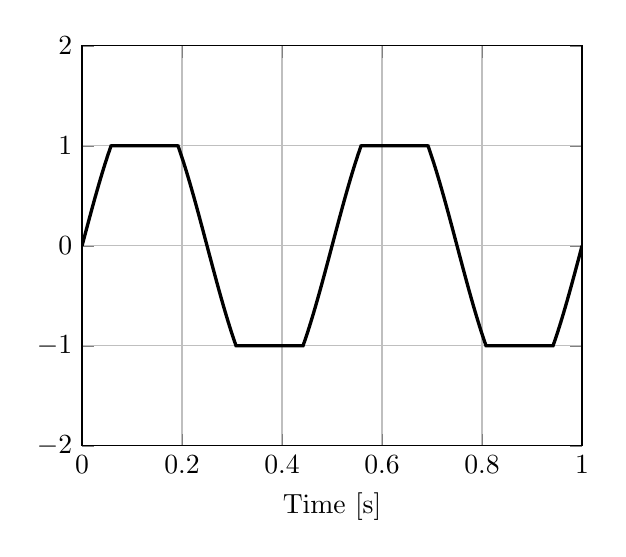
\begin{tikzpicture}

\begin{axis}[%
width=2.5in,
height=2in,
at={(1.011in,0.642in)},
scale only axis,
xmin=0,
xmax=1,
xlabel={Time [s]},
xmajorgrids,
ymin=-2,
ymax=2,
ymajorgrids,
axis background/.style={fill=white}
]
\addplot [color=black,solid,line width=1.2pt,forget plot]
  table[row sep=crcr]{%
0	0\\
0.001	0.0188490598250289\\
0.002	0.0376951431650062\\
0.003	0.0565352740049018\\
0.004	0.0753664772696543\\
0.005	0.0941857792939701\\
0.006	0.112990208291899\\
0.007	0.131776794826115\\
0.008	0.150542572276822\\
0.009	0.169284577310223\\
0.01	0.187999850346456\\
0.011	0.206685436026957\\
0.012	0.225338383681136\\
0.013	0.243955747792325\\
0.014	0.262534588462914\\
0.015	0.281071971878587\\
0.016	0.299564970771611\\
0.017	0.318010664883082\\
0.018	0.336406141424072\\
0.019	0.354748495535587\\
0.02	0.373034830747282\\
0.021	0.391262259434845\\
0.022	0.409427903275988\\
0.023	0.427528893704964\\
0.024	0.445562372365552\\
0.025	0.463525491562421\\
0.026	0.481415414710814\\
0.027	0.49922931678448\\
0.028	0.516964384761776\\
0.029	0.534617818069876\\
0.03	0.552186829027017\\
0.031	0.569668643282702\\
0.032	0.587060500255804\\
0.033	0.604359653570494\\
0.034	0.621563371489926\\
0.035	0.638668937347609\\
0.036	0.655673649976399\\
0.037	0.672574824135048\\
0.038	0.689369790932232\\
0.039	0.706055898247999\\
0.04	0.722630511152573\\
0.041	0.739091012322437\\
0.042	0.755434802453641\\
0.043	0.77165930067226\\
0.044	0.787761944941943\\
0.045	0.803740192468495\\
0.046	0.819591520101404\\
0.047	0.835313424732282\\
0.048	0.850903423690135\\
0.049	0.866359055133401\\
0.05	0.88167787843871\\
0.051	0.896857474586278\\
0.052	0.911895446541908\\
0.053	0.926789419635502\\
0.054	0.941537041936051\\
0.055	0.956135984623034\\
0.056	0.970583942354166\\
0.057	0.984878633629435\\
0.058	0.999017801151378\\
0.059	1\\
0.06	1\\
0.061	1\\
0.062	1\\
0.063	1\\
0.064	1\\
0.065	1\\
0.066	1\\
0.067	1\\
0.068	1\\
0.069	1\\
0.07	1\\
0.071	1\\
0.072	1\\
0.073	1\\
0.074	1\\
0.075	1\\
0.076	1\\
0.077	1\\
0.078	1\\
0.079	1\\
0.08	1\\
0.081	1\\
0.082	1\\
0.083	1\\
0.084	1\\
0.085	1\\
0.086	1\\
0.087	1\\
0.088	1\\
0.089	1\\
0.09	1\\
0.091	1\\
0.092	1\\
0.093	1\\
0.094	1\\
0.095	1\\
0.096	1\\
0.097	1\\
0.098	1\\
0.099	1\\
0.1	1\\
0.101	1\\
0.102	1\\
0.103	1\\
0.104	1\\
0.105	1\\
0.106	1\\
0.107	1\\
0.108	1\\
0.109	1\\
0.11	1\\
0.111	1\\
0.112	1\\
0.113	1\\
0.114	1\\
0.115	1\\
0.116	1\\
0.117	1\\
0.118	1\\
0.119	1\\
0.12	1\\
0.121	1\\
0.122	1\\
0.123	1\\
0.124	1\\
0.125	1\\
0.126	1\\
0.127	1\\
0.128	1\\
0.129	1\\
0.13	1\\
0.131	1\\
0.132	1\\
0.133	1\\
0.134	1\\
0.135	1\\
0.136	1\\
0.137	1\\
0.138	1\\
0.139	1\\
0.14	1\\
0.141	1\\
0.142	1\\
0.143	1\\
0.144	1\\
0.145	1\\
0.146	1\\
0.147	1\\
0.148	1\\
0.149	1\\
0.15	1\\
0.151	1\\
0.152	1\\
0.153	1\\
0.154	1\\
0.155	1\\
0.156	1\\
0.157	1\\
0.158	1\\
0.159	1\\
0.16	1\\
0.161	1\\
0.162	1\\
0.163	1\\
0.164	1\\
0.165	1\\
0.166	1\\
0.167	1\\
0.168	1\\
0.169	1\\
0.17	1\\
0.171	1\\
0.172	1\\
0.173	1\\
0.174	1\\
0.175	1\\
0.176	1\\
0.177	1\\
0.178	1\\
0.179	1\\
0.18	1\\
0.181	1\\
0.182	1\\
0.183	1\\
0.184	1\\
0.185	1\\
0.186	1\\
0.187	1\\
0.188	1\\
0.189	1\\
0.19	1\\
0.191	1\\
0.192	0.999017801151378\\
0.193	0.984878633629435\\
0.194	0.970583942354166\\
0.195	0.956135984623035\\
0.196	0.941537041936051\\
0.197	0.926789419635502\\
0.198	0.911895446541908\\
0.199	0.896857474586278\\
0.2	0.88167787843871\\
0.201	0.866359055133402\\
0.202	0.850903423690135\\
0.203	0.835313424732282\\
0.204	0.819591520101404\\
0.205	0.803740192468495\\
0.206	0.787761944941943\\
0.207	0.771659300672259\\
0.208	0.755434802453641\\
0.209	0.739091012322437\\
0.21	0.722630511152573\\
0.211	0.706055898247999\\
0.212	0.689369790932232\\
0.213	0.672574824135048\\
0.214	0.655673649976399\\
0.215	0.638668937347609\\
0.216	0.621563371489926\\
0.217	0.604359653570494\\
0.218	0.587060500255804\\
0.219	0.569668643282702\\
0.22	0.552186829027017\\
0.221	0.534617818069876\\
0.222	0.516964384761776\\
0.223	0.49922931678448\\
0.224	0.481415414710815\\
0.225	0.463525491562421\\
0.226	0.445562372365552\\
0.227	0.427528893704964\\
0.228	0.409427903275988\\
0.229	0.391262259434846\\
0.23	0.373034830747282\\
0.231	0.354748495535587\\
0.232	0.336406141424071\\
0.233	0.318010664883082\\
0.234	0.299564970771611\\
0.235	0.281071971878587\\
0.236	0.262534588462914\\
0.237	0.243955747792325\\
0.238	0.225338383681136\\
0.239	0.206685436026957\\
0.24	0.187999850346457\\
0.241	0.169284577310223\\
0.242	0.150542572276822\\
0.243	0.131776794826115\\
0.244	0.1129902082919\\
0.245	0.0941857792939704\\
0.246	0.0753664772696545\\
0.247	0.0565352740049018\\
0.248	0.0376951431650067\\
0.249	0.0188490598250293\\
0.25	1.83697019872103e-16\\
0.251	-0.0188490598250289\\
0.252	-0.0376951431650064\\
0.253	-0.0565352740049014\\
0.254	-0.0753664772696541\\
0.255	-0.09418577929397\\
0.256	-0.112990208291899\\
0.257	-0.131776794826114\\
0.258	-0.150542572276822\\
0.259	-0.169284577310222\\
0.26	-0.187999850346456\\
0.261	-0.206685436026957\\
0.262	-0.225338383681135\\
0.263	-0.243955747792325\\
0.264	-0.262534588462914\\
0.265	-0.281071971878587\\
0.266	-0.299564970771611\\
0.267	-0.318010664883082\\
0.268	-0.336406141424072\\
0.269	-0.354748495535587\\
0.27	-0.373034830747282\\
0.271	-0.391262259434845\\
0.272	-0.409427903275988\\
0.273	-0.427528893704964\\
0.274	-0.445562372365553\\
0.275	-0.463525491562422\\
0.276	-0.481415414710814\\
0.277	-0.49922931678448\\
0.278	-0.516964384761776\\
0.279	-0.534617818069876\\
0.28	-0.552186829027017\\
0.281	-0.569668643282702\\
0.282	-0.587060500255804\\
0.283	-0.604359653570494\\
0.284	-0.621563371489927\\
0.285	-0.638668937347609\\
0.286	-0.6556736499764\\
0.287	-0.672574824135049\\
0.288	-0.689369790932232\\
0.289	-0.706055898247998\\
0.29	-0.722630511152572\\
0.291	-0.739091012322437\\
0.292	-0.755434802453641\\
0.293	-0.771659300672259\\
0.294	-0.787761944941943\\
0.295	-0.803740192468495\\
0.296	-0.819591520101403\\
0.297	-0.835313424732281\\
0.298	-0.850903423690134\\
0.299	-0.866359055133401\\
0.3	-0.88167787843871\\
0.301	-0.896857474586278\\
0.302	-0.911895446541908\\
0.303	-0.926789419635501\\
0.304	-0.94153704193605\\
0.305	-0.956135984623034\\
0.306	-0.970583942354166\\
0.307	-0.984878633629434\\
0.308	-0.999017801151377\\
0.309	-1\\
0.31	-1\\
0.311	-1\\
0.312	-1\\
0.313	-1\\
0.314	-1\\
0.315	-1\\
0.316	-1\\
0.317	-1\\
0.318	-1\\
0.319	-1\\
0.32	-1\\
0.321	-1\\
0.322	-1\\
0.323	-1\\
0.324	-1\\
0.325	-1\\
0.326	-1\\
0.327	-1\\
0.328	-1\\
0.329	-1\\
0.33	-1\\
0.331	-1\\
0.332	-1\\
0.333	-1\\
0.334	-1\\
0.335	-1\\
0.336	-1\\
0.337	-1\\
0.338	-1\\
0.339	-1\\
0.34	-1\\
0.341	-1\\
0.342	-1\\
0.343	-1\\
0.344	-1\\
0.345	-1\\
0.346	-1\\
0.347	-1\\
0.348	-1\\
0.349	-1\\
0.35	-1\\
0.351	-1\\
0.352	-1\\
0.353	-1\\
0.354	-1\\
0.355	-1\\
0.356	-1\\
0.357	-1\\
0.358	-1\\
0.359	-1\\
0.36	-1\\
0.361	-1\\
0.362	-1\\
0.363	-1\\
0.364	-1\\
0.365	-1\\
0.366	-1\\
0.367	-1\\
0.368	-1\\
0.369	-1\\
0.37	-1\\
0.371	-1\\
0.372	-1\\
0.373	-1\\
0.374	-1\\
0.375	-1\\
0.376	-1\\
0.377	-1\\
0.378	-1\\
0.379	-1\\
0.38	-1\\
0.381	-1\\
0.382	-1\\
0.383	-1\\
0.384	-1\\
0.385	-1\\
0.386	-1\\
0.387	-1\\
0.388	-1\\
0.389	-1\\
0.39	-1\\
0.391	-1\\
0.392	-1\\
0.393	-1\\
0.394	-1\\
0.395	-1\\
0.396	-1\\
0.397	-1\\
0.398	-1\\
0.399	-1\\
0.4	-1\\
0.401	-1\\
0.402	-1\\
0.403	-1\\
0.404	-1\\
0.405	-1\\
0.406	-1\\
0.407	-1\\
0.408	-1\\
0.409	-1\\
0.41	-1\\
0.411	-1\\
0.412	-1\\
0.413	-1\\
0.414	-1\\
0.415	-1\\
0.416	-1\\
0.417	-1\\
0.418	-1\\
0.419	-1\\
0.42	-1\\
0.421	-1\\
0.422	-1\\
0.423	-1\\
0.424	-1\\
0.425	-1\\
0.426	-1\\
0.427	-1\\
0.428	-1\\
0.429	-1\\
0.43	-1\\
0.431	-1\\
0.432	-1\\
0.433	-1\\
0.434	-1\\
0.435	-1\\
0.436	-1\\
0.437	-1\\
0.438	-1\\
0.439	-1\\
0.44	-1\\
0.441	-1\\
0.442	-0.999017801151378\\
0.443	-0.984878633629435\\
0.444	-0.970583942354166\\
0.445	-0.956135984623034\\
0.446	-0.94153704193605\\
0.447	-0.926789419635502\\
0.448	-0.911895446541909\\
0.449	-0.896857474586279\\
0.45	-0.88167787843871\\
0.451	-0.866359055133402\\
0.452	-0.850903423690135\\
0.453	-0.835313424732282\\
0.454	-0.819591520101403\\
0.455	-0.803740192468494\\
0.456	-0.787761944941943\\
0.457	-0.77165930067226\\
0.458	-0.755434802453641\\
0.459	-0.739091012322437\\
0.46	-0.722630511152573\\
0.461	-0.706055898247999\\
0.462	-0.689369790932232\\
0.463	-0.672574824135048\\
0.464	-0.655673649976399\\
0.465	-0.638668937347608\\
0.466	-0.621563371489927\\
0.467	-0.604359653570494\\
0.468	-0.587060500255804\\
0.469	-0.569668643282702\\
0.47	-0.552186829027017\\
0.471	-0.534617818069876\\
0.472	-0.516964384761775\\
0.473	-0.499229316784479\\
0.474	-0.481415414710814\\
0.475	-0.463525491562421\\
0.476	-0.445562372365553\\
0.477	-0.427528893704964\\
0.478	-0.409427903275988\\
0.479	-0.391262259434845\\
0.48	-0.373034830747283\\
0.481	-0.354748495535588\\
0.482	-0.336406141424072\\
0.483	-0.318010664883082\\
0.484	-0.299564970771611\\
0.485	-0.281071971878587\\
0.486	-0.262534588462914\\
0.487	-0.243955747792326\\
0.488	-0.225338383681137\\
0.489	-0.206685436026958\\
0.49	-0.187999850346457\\
0.491	-0.169284577310223\\
0.492	-0.150542572276823\\
0.493	-0.131776794826115\\
0.494	-0.112990208291899\\
0.495	-0.0941857792939699\\
0.496	-0.0753664772696553\\
0.497	-0.0565352740049027\\
0.498	-0.0376951431650069\\
0.499	-0.0188490598250294\\
0.5	-3.67394039744206e-16\\
0.501	0.0188490598250287\\
0.502	0.0376951431650062\\
0.503	0.0565352740049019\\
0.504	0.0753664772696546\\
0.505	0.0941857792939692\\
0.506	0.112990208291898\\
0.507	0.131776794826114\\
0.508	0.150542572276822\\
0.509	0.169284577310222\\
0.51	0.187999850346456\\
0.511	0.206685436026957\\
0.512	0.225338383681136\\
0.513	0.243955747792326\\
0.514	0.262534588462913\\
0.515	0.281071971878586\\
0.516	0.29956497077161\\
0.517	0.318010664883082\\
0.518	0.336406141424072\\
0.519	0.354748495535587\\
0.52	0.373034830747282\\
0.521	0.391262259434843\\
0.522	0.409427903275988\\
0.523	0.427528893704962\\
0.524	0.445562372365552\\
0.525	0.46352549156242\\
0.526	0.481415414710814\\
0.527	0.499229316784479\\
0.528	0.516964384761776\\
0.529	0.534617818069874\\
0.53	0.552186829027017\\
0.531	0.5696686432827\\
0.532	0.587060500255804\\
0.533	0.604359653570492\\
0.534	0.621563371489926\\
0.535	0.638668937347608\\
0.536	0.655673649976399\\
0.537	0.672574824135046\\
0.538	0.689369790932232\\
0.539	0.706055898247997\\
0.54	0.722630511152573\\
0.541	0.739091012322436\\
0.542	0.755434802453641\\
0.543	0.771659300672258\\
0.544	0.787761944941944\\
0.545	0.803740192468494\\
0.546	0.819591520101404\\
0.547	0.83531342473228\\
0.548	0.850903423690135\\
0.549	0.8663590551334\\
0.55	0.88167787843871\\
0.551	0.896857474586277\\
0.552	0.911895446541908\\
0.553	0.9267894196355\\
0.554	0.941537041936051\\
0.555	0.956135984623034\\
0.556	0.970583942354167\\
0.557	0.984878633629433\\
0.558	0.999017801151378\\
0.559	1\\
0.56	1\\
0.561	1\\
0.562	1\\
0.563	1\\
0.564	1\\
0.565	1\\
0.566	1\\
0.567	1\\
0.568	1\\
0.569	1\\
0.57	1\\
0.571	1\\
0.572	1\\
0.573	1\\
0.574	1\\
0.575	1\\
0.576	1\\
0.577	1\\
0.578	1\\
0.579	1\\
0.58	1\\
0.581	1\\
0.582	1\\
0.583	1\\
0.584	1\\
0.585	1\\
0.586	1\\
0.587	1\\
0.588	1\\
0.589	1\\
0.59	1\\
0.591	1\\
0.592	1\\
0.593	1\\
0.594	1\\
0.595	1\\
0.596	1\\
0.597	1\\
0.598	1\\
0.599	1\\
0.6	1\\
0.601	1\\
0.602	1\\
0.603	1\\
0.604	1\\
0.605	1\\
0.606	1\\
0.607	1\\
0.608	1\\
0.609	1\\
0.61	1\\
0.611	1\\
0.612	1\\
0.613	1\\
0.614	1\\
0.615	1\\
0.616	1\\
0.617	1\\
0.618	1\\
0.619	1\\
0.62	1\\
0.621	1\\
0.622	1\\
0.623	1\\
0.624	1\\
0.625	1\\
0.626	1\\
0.627	1\\
0.628	1\\
0.629	1\\
0.63	1\\
0.631	1\\
0.632	1\\
0.633	1\\
0.634	1\\
0.635	1\\
0.636	1\\
0.637	1\\
0.638	1\\
0.639	1\\
0.64	1\\
0.641	1\\
0.642	1\\
0.643	1\\
0.644	1\\
0.645	1\\
0.646	1\\
0.647	1\\
0.648	1\\
0.649	1\\
0.65	1\\
0.651	1\\
0.652	1\\
0.653	1\\
0.654	1\\
0.655	1\\
0.656	1\\
0.657	1\\
0.658	1\\
0.659	1\\
0.66	1\\
0.661	1\\
0.662	1\\
0.663	1\\
0.664	1\\
0.665	1\\
0.666	1\\
0.667	1\\
0.668	1\\
0.669	1\\
0.67	1\\
0.671	1\\
0.672	1\\
0.673	1\\
0.674	1\\
0.675	1\\
0.676	1\\
0.677	1\\
0.678	1\\
0.679	1\\
0.68	1\\
0.681	1\\
0.682	1\\
0.683	1\\
0.684	1\\
0.685	1\\
0.686	1\\
0.687	1\\
0.688	1\\
0.689	1\\
0.69	1\\
0.691	1\\
0.692	0.999017801151379\\
0.693	0.984878633629435\\
0.694	0.970583942354168\\
0.695	0.956135984623035\\
0.696	0.941537041936052\\
0.697	0.926789419635501\\
0.698	0.911895446541909\\
0.699	0.896857474586278\\
0.7	0.88167787843871\\
0.701	0.866359055133401\\
0.702	0.850903423690135\\
0.703	0.835313424732281\\
0.704	0.819591520101406\\
0.705	0.803740192468493\\
0.706	0.787761944941945\\
0.707	0.771659300672258\\
0.708	0.755434802453643\\
0.709	0.739091012322438\\
0.71	0.722630511152574\\
0.711	0.706055898247999\\
0.712	0.689369790932233\\
0.713	0.672574824135051\\
0.714	0.6556736499764\\
0.715	0.638668937347611\\
0.716	0.621563371489927\\
0.717	0.604359653570496\\
0.718	0.587060500255804\\
0.719	0.569668643282703\\
0.72	0.552186829027017\\
0.721	0.534617818069877\\
0.722	0.516964384761775\\
0.723	0.499229316784481\\
0.724	0.481415414710816\\
0.725	0.463525491562422\\
0.726	0.445562372365554\\
0.727	0.427528893704964\\
0.728	0.409427903275989\\
0.729	0.391262259434845\\
0.73	0.373034830747283\\
0.731	0.354748495535587\\
0.732	0.336406141424072\\
0.733	0.318010664883084\\
0.734	0.299564970771611\\
0.735	0.281071971878589\\
0.736	0.262534588462914\\
0.737	0.243955747792327\\
0.738	0.225338383681135\\
0.739	0.206685436026958\\
0.74	0.187999850346456\\
0.741	0.169284577310223\\
0.742	0.150542572276824\\
0.743	0.131776794826115\\
0.744	0.112990208291901\\
0.745	0.0941857792939701\\
0.746	0.0753664772696555\\
0.747	0.0565352740049015\\
0.748	0.0376951431650071\\
0.749	0.0188490598250283\\
0.75	5.51091059616309e-16\\
0.751	-0.0188490598250272\\
0.752	-0.037695143165006\\
0.753	-0.0565352740049004\\
0.754	-0.0753664772696544\\
0.755	-0.094185779293969\\
0.756	-0.112990208291899\\
0.757	-0.131776794826114\\
0.758	-0.150542572276823\\
0.759	-0.169284577310222\\
0.76	-0.187999850346455\\
0.761	-0.206685436026957\\
0.762	-0.225338383681134\\
0.763	-0.243955747792326\\
0.764	-0.262534588462913\\
0.765	-0.281071971878587\\
0.766	-0.29956497077161\\
0.767	-0.318010664883083\\
0.768	-0.336406141424071\\
0.769	-0.354748495535586\\
0.77	-0.373034830747282\\
0.771	-0.391262259434844\\
0.772	-0.409427903275988\\
0.773	-0.427528893704963\\
0.774	-0.445562372365553\\
0.775	-0.463525491562421\\
0.776	-0.481415414710815\\
0.777	-0.49922931678448\\
0.778	-0.516964384761774\\
0.779	-0.534617818069876\\
0.78	-0.552186829027016\\
0.781	-0.569668643282702\\
0.782	-0.587060500255803\\
0.783	-0.604359653570495\\
0.784	-0.621563371489926\\
0.785	-0.63866893734761\\
0.786	-0.655673649976399\\
0.787	-0.67257482413505\\
0.788	-0.689369790932232\\
0.789	-0.706055898247998\\
0.79	-0.722630511152573\\
0.791	-0.739091012322437\\
0.792	-0.755434802453642\\
0.793	-0.771659300672257\\
0.794	-0.787761944941945\\
0.795	-0.803740192468493\\
0.796	-0.819591520101405\\
0.797	-0.83531342473228\\
0.798	-0.850903423690134\\
0.799	-0.8663590551334\\
0.8	-0.881677878438709\\
0.801	-0.896857474586277\\
0.802	-0.911895446541908\\
0.803	-0.9267894196355\\
0.804	-0.941537041936051\\
0.805	-0.956135984623034\\
0.806	-0.970583942354167\\
0.807	-0.984878633629434\\
0.808	-0.999017801151378\\
0.809	-1\\
0.81	-1\\
0.811	-1\\
0.812	-1\\
0.813	-1\\
0.814	-1\\
0.815	-1\\
0.816	-1\\
0.817	-1\\
0.818	-1\\
0.819	-1\\
0.82	-1\\
0.821	-1\\
0.822	-1\\
0.823	-1\\
0.824	-1\\
0.825	-1\\
0.826	-1\\
0.827	-1\\
0.828	-1\\
0.829	-1\\
0.83	-1\\
0.831	-1\\
0.832	-1\\
0.833	-1\\
0.834	-1\\
0.835	-1\\
0.836	-1\\
0.837	-1\\
0.838	-1\\
0.839	-1\\
0.84	-1\\
0.841	-1\\
0.842	-1\\
0.843	-1\\
0.844	-1\\
0.845	-1\\
0.846	-1\\
0.847	-1\\
0.848	-1\\
0.849	-1\\
0.85	-1\\
0.851	-1\\
0.852	-1\\
0.853	-1\\
0.854	-1\\
0.855	-1\\
0.856	-1\\
0.857	-1\\
0.858	-1\\
0.859	-1\\
0.86	-1\\
0.861	-1\\
0.862	-1\\
0.863	-1\\
0.864	-1\\
0.865	-1\\
0.866	-1\\
0.867	-1\\
0.868	-1\\
0.869	-1\\
0.87	-1\\
0.871	-1\\
0.872	-1\\
0.873	-1\\
0.874	-1\\
0.875	-1\\
0.876	-1\\
0.877	-1\\
0.878	-1\\
0.879	-1\\
0.88	-1\\
0.881	-1\\
0.882	-1\\
0.883	-1\\
0.884	-1\\
0.885	-1\\
0.886	-1\\
0.887	-1\\
0.888	-1\\
0.889	-1\\
0.89	-1\\
0.891	-1\\
0.892	-1\\
0.893	-1\\
0.894	-1\\
0.895	-1\\
0.896	-1\\
0.897	-1\\
0.898	-1\\
0.899	-1\\
0.9	-1\\
0.901	-1\\
0.902	-1\\
0.903	-1\\
0.904	-1\\
0.905	-1\\
0.906	-1\\
0.907	-1\\
0.908	-1\\
0.909	-1\\
0.91	-1\\
0.911	-1\\
0.912	-1\\
0.913	-1\\
0.914	-1\\
0.915	-1\\
0.916	-1\\
0.917	-1\\
0.918	-1\\
0.919	-1\\
0.92	-1\\
0.921	-1\\
0.922	-1\\
0.923	-1\\
0.924	-1\\
0.925	-1\\
0.926	-1\\
0.927	-1\\
0.928	-1\\
0.929	-1\\
0.93	-1\\
0.931	-1\\
0.932	-1\\
0.933	-1\\
0.934	-1\\
0.935	-1\\
0.936	-1\\
0.937	-1\\
0.938	-1\\
0.939	-1\\
0.94	-1\\
0.941	-1\\
0.942	-0.999017801151379\\
0.943	-0.984878633629435\\
0.944	-0.970583942354168\\
0.945	-0.956135984623037\\
0.946	-0.941537041936052\\
0.947	-0.926789419635504\\
0.948	-0.911895446541909\\
0.949	-0.89685747458628\\
0.95	-0.88167787843871\\
0.951	-0.866359055133403\\
0.952	-0.850903423690135\\
0.953	-0.835313424732283\\
0.954	-0.819591520101406\\
0.955	-0.803740192468496\\
0.956	-0.787761944941946\\
0.957	-0.771659300672261\\
0.958	-0.755434802453643\\
0.959	-0.739091012322438\\
0.96	-0.722630511152574\\
0.961	-0.706055898247999\\
0.962	-0.689369790932233\\
0.963	-0.672574824135051\\
0.964	-0.6556736499764\\
0.965	-0.638668937347611\\
0.966	-0.621563371489927\\
0.967	-0.604359653570496\\
0.968	-0.587060500255804\\
0.969	-0.569668643282703\\
0.97	-0.552186829027017\\
0.971	-0.534617818069877\\
0.972	-0.516964384761775\\
0.973	-0.499229316784481\\
0.974	-0.481415414710816\\
0.975	-0.463525491562422\\
0.976	-0.445562372365554\\
0.977	-0.427528893704965\\
0.978	-0.409427903275989\\
0.979	-0.391262259434845\\
0.98	-0.373034830747283\\
0.981	-0.354748495535587\\
0.982	-0.336406141424073\\
0.983	-0.318010664883084\\
0.984	-0.299564970771611\\
0.985	-0.281071971878589\\
0.986	-0.262534588462914\\
0.987	-0.243955747792327\\
0.988	-0.225338383681136\\
0.989	-0.206685436026958\\
0.99	-0.187999850346456\\
0.991	-0.169284577310223\\
0.992	-0.150542572276824\\
0.993	-0.131776794826115\\
0.994	-0.112990208291901\\
0.995	-0.0941857792939703\\
0.996	-0.0753664772696557\\
0.997	-0.0565352740049017\\
0.998	-0.0376951431650073\\
0.999	-0.0188490598250285\\
1	-7.34788079488412e-16\\
};
\end{axis}
\end{tikzpicture}%
	\caption{A 1 kHz clipped sinusoid.}
	\label{fig:clippingDist}
\end{subfigure}
\caption{The difference between a unaffected signal and a clipped signal. As the maximum output is 1, the signal is hard clipped because of the limitation.}
\label{fig:audioclipping}
\end{figure}

Hard clipping lowers the sound quality if the clipping is not intended, and should therefore be avoided. The wave distortion created by the sharp edge results in a square-wave-like signal. This creates additional uneven harmonics to the signal i.e. 3rd, 5th, 7th and 9th, which are unpleasant to listen to as previously stated. Since the clipping creates the square-wave-like signal, the generation of the additional uneven harmonics can be described in the Fourier series of a square-wave. The Fourier series of a square-wave is given as:
\begin{align}\label{eq:fourier_series_square}
f(t) &= \frac{4}{\pi} \sum_{n=1}^{\infty} \frac{\sin (\omega_0 t \cdot (2n-1))}{(2n-1)} \\
	 &= \frac{4}{\pi} (\sin(\omega_0 t) + \frac{1}{3}\sin(3 \omega_0 t) + \frac{1}{5}\sin(5 \omega_0 t) + \, ... \,)
\end{align}
\begin{where}
\va{$\omega_0$}{is the fundamental frequency of the square-wave.}{rad/s}\\
\end{where}

As seen in \autoref{eq:fourier_series_square}, the function of a square-wave signal consists of a fundamental frequency $\omega_0$ and uneven harmonics to the fundamental frequency. This can also be shown in a spectrum analysis of the 1 kHz clipped sinusoid from \autoref{fig:audioclipping} in \autoref{fig:audioclippingFFT}.

\begin{figure}[H]
\centering
\begin{subfigure}[t]{0.47\textwidth}
	\tikzsetnextfilename{clippingCleanFFT}
	% This file was created by matlab2tikz.
%
%The latest updates can be retrieved from
%  http://www.mathworks.com/matlabcentral/fileexchange/22022-matlab2tikz-matlab2tikz
%where you can also make suggestions and rate matlab2tikz.
%
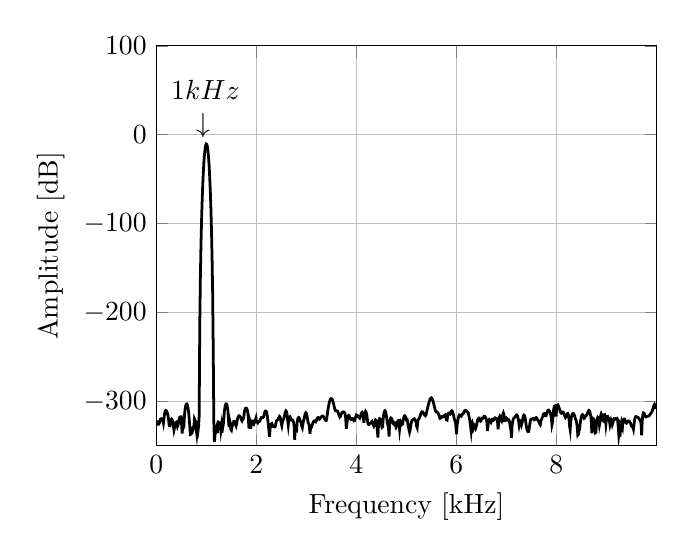
\begin{tikzpicture}

\begin{axis}[%
width=2.5in,
height=2in,
at={(1.011in,0.642in)},
scale only axis,
scaled x ticks = false,
xmin=0,
xmax=10000,
xlabel={Frequency [kHz]},
xmajorgrids,
ymin=-350,
ymax=100,
xticklabels={0, 2, 4, 6, 8},
xtick = {0, 2000, 4000, 6000, 8000},
ylabel={Amplitude [dB]},
ymajorgrids,
axis background/.style={fill=white},
]
\addplot [color=black,solid,line width=1pt,forget plot]
  table[row sep=crcr]{%
0	-322.11596721008\\
11.7216117216117	-323.671020481401\\
23.4432234432234	-323.340883337027\\
35.1648351648352	-325.684167070818\\
46.8864468864469	-325.669523756719\\
58.6080586080586	-324.370513022472\\
70.3296703296703	-322.159992029701\\
82.0512820512821	-319.994159311925\\
93.7728937728938	-319.483979753379\\
105.494505494505	-319.494939928451\\
117.216117216117	-320.869322942301\\
128.937728937729	-320.920572736749\\
140.659340659341	-324.227184829387\\
152.380952380952	-319.035056899834\\
164.102564102564	-313.823145631125\\
175.824175824176	-311.131574765862\\
187.545787545788	-310.246860211816\\
199.267399267399	-310.60441452423\\
210.989010989011	-311.78696455392\\
222.710622710623	-313.844752745052\\
234.432234432234	-316.418042709319\\
246.153846153846	-321.707697545501\\
257.875457875458	-327.363976836631\\
269.59706959707	-327.473089119894\\
281.318681318681	-324.112892105008\\
293.040293040293	-320.977587207666\\
304.761904761905	-319.982762533596\\
316.483516483516	-320.780760736175\\
328.205128205128	-323.668423270885\\
339.92673992674	-328.026148757277\\
351.648351648352	-332.4170697972\\
363.369963369963	-329.426095087341\\
375.091575091575	-326.556664292431\\
386.813186813187	-323.76537835188\\
398.534798534799	-323.368319264645\\
410.25641025641	-325.169104300057\\
421.978021978022	-328.189262138342\\
433.699633699634	-326.529217054039\\
445.421245421245	-322.75486943378\\
457.142857142857	-319.794087491908\\
468.864468864469	-317.719335966222\\
480.586080586081	-317.459852846429\\
492.307692307692	-319.009687543967\\
504.029304029304	-325.455766258282\\
515.750915750916	-336.106317374067\\
527.472527472527	-326.323603862667\\
539.194139194139	-329.684995875921\\
550.915750915751	-327.90212185778\\
562.637362637363	-314.792259957384\\
574.358974358974	-308.679273562794\\
586.080586080586	-304.859856763288\\
597.802197802198	-303.147924647545\\
609.52380952381	-302.958088372619\\
621.245421245421	-304.246172084633\\
632.967032967033	-307.392871145609\\
644.688644688645	-311.86240623327\\
656.410256410256	-319.720154828058\\
668.131868131868	-327.681235000644\\
679.85347985348	-337.238516322602\\
691.575091575092	-336.970257356979\\
703.296703296703	-332.332133924419\\
715.018315018315	-331.141735134048\\
726.739926739927	-332.723957001084\\
738.461538461538	-330.730504488432\\
750.18315018315	-327.778175020515\\
761.904761904762	-319.91378584982\\
773.626373626374	-321.461497849882\\
785.347985347985	-327.043537773181\\
797.069597069597	-331.841589615916\\
808.791208791209	-336.991655282628\\
820.512820512821	-330.418202230553\\
832.234432234432	-333.267393421045\\
843.956043956044	-328.226187037683\\
855.677655677656	-316.700315440438\\
867.399267399267	-215.943651772091\\
879.120879120879	-163.159584780945\\
890.842490842491	-126.529341228273\\
902.564102564103	-98.3775899142248\\
914.285714285714	-75.9321258862354\\
926.007326007326	-57.8132086793137\\
937.728937728938	-43.2219634542571\\
949.450549450549	-31.6552033180823\\
961.172161172161	-22.7812801668732\\
972.893772893773	-16.3785078578736\\
984.615384615385	-12.3020988974321\\
996.336996336996	-10.4658259320985\\
1008.05860805861	-10.8322625838136\\
1019.78021978022	-13.4088092670734\\
1031.50183150183	-18.2484666216626\\
1043.22344322344	-25.4555537550734\\
1054.94505494505	-35.1978991745999\\
1066.66666666667	-47.7291574398437\\
1078.38827838828	-63.4292414488433\\
1090.10989010989	-82.8812589369107\\
1101.8315018315	-107.032465507491\\
1113.55311355311	-137.586526131487\\
1125.27472527473	-178.243096713105\\
1136.99633699634	-241.704411925533\\
1148.71794871795	-323.195571130692\\
1160.43956043956	-345.375156099691\\
1172.16117216117	-338.247857244841\\
1183.88278388278	-333.32317434497\\
1195.6043956044	-331.269745255181\\
1207.32600732601	-328.799242404036\\
1219.04761904762	-335.934946361628\\
1230.76923076923	-327.685186138873\\
1242.49084249084	-326.960459897927\\
1254.21245421245	-323.718010447396\\
1265.93406593407	-324.108622411667\\
1277.65567765568	-326.20417623814\\
1289.37728937729	-332.697946725791\\
1301.0989010989	-327.906853738375\\
1312.82051282051	-335.418538359777\\
1324.54212454212	-328.816875760217\\
1336.26373626374	-327.262600955998\\
1347.98534798535	-320.385055874777\\
1359.70695970696	-311.475672251247\\
1371.42857142857	-306.643481149913\\
1383.15018315018	-303.695848832502\\
1394.87179487179	-302.842835407919\\
1406.59340659341	-303.232099162736\\
1418.31501831502	-305.842604461406\\
1430.03663003663	-310.40119194813\\
1441.75824175824	-320.718788147534\\
1453.47985347985	-328.69918849089\\
1465.20146520147	-321.407968983388\\
1476.92307692308	-324.473146768564\\
1488.64468864469	-331.645069484275\\
1500.3663003663	-332.515642341006\\
1512.08791208791	-328.465510911873\\
1523.80952380952	-326.826340274793\\
1535.53113553114	-324.534133776849\\
1547.25274725275	-322.615676311941\\
1558.97435897436	-322.427557967468\\
1570.69597069597	-323.530722159417\\
1582.41758241758	-326.171996895262\\
1594.13919413919	-327.712500269681\\
1605.86080586081	-325.047841087069\\
1617.58241758242	-321.24290571993\\
1629.30402930403	-317.993077517342\\
1641.02564102564	-316.998612276315\\
1652.74725274725	-316.240926477532\\
1664.46886446886	-316.68363443687\\
1676.19047619048	-317.141867195876\\
1687.91208791209	-318.342449097449\\
1699.6336996337	-320.695345632283\\
1711.35531135531	-321.836458347942\\
1723.07692307692	-320.2697737784\\
1734.79853479853	-320.163464706646\\
1746.52014652015	-317.872908059459\\
1758.24175824176	-312.6677675311\\
1769.96336996337	-309.491750132905\\
1781.68498168498	-307.828765413517\\
1793.40659340659	-307.627883691429\\
1805.12820512821	-307.890708550761\\
1816.84981684982	-309.331169961249\\
1828.57142857143	-312.28725024046\\
1840.29304029304	-320.344727197184\\
1852.01465201465	-330.483981414598\\
1863.73626373626	-320.778838487233\\
1875.45787545788	-323.188753718667\\
1887.17948717949	-330.709648822314\\
1898.9010989011	-324.458698904598\\
1910.62271062271	-322.161594474234\\
1922.34432234432	-322.355261648298\\
1934.06593406593	-325.120354775896\\
1945.78754578755	-325.813966972437\\
1957.50915750916	-323.880005799796\\
1969.23076923077	-321.560515034589\\
1980.95238095238	-321.471577902989\\
1992.67399267399	-319.02446157723\\
2004.3956043956	-323.174195056939\\
2016.11721611722	-323.174195056939\\
2027.83882783883	-324.089344868152\\
2039.56043956044	-322.910905669715\\
2051.28205128205	-323.043188327053\\
2063.00366300366	-322.552600066038\\
2074.72527472527	-320.986469744908\\
2086.44688644689	-319.545996905778\\
2098.1684981685	-318.315254794156\\
2109.89010989011	-318.387111906887\\
2121.61172161172	-318.301603114866\\
2133.33333333333	-318.177294354268\\
2145.05494505495	-316.938934301122\\
2156.77655677656	-314.354332026841\\
2168.49816849817	-312.152839226024\\
2180.21978021978	-310.876376782709\\
2191.94139194139	-310.8442203955\\
2203.663003663	-312.377716587324\\
2215.38461538462	-315.505766578087\\
2227.10622710623	-320.600055628699\\
2238.82783882784	-326.363108229676\\
2250.54945054945	-332.879313477263\\
2262.27106227106	-339.927557268938\\
2273.99267399267	-330.784134841474\\
2285.71428571429	-326.949066776775\\
2297.4358974359	-325.310562015324\\
2309.15750915751	-324.900671542525\\
2320.87912087912	-326.68176647539\\
2332.60073260073	-328.158338680386\\
2344.32234432234	-328.204122091938\\
2356.04395604396	-328.051439236523\\
2367.76556776557	-328.664204937443\\
2379.48717948718	-328.099018637999\\
2391.20879120879	-324.310047965675\\
2402.9304029304	-321.667678539627\\
2414.65201465201	-321.135207214597\\
2426.37362637363	-320.880932262159\\
2438.09523809524	-319.778960318202\\
2449.81684981685	-317.987700465117\\
2461.53846153846	-316.78808552065\\
2473.26007326007	-317.473390142408\\
2484.98168498168	-320.222893879042\\
2496.7032967033	-324.854050216358\\
2508.42490842491	-327.365492440596\\
2520.14652014652	-323.224999893465\\
2531.86813186813	-321.091227031284\\
2543.58974358974	-320.156669708411\\
2555.31135531136	-317.840663339711\\
2567.03296703297	-314.501482216247\\
2578.75457875458	-311.854837339112\\
2590.47619047619	-310.724997354159\\
2602.1978021978	-311.622091427549\\
2613.91941391941	-314.851882898182\\
2625.64102564103	-321.512762623562\\
2637.36263736264	-326.715257821487\\
2649.08424908425	-320.965390398505\\
2660.80586080586	-318.299218269644\\
2672.52747252747	-317.485994241431\\
2684.24908424908	-318.59001422949\\
2695.9706959707	-320.576544514212\\
2707.69230769231	-321.22124456977\\
2719.41391941392	-321.571973538176\\
2731.13553113553	-321.42734530042\\
2742.85714285714	-323.182504523745\\
2754.57875457875	-327.818517304439\\
2766.30036630037	-343.340028971303\\
2778.02197802198	-328.590941502845\\
2789.74358974359	-329.209198839045\\
2801.4652014652	-335.009194971263\\
2813.18681318681	-324.917874359001\\
2824.90842490842	-320.675970970006\\
2836.63003663004	-318.598485286378\\
2848.35164835165	-318.175277091238\\
2860.07326007326	-318.965978881077\\
2871.79487179487	-320.835410347703\\
2883.51648351648	-322.524929825596\\
2895.2380952381	-324.578193849772\\
2906.95970695971	-327.880455873337\\
2918.68131868132	-329.561603057853\\
2930.40293040293	-325.490736098095\\
2942.12454212454	-322.172446534305\\
2953.84615384615	-319.538366387325\\
2965.56776556777	-316.454951611266\\
2977.28937728938	-313.715712999263\\
2989.01098901099	-312.765011451191\\
3000.7326007326	-313.550082053352\\
3012.45421245421	-316.332919236015\\
3024.17582417582	-320.464673621591\\
3035.89743589744	-324.21570173302\\
3047.61904761905	-325.14025136414\\
3059.34065934066	-328.179012620665\\
3071.06227106227	-336.319390511434\\
3082.78388278388	-330.540376761589\\
3094.50549450549	-328.055385719859\\
3106.22710622711	-328.41132792291\\
3117.94871794872	-326.398110320453\\
3129.67032967033	-324.429933801343\\
3141.39194139194	-322.958523531653\\
3153.11355311355	-322.080283026816\\
3164.83516483516	-321.986069592074\\
3176.55677655678	-322.88974461944\\
3188.27838827839	-323.14866547361\\
3200	-321.731991922314\\
3211.72161172161	-319.583271135606\\
3223.44322344322	-318.524693510682\\
3235.16483516484	-318.277835267365\\
3246.88644688645	-319.493530184348\\
3258.60805860806	-320.194783095862\\
3270.32967032967	-319.645880585364\\
3282.05128205128	-318.402355114397\\
3293.77289377289	-317.597734351514\\
3305.49450549451	-317.02187364446\\
3317.21611721612	-316.763942230905\\
3328.93772893773	-316.47058612926\\
3340.65934065934	-317.197718055388\\
3352.38095238095	-318.34030296296\\
3364.10256410256	-319.71475362671\\
3375.82417582418	-320.433372545647\\
3387.54578754579	-321.481423753538\\
3399.2673992674	-321.328758210847\\
3410.98901098901	-317.848121944058\\
3422.71062271062	-312.6052633917\\
3434.43223443223	-308.209983131555\\
3446.15384615385	-304.542297484367\\
3457.87545787546	-301.476640468968\\
3469.59706959707	-299.074162567864\\
3481.31868131868	-297.505270833626\\
3493.04029304029	-296.820826693279\\
3504.7619047619	-296.952977362533\\
3516.48351648352	-297.832794363821\\
3528.20512820513	-299.532668899083\\
3539.92673992674	-301.925997253397\\
3551.64835164835	-304.833072981485\\
3563.36996336996	-307.679247836289\\
3575.09157509158	-309.820085030418\\
3586.81318681319	-310.691494738001\\
3598.5347985348	-310.817398824033\\
3610.25641025641	-310.678764468745\\
3621.97802197802	-310.904852964739\\
3633.69963369963	-312.083008289962\\
3645.42124542125	-314.044889957489\\
3657.14285714286	-316.283113404039\\
3668.86446886447	-317.725995742272\\
3680.58608058608	-316.98711432429\\
3692.30769230769	-315.404661196974\\
3704.0293040293	-313.574046253917\\
3715.75091575092	-312.403769243541\\
3727.47252747253	-311.900292301962\\
3739.19413919414	-311.790821532916\\
3750.91575091575	-311.885255334962\\
3762.63736263736	-312.507671076698\\
3774.35897435897	-314.393900840475\\
3786.08058608059	-318.958623783513\\
3797.8021978022	-330.766521534997\\
3809.52380952381	-325.502820472922\\
3821.24542124542	-319.47490837836\\
3832.96703296703	-316.5879349607\\
3844.68864468864	-315.820977290156\\
3856.41025641026	-316.165835542033\\
3868.13186813187	-317.693295629945\\
3879.85347985348	-319.724105063858\\
3891.57509157509	-320.385668853013\\
3903.2967032967	-319.982487927687\\
3915.01831501832	-319.299311012412\\
3926.73992673993	-319.444342321726\\
3938.46153846154	-320.526575483676\\
3950.18315018315	-321.926779712727\\
3961.90476190476	-321.781804018036\\
3973.62637362637	-319.294600071473\\
3985.34798534799	-317.199406352915\\
3997.0695970696	-315.48532686416\\
4008.79120879121	-316.133918462084\\
4020.51282051282	-315.922088122408\\
4032.23443223443	-316.716666209588\\
4043.95604395604	-317.865988888969\\
4055.67765567766	-318.280559925241\\
4067.39926739927	-318.926776854331\\
4079.12087912088	-317.317696380994\\
4090.84249084249	-315.060841214154\\
4102.5641025641	-312.993854282692\\
4114.28571428571	-312.27769957935\\
4126.00732600733	-313.058993411349\\
4137.72893772894	-316.497495126966\\
4149.45054945055	-324.074551114817\\
4161.17216117216	-317.815498249607\\
4172.89377289377	-312.724221795712\\
4184.61538461538	-311.184304154482\\
4196.336996337	-312.180395095067\\
4208.05860805861	-315.33167553721\\
4219.78021978022	-320.223371703619\\
4231.50183150183	-324.981894832223\\
4243.22344322344	-325.968094640368\\
4254.94505494505	-325.975199382868\\
4266.66666666667	-325.044494992807\\
4278.38827838828	-324.748701483869\\
4290.10989010989	-324.298796557654\\
4301.8315018315	-323.185408013847\\
4313.55311355311	-322.493712256323\\
4325.27472527472	-324.004517791407\\
4336.99633699634	-326.395781230683\\
4348.71794871795	-327.81152123793\\
4360.43956043956	-326.215243804676\\
4372.16117216117	-323.991135829513\\
4383.88278388278	-320.982207180012\\
4395.6043956044	-321.462465973861\\
4407.32600732601	-324.176499385288\\
4419.04761904762	-332.267280302068\\
4430.76923076923	-340.80932861649\\
4442.49084249084	-326.258684322367\\
4454.21245421245	-321.442965268777\\
4465.93406593407	-319.544444432877\\
4477.65567765568	-320.026440215285\\
4489.37728937729	-321.870034014714\\
4501.0989010989	-325.275880091975\\
4512.82051282051	-329.135133788708\\
4524.54212454212	-328.535733131409\\
4536.26373626374	-319.872005913471\\
4547.98534798535	-314.353155551714\\
4559.70695970696	-311.431276989024\\
4571.42857142857	-310.598208874572\\
4583.15018315018	-311.541465335688\\
4594.87179487179	-314.262904844306\\
4606.59340659341	-318.957659426667\\
4618.31501831502	-324.341801794823\\
4630.03663003663	-326.908025760342\\
4641.75824175824	-329.671708602847\\
4653.47985347985	-339.598374824666\\
4665.20146520146	-324.239834487312\\
4676.92307692308	-320.142812870027\\
4688.64468864469	-318.579390590904\\
4700.3663003663	-318.904551228728\\
4712.08791208791	-320.164411571421\\
4723.80952380952	-323.552244720139\\
4735.53113553114	-325.133901656344\\
4747.25274725275	-325.67494410303\\
4758.97435897436	-323.730925971029\\
4770.69597069597	-324.141194152127\\
4782.41758241758	-327.036177280335\\
4794.13919413919	-329.052455856504\\
4805.86080586081	-327.62366085932\\
4817.58241758242	-324.243757917428\\
4829.30402930403	-321.85425099731\\
4841.02564102564	-321.644312334699\\
4852.74725274725	-324.65913326885\\
4864.46886446886	-331.375490539255\\
4876.19047619048	-325.679255623113\\
4887.91208791209	-322.838347325296\\
4899.6336996337	-323.86912625874\\
4911.35531135531	-326.111153620671\\
4923.07692307692	-325.63048628826\\
4934.79853479854	-321.471648674554\\
4946.52014652015	-318.118465437495\\
4958.24175824176	-316.68211874222\\
4969.96336996337	-316.211579968543\\
4981.68498168498	-317.228440996576\\
4993.40659340659	-319.26351539118\\
5005.12820512821	-321.443807346433\\
5016.84981684982	-321.020667676622\\
5028.57142857143	-324.31969794583\\
5040.29304029304	-328.84177524509\\
5052.01465201465	-331.83382615458\\
5063.73626373626	-334.735835579055\\
5075.45787545788	-332.299258886241\\
5087.17948717949	-327.630942194737\\
5098.9010989011	-323.781987640664\\
5110.62271062271	-321.395765925455\\
5122.34432234432	-320.886447997559\\
5134.06593406593	-320.465428875501\\
5145.78754578755	-319.820250617952\\
5157.50915750916	-319.568122144542\\
5169.23076923077	-320.445377078076\\
5180.95238095238	-321.775888699888\\
5192.67399267399	-323.327196438195\\
5204.3956043956	-327.748774429116\\
5216.11721611722	-329.500414479457\\
5227.83882783883	-322.930677708616\\
5239.56043956044	-320.345390384961\\
5251.28205128205	-319.46742292498\\
5263.00366300366	-318.422700195226\\
5274.72527472528	-316.460548794413\\
5286.44688644689	-314.420570373633\\
5298.1684981685	-312.634917234304\\
5309.89010989011	-311.645830096681\\
5321.61172161172	-311.606321565998\\
5333.33333333333	-312.395026397497\\
5345.05494505495	-313.644669672522\\
5356.77655677656	-314.764393688141\\
5368.49816849817	-315.637442053714\\
5380.21978021978	-316.335135300277\\
5391.94139194139	-315.462866674828\\
5403.663003663	-312.472956024358\\
5415.38461538462	-309.49096542544\\
5427.10622710623	-306.661910098118\\
5438.82783882784	-304.082440188536\\
5450.54945054945	-301.618020574783\\
5462.27106227106	-299.473868003226\\
5473.99267399267	-297.699114290504\\
5485.71428571429	-296.505406176026\\
5497.4358974359	-296.028411377836\\
5509.15750915751	-296.481646635714\\
5520.87912087912	-297.788088059893\\
5532.60073260073	-299.767551285277\\
5544.32234432234	-302.299391403697\\
5556.04395604396	-305.019492670558\\
5567.76556776557	-307.832948492747\\
5579.48717948718	-310.176717152399\\
5591.20879120879	-311.537518356175\\
5602.9304029304	-312.01745525393\\
5614.65201465201	-312.046097429218\\
5626.37362637363	-312.503028224505\\
5638.09523809524	-313.577705423825\\
5649.81684981685	-315.357798221399\\
5661.53846153846	-317.508009492954\\
5673.26007326007	-319.196199557734\\
5684.98168498169	-318.94203762454\\
5696.7032967033	-317.879613158787\\
5708.42490842491	-316.798370316049\\
5720.14652014652	-316.82023072804\\
5731.86813186813	-317.520829533155\\
5743.58974358974	-317.470921782045\\
5755.31135531136	-316.636505065392\\
5767.03296703297	-315.48666870282\\
5778.75457875458	-315.086859657696\\
5790.47619047619	-316.558142674321\\
5802.1978021978	-320.779865087743\\
5813.91941391941	-321.054678726594\\
5825.64102564103	-316.14666429264\\
5837.36263736264	-313.693752780448\\
5849.08424908425	-313.306516635395\\
5860.80586080586	-313.996318878861\\
5872.52747252747	-314.37620671086\\
5884.24908424908	-313.166557488194\\
5895.9706959707	-311.376347149641\\
5907.69230769231	-310.609368275481\\
5919.41391941392	-311.055178949651\\
5931.13553113553	-312.880034391828\\
5942.85714285714	-315.651542934863\\
5954.57875457875	-318.878501759082\\
5966.30036630037	-321.036914294143\\
5978.02197802198	-322.640785223042\\
5989.74358974359	-327.717946996982\\
6001.4652014652	-336.905142623736\\
6013.18681318681	-327.005050138264\\
6024.90842490843	-322.811148168367\\
6036.63003663004	-319.380448937682\\
6048.35164835165	-316.788794523067\\
6060.07326007326	-315.260026736671\\
6071.79487179487	-315.500235117214\\
6083.51648351648	-316.31262723076\\
6095.2380952381	-316.737763870142\\
6106.95970695971	-315.570585456679\\
6118.68131868132	-314.512473865216\\
6130.40293040293	-314.136967184497\\
6142.12454212454	-313.29777999593\\
6153.84615384615	-311.709230965213\\
6165.56776556777	-310.49076173709\\
6177.28937728938	-310.045515193581\\
6189.01098901099	-310.246728483171\\
6200.7326007326	-310.787694641331\\
6212.45421245421	-311.176489009487\\
6224.17582417582	-311.809877276123\\
6235.89743589744	-313.113077702783\\
6247.61904761905	-315.616909829523\\
6259.34065934066	-318.661714183517\\
6271.06227106227	-322.313080483317\\
6282.78388278388	-327.918824513223\\
6294.50549450549	-333.109040304427\\
6306.22710622711	-325.927465960554\\
6317.94871794872	-323.996489833835\\
6329.67032967033	-326.273728960488\\
6341.39194139194	-330.315574560491\\
6353.11355311355	-328.483366853066\\
6364.83516483516	-326.74920929609\\
6376.55677655678	-327.49073574341\\
6388.27838827839	-329.789351229632\\
6400	-327.930813274501\\
6411.72161172161	-324.610485895231\\
6423.44322344322	-321.167986704039\\
6435.16483516484	-319.665930677914\\
6446.88644688645	-319.111410353944\\
6458.60805860806	-320.364903454833\\
6470.32967032967	-321.914877776708\\
6482.05128205128	-322.313799686604\\
6493.77289377289	-321.740312795319\\
6505.49450549451	-319.296121098251\\
6517.21611721612	-319.69294349133\\
6528.93772893773	-318.952028639534\\
6540.65934065934	-318.501704630851\\
6552.38095238095	-316.777475572032\\
6564.10256410256	-316.717006826668\\
6575.82417582418	-317.61125822692\\
6587.54578754579	-318.786507250062\\
6599.2673992674	-320.239735171892\\
6610.98901098901	-324.104041604204\\
6622.71062271062	-333.35063319449\\
6634.43223443223	-326.537528631427\\
6646.15384615385	-321.590163141839\\
6657.87545787546	-320.404503211436\\
6669.59706959707	-321.094255003877\\
6681.31868131868	-322.52941342568\\
6693.04029304029	-323.673564331662\\
6704.7619047619	-322.201692071793\\
6716.48351648352	-320.244858854374\\
6728.20512820513	-320.251901048602\\
6739.92673992674	-321.35689658538\\
6751.64835164835	-320.990179578456\\
6763.36996336996	-319.060876489788\\
6775.09157509157	-318.533942823261\\
6786.81318681319	-318.916808430597\\
6798.5347985348	-319.518804604868\\
6810.25641025641	-319.924529824657\\
6821.97802197802	-321.980145450263\\
6833.69963369963	-331.458275918032\\
6845.42124542125	-324.125151967631\\
6857.14285714286	-317.900153356718\\
6868.86446886447	-316.689697147324\\
6880.58608058608	-317.850204581596\\
6892.30769230769	-320.962901491635\\
6904.0293040293	-322.04501633756\\
6915.75091575092	-319.148423142536\\
6927.47252747253	-314.712507000867\\
6939.19413919414	-312.955201335434\\
6950.91575091575	-314.934438338139\\
6962.63736263736	-321.691805921343\\
6974.35897435897	-321.507416252971\\
6986.08058608059	-318.913831166071\\
6997.8021978022	-318.537296556117\\
7009.52380952381	-319.664940734387\\
7021.24542124542	-321.033184631024\\
7032.96703296703	-321.280597507472\\
7044.68864468864	-320.65348783344\\
7056.41025641026	-321.544268892108\\
7068.13186813187	-324.909985331434\\
7079.85347985348	-329.313186838791\\
7091.57509157509	-332.280661546479\\
7103.2967032967	-341.061236750148\\
7115.01831501831	-326.69538279765\\
7126.73992673993	-322.292835964636\\
7138.46153846154	-319.989311376396\\
7150.18315018315	-318.630002550268\\
7161.90476190476	-318.245973589254\\
7173.62637362637	-317.726642570322\\
7185.34798534799	-316.718635481522\\
7197.0695970696	-315.563757275132\\
7208.79120879121	-315.241824611678\\
7220.51282051282	-316.080440447667\\
7232.23443223443	-318.468702319092\\
7243.95604395604	-322.360684600848\\
7255.67765567766	-327.075552711074\\
7267.39926739927	-324.075922278487\\
7279.12087912088	-322.751656854546\\
7290.84249084249	-323.770874889428\\
7302.5641025641	-326.404213176727\\
7314.28571428571	-324.276513906979\\
7326.00732600733	-319.604985711716\\
7337.72893772894	-316.885227851634\\
7349.45054945055	-315.509440863834\\
7361.17216117216	-315.885980380922\\
7372.89377289377	-317.869887758875\\
7384.61538461538	-321.828379980733\\
7396.336996337	-326.972248335253\\
7408.05860805861	-330.816247724348\\
7419.78021978022	-332.917816247661\\
7431.50183150183	-334.088345139144\\
7443.22344322344	-334.039541659792\\
7454.94505494505	-331.317388375006\\
7466.66666666667	-326.042889798033\\
7478.38827838828	-322.273380544063\\
7490.10989010989	-320.228852146628\\
7501.8315018315	-319.825748766459\\
7513.55311355311	-319.857391327868\\
7525.27472527472	-319.575147399642\\
7536.99633699634	-319.002593782705\\
7548.71794871795	-319.189564887987\\
7560.43956043956	-320.595668636434\\
7572.16117216117	-320.283451105186\\
7583.88278388278	-318.747557790846\\
7595.6043956044	-318.197353454484\\
7607.32600732601	-318.710969603356\\
7619.04761904762	-320.253628300766\\
7630.76923076923	-321.304743861674\\
7642.49084249084	-321.968430414262\\
7654.21245421245	-323.049962851721\\
7665.93406593407	-325.425545473352\\
7677.65567765568	-326.342696276617\\
7689.37728937729	-322.719449251711\\
7701.0989010989	-320.46831812036\\
7712.82051282051	-318.760001458868\\
7724.54212454212	-317.09655389246\\
7736.26373626374	-315.071735053495\\
7747.98534798535	-313.957311862731\\
7759.70695970696	-313.777693147284\\
7771.42857142857	-314.758129461551\\
7783.15018315018	-316.221807584924\\
7794.87179487179	-316.004488167775\\
7806.59340659341	-313.685718324277\\
7818.31501831502	-311.394385709246\\
7830.03663003663	-310.070987426456\\
7841.75824175824	-309.752125968274\\
7853.47985347985	-310.244001457788\\
7865.20146520146	-311.377831509964\\
7876.92307692308	-313.078872034432\\
7888.64468864469	-315.500912184438\\
7900.3663003663	-319.10387215923\\
7912.08791208791	-326.28316885154\\
7923.80952380952	-323.380220502685\\
7935.53113553114	-313.448462236168\\
7947.25274725275	-308.294593683721\\
7958.97435897436	-305.469872674311\\
7970.69597069597	-305.167011673318\\
7982.41758241758	-308.634255813916\\
7994.13919413919	-316.996533610232\\
8005.86080586081	-308.12293814028\\
8017.58241758242	-304.377504025446\\
8029.30402930403	-304.020267480002\\
8041.02564102564	-305.245092704997\\
8052.74725274725	-307.106704328033\\
8064.46886446886	-309.086313498283\\
8076.19047619048	-310.96731260196\\
8087.91208791209	-312.723937148097\\
8099.6336996337	-313.40704912385\\
8111.35531135531	-312.881595411821\\
8123.07692307692	-312.00916316847\\
8134.79853479854	-312.045022818734\\
8146.52014652015	-312.891778648313\\
8158.24175824176	-314.769138299542\\
8169.96336996337	-316.926983630867\\
8181.68498168498	-318.331174630807\\
8193.40659340659	-317.523550478908\\
8205.12820512821	-315.624305125197\\
8216.84981684982	-313.889651021461\\
8228.57142857143	-313.604030730005\\
8240.29304029304	-315.182380119884\\
8252.01465201465	-319.325473656725\\
8263.73626373626	-327.749453700273\\
8275.45787545788	-331.855026378785\\
8287.17948717949	-322.62698863878\\
8298.9010989011	-318.01637616263\\
8310.62271062271	-315.208784141468\\
8322.34432234432	-313.894076468293\\
8334.06593406593	-313.503042816163\\
8345.78754578755	-313.87960482866\\
8357.50915750916	-315.224182739521\\
8369.23076923077	-317.240425254906\\
8380.95238095238	-319.736321376281\\
8392.67399267399	-321.254047539748\\
8404.3956043956	-324.010233142261\\
8416.11721611722	-328.538728115761\\
8427.83882783883	-337.823877717833\\
8439.56043956044	-336.949407077552\\
8451.28205128205	-333.118511514039\\
8463.00366300366	-332.001656723397\\
8474.72527472528	-325.501971726821\\
8486.44688644689	-320.914359167317\\
8498.1684981685	-317.66818632746\\
8509.89010989011	-315.457814733265\\
8521.61172161172	-314.795068873777\\
8533.33333333333	-315.214845207219\\
8545.05494505494	-317.202945241855\\
8556.77655677656	-319.051731115371\\
8568.49816849817	-318.525423436787\\
8580.21978021978	-316.702944103822\\
8591.94139194139	-316.0284409738\\
8603.663003663	-315.871280453112\\
8615.38461538462	-314.62653488061\\
8627.10622710623	-312.417761597356\\
8638.82783882784	-310.750449848843\\
8650.54945054945	-310.110496780526\\
8662.27106227106	-310.833812693323\\
8673.99267399267	-312.68666544051\\
8685.71428571429	-315.715177792846\\
8697.4358974359	-321.661749190294\\
8709.15750915751	-336.001939369131\\
8720.87912087912	-322.665696991299\\
8732.60073260073	-319.319101086666\\
8744.32234432235	-319.855577066449\\
8756.04395604396	-324.263179260977\\
8767.76556776557	-331.334904609174\\
8779.48717948718	-335.369866527898\\
8791.20879120879	-334.842292764466\\
8802.9304029304	-323.701618245851\\
8814.65201465201	-319.550304857543\\
8826.37362637363	-318.016762190182\\
8838.09523809524	-318.792292612452\\
8849.81684981685	-321.175445884337\\
8861.53846153846	-326.682361842261\\
8873.26007326007	-323.228724665491\\
8884.98168498169	-316.461523942199\\
8896.7032967033	-314.241802268579\\
8908.42490842491	-315.784091907295\\
8920.14652014652	-321.142336319666\\
8931.86813186813	-321.656356631991\\
8943.58974358974	-317.306846269729\\
8955.31135531135	-315.113626491219\\
8967.03296703297	-314.94291889927\\
8978.75457875458	-318.584442639277\\
8990.47619047619	-325.486387056894\\
9002.1978021978	-319.579875492852\\
9013.91941391941	-316.882558847297\\
9025.64102564103	-316.971141428778\\
9037.36263736264	-318.466398649446\\
9049.08424908425	-319.584477345085\\
9060.80586080586	-321.925033508817\\
9072.52747252747	-326.581267266232\\
9084.24908424908	-324.124995000819\\
9095.9706959707	-321.017079921336\\
9107.69230769231	-322.549984098794\\
9119.41391941392	-326.040213153238\\
9131.13553113553	-323.945724098535\\
9142.85714285714	-320.379631465688\\
9154.57875457876	-319.455386854021\\
9166.30036630037	-319.581951804999\\
9178.02197802198	-320.059608458932\\
9189.74358974359	-319.793353937548\\
9201.4652014652	-318.926337759079\\
9213.18681318681	-318.894725174424\\
9224.90842490842	-321.273469818891\\
9236.63003663004	-328.439932149163\\
9248.35164835165	-337.705103000116\\
9260.07326007326	-332.847373517492\\
9271.79487179487	-339.807028380806\\
9283.51648351648	-326.683848369415\\
9295.2380952381	-324.254373077211\\
9306.95970695971	-329.575387569113\\
9318.68131868132	-331.033092103955\\
9330.40293040293	-322.4988146288\\
9342.12454212454	-320.31694471732\\
9353.84615384615	-319.813537971468\\
9365.56776556777	-319.893520872533\\
9377.28937728938	-321.746167442506\\
9389.01098901099	-324.093065926373\\
9400.7326007326	-324.545190927801\\
9412.45421245421	-323.566290996444\\
9424.17582417582	-322.400038393721\\
9435.89743589744	-322.082696726137\\
9447.61904761905	-322.096131925715\\
9459.34065934066	-322.535337163933\\
9471.06227106227	-323.754085860336\\
9482.78388278388	-324.248515632614\\
9494.50549450549	-327.217812090358\\
9506.22710622711	-327.908856835558\\
9517.94871794872	-328.840796657921\\
9529.67032967033	-328.941622871132\\
9541.39194139194	-331.372833778235\\
9553.11355311355	-325.933039818903\\
9564.83516483517	-320.754424534769\\
9576.55677655678	-317.94285788656\\
9588.27838827839	-317.129267511687\\
9600	-317.177503142123\\
9611.72161172161	-317.483296225311\\
9623.44322344322	-317.683681640523\\
9635.16483516483	-318.053083224603\\
9646.88644688645	-318.962342883504\\
9658.60805860806	-319.591463893405\\
9670.32967032967	-320.995259679806\\
9682.05128205128	-322.148728534897\\
9693.77289377289	-325.205248015548\\
9705.49450549451	-338.292528632461\\
9717.21611721612	-321.490199903432\\
9728.93772893773	-315.133184231579\\
9740.65934065934	-312.912515642843\\
9752.38095238095	-313.154570095418\\
9764.10256410256	-314.932810553675\\
9775.82417582418	-316.957374431456\\
9787.54578754579	-317.625479724005\\
9799.2673992674	-317.279551035858\\
9810.98901098901	-316.912417510879\\
9822.71062271062	-316.855602042584\\
9834.43223443223	-316.693982290875\\
9846.15384615385	-316.614494989827\\
9857.87545787546	-315.942897473474\\
9869.59706959707	-315.102082640757\\
9881.31868131868	-314.124929042546\\
9893.04029304029	-313.198169019211\\
9904.7619047619	-312.194338273337\\
9916.48351648352	-310.828950422181\\
9928.20512820513	-308.983169376293\\
9939.92673992674	-306.598046051289\\
9951.64835164835	-304.398163642745\\
9963.36996336996	-303.254593784378\\
9975.09157509158	-304.122276065458\\
9986.81318681319	-308.43604201762\\
};
\node[right, align=left, text=black]
at (axis cs:600,10) {$\downarrow$};
\node[right, align=left, text=black]
at (axis cs:100,50) {$\text{1 kHz}$};
\end{axis}
\end{tikzpicture}%
	\caption{FFT of a 1 kHz sinusoid without clipping.}
	\label{fig:clippingCleanFFT}
\end{subfigure}
\hspace{6mm} 
\begin{subfigure}[t]{0.47\textwidth}
	\tikzsetnextfilename{clippingDistFFT}
	% This file was created by matlab2tikz.
%
%The latest updates can be retrieved from
%  http://www.mathworks.com/matlabcentral/fileexchange/22022-matlab2tikz-matlab2tikz
%where you can also make suggestions and rate matlab2tikz.
%
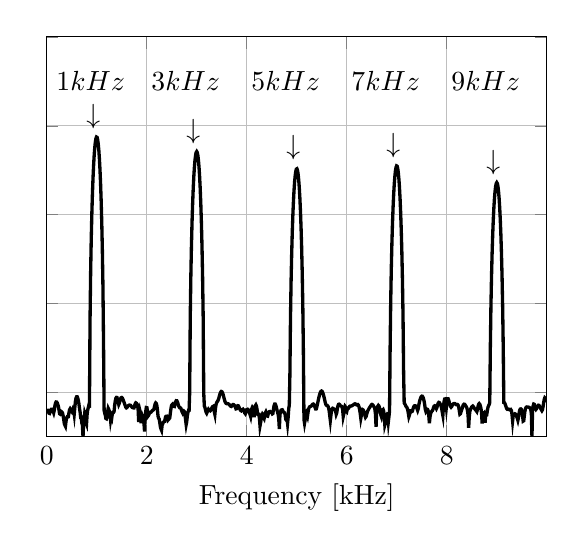
\begin{tikzpicture}

\begin{axis}[%
width=2.5in,
height=2in,
at={(1.011in,0.642in)},
scale only axis,
scaled x ticks = false,
xmin=0,
xmax=10000,
xlabel={Frequency [kHz]},
xmajorgrids,
ymin=-350,
ymax=100,
yticklabels={\empty},
xticklabels={0, 2, 4, 6, 8},
xtick = {0, 2000, 4000, 6000, 8000},
ymajorgrids,
axis background/.style={fill=white}
]
\addplot [color=black,solid,line width=1.2pt,forget plot]
  table[row sep=crcr]{%
0	-319.66977604872\\
11.7216117216117	-320.252664587285\\
23.4432234432234	-320.150235457912\\
35.1648351648352	-321.87769890753\\
46.8864468864469	-323.40415662653\\
58.6080586080586	-323.656130393623\\
70.3296703296703	-322.064437707905\\
82.0512820512821	-319.981208617154\\
93.7728937728938	-318.842227630664\\
105.494505494505	-318.824139809043\\
117.216117216117	-320.887574922404\\
128.937728937729	-321.003133041111\\
140.659340659341	-322.87596816246\\
152.380952380952	-319.992614901689\\
164.102564102564	-315.14338512313\\
175.824175824176	-312.091040412566\\
187.545787545788	-310.719044223205\\
199.267399267399	-310.809798667983\\
210.989010989011	-311.752989871661\\
222.710622710623	-313.45380396223\\
234.432234432234	-315.761867809304\\
246.153846153846	-319.502071438942\\
257.875457875458	-323.946635313474\\
269.59706959707	-324.371444723204\\
281.318681318681	-323.073351060989\\
293.040293040293	-321.551796444871\\
304.761904761905	-322.055919814239\\
316.483516483516	-322.965971780673\\
328.205128205128	-326.002185265755\\
339.92673992674	-329.965312555944\\
351.648351648352	-334.711128765065\\
363.369963369963	-336.638049322374\\
375.091575091575	-337.98571585667\\
386.813186813187	-332.646513976849\\
398.534798534799	-328.549789756313\\
410.25641025641	-327.456662133417\\
421.978021978022	-327.626158860462\\
433.699633699634	-327.386942727765\\
445.421245421245	-322.896618361246\\
457.142857142857	-319.559352515529\\
468.864468864469	-318.409730305314\\
480.586080586081	-319.522058201484\\
492.307692307692	-320.47758374283\\
504.029304029304	-321.509888136428\\
515.750915750916	-320.159719568534\\
527.472527472527	-318.379124501943\\
539.194139194139	-319.523442928177\\
550.915750915751	-324.291519604555\\
562.637362637363	-317.000247172954\\
574.358974358974	-310.257297372003\\
586.080586080586	-306.452256789241\\
597.802197802198	-304.914755096574\\
609.52380952381	-304.849950666219\\
621.245421245421	-306.178349309972\\
632.967032967033	-308.999456883321\\
644.688644688645	-312.701079748048\\
656.410256410256	-318.133369508358\\
668.131868131868	-321.871349328687\\
679.85347985348	-328.007141062136\\
691.575091575092	-327.923815494954\\
703.296703296703	-334.421366290934\\
715.018315018315	-336.919165990102\\
726.739926739927	-350.238350354447\\
738.461538461538	-334.287106214054\\
750.18315018315	-331.529493482922\\
761.904761904762	-323.393743024448\\
773.626373626374	-325.375012877451\\
785.347985347985	-333.280057572197\\
797.069597069597	-335.19416243948\\
808.791208791209	-324.722376849988\\
820.512820512821	-319.534300482415\\
832.234432234432	-317.094423031942\\
843.956043956044	-314.230543015098\\
855.677655677656	-314.557553385869\\
867.399267399267	-218.096479418237\\
879.120879120879	-165.31233950964\\
890.842490842491	-128.682095822832\\
902.564102564103	-100.530344507165\\
914.285714285714	-78.084880479123\\
926.007326007326	-59.9659632721987\\
937.728937728938	-45.374718047142\\
949.450549450549	-33.8079579109673\\
961.172161172161	-24.9340347597582\\
972.893772893773	-18.5312624507586\\
984.615384615385	-14.4548534903171\\
996.336996336996	-12.6185805249835\\
1008.05860805861	-12.9850171766986\\
1019.78021978022	-15.5615638599584\\
1031.50183150183	-20.4012212145476\\
1043.22344322344	-27.6083083479584\\
1054.94505494505	-37.3506537674849\\
1066.66666666667	-49.8819120327287\\
1078.38827838828	-65.5819960417282\\
1090.10989010989	-85.0340135297919\\
1101.8315018315	-109.185220100279\\
1113.55311355311	-139.739280721206\\
1125.27472527473	-180.395851142773\\
1136.99633699634	-243.857203771645\\
1148.71794871795	-320.064214921221\\
1160.43956043956	-323.366413363497\\
1172.16117216117	-325.396412628388\\
1183.88278388278	-329.265224803788\\
1195.6043956044	-329.60094243683\\
1207.32600732601	-326.921780096168\\
1219.04761904762	-321.464324984819\\
1230.76923076923	-317.826268547569\\
1242.49084249084	-319.221077345555\\
1254.21245421245	-321.375095535668\\
1265.93406593407	-324.721808786549\\
1277.65567765568	-331.172690405964\\
1289.37728937729	-327.190232156617\\
1301.0989010989	-328.859943718811\\
1312.82051282051	-323.934795224629\\
1324.54212454212	-322.364415478264\\
1336.26373626374	-322.478330039218\\
1347.98534798535	-321.489536953464\\
1359.70695970696	-314.390389588376\\
1371.42857142857	-309.60862386725\\
1383.15018315018	-306.521750201537\\
1394.87179487179	-305.565117533603\\
1406.59340659341	-305.702100348221\\
1418.31501831502	-307.818779142851\\
1430.03663003663	-310.811026454631\\
1441.75824175824	-313.559439282394\\
1453.47985347985	-312.058365319402\\
1465.20146520147	-309.48643321096\\
1476.92307692308	-307.140766755864\\
1488.64468864469	-305.927929790195\\
1500.3663003663	-305.68081936221\\
1512.08791208791	-306.253463667057\\
1523.80952380952	-307.512548043642\\
1535.53113553114	-309.240333775713\\
1547.25274725275	-311.110810007732\\
1558.97435897436	-313.026613238936\\
1570.69597069597	-314.684246329279\\
1582.41758241758	-316.562263550235\\
1594.13919413919	-317.34925468497\\
1605.86080586081	-316.972914787236\\
1617.58241758242	-315.837162513633\\
1629.30402930403	-315.010289548155\\
1641.02564102564	-314.61272550257\\
1652.74725274725	-314.191796909467\\
1664.46886446886	-314.28452593732\\
1676.19047619048	-314.44068736787\\
1687.91208791209	-315.163984330929\\
1699.6336996337	-316.074197397418\\
1711.35531135531	-316.88489131864\\
1723.07692307692	-317.041914340833\\
1734.79853479853	-317.437076599362\\
1746.52014652015	-317.408595347971\\
1758.24175824176	-314.977242717819\\
1769.96336996337	-312.798692171014\\
1781.68498168498	-311.696012513731\\
1793.40659340659	-312.054973498482\\
1805.12820512821	-312.757629044374\\
1816.84981684982	-314.671182783884\\
1828.57142857143	-318.737367209963\\
1840.29304029304	-333.298637671399\\
1852.01465201465	-324.040270018849\\
1863.73626373626	-320.218772715714\\
1875.45787545788	-322.961277404956\\
1887.17948717949	-334.539879130504\\
1898.9010989011	-329.519558463716\\
1910.62271062271	-327.086665233421\\
1922.34432234432	-329.320914289439\\
1934.06593406593	-333.764791120093\\
1945.78754578755	-334.533536266036\\
1957.50915750916	-344.075961360429\\
1969.23076923077	-325.931436360931\\
1980.95238095238	-321.560515034589\\
1992.67399267399	-316.983261750671\\
2004.3956043956	-317.110381405833\\
2016.11721611722	-321.132995230379\\
2027.83882783883	-326.523077686188\\
2039.56043956044	-325.653710578744\\
2051.28205128205	-323.928172040114\\
2063.00366300366	-322.747947786259\\
2074.72527472527	-322.260325203462\\
2086.44688644689	-322.179587255979\\
2098.1684981685	-321.447015430713\\
2109.89010989011	-320.679145880763\\
2121.61172161172	-319.996850102969\\
2133.33333333333	-319.748987981692\\
2145.05494505495	-318.811608861215\\
2156.77655677656	-315.677040406118\\
2168.49816849817	-312.982927012805\\
2180.21978021978	-311.768582374902\\
2191.94139194139	-312.361349170269\\
2203.663003663	-314.717024595332\\
2215.38461538462	-319.600639416848\\
2227.10622710623	-326.758844918533\\
2238.82783882784	-328.904449591274\\
2250.54945054945	-329.992103956622\\
2262.27106227106	-333.893348006191\\
2273.99267399267	-338.599091466457\\
2285.71428571429	-340.965352163138\\
2297.4358974359	-342.523569304107\\
2309.15750915751	-336.765445451662\\
2320.87912087912	-335.565258332623\\
2332.60073260073	-333.4569631189\\
2344.32234432234	-332.951254029186\\
2356.04395604396	-332.674528864243\\
2367.76556776557	-329.994984991045\\
2379.48717948718	-327.258409386749\\
2391.20879120879	-326.695675890422\\
2402.9304029304	-326.676287404655\\
2414.65201465201	-328.264297481345\\
2426.37362637363	-331.133002458237\\
2438.09523809524	-330.432637449573\\
2449.81684981685	-329.535023454296\\
2461.53846153846	-328.791646558295\\
2473.26007326007	-323.424920352782\\
2484.98168498168	-318.460018564717\\
2496.7032967033	-314.691219196617\\
2508.42490842491	-313.711392542011\\
2520.14652014652	-313.067394364558\\
2531.86813186813	-314.016279106977\\
2543.58974358974	-315.634969727647\\
2555.31135531136	-315.816934484372\\
2567.03296703297	-313.100967181084\\
2578.75457875458	-310.464193572589\\
2590.47619047619	-309.262262083557\\
2602.1978021978	-309.311255100885\\
2613.91941391941	-310.569261034711\\
2625.64102564103	-312.500205228524\\
2637.36263736264	-314.761756514628\\
2649.08424908425	-316.412573490754\\
2660.80586080586	-317.291190858618\\
2672.52747252747	-317.313991378883\\
2684.24908424908	-317.942974517788\\
2695.9706959707	-319.7342089385\\
2707.69230769231	-321.898558877662\\
2719.41391941392	-323.134909705626\\
2731.13553113553	-321.588957105158\\
2742.85714285714	-320.885605445503\\
2754.57875457875	-321.580662784063\\
2766.30036630037	-324.821452300477\\
2778.02197802198	-330.892094927682\\
2789.74358974359	-336.098023413537\\
2801.4652014652	-332.703176113955\\
2813.18681318681	-326.372946209155\\
2824.90842490842	-322.497222683491\\
2836.63003663004	-320.220801606029\\
2848.35164835165	-320.15667236125\\
2860.07326007326	-300.30570529002\\
2871.79487179487	-214.177492827452\\
2883.51648351648	-168.385261564454\\
2895.2380952381	-135.050186499224\\
2906.95970695971	-109.011900053879\\
2918.68131868132	-88.1243250034129\\
2930.40293040293	-71.2518156639137\\
2942.12454212454	-57.7144375482064\\
2953.84615384615	-47.0758016147511\\
2965.56776556777	-39.0459280367578\\
2977.28937728938	-33.4315280345184\\
2989.01098901099	-30.1088642243201\\
3000.7326007326	-29.0087381705451\\
3012.45421245421	-30.1088642243202\\
3024.17582417582	-33.4315280345187\\
3035.89743589744	-39.0459280367583\\
3047.61904761905	-47.0758016147517\\
3059.34065934066	-57.7144375482071\\
3071.06227106227	-71.2518156639152\\
3082.78388278388	-88.124325003423\\
3094.50549450549	-109.011900053981\\
3106.22710622711	-135.050186500745\\
3117.94871794872	-168.385261645028\\
3129.67032967033	-214.177514890276\\
3141.39194139194	-300.84560200681\\
3153.11355311355	-315.2569703318\\
3164.83516483516	-316.84238110397\\
3176.55677655678	-319.656198303406\\
3188.27838827839	-322.267206549707\\
3200	-323.394796361885\\
3211.72161172161	-321.831716535344\\
3223.44322344322	-320.071509664792\\
3235.16483516484	-318.862404385705\\
3246.88644688645	-319.690646580034\\
3258.60805860806	-320.415471931005\\
3270.32967032967	-320.690946536644\\
3282.05128205128	-319.710368339791\\
3293.77289377289	-318.595434038106\\
3305.49450549451	-317.036983471108\\
3317.21611721612	-316.038331017621\\
3328.93772893773	-315.662275736532\\
3340.65934065934	-317.356396019158\\
3352.38095238095	-321.760930073742\\
3364.10256410256	-324.637108569141\\
3375.82417582418	-317.710322451106\\
3387.54578754579	-313.594250633537\\
3399.2673992674	-311.479079412246\\
3410.98901098901	-310.354822336986\\
3422.71062271062	-309.501559350269\\
3434.43223443223	-307.978785454896\\
3446.15384615385	-305.738913277755\\
3457.87545787546	-303.219123772711\\
3469.59706959707	-301.020945261217\\
3481.31868131868	-299.558883503574\\
3493.04029304029	-298.894048192919\\
3504.7619047619	-299.188153921955\\
3516.48351648352	-300.3078497822\\
3528.20512820513	-302.212617063443\\
3539.92673992674	-304.639790056806\\
3551.64835164835	-307.338226654577\\
3563.36996336996	-309.670891902987\\
3575.09157509158	-311.346258045309\\
3586.81318681319	-312.237779545341\\
3598.5347985348	-312.56161470283\\
3610.25641025641	-312.55329095589\\
3621.97802197802	-312.582369772614\\
3633.69963369963	-312.851642932638\\
3645.42124542125	-313.337522432521\\
3657.14285714286	-313.980853222016\\
3668.86446886447	-314.970961319011\\
3680.58608058608	-315.519669753624\\
3692.30769230769	-315.771476529355\\
3704.0293040293	-315.073491592498\\
3715.75091575092	-314.189266101827\\
3727.47252747253	-313.593883592026\\
3739.19413919414	-313.738638685608\\
3750.91575091575	-314.308512255133\\
3762.63736263736	-315.339022840772\\
3774.35897435897	-316.603604206891\\
3786.08058608059	-318.480880716564\\
3797.8021978022	-318.292200819127\\
3809.52380952381	-316.112351446803\\
3821.24542124542	-314.897423670021\\
3832.96703296703	-315.017858900632\\
3844.68864468864	-316.135152915023\\
3856.41025641026	-317.820937023667\\
3868.13186813187	-319.413847765108\\
3879.85347985348	-320.333708738422\\
3891.57509157509	-320.722670234731\\
3903.2967032967	-319.992076799159\\
3915.01831501832	-319.338489682422\\
3926.73992673993	-318.858608272676\\
3938.46153846154	-319.680816828147\\
3950.18315018315	-320.978850851144\\
3961.90476190476	-323.188232090719\\
3973.62637362637	-324.007985133895\\
3985.34798534799	-322.570195704753\\
3997.0695970696	-319.514596742841\\
4008.79120879121	-319.283053569699\\
4020.51282051282	-318.929362581139\\
4032.23443223443	-319.488742096079\\
4043.95604395604	-320.965633129066\\
4055.67765567766	-322.481527107505\\
4067.39926739927	-324.813720853809\\
4079.12087912088	-327.030843198677\\
4090.84249084249	-322.285902452843\\
4102.5641025641	-318.186243444301\\
4114.28571428571	-316.603502399595\\
4126.00732600733	-317.481479156322\\
4137.72893772894	-321.968090951304\\
4149.45054945055	-327.957840447245\\
4161.17216117216	-318.976727193473\\
4172.89377289377	-315.096300971734\\
4184.61538461538	-314.032500143688\\
4196.336996337	-315.483699263343\\
4208.05860805861	-319.265132234658\\
4219.78021978022	-324.55539249217\\
4231.50183150183	-324.788115491149\\
4243.22344322344	-324.700621521764\\
4254.94505494505	-328.989312876653\\
4266.66666666667	-337.569307608176\\
4278.38827838828	-333.952487175123\\
4290.10989010989	-329.959991603221\\
4301.8315018315	-325.799592908156\\
4313.55311355311	-324.369338201738\\
4325.27472527472	-325.364218654711\\
4336.99633699634	-328.177317631504\\
4348.71794871795	-329.373251997288\\
4360.43956043956	-325.946288654945\\
4372.16117216117	-323.093752552372\\
4383.88278388278	-321.779392892024\\
4395.6043956044	-323.48874347434\\
4407.32600732601	-326.468625864879\\
4419.04761904762	-326.651753870262\\
4430.76923076923	-324.105142382957\\
4442.49084249084	-322.360324994449\\
4454.21245421245	-321.523240426057\\
4465.93406593407	-321.416141577155\\
4477.65567765568	-322.01923713689\\
4489.37728937729	-322.277623497054\\
4501.0989010989	-322.837324311223\\
4512.82051282051	-324.131882907695\\
4524.54212454212	-323.707472016558\\
4536.26373626374	-318.734144772884\\
4547.98534798535	-314.843075442963\\
4559.70695970696	-313.072167637317\\
4571.42857142857	-313.083110435843\\
4583.15018315018	-314.523708294673\\
4594.87179487179	-316.843132095304\\
4606.59340659341	-319.946727607398\\
4618.31501831502	-322.580797757278\\
4630.03663003663	-324.643297800685\\
4641.75824175824	-330.090746214774\\
4653.47985347985	-341.115506894516\\
4665.20146520146	-325.198207363607\\
4676.92307692308	-321.391338010681\\
4688.64468864469	-319.939534104301\\
4700.3663003663	-319.595169091842\\
4712.08791208791	-319.469942141125\\
4723.80952380952	-320.605907533617\\
4735.53113553114	-321.863281040901\\
4747.25274725275	-322.505865049125\\
4758.97435897436	-322.899195500862\\
4770.69597069597	-325.654732674365\\
4782.41758241758	-330.341163475003\\
4794.13919413919	-331.246642250653\\
4805.86080586081	-329.204106508267\\
4817.58241758242	-334.885243879829\\
4829.30402930403	-328.101152331398\\
4841.02564102564	-318.294888808809\\
4852.74725274725	-314.129895112624\\
4864.46886446886	-279.651117196258\\
4876.19047619048	-216.132332330872\\
4887.91208791209	-175.475716839038\\
4899.6336996337	-144.921655735681\\
4911.35531135531	-120.770449149269\\
4923.07692307692	-101.318431660301\\
4934.79853479854	-85.6183476512476\\
4946.52014652015	-73.0870893860055\\
4958.24175824176	-63.3447439664808\\
4969.96336996337	-56.1376568330706\\
4981.68498168498	-51.2979994784815\\
4993.40659340659	-48.7214527952216\\
5005.12820512821	-48.3550161435066\\
5016.84981684982	-50.1912891088403\\
5028.57142857143	-54.2676980692819\\
5040.29304029304	-60.6704703782819\\
5052.01465201465	-69.5443935294921\\
5063.73626373626	-81.1111536656695\\
5075.45787545788	-95.7023988907233\\
5087.17948717949	-113.821316097484\\
5098.9010989011	-136.266780122429\\
5110.62271062271	-164.418531362237\\
5122.34432234432	-201.048770357836\\
5134.06593406593	-253.83120041389\\
5145.78754578755	-330.239456002953\\
5157.50915750916	-334.680801990704\\
5169.23076923077	-330.978335548456\\
5180.95238095238	-324.592108259334\\
5192.67399267399	-322.988357718612\\
5204.3956043956	-324.676605742458\\
5216.11721611722	-326.675404290512\\
5227.83882783883	-322.058554497306\\
5239.56043956044	-318.408755963627\\
5251.28205128205	-316.800667047183\\
5263.00366300366	-316.012155133395\\
5274.72527472528	-315.808538693121\\
5286.44688644689	-315.519241470069\\
5298.1684981685	-314.766546053413\\
5309.89010989011	-313.915693680535\\
5321.61172161172	-313.170309935136\\
5333.33333333333	-313.002506027263\\
5345.05494505495	-313.778996673083\\
5356.77655677656	-315.052384147386\\
5368.49816849817	-317.119258702662\\
5380.21978021978	-318.60297759862\\
5391.94139194139	-318.517609885014\\
5403.663003663	-316.146428602339\\
5415.38461538462	-313.22805094124\\
5427.10622710623	-310.060397661986\\
5438.82783882784	-307.004516563346\\
5450.54945054945	-304.11566250975\\
5462.27106227106	-301.720722823213\\
5473.99267399267	-299.876292417269\\
5485.71428571429	-298.717877556861\\
5497.4358974359	-298.340591948456\\
5509.15750915751	-298.817309497537\\
5520.87912087912	-300.084771537962\\
5532.60073260073	-302.0378396415\\
5544.32234432234	-304.538277896337\\
5556.04395604396	-307.406392708756\\
5567.76556776557	-310.390764521531\\
5579.48717948718	-312.981246586604\\
5591.20879120879	-314.295442763613\\
5602.9304029304	-314.695913010283\\
5614.65201465201	-314.755035766114\\
5626.37362637363	-315.582819583783\\
5638.09523809524	-317.334834104706\\
5649.81684981685	-320.766298110227\\
5661.53846153846	-326.125090381781\\
5673.26007326007	-331.431983615578\\
5684.98168498169	-325.508706127021\\
5696.7032967033	-321.15493650177\\
5708.42490842491	-318.814872500501\\
5720.14652014652	-317.817991285284\\
5731.86813186813	-318.089237603718\\
5743.58974358974	-318.611263623369\\
5755.31135531136	-318.932354317994\\
5767.03296703297	-319.606180603829\\
5778.75457875458	-321.168015391352\\
5790.47619047619	-324.529320635772\\
5802.1978021978	-322.807418670069\\
5813.91941391941	-317.983100218686\\
5825.64102564103	-314.980861521282\\
5837.36263736264	-313.408700551849\\
5849.08424908425	-313.197201859578\\
5860.80586080586	-313.697729031082\\
5872.52747252747	-314.609828464371\\
5884.24908424908	-315.273710204582\\
5895.9706959707	-315.575090179884\\
5907.69230769231	-316.431533776942\\
5919.41391941392	-319.426403749631\\
5931.13553113553	-327.076704692552\\
5942.85714285714	-324.120179770849\\
5954.57875457875	-317.664559412797\\
5966.30036630037	-315.562772389357\\
5978.02197802198	-316.481875593137\\
5989.74358974359	-320.74085073736\\
6001.4652014652	-321.56480888906\\
6013.18681318681	-318.837510142599\\
6024.90842490843	-318.106231260851\\
6036.63003663004	-317.807698890747\\
6048.35164835165	-316.558092075019\\
6060.07326007326	-315.557699772867\\
6071.79487179487	-315.235903266329\\
6083.51648351648	-315.34274333107\\
6095.2380952381	-315.20030664534\\
6106.95970695971	-314.830629275607\\
6118.68131868132	-314.427815160164\\
6130.40293040293	-314.058289013738\\
6142.12454212454	-313.517054051609\\
6153.84615384615	-313.025791554879\\
6165.56776556777	-312.730990453284\\
6177.28937728938	-312.947591502956\\
6189.01098901099	-313.543344432103\\
6200.7326007326	-314.08198534147\\
6212.45421245421	-313.975108910851\\
6224.17582417582	-313.669511020471\\
6235.89743589744	-314.37833689353\\
6247.61904761905	-316.358275023731\\
6259.34065934066	-319.674879096136\\
6271.06227106227	-323.684029643681\\
6282.78388278388	-329.039415469563\\
6294.50549450549	-325.5421152618\\
6306.22710622711	-320.930017930124\\
6317.94871794872	-319.278262636475\\
6329.67032967033	-319.693181877834\\
6341.39194139194	-320.924615001357\\
6353.11355311355	-323.079359745366\\
6364.83516483516	-325.918015706887\\
6376.55677655678	-328.033773854441\\
6388.27838827839	-327.140117854091\\
6400	-324.692133834817\\
6411.72161172161	-322.137346233329\\
6423.44322344322	-320.516820802526\\
6435.16483516484	-319.337054507976\\
6446.88644688645	-318.025709346077\\
6458.60805860806	-316.979112033717\\
6470.32967032967	-315.931251445007\\
6482.05128205128	-315.062076374335\\
6493.77289377289	-313.906631470696\\
6505.49450549451	-313.466921344982\\
6517.21611721612	-313.769319638734\\
6528.93772893773	-314.517640921084\\
6540.65934065934	-315.724484282667\\
6552.38095238095	-316.588068571762\\
6564.10256410256	-318.855919571499\\
6575.82417582418	-324.361412166511\\
6587.54578754579	-338.649091166889\\
6599.2673992674	-322.760921159812\\
6610.98901098901	-317.753906925668\\
6622.71062271062	-315.516352483433\\
6634.43223443223	-314.526286365145\\
6646.15384615385	-315.259688478357\\
6657.87545787546	-317.394762548319\\
6669.59706959707	-320.732967861906\\
6681.31868131868	-324.825744034868\\
6693.04029304029	-326.820759935945\\
6704.7619047619	-322.872146846357\\
6716.48351648352	-319.74872153185\\
6728.20512820513	-319.170904101219\\
6739.92673992674	-321.086066713475\\
6751.64835164835	-326.112025334888\\
6763.36996336996	-336.624474419805\\
6775.09157509157	-334.230732856827\\
6786.81318681319	-328.753062556712\\
6798.5347985348	-326.073886014491\\
6810.25641025641	-324.70176008207\\
6821.97802197802	-325.405825297174\\
6833.69963369963	-332.73783740919\\
6845.42124542125	-327.048455871861\\
6857.14285714286	-320.875104728307\\
6868.86446886447	-250.574647660477\\
6880.58608058608	-197.792799172064\\
6892.30769230769	-161.162560617437\\
6904.0293040293	-133.010809320255\\
6915.75091575092	-110.565345290186\\
6927.47252747253	-92.4464280830486\\
6939.19413919414	-77.8551828579892\\
6950.91575091575	-66.2884227218201\\
6962.63736263736	-57.4144995706133\\
6974.35897435897	-51.0117272616143\\
6986.08058608059	-46.9353183011729\\
6997.8021978022	-45.0990453358394\\
7009.52380952381	-45.4654819875546\\
7021.24542124542	-48.0420286708145\\
7032.96703296703	-52.8816860254038\\
7044.68864468864	-60.0887731588147\\
7056.41025641026	-69.8311185783417\\
7068.13186813187	-82.3623768435883\\
7079.85347985348	-98.0624608526129\\
7091.57509157509	-117.514478341006\\
7103.2967032967	-141.665684918764\\
7115.01831501831	-172.219745862912\\
7126.73992673993	-212.876362575016\\
7138.46153846154	-276.422779719188\\
7150.18315018315	-311.898684092958\\
7161.90476190476	-312.709742302499\\
7173.62637362637	-314.073994262169\\
7185.34798534799	-315.509132701049\\
7197.0695970696	-316.40719601034\\
7208.79120879121	-317.332582010188\\
7220.51282051282	-319.40750609588\\
7232.23443223443	-323.210664245618\\
7243.95604395604	-327.331928901919\\
7255.67765567766	-325.473483569222\\
7267.39926739927	-321.976013289618\\
7279.12087912088	-320.676201014468\\
7290.84249084249	-320.801210307641\\
7302.5641025641	-321.507756558202\\
7314.28571428571	-321.103460465869\\
7326.00732600733	-318.588086156553\\
7337.72893772894	-316.565075206643\\
7349.45054945055	-315.277346593938\\
7361.17216117216	-314.885550260067\\
7372.89377289377	-314.891837602016\\
7384.61538461538	-315.449350147104\\
7396.336996337	-316.745745681702\\
7408.05860805861	-318.419916282407\\
7419.78021978022	-320.261431969836\\
7431.50183150183	-318.268672120946\\
7443.22344322344	-314.091608173447\\
7454.94505494505	-310.765957845321\\
7466.66666666667	-308.217783141544\\
7478.38827838828	-306.239035860403\\
7490.10989010989	-304.816952750248\\
7501.8315018315	-304.15608386294\\
7513.55311355311	-304.254491064508\\
7525.27472527472	-305.211593460601\\
7536.99633699634	-307.030312830436\\
7548.71794871795	-309.879326533619\\
7560.43956043956	-313.845760685343\\
7572.16117216117	-318.841850332976\\
7583.88278388278	-321.207995748871\\
7595.6043956044	-320.013712544925\\
7607.32600732601	-318.776063684063\\
7619.04761904762	-319.085551795786\\
7630.76923076923	-320.939164664321\\
7642.49084249084	-326.254817057014\\
7654.21245421245	-334.569473846894\\
7665.93406593407	-327.931786824776\\
7677.65567765568	-324.051596359106\\
7689.37728937729	-322.288144039605\\
7701.0989010989	-321.229303753046\\
7712.82051282051	-320.657714719804\\
7724.54212454212	-319.352677742086\\
7736.26373626374	-317.11201010275\\
7747.98534798535	-315.512568863074\\
7759.70695970696	-314.929278878524\\
7771.42857142857	-315.115340679379\\
7783.15018315018	-316.822691426277\\
7794.87179487179	-318.181220637214\\
7806.59340659341	-316.776568611525\\
7818.31501831502	-313.852220867404\\
7830.03663003663	-312.002406009657\\
7841.75824175824	-311.164749597181\\
7853.47985347985	-311.393965980471\\
7865.20146520146	-312.252662903959\\
7876.92307692308	-313.70152247797\\
7888.64468864469	-315.573585771477\\
7900.3663003663	-318.092576192861\\
7912.08791208791	-322.4419386204\\
7923.80952380952	-325.885107269\\
7935.53113553114	-315.728036603532\\
7947.25274725275	-310.207096026785\\
7958.97435897436	-307.39528878069\\
7970.69597069597	-307.214798035391\\
7982.41758241758	-310.249964168014\\
7994.13919413919	-316.455301461558\\
8005.86080586081	-310.18108881179\\
8017.58241758242	-307.118104234728\\
8029.30402930403	-307.103626006243\\
8041.02564102564	-308.787848887118\\
8052.74725274725	-311.254474300167\\
8064.46886446886	-313.705378738313\\
8076.19047619048	-315.670416772103\\
8087.91208791209	-316.586732731561\\
8099.6336996337	-315.828567102877\\
8111.35531135531	-314.658811303786\\
8123.07692307692	-313.406572522504\\
8134.79853479854	-312.66962362792\\
8146.52014652015	-312.448750110159\\
8158.24175824176	-312.419482694733\\
8169.96336996337	-312.803696384012\\
8181.68498168498	-313.295545576826\\
8193.40659340659	-313.853348514964\\
8205.12820512821	-313.833478550749\\
8216.84981684982	-313.61336866691\\
8228.57142857143	-314.193969835242\\
8240.29304029304	-316.283557504146\\
8252.01465201465	-320.403424674361\\
8263.73626373626	-324.461982722269\\
8275.45787545788	-323.928707340462\\
8287.17948717949	-321.76611077263\\
8298.9010989011	-319.645859437962\\
8310.62271062271	-317.756972073173\\
8322.34432234432	-315.456535213765\\
8334.06593406593	-313.801900724168\\
8345.78754578755	-313.156054469238\\
8357.50915750916	-313.295300275638\\
8369.23076923077	-314.015963323273\\
8380.95238095238	-315.107651529325\\
8392.67399267399	-316.0289335874\\
8404.3956043956	-317.664437763639\\
8416.11721611722	-320.322192776584\\
8427.83882783883	-325.454646046237\\
8439.56043956044	-339.882811871287\\
8451.28205128205	-327.930659862074\\
8463.00366300366	-321.508748618535\\
8474.72527472528	-319.142368328328\\
8486.44688644689	-317.887625168224\\
8498.1684981685	-316.398702897209\\
8509.89010989011	-315.844272704648\\
8521.61172161172	-315.304129811956\\
8533.33333333333	-315.994408548112\\
8545.05494505494	-316.988551478669\\
8556.77655677656	-318.106390240229\\
8568.49816849817	-319.027154929891\\
8580.21978021978	-319.812320525615\\
8591.94139194139	-320.557458360575\\
8603.663003663	-321.51609417813\\
8615.38461538462	-319.208436155719\\
8627.10622710623	-315.634876225168\\
8638.82783882784	-313.282580117098\\
8650.54945054945	-312.557824637183\\
8662.27106227106	-313.287365657449\\
8673.99267399267	-315.101223185669\\
8685.71428571429	-317.918900259002\\
8697.4358974359	-322.827357182022\\
8709.15750915751	-334.905660533007\\
8720.87912087912	-329.598732480268\\
8732.60073260073	-323.918402497209\\
8744.32234432235	-323.225663253841\\
8756.04395604396	-327.882604758779\\
8767.76556776557	-334.08772192061\\
8779.48717948718	-325.816032287453\\
8791.20879120879	-324.120639882715\\
8802.9304029304	-324.463360873992\\
8814.65201465201	-320.157644074005\\
8826.37362637363	-316.607378912133\\
8838.09523809524	-314.977460763074\\
8849.81684981685	-313.598892848365\\
8861.53846153846	-311.531251182091\\
8873.26007326007	-249.039767111074\\
8884.98168498169	-203.242029131657\\
8896.7032967033	-169.906929318669\\
8908.42490842491	-143.868642611774\\
8920.14652014652	-122.981067561458\\
8931.86813186813	-106.108558222317\\
8943.58974358974	-92.5711801065715\\
8955.31135531135	-81.9325441730846\\
8967.03296703297	-73.9026705950811\\
8978.75457875458	-68.2882705928396\\
8990.47619047619	-64.9656067826414\\
9002.1978021978	-63.8654807288671\\
9013.91941391941	-64.9656067826429\\
9025.64102564103	-68.2882705928421\\
9037.36263736264	-73.9026705950824\\
9049.08424908425	-81.9325441730767\\
9060.80586080586	-92.5711801065311\\
9072.52747252747	-106.108558222202\\
9084.24908424908	-122.981067561203\\
9095.9706959707	-143.868642602562\\
9107.69230769231	-169.906928781367\\
9119.41391941392	-203.241987404462\\
9131.13553113553	-249.030296777096\\
9142.85714285714	-311.304512921604\\
9154.57875457876	-311.537328657934\\
9166.30036630037	-312.622507182141\\
9178.02197802198	-314.484101268501\\
9189.74358974359	-316.638047956377\\
9201.4652014652	-318.240365114368\\
9213.18681318681	-318.945193216639\\
9224.90842490842	-318.716534544361\\
9236.63003663004	-318.771748632388\\
9248.35164835165	-318.836599674886\\
9260.07326007326	-319.61908906793\\
9271.79487179487	-319.822294152504\\
9283.51648351648	-319.371461582341\\
9295.2380952381	-320.455571545465\\
9306.95970695971	-324.955116608097\\
9318.68131868132	-332.064216057748\\
9330.40293040293	-326.151615205209\\
9342.12454212454	-324.758080768938\\
9353.84615384615	-324.675211282058\\
9365.56776556777	-324.045321612164\\
9377.28937728938	-324.39253747893\\
9389.01098901099	-325.618923679901\\
9400.7326007326	-327.30803370137\\
9412.45421245421	-329.101453300761\\
9424.17582417582	-331.357262728207\\
9435.89743589744	-328.369864579068\\
9447.61904761905	-323.625954295584\\
9459.34065934066	-320.052944616956\\
9471.06227106227	-318.680325028373\\
9482.78388278388	-318.495481334863\\
9494.50549450549	-319.072602246417\\
9506.22710622711	-322.438351004492\\
9517.94871794872	-326.302775164653\\
9529.67032967033	-332.236401444499\\
9541.39194139194	-331.826732588463\\
9553.11355311355	-326.312560073614\\
9564.83516483517	-321.103996076185\\
9576.55677655678	-318.036729405502\\
9588.27838827839	-316.757057599893\\
9600	-316.289063164499\\
9611.72161172161	-316.324856775091\\
9623.44322344322	-316.350179630349\\
9635.16483516483	-316.563172794392\\
9646.88644688645	-316.736600642076\\
9658.60805860806	-317.140959522388\\
9670.32967032967	-317.883238263279\\
9682.05128205128	-319.49921625628\\
9693.77289377289	-323.692303015967\\
9705.49450549451	-349.984618262359\\
9717.21611721612	-320.976769185242\\
9728.93772893773	-315.17753537576\\
9740.65934065934	-313.074148193045\\
9752.38095238095	-313.376471369528\\
9764.10256410256	-315.248048467012\\
9775.82417582418	-317.460020635791\\
9787.54578754579	-318.916164496397\\
9799.2673992674	-318.079181600956\\
9810.98901098901	-316.690886394991\\
9822.71062271062	-315.207508754715\\
9834.43223443223	-314.386564565063\\
9846.15384615385	-314.548895431942\\
9857.87545787546	-315.391776864814\\
9869.59706959707	-316.68455315035\\
9881.31868131868	-318.139278296883\\
9893.04029304029	-319.449803507901\\
9904.7619047619	-320.515956568989\\
9916.48351648352	-319.388496977814\\
9928.20512820513	-315.730857337976\\
9939.92673992674	-311.242165481577\\
9951.64835164835	-307.737829406979\\
9963.36996336996	-305.870078981667\\
9975.09157509158	-306.441379041955\\
9986.81318681319	-310.96576225089\\
};
\node[right, align=left, text=black]
at (axis cs:600,10) {$\downarrow$};
\node[right, align=left, text=black]
at (axis cs:0,50) {$\text{1 kHz}$};
\node[right, align=left, text=black]
at (axis cs:2600,-6) {$\downarrow$};
\node[right, align=left, text=black]
at (axis cs:1900,50) {$\text{3 kHz}$};
\node[right, align=left, text=black]
at (axis cs:4600,-25) {$\downarrow$};
\node[right, align=left, text=black]
at (axis cs:3900,50) {$\text{5 kHz}$};
\node[right, align=left, text=black]
at (axis cs:6600,-22) {$\downarrow$};
\node[right, align=left, text=black]
at (axis cs:5900,50) {$\text{7 kHz}$};
\node[right, align=left, text=black]
at (axis cs:8600,-41) {$\downarrow$};
\node[right, align=left, text=black]
at (axis cs:7900,50) {$\text{9 kHz}$};
\end{axis}
\end{tikzpicture}%
	\caption{FFT of a 1 kHz sinusoid with clipping.}
	\label{fig:clippingDistFFT}
\end{subfigure}
\caption{The Fast Fourier Transformation(FFT) of the 1 kHz sinusoid with a peak amplitude on 1.5. }
\label{fig:audioclippingFFT}
\end{figure}

%The sampling frequency is 48 kHz and a Kaiser-window function with a $\beta$-value of 38 is applied to both signal.
The amplitude difference between the fundamental frequency on 1 kHz and the 3rd harmonic frequency is 16 dB, which is approximately a factor of 6.3 in linear scale. If the signal is clipped even more, the amplitude difference between the fundamental frequency and uneven harmonics decreases thus making it even more unpleasant. Therefore audio clipping should be avoided or minimized.












\section{Loudspeaker topology}

In order to understand where distortion could arrive from in a speaker it is necessary to understand the basic fundamentals and the topology of a loudspeaker. This section will consist of the basic topology and then glans over the topic of vibration induced in the speaker driver.

\subsubsection*{The basics}
The loudspeaker is a transducer which purpose is to convert the electrical energy into acoustical energy. This is done by sending the signal into the speaker which can consist of numerous driver. Each driver is made with a specific purpose for handling frequency. The drivers are designed to perform best within their frequency range, hence they are usually different sizes in diameter.
\begin{itemize}
\item[] For the high frequencies their is a tweeter, 1-2 inches in diameters, high frequencies is roughly 3-4 kHz and above.
\item[] In the midrange their is a midrange driver which usually is around 5-6 inches. The midrange is roughly 3-4 kHz to 300 Hz. 
\item[] The lower frequencies, which is 300 and below, is then handled by the woofer. The woofer can is usually 5-6+ inches in diameter.
\end{itemize}
The reason for different diameters in drivers is because of the wavelength the specific frequencies got. Should a woofer play frequencies at +4 kHz it would end in the driver physically not being able to move that fast. The limitations will end up in non-linear distortion in the diaphragm. Vice versa, should a tweeter reproduced low frequency sound at high \gls{SPL} it will end in distortion. The tweeter has a very low excursion range which limits it to the high frequency area.

\subsubsection*{Sensitivity}

A speaker is supplied from the manufacture with a sensitivity rating. This tells how efficient a loudspeaker is. The sensitivity rating is rated in dB and tells what \gls{SPL} the speaker outputs when supplied with 1 watt using 2.86 volt and measured at 1 meter. This is done assuming an infinite baffle and no reflection from the room. The sensitivity is defined by \autoref{eq:speaker_sensitivty}.
\begin{align}\label{eq:speaker_sensitivty}
\text{dB}_\text{sensitivity}=112\text {dB} +10 \cdot log_{10}(\text{efficiency})
\end{align}  
The 112 dB in \autoref{eq:speaker_sensitivty} is added to the sensitivity since this 1 watt compared to the $10^{-12}$ watt which is the threshold for audible sound. At 1 watt it will yield 120 dB. The reason for 8 dB difference is due to the assumption of infinite baffle in a reflection free room. When the sound is dispersed at a radius of $2\pi=r^2$, where r is 1 meter it creates a reduction in \gls{SPL} by 8 dB.

\subsubsection*{Diaphragm excursion}




\subsection{Distortion from vibration}

A common problem when designing loudspeakers is the vibrations from the enclosure. If the vibrations are strong, they will become audible and distort the overall sound. The sound radiation from the enclosure will become greater when the \gls{SPL} from the speaker increase. This problem is solved with different techniques but yield more or less the same outcome, which is stiffening of the enclosure. Some of the techniques for removing vibrations from the enclosure could be:
\begin{itemize}
\item Mechanical decoupling of the drivers from the enclosure.
\item Denser or heavier construction material with a high natural frequency, making it harder for the enclosure to start vibrating.
\item Dampening material or complex structural design inside the cabinet to disperse the sound.
\end{itemize}
\todo[inline]{Skal nok lige skaffe nogle kilder på de udtagelser}


Looking further into the speaker driver itself, it shows in \autoref{fig:SpeakerModelStress} that parts in the driver also creates unwanted vibrations. The goal of the speaker driver is to reproduce the electrical signal as an acoustical signal. This is done by using a membrane which is suspended in a very light and easy to move material. An Induction in the coil is created in a permanent magnet creating a a electro magnetic force resulting in the membrane moving. The goal will always be to loose as little as possible energy, giving the most perfect output. The driver simply needs to be as powerfull, light, stiff and efficient as possible.

\begin{figure}[H]
\centering
\begin{subfigure}[t]{0.47\textwidth}
\includegraphics[width=\linewidth]{SpeakerGOOD}
	\caption{Regular speaker driver showing suspension, membrane and the driver magnet.}
	\label{fig:regularspeaker}
\end{subfigure}
\hspace{6mm} 
\begin{subfigure}[t]{0.47\textwidth}
\includegraphics[width=\linewidth]{SpeakerBAD}
	\caption{Regular speaker driver with red markings showing stress areas}
	\label{fig:badspeaker}
\end{subfigure}
\caption{A Speaker driver, where \ref{fig:badspeaker} shows the stress points outlined with red.}
\label{fig:SpeakerModelStress}
\end{figure}

When this signal has a large amplitude, read overload, the membrane reaches physical capacity. In \autoref{fig:badspeaker} it shows that when a membrane is pushed to its maximum capacity the suspension will affect the membrane causing unwanted distortion. This will be one of the major problems if the membrane is assumed sufficiently stiff to with stand the high \gls{SPL} and not twist during playback. 

Another notice is the membrane hitting the coil connected to the magnet. This would again result in distortion since the membrane is now again hitting the absolute furthest position possible. This situation can however be resolve be moving the magnet further back. This would make the suspension determine how far the membrane can be pushed.


%that occurs at playback. The vibrations occurs because the  If the vibration. the sound radiated from the loudspeaker enclosure

%\section{Part Conclusion}
This chapter has analyzed an active speaker and its components to investigate how distortion is created throughout the active loudspeaker. The conclusion is that the following situations create distortion.
\begin{itemize}
\item Amplifier
	\begin{itemize}
	\item Clipping.
	\end{itemize}
\item Loudspeaker
	\begin{itemize}
	\item Vibrations from enclosure.
	\item Overexcursion.
	\item Membrane hitting the coil.
	\end{itemize}
\end{itemize}
Of these situations the focus moving forward will only be concerning the distortion situation from the loudspeaker because clipping in the amplifier is easy to solve, because the parameters in the amplifier is constant and the signal is easily limited to create less distortion then by hard clipping. The next chapter will therefore explain and analyze performance tests of a loudspeaker to see if any of the above loudspeaker situations can be detected. 

%\chapter{Test of DALI Zensor 5}
This section will go through a test of a loudspeaker to understand if any vibrations in the loudspeaker affect the distortion of the loudspeaker.
The loudspeaker which will be the basis for the test is the Zensor 5 (as seen on \autoref{fig:dali_zensor5}) given by DALI. A passive speaker has been choosen for the test because the amplifiers in DALI's active speakers are designed not to stress the loudspeaker to its limits and beyond, and to be able to test how the vibrations affect distortion, the loudspeaker must be tested to its limits and beyond.

\begin{figure}[H]
\centering
\includegraphics[width=0.5\textwidth]{figures/zensor5.png}
\caption{DALI zensor 5.}
\label{fig:dali_zensor5}
\end{figure}

%\todo[inline]{Reference http://www.dali-speakers.com/loudspeakers/zensor/zensor-5/}

For measuring the vibrations inside the enclosure two accelometers have been placed inside the enclosure, one on the back of bottom driver and one on the top back of the enclosure. For measuring distortion a microphone has been placed 1 m from the speaker. To limit any reflection from a room for example, the test is perfomed in the Anechoic room at \gls{AAU} see \ref{fig:test_setup_R}.  
%\todo[inline]{Reference (09.03.2016) http://doc.es.aau.dk/labs/acoustics/facilities/anechoic_room_large/} 

\begin{figure}[H]
\centering
\begin{subfigure}[t]{0.47\textwidth}
	\centering
	\includegraphics[width=1\textwidth]{figures/Test_setup_behind.jpg}
	\caption{Test setup (behind)}
	\label{fig:test_setup_behind_R}
\end{subfigure}
\hspace{6mm} 
\begin{subfigure}[t]{0.47\textwidth}
	\centering
	\includegraphics[width=1\textwidth]{figures/Test_setup_front.jpg}
	\caption{Test setup (front)}
	\label{fig:test_setup_front_R}
\end{subfigure}
\caption{Test setup.}
\label{fig:test_setup_R}
\end{figure}

The loudspeaker is set to play a sinesweep from the crossover frequency of the speaker which is 2400 Hz to 10 Hz. The sine sweep is then repeated from the lowest volume setting of an power amplifier until the loudspeaker breaks. This resulted in 20 sine sweep measurements from all three sensors which can be seen in the full test jounal in \autoref{app:journal_speaker_test}.    


\section{Analysis of the DALI Zensor AX 5 measurements}

In this section an analysis of the data extracted from the test DALI Zensor 5 AX will be presented. The purpose of this analysis is to examine if it possible to tell the current performance of the loudspeaker from the accelerometer placed on the loudspeaker. There are many different approaches in analysing the measured data, and the extent of the analysis will be analysing the frequency response of the loudspeaker vibration, harmonic distortion, and detection of the coil hitting the back plate of the driver. The structure of the following part of this section will be:

\begin{itemize}
\item Presentation of the measured data.
\item Frequency response of the measured data.
\item Harmonic distortion measured by the microphone and accelerometers.
\item Back plate hit detection.
\end{itemize}

Before analysing the measured the measured data will be presented.

All of the raw data sample and scripts used can be found on:\\
\scalebox{0.7}{
\path{CD://Maalinger/Maalinger030316 - Loudspeaker test}}\\
\scalebox{0.7}{
\path{CD://Maalinger/Maalinger030316 - Loudspeaker test/Measurements030316/MeasurementAnalysis.m}}


\section{Introduction to Measured Data}

As previously stated there are in total 20 datasets each containing four measurements, namely the vibrations from the enclosure and driver, the sound pressure from the microphone, and lastly a reference signal to synchronize all data. The amount of data is therefore large and only relevant datasets will be presented. The remaining data are available on the CD. The first dataset from the test is shown in \autoref{fig:raw1}.

\begin{figure}[H]
\centering
\begin{subfigure}[t]{0.335\textwidth}
	\includegraphics[width=1\textwidth]{figures/raw_driver1.pdf}
	\caption{Vibration from driver.}
	\label{fig:raw_driver1}
\end{subfigure}
\begin{subfigure}[t]{0.3\textwidth}
	\includegraphics[width=1\textwidth]{figures/raw_enclosure1.pdf}
	\caption{Vibration from enclosure.}
	\label{fig:raw_enclosure1}
\end{subfigure}
\begin{subfigure}[t]{0.3\textwidth}
	\includegraphics[width=1\textwidth]{figures/raw_microphone1.pdf}
	\caption{Sound pressure from microphone.}
	\label{fig:raw_microphone1}
\end{subfigure}
\caption{The measured data of (a) the vibration on the driver, (b) the vibration on the enclosure, and (c) the sound pressure from the microphone. Dataset 1.}
\label{fig:raw1}
\end{figure} 


Looking at the first dataset reveals that there are mechanical issues with the loudspeaker. In \autoref{fig:raw_driver1} there is a strong indication of a resonance frequency at 25 seconds with a peak amplitude on approximately 0.02. A similar observation can be found in \autoref{fig:raw_enclosure1} which shows the vibration measured by the accelerometer placed on the enclosure where a resonance frequency appears after 25 seconds. Another mechanical resonance frequency can be found located after 14 seconds for the enclosure. The sound pressure level measured by the microphone is in contrast fairly linear compared to the measured vibrations. Dataset 10 is shown in \autoref{fig:raw10} where the gain is increased by 10 dB.

\begin{figure}[H]
\centering
\begin{subfigure}[t]{0.335\textwidth}
	\includegraphics[width=1\textwidth]{figures/raw_driver10.pdf}
	\caption{Vibration from driver.}
	\label{fig:raw_driver10}
\end{subfigure}
\begin{subfigure}[t]{0.3\textwidth}
	\includegraphics[width=1\textwidth]{figures/raw_enclosure10.pdf}
	\caption{Vibration from enclosure.}
	\label{fig:raw_enclosure10}
\end{subfigure}
\begin{subfigure}[t]{0.3\textwidth}
	\includegraphics[width=1\textwidth]{figures/raw_microphone10.pdf}
	\caption{Sound pressure from microphone.}
	\label{fig:raw_microphone10}
\end{subfigure}
\caption{The measured data of (a) the vibration on the driver, (b) the vibration on the enclosure, and (c) the sound pressure from the microphone. Dataset 10.}
\label{fig:raw10}
\end{figure} 

The measurements from dataset 10 is very similar to the measurements seen in dataset 1. Since no particular change is happening between dataset 1 to 10 it is assumed that the performance of the loudspeaker remains good. A further analysis of the performance speaker will be done in the analysis of the harmonic distortion section to examine the amount of harmonic distortion present. Dataset 14 is shown in \autoref{fig:raw14}. 

\begin{figure}[H]
\centering
\begin{subfigure}[t]{0.335\textwidth}
	\includegraphics[width=1\textwidth]{figures/raw_driver14.pdf}
	\caption{Vibration from driver.}
	\label{fig:raw_driver14}
\end{subfigure}
\begin{subfigure}[t]{0.3\textwidth}
	\includegraphics[width=1\textwidth]{figures/raw_enclosure14.pdf}
	\caption{Vibration from enclosure.}
	\label{fig:raw_enclosure14}
\end{subfigure}
\begin{subfigure}[t]{0.3\textwidth}
	\includegraphics[width=1\textwidth]{figures/raw_microphone14.pdf}
	\caption{Sound pressure from microphone.}
	\label{fig:raw_microphone14}
\end{subfigure}
\caption{The measured data of (a) the vibration on the driver, (b) the vibration on the enclosure, and (c) the sound pressure from the microphone. Dataset 14.}
\label{fig:raw14}
\end{figure} 

While most of the measurements show the exact same characteristics as previous datasets, a slight change occurs in the end of the vibration measured on the driver in \autoref{fig:raw_driver14} and the sound pressure level in \autoref{fig:raw_microphone14}. After approximately 29 seconds a peak is observed in \autoref{fig:raw_driver14} which could indicate that the coil at that point hit the back plate of the driver. A further examination will be made in a later section. The measurements from the microphone, also show that a peak occurs at the same point, which most likely will cause the amount of harmonic distortion to increase. Dataset 19, which is the last dataset before the loudspeaker break down, is shown in \autoref{fig:raw19}.

\begin{figure}[H]
\centering
\begin{subfigure}[t]{0.335\textwidth}
	\includegraphics[width=1\textwidth]{figures/raw_driver19.pdf}
	\caption{Vibration from driver.}
	\label{fig:raw_driver19}
\end{subfigure}
\begin{subfigure}[t]{0.3\textwidth}
	\includegraphics[width=1\textwidth]{figures/raw_enclosure19.pdf}
	\caption{Vibration from enclosure.}
	\label{fig:raw_enclosure19}
\end{subfigure}
\begin{subfigure}[t]{0.3\textwidth}
	\includegraphics[width=1\textwidth]{figures/raw_microphone19.pdf}
	\caption{Sound pressure from microphone.}
	\label{fig:raw_microphone19}
\end{subfigure}
\caption{The measured data of (a) the vibration on the driver, (b) the vibration on the enclosure, and (c) the sound pressure from the microphone. Dataset 19.}
\label{fig:raw19}
\end{figure} 

Dataset 19 has the same characteristics as dataset 14, though with a more noticeable peak at 29 seconds for both the measurements from the driver and the microphone. In the last dataset shown in \autoref{fig:raw20}, the loudspeaker breaks down.


\begin{figure}[H]
\centering
\begin{subfigure}[t]{0.335\textwidth}
	\includegraphics[width=1\textwidth]{figures/raw_driver20.pdf}
	\caption{Vibration from driver.}
	\label{fig:raw_driver20}
\end{subfigure}
\begin{subfigure}[t]{0.3\textwidth}
	\includegraphics[width=1\textwidth]{figures/raw_enclosure20.pdf}
	\caption{Vibration from enclosure.}
	\label{fig:raw_enclosure20}
\end{subfigure}
\begin{subfigure}[t]{0.3\textwidth}
	\includegraphics[width=1\textwidth]{figures/raw_microphone20.pdf}
	\caption{Sound pressure from microphone.}
	\label{fig:raw_microphone20}
\end{subfigure}
\caption{The measured data of (a) the vibration on the driver, (b) the vibration on the enclosure, and (c) the sound pressure from the microphone. Dataset 20.}
\label{fig:raw20}
\end{figure} 

As seen in \autoref{fig:raw_driver20} the loudspeaker unit breaks down at the mechanical resonance frequency for the driver. The reason to why vibrations on the enclosure and sound pressure are still presentthe  after 25 seconds is because the other loudspeaker unit did not entirely break down. Since the loudspeaker unit broke down at the mechanical driver resonance frequency, it would be relevant to examine if there is any correlation as such.




% Formål

% Råt Data

% Frekvensrespons
% - Konklusion: Ikke muligt at detektere tegn på at højtaleren har nået grænsen
% - Accelerometeret kan bruges til at estimere lydtrykket

% Harmonisk forvrængning
% - Der er tydelige tegn på øget harmonisk forvrængning, når lydstyrken øges.
% - Det er dog ikke muligt at måle harmonisk forvrængning, når der er tale om musik og derfor er det ikke muligt at udvinde information om harmonisk forvrængning

% Slag detektering
% - Undersøger et givet punkt i målingerne, der ligner slag mod driveren.
% - Spektralanalyser i området viser at der sker en betydelig energinieauet i lave frekvensen.
% - Da amplitude forøgelsen ikke er forbeholdt harmoniske frekvenser, må det antages at udslagene har er i impulser der 


% Conclusion: 
% - The vibration do not affect the distortion
% - The vibration can however be used as a tool to determine the sound pressure level since there is a strong correlation between the amount of vibration and sound pressure.
% - The analysis of the hits suggest that it is possible to detect these hits by measurering very low frequenct frequencies and determine the energy increase

% Further investigation
% - Investigate the impulse response of the loudspeaker
% - Investigate if there is a if the break of the loudspeaker unit was due to the amount of vibration at the resonance frequency.








%\subsection{Frequency response of measured data}

In this section the frequency response of the measured data will be analysed to examine if there is any correlation between the frequency responses and the performance of the loudspeaker.

%\subsection{Harmonic distortion}

\textit{This section is not written yet.}

%\section{Back Plate Hit Detection}

\textit{This section is not written yet.}

\section{Problem statement} \label{sec:problem_statement}
The analysis has focused on distortion and non-linearities in an active loudspeakers different blocks. It can be concluded that most of the non-linearities are created at high sound pressure levels, which could be in the following situations:
\begin{itemize}
\item Clipping from either hard peak-limiting or amplifier.
\item Overexcursion of the diapraghm (physical clipping). 
\item Coil hitting the back plate. 
\end{itemize}

From the situations it is seen that the most critical situation would be if the coil hits the back plate because it could result in damaging or destroying the speaker. Therefore a system should be designed first and foremost to protect the speaker from being damaged. Secondly it should be designed to reduce the amount of distortion in minimum the woofer frequency range (below 200 Hz), thus avoiding peak limitation as protection. The system must be real-time as the system will be used in context with audio streaming\todo{Formulated correctly?}. With this the following problem statement is formulated:

\begin{center}
\label{ProblemStatement}
\textit{How can a real-time signal processing system in an active loudspeaker prevent the coil from hitting the back plate of the woofer and reduce distortion compared to peak limitation?}
\end{center}

Besides the problem stated above, DALI desires to have incorporated an equalizer\footnote{\scalebox{0.7}{\path{CD://MAIL/DALIRequirements.pdf}} }. % for the commercial user so it will be able to function more optimal in different room sizes. Further more it should be fully customizable for ongoing adjustments during the development period. The DALI requirements are derived via e-mail correspondence located at: \scalebox{0.7}{\path{CD://MAIL/DALIRequirements.pdf}}  



%The concept for a solution is seen on \autoref{fig:Concept}. It shows a feedback system which filters or limits a signal based on the output of sensor located in the speaker. Besides the feedback system which should protect the speaker, a user should be able to use an equalizer to change the settings of the frequency response.  
%\begin{figure}[H]
%\centering
%\tikzsetnextfilename{Concept}
%\scalebox{0.8}{
%\begin{tikzpicture}
%% Kasser %%
\node [block, fill=black!80,text=white] (AudioSource) at (0,0) {Audio Source};

%% DSP %%
%\node [block, fill=blue!15] (Equalizer1) at ($(AudioSource)+(3.5,0)$) {Equalizer};
\node [block, fill=blue!15] (SpectralAnalysis) at ($(AudioSource)+(3.5,0)$) {Signal analysis};
\node [block, fill=blue!15] (Equalizer) at ($(SpectralAnalysis)+(4.5,0)$) {Signal processing};


%% External %%
%\node [block, fill=blue!15] (UserInterface) at ($(Equalizer1)+(-3.5,2)$) {User interface};
%\node [block, fill=blue!15] (UserInterfaceDev) at ($(Equalizer1)+(3.5,2)$) {Developer interface};

%% Speaker Enclosure %%
\node [block, fill=black!80,text=white] (Amplifier) at ($(SpectralAnalysis)+(4.5,-3)$) {Amplifier};
\node [block, fill=black!80,text=white] (Driver) at ($(Amplifier)+(-3.5,0)$) {Driver};

%\node (User) at ($(-2.5,0)+(UserInterface)$) {\textbf{User}};
%\node (Developer) at ($(3.6,0)+(UserInterfaceDev)$) {\textbf{Developer}};
%\draw[->] (User) -- (UserInterface);
%\draw[->] (Developer) -- (UserInterfaceDev);

% Store Blokke %%
\begin{pgfonlayer}{background}
\draw[thick, fill=black!10] ($(-1.75,1.2)+(SpectralAnalysis)$) -- ($(2.5,1.2)+(Equalizer)$) -- ($(2.5,-1.5)+(Equalizer)$) -- ($(-1.75,-1.5)+(SpectralAnalysis)$) -- ($(-1.75,1.2)+(SpectralAnalysis)$);
\node (DSPtag) at ($(1,-1.1)+(SpectralAnalysis)$) {\textbf{Digital Processing System}};

\draw[thick, fill=black!10] ($(-2.5,1)+(Driver)$) -- ($(2.5,1)+(Amplifier)$) -- ($(2.5,-1.5)+(Amplifier)$) -- ($(-2.5,-1.5)+(Driver)$) -- ($(-2.5,1)+(Driver)$);
\node (DSPtag) at ($(2,-1.1)+(Driver)$) {\textbf{Speaker Enclosure}};
\end{pgfonlayer}

%% Forbindelse %%
\draw[->] (AudioSource) -- (SpectralAnalysis);
%\draw[->] (Equalizer1) -- (SpectralAnalysis);
\draw[->] (SpectralAnalysis) -- (Equalizer);
\draw[->] (Equalizer) -- (Amplifier);
\draw[->] (Amplifier) -- (Driver);

%\draw[->] (UserInterface) -| ($(Equalizer1)+(-.25,.6)$);
%\draw[->] (UserInterfaceDev) -| ($(Equalizer1)+(.25,.6)$);

%\draw[->] ($(SensorDriver)+(-1.375,-0.3)$) -- ($(SpectralAnalysis)+(1.375,-0.3)$);

%\draw[->] (SpectralAnalysis) -- (Decisionblock);
%\draw[->] (Decisionblock) |- (Equalizer);
\end{tikzpicture}}
%\caption{Block diagram of the concept.}
%\label{fig:Concept}
%\end{figure}
%\todo[inline]{Fiks billede}
%The concept consist of a filtering or limitation block, which will be analyzed to understand which solution is best for the problem stated, a sensor which will be analyzed to determine which sensor should be used and where it should be placed, a signal analysis block and decision block which will not be analysed furhter in this chapter, a user interface which will be analyzed to determine how the user interface should be designed and lastly the processor block which will be analyzed to detemine which type of processor that should be used. 

